\part{Ordinary Differential Equations}

This part of the text presents a course suitable for the advanced undergraduate
or beginner graduate student.  Some of the chapters have been fully fleshed
out; others are still preliminary.

I have not read it myself, but I have heard
good things about \cite{boyce:2002}.  It would be suitable for a first course.
For the more advanced student, I recommend \cite{bender:1978}, an
excellent text on the approximate solution of ordinary differential equations.
I have found \cite{zwillinger:1992} to be a very useful reference.  
For the geometric theory of ordinary differential equations and dynamical 
systems see \cite{arnold:1973} and \cite{hirsch:1974}.

\flushbottom




%%=============================================================================
%%=============================================================================
\chapter{Introduction}
\label{chapter_ode_introduction}




%%=============================================================================
\section{Basic Concepts}

A \textit{differential equation} is an equation involving a function,
its derivatives, and independent variables.  If there is only one 
independent variable, then it is an 
\textit{ordinary differential equation}.
\index{differential equations!ordinary}
Otherwise it is a 
\textit{partial differential equation}.
\index{differential equations!partial}
\[
y''(x) + y(x) = 0
\]
is an ordinary differential equation.
\[
\frac{ \partial^2 \psi}{\partial x^2} + \frac{ \partial^2 \psi}{\partial y^2} = 0
\]
is a partial differential equation for $\psi(x,y)$.
Identities such as 
\[
\frac{\dd}{\dd x} \left( y^2(x) \right) = 2 y(x) y'(x), 
\quad \mathrm{and} \quad
\frac{\dd y}{\dd x} \frac{\dd x}{\dd y} = 1
\]
are not differential equations.



Differential equations are useful in modelling many scientific problems.
Consider some physical process that evolves in time - like an object 
undergoing radioactive decay, the motion of a pendulum, or the 
vibration of a guitar string.  
For the pendulum, the position and velocity determine its \textit{state}.
If we were concerned only with the amount of material in the decaying object,
then its mass describes its state.  To describe the state of the guitar
string, we would have to specify its position and velocity at each point
along the string.  

The set of all possible states of a process is its \textit{phase
  space}.  For the decaying mass, the phase space is the set of
non-negative real numbers $\mathbb{R}^{0+}$.  For the pendulum, the
angle $\theta$ from vertical determines its position.  The angular velocity
$\dot{\theta}$ determines the velocity.  The phase space is $\mathbb{R}^2$
where the horizontal axis measures $\theta$ and the vertical axis measures
$\dot{\theta}$.  One could also represent $\theta$ as a cyclic coordinate.  In 
this case the phase space is the surface of a cylinder.  The axes of
these two representations are shown in 
Figure~\ref{figure pendulum phase space}.
Since there are an infinite number of points along the guitar string,
its phase space has infinite dimension.


\begin{figure}[tb!]
  \begin{center}
    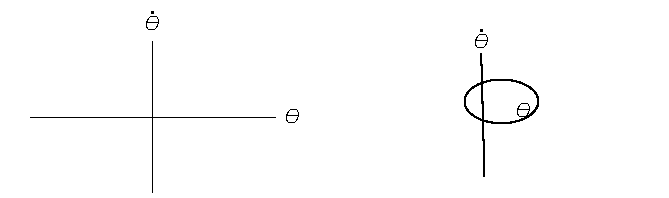
\includegraphics[width=0.5\textwidth]{ode/introduction/pendulum_phase_space}
  \end{center}
  \caption{Two phase spaces for the pendulum.}
  \label{figure pendulum phase space}
\end{figure}


In order to model a process with differential equations it must be 
\textit{deterministic}
\index{deterministic} 
and \textit{differentiable}.  Deterministic means that all past and future
states of the process are determined by its present state.  Each of the 
three examples under consideration are deterministic.  A process is 
differentiable if the phase space is a 
differentiable manifold\footnote{If you don't like the sound of 
``differentiable manifold'', say ``smooth surface'' instead.}
and the evolution of the process is described by differentiable functions.  
Each of our examples are differentiable.

As a side note: the decaying object is deterministic and differentiable 
only when we consider the mass to be continuous.  The object is made up
of atoms.  When individual atoms decay, the mass jumps discontinuously.
With this interpretation, the phase space is the set of points 
$\{ n M : n \in \mathbb{Z}, n \geq 0\}$ where $M$ is the mass of an atom.  The 
phase space is not a differentiable manifold, so the process is not 
differentiable.  Since we don't know exactly when the atoms decay, 
the process is not deterministic.  However, since there are a lot of atoms
it is a good approximation to consider the mass to be continuous.


In addition to being deterministic and differentiable, the phase space of 
a process must be \textit{finite dimensional} in order to be modeled by 
ordinary differential equations.  The decaying mass and the pendulum 
may both be modeled by ordinary differential equations.
Many infinite dimensional processes like the guitar string, may be modeled 
with partial differential equations.


%% CONTINUE HERE


%%=============================================================================
\section{Notation}

The \textit{order} of a differential equation is the order of the highest 
derivative.
\index{order!of a differential equation}
\index{differential equations!order}
The following equations for $y(x)$ are first, second and third order, 
respectively.
\begin{itemize}
\item $y' = x y^2$
\item $y'' + 3 x y' + 2 y = x^2$
\item $y''' = y'' y$
\end{itemize}

The \textit{degree} of a differential equation is the highest power of 
the highest
\index{degree!of a differential equation}
\index{differential equations!degree}
derivative in the equation.  The following equations are first, second 
and third degree, respectively.
\begin{itemize}
\item $y' - 3 y^2 = \sin x$
\item $(y'')^2 + 2 x \cos y = \e^x$
\item $(y')^3 + y^5 = 0$
\end{itemize}
An equation is said to be \textit{linear} if it is linear in the dependent 
variable.
\index{linear differential equations}
\index{differential equations!linear}
\begin{itemize}
\item $y'' \cos x + x^2 y = 0$ is a linear differential equation.
\item $y' + x y^2 = 0$ is a nonlinear differential equation.
\end{itemize}

A differential equation is \textit{homogeneous} if it has no terms that 
are functions of the
\index{homogeneous differential equations}
\index{differential equations!homogeneous}
independent variable alone.  Thus an \textit{inhomogeneous} equation is one in
\index{inhomogeneous differential equations}
\index{differential equations!inhomogeneous}
which there are terms that are functions of the independent variables alone.
\begin{itemize}
\item $y'' + x y + y = 0$ is a homogeneous equation.
\item $y' + y + x^2 = 0$ is an inhomogeneous equation.
\end{itemize}


A first order differential equation may be written in terms of differentials.
Recall that for the function $y(x)$ the differential $\dd y$ is defined
$\dd y = y'(x)\,\dd x$.  Thus the differential equations
\[
y' = x^2 y \quad \mathrm{and} \quad y' + x y^2 = \sin(x)
\]
can be denoted:
\[
\dd y = x^2 y \,\dd x \quad \mathrm{and} \quad 
\dd y + x y^2 \,\dd x = \sin(x) \,\dd x.
\]


A \textit{solution} of a differential equation is a function which when 
substituted into the equation yields an identity.  For example,
$y = x \ln |x|$ is a solution of 
\[
y' - \frac{y}{x} = 1.
\]
We verify this by substituting it into the differential equation.
\[
\ln |x| + 1 - \ln |x| = 1
\]

We can also verify that $y = c \e^x$ is a solution of $y'' - y  = 0$
for any value of the parameter $c$.
\[
c \e^x - c \e^x = 0
\]






%%=============================================================================
\section{Example Problems}



In this section we will discuss physical problems that lead 
to differential equations.


%%---------------------------------------------------------------------------
\subsection{Growth and Decay}



\begin{Example}
  Consider a culture of bacteria in which each bacterium divides 
  once per hour.  Let $n(t) \in \mathbb{N}$ denote the 
  population, let $t$ denote the time in hours and let $n_0$ be the 
  population at time $t = 0$.  The population doubles every hour.  Thus 
  for integer $t$, the population is $n_0 2^t$.  Figure~\ref{figure bacteria1}
  shows two possible populations when there is initially a single 
  bacterium.  In the first plot, each of the bacteria divide at times
  $t = m$ for $m \in \mathbb{N}$.  In the second plot, they divide at 
  times $t = m - 1/2$.  For both plots the population is $2^t$ for 
  integer $t$.

  \begin{figure}[tb!]
    \begin{center}
      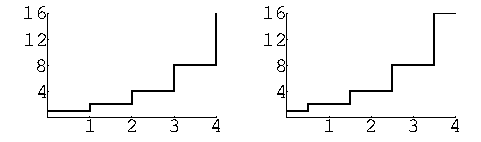
\includegraphics[width=0.6\textwidth]{ode/introduction/bacteria1}
    \end{center}
    \caption{The population of bacteria.}
    \label{figure bacteria1}
  \end{figure}

  We model this problem by considering a continuous population 
  $y(t) \in \mathbb{R}$ which approximates the discrete population.
  In Figure~\ref{figure bacteria8} we first show the population
  when there is initially 8 bacteria.  The divisions of bacteria is 
  spread out over each one second interval.   For integer $t$, the 
  population is $8 \cdot 2^t$.  Next we show the population with a plot of 
  the continuous function $y(t) = 8 \cdot 2^t$.  We see that $y(t)$ is a 
  reasonable approximation of the discrete population.  
  
  \begin{figure}[tb!]
    \begin{center}
      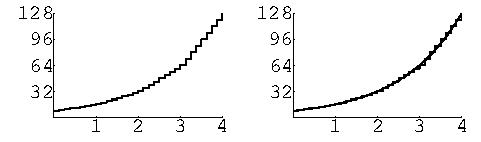
\includegraphics[width=0.6\textwidth]{ode/introduction/bacteria8}
    \end{center}
    \caption{The discrete population of bacteria and a continuous 
      population approximation.}
    \label{figure bacteria8}
  \end{figure}

  In the discrete problem, the growth of the population is proportional 
  to its number; the population doubles every hour.  For the continuous
  problem, we assume that this is true for $y(t)$.  We write this as an 
  equation:
  \[
  y'(t) = \alpha y(t).
  \]
  That is, the rate of change $y'(t)$ in the population is proportional
  to the population $y(t)$, (with constant of proportionality $\alpha$).
  We specify the population at time $t = 0$ with the initial condition:
  $y(0) = n_0$.  Note that $y(t) = n_0 \e^{\alpha t}$ satisfies the problem:
  \[
  y'(t) = \alpha y(t), \quad y(0) = n_0.
  \]
  For our bacteria example, $\alpha = \ln 2$.
\end{Example}


\begin{Result}
  A quantity $y(t)$ whose growth or decay is proportional to $y(t)$
  is modelled by the problem:
  \[
  y'(t) = \alpha y(t), \quad y(t_0) = y_0.
  \]
  Here we assume that the quantity is known at time $t = t_0$.
  $\e^\alpha$ is the factor by which the quantity grows/decays in unit time.
  The solution of this problem is
  $y(t) = y_0 \e^{\alpha (t - t_0)}$.
\end{Result}



\begin{Example}
  Consider a body of radioactive material.  Suppose that we 
  know from physical principles that the rate of decay is proportional to the 
  mass of the body.  At noon the body is 5 grams; by 1:00 PM  it has
  decreased to 4 grams.  When will it be 1 gram?

  Let $y(t)$ be the mass of the body where $t$ measures time in hours and 
  let noon be $t = 0$.  This problem is modelled by:
  \[
  y'(t) = \alpha y(t), \quad y(0) = 5,
  \]
  which has the solution $y(t) = 5 \e^{\alpha t}$.  We substitute in our measurement
  at 1:00 PM to determine the constant of proportionality.
  \begin{gather*}
    4 = 5 \e^{\alpha}
    \\
    \alpha = \ln(4 / 5)
  \end{gather*}
  Thus the solution is $y(t) = 5 (4/5)^t$.  We substitute in $y(t) = 1$ to 
  determine when the body will be 1 gram.
  \begin{gather*}
    1 = 5 (4/5)^t
    \\
    0 = \ln 5 + t \ln(4/5)
    \\
    t = - \frac{ \ln 5 }{ \ln(4/5) } \approx 7.21
  \end{gather*}
  Thus we see that there will be 1 gram remaining at about 7:13 PM.
\end{Example}





%%---------------------------------------------------------------------------
\subsection{1-Dimensional Trajectory Motion}

Consider the vertical motion of an object under the force of gravity.
Let $x$ be the elevation of the object.  The position $x$ and velocity
$\dot{x}$ define its state.  If we neglect air friction, then the 
object experiences an acceleration of $-g$ due to gravity\footnote{
We also assume that the change in the elevation of the object is small enough
to consider the gravitational acceleration to be constant.}.
We write this as a differential equation.
\[
\ddot{x} = - g
\]
We can solve the differential equation by twice integrating with respect 
to $t$.  We will do this in two different ways.  First we take 
indefinite integrals to obtain
\[
x(t) = - \frac{g}{2} t^2 + c_1 t + c_2,
\]
where $c_1$ and $c_2$ are constants of integration.
Suppose that the object has position $x_0$ and velocity $v_0$ at time $t_0$.
We can apply these two constraints, known as \textit{intial conditions},
to determine the constants of integration.
\begin{gather*}
  x(t_0) = x_0 \quad \Rightarrow \quad - \frac{g}{2} t_0^2 + c_1 t_0 + c_2 = x_0
  \\
  \dot{x}(t_0) = v_0 \quad \Rightarrow \quad -g t_0 + c_1 = v_0
  \\
  x(t) = - \frac{g}{2} t^2 + (g t_0 + v_0) t 
  - \frac{g}{2} t_0^2 - t_0 v_0 + x_0
\end{gather*}
\begin{equation}
  \label{equation 1D trajectory solution}
  x(t) = - \frac{g}{2} (t - t_0)^2 + v_0 (t - t_0) + x_0
\end{equation}

Another approach is to take definite integrals from $t_0$ to $t$.
\begin{gather*}
  \ddot{x} = - g
  \\
  \int_{t_0}^t \ddot{x}(\tau) \,\dd \tau = \int_{t_0}^t -g \,\dd \tau 
  \\
  \dot{x}(t) - \dot{x}(t_0) = - g (t - t_0)
  \\
  \int_{t_0}^t (\dot{x}(\tau) - v_0) \,\dd \tau = \int_{t_0}^t -g (\tau - t_0) \,\dd \tau 
  \\
  x(t) - x(t_0) - v_0 (t - t_0) = - \frac{g}{2} (t - t_0)^2
  \\
  x(t) = - \frac{g}{2} (t - t_0)^2 + v_0 (t - t_0) + x_0
\end{gather*}
We obtain the same result either way.  For the latter method, the initial
conditions are introduced as we evaluate the definite integrals.

There are a number of ways to plot the motion of the trajectory.  First 
consider an object dropped at $t = 0$ from an initial height of $x_0$.
In the first plot in Figure~\ref{figure trajectory 1d tx} we show the 
elevation versus time.  Then consider an object projected upward at $t = 0$
with an initial velocity of $v_0$.  These trajectories are shown in the
second plot.

\begin{figure}[tb!]
  \begin{center}
    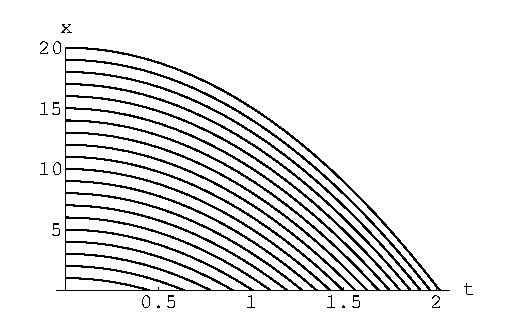
\includegraphics[width=0.49\textwidth]{ode/introduction/trajectory_1d_tx_x0}
    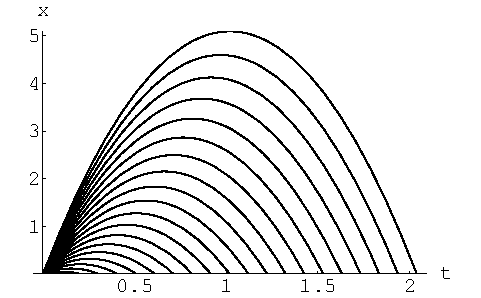
\includegraphics[width=0.49\textwidth]{ode/introduction/trajectory_1d_tx_v0}
  \end{center}
  \caption{Trajectories of objects dropped from an initial height and 
    projected upward from zero height.}
  \label{figure trajectory 1d tx}
\end{figure}

We can also plot these trajectories in phase space.  (See 
Figure~\ref{figure trajectory 1d xxd}.)  These plots show the evolution of the 
state of the object.

\begin{figure}[tb!]
  \begin{center}
    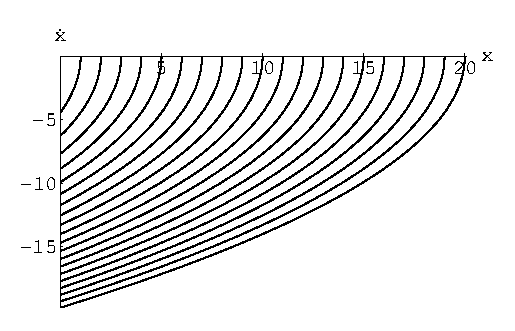
\includegraphics[width=0.49\textwidth]{ode/introduction/trajectory_1d_xxd_x0}
    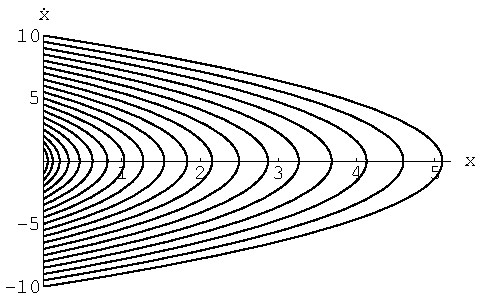
\includegraphics[width=0.49\textwidth]{ode/introduction/trajectory_1d_xxd_v0}
  \end{center}
  \caption{The trajectories plotted in phase space.}
  \label{figure trajectory 1d xxd}
\end{figure}


Note that the time factors in the solution subject to the initial conditions 
(Equation~\ref{equation 1D trajectory solution})
all appear as $(t - t_0)$.  This is not mere coincidence.  The equation
of motion $\ddot{x} = - g$ is \textit{shift invariant} with respect to $t$.
\index{shift invariant}
This means that the equation is unchanged under the transformation 
$t \to t - t_0$.   We can state this in physical terms: the motion of the 
object does not depend on the starting time.  The object will fall in 
the same manner whether we drop it today, tomorrow or next week.  Thus, 
without loss of generality, we can take the starting time to be $t = 0$.
In this case the solution is
\[
x(t) = - \frac{g}{2} t^2 + v_0 t + x_0
\]
If we change the starting time to $t = 42$, we just make the 
substitution $t \to t - 42$ to obtain the solution for the new 
starting time.
\[
x(t) = - \frac{g}{2} (t - 42)^2 + v_0 (t - 42) + x_0
\]



%%---------------------------------------------------------------------------
\subsection{2-Dimensional Trajectory Motion}

Consider the 2-D motion of an object under the force of gravity.
Let $(x,y)$ be the position of the object.  The position $(x,y)$ and velocity
$(\dot{x}, \dot{y})$ define its state.  The 
object experiences an acceleration of $-g$ in the vertical direction 
due to gravity.  There is no applied force in the horizontal direction.
We write these relations as differential equations.
\[
\ddot{x} = - g, \quad \ddot{y} = 0
\]

\begin{Exercise}
  \label{exercise hunter monkey}
  A hunter aims his rifle exactly at a monkey hanging from a tree branch.
  At the same time the hunter pulls the trigger, the monkey lets go of
  the branch.  Does the bullet hit the monkey?  Solve the differential
  equations of motion to find out.
  
  \hintsolution{hunter monkey}
\end{Exercise}




%%---------------------------------------------------------------------------
\subsection{Mass on a Spring}


\begin{figure}[tb!]
  \begin{center}
    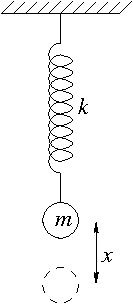
\includegraphics[width=0.15\textwidth]{ode/introduction/mass_on_spring}
  \end{center}
  \caption{A mass on a spring.}
  \label{figure mass on spring}
\end{figure}

Consider the vertical motion of a ball of mass $m$ suspended from an 
ideal spring\footnote{An ideal spring is massless and obeys Hooke's law.}.  
(See Figure~\ref{figure mass on spring}.)  Let $x$ be the displacement 
from the equilibrium position.  Hooke's law 
\index{Hooke's law} 
states that the force from the spring is directly proportional to this 
displacement.
\[
\mathrm{force} = - k \ \mathrm{displacement}
\]
$k$ is called the spring constant.  The force applied to the mass is equal
to the derivative of its momentum $m \dot{x}$.  We use this to obtain a 
differential equation for the motion.
\begin{gather*}
  \frac{\dd}{\dd t}(m \dot{x}) = - k x
  \\
  \ddot{x} + \frac{k}{m} x = 0
\end{gather*}

Now we make the unmotivated substitution $\omega_0 := k / m$.  The equation becomes
\begin{equation}
  \label{ddot x + w02 x = 0}
\ddot{x} + \omega_0^2 x = 0.
\end{equation}

\begin{Exercise}
  \label{exercise mass on spring solutions}
  Verify that both
  \[
  x = a \cos( \omega_0 t ) + b \sin( \omega_0 t )
  \]
  and
  \[
  x = A \sin( \omega_0 t + \phi )
  \]
  satisfy Equation~\ref{ddot x + w02 x = 0} where $a$, $b$, $A$, and $\phi$ are 
  arbitrary constants.  Are these two solutions equivalent?
  
  \hintsolution{mass on spring solutions}
\end{Exercise}

The motion of the mass is called \textit{simple harmonic motion}.
\index{simple harmonic motion}
$\omega_0$ is the frequency of the oscillations; $A$ is the amplitude.  The 
frequency increases with increasing stiffness of the spring and decreasing
mass of the object.





%%---------------------------------------------------------------------------
\subsection{Pendulum}

\begin{figure}[tb!]
  \begin{center}
    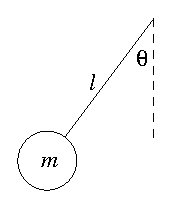
\includegraphics[width=0.15\textwidth]{ode/introduction/pendulum}
  \end{center}
  \caption{A pendulum.}
  \label{figure pendulum}
\end{figure}

Consider the motion of a pendulum in a plane.  
(See Figure~\ref{figure pendulum}.)  The head of the pendulum has mass $m$.
The rod is massless and has length $l$.  Let $\theta$ be the angular displacement
from the vertical resting position.  The angular velocity is $\dot{\theta}$.
The angular momentum is $l^2 m \dot{\theta}$.  The pendulum moves under the 
force of gravity, $g$ in the downward direction.  This produces a 
torque of $- l m g \sin \theta$.  We equate the torque with the derivative 
of the angular momentum to obtain the differential equation of the 
motion.
\begin{gather*}
  \frac{ \dd }{ \dd t } ( l^2 m \dot{\theta} ) = - l m g \sin \theta
  \\
  \ddot{\theta} + \frac{g}{l} \sin \theta = 0
\end{gather*}
For small $\theta$, $\sin \theta \approx \theta$.  Thus for small oscillations, the motion 
is approximately modelled by an equation for simple harmonic motion:
\[
\ddot{\theta} + \frac{g}{l} \theta = 0.
\]
The frequency for small oscillations is $\omega \approx \sqrt{ g / l }$.


%% CONTINUE





\raggedbottom
%%============================================================================
\exercises{
\pagebreak
\flushbottom
\section{Exercises}




\raggedbottom
}
%%============================================================================
\pagebreak
\flushbottom
\section{Hints}
\hints{

\begin{Hint}
  \label{hint mass on spring solutions}
  Use a trigonometric identity (Appendix~\ref{trigonometric_identities}) 
  to show that the solutions are equivalent.
\end{Hint}

\begin{Hint}
  \label{hint hunter monkey}
  This is a 2-D problem.  The bullet and the monkey move in the vertical 
  plane defined by the hunter and the initial position of the monkey.  Let 
  the hunter be at the origin and fire the rifle at $t = 0$.  Let the 
  initial position of the monkey be a distance $d$ from the hunter and
  and angle $\theta$ from the horizontal axis.  Let the bullet travel with 
  a speed of $v$.  Let $(x,y)$ be the
  position of the bullet and $(\xi,\psi)$ be the position of the monkey.
  Find the positions as a function of time and then see if there
  is a solution of $(x(t), y(t)) = (\xi(t), \psi(t))$ for some positive time.
\end{Hint}





\raggedbottom
}
%%============================================================================
\pagebreak
\flushbottom
\section{Solutions}
\solutions{

\begin{Solution}
  \label{solution mass on spring solutions}
  Consider the first proposed solution.
  \begin{gather*}
    x = a \cos( \omega_0 t ) + b \sin( \omega_0 t )
    \\
    \ddot{x} = - a \omega_0^2 \cos( \omega_0 t ) - b \omega_0^2 \sin( \omega_0 t )
  \end{gather*}
  We substitute it into the differential equation and obtain an identity.
  \begin{gather*}
    \ddot{x} + \omega_0^2 x = 0
    \\
    \left( - a \omega_0^2 \cos( \omega_0 t ) - b \omega_0^2 \sin( \omega_0 t ) \right)
    + \omega_0^2 \left( a \cos( \omega_0 t ) + b \sin( \omega_0 t ) \right) = 0
    \\
    0 = 0
  \end{gather*}

  Likewise with the second proposed solution.
  \begin{gather*}
    x = A \sin( \omega_0 t + \phi )
    \\
    \ddot{x} = - A \omega_0^2 \sin( \omega_0 t + \phi )
  \end{gather*}
  We substitute it into the differential equation and obtain an identity.
  \begin{gather*}
    \ddot{x} + \omega_0^2 x = 0
    \\
    \left( - A \omega_0^2 \sin( \omega_0 t + \phi ) \right)
    + \omega_0^2 \left( A \sin( \omega_0 t + \phi ) \right) = 0
    \\
    0 = 0
  \end{gather*}

  The two solutions are equivalent.  To demonstrate this 
  we use trigonometric identities
  to change the form of the second solution.
  \[
  A \sin( \omega_0 t + \phi ) 
  = A \sin \phi \cos( \omega_0 t ) + A \cos \phi \sin( \omega_0 t )
  \]
  By equating the two solutions we see how the parameters are related.
  \[
  a = A \sin \phi, \quad b = A \cos \phi
  \]
  We can also write $A$ and $\phi$ in terms of $a$ and $b$.
  First we square and add the equations to determine $A$.
  \begin{gather*}
    a^2 + b^2 = A^2 (\sin^2 \phi + \cos^2 \phi)
    \\
    A = \sqrt{ a^2 + b^2 }
  \end{gather*}
  Then we determine $\phi$.
  \begin{gather*}
    b = \sqrt{ a^2 + b^2 } \cos \phi
    \\
    \phi = \arccos \left( \frac{ b }{ \sqrt{ a^2 + b^2 } } \right)
  \end{gather*}
\end{Solution}





\begin{Solution}
  \label{solution hunter monkey}
  This is a 2-D problem.  The bullet and the monkey move in the vertical 
  plane defined by the hunter and the initial position of the monkey.  Let 
  the hunter be at the origin and fire the rifle at $t = 0$.  Let the 
  initial position of the monkey be a distance $d$ from the hunter and
  and angle $\theta$ from the horizontal axis.  Let the bullet travel with 
  a speed of $v$.  We assume the speed is sufficient for the bullet to 
  reach the monkey before either hits the ground.  Let $(x,y)$ be the
  position of the bullet and $(\xi,\psi)$ be the position of the monkey.
  We will find the positions as a function of time and then see if there
  is a solution of $(x(t), y(t)) = (\xi(t), \psi(t))$.

  First we write the differential equations and the initial conditions.
  (We know that $\xi(t) = d \cos \theta$ because the monkey falls vertically.)
  \begin{gather*}
    \ddot{x} = 0, \quad x(0) = 0,\ \dot{x}(0) = v \cos \theta
    \\
    \ddot{y} = - g, \quad y(0) = 0,\ \dot{y}(0) = v \sin \theta
    \\
    \ddot{\psi} = - g, \quad y(0) = d \sin \theta,\ \dot{y}(0) = 0
  \end{gather*}
  We can solve the differential equation for $x$ by integrating.
  \begin{gather*}
    \ddot{x} = 0
    \\
    \int_0^t \ddot{x}(\tau) \,\dd \tau = 0
    \\
    \dot{x}(t) - \dot{x}(0) = 0
    \\
    \dot{x}(t) = v \cos \theta
    \\
    \int_0^t \dot{x}(\tau) \,\dd \tau = \int_0^t v \cos \theta \,\dd \tau
    \\
    x(t) - x(0) = v t \cos \theta
    \\ 
    x(t) = v t \cos \theta
  \end{gather*}
  Equation~\ref{equation 1D trajectory solution} gives the solution for
  $y(t)$ and $\psi(t)$.
  \begin{gather*}
    y(t) = - \frac{g}{2} t^2 + v t \sin \theta
    \\
    \psi(t) = - \frac{g}{2} t^2 + d \sin \theta
  \end{gather*}

  Now we determine if there is a time when the positions of the bullet and
  the monkey coincide.  First we solve for the horizontal position.
  \begin{gather*}
    x(t) = \xi(t)
    \\
    v t \cos \theta = d \cos \theta
    \\
    t = \frac{d}{t}
  \end{gather*}
  Then we solve for the vertical position.
  \begin{gather*}
    y(t) = \psi(t)
    \\
    - \frac{g}{2} t^2 + v t \sin \theta = - \frac{g}{2} t^2 + d \sin \theta
    \\
    t = \frac{d}{t}
  \end{gather*}
  Thus we see that the bullet hits the monkey at $t = d / v$.
\end{Solution}


\raggedbottom
}

\flushbottom


%% CONTINUE
%% Show that the solutions to a first order differential equation are a 
%% one-parameter family.




%%=============================================================================
%%=============================================================================
\chapter{First Order Differential Equations}
\label{chapter_foo}
\index{differential equations!first order}

Don't show me your technique.  Show me your heart.

\begin{flushright}
  -Tetsuyasu Uekuma
\end{flushright}








%%=============================================================================
\section{One Parameter Families of Functions}



Consider the equation:
\begin{equation}
  \label{equation F(x,y(x),c)=0}
  F(x, y(x), c) = 0,
\end{equation}
which implicitly defines a one-parameter family of functions $y(x;c)$.
Here $y$ is a function of the variable $x$ and the parameter $c$.
For simplicity, we will write $y(x)$ and not explicitly show the 
parameter dependence.


\begin{Example}
  The equation $y = c x$ defines family of lines with slope $c$, passing
  through the origin.  The equation $x^2 + y^2 = c^2$ defines circles
  of radius $c$, centered at the origin.

  Consider a 
  \hyperref[chapter spherical chicken]{chicken}
  dropped from 
  a height $h$.  The elevation $y$ of the chicken at time $t$ after 
  its release is $y(t) = h - g t^2$, where $g$ is the acceleration due 
  to gravity.  This is family of functions for the parameter $h$.
\end{Example}


It turns out that the general solution of any first order differential
equation is a one-parameter family of functions.  This is not easy to
prove.  However, it is easy to verify the converse.
We differentiate Equation~\ref{equation F(x,y(x),c)=0} with respect 
to $x$.
\[
F_x + F_y y' = 0
\]
(We assume that $F$ has a non-trivial dependence on $y$, that is $F_y
\neq 0$.)  This gives us two equations involving the independent
variable $x$, the dependent variable $y(x)$ and its derivative and the
parameter $c$.  If we algebraically eliminate $c$ between the two
equations, the eliminant will be a first order differential equation
for $y(x)$.  Thus we see that every one-parameter family of functions
$y(x)$ satisfies a first order differential equation.  This $y(x)$ is
the \textit{primitive} of the differential equation.  Later we will
discuss why $y(x)$ is the \textit{general solution} of the
differential equation.
%% CONTINUE  add a link for ``Later'' if I do show that.




\begin{Example}
  Consider the family of circles of radius $c$ centered about the origin.
  \[
  x^2 + y^2 = c^2
  \]
  Differentiating this yields:
  \[
  2 x + 2 y y' = 0.
  \]
  It is trivial to eliminate the parameter and obtain a differential equation
  for the family of circles.
  \[
  x + y y' = 0
  \]
  We can see the geometric meaning in this equation by writing it in the 
  form:
  \[
  y' = - \frac{x}{y}.
  \]
  For a point on the circle, the slope of the tangent $y'$
  is the negative of the cotangent of the angle $x/y$.
  (See Figure~\ref{figure circle tangent}.)
  \begin{figure}[tb!]
    \begin{center}
      %% CONTINUE Fix this graphic.
      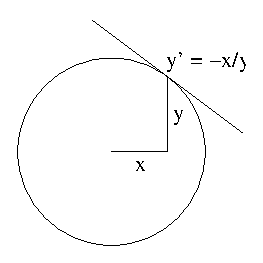
\includegraphics[width=0.2\textwidth]{ode/first_order/circle_tangent}
    \end{center}
    \caption{A circle and its tangent.}
    \label{figure circle tangent}
  \end{figure}
\end{Example}




\begin{Example}
  Consider the one-parameter family of functions:
  \[
  y(x) = f(x) + c g(x),
  \]
  where $f(x)$ and $g(x)$ are known functions.  The derivative is
  \[
  y' = f' + c g'.
  \]
  We eliminate the parameter.
  \begin{gather*}
    g y' - g' y = g f' - g' f \\
    y' - \frac{g'}{g} y = f' - \frac{g' f}{g}
  \end{gather*}
  Thus we see that $y(x) = f(x) + c g(x)$ satisfies a first order 
  \textit{linear} differential equation.  Later we will prove the 
  converse: the general solution of a first order linear differential
  equation has the form: $y(x) = f(x) + c g(x)$.
\end{Example}



We have shown that every one-parameter family of functions satisfies a first 
order differential equation.  We do not prove it here, but the converse 
is true as well.


\begin{Result}
  Every first order differential equation has a one-parameter family of 
  solutions $y(x)$ defined by an equation of the form:
  \[
  F(x, y(x); c) = 0.
  \]
  This $y(x)$ is called the \textit{general solution}.  If the
  equation is linear then the general solution expresses the
  totality of solutions of the differential equation.  If the
  equation is nonlinear, there may be other special \textit{singular
    solutions}, which do not depend on a parameter.
\end{Result}



This is strictly an existence result.  It does not say that the general 
solution of a first order differential equation can be determined by some
method, it just says that it exists.  There is no method for solving 
the general first order differential equation.  However, there are some
special forms that are soluble.  We will devote the rest of this chapter 
to studying these forms.





%%=============================================================================
\section{Integrable Forms}


In this section we will introduce a few forms of differential equations
that we may solve through integration.


%%-----------------------------------------------------------------------------
\subsection{Separable Equations}
\index{differential equations!separable}
\index{separable equations}




Any differential equation that can written in the form
\[ 
P(x) + Q(y) y' = 0
\]
is a \textit{separable equation}, (because the dependent and independent
variables are separated).  We can obtain an implicit solution by integrating
with respect to $x$.
\begin{gather*}
  \int P(x) \,\dd x + \int Q(y) \frac{\dd y}{\dd x} \,\dd x = c 
  \\
  \int P(x) \,\dd x + \int Q(y) \,\dd y = c
\end{gather*}



\begin{Result}
  The separable equation $P(x) + Q(y) y' = 0$ may be solved by integrating
  with respect to $x$.  The general solution is
  \[ 
  \int P(x) \,\dd x + \int Q(y) \,\dd y = c.
  \]
\end{Result}



\begin{Example}
  Consider the differential equation $y' = x y^2$.
  We separate the dependent and independent variables and integrate to find
  the solution.
  \begin{gather*}
    \frac{\dd y}{\dd x} = x y^2 
    \\
    y^{-2}\,\dd y = x\,\dd x 
    \\
    \int y^{-2}\,\dd y = \int x \,\dd x + c 
    \\
    -y^{-1} = \frac{x^2}{2} + c 
    \\
    \boxed{
      y = - \frac{1}{x^2/2 + c}
      }
  \end{gather*}
\end{Example}







\begin{Example}
  The equation $y' = y - y^2$ is separable.
  \[
  \frac{y'}{y - y^2} = 1
  \]
  We expand in partial fractions and integrate.
  \begin{gather*}
    \left( \frac{1}{y} - \frac{1}{y-1} \right) y' = 1 
    \\
    \ln |y| - \ln |y - 1| = x + c
  \end{gather*}
  We have an implicit equation for $y(x)$.  Now we solve for $y(x)$.
  \begin{gather*}
    \ln \left| \frac{y}{y-1} \right| = x + c 
    \\
    \left| \frac{y}{y-1} \right| = \e^{x+c} 
    \\
    \frac{y}{y-1} = \pm \e^{x+c} 
    \\
    \frac{y}{y-1} = c \e^x 
    \footnote{Here we have substituted $c$ for $\pm \e^c$.}
    \\
    y = \frac{c \e^x}{c \e^x - 1}
    \\
    \boxed{
      y = \frac{1}{1 + c \e^{x}}
      }
  \end{gather*}
\end{Example}










%%=============================================================================
\subsection{Exact Equations}
\index{differential equations!exact}
\index{exact equations}



Any first order ordinary differential equation of the first degree can 
be written as the total differential equation,
\[
P(x, y) \,\dd x + Q(x, y) \,\dd y = 0.
\]
If this equation can be integrated directly, that is if there is a primitive,
$u(x, y)$, such that 
\[
d u = P \,\dd x + Q \,\dd y,
\]
then this equation is called \textit{exact}.
The (implicit) solution of the differential equation is 
\[
u(x, y) = c,
\]
where $c$ is an arbitrary constant.  
Since the differential of a function, $u(x, y)$, is
\[
\dd u \equiv \frac{\partial u}{\partial x} \,\dd x + \frac{\partial u}{\partial y} \,\dd y,
\]
$P$ and $Q$ are the partial derivatives of $u$:
\[
P(x, y) = \frac{\partial u}{\partial x}, \qquad 
Q(x, y) = \frac{\partial u}{\partial y}.
\]

In an alternate notation, the differential equation
\begin{equation}
  \label{first_order_first_degree}
  P(x, y) + Q(x, y) \frac{\dd y}{\dd x} = 0,
\end{equation}
is exact if there is a primitive $u(x, y)$ such that
\[
\frac{\dd u}{\dd x} \equiv \frac{\partial u}{\partial x} + \frac{\partial u}{\partial y} \frac{\dd y}{\dd x}
= P(x, y) + Q(x, y) \frac{\dd y}{\dd x}.
\]
The solution of the differential equation is $u(x, y) = c$.





\begin{Example}
  \[
  x + y \frac{\dd y}{\dd x} = 0
  \]
  is an exact differential equation since
  \[
  \frac{\dd}{\dd x} \left( \frac{1}{2} (x^2 + y^2) \right) = x + y \frac{\dd y}{\dd x}
  \]
  The solution of the differential equation is
  \[
  \frac{1}{2} (x^2 + y^2) = c.
  \]
\end{Example}




\begin{Example}
  \label{product_rule_exact_equation},
  Let $f(x)$ and $g(x)$ be known functions.
  \[
  g(x) y' + g'(x) y = f(x)
  \]
  is an exact differential equation since
  \[
  \frac{\dd}{\dd x} \left( g(x) y(x) \right) = g y' + g' y.
  \]
  The solution of the differential equation is
  \begin{gather*}
    g(x) y(x) = \int f(x)\,\dd x + c \\
    y(x) = \frac{1}{g(x)} \int f(x) \,\dd x + \frac{c}{g(x)}.
  \end{gather*}
\end{Example}



\paragraph{A necessary condition for exactness.}
The solution of the exact equation $P + Q y' = 0$ is $u = c$
where $u$ is the primitive of the equation,  $\frac{\dd u}{\dd x} = P + Q y'$.
At present the only method we have for determining the primitive is 
guessing.   This is fine for simple equations, but for more difficult
cases we would like a method more concrete than divine inspiration.  As a
first step toward this goal we determine a criterion for determining if
an equation is exact.

Consider the exact equation,
\[
P + Q y' = 0,
\]
with primitive $u$, where we assume that the functions $P$ and $Q$ are 
continuously differentiable.  Since the mixed partial derivatives of $u$ 
are equal,
\[
\frac{\partial^2 u}{\partial x \partial y} = \frac{\partial^2 u}{\partial y \partial x},
\]
a necessary condition for exactness is
\[
\frac{\partial P}{\partial y} = \frac{\partial Q}{\partial x}.
\]



\paragraph{A sufficient condition for exactness.}
This necessary condition for exactness is also a sufficient condition.
We demonstrate this by deriving the general solution of 
(\ref{first_order_first_degree}).  Assume that $P + Q y' = 0$
is not necessarily exact, but satisfies the condition $P_y = Q_x$.
If the equation has a primitive, 
\[
\frac{\dd u}{\dd x} \equiv \frac{\partial u}{\partial x} + \frac{\partial u}{\partial y} \frac{\dd y}{\dd x}
= P(x, y) + Q(x, y) \frac{\dd y}{\dd x},
\]
then it satisfies
\begin{equation}
  \label{ux=p_uy=q}
  \frac{\partial u}{\partial x} = P, \qquad \frac{\partial u}{\partial y} = Q.
\end{equation}
Integrating the first equation of (\ref{ux=p_uy=q}), we see that the 
primitive has the form
\[
u(x, y) = \int_{x_0}^x P(\xi, y) \,\dd \xi + f(y),
\]
for some $f(y)$.
Now we substitute this form into the second equation of (\ref{ux=p_uy=q}).
\begin{gather*}
  \frac{\partial u}{\partial y} = Q(x, y) \\
  \int_{x_0}^x P_y(\xi, y) \,\dd \xi + f'(y) = Q(x, y) \\
  \intertext{Now we use the condition $P_y = Q_x$.}
  \int_{x_0}^x Q_x(\xi, y) \,\dd \xi + f'(y) = Q(x, y) \\
  Q(x,y) - Q(x_0, y) + f'(y) = Q(x, y) \\
  f'(y) = Q(x_0, y) \\
  f(y) = \int_{y_0}^y Q(x_0, \psi) \,\dd \psi
\end{gather*}
Thus we see that 
\[
u = \int_{x_0}^x P(\xi, y) \,\dd \xi + \int_{y_0}^y Q(x_0, \psi) \,\dd \psi
\]
is a primitive of the derivative; the equation is exact.  The solution of
the differential equation is
\[
\int_{x_0}^x P(\xi, y) \,\dd \xi + \int_{y_0}^y Q(x_0, \psi) \,\dd \psi = c.
\]
Even though there are three arbitrary constants: $x_0$, $y_0$ and $c$, 
the solution is a one-parameter family.  This is because changing 
$x_0$ or $y_0$ only changes the left side by an additive constant.




\begin{Result}
  Any first order differential equation of the first degree can be written
  in the form
  \[
  P(x, y) + Q(x, y) \frac{\dd y}{\dd x} = 0.
  \]
  This equation is exact if and only if
  \[
  P_y = Q_x.
  \]
  In this case the solution of the differential equation is given by
  \[
  \int_{x_0}^x P(\xi, y) \,\dd \xi 
  + \int_{y_0}^y Q(x_0, \psi) \,\dd \psi = c.
  \]
\end{Result}





%% CONTINUE: cover integrating factors.






%% Solve first order equations by inspection.
\begin{Exercise}
  \label{exercise gygyf}
  Solve the following differential equations by inspection.  That is, group 
  terms into exact derivatives and then integrate. 
  $f(x)$ and $g(x)$ are known functions.
  \begin{enumerate}
    %%
  \item $\frac{y'(x)}{y(x)} = f(x)$
    %%
  \item $y^\alpha(x) y'(x) = f(x)$
    %%
  \item $\frac{y'}{\cos x} + y \frac{\tan x}{\cos x} = \cos x$
  \end{enumerate}

  \hintsolution{gygyf}
\end{Exercise}























%%-----------------------------------------------------------------------------
\subsection{Homogeneous Coefficient Equations}
\index{differential equations!homogeneous coefficient}
\index{homogeneous coefficient equations}
\index{homogeneous functions}
\index{Euler's theorem}



Homogeneous coefficient, first order differential equations form another class
of soluble equations.  We will find that a change of dependent variable 
will make such equations separable or we can determine an integrating factor 
that will make such equations exact.  First we define homogeneous functions.



\paragraph{Euler's Theorem on Homogeneous Functions.}
The function $F(x,y)$ is \textit{homogeneous of degree} $n$ if
\[
F(\lambda x,\lambda y) = \lambda^n F(x,y).
\]
From this definition we see that
\[
F(x,y) = x^n F \left( 1, \frac{y}{x} \right).
\]
(Just formally substitute $1/x$ for $\lambda$.)
For example, 
\[
x y^2, \qquad
\frac{x^2 y+ 2 y^3}{x + y}, \qquad
x \cos(y/x)
\]
are homogeneous functions of orders 3, 2 and 1, respectively.


Euler's theorem for a homogeneous function of order $n$ is:
\[
x F_x + y F_y = n F.
\]
To prove this, we define $\xi = \lambda x$, $\psi = \lambda y$.
From the definition of homogeneous functions, we have
\[
F(\xi, \psi) = \lambda^n F(x,y).
\]
We differentiate this equation with respect to $\lambda$.
\begin{gather*}
  \frac{\partial F(\xi,\psi)}{\partial \xi} \frac{\partial \xi}{\partial \lambda}
  + \frac{\partial F(\xi,\psi)}{\partial \psi} \frac{\partial \psi}{\partial \lambda}
  = n \lambda^{n-1} F(x,y) \\
  x F_\xi + y F_\psi = n \lambda^{n-1} F(x,y)
\end{gather*}
Setting $\lambda = 1$, (and hence $\xi = x$, $\psi = y$),
proves Euler's theorem.


\begin{Result}
  \textbf{Euler's Theorem on Homogeneous Functions.}
  If $F(x, y)$ is a homogeneous function of degree $n$, then
  \[
  x F_x + y F_y = n F.
  \]
\end{Result}








\paragraph{Homogeneous Coefficient Differential Equations.}
If the coefficient functions $P(x, y)$ and $Q(x, y)$ are homogeneous of 
degree $n$ then the differential equation,
\begin{equation}
  \label{homogeneous differential equation}
  P(x, y) + Q(x, y) \frac{\dd y}{\dd x} = 0,
\end{equation}
is called a \textit{homogeneous coefficient equation}.  They are often
referred to simply as \textit{homogeneous equations}.   



\paragraph{Transformation to a Separable Equation.}
We can write the homogeneous equation in the form,
\begin{gather*}
  x^n P \left(1, \frac{y}{x} \right) 
  + x^n Q \left(1, \frac{y}{x} \right) \frac{\dd y}{\dd x} = 0, 
  \\
  P \left(1, \frac{y}{x} \right) 
  + Q \left(1, \frac{y}{x} \right) \frac{\dd y}{\dd x} = 0.
\end{gather*}
This suggests the change of dependent variable $u(x) = \frac{y(x)}{x}$.
\[
P(1, u) + Q(1, u) \left( u + x \frac{\dd u}{\dd x} \right) = 0
\]
This equation is separable.
\begin{gather*}
  P(1, u) + u Q(1, u) + x Q(1, u) \frac{\dd u}{\dd x} = 0 
  \\
  \frac{1}{x} + \frac{Q(1, u)}{P(1, u) + u Q(1, u)} \frac{\dd u}{\dd x} = 0 
  \\
  \ln |x| + \int \frac{1}{u + P(1, u) / Q(1, u)} \,\dd u = c 
  \\
  \intertext{By substituting $\ln |c|$ for $c$, we can write this in a 
    simpler form.}
  \int \frac{1}{u + P(1, u) / Q(1, u)} \,\dd u = \ln \left| \frac{c}{x} \right|.
\end{gather*}


\paragraph{Integrating Factor.}
One can show that
\[
\mu(x,y) = \frac{1}{x P(x,y) + y Q(x,y)}
\]
is an integrating factor for the Equation~
\ref{homogeneous differential equation}.  The proof of this is left as 
an exercise for the reader.  (See Exercise~
\ref{exercise integrating factor homogeneous}.)





\begin{Result}
  \textbf{Homogeneous Coefficient Differential Equations.}
  If $P(x, y)$ and $Q(x, y)$ are homogeneous functions of degree $n$, then
  the equation 
  \[
  P(x, y) + Q(x, y) \frac{\dd y}{\dd x} = 0
  \]
  is made separable by the change of independent variable 
  $u(x) = \frac{y(x)}{x}$.  The solution is determined by
  \[
  \int \frac{1}{u + P(1, u) / Q(1, u)} \,\dd u = \ln \left| \frac{c}{x} \right|.
  \]
  Alternatively, the homogeneous equation can be made exact with the 
  integrating factor
  \[
  \mu(x,y) = \frac{1}{x P(x,y) + y Q(x,y)}.
  \]
\end{Result}








\begin{Example}
  Consider the homogeneous coefficient equation
  \[
  x^2 - y^2 + x y \frac{\dd y}{\dd x} = 0.
  \]
  The solution for $u(x) = y(x) / x$ is determined by
  \begin{gather*}
    \int \frac{1}{u + \frac{1 - u^2}{u} }\,\dd u = \ln \left| \frac{c}{x} \right| 
    \\
    \int u \,\dd u = \ln \left| \frac{c}{x} \right| 
    \\
    \frac{1}{2} u^2 = \ln \left| \frac{c}{x} \right| 
    \\
    u = \pm \sqrt{2 \ln |c/x|}
  \end{gather*}
  Thus the solution of the differential equation is
  \[
  \boxed{
    y = \pm x \sqrt{2 \ln |c/x|}
    }
  \]
\end{Example}




%% CONTINUE: cover equations that are homogeneous and exact.
%% CONTINUE: integrating factor for homogeneous equations. 






%% \mu(x,y) = \frac{1}{x M(x,y) + y N(x,y)}
\begin{Exercise}
  \label{exercise integrating factor homogeneous}
  Show that
  \[
  \mu(x,y) = \frac{1}{x P(x,y) + y Q(x,y)}
  \]
  is an integrating factor for the homogeneous equation,
  \[
  P(x,y) + Q(x,y) \frac{\dd y}{\dd x} = 0.
  \]

  \hintsolution{integrating factor homogeneous}
\end{Exercise}







%% $d y / d t = f(y / t)$.
\begin{Exercise}[mathematica/ode/first\_order/exact.nb]
  \label{exercise dydt = f(y/t)}
  Find the general solution of the equation 
  \[
  \frac{\dd y}{\dd t} = 2 \frac{y}{t} + \left( \frac{y}{t} \right)^2.
  \]
  
  \hintsolution{dydt = f(y/t)}
\end{Exercise}











%%=============================================================================
\section{The First Order, Linear Differential Equation}
\index{differential equations!first order}



%%-----------------------------------------------------------------------------
\subsection{Homogeneous Equations}




The first order, linear, homogeneous equation has the form
\[ 
\frac{\dd y}{\dd x} + p(x) y = 0.
\]
Note that if we can find one solution, then any constant times that solution
also satisfies the equation.  In fact, all the solutions of this 
equation differ only by multiplicative constants.
We can solve any equation of this type because it is separable.
\begin{gather*}
  \frac{y'}{y} = - p(x) 
  \\
  \ln |y| = - \int p(x) \,\dd x + c 
  \\
  y = \pm \e^{- \int p(x) \,\dd x + c} 
  \\
  y = c \e^{- \int p(x) \,\dd x}
\end{gather*}




\begin{Result}
  \textbf{First Order, Linear Homogeneous Differential Equations.}
  The first order, linear, homogeneous differential equation,
  \[ 
  \frac{\dd y}{\dd x} + p(x) y = 0,
  \]
  has the solution
  \begin{equation}
    \label{first order linear homogeneous}
    y = c \e^{- \int p(x) \,\dd x}.
  \end{equation}
  The solutions differ by multiplicative constants.  
\end{Result}







\begin{Example}  
  Consider the equation
  \[ 
  \frac{\dd y}{\dd x} + \frac{1}{x} y = 0.
  \]
  We use Equation~\ref{first order linear homogeneous} to determine 
  the solution.
  \begin{gather*}
    y(x) = c \e^{ - \int 1/x \,\dd x }, \quad \mathrm{for}\ x \neq 0
    \\
    y(x) = c \e^{ - \ln |x| }
    \\
    y(x) = \frac{c}{|x|}
    \\
    \boxed{
      y(x) = \frac{c}{x}
      }
  \end{gather*}
\end{Example}
















%%-----------------------------------------------------------------------------
\subsection{Inhomogeneous Equations}






The first order, linear, inhomogeneous differential equation has the form
\begin{equation}
  \label{first_order_linear_inhomogeneous}
  \frac{\dd y}{\dd x} + p(x) y = f(x).
\end{equation}
This equation is not separable.  Note that it is similar to the exact equation
we solved in Example~\ref{product_rule_exact_equation},
\[
g(x) y'(x) + g'(x) y(x) = f(x).
\]
To solve Equation~\ref{first_order_linear_inhomogeneous}, 
we multiply by an \textit{integrating factor}.
\index{integrating factor}
Multiplying a differential equation by its integrating factor changes it to 
an exact equation.   Multiplying 
Equation~\ref{first_order_linear_inhomogeneous} by the function,
$I(x)$, yields,
\[
I(x) \frac{\dd y}{\dd x} + p(x) I(x) y = f(x) I(x).
\]
In order that $I(x)$ be an integrating factor, it must satisfy
\[
\frac{\dd}{\dd x} I(x) = p(x) I(x).
\]
This is a first order, linear, homogeneous equation with the solution
\[
I(x) = c \e^{\int p(x) \,\dd x}.
\]
This is an integrating factor for any constant $c$.  For simplicity we will
choose $c = 1$.




To solve Equation~\ref{first_order_linear_inhomogeneous} we
multiply by the integrating factor and integrate.
Let $P(x) = \int p(x)\,\dd x$.
\begin{gather*}
  \e^{P(x)} \frac{\dd y}{\dd x} + p(x) \e^{P(x)} y = \e^{P(x)}f(x) \\
  \frac{\dd}{\dd x} \left(\e^{P(x)} y \right) = \e^{P(x)}f(x) \\
  y = \e^{-P(x)}\int \e^{P(x)} f(x)\,\dd x + c \e^{-P(x)} \\
  y \equiv y_p + c \, y_h
\end{gather*}
Note that the \textit{general solution} is the sum of a  
\textit{particular solution}, $y_p$, that satisfies $y' + p(x) y = f(x)$,  
\index{particular solution}
and an arbitrary constant times a \textit{homogeneous solution}, 
\index{homogeneous solution}
$y_h$, that satisfies $y' + p(x) y = 0$.





\begin{Example}
  Consider the differential equation
  \[ 
  y' + \frac{1}{x} y = x^2, \quad x > 0. 
  \]
  First we find the integrating factor.
  \[ 
  I(x) = \exp \left( \int \frac{1}{x} \,\dd x \right) = \e^{\ln x} = x
  \]
  We multiply by the integrating factor and integrate.
  \begin{gather*}
    \frac{\dd}{\dd x} (x y) = x^3 
    \\
    x y = \frac{1}{4} x^4 + c 
    \\
    \boxed{ 
      y = \frac{1}{4} x^3 + \frac{c}{x}. 
      }
  \end{gather*}
  The particular and homogeneous solutions are
  \[ 
  y_p = \frac{1}{4} x^3 \qquad \mathrm{and} \qquad y_h = \frac{1}{x}. 
  \]
  Note that the general solution to the differential equation is a 
  one-parameter family of functions.  The general solution is plotted
  in Figure~\ref{figure one param} for various values of $c$.

  \begin{figure}[tb!]
    \begin{center}
      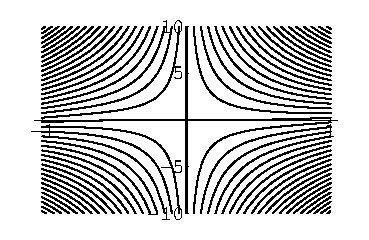
\includegraphics[width=0.4\textwidth]{ode/first_order/one_par}
    \end{center}
    \caption{The general solution for various values of the constant of
      integration.}
    \label{figure one param}
  \end{figure}

\end{Example}







%% y' - \frac{1}{x} y = x^\alpha.
\begin{Exercise}[mathematica/ode/first\_order/linear.nb]
  \label{exercise y - 1/x y = x alpha}
  Solve the differential equation
  \[
  y' - \frac{1}{x} y = x^\alpha, \quad x > 0.
  \]

  \hintsolution{y - 1/x y = x alpha}
\end{Exercise}







%%------------------------------------------------------------------------------
\subsection{Variation of Parameters.}
\index{variation of parameters!first order equation} 


We could also have found the particular solution with the method of 
variation of parameters. 
Although we can solve first order equations without this method, it will
become important in the study of higher order inhomogeneous equations.
We begin by assuming that the particular solution has the form 
$y_p = u(x) y_h(x)$ where $u(x)$ is an unknown function.  
We substitute this into the differential equation.
\begin{gather*}
  \frac{\dd}{\dd x} y_p + p(x) y_p = f(x) \\
  \frac{\dd}{\dd x} (u y_h) + p(x) u y_h = f(x) \\
  u' y_h + u (y_h' + p(x) y_h) = f(x) \\
  \intertext{Since $y_h$ is a homogeneous solution, $y_h' + p(x) y_h = 0$.}
  u' = \frac{f(x)}{y_h} \\
  u = \int \frac{f(x)}{y_h(x)}\,\dd x \\
  \intertext{Recall that the homogeneous solution is $y_h = \e^{-P(x)}$.}
  u = \int \e^{P(x)}f(x)\,\dd x
\end{gather*}
Thus the particular solution is
\[ 
y_p = \e^{-P(x)} \int \e^{P(x)}f(x)\,\dd x.
\]









%%=============================================================================
\section{Initial Conditions}
\index{initial conditions}




In physical problems involving first order differential equations, 
the solution satisfies both the differential equation and a constraint which 
we call the \textit{initial condition}.
Consider a first order linear differential equation subject to
the initial condition $y(x_0) = y_0$.  
The general solution is
\[ 
y = y_p + c y_h = \e^{-P(x)} \int \e^{P(x)} f(x) \,\dd x + c \e^{-P(x)}. 
\]
For the moment, we will assume that this problem is \textit{well-posed}.  
A problem is well-posed if there is a unique solution to the differential 
equation that satisfies the constraint(s).
Recall that $\int \e^{P(x)}f(x)\,\dd x$ denotes any integral of $\e^{P(x)} f(x)$.
For convenience, we choose $\int^x_{x_0} \e^{P(\xi)}f(\xi)\,\dd \xi$.  The initial
condition requires that
\[
y(x_0) = y_0 
= \e^{-P(x_0)}\int^{x_0}_{x_0} \e^{P(\xi)}f(\xi)\,\dd \xi + c \e^{-P(x_0)}
= c \e^{-P(x_0)}.
\]
Thus $c = y_0 \e^{P(x_0)}$. The solution subject to the initial condition is
\[
y = \e^{-P(x)}\int^x_{x_0} \e^{P(\xi)}f(\xi)\,\dd\xi + y_0 \e^{P(x_0)-P(x)}.
\]







\begin{Example}
  Consider the problem
  \[ 
  y' + (\cos x) y = x, \qquad y(0) = 2.
  \]
  From Result~\ref{first_order_inhom}, the solution subject to the initial 
  condition is
  \[ 
  \boxed{
    y = \e^{-\sin x} \int^x_0 \xi \e^{\sin \xi}\,\dd \xi + 2 \e^{-\sin x}.
    }
  \]
\end{Example}









%%-----------------------------------------------------------------------------
\subsection{Piecewise Continuous Coefficients and Inhomogeneities}


If the coefficient function $p(x)$ and the inhomogeneous term $f(x)$ in
the first order linear differential equation
\[ 
\frac{\dd y}{\dd x} + p(x) y = f(x) 
\]
are continuous, then the solution is continuous and has a continuous first 
derivative.   To see this, we note that the solution 
\[ 
y = \e^{-P(x)}\int \e^{P(x)}f(x)\,\dd x + c \e^{-P(x)}
\]
is continuous since the integral of a piecewise continuous function is
continuous.  The first derivative of the solution can be found directly
from the differential equation.
\[ 
y' = - p(x) y + f(x)
\]
Since $p(x)$, $y$, and $f(x)$ are continuous, $y'$ is continuous.

If $p(x)$ or $f(x)$ is only piecewise continuous, then the solution will be
continuous since the integral of a piecewise continuous function is continuous.
The first derivative of the solution will be piecewise continuous.






\begin{Example}
  Consider the problem
  \[ 
  y' - y = H(x-1), \qquad y(0) = 1,
  \]
  where $H(x)$ is the Heaviside function.
  \index{Heaviside function}
  \[ H(x) = 
  \begin{cases}
    1\ &\mathrm{for}\ x > 0, \\
    0\ &\mathrm{for}\ x < 0.
  \end{cases}
  \]
  To solve this problem, we divide it into two equations on separate domains.
  \begin{alignat*}{3}
    y_1' - y_1 &= 0, &\qquad y_1(0) &= 1, &\qquad \mathrm{for}\ x &< 1 \\
    y_2' - y_2 &= 1, &\qquad y_2(1) &= y_1(1), &\qquad \mathrm{for}\ x &> 1
  \end{alignat*}
  With the condition $y_2(1) = y_1(1)$ on the second equation, we demand that
  the solution be continuous.  The solution to the first equation is 
  $y = \e^x$.  The solution for the second equation is
  \[
  y = \e^x \int_1^x \e^{-\xi}\,\dd \xi + \e^1 \e^{x-1} = -1 + \e^{x-1} + \e^x.
  \]
  Thus the solution over the whole domain is
  \[ 
  \boxed{
    y = 
    \begin{cases}
      \e^x \ &\mathrm{for}\ x < 1,  \\
      (1+\e^{-1})\e^x-1 \ &\mathrm{for}\ x > 1.
    \end{cases}
    }
  \]
  The solution is graphed in Figure~\ref{heaviside}.

  \begin{figure}[tb!]
    \begin{center}
      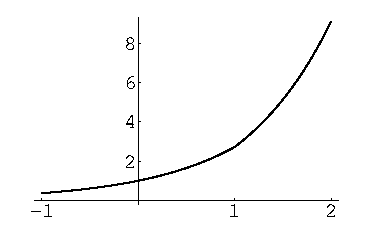
\includegraphics[width=0.4\textwidth]{ode/first_order/heavi}
    \end{center}
    \caption{The solution is continuous.}
    \label{heaviside}
  \end{figure}

\end{Example}
















\begin{Example}
  Consider the problem,
  \[ 
  y' + \sign(x) y = 0, \qquad y(1) = 1.
  \]
  Recall that 
  \[ 
  \sign x = 
  \begin{cases}
    -1 \quad &\mathrm{for}\ x < 0 \\
    0 \quad &\mathrm{for}\ x = 0 \\
    1 \quad &\mathrm{for}\ x > 0. 
  \end{cases}
  \]
  Since $\sign x$ is piecewise defined, we solve the two problems,
  \begin{alignat*}{3}
    y_+' + y_+ &= 0, &\qquad y_+(1) &= 1, &\qquad &\mathrm{for}\ x > 0 \\
    y_-' - y_- &= 0, &\qquad y_-(0) &= y_+(0), &\qquad &\mathrm{for}\ x < 0,
  \end{alignat*}
  and define the solution, $y$, to be
  \[ y(x) = 
  \begin{cases}
    y_+(x), \quad &\mathrm{for}\ x \geq 0, \\
    y_-(x), \quad &\mathrm{for}\ x \leq 0.
  \end{cases} \]
  The initial condition for $y_-$ demands that the solution be continuous.

  Solving the two problems for positive and negative $x$, we obtain
  \[ 
  y(x) = 
  \begin{cases}
    \e^{1-x},       \quad &\mathrm{for}\ x > 0, \\
    \e^{1+x}, \quad &\mathrm{for}\ x < 0.
  \end{cases} 
  \]
  This can be simplified to
  \[ 
  \boxed{
    y(x) = \e^{1 -|x|}.
    }
  \]
  This solution is graphed in Figure~\ref{figure epem}.

  \begin{figure}[tb!]
    \begin{center}
      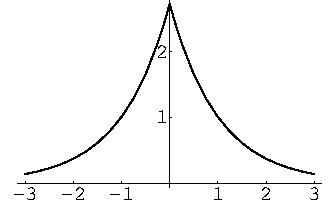
\includegraphics[width=0.4\textwidth]{ode/first_order/epem}
    \end{center}
    \caption{The solution.} 
    \label{figure epem}
  \end{figure}

\end{Example}





\begin{Result}
  \label{first_order_inhom}
  \textbf{Existence, Uniqueness Theorem.}
  Let $p(x)$ and $f(x)$ be piecewise continuous on the interval $[a,b]$
  and let $x_0 \in [a,b]$.  Consider the problem,
  \[ 
  \frac{\dd y}{\dd x} + p(x) y = f(x), \qquad y(x_0) = y_0.
  \]
  The general solution of the differential equation is
  \[ 
  y = \e^{-P(x)} \int \e^{P(x)}f(x)\,\dd x + c \e^{-P(x)}.
  \]
  The unique, continuous solution of the differential equation 
  subject to the initial condition is
  \[
  y = \e^{-P(x)}\int^x_{x_0} \e^{P(\xi)}f(\xi)\,\dd \xi + y_0 \e^{P(x_0)-P(x)},
  \]
  where $P(x) = \int p(x)\,\dd x$.
\end{Result}









%% \frac{\dd y}{\dd x} + x y = x^{2n+1}, \quad y(1) = 1, \quad n \in \mathbb{Z}
\begin{Exercise}[mathematica/ode/first\_order/exact.nb]
  \label{exercise dydx + x y = x 2n+1}
  Find the solutions of the following differential equations which satisfy the 
  given initial conditions:
  \begin{enumerate}
  \item
    $ \displaystyle
    \frac{\dd y}{\dd x} + x y = x^{2n+1}, \quad y(1) = 1, \quad n \in \mathbb{Z}
    $
  \item
    $ \displaystyle
    \frac{\dd y}{\dd x} - 2 x y = 1, \quad y(0) = 1
    $
  \end{enumerate}

  \hintsolution{dydx + x y = x 2n+1}
\end{Exercise}






%% \frac{\dd y}{\dd x} + \alpha y(x) = \beta \e^{-\lambda x}
\begin{Exercise}[mathematica/ode/first\_order/exact.nb]
  \label{exercise dydx + alpha y = beta e}
  Show that if $\alpha > 0$ and $\lambda > 0$, then for any real $\beta$, 
  every solution of 
  \[
  \frac{\dd y}{\dd x} + \alpha y(x) = \beta \e^{-\lambda x}
  \]
  satisfies $\lim_{x \to +\infty} y(x) = 0$.  (The case $\alpha = \lambda$
  requires special treatment.)  Find the solution for $\beta = \lambda = 1$
  which satisfies $y(0) = 1$.  Sketch this solution for $0 \leq x < \infty$
  for several values of $\alpha$.  In particular, show what happens when
  $\alpha \to 0$ and $\alpha \to \infty$.

  \hintsolution{dydx + alpha y = beta e}
\end{Exercise}










%%===========================================================================
\section{Well-Posed Problems}
\index{well-posed problems}
\index{ill-posed problems}





\begin{Example}
  Consider the problem,
  \[ 
  y' - \frac{1}{x} y = 0, \qquad y(0) = 1.
  \]
  The general solution is $y = c x$.  Applying the initial condition demands that
  $1 = c \cdot 0$, which cannot be satisfied.
  The general solution for various values of $c$ is plotted in 
  Figure~\ref{cx}.

  \begin{figure}[tb!]
    \begin{center}
      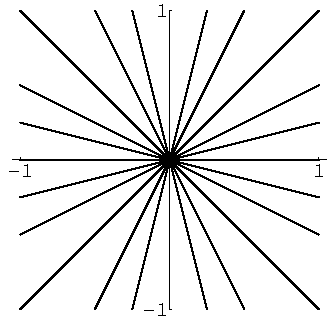
\includegraphics[width=0.3\textwidth]{ode/first_order/cx}
    \end{center}
    \caption{The general solution for various values of the constant
    of integration.}
    \label{cx}
  \end{figure}

\end{Example}








\begin{Example}
  Consider the problem
  \[ 
  y' - \frac{1}{x} y = -\frac{1}{x}, \qquad y(0) = 1.
  \]
  The general solution is 
  \[ 
  y = 1 + c x.
  \]
  The initial condition is satisfied for any value of $c$ so there are an 
  infinite number of solutions.
\end{Example}






\begin{Example}
  Consider the problem
  \[ 
  y' + \frac{1}{x} y = 0, \qquad y(0) = 1.
  \]
  The general solution is $y = \frac{c}{x}$.  
  Depending on whether $c$ is nonzero, the solution is either singular or zero 
  at the origin and cannot satisfy the initial condition.
\end{Example}




The above problems in which there were either no solutions or an infinite
number of solutions are said to be \textit{ill-posed}.  
If there is a unique solution that satisfies the initial condition, 
the problem is said to be \textit{well-posed}.  We should have suspected that
we would run into trouble in the above examples as the initial condition 
was given at a singularity of the coefficient function, $p(x) = 1/x$.

Consider the problem,
\[
y' + p(x) y = f(x), \qquad y(x_0) = y_0.
\]
We assume that $f(x)$ bounded in a neighborhood of $x = x_0$.
The differential equation has the general solution,
\[ 
y = \e^{-P(x)} \int \e^{P(x)}f(x)\,\dd x + c \e^{-P(x)}.
\]
If the homogeneous solution, $\e^{-P(x)}$, is nonzero and finite at $x = x_0$, 
then there is a unique value of $c$ for which the initial condition is 
satisfied.   If the homogeneous solution vanishes at $x = x_0$ then either
the initial condition cannot be satisfied or the initial condition is
satisfied for all values of $c$.   The homogeneous solution can vanish
or be infinite only if $P(x) \to \pm \infty$ as $x \to x_0$.   This can
occur only if the coefficient function, $p(x)$, is unbounded at that point.













\begin{Result}
  If the initial condition is given where the homogeneous solution to a first 
  order, linear differential equation is zero or infinite then the problem 
  may be ill-posed.  This may occur only if the coefficient function,
  $p(x)$, is unbounded at that point.
\end{Result}









%%=============================================================================
\section{Equations in the Complex Plane}
\index{complex plane!first order differential equations}




%%----------------------------------------------------------------------------
\subsection{Ordinary Points}
\index{ordinary points!first order differential equations}




Consider the first order homogeneous equation
\[ 
\frac{\dd w}{\dd z} + p(z) w = 0, 
\]
where $p(z)$, a function of a complex variable, is analytic in some domain $D$.
The integrating factor,
\[ 
I(z) = \exp \left( \int p(z) \,\dd z \right),
\]
is an analytic function in that domain.  As with the case of real variables, 
multiplying by the integrating factor and integrating yields the solution,
\[
w(z) = c \exp\left(-\int p(z)\,\dd z \right). 
\] 
We see that the solution is analytic in $D$. 





\begin{Example} 
  It does not make sense to pose the equation
  \[ \frac{\dd w}{\dd z} + |z| w = 0. \]
  For the solution to exist, $w$ and hence $w'(z)$ must be analytic.  
  Since $p(z) = |z|$ is not analytic anywhere in the complex plane, the
  equation has no solution.
\end{Example}




Any point at which $p(z)$ is analytic is called an \textit{ordinary point} 
of the differential equation.
Since the solution is analytic we can expand it in a Taylor series about
an ordinary point. The radius of convergence of the series will be at least the 
distance to the nearest singularity of $p(z)$ in the complex plane.




\begin{Example} 
  \label{ssrp_expand_solution}
  Consider the equation
  \[ 
  \frac{\dd w}{\dd z} - \frac{1}{1-z} w = 0.
  \]
  The general solution is $w = \frac{c}{1-z}.$  Expanding this solution 
  about the origin,
  \[ 
  w = \frac{c}{1-z} = c\sum_{n=0}^\infty z^n.
  \]
  The radius of convergence of the series is,
  \[
  R = \lim_{n \to \infty} \left|\frac{a_n}{a_{n+1}} \right| = 1,
  \]
  which is the distance from the origin to the nearest singularity of 
  $p(z) = \frac{1}{1-z}$.
\end{Example}




We do not need to solve the differential equation to find the Taylor series
expansion of the homogeneous solution.  
\index{Taylor series!first order differential equations}
We could substitute a general Taylor series expansion into
the differential equation and solve for the coefficients.  Since we can 
always solve first order equations, this method is of limited usefulness.
However, when we consider higher order equations in which we cannot 
solve the equations exactly, this will become an important method.




\begin{Example}
  Again consider the equation
  \[ 
  \frac{\dd w}{\dd z} - \frac{1}{1-z} w = 0.
  \]
  Since we know that the solution has a Taylor series expansion about $z=0$,
  we substitute $w = \sum_{n=0}^\infty a_n z^n$ into the differential equation.
  \begin{gather*}
    (1-z) \frac{\dd}{\dd z} \sum_{n=0}^\infty a_n z^n 
    - \sum_{n=0}^\infty a_n z^n = 0 \\
    \sum_{n=1}^\infty n a_n z^{n-1} - \sum_{n=1}^\infty n a_n z^n 
    - \sum_{n=0}^\infty a_n z^n = 0 \\
    \sum_{n=0}^\infty (n+1) a_{n+1} z^n - \sum_{n=0}^\infty n a_n z^n 
    - \sum_{n=0}^\infty a_n z^n = 0 \\
    \sum_{n=0}^\infty \left((n+1) a_{n+1} - (n+1) a_n \right) z^n = 0.
  \end{gather*}
  Now we equate powers of $z$ to zero.  For $z^n$, the equation is 
  $(n+1) a_{n+1} - (n+1) a_n = 0$, or $a_{n+1} = a_n$.  Thus we have that
  $a_n = a_0$ for all $n \geq 1$.  The solution is then
  \[ 
  \boxed{ 
    w = a_0 \sum_{n=0}^\infty z^n, 
    } 
  \]
  which is the result we obtained by expanding the solution in 
  Example~\ref{ssrp_expand_solution}.
\end{Example}




\begin{Result}
  Consider the equation
  \[ 
  \frac{\dd w}{\dd z} + p(z) w = 0. 
  \]
  If $p(z)$ is analytic at $z = z_0$ then $z_0$ is called an ordinary point
  of the differential equation.  The Taylor series expansion of the solution
  can be found by substituting $w = \sum_{n=0}^\infty a_n (z-z_0)^n$ into the 
  equation and equating powers of $(z-z_0)$.  The radius of convergence of the
  series is at least the distance to the nearest singularity of $p(z)$ in 
  the complex plane.
\end{Result}






%% Taylor series about origin
\begin{Exercise} 
  \label{exercise dwdz + 1 1-z w}
  Find the Taylor series expansion about the origin of the solution to
  \[
  \frac{\dd w}{\dd z} + \frac{1}{1-z} w = 0
  \]
  with the substitution $w = \sum_{n=0}^\infty a_n z^n$.  What is the 
  radius of convergence of the series?  What is the distance to the nearest
  singularity of $\frac{1}{1-z}$?

  \hintsolution{dwdz + 1 1-z w}
\end{Exercise}











%%----------------------------------------------------------------------------
\subsection{Regular Singular Points}
\index{regular singular points!first order differential equations}



If the coefficient function $p(z)$ has a simple pole at $z = z_0$ then $z_0$ 
is a \textit{regular singular point} of the first order differential equation.





\begin{Example}
  Consider the equation
  \[
  \frac{\dd w}{\dd z} + \frac{\alpha}{z} w = 0, \qquad \alpha \neq 0.
  \]
  This equation has a regular singular point at $z = 0$.
  The solution is $w = c z^{-\alpha}$.  Depending on the value of $\alpha$, the
  solution can have three different kinds of behavior.

  \begin{description}
    %%
  \item{$\boldsymbol{\alpha}$ \textbf{is a negative integer.}}
    The solution is analytic in the finite complex plane.
    %%
  \item{$\boldsymbol{\alpha}$ \textbf{is a positive integer}}
    The solution has a pole at the origin.  
    $w$ is analytic in the annulus, $0<|z|$.
    %%
  \item{$\boldsymbol{\alpha}$ \textbf{is not an integer.}}
    $w$ has a branch point at $z=0$.
    The solution is analytic in the cut annulus $0 < |z| < \infty $, 
    $\theta_0 < \arg z < \theta_0 + 2 \pi$.
  \end{description}
\end{Example}




Consider the differential equation
\[ 
\frac{\dd w}{\dd z} + p(z) w = 0, 
\]
where $p(z)$ has a simple pole at the origin and is analytic in the annulus, 
$0 < |z| < r$, for some positive $r$.  Recall that the solution is
\begin{align*}
  w       &= c \exp \left(- \int p(z)\,\dd z \right) \\
  &= c \exp \left(- \int \frac{b_0}{z} + p(z) - \frac{b_0}{z} \,\dd z 
  \right) \\
  &= c \exp \left( - b_0 \log z - \int \frac{z p(z) - b_0}{z} \,\dd z 
  \right) \\
  &= c z^{-b_0} \exp \left(  - \int \frac{z p(z) - b_0}{z} \,\dd z \right)
\end{align*}

The exponential factor has a removable singularity at $z = 0$ and is analytic 
in $|z| < r$.  We consider the following cases for the $z^{-b_0}$ factor:
\begin{description}
  %%
\item{$\mathbf{b_0}$ \textbf{is a negative integer.}}
  Since $z^{-b_0}$ is analytic at the origin, the solution to the differential
  equation is analytic in the circle $|z| < r$.
  %%
\item{$\mathbf{b_0}$ \textbf{is a positive integer.}}
  The solution has a pole of order $-b_0$ at the origin and is analytic
  in the annulus $0 < |z| < r$.
  %%
\item{$\mathbf{b_0}$ \textbf{is not an integer.}}
  The solution has a branch point at the origin and thus is not single-valued.
  The solution is analytic in the cut annulus $0 < |z| < r$, 
  $\theta_0 < \arg z < \theta_0 + 2\pi$.
\end{description}

Since the exponential factor has a convergent Taylor series in $|z|<r$,
the solution can be expanded in a series of the form
\index{Laurent series!first order differential equation}
\[ 
w = z^{-b_0} \sum_{n=0}^\infty a_n z^n, 
\quad \mathrm{where}\ a_0 \neq 0\ 
\mathrm{and}\ b_0 = \lim_{z \to 0} z\,p(z).
\]
In the case of a regular singular point at $z = z_0$, the series is
\[ 
w = (z - z_0)^{-b_0} \sum_{n=0}^\infty a_n (z-z_0)^n, 
\quad \mathrm{where}\ a_0 \neq 0\ 
\mathrm{and}\ b_0 = \lim_{z \to z_0}(z-z_0)\,p(z).
\]


Series of this form are known as \textit{Frobenius series}. 
\index{Frobenius series!first order differential equation}
Since we can write the solution as
\[ 
w = c (z-z_0)^{-b_0} \exp \left(- \int 
  \left( p(z) - \frac{b_0}{z-z_0} \right) \,\dd z \right),
\]
we see that the Frobenius expansion of the solution will have a radius of 
convergence at least the distance to the nearest singularity of $p(z)$.




\begin{Result}
  Consider the equation,
  \[ 
  \frac{\dd w}{\dd z} + p(z) w = 0,
  \]
  where $p(z)$ has a simple pole at $z=z_0$, $p(z)$ is analytic in some
  annulus, $0 < |z-z_0| < r$, and $\lim_{z \to z_0} (z-z_0) p(z) = \beta$.
  The solution to the differential equation has a Frobenius series expansion
  of the form
  \[ 
  w = (z-z_0)^{-\beta} \sum_{n=0}^\infty a_n (z-z_0)^n, \qquad a_0 \neq 0.
  \]
  The radius of convergence of the expansion will be at least the 
  distance to the nearest singularity of $p(z)$.
\end{Result}








\begin{Example}
  We will find the first two nonzero terms in the series solution about $z = 0$ 
  of the differential equation,
  \[ 
  \frac{\dd w}{\dd z} + \frac{1}{\sin z} w = 0.
  \]
  First we note that the coefficient function has a simple pole at $z = 0$ and
  \[ 
  \lim_{z \to 0} \frac{z}{\sin z} = \lim_{z \to 0} \frac{1}{\cos z} = 1.
  \]
  Thus we look for a series solution of the form
  \[ 
  w = z^{-1} \sum_{n=0}^\infty a_n z^n, \qquad a_0 \neq 0.
  \]
  The nearest singularities of $1 / \sin z$ in the complex plane are at 
  $z = \pm \pi$.  Thus the radius of convergence of the series will
  be at least $\pi$.

  Substituting the first three terms of the expansion into the differential 
  equation,
  \begin{gather*}
    \frac{\dd}{\dd z}(a_0 z^{-1} + a_1 + a_2 z) 
    + \frac{1}{\sin z} (a_0 z^{-1} + a_1 + a_2 z) = O(z). \\
    \intertext{Recall that the Taylor expansion of $\sin z$ is 
      $\sin z = z - \frac{1}{6}z^3 + O(z^5)$.}
    \left(z - \frac{z^3}{6} + O(z^5)\right)
    (-a_0 z^{-2} + a_2) + (a_0 z^{-1} + a_1 + a_2 z) = O(z^2)\\
    -a_0 z^{-1} + \left(a_2 + \frac{a_0}{6}\right)z + a_0 z^{-1} + a_1 + a_2 z 
    = O(z^2) \\
    a_1 + \left(2a_2 + \frac{a_0}{6}\right) z = O(z^2)
  \end{gather*}
  $a_0$ is arbitrary.  Equating powers of $z$,
  \begin{align*}
    &z^0: \qquad a_1 = 0. \\
    &z^1: \qquad 2a_2 + \frac{a_0}{6} = 0.
  \end{align*}
  Thus the solution has the expansion,
  \[
  \boxed{
    w = a_0 \left(z^{-1} - \frac{z}{12} \right) + O(z^2).
    }
  \]
  In Figure~\ref{figure foode oosc} the exact solution is plotted in a solid 
  line and the two term approximation is plotted in a dashed line.  The two
  term approximation is very good near the point $x = 0$.

  \begin{figure}[tb!]
    \begin{center}
      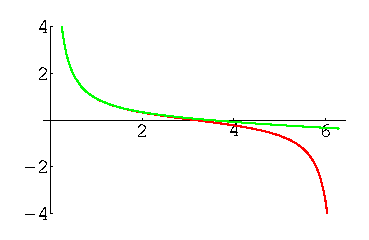
\includegraphics[width=0.4\textwidth]{ode/first_order/oosc}
    \end{center}
    \caption{Plot of the exact solution and the two term approximation.}
    \label{figure foode oosc}
  \end{figure}

\end{Example}














\begin{Example}
  Find the first two nonzero terms in the series expansion about $z=0$ 
  of the solution to
  \[
  w' - i \frac{\cos z}{z} w = 0.
  \]
  Since $\frac{\cos z}{z}$ has a simple pole at $z=0$ and 
  $\lim_{z \to 0} -i \cos z = -i$
  we see that the Frobenius series will have the form
  \[ 
  w = z^i \sum_{n=0}^\infty a_n z^n, \qquad a_0 \neq 0.
  \]
  Recall that $\cos z$ has the Taylor expansion 
  $\sum_{n=0}^\infty \frac{(-1)^n z^{2n}}{(2n)!}$.  
  Substituting the Frobenius expansion into the differential equation yields
  \begin{gather*}
    z \left( i z^{i-1} \sum_{n=0}^\infty a_n z^n 
      + z^i \sum_{n=0}^\infty n a_n z^{n-1} \right)
    - i \left(\sum_{n=0}^\infty \frac{(-1)^n z^{2n}}{(2n)!}\right)
    \left( z^i \sum_{n=0}^\infty a_n z^n\right) = 0 \\
    \sum_{n=0}^\infty(n+i)a_n z^n 
    -i  \left(\sum_{n=0}^\infty \frac{(-1)^n z^{2n}}{(2n)!}\right)
    \left(\sum_{n=0}^\infty a_n z^n\right) = 0. 
  \end{gather*}
  Equating powers of $z$,
  \begin{alignat*}{2}
    &z^0:   &\quad  &i a_0 -i a_0 = 0 \qquad \to a_0\ \mathrm{is arbitrary} \\
    &z^1:   &\quad  &(1+i)a_1 - i a_1 = 0 \qquad \to a_1 = 0 \\
    &z^2:   &\quad  &(2+i)a_2 - i a_2 + \frac{i}{2} a_0 = 0 
    \qquad \to a_2 = -\frac{i}{4}a_0.
  \end{alignat*}
  Thus the solution is
  \[ 
  \boxed{
    w = a_0 z^i \left(1 -\frac{i}{4}z^2 + O(z^3) \right).
    }
  \]
\end{Example}











%%----------------------------------------------------------------------------
\subsection{Irregular Singular Points}
\index{irregular singular points!first order differential equations}


If a point is not an ordinary point or a regular singular point then it 
is called an \textit{irregular singular point}. The following equations have
irregular singular points at the origin.
\begin{itemize}
\item $w' + \sqrt{z} w = 0$ 
\item $w' - z^{-2} w = 0$ 
\item $w' + \exp(1/z) w = 0$
\end{itemize}





\begin{Example}
  Consider the differential equation
  \[ 
  \frac{\dd w}{\dd z}  + \alpha z^\beta w = 0, 
  \qquad \alpha \neq 0, \quad \beta \neq -1, 0, 1, 2, \ldots
  \]
  This equation has an irregular singular point at the origin.
  Solving this equation,
  \begin{gather*}
    \frac{\dd}{\dd z} \left(\exp\left(\int \alpha z^\beta\,\dd z \right) w \right)=0\\
    \boxed{ 
      w = c \exp \left(- \frac{\alpha}{\beta+1} z^{\beta+1}\right) = 
      c \sum_{n = 0}^\infty \frac{(-1)^n}{n!} \left( \frac{\alpha}{\beta+1} \right)^n
      z^{(\beta+1)n}. 
      }
  \end{gather*}
  If $\beta$ is not an integer, then the solution has a branch point at the
  origin.  If $\beta$ is an integer, $\beta < -1$, then the solution
  has an essential singularity at the origin.
  The solution cannot be expanded in a Frobenius series,
  $w = z^\lambda \sum_{n=0}^\infty a_n z^n$.  
\end{Example}




Although we will not show it, this result holds for any irregular singular
point of the differential equation.  We cannot approximate 
the solution near an irregular singular point using a Frobenius expansion.

Now would be a good time to summarize what we have discovered about
solutions of first order differential equations in the complex plane.


\begin{Result}
  Consider the first order differential equation
  \[ 
  \frac{\dd w}{\dd z} + p(z) w = 0.
  \]
  \begin{description}
    %%
  \item{\textbf{Ordinary Points}}  If $p(z)$ is analytic at $z=z_0$ then
    $z_0$ is an ordinary point of the differential equation.  The solution can be 
    expanded in the Taylor series $w = \sum_{n=0}^\infty a_n (z-z_0)^n$.  The
    radius of convergence of the series is at least the distance to the nearest
    singularity of $p(z)$ in the complex plane.
    %%
  \item{\textbf{Regular Singular Points}} If $p(z)$ has a simple pole at 
    $z = z_0$ and is analytic in some annulus $0 < |z-z_0| < r$ then $z_0$
    is a regular singular point of the differential equation.  The solution
    at $z_0$ will either be analytic, have a pole, or have a branch point.
    The solution can be expanded in the Frobenius series
    $w = (z-z_0)^{-\beta} \sum_{n=0}^\infty a_n (z-z_0)^n$ where $a_0 \neq 0$
    and $\beta = \lim_{z \to z_0} (z-z_0) p(z)$.  The radius of convergence of the
    Frobenius series will be at least the distance to the nearest singularity
    of $p(z)$.
    %%
  \item{\textbf{Irregular Singular Points}} If the point $z=z_0$ is not
    an ordinary point or a regular singular point, then it is an irregular singular
    point of the differential equation.  The solution cannot be expanded in a 
    Frobenius series about that point.
  \end{description}
\end{Result}








%%----------------------------------------------------------------------------
\subsection{The Point at Infinity}
\label{fode:section:ecp:sub:pi}
\index{infinity!first order differential equation}


Now we consider the behavior of first order linear differential equations
at the point at infinity.  Recall from complex variables that the 
complex plane together with the point at infinity is called the
extended complex plane.  To study the behavior of a function $f(z)$ at 
infinity, we make the transformation $z = \frac{1}{\zeta}$ and study the 
behavior of $f(1/\zeta)$ at $\zeta=0$.


\begin{Example}
  Let's examine the behavior of $\sin z$ at infinity.  We make the substitution
  $z = 1/\zeta$ and find the Laurent expansion about $\zeta=0$.
  \[
  \sin(1/\zeta) = \sum_{n=0}^\infty \frac{(-1)^n}{(2n+1)! \, \zeta^{(2n+1)}}
  \]
  Since $\sin(1/\zeta)$ has an essential singularity at $\zeta=0$,
  $\sin z$ has an essential singularity at infinity.
\end{Example}




We use the same approach if we want to examine the behavior at infinity of a 
differential equation.  Starting with the first order differential equation,
\[ 
\frac{\dd w}{\dd z} + p(z) w = 0,
\]
we make the substitution
\[ 
z = \frac{1}{\zeta}, \qquad \frac{\dd}{\dd z} = -\zeta^2 \frac{\dd}{\dd \zeta}, 
\qquad w(z) = u(\zeta) 
\]
to obtain
\begin{gather*}
  -\zeta^2 \frac{\dd u}{\dd \zeta} + p(1/\zeta) u = 0 \\
  \frac{\dd u}{\dd \zeta} - \frac{p(1/\zeta)}{\zeta^2} u = 0.
\end{gather*}




\begin{Result}
  The behavior at infinity of
  \[ 
  \frac{\dd w}{\dd z} + p(z) w = 0
  \]
  is the same as the behavior at $\zeta=0$ of
  \[
  \frac{\dd u}{\dd \zeta} - \frac{p(1/\zeta)}{\zeta^2} u = 0.
  \]
\end{Result}






\begin{Example}
  We classify the singular points of the equation
  \[
  \frac{\dd w}{\dd z} + \frac{1}{z^2 + 9} w = 0.
  \]
  We factor the denominator of the fraction 
  to see that $z = \imath 3$ and $z = - \imath 3$ are regular singular points.  
  \[
  \frac{\dd w}{\dd z} + \frac{1}{(z - \imath 3)(z + \imath 3)} w = 0
  \]
  We make the transformation $z = 1 / \zeta$ to examine the point at infinity.
  \begin{gather*}
    \frac{\dd u}{\dd \zeta} - \frac{1}{\zeta^2}\frac{1}{(1/\zeta)^2+9} u = 0 
    \\
    \frac{\dd u}{\dd \zeta} - \frac{1}{9 \zeta^2 + 1} u = 0 
  \end{gather*}
  Since the equation for $u$ has a ordinary point at $\zeta = 0$, 
  $z = \infty$ is a ordinary point of the equation for $w$.
\end{Example}






















\raggedbottom
%%============================================================================
\exercises{
\pagebreak
\flushbottom
\section{Additional Exercises}





%%-----------------------------------------------------------------------------
\begin{large}
  \noindent
  \textbf{Exact Equations}
\end{large}





\begin{Exercise}[mathematica/ode/first\_order/exact.nb]
  \label{exercise dydx=xxyyx}
  Find the general solution $y=y(x)$ of the equations
  \begin{enumerate}
    \centering
  \item
    $\displaystyle \frac{\dd y}{\dd x} = \frac{ x^2 + x y + y^2 }{ x^2 }$,
  \item
    $\displaystyle (4y-3x) \,\dd x + (y-2x) \,\dd y = 0$.
  \end{enumerate}

  \hintsolution{dydx=xxyyx}
\end{Exercise}









\begin{Exercise}[mathematica/ode/first\_order/exact.nb]
  \label{exercise dydx=axbybxcy}
  Determine whether or not the following equations can be made exact.
  If so find the corresponding general solution.
  \begin{enumerate}
    \centering
  \item
    $\displaystyle (3x^2-2xy+2) \,\dd x+(6y^2-x^2+3) \,\dd y = 0$
  \item
    $\displaystyle \frac{\dd y}{\dd x}=-\frac{ax+by}{bx+cy}$
  \end{enumerate}

  \hintsolution{dydx=axbybxcy}
\end{Exercise}





\begin{Exercise}[mathematica/ode/first\_order/exact.nb]
  \label{exercise dydx = 1-2x y2}
  Find the solutions of the following differential equations
  which satisfy the given initial condition. In each case determine
  the interval in which the solution is defined.
  \begin{enumerate}
    \centering
  \item
    $\displaystyle \frac{\dd y}{\dd x} = (1-2x) y^2, \quad y(0) = -1/6$.
  \item
    $\displaystyle x \,\dd x + y \e^{-x} \,\dd y = 0, \quad y(0) = 1$.
  \end{enumerate}

  \hintsolution{dydx = 1-2x y2}
\end{Exercise}








%% (4 y - x) y' - (9 x^2 + y - 1) = 0.
\begin{Exercise}
  \label{exercise 4yxy9x2y10}
  Are the following equations exact?  If so, solve them.
  \begin{enumerate}
  \item
    $ \displaystyle
    (4 y - x) y' - (9 x^2 + y - 1) = 0
    $
  \item
    $ \displaystyle
    (2 x - 2 y) y' + (2 x + 4 y) = 0.
    $
  \end{enumerate}

  \hintsolution{4yxy9x2y10}
\end{Exercise}










%% y^2 \sin t + y f(t) \frac{\dd y}{\dd t} = 0
\begin{Exercise}[mathematica/ode/first\_order/exact.nb]
  \label{exercise y2 sin t + y f dydt}
  Find all functions $f(t)$ such that the differential equation
  \begin{equation}
    \label{eqn_y2_sint}
    y^2 \sin t + y f(t) \frac{\dd y}{\dd t} = 0
  \end{equation}
  is exact.  Solve the differential equation for these $f(t)$.

  \hintsolution{y2 sin t + y f dydt}
\end{Exercise}






%%-----------------------------------------------------------------------------
\begin{large}
  \noindent
  \textbf{The First Order, Linear Differential Equation}
\end{large}



%% y' + \frac{y}{\sin x} = 0. 
\begin{Exercise}[mathematica/ode/first\_order/linear.nb]
  \label{exercise y + y / sin x}
  Solve the differential equation
  \[ 
  y' + \frac{y}{\sin x} = 0. 
  \]

  \hintsolution{y + y / sin x}
\end{Exercise}




%%-----------------------------------------------------------------------------
\begin{large}
  \noindent
  \textbf{Initial Conditions}
\end{large}







%%-----------------------------------------------------------------------------
\begin{large}
  \noindent
  \textbf{Well-Posed Problems}
\end{large}





%% t \frac{\dd y}{\dd t} + A y = 1 + t^2
\begin{Exercise}
  \label{exercise t dydt + A y}
  Find the solutions of
  \[
  t \frac{\dd y}{\dd t} + A y = 1 + t^2, \quad t > 0
  \]
  which are bounded at $t = 0$.  Consider all (real) values of $A$.

  \hintsolution{t dydt + A y}
\end{Exercise}



%%-----------------------------------------------------------------------------
\begin{large}
  \noindent
  \textbf{Equations in the Complex Plane}
\end{large}




%% Classify the singular points of the following first order differential
\begin{Exercise} 
  \label{exercise dwdz + sin z z w}
  Classify the singular points of the following first order differential
  equations, (include the point at infinity).
  \begin{enumerate}
  \item $w' + \frac{\sin z}{z} w = 0$
  \item $w' + \frac{1}{z-3} w = 0$
  \item $w' + z^{1/2} w = 0$
  \end{enumerate}

  \hintsolution{dwdz + sin z z w}
\end{Exercise}







%% Expand irregular singular point in a Frobenius series.
\begin{Exercise} 
  \label{exercise dwdz z-2 w}
  Consider the equation
  \[ 
  w' + z^{-2}w = 0.
  \]
  The point $z = 0$ is an irregular singular point of the differential
  equation.  Thus we know that we cannot expand the solution about
  $z=0$ in a Frobenius series.  Try substituting the series solution
  \[
  w = z^\lambda \sum_{n=0}^\infty a_n z^n, \qquad a_0 \neq 0
  \]
  into the differential equation anyway.  What happens?

  \hintsolution{dwdz z-2 w}
\end{Exercise}



































\raggedbottom
}
%%============================================================================
\pagebreak
\flushbottom
\section{Hints}



%% Solve first order equations by inspection.
\begin{Hint}
  \label{hint gygyf}
  $\phantom{a}$

  \begin{enumerate}
    %%
  \item $\frac{\dd}{\dd x} \ln |u| = \frac{1}{u}$
    %%
  \item $\frac{\dd}{\dd x} u^c = u^{c-1} u'$
  \end{enumerate}
\end{Hint}






%% \mu(x,y) = \frac{1}{x M(x,y) + y N(x,y)}
\begin{Hint}
  \label{hint integrating factor homogeneous}
  %% CONTINUE
\end{Hint}





%% $d y / d t = f(y / t)$.
\begin{Hint}
  \label{hint dydt = f(y/t)}
  The equation is homogeneous.  Make the change of variables $u = y / t$.
\end{Hint}




%% y' - \frac{1}{x} y = x^\alpha.
\begin{Hint}
  \label{hint y - 1/x y = x alpha}
  Make sure you consider the case $\alpha = 0$.
\end{Hint}




%% \frac{\dd y}{\dd x} + x y = x^{2n+1}, \quad y(1) = 1, \quad n \in \mathbb{Z}
\begin{Hint}
  \label{hint dydx + x y = x 2n+1}
  %% CONTINUE
\end{Hint}



%% \frac{\dd y}{\dd x} + \alpha y(x) = \beta \e^{-\lambda x}
\begin{Hint}
  \label{hint dydx + alpha y = beta e}
  %% CONTINUE
\end{Hint}





%% Taylor series about origin
\begin{Hint} 
  \label{hint dwdz + 1 1-z w}
  The radius of convergence of the series and the distance to the nearest 
  singularity of $\frac{1}{1-z}$ are not the same.
\end{Hint}








\hints{
%%-----------------------------------------------------------------------------
\begin{large}
  \noindent
  \textbf{Exact Equations}
\end{large}



\begin{Hint}
  \label{hint dydx=xxyyx}
  \begin{enumerate}
  \item
  \item
  \end{enumerate}
\end{Hint}




\begin{Hint}
  \label{hint dydx=axbybxcy}
  \begin{enumerate}
  \item
    The equation is exact.  Determine the primitive $u$ by solving the equations
    $u_x = P$, $u_y = Q$.
  \item
    The equation can be made exact.
  \end{enumerate}
\end{Hint}






\begin{Hint}
  \label{hint dydx = 1-2x y2}
  \begin{enumerate}
  \item
    This equation is separable.  Integrate to get the general solution.
    Apply the initial condition to determine the constant of integration.
  \item
    Ditto.  You will have to numerically solve an equation to determine where
    the solution is defined.
  \end{enumerate}
\end{Hint}






%% (4 y - x) y' - (9 x^2 + y - 1) = 0.
\begin{Hint}
  \label{hint 4yxy9x2y10}
  %% CONTINUE
\end{Hint}










%% y^2 \sin t + y f(t) \frac{\dd y}{\dd t} = 0
\begin{Hint}
  \label{hint y2 sin t + y f dydt}
  %% CONTINUE
\end{Hint}





%%-----------------------------------------------------------------------------
\begin{large}
  \noindent
  \textbf{The First Order, Linear Differential Equation}
\end{large}



%% y' + \frac{y}{\sin x} = 0. 
\begin{Hint}
  \label{hint y + y / sin x}
  Look in the appendix for the integral of $\csc x$.
\end{Hint}




%%-----------------------------------------------------------------------------
\begin{large}
  \noindent
  \textbf{Initial Conditions}
\end{large}





%%-----------------------------------------------------------------------------
\begin{large}
  \noindent
  \textbf{Well-Posed Problems}
\end{large}




%% t \frac{\dd y}{\dd t} + A y = 1 + t^2
\begin{Hint}
  \label{hint t dydt + A y}
  %% CONTINUE
\end{Hint}







%%-----------------------------------------------------------------------------
\begin{large}
  \noindent
  \textbf{Equations in the Complex Plane}
\end{large}



%% Classify the singular points of the following first order differential
\begin{Hint}
  \label{hint dwdz + sin z z w}
  %% CONTINUE
\end{Hint}



%% Expand irregular singular point in a Frobenius series.
\begin{Hint}
  \label{hint dwdz z-2 w}
  Try to find the value of $\lambda$ by substituting the series into the 
  differential equation and equating powers of $z$.
\end{Hint}


















\raggedbottom
}
%%============================================================================
\pagebreak
\flushbottom
\section{Solutions}



%% Solve first order equations by inspection.
\begin{Solution}
  \label{solution gygyf}
  $\phantom{a}$

  \begin{enumerate}
    %%
  \item
    \begin{gather*}
      \frac{y'(x)}{y(x)} = f(x) 
      \\
      \frac{\dd}{\dd x} \ln |y(x)| = f(x) 
      \\
      \ln |y(x)| = \int f(x) \,\dd x + c 
      \\
      y(x) = \pm \e^{\int f(x) \,\dd x + c} 
      \\
      \boxed{
        y(x) = c \e^{\int f(x) \,\dd x} 
        }
    \end{gather*}
    %%
  \item
    \begin{gather*}
      y^\alpha(x) y'(x) = f(x) 
      \\
      \frac{ y^{\alpha+1}(x) }{ \alpha + 1 } = \int f(x)\,\dd x + c 
      \\
      \boxed{
        y(x) = \left( (\alpha+1) \int f(x)\,\dd x + a \right)^{1/(\alpha+1)}
        }
    \end{gather*}
    %%
  \item
    \begin{gather*} 
      \frac{y'}{\cos x} + y \frac{\tan x}{\cos x} = \cos x 
      \\
      \frac{\dd}{\dd x} \left( \frac{y}{\cos x} \right) = \cos x 
      \\
      \frac{y}{\cos x} =  \sin x + c 
      \\
      \boxed{ 
        y(x) = \sin x \cos x + c \cos x
        } 
    \end{gather*}
  \end{enumerate}
\end{Solution}





%% \mu(x,y) = \frac{1}{x M(x,y) + y N(x,y)}
\begin{Solution}
  \label{solution integrating factor homogeneous}
  We consider the homogeneous equation,
  \[
  P(x,y) + Q(x,y) \frac{\dd y}{\dd x} = 0.
  \]
  That is, both $P$ and $Q$ are homogeneous of degree $n$.  We hypothesize 
  that multiplying by
  \[
  \mu(x,y) = \frac{1}{x P(x,y) + y Q(x,y)}
  \]
  will make the equation exact.  To prove this we use the result that 
  \[
  M(x,y) + N(x,y) \frac{\dd y}{\dd x} = 0
  \]
  is exact if and only if $M_y = N_x$.
  \begin{align*}
    M_y &= \frac{\partial}{\partial y} \left[ \frac{ P }{ x P + y Q } \right] 
    \\
    &= \frac{ P_y (x P + y Q) - P (x P_y + Q + y Q_y) }{ (x P + y Q)^2 } 
  \end{align*}
  \begin{align*}
    N_x &= \frac{\partial}{\partial x} \left[ \frac{ Q }{ x P + y Q } \right] 
    \\
    &= \frac{ Q_x (x P + y Q) - Q (P + x P_x + y Q_x) }{ (x P + y Q)^2 }
  \end{align*}
  \begin{gather*}
    M_y = N_x
    \\
    P_y (x P + y Q) - P (x P_y + Q + y Q_y)
    = Q_x (x P + y Q) - Q (P + x P_x + y Q_x) 
    \\
    y P_y Q - y P Q_y = x P Q_x - x P_x Q  
    \\
    x P_x Q + y P_y Q = x P Q_x + y P Q_y 
    \\
    (x P_x + y P_y) Q = P (x Q_x + y Q_y)
    \\
    \intertext{With Euler's theorem, this reduces to an identity.}
    n P Q = P n Q
  \end{gather*}
  Thus the equation is exact.  $\mu(x,y)$ is an integrating factor for 
  the homogeneous equation.
\end{Solution}







%% $d y / d t = f(y / t)$.
\begin{Solution}
  \label{solution dydt = f(y/t)}
  We note that this is a homogeneous differential equation.  The coefficient
  of $\dd y / \dd t$ and the inhomogeneity are homogeneous of degree zero.
  \[
  \frac{\dd y}{\dd t} 
  = 2 \left( \frac{y}{t} \right) + \left( \frac{y}{t} \right)^2.
  \]
  We make the change of variables $u = y / t$ to obtain a separable equation.
  \begin{gather*}
    t u' + u = 2 u + u^2
    \\
    \frac{u'}{u^2 + u} = \frac{1}{t}
  \end{gather*}
  Now we integrate to solve for $u$.
  \begin{gather*}
    \frac{u'}{u(u + 1)} = \frac{1}{t} 
    \\
    \frac{u'}{u} - \frac{u'}{u + 1} = \frac{1}{t} 
    \\
    \ln |u| - \ln |u + 1| = \ln |t| + c 
    \\
    \ln \left| \frac{u}{u + 1} \right| = \ln |c t| 
    \\
    \frac{u}{u + 1} = \pm c t 
    \\
    \frac{u}{u + 1} = c t 
    \\
    u = \frac{c t}{1 - c t} 
    \\
    u = \frac{t}{c - t} 
    \\
    \boxed{
      y = \frac{t^2}{c - t}
      }
  \end{gather*}
\end{Solution}






%% y' - \frac{1}{x} y = x^\alpha.
\begin{Solution}
  \label{solution y - 1/x y = x alpha}
  We consider
  \[
  y' - \frac{1}{x} y = x^{\alpha}, \quad x > 0.
  \]
  First we find the integrating factor.
  \[
  I(x) = \exp\left( \int -\frac{1}{x} \,\dd x \right)
  = \exp\left( -\ln x \right)
  = \frac{1}{x}.
  \]
  We multiply by the integrating factor and integrate.
  \begin{gather*}
    \frac{1}{x} y' - \frac{1}{x^2} y = x^{\alpha - 1} 
    \\
    \frac{\dd}{\dd x} \left( \frac{1}{x} y \right) = x^{\alpha - 1} 
    \\
    \frac{1}{x} y = \int x^{\alpha - 1} \,\dd x + c 
    \\
    y = x \int x^{\alpha - 1} \,\dd x + c x
    \\
    \boxed{
      y = 
      \begin{cases}
        \frac{x^{\alpha + 1}}{\alpha} + c x \quad &\mathrm{for}\ \alpha \neq 0, 
        \\
        x \ln x + c x \quad &\mathrm{for}\ \alpha = 0.
      \end{cases}
      }
  \end{gather*}
\end{Solution}






%% \frac{\dd y}{\dd x} + x y = x^{2n+1}, \quad y(1) = 1, \quad n \in \mathbb{Z}
\begin{Solution}
  \label{solution dydx + x y = x 2n+1}
  \begin{enumerate}
    %%
    %%
  \item
    \[
    y' + x y = x^{2n+1}, \quad y(1) = 1, \quad n \in \mathbb{Z}
    \]
    We find the integrating factor.
    \[
    I(x) = \e^{\int x \,\dd x} = \e^{x^2 / 2}
    \]
    We multiply by the integrating factor and integrate.  Since the initial 
    condition is given at $x = 1$, we will take the lower bound of integration
    to be that point.
    \begin{gather*}
      \frac{\dd}{\dd x} \left( \e^{x^2 / 2} y \right) = x^{2n+1} \e^{x^2 / 2} 
      \\
      y = \e^{-x^2 / 2} \int_1^x \xi^{2n+1} \e^{\xi^2 / 2} \,\dd \xi + c \e^{-x^2 / 2}
    \end{gather*}
    We choose the constant of integration to satisfy the initial condition.
    \[
    \boxed{
      y = \e^{-x^2 / 2} \int_1^x \xi^{2n+1} \e^{\xi^2 / 2} \,\dd \xi + \e^{(1-x^2) / 2}
      }
    \]
    If $n \geq 0$ then we can use integration by parts to write the integral
    as a sum of terms.  If $n < 0$ we can write the integral in terms of 
    the exponential integral function.  However, the integral form above is
    as nice as any other and we leave the answer in that form.
    %%
    %%
  \item
    \[
    \frac{\dd y}{\dd x} - 2 x y(x) = 1, \quad y(0) = 1.
    \]
    We determine the integrating factor and then integrate the equation.
    \begin{gather*}
      I(x) = \e^{\int - 2 x \,\dd x} = \e^{- x^2}
      \\
      \frac{\dd}{\dd x} \left( \e^{-x^2} y \right) = \e^{-x^2} 
      \\
      y = \e^{x^2} \int_0^x \e^{-\xi^2} \,\dd \xi + c \e^{x^2}
    \end{gather*}
    We choose the constant of integration to satisfy the initial condition.
    \[
    \boxed{
      y = \e^{x^2} \left( 1 + \int_0^x \e^{-\xi^2} \,\dd \xi \right)
      }
    \]
    We can write the answer in terms of the \textit{Error function},
    \begin{gather*}
      \erf(x) \equiv \frac{2}{\sqrt{\pi}} \int_0^x \e^{-\xi^2} \,\dd \xi.
      \\
      \boxed{
        y = \e^{x^2} \left( 1 + \frac{\sqrt{\pi}}{2} \erf(x) \right)
        }
    \end{gather*}
  \end{enumerate}
\end{Solution}







%% \frac{\dd y}{\dd x} + \alpha y(x) = \beta \e^{-\lambda x}
\begin{Solution}
  \label{solution dydx + alpha y = beta e}
  We determine the integrating factor and then integrate the equation.
  \begin{gather*}
    I(x) = \e^{\int \alpha \,\dd x} = \e^{\alpha x}
    \\
    \frac{\dd}{\dd x} \left( \e^{\alpha x} y \right) = \beta \e^{(\alpha-\lambda)x} 
    \\
    y = \beta \e^{-\alpha x} \int \e^{(\alpha - \lambda) x} \,\dd x + c \e^{-\alpha x}
  \end{gather*}

  First consider the case $\alpha \neq \lambda$.
  \begin{gather*}
    y = \beta \e^{-\alpha x} \frac{\e^{(\alpha - \lambda) x}}{\alpha - \lambda} + c \e^{- \alpha x} 
    \\
    \boxed{
      y = \frac{\beta}{\alpha - \lambda} \e^{-\lambda x} + c \e^{- \alpha x} 
      }
  \end{gather*}
  Clearly the solution vanishes as $x \to \infty$.

  Next consider $\alpha = \lambda$.
  \begin{gather*}
    y = \beta \e^{-\alpha x} x + c \e^{- \alpha x} 
    \\
    \boxed{
      y = (c + \beta x) \e^{-\alpha x} 
      }
  \end{gather*}
  We use L'Hospital's rule to show that the solution vanishes as $x \to \infty$.
  \[
  \lim_{x \to \infty} \frac{c + \beta x}{\e^{\alpha x}}
  = \lim_{x \to \infty} \frac{\beta}{\alpha \e^{\alpha x}}
  = 0
  \]

  For $\beta = \lambda = 1$, the solution is
  \[
  y = \begin{cases}
    \frac{1}{\alpha - 1} \e^{-x} + c \e^{- \alpha x} &\mathrm{for}\ \alpha \neq 1, \\
    (c + x) \e^{-x} &\mathrm{for}\ \alpha = 1.
  \end{cases}
  \]
  The solution which satisfies the initial condition is
  \[
  \boxed{
    y = \begin{cases}
      \frac{1}{\alpha - 1} \left( \e^{-x} + (\alpha-2) \e^{- \alpha x} \right)
      &\mathrm{for}\ \alpha \neq 1, \\
      (1 + x) \e^{-x} &\mathrm{for}\ \alpha = 1.
    \end{cases}
    }
  \]
  In Figure~\ref{figure range alpha} the solution is plotted for 
  $\alpha=1/16, 1/8, \ldots, 16$.

  \begin{figure}[tb!]
    \begin{center}
      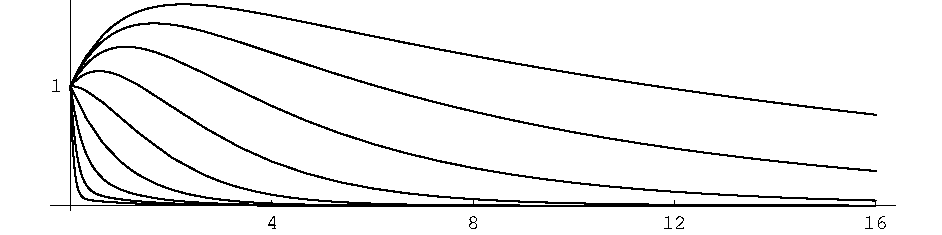
\includegraphics[width=\textwidth]{ode/first_order/range_alpha}
    \end{center}
    \caption{The solution for a range of values of the parameter.}
    \label{figure range alpha}
  \end{figure}

  Consider the solution in the limit as $\alpha \to 0$.
  \begin{align*}
    \lim_{\alpha \to 0} y(x)
    &= \lim_{\alpha \to 0} \frac{1}{\alpha - 1} \left( \e^{-x} 
      + (\alpha-2) \e^{- \alpha x} \right) \\
    &= 2 - \e^{-x}
  \end{align*}
  In the limit as $\alpha \to \infty$ we have,
  \begin{align*}
    \lim_{\alpha \to \infty} y(x)
    &= \lim_{\alpha \to \infty} \frac{1}{\alpha - 1} \left( \e^{-x} 
      + (\alpha-2) \e^{- \alpha x} \right) \\
    &= \lim_{\alpha \to \infty} \frac{\alpha-2}{\alpha - 1} 
    \e^{- \alpha x} \\
    &= \begin{cases}
      1 & \mathrm{for}\ x = 0, \\
      0 & \mathrm{for}\ x > 0.
    \end{cases}
  \end{align*}
  This behavior is shown in Figure~\ref{alpha_0_alpha_inf}.  The first graph
  plots the solutions for $\alpha = 1/128, 1/64, \ldots,1$.
  The second graph plots the solutions for 
  $\alpha = 1,2,\ldots,128$.

  \begin{figure}[tb!]
    \begin{center}
      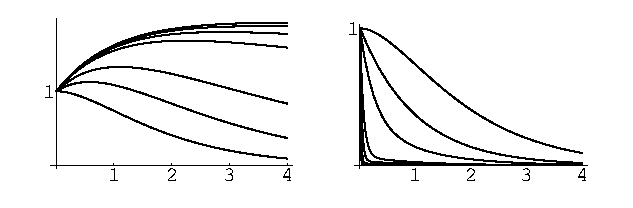
\includegraphics[width=0.7\textwidth]{ode/first_order/alpha_0_alpha_inf}
    \end{center}
    \caption{The solution for limiting values of the parameter.}
    \label{alpha_0_alpha_inf}
  \end{figure}
\end{Solution}







%% Taylor series about origin
\begin{Solution} 
  \label{solution dwdz + 1 1-z w}
  We substitute $w = \sum_{n=0}^\infty a_n z^n$ into the equation 
  $\frac{\dd w}{\dd z} + \frac{1}{1-z} w = 0$.
  \begin{gather*}
    \frac{\dd}{\dd z} \sum_{n=0}^\infty a_n z^n 
    + \frac{1}{1-z}\sum_{n=0}^\infty a_n z^n = 0 \\
    (1-z)\sum_{n=1}^\infty n a_n z^{n-1} + \sum_{n=0}^\infty a_n z^n = 0 \\
    \sum_{n=0}^\infty (n+1) a_{n+1} z^n - \sum_{n=0}^\infty n a_n z^n
    + \sum_{n=0}^\infty a_n z^n = 0 \\
    \sum_{n=0}^\infty \left( (n+1) a_{n+1} - (n-1) a_n \right) z^n = 0
  \end{gather*}
  Equating powers of $z$ to zero, we obtain the relation,
  \[
  a_{n+1} = \frac{n-1}{n+1} a_n.
  \]
  $a_0$ is arbitrary.  We can compute the rest of the coefficients from the 
  recurrence relation.
  \begin{align*}
    &a_1 = \frac{-1}{1} a_0 = -a_0 \\
    &a_2 = \frac{0}{2} a_1 = 0
  \end{align*}
  We see that the coefficients are zero for $n \geq 2$. Thus the Taylor
  series expansion, (and the exact solution),  is
  \[ 
  \boxed{
    w = a_0(1-z).
    } 
  \]
  The radius of convergence of the series in infinite.  The nearest singularity
  of $\frac{1}{1-z}$ is at $z=1$.  Thus we see the radius of convergence can
  be greater than the distance to the nearest singularity of the coefficient 
  function, $p(z)$.
\end{Solution}








\solutions{

  %%-----------------------------------------------------------------------------
  \begin{large}
    \noindent
    \textbf{Exact Equations}
  \end{large}




  \begin{Solution}
    \label{solution dydx=xxyyx}
    \begin{enumerate}
      %%
      %%
    \item
      \[
      \frac{\dd y}{\dd x} = \frac{ x^2 + x y + y^2 }{ x^2 }
      \]
      Since the right side is a homogeneous function of order zero, this is a 
      homogeneous differential equation.  We make the change of variables
      $u = y / x$ and then solve the differential equation for $u$.
      \begin{gather*}
        x u' + u = 1 + u + u^2 \\
        \frac{ \dd u }{ 1 + u^2 } = \frac{ \dd x }{ x } \\
        \arctan(u) = \ln |x| + c \\
        u = \tan( \ln(|c x|) ) \\
        \boxed{
          y = x \tan( \ln(|c x|) )
          }
      \end{gather*}
      %%
      %%
    \item
      \[
      (4y-3x) \,\dd x + (y-2x) \,\dd y = 0
      \]
      Since the coefficients are homogeneous functions of order one, this is a 
      homogeneous differential equation.  We make the change of variables
      $u = y / x$ and then solve the differential equation for $u$.
      \begin{gather*}
        \left( 4 \frac{y}{x} - 3 \right) \,\dd x 
        + \left( \frac{y}{x} - 2 \right) \,\dd y = 0 \\
        (4 u - 3) \,\dd x + (u - 2)(u \,\dd x + x \,\dd u) = 0 \\
        (u^2 + 2 u - 3) \,\dd x + x (u - 2) \,\dd u  = 0 \\
        \frac{\dd x}{x} + \frac{u - 2}{(u+3)(u-1)} \,\dd u = 0 \\
        \frac{\dd x}{x} 
        + \left( \frac{5/4}{u+3} - \frac{1/4}{u-1} \right) \,\dd u = 0 \\
        \ln(x) + \frac{5}{4} \ln(u+3) - \frac{1}{4} \ln(u-1) = c \\
        \frac{ x^4 (u+3)^5 }{ u-1 } = c \\
        \frac{ x^4 (y/x + 3)^5 }{ y/x - 1 } = c \\
        \boxed{
          \frac{ (y + 3 x)^5 }{ y - x } = c
          }
      \end{gather*}
    \end{enumerate}
  \end{Solution}








  \begin{Solution}
    \label{solution dydx=axbybxcy}
    \begin{enumerate}
      %%
      %%
    \item
      \[
      (3x^2-2xy+2) \,\dd x+(6y^2-x^2+3) \,\dd y = 0
      \]
      We check if this form of the equation, $P \,\dd x + Q \,\dd y = 0$, is exact.
      \[
      P_y = - 2 x, \qquad Q_x = -2 x
      \]
      Since $P_y = Q_x$, the equation is exact.  Now we find the primitive
      $u(x,y)$ which satisfies 
      \[
      \dd u = (3x^2-2xy+2) \,\dd x+(6y^2-x^2+3) \,\dd y.
      \]
      The primitive satisfies the partial differential equations
      \begin{equation}
        \label{ux=P,uy=Q}
        u_x = P, \quad u_y = Q.
      \end{equation}
      We integrate the first equation of~\ref{ux=P,uy=Q} to determine $u$ up 
      to a function of integration.
      \begin{gather*}
        u_x = 3 x^2 - 2 x y + 2 \\
        u = x^3 - x^2 y + 2 x + f(y)
      \end{gather*}
      We substitute this into the second equation of~\ref{ux=P,uy=Q} to determine
      the function of integration up to an additive constant.
      \begin{gather*}
        -x^2 + f'(y) = 6 y^2 - x^2 + 3 \\
        f'(y) = 6 y^2 + 3 \\
        f(y) = 2 y^3 + 3 y
      \end{gather*}
      The solution of the differential equation is determined by the 
      implicit equation $u = c$.
      \[
      \boxed{
        x^3 - x^2 y + 2 x + 2 y^3 + 3 y = c
        }
      \]
      %%
      %%
    \item
      \begin{gather*}
        \frac{\dd y}{\dd x} = - \frac{ax+by}{bx+cy} \\
        ( a x + b y ) \,\dd x + ( b x + c y ) \,\dd y = 0
      \end{gather*}
      We check if this form of the equation, $P \,\dd x + Q \,\dd y = 0$, is exact.
      \[
      P_y = b, \qquad Q_x = b
      \]
      Since $P_y = Q_x$, the equation is exact.  Now we find the primitive
      $u(x,y)$ which satisfies 
      \[
      \dd u = ( a x + b y ) \,\dd x + ( b x + c y ) \,\dd y
      \]
      The primitive satisfies the partial differential equations
      \begin{equation}
        \label{ux=P,uy=Q2}
        u_x = P, \quad u_y = Q.
      \end{equation}
      We integrate the first equation of~\ref{ux=P,uy=Q2} to determine $u$ up 
      to a function of integration.
      \begin{gather*}
        u_x = a x + b y \\
        u = \frac{1}{2} a x^2 + b x y + f(y)
      \end{gather*}
      We substitute this into the second equation of~\ref{ux=P,uy=Q2} to determine
      the function of integration up to an additive constant.
      \begin{gather*}
        b x + f'(y) = b x + c y \\
        f'(y) = c y \\
        f(y) = \frac{1}{2} c y^2
      \end{gather*}
      The solution of the differential equation is determined by the 
      implicit equation $u = d$.
      \[
      \boxed{
        a x^2 + 2 b x y + c y^2 = d
        }
      \]
    \end{enumerate}
  \end{Solution}










  \begin{Solution}
    \label{solution dydx = 1-2x y2}
    Note that since these equations are nonlinear, we cannot predict where the 
    solutions will be defined from the equation alone.
    \begin{enumerate}
      %%
      %%
    \item
      This equation is separable.  We integrate to get the general solution.
      \begin{gather*}
        \frac{\dd y}{\dd x} = (1-2x) y^2 \\
        \frac{\dd y}{y^2} = (1 - 2 x) \,\dd x \\
        - \frac{1}{y} = x - x^2 + c \\
        y = \frac{1}{x^2 - x - c}
      \end{gather*}
      Now we apply the initial condition.
      \begin{gather*}
        y(0) = \frac{1}{-c} = - \frac{1}{6} \\
        y = \frac{1}{x^2 - x - 6} \\
        \boxed{
          y = \frac{1}{(x+2)(x-3)}
          }
      \end{gather*}
      The solution is defined on the interval $(-2 \ldots 3)$.
      %%
      %%
    \item
      This equation is separable.  We integrate to get the general solution.
      \begin{gather*}
        x \,\dd x + y \e^{-x} \,\dd y = 0 \\
        x \e^x \,\dd x + y \,\dd y = 0 \\
        (x - 1) \e^x + \frac{1}{2} y^2 = c \\
        y = \sqrt{ 2 ( c + (1-x) \e^x ) }
      \end{gather*}
      We apply the initial condition to determine the constant of integration.
      \begin{gather*}
        y(0) = \sqrt{ 2 (c + 1) }= 1 \\
        c = - \frac{1}{2} \\
        \boxed{
          y = \sqrt{ 2 (1-x) \e^x - 1 }
          }
      \end{gather*}
      The function $2(1-x) \e^x - 1$ is plotted in Figure~\ref{21xex1}.  We see that
      the argument of the square root in the solution is non-negative only on 
      an interval about the origin.  Because $2 (1-x) \e^x - 1 == 0$ is a mixed
      algebraic / transcendental equation, we cannot solve it analytically.  The
      solution of the differential equation is defined on the interval
      $(-1.67835 \ldots 0.768039)$.

      \begin{figure}[tb!]
        \begin{center}
          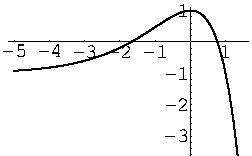
\includegraphics[width=0.25\textwidth]{ode/first_order/21xex1}
        \end{center}
        \caption{The function.}
        \label{21xex1}
      \end{figure}
    \end{enumerate}
  \end{Solution}










  %% (4 y - x) y' - (9 x^2 + y - 1) = 0.
  \begin{Solution}
    \label{solution 4yxy9x2y10}
    \begin{enumerate}
      %%
      %%
    \item
      We consider the differential equation,
      \[
      (4 y - x) y' - (9 x^2 + y - 1) = 0.
      \]
      \begin{gather*}
        P_y = \frac{\partial}{\partial y} \left( 1 - y - 9 x^2 \right) = -1 \\
        Q_x = \frac{\partial}{\partial x} \left( 4 y - x \right) = -1
      \end{gather*}
      This equation is exact.  It is simplest to solve the equation by rearranging
      terms to form exact derivatives.
      \begin{gather*}
        4 y y' - x y' - y + 1 - 9 x^2 = 0 \\
        \frac{\dd}{\dd x} \left[ 2 y^2 - x y \right] + 1 - 9 x^2 = 0 \\
        2 y^2 - x y + x - 3 x^3 + c = 0 \\
        \boxed{
          y = \frac{1}{4} \left( x \pm \sqrt{x^2 - 8 ( c + x - 3 x^3 ) } \right)
          }
      \end{gather*}
      %%
      %%
    \item
      We consider the differential equation,
      \[
      (2 x - 2 y) y' + (2 x + 4 y) = 0.
      \]
      \begin{gather*}
        P_y = \frac{\partial}{\partial y} \left( 2 x + 4 y \right) = 4 \\
        Q_x = \frac{\partial}{\partial x} \left( 2 x - 2 y \right) = 2
      \end{gather*}
      Since $P_y \neq Q_x$, this is not an exact equation.
    \end{enumerate}
  \end{Solution}










  %% y^2 \sin t + y f(t) \frac{\dd y}{\dd t} = 0
  \begin{Solution}
    \label{solution y2 sin t + y f dydt}
    Recall that the differential equation
    \[
    P(x, y) + Q(x, y) y' = 0
    \]
    is exact if and only if $P_y = Q_x$.
    For Equation~\ref{eqn_y2_sint}, this criterion is 
    \begin{gather*}
      2 y \sin t = y f'(t) \\
      f'(t) = 2 \sin t \\
      \boxed{
        f(t) = 2(a - \cos t).
        }
    \end{gather*}
    In this case, the differential equation is
    \[
    y^2 \sin t + 2 y y' (a - \cos t) = 0.
    \]
    We can integrate this exact equation by inspection.
    \begin{gather*}
      \frac{\dd}{\dd t} \left( y^2 (a - \cos t) \right) = 0 \\
      y^2 (a - \cos t) = c \\
      \boxed{
        y = \pm \frac{c}{ \sqrt{ a - \cos t } }
        }
    \end{gather*}
  \end{Solution}









  %%-----------------------------------------------------------------------------
  \begin{large}
    \noindent
    \textbf{The First Order, Linear Differential Equation}
  \end{large}





  %% y' + \frac{y}{\sin x} = 0. 
  \begin{Solution}
    \label{solution y + y / sin x}
    Consider the differential equation
    \[ 
    y' + \frac{y}{\sin x} = 0. 
    \]
    We use Equation~\ref{first order linear homogeneous} to determine 
    the solution.
    \begin{gather*}
      y = c \e^{ \int -1/\sin x \,\dd x } 
      \\
      y = c \e^{ - \ln | \tan (x/2) | } 
      \\
      y = c \left| \cot \left( \frac{x}{2} \right) \right| 
      \\
      \boxed{ 
        y = c \cot \left( \frac{x}{2} \right)
        } 
    \end{gather*}
  \end{Solution}












  %%-----------------------------------------------------------------------------
  \begin{large}
    \noindent
    \textbf{Initial Conditions}
  \end{large}







  %%-----------------------------------------------------------------------------
  \begin{large}
    \noindent
    \textbf{Well-Posed Problems}
  \end{large}






  %% t \frac{\dd y}{\dd t} + A y = 1 + t^2
  \begin{Solution}
    \label{solution t dydt + A y}
    First we write the differential equation in the standard form.
    \[
    \frac{\dd y}{\dd t} + \frac{A}{t} y = \frac{1}{t} + t, \quad t > 0
    \]
    We determine the integrating factor.
    \[
    I(t) = \e^{\int A / t \,\dd t} = \e^{A \ln t} = t^A
    \]
    We multiply the differential equation by the
    integrating factor and integrate.
    \begin{gather*}
      \frac{\dd y}{\dd t} + \frac{A}{t} y = \frac{1}{t} + t 
      \\
      \frac{\dd}{\dd t} \left( t^A y \right) = t^{A-1} + t^{A+1} 
      \\
      t^A y = \begin{cases}
        \frac{t^A}{A} + \frac{t^{A+2}}{A+2} + c, &A \neq 0, -2 
        \\
        \ln t + \frac{1}{2} t^2 + c, &A = 0 
        \\
        - \frac{1}{2} t^{-2} + \ln t + c, &A = -2
      \end{cases} 
      \\
      y = \begin{cases}
        \frac{1}{A} + \frac{t^2}{A+2} + c t^{-A}, &A \neq -2 
        \\
        \ln t + \frac{1}{2} t^2 + c, &A = 0 
        \\
        - \frac{1}{2} + t^2 \ln t + c t^2, &A = -2
      \end{cases}
    \end{gather*}
    For positive $A$, the solution is bounded at the origin only for $c = 0$.
    For $A = 0$, there are no bounded solutions.
    For negative $A$, the solution is bounded there for any value of $c$ and 
    thus we have a one-parameter family of solutions.

    In summary, the solutions which are bounded at the origin are:
    \[
    \boxed{
      y =
      \begin{cases}
        \frac{1}{A} + \frac{t^2}{A+2}, &A > 0 
        \\
        \frac{1}{A} + \frac{t^2}{A+2} + c t^{-A}, &A < 0,\ A \neq -2 
        \\
        - \frac{1}{2} + t^2 \ln t + c t^2, &A = -2
      \end{cases}
      }
    \]
  \end{Solution}






  %%-----------------------------------------------------------------------------
  \begin{large}
    \noindent
    \textbf{Equations in the Complex Plane}
  \end{large}




  %% Classify the singular points of the following first order differential
  \begin{Solution}  
    \label{solution dwdz + sin z z w}

    $\phantom{a}$   %% Used to force a new paragraph.

    \begin{enumerate}
      %%
    \item Consider the equation $w' + \frac{\sin z}{z} w = 0$.  
      The point $z=0$ is the only point we need to examine in the finite plane.
      Since $\frac{\sin z}{z}$ has a removable singularity at $z=0$, there are 
      no singular points in the finite plane.
      The substitution $z = \frac{1}{\zeta}$ yields the equation
      \[ 
      u' - \frac{\sin(1/\zeta)}{\zeta}u = 0.
      \]
      Since $\frac{\sin(1/\zeta)}{\zeta}$ has an essential singularity at 
      $\zeta = 0$, the point at infinity is an irregular singular point of the 
      original differential equation.
      %%
    \item Consider the equation $w' + \frac{1}{z-3} w = 0$.
      Since $\frac{1}{z-3}$ has a simple pole at $z=3$, the differential equation
      has a regular singular point there.  Making the substitution 
      $z = 1/\zeta$, $w(z)=u(\zeta)$
      \begin{gather*}
        u' - \frac{1}{\zeta^2(1/\zeta-3)} u  = 0 \\
        u' - \frac{1}{\zeta(1-3\zeta)} u = 0.
      \end{gather*}
      Since this equation has a simple pole at $\zeta = 0$, the original equation 
      has a regular singular point at infinity.
      %%
    \item Consider the equation $w' + z^{1/2} w = 0$.
      There is an irregular singular point at $z = 0$.  With the substitution
      $z = 1/\zeta$, $w(z) = u(\zeta)$,
      \begin{gather*}
        u' - \frac{\zeta^{-1/2}}{\zeta^2} u = 0 \\
        u' - \zeta^{-5/2} u = 0.
      \end{gather*}
      We see that the point at infinity is also an irregular singular point
      of the original differential equation.
    \end{enumerate}
  \end{Solution}







  %% Expand irregular singular point in a Frobenius series.
  \begin{Solution} 
    \label{solution dwdz z-2 w}
    We start with the equation
    \[ 
    w' + z^{-2}w = 0.
    \]
    Substituting $w = z^\lambda \sum_{n=0}^\infty a_n z^n$, $a_0 \neq 0$ yields
    \begin{gather*}
      \frac{\dd}{\dd z} \left(z^\lambda \sum_{n=0}^\infty a_n z^n\right) + 
      z^{-2}z^\lambda \sum_{n=0}^\infty a_n z^n = 0 \\
      \lambda z^{\lambda-1} \sum_{n=0}^\infty a_n z^n 
      + z^\lambda \sum_{n=1}^\infty n a_n z^{n-1}
      + z^\lambda \sum_{n=0}^\infty a_n z^{n-2} = 0
    \end{gather*}
    The lowest power of $z$ in the expansion is $z^{\lambda-2}$.  The 
    coefficient of this term is $a_0$.  Equating powers of $z$ demands that
    $a_0 = 0$ which contradicts our initial assumption that it was nonzero.
    Thus we cannot find a $\lambda$ such that the solution can be expanded
    in the form,
    \[ 
    w = z^\lambda \sum_{n=0}^\infty a_n z^n, \qquad a_0 \neq 0.
    \]
  \end{Solution}

  

\raggedbottom
}
%%=============================================================================
\pagebreak
\flushbottom
\section{Quiz}


\begin{QuizProblem}
  \label{quiz problem general solution first order}
  What is the \textit{general solution} of a first order 
  differential equation?

  \quizsolution{general solution first order}
\end{QuizProblem}


\begin{QuizProblem}
  \label{quiz problem first order exact separable}
  Write a statement about the functions $P$ and $Q$ to make the following 
  statement correct.

  The first order differential equation
  \[
  P(x, y) + Q(x, y) \frac{\dd y}{\dd x} = 0
  \]
  is exact if and only if $\underline{\phantom{P_y = Q_x}}$.
  It is separable if $\underline{\phantom{P = P(x) and Q = Q(y)}}$.

  \quizsolution{first order exact separable}
\end{QuizProblem}


\begin{QuizProblem}
  \label{quiz problem y' + p y = f}
  Derive the general solution of
  \[
  \frac{\dd y}{\dd x} + p(x) y = f(x).
  \]

  \quizsolution{y' + p y = f}
\end{QuizProblem}


\begin{QuizProblem}
  \label{quiz problem y' = y + y2}
  Solve $y' = y - y^2$.

  \quizsolution{y' = y + y2}
\end{QuizProblem}








\raggedbottom
%%=============================================================================
\pagebreak
\flushbottom
\section{Quiz Solutions}


\begin{QuizSolution}
  \label{quiz solution general solution first order}
  The general solution of a first order differential equation is a 
  one-parameter family of functions which satisfies the equation.
\end{QuizSolution}


\begin{QuizSolution}
  \label{quiz solution first order exact separable}
  The first order differential equation
  \[
  P(x, y) + Q(x, y) \frac{\dd y}{\dd x} = 0
  \]
  is exact if and only if $P_y = Q_x$.
  It is separable if $P = P(x)$ and $Q = Q(y)$.
\end{QuizSolution}


\begin{QuizSolution}
  \label{quiz solution y' + p y = f}
  \[
  \frac{\dd y}{\dd x} + p(x) y = f(x)
  \]
  We multiply by the integrating factor 
  $\mu(x) = \exp(P(x)) = \exp\left( \int p(x) \,\dd x \right)$, and integrate.
  \begin{gather*}
    \frac{\dd y}{\dd x} \e^{P(x)} + p(x) y \e^{P(x)} = \e^{P(x)} f(x) 
    \\
    \frac{\dd}{\dd x} \left( y \e^{P(x)} \right) = \e^{P(x)} f(x) 
    \\
    y \e^{P(x)} = \int \e^{P(x)} f(x)\,\dd x + c 
    \\
    y = \e^{-P(x)} \int \e^{P(x)} f(x)\,\dd x + c \e^{-P(x)}
  \end{gather*}
\end{QuizSolution}


\begin{QuizSolution}
  \label{quiz solution y' = y + y2}
  $y' = y - y^2$ is separable.
  \begin{gather*}
    y' = y - y^2 
    \\
    \frac{y'}{y - y^2} = 1 
    \\
    \frac{y'}{y} - \frac{y'}{y - 1} = 1 
    \\
    \ln y - \ln(y - 1) = x + c 
    \\
    \intertext{We do algebraic simplifications and rename the constant 
      of integration to write the solution in a nice form.}
    \frac{y}{y-1} = c \e^x 
    \\
    y = (y - 1) c \e^x 
    \\
    y = \frac{-c \e^x}{1 - c \e^x} 
    \\
    y = \frac{\e^x}{\e^x - c} 
    \\
    y = \frac{1}{1 - c \e^{-x}} 
  \end{gather*}
\end{QuizSolution}










\raggedbottom


\flushbottom

%% CONTINUE: Needs a lot of work.



%%============================================================================
%%============================================================================
\chapter{First Order Linear Systems of Differential Equations}



We all agree that your theory is crazy, but is it crazy enough?

\begin{flushright}
  - Niels Bohr 
\end{flushright}




%%=============================================================================
\section{Introduction}



%% CONTINUE: Motivating example.


In this chapter we consider first order linear systems of differential 
equations.  That is, we consider equations of the form,
\begin{gather*}
  \mathbf{x}'(t) = \mathbf{A} \mathbf{x}(t) + \mathbf{f}(t),
  \\
  \mathbf{x}(t) = \begin{pmatrix} x_1(t) \\ \vdots \\ x_n(t) \end{pmatrix},
  \qquad
  \mathbf{A} = 
  \begin{pmatrix}
    a_{11}       & a_{12}     & \ldots        &a_{1n} \\
    a_{21}       & a_{22}     & \ldots        &a_{2n} \\
    \vdots          & \vdots        & \ddots        & \vdots \\
    a_{n1}       & a_{n2}     & \ldots        &a_{nn}
  \end{pmatrix}.
\end{gather*}
Initially we will consider the homogeneous problem, 
$\mathbf{x}'(t) = \mathbf{A} \mathbf{x}(t)$.  (Later we will find particular solutions with 
variation of parameters.)  The best way to solve these equations is through
the use of the matrix exponential.  Unfortunately, using the matrix 
exponential requires knowledge of the Jordan canonical form and matrix 
functions.  Fortunately, we can solve a certain class of problems using 
only the concepts of eigenvalues and eigenvectors of a matrix.  We present
this simple method in the next section.  In the following section
we will take a detour into
matrix theory to cover Jordan canonical form and its applications.  Then
we will be able to solve the general case.









%%=============================================================================
\section{Using Eigenvalues and Eigenvectors to find Homogeneous Solutions}







If you have forgotten what eigenvalues and eigenvectors are and how to compute
them, go find
a book on linear algebra and spend a few minutes re-aquainting yourself 
with the rudimentary material.
%% CONTINUE: add linear algebra to the book.


Recall that the single differential equation $x'(t) = A x$ has the general
solution $x = c \e^{A t}$.  Maybe the system of differential equations 
\begin{equation}
  \label{eq:x'=Ax}
  \mathbf{x}'(t) = \mathbf{A} \mathbf{x}(t)
\end{equation}
has similiar solutions.  Perhaps it has a solution
of the form $\mathbf{x}(t) = \boldsymbol{\xi} \e^{\lambda t}$ for some constant vector $\boldsymbol{\xi}$ and 
some value $\lambda$.  Let's substitute this into the differential equation
and see what happens.
\begin{gather*}
  \mathbf{x}'(t) = \mathbf{A} \mathbf{x}(t)
  \\
  \boldsymbol{\xi} \lambda \e^{\lambda t} = \mathbf{A} \boldsymbol{\xi} \e^{\lambda t}
  \\
  \mathbf{A} \boldsymbol{\xi} = \lambda \boldsymbol{\xi}
\end{gather*}
We see that if $\lambda$ is an eigenvalue of $\mathbf{A}$ with eigenvector $\boldsymbol{\xi}$
then $\mathbf{x}(t) = \boldsymbol{\xi} \e^{\lambda t}$ satisfies the differential equation.  Since 
the differential equation is linear, $c \boldsymbol{\xi} \e^{\lambda t}$ is a solution.

Suppose that the $n \times n$ matrix $\mathbf{A}$ has the eigenvalues $\{ \lambda_k \}$ 
with a complete
set of linearly independent eigenvectors $\{ \boldsymbol{\xi}_k \}$.  Then each of
$\boldsymbol{\xi}_k \e^{\lambda_k t}$ is a homogeneous solution of Equation~\ref{eq:x'=Ax}.
We note that each of these solutions is linearly independent.  Without
any kind of justification I will tell you that the general solution of
the differential equation is a linear combination of these $n$ linearly 
independent solutions.
%% CONTINUE



\begin{Result}
  Suppose that the $n \times n$ matrix $\mathbf{A}$ has the eigenvalues $\{ \lambda_k \}$ 
  with a complete set of linearly independent eigenvectors $\{ \boldsymbol{\xi}_k \}$.
  The system of differential equations,
  \[
  \mathbf{x}'(t) = \mathbf{A} \mathbf{x}(t),
  \]
  has the general solution,
  \[
  \mathbf{x}(t) = \sum_{k = 1}^n c_k \boldsymbol{\xi}_k \e^{\lambda_k t}
  \]
\end{Result}




%% CONTINUE WRITE MORE





\begin{Example}[mathematica/ode/systems/systems.nb]
  Find the solution of the following initial value problem.
  Describe the behavior of the solution as $t \to \infty$.
  \[
  \mathbf{x}' = \mathbf{A} x \equiv
  \begin{pmatrix}
    -2 & 1\\
    -5 & 4
  \end{pmatrix} 
  \mathbf{x}, \quad 
  \mathbf{x}(0) = \mathbf{x}_0 \equiv
  \begin{pmatrix}
    1\\
    3
  \end{pmatrix}
  \]

  The matrix has the distinct eigenvalues $\lambda_1 = -1$, $\lambda_2 = 3$.  The 
  corresponding eigenvectors are 
  \[
  \mathbf{x}_1 = \begin{pmatrix} 1 \\ 1 \end{pmatrix}, \quad
  \mathbf{x}_2 = \begin{pmatrix} 1 \\ 5 \end{pmatrix}.
  \]
  The general solution of the system of differential equations is
  \[
  \mathbf{x} = 
  c_1 \begin{pmatrix} 1 \\ 1 \end{pmatrix} \e^{-t}
  + c_2 \begin{pmatrix} 1 \\ 5 \end{pmatrix} \e^{3 t}.
  \]
  We apply the initial condition to determine the constants.
  \begin{gather*}
    \begin{pmatrix}
      1 & 1 \\
      1 & 5
    \end{pmatrix}
    \begin{pmatrix}
      c_1 \\
      c_2
    \end{pmatrix}
    =
    \begin{pmatrix}
      1 \\
      3
    \end{pmatrix} \\
    c_1 = \frac{1}{2}, \quad c_2 = \frac{1}{2}
  \end{gather*}
  The solution subject to the initial condition is
  \[
  \boxed{
    \mathbf{x} = 
    \frac{1}{2} \begin{pmatrix} 1 \\ 1 \end{pmatrix} \e^{-t}
    + \frac{1}{2} \begin{pmatrix} 1 \\ 5 \end{pmatrix} \e^{3 t}
    }
  \]
  For large $t$, the solution looks like
  \[
  \mathbf{x} \approx \frac{1}{2} \begin{pmatrix} 1 \\ 5 \end{pmatrix} \e^{3 t}.
  \]
  Both coordinates tend to infinity.

  Figure~\ref{x_2154x} shows some homogeneous solutions in the phase plane.
  \begin{figure}[tb!]
    \begin{center}
      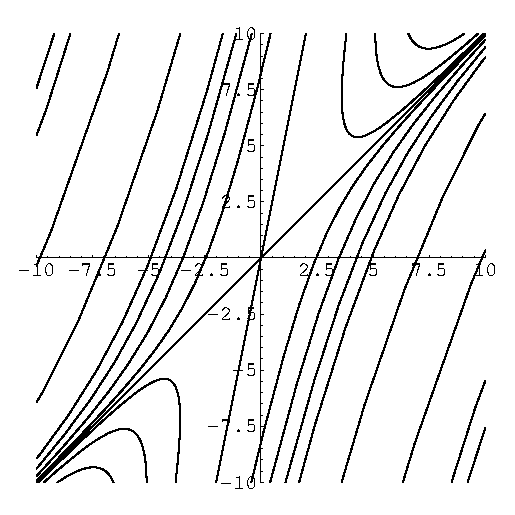
\includegraphics[width=0.4\textwidth]{ode/systems/x_2154x}
    \end{center}
    \caption{Homogeneous solutions in the phase plane.}
    \label{x_2154x}
  \end{figure}
\end{Example}











\begin{Example}[mathematica/ode/systems/systems.nb]
  Find the solution of the following initial value problem.
  Describe the behavior of the solution as $t \to \infty$.
  \[
  \mathbf{x}' = \mathbf{A} x \equiv
  \begin{pmatrix}
    1 & 1 & 2 \\
    0 & 2 & 2 \\
    -1 & 1 & 3
  \end{pmatrix} 
  \mathbf{x}, \quad 
  \mathbf{x}(0) = \mathbf{x}_0 \equiv
  \begin{pmatrix}
    2 \\
    0 \\
    1
  \end{pmatrix}
  \]

  The matrix has the distinct eigenvalues $\lambda_1 = 1$, $\lambda_2 = 2$, $\lambda_3 = 3$.  The 
  corresponding eigenvectors are 
  \[
  \mathbf{x}_1 = \begin{pmatrix} 0 \\ -2 \\ 1 \end{pmatrix}, \quad
  \mathbf{x}_2 = \begin{pmatrix} 1 \\ 1 \\ 0 \end{pmatrix}, \quad
  \mathbf{x}_3 = \begin{pmatrix} 2 \\ 2 \\ 1 \end{pmatrix}.
  \]
  The general solution of the system of differential equations is
  \[
  \mathbf{x} = 
  c_1 \begin{pmatrix} 0 \\ -2 \\ 1 \end{pmatrix} \e^t
  + c_2 \begin{pmatrix} 1 \\ 1 \\ 0 \end{pmatrix} \e^{2 t}
  + c_3 \begin{pmatrix} 2 \\ 2 \\ 1 \end{pmatrix} \e^{3 t}.
  \]
  We apply the initial condition to determine the constants.
  \begin{gather*}
    \begin{pmatrix}
      0 & 1 & 2 \\
      -2 & 1 & 2 \\
      1 & 0 & 1
    \end{pmatrix}
    \begin{pmatrix}
      c_1 \\
      c_2 \\
      c_3
    \end{pmatrix}
    =
    \begin{pmatrix}
      2 \\
      0 \\
      1
    \end{pmatrix} \\
    c_1 = 1, \quad c_2 = 2, \quad c_3 = 0
  \end{gather*}
  The solution subject to the initial condition is
  \[
  \boxed{
    \mathbf{x} = 
    \begin{pmatrix} 0 \\ -2 \\ 1 \end{pmatrix} \e^t
    + 2 \begin{pmatrix} 1 \\ 1 \\ 0 \end{pmatrix} \e^{2 t}.
    }
  \]
  As $t \to \infty$, all coordinates tend to infinity.
\end{Example}







\begin{Exercise}[mathematica/ode/systems/systems.nb]
  \label{exercise x'=(1-51-3)x t-infinity}
  Find the solution of the following initial value problem.
  Describe the behavior of the solution as $t \to \infty$.
  \[
  \mathbf{x}' = \mathbf{A} x \equiv
  \begin{pmatrix}
    1 & -5 \\
    1 & -3
  \end{pmatrix} 
  \mathbf{x}, \quad 
  \mathbf{x}(0) = \mathbf{x}_0 \equiv
  \begin{pmatrix}
    1 \\
    1
  \end{pmatrix}
  \]

  \hintsolution{x'=(1-51-3)x t-infinity}
\end{Exercise}




\begin{Exercise}[mathematica/ode/systems/systems.nb]
  \label{exercise x'=(-3021-10-2-10)x t-infinity}
  Find the solution of the following initial value problem.
  Describe the behavior of the solution as $t \to \infty$.
  \[
  \mathbf{x}' = \mathbf{A} x \equiv
  \begin{pmatrix}
    -3 & 0 & 2 \\
    1 & -1 & 0 \\
    -2 & -1 & 0
  \end{pmatrix} 
  \mathbf{x}, \quad 
  \mathbf{x}(0) = \mathbf{x}_0 \equiv
  \begin{pmatrix}
    1 \\
    0 \\
    0
  \end{pmatrix}
  \]

  \hintsolution{x'=(-3021-10-2-10)x t-infinity}
\end{Exercise}




%% Use the matrix form of the method of variation of parameters to find the 
\begin{Exercise}
  \label{exercise dxdt=4284x+t3t2}
  Use the matrix form of the method of variation of parameters to find the 
  general solution of
  \[
  \frac{\dd \mathbf{x}}{\dd t} = 
  \begin{pmatrix}
    4 & -2 \\
    8 & -4
  \end{pmatrix}
  \mathbf{x} + 
  \begin{pmatrix}
    t^{-3} \\
    -t^{-2}
  \end{pmatrix},
  \quad t > 0.
  \]

  \hintsolution{dxdt=4284x+t3t2}
\end{Exercise}








%%=============================================================================
\section{Matrices and Jordan Canonical Form} 


%% CONTINUE: convergence
\paragraph{Functions of Square Matrices.}
Consider a function $f(x)$ with a Taylor series.
\[
f(x) = \sum_{n = 0}^\infty \frac{f^{(n)}(0)}{n!} x^n
\]
We can define the function to take square matrices as arguments.
The function of the square matrix $\mathbf{A}$ is defined in terms of the 
Taylor series.
\[
f(\mathbf{A}) = \sum_{n = 0}^\infty \frac{f^{(n)}(0)}{n!} \mathbf{A}^n
\]
(Note that this definition is usually not the most convenient method
for computing a function of a matrix.  Use the Jordan canonical form for
that.)






\paragraph{Eigenvalues and Eigenvectors.}
Consider a square matrix $\mathbf{A}$.
A nonzero vector $\mathbf{x}$ is an \textit{eigenvector} of the matrix with 
\textit{eigenvalue} $\lambda$ if 
\[
\mathbf{A} \mathbf{x} = \lambda \mathbf{x}.
\]
Note that we can write this equation as
\[
(\mathbf{A} - \lambda \mathbf{I}) \mathbf{x} = \mathbf{0}.
\]
This equation has solutions for nonzero $\mathbf{x}$ if and only if 
$\mathbf{A} - \lambda \mathbf{I}$ is singular, ($\det(\mathbf{A} - \lambda \mathbf{I}) = 0$).
We define the \textit{characteristic polynomial} of the matrix $\chi(\lambda)$ as 
this determinant.
\[
\chi(\lambda) = \det(\mathbf{A} - \lambda \mathbf{I})
\]
The roots of the characteristic polynomial are the eigenvalues of the matrix.
The eigenvectors of distinct eigenvalues are linearly independent.  
Thus if a matrix has distinct eigenvalues, the eigenvectors form a basis.

If $\lambda$ is a root of $\chi(\lambda)$ of multiplicity $m$ then there 
are up to $m$ linearly independent eigenvectors corresponding to that 
eigenvalue.  That is, it has from $1$ to $m$ eigenvectors.





\paragraph{Diagonalizing Matrices.}
Consider an $n \times n$ matrix $\mathbf{A}$ that has a complete set of $n$ 
linearly independent eigenvectors.  $\mathbf{A}$ may or may not have distinct
eigenvalues.  Consider the matrix $\mathbf{S}$ with eigenvectors as columns.
\[
\mathbf{S} =
\begin{pmatrix}
  \mathbf{x}_1 & \mathbf{x}_2 & \cdots & \mathbf{x}_n 
\end{pmatrix}
\]
$\mathbf{A}$ is diagonalized by the similarity transformation:
\[
\boldsymbol{\Lambda} = \mathbf{S}^{-1} \mathbf{A} \mathbf{S}.
\]
$\boldsymbol{\Lambda}$ is a diagonal matrix with the eigenvalues of $\mathbf{A}$ as the 
diagonal elements.  Furthermore, the $k^{\mathrm{th}}$ diagonal element
is $\lambda_k$, the eigenvalue corresponding to the the eigenvector,
$\mathbf{x}_k$.






\paragraph{Generalized Eigenvectors.}
A vector $\mathbf{x}_k$ is a \textit{generalized eigenvector of rank} $k$ if
\[
(\mathbf{A} - \lambda \mathbf{I})^k \mathbf{x}_k = \mathbf{0} \quad \mathrm{but} \quad
(\mathbf{A} - \lambda \mathbf{I})^{k-1} \mathbf{x}_{k} \neq \mathbf{0}.
\]
Eigenvectors are generalized eigenvectors of rank 1.
An $n \times n$ matrix has $n$ linearly independent generalized eigenvectors.
A \textit{chain} of generalized eigenvectors generated by the rank $m$ 
generalized eigenvector $\mathbf{x}_m$ is the set:
$\{ \mathbf{x}_1, \mathbf{x}_2, \ldots, \mathbf{x}_m \}$,
where 
\[
\mathbf{x}_k = (\mathbf{A} - \lambda \mathbf{I}) \mathbf{x}_{k+1}, \quad \mathrm{for} \quad
k = m-1, \ldots, 1.
\]


\paragraph{Computing Generalized Eigenvectors.}

Let $\lambda$ be an eigenvalue of multiplicity $m$.  Let $n$ be the smallest
integer such that
\[
\rank \left( \nullspace \left( (A - \lambda I)^n \right) \right) = m.
\]
Let $N_k$ denote the number of eigenvalues of rank $k$.  These 
have the value:
\[
N_k = \rank \left( \nullspace \left( (A - \lambda I)^k \right) \right)
- \rank \left( \nullspace \left( (A - \lambda I)^{k-1} \right) \right).
\]

One can compute the generalized eigenvectors of a matrix by looping 
through the following three steps until all the the $N_k$ are zero:
\begin{enumerate}
  %%
\item Select the largest $k$ for which $N_k$ is positive.  Find a 
  generalized eigenvector $\mathbf{x}_k$ of rank $k$ which is linearly independent 
  of all the generalized eigenvectors found thus far.  
  %%
\item From $\mathbf{x}_k$ generate the 
  chain of eigenvectors $\{\mathbf{x}_1, \mathbf{x}_2, \ldots, \mathbf{x}_k\}$.  Add this 
  chain to the known generalized eigenvectors.
  %%
\item
  Decrement each positive $N_k$ by one.
\end{enumerate}


\begin{Example}
  \label{example_gen_eigenvec_111}
  Consider the matrix
  \[
  \mathbf{A} = 
  \begin{pmatrix}
    1 & 1 & 1 \\
    2 & 1 & -1 \\
    -3 & 2 & 4 
  \end{pmatrix}.
  \]
  The characteristic polynomial of the matrix is
  \begin{align*}
    \chi(\lambda)
    &= \begin{vmatrix}
      1 - \lambda  & 1             & 1 \\
      2               & 1 - \lambda        & -1 \\
      -3              & 2             & 4 - \lambda
    \end{vmatrix} \\
    &= (1-\lambda)^2 (4 - \lambda) + 3 + 4 +3 (1-\lambda)
    -2 (4-\lambda) + 2 (1-\lambda) \\
    &= - (\lambda - 2)^3.
  \end{align*}
  Thus we see that $\lambda = 2$ is an eigenvalue of multiplicity 3.  
  $\mathbf{A} - 2 \mathbf{I}$ is
  \[
  \mathbf{A}  - 2 \mathbf{I}
  =
  \begin{pmatrix}
    -1 & 1 & 1 \\
    2 & -1 & -1 \\
    -3 & 2 & 2 
  \end{pmatrix}
  \]
  The rank of the nullspace space of $\mathbf{A} - 2 \mathbf{I}$ is less than 3.
  \[
  (\mathbf{A}  - 2 \mathbf{I})^2
  =
  \begin{pmatrix}
    0 & 0 & 0 \\
    -1 & 1 & 1 \\
    1 & -1 & -1 
  \end{pmatrix}
  \]
  The rank of $\nullspace((\mathbf{A} - 2 \mathbf{I})^2)$ is less than 3 as well, so we have to 
  take one more step.
  \[
  (\mathbf{A}  - 2 \mathbf{I})^3
  =
  \begin{pmatrix}
    0 & 0 & 0 \\
    0 & 0 & 0 \\
    0 & 0 & 0
  \end{pmatrix}
  \]
  The rank of $\nullspace((\mathbf{A} - 2 \mathbf{I})^3)$ is 3.  Thus there are generalized
  eigenvectors of ranks 1, 2 and 3.  The generalized eigenvector of rank 3
  satisfies:
  \begin{gather*}
    (\mathbf{A}  - 2 \mathbf{I})^3 \mathbf{x}_{3} = \mathbf{0} \\
    \begin{pmatrix}
      0 & 0 & 0 \\
      0 & 0 & 0 \\
      0 & 0 & 0
    \end{pmatrix}
    \mathbf{x}_{3} = \mathbf{0}
  \end{gather*}
  We choose the solution
  \[
  \mathbf{x}_{3} = 
  \begin{pmatrix}
    1 \\
    0 \\
    0
  \end{pmatrix}.
  \]
  Now to compute the chain generated by $\mathbf{x}_{3}$.
  \begin{gather*}
    \mathbf{x}_{2} = (\mathbf{A} - 2 \mathbf{I}) \mathbf{x}_{3} = 
    \begin{pmatrix}
      -1 \\
      2 \\
      -3
    \end{pmatrix} \\
    \mathbf{x}_{1} = (\mathbf{A} - 2 \mathbf{I}) \mathbf{x}_{2} = 
    \begin{pmatrix}
      0 \\
      -1 \\
      1
    \end{pmatrix}
  \end{gather*}

  Thus a set of generalized eigenvectors corresponding to the eigenvalue 
  $\lambda = 2$ are
  \[
  \boxed{
    \mathbf{x}_{1} =
    \begin{pmatrix}
      0 \\
      -1 \\
      1
    \end{pmatrix},
    \quad
    \mathbf{x}_{2} =
    \begin{pmatrix}
      -1 \\
      2 \\
      -3
    \end{pmatrix},
    \quad
    \mathbf{x}_{3} = 
    \begin{pmatrix}
      1 \\
      0 \\
      0
    \end{pmatrix}.
    }
  \]
\end{Example}





\paragraph{Jordan Block.}
A Jordan block is a square matrix which has the constant, $\lambda$,
on the diagonal and ones on the first super-diagonal:
\[
\begin{pmatrix}
  \lambda      & 1     & 0     &\cdots     & 0     & 0     \\
  0       &\lambda& 1  &\cdots & 0         & 0     \\
  0       & 0     &\lambda&\ddots & 0      & 0     \\
  \vdots      &\vdots     &\ddots &\ddots &\ddots &\vdots \\
  0       & 0     & 0     &\ddots     &\lambda& 1  \\
  0       & 0     & 0     &\cdots     & 0     &\lambda
\end{pmatrix}
\]



\paragraph{Jordan Canonical Form.}
A matrix $\mathbf{J}$ is in Jordan canonical form if all the elements are zero 
except for Jordan blocks $\mathbf{J}_k$ along the diagonal.
\[
\mathbf{J} = 
\begin{pmatrix}
  \mathbf{J}_1  & \mathbf{0}  &\cdots     & \mathbf{0}  & \mathbf{0} \\
  \mathbf{0}    &\mathbf{J}_2 &\ddots     & \mathbf{0}  & \mathbf{0} \\
  \vdots      &\ddots     &\ddots &\ddots &\vdots\\
  \mathbf{0}    & \mathbf{0}  &\ddots     & \mathbf{J}_{n-1}& \mathbf{0} \\
  \mathbf{0}    & \mathbf{0}  &\cdots     & \mathbf{0}  & \mathbf{J}_n
\end{pmatrix}
\]
The Jordan canonical form of a matrix is obtained with the similarity
transformation:
\[
\mathbf{J} = \mathbf{S}^{-1} \mathbf{A} \mathbf{S},
\]
where $\mathbf{S}$ is the matrix of the generalized eigenvectors of $\mathbf{A}$ and
the generalized eigenvectors are grouped in chains.






\begin{Example}
  \label{example_jordan_111}
  Again consider the matrix
  \[
  \mathbf{A} = 
  \begin{pmatrix}
    1 & 1 & 1 \\
    2 & 1 & -1 \\
    -3 & 2 & 4 
  \end{pmatrix}.
  \]
  Since $\lambda = 2$ is an eigenvalue of multiplicity 3, the Jordan canonical
  form of the matrix is
  \[
  \mathbf{J} = 
  \begin{pmatrix}
    2 & 1 & 0 \\
    0 & 2 & 1 \\
    0 & 0 & 2 
  \end{pmatrix}.
  \]
  In Example~\ref{example_gen_eigenvec_111} we found the generalized 
  eigenvectors of
  $\mathbf{A}$.  We define the matrix with generalized eigenvectors as columns:
  \[
  \mathbf{S} = 
  \begin{pmatrix}
    0 & -1 & 1 \\
    -1 & 2 & 0 \\
    1 & -3 & 0 
  \end{pmatrix}.
  \]
  We can verify that $\mathbf{J} = \mathbf{S}^{-1} \mathbf{A} \mathbf{S}$.
  \begin{align*}
    \mathbf{J}    &= \mathbf{S}^{-1} \mathbf{A} \mathbf{S} \\
    &=      \begin{pmatrix}
      0 & -3 & -2 \\
      0 & -1 & -1 \\
      1 & -1 & -1 
    \end{pmatrix}
    \begin{pmatrix}
      1 & 1 & 1 \\
      2 & 1 & -1 \\
      -3 & 2 & 4 
    \end{pmatrix}
    \begin{pmatrix}
      0 & -1 & 1 \\
      -1 & 2 & 0 \\
      1 & -3 & 0 
    \end{pmatrix} \\
    &=      \begin{pmatrix}
      2 & 1 & 0 \\
      0 & 2 & 1 \\
      0 & 0 & 2 
    \end{pmatrix}
  \end{align*}
\end{Example}





%% CONTINUE: Cayley Hamilton -> polynomial



\paragraph{Functions of Matrices in Jordan Canonical Form.}
The function of an $n \times n$ Jordan block is the upper-triangular matrix:
\[
f(\mathbf{J}_k) = 
\begin{pmatrix}
  f(\lambda)& \frac{f'(\lambda)}{1!}& \frac{f''(\lambda)}{2!} &\cdots& 
  \frac{f^{(n-2)}(\lambda)}{(n-2)!}& \frac{f^{(n-1)}(\lambda)}{(n-1)!}\\
  0       &f(\lambda)& \frac{f'(\lambda)}{1!}&\cdots & 
  \frac{f^{(n-3)}(\lambda)}{(n-3)!}    & 
  \frac{f^{(n-2)}(\lambda)}{(n-2)!}\\
  0       & 0     &f(\lambda)&\ddots & \frac{f^{(n-4)}(\lambda)}{(n-4)!}        & 
  \frac{f^{(n-3)}(\lambda)}{(n-3)!}    \\
  \vdots      &\vdots     &\ddots &\ddots &\ddots &\vdots \\
  0       & 0     & 0     &\ddots     &f(\lambda)& \frac{f'(\lambda)}{1!}\\
  0       & 0     & 0     &\cdots     & 0     &f(\lambda)
\end{pmatrix}
\]
The function of a matrix in Jordan canonical form is
\[
f(\mathbf{J}) = 
\begin{pmatrix}
  f(\mathbf{J}_1)& \mathbf{0} &\cdots     & \mathbf{0}  & \mathbf{0} \\
  \mathbf{0}    &f(\mathbf{J}_2)&\ddots   & \mathbf{0}  & \mathbf{0} \\
  \vdots      &\ddots     &\ddots &\ddots &\vdots\\
  \mathbf{0}    & \mathbf{0}  &\ddots     & f(\mathbf{J}_{n-1})& \mathbf{0} \\
  \mathbf{0}    & \mathbf{0}  &\cdots     & \mathbf{0}  & f(\mathbf{J}_n)
\end{pmatrix}
\]
The Jordan canonical form of a matrix satisfies:
\[
f(\mathbf{J}) = \mathbf{S}^{-1} f(\mathbf{A}) \mathbf{S},
\]
where $\mathbf{S}$ is the matrix of the generalized eigenvectors of $\mathbf{A}$.
This gives us a convenient method for computing functions of matrices.





\begin{Example}
  \label{example_eAt_111}
  Consider the matrix exponential function $\e^{\mathbf{A}}$ for our old friend:
  \[
  \mathbf{A} = 
  \begin{pmatrix}
    1 & 1 & 1 \\
    2 & 1 & -1 \\
    -3 & 2 & 4 
  \end{pmatrix}.
  \]
  In Example~\ref{example_jordan_111} we showed that the Jordan canonical
  form of the matrix is
  \[
  \mathbf{J} = 
  \begin{pmatrix}
    2 & 1 & 0 \\
    0 & 2 & 1 \\
    0 & 0 & 2 
  \end{pmatrix}.
  \]
  Since all the derivatives of $\e^\lambda$ are just $\e^\lambda$, 
  it is especially easy to compute $\e^{\mathbf{J}}$.
  \[
  \e^{\mathbf{J}} = 
  \begin{pmatrix}
    \e^2 & \e^2 & \e^2/2 \\
    0 & \e^2 & \e^2 \\
    0 & 0 & \e^2 
  \end{pmatrix}
  \]
  We find $\e^{\mathbf{A}}$ with a similarity transformation of $\e^{\mathbf{J}}$.
  We use the matrix of generalized eigenvectors found in 
  Example~\ref{example_jordan_111}.
  \begin{gather*}
    \e^{\mathbf{A}} = \mathbf{S} \e^{\mathbf{J}} \mathbf{S}^{-1} \\
    \e^{\mathbf{A}} =     \begin{pmatrix}
      0 & -1 & 1 \\
      -1 & 2 & 0 \\
      1 & -3 & 0 
    \end{pmatrix} 
    \begin{pmatrix}
      \e^2 & \e^2 & \e^2/2 \\
      0 & \e^2 & \e^2 \\
      0 & 0 & \e^2 
    \end{pmatrix}
    \begin{pmatrix}
      0 & -3 & -2 \\
      0 & -1 & -1 \\
      1 & -1 & -1 
    \end{pmatrix} \\
    \boxed{
      \e^{\mathbf{A}} =     \begin{pmatrix}
        0 & 2 & 2 \\
        3 & 1 & -1 \\
        -5 & 3 & 5
      \end{pmatrix} \frac{\e^2}{2}
      }
  \end{gather*}
\end{Example}










%%=============================================================================
\section{Using the Matrix Exponential}





The homogeneous differential equation
\[
\mathbf{x}'(t) = \mathbf{A} \mathbf{x}(t)
\]
has the solution
\[
\mathbf{x}(t) = \e^{\mathbf{A} t} \mathbf{c}
\]
where $\mathbf{c}$ is a vector of constants.  The solution subject to the initial
condition, $\mathbf{x}(t_0) = \mathbf{x}_0$ is
\[
\mathbf{x}(t) = \e^{\mathbf{A} (t - t_0)} \mathbf{x}_0.
\]

The homogeneous differential equation
\[
\mathbf{x}'(t) = \frac{1}{t} \mathbf{A} \mathbf{x}(t)
\]
has the solution
\[
\mathbf{x}(t) = t^{\mathbf{A}} \mathbf{c} \equiv \e^{\mathbf{A} \Log t} \mathbf{c},
\]
where $\mathbf{c}$ is a vector of constants.  The solution subject to the initial
condition, $\mathbf{x}(t_0) = \mathbf{x}_0$ is
\[
\mathbf{x}(t) = \left( \frac{t}{t_0} \right)^{\mathbf{A}} \mathbf{x}_0
\equiv \e^{\mathbf{A} \Log(t / t_0)} \mathbf{x}_0.
\]

The inhomogeneous problem
\[
\mathbf{x}'(t) = \mathbf{A} \mathbf{x}(t) + \mathbf{f}(t), \quad \mathbf{x}(t_0) = \mathbf{x}_0
\]
has the solution
\[
\mathbf{x}(t) = \e^{\mathbf{A} (t - t_0)} \mathbf{x}_0 
+ \e^{\mathbf{A} t} \int_{t_0}^t \e^{-\mathbf{A} \tau} \mathbf{f}(\tau) \,\dd \tau.
\]










\begin{Example}
  Consider the system
  \[
  \frac{\dd \mathbf{x}}{\dd t} = 
  \begin{pmatrix}
    1 & 1 & 1 \\
    2 & 1 & -1 \\
    -3 & 2 & 4 
  \end{pmatrix}
  \mathbf{x}.
  \]
  The general solution of the system of differential equations is
  \[
  \mathbf{x}(t) = \e^{\mathbf{A} t} \mathbf{c}.
  \]
  In Example~\ref{example_eAt_111} we found $\e^{\mathbf{A}}$.  $\mathbf{A} t$ is just
  a constant times $\mathbf{A}$. The eigenvalues
  of $\mathbf{A} t$ are $\{\lambda_k t\}$ where $\{\lambda_k\}$ are the 
  eigenvalues of $\mathbf{A}$.  The generalized eigenvectors of $\mathbf{A} t$ are the
  same as those of $\mathbf{A}$.  

  Consider $\e^{\mathbf{J} t}$.  The derivatives of $f(\lambda) = \e^{\lambda t}$ 
  are $f'(\lambda) = t \e^{\lambda t}$ and $f''(\lambda) = t^2 \e^{\lambda t}$.
  Thus we have
  \begin{gather*}
    \e^{\mathbf{J} t} = 
    \begin{pmatrix}
      \e^{2 t} & t \e^{2 t} & t^2 \e^{2 t} / 2 \\
      0 & \e^{2 t} & t \e^{2 t} \\
      0 & 0 & \e^{2 t}
    \end{pmatrix} \\
    \e^{\mathbf{J} t} = 
    \begin{pmatrix}
      1 & t & t^2 / 2 \\
      0 & 1 & t \\
      0 & 0 & 1
    \end{pmatrix} \e^{2 t}
  \end{gather*}
  We find $\e^{A t}$ with a similarity transformation.
  \begin{gather*}
    \e^{\mathbf{A} t} = \mathbf{S} \e^{\mathbf{J} t} \mathbf{S}^{-1} \\
    \e^{\mathbf{A} t} =   \begin{pmatrix}
      0 & -1 & 1 \\
      -1 & 2 & 0 \\
      1 & -3 & 0 
    \end{pmatrix} 
    \begin{pmatrix}
      1 & t & t^2 / 2 \\
      0 & 1 & t \\
      0 & 0 & 1
    \end{pmatrix} \e^{2 t}
    \begin{pmatrix}
      0 & -3 & -2 \\
      0 & -1 & -1 \\
      1 & -1 & -1 
    \end{pmatrix} \\
    \e^{\mathbf{A} t} = 
    \begin{pmatrix}
      1-t & t & t \\
      2 t-t^2 / 2 & 1 - t + t^2 / 2 & -t + t^2 / 2 \\
      -3 t + t^2 / 2 & 2 t - t^2 / 2 & 1 + 2 t - t^2 / 2 
    \end{pmatrix}
    \e^{2 t}
  \end{gather*}
  The solution of the system of differential equations is
  \[
  \boxed{
    \mathbf{x}(t) = 
    \left(
      c_1
      \begin{pmatrix}
        1-t \\
        2 t-t^2 / 2 \\
        -3 t + t^2 / 2
      \end{pmatrix}
      + c_2 
      \begin{pmatrix}
        t \\
        1 - t + t^2 / 2 \\
        2 t - t^2 / 2
      \end{pmatrix}
      + c_3
      \begin{pmatrix}
        t \\
        -t + t^2 / 2 \\
        1 + 2 t - t^2 / 2 
      \end{pmatrix}
    \right) \e^{2 t}
    }
  \]
\end{Example}











\begin{Example}
  Consider the Euler equation system
  \[
  \frac{\dd \mathbf{x}}{\dd t} 
  = \frac{1}{t} \mathbf{A} \mathbf{x}
  \equiv \frac{1}{t} 
  \begin{pmatrix}
    1 & 0 \\
    1 & 1
  \end{pmatrix}
  \mathbf{x}.
  \]
  The solution is $\mathbf{x}(t) = t^{\mathbf{A}} \mathbf{c}$.
  Note that $\mathbf{A}$ is almost in Jordan canonical form. It has a one on 
  the sub-diagonal instead of the super-diagonal.  It is clear that
  a function of $\mathbf{A}$ is defined
  \[
  f(\mathbf{A}) = 
  \begin{pmatrix}
    f(1) & 0 \\
    f'(1) & f(1)
  \end{pmatrix}.
  \]
  The function $f(\lambda) = t^\lambda$ has the derivative
  $f'(\lambda) = t^\lambda \log t$.  Thus the solution of the system is
  \[
  \boxed{
    \mathbf{x}(t) = 
    \begin{pmatrix}
      t & 0 \\
      t \log t & t
    \end{pmatrix}
    \begin{pmatrix}
      c_1 \\
      c_2
    \end{pmatrix}
    =
    c_1 
    \begin{pmatrix}
      t \\
      t \log t
    \end{pmatrix}
    + c_2 
    \begin{pmatrix}
      0 \\
      t
    \end{pmatrix}
    }
  \]
\end{Example}









\begin{Example}
  Consider an inhomogeneous system of differential equations.
  \[
  \frac{\dd \mathbf{x}}{\dd t} 
  = \mathbf{A} \mathbf{x} + \mathbf{f}(t)
  \equiv
  \begin{pmatrix}
    4 & -2 \\
    8 & -4
  \end{pmatrix}
  \mathbf{x} + 
  \begin{pmatrix}
    t^{-3} \\
    -t^{-2}
  \end{pmatrix},
  \quad t > 0.
  \]
  The general solution is 
  \[
  \mathbf{x}(t) = \e^{\mathbf{A} t} \mathbf{c} + \e^{\mathbf{A} t} \int \e^{-\mathbf{A} t} f(t) \,\dd t.
  \]
  First we find homogeneous solutions.  The characteristic equation for 
  the matrix is
  \[
  \chi(\lambda) = 
  \begin{vmatrix}
    4 - \lambda & -2 \\
    8 & -4 - \lambda
  \end{vmatrix} =
  \lambda^2 = 0
  \]
  $\lambda = 0$ is an eigenvalue of multiplicity 2.  
  Thus the Jordan canonical form of the matrix is 
  \[
  \mathbf{J} = \begin{pmatrix}
    0 & 1 \\
    0 & 0
  \end{pmatrix}.
  \]

  Since $\rank(\nullspace(\mathbf{A} - 0 \mathbf{I})) = 1$ there is only one eigenvector.  
  A generalized eigenvector of rank 2 satisfies
  \begin{gather*}
    (\mathbf{A} - 0 \mathbf{I})^2 \mathbf{x}_2 = \mathbf{0} \\
    %%
    \begin{pmatrix}
      0 & 0 \\
      0 & 0
    \end{pmatrix}
    \mathbf{x}_2 = \mathbf{0} 
  \end{gather*}
  We choose
  \[
  \mathbf{x}_2 = \begin{pmatrix}
    1 \\
    0
  \end{pmatrix}
  \]
  Now we generate the chain from $\mathbf{x}_2$.
  \[
  \mathbf{x}_1 = (\mathbf{A} - 0 \mathbf{I}) \mathbf{x}_2 = 
  \begin{pmatrix}
    4 \\
    8
  \end{pmatrix}
  \]
  We define the matrix of generalized eigenvectors $\mathbf{S}$.
  \[
  \mathbf{S} = \begin{pmatrix}
    4 & 1 \\
    8 & 0
  \end{pmatrix}
  \]
  The derivative of $f(\lambda) = \e^{\lambda t}$ is $f'(\lambda) = t \e^{\lambda t}$.  Thus
  \[
  \e^{\mathbf{J} t} = 
  \begin{pmatrix}
    1 & t \\
    0 & 1
  \end{pmatrix}
  \]
  The homogeneous solution of the differential equation system is
  $\mathbf{x}_h = \e^{\mathbf{A} t} \mathbf{c}$ where
  \begin{gather*}
    \e^{\mathbf{A} t} = \mathbf{S} \e^{\mathbf{J} t} \mathbf{S}^{-1} \\
    \e^{\mathbf{A} t} = 
    \begin{pmatrix}
      4 & 1 \\
      8 & 0
    \end{pmatrix}.
    \begin{pmatrix}
      1 & t \\
      0 & 1
    \end{pmatrix}
    \begin{pmatrix}
      0 & 1/8 \\
      1 & -1/2
    \end{pmatrix} \\
    \e^{\mathbf{A} t} = 
    \begin{pmatrix}
      1 + 4 t & -2 t \\
      8 t & 1 - 4 t
    \end{pmatrix}
  \end{gather*}
  The general solution of the inhomogeneous system of equations is
  \begin{gather*}
    \mathbf{x}(t) = \e^{\mathbf{A} t} \mathbf{c} + \e^{\mathbf{A} t} \int \e^{-\mathbf{A} t} f(t) \,\dd t \\
    \mathbf{x}(t) = 
    \begin{pmatrix}
      1 + 4 t & -2 t \\
      8 t & 1 - 4 t
    \end{pmatrix} \mathbf{c} 
    + 
    \begin{pmatrix}
      1 + 4 t & -2 t \\
      8 t & 1 - 4 t
    \end{pmatrix}
    \int 
    \begin{pmatrix}
      1 - 4 t & 2 t \\
      - 8 t & 1 + 4 t
    \end{pmatrix}
    \begin{pmatrix}
      t^{-3} \\
      - t^{-2}
    \end{pmatrix}
    \,\dd t \\
    \mathbf{x}(t) = 
    c_1 \begin{pmatrix} 1 + 4 t \\ 8 t \end{pmatrix}
    + c_2 \begin{pmatrix} - 2 t \\ 1 - 4 t \end{pmatrix}
    + 
    \begin{pmatrix}
      2 - 2 \Log t + \frac{6}{t} - \frac{1}{2 t^2} \\
      4 - 4 \Log t + \frac{13}{t}
    \end{pmatrix} \\
    \intertext{We can tidy up the answer a little bit.  
      First we take linear combinations of the homogeneous solutions to
      obtain a simpler form.}
    \mathbf{x}(t) = 
    c_1 \begin{pmatrix} 1 \\ 2 \end{pmatrix}
    + c_2 \begin{pmatrix} 2 t \\ 4 t - 1 \end{pmatrix}
    + 
    \begin{pmatrix}
      2 - 2 \Log t + \frac{6}{t} - \frac{1}{2 t^2} \\
      4 - 4 \Log t + \frac{13}{t}
    \end{pmatrix} \\
    \intertext{Then we subtract 2 times the first homogeneous solution from 
      the particular solution.}
    \boxed{
      \mathbf{x}(t) = 
      c_1 \begin{pmatrix} 1 \\ 2 \end{pmatrix}
      + c_2 \begin{pmatrix} 2 t \\ 4 t - 1 \end{pmatrix}
      + 
      \begin{pmatrix}
        - 2 \Log t + \frac{6}{t} - \frac{1}{2 t^2} \\
        - 4 \Log t + \frac{13}{t}
      \end{pmatrix}
      }
  \end{gather*}
\end{Example}






\raggedbottom
%%============================================================================
\exercises{
\pagebreak
\flushbottom
\section{Exercises}





%%-----------------------------------------------------------------------------
%%\begin{large}
%%\noindent
%%\textbf{}
%%\end{large}






\begin{Exercise}[mathematica/ode/systems/systems.nb]
  \label{exercise x'=-21-54x}
  Find the solution of the following initial value problem.
  \[
  \mathbf{x}' = \mathbf{A} x \equiv
  \begin{pmatrix}
    -2 & 1\\
    -5 & 4
  \end{pmatrix} 
  \mathbf{x}, \quad 
  \mathbf{x}(0) = \mathbf{x}_0 \equiv
  \begin{pmatrix}
    1\\
    3
  \end{pmatrix}
  \]

  \hintsolution{x'=-21-54x}
\end{Exercise}




\begin{Exercise}[mathematica/ode/systems/systems.nb]
  \label{exercise x'=(112022-113)x}
  Find the solution of the following initial value problem.
  \[
  \mathbf{x}' = \mathbf{A} x \equiv
  \begin{pmatrix}
    1 & 1 & 2 \\
    0 & 2 & 2 \\
    -1 & 1 & 3
  \end{pmatrix} 
  \mathbf{x}, \quad 
  \mathbf{x}(0) = \mathbf{x}_0 \equiv
  \begin{pmatrix}
    2 \\
    0 \\
    1
  \end{pmatrix}
  \]

  \hintsolution{x'=(112022-113)x}
\end{Exercise}




\begin{Exercise}[mathematica/ode/systems/systems.nb]
  \label{exercise x'=(1-51-3)x}
  Find the solution of the following initial value problem.
  Describe the behavior of the solution as $t \to \infty$.
  \[
  \mathbf{x}' = \mathbf{A} x \equiv
  \begin{pmatrix}
    1 & -5 \\
    1 & -3
  \end{pmatrix} 
  \mathbf{x}, \quad 
  \mathbf{x}(0) = \mathbf{x}_0 \equiv
  \begin{pmatrix}
    1 \\
    1
  \end{pmatrix}
  \]

  \hintsolution{x'=(1-51-3)x}
\end{Exercise}




\begin{Exercise}[mathematica/ode/systems/systems.nb]
  \label{exercise x'=(-3021-10-2-10)x}
  Find the solution of the following initial value problem.
  Describe the behavior of the solution as $t \to \infty$.
  \[
  \mathbf{x}' = \mathbf{A} x \equiv
  \begin{pmatrix}
    -3 & 0 & 2 \\
    1 & -1 & 0 \\
    -2 & -1 & 0
  \end{pmatrix} 
  \mathbf{x}, \quad 
  \mathbf{x}(0) = \mathbf{x}_0 \equiv
  \begin{pmatrix}
    1 \\
    0 \\
    0
  \end{pmatrix}
  \]

  \hintsolution{x'=(-3021-10-2-10)x}
\end{Exercise}







\begin{Exercise}[mathematica/ode/systems/systems.nb]
  \label{exercise x'=(1-44-7)x}
  Find the solution of the following initial value problem.
  Describe the behavior of the solution as $t \to \infty$.
  \[
  \mathbf{x}' = \mathbf{A} x \equiv
  \begin{pmatrix}
    1 & -4 \\
    4 & -7
  \end{pmatrix} 
  \mathbf{x}, \quad 
  \mathbf{x}(0) = \mathbf{x}_0 \equiv
  \begin{pmatrix}
    3 \\
    2
  \end{pmatrix}
  \]

  \hintsolution{x'=(1-44-7)x}
\end{Exercise}








\begin{Exercise}[mathematica/ode/systems/systems.nb]
  \label{exercise x'=(-100-410362)x}
  Find the solution of the following initial value problem.
  Describe the behavior of the solution as $t \to \infty$.
  \[
  \mathbf{x}' = \mathbf{A} x \equiv
  \begin{pmatrix}
    -1 & 0 & 0 \\
    -4 & 1 & 0 \\
    3 & 6 & 2
  \end{pmatrix} 
  \mathbf{x}, \quad 
  \mathbf{x}(0) = \mathbf{x}_0 \equiv
  \begin{pmatrix}
    -1 \\
    2 \\
    -30
  \end{pmatrix}
  \]

  \hintsolution{x'=(-100-410362)x}
\end{Exercise}









\begin{Exercise}
  \label{exercise 3x3 triple eigenvalue}
  \begin{enumerate}
    %%
    %%
  \item
    Consider the system
    \begin{equation}
      \label{eqn x'=(11121-1-324)x}
      \mathbf{x}' = \mathbf{A} \mathbf{x} 
      = \begin{pmatrix}
        1 & 1 & 1\\
        2 & 1 & -1\\
        -3 & 2 & 4
      \end{pmatrix} \mathbf{x} .
    \end{equation}
    \begin{enumerate}
      %%
    \item
      Show that $\lambda = 2$ is an eigenvalue of multiplicity $3$ of the
      coefficient matrix $\mathbf{A}$, and that there is only one corresponding
      eigenvector, namely
      \[
      \boldsymbol{\xi}^{(1)} = \begin{pmatrix}
        0 \\
        1\\
        -1
      \end{pmatrix}.
      \]
      %%
    \item
      Using the information in part (i), write down one solution
      $\mathbf{x}^{(1)}(t)$ of the system~(\ref{eqn x'=(11121-1-324)x}). 
      There is no other solution of a purely exponential form $\mathbf{x} = \boldsymbol{\xi} \e^{\lambda t}$.
      %%
    \item
      To find a second solution use the form $\mathbf{x} = \boldsymbol{\xi} t \e^{2t} + \boldsymbol{\eta} \e^{2 t}$, 
      and find appropriate vectors $\boldsymbol{\xi}$ and $\boldsymbol{\eta}$. This gives
      a solution of the system~(\ref{eqn x'=(11121-1-324)x}) which is independent 
      of the one obtained in part (ii).
      %%
    \item
      To find a third linearly independent solution use the form
      $\mathbf{x} = \boldsymbol{\xi} (t^2/2) \e^{2 t} + \boldsymbol{\eta} t \e^{2 t} + \boldsymbol{\zeta} \e^{2 t}$.
      Show that $\boldsymbol{\xi}$, $\boldsymbol{\eta}$ and $\boldsymbol{\zeta}$ satisfy the equations
      \[
      (\mathbf{A} - 2 \mathbf{I}) \boldsymbol{\xi} = \mathbf{0}, \quad 
      (\mathbf{A} - 2 \mathbf{I}) \boldsymbol{\eta} = \boldsymbol{\xi}, \quad
      (\mathbf{A} - 2 \mathbf{I}) \boldsymbol{\zeta} = \boldsymbol{\eta}.
      \]
      The first two equations can be taken to coincide with those obtained
      in part (iii). Solve the third equation, and write down a third
      independent solution of the system~(\ref{eqn x'=(11121-1-324)x}).
    \end{enumerate}
    %%
    %%
  \item
    Consider the system
    \begin{equation}
      \label{x'=(5-3-28-5-4-433)x}
      \mathbf{x}' = \mathbf{A} \mathbf{x} 
      = \begin{pmatrix}
        5 & -3 & -2\\
        8 & -5 & -4\\
        -4 & 3 & 3
      \end{pmatrix} \mathbf{x}.
    \end{equation}
    \begin{enumerate}
      %%
    \item
      Show that $\lambda = 1$ is an eigenvalue of multiplicity $3$ of the
      coefficient matrix $\mathbf{A}$, and that there are only two linearly independent
      eigenvectors, which we may take as
      \[
      \boldsymbol{\xi}^{(1)} = \begin{pmatrix}
        1 \\
        0 \\
        2
      \end{pmatrix}, \quad
      \boldsymbol{\xi}^{(2)} = \begin{pmatrix}
        0 \\
        2 \\
        -3
      \end{pmatrix}
      \]
      Find two independent solutions of equation~(\ref{x'=(5-3-28-5-4-433)x}).
      %%
    \item 
      To find a third solution use the form $\mathbf{x} = \boldsymbol{\xi} t \e^t + \boldsymbol{\eta} e^t$;
      then show that $\boldsymbol{\xi}$ and $\boldsymbol{\eta}$ must satisfy 
      \[
      (\mathbf{A} - \mathbf{I}) \boldsymbol{\xi} = \mathbf{0}, \quad 
      (\mathbf{A} - \mathbf{I}) \boldsymbol{\eta} = \boldsymbol{\xi}.
      \]
      Show that the most general solution of the first of these equations is
      $\boldsymbol{\xi} = c_1 \boldsymbol{\xi}_1 + c_2 \boldsymbol{\xi}_2$, where $c_1$ and $c_2$ are arbitrary constants.
      Show that, in order to solve the second of these equations it is necessary 
      to take $c_1 = c_2$. Obtain such a vector $\boldsymbol{\eta}$, and use it to obtain 
      a third independent solution of the system~(\ref{x'=(5-3-28-5-4-433)x}).
    \end{enumerate}
  \end{enumerate}

  \hintsolution{3x3 triple eigenvalue}
\end{Exercise}











%% \frac{\dd \mathbf{x}}{\dd t} = \mathbf{A} \mathbf{x}, \quad \mathbf{x}(0) = \mathbf{x}_0
\begin{Exercise}[mathematica/ode/systems/systems.nb]
  \label{exercise dxdt=Ax x0=x0}
  Consider the system of ODE's
  \[
  \frac{\dd \mathbf{x}}{\dd t} = \mathbf{A} \mathbf{x}, \quad
  \mathbf{x}(0) = \mathbf{x}_0
  \]
  where $\mathbf{A}$ is the constant $3 \times 3$ matrix
  \[
  \mathbf{A} = 
  \begin{pmatrix}
    1 & 1 & 1 \\
    2 & 1 & -1 \\
    -8 & -5 & -3 
  \end{pmatrix}
  \]
  \begin{enumerate}
  \item
    Find the eigenvalues and associated eigenvectors of $\mathbf{A}$. [HINT: notice 
    that $\lambda = -1$ is a root of the characteristic polynomial of $\mathbf{A}$.]
  \item
    Use the results from part (a) to construct $\e^{\mathbf{A} t}$ and therefore
    the solution to the initial value problem above.
  \item
    Use the results of part (a) to find the general solution to
    \[
    \frac{\dd \mathbf{x}}{\dd t} = \frac{1}{t} \mathbf{A} \mathbf{x}.
    \]
  \end{enumerate}

  \hintsolution{dxdt=Ax x0=x0}
\end{Exercise}










%% Find the general solution to \frac{\dd \mathbf{x}}{\dd t} = \mathbf{A} \mathbf{x}.
\begin{Exercise}[mathematica/ode/systems/systems.nb]
  \label{exercise dxdt=Ax}
  \begin{enumerate}
    %%
    %%
  \item
    Find the general solution to
    \[
    \frac{\dd \mathbf{x}}{\dd t} = \mathbf{A} \mathbf{x}
    \]
    where
    \[
    \mathbf{A} = 
    \begin{pmatrix}
      2 & 0 & 1 \\
      0 & 2 & 0 \\
      0 & 1 & 3
    \end{pmatrix}
    \]
    %%
    %%
  \item
    Solve
    \[
    \frac{\dd \mathbf{x}}{\dd t} = \mathbf{A} \mathbf{x} + \mathbf{g}(t), \quad \mathbf{x}(0) = \mathbf{0}
    \]
    using $\mathbf{A}$ from part (a).
  \end{enumerate}

  \hintsolution{dxdt=Ax}
\end{Exercise}





%% \frac{\dd \mathbf{x}}{\dd t} = \frac{1}{t} \mathbf{A} \mathbf{x},
\begin{Exercise}
  \label{exercise dxdt=1tAx}
  Let $\mathbf{A}$ be an $n \times n$ matrix of constants.  The system
  \begin{equation}
    \label{eulersystem}
    \frac{\dd \mathbf{x}}{\dd t} = \frac{1}{t} \mathbf{A} \mathbf{x},
  \end{equation}
  is analogous to the Euler equation.
  \begin{enumerate}
    %%
  \item
    Verify that when $\mathbf{A}$ is a $2 \times 2$ constant matrix, elimination of
    (\ref{eulersystem}) yields a second order Euler differential equation.
    %%
  \item
    Now assume that $\mathbf{A}$ is an $n \times n$ matrix of constants.  Show that
    this system, in analogy with the Euler equation has solutions of the form
    $\mathbf{x} = \mathbf{a} t^\lambda$ where $\mathbf{a}$ is a constant vector provided
    $\mathbf{a}$ and $\lambda$ satisfy certain conditions.
    %%
  \item
    Based on your experience with the treatment of multiple roots in the solution
    of constant coefficient systems, what form will the general solution of 
    (\ref{eulersystem}) take if $\lambda$ is a multiple eigenvalue in the 
    eigenvalue problem derived in part (b)?
    %%
  \item
    Verify your prediction by deriving the general solution for the system
    \[
    \frac{\dd \mathbf{x}}{\dd t} = \frac{1}{t} 
    \begin{pmatrix}
      1 & 0 \\
      1 & 1
    \end{pmatrix}
    \mathbf{x}.
    \]
  \end{enumerate}

  \hintsolution{dxdt=1tAx}
\end{Exercise}











\raggedbottom
}
{
}
%%============================================================================
\pagebreak
\flushbottom
\section{Hints}



\begin{Hint}
  \label{hint x'=(1-51-3)x t-infinity}
  %% CONTINUE
\end{Hint}




\begin{Hint}
  \label{hint x'=(-3021-10-2-10)x t-infinity}
  %% CONTINUE
\end{Hint}




%% Use the matrix form of the method of variation of parameters to find the 
\begin{Hint}
  \label{hint dxdt=4284x+t3t2}
  %% CONTINUE
\end{Hint}







\hints{
%%-----------------------------------------------------------------------------
%%\begin{large}
%%\noindent
%%\textbf{}
%%\end{large}





\begin{Hint}
  \label{hint x'=-21-54x}
  %% CONTINUE
\end{Hint}






\begin{Hint}
  \label{hint x'=(112022-113)x}
  %% CONTINUE
\end{Hint}




\begin{Hint}
  \label{hint x'=(1-51-3)x}
  %% CONTINUE
\end{Hint}




\begin{Hint}
  \label{hint x'=(-3021-10-2-10)x}
  %% CONTINUE
\end{Hint}




\begin{Hint}
  \label{hint x'=(1-44-7)x}
  %% CONTINUE
\end{Hint}




\begin{Hint}
  \label{hint x'=(-100-410362)x}
  %% CONTINUE
\end{Hint}




\begin{Hint}
  \label{hint 3x3 triple eigenvalue}
  %% CONTINUE
\end{Hint}




%% \frac{\dd \mathbf{x}}{\dd t} = \mathbf{A} \mathbf{x}, \quad \mathbf{x}(0) = \mathbf{x}_0
\begin{Hint}
  \label{hint dxdt=Ax x0=x0}
  %% CONTINUE
\end{Hint}










%% Find the general solution to \frac{\dd \mathbf{x}}{\dd t} = \mathbf{A} \mathbf{x}.
\begin{Hint}
  \label{hint dxdt=Ax}
  %% CONTINUE
\end{Hint}





%% \frac{\dd \mathbf{x}}{\dd t} = \frac{1}{t} \mathbf{A} \mathbf{x},
\begin{Hint}
  \label{hint dxdt=1tAx}
  %% CONTINUE
\end{Hint}






}




\raggedbottom
%%============================================================================
\pagebreak
\flushbottom
\section{Solutions}





\begin{Solution}
  \label{solution x'=(1-51-3)x t-infinity}
  We consider an initial value problem.
  \[
  \mathbf{x}' = \mathbf{A} x \equiv
  \begin{pmatrix}
    1 & -5 \\
    1 & -3
  \end{pmatrix} 
  \mathbf{x}, \quad 
  \mathbf{x}(0) = \mathbf{x}_0 \equiv
  \begin{pmatrix}
    1 \\
    1
  \end{pmatrix}
  \]

  The matrix has the distinct eigenvalues $\lambda_1 = -1 - \imath$, 
  $\lambda_2 = -1 + \imath$.  The corresponding eigenvectors are 
  \[
  \mathbf{x}_1 = \begin{pmatrix} 2 - \imath \\ 1 \end{pmatrix}, \quad
  \mathbf{x}_2 = \begin{pmatrix} 2 + \imath \\ 1 \end{pmatrix}.
  \]
  The general solution of the system of differential equations is
  \[
  \mathbf{x} = 
  c_1 \begin{pmatrix} 2 - \imath \\ 1 \end{pmatrix} \e^{(-1-\imath)t}
  + c_2 \begin{pmatrix} 2 + \imath \\ 1 \end{pmatrix} \e^{(-1+\imath)t}.
  \]
  We can take the real and imaginary parts of either of these solution to 
  obtain real-valued solutions.
  \begin{gather*}
    \begin{pmatrix} 2 + \imath \\ 1 \end{pmatrix} \e^{(-1+\imath)t}
    = \begin{pmatrix} 2 \cos(t) - \sin(t) \\ \cos(t) \end{pmatrix} \e^{-t}
    + \imath \begin{pmatrix} \cos(t) + 2 \sin(t) \\ \sin(t) \end{pmatrix} \e^{-t} \\
    \mathbf{x} = 
    c_1 \begin{pmatrix} 2 \cos(t) - \sin(t) \\ \cos(t) \end{pmatrix} \e^{-t}
    + c_2 \begin{pmatrix} \cos(t) + 2 \sin(t) \\ \sin(t) \end{pmatrix} \e^{-t}
  \end{gather*}
  We apply the initial condition to determine the constants.
  \begin{gather*}
    \begin{pmatrix}
      2 & 1 \\
      1 & 0
    \end{pmatrix}
    \begin{pmatrix}
      c_1 \\
      c_2
    \end{pmatrix}
    =
    \begin{pmatrix}
      1 \\
      1
    \end{pmatrix} \\
    c_1 = 1, \quad c_2 = -1
  \end{gather*}
  The solution subject to the initial condition is
  \[
  \boxed{
    \mathbf{x} = 
    \begin{pmatrix} \cos(t) - 3 \sin(t) \\
      \cos(t) - \sin(t) \end{pmatrix} \e^{-t}.
    }
  \]
  Plotted in the phase plane, the solution spirals in to the origin as $t$ 
  increases.  Both coordinates tend to zero as $t \to \infty$.
\end{Solution}











\begin{Solution}
  \label{solution x'=(-3021-10-2-10)x t-infinity}
  We consider an initial value problem.
  \[
  \mathbf{x}' = \mathbf{A} x \equiv
  \begin{pmatrix}
    -3 & 0 & 2 \\
    1 & -1 & 0 \\
    -2 & -1 & 0
  \end{pmatrix} 
  \mathbf{x}, \quad 
  \mathbf{x}(0) = \mathbf{x}_0 \equiv
  \begin{pmatrix}
    1 \\
    0 \\
    0
  \end{pmatrix}
  \]

  The matrix has the distinct eigenvalues 
  $\lambda_1 = -2$, $\lambda_2 = -1 - \imath \sqrt{2}$, $\lambda_3 = -1 + \imath \sqrt{2}$.  
  The corresponding eigenvectors are 
  \[
  \mathbf{x}_1 = \begin{pmatrix} 2 \\ -2 \\ 1 \end{pmatrix}, \quad
  \mathbf{x}_2 = \begin{pmatrix} 2 + \imath \sqrt{2} \\ 
    -1 + \imath \sqrt{2} \\ 
    3 \end{pmatrix}, \quad
  \mathbf{x}_3 = \begin{pmatrix} 2 - \imath \sqrt{2} \\ 
    -1 - \imath \sqrt{2} \\ 
    3 \end{pmatrix}.
  \]
  The general solution of the system of differential equations is
  \[
  \mathbf{x} = 
  c_1 \begin{pmatrix} 2 \\ -2 \\ 1 \end{pmatrix} \e^{-2 t}
  + c_2 \begin{pmatrix} 2 + \imath \sqrt{2} \\ 
    -1 + \imath \sqrt{2} \\ 
    3 \end{pmatrix} \e^{(-1 - \imath \sqrt{2}) t}
  + c_3 \begin{pmatrix} 2 - \imath \sqrt{2} \\ 
    -1 - \imath \sqrt{2} \\ 
    3 \end{pmatrix} \e^{(-1 + \imath \sqrt{2}) t}.
  \]
  We can take the real and imaginary parts of the second or third solution 
  to obtain two real-valued solutions.
  \begin{gather*}
    \begin{pmatrix} 
      2 + \imath \sqrt{2} \\ 
      -1 + \imath \sqrt{2} \\ 
      3 
    \end{pmatrix} \e^{(-1 - \imath \sqrt{2}) t}
    = 
    \begin{pmatrix} 
      2 \cos(\sqrt{2} t) + \sqrt{2} \sin(\sqrt{2} t) \\
      -\cos(\sqrt{2} t) + \sqrt{2} \sin(\sqrt{2} t) \\
      3 \cos(\sqrt{2} t) 
    \end{pmatrix} \e^{-t}
    + \imath \begin{pmatrix} 
      \sqrt{2} \cos(\sqrt{2} t) - 2 \sin(\sqrt{2} t) \\
      \sqrt{2} \cos(\sqrt{2} t) + \sin(\sqrt{2} t) \\
      -3 \sin(\sqrt{2} t) 
    \end{pmatrix} \e^{-t} \\
    \mathbf{x} = 
    c_1 \begin{pmatrix} 2 \\ -2 \\ 1 \end{pmatrix} \e^{-2 t}
    + c_2 \begin{pmatrix} 2 \cos(\sqrt{2} t) + \sqrt{2} \sin(\sqrt{2} t) \\
      -\cos(\sqrt{2} t) + \sqrt{2} \sin(\sqrt{2} t) \\
      3 \cos(\sqrt{2} t) \end{pmatrix} \e^{-t}
    + c_3 \begin{pmatrix} \sqrt{2} \cos(\sqrt{2} t) - 2 \sin(\sqrt{2} t) \\
      \sqrt{2} \cos(\sqrt{2} t) + \sin(\sqrt{2} t) \\
      -3 \sin(\sqrt{2} t) \end{pmatrix} \e^{-t}
  \end{gather*}
  We apply the initial condition to determine the constants.
  \begin{gather*}
    \begin{pmatrix}
      2 & 2 & \sqrt{2} \\
      -2 & -1 & \sqrt{2} \\
      1 & 3 & 0 
    \end{pmatrix}
    \begin{pmatrix}
      c_1 \\
      c_2 \\
      c_3
    \end{pmatrix}
    =
    \begin{pmatrix}
      1 \\
      0 \\
      0
    \end{pmatrix} \\
    c_1 = \frac{1}{3}, \quad c_2 = - \frac{1}{9}, \quad c_3 = \frac{5}{9 \sqrt{2}}
  \end{gather*}
  The solution subject to the initial condition is
  \[
  \boxed{
    \mathbf{x} = 
    \frac{1}{3} \begin{pmatrix} 2 \\ -2 \\ 1 \end{pmatrix} \e^{-2 t}
    + \frac{1}{6} \begin{pmatrix} 
      2 \cos(\sqrt{2} t) - 4 \sqrt{2} \sin(\sqrt{2} t) \\
      4 \cos(\sqrt{2} t) + \sqrt{2} \sin(\sqrt{2} t) \\
      -2 \cos(\sqrt{2} t) - 5 \sqrt{2} \sin(\sqrt{2} t) \\
    \end{pmatrix} \e^{-t}.
    }
  \]
  As $t \to \infty$, all coordinates tend to infinity.  Plotted in the phase plane, 
  the solution would spiral in to the origin.
\end{Solution}





%% Use the matrix form of the method of variation of parameters to find the 
\begin{Solution}
  \label{solution dxdt=4284x+t3t2}
  \textbf{Homogeneous Solution, Method 1.}
  We designate the inhomogeneous system of differential equations
  \[
  \mathbf{x}' = \mathbf{A} \mathbf{x} + \mathbf{g}(t).
  \]
  First we find homogeneous solutions.  The characteristic equation for 
  the matrix is
  \[
  \chi(\lambda) = 
  \begin{vmatrix}
    4 - \lambda & -2 \\
    8 & -4 - \lambda
  \end{vmatrix} =
  \lambda^2 = 0
  \]
  $\lambda = 0$ is an eigenvalue of multiplicity 2.  The eigenvectors satisfy
  \[
  \begin{pmatrix}
    4 & -2 \\
    8 & -4
  \end{pmatrix}
  \begin{pmatrix}
    \xi_1 \\
    \xi_2
  \end{pmatrix}
  =
  \begin{pmatrix}
    0 \\
    0
  \end{pmatrix}.
  \]
  Thus we see that there is only one linearly independent eigenvector.  We 
  choose
  \[
  \boldsymbol{\xi} = 
  \begin{pmatrix}
    1 \\
    2
  \end{pmatrix}.
  \]
  One homogeneous solution is then
  \[
  \mathbf{x}_1 = 
  \begin{pmatrix}
    1 \\
    2
  \end{pmatrix} \e^{0 t} =
  \begin{pmatrix}
    1 \\
    2
  \end{pmatrix}.
  \]
  We look for a second homogeneous solution of the form
  \[
  \mathbf{x}_2 = \boldsymbol{\xi} t + \boldsymbol{\eta}.
  \]
  We substitute this into the homogeneous equation.
  \begin{gather*}
    \mathbf{x}_2' = \mathbf{A} \mathbf{x}_2 \\
    \boldsymbol{\xi} = \mathbf{A} (\boldsymbol{\xi} t + \boldsymbol{\eta})
  \end{gather*}
  We see that $\boldsymbol{\xi}$ and $\boldsymbol{\eta}$ satisfy
  \[
  \mathbf{A} \boldsymbol{\xi} = 0, \qquad \mathbf{A} \boldsymbol{\eta}  = \boldsymbol{\xi}.
  \]
  We choose $\boldsymbol{\xi}$ to be the eigenvector that we found previously.  The equation
  for $\boldsymbol{\eta}$ is then
  \[
  \begin{pmatrix}
    4 & -2 \\
    8 & -4
  \end{pmatrix}
  \begin{pmatrix}
    \eta_1 \\
    \eta_2
  \end{pmatrix}
  =
  \begin{pmatrix}
    1 \\
    2
  \end{pmatrix}.
  \]
  $\boldsymbol{\eta}$ is determined up to an additive multiple of $\boldsymbol{\xi}$.  We choose
  \[
  \boldsymbol{\eta} = 
  \begin{pmatrix}
    0 \\
    -1/2
  \end{pmatrix}.
  \]
  Thus a second homogeneous solution is
  \[
  \mathbf{x}_2 = 
  \begin{pmatrix}
    1 \\
    2
  \end{pmatrix} t + 
  \begin{pmatrix}
    0 \\
    -1/2
  \end{pmatrix}.
  \]
  The general homogeneous solution of the system is
  \[
  \mathbf{x}_h =
  c_1
  \begin{pmatrix}
    1 \\
    2
  \end{pmatrix}  + 
  c_2 
  \begin{pmatrix}
    t \\
    2 t -1/2
  \end{pmatrix} 
  \]
  We can write this in matrix notation using the fundamental matrix
  $\boldsymbol{\Psi}(t)$.
  \[
  \mathbf{x}_h = \boldsymbol{\Psi}(t) \mathbf{c} =
  \begin{pmatrix}
    1 & t  \\
    2 & 2 t - 1/2
  \end{pmatrix} 
  \begin{pmatrix}
    c_1 \\
    c_2
  \end{pmatrix} 
  \]


  \textbf{Homogeneous Solution, Method 2.}
  The similarity transform $\mathbf{c}^{-1} \mathbf{A} \mathbf{c}$ with
  \[
  \mathbf{c} = \begin{pmatrix} 1 & 0 \\ 2 & -1/2 \end{pmatrix}
  \]
  will convert the matrix 
  \[
  \mathbf{A} = \begin{pmatrix} 4 & -2 \\ 8 & -4 \end{pmatrix} 
  \]
  to Jordan canonical form.  We make the change of variables,
  \[
  \mathbf{y} = \begin{pmatrix} 1 & 0 \\ 2 & -1/2 \end{pmatrix} \mathbf{x}.
  \]
  The homogeneous system becomes
  \begin{gather*}
    \frac{\dd \mathbf{y}}{\dd t} = 
    \begin{pmatrix} 1 & 0 \\ 4 & -2 \end{pmatrix}
    \begin{pmatrix} 4 & -2 \\ 8 & -4 \end{pmatrix}
    \begin{pmatrix} 1 & 0 \\ 2 & -1/2 \end{pmatrix}
    \mathbf{y} \\
    %%
    \begin{pmatrix} y_1' \\ y_2' \end{pmatrix} = 
    \begin{pmatrix} 0 & 1 \\ 0 & 0 \end{pmatrix}
    \begin{pmatrix} y_1 \\ y_2 \end{pmatrix}
  \end{gather*}
  The equation for $y_2$ is
  \begin{gather*}
    y_2' = 0. \\
    y_2 = c_2
  \end{gather*}
  The equation for $y_1$ becomes
  \begin{gather*}
    y_1' = c_2. \\
    y_1 = c_1 + c_2 t
  \end{gather*}
  The solution for $\mathbf{y}$ is then
  \[
  \mathbf{y} = c_1 \begin{pmatrix} 1 \\ 0 \end{pmatrix}
  + c_2 \begin{pmatrix} t \\ 1 \end{pmatrix}.
  \]
  We multiply this by $\mathbf{c}$ to obtain the homogeneous solution for $\mathbf{x}$.
  \[
  \mathbf{x}_h =
  c_1
  \begin{pmatrix}
    1 \\
    2
  \end{pmatrix}  + 
  c_2 
  \begin{pmatrix}
    t \\
    2 t -1/2
  \end{pmatrix} 
  \]



  \textbf{Inhomogeneous Solution.}
  By the method of variation of parameters, a particular solution is
  \begin{gather*}
    \mathbf{x}_p = \boldsymbol{\Psi}(t) \int \boldsymbol{\Psi}^{-1}(t) \mathbf{g}(t) \,\dd t. \\
    %%
    \mathbf{x}_p = 
    \begin{pmatrix}
      1 & t \\
      2 & 2 t - 1/2
    \end{pmatrix} 
    \int
    \begin{pmatrix}
      1 -4 t  & 2 t \\
      4 & -2
    \end{pmatrix} 
    \begin{pmatrix}
      t^{-3} \\
      -t^{-2}
    \end{pmatrix} 
    \,\dd t \\
    %%
    \mathbf{x}_p = 
    \begin{pmatrix}
      1 & t \\
      2 & 2 t - 1/2
    \end{pmatrix} 
    \int
    \begin{pmatrix}
      -2 t^{-1} -4 t^{-2} + t^{-3} \\
      2 t^{-2} + 4 t^{-3}
    \end{pmatrix} 
    \,\dd t \\
    %%
    \mathbf{x}_p = 
    \begin{pmatrix}
      1 & t \\
      2 & 2 t - 1/2
    \end{pmatrix} 
    \begin{pmatrix}
      -2 \log t + 4 t^{-1} - \frac{1}{2} t^{-2} \\
      - 2 t^{-1} - 2 t^{-2}
    \end{pmatrix} \\
    %%
    \mathbf{x}_p = 
    \begin{pmatrix}
      -2 - 2 \log t + 2 t^{-1} - \frac{1}{2} t^{-2} \\
      -4 - 4 \log t + 5 t^{-1}
    \end{pmatrix} 
  \end{gather*}
  By adding 2 times our first homogeneous solution, we obtain
  \[
  \mathbf{x}_p = 
  \begin{pmatrix}
    - 2 \log t + 2 t^{-1} - \frac{1}{2} t^{-2} \\
    - 4 \log t + 5 t^{-1}
  \end{pmatrix} 
  \]
  The general solution of the system of differential equations is
  \[
  \boxed{
    \mathbf{x} = 
    c_1
    \begin{pmatrix}
      1 \\
      2
    \end{pmatrix}  + 
    c_2 
    \begin{pmatrix}
      t \\
      2 t - 1/2
    \end{pmatrix} +
    \begin{pmatrix}
      - 2 \log t + 2 t^{-1} - \frac{1}{2} t^{-2} \\
      - 4 \log t + 5 t^{-1}
    \end{pmatrix} 
    }
  \]
\end{Solution}






\solutions{


%%-----------------------------------------------------------------------------
%%\begin{large}
%%\noindent
%%\textbf{}
%%\end{large}






\begin{Solution}
  \label{solution x'=-21-54x}
  We consider an initial value problem.
  \[
  \mathbf{x}' = \mathbf{A} x \equiv
  \begin{pmatrix}
    -2 & 1\\
    -5 & 4
  \end{pmatrix} 
  \mathbf{x}, \quad 
  \mathbf{x}(0) = \mathbf{x}_0 \equiv
  \begin{pmatrix}
    1\\
    3
  \end{pmatrix}
  \]

  The Jordan canonical form of the matrix is
  \[
  \mathbf{J} =
  \begin{pmatrix}
    -1 & 0 \\
    0 & 3
  \end{pmatrix}.
  \]
  The solution of the initial value problem is $\mathbf{x} = \e^{\mathbf{A} t} \mathbf{x}_0$.
  \begin{align*}
    \mathbf{x} &= \e^{\mathbf{A} t} \mathbf{x}_0 \\
    &= \mathbf{S} \e^{\mathbf{J} t} \mathbf{S}^{-1} \mathbf{x}_0 \\
    &= \begin{pmatrix} 1 & 1 \\ 1 & 5 \end{pmatrix}
    \begin{pmatrix} \e^{-t} & 0 \\ 0 & \e^{3 t} \end{pmatrix}
    \frac{1}{4} \begin{pmatrix} 5 & -1 \\ -1 & 1 \end{pmatrix}
    \begin{pmatrix} 1 \\ 3 \end{pmatrix} \\
    &= \frac{1}{2} \begin{pmatrix} \e^{-t} + \e^{3 t} \\ \e^{-t} + 5 \e^{3 t} \end{pmatrix}
  \end{align*}
  \[
  \boxed{
    \mathbf{x} = 
    \frac{1}{2} \begin{pmatrix} 1 \\ 1 \end{pmatrix} \e^{-t}
    + \frac{1}{2} \begin{pmatrix} 1 \\ 5 \end{pmatrix} \e^{3 t}
    }
  \]
\end{Solution}











\begin{Solution}
  \label{solution x'=(112022-113)x}
  We consider an initial value problem.
  \[
  \mathbf{x}' = \mathbf{A} x \equiv
  \begin{pmatrix}
    1 & 1 & 2 \\
    0 & 2 & 2 \\
    -1 & 1 & 3
  \end{pmatrix} 
  \mathbf{x}, \quad 
  \mathbf{x}(0) = \mathbf{x}_0 \equiv
  \begin{pmatrix}
    2 \\
    0 \\
    1
  \end{pmatrix}
  \]

  The Jordan canonical form of the matrix is
  \[
  \mathbf{J} =
  \begin{pmatrix}
    1 & 0 & 0 \\
    0 & 2 & 0 \\
    0 & 0 & 3
  \end{pmatrix}.
  \]
  The solution of the initial value problem is $\mathbf{x} = \e^{\mathbf{A} t} \mathbf{x}_0$.
  \begin{align*}
    \mathbf{x} &= \e^{\mathbf{A} t} \mathbf{x}_0 \\
    &= \mathbf{S} \e^{\mathbf{J} t} \mathbf{S}^{-1} \mathbf{x}_0 \\
    &= \begin{pmatrix} 0 & 1 & 2 \\ 
      -2 & 1 & 2 \\ 
      1 & 0 & 1 \end{pmatrix}
    \begin{pmatrix} \e^{t} & 0 & 0 \\ 
      0 & \e^{2 t} & 0 \\ 
      0 & 0 & \e^{3 t} \end{pmatrix}
    \frac{1}{2} \begin{pmatrix} 1 & -1 & 0 \\
      4 & -2 & -4 \\
      -1 & 1 & 2 \end{pmatrix}
    \begin{pmatrix} 2 \\ 0 \\ 1 \end{pmatrix} \\
    &= \begin{pmatrix} 2 \e^{2 t} \\
      - 2 \e^t + 2 \e^{2 t} \\
      \e^t \end{pmatrix}
  \end{align*}
  \[
  \boxed{
    \mathbf{x} = 
    \begin{pmatrix} 0 \\ -2 \\ 1 \end{pmatrix} \e^t
    + \begin{pmatrix} 2 \\ 2 \\ 0 \end{pmatrix} \e^{2 t}.
    }
  \]
\end{Solution}












\begin{Solution}
  \label{solution x'=(1-51-3)x}
  We consider an initial value problem.
  \[
  \mathbf{x}' = \mathbf{A} x \equiv
  \begin{pmatrix}
    1 & -5 \\
    1 & -3
  \end{pmatrix} 
  \mathbf{x}, \quad 
  \mathbf{x}(0) = \mathbf{x}_0 \equiv
  \begin{pmatrix}
    1 \\
    1
  \end{pmatrix}
  \]

  The Jordan canonical form of the matrix is
  \[
  \mathbf{J} =
  \begin{pmatrix}
    -1 - \imath & 0 \\
    0 & -1 + \imath
  \end{pmatrix}.
  \]
  The solution of the initial value problem is $\mathbf{x} = \e^{\mathbf{A} t} \mathbf{x}_0$.
  \begin{align*}
    \mathbf{x} &= \e^{\mathbf{A} t} \mathbf{x}_0 \\
    &= \mathbf{S} \e^{\mathbf{J} t} \mathbf{S}^{-1} \mathbf{x}_0 \\
    &= \begin{pmatrix} 2 - \imath & 2 + \imath \\ 1 & 1 \end{pmatrix}
    \begin{pmatrix} \e^{(-1 - \imath)t} & 0 \\ 0 & \e^{(-1 + \imath) t} \end{pmatrix}
    \frac{1}{2} \begin{pmatrix} \imath & 1 - \imath 2 \\ 
      -\imath & 1 + \imath 2 \end{pmatrix}
    \begin{pmatrix} 1 \\ 1 \end{pmatrix} \\
    &= \begin{pmatrix} (\cos(t) - 3 \sin(t))\e^{-t} \\
      (\cos(t) - \sin(t)) \e^{-t} \end{pmatrix}
  \end{align*}
  \[
  \boxed{
    \mathbf{x} = 
    \begin{pmatrix} 1 \\ 1 \end{pmatrix} \e^{-t} \cos(t) 
    - \begin{pmatrix} 3 \\ 1 \end{pmatrix} \e^{-t} \sin(t) 
    }
  \]
\end{Solution}











\begin{Solution}
  \label{solution x'=(-3021-10-2-10)x}
  We consider an initial value problem.
  \[
  \mathbf{x}' = \mathbf{A} x \equiv
  \begin{pmatrix}
    -3 & 0 & 2 \\
    1 & -1 & 0 \\
    -2 & -1 & 0
  \end{pmatrix} 
  \mathbf{x}, \quad 
  \mathbf{x}(0) = \mathbf{x}_0 \equiv
  \begin{pmatrix}
    1 \\
    0 \\
    0
  \end{pmatrix}
  \]

  The Jordan canonical form of the matrix is
  \[
  \mathbf{J} =
  \begin{pmatrix}
    -2 & 0 & 0 \\
    0 & -1 - \imath \sqrt{2} & 0 \\
    0 & 0 & -1 + \imath \sqrt{2}
  \end{pmatrix}.
  \]
  The solution of the initial value problem is $\mathbf{x} = \e^{\mathbf{A} t} \mathbf{x}_0$.
  \begin{align*}
    \mathbf{x} &= \e^{\mathbf{A} t} \mathbf{x}_0 \\
    &= \mathbf{S} \e^{\mathbf{J} t} \mathbf{S}^{-1} \mathbf{x}_0 \\
    &= \frac{1}{3}
    \begin{pmatrix} 6 & 2 + \imath \sqrt{2} & 2 - \imath \sqrt{2} \\
      -6 & -1 + \imath \sqrt{2} & -1 - \imath \sqrt{2} \\
      3 & 3 & 3 \end{pmatrix}
    \begin{pmatrix} \e^{-2t} & 0 & 0 \\ 
      0 & \e^{(-1 - \imath \sqrt{2})t} & 0 \\ 
      0 & 0 & \e^{(-1 + \imath \sqrt{2})t} \end{pmatrix} \\
    &\qquad \frac{1}{6} 
    \begin{pmatrix} 2 & -2 & -2 \\
      -1-\imath 5\sqrt{2}/2 & 1-\imath 2\sqrt{2} & 4+\imath \sqrt{2} \\
      -1+\imath 5\sqrt{2}/2 & 1+\imath 2\sqrt{2} & 4-\imath \sqrt{2} 
    \end{pmatrix}
    \begin{pmatrix} 1 \\ 0 \\ 0 \end{pmatrix}
  \end{align*}
  \[
  \boxed{
    \mathbf{x} = 
    \frac{1}{3} \begin{pmatrix} 2 \\ -2 \\ 1 \end{pmatrix} \e^{-2 t}
    + \frac{1}{6} \begin{pmatrix} 
      2 \cos(\sqrt{2} t) - 4 \sqrt{2} \sin(\sqrt{2} t) \\
      4 \cos(\sqrt{2} t) + \sqrt{2} \sin(\sqrt{2} t) \\
      -2 \cos(\sqrt{2} t) - 5 \sqrt{2} \sin(\sqrt{2} t) \\
    \end{pmatrix} \e^{-t}.
    }
  \]
\end{Solution}







\begin{Solution}
  \label{solution x'=(1-44-7)x}
  We consider an initial value problem.
  \[
  \mathbf{x}' = \mathbf{A} x \equiv
  \begin{pmatrix}
    1 & -4 \\
    4 & -7
  \end{pmatrix} 
  \mathbf{x}, \quad 
  \mathbf{x}(0) = \mathbf{x}_0 \equiv
  \begin{pmatrix}
    3 \\
    2
  \end{pmatrix}
  \]


  \textbf{Method 1.  Find Homogeneous Solutions.}
  The matrix has the double eigenvalue $\lambda_1 = \lambda_2 = -3$.
  There is only one corresponding eigenvector.  We compute a chain of 
  generalized eigenvectors.
  \begin{gather*}
    (\mathbf{A} + 3 \mathbf{I})^2 \mathbf{x}_2 = \mathbf{0} \\
    \mathbf{0} \mathbf{x}_2 = \mathbf{0} \\
    \mathbf{x}_2 = 
    \begin{pmatrix} 
      1 \\ 
      0 
    \end{pmatrix} \\
    (\mathbf{A} + 3 \mathbf{I}) \mathbf{x}_2 = \mathbf{x}_1 \\
    \mathbf{x}_1 = 
    \begin{pmatrix} 
      4 \\ 
      4 
    \end{pmatrix}
  \end{gather*}
  The general solution of the system of differential equations is
  \[
  \mathbf{x} = 
  c_1 \begin{pmatrix} 1 \\ 1 \end{pmatrix} \e^{-3 t}
  + c_2 \left( \begin{pmatrix} 4 \\ 4 \end{pmatrix} t 
    + \begin{pmatrix} 1 \\ 0 \end{pmatrix} \right) \e^{-3 t}.
  \]
  We apply the initial condition to determine the constants.
  \begin{gather*}
    \begin{pmatrix}
      1 & 1 \\
      1 & 0
    \end{pmatrix}
    \begin{pmatrix}
      c_1 \\
      c_2
    \end{pmatrix}
    =
    \begin{pmatrix}
      3 \\
      2
    \end{pmatrix} \\
    c_1 = 2, \quad c_2 = 1
  \end{gather*}
  The solution subject to the initial condition is
  \[
  \boxed{
    \mathbf{x} = 
    \begin{pmatrix} 3 + 4 t \\
      2 + 4 t \end{pmatrix} \e^{-3 t}.
    }
  \]
  Both coordinates tend to zero as $t \to \infty$.


  \textbf{Method 2.  Use the Exponential Matrix.}
  The Jordan canonical form of the matrix is
  \[
  \mathbf{J} =
  \begin{pmatrix}
    -3 & 1 \\
    0 & -3
  \end{pmatrix}.
  \]
  The solution of the initial value problem is $\mathbf{x} = \e^{\mathbf{A} t} \mathbf{x}_0$.
  \begin{align*}
    \mathbf{x} &= \e^{\mathbf{A} t} \mathbf{x}_0 \\
    &= \mathbf{S} \e^{\mathbf{J} t} \mathbf{S}^{-1} \mathbf{x}_0 \\
    &= \begin{pmatrix} 1 & 1/4 \\ 1 & 0 \end{pmatrix}
    \begin{pmatrix} \e^{-3 t} & t \e^{-3 t} \\ 0 & \e^{-3 t} \end{pmatrix}
    \begin{pmatrix} 0 & 1 \\ 4 & -4 \end{pmatrix}
    \begin{pmatrix} 3 \\ 2 \end{pmatrix}
  \end{align*}
  \[
  \boxed{
    \mathbf{x} = 
    \begin{pmatrix} 3 + 4 t \\
      2 + 4 t \end{pmatrix} \e^{-3 t}.
    }
  \]
\end{Solution}











\begin{Solution}
  \label{solution x'=(-100-410362)x}
  We consider an initial value problem.
  \[
  \mathbf{x}' = \mathbf{A} x \equiv
  \begin{pmatrix}
    -1 & 0 & 0 \\
    -4 & 1 & 0 \\
    3 & 6 & 2
  \end{pmatrix} 
  \mathbf{x}, \quad 
  \mathbf{x}(0) = \mathbf{x}_0 \equiv
  \begin{pmatrix}
    -1 \\
    2 \\
    -30
  \end{pmatrix}
  \]


  \textbf{Method 1.  Find Homogeneous Solutions.}
  The matrix has the distinct eigenvalues 
  $\lambda_1 = -1$, $\lambda_2 = 1$, $\lambda_3 = 2$.  The corresponding eigenvectors are 
  \[
  \mathbf{x}_1 = \begin{pmatrix} -1 \\ -2 \\ 5 \end{pmatrix}, \quad
  \mathbf{x}_2 = \begin{pmatrix} 0 \\ -1 \\ 6 \end{pmatrix}, \quad
  \mathbf{x}_3 = \begin{pmatrix} 0 \\ 0 \\ 1 \end{pmatrix}.
  \]
  The general solution of the system of differential equations is
  \[
  \mathbf{x} = 
  c_1 \begin{pmatrix} -1 \\ -2 \\ 5 \end{pmatrix} \e^{-t}
  + c_2 \begin{pmatrix} 0 \\ -1 \\ 6 \end{pmatrix} \e^t
  + c_3 \begin{pmatrix} 0 \\ 0 \\ 1 \end{pmatrix} \e^{2 t}.
  \]
  We apply the initial condition to determine the constants.
  \begin{gather*}
    \begin{pmatrix}
      -1 & 0 & 0 \\
      -2 & -1 & 0 \\
      5 & 6 & 1
    \end{pmatrix}
    \begin{pmatrix}
      c_1 \\
      c_2 \\
      c_3
    \end{pmatrix}
    =
    \begin{pmatrix}
      -1 \\
      2 \\
      -30
    \end{pmatrix} \\
    c_1 = 1, \quad c_2 = -4, \quad c_3 = -11
  \end{gather*}
  The solution subject to the initial condition is
  \[
  \boxed{
    \mathbf{x} = 
    \begin{pmatrix} -1 \\ -2 \\ 5 \end{pmatrix} \e^{-t}
    -4 \begin{pmatrix} 0 \\ -1 \\ 6 \end{pmatrix} \e^t
    -11 \begin{pmatrix} 0 \\ 0 \\ 1 \end{pmatrix} \e^{2 t}.
    }
  \]
  As $t \to \infty$, the first coordinate vanishes,
  the second coordinate tends to $\infty$
  and the third coordinate tends to $-\infty$


  \textbf{Method 2.  Use the Exponential Matrix.}
  The Jordan canonical form of the matrix is
  \[
  \mathbf{J} =
  \begin{pmatrix}
    -1 & 0 & 0 \\
    0 & 1 & 0 \\
    0 & 0 & 2
  \end{pmatrix}.
  \]
  The solution of the initial value problem is $\mathbf{x} = \e^{\mathbf{A} t} \mathbf{x}_0$.
  \begin{align*}
    \mathbf{x} &= \e^{\mathbf{A} t} \mathbf{x}_0 \\
    &= \mathbf{S} \e^{\mathbf{J} t} \mathbf{S}^{-1} \mathbf{x}_0 \\
    &= \begin{pmatrix} -1 & 0 & 0 \\ 
      -2 & -1 & 0 \\ 
      5 & 6 & 1 \end{pmatrix}
    \begin{pmatrix} \e^{-t} & 0 & 0 \\ 
      0 & \e^{t} & 0 \\ 
      0 & 0 & \e^{2 t} \end{pmatrix}
    \frac{1}{2} \begin{pmatrix} -1 & 0 & 0 \\
      2 & -1 & 0 \\
      -7 & 6 & 1 \end{pmatrix}
    \begin{pmatrix} -1 \\ 2 \\ -30 \end{pmatrix}
  \end{align*}
  \[
  \boxed{
    \mathbf{x} = 
    \begin{pmatrix} -1 \\ -2 \\ 5 \end{pmatrix} \e^{-t}
    -4 \begin{pmatrix} 0 \\ -1 \\ 6 \end{pmatrix} \e^t
    -11 \begin{pmatrix} 0 \\ 0 \\ 1 \end{pmatrix} \e^{2 t}.
    }
  \]
\end{Solution}










\begin{Solution}
  \label{solution 3x3 triple eigenvalue}
  \begin{enumerate}
    %%
    %%
  \item
    \begin{enumerate}
      %%
    \item
      We compute the eigenvalues of the matrix.
      \[
      \chi(\lambda) = \begin{vmatrix}
        1 - \lambda & 1 & 1\\
        2 & 1 - \lambda & -1\\
        -3 & 2 & 4 - \lambda
      \end{vmatrix}
      = - \lambda^3 + 6 \lambda^2 - 12 \lambda + 8
      = - (\lambda - 2)^3
      \]
      $\lambda = 2$ is an eigenvalue of multiplicity $3$.
      The rank of the null space of $\mathbf{A} - 2 \mathbf{I}$ is $1$. 
      (The first two rows are linearly independent, but the third is a linear 
      combination of the first two.)
      \[
      \mathbf{A} - 2 \mathbf{I} 
      = \begin{pmatrix}
        -1 & 1 & 1\\
        2 & -1 & -1\\
        -3 & 2 & 2
      \end{pmatrix}
      \]
      Thus there is only one eigenvector.  
      \begin{gather*}
        \begin{pmatrix}
          -1 & 1 & 1\\
          2 & -1 & -1\\
          -3 & 2 & 2
        \end{pmatrix}
        \begin{pmatrix}
          \xi_1 \\
          \xi_2 \\
          \xi_3
        \end{pmatrix}
        = \mathbf{0} \\
        \boldsymbol{\xi}^{(1)} = \begin{pmatrix}
          0 \\
          1 \\
          -1
        \end{pmatrix}
      \end{gather*}
      %%
    \item
      One solution of the system of differential equations is
      \[
      \mathbf{x}^{(1)} = \begin{pmatrix}
        0 \\
        1 \\
        -1
      \end{pmatrix}
      \e^{2 t}.
      \]
      %%
    \item
      We substitute the form $\mathbf{x} = \boldsymbol{\xi} t \e^{2t} + \boldsymbol{\eta} \e^{2 t}$ into 
      the differential equation.
      \begin{gather*}
        \mathbf{x}' = \mathbf{A} \mathbf{x} \\
        \boldsymbol{\xi} \e^{2 t} + 2 \boldsymbol{\xi} t \e^{2 t} + 2 \boldsymbol{\eta} \e^{2 t} 
        = \mathbf{A} \boldsymbol{\xi} t \e^{2t} + \mathbf{A} \boldsymbol{\eta} \e^{2 t} \\
        (\mathbf{A} - 2 \mathbf{I}) \boldsymbol{\xi} = \mathbf{0}, \quad 
        (\mathbf{A} - 2 \mathbf{I}) \boldsymbol{\eta} = \boldsymbol{\xi}
      \end{gather*}
      We already have a solution of the first equation, we need the generalized
      eigenvector $\boldsymbol{\eta}$.  Note that $\boldsymbol{\eta}$ is only determined up to a 
      constant times $\boldsymbol{\xi}$.  Thus we look for the solution whose second component 
      vanishes to simplify the algebra.
      \begin{gather*}
        (\mathbf{A} - 2 \mathbf{I}) \boldsymbol{\eta} = \boldsymbol{\xi} \\
        %%
        \begin{pmatrix}
          -1 & 1 & 1\\
          2 & -1 & -1\\
          -3 & 2 & 2
        \end{pmatrix}
        \begin{pmatrix}
          \eta_1 \\
          0 \\
          \eta_3
        \end{pmatrix}
        =
        \begin{pmatrix}
          0 \\
          1 \\
          -1
        \end{pmatrix} \\
        %%
        - \eta_1 + \eta_3 = 0, \quad 2 \eta_1 - \eta_3 = 1, \quad -3 \eta_1 + 2 \eta_3 = -1 \\
        %%
        \boldsymbol{\eta} = 
        \begin{pmatrix}
          1 \\
          0 \\
          1
        \end{pmatrix}
      \end{gather*}
      A second linearly independent solution is
      \[
      \boxed{
        \mathbf{x}^{(2)} =   
        \begin{pmatrix}
          0 \\
          1 \\
          -1
        \end{pmatrix}
        t \e^{2 t} + 
        \begin{pmatrix}
          1 \\
          0 \\
          1
        \end{pmatrix}
        \e^{2 t}.
        }
      \]
      %%
    \item
      To find a third solution we substutite the form 
      $\mathbf{x} = \boldsymbol{\xi} (t^2/2) \e^{2 t} + \boldsymbol{\eta} t \e^{2 t} + \boldsymbol{\zeta} \e^{2 t}$
      into the differential equation.
      \begin{gather*}
        \mathbf{x}' = \mathbf{A} \mathbf{x} \\
        2 \boldsymbol{\xi} (t^2 / 2) \e^{2 t} + (\boldsymbol{\xi} + 2 \boldsymbol{\eta}) t \e^{2 t} 
        + (\boldsymbol{\eta} + 2 \boldsymbol{\zeta}) \e^{2 t} 
        = \mathbf{A} \boldsymbol{\xi} (t^2/2) \e^{2 t} + \mathbf{A} \boldsymbol{\eta} t \e^{2 t} + \mathbf{A} \boldsymbol{\zeta} \e^{2 t} \\
        (\mathbf{A} - 2 \mathbf{I}) \boldsymbol{\xi} = \mathbf{0}, \quad 
        (\mathbf{A} - 2 \mathbf{I}) \boldsymbol{\eta} = \boldsymbol{\xi}, \quad
        (\mathbf{A} - 2 \mathbf{I}) \boldsymbol{\zeta} = \boldsymbol{\eta}
      \end{gather*}
      We have already solved the first two equations, we need the generalized
      eigenvector $\boldsymbol{\zeta}$.  Note that $\boldsymbol{\zeta}$ is only determined up to a 
      constant times $\boldsymbol{\xi}$.  Thus we look for the solution whose second component 
      vanishes to simplify the algebra.
      \begin{gather*}
        (\mathbf{A} - 2 \mathbf{I}) \boldsymbol{\zeta} = \boldsymbol{\eta} \\
        %%
        \begin{pmatrix}
          -1 & 1 & 1\\
          2 & -1 & -1\\
          -3 & 2 & 2
        \end{pmatrix}
        \begin{pmatrix}
          \zeta_1 \\
          0 \\
          \zeta_3
        \end{pmatrix}
        =
        \begin{pmatrix}
          1 \\
          0 \\
          1
        \end{pmatrix} \\
        %%
        - \zeta_1 + \zeta_3 = 1, \quad 2 \zeta_1 - \zeta_3 = 0, \quad -3 \zeta_1 + 2 \zeta_3 = 1 \\
        %%
        \boldsymbol{\zeta} = 
        \begin{pmatrix}
          1 \\
          0 \\
          2
        \end{pmatrix}
      \end{gather*}
      A third linearly independent solution is
      \[
      \boxed{
        \mathbf{x}^{(3)} =   
        \begin{pmatrix}
          0 \\
          1 \\
          -1
        \end{pmatrix}
        (t^2/2) \e^{2 t} + 
        \begin{pmatrix}
          1 \\
          0 \\
          1
        \end{pmatrix}
        t \e^{2 t} +
        \begin{pmatrix}
          1 \\
          0 \\
          2
        \end{pmatrix}
        \e^{2 t}
        }
      \]
    \end{enumerate}
    %%
    %%
  \item
    \begin{enumerate}
      %%
    \item
      We compute the eigenvalues of the matrix.
      \[
      \chi(\lambda) = \begin{vmatrix}
        5 - \lambda & -3 & -2 \\
        8 & -5 - \lambda & -4 \\
        -4 & 3 & 3 - \lambda
      \end{vmatrix}
      = - \lambda^3 + 3 \lambda^2 - 3 \lambda + 1
      = - (\lambda - 1)^3
      \]
      $\lambda = 1$ is an eigenvalue of multiplicity $3$.
      The rank of the null space of $\mathbf{A} - \mathbf{I}$ is $2$. 
      (The second and third rows are multiples of the first.)
      \[
      \mathbf{A} - \mathbf{I} 
      = \begin{pmatrix}
        4 & -3 & -2 \\
        8 & -6 & -4 \\
        -4 & 3 & 2
      \end{pmatrix}
      \]
      Thus there are two eigenvectors. 
      \begin{gather*}
        \begin{pmatrix}
          4 & -3 & -2 \\
          8 & -6 & -4 \\
          -4 & 3 & 2
        \end{pmatrix}
        \begin{pmatrix}
          \xi_1 \\
          \xi_2 \\
          \xi_3
        \end{pmatrix}
        = \mathbf{0} \\
        \boldsymbol{\xi}^{(1)} = \begin{pmatrix}
          1 \\
          0 \\
          2
        \end{pmatrix}, \quad
        \boldsymbol{\xi}^{(2)} = \begin{pmatrix}
          0 \\
          2 \\
          -3
        \end{pmatrix}
      \end{gather*}
      Two linearly independent solutions of the differential equation are
      \[
      \boxed{
        \mathbf{x}^{(1)} = \begin{pmatrix}
          1 \\
          0 \\
          2
        \end{pmatrix} \e^t, \quad
        \mathbf{x}^{(2)} = \begin{pmatrix}
          0 \\
          2 \\
          -3
        \end{pmatrix} \e^t.
        }
      \]
      %%
    \item 
      We substitute the form $\mathbf{x} = \boldsymbol{\xi} t \e^t + \boldsymbol{\eta} \e^t$ into 
      the differential equation.
      \begin{gather*}
        \mathbf{x}' = \mathbf{A} \mathbf{x} \\
        \boldsymbol{\xi} \e^t + \boldsymbol{\xi} t \e^t + \boldsymbol{\eta} \e^t 
        = \mathbf{A} \boldsymbol{\xi} t \e^t + \mathbf{A} \boldsymbol{\eta} \e^t \\
        (\mathbf{A} - \mathbf{I}) \boldsymbol{\xi} = \mathbf{0}, \quad 
        (\mathbf{A} - \mathbf{I}) \boldsymbol{\eta} = \boldsymbol{\xi}
      \end{gather*}
      The general solution of the first equation is a linear combination of the 
      two solutions we found in the previous part.
      \[
      \boldsymbol{\xi} = c_1 \boldsymbol{\xi}_1 + c_2 \boldsymbol{\xi}_2
      \]
      Now we find the generalized eigenvector, $\boldsymbol{\eta}$.  Note that $\boldsymbol{\eta}$ is 
      only determined up to a linear combination of $\boldsymbol{\xi}_1$ and $\boldsymbol{\xi}_2$.  Thus
      we can take the first two components of $\boldsymbol{\eta}$ to be zero.
      \begin{gather*}
        \begin{pmatrix}
          4 & -3 & -2 \\
          8 & -6 & -4 \\
          -4 & 3 & 2
        \end{pmatrix}
        \begin{pmatrix}
          0 \\
          0 \\
          \eta_3
        \end{pmatrix}
        = 
        c_1 \begin{pmatrix}
          1 \\
          0 \\
          2
        \end{pmatrix}
        + c_2 \begin{pmatrix}
          0 \\
          2 \\
          -3
        \end{pmatrix} \\
        %%
        -2 \eta_3 = c_1, \quad -4 \eta_3 = 2 c_2, \quad 2 \eta_3 = 2 c_1 - 3 c_2 \\
        %%
        c_1 = c_2, \quad \eta_3 = - \frac{c_1}{2}
      \end{gather*}
      We see that we must take $c_1 = c_2$ in order to obtain a solution.  We choose
      $c_1 = c_2 = 2$
      A third linearly independent solution of the differential equation is
      \[
      \boxed{
        \mathbf{x}^{(3)} = 
        \begin{pmatrix}
          2 \\
          4 \\
          -2
        \end{pmatrix} t \e^t + 
        \begin{pmatrix}
          0 \\
          0 \\
          -1
        \end{pmatrix} \e^t.
        }
      \]
    \end{enumerate}
  \end{enumerate}
\end{Solution}











%% \frac{\dd \mathbf{x}}{\dd t} = \mathbf{A} \mathbf{x}, \quad \mathbf{x}(0) = \mathbf{x}_0
\begin{Solution}
  \label{solution dxdt=Ax x0=x0}
  \begin{enumerate}
    %%
    %%
  \item
    The characteristic polynomial of the matrix is
    \begin{align*}
      \chi(\lambda)
      &= \begin{vmatrix}
        1 - \lambda  & 1             & 1 \\
        2               & 1 - \lambda        & -1 \\
        -8              & -5            & -3 - \lambda
      \end{vmatrix} \\
      &= (1-\lambda)^2 (-3 - \lambda) + 8 -10 -5 (1-\lambda)
      -2 (-3-\lambda) - 8 (1-\lambda) \\
      &= -\lambda^3 - \lambda^2 + 4 \lambda + 4 \\
      &= - (\lambda + 2)(\lambda + 1)(\lambda - 2)
    \end{align*}
    Thus we see that the eigenvalues are $\lambda = -2, -1, 2$.  
    The eigenvectors $\boldsymbol{\xi}$ satisfy  
    \[
    ( \mathbf{A}  - \lambda \mathbf{I} ) \boldsymbol{\xi} = \mathbf{0}.
    \]

    For $\lambda = -2$, we have
    \begin{gather*}
      ( \mathbf{A}  + 2 \mathbf{I} ) \boldsymbol{\xi} = \mathbf{0}. \\
      %%
      \begin{pmatrix}
        3 & 1 & 1 \\
        2 & 3 & -1 \\
        -8 & -5 & -1 
      \end{pmatrix}
      \begin{pmatrix}
        \xi_1 \\
        \xi_2 \\
        \xi_3
      \end{pmatrix}
      =
      \begin{pmatrix}
        0 \\
        0 \\
        0
      \end{pmatrix}
    \end{gather*}
    If we take $\xi_3 = 1$ then the first two rows give us the system,
    \begin{gather*}
      \begin{pmatrix}
        3 & 1 \\
        2 & 3 
      \end{pmatrix}
      \begin{pmatrix}
        \xi_1 \\
        \xi_2 
      \end{pmatrix}
      =
      \begin{pmatrix}
        -1 \\
        1 
      \end{pmatrix}
    \end{gather*}
    which has the solution $\xi_1 = -4/7$, $\xi_2 = 5/7$.  For the first 
    eigenvector we choose:
    \[
    \boldsymbol{\xi} = 
    \begin{pmatrix}
      -4 \\
      5 \\
      7
    \end{pmatrix}
    \]


    For $\lambda = -1$, we have
    \begin{gather*}
      ( \mathbf{A}  + \mathbf{I} ) \boldsymbol{\xi} = \mathbf{0}. \\
      %%
      \begin{pmatrix}
        2 & 1 & 1 \\
        2 & 2 & -1 \\
        -8 & -5 & -2 
      \end{pmatrix}
      \begin{pmatrix}
        \xi_1 \\
        \xi_2 \\
        \xi_3
      \end{pmatrix}
      =
      \begin{pmatrix}
        0 \\
        0 \\
        0
      \end{pmatrix}
    \end{gather*}
    If we take $\xi_3 = 1$ then the first two rows give us the system,
    \begin{gather*}
      \begin{pmatrix}
        2 & 1 \\
        2 & 2 
      \end{pmatrix}
      \begin{pmatrix}
        \xi_1 \\
        \xi_2 
      \end{pmatrix}
      =
      \begin{pmatrix}
        -1 \\
        1 
      \end{pmatrix}
    \end{gather*}
    which has the solution $\xi_1 = -3/2$, $\xi_2 = 2$.  For the second 
    eigenvector we choose:
    \[
    \boldsymbol{\xi} = 
    \begin{pmatrix}
      -3 \\
      4 \\
      2
    \end{pmatrix}
    \]


    For $\lambda = 2$, we have
    \begin{gather*}
      ( \mathbf{A}  + \mathbf{I} ) \boldsymbol{\xi} = \mathbf{0}. \\
      %%
      \begin{pmatrix}
        -1 & 1 & 1 \\
        2 & -1 & -1 \\
        -8 & -5 & -5 
      \end{pmatrix}
      \begin{pmatrix}
        \xi_1 \\
        \xi_2 \\
        \xi_3
      \end{pmatrix}
      =
      \begin{pmatrix}
        0 \\
        0 \\
        0
      \end{pmatrix}
    \end{gather*}
    If we take $\xi_3 = 1$ then the first two rows give us the system,
    \begin{gather*}
      \begin{pmatrix}
        -1 & 1 \\
        2 & -1 
      \end{pmatrix}
      \begin{pmatrix}
        \xi_1 \\
        \xi_2 
      \end{pmatrix}
      =
      \begin{pmatrix}
        -1 \\
        1 
      \end{pmatrix}
    \end{gather*}
    which has the solution $\xi_1 = 0$, $\xi_2 = -1$.  For the third 
    eigenvector we choose:
    \[
    \boldsymbol{\xi} = 
    \begin{pmatrix}
      0 \\
      -1 \\
      1
    \end{pmatrix}
    \]

    In summary, the eigenvalues and eigenvectors are
    \[
    \boxed{
      \lambda = \{-2, -1, 2 \}, \qquad
      \boldsymbol{\xi} = \left\{
        \begin{pmatrix}
          -4 \\
          5 \\
          7
        \end{pmatrix},
        \begin{pmatrix}
          -3 \\
          4 \\
          2
        \end{pmatrix},
        \begin{pmatrix}
          0 \\
          -1 \\
          1
        \end{pmatrix}
      \right\}
      }
    \]
    %%
    %%
  \item
    The matrix is diagonalized with the similarity transformation
    \[
    \mathbf{J} = \mathbf{S}^{-1} \mathbf{A} \mathbf{S},
    \]
    where $\mathbf{S}$ is the matrix with eigenvectors as columns:
    \[
    \mathbf{S} = 
    \begin{pmatrix}
      -4 & -3 & 0 \\
      5 & 4 & -1 \\
      7 & 2 & 1
    \end{pmatrix}
    \]


    The matrix exponential, $\e^{\mathbf{A} t}$ is given by
    \[
    \e^{\mathbf{A}} = \mathbf{S} \e^{\mathbf{J}} \mathbf{S}^{-1}.
    \]
    \[
    \e^{\mathbf{A}} = 
    \begin{pmatrix}
      -4 & -3 & 0 \\
      5 & 4 & -1 \\
      7 & 2 & 1
    \end{pmatrix}
    \begin{pmatrix}
      \e^{-2 t} & 0 & 0 \\
      0 & \e^{-t} & 0 \\
      0 & 0 & \e^{2 t}
    \end{pmatrix}
    \frac{1}{12}
    \begin{pmatrix}
      6 & 3 & 3 \\
      -12 & -4 & -4 \\
      -18 & -13 & -1
    \end{pmatrix}.
    \]
    \[
    \boxed{
      \e^{\mathbf{A} t} = 
      \begin{pmatrix}
        -2 \e^{-2 t} + 3 \e^{-t} &
        -\e^{-2 t} + \e^{-t} &
        -\e^{-2 t} + \e^{-t} \\
        \frac{ 5 \e^{-2 t} - 8 \e^{-t} + 3 \e^t }{ 2 } &
        \frac{ 15 \e^{-2 t} - 16 \e^{-t} + 13 \e^t }{ 12 } &
        \frac{ 15 \e^{-2 t} - 16 \e^{-t} + \e^t }{ 12 } \\
        \frac{ 7 \e^{-2 t} - 4 \e^{-t} - 3 \e^t }{ 2 } &
        \frac{ 21 \e^{-2 t} - 8 \e^{-t} - 13 \e^t }{ 12 } &
        \frac{ 21 \e^{-2 t} - 8 \e^{-t} - \e^t }{ 12 } 
      \end{pmatrix}
      }
    \]
    The solution of the initial value problem is $\e^{\mathbf{A} t} \mathbf{x}_0$.
    %%
    %%
  \item
    The general solution of the Euler equation is
    \[
    \boxed{
      c_1 \begin{pmatrix}
        -4 \\
        5 \\
        7
      \end{pmatrix} t^{-2} + 
      c_2 \begin{pmatrix}
        -3 \\
        4 \\
        2
      \end{pmatrix} t^{-1} +
      c_3 \begin{pmatrix}
        0 \\
        -1 \\
        1
      \end{pmatrix} t^2.
      }
    \]
    We could also write the solution as 
    \[
    \mathbf{x} = t^{\mathbf{A}} \mathbf{c} \equiv \e^{\mathbf{A} \log t} \mathbf{c},
    \]
  \end{enumerate}
\end{Solution}










%% Find the general solution to \frac{\dd \mathbf{x}}{\dd t} = \mathbf{A} \mathbf{x}.
\begin{Solution}
  \label{solution dxdt=Ax}
  \begin{enumerate}
    %%
    %%
  \item
    The characteristic polynomial of the matrix is
    \begin{align*}
      \chi(\lambda)
      &= \begin{vmatrix}
        2 - \lambda  & 0             & 1 \\
        0               & 2 - \lambda        & 0 \\
        0               & 1             & 3 - \lambda
      \end{vmatrix} \\
      &= (2-\lambda)^2(3-\lambda)
    \end{align*}
    Thus we see that the eigenvalues are $\lambda = 2, 2, 3$.  
    Consider
    \[
    \mathbf{A} - 2 \mathbf{I} = 
    \begin{pmatrix}
      0 & 0 & 1 \\
      0 & 0 & 0 \\
      0 & 1 & 3
    \end{pmatrix}.
    \]
    Since $\rank(\nullspace(\mathbf{A} - 2 \mathbf{I})) = 1$ there is one eigenvector and one
    generalized eigenvector of rank two for $\lambda = 2$.  The generalized
    eigenvector of rank two satisfies
    \begin{gather*}
      (\mathbf{A} - 2 \mathbf{I})^2 \boldsymbol{\xi}_2 = \mathbf{0} \\
      \begin{pmatrix}
        0 & 1 & 1 \\
        0 & 0 & 0 \\
        0 & 1 & 1
      \end{pmatrix} \boldsymbol{\xi}_2 = \mathbf{0} 
    \end{gather*}
    We choose the solution
    \[
    \boldsymbol{\xi}_2 = \begin{pmatrix} 0 \\ -1 \\ 1 \end{pmatrix}.
    \]
    The eigenvector for $\lambda = 2$ is
    \[
    \boldsymbol{\xi}_1 = (\mathbf{A} - 2 \mathbf{I}) \boldsymbol{\xi}_2 = \begin{pmatrix} 1 \\ 0 \\ 0 \end{pmatrix}.
    \]
    The eigenvector for $\lambda = 3$ satisfies
    \begin{gather*}
      (\mathbf{A} - 3 \mathbf{I})^2 \boldsymbol{\xi} = \mathbf{0} \\
      \begin{pmatrix}
        -1 & 0 & 1 \\
        0 & -1 & 0 \\
        0 & 1 & 0
      \end{pmatrix} \boldsymbol{\xi} = \mathbf{0} 
    \end{gather*}
    We choose the solution
    \[
    \boldsymbol{\xi} = \begin{pmatrix} 1 \\ 0 \\ 1 \end{pmatrix}.
    \]
    The eigenvalues and generalized eigenvectors are
    \[
    \lambda = \{ 2, 2, 3 \}, \qquad
    \boldsymbol{\xi} =  \left\{
      \begin{pmatrix} 1 \\ 0 \\ 0 \end{pmatrix},
      \begin{pmatrix} 0 \\ -1 \\ 1 \end{pmatrix},
      \begin{pmatrix} 1 \\ 0 \\ 1 \end{pmatrix}
    \right\}.
    \]
    The matrix of eigenvectors and its inverse is 
    \[
    \mathbf{S} = 
    \begin{pmatrix}
      1 & 0 & 1 \\
      0 & -1 & 0 \\
      0 & 1 & 1
    \end{pmatrix}, \qquad
    \mathbf{S}^{-1} = 
    \begin{pmatrix}
      1 & -1 & -1 \\
      0 & -1 & 0 \\
      0 & 1 & 1
    \end{pmatrix}.
    \]
    The Jordan canonical form of the matrix, which satisfies
    $\mathbf{J} = \mathbf{S}^{-1} \mathbf{A} \mathbf{S}$ is
    \[
    \mathbf{J} = 
    \begin{pmatrix}
      2 & 1 & 0 \\
      0 & 2 & 0 \\
      0 & 0 & 3
    \end{pmatrix}
    \]
    Recall that the function of a Jordan block is:
    \[
    f \left(
      \begin{pmatrix}
        \lambda & 1 & 0 & 0 \\
        0 & \lambda & 1 & 0 \\
        0 & 0 & \lambda & 1 \\
        0 & 0 & 0 & \lambda
      \end{pmatrix}
    \right)
    = 
    \begin{pmatrix}
      f(\lambda) & \frac{f'(\lambda)}{1!} & \frac{f''(\lambda)}{2!} & 
      \frac{f'''(\lambda)}{3!} \\
      0 & f(\lambda) & \frac{f'(\lambda)}{1!} & \frac{f''(\lambda)}{2!} \\
      0 & 0 & f(\lambda) & \frac{f'(\lambda)}{1!} \\
      0 & 0 & 0 & f(\lambda)
    \end{pmatrix},
    \]
    and that the function of a matrix in Jordan canonical form is
    \[
    f \left(
      \begin{pmatrix}
        \mathbf{J}_1 & \mathbf{0} & \mathbf{0} & \mathbf{0} \\
        \mathbf{0} & \mathbf{J}_2 & \mathbf{0} & \mathbf{0} \\
        \mathbf{0} & \mathbf{0} & \mathbf{J}_3 & \mathbf{0} \\
        \mathbf{0} & \mathbf{0} & \mathbf{0} & \mathbf{J}_4
      \end{pmatrix}
    \right)
    = 
    \begin{pmatrix}
      f(\mathbf{J}_1) & \mathbf{0} & \mathbf{0} & \mathbf{0} \\
      \mathbf{0} & f(\mathbf{J}_2) & \mathbf{0} & \mathbf{0} \\
      \mathbf{0} & \mathbf{0} & f(\mathbf{J}_3) & \mathbf{0} \\
      \mathbf{0} & \mathbf{0} & \mathbf{0} & f(\mathbf{J}_4)
    \end{pmatrix}.
    \]
    We want to compute $\e^{\mathbf{J} t}$ so we consider the function 
    $f(\lambda) = \e^{\lambda t}$, which has the derivative
    $f'(\lambda) = t \e^{\lambda t}$.
    Thus we see that
    \[
    \e^{\mathbf{J} t} = 
    \begin{pmatrix}
      \e^{2 t} & t \e^{2 t} & 0 \\
      0 & \e^{2 t} & 0 \\
      0 & 0 & \e^{3 t}
    \end{pmatrix}
    \]
    The exponential matrix is
    \begin{gather*}
      \e^{\mathbf{A} t} = \mathbf{S} \e^{\mathbf{J} t} \mathbf{S}^{-1}, \\
      \boxed{
        \e^{\mathbf{A} t} = 
        \begin{pmatrix}
          \e^{2 t} & -(1+t) \e^{2 t} + \e^{3 t} & - \e^{2 t} + \e^{3 t} \\
          0 & \e^{2 t} & 0 \\
          0 & -\e^{2 t} + \e^{3 t} & \e^{3 t}
        \end{pmatrix}.
        }
    \end{gather*}
    The general solution of the homogeneous differential equation is
    \[
    \boxed{
      \mathbf{x} = \e^{\mathbf{A} t } \mathbf{c}.
      }
    \]
    %%
    %%
  \item
    The solution of the inhomogeneous differential equation subject to the 
    initial condition is
    \begin{gather*}
      \mathbf{x} = \e^{\mathbf{A} t } \mathbf{0} 
      + \e^{\mathbf{A} t} \int_0^t \e^{- \mathbf{A} \tau} \mathbf{g}(\tau) \,\dd \tau \\
      \boxed{
        \mathbf{x} = \e^{\mathbf{A} t} \int_0^t \e^{- \mathbf{A} \tau} \mathbf{g}(\tau) \,\dd \tau 
        }
    \end{gather*}
  \end{enumerate}
\end{Solution}







%% \frac{\dd \mathbf{x}}{\dd t} = \frac{1}{t} \mathbf{A} \mathbf{x},
\begin{Solution}
  \label{solution dxdt=1tAx}
  \begin{enumerate}
    %%
    %%
  \item
    \begin{gather*}
      \frac{\dd \mathbf{x}}{\dd t} = \frac{1}{t} \mathbf{A} \mathbf{x} \\
      t \begin{pmatrix} x_1' \\ x_2' \end{pmatrix} = 
      \begin{pmatrix} a & b \\ c & d \end{pmatrix}
      \begin{pmatrix} x_1 \\ x_2 \end{pmatrix}
    \end{gather*}
    The first component of this equation is
    \[
    t x_1' = a x_1 + b x_2.
    \]
    We differentiate and multiply by $t$ to obtain a second order coupled 
    equation for $x_1$.  We use (\ref{eulersystem}) to eliminate the 
    dependence on $x_2$.
    \begin{gather*}
      t^2 x_1'' + t x_1' = a t x_1' + b t x_2' \\
      t^2 x_1'' + (1 - a) t x_1' = b (c x_1 + d x_2) \\
      t^2 x_1'' + (1 - a) t x_1' - b c x_1 =  d (t x_1' - a x_1) \\
      t^2 x_1'' + (1 - a - d) t x_1' + (a d - b c) x_1 = 0
    \end{gather*}
    Thus we see that $x_1$ satisfies a second order, Euler equation.  By
    symmetry we see that $x_2$ satisfies,
    \[
    t^2 x_2'' + (1 - b - c) t x_2' + (b c - a d) x_2 = 0.
    \]
    %%
    %%
  \item
    We substitute $\mathbf{x} = \mathbf{a} t^\lambda$ into (\ref{eulersystem}).
    \begin{gather*}
      \lambda \mathbf{a} t^{\lambda-1} = \frac{1}{t} \mathbf{A} \mathbf{a} t^{\lambda} \\
      \mathbf{A} \mathbf{a} = \lambda \mathbf{a}
    \end{gather*}
    Thus we see that $\mathbf{x} = \mathbf{a} t^{\lambda}$ is a solution if $\lambda$ 
    is an eigenvalue of $\mathbf{A}$ with eigenvector $\mathbf{a}$.
    %%
    %%
  \item
    Suppose that $\lambda = \alpha$ is an eigenvalue of multiplicity 2.  If
    $\lambda = \alpha$ has two linearly independent eigenvectors,
    $\mathbf{a}$ and $\mathbf{b}$ then $\mathbf{a} t^\alpha$ and $\mathbf{b} t^\alpha$ are linearly
    independent solutions.  If $\lambda = \alpha$ has only one linearly
    independent eigenvector, $\mathbf{a}$, then $\mathbf{a} t^\alpha$ is a solution.
    We look for a second solution of the form
    \[
    \mathbf{x} = \boldsymbol{\xi} t^\alpha \log t + \boldsymbol{\eta} t^\alpha.
    \]
    Substituting this into the differential equation yields
    \[
    \alpha \boldsymbol{\xi} t^{\alpha-1} \log t + \boldsymbol{\xi} t^{\alpha-1} 
    + \alpha \boldsymbol{\eta} t^{\alpha-1} = \mathbf{A} \boldsymbol{\xi} t^{\alpha-1} \log t
    + \mathbf{A} \boldsymbol{\eta} t^{\alpha-1}
    \]
    We equate coefficients of $t^{\alpha-1} \log t$ and $t^{\alpha-1}$ to 
    determine $\boldsymbol{\xi}$ and $\boldsymbol{\eta}$.
    \[
    (\mathbf{A} - \alpha \mathbf{I}) \boldsymbol{\xi} = \mathbf{0}, \qquad
    (\mathbf{A} - \alpha \mathbf{I}) \boldsymbol{\eta} = \boldsymbol{\xi}
    \]
    These equations have solutions because $\lambda = \alpha$ has generalized
    eigenvectors of first and second order.

    Note that the change of independent variable $\tau = \log t$, 
    $\mathbf{y}(\tau) = \mathbf{x}(t)$, will transform (\ref{eulersystem}) into a constant
    coefficient system.
    \[
    \frac{\dd \mathbf{y}}{\dd \tau} = \mathbf{A} \mathbf{y}
    \]
    Thus all the methods for solving constant coefficient systems carry over
    directly to solving (\ref{eulersystem}).  In the case of eigenvalues with
    multiplicity greater than one, we will have solutions of the form,
    \[
    \boldsymbol{\xi} t^\alpha, \quad 
    \boldsymbol{\xi} t^\alpha \log t + \boldsymbol{\eta} t^\alpha, \quad
    \boldsymbol{\xi} t^\alpha \left(\log t \right)^2 + \boldsymbol{\eta} t^\alpha \log t 
    + \boldsymbol{\zeta} t^\alpha, \quad
    \ldots,
    \]
    analogous to the form of the solutions for a constant coefficient system,
    \[
    \boldsymbol{\xi} \e^{\alpha \tau}, \quad 
    \boldsymbol{\xi} \tau \e^{\alpha \tau} + \boldsymbol{\eta} \e^{\alpha \tau}, \quad
    \boldsymbol{\xi} \tau^2 \e^{\alpha \tau} + \boldsymbol{\eta} \tau \e^{\alpha \tau}
    + \boldsymbol{\zeta} \e^{\alpha \tau}, \quad
    \ldots.
    \]
    %%
    %%
  \item
    \textbf{Method 1.}
    Now we consider
    \[
    \frac{\dd \mathbf{x}}{\dd t} = \frac{1}{t} 
    \begin{pmatrix}
      1 & 0 \\
      1 & 1
    \end{pmatrix}
    \mathbf{x}.
    \]
    The characteristic polynomial of the matrix is
    \[
    \chi(\lambda) 
    = \begin{vmatrix} 1 - \lambda & 0 \\ 1 & 1 - \lambda \end{vmatrix}
    = (1 - \lambda)^2.
    \]
    $\lambda = 1$ is an eigenvalue of multiplicity 2.  The equation for the 
    associated eigenvectors is
    \[
    \begin{pmatrix}
      0 & 0 \\
      1 & 0
    \end{pmatrix}
    \begin{pmatrix} \xi_1 \\ \xi_2 \end{pmatrix} = 
    \begin{pmatrix} 0 \\ 0 \end{pmatrix}.
    \] 
    There is only one linearly independent eigenvector, which we choose to be
    \[
    \mathbf{a} = \begin{pmatrix} 0 \\ 1 \end{pmatrix}.
    \]
    One solution of the differential equation is
    \[
    \mathbf{x}_1 = \begin{pmatrix} 0 \\ 1 \end{pmatrix} t.
    \]
    We look for a second solution of the form
    \[
    \mathbf{x}_2 = \mathbf{a} t \log t + \boldsymbol{\eta} t.
    \]
    $\boldsymbol{\eta}$ satisfies the equation
    \[
    (\mathbf{A} - I) \boldsymbol{\eta} = 
    \begin{pmatrix}
      0 & 0 \\
      1 & 0
    \end{pmatrix}
    \boldsymbol{\eta} = \begin{pmatrix} 0 \\ 1 \end{pmatrix}.
    \]
    The solution is determined only up to an additive multiple of $\mathbf{a}$.  
    We choose 
    \[
    \boldsymbol{\eta} = \begin{pmatrix} 1 \\ 0 \end{pmatrix}.
    \]
    Thus a second linearly independent solution is
    \[
    \mathbf{x}_2 = 
    \begin{pmatrix} 0 \\ 1 \end{pmatrix} t \log t + 
    \begin{pmatrix} 1 \\ 0 \end{pmatrix} t.
    \]
    The general solution of the differential equation is
    \[
    \boxed{
      \mathbf{x} = 
      c_1 \begin{pmatrix} 0 \\ 1 \end{pmatrix} t
      + c_2 \left( \begin{pmatrix} 0 \\ 1 \end{pmatrix} t \log t + 
        \begin{pmatrix} 1 \\ 0 \end{pmatrix} t \right).
      }
    \]

    \textbf{Method 2.}
    Note that the matrix is lower triangular.  
    \begin{equation}
      \label{2x2_lower_triangular}
      \begin{pmatrix} x_1' \\ x_2' \end{pmatrix} = \frac{1}{t} 
      \begin{pmatrix} 1 & 0 \\ 1 & 1 \end{pmatrix}
      \begin{pmatrix} x_1 \\ x_2 \end{pmatrix} 
    \end{equation}
    We have an uncoupled equation for $x_1$.
    \begin{gather*}
      x_1' = \frac{1}{t} x_1 \\
      x_1 = c_1 t
    \end{gather*}
    By substituting the solution for $x_1$ into (\ref{2x2_lower_triangular}), 
    we obtain an uncoupled equation for $x_2$.
    \begin{gather*}
      x_2' = \frac{1}{t} \left( c_1 t + x_2 \right) \\
      x_2' - \frac{1}{t} x_2 = c_1 \\
      \left( \frac{1}{t} x_2 \right)' = \frac{c_1}{t} \\
      \frac{1}{t} x_2 = c_1 \log t + c_2 \\
      x_2 = c_1 t \log t + c_2 t
    \end{gather*}
    Thus the solution of the system is
    \begin{gather*}
      \mathbf{x} = \begin{pmatrix} c_1 t \\ c_1 t \log t + c_2 t \end{pmatrix}, \\
      %%
      \boxed{
        \mathbf{x} = c_1 \begin{pmatrix} t \\ t \log t \end{pmatrix}
        + c_2 \begin{pmatrix} 0 \\ t \end{pmatrix},
        }
    \end{gather*}
    which is equivalent to the solution we obtained previously.
  \end{enumerate}
\end{Solution}









}



\raggedbottom










\flushbottom

%%
%% LOOK AT PAGE 97 IN ZWILLINGER.
%%

%% CONTINUE: n parameter family of functions.





%%=============================================================================
%%=============================================================================
\chapter{Theory of Linear Ordinary Differential Equations}
\label{chapter_tolo}


A little partyin' is good for the soul.

\begin{flushright}
  -Matt Metz
\end{flushright}









%%=============================================================================
\section{Exact Equations}


%% CONTINUE Write me.


%Any first order differential equation of the first degree can be written
%in the form
%\[
%P(x, y) + Q(x, y) \frac{\dd y}{\dd x} = 0.
%\]
%This equation is exact if and only if
%\[
%P_y = Q_x.
%\]
%In this case the solution of the differential equation is given by
%\[
%\int_{x_0}^x P(\xi, y) \,\dd \xi 
%+ \int_{y_0}^y Q(x_0, \psi) \,\dd \psi = c.
%\]






%% second order exact
\begin{Exercise}
  \label{exercise second order exact}
  Consider a second order, linear, homogeneous differential equation:
  \begin{equation}
    \label{equation Py''+Qy'+Ry=0}
    P(x) y'' + Q(x) y' + R(x) y = 0.
  \end{equation}
  Show that $P'' - Q' + R = 0$ is a necessary and sufficient condition 
  for this equation to be exact.

  \hintsolution{second order exact}
\end{Exercise}



%% second order integrating factor
\begin{Exercise}
  \label{exercise second order integrating factor}
  Determine an equation for the integrating factor $\mu(x)$ for 
  Equation~\ref{equation Py''+Qy'+Ry=0}.

  \hintsolution{second order integrating factor}
\end{Exercise}




%% y'' + x y' + y = 0.
\begin{Exercise}
  \label{exercise yxyy=0}
  Show that
  \[
  y'' + x y' + y = 0
  \]
  is exact.  Find the solution.

  \hintsolution{yxyy=0}
\end{Exercise}









%%=============================================================================
\section{Nature of Solutions}





\begin{Result}
  Consider the $n^{t h}$ order ordinary differential equation of the form
  \begin{equation}
    \label{Ly=yn+pn-1yn-1++p0y=f}
    L[y] = \frac{\dd^n y}{\dd x^n} + p_{n-1}(x) \frac{\dd^{n-1} y}{\dd x^{n-1}} + \cdots
    + p_1(x) \frac{\dd y}{\dd x} + p_0(x) y = f(x). 
  \end{equation}
  If the coefficient functions $p_{n-1}(x), \ldots, p_0(x)$ and the 
  inhomogeneity $f(x)$ are continuous on some interval $a <x < b$ then
  the differential equation subject to the conditions,
  \[ 
  y(x_0) = v_0, \quad y'(x_0) = v_1, \quad \ldots \quad 
  y^{(n-1)}(x_0) = v_{n-1}, \qquad a < x_0 < b,
  \]
  has a unique solution on the interval.
\end{Result}




%% x y'' + 3 y = x
\begin{Exercise}
  \label{exercise xy3y=x}
  On what intervals do the following problems have unique solutions?
  \begin{enumerate}
  \item
    $ \displaystyle
    x y'' + 3 y = x
    $
  \item
    $ \displaystyle
    x (x-1) y'' + 3 x y' + 4 y = 2
    $
  \item
    $ \displaystyle
    \e^x y'' + x^2 y' + y = \tan x
    $
  \end{enumerate}

  \hintsolution{xy3y=x}
\end{Exercise}








\paragraph{Linearity of the Operator.}
\index{linear differential operator}
\index{differential operator!linear}
The differential operator $L$ is linear.  To verify this,
\begin{align*}
  L[c y]  
  &= \frac{\dd^n}{\dd x^n}(c y) + p_{n-1}(x)\frac{\dd^{n-1}}{\dd x^{n-1}}(c y) + 
  \cdots + p_1(x) \frac{\dd}{\dd x}(c y) + p_0(x)(c y) \\
  &= c\frac{\dd^n}{\dd x^n}y + c p_{n-1}(x)\frac{\dd^{n-1}}{\dd x^{n-1}}y + 
  \cdots + c p_1(x) \frac{\dd}{\dd x}y + c p_0(x)y \\
  &= c L[y] \\
  L[y_1 + y_2]
  &= \frac{\dd^n}{\dd x^n}(y_1 + y_2) + p_{n-1}(x)\frac{\dd^{n-1}}{\dd x^{n-1}}(y_1 + y_2) + 
  \cdots + p_1(x) \frac{\dd}{\dd x}(y_1 + y_2) + p_0(x)(y_1 + y_2) \\
  &= \frac{\dd^n}{\dd x^n}(y_1) + p_{n-1}(x)\frac{\dd^{n-1}}{\dd x^{n-1}}(y_1) + 
  \cdots + p_1(x) \frac{\dd}{\dd x}(y_1) + p_0(x)(y_1) \\
  &\qquad  + \frac{\dd^n}{\dd x^n}(y_2) + p_{n-1}(x)\frac{\dd^{n-1}}{\dd x^{n-1}}(y_2) + 
  \cdots + p_1(x) \frac{\dd}{\dd x}(y_2) + p_0(x)(y_2) \\
  &= L[y_1] + L[y_2].
\end{align*}


\paragraph{Homogeneous Solutions.}
\index{homogeneous solutions!of differential equations}
The general homogeneous equation has the form
\[
L[y] = \frac{\dd^n y}{\dd x^n} + p_{n-1}(x) \frac{\dd^{n-1} y}{\dd x^{n-1}} + \cdots
+ p_1(x) \frac{\dd y}{\dd x} + p_0(x) y = 0.
\]
From the linearity of $L$, we see that if $y_1$ and $y_2$ are solutions
to the homogeneous equation then $c_1 y_1 + c_2 y_2$ is also a solution, 
($L[c_1 y_1 + c_2 y_2] = 0$).

On any interval where the coefficient functions are continuous, the
$n^{t h}$ order linear homogeneous equation has $n$ linearly independent
solutions, $y_1, y_2, \ldots, y_n$.  (We will study linear independence
in Section~\ref{sec_wronskian}.)  The general solution to the homogeneous
problem is then
\[ y_h = c_1 y_1 + c_2 y_2 + \cdots + c_n y_n.\]



\paragraph{Particular Solutions.}
\index{particular solutions!of differential equations}
Any function, $y_p$, that satisfies the inhomogeneous equation, 
$L[y_p] = f(x)$, is called a particular solution or particular integral
of the equation.  Note that for linear differential equations the
particular solution is not unique.  If $y_p$ is a particular solution 
then $y_p + y_h$ is also a particular solution where $y_h$ is any
homogeneous solution.

The general solution to the problem $L[y] = f(x)$ is the sum of a particular solution and a 
linear combination of the homogeneous solutions
\[ y = y_p + c_1 y_1 + \cdots + c_n y_n. \]



\begin{Example}
  Consider the differential equation
  \[ 
  y'' - y' = 1. 
  \]
  You can verify that two homogeneous solutions are $\e^x$ and $1$.  A particular
  solution is $-x$.  Thus the general solution is
  \[ 
  y = -x + c_1 \e^x + c_2. 
  \]
\end{Example}




%% Three particular solutions.
\begin{Exercise}
  \label{exercise 3 particular soln}
  Suppose you are able to find three linearly independent 
  particular solutions $u_1(x)$, $u_2(x)$ and $u_3(x)$ of the second order
  linear differential equation $L[y] = f(x)$.  What is the general solution?

  \hintsolution{3 particular soln}
\end{Exercise}




\paragraph{Real-Valued Solutions.}
If the coefficient function and the inhomogeneity in 
Equation~\ref{Ly=yn+pn-1yn-1++p0y=f} are real-valued, then the general 
solution can be written in terms of real-valued functions.  Let $y$ be any,
homogeneous solution, (perhaps complex-valued).  By taking the complex 
conjugate of the equation $L[y] = 0$ we show that $\bar{y}$ is a homogeneous
solution as well.
\begin{gather*}
  L[y] = 0 \\
  \overline{L[y]} = 0 \\
  \overline{y^{(n)} + p_{n-1} y^{(n-1)} + \cdots + p_0 y} = 0 \\
  \bar{y}^{(n)} + p_{n-1} \bar{y}^{(n-1)} + \cdots + p_0 \bar{y} = 0 \\
  L \left[ \bar{y} \right] = 0
\end{gather*}
For the same reason, if $y_p$ is a particular solution, then $\overline{y_p}$
is a particular solution as well.

Since the real and imaginary parts of a function $y$ are linear combinations
of $y$ and $\bar{y}$,
\[
\Re(y) = \frac{y + \bar{y}}{2}, \quad
\Im(y) = \frac{y - \bar{y}}{\imath 2},
\]
if $y$ is a homogeneous solution then both $\Re{y}$ and $\Im(y)$ are homogeneous
solutions.  Likewise, if $y_p$ is a particular solution then
$\Re(y_p)$ is a particular solution.
\[
L \left[ \Re(y_p) \right]
= L \left[ \frac{y_p + \overline{y_p}}{2} \right]
= \frac{f}{2} + \frac{f}{2}
= f
\]
Thus we see that the homogeneous solution, the particular solution and the
general solution of a linear differential equation with real-valued 
coefficients and inhomogeneity can be written in terms of real-valued
functions.



\begin{Result}
  \label{result nth order linear ode, nature of solutions}
  The differential equation
  \[
  L[y] = \frac{\dd^n y}{\dd x^n} + p_{n-1}(x) \frac{\dd^{n-1} y}{\dd x^{n-1}} + \cdots
  + p_1(x) \frac{\dd y}{\dd x} + p_0(x) y = f(x)
  \]
  with continuous coefficients and inhomogeneity has a general solution of the
  form
  \[ 
  y = y_p + c_1 y_1 + \cdots + c_n y_n
  \]
  where $y_p$ is a particular solution, $L[y_p] = f$, and the $y_k$ are linearly
  independent homogeneous solutions, $L[y_k] = 0$.  If the coefficient functions
  and inhomogeneity are real-valued, then the general solution can be written
  in terms of real-valued functions.
\end{Result}








%%=============================================================================
\section{Transformation to a First Order System}



Any linear differential equation can be put in the form of a system of 
first order differential equations.  Consider 
\[ y^{(n)} + p_{n-1} y^{(n-1)} + \cdots + p_0 y = f(x). \]
We introduce the functions,
\[ y_1 = y, \quad y_2 = y', \quad, \ldots, \quad y_n = y^{(n-1)}. \]
The differential equation is equivalent to the system
\begin{align*}
  y_1'    &= y_2 \\
  y_2'    &= y_3 \\
  \vdots      &= \vdots \\
  y_n'    &= f(x) - p_{n-1} y_n - \cdots - p_0 y_1.
\end{align*}

The first order system is more useful when numerically solving the 
differential equation.


\begin{Example}
  Consider the differential equation
  \[ y'' + x^2 y' + \cos x\ y = \sin x. \]
  The corresponding system of first order equations is
  \begin{align*}
    y_1'    &= y_2 \\
    y_2'    &= \sin x - x^2 y_2 - \cos x\ y_1.
  \end{align*}
\end{Example}




%%=============================================================================
\section{The Wronskian}
\label{sec_wronskian}




%%-----------------------------------------------------------------------------
\subsection{Derivative of a Determinant.}
\index{determinant!derivative of}
Before investigating the Wronskian, we will need a preliminary result from
matrix theory.  Consider an $n \times n$ matrix $A$ whose elements 
$a_{i j}(x)$
are functions of $x$.  We will denote the determinant by 
$\Delta[A(x)]$.  We then
have the following theorem.

\begin{Result}
  Let $a_{i j}(x)$, the elements of the matrix $A$, be differentiable 
  functions of $x$.  Then
  \[ 
  \frac{\dd}{\dd x} \Delta[A(x)] = \sum_{k=1}^n \Delta_k[A(x)] 
  \]
  where $\Delta_k[A(x)]$ is the determinant of the matrix $A$ with the $k^{t h}$
  row replaced by the derivative of the $k^{t h}$ row.
\end{Result}






\begin{Example}
  Consider the the matrix
  \[ A(x) = 
  \begin{pmatrix}
    x       &       x^2     \\
    x^2     &       x^4
  \end{pmatrix}
  \]
  The determinant is $x^5 - x^4$ thus the derivative of the determinant is
  $5x^4 - 4x^3$.  To check the theorem,
  \begin{align*}
    \frac{\dd}{\dd x} \Delta[A(x)] &= \frac{\dd}{\dd x}\ 
    \begin{vmatrix}
      x       &       x^2     \\
      x^2     &       x^4
    \end{vmatrix} \\
    &=      \begin{vmatrix}
      1       &       2x      \\
      x^2     &       x^4
    \end{vmatrix}  + 
    \begin{vmatrix}
      x       &       x^2     \\
      2x      &       4x^3
    \end{vmatrix} \\
    &= x^4-2x^3+ 4x^4 - 2x^3 \\
    &= 5x^4 - 4x^3.
  \end{align*}
\end{Example}





%%-----------------------------------------------------------------------------
\subsection{The Wronskian of a Set of Functions.}
\index{Wronskian}
A set of functions $\{y_1, y_2, \ldots, y_n\}$ is linearly dependent
on an interval if  there are constants $c_1, \ldots, c_n$ not all zero
such that
\begin{equation}  \label{cy_equals_zero}
  c_1 y_1 + c_2 y_2 + \cdots + c_n y_n = 0
\end{equation}
identically on the interval.  The set is linearly independent if all of the 
constants must be zero to satisfy $c_1 y_1 + \cdots c_n y_n = 0$ on the 
interval.

Consider a set of functions $\{y_1, y_2, \ldots, y_n\}$ that are linearly
dependent on a given interval and $n-1$ times differentiable.  
There are a set of constants, not all zero, that satisfy 
equation~\ref{cy_equals_zero}

Differentiating equation~\ref{cy_equals_zero} $n-1$ times gives the equations,
\begin{gather*}
  c_1 y_1' + c_2 y_2' + \cdots + c_n y_n' = 0 \\
  c_1 y_1'' + c_2 y_2'' + \cdots + c_n y_n'' = 0 \\
  \cdots \\
  c_1 y_1^{(n-1)} + c_2 y_2^{(n-1)} + \cdots + c_n y_n^{(n-1)} = 0. 
\end{gather*}
We could write the problem to find the constants as
\[
\begin{pmatrix}
  y_1             & y_2           & \ldots        &y_n \\
  y_1'            & y_2'          & \ldots        &y_n' \\
  y_1''           & y_2''         & \ldots        &y_n'' \\
  \vdots          & \vdots        & \ddots        & \ldots \\
  y_1^{(n-1)}     & y_2^{(n-1)}   & \ldots        &y_n^{(n-1)} 
\end{pmatrix}
\begin{pmatrix}
  c_1 \\  c_2 \\  c_3 \\ \vdots \\        c_n
\end{pmatrix}
= 0
\]
From linear algebra, we know that this equation has a solution for 
a nonzero constant vector only if the determinant of the matrix is zero.
Here we define the \textbf{Wronskian} \index{Wronskian} ,$W(x)$, of a set of functions.
\[
W(x) = 
\begin{vmatrix}
  y_1             & y_2           & \ldots        &y_n \\
  y_1'            & y_2'          & \ldots        &y_n' \\
  \vdots          & \vdots        & \ddots        & \ldots \\
  y_1^{(n-1)}     & y_2^{(n-1)}   & \ldots        &y_n^{(n-1)} 
\end{vmatrix}
\]
Thus if a set of functions is linearly dependent on an interval, then
the Wronskian is identically zero on that interval.  
Alternatively, if the Wronskian is identically zero, 
then the above matrix equation
has a solution for a nonzero constant vector.  This implies that the 
the set of functions is linearly dependent.

\begin{Result}
  The Wronskian of a set of functions vanishes identically over an interval
  if and only if the set of functions is linearly dependent on that interval.
  The Wronskian of a set of linearly independent functions does not vanish
  except possibly at isolated points.
\end{Result}





\begin{Example}
  Consider the set, $\{x, x^2\}$.  The Wronskian is
  \begin{align*}
    W(x)    &=      \begin{vmatrix}
      x       &       x^2     \\
      1       &       2x
    \end{vmatrix} \\
    &= 2x^2 - x^2 \\
    &= x^2.
  \end{align*}
  Thus the functions are independent.
\end{Example}




\begin{Example}
  Consider the set $\{\sin x, \cos x, \e^{\imath x} \}$.  The Wronskian is
  \[ W(x)    =      \begin{vmatrix}
    \sin x  &       \cos x  &       \e^{\imath x}         \\
    \cos x  &       -\sin x &       \imath \e^{\imath x}       \\
    -\sin x &       -\cos x &       -\e^{\imath x}        
  \end{vmatrix}.\]
  Since the last row is a constant multiple of the first row, the determinant
  is zero.  The functions are dependent.  We could also see this with the
  identity $\e^{\imath x} = \cos x + \imath \sin x$.
\end{Example}













%%--------------------------------------------------------------------------
\subsection{The Wronskian of the Solutions to a Differential Equation}
Consider the $n^{t h}$ order linear homogeneous differential equation
\[ y^{(n)} + p_{n-1}(x) y^{(n-1)} + \cdots + p_0(x) y = 0. \]
Let $\{y_1, y_2, \ldots, y_n\}$ be any set of $n$ linearly independent 
solutions.  
Let $Y(x)$ be the matrix such that $W(x) = \Delta[Y(x)]$.  Now let's 
differentiate $W(x)$.
\begin{align*}
  W'(x)   
  &= \frac{\dd}{\dd x} \Delta[Y(x)] \\
  &= \sum_{k=1}^n \Delta_k[Y(x)]
\end{align*}
We note that the all but the last term in this sum is zero.  To see this, 
let's take a look at the first term.

\[ \Delta_1[Y(x)] = 
\begin{vmatrix}
  y_1' &          y_2' &          \cdots &        y_n' \\
  y_1' &          y_2' &          \cdots &        y_n' \\
  \vdots &        \vdots &        \ddots &        \vdots \\
  y_1^{(n-1)} &   y_2^{(n-1)} &   \cdots &        y_n^{(n-1)}
\end{vmatrix}
\]
The first two rows in the matrix are identical.  Since the rows are  
dependent, the determinant is zero.  

The last term in the sum is
\[ \Delta_n[Y(x)] = 
\begin{vmatrix}
  y_1 &           y_2 &           \cdots &        y_n \\
  \vdots &        \vdots &        \ddots &        \vdots \\
  y_1^{(n-2)} &   y_2^{(n-2)} &   \cdots &        y_n^{(n-2)} \\
  y_1^{(n)} &     y_2^{(n)} &     \cdots &        y_n^{(n)}
\end{vmatrix} .
\]

In the last row of this matrix we make the substitution $y_i^{(n)} = 
-p_{n-1}(x) y_i^{(n-1)} - \cdots - p_0(x) y_i$.  Recalling that we can 
add a multiple of a row to another without changing the determinant, we add
$p_0(x)$ times the first row, and $p_1(x)$ times the second row, etc., to 
the last row.  Thus we have the determinant,
\begin{align*} 
  W'(x)   &= 
  \begin{vmatrix}
    y_1 &           y_2 &           \cdots &        y_n \\
    \vdots &        \vdots &        \ddots &        \vdots \\
    y_1^{(n-2)} &   y_2^{(n-2)} &   \cdots &        y_n^{(n-2)} \\
    -p_{n-1}(x)y_1^{(n-1)} & -p_{n-1}(x)y_2^{(n-1)} & \cdots & 
    -p_{n-1}(x)y_n^{(n-1)}
  \end{vmatrix} 
  \\
  &= -p_{n-1}(x)\  
  \begin{vmatrix}
    y_1 &           y_2 &           \cdots &        y_n \\
    \vdots &        \vdots &        \ddots &        \vdots \\
    y_1^{(n-2)} &   y_2^{(n-2)} &   \cdots &        y_n^{(n-2)} \\
    y_1^{(n-1)} &   y_2^{(n-1)} &   \cdots &        y_n^{(n-1)}
  \end{vmatrix}
  \\
  &= -p_{n-1}(x)W(x)
\end{align*}
Thus the Wronskian satisfies the first order differential equation,
\[ 
W'(x) = -p_{n-1}(x) W(x). 
\]
Solving this equation we get a result known as \textbf{Abel's formula}.
\index{Abel's formula}
\[
W(x) = c\,\exp \left( -\int p_{n-1}(x)\,\dd x \right) 
\]
Thus regardless of the particular set of solutions that we choose, we can
compute their Wronskian up to a constant factor.


\begin{Result}
  The Wronskian of any linearly independent set of solutions to the equation
  \[ 
  y^{(n)} + p_{n-1}(x) y^{(n-1)} + \cdots + p_0(x) y = 0 
  \]
  is, (up to a multiplicative constant), given by
  \[
  W(x) = \exp \left( -\int p_{n-1}(x)\,\dd x \right). 
  \]
\end{Result}




\begin{Example}
  Consider the differential equation
  \[
  y'' -3y' + 2y = 0. 
  \]
  The Wronskian of the two independent solutions is
  \begin{align*}
    W(x)    &= c \exp \left( - \int -3\,\dd x \right) \\
    &= c \e^{3 x}.
  \end{align*}
  For the choice of solutions $\{\e^x, \e^{2x}\}$, the Wronskian is
  \[ W(x) = 
  \begin{vmatrix}
    \e^x     &       \e^{2x}  \\
    \e^x     &       2\e^{2x}
  \end{vmatrix}
  = 2\e^{3x} - \e^{3x} = \e^{3x}.
  \]
\end{Example}









%%=============================================================================
\section{Well-Posed Problems}
\index{well-posed problems!linear differential equations}
\index{ill-posed problems!linear differential equations}
Consider the initial value problem for an $n^{t h}$ order linear 
differential equation.
\begin{gather*}
  \frac{\dd^n y}{\dd x^n} + p_{n-1}(x) \frac{\dd^{n-1}y}{\dd x^{n-1}} + \cdots
  + p_1(x) \frac{\dd y}{\dd x} + p_0(x) y = f(x) \\
  y(x_0) = v_1, \quad y'(x_0) = v_2, \quad \ldots, \quad y^{(n-1)}(x_0) = v_n
\end{gather*}
Since the general solution to the differential equation is a linear combination
of the $n$ homogeneous solutions plus the particular solution
\[ y = y_p + c_1y_1 + c_2 y_2 + \cdots + c_n y_n, \]
the problem to find the constants $c_i$ can be written
\[
\begin{pmatrix}
  y_1(x_0)                &y_2(x_0)         &\ldots       &y_n(x_0) \\
  y_1'(x_0)               &y_2'(x_0)        &\ldots       &y_n'(x_0) \\
  \vdots                  &\vdots           &\ddots       &\ldots  \\
  y_1^{(n-1)}(x_0)        &y_2^{(n-1)}(x_0) &\ldots       &y_n^{(n-1)}(x_0) 
\end{pmatrix}
\begin{pmatrix}
  c_1 \\  c_2 \\  \vdots \\       c_n
\end{pmatrix}
+
\begin{pmatrix}
  y_p(x_0) \\     y_p'(x_0) \\    \vdots \\       y_p^{(n-1)}(x_0)
\end{pmatrix}
=
\begin{pmatrix}
  v_1 \\  v_2 \\  \vdots \\       v_n
\end{pmatrix} .
\]
From linear algebra we know that this system of equations has a unique solution
only if the determinant of the matrix is nonzero.  Note that the determinant
of the matrix is just the Wronskian evaluated at $x_0$.  Thus if the Wronskian
vanishes at $x_0$, the initial value problem for the differential equation 
either has no solutions or infinitely many solutions.  Such problems are
said to be ill-posed.  From Abel's formula for the Wronskian
\[ 
W(x) = \exp \left( - \int p_{n-1}(x)\,\dd x \right),
\]
we see that the only way the Wronskian can vanish is if the value
of the integral goes to $\infty$. 



\begin{Example}
  Consider the initial value problem
  \[ y'' - \frac{2}{x} y' + \frac{2}{x^2}y = 0, \qquad y(0) = y'(0) = 1.\]
  The Wronskian 
  \[ W(x) = \exp\left(-\int -\frac{2}{x}\,\dd x \right)
  = \exp\left(2 \log x \right)
  = x^2 \]
  vanishes at $x = 0$.  Thus this problem is not well-posed.  

  The general solution of the differential equation is
  \[ y = c_1 x + c_2 x^2.\]
  We see that the general solution cannot satisfy the initial conditions.
  If instead we had the initial conditions $y(0) = 0$, $y'(0) = 1$,
  then there would be an infinite number of solutions.
\end{Example}





\begin{Example}
  Consider the initial value problem
  \[ y'' - \frac{2}{x^2}y = 0, \qquad y(0) = y'(0) = 1.\]
  The Wronskian
  \[W(x) = \exp \left(- \int 0\,\dd x \right) = 1\]
  does not vanish anywhere.  However, this problem is not well-posed.

  The general solution,
  \[ y = c_1 x^{-1} + c_2 x^2,\]
  cannot satisfy the initial conditions.  Thus we see that a non-vanishing
  Wronskian does not imply that the problem is well-posed.
\end{Example}








\begin{Result}
  Consider the initial value problem
  \begin{gather*}
    \frac{\dd^n y}{\dd x^n} + p_{n-1}(x) \frac{\dd^{n-1}y}{\dd x^{n-1}} + \cdots
    + p_1(x) \frac{\dd y}{\dd x} + p_0(x) y = 0 \\
    y(x_0) = v_1, \quad y'(x_0) = v_2, \quad \ldots, \quad y^{(n-1)}(x_0) = v_n.
  \end{gather*}
  If the Wronskian 
  \[ 
  W(x) = \exp \left( - \int p_{n-1}(x)\,d x \right)
  \]
  vanishes at $x=x_0$ then the problem is ill-posed.  
  The problem may be ill-posed even if the Wronskian does not vanish.
\end{Result}












%%=============================================================================
\section{The Fundamental Set of Solutions}
\label{section The Fundamental Set of Solutions}
\index{fundamental set of solutions!of a differential equation}

Consider a set of linearly independent solutions $\{u_1, u_2, \ldots, u_n\}$  
to an $n^{t h}$ order linear 
homogeneous differential equation. 
This is called the 
\textbf{fundamental set of solutions at} $\mathbf{x_0}$ 
if they satisfy the relations
\[
\begin{matrix}
  u_1(x_0) = 1    &u_2(x_0) = 0           &\ldots         &u_n(x_0)=0 \\
  u_1'(x_0) = 0   &u_2'(x_0) = 1          &\ldots         &u_n'(x_0)=0 \\
  \vdots          &\vdots                 &\ddots         &\vdots \\
  u_1^{(n-1)}(x_0) = 0    &u_2^{(n-1)}(x_0) = 0   &\ldots &u_n^{(n-1)}(x_0)=1 
\end{matrix}
\]

Knowing the fundamental set of solutions is handy because it makes 
the task of solving an initial value problem trivial.  Say we are given the
initial conditions,
\[ y(x_0) = v_1, \quad y'(x_0) = v_2, \quad \ldots, \quad
y^{(n-1)}(x_0) = v_n.\]
If the $u_i$'s are a fundamental set then the solution that satisfies 
these constraints  is just
\[ y = v_1 u_1(x) + v_2 u_2(x) + \cdots + v_n u_n(x).\]

Of course in general, a set of solutions is not the fundamental set.
If the Wronskian of the solutions is nonzero and finite we can
generate a fundamental set of solutions that are linear combinations
of our original set.  Consider the case of a second order equation
Let $\{y_1, y_2\}$ be two linearly independent solutions.  We will
generate the fundamental set of solutions, $\{u_1, u_2\}$.

\[
\begin{pmatrix}
  u_1 \\ u_2 
\end{pmatrix}
=
\begin{pmatrix}
  c_{11}  &c_{12} \\
  c_{21}  &c_{22} 
\end{pmatrix}
\begin{pmatrix}
  y_1 \\  y_2 
\end{pmatrix}
\]
For $\{u_1, u_2\}$ to satisfy the relations that define a
fundamental set, it must satisfy the matrix equation
\[
\begin{pmatrix}
  u_1(x_0)        &u_1'(x_0) \\
  u_2(x_0)       &u_2'(x_0)
\end{pmatrix}
=
\begin{pmatrix}
  c_{11}  &c_{12} \\
  c_{21}  &c_{22} 
\end{pmatrix}
\begin{pmatrix}
  y_1(x_0)                &y_1'(x_0) \\
  y_2(x_0)               &y_2'(x_0) 
\end{pmatrix}
=
\begin{pmatrix}
  1       &0 \\
  0       &1
\end{pmatrix}
\]
\[
\begin{pmatrix}
  c_{11}  &c_{12} \\
  c_{21}  &c_{22} 
\end{pmatrix}
=
\begin{pmatrix}
  y_1(x_0)                &y_1'(x_0) \\
  y_2(x_0)               &y_2'(x_0) 
\end{pmatrix}^{-1}
\]
If the Wronskian is non-zero and finite, we can solve for the constants,
$c_{i j}$, and thus find the fundamental set of solutions.
To generalize this result to an equation of order $n$, simply 
replace all the $2 \times 2$ matrices and vectors of length 2 with  
$n \times n$
matrices and vectors of length $n$.  I presented the case of $n=2$ simply
to save having to write out all the ellipses involved in the general case.
(It also makes for easier reading.)





\begin{Example}
  Two linearly independent solutions to the differential equation $y'' + y = 0$
  are $y_1 = \e^{\imath x}$ and $y_2 = \e^{-\imath x}$.
  \[
  \begin{pmatrix}
    y_1(0)                &y_1'(0) \\
    y_2(0)               &y_2'(0) 
  \end{pmatrix}
  =
  \begin{pmatrix}
    1 & \imath \\
    1 & -i
  \end{pmatrix}
  \]
  To find the fundamental set of solutions, $\{u_1, u_2\}$, at $x=0$ we solve the
  equation
  \[
  \begin{pmatrix}
    c_{11}  &c_{12} \\
    c_{21}  &c_{22} 
  \end{pmatrix}
  =
  \begin{pmatrix}
    1 & \imath \\
    1 & -\imath
  \end{pmatrix}^{-1}
  \]
  \[
  \begin{pmatrix}
    c_{11}  &c_{12} \\
    c_{21}  &c_{22} 
  \end{pmatrix}
  =
  \frac{1}{\imath 2}
  \begin{pmatrix}
    \imath & \imath \\
    1 & -1
  \end{pmatrix}
  \]
  The fundamental set is
  \[ u_1 = \frac{\e^{\imath x} + \e^{-\imath x}}{2}, \qquad u_2 = \frac{\e^{\imath x}
    -\e^{-\imath x}}{\imath 2}.\]
  Using trigonometric identities we can rewrite these as
  \[ u_1 = \cos x, \qquad u_2 = \sin x. \]
\end{Example}



\begin{Result}
  The fundamental set of solutions at $x=x_0$, $\{u_1, u_2, \ldots, u_n\}$,
  to an $n^{t h}$ order linear differential equation, satisfy the relations
  \[
  \begin{matrix}
    u_1(x_0) = 1    &u_2(x_0) = 0           &\ldots         &u_n(x_0)=0 \\
    u_1'(x_0) = 0   &u_2'(x_0) = 1          &\ldots         &u_n'(x_0)=0 \\
    \vdots          &\vdots                 &\ddots         &\vdots \\
    u_1^{(n-1)}(x_0) = 0    &u_2^{(n-1)}(x_0) = 0   &\ldots &u_n^{(n-1)}(x_0)=1. 
  \end{matrix}
  \]
  If the Wronskian of the solutions is nonzero and finite at the point
  $x_0$ then you can generate the fundamental set of solutions
  from any linearly independent set of solutions.
\end{Result}







%% Fundamental set of solutions of $y''-y=0$.
\begin{Exercise}
  \label{exercise fundamental set y-y=0}
  Two solutions of $y'' - y = 0$ are $\e^x$ and $\e^{-x}$.  Show that the 
  solutions are independent.  Find the fundamental set of solutions at
  $x = 0$.

  \hintsolution{fundamental set y-y=0}
\end{Exercise}









%%=============================================================================
\section{Adjoint Equations}
\label{sec_adj_eqn}
\index{adjoint!of a differential operator}

For the $n^{t h}$ order linear differential operator
\[ 
L[y] = p_n \frac{\dd^n y}{\dd x^n} + p_{n-1} \frac{\dd^{n-1} y}{\dd x^{n-1}} + \cdots + p_0 y
\]
(where the $p_j$ are complex-valued functions) we define the adjoint of L
\[ 
L^*[y] = (-1)^n \frac{\dd^n}{\dd x^n} (\overline{p_n} y) + (-1)^{n-1} 
\frac{\dd^{n-1}}{\dd x^{n-1}}(\overline{p_{n-1}} y) + \cdots + \overline{p_0} y. 
\]
Here $\overline{f}$ denotes the complex conjugate of $f$.




\begin{Example}
  \[ L[y] = x y'' + \frac{1}{x} y' + y \]
  has the adjoint
  \begin{align*} 
    L^*[y] &= \frac{\dd^2}{\dd x^2}[x y] 
    - \frac{\dd}{\dd x} \left[ \frac{1}{x} y\right] + y \\
    &= x y'' + 2y' - \frac{1}{x} y' + \frac{1}{x^2} y + y \\
    &= x y'' + \left(2 - \frac{1}{x} \right) y' + \left( 1 + \frac{1}{x^2}
    \right) y.
  \end{align*}
  Taking the adjoint of $L^*$ yields
  \begin{align*}
    L^{**}[y] &= \frac{\dd^2}{\dd x^2}[x y] 
    - \frac{\dd}{\dd x} \left[ \left(2 - \frac{1}{x}
      \right) y \right] + \left( 1 + \frac{1}{x^2} \right) y \\
    &= x y'' + 2y' - \left(2 - \frac{1}{x} \right) y' - \left(
      \frac{1}{x^2} \right) y + \left(1 + \frac{1}{x^2} 
    \right) y \\
    &= x y'' + \frac{1}{x} y' + y.
  \end{align*}
  Thus by taking the adjoint of $L^*$, we obtain the original operator.
\end{Example}




In general, $L^{**} = L$.



Consider $L[y] = p_n y^{(n)} + \cdots + p_0 y$.  If each of the
$p_k$ is $k$ times continuously differentiable and $u$ and $v$ are 
$n$ times continuously differentiable on some interval, then on that
interval
\[ \overline{v}L[u] - u \overline{L^*[v]} = \frac{\dd}{\dd x} B[u,v] \]
where $B[u,v]$, the \textbf{bilinear concomitant},  is the bilinear form
\index{bilinear concomitant}
\[ B[u,v] = \sum_{m=1}^n \ \sum_{\substack{ j+k=m-1 \\ j\geq 0, k \geq 0 }}
(-1)^j u^{(k)} (p_m \overline{v})^{(j)}.\]
This equation is known as \textbf{Lagrange's identity}.
\index{Lagrange's identity}
If $L$ is a second order operator then
\begin{align*}
  \overline{v} L[u] - u \overline{L^*[v]} &= \frac{\dd}{\dd x} \big[ u p_1 \overline{v} + u' p_2 \overline{v} 
  - u (p_2 \overline{v})' \big] \\
  &= u'' p_2 \overline{v} + u' p_1 \overline{v} + u \big[ -p_2 \overline{v}'' + (-2 p_2' 
  + p_1) \overline{v}' + (-p_2'' + p_1')\overline{v} \big].
\end{align*}




\begin{Example}
  Verify Lagrange's identity for the second order operator, $L[y] = p_2 y''
  + p_1 y' + p_0 y$.
  \begin{align*}
    \overline{v} L[u] - u \overline{L^*[v]}
    &= \overline{v} (p_2 u'' + p_1 u' + p_0 u) - u \overline{\left( \frac{\dd^2}{\dd x^2}
        (\overline{p_2} v) - \frac{\dd}{\dd x}(\overline{p_1} v) + \overline{p_0} v\right)}\\
    &= \overline{v} (p_2 u'' + p_1 u' + p_0 u) - u \overline{( \overline{p_2} v'' + 
      (2\overline{p_2}' - \overline{p_1}) v' + (\overline{p_2}'' - \overline{p_1}' + \overline{p_0}
      ) v )} \\
    &= u'' p_2 \overline{v} + u' p_1 \overline{v} + u \big[ -p_2 \overline{v}'' 
    + (-2 p_2' + p_1)
    \overline{v}' + (-p_2'' + p_1')\overline{v}\big].
  \end{align*}
\end{Example}


We will not verify Lagrange's identity for the general case.

Integrating Lagrange's identity on its interval of validity
gives us \textbf{Green's formula}.
\index{Green's formula}
\[ \int_a^b \left( \overline{v} L[u] - u \overline{L^*[v]} \right)\,\dd x = 
B[u,v] \big|_{x=b} - B[u,v] \big|_{x=a} \]




\begin{Result}
  The adjoint of the operator
  \[ 
  L[y] = p_n \frac{\dd^n y}{\dd x^n} + p_{n-1} \frac{\dd^{n-1} y}{\dd x^{n-1}} + \cdots + p_0 y
  \]
  is defined
  \[ 
  L^*[y] = (-1)^n \frac{\dd^n}{\dd x^n} (\overline{p_n} y) + (-1)^{n-1}
  \frac{\dd^{n-1}}{\dd x^{n-1}}(\overline{p_{n-1}} y) + \cdots + \overline{p_0} y. 
  \]
  If each of the $p_k$ is $k$ times continuously differentiable and $u$ and
  $v$ are $n$ times continuously differentiable, then Lagrange's identity states
  \[ 
  \overline{v}L[y] - u \overline{L^*[v]} = \frac{\dd}{\dd x} B[u,v]
  = \frac{\dd}{\dd x} \sum_{m=1}^n \ \sum_{\substack{ j+k=m-1 \\ j\geq 0, 
      k \geq 0 }} (-1)^j u^{(k)} (p_m \overline{v})^{(j)}.
  \]
  Integrating Lagrange's identity on its domain of validity yields
  Green's formula,
  \[ 
  \int_a^b \left( \overline{v} L[u] - u \overline{L^*[v]} \right)\,\dd x =
  B[u,v] \big|_{x=b} - B[u,v] \big|_{x=a}. 
  \]
\end{Result}












\raggedbottom
%%=============================================================================
\exercises{
\pagebreak
\flushbottom
\section{Additional Exercises}




%%-----------------------------------------------------------------------------
\begin{large}
  \noindent
  \textbf{Exact Equations}
\end{large}




%%-----------------------------------------------------------------------------
\begin{large}
  \noindent
  \textbf{Nature of Solutions}
\end{large}







%%-----------------------------------------------------------------------------
\begin{large}
  \noindent
  \textbf{Transformation to a First Order System}
\end{large}

%%-----------------------------------------------------------------------------
\begin{large}
  \noindent
  \textbf{The Wronskian}
\end{large}

%%-----------------------------------------------------------------------------
\begin{large}
  \noindent
  \textbf{Well-Posed Problems}
\end{large}

%%-----------------------------------------------------------------------------
\begin{large}
  \noindent
  \textbf{The Fundamental Set of Solutions}
\end{large}





%%-----------------------------------------------------------------------------
\begin{large}
  \noindent
  \textbf{Adjoint Equations}
\end{large}





%% adjoint x^2 y'' + x y' + (x^2 - \nu^2) y = 0.
\begin{Exercise}
  \label{exercise adjoint x2yxyx2nu2y=0}
  Find the adjoint of the Bessel equation of order $\nu$,
  \[
  x^2 y'' + x y' + (x^2 - \nu^2) y = 0,
  \]
  and the Legendre equation of order $\alpha$,
  \[
  (1-x^2) y'' - 2 x y' + \alpha (\alpha+1) y = 0.
  \]

  \hintsolution{adjoint x2yxyx2nu2y=0}
\end{Exercise}






%% Find the adjoint of \[ x^2 y'' - x y' + 3 y = 0. \]
\begin{Exercise}
  \label{exercise adjoint x2yxy3y=0}
  Find the adjoint of 
  \[ 
  x^2 y'' - x y' + 3 y = 0. 
  \]

  \hintsolution{adjoint x2yxy3y=0}
\end{Exercise}























\raggedbottom
}
{
}
%%=============================================================================
\pagebreak
\flushbottom
\section{Hints}




%% second order exact
\begin{Hint}
  \label{hint second order exact}
  %% CONTINUE
\end{Hint}


%% second order integrating factor
\begin{Hint}
  \label{hint second order integrating factor}
  %% CONTINUE
\end{Hint}





%% y'' + x y' + y = 0.
\begin{Hint}
  \label{hint yxyy=0}
  %% CONTINUE
\end{Hint}




%% x y'' + 3 y = x
\begin{Hint}
  \label{hint xy3y=x}
  %% CONTINUE
\end{Hint}





%% Three particular solutions.
\begin{Hint}
  \label{hint 3 particular soln}
  The difference of any two of the $u_i$'s is a homogeneous solution.
\end{Hint}




%% Fundamental set of solutions of $y''-y=0$.
\begin{Hint}
  \label{hint fundamental set y-y=0}
  %% CONTINUE
\end{Hint}






\hints{



%%-----------------------------------------------------------------------------
\begin{large}
  \noindent
  \textbf{Exact Equations}
\end{large}





%%-----------------------------------------------------------------------------
\begin{large}
  \noindent
  \textbf{Nature of Solutions}
\end{large}





%%-----------------------------------------------------------------------------
\begin{large}
  \noindent
  \textbf{Transformation to a First Order System}
\end{large}

%%-----------------------------------------------------------------------------
\begin{large}
  \noindent
  \textbf{The Wronskian}
\end{large}

%%-----------------------------------------------------------------------------
\begin{large}
  \noindent
  \textbf{Well-Posed Problems}
\end{large}

%%-----------------------------------------------------------------------------
\begin{large}
  \noindent
  \textbf{The Fundamental Set of Solutions}
\end{large}




%%-----------------------------------------------------------------------------
\begin{large}
  \noindent
  \textbf{Adjoint Equations}
\end{large}





%% adjoint x^2 y'' + x y' + (x^2 - \nu^2) y = 0.
\begin{Hint}
  \label{hint adjoint x2yxyx2nu2y=0}
  %% CONTINUE
\end{Hint}







%% Find the adjoint of \[ x^2 y'' - x y' + 3 y = 0. \]
\begin{Hint}
  \label{hint adjoint x2yxy3y=0}
  %% CONTINUE
\end{Hint}










}




\raggedbottom
%%=============================================================================
\pagebreak
\flushbottom
\section{Solutions}






%% second order exact
\begin{Solution}
  \label{solution second order exact}
  The second order, linear, homogeneous differential equation is
  \begin{equation}
    \label{2nd_lin_hom_de}
    P(x) y'' + Q(x) y' + R(x) y = 0.
  \end{equation}
  An exact equation can be written in the form:
  \[
  \frac{\dd}{\dd x} \left[ a(x) y' + b(x) y \right] = 0.
  \]
  If Equation~\ref{2nd_lin_hom_de} is exact, then we can write it in
  the form:
  \[
  \frac{\dd}{\dd x} \left[ P(x) y' + f(x) y \right] = 0
  \]
  for some function $f(x)$.  We carry out the differentiation to 
  write the equation in standard form:
  \begin{equation}
    \label{2nd_lin_hom_ex_de}
    P(x) y'' + \left( P'(x) + f(x) \right) y' + f'(x) y = 0
  \end{equation}
  We equate the coefficients of Equations~\ref{2nd_lin_hom_de} and 
  ~\ref{2nd_lin_hom_ex_de} to obtain a set of equations.
  \[
  P'(x) + f(x) = Q(x), \quad f'(x) = R(x).
  \]
  In order to eliminate $f(x)$, 
  we differentiate the first equation and substitute in the expression for
  $f'(x)$ from the second equation.  This gives us a \textit{necessary}
  condition for Equation~\ref{2nd_lin_hom_de} to be exact:
  \begin{equation}
    \label{equation P''-Q'+R=0}
    \boxed{
      P''(x) - Q'(x) + R(x) = 0
      }
  \end{equation}
  Now we demonstrate that Equation~\ref{equation P''-Q'+R=0} is a 
  \textit{sufficient} condition for exactness. Suppose that
  Equation~\ref{equation P''-Q'+R=0} holds.  Then we can replace
  $R$ by $Q' - P''$ in the differential equation.
  \[
  P y'' + Q y' + (Q' - P'') y = 0
  \]
  We recognize the right side as an exact differential.
  \[
  (P y' + (Q - P') y)' = 0
  \]
  Thus Equation~\ref{equation P''-Q'+R=0} is a sufficient condition 
  for exactness.  We can integrate to reduce the problem to a first 
  order differential equation.
  \[
  P y' + (Q - P') y = c
  \]
\end{Solution}


  

%% second order integrating factor
\begin{Solution}
  \label{solution second order integrating factor}
  Suppose that there is an integrating factor $\mu(x)$ that will make 
  \[
  P(x) y'' + Q(x) y' + R(x) y = 0
  \]
  exact.  We multiply by this integrating factor.
  \begin{equation}
    \label{2nd_lin_hom_de_int_fac}
    \mu(x) P(x) y'' + \mu(x) Q(x) y' + \mu(x) R(x) y = 0.
  \end{equation}
  We apply the exactness condition from 
  Exercise~\ref{exercise second order exact} to obtain a differential
  equation for the integrating factor.
  \begin{gather*}
    (\mu P)'' - (\mu Q)' + \mu R = 0
    \\
    \mu'' P + 2 \mu' P' + \mu P'' - \mu' Q - \mu Q' + \mu R = 0
    \\
    \boxed{
      P \mu'' + (2 P' - Q) \mu' + (P'' - Q' + R) \mu = 0
      }
  \end{gather*}
\end{Solution}





%% y'' + x y' + y = 0.
\begin{Solution}
  \label{solution yxyy=0}
  We consider the differential equation,
  \[
  y'' + x y' + y = 0.
  \]
  Since
  \[
  (1)'' - (x)' + 1 = 0
  \]
  we see that this is an exact equation.  We rearrange terms to form 
  exact derivatives and then integrate.
  \begin{gather*}
    (y')' + (x y)' = 0 \\
    y' + x y = c \\
    \frac{\dd}{\dd x} \left[ \e^{x^2 / 2} y \right] = c \e^{x^2 / 2} \\
    \boxed{
      y = c \e^{-x^2 / 2} \int \e^{x^2 / 2}\,\dd x + d \e^{-x^2 / 2}
      }
  \end{gather*}
\end{Solution}





%% x y'' + 3 y = x
\begin{Solution}
  \label{solution xy3y=x}
  Consider the initial value problem,
  \begin{gather*}
    y'' + p(x) y' + q(x) y = f(x), \\
    y(x_0) = y_0, \quad y'(x_0) = y_1.
  \end{gather*}
  If $p(x)$, $q(x)$ and $f(x)$ are continuous on an interval $(a \ldots b)$ with
  $x_0 \in (a \ldots b)$, then the problem has a unique solution on that interval.

  \begin{enumerate}
    %%
    %%
  \item
    \begin{gather*}
      x y'' + 3 y = x \\
      y'' + \frac{3}{x} y = 1
    \end{gather*}
    Unique solutions exist on the intervals $(-\infty \ldots 0)$ and 
    $(0 \ldots \infty)$.
    %%
    %%
  \item
    \begin{gather*}
      x (x-1) y'' + 3 x y' + 4 y = 2 \\
      y'' + \frac{3}{x-1} y' + \frac{4}{x(x-1)} y = \frac{2}{x(x-1)}
    \end{gather*}
    Unique solutions exist on the intervals $(-\infty \ldots 0)$, $(0 \ldots 1)$ and 
    $(1 \ldots \infty)$.
    %%
    %%
  \item
    \begin{gather*}
      \e^x y'' + x^2 y' + y = \tan x \\
      y'' + x^2 \e^{-x} y' + \e^{-x} y = \e^{-x} \tan x
    \end{gather*}
    Unique solutions exist on the intervals 
    $\left( \frac{(2n-1) \pi}{2} \ldots \frac{(2n+1)\pi}{2} \right)$ for
    $n \in \mathbb{Z}$.
  \end{enumerate}
\end{Solution}






%% Three particular solutions.
\begin{Solution}
  \label{solution 3 particular soln}
  We know that the general solution is 
  \[
  y = y_p + c_1 y_1 + c_2 y_2,
  \]
  where $y_p$ is a particular solution and $y_1$ and $y_2$ are linearly 
  independent homogeneous solutions.  Since $y_p$ can be any particular solution,
  we choose $y_p$ = $u_1$.  Now we need to find two homogeneous solutions.
  Since $L[u_i] = f(x)$, $L[u_1 - u_2] = L[u_2-u_3] = 0$.  Finally, we note that 
  since the $u_i$'s are linearly independent, $y_1 = u_1 - u_2$ and 
  $y_2 = u_2 - u_3$ are linearly independent.  Thus the general solution is
  \[ 
  \boxed{ 
    y = u_1 + c_1(u_1-u_2) + c_2(u_2-u_3).
    } 
  \]
\end{Solution}




%% Fundamental set of solutions of $y''-y=0$.
\begin{Solution}
  \label{solution fundamental set y-y=0}
  The Wronskian of the solutions is
  \[ 
  W(x) =       \begin{vmatrix}
    \e^x     &       \e^{-x}  \\
    \e^x     &       -\e^{-x}
  \end{vmatrix}
  = -2. 
  \]
  Since the Wronskian is nonzero, the solutions are independent.

  The fundamental set of solutions, $\{u_1, u_2\}$, is a linear combination
  of $\e^x$ and $\e^{-x}$.
  \[
  \begin{pmatrix}
    u_1 \\
    u_2
  \end{pmatrix}
  =
  \begin{pmatrix}
    c_{11} & c_{12} \\
    c_{21} & c_{22}
  \end{pmatrix}
  \begin{pmatrix}
    \e^x \\
    \e^{-x}
  \end{pmatrix}
  \]
  The coefficients are
  \begin{align*}
    \begin{pmatrix}
      c_{11} & c_{12} \\
      c_{21} & c_{22}
    \end{pmatrix}
    &=
    \begin{pmatrix}
      \e^0 & \e^0 \\
      \e^{-0} & - \e^{-0}
    \end{pmatrix}^{-1} \\
    &=
    \begin{pmatrix}
      1 & 1 \\
      1 & -1
    \end{pmatrix}^{-1} \\
    &=
    \frac{1}{-2}
    \begin{pmatrix}
      -1 & -1 \\
      -1 & 1
    \end{pmatrix} \\
    &=
    \frac{1}{2}
    \begin{pmatrix}
      1 & 1 \\
      1 & -1
    \end{pmatrix} 
  \end{align*}
  \[ 
  u_1 = \frac{1}{2} (\e^x + \e^{-x}), \qquad u_2 = \frac{1}{2}(\e^x-\e^{-x}).
  \]
  The fundamental set of solutions at $x = 0$ is 
  \[ 
  \boxed{ 
    \{\cosh x, \sinh x\}.
    } 
  \]
\end{Solution}








\solutions{






%%-----------------------------------------------------------------------------
\begin{large}
  \noindent
  \textbf{Exact Equations}
\end{large}








%%-----------------------------------------------------------------------------
\begin{large}
  \noindent
  \textbf{Nature of Solutions}
\end{large}









%%-----------------------------------------------------------------------------
\begin{large}
  \noindent
  \textbf{Transformation to a First Order System}
\end{large}

%%-----------------------------------------------------------------------------
\begin{large}
  \noindent
  \textbf{The Wronskian}
\end{large}

%%-----------------------------------------------------------------------------
\begin{large}
  \noindent
  \textbf{Well-Posed Problems}
\end{large}

%%-----------------------------------------------------------------------------
\begin{large}
  \noindent
  \textbf{The Fundamental Set of Solutions}
\end{large}






%%-----------------------------------------------------------------------------
\begin{large}
  \noindent
  \textbf{Adjoint Equations}
\end{large}




%% adjoint x^2 y'' + x y' + (x^2 - \nu^2) y = 0.
\begin{Solution}
  \label{solution adjoint x2yxyx2nu2y=0}
  \begin{enumerate}
    %%
    %%
  \item
    The Bessel equation of order $\nu$ is
    \[
    x^2 y'' + x y' + (x^2 - \nu^2) y = 0.
    \]
    The adjoint equation is
    \begin{gather*}
      x^2 \mu'' + (4 x - x) \mu' + (2 - 1 + x^2 - \nu^2) \mu = 0 \\
      \boxed{
        x^2 \mu'' + 3 x \mu' + (1 + x^2 - \nu^2) \mu = 0.
        }
    \end{gather*}
    %%
    %%
  \item
    The Legendre equation of order $\alpha$ is
    \[
    (1-x^2) y'' - 2 x y' + \alpha (\alpha+1) y = 0
    \]
    The adjoint equation is
    \begin{gather*}
      (1-x^2) \mu'' + (-4x + 2 x) \mu' + (-2 + 2 + \alpha (\alpha+1) ) \mu = 0 \\
      \boxed{
        (1-x^2) \mu''  - 2 x \mu' + \alpha (\alpha+1) \mu = 0 
        }
    \end{gather*}
  \end{enumerate}
\end{Solution}







%% Find the adjoint of \[ x^2 y'' - x y' + 3 y = 0. \]
\begin{Solution}
  \label{solution adjoint x2yxy3y=0}
  The adjoint of 
  \[ 
  x^2 y'' - x y' + 3 y = 0 
  \]
  is
  \begin{gather*}
    \frac{\dd^2}{\dd x^2}(x^2 y) + \frac{\dd}{\dd x}(x y) + 3 y = 0 \\
    (x^2 y'' + 4x y' + 2y) + (x y' + y) + 3y = 0 \\
    \boxed{ 
      x^2 y'' + 5x y' + 6 y = 0. 
      }
  \end{gather*}
\end{Solution}





}


\raggedbottom
%%=============================================================================
\pagebreak
\flushbottom
\section{Quiz}


\begin{QuizProblem}
  \label{quiz problem y = c1 sin( 2 x + c2 )}
  What is the differential equation whose solution is the two parameter 
  family of curves $y = c_1 \sin( 2 x + c_2 )$?

  \quizsolution{y = c1 sin( 2 x + c2 )}
\end{QuizProblem}










\raggedbottom
%%=============================================================================
\pagebreak
\flushbottom
\section{Quiz Solutions}


\begin{QuizSolution}
  \label{quiz solution y = c1 sin( 2 x + c2 )}
  We take the first and second derivative of $y = c_1 \sin( 2 x + c_2 )$.
  \begin{gather*}
    y' = 2 c_1 \cos( 2 x + c_2 ) 
    \\
    y'' = -4 c_1 \sin( 2 x + c_2 ) 
  \end{gather*}
  This gives us three equations involving $x$, $y$, $y'$, $y''$ and the 
  parameters $c_1$ and $c_2$.  We eliminate the the parameters to 
  obtain the differential equation.  Clearly we have,
  \[
  y'' + 4 y = 0.
  \]
\end{QuizSolution}





\raggedbottom


\flushbottom


%% add sections to exercises


%%=============================================================================
%%=============================================================================
\chapter{Techniques for Linear Differential Equations}
\label{chapter_tflo}



My new goal in life is to take the meaningless drivel out of human interaction.

\begin{flushright}
  -Dave Ozenne
\end{flushright}




The $n^{\mathrm{th}}$ order linear homogeneous differential equation
can be written in the form:
\[
y^{(n)} + a_{n-1}(x) y^{(n-1)} + \cdots + a_1(x) y' + a_0(x) y = 0.
\]
In general it is not possible to solve second order and higher linear
differential equations.  In this chapter we will examine equations that have 
special forms which allow us to either reduce the order of the equation or 
solve it.





%%=============================================================================
\section{Constant Coefficient Equations}
\index{differential equations!constant coefficient}
\index{constant coefficient differential equations}


The $n^{\mathrm{th}}$ order constant coefficient differential equation
has the form:
\[
y^{(n)} + a_{n-1} y^{(n-1)} + \cdots + a_1 y' + a_0 y = 0.
\]
We will find that solving a constant coefficient differential equation is 
no more difficult than finding the roots of a polynomial.  For notational 
simplicity, we will first consider second order equations.  Then we will 
apply the same techniques to higher order equations.



%%-----------------------------------------------------------------------------
\subsection{Second Order Equations}





\paragraph{Factoring the Differential Equation.}
Consider the second order constant coefficient differential equation:
\begin{equation}
  \label{second_order_constant_coefficient}
  y'' + 2 a y' + b y = 0.
\end{equation}
Just as we can factor a second degree polynomial:
\begin{gather}
  \label{quadratic_lambda}
  \lambda^2 + 2 a \lambda + b = (\lambda - \alpha)(\lambda - \beta),
  \nonumber
  \alpha = -a + \sqrt{a^2 - b} \quad \mathrm{and} \quad
  \beta = -a - \sqrt{a^2 - b},
\end{gather}
we can factor Equation~\ref{second_order_constant_coefficient}.
\[
\left( \frac{\dd^2}{\dd x^2} + 2 a \frac{\dd}{\dd x} + b \right) y  =
\left( \frac{\dd}{\dd x} - \alpha \right) \left( \frac{\dd}{\dd x} - \beta \right) y
\]
Once we have factored the differential equation, we can solve it by 
solving a series of two first order differential equations.
We set $u = \left( \frac{\dd}{\dd x} - \beta \right) y$ to obtain a first order
equation:
\[
\left( \frac{\dd}{\dd x} - \alpha \right) u = 0,
\]
which has the solution:
\[
u = c_1 \e^{\alpha x}.
\]
To find the solution of Equation~\ref{second_order_constant_coefficient},
we solve
\[
\left( \frac{\dd}{\dd x} - \beta \right) y = u = c_1 \e^{\alpha x}.
\]
We multiply by the integrating factor and integrate.
\begin{gather*}
  \frac{\dd}{\dd x} \left( \e^{-\beta x} y \right) = c_1 \e^{(\alpha - \beta) x} 
  \\
  y = c_1 \e^{\beta x} \int \e^{(\alpha - \beta) x} \,\dd x + c_2 \e^{\beta x}
\end{gather*}
We first consider the case that $\alpha$ and $\beta$ are distinct.
\[
y = c_1 \e^{\beta x} \frac{1}{\alpha - \beta} \e^{(\alpha - \beta) x} + c_2 \e^{\beta x}
\]
We choose new constants to write the solution in a simpler form.
\[
y = c_1 \e^{\alpha x} + c_2 \e^{\beta x}
\]
Now we consider the case $\alpha = \beta$.
\begin{gather*}
  y = c_1 \e^{\alpha x} \int 1 \,\dd x + c_2 \e^{\alpha x} 
  \\
  y = c_1 x \e^{\alpha x} + c_2 \e^{\alpha x}
\end{gather*}
The solution of Equation~\ref{second_order_constant_coefficient} is
\begin{equation}
  \label{equation solution 2nd order const coeff factor}
  y = \begin{cases}
    c_1 \e^{\alpha x} + c_2 \e^{\beta x}, &\alpha \neq \beta, \\
    c_1 \e^{\alpha x} + c_2 x \e^{\alpha x}, &\alpha = \beta.
  \end{cases}
\end{equation}






\begin{Example}
  Consider the differential equation: $y'' + y = 0$.  
  To obtain the general solution, we factor the equation and apply the 
  result in Equation~\ref{equation solution 2nd order const coeff factor}.
  \begin{gather*}
    \left( \frac{\dd}{\dd x} - \imath \right) 
    \left( \frac{\dd}{\dd x} + \imath \right) y = 0
    \\
    y = c_1 \e^{\imath x} + c_2 \e^{-\imath x}.
  \end{gather*}
\end{Example}







\begin{Example}
  Next we solve $y'' = 0$.
  \begin{gather*}
    \left( \frac{\dd}{\dd x} - 0 \right) 
    \left( \frac{\dd}{\dd x} - 0 \right) y = 0
    \\
    y = c_1 \e^{0 x} + c_2 x \e^{0 x} 
    \\
    y = c_1 + c_2 x
  \end{gather*}
\end{Example}






\paragraph{Substituting the Form of the Solution into the Differential 
  Equation.}
Note that if we substitute $y = \e^{\lambda x}$ into the differential 
equation (\ref{second_order_constant_coefficient}), we will obtain the 
quadratic polynomial (\ref{quadratic_lambda}) for $\lambda$.
\begin{gather*}
  y'' + 2 a y' + b y = 0 
  \\
  \lambda^2 \e^{\lambda x} + 2 a \lambda \e^{\lambda x} + b \e^{\lambda x} = 0 
  \\
  \lambda^2 + 2 a \lambda + b = 0
\end{gather*}
This gives us a superficially different method for solving constant 
coefficient equations.
We substitute $y = \e^{\lambda x}$ into the differential equation.
Let $\alpha$ and $\beta$ be the roots of the quadratic in $\lambda$.  If
the roots are distinct, then the linearly independent solutions are
$y_1 = \e^{\alpha x}$ and $y_2 = \e^{\beta x}$.  If the quadratic has 
a double root at $\lambda = \alpha$, then the linearly independent solutions
are $y_1 = \e^{\alpha x}$ and $y_2 = x \e^{\alpha x}$.




\begin{Example}
  Consider the equation:
  \[ 
  y'' - 3 y' + 2y = 0.
  \]
  The substitution $y = \e^{\lambda x}$ yields
  \[
  \lambda^2 - 3 \lambda + 2 = (\lambda-1)(\lambda-2) = 0.
  \]
  Thus the solutions are $\e^x$ and $\e^{2x}$.
\end{Example}






\begin{Example}
  Next consider the equation:
  \[ 
  y'' - 2 y' + 4 y = 0.
  \]
  The substitution $y = \e^{\lambda x}$ yields
  \[
  \lambda^2 - 2 \lambda + 4 = (\lambda-2)^2 = 0.
  \]
  Because the polynomial has a double root, the solutions are 
  $\e^{2x}$ and $x \e^{2x}$.
\end{Example}







\begin{Result}
  \label{second order constant coefficient factor}
  Consider the second order constant coefficient differential equation:
  \[
  y'' + 2 a y' + b y = 0.
  \]
  We can factor the differential equation into the form:
  \[
  \left( \frac{\dd}{\dd x} - \alpha \right) 
  \left( \frac{\dd}{\dd x} - \beta \right) y = 0,
  \]
  which has the solution:
  \[
  y = \begin{cases}
    c_1 \e^{\alpha x} + c_2 \e^{\beta x}, &\alpha \neq \beta, \\
    c_1 \e^{\alpha x} + c_2 x \e^{\alpha x}, &\alpha = \beta.
  \end{cases}
  \]
  We can also determine $\alpha$ and $\beta$ by substituting $y = \e^{\lambda x}$ into the 
  differential equation and factoring the polynomial in $\lambda$.
\end{Result}




%% CONTINUE: Talk about initial conditions.




\paragraph{Shift Invariance.}
Note that if $u(x)$ is a solution of a constant coefficient equation,
then $u(x+c)$ is also a solution.  This is useful in applying 
initial or boundary conditions.




\begin{Example}
  Consider the problem
  \[ 
  y'' - 3 y' + 2 y = 0, \qquad y(0) = a, \quad y'(0) = b.
  \]
  We know that the general solution is
  \[
  y = c_1 \e^x + c_2 \e^{2x}.
  \]
  Applying the initial conditions, we obtain the equations,
  \[
  c_1 + c_2 = a, \quad c_1 + 2 c_2 = b.
  \]
  The solution is
  \[
  y = (2 a - b) \e^x + (b - a) \e^{2 x}.
  \]
  Now suppose we wish to solve the same differential equation with the 
  boundary conditions $y(1) = a$ and $y'(1) = b$.  All we have to do is 
  shift the solution to the right.
  \[
  y = (2 a - b) \e^{x-1} + (b - a) \e^{2 (x-1)}.
  \]
\end{Example}











%%-----------------------------------------------------------------------------
\subsection{Real-Valued Solutions}




If the coefficients of the differential equation are real, then the solution
can be written in terms of real-valued functions
(Result~\ref{result nth order linear ode, nature of solutions}).   
For a real root $\lambda = \alpha$ of the polynomial in $\lambda$, the corresponding
solution, $y = \e^{\alpha x}$, is real-valued.  

Now recall that the complex
roots of a polynomial with real coefficients occur in complex conjugate
pairs.  Assume that $\alpha \pm \imath \beta$ are roots of
\[
\lambda^n + a_{n-1} \lambda^{n-1} + \cdots + a_1 \lambda + a_0 = 0.
\]
The corresponding solutions of the differential equation are
$\e^{(\alpha + \imath \beta)x}$ and $\e^{(\alpha - \imath \beta)x}$.  Note that the
linear combinations
\[
\frac{ \e^{(\alpha + \imath \beta)x} + \e^{(\alpha - \imath \beta)x}}{2}
= \e^{\alpha x} \cos (\beta x), \qquad
\frac{ \e^{(\alpha + \imath \beta)x} - \e^{(\alpha - \imath \beta)x}}{\imath 2}
= \e^{\alpha x} \sin (\beta x),
\]
are real-valued solutions of the differential equation.
We could also obtain real-valued solution by taking the real and imaginary
parts of either $\e^{(\alpha + \imath \beta)x}$ or $\e^{(\alpha - \imath \beta)x}$.  
\[
\Re \left( \e^{(\alpha + \imath \beta)x} \right) = \e^{\alpha x} \cos(\beta x), \qquad
\Im \left( \e^{(\alpha + \imath \beta)x} \right) = \e^{\alpha x} \sin(\beta x)
\]





\begin{Example}
  Consider the equation
  \[ 
  y'' - 2 y' + 2 y = 0.
  \]
  The substitution $y = \e^{\lambda x}$ yields
  \[ 
  \lambda^2 - 2 \lambda + 2 = (\lambda -1 -\imath)(\lambda -1 + \imath) = 0. 
  \]
  The linearly independent solutions are
  \[ 
  \e^{(1 + \imath)x}, \quad \mathrm{and} \quad \e^{(1 - \imath)x}.
  \]
  We can write the general solution in terms of real functions.
  \[ 
  \boxed{
    y = c_1 \e^x \cos x + c_2 \e^x \sin x
    } 
  \]
\end{Example}




%% Find the general solution of y'' + 2 a y' + b y = 0
\begin{Exercise}
  \label{exercise y+2ay+by}
  \label{gen_soln_const_coeff}
  Find the general solution of
  \[
  y'' + 2 a y' + b y = 0
  \]
  for $a,b \in \mathbb{R}$.  There are three distinct forms of the solution
  depending on the sign of $a^2 - b$.

  \hintsolution{y+2ay+by}
\end{Exercise}



%% Find the fundamental set of solutions of y'' + 2 a y' + b y = 0
\begin{Exercise}
  \label{exercise fund set y+2ay+by}
  %% CONTINUE remove this one.
  \label{fund_set_const_coeff}
  Find the 
  \hyperref[section The Fundamental Set of Solutions]
    {fundamental set of solutions}
  of
  \[
  y'' + 2 a y' + b y = 0
  \]
  at the point $x = 0$, for $a,b \in \mathbb{R}$.  
  Use the general solutions obtained in Exercise~\ref{gen_soln_const_coeff}.

  \hintsolution{fund set y+2ay+by}
\end{Exercise}





\begin{Result}
  \label{const_coeff_diff_eqn}.
  Consider the second order constant coefficient equation
  \[
  y'' + 2 a y' + b y = 0.
  \]
  The general solution of this differential equation is
  \[
  y = 
  \begin{cases}
    \e^{-a x} \left( c_1 \e^{\sqrt{a^2-b}\,x} 
      + c_2 \e^{-\sqrt{a^2-b}\,x} \right)
    \quad &\mathrm{if}\ a^2 > b, \\
    \e^{-a x} \left( c_1 \cos (\sqrt{b - a^2}\,x) 
      + c_2 \sin(\sqrt{b-a^2}\,x) \right)
    \quad &\mathrm{if}\ a^2 < b, \\
    \e^{-a x} ( c_1 + c_2 x ) 
    \quad &\mathrm{if}\ a^2 = b. 
  \end{cases}
  \]
  The 
  \hyperref[section The Fundamental Set of Solutions]
  {fundamental set of solutions}
  at $x = 0$ is
  \begin{small}
    \[
    \begin{cases}
      \left\{
        \e^{-a x} \left( \cosh (\sqrt{a^2 - b}\, x) 
          + \frac{a}{\sqrt{a^2-b}} \sinh (\sqrt{a^2 - b}\, x) \right),
        \e^{-a x} \frac{1}{\sqrt{a^2-b}} \sinh (\sqrt{a^2 - b}\, x)
      \right\}
      \quad &\mathrm{if}\ a^2 > b, \\
      \left\{
        \e^{-a x} \left( \cos (\sqrt{b - a^2}\, x) 
          + \frac{a}{\sqrt{b - a^2}} \sin (\sqrt{b - a^2}\, x) \right),
        \e^{-a x} \frac{1}{\sqrt{b - a^2}} \sin (\sqrt{b - a^2}\, x)
      \right\}
      \quad &\mathrm{if}\ a^2 < b, \\
      \left\{
        (1 + a x) \e^{-a x},
        x \e^{-a x} 
      \right\}
      \quad &\mathrm{if}\ a^2 = b. 
    \end{cases}
    \]
  \end{small}
  To obtain the 
  \hyperref[section The Fundamental Set of Solutions]
  {fundamental set of solutions}
  at the point $x = \xi$, substitute
  $(x - \xi)$ for $x$ in the above solutions.
\end{Result}







%%-----------------------------------------------------------------------------
\subsection{Higher Order Equations}



The constant coefficient equation of order $n$ has the form
\begin{equation}
  \label{Ly=yn+an-1yn-1++a0y=0}
  L[y] = y^{(n)} + a_{n-1} y^{(n-1)} +  \cdots + a_1 y' + a_0 y = 0.
\end{equation}
The substitution $y = \e^{\lambda x}$ will transform this 
differential equation into an algebraic equation.
\begin{gather*}
  L[\e^{\lambda x} ] = \lambda^n \e^{\lambda x} 
  + a_{n-1} \lambda^{n-1} \e^{\lambda x} + \cdots 
  + a_1 \lambda \e^{\lambda x} + a_0 \e^{\lambda x} = 0 \\
  \big(\lambda^n + a_{n-1} \lambda^{n-1} + \cdots + a_1 \lambda + a_0 
  \big) \e^{\lambda x} = 0  \\
  \lambda^n + a_{n-1} \lambda^{n-1} + \cdots + a_1 \lambda + a_0 = 0 
\end{gather*}
Assume that the roots of this equation, $\lambda_1, \ldots, \lambda_n$, 
are distinct.  Then the $n$ linearly independent solutions of
Equation~\ref{Ly=yn+an-1yn-1++a0y=0} are
\[ 
\e^{\lambda_1 x}, \ldots, \e^{\lambda_n x}.
\]


If the roots of the algebraic equation are not distinct then we will not obtain
all the solutions of the differential equation.  Suppose that $\lambda_1 = \alpha$ is a 
double root.  We substitute $y = \e^{\lambda x}$ into the differential equation.
\[ 
L[\e^{\lambda x}] = [(\lambda-\alpha)^2(\lambda-\lambda_3)\cdots (\lambda-\lambda_n)] \e^{\lambda x} = 0
\]
Setting $\lambda = \alpha$ will make the left side
of the equation zero.  Thus $y = \e^{\alpha x}$ is a solution.
Now we differentiate both sides of the equation with respect to $\lambda$
and interchange the order of differentiation.
\[
\frac{\dd}{\dd \lambda} L[\e^{\lambda x}] 
= L\left[ \frac{\dd}{\dd \lambda} \e^{\lambda x} \right]
= L \left[ x \e^{\lambda x} \right]
\]
Let $p(\lambda) = (\lambda-\lambda_3)\cdots(\lambda-\lambda_n)$.  We calculate $L \left[ x \e^{\lambda x} \right]$ by
applying $L$ and then differentiating with respect to $\lambda$.
\begin{align*}
  L \left[ x \e^{\lambda x} \right]
  &= \frac{\dd}{\dd \lambda} L[\e^{\lambda x}] \\
  &= \frac{\dd}{\dd \lambda} [(\lambda-\alpha)^2(\lambda-\lambda_3)\cdots(\lambda-\lambda_n)] \e^{\lambda x} \\
  &= \frac{\dd}{\dd \lambda} [(\lambda-\alpha)^2p(\lambda)] \e^{\lambda x} \\
  &= \left[ 2(\lambda-\alpha)p(\lambda) + (\lambda-\alpha)^2 p'(\lambda) + (\lambda-\alpha)^2 p(\lambda) x \right] \e^{\lambda x} \\
  &= (\lambda - \alpha) \left[ 2p(\lambda) + (\lambda - \alpha) p'(\lambda) + (\lambda-\alpha)p(\lambda) x \right] \e^{\lambda x}
\end{align*}
Since setting $\lambda = \alpha$ will make this expression zero, $L[x \e^{\alpha x}] = 0$,
$x \e^{\alpha x}$ is a solution of Equation~\ref{Ly=yn+an-1yn-1++a0y=0}.
You can verify that $\e^{\alpha x}$ and
$x \e^{\alpha x}$ are linearly independent.  Now we have generated all of the
solutions for the differential equation.  

If $\lambda = \alpha$ is a root of multiplicity $m$ then by repeatedly 
differentiating with respect to $\lambda$ you can show that the corresponding
solutions are 
\[ 
\e^{\alpha x}, x \e^{\alpha x}, x^2 \e^{\alpha x}, \ldots, x^{m-1} \e^{\alpha x}. 
\]







\begin{Example}
  Consider the equation
  \[ 
  y''' - 3 y' + 2 y = 0. 
  \]
  The substitution $y=\e^{\lambda x}$ yields
  \[ 
  \lambda^3 - 3 \lambda + 2 = (\lambda-1)^2 (\lambda +2) = 0.
  \]
  Thus the general solution is
  \[ 
  \boxed{ 
    y = c_1 \e^x + c_2 x \e^x + c_3 \e^{-2x}.
    } 
  \]
\end{Example}











\begin{Result}
  Consider the $n^{t h}$ order constant coefficient equation
  \[ 
  \frac{\dd^n y}{\dd x^n} + a_{n-1} \frac{\dd^{n-1} y}{\dd x^{n-1}} + 
  \cdots + a_1 \frac{\dd y}{\dd x} + a_0 y = 0. 
  \]
  Let the factorization of the algebraic equation obtained with the substitution
  $y = \e^{\lambda x}$ be
  \[ 
  (\lambda-\lambda_1)^{m_1}(\lambda-\lambda_2)^{m_2} \cdots (\lambda-\lambda_p)^{m_p} = 0.
  \]
  A set of linearly independent solutions is given by
  \[ 
  \{\e^{\lambda_1 x}, x \e^{\lambda_1 x}, \ldots, x^{m_1-1} \e^{\lambda_1 x}, 
  \ldots, \e^{\lambda_p x}, x \e^{\lambda_p x}, \ldots, x^{m_p-1} \e^{\lambda_p x} \}. 
  \]
  If the coefficients of the differential equation are real, then we can 
  find a real-valued set of solutions.
\end{Result}





\begin{Example}
  Consider the equation
  \[ 
  \frac{\dd^4 y}{\dd x^4} + 2 \frac{\dd^2 y}{\dd x^2} + y = 0. 
  \]
  The substitution $y = \e^{\lambda x}$ yields
  \[ 
  \lambda^4 + 2\lambda^2 + 1 = (\lambda-i)^2(\lambda+i)^2 = 0.
  \]
  Thus the linearly independent solutions are
  \[ 
  \e^{\imath x}, x \e^{\imath x}, \e^{-\imath x}\ \mathrm{and}\ x \e^{-\imath x}. 
  \]
  Noting that 
  \[ 
  \e^{\imath x} = \cos(x) + \imath \sin(x),
  \]
  we can write the general solution in terms of sines and cosines.
  \[ 
  \boxed{ 
    y = c_1 \cos x + c_2 \sin x + c_3 x \cos x + c_4 x \sin x
    } 
  \]
\end{Example}










%%============================================================================
\section{Euler Equations}
\index{differential equations!Euler}
\index{Euler differential equations}
\index{equidimensional differential equations}




Consider the equation
\[
L[y] = x^2 \frac{\dd^2 y}{\dd x^2} + a x \frac{\dd y}{\dd x} + b y = 0, 
\quad x > 0.
\]
Let's say, for example, that $y$ has units of distance and $x$ has 
units of time.  Note that each term in the differential equation has the same 
dimension.
\[
(\mathrm{time})^2 \frac{(\mathrm{distance})}{(\mathrm{time})^2} 
= (\mathrm{time}) \frac{(\mathrm{distance})}{(\mathrm{time})}
= (\mathrm{distance}) 
\]
Thus this is a second order Euler, or equidimensional equation.
We know that the first order Euler equation, $x y' + a y = 0$, has 
the solution $y = c x^a$.  Thus for the second order equation we will
try a solution of the form $y = x^\lambda$.
The substitution $y = x^\lambda$ will transform the differential equation
into an algebraic equation.
\begin{gather*}
  L[x^\lambda] = x^2 \frac{\dd^2}{\dd x^2}[x^\lambda] + a x \frac{\dd}{\dd x} [x^\lambda] + b x^\lambda = 0\\
  \lambda(\lambda-1)x^\lambda + a \lambda x^\lambda + b x^\lambda = 0 \\
  \lambda(\lambda-1) + a \lambda + b = 0 \\
  \intertext{Factoring yields}
  (\lambda-\lambda_1)(\lambda-\lambda_2) = 0.
\end{gather*}
If the two roots, $\lambda_1$ and $\lambda_2$, are distinct then
the general solution is
\[ 
y = c_1 x^{\lambda_1} + c_2 x^{\lambda_2}. 
\]
If the roots are not distinct, $\lambda_1 = \lambda_2 = \lambda$, then we only
have the one solution, $y = x^\lambda$.  To generate the other solution we 
use the same approach as for the constant coefficient equation.  We substitute
$y = x^\lambda$ into the differential equation and differentiate with
respect to $\lambda$.
\begin{align*}
  \frac{\dd}{\dd \lambda}L[x^\lambda] 
  &= L[\frac{\dd}{\dd \lambda} x^\lambda] \\
  &= L[\ln x \ x^\lambda]
\end{align*}
Note that
\[ 
\frac{\dd}{\dd \lambda}x^\lambda = \frac{\dd}{\dd \lambda} \e^{\lambda \ln x}
= \ln x \ \e^{\lambda \ln x} = \ln x \ x^\lambda.
\]
Now we apply $L$ and then differentiate with respect to $\lambda$.
\begin{align*}
  \frac{\dd}{\dd \lambda} L[x^\lambda] 
  &= \frac{\dd}{\dd \lambda} (\lambda-\alpha)^2 x^\lambda \\
  &= 2 (\lambda-\alpha) x^\lambda + (\lambda-\alpha)^2 \ln x\ x^\lambda
\end{align*}
Equating these two results,
\[ 
L[\ln x\ x^\lambda] = 2 (\lambda-\alpha) x^\lambda + (\lambda-\alpha)^2 \ln x\ x^\lambda.
\]
Setting $\lambda = \alpha$ will make the right hand side zero.  Thus 
$y= \ln x\ x^\alpha$ is a solution.  

If you are in the mood for a little algebra you can show 
by repeatedly differentiating with respect to $\lambda$ that if 
$\lambda = \alpha$ is a root of multiplicity $m$ in an $n^{t h}$ order Euler
equation then the associated solutions are
\[ 
x^\alpha, \ln x\ x^\alpha, (\ln x)^2 x^\alpha, \ldots, (\ln x)^{m-1} x^\alpha. 
\]


\begin{Example}
  Consider the Euler equation
  \[
  x y'' - y' + \frac{y}{x} = 0.
  \]
  The substitution $y = x^\lambda$ yields the algebraic equation
  \[ 
  \lambda(\lambda-1) - \lambda + 1 = (\lambda-1)^2 = 0.
  \]
  Thus the general solution is
  \[ 
  \boxed{
    y = c_1 x + c_2 x \ln x.
    }
  \]
\end{Example}






%%-----------------------------------------------------------------------------
\subsection{Real-Valued Solutions}



If the coefficients of the Euler equation are real, then the solution
can be written in terms of functions that are real-valued when $x$ is
real and positive,
(Result~\ref{result nth order linear ode, nature of solutions}).   
If $\alpha \pm \imath \beta$ are the roots of
\[
\lambda(\lambda-1) + a \lambda + b = 0
\]
then the corresponding solutions of the Euler equation are
\[
x^{\alpha + \imath \beta} \quad \mathrm{and} \quad x^{\alpha - \imath \beta}.
\]
We can rewrite these as
\[
x^\alpha \e^{\imath \beta \ln x} \quad \mathrm{and} \quad
x^\alpha \e^{-\imath \beta \ln x}.
\]
Note that the linear combinations
\[
\frac{x^\alpha \e^{\imath \beta \ln x} + x^\alpha \e^{-\imath \beta \ln x}}{2}
= x^\alpha \cos(\beta \ln x), 
\quad \mathrm{and} \quad
\frac{x^\alpha \e^{\imath \beta \ln x} - x^\alpha \e^{-\imath \beta \ln x}}{\imath 2}
= x^\alpha \sin(\beta \ln x), 
\]
are real-valued solutions when $x$ is real and positive.
Equivalently, we could take the real and imaginary parts of either
$x^{\alpha + \imath \beta}$ or $x^{\alpha - \imath \beta}$.
\[
\Re \left( x^\alpha \e^{\imath \beta \ln x} \right) = x^\alpha \cos(\beta \ln x), \qquad
\Im \left( x^\alpha \e^{\imath \beta \ln x} \right) = x^\alpha \sin(\beta \ln x)
\]





\begin{Result}
  Consider the second order Euler equation
  \[
  x^2 y'' + (2 a + 1) x y' + b y = 0.
  \]
  The general solution of this differential equation is
  \[
  y = 
  \begin{cases}
    x^{-a} \left( c_1 x^{\sqrt{a^2 - b}} 
      + c_2 x^{- \sqrt{a^2 - b}} \right)
    \quad &\mathrm{if}\ a^2 > b, \\
    x^{-a} \left( c_1 \cos \left( \sqrt{b - a^2}\, \ln x \right)  
      + c_2 \sin \left( \sqrt{b - a^2}\, \ln x \right) \right)
    \quad &\mathrm{if}\ a^2 < b, \\
    x^{-a} \left( c_1 + c_2 \ln x \right)
    \quad &\mathrm{if}\ a^2 = b. 
  \end{cases}
  \]
  The 
  \hyperref[section The Fundamental Set of Solutions]
  {fundamental set of solutions}
  at $x = \xi$ is
  \begin{normalsize}
    \[
    y = 
    \begin{cases}
      \Big\{ \left( \frac{x}{\xi} \right)^{-a} 
      \left( \cosh \left( \sqrt{a^2 - b}\, \ln \frac{x}{\xi} \right) 
        + \frac{a}{\sqrt{a^2 - b}} 
        \sinh \left( \sqrt{a^2 - b}\, \ln \frac{x}{\xi} \right) \right), & \\
      \qquad \left( \frac{x}{\xi} \right)^{-a} 
      \frac{\xi}{\sqrt{a^2 - b}}
      \sinh \left( \sqrt{a^2 - b}\, \ln \frac{x}{\xi} \right) 
      \Big\}
      \quad &\mathrm{if}\ a^2 > b, \\
      \Big\{ \left( \frac{x}{\xi} \right)^{-a} 
      \left( \cos \left( \sqrt{b - a^2}\, \ln \frac{x}{\xi} \right) 
        + \frac{a}{\sqrt{b - a^2}} 
        \sin \left( \sqrt{b - a^2}\, \ln \frac{x}{\xi} \right) \right), & \\
      \qquad \left( \frac{x}{\xi} \right)^{-a} 
      \frac{\xi}{\sqrt{b - a^2}}
      \sin \left( \sqrt{b - a^2}\, \ln \frac{x}{\xi} \right) 
      \Big\}
      \quad &\mathrm{if}\ a^2 < b, \\
      \left\{ \left( \frac{x}{\xi} \right)^{-a} \left( 1 
          + a \ln \frac{x}{\xi} \right),
        \left( \frac{x}{\xi} \right)^{-a} \xi \ln \frac{x}{\xi} \right\}
      \quad &\mathrm{if}\ a^2 = b. 
    \end{cases}
    \]
  \end{normalsize}
\end{Result}






\begin{Example}
  Consider the Euler equation
  \[
  x^2 y'' - 3 x y' + 13 y = 0.
  \]
  The substitution $y = x^\lambda$ yields
  \[ 
  \lambda(\lambda-1) - 3 \lambda + 13 = (\lambda - 2 - \imath 3)(\lambda - 2 + \imath 3) = 0.
  \]
  The linearly independent solutions are
  \[ 
  \left\{ x^{2 + \imath 3}, x^{2 - \imath 3} \right\}.
  \]
  We can put this in a more understandable form.
  \[ 
  x^{2 + \imath 3} = x^2 \e^{\imath 3 \ln x} = x^2 \cos(3 \ln x) + x^2 \sin(3 \ln x)
  \]
  We can write the general solution in terms of real-valued functions.
  \[ 
  \boxed{ 
    y = c_1 x^2 \cos (3 \ln x) + c_2 x^2 \sin (3 \ln x)
    } 
  \]
\end{Example}







\begin{Result}
  Consider the $n^{t h}$ order Euler equation
  \[ 
  x^n \frac{\dd^n y}{\dd x^n} + a_{n-1} x^{n-1} \frac{\dd^{n-1} y}{\dd x^{n-1}}
  + \cdots + a_1 x \frac{\dd y}{\dd x} + a_0 y = 0.
  \]
  Let the factorization of the algebraic equation obtained with the substitution
  $y = x^\lambda$ be
  \[ 
  (\lambda-\lambda_1)^{m_1}(\lambda-\lambda_2)^{m_2} \cdots (\lambda-\lambda_p)^{m_p} = 0.
  \]
  A set of linearly independent solutions is given by
  \[ 
  \{ x^{\lambda_1}, \ln x\ x^{\lambda_1}, \ldots, (\ln x)^{m_1-1}x^{\lambda_1},
  \ldots, x^{\lambda_p}, \ln x\ x^{\lambda_p}, \ldots, (\ln x)^{m_p-1}x^{\lambda_p}\}.
  \]
  If the coefficients of the differential equation are real, then we can find
  a set of solutions that are real valued when $x$ is real and positive.
\end{Result}












%%============================================================================
\section{Exact Equations}
\index{differential equations!exact}
\index{exact differential equations}




Exact equations have the form
\[ 
\frac{\dd}{\dd x}F(x, y, y', y'', \ldots) = f(x).
\]
If you can write an equation in the form of an exact equation, you can 
integrate to reduce the order by one, (or solve the equation for first order). 
We will consider a few examples to illustrate the method.



\begin{Example}
  Consider the equation
  \[ 
  y'' + x^2 y' + 2x y = 0.
  \]
  We can rewrite this as
  \[ 
  \frac{\dd}{\dd x} \big[y' + x^2 y \big] = 0.
  \]
  Integrating yields a first order inhomogeneous equation.
  \[ 
  y' + x^2 y = c_1
  \]
  We multiply by the integrating factor $I(x) = \exp(\int x^2\,\dd x)$ to 
  make this an exact equation.
  \begin{gather*}
    \frac{\dd}{\dd x}\left( \e^{x^3/3} y \right) = c_1 \e^{x^3/3} \\
    \e^{x^3/3} y = c_1 \int \e^{x^3/3}\,\dd x + c_2 \\
    \boxed{
      y = c_1 \e^{-x^3/3}\int \e^{x^3/3}\,\dd x + c_2 \e^{-x^3/3}
      }
  \end{gather*}
\end{Example}




\begin{Result}
  If you can write a differential equation in the form
  \[ 
  \frac{\dd}{\dd x} F(x, y, y', y'', \ldots) = f(x),
  \]
  then you can integrate to reduce the order of the equation.
  \[ 
  F(x, y, y', y'', \ldots) = \int f(x)\,\dd x + c
  \]
\end{Result}













%%============================================================================
\section{Equations Without Explicit Dependence on y}
\index{differential equations!without explicit dep. on y}
\begin{Example}
  Consider the equation
  \[
  y'' + \sqrt{x} y' = 0.
  \]
  This is a second order equation for $y$, but note that it is a first order 
  equation for $y'$.  We can solve directly for $y'$.
  \begin{gather*}
    \frac{\dd}{\dd x} \left( \exp\left(\frac{2}{3}x^{3/2} \right) y' \right) = 0 \\
    y' = c_1 \exp\left(-\frac{2}{3}x^{3/2} \right) \\
    \intertext{Now we just integrate to get the solution for $y$.}
    \boxed{y = c_1 \int \exp\left(-\frac{2}{3} x^{3/2} \right)\,\dd x + c_2}
  \end{gather*}
\end{Example}



\begin{Result}
  If an $n^{t h}$ order equation does not explicitly depend on $y$ then 
  you can consider it as an equation of order $n-1$ for $y'$.
\end{Result}





%%============================================================================
\section{Reduction of Order}
\index{reduction of order}



Consider the second order linear equation
\[ 
L[y] \equiv y'' + p(x) y' + q(x) y = f(x). 
\]
Suppose that we know one homogeneous solution $y_1$. We make the substitution 
$y = u y_1$ and use that $L[y_1] = 0$.
\begin{gather*}
  L[u y_1] = 0
  u'' y_1 + 2u' y_1' + u y_1'' + p (u' y_1 + u y_1') + q u y_1 = 0 \\
  u'' y_1 + u' ( 2 y_1' + p y_1 ) + u ( y_1'' + p y_1' + q y_1 ) = 0 \\
  u'' y_1 + u' ( 2 y_1' + p y_1 ) = 0
\end{gather*}
Thus we have reduced the problem to a first order equation for $u'$.
An analogous result holds for higher order equations.



\begin{Result}
  Consider the $n^{t h}$ order linear differential equation
  \[ 
  y^{(n)} + p_{n-1}(x) y^{(n-1)} + \cdots + p_1(x) y' + p_0(x) y = f(x).
  \]
  Let $y_1$ be a solution of the homogeneous equation.  The substitution
  $y = u y_1$ will transform the problem into an $(n-1)^{t h}$ order equation
  for $u'$.  For the second order problem 
  \[ 
  y'' + p(x) y' + q(x) y = f(x)
  \]
  this reduced equation is
  \[
  u'' y_1 + u' ( 2 y_1' + p y_1 ) = f(x).
  \]
\end{Result}



\begin{Example}
  Consider the equation
  \[ 
  y'' + x y' - y = 0.
  \]
  By inspection we see that $y_1 = x$ is a solution.  
  We would like to find another linearly
  independent solution.  The substitution $y = x u$ yields
  \begin{gather*}
    x u'' + (2 + x^2)u' = 0 \\
    u'' + \left(\frac{2}{x} + x \right) u' = 0 \\
    \intertext{The integrating factor is $I(x) = \exp(2\ln x + x^2/2) 
      = x^2 \exp(x^2/2)$.}
    \frac{\dd}{\dd x} \left(x^2 \e^{x^2/2} u' \right) = 0 \\
    u' = c_1 x^{-2} \e^{-x^2/2} \\
    u = c_1 \int x^{-2} \e^{-x^2/2}\,\dd x + c_2 \\
    y = c_1 x \int x^{-2} \e^{-x^2/2}\,\dd x + c_2x \\
    \intertext{Thus we see that a second solution is}
    \boxed{y_2 = x \int x^{-2} \e^{-x^2/2}\,\dd x.}
  \end{gather*}
\end{Example}













%%============================================================================
\section{*Reduction of Order and the Adjoint Equation}
\index{reduction of order!and the adjoint equation}




Let $L$ be the linear differential operator
\[ 
L[y] = p_n \frac{\dd^n y}{\dd x^n} + p_{n-1} \frac{\dd^{n-1}y}{\dd x^{n-1}} + \cdots + p_0 y,
\]
where each $p_j$ is a $j$ times continuously differentiable complex valued 
function.
Recall that the adjoint of $L$ is
\[ 
L^*[y] = (-1)^n \frac{\dd^n}{\dd x^n} (\overline{p_n} y) 
+ (-1)^{n-1} \frac{\dd^{n-1}}{\dd x^{n-1}} (\overline{p_{n-1}} y) + \cdots + \overline{p_0} y. 
\]
If $u$ and $v$ are $n$ times continuously differentiable, then 
Lagrange's identity states
\index{Lagrange's identity}
\[ 
\overline{v} L[u] - u \overline{L^*[v]} = \frac{\dd}{\dd x} B[u, v], 
\]
where
\[ 
B[u,v] = \sum_{m=1}^n \ \sum_{\substack{ j+k=m-1 \\ j\geq 0, k \geq 0 }}
(-1)^j u^{(k)} (p_m \overline{v})^{(j)}.
\]
For second order equations,
\[ 
B[u,v] = u p_1 \overline{v} + u' p_2 \overline{v} - u (p_2 \overline{v})' .
\]
(See Section~\ref{sec_adj_eqn}.)

If we can find a solution to the homogeneous adjoint equation, $L^*[y]=0$,
then we can reduce the order of the equation $L[y] = f(x)$.  Let $\psi$
satisfy $L^*[\psi] = 0$.  Substituting $u = y$, $v = \psi$ into 
Lagrange's identity yields
\begin{gather*}
  \overline{\psi} L[y] - y \overline{L^*[\psi]} = \frac{\dd}{\dd x} B[y, \psi] \\
  \overline{\psi} L[y] = \frac{\dd}{\dd x} B[y, \psi].
\end{gather*}
The equation $L[y] = f(x)$ is equivalent to the equation
\begin{gather*}
  \frac{\dd}{\dd x} B[y,\psi] = \overline{\psi} f \\
  B[y, \psi] = \int \overline{\psi(x)} f(x) \,\dd x,
\end{gather*}
which is a linear equation in $y$ of order $n-1$.





\begin{Example}
  Consider the equation
  \[ 
  L[y] = y'' - x^2 y' - 2x y = 0.
  \]

  \paragraph{Method 1.}
  Note that this is an exact equation.
  \begin{gather*}
    \frac{\dd}{\dd x} (y' - x^2 y) = 0 \\
    y' - x^2 y = c_1 \\
    \frac{\dd}{\dd x} \left( \e^{-x^3/3} y \right) = c_1 \e^{-x^3/3} \\
    \boxed{ 
      y = c_1 \e^{x^3/3} \int \e^{-x^3/3} \,\dd x + c_2 \e^{x^3/3} 
      }
  \end{gather*}

  \paragraph{Method 2.}
  The adjoint equation is
  \[ 
  L^*[y] = y'' + x^2 y' = 0.
  \]
  By inspection we see that $\psi = (\mathrm{constant})$ is a solution of the
  adjoint equation.  To simplify the algebra we will choose $\psi = 1$.
  Thus the equation $L[y] = 0$ is equivalent to
  \begin{gather*}
    B[y, 1] = c_1 \\
    y (-x^2) + \frac{\dd}{\dd x}[y](1) - y\frac{\dd}{\dd x}[1] = c_1 \\
    y' - x^2 y = c_1.
  \end{gather*}
  By using the adjoint equation to reduce the order we obtain the same solution 
  as with Method 1.
\end{Example}














\raggedbottom
%%============================================================================
\exercises{
\pagebreak
\flushbottom
\section{Additional Exercises}





%%-----------------------------------------------------------------------------
\begin{large}
  \noindent
  \textbf{Constant Coefficient Equations}
\end{large}







%% $6 y'' - 5 y' + y = 0$, $y(0) = 4$, $y'(0) = 0$
\begin{Exercise}[mathematica/ode/techniques\_linear/constant.nb]
  \label{exercise 6y''-5y'+y=0}
  Find the solution of each one of the following initial value
  problems. Sketch the graph of the solution and describe its behavior
  as $t$ increases.
  \begin{enumerate}
  \item $6 y'' - 5 y' + y = 0$, $y(0) = 4$, $y'(0) = 0$
  \item $y'' - 2 y' + 5 y = 0$, $y(\pi/ 2) = 0$, $y'(\pi/ 2) = 2$
  \item $y'' + 4 y' + 4 y = 0$, $y(-1) = 2$, $y'(-1) = 1$
  \end{enumerate}

  \hintsolution{6y''-5y'+y=0}
\end{Exercise}







%% Find two linearly independent solutions to \[ y'' - 4 y' + 13 y = 0.   \]
\begin{Exercise}[mathematica/ode/techniques\_linear/constant.nb]
  \label{exercise y-4y+13y}
  Substitute $y = \e^{\lambda x}$ to find two linearly independent solutions to 
  \[ 
  y'' - 4 y' + 13 y = 0. 
  \]
  that are real-valued when $x$ is real-valued.

  \hintsolution{y-4y+13y}
\end{Exercise}






%% Find the general solution to \[ y''' - y'' + y' - y = 0. \]
\begin{Exercise}[mathematica/ode/techniques\_linear/constant.nb]
  \label{exercise y-y+y-y=0}
  Find the general solution to
  \[ 
  y''' - y'' + y' - y = 0. 
  \]
  Write the solution in terms of functions that are real-valued when $x$ is
  real-valued.

  \hintsolution{y-y+y-y=0}
\end{Exercise}


%% Fundamental sets of solutions at $x = 0$ and $x = 1$.
\begin{Exercise}
  \label{exercise fund set x=0 x=1}
  Substitute $y = \e^{\lambda x}$ to find the 
  \hyperref[section The Fundamental Set of Solutions]
    {fundamental set of solutions}
  at $x=0$ for each of the equations:
  \begin{enumerate}
  \item $y''+ y = 0$,
  \item $y''- y = 0$,
  \item $y'' = 0$.
  \end{enumerate}
  What are the 
  \hyperref[section The Fundamental Set of Solutions]
    {fundamental set of solutions}
  at $x=1$ for each of these equations.

  \hintsolution{fund set x=0 x=1}
\end{Exercise}




%% Damped harmonic motion
\begin{Exercise}
  \label{exercise damped harmonic motion}
  \index{mass on a spring}
  \index{spring!mass on}
  \index{damped harmonic motion}
  \index{harmonic motion!damped}
  Consider a ball of mass $m$ hanging by an ideal spring of spring constant
  $k$.  The ball is suspended in a fluid which damps the motion.  
  This resistance has a coefficient of friction, $\mu$.  Find 
  the differential equation for the displacement of the mass from its 
  equilibrium position by balancing forces.  Denote this displacement by 
  $y(t)$.  If the damping force is weak, the mass will have a decaying, 
  oscillatory motion.  If the damping force is strong, the mass will not
  oscillate.  The displacement will decay to zero.  The value of the damping
  which separates these two behaviors is called critical damping.

  Find the solution which satisfies the initial conditions $y(0) = 0$, 
  $y'(0) = 1$.  Use the solutions obtained in 
  Exercise~\ref{fund_set_const_coeff} or refer to 
  Result~\ref{const_coeff_diff_eqn}.

  Consider the case $m = k = 1$.  Find the coefficient of friction for which 
  the displacement of the mass decays most rapidly. 
  Plot the displacement for strong, weak and critical damping.

  \hintsolution{damped harmonic motion}
\end{Exercise}









%% Show that $y = c \cos(x - \phi)$ is the general solution of 
\begin{Exercise}
  \label{exercise y=c cos x-phi}
  Show that $y = c \cos(x - \phi)$ is the general solution of 
  $y'' + y = 0$ where $c$ and $\phi$ are constants of integration.
  (It is not sufficient to show that $y = c \cos(x-\phi)$ satisfies the
  differential equation.  $y = 0$ satisfies the differential equation,
  but it is certainly not the general solution.)  Find constants
  $c$ and $\phi$ such that $y = \sin(x)$.

  Is $y = c \cosh(x - \phi)$ the general solution of $y'' - y = 0$?
  Are there constants $c$ and $\phi$ such that $y = \sinh(x)$?

  \hintsolution{y=c cos x-phi}
\end{Exercise}








%% \frac{\dd^2 y}{\dd t^2} + 5 \frac{\dd y}{\dd t} + 6 y = 0
\begin{Exercise}[mathematica/ode/techniques\_linear/constant.nb]
  \label{exercise y+5y+6y}
  Let $y(t)$ be the solution of the initial-value problem
  \[
  y'' + 5 y' + 6 y = 0; \qquad
  y(0) = 1, \quad y'(0) = V.
  \]
  For what values of $V$ does $y(t)$ remain nonnegative for all $t > 0$?

  \hintsolution{y+5y+6y}
\end{Exercise}








%% y'' + \sign(x) y = 0, \quad -\infty < x < \infty.
\begin{Exercise}[mathematica/ode/techniques\_linear/constant.nb]
  \label{exercise y+sign y}
  Find two linearly independent solutions of
  \[
  y'' + \sign(x) y = 0, \quad -\infty < x < \infty.
  \]
  where $\sign(x) = \pm 1$ according as $x$ is positive or negative.  (The
  solution should be continuous and have a continuous first derivative.)

  \hintsolution{y+sign y}
\end{Exercise}








%%-----------------------------------------------------------------------------
\begin{large}
  \noindent
  \textbf{Euler Equations}
\end{large}




%% x^2 y'' + x y' + y = 0, \qquad x > 0.
\begin{Exercise}
  \label{exercise x2y+xy+y}
  Find the general solution of
  \[
  x^2 y'' + x y' + y = 0, \qquad x > 0.
  \]

  \hintsolution{x2y+xy+y}
\end{Exercise}




%% Find the general solution of \[ x^2 y'' - 2 x y + 2 y = 0.  \]
\begin{Exercise}
  \label{exercise x2y-2xy+2y}
  Substitute $y = x^\lambda$ to find the general solution of
  \[
  x^2 y'' - 2 x y + 2 y = 0.
  \]

  \hintsolution{x2y-2xy+2y}
\end{Exercise}



%% Find the general solution of \[ x y''' + y'' + \frac{1}{x} y' = 0. \]
\begin{Exercise}[mathematica/ode/techniques\_linear/constant.nb]
  \label{exercise xy+y+1xy}
  Substitute $y = x^\lambda$ to find the general solution of
  \[ 
  x y''' + y'' + \frac{1}{x} y' = 0. 
  \]
  Write the solution in terms of functions that are real-valued when $x$ is
  real-valued and positive.

  \hintsolution{xy+y+1xy}
\end{Exercise}




%% Find the general solution of \[ x^2 y'' + (2 a + 1) x y' + b y = 0.  \]
\begin{Exercise}
  \label{exercise x2y+2a1xy+by}
  Find the general solution of 
  \[
  x^2 y'' + (2 a + 1) x y' + b y = 0.
  \]

  \hintsolution{x2y+2a1xy+by}
\end{Exercise}



%% Solution defined for all values of the parameter.
\begin{Exercise}
  \label{exercise y1=eax}
  Show that 
  \[
  y_1 = \e^{a x}, \quad
  y_2 = \lim_{\alpha \to a} \frac{\e^{\alpha x} - \e^{-\alpha x}}{\alpha}
  \]
  are linearly indepedent solutions of 
  \[
  y'' - a^2 y = 0
  \]
  for all values of $a$.
  It is common to abuse notation and write the second solution as 
  \[
  y_2 = \frac{\e^{a x} - \e^{-a x}}{a}
  \]
  where the limit is taken if $a = 0$.
  Likewise show that
  \[
  y_1 = x^a, \quad
  y_2 = \frac{x^a - x^{-a}}{a}
  \]
  are linearly indepedent solutions of 
  \[
  x^2 y'' + x y' - a^2 y = 0
  \]
  for all values of $a$.

  \hintsolution{y1=eax}
\end{Exercise}






%% Find two linearly independent solutions (i.e., the general solution) of 
\begin{Exercise}[mathematica/ode/techniques\_linear/constant.nb]
  \label{exercise x2y-2xy+2y=0}
  Find two linearly independent solutions (i.e., the general solution) of 
  \[
  \mathrm{(a)}\ x^2 y'' - 2 x y' + 2 y = 0, \quad
  \mathrm{(b)}\ x^2 y'' - 2 y = 0, \quad
  \mathrm{(c)}\ x^2 y'' - x y' + y = 0.
  \]

  \hintsolution{x2y-2xy+2y=0}
\end{Exercise}







%%-----------------------------------------------------------------------------
\begin{large}
  \noindent
  \textbf{Exact Equations}
\end{large}



%% Solve the differential equation \[ y'' + y' \sin x + y \cos x  = 0. \]
\begin{Exercise}
  \label{exercise y+ysinx+ycosx}
  Solve the differential equation
  \[ 
  y'' + y' \sin x + y \cos x  = 0. 
  \]

  \hintsolution{y+ysinx+ycosx}
\end{Exercise}





%%-----------------------------------------------------------------------------
\begin{large}
  \noindent
  \textbf{Equations Without Explicit Dependence on $\mathbf{y}$}
\end{large}

%%-----------------------------------------------------------------------------
\begin{large}
  \noindent
  \textbf{Reduction of Order}
\end{large}




%% (1-x^2) y'' - 2 x y' + 2 y = 0, \quad -1 < x < 1
\begin{Exercise}
  \label{exercise 1-x2y-2xy+2y}
  Consider
  \[
  (1-x^2) y'' - 2 x y' + 2 y = 0, \quad -1 < x < 1.
  \]
  Verify that $y = x$ is a solution.  Find the general solution.

  \hintsolution{1-x2y-2xy+2y}
\end{Exercise}





%% Reduction of order where $\e^x$ is one solution.
\begin{Exercise}
  \label{exercise y-x+1xy+1xy}
  Consider the differential equation
  \[ 
  y'' - \frac{x+1}{x} y' + \frac{1}{x} y = 0. 
  \]
  Since the coefficients sum to zero, ($1 - \frac{x+1}{x} + \frac{1}{x} = 0$),
  $y = \e^x$ is a solution.  Find another linearly independent solution.

  \hintsolution{y-x+1xy+1xy}
\end{Exercise}






%% Reduction of order where $x$ is one solution.
\begin{Exercise}
  \label{exercise 1-2xy+4xy-4y}
  One solution of 
  \[
  (1 - 2 x) y'' + 4 x y' - 4 y = 0
  \]
  is $y = x$.  Find the general solution.

  \hintsolution{1-2xy+4xy-4y}
\end{Exercise}





\begin{Exercise}
  \label{exercise (x-1)y-xy+y=0}
  Find the general solution of
  \[ 
  (x-1) y\prime\prime - x y\prime + y = 0, 
  \]
  given that one solution is $y = \e^x$. (you may assume $x > 1$)

  \hintsolution{(x-1)y-xy+y=0}
\end{Exercise}









%%-----------------------------------------------------------------------------
\begin{large}
  \noindent
  \textbf{*Reduction of Order and the Adjoint Equation}
\end{large}





























\raggedbottom
}
{
}
%%============================================================================
\pagebreak
\flushbottom
\section{Hints}



%% Find the general solution of y'' + 2 a y' + b y = 0
\begin{Hint}
  \label{hint y+2ay+by}
  Substitute $y = \e^{\lambda x}$ into the differential equation.
\end{Hint}



%% Find the fundamental set of solutions of y'' + 2 a y' + b y = 0
\begin{Hint}
  \label{hint fund set y+2ay+by}
  The 
  \hyperref[section The Fundamental Set of Solutions]
    {fundamental set of solutions}
  is a linear combination of the homogeneous solutions.
\end{Hint}









\hints{
%%-----------------------------------------------------------------------------
\begin{large}
  \noindent
  \textbf{Constant Coefficient Equations}
\end{large}




%% $6 y'' - 5 y' + y = 0$, $y(0) = 4$, $y'(0) = 0$
\begin{Hint}
  \label{hint 6y''-5y'+y=0}
  %% CONTINUE
\end{Hint}






%% Find two linearly independent solutions to \[ y'' - 4 y' + 13 y = 0.   \]
\begin{Hint}
  \label{hint y-4y+13y}
  %% CONTINUE
\end{Hint}




%% Find the general solution to \[ y''' - y'' + y' - y = 0. \]
\begin{Hint}
  \label{hint y-y+y-y=0}
  It is a constant coefficient equation.
\end{Hint}





%% Fundamental sets of solutions at $x = 0$ and $x = 1$.
\begin{Hint}
  \label{hint fund set x=0 x=1}
  Use the fact that if $u(x)$ is a solution of a constant coefficient 
  equation, then $u(x+c)$ is also a solution.
\end{Hint}





%% Damped harmonic motion
\begin{Hint}
  \label{hint damped harmonic motion}
  The force on the mass due to the spring is $-k y(t)$.  The frictional force
  is $-\mu y'(t)$.

  Note that the initial conditions describe the second 
  \hyperref[section The Fundamental Set of Solutions]
    {fundamental solution}
  at $t = 0$.

  Note that for large $t$, $t \e^{\alpha t}$ is much small than
  $\e^{\beta t}$ if $\alpha < \beta$.  (Prove this.)
\end{Hint}



%% Show that $y = c \cos(x - \phi)$ is the general solution of 
\begin{Hint}
  \label{hint y=c cos x-phi}
  By definition, the general solution of a second order differential equation
  is a two parameter family of functions that satisfies the differential
  equation.  The trigonometric identities in 
  Appendix~\ref{trigonometric_identities} may be useful.
\end{Hint}





%% \frac{\dd^2 y}{\dd t^2} + 5 \frac{\dd y}{\dd t} + 6 y = 0
\begin{Hint}
  \label{hint y+5y+6y}
  %% CONTINUE
\end{Hint}









%% y'' + \sign(x) y = 0, \quad -\infty < x < \infty.
\begin{Hint}
  \label{hint y+sign y}
  %% CONTINUE
\end{Hint}










%%-----------------------------------------------------------------------------
\begin{large}
  \noindent
  \textbf{Euler Equations}
\end{large}






%% x^2 y'' + x y' + y = 0, \qquad x > 0.
\begin{Hint}
  \label{hint x2y+xy+y}
  %% CONTINUE
\end{Hint}




%% Find the general solution of \[ x^2 y'' - 2 x y + 2 y = 0.  \]
\begin{Hint}
  \label{hint x2y-2xy+2y}
  %% CONTINUE
\end{Hint}



%% Find the general solution of \[ x y''' + y'' + \frac{1}{x} y' = 0. \]
\begin{Hint}
  \label{hint xy+y+1xy}
  %% CONTINUE
\end{Hint}





%% Find the general solution of \[ x^2 y'' + (2 a + 1) x y' + b y = 0.
\begin{Hint}
  \label{hint x2y+2a1xy+by}
  Substitute $y = x^\lambda$ into the differential equation.  Consider the
  three cases: $a^2 > b$, $a^2 < b$ and $a^2 = b$.
\end{Hint}




%% Solution defined for all values of the parameter.
\begin{Hint}
  \label{hint y1=eax}
  %% CONTINUE
\end{Hint}







%% Find two linearly independent solutions (i.e., the general solution) of 
\begin{Hint}
  \label{hint x2y-2xy+2y=0}
  %% CONTINUE
\end{Hint}







%%-----------------------------------------------------------------------------
\begin{large}
  \noindent
  \textbf{Exact Equations}
\end{large}



%% Solve the differential equation \[ y'' + y' \sin x + y \cos x  = 0. \]
\begin{Hint}
  \label{hint y+ysinx+ycosx}
  It is an exact equation.
\end{Hint}



%%-----------------------------------------------------------------------------
\begin{large}
  \noindent
  \textbf{Equations Without Explicit Dependence on $\mathbf{y}$}
\end{large}

%%-----------------------------------------------------------------------------
\begin{large}
  \noindent
  \textbf{Reduction of Order}
\end{large}




%% (1-x^2) y'' - 2 x y' + 2 y = 0, \quad -1 < x < 1
\begin{Hint}
  \label{hint 1-x2y-2xy+2y}
  %% CONTINUE
\end{Hint}


%% Reduction of order where $\e^x$ is one solution.
\begin{Hint}
  \label{hint y-x+1xy+1xy}
  Use reduction of order to find the other solution.
\end{Hint}


%% Reduction of order where $x$ is one solution.
\begin{Hint}
  \label{hint 1-2xy+4xy-4y}
  Use reduction of order to find the other solution.
\end{Hint}




\begin{Hint}
  \label{hint (x-1)y-xy+y=0}
  %% CONTINUE
\end{Hint}




%%-----------------------------------------------------------------------------
\begin{large}
  \noindent
  \textbf{*Reduction of Order and the Adjoint Equation}
\end{large}
















}
{
}
\raggedbottom
%%============================================================================
\pagebreak
\flushbottom
\section{Solutions}





%% Find the general solution of y'' + 2 a y' + b y = 0
\begin{Solution}
  \label{solution y+2ay+by}
  We substitute $y = \e^{\lambda x}$ into the differential equation.
  \begin{gather*}
    y'' + 2 a y' + b y = 0 \\
    \lambda^2 + 2 a \lambda + b = 0 \\
    \lambda = -a \pm \sqrt{a^2 - b}
  \end{gather*}
  If $a^2 > b$ then the two roots are distinct and real.  The general solution
  is
  \[
  y = c_1 \e^{\left(-a + \sqrt{a^2 - b} \right) x} 
  + c_2 \e^{\left(-a - \sqrt{a^2 - b} \right) x}.
  \]
  If $a^2 < b$ then the two roots are distinct and complex-valued.  We 
  can write them as
  \[
  \lambda = -a \pm \imath \sqrt{b - a^2}.
  \]
  The general solution is
  \[
  y = c_1 \e^{\left(-a + \imath \sqrt{b - a^2} \right) x} 
  + c_2 \e^{\left(-a - \imath \sqrt{b - a^2} \right) x}.
  \]
  By taking the sum and difference of the two linearly independent solutions
  above, we can write the general solution as
  \[
  y = c_1 \e^{-a x} \cos\left( \sqrt{b - a^2}\, x \right)
  + c_2 \e^{-a x} \sin\left( \sqrt{b - a^2}\, x \right).
  \]
  If $a^2 = b$ then the only root is $\lambda = -a$.  The general solution in
  this case is then
  \[
  y = c_1 \e^{-a x} + c_2 x \e^{-a x}.
  \]
  In summary, the general solution is
  \[
  \boxed{
    y = 
    \begin{cases}
      \e^{-a x} \left( c_1 \e^{\sqrt{a^2-b}\,x} 
        + c_2 \e^{-\sqrt{a^2-b}\,x} \right)
      \quad &\mathrm{if}\ a^2 > b, \\
      \e^{-a x} \left( c_1 \cos \left( \sqrt{b - a^2}\,x \right) 
        + c_2 \sin \left( \sqrt{b-a^2}\,x \right) \right)
      \quad &\mathrm{if}\ a^2 < b, \\
      \e^{-a x} ( c_1 + c_2 x ) 
      \quad &\mathrm{if}\ a^2 = b. 
    \end{cases}
    }
  \]
\end{Solution}



%% Find the fundamental set of solutions of y'' + 2 a y' + b y = 0
\begin{Solution}
  \label{solution fund set y+2ay+by}
  First we note that the general solution can be written,
  \[
  y = 
  \begin{cases}
    \e^{-a x} \left( c_1 \cosh \left( \sqrt{a^2 - b}\, x \right) 
      + c_2 \sinh \left( \sqrt{a^2 - b}\, x \right) \right)
    \quad &\mathrm{if}\ a^2 > b, \\
    \e^{-a x} \left( c_1 \cos \left( \sqrt{b - a^2}\,x \right) 
      + c_2 \sin \left( \sqrt{b-a^2}\, x \right) \right)
    \quad &\mathrm{if}\ a^2 < b, \\
    \e^{-a x} ( c_1 + c_2 x ) 
    \quad &\mathrm{if}\ a^2 = b. 
  \end{cases}
  \]
  We first consider the case $a^2 > b$.  The derivative is
  \[
  y' = 
  \e^{-a x} \left( \left( -a c_1 + \sqrt{a^2 - b}\, c_2 \right) 
    \cosh \left( \sqrt{a^2 - b}\, x \right) 
    + \left( -a c_2 + \sqrt{a^2 - b}\, c_1 \right) 
    \sinh \left( \sqrt{a^2 - b}\, x \right) \right).
  \]
  The conditions, $y_1(0) = 1$ and $y_1'(0) = 0$, for the first solution become,
  \begin{gather*}
    c_1 = 1, \qquad -a c_1 + \sqrt{a^2 - b}\, c_2 = 0, \\
    c_1 = 1, \qquad c_2 = \frac{a}{\sqrt{a^2-b}}.
  \end{gather*}
  The conditions, $y_2(0) = 0$ and $y_2'(0) = 1$, for the second solution become,
  \begin{gather*}
    c_1 = 0, \qquad -a c_1 + \sqrt{a^2 - b}\, c_2 = 1, \\
    c_1 = 0, \qquad c_2 = \frac{1}{\sqrt{a^2-b}}.
  \end{gather*}
  The 
  \hyperref[section The Fundamental Set of Solutions]
    {fundamental set of solutions}
  is
  \[
  \left\{
    \e^{-a x} \left( \cosh \left( \sqrt{a^2 - b}\, x \right) 
      + \frac{a}{\sqrt{a^2-b}} \sinh \left( \sqrt{a^2 - b}\, x \right) 
    \right),
    \e^{-a x} \frac{1}{\sqrt{a^2-b}} \sinh \left( \sqrt{a^2 - b}\, x \right)
  \right\}.
  \]

  Now consider the case $a^2 < b$.  The derivative is
  \[
  y' = 
  \e^{-a x} \left( \left( -a c_1 + \sqrt{b - a^2}\, c_2 \right) 
    \cos \left( \sqrt{b - a^2}\, x \right) 
    + \left( -a c_2 - \sqrt{b - a^2}\, c_1 \right) 
    \sin \left( \sqrt{b - a^2}\, x \right) \right).
  \]
  Clearly, the 
  \hyperref[section The Fundamental Set of Solutions]
    {fundamental set of solutions}
  is
  \[
  \left\{
    \e^{-a x} \left( \cos \left( \sqrt{b - a^2}\, x \right) 
      + \frac{a}{\sqrt{b - a^2}} \sin \left( \sqrt{b - a^2}\, x \right) \right),
    \e^{-a x} \frac{1}{\sqrt{b - a^2}} \sin \left( \sqrt{b - a^2}\, x \right)
  \right\}.
  \]

  Finally we consider the case $a^2 = b$.  The derivative is
  \[
  y' = \e^{-a x} ( -a c_1 + c_2 + -a c_2 x ).
  \]
  The conditions, $y_1(0) = 1$ and $y_1'(0) = 0$, for the first solution become,
  \begin{gather*}
    c_1 = 1, \qquad -a c_1 + c_2 = 0, \\
    c_1 = 1, \qquad c_2 = a.
  \end{gather*}
  The conditions, $y_2(0) = 0$ and $y_2'(0) = 1$, for the second solution become,
  \begin{gather*}
    c_1 = 0, \qquad -a c_1 + c_2 = 1, \\
    c_1 = 0, \qquad c_2 = 1.
  \end{gather*}
  The 
  \hyperref[section The Fundamental Set of Solutions]
    {fundamental set of solutions}
  is
  \[
  \left\{
    (1 + a x) \e^{-a x},
    x \e^{-a x} 
  \right\}.
  \]
  In summary, the 
  \hyperref[section The Fundamental Set of Solutions]
    {fundamental set of solutions}
  at $x = 0$ is
  \[
  \boxed{
    \begin{cases}
      \left\{
        \e^{-a x} \left( \cosh \left( \sqrt{a^2 - b}\, x \right) 
          + \frac{a}{\sqrt{a^2-b}} \sinh \left( \sqrt{a^2 - b}\, x \right)\right),
        \e^{-a x} \frac{1}{\sqrt{a^2-b}} \sinh \left( \sqrt{a^2 - b}\, x\right)
      \right\}
      \quad &\mathrm{if}\ a^2 > b, \\
      \left\{
        \e^{-a x} \left( \cos \left( \sqrt{b - a^2}\, x \right) 
          + \frac{a}{\sqrt{b-a^2}} \sin \left( \sqrt{b - a^2}\, x \right) \right),
        \e^{-a x} \frac{1}{\sqrt{b-a^2}} \sin \left( \sqrt{b - a^2}\, x \right)
      \right\}
      \quad &\mathrm{if}\ a^2 < b, \\
      \left\{
        (1 + a x) \e^{-a x},
        x \e^{-a x} 
      \right\}
      \quad &\mathrm{if}\ a^2 = b. 
    \end{cases}
    }
  \]
\end{Solution}










\solutions{
%%-----------------------------------------------------------------------------
\begin{large}
  \noindent
  \textbf{Constant Coefficient Equations}
\end{large}




%% $6 y'' - 5 y' + y = 0$, $y(0) = 4$, $y'(0) = 0$
\begin{Solution}
  \label{solution 6y''-5y'+y=0}
  \begin{enumerate}
    %%
    %%
    %%
  \item 
    We consider the problem
    \[
    6 y'' - 5 y' + y = 0,\quad y(0) = 4,\quad y'(0) = 0.
    \]
    We make the substitution $y = \e^{\lambda x}$ in the differential equation.
    \begin{gather*}
      6 \lambda^2 - 5 \lambda + 1 = 0 \\
      (2 \lambda - 1)(3 \lambda - 1) = 0 \\
      \lambda = \left\{ \frac{1}{3}, \frac{1}{2} \right\} 
    \end{gather*}
    The general solution of the differential equation is
    \[
    y = c_1 \e^{t/3} + c_2 \e^{t/2}.
    \]
    We apply the initial conditions to determine the constants.
    \begin{gather*}
      c_1 + c_2 = 4, \quad \frac{c_1}{3} + \frac{c_2}{2} = 0 \\
      c_1 = 12, \quad c_2 = -8
    \end{gather*}
    The solution subject to the initial conditions is
    \[
    \boxed{
      y = 12 \e^{t/3} -8 \e^{t/2}.
      }
    \]
    The solution is plotted in Figure~\ref{figure 6y5yy}.  The solution tends 
    to $-\infty$ as $t \to \infty$.
    \begin{figure}[tb!]
      \begin{center}
        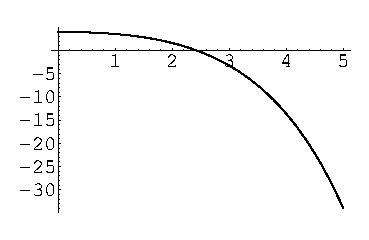
\includegraphics[width=0.3\textwidth]{ode/techniques_linear/6y5yy}
      \end{center}
      \caption{The solution decreases without bound at \textit{t} increases.}
      \label{figure 6y5yy}
    \end{figure}
    %%
    %%
    %%
  \item 
    We consider the problem
    \[
    y'' - 2 y' + 5 y = 0,\quad y(\pi/ 2) = 0,\quad y'(\pi/ 2) = 2.
    \]
    We make the substitution $y = \e^{\lambda x}$ in the differential equation.
    \begin{gather*}
      \lambda^2 - 2 \lambda + 5 = 0 \\
      \lambda = 1 \pm \sqrt{ 1 - 5 } \\
      \lambda = \{ 1 + \imath 2, 1 - \imath 2 \} 
    \end{gather*}
    The general solution of the differential equation is
    \[
    y = c_1 \e^{t} \cos(2 t) + c_2 \e^{t} \sin(2 t).
    \]
    We apply the initial conditions to determine the constants.
    \begin{gather*}
      y(\pi / 2) = 0 \quad \Rightarrow \quad - c_1 \e^{\pi / 2} = 0 \quad \Rightarrow \quad c_1 = 0 \\
      y'(\pi / 2) = 2 \quad \Rightarrow \quad -2 c_2 \e^{\pi / 2} = 2 \quad \Rightarrow \quad c_2 = - \e^{-\pi / 2}
    \end{gather*}
    The solution subject to the initial conditions is
    \[
    \boxed{
      y = - \e^{t-\pi/2} \sin(2 t).
      }
    \]
    The solution is plotted in Figure~\ref{figure y2y5y}.  The solution oscillates
    with an amplitude that tends to $\infty$ as $t \to \infty$.
    \begin{figure}[tb!]
      \begin{center}
        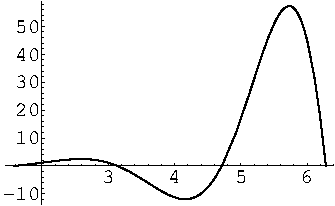
\includegraphics[width=0.3\textwidth]{ode/techniques_linear/y2y5y}
      \end{center}
      \caption{The amplitude of the oscilations increases without bound.}
      \label{figure y2y5y}
    \end{figure}
    %%
    %%
    %%
  \item 
    We consider the problem
    \[
    y'' + 4 y' + 4 y = 0,\quad y(-1) = 2,\quad y'(-1) = 1.
    \]
    We make the substitution $y = \e^{\lambda x}$ in the differential equation.
    \begin{gather*}
      \lambda^2 + 4 \lambda + 4 = 0 \\
      (\lambda + 2)^2 = 0 \\
      \lambda = -2
    \end{gather*}
    The general solution of the differential equation is
    \[
    y = c_1 \e^{-2 t} + c_2 t \e^{-2 t}.
    \]
    We apply the initial conditions to determine the constants.
    \begin{gather*}
      c_1 \e^{2} - c_2 \e^{2} = 2, \quad -2 c_1 \e^{2} + 3 c_2 \e^{2} = 1 \\
      c_1 = 7 \e^{-2}, \quad c_2 = 5 \e^{-2}
    \end{gather*}
    The solution subject to the initial conditions is
    \[
    \boxed{
      y = (7 + 5 t) \e^{-2 (t+1)} 
      }
    \]
    The solution is plotted in Figure~\ref{figure y4y4y}.  The solution vanishes
    as $t \to \infty$.
    \[
    \lim_{t \to \infty} (7 + 5 t) \e^{-2 (t+1)} 
    = \lim_{t \to \infty} \frac{7 + 5 t}{\e^{2 (t+1)}}
    = \lim_{t \to \infty} \frac{5}{2 \e^{2 (t+1)}}
    = 0
    \]
    \begin{figure}[tb!]
      \begin{center}
        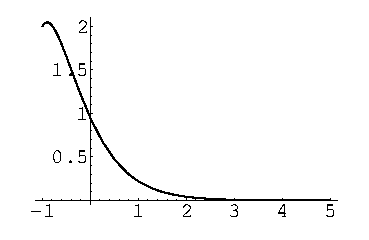
\includegraphics[width=0.3\textwidth]{ode/techniques_linear/y4y4y}
      \end{center}
      \caption{The solution vanishes as \textit{t} increases.}
      \label{figure y4y4y}
    \end{figure}
  \end{enumerate}
\end{Solution}











%% Find two linearly independent solutions to \[ y'' - 4 y' + 13 y = 0.   \]
\begin{Solution}
  \label{solution y-4y+13y}
  \[ 
  y'' - 4 y' + 13 y = 0. 
  \]
  With the substitution $y = \e^{\lambda x}$ we obtain
  \begin{gather*}
    \lambda^2 \e^{\lambda x} - 4 \lambda \e^{\lambda x} + 13 \e^{\lambda x} = 0 \\
    \lambda^2 - 4 \lambda + 13 = 0 \\
    \lambda = 2 \pm 3 i.
  \end{gather*}
  Thus two linearly independent solutions are
  \[ 
  \e^{(2 + 3i)x}, \quad \mathrm{and} \quad \e^{(2-3i)x}. 
  \]
  Noting that
  \begin{align*}
    \e^{(2+3i)x} &= \e^{2x} [\cos (3x) + \imath \sin(3x)] \\
    \e^{(2-3i)x} &= \e^{2x} [\cos (3x) - \imath \sin(3x)],
  \end{align*}
  we can write the two linearly independent solutions
  \[ 
  \boxed{ 
    y_1 = \e^{2x} \cos (3x), \qquad y_2 = \e^{2x} \sin(3x).
    } 
  \]
\end{Solution}






%% Find the general solution to \[ y''' - y'' + y' - y = 0. \]
\begin{Solution}
  \label{solution y-y+y-y=0}
  We note that 
  \[ 
  y''' - y'' + y' - y = 0 
  \]
  is a constant coefficient equation.  The substitution, $y = \e^{\lambda x}$,
  yields
  \begin{gather*}
    \lambda^3 - \lambda^2 + \lambda - 1 = 0 \\
    (\lambda-1)(\lambda-i)(\lambda+i) = 0.
  \end{gather*}
  The corresponding solutions are $\e^x$, $\e^{\imath x}$, and $\e^{-\imath x}$.  We 
  can write the general solution as
  \[ 
  \boxed{
    y = c_1 \e^x + c_2 \cos x + c_3 \sin x. 
    } 
  \]
\end{Solution}



%% Fundamental sets of solutions at $x = 0$ and $x = 1$.
\begin{Solution}
  \label{solution fund set x=0 x=1}
  We start with the equation $y'' + y = 0$.  We substitute $y = \e^{\lambda x}$
  into the differential equation to obtain
  \[
  \lambda^2 + 1 = 0, \qquad \lambda = \pm i.
  \]
  A linearly independent set of solutions is
  \[
  \{ \e^{\imath x}, \e^{-\imath x} \}.
  \]
  The 
  \hyperref[section The Fundamental Set of Solutions]
    {fundamental set of solutions}
  has the form
  \begin{align*}
    y_1 &= c_1 \e^{\imath x} + c_2 \e^{-\imath x}, \\
    y_2 &= c_3 \e^{\imath x} + c_4 \e^{-\imath x}.
  \end{align*}
  By applying the constraints
  \begin{alignat*}{2}
    y_1(0) &= 1, &\quad y_1'(0) &= 0, \\
    y_2(0) &= 0, &\quad y_2'(0) &= 1, 
  \end{alignat*}
  we obtain
  \begin{align*}
    y_1 &= \frac{\e^{\imath x} + \e^{-\imath x}}{2} = \cos x, \\
    y_2 &= \frac{\e^{\imath x} + \e^{-\imath x}}{\imath 2} = \sin x.
  \end{align*}

  Now consider the equation $y'' - y = 0$.  By substituting $y = \e^{\lambda x}$
  we find that a set of solutions is
  \[
  \{ \e^x, \e^{-x} \}.
  \]
  By taking linear combinations of these we see that another set of solutions 
  is
  \[
  \{ \cosh x, \sinh x \}.
  \]
  Note that this is the 
  \hyperref[section The Fundamental Set of Solutions]
    {fundamental set of solutions}.

  Next consider $y'' = 0$.  We can find the solutions by substituting
  $y = \e^{\lambda x}$ or by integrating the equation twice.  The 
  \hyperref[section The Fundamental Set of Solutions]
    {fundamental set of solutions}
  as $x = 0$ is
  \[
  \{ 1, x \}.
  \]

  Note that if $u(x)$ is a solution of a constant coefficient differential 
  equation, then $u(x+c)$ is also a solution.  Also note that if $u(x)$ 
  satisfies $y(0) = a$, $y'(0) = b$, then $u(x-x_0)$ satisfies 
  $y(x_0) = a$, $y'(x_0) = b$.  Thus the 
  \hyperref[section The Fundamental Set of Solutions]
    {fundamental sets of solutions}
  at $x = 1$ are
  \begin{enumerate}
  \item $\{ \cos(x-1), \sin(x-1) \}$,
  \item $\{ \cosh(x-1), \sinh(x-1) \}$,
  \item $\{ 1, x-1 \}$.
  \end{enumerate}
\end{Solution}







%% Damped harmonic motion
\begin{Solution}
  \label{solution damped harmonic motion}
  Let $y(t)$ denote the displacement of the mass from equilibrium.  
  The forces on the mass are $-k y(t)$ due to the spring and $- \mu y'(t)$
  due to friction.  We equate the external forces to $m y''(t)$ to find the
  differential equation of the motion.
  \begin{gather*}
    m y'' = - k y - \mu y' \\
    \boxed{
      y'' + \frac{\mu}{m} y' + \frac{k}{m} y = 0
      }
  \end{gather*}
  The solution which satisfies the initial conditions $y(0) = 0$, $y'(0) = 1$ is
  \[
  \boxed{
    y(t) = 
    \begin{cases}
      \e^{-\mu t / (2 m)} \frac{2 m}{\sqrt{\mu^2- 4 k m}} 
      \sinh \left( \sqrt{\mu^2 - 4 k m}\, t / (2 m) \right)
      \quad &\mathrm{if}\ \mu^2 > k m, \\
      \e^{-\mu t / (2 m)} \frac{2 m}{\sqrt{4 k m - \mu^2}} 
      \sin \left( \sqrt{4 k m - \mu^2}\, t / (2 m) \right)
      \quad &\mathrm{if}\ \mu^2 < k m, \\
      t \e^{-\mu t / (2 m)} 
      \quad &\mathrm{if}\ \mu^2 = k m.
    \end{cases}
    }
  \]
  We respectively call these cases: strongly damped, weakly damped and 
  critically damped.  In the case that $m = k = 1$ the solution is
  \[
  y(t) = 
  \begin{cases}
    \e^{-\mu t / 2} \frac{2}{\sqrt{\mu^2-4}} 
    \sinh \left( \sqrt{\mu^2 - 4}\, t / 2 \right)
    \quad &\mathrm{if}\ \mu > 2, \\
    \e^{-\mu t / 2} \frac{2}{\sqrt{4 - \mu^2}} 
    \sin \left( \sqrt{4 - \mu^2}\, t / 2 \right)
    \quad &\mathrm{if}\ \mu < 2, \\
    t \e^{- t} 
    \quad &\mathrm{if}\ \mu = 2.
  \end{cases}
  \]
  Note that when $t$ is large, $t \e^{-t}$ is much smaller than 
  $\e^{-\mu t / 2}$ for $\mu < 2$.  To prove this we examine the ratio of these
  functions as $t \to \infty$.
  \begin{align*}
    \lim_{t \to \infty} \frac{t \e^{-t}}{\e^{-\mu t / 2}}
    &= \lim_{t \to \infty} \frac{t}{\e^{(1 - \mu / 2) t}} \\
    &= \lim_{t \to \infty} \frac{1}{(1 - \mu / 2) \e^{(1 - \mu) t}} \\
    &= 0
  \end{align*}
  Using this result, we see that the critically damped solution decays faster
  than the weakly damped solution.  

  We can write the strongly damped solution as
  \[
  \e^{-\mu t / 2} \frac{2}{\sqrt{\mu^2-4}} 
  \left( \e^{\sqrt{\mu^2 - 4}\, t / 2} 
    - \e^{-\sqrt{\mu^2 - 4}\, t / 2} \right).
  \]
  For large $t$, the dominant factor is 
  $\e^{\left( \sqrt{\mu^2 - 4} - \mu \right) t / 2}$.  Note that for $\mu > 2$,
  \[
  \sqrt{\mu^2 - 4} = \sqrt{(\mu+2)(\mu-2)} > \mu - 2.
  \]
  Therefore we have the bounds
  \[
  -2 < \sqrt{\mu^2 - 4} - \mu < 0.
  \]
  This shows that the critically damped solution decays faster than the
  strongly damped solution.  $\mu = 2$ gives the fastest decaying solution.
  Figure~\ref{damped} shows the solution for $\mu = 4$, $\mu = 1$ and 
  $\mu = 2$.
  \begin{figure}[tb!]
    \begin{center}
      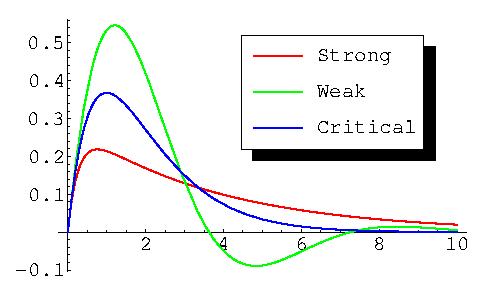
\includegraphics[width=0.4\textwidth]{ode/techniques_linear/damped}
    \end{center}
    \caption{Strongly, weakly and critically damped solutions.}
    \label{damped}
  \end{figure}
\end{Solution}
%% CONTINUE : Check the graph.










%% Show that $y = c \cos(x - \phi)$ is the general solution of 
\begin{Solution}
  \label{solution y=c cos x-phi}
  Clearly $y = c \cos(x - \phi)$ satisfies the differential equation 
  $y'' + y = 0$.  Since it is a two-parameter family of functions, 
  it must be the general solution.

  Using a trigonometric identity we can rewrite the solution as
  \[
  y = c \cos \phi \cos x + c \sin \phi \sin x.
  \]
  Setting this equal to $\sin x$ gives us the two equations
  \begin{align*}
    c \cos \phi &= 0, \\
    c \sin \phi &= 1,
  \end{align*}
  which has the solutions $c = 1$, $\phi = (2 n + 1/2) \pi$, and 
  $c = -1$, $\phi = (2 n - 1/2) \pi$, for $n \in \mathbb{Z}$.

  Clearly $y = c \cosh(x - \phi)$ satisfies the differential equation 
  $y'' - y = 0$.  Since it is a two-parameter family of functions, 
  it must be the general solution.

  Using a trigonometric identity we can rewrite the solution as
  \[
  y = c \cosh \phi \cosh x + c \sinh \phi \sinh x.
  \]
  Setting this equal to $\sinh x$ gives us the two equations
  \begin{align*}
    c \cosh \phi &= 0, \\
    c \sinh \phi &= 1,
  \end{align*}
  which has the solutions $c = -i$, $\phi = \imath (2 n + 1/2) \pi$, and 
  $c = i$, $\phi = \imath (2 n - 1/2) \pi$, for $n \in \mathbb{Z}$.
\end{Solution}







%% \frac{\dd^2 y}{\dd t^2} + 5 \frac{\dd y}{\dd t} + 6 y = 0
\begin{Solution}
  \label{solution y+5y+6y}
  We substitute $y = \e^{\lambda t}$ into the differential equation.
  \begin{gather*}
    \lambda^2 \e^{\lambda t} + 5 \lambda \e^{\lambda t} + 6 \e^{\lambda t} = 0 \\
    \lambda^2 + 5 \lambda + 6 = 0 \\
    (\lambda + 2)(\lambda + 3) = 0
  \end{gather*}
  The general solution of the differential equation is 
  \[
  y = c_1 \e^{-2 t} + c_2 \e^{-3 t}.
  \]
  The initial conditions give us the constraints:
  \begin{gather*}
    c_1 + c_2 = 1, \\
    -2 c_1 - 3 c_2 = V.
  \end{gather*}
  The solution subject to the initial conditions is
  \[
  \boxed{
    y = (3 + V) \e^{-2 t} - (2 + V) \e^{-3 t}.
    }
  \]
  This solution will be non-negative for $t > 0$ if $V \geq -3$.
\end{Solution}






%% y'' + \sign(x) y = 0, \quad -\infty < x < \infty.
\begin{Solution}
  \label{solution y+sign y}
  For negative $x$, the differential equation is
  \[
  y'' - y = 0.
  \]
  We substitute $y = \e^{\lambda x}$ into the differential equation to find
  the solutions.
  \begin{gather*}
    \lambda^2 - 1 = 0 \\
    \lambda = \pm 1 \\
    y = \left\{ \e^x, \e^{-x} \right\} \\
    \intertext{We can take linear combinations to write the solutions in terms of
      the hyperbolic sine and cosine.}
    y = \left\{ \cosh(x), \sinh(x) \right\}
  \end{gather*}

  For positive $x$, the differential equation is
  \[
  y'' + y = 0.
  \]
  We substitute $y = \e^{\lambda x}$ into the differential equation to find
  the solutions.
  \begin{gather*}
    \lambda^2 + 1 = 0 \\
    \lambda = \pm \imath \\
    y = \left\{ \e^{\imath x}, \e^{-\imath x} \right\} \\
    \intertext{We can take linear combinations to write the solutions in terms of
      the sine and cosine.}
    y = \left\{ \cos(x), \sin(x) \right\}
  \end{gather*}

  We will find the 
  \hyperref[section The Fundamental Set of Solutions]
    {fundamental set of solutions}
  at $x = 0$.  That is, we will
  find a set of solutions, $\{y_1, y_2\}$ that satisfy the conditions:
  \begin{alignat*}{2}
    y_1(0) &= 1 &\quad y_1'(0) &= 0 \\
    y_2(0) &= 0 &\quad y_2'(0) &= 1 \\
  \end{alignat*}
  Clearly, these solutions are
  \[
  \boxed{
    y_1 = \begin{cases}
      \cosh(x) &x < 0 \\
      \cos(x) &x \geq 0
    \end{cases}
    \qquad
    y_2 = \begin{cases}
      \sinh(x) &x < 0 \\
      \sin(x) &x \geq 0
    \end{cases}
    }
  \]
\end{Solution}








%%-----------------------------------------------------------------------------
\begin{large}
  \noindent
  \textbf{Euler Equations}
\end{large}








%% x^2 y'' + x y' + y = 0, \qquad x > 0.
\begin{Solution}
  \label{solution x2y+xy+y}
  We consider an Euler equation,
  \[
  x^2 y'' + x y' + y = 0, \quad x > 0.
  \]
  We make the change of independent variable $\xi = \ln x$, $u(\xi) = y(x)$
  to obtain
  \[
  u'' + u = 0.
  \]
  We make the substitution $u(\xi) = \e^{\lambda \xi}$.
  \begin{gather*}
    \lambda^2 + 1 = 0 \\
    \lambda = \pm i
  \end{gather*}
  A set of linearly independent solutions for $u(\xi)$ is
  \[
  \{ \e^{\imath \xi}, \e^{-\imath \xi} \}.
  \]
  Since
  \[
  \cos \xi = \frac{\e^{\imath \xi} + \e^{-\imath \xi} }{2} \quad \mathrm{and} \quad
  \sin \xi = \frac{\e^{\imath \xi} - \e^{-\imath \xi} }{\imath 2},
  \]
  another linearly independent set of solutions is
  \[
  \{ \cos \xi, \sin \xi \}.
  \]
  The general solution for $y(x)$ is
  \[
  \boxed{
    y(x) = c_1 \cos( \ln x ) + c_2 \sin( \ln x ).
    }
  \]
\end{Solution}





%% Find the general solution of \[ x^2 y'' - 2 x y + 2 y = 0.  \]
\begin{Solution}
  \label{solution x2y-2xy+2y}
  Consider the differential equation
  \[ 
  x^2 y'' - 2 x y + 2 y = 0. 
  \]
  With the substitution $y = x^{\lambda}$ this equation becomes
  \begin{gather*}
    \lambda(\lambda-1) - 2 \lambda + 2 = 0 \\
    \lambda^2 - 3 \lambda + 2 = 0 \\
    \lambda = 1, 2.
  \end{gather*}
  The general solution is then
  \[ 
  \boxed{ y = c_1 x + c_2 x^2.} 
  \]
\end{Solution}



%% Find the general solution of \[ x y''' + y'' + \frac{1}{x} y' = 0. \]
\begin{Solution}
  \label{solution xy+y+1xy}
  We note that
  \[ 
  x y''' + y'' + \frac{1}{x} y' = 0 
  \]
  is an Euler equation.  The substitution $y = x^\lambda$ yields
  \begin{gather*}
    \lambda^3 - 3 \lambda^2 + 2 \lambda + \lambda^2 - \lambda + \lambda = 0 \\
    \lambda^3 - 2 \lambda^2 + 2 \lambda = 0.
  \end{gather*}
  The three roots of this algebraic equation are
  \begin{alignat*}{3}
    \lambda &= 0,   &\quad   \lambda &= 1 + i,       &\quad  \lambda &= 1 - \imath \\
    \intertext{The corresponding solutions to the differential equation are}
    y &= x^0        &\quad  y &= x^{1 + \imath}    &\quad  y &= x^{1 - \imath} \\
    y &= 1          &\quad  y &= x \e^{\imath \ln x}      &\quad  y &= x \e^{-\imath \ln x}.
  \end{alignat*}
  We can write the general solution as
  \[ 
  \boxed{ 
    y = c_1 + c_2 x \cos(\ln x) + c_3 \sin(\ln x). 
    } 
  \]
\end{Solution}






%% Find the general solution of \[ x^2 y'' + (2 a + 1) x y' + b y = 0.
\begin{Solution}
  \label{solution x2y+2a1xy+by}
  We substitute $y = x^\lambda$ into the differential equation.
  \begin{gather*}
    x^2 y'' + (2 a + 1) x y' + b y = 0 \\
    \lambda(\lambda - 1) + (2 a + 1) \lambda + b = 0 \\
    \lambda^2 + 2 a \lambda + b  = 0 \\
    \lambda = -a \pm \sqrt{a^2 - b}
  \end{gather*}
  For $a^2 > b$ then the general solution is
  \[
  y = c_1 x^{-a + \sqrt{a^2 - b}} + c_2 x^{-a - \sqrt{a^2 - b}}.
  \]
  For $a^2 < b$, then the general solution is
  \[
  y = c_1 x^{-a + \imath \sqrt{b - a^2}} + c_2 x^{-a - \imath \sqrt{b - a^2}}.
  \]
  By taking the sum and difference of these solutions, we can write the 
  general solution as
  \[
  y = c_1 x^{-a} \cos \left( \sqrt{b - a^2}\, \ln x \right)
  + c_2 x^{-a} \sin \left( \sqrt{b - a^2}\, \ln x \right).
  \]
  For $a^2 = b$, the quadratic in lambda has a double root at $\lambda = a$.
  The general solution of the differential equation is
  \[
  y = c_1 x^{-a} + c_2 x^{-a} \ln x.
  \]
  In summary, the general solution is:
  \[
  \boxed{
    y = 
    \begin{cases}
      x^{-a} \left( c_1 x^{\sqrt{a^2 - b}} 
        + c_2 x^{- \sqrt{a^2 - b}} \right)
      \quad &\mathrm{if}\ a^2 > b, \\
      x^{-a} \left( c_1 \cos \left( \sqrt{b - a^2}\, \ln x \right)  
        + c_2 \sin \left( \sqrt{b - a^2}\, \ln x \right) \right)
      \quad &\mathrm{if}\ a^2 < b, \\
      x^{-a} \left( c_1 + c_2 \ln x \right)
      \quad &\mathrm{if}\ a^2 = b. 
    \end{cases}
    }
  \]
\end{Solution}





%% Solution defined for all values of the parameter.
\begin{Solution}
  \label{solution y1=eax}
  For $a \neq 0$, two linearly independent solutions of
  \[
  y'' - a^2 y = 0
  \]
  are 
  \[
  y_1 = \e^{a x}, \quad y_2 = \e^{-a x}.
  \]
  For $a = 0$, we have
  \[
  y_1 = \e^{0 x} = 1, \quad y_2 = x \e^{0 x} = x.
  \]
  In this case the solution are defined by
  \[
  y_1 = \left[\e^{a x} \right]_{a = 0}, \quad
  y_2 = \left[\frac{\dd}{\dd a} \e^{a x} \right]_{a = 0}.
  \]
  By the definition of differentiation, $f'(0)$ is 
  \[
  f'(0) = \lim_{a \to 0} \frac{f(a) - f(-a)}{2a}.
  \]
  Thus the second solution in the case $a = 0$ is
  \[
  y_2 = \lim_{a \to 0} \frac{\e^{a x} - \e^{-a x}}{a}
  \]
  Consider the solutions
  \[
  y_1 = \e^{a x}, \quad
  y_2 = \lim_{\alpha \to a} \frac{\e^{\alpha x} - \e^{-\alpha x}}{\alpha}.
  \]
  Clearly $y_1$ is a solution for all $a$.  For $a \neq 0$, $y_2$ is a linear
  combination of $\e^{a x}$ and $\e^{-a x}$ and is thus a solution.  
  Since the coefficient of $\e^{-a x}$ in this linear combination is non-zero,
  it is linearly independent to $y_1$.  For $a = 0$, $y_2$ is one half
  the derivative of $\e^{a x}$ evaluated at $a = 0$.  Thus it is a solution.


  For $a \neq 0$, two linearly independent solutions of
  \[
  x^2 y'' + x y' - a^2 y = 0
  \]
  are 
  \[
  y_1 = x^a, \quad y_2 = x^{-a}.
  \]
  For $a = 0$, we have
  \[
  y_1 = \left[ x^a \right]_{a = 0} = 1, \quad 
  y_2 = \left[ \frac{\dd}{\dd a} x^a \right]_{a = 0} = \ln x.
  \]
  Consider the solutions
  \[
  y_1 = x^a, \quad
  y_2 = \frac{x^a - x^{-a}}{a}
  \]
  Clearly $y_1$ is a solution for all $a$.  For $a \neq 0$, $y_2$ is a linear
  combination of $x^a$ and $x^{-a}$ and is thus a solution.  
  For $a = 0$, $y_2$ is one half the derivative of $x^a$ evaluated at $a = 0$.  
  Thus it is a solution.
\end{Solution}








%% Find two linearly independent solutions (i.e., the general solution) of 
\begin{Solution}
  \label{solution x2y-2xy+2y=0}
  \begin{enumerate}
    %%
    %%
    %%
  \item
    \[
    x^2 y'' - 2 x y' + 2 y = 0
    \]
    We substitute $y = x^\lambda$ into the differential equation.
    \begin{gather*}
      \lambda (\lambda - 1) - 2 \lambda + 2 = 0 \\
      \lambda^2 - 3 \lambda + 2 = 0 \\
      (\lambda - 1)(\lambda - 2) = 0 \\
      \boxed{
        y = c_1 x + c_2 x^2
        }
    \end{gather*}
    %%
    %%
    %%
  \item
    \[
    x^2 y'' - 2 y = 0
    \]
    We substitute $y = x^\lambda$ into the differential equation.
    \begin{gather*}
      \lambda (\lambda - 1) - 2 = 0 \\
      \lambda^2 - \lambda - 2 = 0 \\
      (\lambda + 1)(\lambda - 2) = 0 \\
      \boxed{
        y = \frac{c_1}{x} + c_2 x^2
        }
    \end{gather*}
    %%
    %%
    %%
  \item
    \[
    x^2 y'' - x y' + y = 0
    \]
    We substitute $y = x^\lambda$ into the differential equation.
    \begin{gather*}
      \lambda (\lambda - 1) - \lambda + 1 = 0 \\
      \lambda^2 - 2 \lambda + 1 = 0 \\
      (\lambda - 1)^2 = 0 \\
      \intertext{Since there is a double root, the solution is:}
      \boxed{
        y = c_1 x + c_2 x \ln x.
        }
    \end{gather*}
  \end{enumerate}
\end{Solution}







%%-----------------------------------------------------------------------------
\begin{large}
  \noindent
  \textbf{Exact Equations}
\end{large}



%% Solve the differential equation \[ y'' + y' \sin x + y \cos x  = 0. \]
\begin{Solution}
  \label{solution y+ysinx+ycosx}
  We note that
  \[ 
  y'' + y' \sin x + y \cos x = 0 
  \]
  is an exact equation.
  \begin{gather*}
    \frac{\dd}{\dd x} [ y' + y \sin x] = 0 \\
    y' + y \sin x = c_1 \\
    \frac{\dd}{\dd x} \left[ y \e^{-\cos x} \right] = c_1 \e^{-\cos x} \\
    \boxed{ 
      y = c_1 \e^{\cos x} \int \e^{-\cos x}\,\dd x + c_2 \e^{\cos x} 
      }
  \end{gather*}
\end{Solution}



%%-----------------------------------------------------------------------------
\begin{large}
  \noindent
  \textbf{Equations Without Explicit Dependence on \protect$ \mathbf{y} \protect$}
\end{large}

%%-----------------------------------------------------------------------------
\begin{large}
  \noindent
  \textbf{Reduction of Order}
\end{large}





%% (1-x^2) y'' - 2 x y' + 2 y = 0, \quad -1 < x < 1
\begin{Solution}
  \label{solution 1-x2y-2xy+2y}
  \[
  (1-x^2) y'' - 2 x y' + 2 y = 0, \quad -1 < x < 1
  \]
  We substitute $y = x$ into the differential equation to check that it is
  a solution.
  \[
  (1-x^2) (0) - 2 x (1) + 2 x = 0
  \]
  We look for a second solution of the form $y = x u$.  We substitute 
  this into the differential equation and use the fact that $x$ is a solution.
  \begin{gather*}
    (1-x^2) (x u'' + 2 u') - 2 x (x u' + u) + 2 x u = 0 \\
    (1-x^2) (x u'' + 2 u') - 2 x (x u') = 0 \\
    (1-x^2) x u'' + (2 - 4 x^2) u' = 0 \\
    \frac{u''}{u'} = \frac{2 - 4 x^2}{x(x^2 - 1)} \\
    \frac{u''}{u'} = - \frac{2}{x} + \frac{1}{1-x} - \frac{1}{1+x} \\
    \ln(u') = -2 \ln(x) - \ln(1-x) - \ln(1+x) + \mathrm{const} \\
    \ln(u') = \ln \left( \frac{c}{x^2 (1-x)(1+x)} \right) \\
    u' = \frac{c}{x^2 (1-x)(1+x)} \\
    u' = c \left( \frac{1}{x^2} + \frac{1}{2(1-x)} + \frac{1}{2(1+x)} \right) \\
    u = c \left( - \frac{1}{x} - \frac{1}{2} \ln(1-x) + \frac{1}{2} \ln(1+x) 
    \right) + \mathrm{const} \\
    u = c \left( - \frac{1}{x} + \frac{1}{2} \ln \left( \frac{1+x}{1-x} \right)
    \right)
    + \mathrm{const} 
  \end{gather*}
  A second linearly independent solution is
  \[
  \boxed{
    y = - 1 + \frac{x}{2} \ln \left( \frac{1+x}{1-x} \right).
    }
  \]
\end{Solution}







%% Reduction of order where $\e^x$ is one solution.
\begin{Solution}
  \label{solution y-x+1xy+1xy}
  We are given that $y = \e^x$ is a solution of
  \[ 
  y'' - \frac{x + 1}{x} y' + \frac{1}{x} y = 0.
  \]
  To find another linearly independent solution, we will use reduction of 
  order.  Substituting 
  \begin{align*}
    y &= u \e^x \\ 
    y' &= (u' + u)\e^x \\
    y'' &= (u'' + 2u' + u)\e^x
  \end{align*}
  into the differential equation yields
  \begin{gather*}
    u'' + 2u' + u - \frac{x+1}{x} (u' + u) + \frac{1}{x} u = 0. \\
    u'' + \frac{x-1}{x} u' = 0 \\
    \frac{\dd}{\dd x} \left[ u' \exp\left(\int \left(1 - \frac{1}{x}\right)\,\dd x 
      \right) \right] = 0 \\
    u' \e^{x - \ln x} = c_1 \\
    u' = c_1 x \e^{-x} \\
    u = c_1 \int x \e^{-x}\,\dd x + c_2  \\
    u = c_1 (x \e^{-x} + \e^{-x}) + c_2  \\
    y = c_1 (x + 1) + c_2 \e^x  \\
    \intertext{Thus a second linearly independent solution is}
    \boxed{ 
      y = x+1. 
      }
  \end{gather*}
\end{Solution}













%% Reduction of order where $x$ is one solution.
\begin{Solution}
  \label{solution 1-2xy+4xy-4y}
  We are given that $y = x$ is a solution of
  \[ 
  (1 - 2 x) y'' + 4 x y' - 4 y = 0.
  \]
  To find another linearly independent solution, we will use reduction of 
  order.  Substituting 
  \begin{align*}
    y &= x u \\
    y' &= x u' + u \\
    y'' &= x u'' + 2 u'
  \end{align*}
  into the differential equation yields
  \begin{gather*}
    (1 - 2 x) (x u'' + 2 u') + 4 x (x u' + u) - 4 x u = 0, \\
    (1 - 2 x) x u'' + (4 x^2 - 4 x + 2) u' = 0, \\
    \frac{u''}{u'} = \frac{4 x^2 - 4 x + 2}{x (2 x - 1)}, \\
    \frac{u''}{u'} = 2 - \frac{2}{x} + \frac{2}{2 x - 1}, \\
    \ln(u') = 2 x - 2 \ln x + \ln(2 x - 1) + \mathrm{const}, \\
    u' = c_1 \left( \frac{2}{x} - \frac{1}{x^2} \right) \e^{2 x}, \\
    u = c_1 \frac{1}{x} \e^{2 x} + c_2, \\
    \boxed{
      y = c_1 \e^{2 x} + c_2 x.
      }
  \end{gather*}
\end{Solution}






\begin{Solution}
  \label{solution (x-1)y-xy+y=0}
  One solution of
  \[ 
  (x-1) y\prime\prime - x y\prime + y = 0, 
  \]
  is $y_1 = \e^x$.  We find a second solution with reduction of order.  We 
  make the substitution $y_2 = u \e^x$ in the differential equation.
  We determine $u$ up to an additive constant.
  \begin{gather*}
    (x - 1) (u'' + 2 u' + u) \e^x - x (u' + u) \e^x + u \e^x = 0
    \\
    (x - 1) u'' + (x - 2) u' = 0
    \\
    \frac{u''}{u'} = - \frac{x - 2}{x - 1} = -1 + \frac{1}{x - 1}
    \\
    \ln | u' | = - x + \ln |x-1| + c
    \\
    u' = c (x - 1) \e^{-x}
    \\
    u = -c x \e^{-x}
  \end{gather*}
  The second solution of the differential equation is $y_2 = x$.
\end{Solution}







%%-----------------------------------------------------------------------------
\begin{large}
  \noindent
  \textbf{*Reduction of Order and the Adjoint Equation}
\end{large}
















\raggedbottom
}











\flushbottom


%% CONTINUE:
%% Derive the general solution of the Bernoulli equation in an exercise.
%% Show this result in Result.



%%=============================================================================
%%=============================================================================
\chapter{Techniques for Nonlinear Differential Equations}


In mathematics you don't understand things. You just get used to them.

\begin{flushright}
  - Johann von Neumann
\end{flushright}





%%=============================================================================
\section{Bernoulli Equations}
\index{Bernoulli equations}


Sometimes it is possible to solve a nonlinear equation by
making a change of the dependent variable that converts it into a
linear equation.  One of the most important such equations is the
\textit{Bernoulli equation}
\[
\frac{\dd y}{\dd t} + p(t) y = q(t) y^\alpha, \quad \alpha \neq 1.
\]
The change of dependent variable $u = y^{1-\alpha}$ will yield a first order linear
equation for $u$ which when solved will give us an
implicit solution for $y$.  (See Exercise~\ref{exercise t2dydt+2ty-y3=0}.)




\begin{Result}
  The Bernoulli equation $y' + p(t) y = q(t) y^\alpha,\ \alpha \neq 1$ can 
  be transformed to the first order linear equation
  \[
  \frac{\dd u}{\dd t} + (1-\alpha) p(t) u = (1 - \alpha) q(t)
  \]
  with the change of variables $u = y^{1-\alpha}$.
\end{Result}







\begin{Example}
  Consider the Bernoulli equation
  \begin{gather*}
    y' = \frac{2}{x} y + y^2. \\
    \intertext{First we divide by $y^2$.}
    y^{-2}y' = \frac{2}{x} y^{-1} + 1 \\
    \intertext{We make the change of variable $u = y^{-1}$.}
    -u' = \frac{2}{x} u + 1 \\
    u' + \frac{2}{x} u = -1 \\
    \intertext{The integrating factor is 
      $I(x) = \exp(\int \frac{2}{x}\,d x) = x^2$.}
    \frac{d}{d x}(x^2 u) = -x^2 \\
    x^2 u = -\frac{1}{3} x^3 + c \\
    u = -\frac{1}{3} x + \frac{c}{x^2} \\
    y = \left(-\frac{1}{3} x + \frac{c}{x^2} \right)^{-1}
    \intertext{Thus the solution for $y$ is}
    \boxed{
      y = \frac{ 3 x^2 }{ c - x^2 }.
      }
  \end{gather*}
\end{Example}






%%============================================================================
\section{Riccati Equations}
\index{Riccati equations}

\paragraph{Factoring Second Order Operators.}
Consider the second order linear equation
\[L[y] = \left[\frac{\dd^2}{\dd x^2} + p(x) \frac{\dd}{\dd x} + q(x) \right] y = 
y'' + p(x) y' + q(x) y = f(x).\]
If we were able to factor the linear operator $L$ into the form
\begin{equation}
  \label{eqn_factored}
  L = \left[\frac{\dd}{\dd x} + a(x) \right]\left[\frac{\dd}{\dd x} + b(x)\right],
\end{equation}
then we would be able to solve the differential equation.  Factoring
reduces the problem to a system of first order equations.  We start with the
factored equation
\[\left[\frac{\dd}{\dd x} + a(x) \right]\left[\frac{\dd}{\dd x} + b(x)\right] y
= f(x).\]
We set $u = \left[\frac{\dd}{\dd x} + b(x)\right] y$ and solve the problem
\[ \left[\frac{\dd}{\dd x} + a(x) \right] u = f(x).\]
Then to obtain the solution we solve
\[\left[\frac{\dd}{\dd x} + b(x)\right] y = u.\]


\begin{Example}
  Consider the equation
  \[y'' + \left(x - \frac{1}{x}\right)y' + \left(\frac{1}{x^2} - 1\right)y=0.\]
  Let's say by some insight or just random luck we are able to see that 
  this equation can be factored into
  \[ \left[\frac{\dd}{\dd x} + x \right]\left[\frac{\dd}{\dd x} - \frac{1}{x} \right]y=0.\]
  We first solve the equation
  \begin{gather*}
    \left[\frac{\dd}{\dd x} + x \right] u = 0. \\
    u' + x u = 0 \\
    \frac{\dd}{\dd x} \left(\e^{x^2/2} u\right) = 0 \\
    u = c_1 \e^{-x^2/2}
  \end{gather*}
  Then we solve for $y$ with the equation
  \begin{gather*}
    \left[\frac{\dd}{\dd x} - \frac{1}{x} \right]y = u = c_1 \e^{-x^2/2}. \\
    y' - \frac{1}{x} y = c_1 \e^{-x^2/2} \\
    \frac{\dd}{\dd x} \left(x^{-1} y\right) = c_1 x^{-1} \e^{-x^2/2} \\
    \boxed{y = c_1 x \int x^{-1} \e^{-x^2/2}\,d x + c_2 x}
  \end{gather*}
\end{Example}


If we were able to solve for $a$ and $b$ 
in Equation~\ref{eqn_factored} in terms of $p$ and $q$
then we would be able to solve any second order differential equation.  
Equating the two operators, 
\begin{align*}
  \frac{\dd^2}{\dd x^2} + p \frac{\dd}{\dd x} + q 
  &= \left[\frac{\dd}{\dd x} + a \right]
  \left[\frac{\dd}{\dd x} + b\right] \\
  &= \frac{\dd^2}{\dd x^2} + (a + b)\frac{\dd}{\dd x} 
  + (b' + a b).
\end{align*}
Thus we have the two equations
\[ a + b = p, \quad \mathrm{and} \quad 
b' + a b = q. \]
Eliminating $a$, 
\begin{gather*}
  b' + (p - b) b = q \\
  b' = b^2 - p b + q
\end{gather*}
Now we have a nonlinear equation for $b$ 
that is no easier to solve than the original
second order linear equation.

\paragraph{Riccati Equations.}
Equations of the form
\[ y' = a(x) y^2 + b(x) y + c(x)\]
are called Riccati equations.  From the above derivation we see that for
every second order differential equation there is a corresponding Riccati
equation.  Now we will show that the converse is true.

We make the substitution 
\[y = -\frac{u'}{au}, \qquad 
y' = -\frac{u''}{a u} + \frac{(u')^2}{a u^2} 
+ \frac{a' u'}{a^2 u}, \]
in the Riccati equation.
\begin{gather*}
  y' = a y^2 + b y + c \\
  -\frac{u''}{a u} + \frac{(u')^2}{a u^2} 
  + \frac{a' u'}{a^2 u}
  = a \frac{(u')^2}{a^2 u^2} - b \frac{u'}{a u}+c\\
  -\frac{u''}{a u} + \frac{a' u'}{a^2 u} + b \frac{u'}{a u}
  - c = 0 \\
  u'' - \left(\frac{a'}{a} + b\right) u'+ a c u = 0
\end{gather*}
Now we have a second order linear equation for $u$.



\begin{Result}
  The substitution $y = -\frac{u'}{a u}$ transforms the Riccati 
  equation
  \[
  y' = a(x) y^2 + b(x) y + c(x)
  \]
  into the second order linear equation
  \[
  u'' - \left(\frac{a'}{a} + b\right) u'+ a c u = 0.
  \]
\end{Result}




\begin{Example}
  Consider the Riccati equation
  \[ y' = y^2 + \frac{1}{x} y + \frac{1}{x^2}. \]
  With the substitution $y = -\frac{u'}{u}$ we obtain
  \[ u'' - \frac{1}{x} u' + \frac{1}{x^2} u = 0. \]
  This is an Euler equation.  The substitution $u = x^\lambda$ yields
  \[ \lambda(\lambda-1) - \lambda + 1 = (\lambda-1)^2 = 0. \]
  Thus the general solution for $u$ is
  \[ u = c_1 x + c_2 x \log x. \]
  Since $y = -\frac{u'}{u}$,
  \begin{gather*} 
    y = -\frac{c_1 + c_2 (1 + \log x)}{c_1 x + c_2 x \log x} \\
    \boxed{
      y = -\frac{1 + c (1 + \log x)}{x + c x \log x} 
      }
  \end{gather*}
\end{Example}









%%============================================================================
\section{Exchanging the Dependent and Independent Variables}
\index{exchanging dep. and indep. var.}



Some differential equations can be put in a more elementary form by
exchanging the dependent and independent variables.  If the new equation can
be solved, you will have an implicit solution for the initial
equation. We will consider a few
examples to illustrate the method.




\begin{Example}
  Consider the equation
  \[ y' = \frac{1}{y^3 - x y^2}.\]
  Instead of considering $y$ to be a function of $x$,
  consider $x$ to be a function
  of $y$.  That is, $x = x(y)$, $x' = \frac{\dd x}{\dd y}$.
  \begin{gather*}
    \frac{\dd y}{\dd x} = \frac{1}{y^3 - x y^2} \\
    \frac{\dd x}{\dd y} = y^3 - x y^2 \\
    x' + y^2 x = y^3 \\
    \intertext{Now we have a first order equation for $x$.}
    \frac{\dd}{\dd y} \left(\e^{y^3/3} x\right) = y^3 \e^{y^3/3} \\
    \boxed{x = \e^{-y^3/3} \int y^3 \e^{y^3/3}\,d y + c \e^{-y^3/3}}
  \end{gather*}
\end{Example}


\begin{Example}
  Consider the equation
  \[y' = \frac{y}{y^2 + 2x}.\]
  Interchanging the dependent and independent variables yields
  \begin{gather*}
    \frac{1}{x'} = \frac{y}{y^2 + 2x} \\
    x' = y + 2\frac{x}{y} \\
    x' - 2 \frac{x}{y} = y \\
    \frac{\dd}{\dd y} (y^{-2} x) = y^{-1} \\
    y^{-2} x = \log y + c \\
    \boxed{x = y^2 \log y + c y^2}
  \end{gather*}
\end{Example}





\begin{Result}
  Some differential equations can be put in a simpler form by exchanging
  the dependent and independent variables.  Thus a differential equation for
  $y(x)$ can be written as an equation for $x(y)$.  Solving the equation
  for $x(y)$ will give an implicit solution for $y(x)$.
\end{Result}











%%============================================================================
\section{Autonomous Equations}
\index{differential equations!autonomous}
\index{autonomous D.E.}
Autonomous equations have no explicit dependence on $x$.
The following are examples.
\begin{itemize}
\item $y'' + 3 y' - 2y = 0$
\item $y'' = y + (y')^2$
\item $y''' + y'' y = 0$
\end{itemize}

The change of variables $u(y) = y'$ reduces an $n^{th}$ order
autonomous equation in $y$
to a non-autonomous equation of order $n-1$ in $u(y)$.  Writing the derivatives
of $y$ in terms of $u$,
\begin{align*}
  y'      &= u(y) \\
  y''     &= \frac{\dd}{\dd x} u(y) \\
  &= \frac{\dd y}{\dd x}\frac{\dd}{\dd y} u(y) \\
  &= y' u' \\
  &= u' u \\
  y'''    &= (u'' u + (u')^2)u.
\end{align*}
Thus we see that the equation for $u(y)$ will have an order of one less than
the original equation.



\begin{Result}
  Consider an autonomous differential equation for $y(x)$, 
  (autonomous equations have no explicit dependence on $x$.)
  The change of variables $u(y) = y'$ reduces an $n^{th}$ order
  autonomous equation in $y$
  to a non-autonomous equation of order $n-1$ in $u(y)$.
\end{Result}




\begin{Example}
  Consider the equation
  \[ y'' = y + (y')^2.\]
  With the substitution $u(y) = y'$, the equation becomes
  \begin{gather*}
    u' u = y + u^2 \\
    u' = u + y u^{-1}. \\
    \intertext{We recognize this as a Bernoulli equation.  
      The substitution $v = u^2$ yields}
    \frac{1}{2} v' = v + y \\
    v' - 2v = 2y \\
    \frac{\dd}{\dd y} \left(\e^{-2y} v\right) = 2y \e^{-2y} \\
    v(y) = c_1 \e^{2y} + \e^{2y}\int 2y \e^{-2y}\,d y \\
    v(y) = c_1 \e^{2y} + \e^{2y}\left( -y \e^{-2y} + 
      \int \e^{-2y}\,d y \right) \\
    v(y) = c_1 \e^{2y} + \e^{2y}\left( -y \e^{-2y} - \frac{1}{2} \e^{-2y}\right)\\
    v(y) = c_1 \e^{2y} - y - \frac{1}{2}. \\
    \intertext{Now we solve for $u$.}
    u(y) = \left(c_1 \e^{2y} - y - \frac{1}{2}\right)^{1/2}. \\
    \frac{\dd y}{\dd x} = \left(c_1 \e^{2y} - y - \frac{1}{2}\right)^{1/2} \\
    \intertext{This equation is separable.}
    d x = \frac{d y}{\left(c_1 \e^{2y} - y - \frac{1}{2}\right)^{1/2}} \\
    \boxed{ x + c_2 = \int \frac{1}{\left(c_1 \e^{2y} - y - \frac{1}{2}
        \right)^{1/2}}\,d y }
  \end{gather*}
  Thus we finally have arrived at an implicit solution for $y(x)$.
\end{Example}




\begin{Example}
  Consider the equation
  \[y'' + y^3 = 0.\]
  With the change of variables, $u(y) = y'$, the equation becomes
  \[ u' u + y^3 = 0. \]
  This equation is separable.
  \begin{gather*}
    u\,d u = - y^3\,d y \\
    \frac{1}{2} u^2 = - \frac{1}{4} y^4 + c_1 \\
    u = \left( 2c_1 -\frac{1}{2} y^4 \right)^{1/2} \\
    y' = \left( 2c_1 -\frac{1}{2} y^4 \right)^{1/2} \\
    \frac{d y}{(2c_1 -\frac{1}{2} y^4 )^{1/2}} = d x \\
    \intertext{Integrating gives us the implicit solution}
    \boxed{ \int \frac{1}{(2c_1 -\frac{1}{2} y^4 )^{1/2}}\,d y = x + c_2 .}
  \end{gather*}
\end{Example}













%%============================================================================
\section{*Equidimensional-in-x Equations}
\index{differential equations!equidimensional-in-x}
\index{equidimensional-in-x D.E.} 

Differential equations that are invariant under the change of variables
$x = c\,\xi$
are said to be equidimensional-in-$x$.  
For a familiar example from linear equations, we note that 
the Euler equation is 
equidimensional-in-$x$.  Writing the new derivatives under the change of 
variables,
\[ x = c\,\xi, \qquad \frac{\dd}{\dd x} = \frac{1}{c} \frac{\dd}{\dd \xi}, \qquad
\frac{\dd^2}{\dd x^2} = \frac{1}{c^2}\frac{\dd^2}{\dd \xi^2}, \qquad \ldots.\]




\begin{Example}
  Consider the Euler equation
  \[ y'' + \frac{2}{x} y' + \frac{3}{x^2}y = 0.\]
  Under the change of variables, $x = c\,\xi$, $y(x) = u(\xi)$,
  this equation becomes
  \begin{gather*}
    \frac{1}{c^2} u'' + \frac{2}{c\,\xi} \frac{1}{c}u'
    + \frac{3}{c^2\,\xi^2} u = 0 \\
    u'' + \frac{2}{\xi} u' + \frac{3}{\xi^2}u = 0.
  \end{gather*}
  Thus this equation is invariant under the change of variables $x = c\,\xi$.
\end{Example}



\begin{Example} \label{nonlin_equidim}
  For a nonlinear example, consider the equation
  \[ y''\,y' + \frac{y''}{x\,y}+ \frac{y'}{x^2} = 0.\]
  With the change of variables $x = c\,\xi$, $y(x) = u(\xi)$
  the equation becomes
  \begin{gather*}
    \frac{u''}{c^2}\frac{u'}{c} + \frac{u''}{c^3\,\xi\,u} 
    + \frac{u'}{c^3\,\xi^2} = 0 \\
    u''\,u' + \frac{u''}{\xi\,u} 
    + \frac{u'}{\xi^2} = 0.
  \end{gather*}
  We see that this equation is also equidimensional-in-$x$.
\end{Example}




You may recall that the change of variables $x = \e^t$ reduces an Euler
equation to a constant coefficient equation. 
To generalize this result to nonlinear equations we will see that the
same change of variables reduces an equidimensional-in-$x$ equation to
an autonomous equation.

Writing the derivatives with respect to $x$ in terms of $t$,
\[
x = \e^t, \qquad
\frac{\dd}{\dd x} = \frac{\dd t}{\dd x} \frac{\dd}{\dd t} = \e^{-t}\frac{\dd}{\dd t} 
\]
\[
x\frac{\dd}{\dd x} = \frac{\dd}{\dd t}
\]
\[
x^2 \frac{\dd^2}{\dd x^2} = x \frac{\dd}{\dd x} \left(x \frac{\dd}{\dd x}\right) 
- x\frac{\dd}{\dd x} = \frac{\dd^2}{\dd t^2} - \frac{\dd}{\dd t}.
\]


\begin{Example} 
  Consider the equation in Example~\ref{nonlin_equidim} 
  \[ y''\,y' + \frac{y''}{x\,y}+ \frac{y'}{x^2} = 0.\]
  Applying the change of variables $x = \e^t$, $y(x) = u(t)$ yields an 
  autonomous equation for $u(t)$.
  \begin{gather*}
    x^2\,y''\,x\,y' + \frac{x^2\,y''}{y} + x\,y' = 0 \\
    \boxed{ (u'' - u') u' + \frac{u'' - u'}{u} + u' = 0  }
  \end{gather*}
\end{Example}







\begin{Result}
  A differential equation that is invariant under the change of variables
  $x = c\,\xi$ is equidimensional-in-$x$.  Such an equation can be reduced
  to autonomous equation of the same order with the change of variables,
  $x = \e^t$.
\end{Result}














%%============================================================================
\section{*Equidimensional-in-y Equations}
\index{differential equations!equidimensional-in-y}
\index{equidimensional-in-y D.E.}
A differential equation is said to be equidimensional-in-$y$ if it is invariant
under the change of variables $y(x) = c\,v(x)$.  Note that all linear
homogeneous equations are equidimensional-in-$y$.





\begin{Example} \label{lin_eiy} 
  Consider the linear equation
  \[ y'' + p(x) y' + q(x) y = 0.\]
  With the change of variables $y(x) = c v(x)$ the equation becomes
  \begin{gather*}
    c v'' + p(x)c v' + q(x) c v = 0 \\
    v'' + p(x)v' + q(x) v = 0
  \end{gather*}
  Thus we see that the equation is invariant under the change of variables.
\end{Example}








\begin{Example} \label{nonlin_eiy}
  For a nonlinear example, consider the equation
  \[ y'' y + (y')^2 - y^2 = 0.\]
  Under the change of variables $y(x) = c v(x)$ the equation becomes.
  \begin{gather*}
    c v'' c v + (c v')^2 - (c v)^2 = 0 \\
    v'' v + (v')^2 - v^2 = 0.
  \end{gather*}
  Thus we see that this equation is also equidimensional-in-$y$.
\end{Example}



The change of variables $y(x) = \e^{u(x)}$ reduces an $n^{t h}$ order
equidimensional-in-$y$ equation to an equation of order $n-1$ for $u'$.
Writing the derivatives of $\e^{u(x)}$,
\begin{align*}
  \frac{\dd}{\dd x} \e^u &= u' \e^u \\
  \frac{\dd^2}{\dd x^2} \e^u &= (u'' + (u')^2)\e^u \\
  \frac{d^3}{d x^3}\e^u &= (u''' + 3u'' u'' + (u')^3)\e^u.
\end{align*}


\begin{Example}
  Consider the linear equation in Example~\ref{lin_eiy} 
  \[ y'' + p(x) y' + q(x) y = 0.\]
  Under the change of variables $y(x) = \e^{u(x)}$ the equation becomes
  \begin{gather*}
    (u'' + (u')^2)\e^u + p(x) u' \e^u + q(x) \e^u = 0 \\
    \boxed{ u'' + (u')^2 + p(x) u' + q(x) = 0. }
  \end{gather*}
  Thus we have a Riccati  equation for $u'$.  
  This transformation might seem rather useless since linear equations are usually
  easier to work with than nonlinear equations, but it is often useful in determining
  the asymptotic behavior of the equation.
\end{Example}





\begin{Example}
  From Example~\ref{nonlin_eiy} we have the equation
  \[ y'' y + (y')^2 - y^2 = 0.\]
  The change of variables $y(x) = \e^{u(x)}$ yields
  \begin{gather*}
    (u'' + (u')^2) \e^u \e^u + (u' \e^u)^2 - (\e^u)^2 = 0 \\
    u'' + 2(u')^2 - 1 = 0 \\
    u'' = -2 (u')^2 + 1 
  \end{gather*}
  Now we have a Riccati equation for $u'$.  
  We make the substitution $u' = \frac{v'}{2 v}$.
  \begin{gather*}
    \frac{v''}{2v} - \frac{(v')^2}{2v^2} = - 2 \frac{(v')^2}{4v^2} + 1 \\
    v'' - 2 v = 0 \\
    v = c_1 \e^{\sqrt{2} x} + c_2 \e^{-\sqrt{2} x} \\
    u' = 2 \sqrt{2} \frac{c_1 \e^{\sqrt{2} x} - c_2 \e^{-\sqrt{2} x}}
    {c_1 \e^{\sqrt{2} x} + c_2 \e^{-\sqrt{2} x}} \\
    u = 2 \int \frac{c_1 \sqrt{2} \e^{\sqrt{2} x} 
      - c_2 \sqrt{2} \e^{-\sqrt{2} x}}
    {c_1 \e^{\sqrt{2} x} + c_2 \e^{-\sqrt{2} x}} \,d x + c_3 \\
    u = 2 \log \left( c_1 \e^{\sqrt{2} x} + c_2 \e^{-\sqrt{2} x} \right) + c_3 \\
    y = \left( c_1 \e^{\sqrt{2} x} + c_2 \e^{-\sqrt{2} x} \right)^2 \e^{c_3}
  \end{gather*}
  The constants are redundant, the general solution is
  \[
  \boxed{
    y = \left( c_1 \e^{\sqrt{2} x} + c_2 \e^{-\sqrt{2} x} \right)^2
    }
  \]
\end{Example}




\begin{Result}
  A differential equation is equidimensional-in-$y$ if it is invariant under 
  the change of variables $y(x) = c v(x)$.  An $n^{t h}$ order 
  equidimensional-in-$y$ equation can be reduced to an equation of order 
  $n-1$ in $u'$ with the change of variables $y(x) = \e^{u(x)}$.
\end{Result}











%%============================================================================
\section{*Scale-Invariant Equations}
\index{differential equations!scale-invariant}
\index{scale-invariant D.E.}



\begin{Result}
  An equation is scale invariant if it is invariant under the change of 
  variables, $x = c\xi$, $y(x) = c^\alpha v(\xi)$, for some value of $\alpha$.
  A scale-invariant equation can be transformed to an equidimensional-in-$x$
  equation with the change of variables, $y(x) = x^\alpha u(x)$.
\end{Result}







\begin{Example}
  Consider the equation
  \[ y'' + x^2 y^2 = 0.\]
  Under the change of variables $x = c\xi$, $y(x) = c^\alpha v(\xi)$ this
  equation becomes
  \[ \frac{c^\alpha}{c^2}v''(\xi) + c^2 x^2 c^{2\alpha} v^2(\xi) = 0.\]
  Equating powers of $c$ in the two terms yields $\alpha = -4$.  

  Introducing the change of variables $y(x) = x^{-4}u(x)$ yields
  \begin{gather*}
    \frac{\dd^2}{\dd x^2} \big[ x^{-4}u(x) \big] + x^2 (x^{-4}u(x))^2 = 0 \\
    x^{-4}u'' - 8 x^{-5}u' + 20 x^{-6}u + x^{-6}u^2 = 0 \\
    \boxed{ x^2 u'' - 8 x u' + 20 u + u^2 = 0. }
  \end{gather*}
  We see that the equation for $u$ is equidimensional-in-$x$.
\end{Example}











\raggedbottom
%%==========================================================================
\exercises{
\pagebreak
\flushbottom
\section{Exercises}






%% CONTINUE: add a Clairaut section.
%% y = x p + p^2.
\begin{Exercise}
  \label{exercise y=xp+p2}
  \begin{enumerate}
  \item
    Find the general solution and the singular solution of the Clairaut equation,
    \[
    y = x p + p^2.
    \]
  \item
    Show that the singular solution is the envelope of the general solution.
  \end{enumerate}

  \hintsolution{y=xp+p2}
\end{Exercise}





%%-----------------------------------------------------------------------------
\begin{large}
  \noindent
  \textbf{Bernoulli Equations}
\end{large}






%% \frac{\dd y}{\dd t} + p(t) y = q(t) y^\alpha.
\begin{Exercise}[mathematica/ode/techniques\_nonlinear/bernoulli.nb]
  \label{exercise dydt+py=qy}
  Consider the Bernoulli equation
  \[
  \frac{\dd y}{\dd t} + p(t) y = q(t) y^\alpha.
  \]
  \begin{enumerate}
  \item
    Solve the Bernoulli equation for $\alpha = 1$.
  \item
    Show that for $\alpha \neq 1$ the substitution $u = y^{1-\alpha}$ reduces 
    Bernoulli's equation to a linear equation.
  \item
    Find the general solution to the following equations.
    \begin{enumerate}
    \item 
      \centerline{$\displaystyle t^2 \frac{\dd y}{\dd t} + 2 t y - y^3 = 0,\ t > 0$}
    \item 
      \centerline{$\displaystyle \frac{\dd y}{\dd x} + 2 x y + y^2 = 0$}
    \end{enumerate}
  \end{enumerate}

  \hintsolution{dydt+py=qy}
\end{Exercise}





%% Consider a population, $y$.  Let the birth rate of the population be 
\begin{Exercise}
  \label{exercise population}
  Consider a population, $y$.  Let the birth rate of the population be 
  proportional to $y$ with constant of proportionality $1$.  Let the death
  rate of the population be proportional to $y^2$ with constant of 
  proportionality $1/1000$.  Assume that the population is large enough
  so that you can consider $y$ to be continuous.  What is the population as
  a function of time if the initial population is $y_0$?

  \hintsolution{population}
\end{Exercise}




%% t^2 \frac{\dd y}{\dd t} + 2 t y - y^3 = 0 \quad t > 0
\begin{Exercise}
  \label{exercise t2dydt+2ty-y3=0}
  Show that the transformation $u = y^{1-n}$
  reduces the equation to a linear first order equation.  Solve the equations
  \begin{enumerate}
  \item
    $
    \displaystyle
    t^2 \frac{\dd y}{\dd t} + 2 t y - y^3 = 0 \quad t > 0
    $
  \item
    $
    \displaystyle
    \frac{\dd y}{\dd t} = \left( \Gamma \cos t + T \right) y - y^3,
    $
    $\Gamma$ and $T$ are real constants.  (From a fluid flow stability problem.)
  \end{enumerate}

  \hintsolution{t2dydt+2ty-y3=0}
\end{Exercise}





%%-----------------------------------------------------------------------------
\begin{large}
  \noindent
  \textbf{Riccati Equations}
\end{large}






%% Riccati equations, two methods of solution.
\begin{Exercise}
  \label{exercise riccati 2 methods}
  \begin{enumerate}
    %%
    %%
  \item
    Consider the Ricatti equation,
    \[
    \frac{\dd y}{\dd x} = a(x) y^2 + b(x) y + c(x).
    \]
    Substitute 
    \[
    y = y_p(x) + \frac{1}{u(x)}
    \]
    into the Ricatti equation, where $y_p$ is some particular solution to obtain
    a first order linear differential equation for $u$.
    %%
    %%
  \item
    Consider a Ricatti equation,
    \[
    y' = 1 + x^2 - 2 x y + y^2.
    \]
    Verify that $y_p(x) = x$ is a particular solution.
    Make the substitution $y = y_p + 1/u$ to find the general solution.

    What would happen if you continued this method, taking the general solution
    for $y_p$?  Would you be able to find a more general solution?
    %%
    %%
  \item
    The substitution
    \[
    y = - \frac{u'}{a u}
    \]
    gives us the second order, linear, homogeneous differential equation,
    \[
    u'' - \left( \frac{a'}{a} + b \right) u' + a c u = 0.
    \]
    The general solution for $u$ has two constants of integration.  However, the 
    solution for $y$ should only have one constant of integration as it satisfies
    a first order equation.  Write $y$ in terms of the solution for $u$ and verify
    tha $y$ has only one constant of integration.
  \end{enumerate}

  \hintsolution{riccati 2 methods}
\end{Exercise}






%%-----------------------------------------------------------------------------
\begin{large}
  \noindent
  \textbf{Exchanging the Dependent and Independent Variables}
\end{large}













%% Solve the differential equation \[ y' = \frac{\sqrt{y}}{x y + y}.\]
\begin{Exercise}
  \label{exercise y'=sqrt y xyy}
  Solve the differential equation
  \[
  y' = \frac{\sqrt{y}}{x y + y}.
  \]

  \hintsolution{y'=sqrt y xyy}
\end{Exercise}



%%-----------------------------------------------------------------------------
\begin{large}
  \noindent
  \textbf{Autonomous Equations}
\end{large}



%%-----------------------------------------------------------------------------
\begin{large}
  \noindent
  \textbf{*Equidimensional-in-$\mathbf{x}$ Equations}
\end{large}



%%-----------------------------------------------------------------------------
\begin{large}
  \noindent
  \textbf{*Equidimensional-in-$\mathbf{y}$ Equations}
\end{large}



%%-----------------------------------------------------------------------------
\begin{large}
  \noindent
  \textbf{*Scale-Invariant Equations}
\end{large}







\raggedbottom
}
%%==========================================================================
\hints{
\pagebreak
\flushbottom
\section{Hints}





%% y = x p + p^2.
\begin{Hint}
  \label{hint y=xp+p2}
  %% CONTINUE
\end{Hint}






%%-----------------------------------------------------------------------------
\begin{large}
  \noindent
  \textbf{Bernoulli Equations}
\end{large}





%% \frac{\dd y}{\dd t} + p(t) y = q(t) y^\alpha.
\begin{Hint}
  \label{hint dydt+py=qy}
  %% CONTINUE
\end{Hint}





%% Consider a population, $y$.  Let the birth rate of the population be 
\begin{Hint}
  \label{hint population}
  The differential equation governing the population is
  \[ 
  \frac{\dd y}{\dd t} = y - \frac{y^2}{1000}, \quad y(0) = y_0. 
  \]
  This is a Bernoulli equation.
\end{Hint}





%% t^2 \frac{\dd y}{\dd t} + 2 t y - y^3 = 0 \quad t > 0
\begin{Hint}
  \label{hint t2dydt+2ty-y3=0}
  %% CONTINUE
\end{Hint}



%%-----------------------------------------------------------------------------
\begin{large}
  \noindent
  \textbf{Riccati Equations}
\end{large}





%% Riccati equations, two methods of solution.
\begin{Hint}
  \label{hint riccati 2 methods}
  %% CONTINUE
\end{Hint}







%%-----------------------------------------------------------------------------
\begin{large}
  \noindent
  \textbf{Exchanging the Dependent and Independent Variables}
\end{large}



%% Solve the differential equation \[ y' = \frac{\sqrt{y}}{x y + y}.\]
\begin{Hint}
  \label{hint y'=sqrt y xyy}
  Exchange the dependent and independent variables.
\end{Hint}



%%-----------------------------------------------------------------------------
\begin{large}
  \noindent
  \textbf{Autonomous Equations}
\end{large}



%%-----------------------------------------------------------------------------
\begin{large}
  \noindent
  \textbf{*Equidimensional-in-$\mathbf{x}$ Equations}
\end{large}



%%-----------------------------------------------------------------------------
\begin{large}
  \noindent
  \textbf{*Equidimensional-in-$\mathbf{y}$ Equations}
\end{large}



%%-----------------------------------------------------------------------------
\begin{large}
  \noindent
  \textbf{*Scale-Invariant Equations}
\end{large}








\raggedbottom
}
%%===========================================================================
\solutions{
\pagebreak
\flushbottom
\section{Solutions}







%% y = x p + p^2.
\begin{Solution}
  \label{solution y=xp+p2}
  We consider the Clairaut equation,
  \begin{equation}
    \label{a_clairaut_eqn}
    y = x p + p^2.
  \end{equation}

  \begin{enumerate}
    %%
    %%
  \item
    We differentiate Equation~\ref{a_clairaut_eqn} with respect to $x$ to obtain
    a second order differential equation.
    \begin{gather*}
      y' = y' + x y'' + 2 y' y'' \\
      y'' (2y' + x) = 0
    \end{gather*}
    Equating the first or second factor to zero will lead us to two distinct
    solutions.
    \[
    y'' = 0 \quad \mathrm{or} \quad y' = - \frac{x}{2}
    \]
    If $y'' = 0$ then $y' \equiv p$ is a constant, (say $y' = c$).  From 
    Equation~\ref{a_clairaut_eqn} we see that the general solution is,
    \begin{equation}
      \label{clairaut_first_soln}
      \boxed{
        y(x)  = c x + c^2.
        }
    \end{equation}
    Recall that the general solution of a first order differential equation 
    has one constant of integration.

    If $y' = - x / 2$ then $y = -x^2 / 4 + \mathrm{const}$.  We determine the 
    constant by substituting the expression into Equation~\ref{a_clairaut_eqn}.
    \[
    - \frac{x^2}{4} + c = x \left( - \frac{x}{2} \right) + \left( - \frac{x}{2} 
    \right)^2
    \]
    Thus we see that a singular solution of the Clairaut equation is
    \begin{equation}
      \label{clairaut_second_soln}
      \boxed{
        y(x) = - \frac{1}{4} x^2.
        }
    \end{equation}
    Recall that a singular solution of a first order nonlinear differential 
    equation has no constant of integration.
    %%
    %%
  \item
    Equating the general and singular solutions, $y(x)$, and their derivatives, 
    $y'(x)$, gives us the system of equations,
    \[
    c x + c^2 = - \frac{1}{4} x^2, \qquad c = - \frac{1}{2} x.
    \]
    Since the first equation is satisfied for $c = - x / 2$, we see that 
    the solution $y = c x + c^2$ is tangent to the solution $y = - x^2 / 4$
    at the point $(-2 c, -|c|)$.
    The solution $y = c x + c^2$ is plotted for $c = \ldots,-1/4,0,1/4,\ldots$
    in Figure~\ref{clairaut_envelope}.

    \begin{figure}[tb!]
      \begin{center}
        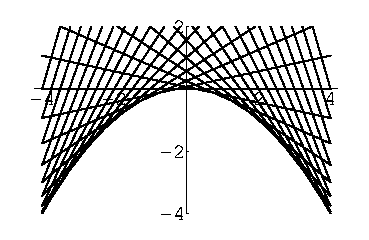
\includegraphics[width=0.4\textwidth]{ode/techniques_nonlinear/clairaut_envelope}
      \end{center}
      \caption{The solutions and their envelope.}
      \label{clairaut_envelope}
    \end{figure}

    The envelope of a one-parameter family $F(x,y,c) = 0$ is given by the 
    system of equations,
    \[
    F(x,y,c) = 0, \qquad F_c(x,y,c) = 0.
    \]
    For the family of solutions $y = c x + c^2$ these equations are
    \[
    y = c x + c^2, \qquad 0 = x + 2 c.
    \]
    Substituting the solution of the second equation, $c = - x/2$, into the
    first equation gives the envelope,
    \[
    y = \left( - \frac{1}{2} x \right) x + \left( - \frac{1}{2} x \right)^2
    = - \frac{1}{4} x^2.
    \]
    Thus we see that the singular solution is the envelope of the general solution.
  \end{enumerate}
\end{Solution}







%%-----------------------------------------------------------------------------
\begin{large}
  \noindent
  \textbf{Bernoulli Equations}
\end{large}







%% \frac{\dd y}{\dd t} + p(t) y = q(t) y^\alpha.
\begin{Solution}
  \label{solution dydt+py=qy}
  \begin{enumerate}
    %%
    %%
  \item
    \begin{gather*}
      \frac{\dd y}{\dd t} + p(t) y = q(t) y \\
      \frac{\dd y}{ y } = (q - p) \,\dd t \\
      \ln y = \int(q - p) \,\dd t + c \\
      \boxed{
        y = c \e^{\int (q - p) \,\dd t}
        }
    \end{gather*}
    %%
    %%
  \item
    We consider the Bernoulli equation,
    \[
    \frac{\dd y}{\dd t} + p(t) y = q(t) y^\alpha, \quad \alpha \neq 1.
    \]
    We divide by $y^\alpha$.
    \[ 
    y^{-\alpha} y' + p(t) y^{1-\alpha} = q(t) 
    \]
    This suggests the change of dependent variable $u = y^{1-\alpha}$,
    $u' = (1-\alpha)y^{-\alpha} y'$.
    \begin{gather*}
      \frac{1}{1-\alpha} \frac{\dd}{\dd t} y^{1-\alpha} + p(t) y^{1-\alpha} = q(t) \\
      \frac{\dd u}{\dd t} + (1-\alpha) p(t) u = (1 - \alpha) q(t)
    \end{gather*}
    Thus we obtain a linear equation for $u$ which when solved will give us an
    implicit solution for $y$.
    %%
    %%
  \item
    \begin{enumerate}
    \item
      \begin{gather*}
        t^2 \frac{\dd y}{\dd t} + 2 t y - y^3 = 0, \quad t > 0 \\
        t^2 \frac{ y' }{ y^3 } + 2 t \frac{ 1 }{ y^2 } = 1
      \end{gather*}
      We make the change of variables $u = y^{-2}$.
      \begin{gather*}
        - \frac{1}{2} t^2 u' + 2 t u = 1 \\
        u' - \frac{4}{t} u = - \frac{2}{t^2}
      \end{gather*}
      The integrating factor is
      \[
      \mu = \e^{\int (-4/t)\,\dd t} = \e^{-4 \ln t} = t^{-4}.
      \]
      We multiply by the integrating factor and integrate to obtain the solution.
      \begin{gather*}
        \frac{\dd}{\dd t} \left( t^{-4} u \right) = -2 t^{-6} \\
        u = \frac{2}{5} t^{-1} + c t^4 \\
        y^{-2} = \frac{2}{5} t^{-1} + c t^4 \\
        y = \pm \frac{1}{ \sqrt{ \frac{2}{5} t^{-1} + c t^4 } }
        \boxed{
          y = \pm \frac{\sqrt{5 t}}{ \sqrt{ 2 + c t^5 } }
          }
      \end{gather*}
      %%
    \item
      \begin{gather*}
        \frac{\dd y}{\dd x} + 2 x y + y^2 = 0 \\
        \frac{y'}{y^2} + \frac{2 x}{y} = -1
      \end{gather*}
      We make the change of variables $u = y^{-1}$.
      \[
      u' - 2 x u = 1
      \]
      The integrating factor is
      \[
      \mu = \e^{\int (-2 x) \,\dd x} = \e^{-x^2}.
      \]
      We multiply by the integrating factor and integrate to obtain the solution.
      \begin{gather*}
        \frac{\dd}{\dd x} \left( \e^{-x^2} u \right) = \e^{-x^2} \\
        u = \e^{x^2} \int \e^{-x^2} \,\dd x + c \e^{x^2} \\
        \boxed{
          y = \frac{ \e^{-x^2} }{ \int \e^{-x^2} \,\dd x + c }
          }
      \end{gather*}
    \end{enumerate}
  \end{enumerate}
\end{Solution}







%% Consider a population, $y$.  Let the birth rate of the population be 
\begin{Solution}
  \label{solution population}
  The differential equation governing the population is
  \[ 
  \frac{\dd y}{\dd t} = y - \frac{y^2}{1000}, \qquad y(0) = y_0.
  \]
  We recognize this as a Bernoulli equation.  The substitution $u(t) = 1/y(t)$
  yields
  \begin{gather*}
    -\frac{\dd u}{\dd t} = u - \frac{1}{1000}, \quad u(0) = \frac{1}{y_0}.\\
    u' + u = \frac{1}{1000} \\
    u = \frac{1}{y_0} \e^{-t} + \frac{\e^{-t}}{1000}\int_0^t \e^{\tau}\,d\tau\\
    u = \frac{1}{1000} + \left(\frac{1}{y_0} - \frac{1}{1000}\right)\e^{-t} \\
    \intertext{Solving for $y(t)$,}
    \boxed{
      y(t) = \left(\frac{1}{1000} + \left(\frac{1}{y_0} 
          - \frac{1}{1000}\right)\e^{-t}\right)^{-1}.
      }
  \end{gather*}
  As a check, we see that as $t \to \infty$, $y(t) \to 1000$, which is 
  an equilibrium solution of the differential equation.
  \[ 
  \frac{\dd y}{\dd t} = 0 = y - \frac{y^2}{1000} \quad \to \quad y = 1000.
  \]
\end{Solution}





%% t^2 \frac{\dd y}{\dd t} + 2 t y - y^3 = 0 \quad t > 0
\begin{Solution}
  \label{solution t2dydt+2ty-y3=0}
  \begin{enumerate}
    %%
    %%
  \item
    \begin{gather*}
      t^2 \frac{\dd y}{\dd t} + 2 t y - y^3 = 0 \\
      \frac{\dd y}{\dd t} + 2 t^{-1} y = t^{-2} y^3 \\
      \intertext{We make the change of variables $u(t) = y^{-2}(t)$.}
      u' - 4 t^{-1} u = -2 t^{-2} 
    \end{gather*}
    This gives us a first order, linear equation.  The integrating factor is
    \[
    I(t) = \e^{\int -4 t^{-1} \,d t} = \e^{-4 \log t} = t^{-4}.
    \]
    We multiply by the integrating factor and integrate.
    \begin{gather*}
      \frac{\dd}{\dd t} \left( t^{-4} u \right) = -2 t^{-6} \\
      t^{-4} u = \frac{2}{5} t^{-5} + c \\
      u = \frac{2}{5} t^{-1} + c t^4 \\
      \intertext{Finally we write the solution in terms of $y(t)$.}
      y(t) = \pm \frac{1}{ \sqrt{ \frac{2}{5} t^{-1} + c t^4 } } \\
      \boxed{
        y(t) = \pm \frac{ \sqrt{5 t} }{ \sqrt{ 2 + c t^5 } }
        }
    \end{gather*}
    %%
    %%
  \item
    \begin{gather*}
      \frac{\dd y}{\dd t} - \left( \Gamma \cos t + T \right) y = - y^3 \\
      \intertext{We make the change of variables $u(t) = y^{-2}(t)$.}
      u' + 2 \left( \Gamma \cos t + T \right) u = 2 
    \end{gather*}
    This gives us a first order, linear equation.  The integrating factor is
    \[
    I(t) = \e^{\int 2 (\Gamma \cos t + T) \,d t} = \e^{ 2 (\Gamma \sin t + T t)}
    \]
    We multiply by the integrating factor and integrate.
    \begin{gather*}
      \frac{\dd}{\dd t} \left( \e^{2 (\Gamma \sin t + T t) } u \right) 
      = 2 \e^{2 (\Gamma \sin t + T t) } \\
      u = 2 \e^{- 2 (\Gamma \sin t + T t) } \left( 
        \int \e^{2 (\Gamma \sin t + T t) } \,d t + c \right) \\
      \intertext{Finally we write the solution in terms of $y(t)$.}
      \boxed{
        y = \pm \frac{ \e^{ \Gamma \sin t + T t } }
        {\sqrt{ 2 \left( \int \e^{2 (\Gamma \sin t + T t) } \,d t + c \right)}}
        }
    \end{gather*}
  \end{enumerate}
\end{Solution}








%%-----------------------------------------------------------------------------
\begin{large}
  \noindent
  \textbf{Riccati Equations}
\end{large}


%% Riccati equations, two methods of solution.
\begin{Solution}
  \label{solution riccati 2 methods}
  We consider the Ricatti equation,
  \begin{equation}
    \label{gen_ricatti}
    \frac{\dd y}{\dd x} = a(x) y^2 + b(x) y + c(x).
  \end{equation}
  \begin{enumerate}
    %%
    %%
  \item
    We substitute 
    \[
    y = y_p(x) + \frac{1}{u(x)}
    \]
    into the Ricatti equation, where $y_p$ is some particular solution.
    \begin{gather*}
      y_p' - \frac{u'}{u^2} = 
      + a(x) \left( y_p^2 + 2 \frac{y_p}{u} + \frac{1}{u^2} \right)
      + b(x) \left( y_p + \frac{1}{u} \right) + c(x) \\
      - \frac{u'}{u^2} = b(x) \frac{1}{u} 
      + a(x) \left( 2 \frac{y_p}{u} + \frac{1}{u^2} \right) \\
      \boxed{
        u' = - \left( b + 2 a y_p \right) u - a
        }
    \end{gather*}
    We obtain a first order linear differential equation for $u$ whose solution
    will contain one constant of integration.
    %%
    %%
  \item
    We consider a Ricatti equation,
    \begin{equation}
      \label{ricatti_y1pxs}
      y' = 1 + x^2 - 2 x y + y^2.
    \end{equation}
    We verify that $y_p(x) = x$ is a solution.
    \[
    1 = 1 + x^2 - 2 x x + x^2
    \]
    Substituting $y = y_p + 1/u$ into Equation~\ref{ricatti_y1pxs} yields,
    \begin{gather*}
      u' = - \left( -2 x + 2 x \right) u - 1 \\
      u = - x + c \\
      \boxed{
        y = x + \frac{1}{c - x}
        }
    \end{gather*}

    What would happen if we continued this method?  Since $y = x + \frac{1}{c-x}$
    is a solution of the Ricatti equation we can make the substitution,
    \begin{equation}
      \label{ricatti_sub}
      y = x + \frac{1}{c-x} + \frac{1}{u(x)},
    \end{equation}
    which will lead to a solution for $y$ which has two constants of integration.
    Then we could repeat the process, substituting the sum of that solution and 
    $1/u(x)$ into the Ricatti equation to find a solution with three constants
    of integration.  We know that the general solution of a first order,
    ordinary differential equation has only one constant of integration.  
    Does this method for Ricatti equations violate this theorem?  There's only
    one way to find out.  We substitute Equation~\ref{ricatti_sub} into the 
    Ricatti equation.
    \begin{gather*}
      u' = - \left( - 2 x + 2 \left( x + \frac{1}{c - x} \right) \right) u - 1 \\
      u' = - \frac{2}{c - x} u - 1 \\
      u' + \frac{2}{c - x} u = - 1 
    \end{gather*}
    The integrating factor is 
    \[
    I(x) = \e^{2/(c-x)} = \e^{-2 \log (c-x)}
    = \frac{1}{(c-x)^2}.
    \]
    Upon multiplying by the integrating factor, the equation becomes exact.
    \begin{gather*}
      \frac{\dd}{\dd x} \left( \frac{1}{(c-x)^2} u \right) = - \frac{1}{(c-x)^2} \\
      u = (c-x)^2 \frac{-1}{c-x} + b (c-x)^2 \\
      u = x - c + b (c-x)^2
    \end{gather*}
    Thus the Ricatti equation has the solution,
    \[
    y = x + \frac{1}{c-x} + \frac{1}{x - c + b(c-x)^2}.
    \]
    It appears that we we have found a solution that has two constants of 
    integration, but appearances can be deceptive.  We do a little 
    algebraic simplification of the solution.
    \begin{gather*}
      y = x + \frac{1}{c-x} + \frac{1}{(b(c-x) - 1)(c-x)} \\
      y = x + \frac{(b(c-x) - 1) + 1}{(b(c-x) - 1)(c-x)} \\
      y = x + \frac{b}{b(c-x) - 1} \\
      y = x + \frac{1}{(c-1/b) - x} \\
    \end{gather*}
    This is actually a solution, (namely the solution we had before), with 
    one constant of integration, (namely $c - 1/b$).  Thus we see that repeated
    applications of the procedure will not produce more general solutions.
    %%
    %%
  \item
    The substitution
    \[
    y = - \frac{u'}{a u}
    \]
    gives us the second order, linear, homogeneous differential equation,
    \[
    u'' - \left( \frac{a'}{a} + b \right) u' + a c u = 0.
    \]
    The solution to this linear equation is a linear combination of two 
    homogeneous solutions, $u_1$ and $u_2$.
    \[
    u = c_1 u_1(x) + c_2 u_2(x)
    \]
    The solution of the Ricatti equation is then
    \[
    y = - \frac{ c_1 u_1'(x) + c_2 u_2'(x) }{ a(x) (c_1 u_1(x) + c_2 u_2(x)) }.
    \]
    Since we can divide the numerator and denominator by either $c_1$ or $c_2$,
    this answer has only one constant of integration, (namely $c_1/c_2$ or
    $c_2/c_1$).
  \end{enumerate}
\end{Solution}








%%-----------------------------------------------------------------------------
\begin{large}
  \noindent
  \textbf{Exchanging the Dependent and Independent Variables}
\end{large}



%% Solve the differential equation \[ y' = \frac{\sqrt{y}}{x y + y}.\]
\begin{Solution}
  \label{solution y'=sqrt y xyy}
  Exchanging the dependent and independent variables in the differential
  equation,
  \[
  y' = \frac{\sqrt{y}}{x y + y},
  \]
  yields
  \[
  x'(y) = y^{1/2} x + y^{1/2}.
  \]
  This is a first order differential equation for $x(y)$.
  \begin{gather*}
    x' - y^{1/2} x = y^{1/2} \\
    \frac{\dd}{\dd y} \left[ x \exp \left(-\frac{2 y^{3/2}}{3} \right) \right] =
    y^{1/2} \exp \left(-\frac{2 y^{3/2}}{3} \right) \\
    x \exp \left(-\frac{2 y^{3/2}}{3} \right)
    = - \exp \left(-\frac{2 y^{3/2}}{3} \right) + c_1 \\
    x = -1 + c_1 \exp \left(\frac{2 y^{3/2}}{3}\right) \\
    \frac{x+1}{c_1} = \exp\left(\frac{2 y^{3/2}}{3}\right) \\
    \log \left( \frac{x+1}{c_1} \right) = \frac{2}{3} y^{3/2} \\
    y = \left( \frac{3}{2} \log \left(\frac{x+1}{c_1} \right) \right)^{2/3} \\
    \boxed{
      y = \left( c + \frac{3}{2} \log (x + 1) \right)^{2/3}
      }
  \end{gather*}
\end{Solution}



%%-----------------------------------------------------------------------------
\begin{large}
  \noindent
  \textbf{Autonomous Equations}
\end{large}



%%-----------------------------------------------------------------------------
\begin{large}
  \noindent
  \textbf{*Equidimensional-in-$\mathbf{x}$ Equations}
\end{large}



%%-----------------------------------------------------------------------------
\begin{large}
  \noindent
  \textbf{*Equidimensional-in-$\mathbf{y}$ Equations}
\end{large}



%%-----------------------------------------------------------------------------
\begin{large}
  \noindent
  \textbf{*Scale-Invariant Equations}
\end{large}










\raggedbottom
}


\flushbottom


%%
%% Present the canonical forms in Zwillinger.
%%


%%============================================================================
%%============================================================================
\chapter{Transformations and Canonical Forms}
\index{transformations!of differential equations}
\index{canonical forms!of differential equations}



Prize intensity more than extent.  Excellence resides in quality not in 
quantity.  The best is always few and rare - abundance lowers value.
Even among men, the giants are usually really dwarfs.  Some reckon books
by the thickness, as if they were written to exercise the brawn more
than the brain.  Extent alone never rises above mediocrity; it is the 
misfortune of universal geniuses that in attempting to be at home
everywhere are so nowhere.  Intensity gives eminence and rises to the heroic 
in matters sublime.

\begin{flushright}
  -Balthasar Gracian
\end{flushright}






%%=============================================================================
\section{The Constant Coefficient Equation}
\index{canonical forms!constant coefficient equation}


The solution of any second order linear homogeneous differential equation
can be written in terms of the solutions to either
\[
y'' = 0, \quad \mathrm{or} \quad y'' - y = 0
\]

Consider the general equation
\[
y'' + a y' + b y = 0.
\]
We can solve this differential equation by making the substitution
$y = \e^{\lambda x}$.  This yields the algebraic equation
\[
\lambda^2 + a \lambda + b = 0.
\]
\[
\lambda = \frac{1}{2}\left( -a \pm \sqrt{a^2 - 4b} \right)
\]
There are two cases to consider.  If $a^2 \neq 4b$ then the solutions are
\[
y_1 = \e^{(-a + \sqrt{a^2 - 4b}) x / 2}, \qquad
y_2 = \e^{(-a - \sqrt{a^2 - 4b}) x / 2}
\]
If $a^2 = 4b$ then we have
\[
y_1 = \e^{-a x / 2}, \qquad y_2 = x \e^{-a x / 2}
\]
Note that regardless of the values of $a$ and $b$ the solutions are of the 
form
\[
y = \e^{-a x / 2} u(x)
\]



We would like to write the solutions to the general differential equation
in terms of the solutions to simpler differential equations.
We make the substitution
\[
y = \e^{\lambda x} u
\]
The derivatives of $y$ are
\begin{align*}
  y'      &= \e^{\lambda x} (u' + \lambda u) \\
  y''     &= \e^{\lambda x} (u'' + 2 \lambda u' + \lambda^2 u)
\end{align*}
Substituting these into the differential equation yields
\[
u'' + (2 \lambda + a) u' + (\lambda^2 + a \lambda + b) u = 0
\]
In order to get rid of the $u'$ term we choose
\[
\lambda = - \frac{a}{2}.
\]
The equation is then
\[
u'' + \left( b - \frac{a^2}{4} \right) u = 0.
\]
There are now two cases to consider.

\paragraph{Case 1.}
If $b = a^2 / 4$ then the differential equation is
\[
u'' = 0
\]
which has solutions $1$ and $x$.  The general solution for $y$ is then
\[
y = \e^{-ax / 2} (c_1 + c_2 x).
\]


\paragraph{Case 2.}
If $b \neq a^2 / 4$ then the differential equation is
\[
u'' - \left( \frac{a^2}{4} - b\right) u = 0.
\]
We make the change variables
\[
u(x) = v(\xi), \qquad x = \mu \xi.
\]
The derivatives in terms of $\xi$ are
\begin{align*}
  \frac{\dd}{\dd x} &= \frac{\dd \xi}{\dd x} \frac{\dd}{\dd \xi} = \frac{1}{\mu}\frac{\dd}{\dd \xi} \\
  \frac{\dd^2}{\dd x^2} &=  \frac{1}{\mu}\frac{\dd}{\dd \xi}  \frac{1}{\mu}\frac{\dd}{\dd \xi}
  = \frac{1}{\mu^2} \frac{\dd^2}{\dd \xi^2}.
\end{align*}
The differential equation for $v$ is
\[
\frac{1}{\mu^2} v'' - \left( \frac{a^2}{4} - b\right) v = 0
\]
\[
v'' - \mu^2 \left( \frac{a^2}{4} - b\right) v = 0
\]
We choose
\[
\mu = \left( \frac{a^2}{4} - b\right)^{-1/2}
\]
to obtain
\[
v'' - v = 0
\]
which has solutions $\e^{\pm \xi}$.
The solution for $y$ is
\[
y = \e^{\lambda x} \left( c_1 \e^{x/\mu} + c_2 \e^{-x / \mu}\right)
\]
\[
y = \e^{-ax/2} \left( c_1 \e^{\sqrt{a^2 /4 - b}\ x}
  + c_2 \e^{-\sqrt{a^2 / 4 - b}\ x} \right)
\]








%%==============================================================================
\section{Normal Form}
\index{normal form!of differential equations}

%%-----------------------------------------------------------------------------
\subsection{Second Order Equations}

Consider the second order equation
\begin{equation}
  \label{can_nf_soe}
  y'' + p(x) y' + q(x) y = 0.
\end{equation}
Through a change of dependent variable, this equation can be transformed
to 
\[
u'' + I(x) y = 0.
\]
This is known as the \textbf{normal form} of (\ref{can_nf_soe}).
The function $I(x)$ is known as the \textbf{invariant} of the equation.

Now to find the change of variables that will accomplish this transformation.
We make the substitution $y(x) = a(x) u(x)$ in (\ref{can_nf_soe}).
\[
a u'' + 2 a' u' + a'' u + p (a u' + a' u) + q a u = 0
\]
\[
u'' + \left( 2 \frac{a'}{a} + p \right) u' + \left( \frac{a''}{a} 
  + \frac{p a'}{a} + q \right) u = 0
\]
To eliminate the $u'$ term, $a(x)$ must satisfy
\[
2 \frac{a'}{a} + p = 0
\]
\[
a' + \frac{1}{2} p a = 0
\]
\[
a = c \exp\left( - \frac{1}{2} \int p(x) \,\dd x \right).
\]
For this choice of $a$, our differential equation for $u$ becomes
\[
u'' + \left( q - \frac{p^2}{4} - \frac{p'}{2} \right) u = 0.
\]

Two differential equations having the same normal form are called
\textbf{equivalent}.  

\begin{Result}
  The change of variables
  \[
  y(x) = \exp\left( - \frac{1}{2} \int p(x) \,\dd x \right) u(x)
  \]
  transforms the differential equation
  \[
  y'' + p(x) y' + q(x) y = 0
  \]
  into its normal form
  \[
  u'' + I(x) u = 0
  \]
  where the invariant of the equation, $I(x)$, is
  \[
  I(x) =  q - \frac{p^2}{4} - \frac{p'}{2}.
  \]
\end{Result}















%%-----------------------------------------------------------------------------
\subsection{Higher Order Differential Equations}

Consider the third order differential equation
\[
y''' + p(x) y'' + q(x) y' + r(x) y = 0.
\]
We can eliminate the $y''$ term.
Making the change of dependent variable 
\begin{align*}
  y &= u \exp\left( - \frac{1}{3} \int p(x)\,\dd x \right) \\
  y' &= \left[u' -\frac{1}{3} p u \right] 
  \exp\left( - \frac{1}{3} \int p(x)\,\dd x \right) \\
  y'' &= \left[u'' -\frac{2}{3} p u' +\frac{1}{9} (p^2 - 3 p') u \right] 
  \exp\left( - \frac{1}{3} \int p(x)\,\dd x \right) \\
  y'' &= \left[u''' - p u'' +\frac{1}{3} (p^2- 3 p') u'
    +\frac{1}{27} (9p' - 9p'' - p^3 ) u \right] 
  \exp\left( - \frac{1}{3} \int p(x)\,\dd x \right) 
\end{align*}
yields the differential equation
\[
u''' + \frac{1}{3} (3 q - 3 p' - p^2) u' + \frac{1}{27} (27 r - 9 p q
-9 p'' + 2 p^3 ) u = 0.
\]



\begin{Result}
  The change of variables
  \[
  y(x) = \exp\left( - \frac{1}{n} \int p_{n-1}(x) \,\dd x \right) u(x)
  \]
  transforms the differential equation
  \[
  y^{(n)} + p_{n-1}(x) y^{(n-1)} + p_{n-2}(x) y^{(n-2)} + \cdots + p_0(x) y = 0
  \]
  into the form
  \[
  u^{(n)} + a_{n-2}(x) u^{(n-2)} + a_{n-3}(x) u^{(n-3)} + \cdots + a_0(x) u = 0.
  \]
\end{Result}








%%%%%%%%%%%%%%%%%%%%%%%%%%%%%%%%%%%%%%%%%%%%%%%%%%%%%%%%%%%%%%%%%%%%%%%%%%%%%%%%%%%%%%%%%%%%%%%%%%%%%%%%%%%%%%%%%%%%%%%%%%%%%%%%%%%%%%%%%%%%%%%%%%%%%%%%%%%%
%%==============================================================================
%%\section{Scale Transformations}
%%%%%%%%%%%%%%%%%%%%%%%%%%%%%%%%%%%%%%%%%%%%%%%%%%%%%%%%%%%%%%%%%%%%%%%%%%%%%%%%%%%%%%%%%%%%%%%%%%%%%%%%%%%%%%%%%%%%%%%%%%%%%%%%%%%%%%%%%%%%%%%%%%%%%%%%%%%%


%%==============================================================================
\section{Transformations of the Independent Variable}
\index{transformations!of independent variable}

%%-----------------------------------------------------------------------------
\subsection{Transformation to the form u'' + a(x) u = 0}

Consider the second order linear differential equation
\[
y'' + p(x) y' + q(x) y = 0.
\]
We make the change of independent variable
\[
\xi = f(x), \qquad u(\xi) = y(x).
\]
The derivatives in terms of $\xi$ are
\begin{align*}
  \frac{\dd}{\dd x} &= \frac{\dd \xi}{\dd x} \frac{\dd}{\dd \xi} = f' \frac{\dd}{\dd \xi} \\
  \frac{\dd^2}{\dd x^2} &= f' \frac{\dd}{\dd \xi} f' \frac{\dd}{\dd \xi}
  = (f')^2 \frac{\dd^2}{\dd \xi^2} + f'' \frac{\dd}{\dd \xi}
\end{align*}
The differential equation becomes
\[
(f')^2 u'' + f'' u' + p f' u' + q u = 0.
\]
In order to eliminate the $u'$ term, $f$ must satisfy
\[
f'' + p f' = 0
\]
\[
f' = \exp \left( - \int p(x) \,\dd x \right) 
\]
\[
f = \int \exp \left( - \int p(x) \,\dd x \right) \,\dd x.
\]
The differential equation for $u$ is then
\[
u'' + \frac{q}{(f')^2} u = 0
\]
\[
u''(\xi) + q(x) \exp \left(2 \int p(x)\,\dd x \right) u(\xi) = 0.
\]



\begin{Result}
  The change of variables
  \[
  \xi = \int \exp \left( - \int p(x) \,\dd x \right) \,\dd x,
  \qquad u(\xi) = y(x)
  \]
  transforms the differential equation
  \[
  y'' + p(x) y' + q(x) y = 0
  \]
  into
  \[
  u''(\xi)  + q(x) \exp \left(2 \int p(x)\,\dd x \right) u(\xi) = 0.
  \]
\end{Result}














%%-----------------------------------------------------------------------------
\subsection{Transformation to a Constant Coefficient Equation}
\index{transformations!to constant coefficient equation}

Consider the second order linear differential equation
\[
y'' + p(x) y' + q(x) y = 0.
\]
With the change of independent variable
\[
\xi = f(x), \qquad u(\xi)=y(x),
\]
the differential equation becomes
\[
(f')^2 u'' + (f'' + p f') u' + q u = 0.
\]
For this to be a constant coefficient equation we must have
\[
(f')^2 = c_1 q, \qquad \mathrm{and} \qquad f'' + p f' = c_2 q,
\]
for some constants $c_1$ and $c_2$.
Solving the first condition,
\[
f' = c \sqrt{q},
\]
\[
f = c \int \sqrt{q(x)} \,\dd x.
\]
The second constraint becomes
\begin{gather*}
  \frac{f'' + p f'}{q} = \mathrm{const} \\
  \frac{\frac{1}{2} c q^{-1/2} q' + p c q^{1/2}}{q} = \mathrm{const} \\
  \frac{q' + 2 p q}{q^{3/2}} = \mathrm{const}.
\end{gather*}



\begin{Result}
  Consider the differential equation
  \[
  y'' + p(x) y' + q(x) y = 0.
  \]
  If the expression
  \[
  \frac{q' + 2 p q}{q^{3/2}}
  \]
  is a constant then the change of variables
  \[
  \xi = c \int \sqrt{q(x)} \,\dd x, \quad u(\xi) = y(x),
  \]
  will yield a constant coefficient differential equation.  (Here $c$ is
  an arbitrary constant.)
\end{Result}





















%%=============================================================================
\section{Integral Equations}
\index{integral equations}
\index{integral equations!initial value problems}
\index{integral equations!boundary value problems}
\index{Volterra equations}
\index{Fredholm equations}
\index{transformations!to integral equations}


\paragraph{Volterra's Equations.}
Volterra's integral equation of the first kind has the form
\[
\int_a^x N(x,\xi) f(\xi) \,\dd \xi = f(x).
\]
The Volterra equation of the second kind is
\[
y(x) = f(x) + \lambda \int_a^x N(x,\xi) y(\xi) \,\dd \xi.
\]
$N(x,\xi)$ is known as the kernel of the equation.



\paragraph{Fredholm's Equations.}
Fredholm's integral equations of the first and second kinds are
\[
\int_a^b N(x,\xi) f(\xi) \,\dd \xi = f(x),
\]
\[
y(x) = f(x) + \lambda \int_a^b N(x,\xi) y(\xi) \,\dd \xi.
\]




%%-----------------------------------------------------------------------------
\subsection{Initial Value Problems}

Consider the initial value problem
\[
y'' + p(x) y' + q(x) y = f(x), \qquad y(a)=\alpha, \quad y'(a)=\beta.
\]
Integrating this equation twice yields
\[
\int_a^x \int_a^\eta y''(\xi) + p(\xi) y'(\xi) + q(\xi) y(\xi) \,\dd \xi \,\dd \eta
= \int_a^x \int_a^\eta f(\xi) \,\dd \xi \,\dd \eta
\]
\[
\int_a^x (x-\xi)[y''(\xi) + p(\xi) y'(\xi) + q(\xi) y(\xi)] \,\dd \xi 
= \int_a^x (x-\xi) f(\xi) \,\dd \xi .
\]
Now we use integration by parts.
\begin{align*}
  &\big[ (x-\xi) y'(\xi) \big]_a^x - \int_a^x -y'(\xi) \,\dd \xi
  +\big[ (x-\xi) p(\xi) y(\xi) \big]_a^x 
  - \int_a^x [(x-\xi)p'(\xi) - p(\xi)]y(\xi) \,\dd \xi \\
  &\qquad + \int_a^x (x-\xi) q(\xi) y(\xi) \,\dd \xi 
  = \int_a^x (x-\xi) f(\xi) \,\dd \xi .
\end{align*}
\begin{align*}
  &- (x-a) y'(a) + y(x) - y(a) -(x-a) p(a) y(a) 
  - \int_a^x [(x-\xi)p'(\xi) - p(\xi)]y(\xi) \,\dd \xi \\
  & \qquad + \int_a^x (x-\xi) q(\xi) y(\xi) \,\dd \xi 
  = \int_a^x (x-\xi) f(\xi) \,\dd \xi .
\end{align*}
We obtain a Volterra integral equation of the second kind for $y(x)$.
\[
\boxed{
  y(x) = \int_a^x (x-\xi) f(\xi) \,\dd \xi + (x-a) (\alpha p(a) +\beta) + \alpha
  + \int_a^x \big\{ (x-\xi) [p'(\xi)-q(\xi)]-p(\xi) \big\} y(\xi)\,\dd \xi .
  }
\]

Note that the initial conditions for the differential equation are ``built 
into'' the Volterra equation.  Setting $x=a$ in the Volterra equation 
yields $y(a)=\alpha$.  Differentiating the Volterra equation,
\[
y'(x) = \int_a^x f(\xi) \,\dd \xi + (\alpha p(a) + \beta) - p(x) y(x) 
+ \int_a^x [p'(\xi)-q(\xi)]-p(\xi)y(\xi) \,\dd \xi
\]
and setting $x=a$ yields
\[
y'(a) = \alpha p(a) + \beta - p(a) \alpha = \beta.
\]

(Recall from calculus that
\[
\frac{\dd}{\dd x} \int^x g(x,\xi) \,\dd \xi = g(x,x) + \int^x \frac{\partial}{\partial x} [g(x,\xi)]
\,\dd \xi.)
\]






\begin{Result}
  The initial value problem
  \[
  y'' + p(x) y' + q(x) y = f(x), \qquad y(a)=\alpha, \quad y'(a)=\beta.
  \]
  is equivalent to the Volterra equation of the second kind
  \[
  y(x) = F(x) + \int_a^x N(x,\xi) y(\xi) \,\dd \xi
  \]
  where
  \begin{align*}
    F(x) &= \int_a^x (x-\xi) f(\xi) \,\dd \xi + (x-a) (\alpha p(a) +\beta) +\alpha \\
    N(x,\xi) &= (x-\xi) [p'(\xi)-q(\xi)]-p(\xi).
  \end{align*}
\end{Result}




















%%-----------------------------------------------------------------------------
\subsection{Boundary Value Problems}


Consider the boundary value problem
\begin{equation}
  \label{can_ydpefx}
  y'' = f(x), \qquad y(a) = \alpha, \quad y(b) = \beta.
\end{equation}
To obtain a problem with homogeneous boundary conditions, we make the 
change of variable
\[
y(x) = u(x) + \alpha + \frac{\beta-\alpha}{b-a} (x-a)
\]
to obtain the problem
\[
u'' = f(x), \qquad u(a) = u(b) = 0.
\]
Now we will use Green's functions to write the solution as an integral.  
First we solve the problem
\[
G'' = \delta(x-\xi), \qquad G(a|\xi) = G(b|\xi) = 0.
\]
The homogeneous solutions of the differential equation that satisfy the 
left and right boundary conditions are
\[
c_1 (x-a) \quad \mathrm{and} \quad c_2 (x-b).
\]
Thus the Green's function has the form
\[
G(x|\xi) = 
\begin{cases}
  c_1 (x-a), \quad &\mathrm{for}\ x \leq \xi \\
  c_2 (x-b), \quad &\mathrm{for}\ x \geq \xi
\end{cases}
\]
Imposing continuity of $G(x|\xi)$ at $x=\xi$ and a unit jump of $G(x|\xi)$ 
at $x=\xi$, we obtain
\[
G(x|\xi) = 
\begin{cases}
  \frac{(x-a)(\xi-b)}{b-a}, \quad &\mathrm{for}\ x \leq \xi \\
  \frac{(x-b)(\xi-a)}{b-a}, \quad &\mathrm{for}\ x \geq \xi
\end{cases}
\]
Thus the solution of the (\ref{can_ydpefx}) is
\[
y(x) = \alpha + \frac{\beta-\alpha}{b-a} (x-a)
+ \int_a^b G(x|\xi) f(\xi) \,\dd \xi.
\]




Now consider the boundary value problem
\[
y'' + p(x) y' + q(x) y = 0, \qquad y(a) = \alpha, \quad y(b) = \beta.
\]
From the above result we can see that the solution satisfies
\[
y(x) = \alpha + \frac{\beta-\alpha}{b-a} (x-a)
+ \int_a^b G(x|\xi) [f(\xi)-p(\xi)y'(\xi)-q(\xi) y(\xi)] \,\dd \xi.
\]
Using integration by parts, we can write
\begin{align*}
  - \int_a^b G(x|\xi) p(\xi)y'(\xi)\,\dd \xi
  &= -\big[ G(x|\xi) p(\xi) y(\xi) \big]_a^b 
  + \int_a^b \left[\frac{\partial G(x|\xi)}{\partial \xi} p(\xi) 
    + G(x|\xi) p'(\xi) \right] y(\xi) \,\dd \xi \\
  &= \int_a^b \left[\frac{\partial G(x|\xi)}{\partial \xi} p(\xi) 
    + G(x|\xi) p'(\xi) \right] y(\xi) \,\dd \xi .
\end{align*}
Substituting this into our expression for $y(x)$, 
\[
y(x) = \alpha + \frac{\beta-\alpha}{b-a} (x-a)
+ \int_a^b G(x|\xi) f(\xi) \,\dd \xi
+ \int_a^b \left[\frac{\partial G(x|\xi)}{\partial \xi} p(\xi)+ G(x|\xi) [p'(\xi) 
  -q(\xi)] \right] y(\xi) \,\dd \xi,
\]
we obtain a Fredholm integral equation of the second kind.



\begin{Result}
  The boundary value problem
  \[
  y'' + p(x) y' + q(x) y = f(x), \qquad y(a)=\alpha, \quad y(b)=\beta.
  \]
  is equivalent to the Fredholm equation of the second kind
  \[
  y(x) = F(x) + \int_a^b N(x,\xi) y(\xi) \,\dd \xi
  \]
  where
  \begin{align*}
    F(x) &= \alpha + \frac{\beta-\alpha}{b-a} (x-a)
    + \int_a^b G(x|\xi) f(\xi) \,\dd \xi, \\
    N(x,\xi) &= \int_a^b H(x|\xi) y(\xi) \,\dd \xi, \\
    G(x|\xi) &= 
    \begin{cases}
      \frac{(x-a)(\xi-b)}{b-a}, \quad &\mathrm{for}\ x \leq \xi \\
      \frac{(x-b)(\xi-a)}{b-a}, \quad &\mathrm{for}\ x \geq \xi,
    \end{cases} \\
    H(x|\xi) &= 
    \begin{cases}
      \frac{(x-a)}{b-a} p(\xi) + \frac{(x-a)(\xi-b)}{b-a}[p'(\xi)-q(\xi)] 
      \quad &\mathrm{for}\ x \leq \xi \\
      \frac{(x-b)}{b-a} p(\xi) + \frac{(x-b)(\xi-a)}{b-a}[p'(\xi)-q(\xi)]
      \quad &\mathrm{for}\ x \geq \xi.
    \end{cases}
  \end{align*}
\end{Result}

























\raggedbottom
%%===========================================================================
\exercises{
\pagebreak
\flushbottom
\section{Exercises}




%%-----------------------------------------------------------------------------
\begin{large}
  \noindent
  \textbf{The Constant Coefficient Equation}
\end{large}



%%-----------------------------------------------------------------------------
\begin{large}
  \noindent
  \textbf{Normal Form}
\end{large}



%% Solve the differential equation... by transforming to normal form.
\begin{Exercise}
  \label{exercise y243xy192412x4x2y=0}
  Solve the differential equation
  \[
  y'' + \left( 2 + \frac{4}{3} x \right) y' + \frac{1}{9}
  \left( 24 + 12 x + 4 x^2 \right) y = 0.
  \]

  \hintsolution{y243xy192412x4x2y=0}
\end{Exercise}



%%-----------------------------------------------------------------------------
\begin{large}
  \noindent
  \textbf{Transformations of the Independent Variable}
\end{large}



%%-----------------------------------------------------------------------------
\begin{large}
  \noindent
  \textbf{Integral Equations}
\end{large}








%% CONTINUE HERE

%%222222222222222222222222222222222222222222222222222222222222222222222222222222
\begin{Exercise}
  \label{exercise y2abxycdxex2y=0}
  Show that the solution of the differential equation
  \[
  y'' + 2 (a + b x) y' + (c + d x + e x^2) y = 0
  \]
  can be written in terms of one of the following canonical forms:
  \begin{align*}
    &v'' + (\xi^2 + A) v = 0 \\
    &v'' = \xi v \\
    &v'' + v = 0 \\
    &v'' = 0.
  \end{align*}

  \hintsolution{y2abxycdxex2y=0}
\end{Exercise}





%%333333333333333333333333333333333333333333333333333333333333333333333333333333
\begin{Exercise}
  \label{exercise canonical y2abxycdxex2y=0}
  Show that the solution of the differential equation
  \[
  y'' + 2\left( a + \frac{b}{x} \right) y' + \left( c + \frac{d}{x}
    + \frac{e}{x^2} \right) y = 0
  \]
  can be written in terms of one of the following canonical forms:
  \begin{align*}
    &v'' + \left( 1 + \frac{A}{\xi} + \frac{B}{\xi^2} \right) v = 0 \\
    &v'' + \left( \frac{1}{\xi} + \frac{A}{\xi^2} \right) v = 0 \\
    &v'' + \frac{A}{\xi^2} v = 0 
  \end{align*}

  \hintsolution{canonical y2abxycdxex2y=0}
\end{Exercise}






%%44444444444444444444444444444444444444444444444444444444444444444444444444444
\begin{Exercise} 
  \label{exercise x2yaxyay=0}
  Show that the second order Euler equation
  \[ 
  x^2 \frac{\dd^2 y}{\dd^2 x} + a_1 x \frac{\dd y}{\dd x} + a_0 y = 0 
  \]
  can be transformed to a constant coefficient equation.

  \hintsolution{x2yaxyay=0}
\end{Exercise}






%%55555555555555555555555555555555555555555555555555555555555555555555555555555
\begin{Exercise}
  \label{exercise y1xy114x2y=0}
  Solve Bessel's equation of order $1/2$,
  \[
  y'' + \frac{1}{x} y' + \left( 1 - \frac{1}{4x^2} \right) y = 0.
  \]

  \hintsolution{y1xy114x2y=0}
\end{Exercise}






\raggedbottom
}
%%============================================================================
\hints{
\pagebreak
\flushbottom
\section{Hints}




%%-----------------------------------------------------------------------------
\begin{large}
  \noindent
  \textbf{The Constant Coefficient Equation}
\end{large}



%%-----------------------------------------------------------------------------
\begin{large}
  \noindent
  \textbf{Normal Form}
\end{large}



%% Solve the differential equation... by transforming to normal form.
\begin{Hint}
  \label{hint y243xy192412x4x2y=0}
  Transform the equation to normal form.
\end{Hint}



%%-----------------------------------------------------------------------------
\begin{large}
  \noindent
  \textbf{Transformations of the Independent Variable}
\end{large}



%%-----------------------------------------------------------------------------
\begin{large}
  \noindent
  \textbf{Integral Equations}
\end{large}





%%222222222222222222222222222222222222222222222222222222222222222222222222222222
\begin{Hint}
  \label{hint y2abxycdxex2y=0}
  Transform the equation to normal form and then apply the scale transformation
  $x = \lambda \xi + \mu$.
\end{Hint}



%%333333333333333333333333333333333333333333333333333333333333333333333333333333
\begin{Hint}
  \label{hint canonical y2abxycdxex2y=0}
  Transform the equation to normal form and then apply the scale transformation
  $x = \lambda \xi$.
\end{Hint}





%%44444444444444444444444444444444444444444444444444444444444444444444444444444
\begin{Hint}
  \label{hint x2yaxyay=0}
  Make the change of variables $x = \e^t$, $y(x) = u(t)$.
  Write the derivatives with respect to $x$ in terms of $t$.
  \begin{gather*}
    x = \e^t \\
    d x = \e^t d t \\
    \frac{\dd}{\dd x} = \e^{-t} \frac{\dd}{\dd t} \\
    x \frac{\dd}{\dd x} = \frac{\dd}{\dd t}
  \end{gather*}
\end{Hint}




%%55555555555555555555555555555555555555555555555555555555555555555555555555555
\begin{Hint}
  \label{hint y1xy114x2y=0}
  Transform the equation to normal form.
\end{Hint}






\raggedbottom
}
%%============================================================================
\solutions{
\pagebreak
\flushbottom
\section{Solutions}




%%-----------------------------------------------------------------------------
\begin{large}
  \noindent
  \textbf{The Constant Coefficient Equation}
\end{large}



%%-----------------------------------------------------------------------------
\begin{large}
  \noindent
  \textbf{Normal Form}
\end{large}



%% Solve the differential equation... by transforming to normal form.
\begin{Solution}
  \label{solution y243xy192412x4x2y=0}
  \[
  y'' + \left( 2 + \frac{4}{3} x \right) y' + \frac{1}{9}
  \left( 24 + 12 x + 4 x^2 \right) y = 0
  \]
  To transform the equation to normal form we make the substitution
  \begin{align*}
    y &= \exp\left( - \frac{1}{2} \int \left( 2 + \frac{4}{3} x \right)\,\dd x 
    \right) u \\
    &= \e^{-x - x^2 / 3} u
  \end{align*}
  The invariant of the equation is
  \begin{align*}
    I(x) &= \frac{1}{9} \left( 24 + 12 x + 4 x^2 \right) 
    - \frac{1}{4} \left( 2 + \frac{4}{3} x \right)^2
    - \frac{1}{2} \frac{\dd}{\dd x} \left(2 + \frac{4}{3} x \right) \\
    &= 1.
  \end{align*}
  The normal form of the differential equation is then
  \[
  u'' + u = 0
  \]
  which has the general solution
  \[
  u = c_1 \cos x + c_2 \sin x
  \]
  Thus the equation for $y$ has the general solution
  \[
  \boxed{
    y = c_1 \e^{-x-x^2/3} \cos x + c_2 \e^{-x-x^2/3} \sin x.
    }
  \]
\end{Solution}



%%-----------------------------------------------------------------------------
\begin{large}
  \noindent
  \textbf{Transformations of the Independent Variable}
\end{large}



%%-----------------------------------------------------------------------------
\begin{large}
  \noindent
  \textbf{Integral Equations}
\end{large}
















%%222222222222222222222222222222222222222222222222222222222222222222222222222222
\begin{Solution}
  \label{solution y2abxycdxex2y=0}
  The substitution that will transform the equation to normal form is
  \begin{align*}
    y       &= \exp\left( -\frac{1}{2} \int 2(a + b x) \,\dd x \right) u \\
    &= \e^{-a x - b x^2 / 2} u.
  \end{align*}
  The invariant of the equation is
  \begin{align*}
    I(x)    &= c + d x + e x^2 - \frac{1}{4} (2(a+b x))^2 - \frac{1}{2}
    \frac{\dd}{\dd x} (2(a+b x)) \\
    &= c - b - a^2 + (d - 2 a b) x + (e - b^2) x^2 \\
    &\equiv \alpha + \beta x + \gamma x^2
  \end{align*}
  The normal form of the differential equation is
  \[
  u'' + (\alpha + \beta x + \gamma x^2) u = 0
  \]
  We consider the following cases:
  \begin{description}
  \item{$\gamma = 0$.}
    \begin{description}
    \item{$\beta = 0$.}
      \begin{description}
      \item{$\alpha = 0$.}
        We immediately have the equation
        \[
        u'' = 0.
        \]
      \item{$\alpha \neq 0$.}
        With the change of variables
        \[
        v(\xi) = u(x), \qquad x = \alpha^{-1/2} \xi,
        \]
        we obtain
        \[
        v'' + v = 0.
        \]
      \end{description}
    \item{$\beta \neq 0$.}
      We have the equation
      \[
      y'' + (\alpha + \beta x) y = 0.
      \]
      The scale transformation $x = \lambda  \xi + \mu$ yields
      \[
      v'' + \lambda^2 (\alpha + \beta (\lambda \xi + \mu)) y = 0
      \]
      \[
      v'' = [  \beta \lambda^3 \xi + \lambda^2 (\beta \mu + \alpha)]v.
      \]
      Choosing
      \[
      \lambda = (-\beta)^{-1/3}, \qquad \mu = - \frac{\alpha}{\beta}
      \]
      yields the differential equation
      \[
      v'' = \xi v.
      \]
    \end{description}
  \item{$\gamma \neq 0$.}
    The scale transformation $x = \lambda \xi + \mu$ yields
    \[
    v'' + \lambda^2 [\alpha + \beta(\lambda \xi + \mu) 
    + \gamma(\lambda \xi + \mu)^2] v = 0
    \]
    \[
    v'' + \lambda^2 [ \alpha + \beta \mu + \gamma \mu^2
    + \lambda (\beta + 2 \gamma \mu) \xi + \lambda^2 \gamma \xi^2]v=0.
    \]
    Choosing
    \[
    \lambda = \gamma^{-1/4}, \qquad \mu = -\frac{\beta}{2 \gamma}
    \]
    yields the differential equation
    \[
    v'' + (\xi^2 + A) v = 0
    \]
    where
    \[
    A = \gamma^{-1/2} - \frac{1}{4} \beta \gamma^{-3/2}.
    \]
  \end{description}
\end{Solution}








%%333333333333333333333333333333333333333333333333333333333333333333333333333333
\begin{Solution}
  \label{solution canonical y2abxycdxex2y=0}
  The substitution that will transform the equation to normal form is
  \begin{align*}
    y &= \exp \left( -\frac{1}{2} \int 2 \left( a + \frac{b}{x} \right) 
      \,\dd x \right) u \\
    &= x^{-b} \e^{-ax} u.
  \end{align*}
  The invariant of the equation is
  \begin{align*}
    I(x) &= c + \frac{d}{x} + \frac{e}{x^2} - \frac{1}{4} \left( 
      2 \left( a + \frac{b}{x} \right) \right)^2 - \frac{1}{2} 
    \frac{\dd}{\dd x} \left( 2 \left(a + \frac{b}{x} \right) \right) \\
    &= c - a^x + \frac{d-2a b}{x} + \frac{e+b-b^2}{x^2} \\
    &\equiv \alpha + \frac{\beta}{x} + \frac{\gamma}{x^2}.
  \end{align*}
  The invariant form of the differential equation is
  \[
  u'' + \left( \alpha + \frac{\beta}{x} + \frac{\gamma}{x^2} \right)u = 0.
  \]
  We consider the following cases:
  \begin{description}
  \item{$\alpha = 0$.}
    \begin{description}
    \item{$\beta = 0$.}
      We immediately have the equation 
      \[
      u'' + \frac{\gamma}{x^2} u = 0.
      \]
    \item{$\beta \neq 0$.}
      We have the equation
      \[
      u'' + \left( \frac{\beta}{x} + \frac{\gamma}{x^2} \right) u = 0.
      \]
      The scale transformation $u(x) = v(\xi)$, $x = \lambda \xi$ yields
      \[
      v'' + \left( \frac{\beta \lambda}{\xi} + \frac{\gamma}{\xi^2} \right)u=0.
      \]
      Choosing $\lambda = \beta^{-1}$, we obtain
      \[
      v'' + \left( \frac{1}{\xi} + \frac{\gamma}{\xi^2} \right)u=0.
      \]
    \end{description}
  \item{$\alpha \neq 0$.}
    The scale transformation $x = \lambda \xi$ yields
    \[
    v'' + \left( \alpha \lambda^2 + \frac{\beta \lambda}{\xi} 
      + \frac{\gamma}{\xi^2} \right) v = 0.
    \]
    Choosing $\lambda = \alpha^{-1/2}$, we obtain
    \[
    v'' + \left( 1 + \frac{\alpha^{-1/2} \beta}{\xi} + \frac{\gamma}{\xi^2}
    \right) v = 0.
    \]
  \end{description}
\end{Solution}









%%44444444444444444444444444444444444444444444444444444444444444444444444444444
%% CONTINUE - Derive the change of variable.
\begin{Solution}
  \label{solution x2yaxyay=0}
  We write the derivatives with respect to $x$ in terms of $t$.
  \begin{gather*}
    x = \e^t \\
    d x = \e^t d t \\
    \frac{\dd}{\dd x} = \e^{-t} \frac{\dd}{\dd t} \\
    x \frac{\dd}{\dd x} = \frac{\dd}{\dd t}
  \end{gather*}
  Now we express $x^2 \frac{\dd^2}{\dd x^2}$ in terms of $t$.
  \[
  x^2 \frac{\dd^2}{\dd x^2} 
  = x \frac{\dd}{\dd x}\left(x \frac{\dd}{\dd x}\right) - x \frac{\dd}{\dd x} 
  = \frac{\dd^2}{\dd t^2} - \frac{\dd}{\dd t}
  \]
  Thus under the change of variables, $x = \e^t$, $y(x) = u(t)$,
  the Euler equation becomes
  \begin{gather*}
    u'' - u' + a_1 u' + a_0 u = 0 \\
    \boxed{u'' + (a_1-1)u' + a_0 u = 0.}
  \end{gather*}
\end{Solution}








%%55555555555555555555555555555555555555555555555555555555555555555555555555555
\begin{Solution}
  \label{solution y1xy114x2y=0}
  The transformation
  \[
  y = \exp\left(-\frac{1}{2} \int \frac{1}{x} \,\dd x \right)
  = x^{-1/2} u
  \]
  will put the equation in normal form.  The invariant is
  \[
  I(x) = \left( 1 - \frac{1}{4x^2} \right) - \frac{1}{4} \left( \frac{1}{x^2}
  \right) - \frac{1}{2} \frac{-1}{x^2} = 1.
  \]
  Thus we have the differential equation
  \[
  u'' + u = 0,
  \]
  with the solution
  \[
  u = c_1 \cos x + c_2 \sin x.
  \]
  The solution of Bessel's equation of order $1/2$ is
  \[
  \boxed{
    y = c_1 x^{-1/2} \cos x + c_2 x^{-1/2} \sin x.
    }
  \]
\end{Solution}



\raggedbottom
}


\flushbottom

%% INTRODUCE CONVOLUTION.
%% THE DELTA FUNCTION IS THE LIMIT OF AN AVERAGING FILTER.

%%============================================================================
%%============================================================================
\chapter{The Dirac Delta Function}
\index{Dirac delta function}





I do not know what I appear to the world; but to myself I seem to have been 
only like a boy playing on a seashore, and diverting myself now and then by
finding a smoother pebble or a prettier shell than ordinary, 
whilst the great ocean of truth lay all undiscovered before me.

\begin{flushright}
  - Sir Issac Newton
\end{flushright}





%%=============================================================================
\section{Derivative of the Heaviside Function}
\index{Heaviside function}

The Heaviside function $H(x)$ is defined
\[ 
H(x) =       
\begin{cases}
  0 \quad &\mathrm{for}\ x < 0, \\
  1 \quad &\mathrm{for}\ x > 0.
\end{cases}
\]
%% CONTINUE: Explain why the value at x = 0 doesn't really matter.
The derivative of the Heaviside function is zero for $x \neq 0$.  At $x = 0$
the derivative is undefined.  
We will represent the derivative of the Heaviside function by the Dirac delta
function, $\delta(x)$.  The delta function is zero for $x \neq 0$ and 
infinite at the point $x = 0$.  Since the derivative of $H(x)$ is undefined,
$\delta(x)$ is not a function in the conventional sense of the word.  
One can derive the properties of the delta function rigorously, but the 
treatment in this text will be almost entirely heuristic.


The Dirac delta function is defined by the properties
\[ 
\delta(x) =      
\begin{cases}
  0 \quad &\mathrm{for}\ x \neq 0, \\
  \infty \quad &\mathrm{for}\ x = 0,
\end{cases}
\qquad \mathrm{and} \qquad
\int_{-\infty}^\infty \delta(x)\,\dd x = 1.
\]
The second property comes from the fact that $\delta(x)$ represents the 
derivative of $H(x)$.  
The Dirac delta function is conceptually pictured in Figure~\ref{ddfunction}.


\begin{figure}[h!]
  \begin{center}
    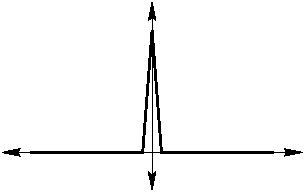
\includegraphics[width=0.3\textwidth]{ode/dirac/ddfunction}
  \end{center}
  \caption{The Dirac delta function.}
  \label{ddfunction}
\end{figure}






Let $f(x)$ be a continuous function that vanishes at infinity.
Consider the integral
\[ 
\int_{-\infty}^\infty f(x) \delta(x)\,\dd x. 
\]
We use integration by parts to evaluate the integral.
\begin{align*}
  \int_{-\infty}^\infty f(x) \delta(x)\,\dd x
  &= \big[ f(x) H(x) \big]_{-\infty}^\infty - \int_{-\infty}^\infty f'(x) H(x)\,\dd x 
  \\
  &= - \int_0^\infty f'(x)\,\dd x 
  \\
  &= [- f(x)]_0^\infty 
  \\
  &= f(0)
\end{align*}

We assumed that $f(x)$ vanishes at infinity in order to use integration
by parts to evaluate the integral.  However, since the delta function is zero
for $x \neq 0$, the integrand is nonzero only at $x = 0$.  Thus the behavior
of the function at infinity should not affect the value of the integral.  
Thus it is reasonable that $f(0) = \int_{-\infty}^\infty f(x)\delta(x)\,\dd x$ holds for
all continuous functions.
By changing variables and noting that $\delta(x)$ is symmetric we can derive 
a more general formula.
\begin{gather*}
  f(0) = \int_{-\infty}^\infty f(\xi) \delta(\xi)\,\dd \xi
  \\
  f(x) = \int_{-\infty}^\infty f(\xi + x) \delta(\xi)\,\dd \xi
  \\
  f(x) = \int_{-\infty}^\infty f(\xi) \delta(\xi - x)\,\dd \xi
  \\
  f(x) = \int_{-\infty}^\infty f(\xi) \delta(x - \xi)\,\dd \xi
\end{gather*}
This formula is very important in solving inhomogeneous differential equations.
%% CONTINUE cite green function



















%%===========================================================================
\section{The Delta Function as a Limit}


Consider a function $b(x,\epsilon)$ defined by
\[ 
b(x,\epsilon) = 
\begin{cases}
  0               &\mathrm{for}\ |x| > \epsilon/2 \\
  \frac{1}{\epsilon} \quad &\mathrm{for}\ |x| < \epsilon/2.
\end{cases}
\]
The graph of $b(x, 1/10)$ is shown in Figure~\ref{epsilon}.

\begin{figure}[h!]
  \begin{center}
    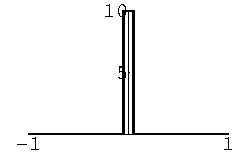
\includegraphics[width=0.3\textwidth]{ode/inhomogeneous/epsilon}
    \caption{Graph of the box function.}
    \label{epsilon}
  \end{center}
\end{figure}


The Dirac delta function $\delta(x)$ can be thought of as $b(x,\epsilon)$ in
the limit as $\epsilon \to 0$. 
Note that the delta function so defined satisfies the properties,
\[ 
\delta(x) = 
\begin{cases}
  0 & \mathrm{for}\ x \neq 0 \\
  \infty & \mathrm{for}\ x = 0
\end{cases}
\qquad \mathrm{and} \qquad
\int_{-\infty}^\infty \delta(x)\,\dd x = 1 
\]



\paragraph{Delayed Limiting Process.}
When the Dirac delta function appears inside an integral, we can think of the
delta function as a delayed limiting process. 
\[ 
\int_{-\infty}^\infty f(x) \delta(x)\,\dd x \equiv \lim_{\epsilon \to 0} \int_{-\infty}^\infty f(x) b(x, \epsilon)\,\dd x. 
\]
Let $f(x)$ be a continuous function and let $F'(x) = f(x)$.  
We compute the integral of $f(x) \delta(x)$.
\begin{align*}
  \int_{-\infty}^\infty f(x) \delta(x)\,\dd x
  &= \lim_{\epsilon \to 0} \frac{1}{\epsilon} \int_{-\epsilon/2}^{\epsilon/2} f(x)\,\dd x 
  \\
  &= \lim_{\epsilon \to 0} \frac{1}{\epsilon} [F(x)]_{-\epsilon/2}^{\epsilon/2} 
  \\
  &= \lim_{\epsilon \to 0} \frac{F(\epsilon/2) - F(-\epsilon/2)}{\epsilon} 
  \\
  &= F'(0) 
  \\
  &= f(0)
\end{align*}











%%===========================================================================
\section{Higher Dimensions}






We can define a Dirac delta function in $n$-dimensional Cartesian space, 
$\delta_n(\mathbf{x})$, $\mathbf{x} \in \mathbb{R}^n$.
It is defined by the following two properties.
\begin{gather*}
  \delta_n(\mathbf{x}) = 0 
  \quad \mathrm{for} \quad \mathbf{x} \neq \mathbf{0}
  \\
  \int_{\mathbb{R}^n} \delta_n(\mathbf{x}) \,\dd \mathbf{x} = 1
\end{gather*}
It is easy to verify, that the $n$-dimensional Dirac delta function can be 
written as a product of $1$-dimensional Dirac delta functions.
\[
\delta_n(\mathbf{x}) = \prod_{k=1}^n \delta(x_k)
\]





%%===========================================================================
\section{Non-Rectangular Coordinate Systems}




We can derive Dirac delta functions in non-rectangular coordinate systems
by making a change of variables in the relation,
\[
\int_{\mathbb{R}^n} \delta_n(\mathbf{x}) \,\dd \mathbf{x} = 1
\]
Where the transformation is non-singular, one merely divides the Dirac 
delta function by the Jacobian of the transformation to the coordinate system.




\begin{Example}
  Consider the Dirac delta function in cylindrical coordinates, $(r, \theta, z)$.
  The Jacobian is $J = r$.
  \[
  \int_{-\infty}^\infty \int_0^{2 \pi} \int_0^\infty \delta_3 \left( \mathbf{x} - \mathbf{x}_0 \right) 
  r \,\dd r \,\dd \theta \,\dd z = 1
  \]
  For $r_0 \neq 0$, the Dirac Delta function is
  \[
  \delta_3 \left( \mathbf{x} - \mathbf{x}_0 \right) 
  = \frac{1}{r} \delta \left( r - r_0 \right) \delta \left( \theta - \theta_0 \right)
  \delta \left( z - z_0 \right)
  \]
  since it satisfies the two defining properties.
  \[
  \frac{1}{r} \delta \left( r - r_0 \right) \delta \left( \theta - \theta_0 \right)
  \delta \left( z - z_0 \right) = 0 
  \quad \mathrm{for} \quad ( r, \theta, z ) \neq \left( r_0, \theta_0, z_0 \right)
  \]
  \begin{multline*}
    \int_{-\infty}^\infty \int_0^{2 \pi} \int_0^\infty \frac{1}{r} \delta \left( r - r_0 \right) \delta \left( \theta - \theta_0 \right)
    \delta \left( z - z_0 \right) r \,\dd r \,\dd \theta \,\dd z
    \\
    = \int_0^\infty \delta \left( r - r_0 \right) \,\dd r 
    \int_0^{2 \pi} \delta \left( \theta - \theta_0 \right) \,\dd \theta 
    \int_{-\infty}^\infty \delta \left( z - z_0 \right) \,\dd z = 1
  \end{multline*}
  For $r_0 = 0$, we have
  \[
  \delta_3 \left( \mathbf{x} - \mathbf{x}_0 \right) 
  = \frac{1}{2 \pi r} \delta \left( r \right) \delta \left( z - z_0 \right)
  \]
  since this again satisfies the two defining properties.
  \begin{gather*}
    \frac{1}{2 \pi r} \delta \left( r \right)
    \delta \left( z - z_0 \right) = 0 
    \quad \mathrm{for} \quad ( r, z ) \neq \left( 0, z_0 \right)
    \\
    \int_{-\infty}^\infty \int_0^{2 \pi} \int_0^\infty \frac{1}{2 \pi r} \delta \left( r \right) 
    \delta \left( z - z_0 \right) r \,\dd r \,\dd \theta \,\dd z
    = \frac{1}{2 \pi} \int_0^\infty \delta \left( r \right) \,\dd r 
    \int_0^{2 \pi} \,\dd \theta 
    \int_{-\infty}^\infty \delta \left( z - z_0 \right) \,\dd z = 1
  \end{gather*}
\end{Example}












\raggedbottom
%%===========================================================================
\exercises{
\pagebreak
\flushbottom
\section{Exercises}





\begin{Exercise}
  \label{exercise f0-f0+2=intfd}
  Let $f(x)$ be a function that is continuous except for a jump discontinuity
  at $x = 0$.  Using a delayed limiting process, show that
  \[ 
  \frac{f(0^-) + f(0^+)}{2} = \int_{-\infty}^\infty f(x)\delta(x)\,\dd x.
  \]

  \hintsolution{f0-f0+2=intfd}
\end{Exercise}



\begin{Exercise}
  \label{exercise ode dirac symmetric}
  Show that the Dirac delta function is symmetric.
  \[ 
  \delta(- x) = \delta(x)
  \]

  \hintsolution{ode dirac symmetric}
\end{Exercise}




\begin{Exercise}
  \label{exercise d(cx)=d(x)/c}
  Show that
  \[ 
  \delta(c x) = \frac{\delta(x)}{|c|}.
  \]

  \hintsolution{d(cx)=d(x)/c}
\end{Exercise}







\begin{Exercise}
  \label{exercise dcx=1cdx}
  We will consider the Dirac delta function with a function as on argument,
  $\delta(y(x))$.  Assume that $y(x)$ has simple zeros at the points $\{ x_n \}$.
  \[
  y(x_n) = 0, \quad y'(x_n) \neq 0
  \]
  Further assume that $y(x)$ has no multiple zeros.  (If $y(x)$ has multiple
  zeros $\delta(y(x))$ is not well-defined in the same sense that $1/0$ is not 
  well-defined.)
  Prove that 
  \[
  \delta(y(x)) = \sum_n \frac{\delta(x - x_n)}{|y'(x_n)|}.
  \]
  
  \hintsolution{dcx=1cdx}
\end{Exercise}







\begin{Exercise}
  \label{exercise ode dirac dnx}
  Justify the identity
  \[
  \int_{-\infty}^\infty f(x) \delta^{(n)}(x) \,\dd x = (-1)^n f^{(n)}(0)
  \]
  From this show that
  \[
  \delta^{(n)}(-x) = (-1)^n \delta^{(n)}(x)
  \quad \mathrm{and} \quad
  x \delta^{(n)}(x) = - n \delta^{(n-1)}(x).
  \]

  \hintsolution{ode dirac dnx}
\end{Exercise}









\begin{Exercise}
  \label{exercise ode dirac nd jacobian}
  Consider $\mathbf{x} = (x_1, \ldots, x_n) \in \mathbb{R}^n$ and the curvilinear
  coordinate system $\boldsymbol{\xi} = (\xi_1, \ldots, \xi_n)$.
  Show that
  \[
  \delta(\mathbf{x} - \mathbf{a}) = \frac{ \delta(\boldsymbol{\xi} - \boldsymbol{\alpha}) }{ |J| }
  \]
  where $\mathbf{a}$ and $\boldsymbol{\alpha}$ are corresponding points in the two 
  coordinate systems and $J$ is the Jacobian of the transformation
  from $\mathbf{x}$ to $\boldsymbol{\xi}$.
  \[
  J \equiv \frac{\partial \mathbf{x}}{\partial \boldsymbol{\xi}}
  \]

  \hintsolution{ode dirac nd jacobian}
\end{Exercise}






\begin{Exercise}
  \label{exercise dirac delta spherical}
  Determine the Dirac delta function in spherical coordinates, 
  $(r, \theta, \phi)$.
  \[
  x = r \cos \theta \sin \phi, \qquad
  y = r \sin \theta \sin \phi, \qquad
  z = r \cos \phi
  \]

  \hintsolution{dirac delta spherical}
\end{Exercise}














\raggedbottom
}
%%============================================================================
\hints{
\pagebreak
\flushbottom
\section{Hints}



\begin{Hint}
  \label{hint f0-f0+2=intfd}
  %% CONTINUE
\end{Hint}


\begin{Hint}
  \label{hint ode dirac symmetric}
  Verify that $\delta(-x)$ satisfies the two properties of the Dirac 
  delta function.
\end{Hint}



\begin{Hint}
  \label{hint d(cx)=d(x)/c}
  Evaluate the integral,
  \[
  \int_{-\infty}^\infty f(x) \delta(c x)\,\dd x,
  \]
  by noting that the Dirac delta function is symmetric
  and making a change of variables.
\end{Hint}



\begin{Hint}
  \label{hint dcx=1cdx}
  Let the points $\{ \xi_m \}$ partition the interval $(-\infty \ldots \infty)$ such that $y'(x)$
  is monotone on each interval $(\xi_m \ldots \xi_{m+1})$.  Consider some such interval,
  $(a \ldots b) \equiv (\xi_m \ldots \xi_{m+1})$.  Show that
  \[
  \int_a^b \delta(y(x))\,\dd x
  = \begin{cases}
    \int_\alpha^\beta \frac{\delta(y)}{|y'(x_n)|}\,\dd y &\mathrm{if}\ y(x_n) = 0\ 
    \mathrm{for}\ a < x_n < b \\
    0 &\mathrm{otherwise}
  \end{cases}
  \]
  for $\alpha = \min(y(a),y(b))$ and $\beta = \max(y(a),y(b))$.
  Now consider the integral on the interval $(-\infty \ldots \infty)$ as the sum of 
  integrals on the intervals $\{ (\xi_m \ldots \xi_{m+1}) \}$.
\end{Hint}




\begin{Hint}
  \label{hint ode dirac dnx}
  Justify the identity,
  \[
  \int_{-\infty}^\infty f(x) \delta^{(n)}(x) \,\dd x = (-1)^n f^{(n)}(0),
  \]
  with integration by parts.
  %% CONTINUE
\end{Hint}




\begin{Hint}
  \label{hint ode dirac nd jacobian}
  The Dirac delta function is defined by the following two properties.
  \begin{gather*}
    \delta(\mathbf{x} - \mathbf{a}) = 0 
    \quad \mathrm{for} \quad \mathbf{x} \neq \mathbf{a}
    \\
    \int_{\mathbb{R}^n} \delta(\mathbf{x} - \mathbf{a}) \,\dd \mathbf{x} = 1
  \end{gather*}
  Verify that $\delta(\boldsymbol{\xi} - \boldsymbol{\alpha}) / |J|$ satisfies these properties
  in the $\boldsymbol{\xi}$ coordinate system.
\end{Hint}





\begin{Hint}
  \label{hint dirac delta spherical}
  Consider the special cases $\phi_0 = 0,\pi$ and $r_0 = 0$.
\end{Hint}









\raggedbottom
}
%%============================================================================
\solutions{
\pagebreak
\flushbottom
\section{Solutions}








\begin{Solution}
  \label{solution f0-f0+2=intfd}
  Let $F'(x) = f(x)$.
  \begin{align*}
    \int_{-\infty}^\infty f(x)\delta(x)\,\dd x
    &= \lim_{\epsilon \to 0} \frac{1}{\epsilon} \int_{-\infty}^\infty f(x) b(x,\epsilon)\,\dd x 
    \\
    &= \lim_{\epsilon \to 0} \frac{1}{\epsilon} \left( \int_{-\epsilon/2}^0 f(x) b(x, \epsilon)\,\dd x 
      + \int_0^{\epsilon/2} f(x) b(x, \epsilon)\,\dd x \right) 
    \\
    &= \lim_{\epsilon \to 0} \frac{1}{\epsilon} \left( (F(0) - F(-\epsilon/2)) + (F(\epsilon/2) - F(0)) \right) 
    \\
    &= \lim_{\epsilon \to 0} \frac{1}{2} \left( \frac{F(0) - F(-\epsilon/2)}{\epsilon/2}
      + \frac{F(\epsilon/2) - F(0)}{\epsilon/2} \right) 
    \\
    &= \frac{F'(0^-) + F'(0^+)}{2} 
    \\
    &= \frac{f(0^-) + f(0^+)}{2}
  \end{align*}
\end{Solution}





\begin{Solution}
  \label{solution ode dirac symmetric}
  $\delta(-x)$ satisfies the two properties of the Dirac delta function.
  \begin{gather*}
    \delta(-x) = 0\ \mathrm{for}\ x \neq 0
    \\
    \int_{-\infty}^\infty \delta(-x)\,\dd x = \int_\infty^{-\infty} \delta(x) \,(-\dd x) = \int_{-\infty}^\infty \delta(-x)\,\dd x = 1
  \end{gather*}
  Therefore $\delta(-x) = \delta(x)$.
\end{Solution}






\begin{Solution}
  \label{solution d(cx)=d(x)/c}
  We note the the Dirac delta function is symmetric and we make a change of
  variables to derive the identity.
  \begin{align*}
    \int_{-\infty}^\infty \delta(c x)\,\dd x 
    &= \int_{-\infty}^\infty \delta(|c| x)\,\dd x 
    \\
    &= \int_{-\infty}^\infty \frac{\delta(x)}{|c|}\,\dd x 
  \end{align*}
  \[ 
  \boxed{
    \delta(c x) = \frac{\delta(x)}{|c|}
    }
  \]
\end{Solution}







\begin{Solution}
  \label{solution dcx=1cdx}
  Let the points $\{ \xi_m \}$ partition the interval $(-\infty \ldots \infty)$ such that $y'(x)$
  is monotone on each interval $(\xi_m \ldots \xi_{m+1})$.  Consider some such interval,
  $(a \ldots b) \equiv (\xi_m \ldots \xi_{m+1})$.  Note that $y'(x)$ is either 
  entirely positive or entirely negative in the interval.  First consider 
  the case when it is positive.  In this case $y(a) < y(b)$.
  \begin{align*}
    \int_a^b \delta(y(x))\,\dd x
    &= \int_{y(a)}^{y(b)} \delta(y) \left( \frac{\dd y}{\dd x} \right)^{-1} \,\dd y 
    \\
    &= \int_{y(a)}^{y(b)} \frac{\delta(y)}{y'(x)}\,\dd y 
    \\
    &= \begin{cases}
      \int_{y(a)}^{y(b)} \frac{\delta(y)}{y'(x_n)}\,\dd y &\mathrm{for}\ y(x_n) = 0\ 
      \mathrm{if}\ y(a) < 0 < y(b) \\
      0 &\mathrm{otherwise}
    \end{cases}
  \end{align*}
  Now consider the case that $y'(x)$ is negative on the interval so 
  $y(a) > y(b)$.
  \begin{align*}
    \int_a^b \delta(y(x))\,\dd x
    &= \int_{y(a)}^{y(b)} \delta(y) \left( \frac{\dd y}{\dd x} \right)^{-1} \,\dd y 
    \\
    &= \int_{y(a)}^{y(b)} \frac{\delta(y)}{y'(x)}\,\dd y 
    \\
    &= \int_{y(b)}^{y(a)} \frac{\delta(y)}{-y'(x)}\,\dd y 
    \\
    &= \begin{cases}
      \int_{y(b)}^{y(a)} \frac{\delta(y)}{-y'(x_n)}\,\dd y &\mathrm{for}\ y(x_n) = 0\ 
      \mathrm{if}\ y(b) < 0 < y(a) \\
      0 &\mathrm{otherwise}
    \end{cases}
  \end{align*}
  We conclude that
  \[
  \int_a^b \delta(y(x))\,\dd x
  = \begin{cases}
    \int_\alpha^\beta \frac{\delta(y)}{|y'(x_n)|}\,\dd y &\mathrm{if}\ y(x_n) = 0\ 
    \mathrm{for}\ a < x_n < b \\
    0 &\mathrm{otherwise}
  \end{cases}
  \]
  for $\alpha = \min(y(a),y(b))$ and $\beta = \max(y(a),y(b))$.

  Now we turn to the integral of $\delta(y(x))$ on $(-\infty \ldots \infty)$.
  Let $\alpha_m = \min(y(\xi_m),y(\xi_m))$ and $\beta_m = \max(y(\xi_m),y(\xi_m))$.
  \begin{align*}
    \int_{-\infty}^\infty \delta(y(x))\,\dd x
    &= \sum_m \int_{\xi_m}^{\xi_{m+1}} \delta(y(x))\,\dd x
    \\
    &= \sum_{\substack{m\\x_n \in (\xi_m \ldots \xi_{m+1})}} \int_{\xi_m}^{\xi_{m+1}} \delta(y(x))\,\dd x
    \\
    &= \sum_{\substack{m\\x_n \in (\xi_m \ldots \xi_{m+1})}} 
    \int_{\alpha_m}^{\beta_{m+1}} \frac{\delta(y)}{|y'(x_n)|}\,\dd y
    \\
    &= \sum_n \int_{-\infty}^\infty \frac{\delta(y)}{|y'(x_n)|}\,\dd y
    \\
    &= \int_{-\infty}^\infty \sum_n \frac{\delta(y)}{|y'(x_n)|}\,\dd y
  \end{align*}
  \[
  \boxed{
    \delta(y(x)) = \sum_n \frac{\delta(x - x_n)}{|y'(x_n)|}
    }
  \]
\end{Solution}






\begin{Solution}
  \label{solution ode dirac dnx}
  To justify the identity,
  \[
  \int_{-\infty}^\infty f(x) \delta^{(n)}(x) \,\dd x = (-1)^n f^{(n)}(0),
  \]
  we will use integration by parts.
  \begin{align*}
    \int_{-\infty}^\infty f(x) \delta^{(n)}(x) \,\dd x
    &= \left[ f(x) \delta^{(n-1)}(x) \right]_{-\infty}^\infty - \int_{-\infty}^\infty f'(x) \delta^{(n-1)}(x) \,\dd x
    \\
    &= - \int_{-\infty}^\infty f'(x) \delta^{(n-1)}(x) \,\dd x
    \\
    &= (-1)^n \int_{-\infty}^\infty f^{(n)}(x) \delta(x) \,\dd x
    \\
    &= (-1)^n f^{(n)}(0)
  \end{align*}

  CONTINUE HERE
  \[
  \delta^{(n)}(-x) = (-1)^n \delta^{(n)}(x)
  \quad \mathrm{and} \quad
  x \delta^{(n)}(x) = - n \delta^{(n-1)}(x).
  \]
\end{Solution}








\begin{Solution}
  \label{solution ode dirac nd jacobian}
  The Dirac delta function is defined by the following two properties.
  \begin{gather*}
    \delta(\mathbf{x} - \mathbf{a}) = 0 
    \quad \mathrm{for} \quad \mathbf{x} \neq \mathbf{a}
    \\
    \int_{\mathbb{R}^n} \delta(\mathbf{x} - \mathbf{a}) \,\dd \mathbf{x} = 1
  \end{gather*}
  We verify that $\delta(\boldsymbol{\xi} - \boldsymbol{\alpha}) / |J|$ satisfies these properties
  in the $\boldsymbol{\xi}$ coordinate system.
  \begin{align*}
    \frac{ \delta(\boldsymbol{\xi} - \boldsymbol{\alpha}) }{ |J| }
    &= \frac{ \delta(\xi_1 - \alpha_1) \cdots \delta(\xi_n - \alpha_n) }{ |J| }
    \\
    &= 0 \quad \mathrm{for} \quad \boldsymbol{\xi} \neq \boldsymbol{\alpha}
  \end{align*}
  \begin{align*}
    \int \frac{ \delta(\boldsymbol{\xi} - \boldsymbol{\alpha}) }{ |J| }|J|\,\dd \boldsymbol{\xi}
    &= \int \delta(\boldsymbol{\xi} - \boldsymbol{\alpha}) \,\dd \boldsymbol{\xi}
    \\
    &= \int \delta(\xi_1 - \alpha_1) \cdots \delta(\xi_n - \alpha_n) \,\dd \boldsymbol{\xi}
    \\
    &= \int \delta(\xi_1 - \alpha_1)\,\dd \xi_1 \cdots \int \delta(\xi_n - \alpha_n)\,\dd \xi_n
    \\
    &= 1
  \end{align*}
  We conclude that $\delta(\boldsymbol{\xi} - \boldsymbol{\alpha}) / |J|$ is the Dirac delta function
  in the $\boldsymbol{\xi}$ coordinate system.
  \[
  \delta(\mathbf{x} - \mathbf{a}) = \frac{ \delta(\boldsymbol{\xi} - \boldsymbol{\alpha}) }{ |J| }
  \]
\end{Solution}






\begin{Solution}
  \label{solution dirac delta spherical}
  We consider the Dirac delta function in spherical coordinates, $(r, \theta, \phi)$.
  The Jacobian is $J = r^2 \sin(\phi)$.
  \[
  \int_0^\pi \int_0^{2 \pi} \int_0^\infty \delta_3 \left( \mathbf{x} - \mathbf{x}_0 \right) 
  r^2 \sin(\phi) \,\dd r \,\dd \theta \,\dd \phi = 1
  \]
  For $r_0 \neq 0$, and $\phi_0 \neq 0,\pi$, the Dirac Delta function is
  \[
  \delta_3 \left( \mathbf{x} - \mathbf{x}_0 \right) 
  = \frac{1}{r^2 \sin(\phi)} \delta \left( r - r_0 \right) \delta \left( \theta - \theta_0 \right)
  \delta \left( \phi - \phi_0 \right)
  \]
  since it satisfies the two defining properties.
  \[
  \frac{1}{r^2 \sin(\phi)} \delta \left( r - r_0 \right) \delta \left( \theta - \theta_0 \right)
  \delta \left( \phi - \phi_0 \right) = 0 
  \quad \mathrm{for} \quad ( r, \theta, \phi ) \neq \left( r_0, \theta_0, \phi_0 \right)
  \]
  \begin{multline*}
    \int_0^\pi \int_0^{2 \pi} \int_0^\infty \frac{1}{r^2 \sin(\phi)} 
    \delta \left( r - r_0 \right) \delta \left( \theta - \theta_0 \right) \delta \left( \phi - \phi_0 \right)
    r^2 \sin(\phi) \,\dd r \,\dd \theta \,\dd \phi
    \\
    = \int_0^\infty \delta \left( r - r_0 \right) \,\dd r 
    \int_0^{2 \pi} \delta \left( \theta - \theta_0 \right) \,\dd \theta 
    \int_0^\pi \delta \left( \phi - \phi_0 \right) \,\dd \phi = 1
  \end{multline*}
  For $\phi_0 = 0$ or $\phi_0 = \pi$, the Dirac delta function is
  \[
  \delta_3 \left( \mathbf{x} - \mathbf{x}_0 \right) 
  = \frac{1}{2 \pi r^2 \sin(\phi)} \delta \left( r - r_0 \right) \delta \left( \phi - \phi_0 \right).
  \]
  We check that the value of the integral is unity.
  \begin{multline*}
    \int_0^\pi \int_0^{2 \pi} \int_0^\infty \frac{1}{2 \pi r^2 \sin(\phi)} 
    \delta \left( r - r_0 \right) \delta \left( \phi - \phi_0 \right)
    r^2 \sin(\phi) \,\dd r \,\dd \theta \,\dd \phi
    \\
    = \frac{1}{2 \pi} \int_0^\infty \delta \left( r - r_0 \right) \,\dd r 
    \int_0^{2 \pi} \,\dd \theta 
    \int_0^\pi \delta \left( \phi - \phi_0 \right) \,\dd \phi = 1
  \end{multline*}
  For $r_0 = 0$ the Dirac delta function is
  \[
  \delta_3 \left( \mathbf{x} \right) 
  = \frac{1}{4 \pi r^2} \delta \left( r \right)
  \]
  We verify that the value of the integral is unity.
  \[
  \int_0^\pi \int_0^{2 \pi} \int_0^\infty \frac{1}{4 \pi r^2} 
  \delta \left( r - r_0 \right) r^2 \sin(\phi) \,\dd r \,\dd \theta \,\dd \phi
  = \frac{1}{4 \pi} \int_0^\infty \delta \left( r \right) \,\dd r 
  \int_0^{2 \pi} \,\dd \theta 
  \int_0^\pi \sin(\phi) \,\dd \phi = 1
  \]
\end{Solution}












\raggedbottom
}


\flushbottom

%%
%% Prove the assertion in the paragraph before the result on Fredholm Alt. Thrm.
%%
%% Consider adding  a section on Modified Green Functions.
%%
%% Before presenting the Fredholm alternative theorem.  Do the analogous 
%% work for the inhomogeneous matrix equation.  State the existence, 
%% uniqueness results for Ax=b in terms of the eigenvectors of A.
%%




%%============================================================================
%%============================================================================
\chapter{Inhomogeneous Differential Equations}
\label{chapter_io}

Feelin' stupid?  I know I am!

\begin{flushright}
  -Homer Simpson
\end{flushright}








%%============================================================================
\section{Particular Solutions}
\index{particular solution!of an ODE}



Consider the $n^{\mathrm{th}}$ order linear homogeneous equation
\[
L[y] \equiv y^{(n)} + p_{n-1}(x) y^{(n-1)} + \cdots + p_1(x) y' + p_0(x) y = 0.
\]
Let $\{y_1, y_2, \ldots, y_n\}$ be a set of linearly independent 
homogeneous solutions, $L[y_k]=0$.  We know that the general solution of 
the homogeneous equation is a linear combination of the homogeneous solutions.
\[
y_h = \sum_{k=1}^n c_k y_k(x)
\]


Now consider the $n^{t h}$ order linear \textit{inhomogeneous} equation
\[
L[y] \equiv y^{(n)} + p_{n-1}(x) y^{(n-1)} + \cdots + p_1(x) y' + p_0(x) y = f(x).
\]
Any function $y_p$ which satisfies this equation is called a 
\textit{particular solution} of the differential equation.
We want to know the general solution of the inhomogeneous equation.
Later in this chapter we will cover methods of constructing this solution;
now we consider the form of the solution.  


Let $y_p$ be a particular solution.  Note that $y_p + h$ is a particular 
solution if $h$ satisfies the homogeneous equation.
\[
L[y_p + h] = L[y_p] + L[h] = f + 0 = f
\]
Therefore $y_p + y_h$ satisfies the homogeneous equation.  We show that this is
the general solution of the inhomogeneous equation.
Let $y_p$ and $\eta_p$ both be solutions
of the inhomogeneous equation $L[y] = f$.  The difference of $y_p$ and
$\eta_p$ is a homogeneous solution.
\[
L[y_p - \eta_p] = L[y_p] - L[\eta_p] = f - f = 0
\]
$y_p$ and $\eta_p$ differ by a linear combination of the homogeneous solutions
$\{ y_k \}$.  Therefore the general solution of $L[y] = f$ is the sum of any 
particular solution $y_p$ and the general homogeneous solution $y_h$.
\[
y_p + y_h = y_p(x) + \sum_{k=1}^n c_k y_k(x)
\]




\begin{Result}
  The general solution of the $n^{t h}$ order linear inhomogeneous equation
  $L[y] = f(x)$ is
  \[ 
  y = y_p + c_1 y_1 + c_2 y_2 + \cdots + c_n y_n,
  \]
  where $y_p$ is a particular solution, $\{y_1, \ldots,y_n\}$ is a set of
  linearly independent homogeneous solutions, and the $c_k$'s 
  are arbitrary constants.
\end{Result}






\begin{Example}
  The differential equation 
  \[ 
  y'' + y = \sin(2 x)
  \]
  has the two homogeneous solutions
  \[ 
  y_1 = \cos x, \qquad y_2 = \sin x,
  \]
  and a particular solution
  \[ 
  y_p = -\frac{1}{3} \sin(2 x).
  \]
  We can add any combination of the homogeneous solutions to $y_p$ and it will
  still be a particular solution.  For example,
  \begin{align*}
    \eta_p &= -\frac{1}{3} \sin(2 x) - \frac{1}{3} \sin x \\
    &= -\frac{2}{3} \sin\left(\frac{3x}{2}\right)
    \cos\left(\frac{x}{2}\right)
  \end{align*}
  is a particular solution.
\end{Example}























%%============================================================================
\section{Method of Undetermined Coefficients}



The first method we present for computing particular solutions is the
\textit{method of undetermined coefficients}.
For some simple differential equations, (primarily constant coefficient 
equations), and some simple inhomogeneities we are able to guess the form
of a particular solution.  This form will contain some unknown parameters.
We substitute this form into the differential equation to determine 
the parameters and thus determine a particular solution.

Later in this chapter we will present general methods which work for any 
linear differential equation and any inhogeneity.  Thus one might wonder why
I would present a method that works only for some simple problems. (And
why it is called a ``method'' if it amounts to no more than guessing.)
The answer is that guessing an answer is less grungy than computing it
with the formulas we will develop later.  Also, the process of this guessing
is not random, there is rhyme and reason to it.


Consider an $n^{\mathrm{th}}$ order constant coefficient, inhomogeneous equation.
\[
L[y] \equiv y^{(n)} + a_{n-1} y^{(n-1)} + \cdots + a_1 y' + a_0 y = f(x)
\]
If $f(x)$ is one of a few simple forms, then we can guess the form of a 
particular solution.  Below we enumerate some cases.

\begin{description}
\item[$\mathbf{ f = p(x) }$.]
  If $f$ is an $m^{\mathrm{th}}$ order polynomial, $f(x) = p_m x^m + \cdots + p_1 x + p_0$,
  then guess
  \[
  y_p = c_m x^m + \cdots c_1 x + c_0.
  \]
\item[$\mathbf{ f = p(x) \,\mathbf{e}^{a x} }$.]
  If $f$ is a polynomial times an exponential then guess
  \[
  y_p = ( c_m x^m + \cdots c_1 x + c_0 ) \e^{a x}.
  \]
\item[$\mathbf{ f = p(x) \,\mathbf{e}^{a x} \,\mathbf{cos}\,(b x) }$.]
  If $f$ is a cosine or sine times a polynomial and perhaps an exponential, 
  $f(x) = p(x) \e^{a x} \cos(b x)$ or $f(x) = p(x) \e^{a x} \sin(b x)$
  then guess
  \[
  y_p = ( c_m x^m + \cdots c_1 x + c_0 ) \e^{a x} \cos(b x) 
  + ( d_m x^m + \cdots d_1 x + d_0 ) \e^{a x} \sin(b x).
  \]
  Likewise for hyperbolic sines and hyperbolic cosines.
\end{description}




\begin{Example}
  Consider
  \[
  y'' - 2 y' + y = t^2.
  \]
  The homogeneous solutions are $y_1 = \e^t$ and $y_2 = t \e^t$.
  We guess a particular solution of the form
  \[
  y_p = a t^2 + b t + c.
  \]
  We substitute the expression into the differential equation 
  and equate coefficients of powers of $t$ to determine the parameters.
  \begin{gather*}
    y_p'' - 2 y_p' + y_p = t^2 \\
    (2 a) - 2 (2 a t + b) + (a t^2 + b t + c) = t^2 \\
    (a - 1) t^2 + (b - 4 a) t + (2 a - 2 b + c) = 0 \\
    a - 1 = 0, \quad b - 4 a = 0, \quad 2 a - 2 b + c = 0 \\
    a = 1, \quad b = 4, \quad c = 6
  \end{gather*}
  A particular solution is
  \[
  y_p = t^2 + 4 t + 6.
  \]
\end{Example}




If the inhomogeneity is a sum of terms, $L[y] = f \equiv f_1 + \cdots + f_k$,
you can solve the problems $L[y] = f_1,\ \ldots \ ,L[y] = f_k$ independently 
and then take the sum of the solutions as a particular solution of
$L[y] = f$.



\begin{Example}
  Consider
  \begin{equation}
    \label{y2yyt2e2t}
    L[y] \equiv y'' - 2 y' + y = t^2 + \e^{2 t}.
  \end{equation}
  The homogeneous solutions are $y_1 = \e^t$ and $y_2 = t \e^t$.
  We already know a particular solution to $L[y] = t^2$.  
  We seek a particular solution to $L[y] = \e^{2 t}$.
  We guess a particular solution of the form
  \[
  y_p = a \e^{2 t}.
  \]
  We substitute the expression into the differential equation 
  to determine the parameter.
  \begin{gather*}
    y_p'' - 2 y_p' + y_p = \e^{2 t} \\
    4 a e^{2 t} - 4 a \e^{2 t} + a \e^{2 t} = \e^{2 t} \\
    a = 1
  \end{gather*}
  A particular solution of $L[y] = \e^{2 t}$ is $y_p = \e^{2 t}$.
  Thus a particular solution of Equation~\ref{y2yyt2e2t} is
  \[
  y_p = t^2 + 4 t + 6 + \e^{2 t}.
  \]
\end{Example}




The above guesses will not work if the inhomogeneity is a homogeneous 
solution.  In this case, multiply the guess by the lowest power of $x$ such
that the guess does not contain homogeneous solutions.





\begin{Example}
  Consider
  \[
  L[y] \equiv y'' - 2 y' + y = \e^t.
  \]
  The homogeneous solutions are $y_1 = \e^t$ and $y_2 = t \e^t$.
  Guessing a particular solution of the form $y_p = a \e^t$ would not
  work because $L[\e^t] = 0$.
  We guess a particular solution of the form
  \[
  y_p = a t^2 \e^t
  \]
  We substitute the expression into the differential equation 
  and equate coefficients of like terms to determine the parameters.
  \begin{gather*}
    y_p'' - 2 y_p' + y_p = \e^t \\
    (a t^2 + 4 a t + 2 a) \e^t - 2 (a t^2 + 2 a t) \e^t + a t^2 \e^t = \e^t \\
    2 a \e^t = \e^t \\
    a = \frac{1}{2}
  \end{gather*}
  A particular solution is
  \[
  y_p = \frac{t^2}{2} \e^t.
  \]
\end{Example}





\begin{Example}
  Consider
  \[
  y'' + \frac{1}{x} y' + \frac{1}{x^2} y = x, \quad x > 0.
  \]
  The homogeneous solutions are $y_1 = \cos(\ln x)$ and $y_2 = \sin(\ln x)$.
  We guess a particular solution of the form
  \[
  y_p = a x^3
  \]
  We substitute the expression into the differential equation 
  and equate coefficients of like terms to determine the parameter.
  \begin{gather*}
    y_p'' + \frac{1}{x} y_p' + \frac{1}{x^2} y_p = x
    \\
    6 a x + 3 a x + a x = x
    \\
    a = \frac{1}{10}
  \end{gather*}
  A particular solution is
  \[
  y_p = \frac{x^3}{10}.
  \]
\end{Example}









%%============================================================================
\section{Variation of Parameters}



In this section we present a method for computing a particular solution of
an inhomogeneous equation given that we know the homogeneous solutions.
We will first consider second order equations and then generalize the result
for $n^{\mathrm{th}}$ order equations.




%%-----------------------------------------------------------------------------
\subsection{Second Order Differential Equations}




Consider the second order inhomogeneous equation,
\[
L[y] \equiv y'' + p(x)y' + q(x)y = f(x), \quad \mathrm{on}\ a < x < b.
\]
We assume that the coefficient functions in the differential equation are
continuous on $[a \ldots b]$.
Let $y_1(x)$ and $y_2(x)$ be two linearly independent solutions to the
homogeneous equation.  Since the Wronskian,
\[
W(x) = \exp \left( - \int p(x) \,\dd x \right),
\]
is non-vanishing, we know that these solutions exist.
We seek a particular solution of the form,
\[
y_p = u_1(x) y_1 + u_2(x) y_2.
\]
We compute the derivatives of $y_p$.
\begin{gather*}
  y_p' = u_1' y_1 + u_1 y_1' + u_2' y_2 + u_2 y_2' \\
  y_p'' = u_1'' y_1 + 2 u_1' y_1' + u_1 y_1'' + u_2'' y_2 + 2 u_2'y_2' + u_2 y_2''
\end{gather*}
We substitute the expression for $y_p$ and its derivatives into the 
inhomogeneous equation and use the fact that $y_1$ and $y_2$ are homogeneous
solutions to simplify the equation.
\begin{gather*}
  u_1'' y_1 + 2 u_1' y_1' + u_1 y_1'' + u_2'' y_2 + 2 u_2'y_2' + u_2 y_2''
  + p ( u_1' y_1 + u_1 y_1' + u_2' y_2 + u_2 y_2' )
  + q ( u_1 y_1 + u_2 y_2 ) = f \\
  u_1'' y_1 + 2 u_1' y_1' + u_2'' y_2 + 2 u_2'y_2'
  + p ( u_1' y_1 + u_2' y_2 ) = f
\end{gather*}
This is an ugly equation for $u_1$ and $u_2$, however, we have an ace up our 
sleeve.
Since $u_1$ and $u_2$ are undetermined functions of $x$, we are free to impose
a constraint.  We choose this constraint to simplify the algebra.
\[
u_1' y_1 + u_2' y_2 = 0
\]
This constraint simplifies the derivatives of $y_p$,
\begin{align*}
  y_p'    &= u_1' y_1 + u_1 y_1' + u_2' y_2 + u_2 y_2' \\
  &= u_1 y_1' + u_2 y_2' \\
  y_p''   &= u_1' y_1' + u_1 y_1'' + u_2'y_2' + u_2 y_2''.
\end{align*}
We substitute the new expressions for $y_p$ and its derivatives into the 
inhomogeneous differential equation to obtain a much simpler equation than 
before.
\begin{gather*}
  u_1' y_1' + u_1 y_1'' + u_2' y_2' + u_2 y_2'' + p (u_1 y_1' + u_2 y_2')
  + q (u_1 y_1 + u_2 y_2) = f(x) \\
  u_1' y_1' + u_2' y_2' + u_1 L[y_1] + u_2 L[y_2] = f(x) \\
  u_1' y_1' + u_2' y_2' = f(x).
\end{gather*}

With the constraint, we have a system of linear equations for $u_1'$ and $u_2'$.
\begin{align*}
  u_1'y_1  + u_2'y_2  &= 0 \\
  u_1'y_1' + u_2'y_2' &= f(x).  
\end{align*}
\[
\begin{pmatrix}
  y_1 & y_2 \\
  y_1' & y_2'
\end{pmatrix}
\begin{pmatrix}
  u_1' \\
  u_2'
\end{pmatrix}
=
\begin{pmatrix}
  0 \\
  f
\end{pmatrix}
\]
We solve this system using Kramer's rule.
(See Appendix~\ref{appendix formulas from linear algebra}.)
\[
u_1' = -\frac{f(x)y_2}{W(x)} \qquad  u_2' = \frac{f(x)y_1}{W(x)}
\]
Here $W(x)$ is the Wronskian.
\[
W(x) =
\begin{vmatrix}
  y_1 & y_2 \\
  y_1' & y_2'
\end{vmatrix}
\]
We integrate to get $u_1$ and $u_2$.  This gives us a particular solution.
\[ 
y_p = -y_1 \int \frac{f(x) y_2(x)}{W(x)}\,\dd x +
y_2 \int \frac{f(x) y_1(x)}{W(x)}\,\dd x. 
\]






\begin{Result}
  Let $y_1$ and $y_2$ be linearly independent homogeneous solutions of
  \[
  L[y] = y'' + p(x)y' + q(x)y = f(x).
  \]
  A particular solution is
  \[ 
  y_p = -y_1(x) \int \frac{f(x) y_2(x)}{W(x)}\,\dd x +
  y_2(x) \int \frac{f(x) y_1(x)}{W(x)}\,\dd x, 
  \]
  where $W(x)$ is the Wronskian of $y_1$ and $y_2$.
\end{Result}








\begin{Example}
  Consider the equation,
  \[ 
  y'' + y = \cos(2x).
  \]
  The homogeneous solutions are $y_1 = \cos x$ and $y_2 = \sin x$.
  We compute the Wronskian.
  \[ 
  W(x) 
  = \begin{vmatrix}
    \cos x & \sin x \\
    -\sin x & \cos x
  \end{vmatrix}
  = \cos^2 x + \sin^2 x 
  = 1
  \]
  We use variation of parameters to find a particular solution.
  \begin{align*}
    y_p     &= - \cos(x) \int \cos(2 x)\sin(x)\,\dd x
    + \sin(x) \int \cos(2 x)\cos(x)\,\dd x \\
    &= -\frac{1}{2} \cos(x) \int \big( \sin(3 x) - \sin(x) \big) \,\dd x
    + \frac{1}{2} \sin(x) \int \big( \cos(3 x)+ \cos(x) \big) \,\dd x \\
    &= -\frac{1}{2} \cos(x) \left(-\frac{1}{3}\cos(3x) + \cos(x) \right)
    + \frac{1}{2} \sin(x) \left(\frac{1}{3} \sin(3x)
      + \sin(x) \right) \\
    &= \frac{1}{2} \big(\sin^2(x) - \cos^2(x) \big)
    + \frac{1}{6} \big(\cos(3x)\cos(x) + \sin(3x)\sin(x) \big) \\
    &= -\frac{1}{2} \cos(2x)
    + \frac{1}{6} \cos(2x) \\
    &= -\frac{1}{3} \cos(2x)
  \end{align*}
  The general solution of the inhomogeneous equation is
  \[ 
  \boxed{
    y = -\frac{1}{3} \cos(2x) + c_1 \cos(x) + c_2 \sin(x).
    } 
  \]
\end{Example}











%%-----------------------------------------------------------------------------
\subsection{Higher Order Differential Equations}





Consider the $n^{th}$ order inhomogeneous equation,
\[
L[y] = y{(n)} + p_{n-1}(x) y^{(n-1)} + \cdots + p_1(x) y' + p_0(x) y = f(x), 
\quad \mathrm{on}\ a < x < b.
\]
We assume that the coefficient functions in the differential equation are
continuous on $[a \ldots b]$.
Let $\{y_1, \ldots, y_n\}$ be a set of linearly independent solutions to the
homogeneous equation.  Since the Wronskian,
\[
W(x) = \exp \left( - \int p_{n-1}(x) \,\dd x \right),
\]
is non-vanishing, we know that these solutions exist.
We seek a particular solution of the form
\[
y_p = u_1 y_1 + u_2 y_2 + \cdots + u_n y_n.
\]
Since $\{u_1,\ldots,u_n\}$ are undetermined functions of $x$, 
we are free to impose $n-1$ constraints.
We choose these constraints to simplify the algebra.
\begin{alignat*}{5}
  &u_1' y_1 &+ &u_2' y_2  &+ &\cdots &+ &u_n' y_n &= &0 \\
  &u_1' y_1' &+ &u_2' y_2'  &+ &\cdots &+ &u_n' y_n' &= &0 \\
  &\ \ \vdots &+ &\ \ \vdots &+ &\ \ \vdots &+ &\ \ \vdots    &= &0 \\
  &u_1' y_1^{(n-2)} &+ &u_2' y_2^{(n-2)}  &+ &\cdots &+ &u_n' y_n^{(n-2)} &= &0 
\end{alignat*}
We differentiate the expression for $y_p$, utilizing our constraints.
\begin{alignat*}{5}
  &y_p &= &u_1 y_1 &+ &u_2 y_2 &+ &\cdots &+ &u_n y_n \\
  &y_p' &= &u_1 y_1' &+ &u_2 y_2' &+ &\cdots &+ &u_n y_n' \\
  &y_p'' &= &u_1 y_1'' &+ &u_2 y_2'' &+ &\cdots &+ &u_n y_n'' \\
  &\ \ \vdots &= &\ \ \vdots   &+ &\ \ \vdots    &+ &\ \ \vdots &+ &\ \ \vdots \\
  &y_p^{(n)} &= &u_1 y_1^{(n)} &+ &u_2 y_2^{(n)} &+ &\cdots &+ &u_n y_n^{(n)} 
  +u_1' y_1^{(n-1)} + u_2' y_2^{(n-1)} + \cdots + u_n' y_n^{(n-1)} 
\end{alignat*}
We substitute $y_p$ and its derivatives into the inhomogeneous differential 
equation and use the fact that the $y_k$ are homogeneous solutions.
\begin{gather*}
  u_1 y_1^{(n)} + \cdots + u_n y_n^{(n)} + u_1' y_1^{(n-1)} + \cdots + u_n' y_n^{(n-1)} 
  + p_{n-1} ( u_1 y_1^{(n-1)} + \cdots + u_n y_n^{(n-1)} )
  + \cdots
  + p_0 ( u_1 y_1 + \cdots u_n y_n ) = f \\
  u_1 L[y_1] + u_2 L[y_2] + \cdots + u_n L[y_n] 
  + u_1' y_1^{(n-1)} + u_2' y_2^{(n-1)} + \cdots + u_n' y_n^{(n-1)} 
  = f \\
  u_1' y_1^{(n-1)} + u_2' y_2^{(n-1)} + \cdots + u_n' y_n^{(n-1)} = f. 
\end{gather*}

With the constraints, we have a system of linear equations for
$\{ u_1, \ldots, u_n \}$.
\[
\begin{pmatrix}
  y_1 & y_2 & \cdots & y_n \\
  y_1' & y_2' & \cdots & y_n' \\
  \vdots & \vdots & \ddots & \vdots \\
  y_1^{(n-1)} & y_2^{(n-1)} & \cdots & y_n^{(n-1)} 
\end{pmatrix}
\begin{pmatrix}
  u_1' \\
  u_2' \\
  \vdots \\
  u_n'
\end{pmatrix}
=
\begin{pmatrix}
  0 \\
  \vdots \\
  0 \\
  f
\end{pmatrix}.
\]
We solve this system using Kramer's rule.
(See Appendix~\ref{appendix formulas from linear algebra}.)
\[
u_k' = (-1)^{n+k+1} \frac{W[y_1,\ldots,y_{k-1},y_{k+1},\ldots,y_n]}
{W[y_1,y_2,\ldots,y_n]} f, \quad \mathrm{for}\ k=1,\ldots,n,
\]
Here $W$ is the Wronskian.

We integrating to obtain the $u_k$'s.
\[ 
u_k = (-1)^{n+k+1} \int \frac{W[y_1,\ldots,y_{k-1},y_{k+1},\ldots,y_n](x)}
{W[y_1,y_2,\ldots,y_n](x)} f(x) \,\dd x, 
\quad \mathrm{for}\ k = 1,\ldots,n
\]



\begin{Result}
  \label{ionvop}
  Let $\{y_1,\ldots,y_n\}$ be linearly independent homogeneous solutions of
  \[
  L[y] = y{(n)} + p_{n-1}(x) y^{(n-1)} + \cdots + p_1(x) y' + p_0(x) y = f(x), 
  \quad \mathrm{on}\ a < x < b.
  \]
  A particular solution is
  \[
  y_p = u_1 y_1 + u_2 y_2 + \cdots + u_n y_n.
  \]
  where
  \[ 
  u_k = (-1)^{n+k+1} \int \frac{W[y_1,\ldots,y_{k-1},y_{k+1},\ldots,y_n](x)}
  {W[y_1,y_2,\ldots,y_n](x)} f(x) \,\dd x,\ 
  \mathrm{for}\ k = 1,\ldots,n,
  \]
  and $W[y_1,y_2,\ldots,y_n](x)$ is the Wronskian of $\{y_1(x),\ldots, y_n(x)\}$.
\end{Result}








%%=============================================================================
\section{Piecewise Continuous Coefficients and Inhomogeneities}



\begin{Example}
  Consider the problem
  \[ 
  y'' - y = \e^{-\alpha |x| }, \qquad y(\pm \infty) = 0, \qquad \alpha > 0, \alpha \neq 1.
  \]
  The homogeneous solutions of the differential equation are $\e^x$ and $\e^{-x}$.
  We use variation of parameters to find a particular solution for $x > 0$.
  \begin{align*}
    y_p &= - \e^x \int^x \frac{\e^{-\xi} \e^{-\alpha \xi}}{-2} \,\dd \xi
    + \e^{-x} \int^x \frac{\e^\xi \e^{-\alpha \xi}}{-2}\,\dd \xi 
    \\
    &= \frac{1}{2} \e^x \int^x \e^{-(\alpha+1)\xi}\,\dd \xi
    - \frac{1}{2} \e^{-x} \int^x \e^{(1-\alpha)\xi} \,\dd \xi 
    \\
    &= - \frac{1}{2(\alpha+1)} \e^{-\alpha x}
    + \frac{1}{2(\alpha-1)} \e^{-\alpha x} 
    \\
    &= \frac{\e^{-\alpha x}}{\alpha^2 - 1}, \quad \mathrm{for}\ x > 0
  \end{align*}
  A particular solution for $x < 0$ is
  \[
  y_p = \frac{\e^{\alpha x}}{\alpha^2 - 1}, \quad \mathrm{for}\ x < 0.
  \]
  Thus a particular solution is
  \[
  y_p = \frac{\e^{-\alpha |x|}}{\alpha^2 - 1}.
  \]

  The general solution is
  \[ 
  y = \frac{1}{\alpha^2-1} \e^{-\alpha |x|} + c_1 \e^x + c_2 \e^{-x}. 
  \]
  Applying the boundary conditions, we see that $c_1 = c_2 = 0$.  
  Apparently the solution is
  \[ 
  y = \frac{\e^{-\alpha |x|}}{\alpha^2-1}.
  \]
  This function is plotted in Figure~\ref{wrong_right_sol}.  This
  function satisfies the differential equation for positive and negative
  $x$.  It also satisfies the boundary conditions.  However, this is NOT
  a solution to the differential equation.  Since the differential
  equation has no singular points and the inhomogeneous term is
  continuous, the solution must be twice continuously differentiable.
  Since the derivative of $\e^{-\alpha |x|} / (\alpha^2-1)$ has a jump
  discontinuity at $x = 0$, the second derivative does not exist.  Thus
  this function could not possibly be a solution to the differential
  equation.  In the next example we examine the right way to solve this
  problem.
\end{Example}





\begin{figure}[tb!]
  \begin{center}
    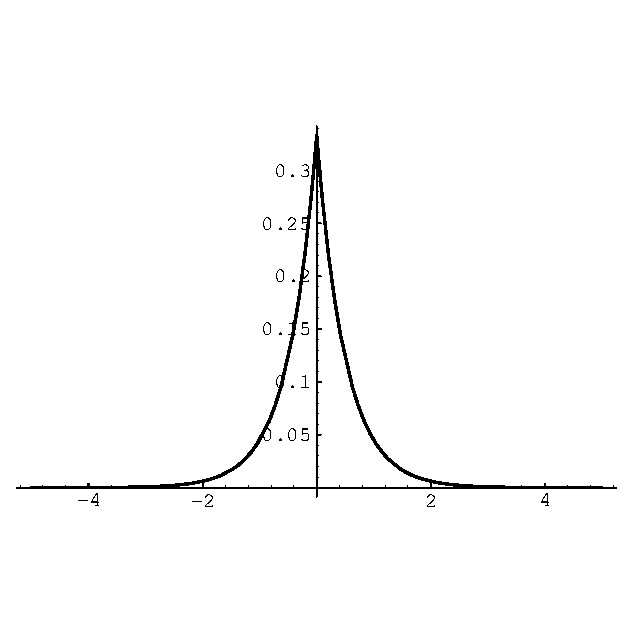
\includegraphics[width=0.4\textwidth]{ode/inhomogeneous/wrongsol}
    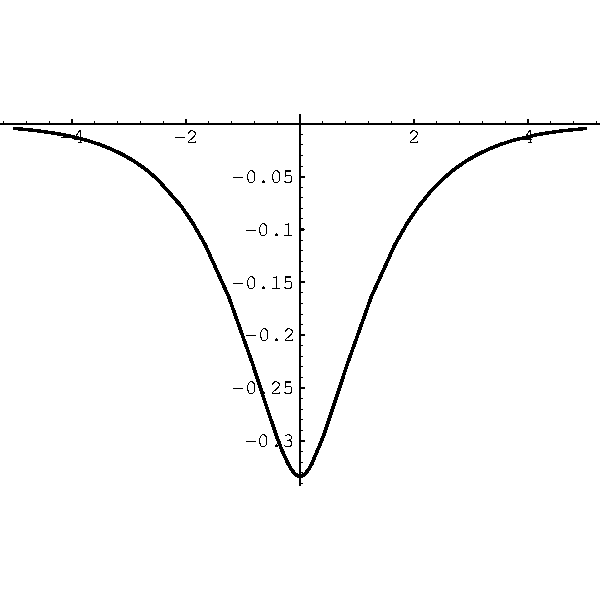
\includegraphics[width=0.4\textwidth]{ode/inhomogeneous/rightsol}
  \end{center}
  \caption{The incorrect and correct solution to the differential equation.}
  \label{wrong_right_sol}
\end{figure}







\begin{Example}
  Again consider
  \[ 
  y'' - y = \e^{-\alpha |x|}, \qquad y(\pm \infty) = 0, \qquad \alpha > 0, \alpha \neq 1. 
  \]
  Separating this into two problems for positive and negative $x$,
  \begin{alignat*}{3}
    y_-'' - y_- &= \e^{\alpha x}, &\quad &y_-(-\infty) = 0, &\quad &\mathrm{on}\ -\infty < x \leq 0, \\
    y_+'' - y_+ &= \e^{-\alpha x}, &\quad &y_+(\infty)=0, &\quad &\mathrm{on}\ 0\leq x < \infty.
  \end{alignat*}
  In order for the solution over the whole domain to be twice
  differentiable, the solution and its first derivative must be
  continuous.  Thus we impose the additional boundary conditions
  \[ 
  y_-(0) = y_+(0), \qquad y_-'(0) = y_+'(0). 
  \]
  The solutions that satisfy the two differential equations and the 
  boundary conditions at infinity are
  \[ 
  y_- = \frac{\e^{\alpha x}}{\alpha^2-1} + c_- \e^x, \qquad
  y_+ = \frac{\e^{-\alpha x}}{\alpha^2-1} + c_+ \e^{-x}. 
  \]
  The two additional boundary conditions give us the equations
  \begin{alignat*}{3}
    y_-(0) &= y_+(0) &\quad &\to &\quad &c_- = c_+ \\
    y_-'(0) &= y_+'(0) &\quad &\to &\quad &\frac{\alpha}{\alpha^2-1} + c_- = 
    -\frac{\alpha}{\alpha^2-1} - c_+.
  \end{alignat*}
  We solve these two equations to determine $c_-$ and $c_+$.
  \[ 
  c_- = c_+ = - \frac{\alpha}{\alpha^2-1}
  \]
  Thus the solution over the whole domain is
  \[ 
  y =  \begin{cases}
    \frac{\e^{\alpha x} - \alpha \e^x }{\alpha^2-1} &\mathrm{for}\ x < 0, \\
    \frac{\e^{-\alpha x}-\alpha \e^{-x}}{\alpha^2-1} &\mathrm{for}\ x > 0
  \end{cases}
  \]
  \[ 
  \boxed{ 
    y = \frac{\e^{-\alpha |x|} - \alpha \e^{-|x|}}{\alpha^2-1}. 
    }
  \]
  This function is plotted in Figure~\ref{wrong_right_sol}.
  You can verify that this solution is twice continuously differentiable.
\end{Example}














%%=============================================================================
\section{Inhomogeneous Boundary Conditions}



%%-----------------------------------------------------------------------------
\subsection{Eliminating Inhomogeneous Boundary Conditions}


Consider the $n^{t h}$ order equation
\[
L[y] = f(x), \quad \mathrm{for}\ a < x < b,
\]
subject to the linear inhomogeneous boundary conditions
\[ B_j[y] = \gamma_j, \quad \mathrm{for}\ j = 1, \ldots, n, \]
where the boundary conditions are of the form
\[
B[y] \equiv \alpha_0 y(a) + \alpha_1 y'(a) + \cdots + y_{n-1} y^{(n-1)}(a)
+ \beta_0 y(b) + \beta_1 y'(b) + \cdots + \beta_{n-1} y^{(n-1)}
\]
Let $g(x)$ be an $n$-times continuously differentiable function that 
satisfies the boundary conditions.  Substituting $y = u + g$ into the 
differential equation and boundary conditions yields
\[ L[u] = f(x) - L[g], \qquad B_j[u] = b_j - B_j[g] = 0 
\quad \mathrm{for}\ j = 1,\ldots,n.\]
Note that the problem for $u$ has homogeneous boundary conditions.  Thus a
problem with inhomogeneous boundary conditions can be reduced to one with
homogeneous boundary conditions.  This technique is of limited usefulness
for ordinary differential equations but is important for solving some 
partial differential equation problems.






\begin{Example}
  Consider the problem
  \[ y'' + y = \cos 2x, \qquad y(0) = 1, \quad y(\pi) = 2.\]
  $g(x) = \frac{x}{\pi} + 1$ satisfies the boundary conditions.  Substituting
  $y = u + g$ yields
  \[ u'' + u = \cos 2x - \frac{x}{\pi} - 1, \qquad y(0) = y(\pi) = 0. \]
\end{Example}







\begin{Example}
  Consider
  \[ y'' + y = \cos 2x, \qquad y'(0) = y(\pi) = 1. \]
  $g(x) = \sin x - \cos x$ satisfies the inhomogeneous boundary conditions.
  Substituting $y = u + \sin x - \cos x$ yields
  \[ u'' + u = \cos 2x, \qquad u'(0) = u(\pi) = 0. \]
  Note that since $g(x)$ satisfies the homogeneous equation, the inhomogeneous
  term in the equation for $u$ is the same as that in the equation for $y$.
\end{Example}









\begin{Example}
  Consider
  \[ y'' + y = \cos 2x, \qquad y(0) = \frac{2}{3}, \quad y(\pi) = -\frac{4}{3}. \]
  $g(x) = \cos x - \frac{1}{3}$ satisfies the boundary conditions.  Substituting
  $y = u + \cos x - \frac{1}{3}$ yields
  \[ u'' + u = \cos 2x + \frac{1}{3}, \qquad u(0) = u(\pi) = 0. \]
\end{Example}











\begin{Result}
  The $n^{th}$ order differential equation with boundary conditions
  \[
  L[y]=f(x), \qquad B_j[y]=b_j, \quad \mathrm{for}\ j = 1,\ldots,n
  \]
  has the solution $y = u + g$ where $u$ satisfies
  \[
  L[u] = f(x) - L[g], \qquad B_j[u] = 0, \quad \mathrm{for}\ j= 1, \ldots, n
  \]
  and $g$ is any $n$-times continuously differentiable function that satisfies
  the inhomogeneous boundary conditions.
\end{Result}










%%-----------------------------------------------------------------------------
\subsection{Separating Inhomogeneous Equations and Inhomogeneous Boundary 
  Conditions}

Now consider a problem with inhomogeneous boundary conditions
\[ L[y] = f(x), \quad B_1[y] = \gamma_1, \quad B_2[y] = \gamma_2.\]
In order to solve this problem, we solve the two problems
\[ L[u] = f(x), \quad B_1[u] = B_2[u] = 0, \quad \mathrm{and}\]
\[ L[v] = 0, \quad B_1[v] = \gamma_1, \quad B_2[v] = \gamma_2.\]
The solution for the problem with an inhomogeneous equation and
inhomogeneous boundary conditions will be the sum of $u$ and $v$.
To verify this,
\begin{gather*}
  L[u+v] = L[u] + L[v] = f(x) + 0 = f(x), \\
  B_i[u + v] = B_i[u] + B_i[v] = 0 + \gamma_i = \gamma_i.
\end{gather*}
This will be a useful technique when we develop Green functions.


\begin{Result}
  The solution to
  \[ L[y] = f(x), \quad B_1[y] = \gamma_1, \quad B_2[y] = \gamma_2,\]
  is $y = u + v$ where
  \begin{alignat*}{3}
    L[u] &= f(x), &\quad B_1[u] &= 0, &\quad B_2[u] &= 0, \quad \mathrm{and} \\
    L[v] &= 0, &\quad B_1[v] &= \gamma_1, &\quad B_2[v] &= \gamma_2.
  \end{alignat*}
\end{Result}











%%-----------------------------------------------------------------------------
\subsection{Existence of Solutions of Problems with Inhomogeneous Boundary
  Conditions}

Consider the $n^{th}$ order homogeneous differential equation
\[
L[y] = y^{(n)} + p_{n-1} y^{(n-1)} + \cdots + p_1 y' + p_0 y = f(x), \quad
\mathrm{for}\ a < x < b,
\]
subject to the $n$ inhomogeneous boundary conditions
\[
B_j[y] = \gamma_j, \quad \mathrm{for}\ j = 1,\ldots,n
\]
where each boundary condition is of the form
\[
B[y] \equiv \alpha_0 y(a) + \alpha_1 y'(a) + \cdots + \alpha_{n-1} y^{(n-1)}(a)
+ \beta_0 y(b) + \beta_1 y'(b) + \cdots + \beta_{n-1} y^{(n-1)}(b).
\]
We assume that the coefficients in the differential equation are continuous
on $[a,b]$.  Since the Wronskian of the solutions of the differential 
equation,
\[
W(x) = \exp \left( - \int p_{n-1}(x) \,\dd x \right),
\]
is non-vanishing on $[a,b]$, there are $n$ linearly independent solution
on that range.   Let $\{y_1,\ldots,y_n\}$ be a set of linearly independent
solutions of the homogeneous equation.  From Result~\ref{ionvop} we know that
a particular solution $y_p$ exists.
The general solution of the differential equation is
\[
y = y_p + c_1 y_1 + c_2 y_2 + \cdots + c_n y_n.
\]
The $n$ boundary conditions impose the matrix equation,
\[
\begin{pmatrix}
  B_1[y_1] & B_1[y_2] & \cdots & B_1[y_n] \\
  B_2[y_1] & B_2[y_2] & \cdots & B_2[y_n] \\
  \vdots   & \vdots   & \ddots & \vdots   \\
  B_n[y_1] & B_n[y_2] & \cdots & B_n[y_n] 
\end{pmatrix}
\ 
\begin{pmatrix}
  c_1 \\
  c_2 \\
  \vdots \\
  c_n
\end{pmatrix}
=
\begin{pmatrix}
  \gamma_1 - B_1[y_p] \\
  \gamma_2 - B_2[y_p] \\
  \vdots \\
  \gamma_n - B_n[y_p]
\end{pmatrix}
\]
This equation has a unique solution if and only if the equation
\[
\begin{pmatrix}
  B_1[y_1] & B_1[y_2] & \cdots & B_1[y_n] \\
  B_2[y_1] & B_2[y_2] & \cdots & B_2[y_n] \\
  \vdots   & \vdots   & \ddots & \vdots   \\
  B_n[y_1] & B_n[y_2] & \cdots & B_n[y_n] 
\end{pmatrix}
\ 
\begin{pmatrix}
  c_1 \\
  c_2 \\
  \vdots \\
  c_n
\end{pmatrix}
=
\begin{pmatrix}
  0 \\
  0 \\
  \vdots \\
  0 \\
\end{pmatrix}
\]
has only the trivial solution.  (This is the case if and only if the 
determinant of the matrix is nonzero.)
Thus the problem
\[
L[y] = y^{(n)} + p_{n-1} y^{(n-1)} + \cdots + p_1 y' + p_0 y = f(x), \quad
\mathrm{for}\ a < x < b,
\]
subject to the $n$ inhomogeneous boundary conditions
\[
B_j[y] = \gamma_j, \quad \mathrm{for}\ j = 1,\ldots,n,
\]
has a unique solution if and only if the problem
\[
L[y] = y^{(n)} + p_{n-1} y^{(n-1)} + \cdots + p_1 y' + p_0 y = 0, \quad
\mathrm{for}\ a < x < b,
\]
subject to the $n$ homogeneous boundary conditions
\[
B_j[y] = 0, \quad \mathrm{for}\ j = 1,\ldots,n,
\]
has only the trivial solution.








\begin{Result}
  \label{ioeostie}
  The problem
  \[
  L[y] = y^{(n)} + p_{n-1} y^{(n-1)} + \cdots + p_1 y' + p_0 y = f(x), \quad
  \mathrm{for}\ a < x < b,
  \]
  subject to the $n$ inhomogeneous boundary conditions
  \[
  B_j[y] = \gamma_j, \quad \mathrm{for}\ j = 1,\ldots,n,
  \]
  has a unique solution if and only if the problem
  \[
  L[y] = y^{(n)} + p_{n-1} y^{(n-1)} + \cdots + p_1 y' + p_0 y = 0, \quad
  \mathrm{for}\ a < x < b,
  \]
  subject to 
  \[
  B_j[y] = 0, \quad \mathrm{for}\ j = 1,\ldots,n,
  \]
  has only the trivial solution.
\end{Result}








%%============================================================================
\section{Green Functions for First Order Equations}



Consider the first order inhomogeneous equation
\begin{equation}
  \label{eqn y'+py=f}
  L[y] \equiv y' + p(x) y = f(x), \quad \mathrm{for}\ x > a,
\end{equation}
subject to a homogeneous initial condition, $B[y] \equiv y(a) = 0$.

The Green function $G(x|\xi)$ is defined as the solution to
\[ 
L[G(x|\xi)] = \delta(x-\xi) \quad \mathrm{subject to}\ G(a|\xi) = 0.
\]
We can represent the 
solution to the inhomogeneous problem in Equation~\ref{eqn y'+py=f}
as an integral involving the Green function.  To show that
\[
y(x) = \int_a^\infty G(x|\xi) f(\xi)\,\dd \xi
\]
is the solution, we apply the linear operator $L$ to the integral.
(Assume that the integral is uniformly convergent.)
\begin{align*}
  L\left[ \int_a^\infty G(x|\xi) f(\xi)\,\dd \xi\right] 
  &= \int_a^\infty L[G(x|\xi)] f(\xi)\,\dd \xi 
  \\
  &= \int_a^\infty \delta(x-\xi) f(\xi)\,\dd \xi 
  \\
  &= f(x)
\end{align*}
The integral also satisfies the initial condition.
\begin{align*}
  B\left[ \int_a^\infty G(x|\xi) f(\xi)\,\dd \xi\right]
  &= \int_a^\infty B[G(x|\xi)] f(\xi)\,\dd \xi 
  \\
  &= \int_a^\infty (0) f(\xi)\,\dd \xi 
  \\
  &= 0
\end{align*}

Now we consider the qualitiative behavior of the Green function.  For 
$x \neq \xi$, the Green function is simply a homogeneous solution of the 
differential equation, however at $x = \xi$ we expect some singular behavior.
$G'(x|\xi)$ will have a Dirac delta function type singularity.  This means that
$G(x|\xi)$ will have a jump discontinuity at $x = \xi$.
We integrate the differential equation on the vanishing interval 
$(\xi^- \ldots \xi^+)$ to determine this jump.
\begin{gather}
  G' + p(x) G = \delta(x-\xi)
  \nonumber
  \\
  G(\xi^+|\xi) - G(\xi^-|\xi) + \int_{\xi^-}^{\xi^+} p(x) G(x|\xi) \,\dd x = 1
  \nonumber
  \\
  \label{eqn first order G+ - G- = 1}
  G(\xi^+|\xi) - G(\xi^-|\xi) = 1
\end{gather}

The homogeneous solution of the differential equation is
\[
y_h = \e^{-\int p(x) \,\dd x}
\]
Since the Green function satisfies the 
homogeneous equation for $x \neq \xi$, it will be a constant times this
homogeneous solution for $x < \xi$ and $x > \xi$.
\[
G(x|\xi) = 
\begin{cases}
  c_1 \e^{-\int p(x) \,\dd x} \quad &a < x < \xi \\
  c_2 \e^{-\int p(x) \,\dd x} \quad &\xi < x
\end{cases}
\]
In order to satisfy the homogeneous initial condition $G(a|\xi) = 0$, the 
Green function must vanish on the interval $(a \ldots \xi)$.
\[
G(x|\xi) = 
\begin{cases}
  0 \quad &a < x < \xi \\
  c \e^{-\int p(x) \,\dd x} \quad &\xi < x
\end{cases}
\]
The jump condition, (Equation~\ref{eqn first order G+ - G- = 1}), 
gives us the constraint $G(\xi^+|\xi) = 1$.  This determines the constant in 
the homogeneous solution for $x > \xi$.
\[
G(x|\xi) = 
\begin{cases}
  0 \quad &a < x < \xi \\
  \e^{-\int_\xi^x p(t) \,\dd t} \quad &\xi < x
\end{cases}
\]
We can use the Heaviside function to write the Green function without using 
a case statement.
\[
G(x|\xi) = \e^{-\int_\xi^x p(t) \,\dd t} H(x-\xi)
\]


Clearly the Green function is of little value in solving the inhomogeneous
differential equation in Equation~\ref{eqn y'+py=f}, as we can solve that
problem directly.  However, we will encounter first order Green function
problems in solving some partial differential equations.



\begin{Result}
  The first order inhomogeneous differential equation with homogeneous 
  initial condition
  \[ 
  L[y] \equiv y' + p(x) y = f(x), \quad \mathrm{for}\ a < x,
  \qquad y(a) = 0,
  \]
  has the solution
  \[ 
  y = \int_a^\infty G(x|\xi)f(\xi)\,\dd \xi,
  \]
  where $G(x|\xi)$ satisfies the equation
  \[ 
  L[G(x|\xi)] = \delta(x-\xi), \quad \mathrm{for}\ a<x, \qquad
  G(a|\xi) = 0.
  \]
  The Green function is
  \[
  G(x|\xi) = \e^{-\int_\xi^x p(t) \,\dd t} H(x-\xi)
  \]
\end{Result}














%%============================================================================
\section{Green Functions for Second Order Equations}


Consider the second order inhomogeneous equation
\begin{equation}
  \label{eqn y''+py'+qy=f}
  L[y] = y'' + p(x) y' + q(x) y = f(x), \quad \mathrm{for}\ a < x < b,
\end{equation}
subject to the homogeneous boundary conditions
\[ 
B_1[y] = B_2[y] = 0.
\]

The Green function $G(x|\xi)$ is defined as the solution to
\[ 
L[G(x|\xi)] = \delta(x-\xi) \quad \mathrm{subject to}\ B_1[G]=B_2[G]=0.
\]
The Green function is useful because you can represent the 
solution to the inhomogeneous problem in Equation~\ref{eqn y''+py'+qy=f}
as an integral involving the Green function.  To show that
\[
y(x) = \int_a^b G(x|\xi) f(\xi)\,\dd \xi
\]
is the solution, we apply the linear operator $L$ to the integral.
(Assume that the integral is uniformly convergent.)
\begin{align*}
  L\left[ \int_a^b G(x|\xi) f(\xi)\,\dd \xi\right] 
  &= \int_a^b L[G(x|\xi)] f(\xi)\,\dd \xi 
  \\
  &= \int_a^b \delta(x-\xi) f(\xi)\,\dd \xi 
  \\
  &= f(x)
\end{align*}
The integral also satisfies the boundary conditions.
\begin{align*}
  B_i\left[ \int_a^b G(x|\xi) f(\xi)\,\dd \xi\right]
  &= \int_a^b B_i[G(x|\xi)] f(\xi)\,\dd \xi 
  \\
  &= \int_a^b [0] f(\xi)\,\dd \xi 
  \\
  &= 0
\end{align*}

One of the advantages of using Green functions is that once you find 
the Green function for a linear operator and certain homogeneous boundary 
conditions, 
\[
L[G] = \delta(x-\xi), \quad B_1[G] = B_2[G] = 0,
\]
you can write the solution
for any inhomogeneity, $f(x)$.  
\[
L[f] = f(x), \quad B_1[y] = B_2[y] = 0
\]
You do not need to do any extra work to 
obtain the solution for a different inhomogeneous term.

Qualitatively, what kind of behavior will the Green function for 
a second order differential equation have?  Will it have a delta function
singularity; will it be continuous?  To answer these questions
we will first look at the behavior of integrals and derivatives of $\delta(x)$.

The integral of $\delta(x)$ is the Heaviside function, $H(x)$.
\[
H(x) = \int_{-\infty}^x \delta(t)\,\dd t = 
\begin{cases}
  0 \quad &\mathrm{for}\ x < 0 \\
  1 \quad &\mathrm{for}\ x > 0
\end{cases}
\]
The integral of the Heaviside function is the ramp function, $r(x)$.
\[ 
r(x) = \int_{-\infty}^x H(t)\,\dd t = 
\begin{cases}
  0 \quad &\mathrm{for}\ x < 0 \\
  x \quad &\mathrm{for}\ x > 0
\end{cases}
\]
The derivative of the delta function is zero for $x \neq 0$.  At $x=0$
it goes from $0$ up to $+\infty$, down to $-\infty$ and then back
up to $0$.

In Figure~\ref{fig_delta} we see conceptually the behavior of the ramp 
function, the Heaviside function, the delta function, and the derivative of the
delta function.






\begin{figure}[tb!]
  \begin{center} 
    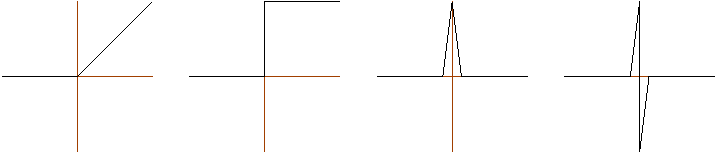
\includegraphics[width=\textwidth]{ode/inhomogeneous/delta}
  \end{center}
  \caption{The ramp function, the Heaviside function, the delta function, 
    and the derivative of the delta function.}
  \label{fig_delta}
\end{figure}



We write the differential equation for the Green function.
\[
G''(x|\xi) + p(x) G'(x|\xi) + q(x) G(x|\xi) = \delta(x-\xi)
\]
we see that only the $G''(x|\xi)$ term can have a delta function type 
singularity.  If one of the other terms had a delta function type singularity
then $G''(x|\xi)$ would be more singular than a delta function and there
would be nothing in the right hand side of the equation to match this 
kind of singularity.  
Analogous to the progression from a delta function to a Heaviside function
to a ramp function,
we see that $G'(x|\xi)$ will have a jump discontinuity and $G(x|\xi)$ will
be continuous.

Let $y_1$ and $y_2$ be two linearly independent solutions to the homogeneous
equation, $L[y] = 0$.  Since the Green function satisfies the 
homogeneous equation for $x \neq \xi$, it will be a linear combination of
the homogeneous solutions.
\[
G(x|\xi) = 
\begin{cases}
  c_1 y_1 + c_2 y_2 \quad &\mathrm{for}\ x < \xi \\
  d_1 y_1 + d_2 y_2 \quad &\mathrm{for}\ x > \xi
\end{cases}
\]

We require that $G(x|\xi)$ be continuous.
\begin{gather*}
  G(x|\xi)\big|_{x \to \xi^-} = G(x|\xi)\big|_{x \to \xi^+} 
  \\
  \intertext{We can write this in terms of the homogeneous solutions.}
  c_1 y_1(\xi) + c_2 y_2(\xi) = d_1 y_1(\xi) + d_2 y_2(\xi)
\end{gather*}

We integrate $L[G(x|\xi)] = \delta(x-\xi)$ from $\xi^-$ to $\xi+$.
\begin{gather*}
  \int_{\xi^-}^{\xi^+} \left[G''(x|\xi) + p(x)G'(x|\xi)+q(x)G(x|\xi) \right]\,\dd x = 
  \int_{\xi^-}^{\xi^+} \delta(x-\xi)\,\dd x. 
  \\
  \intertext{Since $G(x|\xi)$ is continuous and $G'(x|\xi)$ has only a 
    jump discontinuity two of the terms vanish.}
  \int_{\xi^-}^{\xi^+} p(x) G'(x|\xi)\,\dd x = 0 \qquad \mathrm{and} \qquad
  \int_{\xi^-}^{\xi^+} q(x) G(x|\xi)\,\dd x = 0
  \\
  \int_{\xi^-}^{\xi^+} G''(x|\xi)\,\dd x = \int_{\xi^-}^{\xi^+} \delta(x-\xi)\,\dd x 
  \\
  \big[ G'(x|\xi) \big]_{\xi^-}^{\xi^+}
  = \big[ H(x-\xi) \big]_{\xi^-}^{\xi^+} 
  \\
  G'(\xi^+|\xi) - G'(\xi^-|\xi) = 1
  \\
  \intertext{We write this jump condition in terms of the homogeneous 
    solutions.}
  d_1 y_1'(\xi) + d_2 y_2'(\xi) - c_1 y_1'(\xi) - c_2 y_2'(\xi) = 1
\end{gather*}
Combined with the two boundary conditions, this gives us a total of 
four equations to determine our four constants, $c_1$, $c_2$, $d_1$, and $d_2$.




\begin{Result}
  The second order inhomogeneous differential equation with homogeneous 
  boundary conditions
  \[ 
  L[y] = y'' + p(x)y' + q(x) y = f(x), \quad \mathrm{for}\ a < x < b, 
  \qquad B_1[y] = B_2[y] = 0,
  \]
  has the solution
  \[ 
  y = \int_a^b G(x|\xi)f(\xi)\,\dd \xi,
  \]
  where $G(x|\xi)$ satisfies the equation
  \[ 
  L[G(x|\xi)] = \delta(x-\xi), \quad \mathrm{for}\ a<x<b, \qquad
  B_1[G(x|\xi)] = B_2[G(x|\xi)] = 0.
  \]
  $G(x|\xi)$ is continuous and $G'(x|\xi)$ has a jump discontinuity of
  height $1$ at $x = \xi$.
\end{Result}






\begin{Example} \label{greens_fx}
  Solve the boundary value problem
  \[y'' = f(x), \qquad y(0) = y(1) = 0,\]
  using a Green function.

  A pair of solutions to the homogeneous equation are $y_1 = 1$ and $y_2 = x$.
  First note that only the trivial solution to the homogeneous equation
  satisfies the homogeneous boundary conditions.  Thus there is a unique solution
  to this problem.

  The Green function satisfies 
  \[ G''(x|\xi) = \delta(x-\xi), \qquad G(0|\xi) = G(1|\xi) = 0.\]
  The Green function has the form
  \[ G(x|\xi) = 
  \begin{cases}
    c_1 + c_2 x \quad &\mathrm{for}\ x < \xi \\
    d_1 + d_2 x \quad &\mathrm{for}\  x > \xi.
  \end{cases}
  \]
  Applying the two boundary conditions, we see that $c_1 = 0$ and $d_1=-d_2$.
  The Green function now has the form
  \[ G(x|\xi) = 
  \begin{cases}
    c x \quad &\mathrm{for}\  x < \xi \\
    d(x-1) \quad &\mathrm{for}\  x > \xi.
  \end{cases}
  \]
  Since the Green function must be continuous,
  \[ c \xi = d(\xi-1) \quad \to \quad d = c \frac{\xi}{\xi-1}.\]
  From the jump condition,
  \begin{gather*}
    \frac{\dd}{\dd x} c \frac{\xi}{\xi-1} (x-1) \Big|_{x=\xi} 
    - \frac{\dd}{\dd x} c x \Big|_{x=\xi} = 1 \\
    c \frac{\xi}{\xi-1} - c = 1 \\
    c = \xi-1.
  \end{gather*}
  Thus the Green function is
  \[ \boxed{ G(x|\xi) = 
    \begin{cases}
      (\xi-1) x \quad &\mathrm{for}\ x < \xi \\
      \xi(x-1) \quad &\mathrm{for}\ x > \xi.
    \end{cases} }
  \]
  The Green function is plotted in Figure~\ref{greens_x} for various values
  of $\xi$.  We show $G(x|0.05)$, $G(x|0.25)$, $G(x|0.5)$ and $G(x|0.75)$.
  The solution to $y'' = f(x)$ is

  \[ y(x) = \int_0^1 G(x|\xi) f(\xi)\,\dd \xi \]
  \[ \boxed{ y(x) = (x-1) \int_0^x \xi f(\xi)\,\dd \xi 
    + x \int_x^1 (\xi - 1) f(\xi)\,\dd \xi. } \]

  \begin{figure}[tb!]
    \begin{center}
      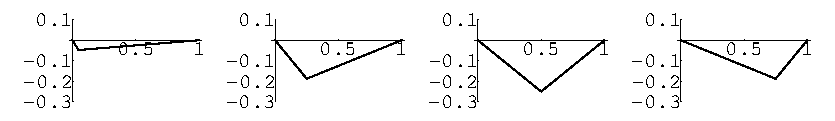
\includegraphics[width=\textwidth]{ode/inhomogeneous/greensx}
    \end{center}
    \caption{Plots of the Green functions.} 
    \label{greens_x}
  \end{figure}

\end{Example}














\begin{Example}
  Solve the boundary value problem
  \[ 
  y'' = f(x), \qquad y(0) = 1, \quad y(1) = 2.
  \]

  In Example~\ref{greens_fx} we saw that the solution to
  \[ 
  u'' = f(x), \qquad u(0) = u(1) = 0 
  \]
  is
  \[ 
  u(x) = (x-1) \int_0^x \xi f(\xi)\,\dd \xi + x \int_x^1 (\xi - 1) f(\xi)\,\dd \xi.
  \]

  Now we have to find the solution to
  \[ 
  v'' = 0, \qquad v(0) = 1, \quad u(1) = 2.
  \]
  The general solution is
  \[ 
  v = c_1 + c_2 x.
  \]
  Applying the boundary conditions yields
  \[ 
  v = 1 + x.
  \]

  Thus the solution for $y$ is
  \[ 
  \boxed{
    y = 1 + x + (x-1) \int_0^x \xi f(\xi)\,\dd \xi 
    + x \int_x^1 (\xi - 1) f(\ xi)\,\dd \xi.
    }
  \]
\end{Example}

















\begin{Example}
  Consider
  \[ 
  y'' = x, \qquad y(0) = y(1) = 0. 
  \]

  \paragraph{Method 1.}
  Integrating the differential equation twice yields
  \[ 
  y = \frac{1}{6} x^3 + c_1 x + c_2. 
  \]
  Applying the boundary conditions, we find that the solution is
  \[ 
  \boxed{ 
    y = \frac{1}{6} (x^3 - x). 
    } 
  \]

  \paragraph{Method 2.}
  Using the Green function to find the solution,
  \begin{align*}
    y       &= (x-1) \int_0^x \xi^2 \,\dd \xi + x \int_x^1 (\xi-1)\xi\,\dd \xi \\
    &= (x-1) \frac{1}{3} x^3 + x \left( \frac{1}{3} - \frac{1}{2}
      -\frac{1}{3} x^3 + \frac{1}{2} x^2 \right)
  \end{align*}
  \[ 
  \boxed{ 
    y = \frac{1}{6} (x^3 - x). 
    } 
  \]
\end{Example}














\begin{Example} \label{greens_sinx}
  Find the solution to the differential equation
  \[ 
  y'' - y = \sin x, 
  \]
  that is bounded for all $x$.

  The Green function for this problem satisfies
  \[
  G''(x|\xi) - G(x|\xi) = \delta(x-\xi).
  \]
  The homogeneous solutions are $y_1 = \e^x$, and $y_2 = \e^{-x}$.
  The Green function has the form
  \[ 
  G(x|\xi) = 
  \begin{cases}
    c_1 \e^x + c_2 \e^{-x} \quad &\mathrm{for}\ x < \xi \\
    d_1 \e^x + d_2 \e^{-x} \quad &\mathrm{for}\ x > \xi. 
  \end{cases}
  \]
  Since the solution must be bounded for all $x$, the Green function must
  also be bounded.  Thus $c_2 = d_1 = 0$.  
  The Green function now has the form
  \[ 
  G(x|\xi) = 
  \begin{cases}
    c \e^x \quad &\mathrm{for}\ x < \xi \\
    d \e^{-x} \quad &\mathrm{for}\ x > \xi. 
  \end{cases}
  \]
  Requiring that $G(x|\xi)$ be continuous gives us the condition
  \[ 
  c \e^\xi = d \e^{-\xi} \quad \to \quad d = c \e^{2\xi}.
  \]
  $G(x|\xi)$ has a jump discontinuity of height $1$ at $x = \xi$.
  \begin{gather*}
    \frac{\dd}{\dd x}c \e^{2\xi} \e^{-x}\bigg|_{x=\xi} 
    - \frac{\dd}{\dd x} c \e^x\bigg|_{x=\xi} = 1 \\
    -c \e^{2\xi} \e^{-\xi} - c \e^\xi = 1 \\
    c = -\frac{1}{2} \e^{-\xi}
  \end{gather*}
  The Green function is then
  \[ 
  G(x|\xi) = 
  \begin{cases}
    -\frac{1}{2} \e^{x-\xi} \quad &\mathrm{for}\ x < \xi \\
    -\frac{1}{2} \e^{-x+\xi} \quad &\mathrm{for}\ x > \xi 
  \end{cases} 
  \]
  \[ 
  \boxed{ 
    G(x|\xi) = -\frac{1}{2} \e^{-|x-\xi|}. 
    } 
  \]
  A plot of $G(x|0)$ is given in Figure~\ref{greens_ex}. 
  The solution to $y'' - y = \sin x$ is
  \begin{align*}
    y(x) &= \int_{-\infty}^\infty -\frac{1}{2} \e^{-|x-\xi|} \sin\xi\,\dd \xi \\
    &= -\frac{1}{2} \left( \int_{-\infty}^x \sin\xi \e^{x-\xi}\,\dd \xi + 
      \int_x^\infty \sin\xi \e^{-x+\xi}\,\dd \xi \right) \\
    &= -\frac{1}{2} (-\frac{\sin x+\cos x}{2} +\frac{-\sin x+\cos x}{2})
  \end{align*}
  \[ 
  \boxed{ 
    y = \frac{1}{2} \sin x. 
    } 
  \]
  \begin{figure}[tb!]
    \begin{center}
      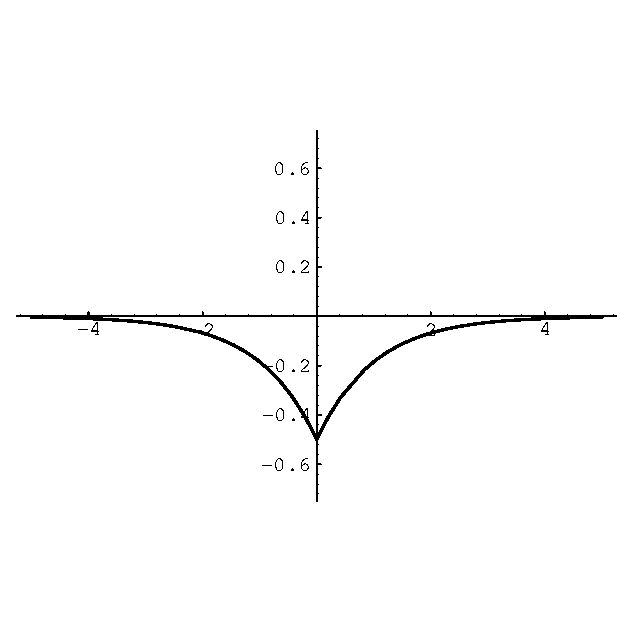
\includegraphics[width=0.5\textwidth]{ode/inhomogeneous/greens1}
    \end{center}
    \caption{Plot of the Green function.} 
    \label{greens_ex}
  \end{figure}

\end{Example}






%%-------------------------------------------------------------------------
\subsection{Green Functions for Sturm-Liouville Problems}



Consider the problem
\begin{gather*}
  L[y] = \left( p(x) y' \right)' + q(x) y = f(x), 
  \quad \mathrm{subject to}
  \\
  B_1[y] = \alpha_1 y(a) + \alpha_2 y'(a) = 0, \quad
  B_2[y] = \beta_1 y(b) + \beta_2 y'(b) = 0. 
\end{gather*}
This is known as a Sturm-Liouville problem.  Equations of this type
often occur when solving partial differential equations.
The Green function associated with this problem satisfies
\[ 
L[G(x|\xi)] = \delta(x-\xi), \quad B_1[G(x|\xi)] = B_2[G(x|\xi)] = 0.
\]
Let $y_1$ and $y_2$ be two non-trivial homogeneous solutions that satisfy
the left and right boundary conditions, respectively.
\[ 
L[y_1] = 0, \quad B_1[y_1] = 0, \qquad L[y_2] = 0, \quad B_2[y_2] = 0. 
\]
The Green function satisfies the homogeneous equation for $x \neq \xi$ 
and satisfies the homogeneous boundary conditions.
Thus it must have the following form.
\[ 
G(x|\xi) = 
\begin{cases}
  c_1(\xi) y_1(x) \quad &\mathrm{for}\ a \leq x \leq \xi, \\
  c_2(\xi) y_2(x) \quad &\mathrm{for}\ \xi \leq x \leq b,
\end{cases}
\]
Here $c_1$ and $c_2$ are unknown functions of $\xi$.

The first constraint on $c_1$ and $c_2$ comes from the continuity condition.
\begin{gather*}
  G(\xi^-|\xi) = G(\xi^+|\xi)
  \\
  c_1(\xi) y_1(\xi) = c_2(\xi) y_2(\xi)
\end{gather*}
We write the inhomogeneous equation in the standard form.
\[ 
G''(x|\xi) + \frac{p'}{p} G'(x|\xi) + \frac{q}{p} G(x|\xi) = \frac{\delta(x-\xi)}{p}
\]
The second constraint on $c_1$ and $c_2$ comes from the jump condition.
\begin{gather*}
  G'(\xi^+|\xi) -  G'(\xi^-|\xi) = \frac{1}{p(\xi)} 
  \\
  c_2(\xi) y_2'(\xi) - c_1(\xi) y_1'(\xi) = \frac{1}{p(\xi)}
\end{gather*}
Now we have a system of equations to determine $c_1$ and $c_2$.
\begin{align*}
  c_1(\xi) y_1(\xi) - c_2(\xi) y_2(\xi) &= 0 
  \\
  c_1(\xi) y_1'(\xi) - c_2(\xi) y_2'(\xi) &= -\frac{1}{p(\xi)}
\end{align*}
We solve this system with Kramer's rule.
\[ 
c_1(\xi) = -\frac{y_2(\xi)}{p(\xi) (-W(\xi))}, \quad
c_2(\xi) = - \frac{y_1(\xi)}{p(\xi) (-W(\xi))}
\]
Here $W(x)$ is the Wronskian of $y_1(x)$ and $y_2(x)$.  
The Green function is
\[ 
\boxed{ 
  G(x|\xi) = 
  \begin{cases}
    \frac{y_1(x) y_2(\xi)}{p(\xi) W(\xi)} \quad &\mathrm{for}\ a \leq x \leq \xi, 
    \\
    \frac{y_2(x) y_1(\xi)}{p(\xi) W(\xi)} \quad &\mathrm{for}\ \xi \leq x \leq b.
  \end{cases} 
  }
\]
The solution of the Sturm-Liouville problem is 
\[
y = \int_a^b G(x|\xi) f(\xi) \,\dd \xi.
\]



\begin{Result}
  The problem
  \begin{gather*}
    L[y] = \left( p(x) y' \right)' + q(x) y = f(x), 
    \quad \mathrm{subject to}
    \\
    B_1[y] = \alpha_1 y(a) + \alpha_2 y'(a) = 0, \quad
    B_2[y] = \beta_1 y(b) + \beta_2 y'(b) = 0. 
  \end{gather*}
  has the Green function
  \[ 
  G(x|\xi) = 
  \begin{cases}
    \frac{y_1(x) y_2(\xi)}{p(\xi) W(\xi)} \quad &\mathrm{for}\ a \leq x \leq \xi, 
    \\
    \frac{y_2(x) y_1(\xi)}{p(\xi) W(\xi)} \quad &\mathrm{for}\ \xi \leq x \leq b,
  \end{cases} 
  \]
  where $y_1$ and $y_2$ are non-trivial homogeneous solutions that satisfy
  $B_1[y_1] = B_2[y_2] = 0$, and $W(x)$ is the Wronskian of $y_1$ and $y_2$.
\end{Result}








\begin{Example}
  Consider the equation
  \[ 
  y'' - y = f(x), \qquad y(0) = y(1) = 0.
  \]
  A set of solutions to the homogeneous equation is $\{ \e^x, \e^{-x} \}$.  
  Equivalently, one could use the set $\{ \cosh x, \sinh x \}$.
  Note that $\sinh x$ satisfies the left boundary condition and $\sinh (x-1)$
  satisfies the right boundary condition.
  The Wronskian of these two homogeneous solutions is
  \begin{align*}
    W(x)    
    &= \begin{vmatrix}
      \sinh x         &       \sinh (x-1)     \\
      \cosh x         &       \cosh(x-1)
    \end{vmatrix} 
    \\
    &= \sinh x \cosh(x-1) - \cosh x \sinh(x-1) 
    \\
    &= \frac{1}{2} [\sinh (2x-1) + \sinh (1) ]
    - \frac{1}{2} [\sinh (2x-1) - \sinh(1)] 
    \\
    &= \sinh (1).
  \end{align*}
  The Green function for the problem is then
  \[ 
  \boxed{ 
    G(x|\xi) = 
    \begin{cases}
      \frac{\sinh x \sinh(\xi-1)}{\sinh(1)} \quad &\mathrm{for}\ 0 \leq x \leq \xi \\
      \frac{\sinh(x-1) \sinh \xi}{\sinh(1)} \quad &\mathrm{for}\ \xi \leq x \leq 1.
    \end{cases} 
    } 
  \]
  The solution to the problem is
  \[ 
  \boxed{ 
    y = \frac{\sinh(x-1)}{\sinh(1)} \int_0^x \sinh(\xi) f(\xi)\,\dd \xi
    + \frac{\sinh(x)}{\sinh(1)} \int_x^1 \sinh(\xi-1) f(\xi)\,\dd \xi . 
    } 
  \]
\end{Example}




















%%-----------------------------------------------------------------------------
\subsection{Initial Value Problems}
Consider 
\[
L[y] = y'' + p(x) y' + q(x) y = f(x), \quad \mathrm{for}\ a < x < b,
\]
subject the the initial conditions
\[
y(a) = \gamma_1, \qquad y'(a) = \gamma_2.
\]
The solution is $y = u + v$ where
\[
u'' + p(x) u' + q(x) u = f(x), \qquad u(a) = 0, \quad u'(a) = 0,
\]
and
\[
v'' + p(x) v' + q(x) v = 0, \qquad v(a) = \gamma_1, \quad v'(a) = \gamma_2.
\]
Since the Wronskian
\[
W(x) = c \exp\left(-\int p(x)\,\dd x \right)
\]
is non-vanishing, the solutions of the differential equation for $v$ are 
linearly independent.  Thus there is a unique solution for $v$ that 
satisfies the initial conditions.

The Green function for $u$ satisfies
\[
G''(x|\xi) + p(x) G'(x|\xi) + q(x) G(x|\xi) = \delta(x-\xi), \qquad
G(a|\xi) = 0, \quad G'(a|\xi) = 0.
\]
The continuity and jump conditions are
\[
G(\xi^-|\xi) = G(\xi^+|\xi), \qquad G'(\xi^-|\xi) + 1 = G'(\xi^+|\xi).
\]
Let $u_1$ and $u_2$ be two linearly independent solutions of the 
differential equation.  For $x<\xi$, $G(x|\xi)$ is a linear combination 
of these solutions.  Since the Wronskian is non-vanishing, only the
trivial solution satisfies the homogeneous initial conditions.  The Green
function must be
\[
G(x|\xi) = 
\begin{cases}
  0 \quad &\mathrm{for}\ x < \xi \\
  u_\xi(x) \quad &\mathrm{for}\ x > \xi,
\end{cases}
\]
where $u_\xi(x)$ is the linear combination of $u_1$ and $u_2$ that satisfies
\[
u_\xi(\xi) = 0, \qquad u_\xi'(\xi) = 1.
\]
Note that the non-vanishing Wronskian ensures a unique solution for $u_\xi$.
We can write the Green function in the form
\[
G(x|\xi) = H(x-\xi) u_\xi(x).
\]
This is known as the \textbf{causal solution}.
The solution for $u$ is
\begin{align*}
  u       &= \int_a^b G(x|\xi) f(\xi) \,\dd \xi \\
  &= \int_a^b H(x-\xi) u_\xi(x) f(\xi) \,\dd \xi \\
  &= \int_a^x u_\xi(x) f(\xi) \,\dd \xi 
\end{align*}

Now we have the solution for $y$,
\[
y = v + \int_a^x u_\xi(x) f(\xi) \,\dd \xi.
\]



\begin{Result}
  The solution of the problem
  \[
  y'' + p(x) y' + q(x) y = f(x), \qquad y(a) = \gamma_1, \quad y'(a) = \gamma_2,
  \]
  is
  \[
  y = y_h + \int_a^x y_\xi(x) f(\xi) \,\dd \xi
  \]
  where $y_h$ is the combination of the homogeneous solutions of the equation 
  that satisfy the initial conditions and $y_\xi(x)$ is the linear combination
  of homogeneous solutions that satisfy $y_\xi(\xi) = 0$,
  $y_\xi'(\xi) = 1$.
\end{Result}










%%-----------------------------------------------------------------------------
\subsection{Problems with Unmixed Boundary Conditions}

Consider 
\[
L[y] = y'' + p(x) y' + q(x) y = f(x), \quad \mathrm{for}\ a < x < b,
\]
subject the the unmixed boundary conditions
\[
\alpha_1 y(a) + \alpha_2 y'(a) = \gamma_1, \qquad 
\beta_1 y(b) + \beta_2 y'(b) = \gamma_2.
\]
The solution is $y = u + v$ where
\[
u'' + p(x) u' + q(x) u = f(x), \qquad \alpha_1 u(a) + \alpha_2 u'(a) = 0, 
\quad \beta_1 u(b) + \beta_2 u'(b) = 0,
\]
and
\[
v'' + p(x) v' + q(x) v = 0, \qquad \alpha_1 v(a) + \alpha_2 v'(a) = \gamma_1, 
\quad \beta_1 v(b) + \beta_2 v'(b) = \gamma_2.
\]
The problem for $v$ may have no solution, a unique solution or an infinite
number of solutions.  We consider only the case that there is a unique solution
for $v$.  In this case the homogeneous equation subject to homogeneous
boundary conditions has only the trivial solution.

The Green function for $u$ satisfies
\[
G''(x|\xi) + p(x) G'(x|\xi) + q(x) G(x|\xi) = \delta(x-\xi), 
\]
\[
\alpha_1 G(a|\xi) + \alpha_2 G'(a|\xi) = 0, \quad 
\beta_1 G(b|\xi) + \beta_2 G'(b|\xi) = 0.
\]
The continuity and jump conditions are
\[
G(\xi^-|\xi) = G(\xi^+|\xi), \qquad G'(\xi^-|\xi) + 1 = G'(\xi^+|\xi).
\]
Let $u_1$ and $u_2$ be two solutions of the homogeneous equation that satisfy
the left and right boundary conditions, respectively.  The non-vanishing 
of the Wronskian ensures that these solutions exist.  Let $W(x)$ denote
the Wronskian of $u_1$ and $u_2$.  Since the homogeneous equation with 
homogeneous boundary conditions has only the trivial solution, $W(x)$ is
nonzero on $[a,b]$.  The Green function has the form
\[
G(x|\xi) = 
\begin{cases}
  c_1 u_1 \quad &\mathrm{for}\ x < \xi, \\
  c_2 u_2 \quad &\mathrm{for}\ x > \xi.
\end{cases}
\]
The continuity and jump conditions for Green function gives us the 
equations
\begin{align*}
  c_1 u_1(\xi) - c_2 u_2(\xi) &= 0 \\
  c_1 u_1'(\xi) - c_2 u_2'(\xi) &= -1.
\end{align*}
Using Kramer's rule, the solution is
\[
c_1 = \frac{u_2(\xi)}{W(\xi)}, \qquad
c_2 = \frac{u_1(\xi)}{W(\xi)}.
\]
Thus the Green function is
\[
G(x|\xi) = 
\begin{cases}
  \frac{u_1(x) u_2(\xi)}{W(\xi)} \quad &\mathrm{for}\ x < \xi, \\
  \frac{u_1(\xi) u_2(x)}{W(\xi)} \quad &\mathrm{for}\ x > \xi.
\end{cases}
\]
The solution for $u$ is
\[
u = \int_a^b G(x|\xi) f(\xi) \,\dd \xi.
\]
Thus if there is a unique solution for $v$, the solution for $y$ is
\[
y = v + \int_a^b G(x|\xi) f(\xi) \,\dd \xi.
\]




\begin{Result}
  Consider the problem
  \[
  y'' + p(x) y' + q(x) y = f(x), 
  \]
  \[
  \alpha_1 y(a) + \alpha_2 y'(a) = \gamma_1, \qquad
  \beta_1 y(b) + \beta_2 y'(b) = \gamma_2.
  \]
  If the homogeneous differential equation subject to the inhomogeneous 
  boundary conditions has the unique solution $y_h$, then the problem has 
  the unique solution
  \[
  y = y_h + \int_a^b G(x|\xi) f(\xi) \,\dd \xi
  \]
  where 
  \[
  G(x|\xi) =
  \begin{cases}
    \frac{u_1(x) u_2(\xi)}{W(\xi)} \quad &\mathrm{for}\ x < \xi, \\
    \frac{u_1(\xi) u_2(x)}{W(\xi)} \quad &\mathrm{for}\ x > \xi,
  \end{cases}
  \]
  $u_1$ and $u_2$ are solutions of the homogeneous differential equation that
  satisfy the left and right boundary conditions, respectively, and
  $W(x)$ is the Wronskian of $u_1$ and $u_2$.
\end{Result}











%%-----------------------------------------------------------------------------
\subsection{Problems with Mixed Boundary Conditions}

Consider 
\[
L[y] = y'' + p(x) y' + q(x) y = f(x), \quad \mathrm{for}\ a < x < b,
\]
subject the the mixed boundary conditions
\[
B_1[y] = \alpha_{11} y(a) + \alpha_{12} y'(a) 
+ \beta_{11} y(b) + \beta_{12} y'(b) = \gamma_1, 
\]
\[
B_2[y] = \alpha_{21} y(a) + \alpha_{22} y'(a) 
+ \beta_{21} y(b) + \beta_{22} y'(b) = \gamma_2. 
\]
The solution is $y = u + v$ where
\[
u'' + p(x) u' + q(x) u = f(x), \qquad B_1[u] = 0, 
\quad B_2[u] = 0,
\]
and
\[
v'' + p(x) v' + q(x) v = 0, \qquad B_1[v] = \gamma_1, 
\quad B_2[v] = \gamma_2.
\]

The problem for $v$ may have no solution, a unique solution or an infinite
number of solutions.  Again we consider only the case that there is a unique 
solution for $v$.  In this case the homogeneous equation subject to homogeneous
boundary conditions has only the trivial solution.

Let $y_1$ and $y_2$ be two solutions of the homogeneous equation that satisfy
the boundary conditions $B_1[y_1] = 0$ and $B_2[y_2] = 0$.  Since the 
completely homogeneous problem has no solutions, we know that 
$B_1[y_2]$ and $B_2[y_1]$ are nonzero.  The solution for $v$ has the form
\[
v = c_1 y_1 + c_2 y_2.
\]
Applying the two boundary conditions yields
\[
v = \frac{\gamma_2}{B_2[y_1]} y_1 + \frac{\gamma_1}{B_1[y_2]} y_2.
\]

The Green function for $u$ satisfies
\[
G''(x|\xi) + p(x) G'(x|\xi) + q(x) G(x|\xi) = \delta(x-\xi), \qquad
B_1[G] = 0, \quad B_2[G] = 0.
\]
The continuity and jump conditions are
\[
G(\xi^-|\xi) = G(\xi^+|\xi), \qquad G'(\xi^-|\xi) + 1 = G'(\xi^+|\xi).
\]
We write the Green function as the sum of the causal
solution and the two homogeneous solutions
\[
G(x|\xi) = H(x-\xi) y_\xi(x) + c_1 y_1(x) + c_2 y_2(x)
\]
With this form, the continuity and jump conditions are automatically 
satisfied.  Applying the boundary conditions yields
\begin{align*}
  B_1[G] &= B_1[H(x-\xi)y_\xi] + c_2 B_1[y_2] = 0, \\
  B_2[G] &= B_2[H(x-\xi)y_\xi] + c_1 B_2[y_1] = 0,
\end{align*}
\begin{align*}
  B_1[G] &= \beta_{11} y_\xi(b) + \beta_{12} y_\xi'(b) + c_2 B_1[y_2] = 0, \\
  B_2[G] &= \beta_{21} y_\xi(b) + \beta_{22} y_\xi'(b) + c_1 B_2[y_1] = 0,
\end{align*}
\[
G(x|\xi) = H(x-\xi) y_\xi(x) 
- \frac{\beta_{21} y_\xi(b) + \beta_{22} y_\xi'(b)}{B_2[y_1]} y_1(x) 
- \frac{\beta_{11} y_\xi(b) + \beta_{12} y_\xi'(b)}{B_1[y_2]} y_2(x).
\]
Note that the Green function is well defined since $B_2[y_1]$ and 
$B_1[y_2]$ are nonzero.  The solution for $u$ is
\[
u = \int_a^b G(x|\xi) f(\xi) \,\dd \xi.
\]
Thus if there is a unique solution for $v$, the solution for $y$ is
\[
y = \int_a^b G(x|\xi) f(\xi) \,\dd \xi + \frac{\gamma_2}{B_2[y_1]} y_1 
+ \frac{\gamma_1}{B_1[y_2]} y_2.
\]




\begin{Result}
  Consider the problem
  \[
  y'' + p(x) y' + q(x) y = f(x), 
  \]
  \[
  B_1[y] = \alpha_{11} y(a) + \alpha_{12} y'(a)
  + \beta_{11} y(b) + \beta_{12} y'(b) = \gamma_1, 
  \]
  \[
  B_2[y] = \alpha_{21} y(a) + \alpha_{22} y'(a)
  + \beta_{21} y(b) + \beta_{22} y'(b) = \gamma_2.
  \]
  If the homogeneous differential equation subject to the homogeneous 
  boundary conditions has no solution, then the problem has 
  the unique solution
  \[
  y = \int_a^b G(x|\xi) f(\xi) \,\dd \xi + \frac{\gamma_2}{B_2[y_1]} y_1
  + \frac{\gamma_1}{B_1[y_2]} y_2,
  \]
  where 
  \begin{multline*}
    G(x|\xi) = H(x-\xi) y_\xi(x)
    - \frac{\beta_{21} y_\xi(b) + \beta_{22} y_\xi'(b)}{B_2[y_1]} y_1(x) \\
    - \frac{\beta_{11} y_\xi(b) + \beta_{12} y_\xi'(b)}{B_1[y_2]} y_2(x),
  \end{multline*}
  $y_1$ and $y_2$ are solutions of the homogeneous differential equation that
  satisfy the first and second boundary conditions, respectively, and 
  $y_\xi(x)$ is the solution of the homogeneous equation that satisfies
  $y_\xi(\xi) = 0$, $y_\xi'(\xi) = 1$.
\end{Result}




%%=============================================================================
\section{Green Functions for Higher Order Problems}

Consider the $n_{t h}$ order differential equation
\[
L[y] = y^{(n)} + p_{n-1}(x) y^{(n-1)} + \cdots + p_1(x) y' + p_0 y = f(x)
\quad \mathrm{on}\ a < x < b,
\]
subject to the $n$ independent boundary conditions
\[
B_j[y] = \gamma_j
\]
where the boundary conditions are of the form
\[
B[y] \equiv \sum_{k=0}^{n-1} \alpha_k y^{(k)}(a) 
+ \sum_{k=0}^{n-1} \beta_k y^{(k)}(b).
\]
We assume that the coefficient functions in the differential equation 
are continuous on $[a,b]$.
The solution is $y = u + v$ where $u$ and $v$ satisfy
\[
L[u] = f(x), \quad \mathrm{with} \quad B_j[u] = 0,
\]
and
\[
L[v] = 0, \quad \mathrm{with} \quad B_j[v] = \gamma_j
\]

From Result~\ref{ioeostie}, we know that if the completely homogeneous problem
\[
L[w] = 0, \quad \mathrm{with} \quad B_j[w] = 0,
\]
has only the trivial solution, then the solution for $y$ exists and is 
unique.  We will construct this solution using Green functions.




First we consider the problem for $v$.
Let $\{y_1,\ldots,y_n\}$ be a set of linearly
independent solutions.  The solution for $v$ has the form
\[
v = c_1 y_1 + \cdots + c_n y_n
\]
where the constants are determined by the matrix equation
\[
\begin{pmatrix}
  B_1[y_1] & B_1[y_2] & \cdots & B_1[y_n] \\
  B_2[y_1] & B_2[y_2] & \cdots & B_2[y_n] \\
  \vdots   & \vdots   & \ddots & \vdots   \\
  B_n[y_1] & B_n[y_2] & \cdots & B_n[y_n]
\end{pmatrix}
\
\begin{pmatrix}
  c_1 \\
  c_2 \\
  \vdots \\
  c_n
\end{pmatrix}
=
\begin{pmatrix}
  \gamma_1  \\
  \gamma_2  \\
  \vdots \\
  \gamma_n 
\end{pmatrix}.
\]


To solve the problem for $u$ we consider the Green function satisfying
\[
L[G(x|\xi)] = \delta(x-\xi), \quad \mathrm{with} \quad B_j[G] = 0.
\]
Let $y_\xi(x)$ be the linear combination of the homogeneous solutions that
satisfy the conditions
\begin{align*}
  y_\xi(\xi) &= 0 \\
  y_\xi'(\xi) &= 0 \\
  \vdots \ \ &= \vdots \\
  y_\xi^{(n-2)}(\xi) &= 0 \\
  y_\xi^{(n-1)}(\xi) &= 1.
\end{align*}
The causal solution is then
\[
y_c(x) = H(x-\xi) y_\xi(x).
\]
The Green function has the form
\[
G(x|\xi) = H(x-\xi) y_\xi(x) + d_1 y_1(x) + \cdots + d_n y_n(x)
\]
The constants are determined by the matrix equation
\[
\begin{pmatrix}
  B_1[y_1] & B_1[y_2] & \cdots & B_1[y_n] \\
  B_2[y_1] & B_2[y_2] & \cdots & B_2[y_n] \\
  \vdots   & \vdots   & \ddots & \vdots   \\
  B_n[y_1] & B_n[y_2] & \cdots & B_n[y_n]
\end{pmatrix}
\
\begin{pmatrix}
  d_1 \\
  d_2 \\
  \vdots \\
  d_n
\end{pmatrix}
=
\begin{pmatrix}
  -B_1[H(x-\xi) y_\xi(x)] \\
  -B_2[H(x-\xi) y_\xi(x)] \\
  \vdots \\
  -B_n[H(x-\xi) y_\xi(x)] \\
\end{pmatrix}.
\]
The solution for $u$ then is
\[
u = \int_a^b G(x|\xi) f(\xi) \,\dd \xi.
\]



\begin{Result}
  Consider the $n_{t h}$ order differential equation
  \[
  L[y] = y^{(n)} + p_{n-1}(x) y^{(n-1)} + \cdots + p_1(x) y' + p_0 y = f(x)
  \quad \mathrm{on}\ a < x < b,
  \]
  subject to the $n$ independent boundary conditions
  \[
  B_j[y] = \gamma_j
  \]
  If the homogeneous differential equation subject to the homogeneous 
  boundary conditions has only the trivial solution, then the problem has 
  the unique solution
  \[
  y = \int_a^b G(x|\xi) f(\xi) \,\dd \xi + c_1 y_1 + \cdots c_n y_n
  \]
  where 
  \[
  G(x|\xi) = H(x-\xi) y_\xi(x) + d_1 y_1(x) + \cdots + d_n y_n(x),
  \]
  $\{y_1,\ldots,y_n\}$ is a set of solutions of the homogeneous 
  differential equation, and the constants $c_j$ and $d_j$ can be determined
  by solving sets of linear equations.
\end{Result}




















\begin{Example}
  Consider the problem
  \[
  y'''-y''+y'-y=f(x),
  \]
  \[
  y(0)=1, \quad y'(0)=2, \quad y(1)=3.
  \]

  The completely homogeneous associated problem is
  \[
  w'''-w''+w'-w=0, \quad w(0)= w'(0)= w(1)=0.
  \]
  The solution of the differential equation is
  \[
  w = c_1 \cos x + c_2 \sin x + c_2 \e^x.
  \]
  The boundary conditions give us the equation
  \[
  \begin{pmatrix}
    1 & 0 & 1 \\
    0 & 1 & 1 \\
    \cos 1 & \sin 1 & e
  \end{pmatrix}
  \begin{pmatrix}
    c_1 \\
    c_2 \\
    c_3
  \end{pmatrix}
  =
  \begin{pmatrix}
    0 \\ 
    0 \\
    0
  \end{pmatrix}.
  \]
  The determinant of the matrix is $e-\cos 1-\sin 1 \neq 0$.  
  Thus the homogeneous problem has only the trivial solution and the 
  inhomogeneous problem has a unique solution.

  We separate the inhomogeneous problem into the two problems
  \[
  u'''-u''+u'-u=f(x),\quad u(0)=u'(0)=u(1)=0,
  \]
  \[
  v'''-v''+v'-v=0,\quad v(0)=1, \quad v'(0)=2, \quad v(1)=3,
  \]

  First we solve the problem for $v$.  The solution of the differential equation
  is
  \[
  v = c_1 \cos x + c_2 \sin x + c_2 \e^x.
  \]
  The boundary conditions yields the equation
  \[
  \begin{pmatrix}
    1 & 0 & 1 \\
    0 & 1 & 1 \\
    \cos 1 & \sin 1 & e
  \end{pmatrix}
  \begin{pmatrix}
    c_1 \\
    c_2 \\
    c_3
  \end{pmatrix}
  =
  \begin{pmatrix}
    1 \\ 
    2 \\
    3
  \end{pmatrix}.
  \]
  The solution for $v$ is
  \[
  v = \frac{1}{e - \cos 1 - \sin 1} \big[ (e+\sin 1 - 3)\cos x 
  + (2e - \cos 1 - 3) \sin x + (3 - \cos 1 - 2 \sin 1) \e^x \big].
  \]



  Now we find the Green function for the problem in $u$.  The causal 
  solution is
  \[
  H(x-\xi)u_\xi(x) = H(x-\xi) \frac{1}{2} \big[ (\sin\xi-\cos\xi)\cos x
  - (\sin\xi+\cos\xi)\sin\xi + \e^{-\xi} \e^x \big],
  \]
  \[
  H(x-\xi)u_\xi(x) = 
  \frac{1}{2} H(x-\xi) \big[ \e^{x-\xi} - \cos(x-\xi) - \sin(x-\xi) \big].
  \]
  The Green function has the form
  \[
  G(x|\xi) = H(x-\xi)u_\xi(x) + c_1 \cos x + c_2 \sin x + c_3 \e^x.
  \]
  The constants are determined by the three conditions
  \begin{align*}
    &\big[c_1 \cos x + c_2 \sin x + c_3 \e^x \big]_{x=0} = 0, \\
    &\left[\frac{\partial}{\partial x}\left(c_1 \cos x + c_2 \sin x + c_3 \e^x \right)
    \right]_{x=0} = 0, \\
    &\big[u_\xi(x) + c_1 \cos x + c_2 \sin x + c_3 \e^x \big]_{x=1} = 0. 
  \end{align*}
  The Green function is
  \[
  G(x|\xi)=\frac{1}{2} H(x-\xi) \big[ \e^{x-\xi} - \cos(x-\xi) - \sin(x-\xi) \big]
  + \frac{\cos(1-\xi)+\sin(1-\xi)-\e^{1-\xi}}{2(\cos 1 + \sin 1 - e)}
  \big[ \cos x + \sin x - \e^x \big]
  \]
  The solution for $v$ is 
  \[
  v = \int_0^1 G(x|\xi) f(\xi) \,\dd \xi.
  \]


  Thus the solution for $y$ is

  \begin{center}
    \fbox{
      \parbox{5.5in}{
        \begin{multline*}
          y = \int_0^1 G(x|\xi) f(\xi) \,\dd \xi
          + \frac{1}{e - \cos 1 - \sin 1} \big[ (e+\sin 1 - 3)\cos x \\
          + (2e - \cos 1 - 3) \sin x + (3 - \cos 1 - 2 \sin 1) \e^x \big].
        \end{multline*}
        }
      }
  \end{center}
\end{Example}











%%============================================================================
\section{Fredholm Alternative Theorem}
\index{Fredholm alternative theorem}
\index{boundary value problems}

\paragraph{Orthogonality.}
Two real vectors, $u$ and $v$ are orthogonal if $u \cdot v = 0$.  
Consider two functions, $u(x)$ and $v(x)$, defined in $[a,b]$.
The dot product in vector space is analogous to the integral
\[
\int_a^b u(x) v(x) \,\dd x
\]
in function space.  Thus two real functions are orthogonal if
\[
\int_a^b u(x) v(x) \,\dd x = 0.
\]




Consider the $n^{t h}$ order linear inhomogeneous differential equation
\[ L[y] = f(x) \quad \mathrm{on}\ [a,b],\]
subject to the linear inhomogeneous boundary conditions
\[ B_j[y] = 0, \quad \mathrm{for}\ j = 1, 2, \ldots n.\]


The Fredholm alternative theorem tells us if the problem has a unique solution,
an infinite number of solutions, or no solution.  Before presenting the
theorem, we will consider a few motivating examples.



%%\begin{Example}
%%\label{fred1}
%%Consider the problem
%%\[
%%y''=1, \qquad y(0)=0, \quad y(1)=0.
%%\]
%%The general solution is
%%\[
%%y = \frac{x^2}{2} + c_1 + c_2 x.
%%\]
%%Applying the boundary conditions, the unique solution of the problem is
%%\[
%%y = \frac{1}{2}(x^2 - x).
%%\]
%%\end{Example}









%%\begin{Example}
%%\label{fred2}
%%Consider the problem
%%\[
%%y''=1, \qquad y'(0)=0, \quad y'(1)=0.
%%\]
%%The general solution is
%%\[
%%y = \frac{x^2}{2} + c_1 + c_2 x.
%%\]
%%Applying the boundary conditions,
%%\begin{alignat*}{2}
%%y'(0) &= 0 \quad &\to \quad c_2 &= 0 \\
%%y'(1) &= 0 \quad &\to \quad 1 &= 0.
%%\end{alignat*}
%%Since this equation is inconsistent, the problem has no solution.
%%\end{Example}



%%Note that in Example~\ref{fred1} the homogeneous solution does not 
%%satisfy the boundary conditions; in Example~\ref{fred2} the homogeneous
%%solution $y=c_1$ satisfies the boundary conditions.

\paragraph{No Nontrivial Homogeneous Solutions.}
In the section on Green functions we showed that if the completely 
homogeneous problem has only the trivial solution then the inhomogeneous
problem has a unique solution.

\paragraph{Nontrivial Homogeneous Solutions Exist.}
If there are nonzero solutions to the homogeneous problem
$L[y]=0$ that satisfy the 
homogeneous boundary conditions $B_j[y]=0$ then 
the inhomogeneous problem $L[y] = f(x)$ subject to the same boundary
conditions either has no solution or an infinite number of solutions.

Suppose there is
a particular solution $y_p$ that satisfies the boundary conditions.
If there is a solution $y_h$ to the homogeneous equation that satisfies
the boundary conditions then there will be an infinite number of solutions
since $y_p + c y_h$ is also a particular solution.

The question now remains: Given that there are homogeneous solutions that 
satisfy the boundary conditions, how do we know if a particular solution that
satisfies the boundary conditions exists?  
Before we address this question we will consider a few examples.



\begin{Example}
  \label{fred3}
  Consider the problem
  \[ y'' + y = \cos x, \qquad y(0) = y(\pi) = 0. \]
  The two homogeneous solutions of the differential equation are
  \[ y_1 = \cos x, \quad \mathrm{and} \quad y_2 = \sin x.\]
  $y_2 = \sin x$ satisfies the boundary conditions.  Thus we know that there are
  either no solutions or an infinite number of solutions.
  A particular solution is
  \begin{align*}
    y_p     &= -\cos x \int \frac{\cos x \sin x}{1} \,\dd x
    + \sin x \int \frac{\cos^2 x}{1} \,\dd x \\
    &= -\cos x \int \frac{1}{2} \sin(2 x) \,\dd x
    + \sin x \int \left( \frac{1}{2} + \frac{1}{2} \cos(2 x) 
    \right)\,\dd x \\
    &= \frac{1}{4} \cos x \cos(2x) + \sin x \left( \frac{1}{2}x
      + \frac{1}{4} \sin(2x) \right) \\
    &= \frac{1}{2} x \sin x + \frac{1}{4} \big[ \cos x \cos(2x) 
    + \sin x \sin(2x) \big] \\
    &= \frac{1}{2} x \sin x + \frac{1}{4} \cos x
  \end{align*}
  The general solution is
  \[ y = \frac{1}{2} x \sin x + c_1 \cos x + c_2 \sin x. \]
  Applying the two boundary conditions yields
  \[ y = \frac{1}{2} x \sin x + c \sin x.\]
  Thus there are an infinite number of solutions.
\end{Example}






\begin{Example}
  \label{fred4}
  Consider the differential equation
  \[ y'' + y = \sin x, \qquad y(0) = y(\pi) = 0. \]
  The general solution is
  \[ y = - \frac{1}{2} x \cos x + c_1 \cos x + c_2 \sin x. \]
  Applying the boundary conditions,
  \begin{alignat*}{2}
    y(0) &= 0 \quad &\to \quad &c_1 = 0 \\
    y(\pi) &= 0 \quad &\to \quad &-\frac{1}{2} \pi \cos(\pi) + c_2 \sin(\pi)=0\\
    & &\to \quad &\frac{\pi}{2} = 0.
  \end{alignat*}
  Since this equation has no solution, there are no solutions to the 
  inhomogeneous problem.
\end{Example}




In both of the above examples there is a homogeneous solution
$y = \sin x$ that satisfies
the boundary conditions.  In Example~\ref{fred3}, the 
inhomogeneous term is $\cos x$ and there are an infinite number of solutions.
In Example~\ref{fred4}, the inhomogeneity is $\sin x$ and there are no
solutions.  In general, if the inhomogeneous term is orthogonal to all the
homogeneous solutions that satisfy the boundary conditions then there are
an infinite number of solutions.  If not, there are no inhomogeneous 
solutions.  





\begin{Result}
  \textbf{Fredholm Alternative Theorem.}  
  Consider the $n^{t h}$ order inhomogeneous problem
  \[ L[y] = f(x) \quad \mathrm{on} \quad [a,b] \quad \mathrm{subject to} \quad
  B_j[y] = 0 \quad \mathrm{for} \quad j = 1, 2, \ldots, n, \]
  and the associated homogeneous problem
  \[ L[y] = 0 \quad \mathrm{on} \quad [a,b] \quad \mathrm{subject to} \quad
  B_j[y] = 0 \quad \mathrm{for} \quad j = 1, 2, \ldots, n. \]
  If the homogeneous problem has only the trivial solution then the 
  inhomogeneous problem has a unique solution.
  If the homogeneous problem has $m$ independent solutions, $\{y_1, y_2, 
  \ldots, y_m \}$, then there are two possibilities:
  \begin{itemize}
  \item If $f(x)$ is orthogonal to each of the homogeneous solutions then there
    are an infinite number of solutions of the form
    \[ y = y_p + \sum_{j=1}^m c_j y_j.\]
  \item If $f(x)$ is not orthogonal to each of the homogeneous solutions then
    there are no inhomogeneous solutions.
  \end{itemize}
\end{Result}







\begin{Example}
  Consider the problem
  \[ y'' + y = \cos 2x, \qquad y(0) = 1, \quad y(\pi) = 2.\]
  $\cos x$ and $\sin x$ are two linearly independent solutions to the homogeneous 
  equation.  $\sin x$ satisfies the homogeneous boundary conditions.  Thus 
  there are either an infinite number of solutions, or no solution.

  To transform this problem to one with homogeneous boundary conditions, we
  note that $g(x) = \frac{x}{\pi} + 1$ and make the change of variables
  $y = u + g$ to obtain
  \[
  u'' + u = \cos 2x - \frac{x}{\pi} - 1, \qquad y(0) = 0, \quad y(\pi) = 0.
  \]
  Since $\cos 2x - \frac{x}{\pi} - 1$ is not orthogonal to $\sin x$, there is no 
  solution to the inhomogeneous problem.  

  To check this, the general solution is 
  \[ y = -\frac{1}{3} \cos 2x + c_1 \cos x + c_2 \sin x. \]
  Applying the boundary conditions,
  \begin{alignat*}{3}
    y(0) &= 1 &\qquad &\to &\qquad c_1 &= \frac{4}{3} \\
    y(\pi) &= 2 &\qquad &\to &\qquad -\frac{1}{3} - \frac{4}{3} &= 2.
  \end{alignat*}
  Thus we see that the right boundary condition cannot be satisfied.
\end{Example}







\begin{Example}
  Consider
  \[ y'' + y = \cos 2x, \qquad y'(0) = y(\pi) = 1. \]
  There are no solutions to the homogeneous equation that satisfy the homogeneous
  boundary conditions.  To check this, note that all solutions of the homogeneous
  equation have the form $u_h = c_1 \cos x + c_2 \sin x$.
  \begin{alignat*}{3}
    u_h'(0) &= 0 &\qquad &\to &\qquad c_2 &= 0 \\
    u_h(\pi) &= 0 &\qquad &\to &\qquad c_1 &= 0.
  \end{alignat*}
  From the Fredholm Alternative Theorem we see that the inhomogeneous problem
  has a unique solution.

  To find the solution, start with 
  \[ y = -\frac{1}{3} \cos 2x + c_1 \cos x + c_2 \sin x. \]
  \begin{alignat*}{3}
    y'(0) &= 1 &\qquad &\to &\qquad c_2 &= 1 \\
    y(\pi) &= 1 &\qquad &\to &\qquad -\frac{1}{3} - c_1 &= 1
  \end{alignat*}
  Thus the solution is
  \[ \boxed{ y = -\frac{1}{3} \cos 2x - \frac{4}{3} \cos x + \sin x. } \]
\end{Example}









\begin{Example}
  Consider
  \[ y'' + y = \cos 2x, \qquad y(0) = \frac{2}{3}, \quad y(\pi) = -\frac{4}{3}. \]
  $\cos x$ and $\sin x$ satisfy the homogeneous differential equation.  $\sin x$
  satisfies the homogeneous boundary conditions.
  Since $g(x) = \cos x - 1/3$ satisfies the boundary conditions, the 
  substitution $y = u + g$ yields
  \[
  u'' + u = \cos 2x + \frac{1}{3}, \qquad y(0) = 0, \quad y(\pi) = 0. 
  \]
  Now we check if $\sin x$ is orthogonal to $\cos 2x + \frac{1}{3}$.
  \begin{align*}
    \int_0^\pi \sin x \left( \cos 2x  + \frac{1}{3} \right)\,\dd x
    &= \int_0^\pi \frac{1}{2} \sin 3x - \frac{1}{2} \sin x 
    + \frac{1}{3}\sin x\,\dd x \\
    &= \left[ -\frac{1}{6} \cos 3x + \frac{1}{6} \cos x \right]_0^\pi \\
    &= 0
  \end{align*}
  Since $\sin x$ is orthogonal to the inhomogeneity, there are an infinite 
  number of solutions to the problem for $u$, (and hence the problem for $y$).

  As a check, then general solution for $y$ is
  \[ y = -\frac{1}{3} \cos 2x + c_1 \cos x + c_2 \sin x. \]
  Applying the boundary conditions,
  \begin{alignat*}{3}
    y(0) &= \frac{2}{3} &\qquad &\to &\qquad c_1 &= 1 \\
    y(\pi) &= -\frac{4}{3} &\qquad &\to &\qquad -\frac{4}{3} &= -\frac{4}{3}.
  \end{alignat*}
  Thus we see that $c_2$ is arbitrary.  There are an infinite number of solutions of the
  form
  \[ \boxed{ y = -\frac{1}{3} \cos 2x + \cos x + c \sin x. } \]
\end{Example}


























\raggedbottom
%%============================================================================
\exercises{
\pagebreak
\flushbottom
\section{Exercises}






%%-----------------------------------------------------------------------------
\begin{large}
  \noindent
  \textbf{Undetermined Coefficients}
\end{large}





%% $y'' + 2 y' + 5 y = 3 \sin(2 t)$
\begin{Exercise}[mathematica/ode/inhomogeneous/undetermined.nb]
  \label{exercise y2y5y3sin2t}
  Find the general solution of the following equations.
  \begin{enumerate}
  \item $y'' + 2 y' + 5 y = 3 \sin(2 t)$
  \item $2 y'' + 3 y' + y = t^2 +3 \sin(t)$
  \end{enumerate}

  \hintsolution{y2y5y3sin2t}
\end{Exercise}





%% $y'' - 2 y' + y = t \e^t + 4$, $y(0) = 1$, $y'(0) = 1$
\begin{Exercise}[mathematica/ode/inhomogeneous/undetermined.nb]
  \label{exercise y2yytet4}
  Find the solution of each one of the following initial value
  problems.
  \begin{enumerate}
  \item $y'' - 2 y' + y = t \e^t + 4$, $y(0) = 1$, $y'(0) = 1$
  \item $y'' + 2 y' + 5 y = 4 \e^{-t} \cos(2t)$, $y(0) = 1$, $y'(0) = 0$
  \end{enumerate}

  \hintsolution{y2yytet4}
\end{Exercise}






%%-----------------------------------------------------------------------------
\begin{large}
  \noindent
  \textbf{Variation of Parameters}
\end{large}




%%
\begin{Exercise}[mathematica/ode/inhomogeneous/variation.nb]
  \label{exercise y5y6y2et}
  Use the method of variation of parameters to find a
  particular solution of the given differential equation. 
  \begin{enumerate}
  \item $y'' - 5 y' + 6 y = 2 \e^t$
  \item $y'' + y = \tan(t)$, $0<t<\pi/2$
  \item $y'' - 5 y' + 6 y = g(t)$, for a given function $g$.
  \end{enumerate}

  \hintsolution{y5y6y2et}
\end{Exercise}






%%
\begin{Exercise}[mathematica/ode/inhomogeneous/variation.nb]
  \label{exercise y+y=x}
  Solve
  \[
  y''(x) + y(x) = x, \quad y(0) = 1,\ y'(0) = 0.
  \]

  \hintsolution{y+y=x}
\end{Exercise}





%%
\begin{Exercise}[mathematica/ode/inhomogeneous/variation.nb]
  \label{exercise x2y-xy+y=x}
  Solve
  \[
  x^2 y''(x) - x y'(x) + y(x) = x.
  \]

  \hintsolution{x2y-xy+y=x}
\end{Exercise}




%% $y'' + y = \e^x$.  $y'' + \lambda^2 y = \sin x$
\begin{Exercise}[mathematica/ode/inhomogeneous/variation.nb]
  \label{exercise y+y=ex}
  \begin{enumerate}
    %%
  \item
    Find the general solution of $y'' + y = \e^x$.
    %%
  \item
    Solve $y'' + \lambda^2 y = \sin x$, $y(0) = y'(0) = 0$.  $\lambda$ is an 
    arbitrary real constant.  Is there anything special about $\lambda = 1$?
  \end{enumerate}

  \hintsolution{y+y=ex}
\end{Exercise}




%% Resonant and non-resonant forcing of harmonic oscillator.
\begin{Exercise}[mathematica/ode/inhomogeneous/variation.nb]
  \label{exercise resonant non-resonant forcing}
  Consider the problem of solving the initial value problem
  \[
  y'' + y = g(t), \qquad y(0) = 0, \quad y'(0) = 0.
  \]
  \begin{enumerate}
    %%
  \item
    Show that the general solution of $y'' + y = g(t)$ is
    \[
    y(t) = 
    \left( c_1 - \int_a^t g(\tau) \sin \tau \,\dd \tau \right) \cos t
    + \left( c_2 + \int_b^t g(\tau) \cos \tau \,\dd \tau \right) \sin t,
    \]
    where $c_1$ and $c_2$ are arbitrary constants and $a$ and $b$
    are any conveniently chosen points.
    %%
  \item
    Using the result of part (a) show that the solution satisfying the initial
    conditions $y(0) = 0$ and $y'(0) = 0$ is given by
    \[
    y(t) = \int_0^t g(\tau) \sin(t-\tau) \,\dd \tau.
    \]
    Notice that this equation gives a formula for computing the solution of
    the original initial value problem for any given inhomogeneous term $g(t)$.
    The integral is referred to as the \textit{convolution} of $g(t)$
    with $\sin t$.
    %%
  \item
    Use the result of part (b) to solve the initial value problem,
    \[
    y'' + y = \sin( \lambda t ), \qquad y(0) = 0, \quad y'(0) = 0,
    \]
    where $\lambda$ is a real constant.  How does the solution for $\lambda = 1$
    differ from that for $\lambda \neq 1$?  The $\lambda = 1$ case provides an 
    example of \textit{resonant forcing}.  Plot the solution for resonant and
    non-resonant forcing.
  \end{enumerate}

  \hintsolution{resonant non-resonant forcing}
\end{Exercise}









%%22222222222222222222222222222222222222222222222222222222222222222222222222
\begin{Exercise}
  \label{exercise y+p2y+p1y+p0y=f}
  Find the variation of parameters solution for the third order differential
  equation
  \[ 
  y''' + p_2(x) y'' + p_1(x) y' + p_0(x) y = f(x). 
  \]

  \hintsolution{y+p2y+p1y+p0y=f}
\end{Exercise}



%%-----------------------------------------------------------------------------
\begin{large}
  \noindent
  \textbf{Green Functions}
\end{large}



%% y'' = f(x), \quad y(-\infty) = y'(-\infty) = 0.
\begin{Exercise}
  \label{exercise y=f y=y=0}
  Use a Green function to solve
  \[
  y'' = f(x), \quad y(-\infty) = y'(-\infty) = 0.
  \]
  Verify the the solution satisfies the differential equation.

  \hintsolution{y=f y=y=0}
\end{Exercise}


%%111111111111111111111111111111111111111111111111111111111111111111111111111
\begin{Exercise}
  \label{exercise y+1xy-1x2y=x2}
  Solve the initial value problem
  \[ 
  y'' + \frac{1}{x} y' - \frac{1}{x^2}y = x^2, 
  \qquad y(0)=0, \quad y'(0) = 1.
  \]
  First use variation of parameters, and then solve the problem with a 
  Green function.

  \hintsolution{y+1xy-1x2y=x2}
\end{Exercise}








%%333333333333333333333333333333333333333333333333333333333333333333333333333333
\begin{Exercise}
  \label{exercise continuity y+p2y+p1y+p0y=f}
  What are the continuity conditions at $x=\xi$ for the Green function 
  for the problem
  \[ 
  y''' + p_2(x) y'' + p_1(x) y' + p_0(x) y = f(x). 
  \]

  \hintsolution{continuity y+p2y+p1y+p0y=f}
\end{Exercise}










%%44444444444444444444444444444444444444444444444444444444444444444444444444444
\begin{Exercise}
  \label{exercise x2y-2xy+2y=e-x}
  Use variation of parameters and Green functions to solve
  \[
  x^2 y'' - 2 x y' + 2 y = \e^{-x}, \quad y(1) = 0, \quad y'(1) = 1.
  \]

  \hintsolution{x2y-2xy+2y=e-x}
\end{Exercise}






%% Find the Green function for \[ y'' - y = f(x), \qquad y'(0) = y(1) = 0. \]
\begin{Exercise}
  \label{exercise y-y=f y0=y1=0}
  Find the Green function for
  \[
  y'' - y = f(x), \qquad y'(0) = y(1) = 0.
  \]

  \hintsolution{y-y=f y0=y1=0}
\end{Exercise}



%% Find the Green function for \[ y'' - y = f(x), \qquad y(0) = y(\infty) = 0.\]
\begin{Exercise}
  \label{exercise y-y=f y0=yinf=0}
  Find the Green function for
  \[
  y'' - y = f(x), \qquad y(0) = y(\infty) = 0.
  \]

  \hintsolution{y-y=f y0=yinf=0}
\end{Exercise}




%% Find the Green function for each of the following:
\begin{Exercise}
  \label{exercise xu+u=f}
  Find the Green function for each of the following:
  \begin{itemize}
  \item[a)]
    $x u'' + u' = f(x)$, $u(0^+)$ bounded, $u(1) = 0$.
  \item[b)]
    $u'' - u = f(x)$, $u(-a) = u(a) = 0$.
  \item[c)]
    $u'' - u = f(x)$, $u(x)$ bounded as $|x| \to \infty$.
  \end{itemize}
  d) Show that the Green function for (b) approaches that for (c) as
  $a \to \infty$.

  \hintsolution{xu+u=f}
\end{Exercise}




%% For what values of $\lambda$ does the problem 
\begin{Exercise}
  \label{exercise y+lambday=f}
  \begin{enumerate}
  \item
    For what values of $\lambda$ does the problem 
    \begin{equation}
      \label{eqn y'' + lambda y = f, y = y = 0}
      y'' + \lambda y = f(x), \quad y(0) = y(\pi) = 0,
    \end{equation}
    have a unique solution?  Find the Green functions for these cases.
  \item
    For what values of $\alpha$ does the problem
    \[
    y'' + 9 y = 1 + \alpha x, \quad
    y(0) = y(\pi) = 0,
    \]
    have a solution?  Find the solution.
  \item
    For $\lambda = n^2$, $n \in \mathbb{Z}^+$
    state in general the conditions on $f$ 
    in Equation~\ref{eqn y'' + lambda y = f, y = y = 0}
    so that a solution will exist. 
    What is the appropriate modified Green function 
    (in terms of eigenfunctions)? 
  \end{enumerate}

  \hintsolution{y+lambday=f}
\end{Exercise}








%% Show that the inhomogeneous boundary value problem:
\begin{Exercise}
  \label{exercise Lu=pu+qu=f}
  Show that the inhomogeneous boundary value problem:
  \[
  L u \equiv (p u')' + q u = f(x), \quad a < x < b, \quad
  u(a) = \alpha, \quad u(b) = \beta
  \]
  has the solution:
  \[
  u(x) = \int_a^b g(x;\xi) f(\xi)\,\dd \xi - \alpha p(a) g_\xi(x;a)
  + \beta p(b) g_\xi(x;b).
  \]

  \hintsolution{Lu=pu+qu=f}
\end{Exercise}







%% Green function for reduced wave equation by image method.
\begin{Exercise}
  \label{exercise u-k2u=f}
  The Green function for 
  \[
  u'' - k^2 u = f(x), \quad -\infty < x < \infty
  \]
  subject to $|u(\pm \infty)| < \infty$ is 
  \[
  G(x;\xi) = - \frac{1}{2k} \e^{-k|x-\xi|}.
  \]
  (We assume that $k>0$.)  Use the image method to find the Green function for 
  the same equation on the semi-infinite interval $0 < x < \infty$ satisfying
  the boundary conditions,
  \begin{alignat*}{3}
    &\mathrm{i)} &\quad &u(0) = 0 &\quad &|u(\infty)| < \infty, \\
    &\mathrm{ii)} &\quad &u'(0) = 0 &\quad &|u(\infty)| < \infty. \\
  \end{alignat*}
  Express these results in simplified forms without absolute values.

  \hintsolution{u-k2u=f}
\end{Exercise}





%% y'' - a^2 y = f(x), \quad y(0) = y'(L) = 0.
\begin{Exercise}
  \label{exercise y-a2y=f}
  \begin{enumerate}
    %%
    %%
  \item
    Determine the Green function for solving:
    \[
    y'' - a^2 y = f(x), \quad y(0) = y'(L) = 0.
    \]
    %%
    %%
  \item
    Take the limit as $L \to \infty$ to find the Green function on $(0,\infty)$
    for the boundary conditions: $y(0) = 0$, $y'(\infty) = 0$.  We assume here 
    that $a > 0$.  Use the limiting Green function to solve:
    \[
    y'' - a^2 y = \e^{-x}, \quad y(0) = 0, \quad y'(\infty) = 0.
    \]
    Check that your solution satisfies all the conditions of the problem.
  \end{enumerate}

  \hintsolution{y-a2y=f}
\end{Exercise}








\raggedbottom
}
%%============================================================================
\hints{
\pagebreak
\flushbottom
\section{Hints}





%%-----------------------------------------------------------------------------
\begin{large}
  \noindent
  \textbf{Undetermined Coefficients}
\end{large}




%% $y'' + 2 y' + 5 y = 3 \sin(2 t)$
\begin{Hint}
  \label{hint y2y5y3sin2t}
  %% CONTINUE
\end{Hint}


%% $y'' - 2 y' + y = t \e^t + 4$, $y(0) = 1$, $y'(0) = 1$
\begin{Hint}
  \label{hint y2yytet4}
  %% CONTINUE
\end{Hint}






%%-----------------------------------------------------------------------------
\begin{large}
  \noindent
  \textbf{Variation of Parameters}
\end{large}



%%
\begin{Hint}
  \label{hint y5y6y2et}
  %% CONTINUE
\end{Hint}






%%
\begin{Hint}
  \label{hint y+y=x}
  %% CONTINUE
\end{Hint}




%%
\begin{Hint}
  \label{hint x2y-xy+y=x}
  %% CONTINUE
\end{Hint}







%% $y'' + y = \e^x$.  $y'' + \lambda^2 y = \sin x$
\begin{Hint}
  \label{hint y+y=ex}
  %% CONTINUE
\end{Hint}




%% Resonant and non-resonant forcing of harmonic oscillator.
\begin{Hint}
  \label{hint resonant non-resonant forcing}
  %% CONTINUE
\end{Hint}




%%22222222222222222222222222222222222222222222222222222222222222222222222222
\begin{Hint}
  \label{hint y+p2y+p1y+p0y=f}
  Look for a particular solution of the form
  \[ y_p = u_1 y_1 + u_2 y_2 + u_3 y_3, \]
  where the $y_j$'s are homogeneous solutions.  Impose the constraints
  \begin{align*}
    u_1' y_1 + u_2' y_2 + u_3' y_3 &= 0 \\
    u_1' y_1'+ u_2' y_2'+ u_3' y_3'&= 0.
  \end{align*}
  To avoid some messy algebra when solving for $u_j'$, use Kramer's rule.
\end{Hint}

%%-----------------------------------------------------------------------------
\begin{large}
  \noindent
  \textbf{Green Functions}
\end{large}

%% y'' = f(x), \quad y(-\infty) = y'(-\infty) = 0.
\begin{Hint}
  \label{hint y=f y=y=0}
  %% CONTINUE
\end{Hint}




%%11111111111111111111111111111111111111111111111111111111111111111111111111
\begin{Hint}
  \label{hint y+1xy-1x2y=x2}
  %% CONTINUE
\end{Hint}




%%333333333333333333333333333333333333333333333333333333333333333333333333333333
\begin{Hint}
  \label{hint continuity y+p2y+p1y+p0y=f}
  %% CONTINUE
\end{Hint}





%%44444444444444444444444444444444444444444444444444444444444444444444444444444
\begin{Hint}
  \label{hint x2y-2xy+2y=e-x}
  %% CONTINUE
\end{Hint}





%% Find the Green function for \[ y'' - y = f(x), \qquad y'(0) = y(1) = 0. \]
\begin{Hint}
  \label{hint y-y=f y0=y1=0}
  $\cosh(x)$ and $\sinh(x-1)$ are homogeneous solutions that satisfy the 
  left and right boundary conditions, respectively.
\end{Hint}



%% Find the Green function for \[ y'' - y = f(x), \qquad y(0) = y(\infty) = 0.\]
\begin{Hint}
  \label{hint y-y=f y0=yinf=0}
  $\sinh(x)$ and $\e^{-x}$ are homogeneous solutions that satisfy the 
  left and right boundary conditions, respectively.
\end{Hint}



%% Find the Green function for each of the following:
\begin{Hint}
  \label{hint xu+u=f}
  The Green function for the differential equation
  \[
  L[y] \equiv \frac{\dd}{\dd x} ( p(x) y' ) + q(x) y = f(x),
  \]
  subject to unmixed, homogeneous boundary conditions is
  \[
  G(x|\xi) = \frac{ y_1(x_<) y_2(x_>) }{ p(\xi) W(\xi) },
  \]
  \[
  G(x|\xi) = \begin{cases}
    \frac{ y_1(x) y_2(\xi) }{ p(\xi) W(\xi) } &\mathrm{for}\ a \leq x \leq \xi, \\
    \frac{ y_1(\xi) y_2(x) }{ p(\xi) W(\xi) } &\mathrm{for}\ \xi \leq x \leq b, 
  \end{cases}
  \]
  where $y_1$ and $y_2$ are homogeneous solutions that satisfy the left 
  and right boundary conditions, respectively.

  Recall that if $y(x)$ is a solution of a homogeneous, constant coefficient
  differential equation then $y(x+c)$ is also a solution.
\end{Hint}



%% For what values of $\lambda$ does the problem 
\begin{Hint}
  \label{hint y+lambday=f}
  The problem has a Green function if and only if the inhomogeneous problem
  has a unique solution.  The inhomogeneous problem has a unique solution
  if and only if the homogeneous problem has only the trivial solution.
\end{Hint}





%% Show that the inhomogeneous boundary value problem:
\begin{Hint}
  \label{hint Lu=pu+qu=f}
  Show that $g_\xi(x;a)$ and $g_\xi(x;b)$ are solutions of the homogeneous
  differential equation.  Determine the value of these solutions at the 
  boundary.
\end{Hint}





%% Green function for reduced wave equation by image method.
\begin{Hint}
  \label{hint u-k2u=f}
  %% CONTINUE
\end{Hint}






%% y'' - a^2 y = f(x), \quad y(0) = y'(L) = 0.
\begin{Hint}
  \label{hint y-a2y=f}
  %% CONTINUE
\end{Hint}










\raggedbottom
}
%%============================================================================
\solutions{
\pagebreak
\flushbottom
\section{Solutions}




%%-----------------------------------------------------------------------------
\begin{large}
  \noindent
  \textbf{Undetermined Coefficients}
\end{large}





%% $y'' + 2 y' + 5 y = 3 \sin(2 t)$
\begin{Solution}
  \label{solution y2y5y3sin2t}
  \begin{enumerate}
    %%
    %%
    %%
  \item 
    We consider
    \[
    y'' + 2 y' + 5 y = 3 \sin(2 t).
    \]
    We first find the homogeneous solution with the substitition $y = \e^{\lambda t}$.
    \begin{gather*}
      \lambda^2 + 2 \lambda + 5 = 0 \\
      \lambda = -1 \pm 2 i
    \end{gather*}
    The homogeneous solution is
    \[
    y_h = c_1 \e^{-t} \cos(2 t) + c_2 \e^{-t} \sin(2 t).
    \]
    We guess a particular solution of the form
    \[
    y_p = a \cos(2 t) + b \sin(2 t).
    \]
    We substitute this into the differential equation to determine the 
    coefficients.
    \begin{gather*}
      y_p'' + 2 y_p' + 5 y_p = 3 \sin(2 t) \\
      -4 a \cos(2 t) -4 b \sin(2 t) - 4 a \sin(2 t) + 4 b \sin(2 t)
      + 5 a \cos(2 t) + 5 b \sin(2 t) = - 3 \sin(2 t) \\
      (a + 4 b) \cos(2 t) + (-3 - 4 a + b) \sin(2 t) = 0 \\
      a + 4 b = 0, \quad - 4 a + b = 3 \\
      a = - \frac{12}{17}, \quad b = \frac{3}{17}
    \end{gather*}
    A particular solution is
    \[
    y_p = \frac{3}{17} (\sin(2 t) - 4 \cos(2 t)).
    \]
    The general solution of the differential equation is
    \[
    \boxed{
      y = c_1 \e^{-t} \cos(2 t) + c_2 \e^{-t} \sin(2 t)
      + \frac{3}{17} (\sin(2 t) - 4 \cos(2 t)).
      }
    \]
    %%
    %%
    %%
  \item 
    We consider
    \[
    2 y'' + 3 y' + y = t^2 + 3 \sin(t)
    \]
    We first find the homogeneous solution with the substitition $y = \e^{\lambda t}$.
    \begin{gather*}
      2 \lambda^2 + 3 \lambda + 1 = 0 \\
      \lambda = \{ -1, -1/2 \}
    \end{gather*}
    The homogeneous solution is
    \[
    y_h = c_1 \e^{-t} + c_2 \e^{-t/2}.
    \]
    We guess a particular solution of the form
    \[
    y_p = a t^2 + b t + c + d \cos(t) + e \sin(t).
    \]
    We substitute this into the differential equation to determine the 
    coefficients.
    \[
    2 y_p'' + 3 y_p' + y_p = t^2 + 3 \sin(t)
    \]
    \begin{multline*}
      2 ( 2 a - d \cos(t) - e \sin(t) )
      + 3 ( 2 a t + b - d \sin(t) + e \cos(t) ) \\
      + a t^2 + b t + c + d \cos(t) + e \sin(t) = t^2 + 3 \sin(t)
    \end{multline*}
    \begin{gather*}
      (a - 1) t^2 + (6 a + b) t + (4 a + 3 b + c) + (-d + 3 e) \cos(t)
      - (3 + 3 d + e) \sin(t) = 0 \\
      a - 1 = 0, \quad 6 a + b = 0, \quad 4 a + 3 b + c = 0, \quad 
      -d + 3 e = 0, \quad 3 + 3 d + e = 0 \\
      a = 1, \quad b = -6, \quad c = 14, \quad d = - \frac{9}{10}, 
      \quad e = - \frac{3}{10}
    \end{gather*}
    A particular solution is
    \[
    y_p = t^2 - 6 t + 14 - \frac{3}{10} ( 3 \cos(t) + \sin(t) ).
    \]
    The general solution of the differential equation is
    \[
    \boxed{
      y = c_1 \e^{-t} + c_2 \e^{-t/2}
      + t^2 - 6 t + 14 - \frac{3}{10} ( 3 \cos(t) + \sin(t) ).
      }
    \]
  \end{enumerate}
\end{Solution}







%% $y'' - 2 y' + y = t \e^t + 4$, $y(0) = 1$, $y'(0) = 1$
\begin{Solution}
  \label{solution y2yytet4}
  \begin{enumerate}
    %%
    %%
    %%
  \item 
    We consider the problem
    \[
    y'' - 2 y' + y = t \e^t + 4, \quad y(0) = 1, \quad y'(0) = 1.
    \]
    First we solve the homogeneous equation with the substitution $y = \e^{\lambda t}$.
    \begin{gather*}
      \lambda^2 - 2 \lambda + 1 = 0 \\
      (\lambda - 1)^2 = 0 \\
      \lambda = 1
    \end{gather*}
    The homogeneous solution is
    \[
    y_h = c_1 \e^t + c_2 t \e^t.
    \]
    We guess a particular solution of the form
    \[
    y_p = a t^3 \e^t + b t^2 \e^t + 4.
    \]
    We substitute this into the inhomogeneous differential equation to 
    determine the coefficients.
    \begin{gather*}
      y_p'' - 2 y_p' + y_p = t \e^t + 4 \\
      ( a (t^3 + 6 t^2 + 6 t) + b (t^2 + 4 t + 2) ) \e^t
      - 2 ( a (t^2 + 3 t) + b (t + 2) ) \e^t
      a t^3 \e^t + b t^2 \e^t + 4 = t \e^t + 4 \\
      (6 a - 1) t + 2 b = 0 \\
      6 a - 1 = 0, \quad 2 b = 0 \\
      a = \frac{1}{6}, \quad b = 0
    \end{gather*}
    A particular solution is
    \[
    y_p = \frac{t^3}{6} \e^t + 4.
    \]
    The general solution of the differential equation is
    \[
    y = c_1 \e^t + c_2 t \e^t + \frac{t^3}{6} \e^t + 4.
    \]
    We use the initial conditions to determine the constants of integration.
    \begin{gather*}
      y(0) = 1, \quad y'(0) = 1 \\
      c_1 + 4 = 1, \quad c_1 + c_2 = 1 \\
      c_1 = -3, \quad c_2 = 4
    \end{gather*}
    The solution of the initial value problem is
    \[
    \boxed{
      y = \left( \frac{t^3}{6} + 4 t - 3 \right) \e^t + 4.
      }
    \]
    %%
    %%
    %%
  \item 
    We consider the problem
    \[
    y'' + 2 y' + 5 y = 4 \e^{-t} \cos(2 t), \quad y(0) = 1, \quad y'(0) = 0.
    \]
    First we solve the homogeneous equation with the substitution $y = \e^{\lambda t}$.
    \begin{gather*}
      \lambda^2 + 2 \lambda + 5 = 0 \\
      \lambda = -1 \pm \sqrt{1 - 5} \\
      \lambda = -1 \pm \imath 2
    \end{gather*}
    The homogeneous solution is
    \[
    y_h = c_1 \e^{-t} \cos(2 t) + c_2 \e^{-t} \sin(2 t).
    \]
    We guess a particular solution of the form
    \[
    y_p = t \e^{-t} (a \cos(2 t) + b \sin(2 t))
    \]
    We substitute this into the inhomogeneous differential equation to 
    determine the coefficients.
    \[
    y_p'' + 2 y_p' + 5 y_p = 4 \e^{-t} \cos(2 t)
    \]
    \begin{multline*}
      \e^{-t} ( ( - (2 + 3 t) a + 4 (1 - t) b ) \cos(2 t) 
      + ( 4 (t - 1) a - (2 + 3 t) b ) \sin(2 t) ) \\
      + 2 \e^{-t} ( ( (1 - t) a + 2 t b ) \cos(2 t)
      + ( - 2 t a + (1 - t) b ) \sin(2 t) ) \\
      + 5 ( \e^{-t} (t a \cos(2 t) + t b \sin(2 t)) ) = 4 \e^{-t} \cos(2 t)
    \end{multline*}
    \begin{gather*}
      4 (b - 1) \cos(2 t) - 4 a \sin(2 t) = 0 \\
      a = 0, \quad b =  1
    \end{gather*}
    A particular solution is
    \[
    y_p = t \e^{-t} \sin(2 t).
    \]
    The general solution of the differential equation is
    \[
    y = c_1 \e^{-t} \cos(2 t) + c_2 \e^{-t} \sin(2 t) + t \e^{-t} \sin(2 t).
    \]
    We use the initial conditions to determine the constants of integration.
    \begin{gather*}
      y(0) = 1, \quad y'(0) = 0 \\
      c_1 = 1, \quad - c_1 + 2 c_2 = 0 \\
      c_1 = 1, \quad c_2 = \frac{1}{2}
    \end{gather*}
    The solution of the initial value problem is
    \[
    \boxed{
      y = \frac{1}{2} \e^{-t} \left( 2 \cos(2 t) + (2 t + 1) \sin(2 t) \right).
      }
    \]
  \end{enumerate}
\end{Solution}






%%-----------------------------------------------------------------------------
\begin{large}
  \noindent
  \textbf{Variation of Parameters}
\end{large}







%%
\begin{Solution}
  \label{solution y5y6y2et}
  \begin{enumerate}
    %%
    %%
    %%
  \item 
    We consider the equation
    \[
    y'' - 5 y' + 6 y = 2 \e^t.
    \]
    We find homogeneous solutions with the substitution $y = \e^{\lambda t}$.
    \begin{gather*}
      \lambda^2 - 5 \lambda + 6 = 0 \\
      \lambda = \{ 2, 3 \} 
    \end{gather*}
    The homogeneous solutions are
    \[
    y_1 = \e^{2t}, \quad y_2 = \e^{3t}.
    \]
    We compute the Wronskian of these solutions.
    \[
    W(t) = \begin{vmatrix}
      \e^{2t} & \e^{3t} \\
      2 \e^{2t} & 3 \e^{3t}
    \end{vmatrix}
    = \e^{5 t}
    \]
    We find a particular solution with variation of parameters.
    \begin{align*}
      y_p &= - \e^{2t} \int \frac{ 2 \e^t \e^{3t} }{ \e^{5t} } \,\dd t
      + \e^{3t} \int \frac{ 2 \e^t \e^{2t} }{ \e^{5t} } \,\dd t \\
      &= - 2 \e^{2t} \int \e^{-t} \,\dd t + 2 \e^{3t} \int \e^{-2 t} \,\dd t \\
      &= 2 \e^t - \e^t 
    \end{align*}
    \[
    \boxed{
      y_p = \e^t
      }
    \]
    %%
    %%
    %%
  \item 
    We consider the equation
    \[
    y'' + y = \tan(t), \quad 0 < t < \frac{\pi}{2}.
    \]
    We find homogeneous solutions with the substitution $y = \e^{\lambda t}$.
    \begin{gather*}
      \lambda^2 + 1 = 0 \\
      \lambda = \pm i
    \end{gather*}
    The homogeneous solutions are
    \[
    y_1 = \cos(t), \quad y_2 = \sin(t).
    \]
    We compute the Wronskian of these solutions.
    \[
    W(t) = \begin{vmatrix}
      \cos(t) & \sin(t) \\
      - \sin(t) & \cos(t)
    \end{vmatrix}
    = \cos^2(t) + \sin^2(t)
    = 1
    \]
    We find a particular solution with variation of parameters.
    \begin{align*}
      y_p &= - \cos(t) \int \tan(t) \sin(t) \,\dd t
      + \sin(t) \int \tan(t) \cos(t) \,\dd t \\
      &= - \cos(t) \int \frac{\sin^2(t)}{\cos(t)} \,\dd t
      + \sin(t) \int \sin(t) \,\dd t \\
      &= \cos(t) \left( \ln \left( \frac{ \cos(t/2) - \sin(t/2) }
          { \cos(t/2) + \sin(t/2) }
          + \sin(t) \right) \right)
      - \sin(t) \cos(t)
    \end{align*}
    \[
    \boxed{
      y_p = \cos(t) \ln \left( \frac{ \cos(t/2) - \sin(t/2) }{ \cos(t/2) + \sin(t/2) }
      \right)
      }
    \]
    %%
    %%
    %%
  \item 
    We consider the equation
    \[
    y'' - 5 y' + 6 y = g(t).
    \]
    The homogeneous solutions are
    \[
    y_1 = \e^{2t}, \quad y_2 = \e^{3t}.
    \]
    The Wronskian of these solutions is $W(t) = \e^{5 t}$.
    We find a particular solution with variation of parameters.
    \[
    y_p = - \e^{2t} \int \frac{ g(t) \e^{3t} }{ \e^{5t} } \,\dd t
    + \e^{3t} \int \frac{ g(t) \e^{2t} }{ \e^{5t} } \,\dd t
    \]
    \[
    \boxed{
      y_p = - \e^{2t} \int g(t) \e^{-2 t} \,\dd t + \e^{3t} \int g(t) \e^{-3 t} \,\dd t
      }
    \]
  \end{enumerate}
\end{Solution}









%%
\begin{Solution}
  \label{solution y+y=x}
  Solve
  \[
  y''(x) + y(x) = x, \quad y(0) = 1,\ y'(0) = 0.
  \]
  The solutions of the homogeneous equation are
  \[
  y_1(x) = \cos x, \quad y_2(x) = \sin x.
  \]
  The Wronskian of these solutions is
  \begin{align*}
    W[\cos x, \sin x]
    &= \begin{vmatrix}
      \cos x & \sin x \\
      -\sin x & \cos x
    \end{vmatrix} \\
    &= \cos^2 x + \sin^2 x \\
    &= 1.
  \end{align*}
  The variation of parameters solution for the particular solution is
  \begin{align*}
    y_p
    &= -\cos x \int x \sin x \,\dd x
    + \sin x \int x \cos x \,\dd x \\
    &= -\cos x \left( -x \cos x + \int \cos x \,\dd x \right)
    + \sin x \left( x \sin x - \int \sin x \,\dd x \right) \\
    &= -\cos x \left( -x \cos x + \sin x \right)
    + \sin x \left( x \sin x + \cos x \right) \\
    &= x \cos^2 x - \cos x \sin x + x \sin^2 x + \cos x \sin x \\
    &= x
  \end{align*}
  The general solution of the differential equation is thus
  \[
  y = c_1 \cos x + c_2 \sin x + x.
  \]
  Applying the two initial conditions gives us the equations
  \[
  c_1 = 1, \quad c_2 + 1 = 0.
  \]
  The solution subject to the initial conditions is
  \[
  \boxed{
    y = \cos x - \sin x + x.
    }
  \]
\end{Solution}



%%
\begin{Solution}
  \label{solution x2y-xy+y=x}
  Solve
  \[
  x^2 y''(x) - x y'(x) + y(x) = x.
  \]
  The homogeneous equation is
  \[
  x^2 y''(x) - x y'(x) + y(x) = 0.
  \]
  Substituting $y = x^\lambda$ into the homogeneous differential equation
  yields
  \[
  x^2 \lambda(\lambda-1) x^{\lambda-2} - x \lambda x^\lambda + x^\lambda = 0
  \]
  \[
  \lambda^2 - 2 \lambda + 1 = 0
  \]
  \[
  (\lambda-1)^2 = 0
  \]
  \[
  \lambda = 1.
  \]
  The homogeneous solutions are
  \[
  y_1 = x, \quad y_2 = x \log x.
  \]
  The Wronskian of the homogeneous solutions is
  \begin{align*}
    W[x, x \log x]
    &= \begin{vmatrix}
      x & x \log x \\
      1 & 1 + \log x
    \end{vmatrix} \\
    &= x + x \log x - x \log x \\
    &= x.
  \end{align*}
  Writing the inhomogeneous equation in the standard form:
  \[
  y''(x) - \frac{1}{x} y'(x) + \frac{1}{x^2} y(x) = \frac{1}{x}.
  \]
  Using variation of parameters to find the particular solution,
  \begin{align*}
    y_p
    &= -x \int \frac{\log x}{x} \,\dd x
    + x \log x \int \frac{1}{x} \,\dd x \\
    &= -x \frac{1}{2} \log^2 x
    + x \log x \log x \\
    &= \frac{1}{2} x \log^2 x.
  \end{align*}
  Thus the general solution of the inhomogeneous differential equation is
  \[
  \boxed{
    y = c_1 x + c_2 x \log x + \frac{1}{2} x \log^2 x.
    }
  \]
\end{Solution}





%% $y'' + y = \e^x$.  $y'' + \lambda^2 y = \sin x$
\begin{Solution}
  \label{solution y+y=ex}
  \begin{enumerate}
    %%
    %%
    %%
  \item
    First we find the homogeneous solutions.  We substitute $y = \e^{\lambda x}$
    into the homogeneous differential equation.
    \begin{gather*}
      y'' + y = 0 \\
      \lambda^2 + 1 = 0 \\
      \lambda = \pm \imath \\
      y = \left\{ \e^{\imath x}, \e^{-\imath x} \right\} \\
      \intertext{We can also write the solutions in terms of real-valued functions.}
      y = \left\{ \cos x, \sin x \right\}
    \end{gather*}
    The Wronskian of the homogeneous solutions is
    \[
    W[\cos x, \sin x] = 
    \begin{vmatrix}
      \cos x & \sin x \\
      - \sin x & \cos x
    \end{vmatrix}
    = \cos^2 x + \sin^2 x = 1.
    \]
    We obtain a particular solution with the variation of parameters formula.
    \begin{gather*}
      y_p = - \cos x \int \e^x \sin x \,\dd x + \sin x \int \e^x \cos x \,\dd x \\
      y_p = - \cos x \frac{1}{2} \e^x (\sin x - \cos x)
      + \sin x \frac{1}{2} \e^x (\sin x + \cos x) \\
      y_p = \frac{1}{2} \e^x
    \end{gather*}
    The general solution is the particular solution plus a linear combination of
    the homogeneous solutions.
    \[
    \boxed{
      y = \frac{1}{2} \e^x + \cos x + \sin x
      }
    \]
    %%
    %%
    %%
  \item
    \[
    y'' + \lambda^2 y = \sin x, \qquad
    y(0) = y'(0) = 0
    \]
    Assume that $\lambda$ is positive.
    First we find the homogeneous solutions by substituting $y = \e^{\alpha x}$
    into the homogeneous differential equation.
    \begin{gather*}
      y'' + \lambda^2 y = 0 \\
      \alpha^2 + \lambda^2 = 0 \\
      \alpha = \pm \imath \lambda \\
      y = \left\{ \e^{\imath \lambda x}, \e^{-\imath \lambda x} \right\} \\
      y = \{ \cos( \lambda x ), \sin( \lambda x ) \}
    \end{gather*}
    The Wronskian of these homogeneous solution is
    \[
    W[\cos(\lambda x), \sin(\lambda x)] = 
    \begin{vmatrix}
      \cos(\lambda x) & \sin(\lambda x) \\
      - \lambda \sin(\lambda x) & \lambda \cos(\lambda x) 
    \end{vmatrix}
    = \lambda \cos^2(\lambda x) + \lambda \sin^2(\lambda x) = \lambda.
    \]
    We obtain a particular solution with the variation of parameters formula.
    \begin{gather*}
      y_p = - \cos(\lambda x) \int \frac{ \sin(\lambda x) \sin x }{\lambda} \,\dd x
      + \sin(\lambda x) \int \frac{ \cos(\lambda x) \sin x }{\lambda} \,\dd x\\
      \intertext{We evaluate the integrals for $\lambda \neq 1$.}
      y_p = - \cos(\lambda x) 
      \frac{ \cos(x) \sin(\lambda x) - \lambda \sin x \cos(\lambda x) }
      { \lambda(\lambda^2 - 1) } 
      + \sin(\lambda x) 
      \frac{ \cos(x) \cos(\lambda x) + \lambda \sin x \sin(\lambda x) }
      { \lambda(\lambda^2 - 1) } \\
      y_p = \frac{ \sin x }{ \lambda^2 - 1 }
    \end{gather*}
    The general solution for $\lambda \neq 1$ is
    \[
    y = \frac{ \sin x }{ \lambda^2 - 1 } + c_1 \cos(\lambda x) 
    + c_2 \sin(\lambda x).
    \]
    The initial conditions give us the constraints:
    \begin{gather*}
      c_1 = 0, \\
      \frac{1}{\lambda^2 - 1} + \lambda c_2 = 0,
    \end{gather*}
    For $\lambda \neq 1$, (non-resonant forcing), the solution subject to the 
    initial conditions is
    \[
    \boxed{
      y = \frac{ \lambda \sin(x) - \sin(\lambda x) }{ \lambda (\lambda^2 - 1) }.
      }
    \]

    Now consider the case $\lambda = 1$.  
    We obtain a particular solution with the variation of parameters formula.
    \begin{gather*}
      y_p = - \cos(x) \int \sin^2(x) \,\dd x
      + \sin(x) \int \cos(x) \sin x \,\dd x \\
      y_p = - \cos(x) \frac{1}{2} (x - \cos(x) \sin(x) )
      + \sin(x) \left( - \frac{1}{2} \cos^2(x) \right) \\
      y_p = - \frac{1}{2} x \cos(x)
    \end{gather*}
    The general solution for $\lambda = 1$ is
    \[
    y = - \frac{1}{2} x \cos(x) + c_1 \cos(x) 
    + c_2 \sin(x).
    \]
    The initial conditions give us the constraints:
    \begin{gather*}
      c_1 = 0 \\
      - \frac{1}{2} + c_2 = 0
    \end{gather*}
    For $\lambda = 1$, (resonant forcing), the solution subject to the initial 
    conditions is
    \[
    \boxed{
      y = \frac{1}{2} (\sin(x) - x \cos x).
      }
    \]
  \end{enumerate}
\end{Solution}






%% Resonant and non-resonant forcing of harmonic oscillator.
\begin{Solution}
  \label{solution resonant non-resonant forcing}
  \begin{enumerate}
    %%
    %%
  \item
    A set of linearly independent, homogeneous solutions is $\{\cos t, \sin t\}$.
    The Wronskian of these solutions is
    \[
    W(t) =
    \begin{vmatrix}
      \cos t & \sin t \\
      - \sin t & \cos t
    \end{vmatrix}
    = \cos^2 t + \sin^2 t = 1.
    \]
    We use variation of parameters to find a particular solution.
    \[
    y_p = - \cos t \int g(t) \sin t \,\dd t + \sin t \int g(t) \cos t \,\dd t
    \]
    The general solution can be written in the form,
    \[
    \boxed{
      y(t) = \left( c_1 - \int_a^t g(\tau) \sin \tau \,\dd \tau \right) \cos t
      + \left( c_2 + \int_b^t g(\tau) \cos \tau \,\dd \tau \right) \sin t.
      }
    \]
    %%
    %%
  \item
    Since the initial conditions are given at $t = 0$ we choose the lower bounds
    of integration in the general solution to be that point.
    \[
    y = \left( c_1 - \int_0^t g(\tau) \sin \tau \,\dd \tau \right) \cos t
    + \left( c_2 + \int_0^t g(\tau) \cos \tau \,\dd \tau \right) \sin t
    \]
    The initial condition $y(0) = 0$ gives the constraint, $c_1 = 0$.
    The derivative of $y(t)$ is then,
    \begin{gather*}
      y'(t) = - g(t) \sin t \cos t + \int_0^t g(\tau) \sin \tau \,\dd \tau \sin t
      + g(t) \cos t \sin t
      + \left( c_2 + \int_0^t g(\tau) \cos \tau \,\dd \tau \right) \cos t, \\
      y'(t) = \int_0^t g(\tau) \sin \tau \,\dd \tau \sin t
      + \left( c_2 + \int_0^t g(\tau) \cos \tau \,\dd \tau \right) \cos t.
    \end{gather*}
    The initial condition $y'(0) = 0$ gives the constraint $c_2 = 0$.
    The solution subject to the initial conditions is
    \begin{gather*}
      y = \int_0^t g(\tau) (\sin t \cos \tau - \cos t \sin \tau) \,\dd \tau \\
      \boxed{
        y = \int_0^t g(\tau) \sin (t-\tau) \,\dd \tau
        }
    \end{gather*}
    %%
    %%
  \item
    The solution of the initial value problem
    \[
    y'' + y = \sin(\lambda t), \quad y(0) = 0, \quad y'(0) = 0,
    \]
    is
    \[
    y = \int_0^t \sin(\lambda \tau) \sin (t-\tau) \,\dd \tau.
    \]
    For $\lambda \neq 1$, this is
    \begin{align*}
      y &= \frac{1}{2} \int_0^t \big( \cos(t - \tau - \lambda \tau)
      - \cos(t - \tau + \lambda \tau) \big) \,\dd \tau \\
      &= \frac{1}{2} \left[
        - \frac{ \sin(t - \tau - \lambda \tau) }{1 + \lambda}
        + \frac{ \sin(t - \tau + \lambda \tau) }{1 - \lambda}
      \right]_0^t \\
      &= \frac{1}{2} \left(
        \frac{ \sin(t) - \sin(-\lambda t)  }{1 + \lambda}
        + \frac{ - \sin(t) + \sin(\lambda t) }{1 - \lambda}
      \right)
    \end{align*}
    \begin{equation}
      \label{non_res_forcing_soln}
      \boxed{
        y = - \frac{ \lambda \sin t }{ 1 - \lambda^2 }
        + \frac{ \sin(\lambda t) }{ 1 - \lambda^2 }.
        }
    \end{equation}
    The solution is the sum of two periodic functions of period $2\pi$
    and $2 \pi / \lambda$. This solution is plotted in Figure~\ref{non_res_forcing}
    on the interval $t \in [0,16 \pi]$ for the values $\lambda = 1/4, 7/8, 5/2$.
    \begin{figure}[tb!]
      \begin{center}
        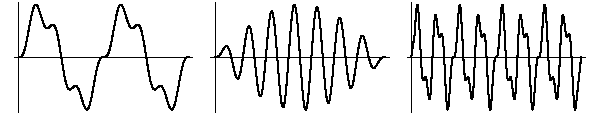
\includegraphics[width=\textwidth]{ode/inhomogeneous/non_res_forcing}
      \end{center}
      \caption{Non-resonant forcing.}
      \label{non_res_forcing}
    \end{figure}

    For $\lambda = 1$, we have
    \begin{align*}
      y       &= \frac{1}{2} \int_0^t \big( \cos(t - 2 \tau) - \cos(tau) \big) \,\dd \tau\\
      &= \frac{1}{2} \left[ - \frac{1}{2} \sin( t - 2 \tau) - \tau \cos t
      \right]_0^t
    \end{align*}
    \begin{equation}
      \label{res_forcing_soln}
      \boxed{
        y = \frac{1}{2} \left( \sin t - t \cos t \right).
        }
    \end{equation}
    The solution has both a periodic and a transient term.
    This solution is plotted in Figure~\ref{non_res_forcing}
    on the interval $t \in [0,16 \pi]$.
    \begin{figure}[tb!]
      \begin{center}
        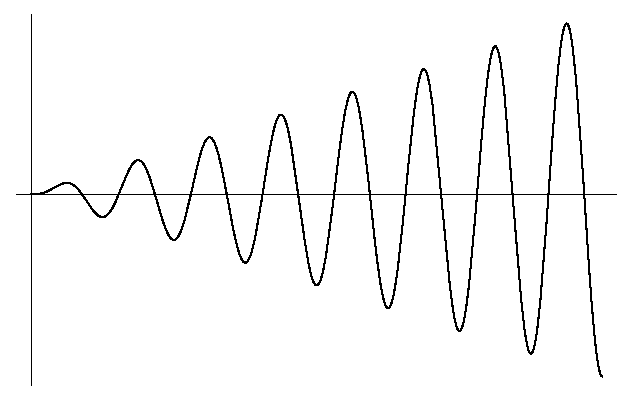
\includegraphics[width=0.3\textwidth]{ode/inhomogeneous/res_forcing}
      \end{center}
      \caption{Resonant forcing.}
      \label{res_forcing}
    \end{figure}

    Note that we can derive (\ref{res_forcing_soln}) from
    (\ref{non_res_forcing_soln}) by
    taking the limit as $\lambda \to 0$.
    \begin{align*}
      \lim_{\lambda \to 1} \frac{ \sin(\lambda t) - \lambda \sin t }{ 1 - \lambda^2 }
      &= \lim_{\lambda \to 1} \frac{ t \cos(\lambda t) - \sin t }
      {- 2 \lambda} \\
      &= \frac{1}{2} \left( \sin t - t \cos t \right)
    \end{align*}
  \end{enumerate}
\end{Solution}






%%222222222222222222222222222222222222222222222222222222222222222222222222222
\begin{Solution}
  \label{solution y+p2y+p1y+p0y=f}
  Let $y_1$, $y_2$ and $y_3$ be linearly independent homogeneous solutions
  to the differential equation
  \[ L[y] = y''' + p_2 y'' + p_1 y' + p_0 y = f(x). \]
  We will look for a particular solution of the form
  \[ y_p = u_1 y_1 + u_2 y_2 + u_3 y_3. \]
  Since the $u_j$'s are undetermined functions, we are free to impose two
  constraints.  We choose the constraints to simplify the algebra.
  \begin{align*}
    u_1' y_1 + u_2' y_2 + u_3' y_3 &= 0 \\
    u_1' y_1'+ u_2' y_2'+ u_3' y_3'&= 0
  \end{align*}
  Differentiating the expression for $y_p$,
  \begin{align*}
    y_p'    &= u_1' y_1 + u_1 y_1' + u_2' y_2 + u_2 y_2' + u_3' y_3 + u_3 y_3' \\
    &= u_1 y_1' + u_2 y_2' + u_3 y_3' \\
    y_p''   &= u_1' y_1' + u_1 y_1'' + u_2' y_2' + u_2 y_2'' 
    + u_3' y_3' + u_3 y_3'' \\
    &= u_1 y_1'' + u_2 y_2'' + u_3 y_3'' \\
    y_p'''  &= u_1' y_1'' + u_1 y_1''' + u_2' y_2'' + u_2 y_2''' 
    + u_3' y_3'' + u_3 y_3''' 
  \end{align*}
  Substituting the expressions for $y_p$ and its derivatives into the 
  differential equation,
  \begin{align*}
    &u_1' y_1'' + u_1 y_1''' + u_2' y_2'' + u_2 y_2''' + u_3' y_3'' + u_3 y_3'''
    + p_2 (u_1 y_1'' + u_2 y_2'' + u_3 y_3'')
    + p_1 (u_1 y_1' + u_2 y_2' + u_3 y_3') \\
    &\qquad + p_0 (u_1 y_1 + u_2 y_2 + u_3 y_3) = f(x) 
  \end{align*}
  \begin{gather*}
    u_1' y_1'' + u_2' y_2'' + u_3' y_3'' + u_1 L[y_1] + u_2 L[y_2] + u_3 L[y_3]
    = f(x) \\
    u_1' y_1'' + u_2' y_2'' + u_3' y_3'' = f(x).
  \end{gather*}
  With the two constraints, we have the system of equations,
  \begin{align*}
    u_1' y_1 + u_2' y_2 + u_3' y_3 &= 0 \\
    u_1' y_1'+ u_2' y_2'+ u_3' y_3'&= 0 \\
    u_1' y_1'' + u_2' y_2'' + u_3' y_3'' &= f(x)
  \end{align*}
  We solve for the $u_j'$ using Kramer's rule.
  \[ u_1' = \frac{(y_2 y_3' - y_2' y_3)f(x)}{W(x)}, \quad
  u_2' = -\frac{(y_1 y_3' - y_1' y_3)f(x)}{W(x)}, \quad
  u_3' = \frac{(y_1 y_2' - y_1' y_2)f(x)}{W(x)} \]
  Here $W(x)$ is the Wronskian of $\{y_1, y_2, y_3\}$.  Integrating the 
  expressions for $u_j'$, the particular solution is
  \[ \boxed{ y_p = y_1 \int \frac{(y_2 y_3' - y_2' y_3) f(x)}{W(x)}\,\dd x
    + y_2 \int \frac{(y_3 y_1' - y_3' y_1) f(x)}{W(x)}\,\dd x
    + y_3 \int \frac{(y_1 y_2' - y_1' y_2) f(x)}{W(x)}\,\dd x. }\]
\end{Solution}


%%-----------------------------------------------------------------------------
\begin{large}
  \noindent
  \textbf{Green Functions}
\end{large}



%% y'' = f(x), \quad y(-\infty) = y'(-\infty) = 0.
\begin{Solution}
  \label{solution y=f y=y=0}
  We consider the Green function problem
  \[
  G'' = f(x), \quad G(-\infty|\xi) = G'(-\infty|\xi) = 0.
  \]
  The homogeneous solution is $y = c_1 + c_2 x$.  The homogeneous solution
  that satisfies the boundary conditions is $y = 0$.  Thus the Green function
  has the form
  \[
  G(x|\xi) = 
  \begin{cases}
    0 &x < \xi, \\
    c_1 + c_2 x & x > \xi.
  \end{cases}
  \]
  The continuity and jump conditions are then
  \[
  G(\xi^+|\xi) = 0, \quad G'(\xi^+|\xi) = 1.
  \]
  Thus the Green function is
  \[
  G(x|\xi) = 
  \begin{cases}
    0 &x < \xi, \\
    x - \xi & x > \xi
  \end{cases}
  = (x - \xi) H(x - \xi).
  \]
  The solution of the problem 
  \[
  y'' = f(x), \quad y(-\infty) = y'(-\infty) = 0.
  \]
  is
  \begin{gather*}
    y = \int_{-\infty}^\infty f(\xi) G(x|\xi) \,\dd \xi \\
    y = \int_{-\infty}^\infty f(\xi) (x - \xi) H(x - \xi) \,\dd \xi \\
    \boxed{
      y = \int_{-\infty}^x f(\xi) (x - \xi) \,\dd \xi 
      }
  \end{gather*}
  We differentiate this solution to verify that it satisfies the differential
  equation.
  \begin{gather*}
    y' = \left[ f(\xi) (x - \xi) \right]_{\xi = x} 
    + \int_{-\infty}^x \frac{\partial}{\partial x} \left( f(\xi) (x - \xi) 
    \right) \,\dd \xi 
    = \int_{-\infty}^x f(\xi) \,\dd \xi \\
    y'' = \left[ f(\xi) \right]_{\xi = x} = f(x)
  \end{gather*}
\end{Solution}






%%111111111111111111111111111111111111111111111111111111111111111111111111111
\begin{Solution}
  \label{solution y+1xy-1x2y=x2}
  Since we are dealing with an Euler equation, we substitute $y = x^\lambda$
  to find the homogeneous solutions.
  \begin{gather*}
    \lambda(\lambda-1) + \lambda - 1 = 0 \\
    (\lambda-1)(\lambda+1) = 0 \\
    y_1 = x, \qquad y_2 = \frac{1}{x}
  \end{gather*}

  \paragraph{Variation of Parameters.}
  The Wronskian of the homogeneous solutions is
  \[W(x) = 
  \begin{vmatrix}
    x       & 1/x \\
    1       & -1/x^2
  \end{vmatrix}
  = -\frac{1}{x} - \frac{1}{x} = -\frac{2}{x}.
  \]
  A particular solution is
  \begin{align*}
    y_p     &= - x \int \frac{x^2(1/x)}{-2/x}\,\dd x 
    + \frac{1}{x} \int \frac{x^2 x}{-2/x}\,\dd x \\
    &= -x \int -\frac{x^2}{2}\,\dd x 
    + \frac{1}{x} \int -\frac{x^4}{2}\,\dd x \\
    &= \frac{x^4}{6} - \frac{x^4}{10} \\
    &= \frac{x^4}{15}.
  \end{align*}
  The general solution is
  \[y = \frac{x^4}{15} + c_1 x + c_2 \frac{1}{x}.\]
  Applying the initial conditions,
  \begin{alignat*}{2}
    y(0) &= 0 \quad &\to \quad c_2 &= 0 \\
    y'(0) &= 0 \quad &\to \quad c_1 &= 1.
  \end{alignat*}
  Thus we have the solution 
  \[ \boxed{y = \frac{x^4}{15} + x.} \]



  \paragraph{Green Function.}
  Since this problem has both an inhomogeneous term in the differential equation
  and inhomogeneous boundary conditions, we separate it into the two problems
  \begin{alignat*}{2}
    &u'' + \frac{1}{x} u' - \frac{1}{x^2} u = x^2, &\qquad &u(0) = u'(0) = 0, \\
    &v'' + \frac{1}{x} v' - \frac{1}{x^2} v = 0, &\qquad &v(0) = 0,\ v'(0) = 1.
  \end{alignat*}

  First we solve the inhomogeneous differential equation with the homogeneous
  boundary conditions.  The Green function for this problem satisfies
  \[ L[G(x|\xi)] = \delta(x-\xi), \quad G(0|\xi) = G'(0|\xi) = 0. \]
  Since the Green function must satisfy the
  homogeneous boundary conditions, it has the form
  \[ G(x|\xi) = 
  \begin{cases}
    0 \quad &\mathrm{for}\ x < \xi \\
    c x + d/x \quad &\mathrm{for}\ x > \xi.
  \end{cases}
  \]
  From the continuity condition,
  \[ 0 = c \xi + d / \xi.\]
  The jump condition yields
  \[ c - d/ \xi^2 = 1.\]
  Solving these two equations, we obtain
  \[ G(x|\xi) = 
  \begin{cases}
    0 \quad &\mathrm{for}\ x < \xi \\
    \frac{1}{2} x - \frac{\xi^2}{2 x} \quad &\mathrm{for}\ x > \xi
  \end{cases}
  \]
  Thus the solution is
  \begin{align*}
    u(x)    &= \int_0^\infty G(x|\xi) \xi^2\,\dd \xi \\
    &= \int_0^x \left(\frac{1}{2} x - \frac{\xi^2}{2 x}\right)\xi^2\,\dd \xi\\
    &= \frac{1}{6}x^4 - \frac{1}{10}x^4 \\
    &= \frac{x^4}{15}.
  \end{align*}

  Now to solve the homogeneous differential equation with inhomogeneous 
  boundary conditions.
  The general solution for $v$ is
  \[ v = c x + d / x. \]
  Applying the two boundary conditions gives
  \[ v = x.\]

  Thus the solution for $y$ is
  \[ \boxed{y = x + \frac{x^4}{15}.} \]
\end{Solution}












%%333333333333333333333333333333333333333333333333333333333333333333333333333333
\begin{Solution}
  \label{solution continuity y+p2y+p1y+p0y=f}
  The Green function satisfies
  \[
  G'''(x|\xi) + p_2(x) G''(x|\xi) + p_1(x) G'(x|\xi) + p_0(x) G(x|\xi) 
  = \delta(x-\xi).
  \]
  First note that only the $G'''(x|\xi)$ term can have a delta function 
  singularity.  If a lower derivative had a delta function type singularity, 
  then $G'''(x|\xi)$ would be more singular than a delta function and there
  would be no other term in the equation to balance that behavior.  Thus we see 
  that $G'''(x|\xi)$ will have a delta function singularity; $G''(x|\xi)$ will
  have a jump discontinuity; $G'(x|\xi)$ will be continuous at $x=\xi$.
  Integrating the differential equation from $\xi^-$ to $\xi^+$ yields
  \[
  \int_{\xi^-}^{\xi^+} G'''(x|\xi) \,\dd x
  = \int_{\xi^-}^{\xi^+} \delta(x-\xi) \,\dd x
  \]
  \[
  G''(\xi^+|\xi) - G''(\xi^-|\xi) = 1.
  \]
  Thus we have the three continuity conditions:
  \begin{align*}
    G''(\xi^+|\xi) &= G''(\xi^-|\xi) + 1 \\
    G'(\xi^+|\xi) &= G'(\xi^-|\xi) \\
    G(\xi^+|\xi) &= G(\xi^-|\xi) 
  \end{align*}
\end{Solution}















%%44444444444444444444444444444444444444444444444444444444444444444444444444444
\begin{Solution}
  \label{solution x2y-2xy+2y=e-x}
  \textbf{Variation of Parameters.}
  Consider the problem
  \[ 
  x^2 y'' - 2 x y' + 2 y = \e^{-x}, \qquad y(1) = 0, \quad y'(1) = 1. 
  \]
  Previously we showed that two homogeneous solutions are
  \[ 
  y_1 = x, \qquad y_2 = x^2. 
  \]
  The Wronskian of these solutions is
  \[ 
  W(x) =
  \begin{vmatrix}
    x       &       x^2     \\
    1       &       2x
  \end{vmatrix}
  = 2x^2 - x^2 = x^2.
  \]
  In the variation of parameters formula, we will choose $1$ as the lower
  bound of integration.  (This will simplify the algebra in applying the
  initial conditions.)
  \begin{align*}
    y_p     &= -x \int_1^x \frac{\e^{-\xi} \xi^2}{\xi^4}\,\dd \xi + x^2 \int_1^x
    \frac{\e^{-\xi} \xi}{\xi^4}\,\dd \xi \\
    &= -x \int_1^x \frac{\e^{-\xi}}{\xi^2} \,\dd \xi 
    + x^2 \int_1^x \frac{\e^{-\xi}}{\xi^3} \,\dd \xi \\
    &= -x \left(\e^{-1}-\frac{\e^{-x}}{x} 
      - \int_1^x \frac{\e^{-\xi}}{\xi} \,\dd \xi \right)
    + x^2 \left( \frac{\e^{-x}}{2x} - \frac{\e^{-x}}{2x^2}
      + \frac{1}{2}\int_1^x \frac{\e^{-\xi}}{\xi} \,\dd \xi \right)\\
    &= -x \e^{-1} + \frac{1}{2} (1+x) \e^{-x} 
    + \left(\frac{x+x^2}{2}\right) 
    \int_1^x \frac{\e^{-\xi}}{\xi} \,\dd \xi
  \end{align*}
  If you wanted to, you could write the last integral in terms of exponential
  integral functions.

  The general solution is
  \[ 
  y = c_1 x + c_2 x^2  -x \e^{-1} + \frac{1}{2} (1+x) \e^{-x} 
  + \left(x+\frac{x^2}{2}\right) \int_1^x \frac{\e^{-\xi}}{\xi} \,\dd \xi
  \]
  Applying the boundary conditions,
  \begin{alignat*}{3}
    &y(1) = 0 &\qquad &\to &\qquad &c_1 + c_2 = 0 \\
    &y'(1) = 1 &\qquad &\to &\qquad &c_1 + 2 c_2 = 1,
  \end{alignat*}
  we find that $c_1 = -1$, $c_2 = 1$.

  Thus the solution subject to the initial conditions is
  \[ 
  \boxed{ 
    y = -(1+\e^{-1})x + x^2 + \frac{1}{2} (1+x) \e^{-x} 
    + \left(x+\frac{x^2}{2}\right) \int_1^x \frac{\e^{-\xi}}{\xi} \,\dd \xi
    }
  \]

  \textbf{Green Functions.}
  The solution to the problem is $y=u+v$ where 
  \[
  u'' - \frac{2}{x} u' + \frac{2}{x^2} u = \frac{\e^{-x}}{x^2}, \qquad
  u(1)=0, \quad u'(1)=0,
  \]
  and
  \[
  v'' - \frac{2}{x} v' + \frac{2}{x^2} v = 0, \qquad v(1)=0, \quad v'(1)=1.
  \]
  The problem for $v$ has the solution
  \[
  v = -x + x^2.
  \]
  The Green function for $u$ is
  \[
  G(x|\xi) = H(x-\xi) u_\xi(x)
  \]
  where
  \[
  u_\xi(\xi) = 0, \quad \mathrm{and} \quad u_\xi'(\xi)=1.
  \]
  Thus the Green function is
  \[
  G(x|\xi) = H(x-\xi) \left(-x + \frac{x^2}{\xi} \right).
  \]
  The solution for $u$ is then
  \begin{align*}
    u       &= \int_1^\infty G(x|\xi) \frac{\e^{-\xi}}{\xi^2} \,\dd \xi \\
    &= \int_1^x \left(-x + \frac{x^2}{\xi} \right) 
    \frac{\e^{-\xi}}{\xi^2} \,\dd \xi \\
    &= -x \e^{-1} + \frac{1}{2}(1+x)\e^{-x} + \left(x+\frac{x^2}{2}\right)
    \int_1^x \frac{\e^{-\xi}}{\xi} \,\dd \xi.
  \end{align*}
  Thus we find the solution for $y$ is
  \[ 
  \boxed{ 
    y = -(1+\e^{-1})x + x^2 + \frac{1}{2} (1+x) \e^{-x} 
    + \left(x+\frac{x^2}{2}\right) \int_1^x \frac{\e^{-\xi}}{\xi} \,\dd \xi
    }
  \]
\end{Solution}





%% Find the Green function for \[ y'' - y = f(x), \qquad y'(0) = y(1) = 0. \]
\begin{Solution}
  \label{solution y-y=f y0=y1=0}
  The differential equation for the Green function is
  \[
  G'' - G = \delta(x - \xi), \qquad G_x(0|\xi) = G(1|\xi) = 0.
  \]
  Note that $\cosh(x)$ and $\sinh(x-1)$ are homogeneous solutions that satisfy
  the left and right boundary conditions, respectively.  The Wronskian of 
  these two solutions is
  \begin{align*}
    W(x)    &= \begin{vmatrix} \cosh(x) & \sinh(x-1) \\ \sinh(x) & \cosh(x-1)
    \end{vmatrix} \\
    &= \cosh(x) \cosh(x-1) - \sinh(x) \sinh(x-1) \\
    &= \frac{1}{4} \left( \left( \e^x + \e^{-x} \right)
      \left( \e^{x-1} + \e^{-x+1} \right) 
      - \left( \e^x - \e^{-x} \right)
      \left( \e^{x-1} - \e^{-x+1} \right) \right) \\
    &= \frac{1}{2} \left( \e^1 + \e^{-1} \right) \\
    &= \cosh(1).
  \end{align*}
  The Green function for the problem is then
  \[
  G(x|\xi) = \frac{ \cosh(x_<) \sinh(x_> - 1) }{ \cosh(1) },
  \]
  \[
  \boxed{
    G(x|\xi) = \begin{cases}
      \frac{ \cosh(x) \sinh(\xi-1) }{ \cosh(1) } &\mathrm{for}\ 0 \leq x \leq \xi, \\
      \frac{ \cosh(\xi) \sinh(x-1) }{ \cosh(1) } &\mathrm{for}\ \xi \leq x \leq 1. \\
    \end{cases}
    }
  \]
\end{Solution}





%% Find the Green function for \[ y'' - y = f(x), \qquad y(0) = y(\infty) = 0.\]
\begin{Solution}
  \label{solution y-y=f y0=yinf=0}
  The differential equation for the Green function is
  \[
  G'' - G = \delta(x - \xi), \qquad G(0|\xi) = G(\infty|\xi) = 0.
  \]
  Note that $\sinh(x)$ and $\e^{-x}$ are homogeneous solutions that satisfy
  the left and right boundary conditions, respectively.  The Wronskian of 
  these two solutions is
  \begin{align*}
    W(x)    &= \begin{vmatrix} \sinh(x) & \e^{-x} \\ \cosh(x) & - \e^{-x}
    \end{vmatrix} \\
    &= - \sinh(x) \e^{-x} - \cosh(x) \e^{-x} \\
    &= - \frac{1}{2} \left( \e^x - \e^{-x} \right) \e^{-x}
    - \frac{1}{2} \left( \e^x + \e^{-x} \right) \e^{-x} \\
    &= -1
  \end{align*}
  The Green function for the problem is then
  \[
  G(x|\xi) = - \sinh(x_<) \e^{-x_>}
  \]
  \[
  \boxed{
    G(x|\xi) = \begin{cases}
      - \sinh(x) \e^{-\xi} &\mathrm{for}\ 0 \leq x \leq \xi, \\
      - \sinh(\xi) \e^{-x} &\mathrm{for}\ \xi \leq x \leq \infty. \\
    \end{cases}
    }
  \]
\end{Solution}







%% Find the Green function for each of the following:
\begin{Solution}
  \label{solution xu+u=f}

  $\phantom{a}$  %% Force a line break

  \begin{itemize}
    %%
  \item[a)]
    The Green function problem is
    \[
    x G''(x|\xi) + G'(x|\xi) = \delta(x-\xi), \quad G(0|\xi)\ \mathrm{bounded,}\ 
    G(1|\xi) = 0.
    \]
    First we find the homogeneous solutions of the differential equation.
    \[
    x y'' + y' = 0
    \]
    This is an exact equation.
    \[
    \frac{\dd}{\dd x} [ x y' ] = 0
    \]
    \[
    y' = \frac{c_1}{x}
    \]
    \[
    y = c_1 \log x + c_2
    \]
    The homogeneous solutions $y_1 = 1$ and $y_2 = \log x$ satisfy the left and
    right boundary conditions, respectively.  The Wronskian of these solutions
    is
    \[
    W(x) = \begin{vmatrix} 1 & \log x \\ 0 & 1/x \end{vmatrix}
    = \frac{1}{x}.
    \]
    The Green function is
    \[
    G(x|\xi) = \frac{ 1 \cdot \log x_> }{ \xi (1/\xi) },
    \]
    \[
    \boxed{
      G(x|\xi) = \log x_>.
      }
    \]
    %%
  \item[b)]
    The Green function problem is
    \[
    G''(x|\xi) - G(x|\xi) = \delta(x-\xi), \quad
    G(-a|\xi) = G(a|\xi) = 0.
    \]
    $\{\e^x, \e^{-x}\}$ and $\{ \cosh x, \sinh x\}$ are both linearly independent
    sets of homogeneous solutions.  $\sinh(x+a)$ and $\sinh(x-a)$ are homogeneous
    solutions that satisfy the left and right boundary conditions, respectively.
    The Wronskian of these two solutions is,
    \begin{align*}
      W(x)    &= \begin{vmatrix} \sinh(x+a) & \sinh(x-a) \\
        \cosh(x+a) & \cosh(x-a) \end{vmatrix} \\
      &= \sinh(x+a) \cosh(x-a) - \sinh(x-a) \cosh(x+a)  \\
      &= \sinh(2 a)
    \end{align*}
    The Green function is
    \[
    \boxed{
      G(x|\xi) = \frac{ \sinh(x_< + a) \sinh(x_> - a) }{ \sinh(2 a) }.
      }
    \]
    %%
  \item[c)]
    The Green function problem is
    \[
    G''(x|\xi) - G(x|\xi) = \delta(x - \xi), \quad
    G(x|\xi)\ \mathrm{bounded as}\ |x| \to \infty.
    \]
    $\e^{x}$ and $\e^{-x}$ are homogeneous solutions that satisfy the left 
    and right boundary conditions, respectively.  The Wronskian of these solutions
    is
    \[
    W(x) = \begin{vmatrix} \e^x & \e^{-x} \\ \e^x & - \e^{-x} \end{vmatrix}
    = -2.
    \]
    The Green function is
    \[
    G(x|\xi) = \frac{ \e^{x_<} \e^{- x_>} }{ -2 },
    \]
    \[
    \boxed{
      G(x|\xi) = - \frac{1}{2} \e^{x_< - x_>}.
      }
    \]
    %%
  \item[d)]
    The Green function from part (b) is,
    \[
    G(x|\xi) = \frac{ \sinh(x_< + a) \sinh(x_> - a) }{ \sinh(2 a) }.
    \]
    We take the limit as $a \to \infty$.
    \begin{align*}
      \lim_{a \to \infty} \frac{ \sinh(x_< + a) \sinh(x_> - a) }{ \sinh(2 a) }
      &= \lim_{a \to \infty} \frac{ 
        \left( \e^{x_< + a} - \e^{-x_< - a} \right)
        \left( \e^{x_> - a} - \e^{-x_> + a} \right) }
      { 2 \left( \e^{2 a} - \e^{-2 a} \right) } \\
      &= \lim_{a \to \infty} \frac{ -\e^{x_< - x_>} + \e^{x_< + x_> - 2a} 
        + \e^{-x_< - x_> - 2 a} - \e^{-x_< + x_> - 4a } }
      { 2 - 2 \e^{-4 a} } \\
      &= - \frac{ \e^{x_< - x_>} }{ 2 }
    \end{align*}
    Thus we see that the solution from part (b) approaches the solution from 
    part (c) as $a \to \infty$.
  \end{itemize}
\end{Solution}











%% For what values of $\lambda$ does the problem 
\begin{Solution}
  \label{solution y+lambday=f}
  \begin{enumerate}
  \item
    The problem,
    \[
    y'' + \lambda y = f(x), \quad y(0) = y(\pi) = 0,
    \]
    has a Green function if and only if it has a unique solution.  This 
    inhomogeneous problem has a unique solution if and only if the homogeneous
    problem has only the trivial solution.

    First consider the case $\lambda = 0$.  We find the general solution of the 
    homogeneous differential equation.
    \[
    y = c_1 + c_2 x
    \]
    Only the trivial solution satisfies the boundary conditions.  The problem
    has a unique solution for $\lambda = 0$.

    Now consider non-zero $\lambda$.  We find the general solution of the 
    homogeneous differential equation.
    \[
    y = c_1 \cos \left( \sqrt{\lambda} x \right)
    + c_2 \sin \left( \sqrt{\lambda} x \right).
    \]
    The solution that satisfies the left boundary condition is
    \[
    y = c \sin \left( \sqrt{\lambda} x \right).
    \]
    We apply the right boundary condition and find nontrivial solutions.
    \begin{gather*}
      \sin \left( \sqrt{\lambda} \pi \right) = 0
      \\
      \lambda = n^2, \quad n \in \mathbb{Z}^+
    \end{gather*}
    Thus the problem has a unique solution for all complex $\lambda$ except
    $\lambda = n^2$, $n \in \mathbb{Z}^+$.

    Consider the case $\lambda = 0$.  We find solutions of the homogeneous equation 
    that satisfy the left and right boundary conditions, respectively.
    \[
    y_1 = x, \qquad y_2 = x - \pi.
    \]
    We compute the Wronskian of these functions.
    \[
    W(x) = 
    \begin{vmatrix}
      x & x - \pi \\
      1 & 1 
    \end{vmatrix}
    = \pi.
    \]
    The Green function for this case is
    \[
    G(x|\xi) = \frac{x_< (x_> - \pi)}{\pi}.
    \]
    We consider the case $\lambda \neq n^2$, $\lambda \neq 0$.  
    We find the solutions of the homogeneous equation that satisfy 
    the left and right boundary conditions, respectively.
    \[
    y_1 = \sin \left( \sqrt{\lambda} x \right), \qquad 
    y_2 = \sin \left( \sqrt{\lambda} (x - \pi) \right).
    \]
    We compute the Wronskian of these functions.
    \[
    W(x) = 
    \begin{vmatrix}
      \sin \left( \sqrt{\lambda} x \right) &
      \sin \left( \sqrt{\lambda} (x - \pi) \right) \\
      \sqrt{\lambda} \cos \left( \sqrt{\lambda} x \right) &
      \sqrt{\lambda} \cos \left( \sqrt{\lambda} (x - \pi) \right)
    \end{vmatrix}
    = \sqrt{\lambda} \sin \left( \sqrt{\lambda} \pi \right)
    \]
    The Green function for this case is
    \[
    G(x|\xi) = \frac{ \sin \left( \sqrt{\lambda} x_< \right)
      \sin \left( \sqrt{\lambda} (x_> - \pi ) \right) }
    { \sqrt{\lambda} \sin \left( \sqrt{\lambda} \pi \right) }.
    \]

  \item
    Now we consider the problem
    \[
    y'' + 9 y = 1 + \alpha x, \quad y(0) = y(\pi) = 0.
    \]
    The homogeneous solutions of the problem
    are constant multiples of $\sin(3 x)$.  
    Thus for each value of $\alpha$, the problem either has no solution or an
    infinite number of solutions.  There will be an infinite number
    of solutions if the inhomogeneity $1 + \alpha x$ is orthogonal to the
    homogeneous solution $\sin(3 x)$ and no solution otherwise.
    \[
    \int_0^\pi (1 + \alpha x) \sin(3 x) \,\dd x = \frac{\pi \alpha + 2}{3}
    \]
    The problem has a solution only for $\alpha = - 2/\pi$.  For this case 
    the general solution of the inhomogeneous differential equation is
    \[
    y = \frac{1}{9} \left( 1 - \frac{2 x}{\pi} \right) + c_1 \cos(3 x) 
    + c_2 \sin(3 x).
    \]
    The one-parameter family of solutions that satisfies the boundary 
    conditions is
    \[
    y = \frac{1}{9} \left( 1 - \frac{2 x}{\pi} - \cos(3 x) \right) + c \sin(3 x).
    \]

  \item
    For $\lambda = n^2$, $n \in \mathbb{Z}^+$, $y = \sin(n x)$ is a solution of the
    homogeneous equation that satisfies the boundary conditions.
    Equation~\ref{eqn y'' + lambda y = f, y = y = 0} has a (non-unique) 
    solution only if $f$ is orthogonal to $\sin(n x)$.
    \[
    \int_0^\pi f(x) \sin(n x) \,\dd x = 0
    \]
    The modified Green function satisfies
    \[
    G'' + n^2 G = \delta(x - \xi) - \frac{ \sin(n x) \sin(n \xi) }{ \pi / 2 }.
    \]
    We expand $G$ in a series of the eigenfunctions.
    \[
    G(x|\xi) = \sum_{k = 1}^\infty g_k \sin(k x)
    \]
    We substitute the expansion into the differential equation to determine the
    coefficients.  This will not determine $g_n$.  We choose $g_n = 0$, which is 
    one of the choices that will make the modified Green function symmetric in
    $x$ and $\xi$.
    \begin{gather*}
      \sum_{k = 1}^\infty g_k \left( n^2 - k^2 \right) \sin(k x) 
      = \frac{2}{\pi} \sum_{\substack{k = 1 \\ k \neq n}}^\infty \sin(k x) \sin(k \xi)
      \\
      \boxed{
        G(x|\xi) = \frac{2}{\pi} \sum_{\substack{k = 1 \\ k \neq n}}^\infty 
        \frac{ \sin(k x) \sin(k \xi) }{ n^2 - k^2 }
        }
    \end{gather*}
    The solution of the inhomogeneous problem is
    \[
    y(x) = \int_0^\pi f(\xi) G(x|\xi) \,\dd \xi.
    \]
  \end{enumerate}
\end{Solution}









%% Show that the inhomogeneous boundary value problem:
\begin{Solution}
  \label{solution Lu=pu+qu=f}
  We separate the problem for $u$ into the two problems:
  \begin{gather*}
    L v \equiv (p v')' + q v = f(x), \quad a < x < b, 
    \quad v(a) = 0, \quad v(b) = 0 \\
    L w \equiv (p w')' + q w = 0, \quad a < x < b, 
    \quad w(a) = \alpha, \quad w(b) = \beta 
  \end{gather*}
  and note that the solution for $u$ is $u = v + w$.  

  The problem for $v$ has the solution,
  \[
  v = \int_a^b g(x;\xi) f(\xi) \,\dd \xi,
  \]
  with the Green function,
  \[
  g(x;\xi) = \frac{v_1(x_<) v_2(x_>)}{ p(\xi) W(\xi) } \equiv
  \begin{cases}
    \frac{v_1(x) v_2(\xi)}{ p(\xi) W(\xi) } &\mathrm{for}\ a \leq x \leq \xi, \\
    \frac{v_1(\xi) v_2(x)}{ p(\xi) W(\xi) } &\mathrm{for}\ \xi \leq x \leq b. \\
  \end{cases}
  \]
  Here $v_1$ and $v_2$ are homogeneous solutions that respectively satisfy 
  the left and right homogeneous boundary conditions.

  Since $g(x;\xi)$ is a solution of the homogeneous equation for $x \neq \xi$,
  $g_\xi(x;\xi)$ is a solution of the homogeneous equation for $x \neq \xi$.
  This is because for $x \neq \xi$, 
  \[
  L \left[ \frac{\partial}{\partial \xi} g \right] = \frac{\partial}{\partial \xi} L[g]
  = \frac{\partial}{\partial \xi} \delta(x-\xi) = 0.
  \]
  If $\xi$ is outside of the domain, $(a,b)$, then $g(x;\xi)$ and
  $g_\xi(x;\xi)$ are homogeneous solutions on that domain.  In particular
  $g_\xi(x;a)$ and $g_\xi(x;b)$ are homogeneous solutions,
  \[
  L \left[ g_\xi(x;a) \right] = L \left[ g_\xi(x;b) \right] = 0.
  \]
  Now we use the definition of the Green function and $v_1(a) = v_2(b) = 0$
  to determine simple expressions for these homogeneous solutions.
  \begin{align*}
    g_\xi(x;a) &= \frac{ v_1'(a) v_2(x) }{ p(a) W(a) }
    - \frac{ (p'(a) W(a) + p(a) W'(a)) v_1(a) v_2(x) }{ (p(a) W(a))^2 } \\
    &= \frac{ v_1'(a) v_2(x) }{ p(a) W(a) } \\
    &= \frac{ v_1'(a) v_2(x) }{ p(a) (v_1(a) v_2'(a) - v_1'(a) v_2(a)) } \\
    &= - \frac{ v_1'(a) v_2(x) }{ p(a) v_1'(a) v_2(a) } \\
    &= - \frac{ v_2(x) }{ p(a) v_2(a) } 
  \end{align*}
  We note that this solution has the boundary values,
  \[
  g_\xi(a;a) = - \frac{ v_2(a) }{ p(a) v_2(a) } = - \frac{1}{p(a)}, \qquad
  g_\xi(b;a) = - \frac{ v_2(b) }{ p(a) v_2(a) } = 0.
  \]
  We examine the second solution.
  \begin{align*}
    g_\xi(x;b) &= \frac{ v_1(x) v_2'(b) }{ p(b) W(b) }
    - \frac{ (p'(b) W(b) + p(b) W'(b)) v_1(x) v_2(b) }{ (p(b) W(b))^2 } \\
    &= \frac{ v_1(x) v_2'(b) }{ p(b) W(b) } \\
    &= \frac{ v_1(x) v_2'(b) }{ p(b) (v_1(b) v_2'(b) - v_1'(b) v_2(b)) } \\
    &= \frac{ v_1(x) v_2'(b) }{ p(b) v_1(b) v_2'(b) } \\
    &= \frac{ v_1(x) }{ p(b) v_1(b) } 
  \end{align*}
  This solution has the boundary values,
  \[
  g_\xi(a;b) = \frac{ v_1(a) }{ p(b) v_1(b) } = 0, \qquad
  g_\xi(b;b) = \frac{ v_1(b) }{ p(b) v_1(b) } = \frac{1}{p(b)}.
  \]
  Thus we see that the solution of 
  \[
  L w = (p w')' + q w = 0, \quad a < x < b, 
  \quad w(a) = \alpha, \quad w(b) = \beta,
  \]
  is
  \[
  w = - \alpha p(a) g_\xi(x;a) + \beta p(b) g_\xi(x;b).
  \]
  Therefore the solution of the problem for $u$ is
  \[
  \boxed{
    u = \int_a^b g(x;\xi) f(\xi) \,\dd \xi 
    - \alpha p(a) g_\xi(x;a) + \beta p(b) g_\xi(x;b).
    }
  \]
\end{Solution}








%% Green function for reduced wave equation by image method.
\begin{Solution}
  \label{solution u-k2u=f}
  Figure~\ref{helmholtz1am1} shows a plot of $G(x;1)$ and $G(x;-1)$ for $k=1$.

  \begin{figure}[tb!]
    \begin{center}
      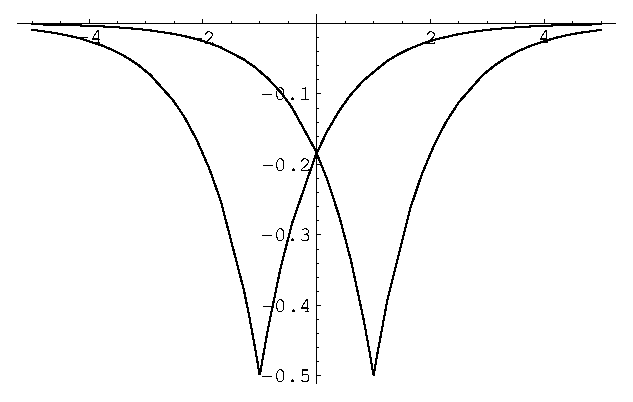
\includegraphics[width=0.4\textwidth]{ode/inhomogeneous/helmholtz1am1}
    \end{center}
    \caption{The Green functions.}
    \label{helmholtz1am1}
  \end{figure}

  First we consider the boundary condition $u(0) = 0$.  Note that the solution of
  \[
  G'' - k^2 G = \delta(x - \xi) - \delta(x+\xi), |G(\pm\infty;\xi)| < \infty,
  \]
  satisfies the condition $G(0;\xi) = 0$.  Thus the Green function which 
  satisfies $G(0;\xi) = 0$ is
  \[
  G(x;\xi) = - \frac{1}{2k} \e^{-k |x-\xi|} + \frac{1}{2k} \e^{-k |x+\xi|}.
  \]
  Since $x,\xi > 0$ we can write this as
  \begin{align*}
    G(x;\xi) &= - \frac{1}{2k} \e^{-k |x-\xi|} + \frac{1}{2k} \e^{-k (x+\xi)} \\
    &= \begin{cases}
      - \frac{1}{2k} \e^{-k (\xi-x)} + \frac{1}{2k} \e^{-k (x+\xi)},
      &\mathrm{for}\ x < \xi \\
      - \frac{1}{2k} \e^{-k (x-\xi)} + \frac{1}{2k} \e^{-k (x+\xi)},
      &\mathrm{for}\ \xi < x 
    \end{cases} \\
    &= \begin{cases}
      - \frac{1}{k} \e^{-k \xi} \sinh(k x), &\mathrm{for}\ x < \xi \\
      - \frac{1}{k} \e^{-k x} \sinh(k \xi), &\mathrm{for}\ \xi < x 
    \end{cases} \\
  \end{align*}
  \[
  \boxed{
    G(x;\xi) = - \frac{1}{k} \e^{-k x_>} \sinh(k x_<)
    }
  \]

  Now consider the boundary condition $u'(0) = 0$.  Note that the solution of
  \[
  G'' - k^2 G = \delta(x-\xi) + \delta(x+\xi), \quad |G(\pm\infty;\xi)| < \infty,
  \]
  satisfies the boundary condition $G'(x;\xi) = 0$.  Thus the Green function is
  \[
  G(x;\xi) = - \frac{1}{2k} \e^{-k |x-\xi|} - \frac{1}{2k} \e^{-k |x+\xi|}.
  \]
  Since $x,\xi > 0$ we can write this as
  \begin{align*}
    G(x;\xi) &= - \frac{1}{2k} \e^{-k |x-\xi|} - \frac{1}{2k} \e^{-k (x+\xi)} \\
    &= \begin{cases}
      - \frac{1}{2k} \e^{-k (\xi-x)} - \frac{1}{2k} \e^{-k (x+\xi)},
      &\mathrm{for}\ x < \xi \\
      - \frac{1}{2k} \e^{-k (x-\xi)} - \frac{1}{2k} \e^{-k (x+\xi)},
      &\mathrm{for}\ \xi < x 
    \end{cases} \\
    &= \begin{cases}
      - \frac{1}{k} \e^{-k \xi} \cosh(k x), &\mathrm{for}\ x < \xi \\
      - \frac{1}{k} \e^{-k x} \cosh(k \xi), &\mathrm{for}\ \xi < x 
    \end{cases} \\
  \end{align*}
  \[
  \boxed{
    G(x;\xi) = - \frac{1}{k} \e^{-k x_>} \cosh(k x_<)
    }
  \]

  The Green functions which satisfy $G(0;\xi) = 0$ and $G'(0;\xi) = 0$ 
  are shown in Figure~\ref{helmholtz1}.  We plot $G(x;1)$ and $G(x;-1)$.

  \begin{figure}[tb!]
    \begin{center}
      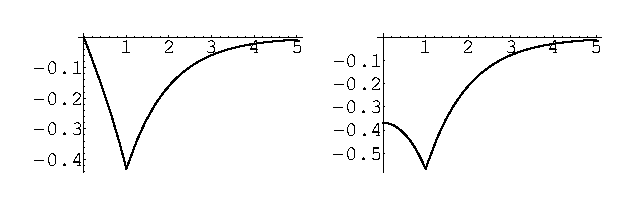
\includegraphics[width=0.5\textwidth]{ode/inhomogeneous/helmholtz1}
    \end{center}
    \caption{The Green functions.}
    \label{helmholtz1}
  \end{figure}
\end{Solution}






%% y'' - a^2 y = f(x), \quad y(0) = y'(L) = 0.
\begin{Solution}
  \label{solution y-a2y=f}
  \begin{enumerate}
    %%
    %%
  \item
    The Green function satisfies
    \[
    g'' - a^2 g = \delta(x - \xi), \quad g(0;\xi) = g'(L;\xi) = 0.
    \]
    We can write the set of homogeneous solutions as
    \[
    \left\{ \e^{a x}, \e^{-a x} \right\}\ \mathrm{or}\ 
    \left\{ \cosh(a x), \sinh(a x) \right\}.
    \]
    The solutions that respectively satisfy the left and right boundary conditions 
    are
    \[
    u_1 = \sinh(a x), \quad u_2 = \cosh(a (x - L)).
    \]
    The Wronskian of these solutions is
    \[
    W(x) = 
    \begin{pmatrix}
      \sinh(a x) & \cosh(a(x-L)) \\
      a \cosh(a x) & a \sinh(a(x-L))
    \end{pmatrix}
    = -a \cosh(a L).
    \]
    Thus the Green function is
    \[
    \boxed{
      g(x;\xi) = 
      \begin{cases}
        - \frac{ \sinh(a x) \cosh(a (\xi-L)) }{ a \cosh(a L) } 
        &\mathrm{for}\ x \leq \xi, \\
        - \frac{ \sinh(a \xi) \cosh(a (x-L)) }{ a \cosh(a L) } 
        &\mathrm{for}\ \xi \leq x. 
      \end{cases}
      =
      - \frac{ \sinh(a x_<) \cosh(a (x_> -L)) }{ a \cosh(a L) }.
      }
    \]
    %%
    %%
  \item
    We take the limit as $L \to \infty$.
    \begin{align*}
      g(x;\xi)
      &= \lim_{L \to \infty} - \frac{ \sinh(a x_<) \cosh(a (x_> -L)) }
      { a \cosh(a L) } \\
      &= \lim_{L \to \infty} - \frac{ \sinh(a x_<) }{ a }
      \frac{ \cosh( a x_> ) \cosh( a L ) 
        - \sinh( a x_> ) \sinh( a L ) }{ \cosh(a L) } \\
      &= - \frac{ \sinh(a x_<) }{ a }
      ( \cosh( a x_> ) - \sinh( a x_> ) ) 
    \end{align*}
    \[
    \boxed{
      g(x;\xi) = - \frac{1}{a} \sinh(a x_<) \e^{-a x_>} 
      }
    \]
    The solution of 
    \[
    y'' - a^2 y = \e^{-x}, \quad y(0) = y'(\infty) = 0
    \]
    is
    \begin{align*}
      y       &= \int_0^\infty g(x;\xi) \e^{-\xi} \,\dd \xi \\
      &= - \frac{1}{a} \int_0^\infty \sinh(a x_<) \e^{-a x_>} \e^{-\xi} \,\dd \xi \\
      &= - \frac{1}{a} \left( 
        \int_0^x \sinh(a \xi) \e^{-a x} \e^{- \xi} \,\dd \xi
        + \int_x^\infty \sinh(a x) \e^{-a \xi} \e^{-\xi} \,\dd \xi 
      \right) \\
      \intertext{We first consider the case that $a \neq 1$.}
      &= - \frac{1}{a} \left( 
        \frac{ \e^{-a x} }{a^2 - 1} \left( -a + \e^{-x} 
          ( a \cosh(a x) + \sinh(a x) ) \right)
        + \frac{1}{a+1} \e^{-(a+1) x} \sinh(a x)
      \right) \\
      &= \frac{ \e^{-a x} - \e^{-x} }{ a^2 - 1 }
    \end{align*}
    For $a = 1$, we have
    \begin{align*}
      y       &= - \left( \frac{1}{4} \e{-x} \left( -1 + 2 x + \e^{-2 x} \right)
        + \frac{1}{2} \e^{-2 x} \sinh(x) \right) \\
      &= - \frac{1}{2} x \e^{-x}.
    \end{align*}
    Thus the solution of the problem is
    \[
    \boxed{
      y = 
      \begin{cases}
        \frac{ \e^{-a x} - \e^{-x} }{ a^2 - 1 } &\mathrm{for}\ a \neq 1, \\
        - \frac{1}{2} x \e^{-x} &\mathrm{for}\ a = 1.
      \end{cases}
      }
    \]
    We note that this solution satisfies the differential equation and 
    the boundary conditions.
  \end{enumerate}
\end{Solution}







}



\raggedbottom
%%=============================================================================
\pagebreak
\flushbottom
\section{Quiz}


\begin{QuizProblem}
  \label{quiz problem y'' - y = f}
  Find the general solution of 
  \[
  y'' - y = f(x),
  \]
  where $f(x)$ is a known function.

  \quizsolution{y'' - y = f}
\end{QuizProblem}










\raggedbottom
%%=============================================================================
\pagebreak
\flushbottom
\section{Quiz Solutions}


\begin{QuizSolution}
  \label{quiz solution y'' - y = f}
  \[
  y'' - y = f(x)
  \]
  We substitute $y = \e^{\lambda x}$ into the homogeneous differential equation.
  \begin{gather*}
    y'' - y = 0 
    \\
    \lambda^2 \e^{\lambda x} - \e^{\lambda x} = 0 
    \\
    \lambda = \pm 1
  \end{gather*}
  The homogeneous solutions are $\e^{x}$ and $\e^{-x}$.  The Wronskian of 
  these solutions is
  \[
  \begin{vmatrix}
    \e^x & \e^{-x} 
    \\
    \e^x & - \e^{-x}
  \end{vmatrix}
  = - 2.
  \]
  We find a particular solution with variation of parameters.
  \[
  y_p = - \e^x \int \frac{\e^{-x} f(x)}{-2} \,\dd x
  + \e^{-x} \int \frac{\e^x f(x)}{-2} \,\dd x
  \]
  The general solution is
  \[
  y = c_1 \e^x + c_2 \e^{-x}
  - \e^x \int \frac{\e^{-x} f(x)}{-2} \,\dd x
  + \e^{-x} \int \frac{\e^x f(x)}{-2} \,\dd x.
  \]
\end{QuizSolution}







\raggedbottom


\flushbottom

%%%%
%% Improve the exposition of the section on Euler equations and add back in.
%%%%
%% Include all the material in chap 5 of Spiegel.
%%%%



%%===========================================================================
%%===========================================================================
\chapter{Difference Equations}

Televisions should have a dial to turn up the intelligence.  There is a 
brightness knob, but it doesn't work.

\begin{flushright}
  -?
\end{flushright}



%%============================================================================
\section{Introduction}
\begin{Example}
  \label{gambler's-ruin-intro}
  \index{gambler's ruin problem}
  \textbf{Gambler's ruin problem.}
  Consider a gambler that initially has $n$ dollars.  He plays a game in which
  he has a probability $p$ of winning a dollar and $q$ of losing a dollar.
  (Note that $p + q = 1$.)
  The gambler has decided that if he attains $N$ dollars he will stop playing
  the game.  In this case we will say that he has succeeded.  Of course if he 
  runs out of money before that happens, we will say that he is ruined.  What is
  the probability of the gambler's ruin?  Let us denote this probability by
  $a_n$.  We know that if he has no money left, then his ruin is certain, so 
  $a_0$ = 1.  If he reaches $N$ dollars he will quit the game, so that
  $a_N = 0$.  If he is somewhere in between ruin and success then the probability
  of his ruin is equal to $p$ times the probability of his ruin if he had
  $n+1$ dollars plus $q$ times the probability of his ruin if he had
  $n-1$ dollars.  Writing this in an equation,
  \[ a_n = pa_{n+1} + q a_{n-1} \quad \mathrm{subject to}\quad a_0=1, \quad
  a_N = 0.\]
  This is an example of a difference equation.  You will learn how to solve this
  particular problem in the section on constant coefficient equations.
\end{Example}




\index{discrete derivative}
Consider the sequence $a_1, a_2, a_3, \ldots$ Analogous to a derivative of
a continuous function, we can define a discrete derivative on the sequence
\[      D a_n = a_{n+1} - a_n. \]
The second discrete derivative is then defined as
\[      D^2a_n = D[a_{n+1} - a_n] = a_{n+2} - 2 a_{n+1} + a_n. \]
\index{discrete integral}
The discrete integral of $a_n$ is
\[      \sum_{i=n_0}^n a_i. \]
Corresponding to
\[ \int_\alpha^\beta \frac{\dd f}{\dd x}\,dx = f(\beta) - f(\alpha),\]
in the discrete realm we have
\[ \sum_{n=\alpha}^{\beta-1} D[a_n] = \sum_{n=\alpha}^{\beta-1} (a_{n+1}-a_n)
= a_\beta - a_\alpha. \]

Linear difference equations have the form 
\[ D^r a_n + p_{r-1}(n) D^{r-1}a_n + \cdots + p_1(n)D a_n + p_0(n)a_n = f(n).\]
From the definition of the discrete derivative an equivalent form is
\[ a_{n+r} + q_{r-1}(n) a_{n_r-1} + \cdots + q_1(n)a_{n+1} + q_0(n)a_n=f(n).\]

Besides being important in their own right, we will need to solve
difference equations in order to develop series solutions of 
differential equations.  Also, some methods of solving differential equations
numerically are based on approximating them with difference equations.

There are many similarities between differential and difference equations.
Like differential equations, an $r^{t h}$ order homogeneous difference 
equation has $r$ linearly independent solutions.  The general solution
to the $r^{t h}$ order inhomogeneous equation is the sum of the 
particular solution and an arbitrary linear combination of the homogeneous
solutions.  

For an $r^{t h}$ order difference equation, the initial condition is given
by specifying the values of the first $r$ $a_n$'s.



\begin{Example}
  Consider the difference equation $a_{n-2} - a_{n-1} - a_n = 0$ subject to
  the initial condition $a_1 = a_2 = 1$.  Note that although we may not 
  know a closed-form formula for the $a_n$ we can calculate the $a_n$ in 
  order by substituting into the difference equation.  The first few $a_n$ are
  $1, 1, 2, 3, 5, 8, 13, 21, \ldots$  We recognize this as the 
  Fibonacci sequence.  
\end{Example}





%%===========================================================================
\section{Exact Equations}
\index{difference equations!exact equations}
Consider the sequence $a_1, a_2, \ldots$.
Exact difference equations on this sequence have the form
\[ D[F(a_n, a_{n+1}, \ldots, n)] = g(n).\]
We can reduce the order of, (or solve for first order), 
this equation by summing from $1$ to $n-1$.
\begin{gather*}
  \sum_{j=1}^{n-1} D[F(a_j, a_{j+1}, \ldots, j)] = \sum_{j=1}^{n-1} g(j) \\
  F(a_n, a_{n+1}, \ldots, n) - F(a_1, a_2, \ldots, 1) = \sum_{j=1}^{n-1} g(j) \\
  F(a_n, a_{n+1}, \ldots, n) = \sum_{j=1}^{n-1} g(j) + F(a_1, a_2, \ldots, 1) 
\end{gather*}


\begin{Result}
  We can reduce the order of the exact difference equation
  \[ D[F(a_n, a_{n+1}, \ldots, n)] = g(n), \qquad \mathrm{for}\ n \geq 1\]
  by summing both sides of the equation to obtain
  \[F(a_n, a_{n+1}, \ldots, n) = \sum_{j=1}^{n-1} g(j) +F(a_1, a_2, \ldots, 1).\]
\end{Result}



\begin{Example} 
  Consider the difference equation, $D[n a_n] = 1$.   
  Summing both sides of this equation
  \begin{gather*} 
    \sum_{j=1}^{n-1} D[j a_j] = \sum_{j=1}^{n-1} 1 \\ 
    n a_n - a_1 = n-1 \\ 
    \boxed{ a_n = \frac{n + a_1 - 1}{n}.} 
  \end{gather*} 
\end{Example} 





%%============================================================================ 
\section{Homogeneous First Order} 
\index{difference equations!first order homogeneous} 
Consider the homogeneous first order difference equation
\[      a_{n+1} = p(n)a_n, \qquad \mathrm{for}\ n \geq 1. \] 
We can directly solve for $a_n$. 
\begin{align*} 
  a_n     &=     a_n \frac{a_{n-1}}{a_{n-1}} \frac{a_{n-2}}{a_{n-2}} \cdots  
  \frac{a_1}{a_1} \\ 
  &=     a_1 \frac{a_n}{a_{n-1}} \frac{a_{n-1}}{a_{n-2}} \cdots 
  \frac{a_2}{a_1}  \\ 
  &=     a_1 p(n-1)p(n-2) \cdots p(1) \\ 
  &=     a_1 \prod_{j=1}^{n-1} p(j) 
\end{align*} 


Alternatively, we could solve this equation by making it exact. 
Analogous to an integrating factor for differential equations,  
we multiply the equation by the summing factor
\[S(n) = \left[\prod_{j=1}^{n} p(j) \right]^{-1}. \] 
\begin{gather*} 
  a_{n+1} - p(n) a_n = 0 \\ 
  \frac{a_{n+1}}{\prod_{j=1}^{n} p(j)} - \frac{a_n}{\prod_{j=1}^{n-1} p(j)}=0\\ 
  D \left[\frac{a_n}{\prod_{j=1}^{n-1} p(j)} \right] = 0 \\ 
  \intertext{Now we sum from $1$ to $n-1$.} 
  \frac{a_n}{\prod_{j=1}^{n-1} p(j)} - a_1 = 0 \\ 
  a_n = a_1 \prod_{j=1}^{n-1} p(j) 
\end{gather*} 




\begin{Result} 
  The solution of the homogeneous first order difference equation
  \[ a_{n+1} = p(n)a_n, \qquad \mathrm{for}\ n \geq 1, \] 
  is  
  \[a_n = a_1 \prod_{j=1}^{n-1} p(j). \] 
\end{Result} 



\begin{Example} 
  Consider the equation $a_{n+1} = n a_n$ with the initial condition
  $a_1 = 1$. 
  \[      a_n = a_1 \prod_{j=1}^{n-1} j = (1) (n-1)!  
  = \Gamma(n) \] 
  Recall that $\Gamma(z)$ is the generalization of the factorial function.  For 
  positive integral values of the argument, $\Gamma(n) = (n-1)!$. 
\end{Example} 


%%============================================================================ 
\section{Inhomogeneous First Order}
\index{difference equations!first order inhomogeneous}
Consider the equation
\[a_{n+1} = p(n) a_n + q(n) \quad \mathrm{for} \quad n \geq 1. \]
Multiplying by $S(n)= \left[ \prod_{j=1}^{n} p(j) \right]^{-1}$ yields
\[ \frac{a_{n+1}}{\prod_{j=1}^{n} p(j)} - \frac{a_n}{\prod_{j=1}^{n-1} p(j)}
= \frac{q(n)}{\prod_{j=1}^{n} p(j)}.  \]
The left hand side is a discrete derivative.
\[ D \left[ \frac{a_n}{\prod_{j=1}^{n-1} p(j)} \right] = 
\frac{q(n)}{\prod_{j=1}^{n} p(j)} \]
Summing both sides from $1$ to $n-1$, 
\[ \frac{a_n}{\prod_{j=1}^{n-1} p(j)} - a_1 = 
\sum_{k=1}^{n-1} \left[ \frac{q(k)}{\prod_{j=1}^{k} p(j)} \right] \]
\[ a_n = \left[ \prod_{m=1}^{n-1} p(m) \right]
\left[ \sum_{k=1}^{n-1} \left[ \frac{q(k)}{\prod_{j=1}^{k} p(j)} 
  \right] + a_1  \right].   \]


\begin{Result}
  The solution of the inhomogeneous first order difference equation
  \[a_{n+1} = p(n) a_n + q(n) \quad \mathrm{for} \quad n \geq 1 \]
  is 
  \[ a_n = \left[ \prod_{m=1}^{n-1} p(m) \right]
  \left[ \sum_{k=1}^{n-1} \left[ \frac{q(k)}{\prod_{j=1}^{k} p(j)} 
    \right] + a_1  \right].   \]
\end{Result}








\begin{Example} 
  Consider the equation $a_{n+1} = n a_n + 1$ for $n \geq 1$.
  The summing factor is
  \begin{gather*}
    S(n) = \left[ \prod_{j=1}^n j \right]^{-1} = \frac{1}{n!}. \\
    \intertext{Multiplying the difference equation by the summing factor,}
    \frac{a_{n+1}}{n!} - \frac{a_n}{(n-1)!} = \frac{1}{n!} \\
    D\left[ \frac{a_n}{(n-1)!} \right] = \frac{1}{n!} \\
    \frac{a_n}{(n-1)!} - a_1 = \sum_{k=1}^{n-1} \frac{1}{k!} \\
    \boxed{ a_n = (n-1)! \left[ \sum_{k=1}^{n-1} \frac{1}{k!} 
        + a_1 \right].} 
  \end{gather*}
\end{Example}





\begin{Example}
  Consider the equation
  \[
  a_{n+1} = \lambda a_n + \mu, \quad \mathrm{for}\ n \geq 0.
  \]
  From the above result, (with the products and sums starting at zero instead
  of one), the solution is
  \begin{align*}
    a_0     &= \left[ \prod_{m=0}^{n-1} \lambda \right] 
    \left[ \sum_{k=0}^{n-1} \left[ \frac{\mu}
        {\prod_{j=0}^k \lambda} \right] + a_0 \right] \\
    &= \lambda^n \left[ \sum_{k=0}^{n-1} \left[ \frac{\mu}
        {\lambda^{k+1}} \right] + a_0 \right] \\
    &= \lambda^n \left[ \mu \frac{\lambda^{-n-1}-\lambda^{-1}}
      {\lambda^{-1} - 1} + a_0 \right] \\
    &= \lambda^n \left[ \mu \frac{\lambda^{-n}-1}
      {1 - \lambda} + a_0 \right] \\
    &= \mu \frac{1 - \lambda^n} {1 - \lambda} + a_0 \lambda^n. 
  \end{align*}
\end{Example}







%%============================================================================
\section{Homogeneous Constant Coefficient Equations}
\index{difference equations!constant coefficient equations}
Homogeneous constant coefficient equations have the form
\[ a_{n+N} + p_{N-1} a_{n+N-1} + \cdots + p_1 a_{n+1} + p_0 a_n = 0. \]
The substitution $a_n = r^n$ yields
\begin{align*}
  r^N + p_{N-1}r^{N-1} + \cdots + p_1 r + p_0 &= 0 \\
  (r-r_1)^{m_1}\cdots (r-r_k)^{m_k} &= 0.
\end{align*}

If $r_1$ is a distinct root then the associated linearly independent solution
is $r_1^n$.  If $r_1$ is a root of multiplicity $m > 1$ then the associated
solutions are $r_1^n, n r_1^n, n^2r_1^n, \ldots, n^{m-1} r_1^n$.



\begin{Result}
  Consider the homogeneous constant coefficient difference equation
  \[ a_{n+N} + p_{N-1} a_{n+N-1} + \cdots + p_1 a_{n+1} + p_0 a_n = 0. \]
  The substitution $a_n = r^n$ yields the equation
  \[(r-r_1)^{m_1}\cdots (r-r_k)^{m_k} = 0. \]
  A set of linearly independent solutions is
  \[ \{r_1^n, n r_1^n, \ldots, n^{m_1-1}r_1^n, \ldots, r_k^n, n r_k^n, \ldots,
  n^{m_k-1}r_k^n\}.\]
\end{Result}



\begin{Example}
  Consider the equation $a_{n+2} - 3a_{n+1} + 2a_n = 0$ with the initial 
  conditions $a_1 = 1$ and $a_2 = 3$.  The substitution $a_n = r^n$ yields
  \[      r^2 - 3r + 2 = (r-1)(r-2) = 0. \]
  Thus the general solution is
  \[      a_n = c_1 1^n + c_2 2^n. \]
  The initial conditions give the two equations,
  \begin{align*}
    a_1 = 1 &= c_1 + 2c_2  \\
    a_2 = 3 &= c_1 + 4c_2
  \end{align*}
  Since $c_1 = -1$ and $c_2 = 1$, the solution to the difference equation
  subject to the initial conditions is
  \[ a_n = 2^n - 1.\]
\end{Example}



\begin{Example}
  \index{gambler's ruin problem}
  Consider the gambler's ruin problem that was introduced in 
  Example~\ref{gambler's-ruin-intro}.
  The equation for the probability of the gambler's ruin at $n$ dollars is
  \[ a_n = pa_{n+1} + q a_{n-1} \quad \mathrm{subject to}\quad a_0=1, \quad
  a_N = 0.\]
  We assume that $0<p<1$.  
  With the substitution $a_n = r^n$ we obtain
  \[ r = p r^2 + q. \]
  The roots of this equation are
  \begin{align*}
    r       &= \frac{1 \pm \sqrt{1 - 4p q}}{2p} \\
    &= \frac{1 \pm \sqrt{1 - 4p(1-p)}}{2p} \\
    &= \frac{1 \pm \sqrt{(1 - 2p)^2}}{2p} \\
    &= \frac{1 \pm |1-2p|}{2p}.
  \end{align*}
  We will consider the two cases $p \neq 1/2$ and $p = 1/2$.
  \begin{description}
  \item{$\mathbf{p \boldsymbol{\neq} 1 \boldsymbol{/} 2}$\textbf{.}} 
    If $p < 1/2$, the roots are 
    \begin{gather*}
      r = \frac{1 \pm (1-2p)}{2p} \\
      r_1 = \frac{1-p}{p} = \frac{q}{p}, \qquad r_2 = 1.
    \end{gather*}
    If $p > 1/2$ the roots are
    \begin{gather*}
      r = \frac{1 \pm (2p-1)}{2p} \\
      r_1 = 1, \qquad r_2 = \frac{-p + 1}{p} = \frac{q}{p}.
    \end{gather*}
    Thus the general solution for $p \neq 1/2$ is
    \[a_n = c_1  + c_2\left(\frac{q}{p}\right)^n.\]
    The boundary condition $a_0=1$ requires that $c_1 + c_2 = 1$.  From the 
    boundary condition $a_N=0$ we have
    \begin{gather*}
      (1-c_2) + c_2 \left(\frac{q}{p}\right)^N = 0 \\
      c_2 = \frac{-1}{-1 + (q/p)^N} \\
      c_2 = \frac{p^N}{p^N-q^N}.
    \end{gather*}
    Solving for $c_1$,
    \begin{gather*}
      c_1 = 1 - \frac{p^N}{p^N-q^N} \\
      c_1 = \frac{-q^N}{p^N - q^N}.
    \end{gather*}
    Thus we have 
    \[\boxed{a_n =  \frac{-q^N}{p^N-q^N} 
      + \frac{p^N}{p^N-q^N}\left(\frac{q}{p}\right)^n.} \]

  \item{$\mathbf{p \boldsymbol{=} 1 \boldsymbol{/} 2}$\textbf{.}}
    In this case, the two roots of the polynomial are both $1$.  The 
    general solution is
    \[ a_n = c_1 + c_2 n.\]
    The left boundary condition demands that $c_1 = 1$.  From the right 
    boundary condition we obtain
    \begin{gather*}
      1 + c_2 N = 0 \\
      c_2 = -\frac{1}{N}.
    \end{gather*}
    Thus the solution for this case is
    \[ \boxed{a_n = 1 - \frac{n}{N}.} \]
    As a check that this formula makes sense, 
    we see that for $n = N/2$ the probability of ruin is 
    $1 - \frac{N/2}{N} = \frac{1}{2}$.
  \end{description}
\end{Example}





%%============================================================================
\section{Reduction of Order}
\index{reduction of order!difference equations}
Consider the difference equation
\begin{equation} \label{difference_a_n}
  (n+1)(n+2)a_{n+2}-3(n+1)a_{n+1}+2a_n = 0\quad \mathrm{for}\quad n \geq 0 
\end{equation}
We see that one solution to this equation is $a_n = 1/n!$.
Analogous to the reduction of order for differential equations, the substitution
$a_n = b_n / n!$ will reduce the order of the difference equation.
\begin{gather}
  \frac{(n+1)(n+2)b_{n+2}}{(n+2)!} - \frac{3(n+1)b_{n+1}}{(n+1)!} 
  + \frac{2b_n}{n!} = 0 \nonumber \\
  b_{n+2} - 3b_{n+1} + 2b_n = 0 \label{difference_b_n}
\end{gather}
At first glance it appears that we have not reduced the order of the equation,
but writing it in terms of discrete derivatives
\[D^2 b_n - D b_n = 0 \]
shows that we now have a first order difference equation for $D b_n$.
The substitution $b_n = r^n$ in equation~\ref{difference_b_n} yields the
algebraic equation
\[r^2 - 3r + 2 = (r-1)(r-2) = 0.\]
Thus the solutions are $b_n = 1$ and $b_n = 2^n$.  Only the $b_n=2^n$ 
solution will give us another linearly independent solution for $a_n$. 
Thus the second solution for $a_n$ is $a_n = b_n / n! = 2^n / n!$.
The general solution to equation~\ref{difference_a_n} is then
\[\boxed{ a_n = c_1 \frac{1}{n!} + c_2 \frac{2^n}{n!}. } \]


\begin{Result} 
  Let $a_n = s_n$ be a homogeneous solution of a linear difference equation. 
  The substitution $a_n = s_n b_n$ will yield a difference equation for $b_n$ 
  that is of order one less than the equation for $a_n$. 
\end{Result} 



%%=========================================================================== 
%%%%%%%%%%%%%%%%%%%%%%%%%%%%%%%%%%%%%%%%%%%%%%%%%%%%%%%%%%%%%%%%%%%%%%%%%%%%%%%%%%
%%\section{*Euler Equations} 
%%\index{difference equations!Euler equation} 
%%The second order homogeneous Euler difference equation has the form
%%\[ (n+1)n D^2 a_n + p_1 n D a_n + p_0 a_n = 0.\] 
%%We look for solutions of the form 
%%\[a_n = \frac{\Gamma(n+r)}{\Gamma(n)}.\] 
%%Recall that $\Gamma(x+1) = x \Gamma(x)$, and for non-negative integral $n$,  
%%$\Gamma(n+1) = n!$. 
%%Now we 
%%find the finite derivatives of $a_n = \Gamma(n+r)/\Gamma(n)$. 
%%\begin{align*} 
%%D a_n   &= D \frac{\Gamma(n+r)}{\Gamma(n)} \\ 
%%       &= \frac{\Gamma(n+1+r)}{\Gamma(n+1)} -  
%%               \frac{\Gamma(n+r)}{\Gamma(n)} \\ 
%%       &= \frac{(n+r)\Gamma(n+r)}{n\Gamma(n)} -  
%%               \frac{n\Gamma(n+r)}{n\Gamma(n)} \\ 
%%       &= \frac{r\Gamma(n+r)}{n\Gamma(n)} \\ 
%%D^2a_n  &= \frac{r\Gamma(n+1+r)}{(n+1)\Gamma(n+1)} -  
%%               \frac{r\Gamma(n+r)}{n\Gamma(n)} \\ 
%%       &= \frac{r(n+r)\Gamma(n+r)}{(n+1)n\Gamma(n)} -  
%%               \frac{r(n+1)\Gamma(n+r)}{(n+1)n\Gamma(n)} \\ 
%%       &= \frac{r(r-1)\Gamma(n+r)}{(n+1)n\Gamma(n)} 
%%\end{align*} 
%%Substituting these formulas into the difference equation, 
%%\begin{gather*} 
%%(n+1)n \frac{r(r-1)\Gamma(n+r)}{(n+1)n\Gamma(n)} +  
%%       p_1 n \frac{r\Gamma(n+r)}{n\Gamma(n)} +  
%%       p_0 \frac{\Gamma(n+r)}{\Gamma(n)} = 0 \\ 
%%r(r-1) + p_1 r + p_0 = 0. \\ 
%%\intertext{Factoring this equation,} 
%%(r-r_1)(r-r_2) = 0. 
%%\end{gather*} 
%%If the roots are distinct, then the general solution to the difference  
%%equation is 
%%\[ a_n = c_1 \frac{\Gamma(n+r_1)}{\Gamma(n)} +  
%%               c_2 \frac{\Gamma(n+r_2)}{\Gamma(n)}. \] 
%%If the roots are not distinct, then we can use reduction of order to find 
%%the second linearly independent solution. 

%%For the $n^{t h}$ order Euler equation we use the same approach as for  
%%the second order equation. 






%%\begin{Result} 
%%Consider the second order Euler difference equation
%%\[ (n+1)n D^2 a_n + p_1 n D a_n + p_0 a_n = 0.\] 
%%The substitution
%%\[a_n = \frac{\Gamma(n+r)}{\Gamma(n)}\] 
%%will yield the algebraic equation
%%\[(r-r_1)(r-r_2) = 0.\] 
%%If the roots are distinct, the linearly independent solutions are 
%%\[ a_n = \frac{\Gamma(n+r_1)}{\Gamma(n)} \qquad \mathrm{and} \qquad 
%%       a_n = \frac{\Gamma(n+r_2)}{\Gamma(n)}.\] 
%%If the roots are not distinct, reduction of order can be used to find the 
%%second solution. 
%%\end{Result} 







%%\begin{Example} 
%%Consider the difference equation
%%\[(n^2 + n)a_{n+2} - (2n^2 + 4n)a_{n+1} + (n^2+3n+2)a_n = 0.\] 
%%First we write this equation in terms of finite derivatives. 
%%\begin{gather*} 
%%(n^2 + n)(a_{n+2}-2a_{n+1}+a_n) + (-2n^2 -4n + 2n^2 + 2n)a_{n+1} 
%%       + (n^2 + 3n + 2 - n^2 - n)a_n = 0 \\ 
%%(n+1)n D^2a_n -2n a_{n+1} + (2n+2) a_n = 0 \\ 
%%(n+1)n D^2a_n -2n (a_{n+1} - a_n) + (2n + 2 - 2n)a_n = 0 \\ 
%%(n+1)n D^2a_n -2n D_n + 2 a_n = 0  
%%\end{gather*} 
%%We see that this is a second order Euler equation.  The substitution 
%%$a_n = \Gamma(n+r)/\Gamma(n)$ yields the algebraic equation 
%%\[r(r-1) - 2r + 2 = 0, \] 
%%which has roots $r_1 = 1$, $r_2 = 2$.  Thus the general solution is 
%%\begin{gather*} 
%%a_n = c_1 \frac{\Gamma(n+1)}{\Gamma(n)} + c_2 %%\frac{\Gamma(n+2)}{\Gamma(n)}\\ 
%%\boxed{a_n = c_1 n + c_2 (n+1)n.} 
%%\end{gather*} 
%%\end{Example} 





\raggedbottom
%%=========================================================================== 
\exercises{
\pagebreak
\flushbottom
\section{Exercises} 






\begin{Exercise}
  \label{exercise fibonacci}
  Find a formula for the $n^{t h}$ term in the Fibonacci sequence
  $1,1,2,3,5,8,13,\ldots$. 
  \index{Fibonacci sequence} 

  \hintsolution{fibonacci}
\end{Exercise} 




\begin{Exercise} 
  \label{exercise an2=2nan}
  Solve the difference equation
  \[ 
  a_{n+2} = \frac{2}{n} a_n, \quad a_1 = a_2 = 1. 
  \] 

  \hintsolution{an2=2nan}
\end{Exercise} 









\raggedbottom 
}
%%=========================================================================== 
\hints{
\pagebreak
\flushbottom
\section{Hints} 







\begin{Hint}
  \label{hint fibonacci}
  The difference equation corresponding to the Fibonacci sequence is 
  \[a_{n+2} - a_{n+1} - a_n = 0, \qquad a_1 = a_2 = 1. \] 
\end{Hint} 






\begin{Hint} 
  \label{hint an2=2nan}
  Consider this exercise as two first order difference equations; one for  
  the even terms, one for the odd terms. 
\end{Hint} 








\raggedbottom 
}
%%=========================================================================== 
\solutions{
\pagebreak
\flushbottom
\section{Solutions} 








\begin{Solution} 
  \label{solution fibonacci}
  We can describe the Fibonacci sequence with the difference equation 
  \begin{gather*} 
    a_{n+2} - a_{n+1} - a_n = 0, \qquad a_1 = a_2 = 1. \\ 
    \intertext{With the substitution $a_n = r^n$ we obtain the equation} 
    r^2 - r - 1 = 0. \\ 
    \intertext{This equation has the two distinct roots} 
    r_1 = \frac{1 + \sqrt{5}}{2}, \qquad r_2 = \frac{1 - \sqrt{5}}{2}. \\ 
    \intertext{Thus the general solution is} 
    a_n = c_1 \left(\frac{1 + \sqrt{5}}{2}\right)^n +  
    c_2 \left(\frac{1 - \sqrt{5}}{2}\right)^n. 
  \end{gather*} 
  From the initial conditions we have 
  \begin{alignat*}{2} 
    &c_1 r_1 +      &c_2 r_2        &= 1 \\ 
    &c_1 r_1^2 +    &c_2 r_2^2      &= 1. 
  \end{alignat*} 
  Solving for $c_2$ in the first equation, 
  \[c_2 = \frac{1}{r_2}(1 - c_1 r_1).\] 
  We substitute this into the second equation. 
  \begin{gather*} 
    c_1r_1^2 + \frac{1}{r_2}(1 - c_1 r_1)r_2^2 = 1 \\ 
    c_1(r_1^2 - r_1r_2) = 1-r_2 
  \end{gather*} 
  \begin{align*} 
    c_1     &= \frac{1-r_2}{r_1^2 - r_1r_2} \\ 
    &= \frac{1 - \frac{1-\sqrt{5}}{2}} 
    {\frac{1+\sqrt{5}}{2} \sqrt{5}} \\ 
    &= \frac{\frac{1+\sqrt{5}}{2}} 
    {\frac{1+\sqrt{5}}{2} \sqrt{5}} \\ 
    &= \frac{1}{\sqrt{5}} 
  \end{align*} 
  Substitute this result into the equation for $c_2$. 
  \begin{align*} 
    c_2     &= \frac{1}{r_2}\left(1 - \frac{1}{\sqrt{5}} r_1\right) \\ 
    &= \frac{2}{1-\sqrt{5}} 
    \left(1 - \frac{1}{\sqrt{5}} \frac{1+\sqrt{5}}{2}\right) \\ 
    &= - \frac{2}{1-\sqrt{5}}  
    \left( \frac{1-\sqrt{5}}{2\sqrt{5}} \right) \\ 
    &= -\frac{1}{\sqrt{5}} 
  \end{align*} 
  Thus the $n^{t h}$ term in the Fibonacci sequence has the formula 
  \[ \boxed{ a_n = \frac{1}{\sqrt{5}} \left(\frac{1 + \sqrt{5}}{2}\right)^n - 
    \frac{1}{\sqrt{5}} \left(\frac{1 - \sqrt{5}}{2}\right)^n.} \] 
  
  It is interesting to note that although the Fibonacci sequence is defined 
  in terms of integers, one cannot express the formula form the $n^{t h}$  
  element in terms of rational numbers. 
\end{Solution} 






\begin{Solution} 
  \label{solution an2=2nan}
  We can consider  
  \[ a_{n+2} = \frac{2}{n} a_n, \quad a_1 = a_2 = 1 \] 
  to be a first order difference equation. 
  First consider the odd terms. 
  \begin{align*} 
    a_1     &= 1 \\ 
    a_3     &= \frac{2}{1} \\ 
    a_5     &= \frac{2}{3} \frac{2}{1} \\ 
    a_n     &= \frac{2^{(n-1)/2}}{(n-2)(n-4)\cdots(1)} 
  \end{align*} 
  For the even terms, 
  \begin{align*} 
    a_2     &= 1 \\ 
    a_4     &= \frac{2}{2} \\ 
    a_6     &= \frac{2}{4} \frac{2}{2} \\ 
    a_n     &= \frac{2^{(n-2)/2}}{(n-2)(n-4)\cdots(2)}. 
  \end{align*} 
  Thus 
  \[ \boxed{ a_n =  
    \begin{cases} 
      \frac{2^{(n-1)/2}}{(n-2)(n-4)\cdots(1)}  \quad &\mathrm{for odd}\ n \\ 
      \frac{2^{(n-2)/2}}{(n-2)(n-4)\cdots(2)}  \quad &\mathrm{for even}\ n. 
    \end{cases} } 
  \] 
\end{Solution} 








\raggedbottom
}


\flushbottom




%%============================================================================
%%============================================================================
\chapter{Series Solutions of Differential Equations}



Skill beats honesty any day.

\begin{flushright}
  -?
\end{flushright}



%%===========================================================================
\section{Ordinary Points}
\index{ordinary points!of linear differential equations}

\paragraph{Big $\mathcal{O}$ and Little $o$ Notation.}
The notation $\mathcal{O}(z^n)$ means ``terms no bigger than $z^n$.''  This
gives us a convenient shorthand for manipulating series.  For example,
\[
\sin z = z - \frac{z^3}{6} + \mathcal{O}(z^5) 
\]
\[
\frac{1}{1-z} = 1 + \mathcal{O}(z)
\]
The notation $o(z^n)$ means ``terms smaller that $z^n$.''  For example,
\[
\cos z = 1 + o(1) 
\]
\[
\e^z = 1 + z + o(z)
\]





\begin{Example} \label{ex_e2x}
  Consider the equation
  \[ 
  w''(z) -3w'(z) + 2w(z) = 0.
  \]
  The general solution to this constant coefficient equation is
  \[
  w = c_1 \e^z + c_2 \e^{2z}.
  \]
  The functions $\e^z$ and $\e^{2z}$ are analytic in the finite complex plane.
  Recall that a function is analytic at a point $z_0$ if and only if the
  function has a Taylor series about $z_0$ with a nonzero radius of convergence.
  If we substitute the Taylor series expansions about $z=0$ of $\e^z$ and
  $\e^{2z}$ into the general solution, we obtain
  \[ 
  w = c_1 \sum_{n=0}^\infty \frac{z^n}{n!} + c_2 \sum_{n=0}^\infty \frac{2^n z^n}{n!}. 
  \]
  Thus we have a series solution of the differential equation.

  Alternatively, we could try substituting a Taylor series into the differential
  equation and solving for the coefficients.
  Substituting $w = \sum_{n=0}^\infty a_n z^n$
  into the differential equation yields
  \begin{gather*}
    \frac{\dd^2}{\dd z^2} \sum_{n=0}^\infty a_n z^n - 3 \frac{\dd}{\dd z} \sum_{n=0}^\infty a_n z^
    n
    + 2 \sum_{n=0}^\infty a_n z^n = 0 \\
    \sum_{n=2}^\infty n(n-1) a_n z^{n-2} - 3 \sum_{n=1}^\infty n a_n z^{n-1}
    + 2 \sum_{n=0}^\infty a_n z^n = 0 \\
    \sum_{n=0}^\infty (n+2)(n+1) a_{n+2} z^n - 3 \sum_{n=0}^\infty (n+1)a_{n+1}z^n
    + 2 \sum_{n=0}^\infty a_n z^n = 0 \\
    \sum_{n=0}^\infty \Big[(n+2)(n+1)a_{n+2} - 3(n+1)a_{n+1} + 2 a_n \Big]z^n = 0.
  \end{gather*}
  Equating powers of $z$, we obtain the difference equation
  \[
  (n+2)(n+1)a_{n+2} - 3(n+1)a_{n+1} + 2 a_n = 0, \qquad n \geq 0.
  \]
  We see that $a_n = 1/n!$ is one solution since
  \[ 
  \frac{(n+2)(n+1)}{(n+2)!} - 3 \frac{n+1}{(n+1)!} + 2 \frac{1}{n!}
  = \frac{1-3+2}{n!} = 0. 
  \]
  We use reduction of order for difference equations to find the other solution.
  Substituting $a_n = b_n / n!$ into the difference equation yields
  \begin{gather*}
    (n+2)(n+1)\frac{b_{n+2}}{(n+2)!} - 3 (n+1) \frac{b_{n+1}}{(n+1)!}
    + 2 \frac{b_n}{n!} = 0 \\
    b_{n+2} - 3 b_{n+1} + 2 b_n = 0.
  \end{gather*}
  At first glance it appears that we have not reduced the order of the
  difference equation.  However writing this equation in terms of discrete
  derivatives,
  \[
  D^2 b_n - D b_n = 0
  \]
  we see that this is a first order difference equation for $D b_n$.
  Since this is a constant coefficient difference equation we substitute
  $b_n = r^n$ into the equation to obtain an algebraic equation for $r$.
  \[
  r^2 - 3r + 2 = (r-1)(r-2) = 0
  \]
  Thus the two solutions are $b_n = 1^n b_0$ and $b_n = 2^n b_0$.
  Only $b_n = 2^n b_0$
  will give us a second independent solution for $a_n$.  Thus the two solutions
  for $a_n$ are
  \[ 
  a_n = \frac{a_0}{n!} \qquad \mathrm{and} \qquad a_n = \frac{2^n a_0}{n!}.
  \]
  Thus we can write the general solution to the differential equation
  as
  \[ 
  \boxed{
    w = c_1 \sum_{n=0}^\infty \frac{z^n}{n!}
    + c_2 \sum_{n=0}^\infty \frac{2^n z^n}{n!}.
    } 
  \]
  We recognize these two sums as the Taylor expansions of $\e^z$ and $\e^{2z}$.
  Thus we obtain the same result as we did solving the differential equation directly.
\end{Example}



Of course it would be pretty silly to go through all the grunge involved in
developing a series expansion of the solution
in a problem like
Example~\ref{ex_e2x} since we can solve the problem exactly.
However if we could not solve a differential equation, then having a Taylor
series expansion of the solution about a point $z_0$
would be useful in determining the behavior of the solutions near that point.

For this method of substituting a Taylor series into the differential 
equation to be useful we have to know at what points the solutions are 
analytic.  Let's say we were considering a second order differential 
equation whose solutions were
\[ 
w_1 = \frac{1}{z}, \quad \mathrm{and} \quad w_2 = \log z. 
\]
Trying to find a Taylor series expansion of the solutions about the point
$z = 0$ would fail because the solutions are not analytic at $z=0$.  
This brings us to two important questions.
\begin{enumerate}
\item Can we tell if the solutions to a linear differential equation are 
  analytic at a point without knowing the solutions?
\item If there are Taylor series expansions of the solutions to a differential
  equation, what are the radii of convergence of the series?
\end{enumerate}

In order to answer these questions, we will introduce the concept of an
ordinary point.
Consider the $n^{t h}$ order linear homogeneous equation
\[ 
\frac{\dd^n w}{\dd z^n} + p_{n-1}(z) \frac{\dd^{n-1} w}{\dd z^{n-1}} + \cdots
+ p_1(z) \frac{\dd w}{\dd z} + p_0(z) w  = 0.
\]
If each of the coefficient functions $p_i(z)$ are analytic at $z=z_0$
then $z_0$ is an \textbf{ordinary point} of the differential equation.

For reasons of typography we will restrict our attention to second
order equations and the point $z_0 = 0$ for a while.  The generalization to an 
$n^{t h}$ order equation will be apparent.  Considering the point
$z_0 \neq 0$ is only trivially more general as we could introduce 
the transformation $z-z_0 \to z$ to move the point to the origin.

In the chapter on first order differential equations we showed that the 
solution is analytic at ordinary points.  One would guess that this remains
true for higher order equations.  Consider the second order equation
\[ y'' + p(z) y' + q(z) y = 0, \]
where $p$ and $q$ are analytic at the origin.
\[ p(z) = \sum_{n=0}^\infty p_n z^n, \quad \mathrm{and} \quad 
q(z) = \sum_{n=0}^\infty q_n z^n \]
Assume that one of the solutions is not analytic at the origin and 
behaves like $z^\alpha$ at $z=0$ where
$\alpha \neq 0, 1, 2, \ldots$.  That is, we can approximate the solution with
$w(z) = z^\alpha + o(z^\alpha)$.  
Let's substitute $w = z^\alpha + o(z^\alpha)$ into the differential equation
and look at the lowest power of $z$ in each of the terms.
\[ \big[ \alpha(\alpha-1)z^{\alpha-2} + o(z^{\alpha-2}) \big] 
+  \big[\alpha z^{\alpha-1} + o(z^{\alpha-1}) \big] \sum_{n=0}^\infty p_n z^n
+ \big[ z^\alpha + o(z^\alpha) \big] \sum_{n=0}^\infty q_n z^n = 0. \]
We see that the solution could not possibly behave like $z^\alpha$, 
$\alpha \neq 0, 1, 2, \cdots$ because there is no term on the left
to cancel out the $z^{\alpha-2}$ term.  The terms on the left side
could not add to zero.  

You could also check that a solution could not possibly behave like
$\log z$ at the origin. Though we will not prove it, 
if $z_0$ is an ordinary point of a homogeneous differential equation, then
all the solutions are analytic at the point $z_0$.
Since the solution is analytic at $z_0$ we can expand it in a Taylor series.




Now we are prepared to answer our second question.
From complex variables, we know that
the radius of convergence of the Taylor series expansion of a function
is the distance to the nearest singularity of that function.
Since the solutions to a differential equation are analytic at ordinary 
points of the equation, the series expansion about an ordinary point
will have a radius of convergence at least as large as the distance to the
nearest singularity of the coefficient functions.


\begin{Example}
  Consider the equation
  \[ w'' + \frac{1}{\cos z} w' + z^2 w = 0. \]
  If we expand the solution to the differential equation in Taylor series
  about $z = 0$, the radius of convergence will be at least $\pi/2$.
  This is because the coefficient functions are analytic at the origin, and
  the nearest singularities of $1/\cos z$ are at $z = \pm \pi/2$.
\end{Example}




\subsection{Taylor Series Expansion for a Second Order Differential Equation}
Consider the differential equation
\[ w'' + p(z) w' + q(z) w = 0\]
where $p(z)$ and $q(z)$ are analytic in some neighborhood of the origin.
\[ p(z) = \sum_{n=0}^\infty p_n z^n \quad \mathrm{and} \quad
q(z) = \sum_{n=0}^\infty q_n z^n \]
We substitute a Taylor series and its derivatives
\begin{align*}
  w       &= \sum_{n=0}^\infty a_n z^n \\
  w'      &= \sum_{n=1}^\infty n z_n z^{n-1} = \sum_{n=0}^\infty (n+1) a_{n+1} z^n \\
  w''     &= \sum_{n=2}^\infty n(n-1)a_n z^{n-2}
  = \sum_{n=0}^\infty (n+2)(n+1)a_{n+2}z^n 
\end{align*}
into the differential equation to obtain
\begin{align*}
  &\sum_{n=0}^\infty (n+2)(n+1) a_{n+2} z^n + \left(\sum_{n=0}^\infty p_n z^n \right)
  \left(\sum_{n=0}^\infty (n+1) a_{n+1} z^n \right) \\
  &\qquad \qquad + \left(\sum_{n=0}^\infty q_n z^n \right)
  \left(\sum_{n=0}^\infty a_n z^n \right) = 0 
\end{align*}
\begin{gather*}
  \sum_{n=0}^\infty (n+2)(n+1) a_{n+2} z^n 
  + \sum_{n=0}^\infty \left(\sum_{m=0}^n (m+1)a_{m+1}p_{n-m} \right) z^n
  + \sum_{n=0}^\infty \left(\sum_{m=0}^n a_m q_{n-m} \right) z^n = 0 \\
  \sum_{n=0}^\infty \left[ (n+2)(n+1) a_{n+2} + \sum_{m=0}^n \big( 
    (m+1)a_{m+1}p_{n-m} + a_m q_{n-m} \big) \right] z^n = 0. \\
  \intertext{Equating coefficients of powers of $z$,}
  (n+2)(n+1) a_{n+2} + \sum_{m=0}^n 
  \big((m+1)a_{m+1}p_{n-m} + a_m q_{n-m} \big) = 0 \quad 
  \mathrm{for}\ n \geq 0.
\end{gather*}
We see that $a_0$ and $a_1$ are arbitrary and the rest of the 
coefficients are determined by the recurrence relation
\[ a_{n+2} = -\frac{1}{(n+1)(n+2)} \sum_{m=0}^n 
\left((m+1)a_{m+1}p_{n-m} + a_m q_{n-m} \right) \quad 
\mathrm{for}\ n \geq 0. \]




\begin{Example}
  Consider the problem
  \[ y'' + \frac{1}{\cos x} y' + \e^x y = 0, \quad y(0) = y'(0) = 1. \]
  Let's expand the solution in a Taylor series about the origin.
  \[ y(x) = \sum_{n=0}^\infty a_n x^n \]
  Since $y(0) = a_0$ and $y'(0) = a_1$, we see that $a_0 = a_1 = 1.$
  The Taylor expansions of the coefficient functions are
  \[ \frac{1}{\cos x} = 1 + \mathcal{O}(x), \quad \mathrm{and} \quad \e^x = 1 
  + \mathcal{O}(x). \]
  Now we can calculate $a_2$ from the recurrence relation.
  \begin{align*}
    a_2     &= -\frac{1}{1 \cdot 2} \sum_{m=0}^0 
    \left((m+1)a_{m+1}p_{0-m} + a_m q_{0-m} \right) \\
    &= -\frac{1}{2} (1\cdot 1 \cdot 1 + 1 \cdot 1) \\
    &= -1
  \end{align*}
  Thus the solution to the problem is
  \[ y(x) = 1 + x - x^2 + \mathcal{O}(x^3). \]
  In Figure~\ref{ndsftc} the numerical solution is plotted in a solid line
  and the sum of the first three terms of the Taylor series is plotted in a dashed line.

  \begin{figure}[tb!]
    \begin{center}
      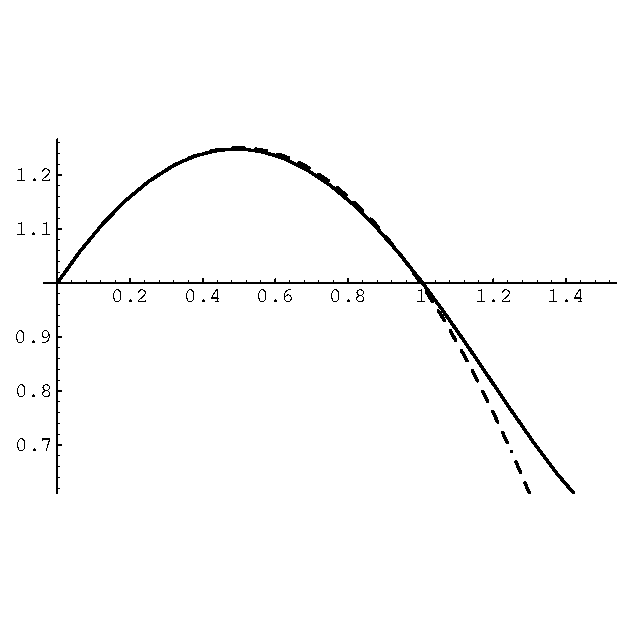
\includegraphics[width=0.4\textwidth]{ode/series/ndsftc}
    \end{center}
    \caption{Plot of the numerical solution and the first three terms in the
      Taylor series.}
    \label{ndsftc}
  \end{figure}
\end{Example}











The general recurrence relation for the $a_n$'s is useful if you only want to
calculate the first few terms in the Taylor expansion.  However,
for many problems substituting the Taylor series for the 
coefficient functions into the differential equation will enable you to 
find a simpler form of the solution.
We consider the following example to illustrate this point.





\begin{Example}
  Develop a series expansion of the solution to the initial value problem
  \[ w'' + \frac{1}{(z^2+1)} w = 0, \qquad w(0) = 1, \quad w'(0) = 0.\]

  \paragraph{Solution using the General Recurrence Relation.}
  The coefficient function has the Taylor expansion
  \[ \frac{1}{1+z^2} = \sum_{n=0}^\infty (-1)^n z^{2n}. \]
  From the initial condition we obtain $a_0 = 1$ and $a_1 = 0$.
  Thus we see that the solution is
  \[ w = \sum_{n=0}^\infty a_n z^n, \]
  where
  \[ a_{n+2} = -\frac{1}{(n+1)(n+2)} \sum_{m=0}^n a_m q_{n-m} \]
  and 
  \[ q_n =        \begin{cases}
    0 \quad &\mathrm{for odd}\ n \\
    (-1)^{(n/2)} \quad &\mathrm{for even}\ n.
  \end{cases}
  \]
  Although this formula is fine if you only want to calculate the first 
  few $a_n$'s, it is just a tad unwieldy to work with.  Let's see if we
  can get a better expression for the solution.

  \paragraph{Substitute the Taylor Series into the Differential Equation.}
  Substituting a Taylor series for $w$ yields
  \[ \frac{\dd^2}{\dd z^2} \sum_{n=0}^\infty a_n z^n + \frac{1}{(z^2 + 1)}
  \sum_{n=0}^\infty a_n z^n=0. \]
  Note that the algebra will be easier if we multiply by $z^2+1$.  The 
  polynomial $z^2+1$ has only two terms, but the Taylor series for
  $1/(z^2+1)$ has an infinite number of terms.
  \begin{gather*}
    (z^2 + 1)\frac{\dd^2}{\dd z^2} \sum_{n=0}^\infty a_n z^n + \sum_{n=0}^\infty a_n z^n=0\\
    \sum_{n=2}^\infty n(n-1)a_n z^n + \sum_{n=2}^\infty n(n-1)a_n z^{n-2}
    + \sum_{n=0}^\infty a_n z^n = 0 \\
    \sum_{n=0}^\infty n(n-1)a_n z^n
    + \sum_{n=0}^\infty (n+2)(n+1)a_{n+2} z^n
    + \sum_{n=0}^\infty a_n z^n = 0 \\
    \sum_{n=0}^\infty \Big[(n+2)(n+1)a_{n+2} + n(n-1)a_n + a_n \Big] z^n = 0
  \end{gather*}
  Equating powers of $z$ gives us the difference equation
  \[a_{n+2} = - \frac{n^2 - n + 1}{(n+2)(n+1)}a_n, \qquad \mathrm{for}\ n \geq 0.\]
  From the initial conditions we see that $a_0 = 1$ and $a_1 = 0$.  
  All of the odd terms in the series will be zero.  
  For the even terms, it is easier to reformulate the problem with 
  the change of variables 
  $b_n = a_{2n}$.  In terms of $b_n$ the difference equation is
  \[ b_{n+1} = - \frac{(2n)^2 - 2n + 1}{(2n+2)(2n+1)}b_{n}, \qquad b_0 = 1.\]
  This is a first order difference equation with the solution
  \[b_n = \prod_{j=0}^n \left(- \frac{4j^2 - 2j + 1}{(2j+2)(2j+1)}\right).\]
  Thus we have that
  \[a_n = 
  \begin{cases}
    \prod_{j=0}^{n/2} \left(- \frac{4j^2 - 2j + 1}{(2j+2)(2j+1)}\right)
    \quad &\mathrm{for even}\ n, \\
    0 & \mathrm{for odd}\  n.
  \end{cases}
  \]

  Note that the nearest singularities of $1/(z^2+1)$ in the complex plane are
  at $z = \pm i$.  Thus the radius of convergence must be at
  least $1$. 
  Applying the ratio test, the series converges for values of $|z|$ such that
  \begin{gather*}
    \lim_{n \to \infty} \left| \frac{a_{n+2} z^{n+2}}{a_n z^n}\right| < 1 \\
    \lim_{n \to \infty} \left| - \frac{n^2 - n + 1}{(n+2)(n+1)}\right| |z|^2
    < 1 \\
    |z|^2 < 1.
  \end{gather*}
  The radius of convergence is $1$.

  The first few terms in the Taylor expansion are
  \[ \boxed{ w = 1 - \frac{1}{2} z^2 + \frac{1}{8} z^4- \frac{13}{240}z^6 
    + \cdots.}\]

  In Figure~\ref{taylor_conv} the plot of the first two nonzero 
  terms is shown in a short
  dashed line, the plot of the first four nonzero terms is shown in a long dashed
  line, and the numerical solution is shown in a solid line.

  \begin{figure}[tb!]
    \begin{center} 
      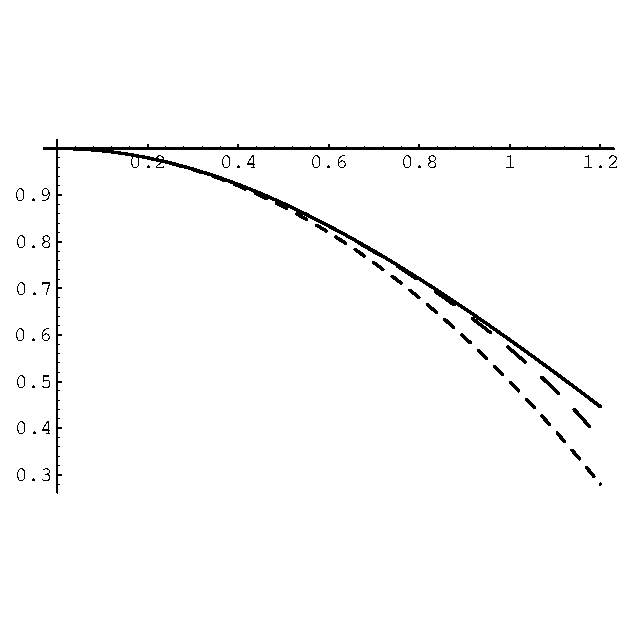
\includegraphics[width=0.4\textwidth]{ode/series/conv1}
    \end{center}
    \caption{Plot of the solution and approximations.}
    \label{taylor_conv}
  \end{figure}

\end{Example}











In general, if the coefficient functions are rational functions, that is
they are fractions of polynomials, multiplying the equations
by the quotient will reduce the algebra involved in finding the series
solution.




\begin{Example}
  If we were going to find the Taylor series expansion about $z=0$
  of the solution to
  \[ w'' + \frac{z}{1+z} w' + \frac{1}{1-z^2} w = 0,\]
  we would first want to multiply the equation by $1-z^2$ to obtain
  \[ (1-z^2) w'' + z (1-z) w'' + w = 0. \]
\end{Example}

























\begin{Example}
  Find the series expansions about $z=0$ of the fundamental set of solutions
  for
  \[ w'' +z^2 w = 0. \]
  Recall that the fundamental set of solutions $\{w_1, w_2\}$ satisfy
  \begin{alignat*}{2}
    w_1(0) &= 1 &\qquad w_2(0) &= 0 \\
    w_1'(0) &= 0 & \qquad w_2'(0) &= 1.
  \end{alignat*}
  Thus if
  \[ w_1 = \sum_{n=0}^\infty a_n z^n \qquad \mathrm{and} \qquad
  w_2 = \sum_{n=0}^\infty b_n z^n,\]
  then the coefficients must satisfy
  \[ a_0 = 1, \quad a_1 = 0, \qquad \mathrm{and} \qquad b_0=0, \quad b_1=1.\]

  Substituting the Taylor expansion $w = \sum_{n=0}^\infty c_n z^n$ into
  the differential equation,
  \begin{gather*}
    \sum_{n=2}^\infty n(n-1)c_n z^{n-2} + \sum_{n=0}^\infty c_n z^{n+2} = 0 \\
    \sum_{n=0}^\infty (n+2)(n+1) c_{n+2} z^n + \sum_{n=2}^\infty c_{n-2}z^n = 0 \\
    2c_2 + 6 c_3 z + \sum_{n=2}^\infty \Big[(n+2)(n+1)c_{n+2} + c_{n-2}\Big]z^n = 0
  \end{gather*}
  Equating coefficients of powers of $z$,
  \begin{alignat*}{2}
    &z^0: & \quad &c_2 = 0 \\
    &z^1: &\quad &c_3 = 0 \\
    &z^n: &\quad &(n+2)(n+1)c_{n+2} + c_{n-2} = 0, 
    \quad \mathrm{for}\ n \geq 2 \\
    &       &    &c_{n+4} = -\frac{c_n}{(n+4)(n+3)}
  \end{alignat*}

  For our first solution we have the difference equation
  \[ a_0 = 1,\ a_1 = 0,\ a_2 = 0,\ a_3 = 0, \qquad 
  a_{n+4} = -\frac{a_n}{(n+4)(n+3)}.\]
  For our second solution,
  \[ b_0 = 0,\ b_1 = 1,\ b_2 = 0,\ b_3 = 0, \qquad 
  b_{n+4} = -\frac{b_n}{(n+4)(n+3)}.\]
  The first few terms in the fundamental set of solutions are
  \[
  \boxed{
    w_1 = 1 - \frac{1}{12} z^4 + \frac{1}{672} z^8 - \cdots, \qquad 
    w_2 = z - \frac{1}{20} z^5 + \frac{1}{1440} z^9 - \cdots.
    }
  \]

  In Figure~\ref{w_one_two} the five term approximation is graphed
  in a coarse dashed line, the ten term approximation is graphed
  in a fine dashed line, and the numerical solution of $w_1$ is graphed in 
  a solid line.
  The same is done for $w_2$.

  \begin{figure}[tb!]
    \begin{center}
      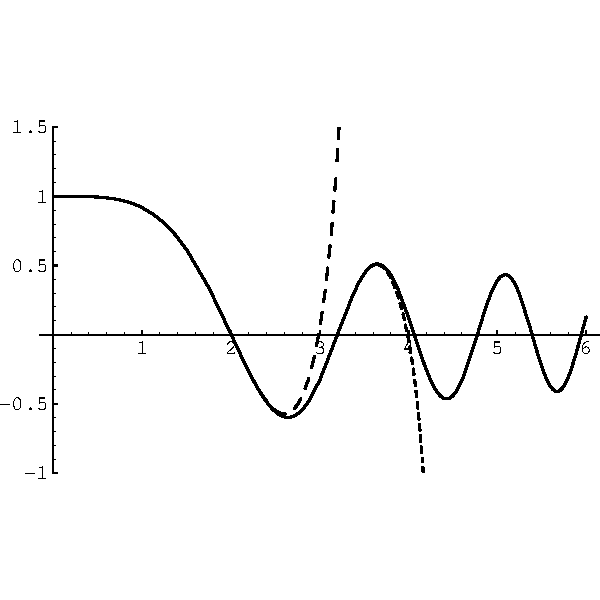
\includegraphics[width=0.4\textwidth]{ode/series/w_one}
      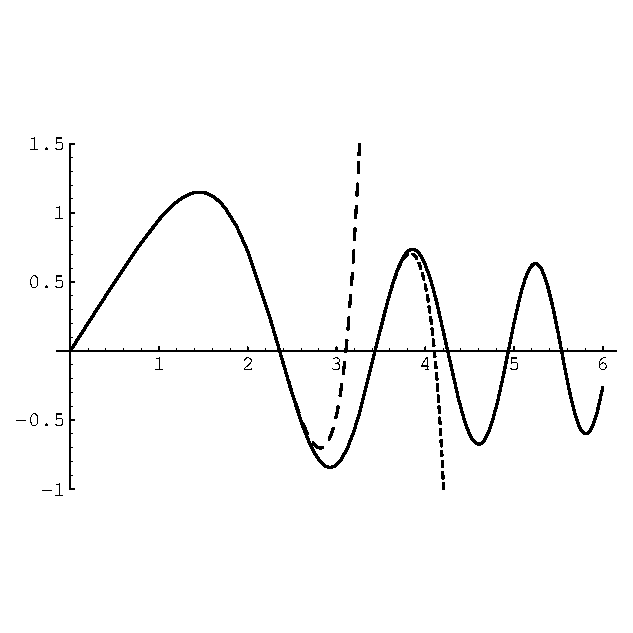
\includegraphics[width=0.4\textwidth]{ode/series/w_two}
    \end{center}
    \caption{The graph of the approximations and the numerical solution.}
    \label{w_one_two}
  \end{figure}


\end{Example}






\begin{Result}
  Consider the $n^{t h}$ order linear homogeneous equation
  \[ \frac{d^n w}{dz^n} + p_{n-1}(z) \frac{d^{n-1}w}{dz^{n-1}} + \cdots
  + p_1(z) \frac{\dd w}{\dd z} + p_0(z) w  = 0.\]
  If each of the coefficient functions $p_i(z)$ are analytic at $z=z_0$
  then $z_0$ is an ordinary point of the differential equation.
  The solution is analytic in some region containing $z_0$ and can
  be expanded in a Taylor series.  The radius of convergence of the
  series will be at least the distance to the nearest singularity of
  the coefficient functions in the complex plane.
\end{Result}
















%%===========================================================================
\section{Regular Singular Points of Second Order Equations}
Consider the differential equation
\[ w'' + \frac{p(z)}{z-z_0} w' + \frac{q(z)}{(z-z_0)^2} w = 0.\]
If $z=z_0$ is not an ordinary point but both $p(z)$ and $q(z)$ are 
analytic at $z=z_0$ then $z_0$ is a \textbf{regular singular point} of the 
differential equation.  The following equations have a regular singular
point at $z=0$.
\begin{itemize}
\item $w'' + \frac{1}{z} w' + z^2 w = 0$
\item $w'' + \frac{1}{\sin z} w' - w = 0$
\item $w'' - z w' + \frac{1}{z \sin z} w = 0$
\end{itemize}

Concerning regular singular points of second order linear equations there
is good news and bad news.

\paragraph{The Good News.} We will find that with the use of the Frobenius 
method we can always find series expansions
of two linearly independent solutions at a regular singular point.  
We will illustrate this theory with several examples.

\paragraph{The Bad News.} Instead of a tidy little theory like we have for 
ordinary points, the solutions can be of several different forms.
Also, for some of the problems the algebra can get pretty ugly.




\begin{Example}
  Consider the equation
  \[w'' + \frac{3(1+z)}{16z^2}w = 0.\]
  We wish to find series solutions about the point $z = 0$.  First we try
  a Taylor series $w = \sum_{n=0}^\infty a_n z^n$.
  Substituting this into the differential equation,
  \begin{gather*}
    z^2 \sum_{n=2}^\infty n(n-1)a_n z^{n-2} 
    + \frac{3}{16}(1+z) \sum_{n=0}^\infty a_n z^n = 0 \\
    \sum_{n=0}^\infty n(n-1)a_n z^n + \frac{3}{16} \sum_{n=0}^\infty a_n z^n
    + \frac{3}{16} \sum_{n=1}^\infty a_{n+1}z^n = 0.
  \end{gather*}
  Equating powers of $z$,
  \begin{alignat*}{2}
    &z^0: &\qquad &a_0 = 0 \\
    &z^n: &\qquad & \left[n(n-1) + \frac{3}{16}\right]a_n + \frac{3}{16} a_{n+1} 
    = 0 \\
    &       &       &a_{n+1} = \left[\frac{16}{3}n(n-1) + 1\right]a_n.
  \end{alignat*}
  This difference equation has the solution $a_n=0$ for all $n$.  Thus we have
  obtained only the trivial solution to the differential equation.  We must
  try an expansion of a more general form.  We recall that for regular singular
  points of first order equations we can always find a solution in the form
  of a Frobenius series $w = z^\alpha \sum_{n=0}^\infty a_n z^n$, $a_0\neq 0$.
  We substitute this series into the differential equation.
  \begin{gather*}
    z^2 \sum_{n=0}^\infty \big[\alpha(\alpha-1)+ 2 \alpha  n + n(n-1) \big] 
    a_n z^{n + \alpha - 2}
    + \frac{3}{16}(1+z)z^\alpha \sum_{n=0}^\infty a_n z^n = 0 \\
    \sum_{n=0}^\infty \big[\alpha(\alpha-1) + 2 n + n(n-1)\big]a_n z^n
    + \frac{3}{16} \sum_{n=0}^\infty a_n z^n
    + \frac{3}{16} \sum_{n=1}^\infty a_{n-1} z^n = 0 
  \end{gather*}
  Equating the $z^0$ term to zero yields the equation
  \[ \left(\alpha(\alpha-1) + \frac{3}{16}\right)a_0 = 0.\]
  Since we have assumed that $a_0\neq 0$, the polynomial in $\alpha$ must
  be zero.  The two roots of the polynomial are
  \[ \alpha_1 = \frac{1+\sqrt{1 - 3/4}}{2} = \frac{3}{4}, \qquad
  \alpha_2 = \frac{1-\sqrt{1 - 3/4}}{2} = \frac{1}{4}.\]
  Thus our two series solutions will be of the form
  \[ w_1 = z^{3/4}\sum_{n=0}^\infty a_n z^n, \qquad
  w_2 = z^{1/4}\sum_{n=0}^\infty b_n z^n.\]

  Substituting the first series into the differential equation,
  \begin{gather*}
    \sum_{n=0}^\infty \left[-\frac{3}{16} + 2n + n(n-1) + \frac{3}{16}\right]a_n z^n
    + \frac{3}{16} \sum_{n=1}^\infty a_{n-1} z^n = 0. 
  \end{gather*}
  Equating powers of $z$, we see that $a_0$ is arbitrary and
  \[ a_n = - \frac{3}{16n(n+1)} a_{n-1} \quad \mathrm{for}\ n \geq 1.\]
  This difference equation has the solution
  \begin{align*} 
    a_n &= a_0 \prod_{j=1}^n \left(-\frac{3}{16j(j+1)}\right) \\
    &= a_0 \left(-\frac{3}{16}\right)^n \prod_{j=1}^n \frac{1}{j(j+1)} \\
    &= a_0 \left(-\frac{3}{16}\right)^n \frac{1}{n!(n+1)!} 
    \quad \mathrm{for}\ n \geq 1.
  \end{align*}

  Substituting the second series into the differential equation,
  \begin{gather*}
    \sum_{n=0}^\infty \left[-\frac{3}{16} + 2n + n(n-1) + \frac{3}{16}\right]b_n z^n
    + \frac{3}{16} \sum_{n=1}^\infty b_{n-1} z^n = 0. 
  \end{gather*}
  We see that the difference equation for $b_n$ is the same as the 
  equation for $a_n$.  Thus we can write the general solution to the 
  differential equation as
  \[w = c_1 z^{3/4} \left(1 + \sum_{n=1}^\infty 
    \left(-\frac{3}{16}\right)^n \frac{1}{n!(n+1)!} z^n \right)
  + c_2 z^{1/4} \left(1 + \sum_{n=1}^\infty 
    \left(-\frac{3}{16}\right)^n \frac{1}{n!(n+1)!} z^n \right) \]
  \[ \boxed{ \left(c_1 z^{3/4} + c_2 z^{1/4}\right) \left(1 + \sum_{n=1}^\infty 
      \left(-\frac{3}{16}\right)^n \frac{1}{n!(n+1)!} z^n \right).}\]
\end{Example}











\subsection{Indicial Equation}
\index{indicial equation}
Now let's consider the general equation for a regular singular point at
$z = 0$
\[ w'' + \frac{p(z)}{z} w' + \frac{q(z)}{z^2} w = 0.\]
Since $p(z)$ and $q(z)$ are analytic at $z=0$ we can expand them in
Taylor series.
\[ p(z) = \sum_{n=0}^\infty p_n z^n, 
\qquad q(z) = \sum_{n=0}^\infty q_n z^n \]
Substituting a Frobenius series $w = z^\alpha \sum_{n=0}^\infty a_n z^n,\ 
a_0 \neq 0$ and the Taylor series for $p(z)$ and $q(z)$ into the differential
equation yields
\[\sum_{n=0}^\infty \Big[(\alpha+n)(\alpha+n-1)\Big]a_n z^n
+ \left(\sum_{n=0}^\infty p_n z^n\right)
\left(\sum_{n=0}^\infty (\alpha+n) a_n z^n\right)
+ \left(\sum_{n=0}^\infty q_n z^n\right)\left(\sum_{n=0}^\infty a_n z^n\right) = 0\]
\begin{align*}
  &\sum_{n=0}^\infty \Big[(\alpha+n)^2 - (\alpha+n) + p_0(\alpha+n)+q_0 \Big]a_n z^n \\
  &\qquad \qquad \qquad + \left(\sum_{n=1}^\infty p_n z^n\right)
  \left(\sum_{n=0}^\infty (\alpha+n) a_n z^n\right)
  + \left(\sum_{n=1}^\infty q_n z^n\right)\left(\sum_{n=0}^\infty a_n z^n\right) = 0
\end{align*}
\[\sum_{n=0}^\infty \Big[(\alpha+n)^2 + (p_0-1)(\alpha_n) + q_0 \Big]a_n z^n
+ \sum_{n=1}^\infty \left( \sum_{j=0}^{n-1} (\alpha+j) a_j p_{n-j}
\right) z^n
+ \sum_{n=1}^\infty \left( \sum_{j=0}^{n-1} a_j q_{n-j} \right) z^n = 0\]


Equating powers of $z$,
\begin{alignat*}{2}
  &z^0: &\quad    &\Big[\alpha^2 + (p_0-1)\alpha + q_0\Big]a_0 = 0 \\
  &z^n: &\quad    &\Big[(\alpha+n)^2 + (p_0-1)(\alpha+n) + q_0\Big]a_n
  = -\sum_{j=0}^{n-1}\Big[(\alpha+j)p_{n-j} + q_{n-j}\Big]a_j.
\end{alignat*}
Let
\[ I(\alpha) = \alpha^2 + (p_0-1)\alpha + q_0 = 0.\]
This is known as the \textbf{indicial equation}.  
The indicial equation gives us the 
form of the solutions.  
The equation for $a_0$ is $I(\alpha)a_0 = 0$.  Since we assumed that $a_0$
is nonzero, $I(\alpha) = 0$.  Let the two roots of $I(\alpha)$ be 
$\alpha_1$ and $\alpha_2$ where $\Re(\alpha_1) \geq \Re(\alpha_2)$.

Rewriting the difference equation for $a_n(\alpha)$,
\begin{equation} \label{diff-a_n}
  I(\alpha+n)a_n(\alpha) 
  = - \sum_{j=0}^{n-1}\Big[(\alpha+j)p_{n-j} + q_{n-j}\Big]a_j(\alpha)
  \quad \mathrm{for}\ n \geq 1.
\end{equation}

If the roots are distinct and do not differ by an integer
then we can use Equation~\ref{diff-a_n} to solve for $a_n(\alpha_1)$
and $a_n(\alpha_2)$, which will give us the two solutions
\[ w_1 = z^{\alpha_1} \sum_{n=0}^\infty a_n(\alpha_1)z^n, \quad \mathrm{and} \quad
w_2 = z^{\alpha_2} \sum_{n=0}^\infty a_n(\alpha_2)z^n.\]

If the roots are not distinct, $\alpha_1 = \alpha_2$, we will only have one
solution and will have to generate another.  If the roots differ by an
integer, $\alpha_1 - \alpha_2 = N$, there is one solution corresponding
to $\alpha_1$, but when we try to solve Equation~\ref{diff-a_n} for 
$a_n(\alpha_2)$, we will encounter the equation
\[ I(\alpha_2 + N)a_N(\alpha_2) = I(\alpha_1)a_N(\alpha_2) 
= 0 \cdot a_N(\alpha_2)
= -\sum_{j=0}^{N-1}\Big[(\alpha+n)p_{n-j} + q_{n-j}\Big]a_j(\alpha_2).\]
If the right side of the equation is nonzero, then $a_N(\alpha_2)$ is
undefined.  On the other hand, 
if the right side is zero then $a_N(\alpha_2)$ is arbitrary.
The rest of this section is devoted to considering the cases 
$\alpha_1 = \alpha_2$ and $\alpha_1 - \alpha_2 = N$.

























\subsection{The Case: Double Root}
Consider a second order equation $L[w] = 0$ with a regular singular point
at $z = 0$.  Suppose the indicial equation has a double root.
\[ I(\alpha) = (\alpha-\alpha_1)^2 = 0\]
One solution has the form
\[ w_1 = z^{\alpha_1} \sum_{n=0}^\infty a_n z^n.\]
In order to find the second solution, we will differentiate with respect to the 
parameter, $\alpha$.  Let $a_n(\alpha)$ satisfy Equation~\ref{diff-a_n}
Substituting the Frobenius expansion into the differential equation,
\[ L\left[z^\alpha \sum_{n=0}^\infty a_n(\alpha) z^n\right] = 0.\]
Setting $\alpha=\alpha_1$ will make the left hand side of the equation zero.
Differentiating this equation with respect to $\alpha$,
\[ \frac{\partial}{\partial \alpha}L\left[z^\alpha \sum_{n=0}^\infty a_n(\alpha) z^n\right] 
= 0.\]
Interchanging the order of differentiation,
\[ L\left[ \log z\,z^\alpha \sum_{n=0}^\infty a_n(\alpha) z^n
  + z^\alpha \sum_{n=0}^\infty \frac{\dd a_n(\alpha)}{\dd \alpha} z^n \right]
= 0.\]
Since setting $\alpha = \alpha_1$ will make the left hand side of this 
equation zero, the second linearly independent solution is
\[ w_2 = \log z\, z^{\alpha_1} \sum_{n=0}^\infty a_n(\alpha_1) z^n
+ z^{\alpha_1} \sum_{n=0}^\infty \frac{\dd a_n(\alpha)}{\dd \alpha} 
\Bigg|_{\alpha=\alpha_1} z^n  \]
\[ \boxed{ w_2 = w_1 \log z
  + z^{\alpha_1} \sum_{n=0}^\infty a_n'(\alpha_1)
  z^n .} \]













\begin{Example}
  Consider the differential equation
  \[ w'' + \frac{1+z}{4z^2} w = 0.\]
  There is a regular singular point at $z = 0$.  The indicial equation is
  \[ \alpha(\alpha-1) + \frac{1}{4} = \left(\alpha-\frac{1}{2}\right)^2 = 0.\]
  One solution will have the form
  \[ w_1 = z^{1/2} \sum_{n=0}^\infty a_n z^n , \quad a_0 \neq 0.\]

  Substituting the Frobenius expansion
  \[z^\alpha \sum_{n=0}^\infty a_n(\alpha) z^n\]
  into the differential equation yields
  \begin{gather*}
    z^2 w'' + \frac{1}{4}(1+z) w = 0 \\
    \sum_{n=0}^\infty \big[\alpha(\alpha-1) + 2 \alpha n + n(n-1)  \big]
    a_n(\alpha) z^{n+\alpha}
    + \frac{1}{4} \sum_{n=0}^\infty a_n(\alpha) z^{n+\alpha}
    + \frac{1}{4} \sum_{n=0}^\infty a_n(\alpha) z^{n+\alpha+1} = 0. \\
    \intertext{Divide by $z^\alpha$ and adjust the summation indices.}
    \sum_{n=0}^\infty \left[\alpha(\alpha-1) + 2 \alpha n + n(n-1)  \right]
    a_n(\alpha) z^n
    + \frac{1}{4} \sum_{n=0}^\infty a_n(\alpha) z^n
    + \frac{1}{4} \sum_{n=1}^\infty a_{n-1}(\alpha) z^n = 0 \\
    \left[\alpha(\alpha-1)a_0 + \frac{1}{4}\right]a_0
    + \sum_{n=1}^\infty \left(\left[\alpha(\alpha-1) + 2 n + n(n-1) 
        + \frac{1}{4}\right]a_n(\alpha) + \frac{1}{4} a_{n-1}(\alpha)
    \right) z^n=0
  \end{gather*}
  Equating the coefficient of $z^0$ to zero yields $I(\alpha) a_0 = 0$.
  Equating the coefficients of $z^n$ to zero yields the difference equation
  \begin{gather*}
    \left[\alpha(\alpha-1) + 2 n + n(n-1) 
      + \frac{1}{4}\right]a_n(\alpha) + \frac{1}{4} a_{n-1}(\alpha) = 0 \\
    a_n(\alpha) = - \left(\frac{n(n+1)}{4} + \frac{\alpha(\alpha-1)}{4} 
      + \frac{1}{16} \right)a_{n-1}(\alpha).
  \end{gather*}
  The first few $a_n$'s are
  \[ a_0,\quad -\left(\alpha(\alpha-1) + \frac{9}{16} \right)a_0, \quad
  \left(\alpha(\alpha-1) + \frac{25}{16} \right)
  \left(\alpha(\alpha-1) + \frac{9}{16} \right)a_0,\ldots \]
  Setting $\alpha=1/2$, the coefficients for the first solution are
  \[a_0,\quad  -\frac{5}{16} a_0,\quad \frac{105}{16}a_0,\quad \ldots\]

  The second solution has the form
  \[ w_2 = w_1 \log z 
  + z^{1/2} \sum_{n=0}^\infty a_n'(1/2) z^n.\]
  Differentiating the $a_n(\alpha)$, 
  \[ \frac{\dd a_0}{\dd \alpha} = 0, 
  \quad  \frac{\dd a_1(\alpha)}{\dd \alpha} = -(2\alpha - 1)a_0,\quad  
  \frac{\dd a_2(\alpha)}{\dd \alpha} = 
  (2\alpha-1)\left[\left(\alpha(\alpha-1) + \frac{9}{16} \right)+ 
    \left(\alpha(\alpha-1) + \frac{25}{16} \right)
  \right]a_0,\quad \ldots\]
  Setting $\alpha = 1/2$ in this equation yields
  \[ a_0' = 0,\quad a_1'(1/2) = 0,\quad a_2'(1/2) = 0,\quad \ldots\]
  Thus the second solution is
  \[ w_2 = w_1 \log z .\]
  The first few terms in the general solution are
  \[ \boxed{(c_1 + c_2 \log z)\left(1 - \frac{5}{16}z + \frac{105}{16}z^2 
      - \cdots \right).}\]
\end{Example}














\subsection{The Case: Roots Differ by an Integer}
Consider the case in which the roots of the indicial equation $\alpha_1$
and $\alpha_2$ differ by an integer. ($\alpha_1 - \alpha_2 = N$) 
Recall the equation that determines $a_n(\alpha)$ 
\[ I(\alpha+n)a_n = \Big[(\alpha+n)^2 + (p_0-1)(\alpha+n)+q_0\Big]a_n 
= - \sum_{j=0}^{n-1} \Big[(\alpha+j)p_{n-j} + q_{n-j}\Big]a_j.\]
When $\alpha = \alpha_2$ the equation for $a_N$ is
\[ I(\alpha_2 + N) a_N(\alpha_2) = 0 \cdot a_N(\alpha_2)  
= - \sum_{j=0}^{N-1} \Big[(\alpha+j)p_{N-j} + q_{N-j}\Big]a_j.\]
If the right hand side of this equation is zero, then $a_N$ is arbitrary.
There will
be two solutions of the Frobenius form.
\[ w_1 = z^{\alpha_1} \sum_{n=0}^\infty a_n(\alpha_1) z^n \quad \mathrm{and} \quad
w_2 = z^{\alpha_2} \sum_{n=0}^\infty a_n(\alpha_2) z^n.\]
If the right hand side of the equation is nonzero
then $a_N(\alpha_2)$ will be undefined.
We will have to generate the second solution.  Let
\[ w(z,\alpha) = z^\alpha \sum_{n=0}^\infty a_n(\alpha) z^n,\]
where $a_n(\alpha)$ satisfies the recurrence formula.
Substituting this series into the differential equation yields
\[ L[w(z,\alpha)] = 0.\]
We will multiply by $(\alpha-\alpha_2)$, 
differentiate this equation with respect to $\alpha$ and then set
$\alpha = \alpha_2$.  This will generate a linearly independent solution.
\begin{align*}
  \frac{\partial}{\partial \alpha} L[(\alpha-\alpha_2) w(z, \alpha)]
  &= L\left[ \frac{\partial}{\partial \alpha} (\alpha-\alpha_2)w(z,\alpha) \right] \\
  &= L\left[ \frac{\partial}{\partial \alpha} (\alpha-\alpha_2)
    z^\alpha \sum_{n=0}^\infty a_n(\alpha) z^n \right] \\
  &= L\left[ \log z\ z^\alpha \sum_{n=0}^\infty (\alpha-\alpha_2)a_n(\alpha)z^n
    +z^\alpha \sum_{n=0}^\infty \frac{\dd}{\dd \alpha} [(\alpha-\alpha_2)
    a_n(\alpha)] z^n \right]
\end{align*}
Setting $\alpha = \alpha_2$ with make this expression zero, thus
\[ \log z\ z^\alpha \sum_{n=0}^\infty \lim_{\alpha \to \alpha_2} 
\left\{ (\alpha-\alpha_2)a_n(\alpha) \right\} z^n
+z^{\alpha_2} \sum_{n=0}^\infty \lim_{\alpha \to \alpha_2} \left\{
  \frac{\dd}{\dd \alpha} [(\alpha-\alpha_2)a_n(\alpha)] \right\} z^n \]
is a solution.
Now let's look at the first term in this solution
\[ \log z\ z^\alpha \sum_{n=0}^\infty \lim_{\alpha \to \alpha_2}
\left\{ (\alpha-\alpha_2)a_n(\alpha) \right\} z^n. \]
The first $N$ terms in the sum will be zero.   
That is because $a_0, \ldots, a_{N-1}$ are finite, so multiplying by 
$(\alpha-\alpha_2)$ and taking the limit as $\alpha \to \alpha_2$ will make
the coefficients vanish.
The equation for $a_N(\alpha)$ is
\[ I(\alpha + N) a_N(\alpha) 
= - \sum_{j=0}^{N-1} \Big[(\alpha+j)p_{N-j} + q_{N-j}\Big]a_j(\alpha). \]
Thus the coefficient of the $N^{t h}$ term is
\begin{align*}
  \lim_{\alpha \to \alpha_2}(\alpha-\alpha_2)a_N(\alpha)
  &= -\lim_{\alpha \to \alpha_2} \left[ \frac{(\alpha-\alpha_2)}
    {I(\alpha+N)}\sum_{j=0}^{N-1} 
    \Big[(\alpha+j)p_{N-j} + q_{N-j}\Big]a_j(\alpha) \right]\\
  &= -\lim_{\alpha \to \alpha_2} \left[ \frac{(\alpha-\alpha_2)}
    {(\alpha + N - \alpha_1)(\alpha+N-\alpha_2)}\sum_{j=0}^{N-1} 
    \Big[(\alpha+j)p_{N-j} + q_{N-j}\Big]a_j(\alpha) \right]\\
  \intertext{Since $\alpha_1 = \alpha_2 + N$, $\lim_{\alpha \to \alpha_2} 
    \frac{\alpha-\alpha_2}{\alpha+N-\alpha_1} = 1$.}
  &= -\frac{1}{(\alpha_1 - \alpha_2)}\sum_{j=0}^{N-1} 
  \Big[(\alpha_2+j)p_{N-j} + q_{N-j}\Big]a_j(\alpha_2) .
\end{align*}
Using this you can show that the first term in the solution can be written
\[ d_{-1} \log z\ w_1, \]
where $d_{-1}$ is a constant.
Thus the second linearly independent solution is
\[ \boxed{ w_2 = d_{-1} \log z\ w_1 + 
  z^{\alpha_2} \sum_{n=0}^\infty d_n z^n, } \]
where
\[ d_{-1} = - \frac{1}{a_0} 
\frac{1}{(\alpha_1 - \alpha_2)}\sum_{j=0}^{N-1}
\Big[(\alpha_2+j)p_{N-j} + q_{N-j}\Big]a_j(\alpha_2) \]
and
\[ d_n = \lim_{\alpha \to \alpha_2} \left\{
  \frac{\dd}{\dd \alpha} \Big[(\alpha-\alpha_2)a_n(\alpha)\Big] \right\} 
\quad \mathrm{for}\ n \geq 0. \]













\begin{Example}
  Consider the differential equation
  \[ w'' + \left(1 - \frac{2}{z} \right) w' + \frac{2}{z^2} w = 0. \]
  The point $z = 0$ is a regular singular point.  In order to find series
  expansions of the solutions, we first calculate the indicial equation.
  We can write the coefficient functions in the form
  \[ \frac{p(z)}{z} = \frac{1}{z}(-2 + z), \quad \mathrm{and} \quad
  \frac{q(z)}{z^2} = \frac{1}{z^2}(2). \]
  Thus the indicial equation is
  \begin{gather*}
    \alpha^2 + (-2-1)\alpha + 2 = 0 \\
    (\alpha-1)(\alpha-2) = 0.
  \end{gather*}

  \paragraph{The First Solution.}
  The first solution will have the Frobenius form
  \[ w_1 = z^2 \sum_{n=0}^\infty a_n(\alpha_1) z^n. \]
  Substituting a Frobenius series into the differential equation,
  \begin{gather*}
    z^2 w'' + (z^2 - 2z) w' + 2 w = 0 \\
    \sum_{n=0}^\infty (n + \alpha)(n + \alpha-1) z^{n+\alpha}
    + (z^2-2z) \sum_{n=0}^\infty (n+\alpha)z^{n+\alpha-1}
    + 2 \sum_{n=0}^\infty a_n z^n = 0 \\
    [\alpha^2 - 3 \alpha + 2]a_0 + \sum_{n=1}^\infty \Big[(n+\alpha)(n+\alpha-1)a_n 
    + (n + \alpha-1)a_{n-1}
    -2 (n+\alpha)a_n + 2a_n\Big] z^n = 0.
  \end{gather*}
  Equating powers of $z$,
  \begin{gather*}
    \Big[(n+\alpha)(n+\alpha-1)  -2 (n+\alpha) + 2\Big] a_n = - (n + \alpha-1)a_{n-1} \\
    a_n = - \frac{a_{n-1}}{n+\alpha-2} . 
  \end{gather*}

  Setting $\alpha = \alpha_1 = 2$, the recurrence relation becomes
  \begin{align*}
    a_n(\alpha_1) &= - \frac{a_{n-1}(\alpha_1)}{n} \\
    &= a_0 \frac{(-1)^n}{n!}. 
  \end{align*}
  The first solution is
  \[ \boxed{ w_1 = a_0 \sum_{n=0}^\infty \frac{(-1)^n}{n!} z^n 
    = a_0 \e^{-z}.} \]

  \paragraph{The Second Solution.}
  The equation for $a_1(\alpha_2)$ is
  \[ 0 \cdot a_1(\alpha_2) = 2 a_0. \]
  Since the right hand side of this equation is not 
  zero, the second solution will
  have the form
  \[ w_2 = d_{-1} \log z\ w_1 + 
  z^{\alpha_2} \sum_{n=0}^\infty \lim_{\alpha \to \alpha_2} \left\{
    \frac{\dd}{\dd \alpha} [(\alpha-\alpha_2)a_n(\alpha)] \right\}z^n \]

  First we will calculate $d_{-1}$ as we defined it previously.
  \[ d_{-1} = - \frac{1}{a_0} \frac{1}{2-1} a_0 = -1. \]
  The expression for $a_n(\alpha)$ is
  \[ a_n(\alpha) = \frac{(-1)^n a_0}{(\alpha+n-2)(\alpha+n-1) 
    \cdots(\alpha-1)}. \]
  The first few $a_n(\alpha)$ are
  \begin{align*}
    a_1(\alpha) &= - \frac{a_0}{\alpha-1} \\
    a_2(\alpha) &= \frac{a_0}{\alpha(\alpha-1)} \\
    a_3(\alpha) &= -\frac{a_0}{(\alpha+1)\alpha(\alpha-1)}.
  \end{align*}
  We would like to calculate
  \[ d_n = \lim_{\alpha \to 1} \left\{
    \frac{\dd}{\dd \alpha} \Big[(\alpha-1)a_n(\alpha)\Big] \right\}. \]
  The first few $d_n$ are
  \begin{align*}
    d_0     &= \lim_{\alpha \to 1} \left\{
      \frac{\dd}{\dd \alpha} \Big[(\alpha-1) a_0\Big] \right\} \\
    &= a_0 \\
    d_1     &= \lim_{\alpha \to 1} \left\{
      \frac{\dd}{\dd \alpha} \left[(\alpha-1)
        \left( - \frac{a_0}{\alpha-1} \right)\right] \right\} \\
    &= \lim_{\alpha \to 1} \left\{
      \frac{\dd}{\dd \alpha} \Big[-a_0\Big] \right\} \\
    &= 0 \\
    d_2     &= \lim_{\alpha \to 1} \left\{
      \frac{\dd}{\dd \alpha} \left[(\alpha-1)
        \left( \frac{a_0}{\alpha(\alpha-1)} \right)\right] \right\} \\
    &= \lim_{\alpha \to 1} \left\{
      \frac{\dd}{\dd \alpha} \left[\frac{a_0}{\alpha}\right]\right\} \\
    &= -a_0 \\
    d_3     &= \lim_{\alpha \to 1} \left\{
      \frac{\dd}{\dd \alpha} \left[(\alpha-1)
        \left( -\frac{a_0}{(\alpha+1)\alpha(\alpha-1)}
        \right)\right] \right\} \\
    &= \lim_{\alpha \to 1} \left\{
      \frac{\dd}{\dd \alpha} \left[-\frac{a_0}{(\alpha+1)\alpha} \right] \right\} \\
    &= \frac{3}{4}a_0.
  \end{align*}
  It will take a little work to find the general
  expression for $d_n$.  We will need the
  following relations.
  \[ \Gamma(n) = (n-1)!, \quad \Gamma'(z) = \Gamma(z) \psi(z), \quad
  \psi(n) = - \gamma + \sum_{k=1}^{n-1} \frac{1}{k}. \]
  See the chapter on the Gamma function for explanations of these equations.
  \begin{align*}
    d_n     &= \lim_{\alpha \to 1} \left\{
      \frac{\dd}{\dd \alpha} \left[(\alpha-1)
        \frac{(-1)^n a_0 }{(\alpha+n-2)(\alpha+n-1)\cdots(\alpha-1) }\right] 
    \right\} \\
    &= \lim_{\alpha \to 1} \left\{
      \frac{\dd}{\dd \alpha} \left[\frac{(-1)^n a_0 }{(\alpha+n-2)(\alpha+n-1)
          \cdots(\alpha)}\right]\right\} \\
    &= \lim_{\alpha \to 1} \left\{
      \frac{\dd}{\dd \alpha} \left[\frac{(-1)^n a_0 \Gamma(\alpha)}
        {\Gamma(\alpha+n-1)} \right] \right\} \\
    &= (-1)^n a_0 \lim_{\alpha \to 1} \left\{ \frac{\Gamma(\alpha)
        \psi(\alpha)}{\Gamma(\alpha+n-1)} - \frac{\Gamma(\alpha)
        \psi(\alpha+n-1)}{\Gamma(\alpha+n-1)} \right\} \\
    &= (-1)^n a_0 \lim_{\alpha \to 1} \left\{ \frac{\Gamma(\alpha)
        [\psi(\alpha)-\psi(\alpha+n-1)]}{\Gamma(\alpha+n-1)} \right\} \\
    &= (-1)^n a_0 \frac{\psi(1) - \psi(n)}{(n-1)!} \\
    &= \frac{(-1)^{n+1} a_0}{(n-1)!} \sum_{k=0}^{n-1} \frac{1}{k}
  \end{align*}
  Thus the second solution is
  \[ \boxed{ w_2 = -\log z\ w_1 + z \sum_{n=0}^\infty \left( \frac{(-1)^{n+1} a_0}
      {(n-1)!} \sum_{k=0}^{n-1} \frac{1}{k}\right) z^n.} \]
  The general solution is
  \[ \boxed{ w = c_1 \e^{-z} - c_2 \log z\ \e^{-z} + c_2 
    z \sum_{n=0}^\infty \left( \frac{(-1)^{n+1} }
      {(n-1)!} \sum_{k=0}^{n-1} \frac{1}{k}\right) z^n. } \]
\end{Example}


We see that even in problems that are chosen for their simplicity, the algebra
involved in the Frobenius method can be pretty involved.







\begin{Example}
  Consider a series expansion about the origin of the equation
  \[ w'' + \frac{1-z}{z} w' - \frac{1}{z^2} w = 0. \]

  The indicial equation is
  \begin{gather*}
    \alpha^2 -1 = 0 \\
    \alpha = \pm 1.
  \end{gather*}

  Substituting a Frobenius series into the differential equation,
  \begin{gather*}
    z^2 \sum_{n=0}^\infty (n+\alpha)(n+\alpha-1) a_n z^{n-2} + (z-z^2)\sum_{n=0}^\infty (n+\alpha)
    a_n z^{n-1} - \sum_{n=0}^\infty a_n z^n = 0 \\
    \sum_{n=0}^\infty (n+\alpha)(n+\alpha-1) a_n z^n + \sum_{n=0}^\infty (n+\alpha)a_n z^n
    - \sum_{n=1}^\infty (n+\alpha-1)a_{n-1}z^n - \sum_{n=0}^\infty a_n z^n = 0 \\
    \Big[\alpha(\alpha-1) + \alpha - 1\Big] a_0 
    + \sum_{n=1}^\infty \Big[n+\alpha)(n+\alpha-1) a_n
    + (n+\alpha-1) a_n - (n+\alpha-1)a_{n-1}\Big] z^n = 0.
  \end{gather*}
  Equating powers of $z$ to zero,
  \[ a_n(\alpha) = \frac{a_{n-1}(\alpha)}{n+\alpha+1} . \]

  We know that the first solution has the form
  \[ w_1 = z \sum_{n=0}^\infty a_n z^n. \]
  Setting $\alpha = 1$ in the reccurence formula,
  \[ a_n = \frac{a_{n-1}}{n+2} = \frac{2 a_0}{(n+2)!}. \]
  Thus the first solution is
  \begin{align*}
    w_1     &= z \sum_{n=0}^\infty \frac{2 a_0}{(n+2)!} z^n \\
    &= 2 a_0 \frac{1}{z} \sum_{n=0}^\infty \frac{z^{n+2}}{(n+2)!} \\
    &= \frac{2 a_0}{z} \left( \sum_{n=0}^\infty \frac{z^n}{n!} - 1 - z \right) \\
    &= \frac{2 a_0}{z} (\e^z - 1 - z).
  \end{align*}

  Now to find the second solution.  Setting $\alpha = -1$ in the reccurence 
  formula,
  \[ a_n = \frac{a_{n-1}}{n} = \frac{a_0}{n!}. \]
  We see that in this case there is no trouble in defining $a_2(\alpha_2)$.
  The second solution is
  \[ w_2 = \frac{a_0}{z} \sum_{n=0}^\infty \frac{z^n}{n!} = \frac{a_0}{z} \e^z. \]

  Thus we see that the general solution is
  \[ w = \frac{c_1}{z} (\e^z - 1 - z) + \frac{c_2}{z} \e^z \]
  \[ \boxed{ w = \frac{d_1}{z} \e^z + d_2 \left(1+\frac{1}{z} \right). } \]
\end{Example}




































%%===========================================================================
\section{Irregular Singular Points}
\index{irregular singular points}

If a point $z_0$ of a differential equation is not ordinary or regular 
singular, then it is an \textbf{irregular singular point}.
At least one of the solutions at an irregular singular point will not be of
the Frobenius form.  We will examine how to obtain series expansions about
an irregular singular point in the chapter on asymptotic expansions.













%%===========================================================================
\section{The Point at Infinity}
\index{point at infinity!differential equations}

If we want to determine the behavior of a function $f(z)$ at infinity,
we can make the transformation $\zeta = 1 / z$ and examine the point $\zeta = 0$.


\begin{Example}
  Consider the behavior of $f(z) = \sin z$ at infinity.
  This is the same as considering the point $\zeta = 0$ of $\sin(1/\zeta)$, which
  has the series expansion
  \[ 
  \sin \left( \frac{1}{\zeta} \right)
  = \sum_{n=0}^\infty \frac{(-1)^n}{(2 n + 1)! \zeta^{2n+1}}. 
  \]
  Thus we see that the point $\zeta = 0$ is an essential singularity of 
  $\sin(1/\zeta)$.  Hence $\sin z$ has an essential singularity at $z = \infty$.
\end{Example}







\begin{Example}
  Consider the behavior at infinity of $z \e^{1/z}$.  We make the transformation
  $\zeta = 1/z$.
  \[ 
  \frac{1}{\zeta} \e^\zeta = \frac{1}{\zeta} \sum_{n=0}^\infty \frac{\zeta^n}{n!}
  \]
  Thus $z \e^{1/z}$ has a pole of order $1$ at infinity.
\end{Example}






In order to classify the point at infinity of a differential equation
in $w(z)$, we apply the transformation $\zeta = 1/z$, $u(\zeta) = w(z)$.
We write the derivatives with respect to $z$ in terms of $\zeta$.
\begin{align*}
  z &= \frac{1}{\zeta} 
  \\
  \dd z &= - \frac{1}{\zeta^2} \dd \zeta 
  \\
  \frac{\dd}{\dd z} &= - \zeta^2 \frac{\dd}{\dd \zeta}
\end{align*}
\begin{align*}
  \frac{\dd^2}{\dd z^2} &= -\zeta^2 \frac{\dd}{\dd \zeta} \left( - \zeta^2 \frac{\dd}{\dd \zeta} 
  \right) 
  \\
  &= \zeta^4 \frac{\dd^2}{\dd \zeta^2} + 2 \zeta^3 \frac{\dd}{\dd \zeta}
\end{align*}
Now we apply the transformation to the differential equation.
\begin{gather*}
  w'' + p(z) w' + q(z) w = 0
  \\
  \zeta^4 u'' + 2 \zeta^3 u' + p(1/\zeta) (-\zeta^2) u' + q(1/\zeta) u = 0 
  \\
  u'' + \left( \frac{2}{\zeta} - \frac{p(1/\zeta)}{\zeta^2} \right) u'
  + \frac{q(1/\zeta)}{\zeta^4} u = 0
\end{gather*}





\begin{Example}
  Classify the singular points of the differential equation
  \[ 
  w'' + \frac{1}{z} w' + 2 w = 0. 
  \]

  There is a regular singular point at $z = 0$.  To examine the point 
  at infinity
  we make the transformation $\zeta = 1/z$, $u(\zeta) = w(z)$.
  \begin{gather*}
    u'' + \left( \frac{2}{\zeta} - \frac{1}{\zeta} \right) u' + \frac{2}{\zeta^4} u = 0 
    \\
    u'' + \frac{1}{\zeta}  u' + \frac{2}{\zeta^4} u = 0
  \end{gather*}
  Thus we see that the differential equation for $w(z)$ has an irregular 
  singular point at infinity.
\end{Example}






























\raggedbottom
%%===========================================================================
\exercises{
\pagebreak
\flushbottom
\section{Exercises}






%% Hermite equation
\begin{Exercise}[mathematica/ode/series/series.nb]
  \label{exercise hermite eqn}
  $f(x)$ satisfies the Hermite equation
  \[
  \frac{\dd^2 f}{\dd x^2} - 2 x \frac{\dd f}{\dd x} + 2 \lambda f = 0.
  \]
  Construct two linearly independent solutions of the equation as Taylor
  series about $x = 0$.  For what values of $x$ do the series converge?

  Show that for certain values of $\lambda$, called eigenvalues,
  one of the solutions is a polynomial, called an eigenfunction.
  Calculate the first four eigenfunctions $H_0(x)$, $H_1(x)$, $H_2(x)$,
  $H_3(x)$, ordered by degree.

  \hintsolution{hermite eqn}
\end{Exercise}





%% Legendre equation
\begin{Exercise}
  \label{exercise legendre eqn}
  Consider the Legendre equation
  \[
  (1-x^2) y'' - 2 x y' + \alpha (\alpha+1) y = 0.
  \]
  \begin{enumerate}
    %%
  \item
    Find two linearly independent solutions in the form of power series about
    $x = 0$.
    %%
  \item
    Compute the radius of convergence of the series.  Explain why it is possible
    to predict the radius of convergence without actually deriving
    the series.
    %%
  \item
    Show that if $\alpha = 2n$, with $n$ an integer and $n \geq 0$, the series
    for one of the solutions reduces to an even polynomial of degree $2n$.
    %%
  \item
    Show that if $\alpha = 2n+1$, with $n$ an integer and $n \geq 0$, the series
    for one of the solutions reduces to an odd polynomial of degree $2n+1$.
    %%
  \item
    Show that the first 4 polynomial solutions $P_n(x)$ (known as
    \textit{Legendre} polynomials) ordered by their degree and normalized
    so that $P_n(1) = 1$ are
    \begin{alignat*}{2}
      P_0 &= 1 &\quad P_1 &= x \\
      P_2 &= \frac{1}{2} (3 x^2 - 1) &\quad P_4 &= \frac{1}{2} (5 x^3 - 3 x)
    \end{alignat*}
    %%
  \item Show that the Legendre equation can also be written as
    \[ 
    ( (1 - x^2) y^\prime )^\prime = - \alpha (\alpha + 1) y.
    \]
    Note that two Legendre polynomials $P_n(x)$ and $P_m(x)$ must satisfy
    this relation for $\alpha=n$ and $\alpha=m$ respectively. By multiplying
    the first relation by $P_m(x)$ and the second by $P_n(x)$ and integrating
    by parts show that Legendre polynomials satisfy the orthogonality relation
    \[ 
    \int_{-1}^1 P_n(x) P_m(x) \,\dd x = 0\ \mathrm{if}\ n \neq m.
    \] 
    If $n = m$, it can be shown that the value of the integral is $2/(2 n + 1)$. 
    Verify this for the first three polynomials (but you needn't prove it in 
    general).  
  \end{enumerate}

  \hintsolution{legendre eqn}
\end{Exercise}



%%111111111111111111111111111111111111111111111111111111111111111111111111111
\begin{Exercise} 
  \label{exercise w1sinzw1zz2w=0}
  Find the forms of two linearly independent series expansions about the
  point $z = 0$ for the differential equation
  \[ w'' + \frac{1}{\sin z} w' + \frac{1 - z}{z^2}w = 0,\]
  such that the series are real-valued on the positive real axis.
  Do not calculate the coefficients in the expansions.

  \hintsolution{w1sinzw1zz2w=0}
\end{Exercise}



%%222222222222222222222222222222222222222222222222222222222222222222222222222
\begin{Exercise}
  \label{exercise wwz12w=0}
  Classify the singular points of the equation 
  \[ w'' + \frac{w'}{z-1} + 2w = 0. \]

  \hintsolution{wwz12w=0}
\end{Exercise}



%%333333333333333333333333333333333333333333333333333333333333333333333333333
\begin{Exercise}
  \label{exercise w54zwz18zw=0}
  Find the series expansions about $z = 0$ for
  \[      w'' + \frac{5}{4z} w' + \frac{z-1}{8z^2} w = 0. \]

  \hintsolution{w54zwz18zw=0}
\end{Exercise}





%% CONTINUE: Solve the Hermite equation instead.
%%444444444444444444444444444444444444444444444444444444444444444444444444444444
\begin{Exercise}
  \label{exercise wzww=0}
  Find the series expansions about $z = 0$ of the fundamental solutions of 
  \[ 
  w'' + z w' + w = 0. 
  \]

  \hintsolution{wzww=0}
\end{Exercise}





%%555555555555555555555555555555555555555555555555555555555555555555555555555555
\begin{Exercise}
  \label{exercise w12zw1zw=0}
  Find the series expansions about $z=0$
  of the two linearly independent solutions of
  \[ 
  w'' + \frac{1}{2z} w' + \frac{1}{z} w = 0. 
  \]

  \hintsolution{w12zw1zw=0}
\end{Exercise}




%%666666666666666666666666666666666666666666666666666666666666666666666666666666
\begin{Exercise}
  \label{exercise w2z3zw1zw=0}
  Classify the singularity at infinity of the differential equation
  \[ 
  w'' + \left(\frac{2}{z}+ \frac{3}{z^2} \right)w' + \frac{1}{z^2} w = 0. 
  \]
  Find the forms of the series solutions of the differential equation about
  infinity that are real-valued when $z$ is real-valued and positive.  
  Do not calculate the coefficients in the expansions.

  \hintsolution{w2z3zw1zw=0}
\end{Exercise}














%% x \frac{\dd^2 y}{\dd x^2} + (b - x) \frac{\dd y}{\dd x} - a y = 0
\begin{Exercise}
  \label{exercise xybxyay=0}
  Consider the second order differential equation
  \[
  x \frac{\dd^2 y}{\dd x^2} + (b - x) \frac{\dd y}{\dd x} - a y = 0,
  \]
  where $a$, $b$ are real constants.
  \begin{enumerate}
    %%
    %%
  \item
    Show that $x = 0$ is a regular singular point.  Determine the location of
    any additional singular points and classify them.  Include the 
    point at infinity.
    %%
    %%
  \item
    Compute the indicial equation for the point $x = 0$.
    %%
    %%
  \item
    By solving an appropriate recursion relation, show that one solution has
    the form
    \[
    y_1(x) = 1 + \frac{a x}{b} + \frac{ (a)_2 x^2 }{ (b)_2 2! } + \cdots
    + \frac{ (a)_n x^n }{ (b)_n n! } + \cdots
    \]

    where the notation $(a)_n$ is defined by
    \[
    (a)_n = a(a+1)(a+2) \cdots (a+n-1), \quad (a)_0 = 1.
    \]
    Assume throughout this problem that $b \neq n$ where $n$ is a non-negative
    integer.
    %%
    %%
  \item
    Show that when $a = -m$, where $m$ is a non-negative integer, that there are
    polynomial solutions to this equation.  Compute the radius of convergence of 
    the series above when $a \neq -m$.  Verify that the result you get is in 
    accord with the Frobenius theory.
    %%
    %%
  \item
    Show that if $b = n+1$ where $n = 0, 1, 2, \ldots$, then the second 
    solution of this equation has logarithmic terms.  Indicate the \textit{form}
    of the second solution in this case.  You need  not compute any 
    coefficients.
  \end{enumerate}

  \hintsolution{xybxyay=0}
\end{Exercise}




\begin{Exercise}
  \label{exercise xy+2xy+6exy=0}
  Consider the equation
  \[ 
  x y'' + 2 x y' + 6 \e^x y = 0.
  \]
  Find the first three non-zero terms in each of two linearly independent
  series solutions about $x = 0$. 

  \hintsolution{xy+2xy+6exy=0}
\end{Exercise}














\raggedbottom
}
%%===========================================================================
\hints{
\pagebreak
\flushbottom
\section{Hints}






%% Hermite equation
\begin{Hint}
  \label{hint hermite eqn}
  %% CONTINUE
\end{Hint}



%% Legendre equation
\begin{Hint}
  \label{hint legendre eqn}
  %% CONTINUE
\end{Hint}

%%111111111111111111111111111111111111111111111111111111111111111111111111111
\begin{Hint}
  \label{hint w1sinzw1zz2w=0}
  %% CONTINUE
\end{Hint}

%%222222222222222222222222222222222222222222222222222222222222222222222222222
\begin{Hint}
  \label{hint wwz12w=0}
  %% CONTINUE
\end{Hint}


%%333333333333333333333333333333333333333333333333333333333333333333333333333
\begin{Hint}
  \label{hint w54zwz18zw=0}
  %% CONTINUE
\end{Hint}

%%444444444444444444444444444444444444444444444444444444444444444444444444444444
\begin{Hint}
  \label{hint wzww=0}
  %% CONTINUE
\end{Hint}

%%555555555555555555555555555555555555555555555555555555555555555555555555555555
\begin{Hint}
  \label{hint w12zw1zw=0}
  %% CONTINUE
\end{Hint}

%%666666666666666666666666666666666666666666666666666666666666666666666666666666
\begin{Hint}
  \label{hint w2z3zw1zw=0}
  %% CONTINUE
\end{Hint}











%% x \frac{\dd^2 y}{\dd x^2} + (b - x) \frac{\dd y}{\dd x} - a y = 0
\begin{Hint}
  \label{hint xybxyay=0}
  %% CONTINUE
\end{Hint}




\begin{Hint}
  \label{hint xy+2xy+6exy=0}
  %% CONTINUE
\end{Hint}











\raggedbottom
}
%%===========================================================================
\solutions{
\pagebreak
\flushbottom
\section{Solutions}







%% Hermite equation
\begin{Solution}
  \label{solution hermite eqn}
  $f(x)$ is a Taylor series about $x = 0$.
  \begin{align*}
    f(x) &= \sum_{n=0}^\infty a_n x^n \\
    f'(x) &= \sum_{n=1}^\infty n a_n x^{n-1} \\
    &= \sum_{n=0}^\infty n a_n x^{n-1} \\
    f''(x) &= \sum_{n = 2}^\infty n (n-1) a_n x^{n-2} \\
    &= \sum_{n=0}^\infty (n+2)(n+1) a_{n+2} x^n
  \end{align*}
  We substitute the Taylor series into the differential equation.
  \begin{gather*}
    f''(x) - 2 x f'(x) + 2 \lambda f = 0 \\
    \sum_{n=0}^\infty (n+2)(n+1) a_{n+2} x^n - 2 \sum_{n=0}^\infty n a_n x^n 
    + 2 \lambda \sum_{n=0}^\infty a_n x^n
  \end{gather*}
  Equating coefficients gives us a difference equation for $a_n$:
  \begin{gather*}
    (n+2)(n+1) a_{n+2} - 2 n a_n + 2 \lambda a_n = 0 \\
    a_{n+2} = 2 \frac{n - \lambda}{(n+1)(n+2)} a_n.
  \end{gather*}
  The first two coefficients, $a_0$ and $a_1$ are arbitrary.  The remaining
  coefficients are determined by the recurrence relation.  We will find the
  fundamental set of solutions at $x = 0$.  That is, for the first solution
  we choose $a_0 = 1$ and $a_1 = 0$; for the second solution we choose
  $a_0= 0$, $a_1 = 1$.  
  The difference equation for $y_1$ is
  \[
  a_{n+2} = 2 \frac{n - \lambda}{(n+1)(n+2)} a_n, \quad a_0 = 1, \quad a_1 = 0,
  \]
  which has the solution
  \[
  a_{2n} = \frac{ 2^n \prod_{k = 0}^{n} (2(n-k) - \lambda) }{ (2n)! }, \quad
  a_{2n+1} = 0.
  \]
  The difference equation for $y_2$ is
  \[
  a_{n+2} = 2 \frac{n - \lambda}{(n+1)(n+2)} a_n, \quad a_0 = 0, \quad a_1 = 1,
  \]
  which has the solution
  \[
  a_{2n} = 0, \quad
  a_{2n+1} = \frac{ 2^n \prod_{k = 0}^{n-1} (2(n-k) - 1 - \lambda) }{ (2n+1)! }.
  \]
  A set of linearly independent solutions, (in fact the fundamental set of 
  solutions at $x = 0$), is
  \[
  \boxed{
    y_1(x) = \sum_{n=0}^\infty \frac{ 2^n \prod_{k = 0}^{n} (2(n-k) - \lambda) }
    { (2n)! } x^{2 n}, \quad
    y_2(x) = 
    \sum_{n=0}^\infty \frac{ 2^n \prod_{k = 0}^{n-1} (2(n-k) - 1 - \lambda) }{ (2n+1)! }
    x^{2 n + 1}.
    }
  \]
  Since the coefficient functions in the differential equation do not have
  any singularities in the finite complex plane, the radius of convergence
  of the series is infinite.


  If $\lambda = n$ is a positive even integer, then the first solution,
  $y_1$, is a polynomial of order $n$.
  If $\lambda = n$ is a positive odd integer, then the second solution,
  $y_2$, is a polynomial of order $n$.
  For $\lambda = 0,1,2,3$, we have
  \begin{align*}
    H_0(x) &= 1 \\
    H_1(x) &= x \\
    H_2(x) &= 1 - 2 x^2 \\
    H_3(x) &= x - \frac{2}{3} x^3
  \end{align*}
\end{Solution}














%% Legendre equation
\begin{Solution}
  \label{solution legendre eqn}
  \begin{enumerate}
    %%
    %%
  \item
    First we write the differential equation in the standard form.
    \begin{equation}
      \label{eqn_legendre_eqn}
      \left( 1 - x^2 \right) y'' - 2 x y' + \alpha (\alpha + 1) y = 0
    \end{equation}
    \begin{equation}
      \label{eqn_legendre_eqn_norm}
      y'' - \frac{2 x}{1 - x^2} y' + \frac{ \alpha (\alpha + 1) }{1 - x^2} y = 0.
    \end{equation}
    Since the coefficients of $y'$ and $y$ are analytic in a neighborhood of
    $x = 0$, We can find two Taylor series solutions about that point.
    We find the Taylor series for $y$ and its derivatives.
    \begin{align*}
      y &= \sum_{n=0}^\infty a_n x^n 
      \\
      y' &= \sum_{n=1}^\infty n a_n x^{n-1} 
      \\
      y'' &= \sum_{n=2}^\infty (n-1) n a_n x^{n-2} 
      \\
      &= \sum_{n=0}^\infty (n+1) (n+2) a_{n+2} x^{n}
    \end{align*}
    Here we used index shifting to explicitly write the two forms that
    we will need for $y''$.  Note that we can take the lower bound of
    summation to be $n = 0$ for all above sums.  The terms added by
    this operation are zero.  We substitute the Taylor series into
    Equation~\ref{eqn_legendre_eqn}.
    \begin{gather*}
      \sum_{n=0}^\infty (n+1) (n+2) a_{n+2} x^{n}
      - \sum_{n=0}^\infty (n-1) n a_n x^n
      - 2 \sum_{n=0}^\infty n a_n x^n
      + \alpha (\alpha+1) \sum_{n=0}^\infty a_n x^n  = 0 
      \\
      \sum_{n=0}^\infty \Big( (n+1)(n+2) a_{n+2} - \big( (n-1) n + 2 n - \alpha (\alpha+1)
      \big) a_n \Big) x^n = 0
    \end{gather*}
    We equate coefficients of $x^n$ to obtain a recurrence relation.
    \begin{gather*}
      (n+1)(n+2) a_{n+2} = ( n (n+1) - \alpha (\alpha+1) ) a_n 
      \\
      a_{n+2} = \frac{ n (n+1) - \alpha (\alpha+1) }{ (n+1)(n+2) } a_n,  \quad n \geq 0
    \end{gather*}
    We can solve this difference equation to determine the $a_n$'s.  ($a_0$ and
    $a_1$ are arbitrary.)
    \[
    a_n =
    \begin{cases}
      \displaystyle{
        \frac{a_0}{n!} \prod_{\substack{k=0 \\ \mathrm{even}\ k}}^{n-2} 
        \big( k (k+1) - \alpha (\alpha+1) \big),
        }
      &\mathrm{even}\ n, 
      \\
      \displaystyle{
        \frac{a_1}{n!} \prod_{\substack{k=1 \\ \mathrm{odd}\ k}}^{n-2} \big( k (k+1) - \alpha (\alpha+1) \big),
        }
      &\mathrm{odd}\ n
    \end{cases}
    \]
    We will find the fundamental set of solutions at $x = 0$, that is the set
    $\{y_1,y_2\}$ that satisfies
    \begin{alignat*}{2}
      y_1(0) &= 1 &\quad y_1'(0) &= 0 
      \\
      y_2(0) &= 0 &\quad y_2'(0) &= 1.
    \end{alignat*}
    For $y_1$ we take $a_0 = 1$ and $a_1 = 0$; for $y_2$ we take $a_0 = 0$ and
    $a_1 = 1$.  The rest of the coefficients are determined from the
    recurrence relation.
    \begin{gather*}
      \boxed{
        y_1 = \sum_{\substack{n = 0 \\ \mathrm{even}\ n}}^\infty \left( \frac{1}{n!}
          \prod_{\substack{k=0 \\ \mathrm{even}\ k}}^{n-2}
          \big( k (k+1) - \alpha (\alpha+1) \big) \right) x^n
        }
      \\
      \boxed{
        y_2 = \sum_{\substack{n = 1 \\ \mathrm{odd}\ n}}^\infty \left( \frac{1}{n!}
          \prod_{\substack{k=1 \\ \mathrm{odd}\ k}}^{n-2}
          \big( k (k+1) - \alpha (\alpha+1) \big) \right) x^n
        }
    \end{gather*}
    %%
    %%
  \item
    We determine the radius of convergence of the series solutions with the
    ratio test.
    \begin{gather*}
      \lim_{n \to \infty} \left| \frac{ a_{n+2} x^{n+2} }{ a_n x^n } \right| < 1 
      \\
      \lim_{n \to \infty} \left| \frac{ \frac{ n (n+1) - \alpha (\alpha+1) }{ (n+1)(n+2) } 
          a_n x^{n+2} }{ a_n x^n } \right| < 1 
      \\
      \lim_{n \to \infty} \left| \frac{ n (n+1) - \alpha (\alpha+1) }
        { (n+1)(n+2) } \right| \left| x^2 \right| < 1 
      \\
      \left| x^2 \right| < 1
    \end{gather*}
    Thus we see that the radius of convergence of the series is 1.  We
    knew that the radius of convergence would be at least one, because
    the nearest singularities of the coefficients of
    (\ref{eqn_legendre_eqn_norm}) occur at $x = \pm 1$, a distance of 1
    from the origin.  This implies that the solutions of the equation
    are analytic in the unit circle about $x = 0$.  The radius of
    convergence of the Taylor series expansion of an analytic function
    is the distance to the nearest singularity.
    %%
    %%
  \item
    If $\alpha = 2 n$ then $a_{2n+2} = 0$ in our first solution. From the
    recurrence relation, we see that all subsequent coefficients are also zero.
    The solution becomes an even polynomial.
    \[
    \boxed{
      y_1 = \sum_{\substack{m = 0 \\ \mathrm{even}\ m}}^{2n} \left( \frac{1}{m!}
        \prod_{\substack{k=0 \\ \mathrm{even}\ k}}^{m-2} \big( k (k+1) - \alpha (\alpha+1) \big) \right) x^m
      }
    \]
    %%
    %%
  \item
    If $\alpha = 2n+1$ then $a_{2n+3} = 0$ in our second solution. From the
    recurrence relation, we see that all subsequent coefficients are also zero.
    The solution becomes an odd polynomial.
    \[
    \boxed{
      y_2 = \sum_{\substack{m = 1 \\ \mathrm{odd}\ m}}^{2n+1} \left( \frac{1}{m!}
        \prod_{\substack{k=1 \\ \mathrm{odd}\ k}}^{m-2} \big( k (k+1) - \alpha (\alpha+1) \big) \right) x^m
      }
    \]
    %%
    %%
  \item
    From our solutions above, the first four polynomials are
    \begin{gather*}
      1 \\
      x \\
      1 - 3 x^2 \\
      x - \frac{5}{3} x^3
    \end{gather*}
    To obtain the Legendre polynomials we normalize these to have 
    value unity at $x = 1$
    \begin{align*}
      P_0 &= 1 \\
      P_1 &= x \\
      P_2 &= \frac{1}{2} \left( 3 x^2 - 1 \right) \\
      P_3 &= \frac{1}{2} \left( 5 x^3 - 3 x \right)
    \end{align*}
    These four Legendre polynomials are plotted in 
    Figure~\ref{fig_legendre_poly}.
    \begin{figure}[tb!]
      \begin{center}
        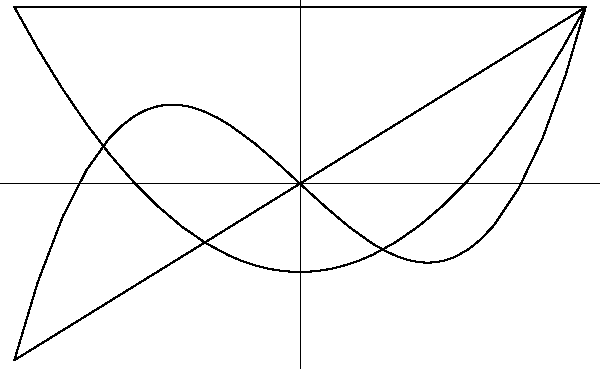
\includegraphics[width=0.4\textwidth]{ode/series/legendre_poly}
      \end{center}
      \caption{The first four Legendre polynomials.}
      \label{fig_legendre_poly}
    \end{figure}
  \item 
    We note that the first two terms in the Legendre equation form an exact 
    derivative.  Thus the Legendre equation can also be written as
    \[ 
    \left( (1 - x^2) y' \right)' = - \alpha (\alpha + 1) y.
    \]
    $P_n$ and $P_m$ are solutions of the Legendre equation.
    \begin{equation}
      \label{eqn legendre pn pm}
      \left( (1 - x^2) P_n' \right)'  = - n (n + 1) P_n, \quad
      \left( (1 - x^2) P_m' \right)'  = - m (m + 1) P_m
    \end{equation}
    We multiply the first relation of Equation~\ref{eqn legendre pn pm}
    by $P_m$ and integrate by parts.
    \begin{gather*}
      \left( (1 - x^2) P_n' \right)' P_m = - n (n + 1) P_n P_m
      \\
      \int_{-1}^1 \left( (1 - x^2) P_n' \right)' P_m \,\dd x 
      = - n (n + 1) \int_{-1}^1 P_n P_m \,\dd x
      \\
      \left[ \left( (1 - x^2) P_n' \right) P_m \right]_{-1}^1 
      - \int_{-1}^1(1 - x^2) P_n' P_m' \,\dd x 
      = - n (n + 1) \int_{-1}^1 P_n P_m \,\dd x
      \\
      \int_{-1}^1 (1 - x^2) P_n' P_m' \,\dd x = n (n + 1) \int_{-1}^1 P_n P_m \,\dd x
    \end{gather*}
    We multiply the secord relation of Equation~\ref{eqn legendre pn pm}
    by $P_n$ and integrate by parts.  To obtain a different expression for
    $\int_{-1}^1 (1 - x^2) P_m' P_n' \,\dd x$.
    \[
    \int_{-1}^1 (1 - x^2) P_m' P_n' \,\dd x = m (m + 1) \int_{-1}^1 P_m P_n \,\dd x 
    \]
    We equate the two expressions for $\int_{-1}^1 (1 - x^2) P_m' P_n' \,\dd x$.
    to obtain an orthogonality relation.
    \begin{gather*}
      (n (n + 1) - m (m + 1)) \int_{-1}^1 P_n P_m \,\dd x = 0 
      \\
      \boxed{
        \int_{-1}^1 P_n(x) P_m(x) \,\dd x = 0\ \mathrm{if}\ n \neq m.
        }
    \end{gather*}
    We verify that for the first four polynomials the value of 
    the integral is $2/(2 n + 1)$ for $n = m$.
    \begin{gather*}
      \int_{-1}^1 P_0(x) P_0(x) \,\dd x = \int_{-1}^1 1 \,\dd x = 2 
      \\
      \int_{-1}^1 P_1(x) P_1(x) \,\dd x = \int_{-1}^1 x^2 \,\dd x 
      = \left[ \frac{x^3}{3} \right]_{-1}^1 = \frac{2}{3}
      \\
      \int_{-1}^1 P_2(x) P_2(x) \,\dd x 
      = \int_{-1}^1 \frac{1}{4} \left( 9 x^4 - 6 x^2 + 1 \right) \,\dd x 
      = \left[ \frac{1}{4} \left( \frac{9 x^5}{5} - 2 x^3 + x \right) \right]_{-1}^1 
      = \frac{2}{5}
      \\
      \int_{-1}^1 P_3(x) P_3(x) \,\dd x 
      = \int_{-1}^1 \frac{1}{4} \left( 25 x^6 - 30 x^4 + 9 x^2 \right) \,\dd x 
      = \left[ \frac{1}{4} \left( \frac{25 x^7}{7} - 6 x^5 + 3 x^3 \right) 
      \right]_{-1}^1 
      = \frac{2}{7}
    \end{gather*}
  \end{enumerate}
\end{Solution}












%%111111111111111111111111111111111111111111111111111111111111111111111111111
\begin{Solution} 
  \label{solution w1sinzw1zz2w=0}
  The indicial equation for this problem is
  \[ \alpha^2 + 1 = 0.\]
  Since the two roots $\alpha_1 = i$ and $\alpha_2 = -i$ are distinct and
  do not differ by an integer, there are two solutions in the Frobenius form.
  \[ w_1 = z^i \sum_{n=0}^\infty a_n z^n, \qquad
  w_1 = z^{-i} \sum_{n=0}^\infty b_n z^n\]
  However, these series are not real-valued on the positive real axis.  
  Recalling that
  \[ z^i = \e^{i \log z} = \cos(\log z) + i\,\sin(\log z), \quad \mathrm{and}\quad
  z^{-i} = \e^{-i \log z} = \cos(\log z) - i\,\sin(\log z),\]
  we can write a new set of solutions that are real-valued on the 
  positive real axis as linear combinations of $w_1$ and $w_2$.
  \[ u_1 = \frac{1}{2}(w_1 + w_2),  \qquad u_2 = \frac{1}{2i}(w_1 - w_2) \]
  \[ \boxed{ u_1 = \cos(\log z) \sum_{n=0}^\infty c_n z^n , \qquad
    u_1 = \sin(\log z) \sum_{n=0}^\infty d_n z^n  }\]
\end{Solution}









%%222222222222222222222222222222222222222222222222222222222222222222222222222
\begin{Solution}
  \label{solution wwz12w=0}
  Consider the equation $w'' + w'/(z-1) + 2w = 0$.

  We see that there is a regular singular point at $z=1$.  All other finite
  values of $z$ are ordinary points of the equation.  To examine the point at
  infinity we introduce the transformation $z = 1/t$, $w(z) = u(t)$.  Writing
  the derivatives with respect to $z$ in terms of $t$ yields
  \[      \frac{d}{dz} = -t^2 \frac{d}{dt},\ \ \ \
  \frac{d^2}{dz^2} = t^4 \frac{d^2}{dt^2} + 2t^3 \frac{d}{dt}. \]
  Substituting into the differential equation gives us
  \begin{align*}
    t^4 u'' + 2t^3 u' - \frac{t^2 u'}{1/t-1} + 2u &= 0 \\
    u'' + \left(\frac{2}{t} - \frac{1}{t(1-t)}\right)u'
    + \frac{2}{t^4} u &= 0.
  \end{align*}
  Since $t = 0$ is an irregular singular point in the equation for $u(t)$,
  $z = \infty$ is an irregular singular point in the equation for $w(z)$.
\end{Solution}













%%333333333333333333333333333333333333333333333333333333333333333333333333333
\begin{Solution}
  \label{solution w54zwz18zw=0}
  Find the series expansions about $z = 0$ for
  \[      w'' + \frac{5}{4z} w' + \frac{z-1}{8z^2} w = 0. \]
  We see that $z=0$ is a regular singular point of the equation.
  The indicial equation is
  \begin{gather*}
    \alpha^2 + \frac{1}{4}\alpha - \frac{1}{8} = 0 \\
    \left( \alpha + \frac{1}{2} \right) \left( \alpha - \frac{1}{4} \right) = 0.
  \end{gather*}
  Since the roots are distinct and do not differ by an integer, there will
  be two solutions in the Frobenius form.
  \[ w_1 = z^{1/4} \sum_{n=0}^\infty a_n(\alpha_1) z^n, \qquad
  w_2 = z^{-1/2} \sum_{n=0}^\infty a_n(\alpha_2) z^n \]

  We multiply the differential equation by $8z^2$ to put it in a better form.
  Substituting a Frobenius series into the differential equation,
  \begin{gather*}
    8z^2 \sum_{n=0}^\infty (n + \alpha)(n + \alpha - 1) a_n z^{n+\alpha-2}
    + 10 z \sum_{n=0}^\infty (n + \alpha) a_n z^{n + \alpha - 1}
    + (z-1) \sum_{n=0}^\infty a_n z^{n + \alpha} \\
    8 \sum_{n=0}^\infty (n + \alpha)(n + \alpha - 1) a_n z^n
    + 10 \sum_{n=0}^\infty (n + \alpha) a_n z^n
    + \sum_{n=1}^\infty a_{n-1} z^n -  \sum_{n=0}^\infty a_n z^n .
  \end{gather*}
  Equating coefficients of powers of $z$,
  \begin{gather*}
    \left[8 (n + \alpha)(n + \alpha - 1) + 10 (n + \alpha)
      - 1 \right] a_n = - a_{n-1} \\
    a_n = - \frac{a_{n-1}}{8(n+\alpha)^2 + 2 (n+\alpha)-1}.
  \end{gather*}

  \paragraph{The First Solution.}
  Setting $\alpha = 1/4$ in the recurrence formula,
  \begin{align*}
    a_n(\alpha_1)   &= -\frac{a_{n-1}}{8(n + 1/4)^2 + 2 (n + 1/4) - 1} \\
    a_n(\alpha_1)   &= -\frac{a_{n-1}}{2n(4n+3)} .
  \end{align*}
  Thus the first solution is
  \[ \boxed{ w_1 = z^{1/4} \sum_{n=0}^\infty a_n(\alpha_1) z^n
    = a_0 z^{1/4} \left( 1 - \frac{1}{14} z + \frac{1}{616} z^2 + \cdots
    \right).} \]

  \paragraph{The Second Solution.}
  Setting $\alpha = -1/2$ in the recurrence formula,
  \begin{align*}
    a_n &= - \frac{a_{n-1}}{8(n-1/2)^2 + 2 (n-1/2)-1} \\
    a_n &= - \frac{a_{n-1}}{2n(4n-3)} 
  \end{align*}
  Thus the second linearly independent solution is
  \[ \boxed{ w_2 = z^{-1/2} \sum_{n=0}^\infty a_n(\alpha_2) z^n
    = a_0 z^{-1/2} \left(1 - \frac{1}{2}z + \frac{1}{40}z^2 
      + \cdots \right) .} \]
\end{Solution}









%%444444444444444444444444444444444444444444444444444444444444444444444444444444
\begin{Solution}
  \label{solution wzww=0}
  We consider the series solutions of,
  \[ 
  w'' + z w' + w = 0. 
  \]
  We would like to find the expansions of the fundamental set of solutions
  about $z = 0$.  Since $z = 0$ is a regular point, (the coefficient functions
  are analytic there), we expand the solutions in Taylor series.
  Differentiating the series expansions for $w(z)$,
  \begin{align*}
    w       &= \sum_{n=0}^\infty a_n z^n \\
    w'      &= \sum_{n=1}^\infty n a_n z^{n-1} \\
    w''     &= \sum_{n=2}^\infty n(n-1)a_n z^{n-2} \\
    &= \sum_{n=0}^\infty (n+2)(n+1) a_{n+2} z^n
  \end{align*}
  We may take the lower limit of summation to be zero without changing 
  the sums.  Substituting these expressions into the differential equation,
  \begin{gather*}
    \sum_{n=0}^\infty (n+2)(n+1) a_{n+2} z^n + \sum_{n=0}^\infty n a_n z^{n}
    + \sum_{n=0}^\infty a_n z^n = 0 \\
    \sum_{n=0}^\infty \big( (n+2)(n+1) a_{n+2} + (n+1)a_n \big) z^n = 0 .
  \end{gather*}
  Equating the coefficient of the $z^n$ term gives us
  \begin{gather*}
    (n+2)(n+1) a_{n+2} + (n+1)a_n = 0 , \qquad n \geq 0 \\
    a_{n+2} = -\frac{a_n}{n+2}, \qquad n \geq 0.
  \end{gather*}
  $a_0$ and $a_1$ are arbitrary. 
  We determine the rest of the coefficients from the recurrence relation.
  We consider the cases for even and odd $n$ separately.
  \begin{align*}
    a_{2n}  &= -\frac{a_{2n-2}}{2n} \\
    &= \frac{a_{2n-4}}{(2n)(2n-2)} \\
    &= (-1)^n \frac{a_0}{(2n)(2n-2) \cdots 4 \cdot 2} \\
    &= (-1)^n \frac{a_0}{ \prod_{m=1}^n 2m }, \quad n \geq 0 
  \end{align*}
  \begin{align*}
    a_{2n+1} &= -\frac{a_{2n-1}}{2n+1} \\
    &= \frac{a_{2n-3}}{(2n+1)(2n-1)} \\
    &= (-1)^n \frac{a_1}{(2n+1)(2n-1)\cdots 5 \cdot 3 } \\
    &= (-1)^n \frac{a_1}{ \prod_{m=1}^n (2m+1) }, \quad n \geq 0 
  \end{align*}
  If $\{w_1, w_2\}$ is the fundamental set of solutions, then the initial
  conditions demand that
  $w_1 = 1 + 0 \cdot z + \cdots$ and $w_2 = 0 + z + \cdots$.  We see that
  $w_1$ will have only even powers of $z$ and $w_2$ will have only odd powers
  of $z$.
  \[ 
  \boxed{ 
    w_1 = \sum_{n=0}^\infty \frac{ (-1)^n }{ \prod_{m=1}^n 2 m } z^{2 n},
    \qquad
    w_2 = \sum_{n=0}^\infty \frac{ (-1)^n }{ \prod_{m=1}^n (2 m + 1) } z^{2 n + 1}
    }
  \]
  Since the coefficient functions in the differential equation are entire, 
  (analytic in the finite complex plane), the radius of convergence of 
  these series solutions is infinite.
\end{Solution}











%%555555555555555555555555555555555555555555555555555555555555555555555555555555
\begin{Solution}
  \label{solution w12zw1zw=0}
  \[ w'' + \frac{1}{2z} w' + \frac{1}{z} w = 0. \]
  We can find the indicial equation by substituting
  $w = z^\alpha + \mathcal{O}(z^{\alpha+1})$ into the differential equation.
  \begin{gather*}
    \alpha(\alpha-1) z^{\alpha-2} + \frac{1}{2} \alpha z^{\alpha-2}
    + z^{\alpha-1} = \mathcal{O}(z^{\alpha-1}) \\
    \intertext{Equating the coefficient of the $z^{\alpha-2}$ term,}
    \alpha(\alpha-1) + \frac{1}{2} \alpha = 0 \\
    \alpha = 0, \frac{1}{2}.
  \end{gather*}
  Since the roots are distinct and do not differ by an integer, the solutions
  are of the form
  \[ w_1 = \sum_{n=0}^\infty a_n z^n, \qquad w_2 = z^{1/2} \sum_{n=0}^\infty b_n z^n. \]

  Differentiating the series for the first solution,
  \begin{align*}
    w_1     &= \sum_{n=0}^\infty a_n z^n \\
    w_1'    &= \sum_{n=1}^\infty n a_n z^{n-1} \\
    &= \sum_{n=0}^\infty (n+1) a_{n+1} z^n \\
    w_1''   &= \sum_{n=1}^\infty n (n+1) a_{n+1} z^{n-1}.
  \end{align*}
  Substituting this series into the differential equation,
  \[
  \sum_{n=1}^\infty n (n+1) a_{n+1} z^{n-1}
  + \frac{1}{2 z} \sum_{n=0}^\infty (n+1) a_{n+1} z^n
  + \frac{1}{z} \sum_{n=0}^\infty a_n z^n  = 0
  \]
  \[
  \sum_{n=1}^\infty \left[ n(n+1) a_{n+1} + \frac{1}{2} (n+1) a_{n+1} + a_n \right]
  z^{n-1} + \frac{1}{2 z} a_1 + \frac{1}{z} a_0 = 0.
  \]
  Equating powers of $z$,
  \begin{alignat*}{2}
    &z^{-1}: \frac{a_1}{2} + a_0 = 0 \quad &\to \quad
    &a_1 = - 2 a_0 \\
    &z^{n-1}: \left(n+\frac{1}{2}\right) (n+1) a_{n+1} + a_n = 0 \quad &\to \quad
    &a_{n+1} = - \frac{a_n}{(n+1/2)(n+1)}.
  \end{alignat*}
  We can combine the above two equations for $a_n$.
  \[
  a_{n+1} = - \frac{a_n}{(n+1/2)(n+1)}, \quad \mathrm{for}\ n \geq 0
  \]
  Solving this difference equation for $a_n$,
  \[
  a_n = a_0 \prod_{j=0}^{n-1} \frac{-1}{(j+1/2)(j+1)}
  \]
  \[
  \boxed{
    a_n = a_0 \frac{(-1)^n}{n!} \prod_{j=0}^{n-1} \frac{1}{j+1/2}
    }
  \]

  Now let's find the second solution.  Differentiating $w_2$,
  \begin{align*}
    w_2' &= \sum_{n=0}^\infty (n+1/2) b_n z^{n-1/2} \\
    w_2'' &= \sum_{n=0}^\infty (n+1/2)(n-1/2) b_n z^{n-3/2}.
  \end{align*}
  Substituting these expansions into the differential equation,
  \[ \sum_{n=0}^\infty (n+1/2)(n-1/2) b_n z^{n-3/2} + \frac{1}{2} \sum_{n=0}^\infty (n+1/2)b_n
  z^{n-3/2} + \sum_{n=1}^\infty b_{n-1} z^{n-3/2} = 0.\]
  Equating the coefficient of the $z^{-3/2}$ term,
  \[ \frac{1}{2} \left(-\frac{1}{2} \right) b_0 + \frac{1}{2}\frac{1}{2} b_0
  = 0, \]
  we see that $b_0$ is arbitrary.  Equating the other coefficients of powers of
  $z$,
  \begin{gather*}
    (n+1/2)(n-1/2) b_n + \frac{1}{2} (n+1/2)b_n + b_{n-1} = 0 \\
    b_n = - \frac{b_{n-1}}{n(n+1/2)}
  \end{gather*}
  Calculating the $b_n$'s,
  \begin{align*}
    b_1     &= - \frac{b_0}{1\cdot \frac{3}{2}} \\
    b_2     &= \frac{b_0}{1\cdot 2 \cdot \frac{3}{2} \cdot \frac{5}{2}} \\
    b_n     &= \frac{(-1)^n 2^n b_0}{n! \cdot 3 \cdot 5 \cdots (2n+1)}
  \end{align*}
  Thus the second solution is
  \[ \boxed{w_2 = b_0 z^{1/2} \sum_{n=0}^\infty \frac{(-1)^n 2^n z^n}
    {n!\ 3 \cdot 5 \cdots (2n+1)}.} \]
\end{Solution}








%%666666666666666666666666666666666666666666666666666666666666666666666666666666
\begin{Solution}
  \label{solution w2z3zw1zw=0}
  \[ w'' + \left(\frac{2}{z}+ \frac{3}{z^2} \right)w' + \frac{1}{z^2} w = 0. \]
  In order to analyze the behavior at infinity we make the change of
  variables $t = 1/z$, $u(t) = w(z)$ and examine the point $t = 0$.
  Writing the derivatives with respect to $z$ in terms if $t$ yields
  \begin{align*}
    z       &= \frac{1}{t} \\
    d z      &= -\frac{1}{t^2} d t \\
    \frac{\dd}{\dd z}    &= - t^2 \frac{\dd}{\dd t}
  \end{align*}
  \begin{align*}
    \frac{\dd^2}{\dd z^2}    &= -t^2 \frac{\dd}{\dd t} \left( - t^2 \frac{\dd}{\dd t} \right) \\
    &= t^4 \frac{\dd^2}{\dd t^2} + 2 t^3 \frac{\dd}{\dd t}.
  \end{align*}
  The equation for $u$ is then
  \begin{gather*}
    t^4 u'' + 2 t^3 u' + (2t + 3 t^2)(-t^2)u' + t^2 u = 0 \\
    u'' + -3 u' + \frac{1}{t^2} u = 0
  \end{gather*}
  We see that $t=0$ is a regular singular point.  To find the indicial
  equation, we substitute $u = t^\alpha + \mathcal{O}(t^{\alpha+1})$ 
  into the differential
  equation.
  \begin{gather*}
    \alpha(\alpha-1)t^{\alpha-2} - 3 \alpha t^{\alpha-1} + t^{\alpha-2} =
    \mathcal{O}(t^{\alpha-1}) \\
    \intertext{Equating the coefficients of the $t^{\alpha-2}$ terms,}
    \alpha(\alpha-1) + 1 = 0 \\
    \alpha = \frac{1 \pm i \sqrt{3}}{2}
  \end{gather*}
  Since the roots of the indicial equation are distinct and do not differ by
  an integer, a set of solutions has the form
  \[ \left\{ t^{(1+i\sqrt{3})/2} \sum_{n=0}^\infty a_n t^n, \quad
    t^{(1-i\sqrt{3})/2} \sum_{n=0}^\infty b_n t^n \right\}. \]
  Noting that
  \[ t^{(1+i\sqrt{3})/2} = t^{1/2} \exp\left(\frac{i\sqrt{3}}{2} \log t\right),
  \quad \mathrm{and} \quad
  t^{(1-i\sqrt{3})/2} = t^{1/2} \exp\left(-\frac{i\sqrt{3}}{2} \log t\right). \]
  We can take the sum and difference of the above solutions to obtain the
  form
  \[ u_1 = t^{1/2} \cos\left( \frac{\sqrt{3}}{2} \log t \right)
  \sum_{n=0}^\infty a_n t^n,
  \qquad
  u_1 = t^{1/2} \sin\left( \frac{\sqrt{3}}{2} \log t \right)
  \sum_{n=0}^\infty b_n t^n. \]
  Putting the answer in terms of $z$, we have the form of the two Frobenius
  expansions about infinity.
  \[ \boxed{ w_1 = z^{-1/2} \cos\left(\frac{\sqrt{3}}{2} \log z \right)
    \sum_{n=0}^\infty \frac{a_n}{z^n}, \qquad
    w_1 = z^{-1/2} \sin\left(\frac{\sqrt{3}}{2} \log z \right)
    \sum_{n=0}^\infty \frac{b_n}{z^n}. } \]
\end{Solution}






%% x \frac{\dd^2 y}{\dd x^2} + (b - x) \frac{\dd y}{\dd x} - a y = 0
\begin{Solution}
  \label{solution xybxyay=0}
  \begin{enumerate}
    %%
    %%
  \item
    We write the equation in the standard form.
    \[
    y'' + \frac{b - x}{x} y' - \frac{a}{x} y = 0
    \]
    Since $\frac{b-x}{x}$ has no worse than a first order pole and $\frac{a}{x}$
    has no worse than a second order pole at $x = 0$, that is a regular 
    singular point.  Since the coefficient functions have no other singularities
    in the finite complex plane, all the other points in the finite complex
    plane are regular points.

    Now to examine the point at infinity.  We make the change of variables
    $u(\xi) = y(x)$, $\xi = 1/x$.
    \begin{gather*}
      y' = \frac{\dd \xi}{\dd x} \frac{\dd}{\dd \xi} u = - \frac{1}{x^2} u' = -\xi^2 u' \\
      y'' = - \xi^2 \frac{\dd}{\dd \xi} \left( -\xi^2 \frac{\dd}{\dd \xi} \right) u
      = \xi^4 u'' + 2 \xi^3 u'
    \end{gather*}
    The differential equation becomes
    \begin{gather*}
      x y'' + (b - x) y' - a y \\
      \frac{1}{\xi} \left( \xi^4 u'' + 2 \xi^3 u' \right) + 
      \left( b - \frac{1}{\xi} \right) \left( - \xi^2 u' \right) - a u = 0 \\
      \xi^3 u'' + \left( (2 - b) \xi^2 + \xi \right) u' - a u = 0 \\
      u'' + \left( \frac{2-b}{\xi} + \frac{1}{\xi^2} \right) - \frac{a}{\xi^3} u = 0
    \end{gather*}
    Since this equation has an irregular singular point at $\xi = 0$, the equation
    for $y(x)$ has an irregular singular point at infinity.
    %%
    %%
  \item
    The coefficient functions are
    \begin{gather*}
      p(x) \equiv \frac{1}{x} \sum_{n=1}^\infty p_n x^n = \frac{1}{x} (b - x), \\
      q(x) \equiv \frac{1}{x^2} \sum_{n=1}^\infty q_n x^n = \frac{1}{x^2} (0 - a x).
    \end{gather*}
    The indicial equation is
    \begin{gather*}
      \alpha^2 + (p_0 - 1) \alpha + q_0 = 0 \\
      \alpha^2 + (b - 1) \alpha + 0 = 0 \\
      \boxed{
        \alpha( \alpha + b - 1 ) = 0.
        }
    \end{gather*}
    %%
    %%
  \item
    Since one of the roots of the indicial equation is zero, and the other 
    root is not a negative integer, one of the solutions of the differential
    equation is a Taylor series.  
    \begin{align*}
      y_1 &= \sum_{k=0}^\infty c_k x^k \\
      y_1' &= \sum_{k=1}^\infty k c_k x^{k-1} \\
      &= \sum_{k=0}^\infty (k+1) c_{k+1} x^k \\
      &= \sum_{k=0}^\infty k c_k x^{k-1} \\
      y_1'' &= \sum_{k = 2} k(k-1) c_k x^{k-2} \\
      &= \sum_{k=1}^\infty (k+1)k c_{k+1} x^{k-1} \\
      &= \sum_{k=0}^\infty (k+1)k c_{k+1} x^{k-1} 
    \end{align*}
    We substitute the Taylor series into the differential equation.
    \begin{gather*}
      x y'' + (b - x) y' - a y = 0 \\
      \sum_{k=0}^\infty (k+1)k c_{k+1} x^k + b \sum_{k=0}^\infty (k+1) c_{k+1} x^k
      - \sum_{k=0}^\infty k c_k x^k - a\sum_{k=0}^\infty c_k x^k = 0 
    \end{gather*}
    We equate coefficients to determine a recurrence relation for the coefficients.
    \begin{gather*}
      (k+1) k c_{k+1} + b (k+1) c_{k+1} - k c_k - a c_k = 0 \\
      c_{k+1} = \frac{k + a}{(k+1)(k+b)} c_k 
    \end{gather*}
    For $c_0 = 1$, the recurrence relation has the solution
    \[
    c_k = \frac{ (a)_k x^k }{ (b)_k k! }.
    \]
    Thus one solution is
    \[
    \boxed{
      y_1(x) =  \sum_{k=0}^\infty \frac{ (a)_k }{ (b)_k k! } x^k.
      }
    \]
    %%
    %%
  \item
    If $a = -m$, where $m$ is a non-negative integer, then $(a)_{k} = 0$
    for $k > m$.  This makes $y_1$ a polynomial:
    \[
    \boxed{
      y_1(x) =  \sum_{k=0}^m \frac{ (a)_k }{ (b)_k k! } x^k.
      }
    \]
    %%
    %%
  \item
    If $b = n+1$, where $n$ is a non-negative integer, the indicial equation is
    \[
    \alpha( \alpha + n ) = 0.
    \]
    For the case $n = 0$, the indicial equation has a double root at zero.  
    Thus the solutions have the form:
    \[
    \boxed{
      y_1(x) =  \sum_{k=0}^m \frac{ (a)_k }{ (b)_k k! } x^k, \qquad
      y_2(x) = y_1(x) \log x + \sum_{k=0}^\infty d_k x^k
      }
    \]
    For the case $n > 0$ the roots of the indicial equation differ by an
    integer.  The solutions have the form:
    \[
    \boxed{
      y_1(x) =  \sum_{k=0}^m \frac{ (a)_k }{ (b)_k k! } x^k, \qquad
      y_2(x) = d_{-1} y_1(x) \log x + x^{-n} \sum_{k=0}^\infty d_k x^k
      }
    \]
    The form of the solution for $y_2$ can be substituted into the equation 
    to determine the coefficients $d_k$.
  \end{enumerate}
\end{Solution}













\begin{Solution}
  \label{solution xy+2xy+6exy=0}
  We write the equation in the standard form.
  \begin{gather*}
    x y'' + 2 x y' + 6 \e^x y = 0
    \\
    y'' + 2 y' + 6 \frac{\e^x}{x} y = 0
  \end{gather*}
  We see that $x = 0$ is a regular singular point.
  The indicial equation is 
  \begin{gather*}
    \alpha^2 - \alpha = 0
    \\
    \alpha = 0,1.
  \end{gather*}
  The first solution has the Frobenius form.
  \[
  y_1 = x + a_2 x^2 + a_3 x^3 + \mathcal{O}(x^4)
  \]
  We substitute $y_1$ into the differential equation and equate coefficients
  of powers of $x$.
  \[
  x y'' + 2 x y' + 6 \e^x y = 0
  \]
  \begin{multline*}
    x ( 2 a_2 + 6 a_3 x + \mathcal{O}(x^2) )
    + 2 x ( 1 + 2 a_2 x + 3 a_3 x^2 + \mathcal{O}(x^3) )
    \\
    + 6 ( 1 + x + x^2/2 + \mathcal{O}(x^3) )( x + a_2 x^2 + a_3 x^3 + \mathcal{O}(x^4) )
    = 0
  \end{multline*}
  \begin{gather*}
    ( 2 a_2 x + 6 a_3 x^2 )
    + ( 2 x + 4 a_2 x^2 )
    + ( 6 x + 6(1 + a_2) x^2 ) = \mathcal{O}(x^3)
    = 0
    \\
    a_2 = -4, \quad a_3 = \frac{17}{3}
    \\
    \boxed{
      y_1 = x -4 x^2 + \frac{17}{3} x^3 + \mathcal{O}(x^4)
      }
  \end{gather*}
  Now we see if the second solution has the Frobenius form.
  There is no $a_1 x$ term because $y_2$ is only determined up to an additive 
  constant times $y_1$.  
  \[
  y_2 = 1 + \mathcal{O}(x^2)
  \]
  We substitute $y_2$ into the differential equation and equate coefficients
  of powers of $x$.
  \begin{gather*}
    x y'' + 2 x y' + 6 \e^x y = 0
    \\
    \mathcal{O}(x) + \mathcal{O}(x) 
    + 6 ( 1 + \mathcal{O}(x) )( 1 + \mathcal{O}(x^2) ) = 0
    \\
    6 = \mathcal{O}(x)
  \end{gather*}
  The substitution $y_2 = 1 + \mathcal{O}(x)$ has yielded a contradiction.
  Since the second solution is not of the Frobenius form, it has the 
  following form:
  \[
  y_2 = y_1 \ln(x) + a_0 + a_2 x^2 + \mathcal{O}(x^3)
  \]
  The first three terms in the solution are
  \[
  y_2 = a_0 + x \ln x - 4 x^2 \ln x + \mathcal{O}(x^2).
  \]
  We calculate the derivatives of $y_2$.
  \begin{align*}
    y_2' &= \ln(x) + \mathcal{O}(1) 
    \\
    y_2'' &= \frac{1}{x} + \mathcal{O}(\ln(x))
  \end{align*}
  We substitute $y_2$ into the differential equation and equate coefficients.
  \begin{gather*}
    x y'' + 2 x y' + 6 \e^x y = 0
    \\
    \left( 1 + \mathcal{O}(x \ln x) \right)
    + 2 \left( \mathcal{O}(x \ln x) \right)
    + 6 \left( a_0 + \mathcal{O}(x \ln x) \right) = 0
    \\
    1 + 6 a_0 = 0
    \\
    \boxed{
      y_2 = - \frac{1}{6} + x \ln x - 4 x^2 \ln x + \mathcal{O}(x^2)
      }
  \end{gather*}
\end{Solution}







}


\raggedbottom
%%=============================================================================
\pagebreak
\flushbottom
\section{Quiz}


\begin{QuizProblem}
  \label{quiz problem definition convergence series}
  Write the definition of convergence of the series $\sum_{n=1}^\infty a_n$.

  \quizsolution{definition convergence series}
\end{QuizProblem}


\begin{QuizProblem}
  \label{quiz problem Cauchy convergence series}
  What is the Cauchy convergence criterion for series?

  \quizsolution{Cauchy convergence series}
\end{QuizProblem}


\begin{QuizProblem}
  \label{quiz problem absolute uniform convergence}
  Define absolute convergence and uniform convergence.  What is the 
  relationship between the two?

  \quizsolution{absolute uniform convergence}
\end{QuizProblem}


\begin{QuizProblem}
  \label{quiz problem geometric series}
  Write the geometric series and the function to which it converges.  
  For what values of the variable does the series converge?

  \quizsolution{geometric series}
\end{QuizProblem}


\begin{QuizProblem}
  \label{quiz problem convergence na}
  For what real values of $a$ does the series $\sum_{n=1}^\infty n^a$ converge?

  \quizsolution{convergence na}
\end{QuizProblem}


\begin{QuizProblem}
  \label{quiz problem ratio root convergence}
  State the ratio and root convergence tests.

  \quizsolution{ratio root convergence}
\end{QuizProblem}


\begin{QuizProblem}
  \label{quiz problem integral convergence test}
  State the integral convergence test.

  \quizsolution{integral convergence test}
\end{QuizProblem}







\raggedbottom
%%=============================================================================
\pagebreak
\flushbottom
\section{Quiz Solutions}


\begin{QuizSolution}
  \label{quiz solution definition convergence series}
  The series $\sum_{n=1}^\infty a_n$ converges if the sequence of partial sums,
  $S_N = \sum_{n=1}^{N} a_n$,
  converges.  That is,
  \[
  \lim_{N \to \infty} S_N =
  \lim_{N \to \infty} \sum_{n=1}^N a_n = \mathrm{constant}.
  \]
\end{QuizSolution}


\begin{QuizSolution}
  \label{quiz solution Cauchy convergence series}
  A series converges if and only if for any $\epsilon > 0$ there
  exists an $N$ such that $|S_n - S_m| < \epsilon$ for all $n,m > N$.
\end{QuizSolution}


\begin{QuizSolution}
  \label{quiz solution absolute uniform convergence}
  The series $\sum_{n=1}^\infty a_n$ converges absolutely if $\sum_{n=1}^\infty |a_n|$
  converges.
  If the rate of convergence of $\sum_{n=1}^\infty a_n(z)$ is independent of $z$ then 
  the series is uniformly convergent.  
  The series is uniformly convergent in a domain if for any given 
  $\epsilon > 0$ there exists an $N$, independent of $z$, such that
  \[
  |f(z) - S_{N}(z)|
  = \left|f(z) - \sum_{n=1}^{N} a_n(z) \right| < \epsilon
  \]
  for all $z$ in the domain.

  There is no relationship between absolute convergence and 
  uniform convergence.
\end{QuizSolution}


\begin{QuizSolution}
  \label{quiz solution geometric series}
  \[
  \frac{1}{1-z} = \sum_{n=0}^\infty z^n \quad \mathrm{for}\ |z| < 1.
  \]
\end{QuizSolution}


\begin{QuizSolution}
  \label{quiz solution convergence na}
  The series converges for $a < -1$.
\end{QuizSolution}


\begin{QuizSolution}
  \label{quiz solution ratio root convergence}
  The series $\sum_{n=1}^\infty a_n$ converges absolutely if
  \[
  \lim_{n \to \infty} \left| \frac{a_{n+1}}{a_n} \right| < 1.
  \]
  If the limit is greater than unity, then the series diverges.  If the
  limit is unity, the test fails.

  The series $\sum_{n=1}^\infty a_n$ converges absolutely if
  \[
  \lim_{n \to \infty} |a_n|^{1/n} < 1.
  \]
  If the limit is greater than unity, then the series diverges.  If the
  limit is unity, the test fails.
\end{QuizSolution}


\begin{QuizSolution}
  \label{quiz solution integral convergence test}
  If the coefficients $a_n$ of a series $\sum_{n=1}^\infty a_n$
  are monotonically decreasing and
  can be extended to a monotonically decreasing function of the continuous
  variable $x$:
  \[
  a(x) = a_n \quad \mathrm{for integer}\ x,
  \]
  then the sum converges or diverges with the integral:
  \[
  \int_1^\infty a(x) \,\dd x.
  \]
\end{QuizSolution}






\raggedbottom


\flushbottom


%%=============================================================================
%%=============================================================================
\chapter{Asymptotic Expansions}
\index{asymptotic expansions}


The more you sweat in practice, the less you bleed in battle.

\begin{flushright}
  -Navy Seal Saying
\end{flushright}

%%=============================================================================
\section{Asymptotic Relations}
\index{asymptotic relations}



\paragraph{The $\boldsymbol{\ll}$ and $\boldsymbol{\sim}$ symbols.}
First we will introduce two new symbols used in asymptotic relations.
\[ f(x) \ll g(x)\quad\mathrm{as}\ x \to x_0,\]
is read, ``$f(x)$ is much smaller than $g(x)$ as $x$ tends to $x_0$''.  
This means
\[\lim_{x \to x_0} \frac{f(x)}{g(x)} = 0.\]
The notation
\[ f(x) \sim g(x)\quad \mathrm{as}\ x \to x_0, \]
is read ``$f(x)$ is asymptotic to $g(x)$ as $x$ tends to $x_0$'';  which means
\[ \lim_{x \to x_0} \frac{f(x)}{g(x)} = 1.\]
A few simple examples are
\begin{itemize}
\item $-\e^x \gg x \quad \mathrm{as}\ x \to +\infty$
\item $\sin x \sim x \quad \mathrm{as}\ x \to 0$ 
\item $1/x \ll 1 \quad \mathrm{as}\ x \to +\infty$
\item $\e^{-1/x} \ll x^{-n} \quad \mathrm{as}\ x \to 0^+\ \mathrm{for all}\ n$
\end{itemize}


An equivalent definition of $f(x) \sim g(x)$ as $x \to x_0$ is
\[ f(x) - g(x) \ll g(x) \quad \mathrm{as}\ x \to x_0.\]
Note that it does not make sense to say that a function $f(x)$ 
is asymptotic to zero.  Using the above definition this would imply
\[ f(x) \ll 0 \quad \mathrm{as}\ x \to x_0.\]
If you encounter an expression like
$f(x) + g(x) \sim 0$, take this to mean $f(x) \sim - g(x)$.





\paragraph{The Big $\mathbf{\mathcal{O}}$ and Little $\mathbf{\mathsf{o}}$ 
  Notation.}
If $|f(x)| \leq m |g(x)|$ for some constant $m$ in some 
neighborhood of the point $x = x_0$, then we say that
\[ f(x) = \mathcal{O}(g(x)) \quad \mathrm{as}\ x \to x_0.\]
We read this as ``$f$ is big $\mathcal{O}$ of $g$ as $x$ goes to $x_0$''.
If $g(x)$ does not vanish, an equivalent definition is that
$f(x) / g(x)$ is bounded as $x \to x_0$.

If for any given positive $\delta$ there exists a neighborhood of $x=x_0$
in which $|f(x)| \leq \delta |g(x)|$ then 
\[ f(x) = \mathsf{o}(g(x)) \quad \mathrm{as}\ x \to x_0.\]
This is read, ``$f$ is little $o$ of $g$ as $x$ goes to $x_0$.''

For a few examples of the use of this notation,
\begin{itemize}
\item $ \e^{-x} = \mathsf{o}(x^{-n})$ as $x \to \infty$ for any $n$. 
\item $\sin x = \mathcal{O}(x)$ as $x \to 0$.
\item $\cos x - 1 = \mathsf{o}(1)$ as $x \to 0$.
\item $\log x = \mathsf{o}(x^\alpha)$ as $x \to +\infty$ 
  for any positive $\alpha$.
\end{itemize}



\paragraph{Operations on Asymptotic Relations.}
You can perform the ordinary arithmetic operations on asymptotic relations.
Addition, multiplication, and division are valid.

You can always integrate an asymptotic relation.  Integration is a smoothing
operation.  However, it is necessary to exercise some care.




\begin{Example}
  Consider 
  \[ f'(x) \sim \frac{1}{x^2} \quad \mathrm{as}\ x \to \infty.\]
  This does not imply that
  \[ f(x) \sim \frac{-1}{x} \quad \mathrm{as}\ x \to \infty.\]
  We have forgotten the constant of integration. Integrating the 
  asymptotic relation for $f'(x)$ yields
  \[ f(x) \sim \frac{-1}{x} + c \quad \mathrm{as}\ x \to \infty. \]
  If $c$ is nonzero then
  \[ f(x) \sim c \quad \mathrm{as}\ x \to \infty. \]
\end{Example}


It is not always valid to differentiate an asymptotic relation.  



\begin{Example}
  Consider $f(x) = \frac{1}{x} + \frac{1}{x^2} \sin(x^3)$.
  \[ f(x) \sim \frac{1}{x} \quad \mathrm{as}\ x \to \infty.\]
  Differentiating this relation yields
  \[f'(x) \sim -\frac{1}{x^2} \quad \mathrm{as}\ x \to \infty.\]
  However, this is not true since
  \begin{align*}
    f'(x)   &= -\frac{1}{x^2} - \frac{2}{x^3}\sin(x^3) + 2 \cos(x^3) \\
    &\not\sim -\frac{1}{x^2} \quad \mathrm{as}\ x \to \infty.
  \end{align*}
\end{Example}




\paragraph{The Controlling Factor.}
The controlling factor is the most rapidly varying factor in an asymptotic
relation.  Consider a function $f(x)$ that is asymptotic to $x^2 \e^x$
as $x$ goes to infinity.  The controlling factor is $\e^x$.  
For a few examples of this,
\begin{itemize}
\item $x \log x$ has the controlling factor $x$ as $x \to \infty$.
\item $x^{-2} \e^{1/x}$ has the controlling factor $\e^{1/x}$ as $x \to 0$.
\item $x^{-1} \sin x$ has the controlling factor $\sin x$ as $x \to \infty$.
\end{itemize}



\paragraph{The Leading Behavior.}
Consider a function that is asymptotic to a sum of terms.  
\[ f(x) \sim a_0(x) + a_1(x) + a_2(x) + \cdots, \quad \mathrm{as}\ x \to x_0.\]
where 
\[ a_0(x) \gg a_1(x) \gg a_2(x) \gg \cdots, \quad \mathrm{as}\ x \to x_0.\]
The first term in the sum is the leading order behavior.  For a few 
examples,
\begin{itemize}
\item For $\sin x \sim x - x^3/6 + x^5 / 120 - \cdots$ as $x \to 0$, the leading
  order behavior is $x$.
\item For $f(x) \sim \e^x(1 - 1/x + 1/x^2 - \cdots)$ as $x \to \infty$, the leading
  order behavior is $\e^x$.
\end{itemize}





%%============================================================================
\section{Leading Order Behavior of Differential Equations}
\index{leading order behavior!for differential equations}

It is often useful to know the leading order behavior of the solutions
to a differential equation.  If we are considering a regular point
or a regular singular point, the approach is straight forward.  We simply
use a Taylor expansion or the Frobenius method.  However, if we are
considering an irregular singular point, we will have to be a little
more creative.  Instead of an all encompassing theory like the
Frobenius method which always gives us the solution, 
we will use a heuristic approach that usually gives us the solution.







\begin{Example}
  Consider the Airy equation
  \[ y'' = x y. \]
  We
  \footnote{Using "We" may be a bit presumptuous on my part. Even if
    you don't particularly want to know how the solutions behave, I urge
    you to just play along.  This is an interesting section, I promise.}
  would like to know how the solutions of this equation behave as
  $x \to + \infty$.
  First we need to classify the point at infinity.  The change of variables
  \[ x = \frac{1}{t}, \quad y(x) = u(t), \quad \frac{\dd}{\dd x} = -t^2\frac{\dd}{\dd t},
  \quad \frac{\dd^2}{\dd x^2} = t^4 \frac{\dd^2}{\dd t^2} + 2t^3 \frac{\dd}{\dd t}\]
  yields
  \begin{gather*}
    t^4 u'' + 2 t^3 u' = \frac{1}{t} u \\
    u'' + \frac{2}{t} u' - \frac{1}{t^5} u = 0.
  \end{gather*}
  Since the equation for $u$ has an irregular singular point at zero, the equation for 
  $y$ has an irregular singular point at infinity.

  \paragraph{The Controlling Factor.}
  Since the solutions at irregular singular points often have exponential behavior, we
  make the substitution $y = \e^{s(x)}$ into the differential equation for $y$.
  \begin{gather*}
    \frac{\dd^2}{\dd x^2} \big[ \e^s \big] = x \e^s \\
    \big[s'' + (s')^2\big] \e^s = x \e^s \\
    s'' + (s')^2 = x
  \end{gather*}

  \paragraph{The Dominant Balance.}
  Now we have a differential equation for $s$ that appears harder to solve than our equation
  for $y$.  However, we did not introduce the substitution in order to obtain an equation 
  that we could solve exactly.  We are looking for an equation that we can solve
  approximately in the limit as $x \to \infty$.  If one of the terms in the equation for
  $s$ is much smaller that the other two as $x \to \infty$, then dropping that term and solving
  the simpler equation may give us an approximate solution.  If one of the terms in the 
  equation for $s$ is much smaller than the others then we say that the remaining
  terms form a \textbf{dominant balance} in the limit as $x \to \infty$.

  Assume that the $s''$ term is much smaller that the others, 
  $s'' \ll (s')^2, x$ as $x \to \infty$.  This gives us
  \begin{gather*}
    (s')^2 \sim x  \\
    s' \sim \pm \sqrt{x} \\
    s \sim \pm \frac{2}{3} x^{3/2} \quad \mathrm{as}\ x \to \infty.
  \end{gather*}
  Now let's check our assumption that the $s''$ term is small.  Assuming that we can 
  differentiate the asymptotic relation $s' \sim \pm \sqrt{x}$, we obtain 
  $s'' \sim \pm \frac{1}{2} x^{-1/2}$ as $x \to \infty$.
  \[ s'' \ll (s')^2, x \qquad \to \qquad x^{-1/2} \ll x \quad \mathrm{as}\ x \to \infty \]
  Thus we see that the behavior we found for $s$ is consistent with our assumption.
  The controlling factors for solutions to the Airy equation are $\exp(\pm \frac{2}{3}
  x^{3/2})$ as $x \to \infty$.

  \paragraph{The Leading Order Behavior of the Decaying Solution.}
  Let's find the leading order behavior as $x$ goes to infinity of the solution with the
  controlling factor $\exp(-\frac{2}{3} x^{3/2})$.  We substitute
  \[ s(x) = -\frac{2}{3} x^{3/2} + t(x), \qquad \mathrm{where}\ t(x) \ll x^{3/2}\ \mathrm{as}\ 
  x \to \infty \]
  into the differential equation for $s$.
  \begin{gather*}
    s'' + (s')^2 = x \\
    -\frac{1}{2} x^{-1/2} + t'' + (-x^{1/2} + t')^2 = x \\
    t'' + (t')^2 - 2 x^{1/2} t' - \frac{1}{2} x^{-1/2} = 0
  \end{gather*}
  Assume that we can differentiate $t \ll x^{3/2}$ to obtain
  \[ t' \ll x^{1/2}, \qquad t'' \ll x^{-1/2} \quad \mathrm{as}\ x \to \infty. \]
  Since $t'' \ll -\frac{1}{2} x^{-1/2}$ we drop the $t''$ term.  Also, 
  $t' \ll x^{1/2}$ implies that $(t')^2 \ll -2 x^{1/2} t'$, so we drop the
  $(t')^2$ term.  This gives us
  \begin{gather*}
    -2 x^{1/2} t' - \frac{1}{2} x^{-1/2} \sim 0 \\
    t' \sim -\frac{1}{4} x^{-1} \\
    t \sim -\frac{1}{4} \log x + c \\
    t \sim -\frac{1}{4} \log x \quad \mathrm{as}\ x \to \infty.
  \end{gather*}
  Checking our assumptions about $t$,
  \begin{alignat*}{3}
    t' &\ll x^{1/2} &\qquad &\to &\qquad x^{-1} &\ll x^{1/2} \\
    t'' &\ll x^{-1/2} &\qquad &\to &\qquad x^{-2} &\ll x^{-1/2}
  \end{alignat*}
  we see that the behavior of $t$ is consistent with our assumptions.

  So far we have
  \[ y(x) \sim \exp \left( -\frac{2}{3} x^{3/2} - \frac{1}{4} \log x + u(x) 
  \right) \quad \mathrm{as}\ x \to \infty, \]
  where $u(x) \ll \log x$ as $x \to \infty$.
  To continue, we substitute $t(x) = -\frac{1}{4} \log x + u(x)$ into the 
  differential equation for $t(x)$.
  \begin{gather*}
    t'' + (t')^2 - 2 x^{1/2} t' - \frac{1}{2} x^{-1/2} = 0 \\
    \frac{1}{4} x^{-2} + u'' + \left(-\frac{1}{4} x^{-1} + u' \right)^2
    - 2 x^{1/2} \left( -\frac{1}{4} x^{-1} + u' \right) 
    -\frac{1}{2} x^{-1/2} = 0 \\
    u'' + (u')^2 + \left( -\frac{1}{2} x^{-1} - 2 x^{1/2} \right) u' 
    + \frac{5}{16} x^{-2} = 0
  \end{gather*}
  Assume that we can differentiate the asymptotic relation for $u$ to obtain
  \[ u' \ll x^{-1}, \qquad u'' \ll x^{-2} \quad \mathrm{as}\ x \to \infty. \]
  We know that $-\frac{1}{2} x^{-1} u' \ll -2 x^{1/2} u'$.  Using
  our assumptions,
  \begin{alignat*}{3}
    u'' &\ll x^{-2} &\qquad &\to &\qquad u'' &\ll \frac{5}{16} x^{-2} \\
    u' &\ll x^{-1} &\qquad &\to &\qquad (u')^2 &\ll \frac{5}{16} x^{-2}.
  \end{alignat*}
  Thus we obtain
  \begin{gather*}
    -2 x^{1/2} u' + \frac{5}{16} x^{-2} \sim 0 \\
    u' \sim \frac{5}{32} x^{-5/2} \\
    u \sim -\frac{5}{48} x^{-3/2} + c \\
    u \sim c \quad \mathrm{as}\ x \to \infty.
  \end{gather*}
  Since $u = c + \mathsf{o}(1)$, $\e^u = \e^c + \mathsf{o}(1)$.  
  The behavior of $y$ is
  \[ y \sim x^{-1/4} \exp\left(-\frac{2}{3} x^{3/2} \right)(\e^c + \mathsf{o}(1))
  \quad \mathrm{as}\ x \to \infty. \]
  Thus the full leading order behavior of the decaying solution is
  \[ \boxed{ y \sim (\mathrm{const})x^{-1/4} \exp\left(-\frac{2}{3} x^{3/2} \right)
    \quad \mathrm{as}\ x \to \infty.} \]
  You can show that the leading behavior of the exponentially growing solution
  is

  \[ y \sim (\mathrm{const})x^{-1/4} \exp\left(\frac{2}{3} x^{3/2} \right)
  \quad \mathrm{as}\ x \to \infty. \]
\end{Example}












\begin{Example}\textbf{The Modified Bessel Equation.}
  Consider the modified Bessel equation
  \[ x^2 y'' + x y' - (x^2 + \nu^2) y = 0.\]
  We would like to know how the solutions of this equation behave as
  $x \to + \infty$.
  First we need to classify the point at infinity.  The change of variables
  $x = \frac{1}{t}$, $y(x) = u(t)$ yields
  \begin{gather*}
    \frac{1}{t^2}(t^4 u'' + 2t^3 u') + \frac{1}{t}(-t^2 u')
    - \left(\frac{1}{t^2} + \nu^2\right)u = 0 \\
    u'' + \frac{1}{t} u' - \left(\frac{1}{t^4} + \frac{\nu^2}{t^2}\right)u = 0
  \end{gather*}
  Since $u(t)$ has an irregular singular point at $t=0$, $y(x)$ has an
  irregular singular point at infinity.

  \paragraph{The Controlling Factor.}
  Since the solutions at irregular singular points often have 
  exponential behavior, we make
  the substitution $y = \e^{s(x)}$ into the differential equation for $y$.
  \begin{gather*}
    x^2(s'' + (s')^2) \e^s + x s' \e^s - (x^2 + \nu^2) \e^s = 0 \\
    s'' + (s')^2  + \frac{1}{x} s'  - (1 + \frac{\nu^2}{x^2}) = 0
  \end{gather*}
  We make the assumption that $s'' \ll (s')^2$ as $x \to \infty$ and we
  know that $\nu^2/x^2 \ll 1$ as $x \to \infty$.  Thus we drop these
  two terms from the equation to obtain an approximate equation for $s$.
  \[ (s')^2 + \frac{1}{x} s' - 1 \sim 0 \] 
  This is a quadratic equation for $s'$, so we can solve it exactly.  However,
  let us try to simplify the equation even further.  Assume that as $x$
  goes to infinity one of the three terms is much smaller that the other 
  two.  If this is the case, there will be a balance between the two
  dominant terms and we can neglect the third.
  Let's check the three possibilities.
  \begin{enumerate}
  \item 
    \[ 1\ \mathrm{is small.} \qquad \to \qquad
    (s')^2 + \frac{1}{x}s' \sim 0 \qquad \to \qquad 
    s' \sim - \frac{1}{x}, 0 \]  
    $1 \not\ll \frac{1}{x^2}, 0$ as $x \to \infty$ 
    so this balance is inconsistent.
  \item
    \[ \frac{1}{x} s'\ \mathrm{is small.} \qquad \to \qquad
    (s')^2 - 1 \sim 0 \qquad \to \qquad s' \sim \pm 1 \]
    This balance is consistent as $\frac{1}{x} \ll 1$ as $x \to \infty$.
  \item
    \[ (s')^2\ \mathrm{is small.} \qquad \to \qquad
    \frac{1}{x} s' - 1 \sim 0 \qquad \to \qquad s' \sim x \]
    This balance is not consistent as $x^2 \not\ll 1$ as $x \to \infty$.
  \end{enumerate}

  The only dominant balance that makes sense leads to $s' \sim \pm 1$ as
  $x \to \infty$.  Integrating this relationship,
  \begin{align*}
    s &\sim \pm x + c \\
    &\sim \pm x \quad \mathrm{as}\ x \to \infty.
  \end{align*}
  Now let's see if our assumption that we made to get the simplified equation
  for $s$ is valid.  Assuming that we can differentiate $s' \sim \pm 1$,
  $s'' \ll (s')^2$ becomes
  \begin{align*}
    \frac{\dd}{\dd x} \big[\pm 1 + \mathsf{o}(1)\big] &\ll \big[\pm 1 
    + \mathsf{o}(1)\big]^2 \\
    0 + \mathsf{o}(1/x) &\ll 1
  \end{align*}
  Thus we see that the behavior we obtained for $s$ is consistent with 
  our initial assumption.

  We have found two controlling factors, $\e^x$ and $\e^{-x}$.  This is a good
  sign as we know that there must be two linearly independent solutions
  to the equation.




  \paragraph{Leading Order Behavior.}
  Now let's find the full leading behavior of the solution with the
  controlling factor $\e^{-x}$.  In order to find a better
  approximation for $s$, we substitute $s(x) = -x + t(x)$,
  where $t(x) \ll x$ as $x \to \infty$, into the differential
  equation for $s$. 
  \begin{gather*}
    s'' + (s')^2 + \frac{1}{x} s' - \left(1 + \frac{\nu^2}{x^2}\right) = 0 \\
    t'' + (-1 + t')^2 + \frac{1}{x}(-1 + t') - \left(1 + \frac{\nu^2}{x^2}\right) 
    = 0 \\
    t'' + (t')^2 + \left(\frac{1}{x} - 2\right)t'
    - \left(\frac{1}{x} + \frac{\nu^2}{x^2}\right) = 0 
  \end{gather*}

  We know that $\frac{1}{x} \ll 2$ and $\frac{\nu^2}{x^2} \ll \frac{1}{x}$
  as $x \to \infty$.  Dropping these terms from the equation yields
  \[ t'' + (t')^2 - 2t' - \frac{1}{x} \sim 0.\]
  Assuming that we can differentiate the asymptotic relation for $t$, we obtain
  $t' \ll 1$ and $t'' \ll \frac{1}{x}$ as $x \to \infty$.  We
  can drop $t''$. Since $t'$ vanishes as $x$ goes to infinity, $(t')^2 \ll t'$.
  Thus we are left with 
  \[ - 2t' - \frac{1}{x} \sim 0, \quad \mathrm{as}\ x \to \infty.\]
  Integrating this relationship,
  \begin{align*}
    t &\sim -\frac{1}{2} \log x + c \\
    &\sim -\frac{1}{2} \log x \quad \mathrm{as}\ x \to \infty.
  \end{align*}
  Checking our assumptions about the behavior of $t$,
  \begin{alignat*}{2}
    t' &\ll 1 \qquad &\to \qquad -\frac{1}{2x} &\ll 1 \\
    t'' &\ll \frac{1}{x} \qquad &\to \qquad \frac{1}{2x^2} &\ll \frac{1}{x}
  \end{alignat*}
  we see that the solution is consistent with our assumptions.

  The leading order behavior to the solution with controlling factor $\e^{-x}$ is
  \[ y(x) \sim \exp\left(-x - \frac{1}{2} \log x + u(x) \right)
  = x^{-1/2} \e^{-x + u(x)} \quad \mathrm{as}\ x \to \infty,\]
  where $u(x) \ll \log x$.
  We substitute $t = -\frac{1}{2} \log x + u(x)$ into the differential equation
  for $t$ in order to find the asymptotic behavior of $u$.
  \begin{gather*}
    t'' + (t')^2 + \left(\frac{1}{x} - 2\right) t' 
    - \left(\frac{1}{x} + \frac{\nu^2}{x^2}\right) = 0\\
    \frac{1}{2x^2} + u'' + \left(-\frac{1}{2x} + u'\right)^2 
    + \left(\frac{1}{x} - 2\right)
    \left(-\frac{1}{2x} + u'\right) 
    - \left(\frac{1}{x} + \frac{\nu^2}{x^2}\right) = 0 \\
    u'' + (u')^2 - 2u' + \frac{1}{4x^2} - \frac{\nu^2}{x^2} = 0
  \end{gather*}
  Assuming that we can differentiate the asymptotic relation for $u$,
  $u' \ll \frac{1}{x}$ and $u'' \ll \frac{1}{x^2}$ as $x \to \infty$.
  Thus we see that we can neglect the $u''$ and $(u')^2$ terms.
  \[ -2 u' + \left(\frac{1}{4} - \nu^2\right)\frac{1}{x^2} \sim 0 \]
  \begin{align*}
    u' &\sim \frac{1}{2} \left(\frac{1}{4} - \nu^2\right) \frac{1}{x^2} \\
    u &\sim \frac{1}{2} \left(\nu^2 -  \frac{1}{4} \right) \frac{1}{x} + c \\
    u &\sim c \quad \mathrm{as}\ x \to \infty
  \end{align*}
  Since $u = c + \mathsf{o}(1)$, we can expand $\e^u$ as $\e^c + \mathsf{o}(1)$.  
  Thus we can write the leading order behavior as
  \[ y \sim x^{-1/2} \e^{-x} (\e^c + \mathsf{o}(1)).\]
  Thus the full leading order behavior is
  \[ \boxed{y \sim (\mathrm{const})x^{-1/2} \e^{-x} \quad \mathrm{as}\ x \to \infty.}\]
  You can verify that the solution with the controlling factor $\e^x$ has
  the leading order behavior
  \[ y \sim (\mathrm{const}) x^{-1/2} \e^x \quad \mathrm{as}\ x \to \infty. \]

  Two linearly independent solutions to the modified Bessel equation are the 
  modified Bessel functions, $I_\nu(x)$ and $K_\nu(x)$.  These functions
  have the asymptotic behavior
  \[ I_\nu(x) \sim \frac{1}{\sqrt{2\pi x}} \e^x, 
  \qquad K_\nu(x) \sim \frac{\sqrt{\pi}}{\sqrt{2x}}
  \e^{-x}\quad \mathrm{as}\ x \to \infty. \]
  In Figure~\ref{besselk0} $K_0(x)$ is plotted in a solid line and 
  $\frac{\sqrt{\pi}}{\sqrt{2x}} \e^{-x}$ is plotted in a dashed line.  We see
  that the leading order behavior of the solution as $x$ goes to infinity
  gives a good approximation to the behavior even for fairly small values
  of $x$.

  \begin{figure}[h!]
    \begin{center}
      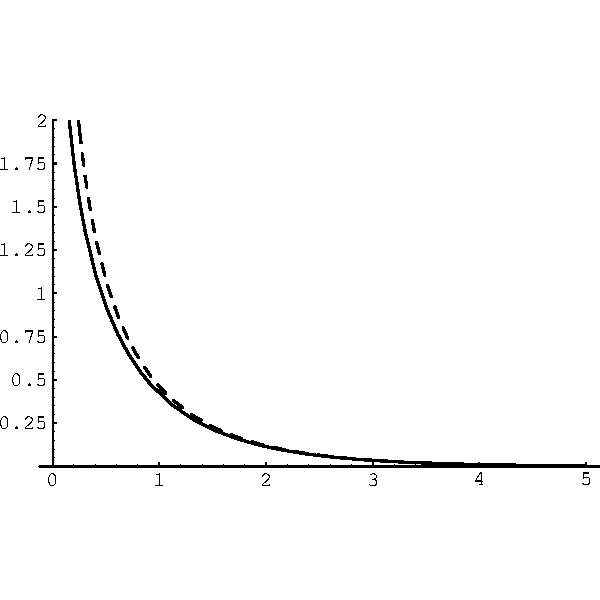
\includegraphics[width=0.6\textwidth]{ode/asymptotic/besselk0}
    \end{center}
    \caption{Plot of the modified Bessel function and its leading order 
      behavior.}
    \label{besselk0}
  \end{figure}

\end{Example}





















%%=============================================================================
\section{Integration by Parts}
\index{asymptotic expansions!integration by parts}

\begin{Example}
  \label{error_function}
  The complementary error function
  \[ \erfc(x) = \frac{2}{\sqrt{\pi}} \int_x^\infty \e^{-t^2}\,dt\]
  is used in statistics for its relation to the normal probability distribution.
  We would like to find an approximation to $\erfc(x)$ for large $x$.
  Using integration by parts,
  \begin{align*}
    \erfc(x)
    &= \frac{2}{\sqrt{\pi}}\int_x^\infty \left(\frac{-1}{2t}\right)
    \left(-2 t \e^{-t^2}\right)\,dt \\
    &= \frac{2}{\sqrt{\pi}}\left[\frac{-1}{2t}\e^{-t^2}\right]_x^\infty - 
    \frac{2}{\sqrt{\pi}}\int_x^\infty
    \frac{1}{2}t^{-2} \e^{-t^2}\,dt \\
    &= \frac{1}{\sqrt{\pi}}x^{-1} \e^{-x^2} - 
    \frac{1}{\sqrt{\pi}}\int_x^\infty t^{-2} \e^{-t^2}\,dt. 
  \end{align*}
  We examine the residual integral in this expression.
  \begin{align*}
    \frac{1}{\sqrt{\pi}} \int_x^\infty t^{-2} \e^{-t^2}\,dt
    &\leq \frac{-1}{2\sqrt{\pi}} x^{-3} \int_x^\infty -2t \e^{-t^2}\,dt \\
    &= \frac{1}{2\sqrt{\pi}} x^{-3} \e^{-x^2}.
  \end{align*}
  Thus we see that
  \[\frac{1}{\sqrt{\pi}}x^{-1} \e^{-x^2} \gg 
  \frac{1}{\sqrt{\pi}}\int_x^\infty t^{-2} \e^{-t^2}\,dt
  \quad \mathrm{as}\ x \to \infty. \]
  Therefore, 
  \[ \erfc(x) \sim \frac{1}{\sqrt{\pi}} x^{-1} \e^{-x^2}
  \quad \mathrm{as}\ x \to \infty,\]
  and we expect that $\frac{1}{\sqrt{\pi}}x^{-1} \e^{-x^2}$ would
  be a good approximation to $\erfc(x)$ for large $x$.
  In Figure~\ref{log_first_term} $\log(\erfc(x))$ is graphed in a solid line and
  $\log\left(\frac{1}{\sqrt{\pi}} x^{-1}\e^{-x^2}\right)$ 
  is graphed in a dashed line.
  We see that this first approximation to the error function gives very 
  good results even for moderate values of $x$.  Table~\ref{table_ltt} gives
  the error in this first approximation for various values of $x$.


  \begin{figure}[h!]
    \begin{center}
      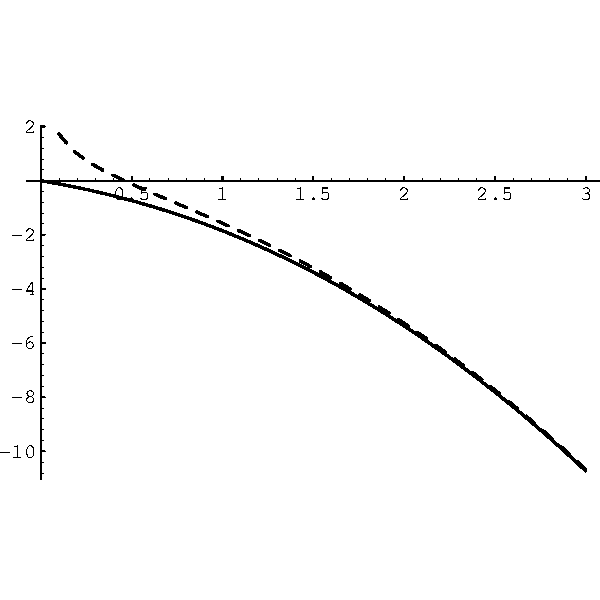
\includegraphics[width=0.6\textwidth]{ode/asymptotic/log_ft}
    \end{center}
    \caption{The logarithm of the approximation to the complementary error 
      function.}
    \label{log_first_term}
  \end{figure}




  If we continue integrating by parts, we might get a better approximation 
  to the complementary error function.
  \begin{align*}
    \erfc(x)
    &= \frac{1}{\sqrt{\pi}}x^{-1} \e^{-x^2} - 
    \frac{1}{\sqrt{\pi}}\int_x^\infty
    t^{-2} \e^{-t^2}\,dt \\
    &= \frac{1}{\sqrt{\pi}}x^{-1} \e^{-x^2} - 
    \frac{1}{\sqrt{\pi}}\left[-\frac{1}{2}t^{-3}\e^{-t^2}
    \right]_x^\infty
    + \frac{1}{\sqrt{\pi}}\int_x^\infty
    \frac{3}{2}t^{-4} \e^{-t^2}\,dt \\
    &= \frac{1}{\sqrt{\pi}}\e^{-x^2}\left(x^{-1} 
      - \frac{1}{2}x^{-3}\right)
    + \frac{1}{\sqrt{\pi}}\int_x^\infty
    \frac{3}{2}t^{-4} \e^{-t^2}\,dt \\
    &= \frac{1}{\sqrt{\pi}}\e^{-x^2}\left(x^{-1} 
      - \frac{1}{2}x^{-3}\right)
    + \frac{1}{\sqrt{\pi}}\left[-\frac{3}{4}t^{-5}\e^{-t^2}
    \right]_x^\infty
    - \frac{1}{\sqrt{\pi}}\int_x^\infty
    \frac{15}{4}t^{-6} \e^{-t^2}\,dt \\
    &= \frac{1}{\sqrt{\pi}}\e^{-x^2}\left(x^{-1} 
      - \frac{1}{2}x^{-3} + \frac{3}{4}x^{-5}\right)
    - \frac{1}{\sqrt{\pi}}\int_x^\infty
    \frac{15}{4}t^{-6} \e^{-t^2}\,dt 
  \end{align*}
  The error in approximating $\erfc(x)$ with the first three terms is
  given in Table~\ref{table_ltt}.
  We see that for $x \geq 2$ the three terms give a much better approximation
  to $\erfc(x)$ than just the first term.

  \begin{table}
    \[
    \begin{array}{llll}
      \mathbf{x}      &\mathbf{\berfc(x)}     
      & \mathrm{One Term Relative Error} \qquad
      & \mathrm{Three Term Relative Error} \\
      \hline
      1       &0.157                  &0.3203         &0.6497 \\
      2       &0.00468                &0.1044         &0.0182 \\
      3       &2.21\times 10^{-5}  &0.0507         &0.0020 \\
      4       &1.54\times 10^{-8}  &0.0296         &3.9 \cdot 10^{-4} \\
      5       &1.54\times 10^{-12} &0.0192         &1.1 \cdot 10^{-4}\\
      6       &2.15\times 10^{-17} &0.0135         &3.7 \cdot 10^{-5}\\
      7       &4.18\times 10^{-23} &0.0100         &1.5 \cdot 10^{-5}\\
      8       &1.12\times 10^{-29} &0.0077         &6.9 \cdot 10^{-6}\\
      9       &4.14\times 10^{-37} &0.0061         &3.4 \cdot 10^{-6}\\
      10 \quad &2.09\times 10^{-45}\quad &0.0049 
      &1.8 \cdot 10^{-6}
    \end{array}
    \]
    \caption{The error in approximating the complementary error function.}
    \label{table_ltt}
  \end{table}


  At this point you might guess that you could continue this process 
  indefinitely.  By repeated application of integration by parts, you can
  obtain the series expansion
  \[ \erfc(x) = \frac{2}{\sqrt{\pi}} \e^{-x^2} \sum_{n=0}^\infty 
  \frac{(-1)^n (2n)!}{n! (2x)^{2n+1}}.\]
  This is a Taylor expansion about infinity.  Let's find the radius of 
  convergence.
  \begin{align*}
    \lim_{n \to \infty} \left| \frac{a_{n+1}(x)}{a_n(x)}\right| < 1 
    &\to \lim_{n \to \infty} \left| \frac{(-1)^{n+1} (2(n+1))!}
      {(n+1)! (2x)^{2(n+1)+1}} \frac{n! (2x)^{2n+1}}{(-1)^n (2n)!}
    \right| < 1 \\
    &\to \lim_{n \to \infty} \left|\frac{(2n+2)(2n+1)}{(n+1)(2x)^2}\right|
    < 1 \\
    &\to \lim_{n \to \infty} \left|\frac{2(2n+1)}{(2x)^2}\right| < 1 \\
    &\to \left| \frac{1}{x}\right| = 0
  \end{align*}
  Thus we see that our series diverges for all $x$.  Our conventional 
  mathematical sense would tell us that this series is useless, however we
  will see that this series is very useful as an asymptotic expansion of
  $\erfc(x)$.  

  Say we are working with a convergent series expansion of some function $f(x)$.
  \[f(x) = \sum_{n=0}^\infty a_n(x)\]
  For fixed $x=x_0$, 
  \[ f(x_0) - \sum_{n=0}^N a_n(x_0) \to 0 \quad \mathrm{as}\ N \to \infty.\]
  For an asymptotic series we have a quite different behavior.
  If $g(x)$ is asymptotic to $\sum_{n = 0}^\infty b_n(x)$ as $x \to x_0$ then
  for fixed $N$,
  \[ g(x) - \sum_0^N b_n(x) \ll b_N(x) \quad \mathrm{as}\ x \to x_0. \]
  For the complementary error function,
  \[\mathrm{For fixed}\ N,\ \erfc(x) - \frac{2}{\sqrt{\pi}} \e^{-x^2} 
  \sum_{n=0}^N \frac{(-1)^n (2n)!}{n! (2x)^{2n+1}} \ll x^{-2N-1} \quad
  \mathrm{as}\ x \to \infty.\]
  We say that the error function is asymptotic to the series as $x$ goes to 
  infinity.
  \[ \erfc(x) \sim \frac{2}{\sqrt{\pi}} \e^{-x^2} \sum_{n=0}^\infty 
  \frac{(-1)^n (2n)!}{n! (2x)^{2n+1}} \quad \mathrm{as}\ x \to \infty\]

  In Figure~\ref{one_ten_twenty} the logarithm of the difference between the one
  term, ten term and twenty term approximations and the complementary
  error function are graphed in coarse, medium, and fine dashed lines,
  respectively.




  \begin{figure}[h!]
    \begin{center}
      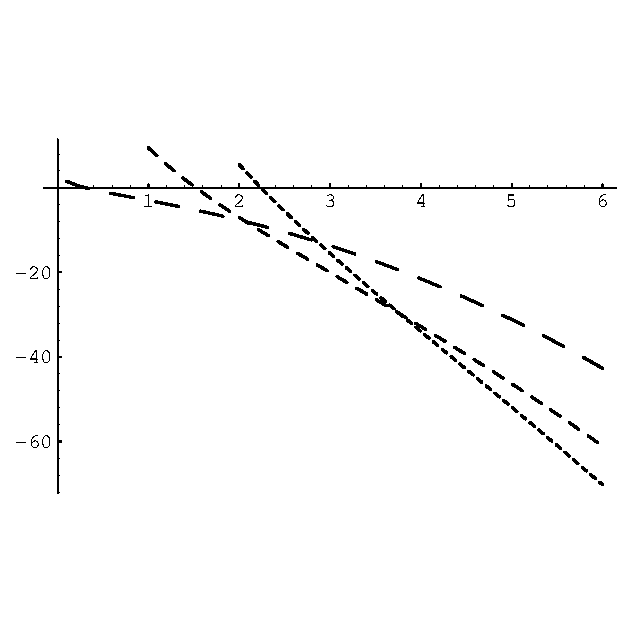
\includegraphics[width=0.6\textwidth]{ode/asymptotic/one1020}
    \end{center}
    \caption{The logarithm of the error in the approximation.}
    \label{one_ten_twenty}
  \end{figure}


  

  \paragraph{*Optimal Asymptotic Series.}
  Of the three approximations, the one term is best for $x \lesssim 2$,
  the ten term is best for $2 \lesssim x \lesssim 4$, and the twenty term
  is best for $4 \lesssim x$.  This leads us to the concept of an optimal
  asymptotic approximation.  An optimal asymptotic approximation contains 
  the number of terms in the series that best approximates the true 
  behavior.
  \index{optimal asymptotic approximations}

  In Figure~\ref{optimal} we see a plot of the number of terms in the
  approximation versus the logarithm of the error for $x = 3$.  Thus 
  we see that the optimal asymptotic approximation is the
  first nine terms.  After nine terms the error gets larger.  It was
  inevitable that the error would start to grow after some point as the
  series diverges for all $x$.


  \begin{figure}[h!]
    \begin{center}
      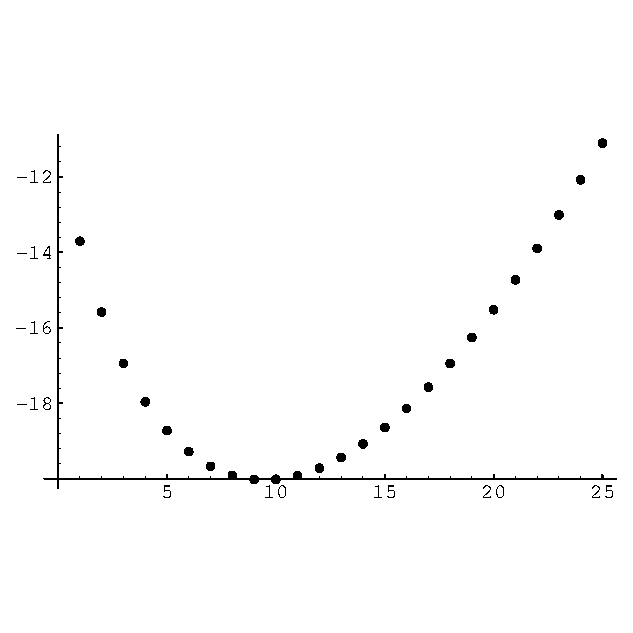
\includegraphics[width=0.6\textwidth]{ode/asymptotic/optimal}
    \end{center}
    \caption{The logarithm of the error.}
    \label{optimal}
  \end{figure}




  A good rule of thumb for finding the optimal series is to find the
  smallest term in the series and take all of the terms up to but not
  including the smallest term as the optimal approximation.  This
  makes sense, because the $n^{t h}$ term is an approximation of the
  error incurred by using the first $n-1$ terms.
  In Figure~\ref{log_nth_term} there is a plot of $n$ versus the
  logarithm of the $n^{t h}$ term in the asymptotic expansion of
  $\erfc(3)$.  We see that the tenth term is the smallest.
  Thus, in this case, our rule of thumb predicts the actual optimal series.




  \begin{figure}[h!]
    \begin{center}
      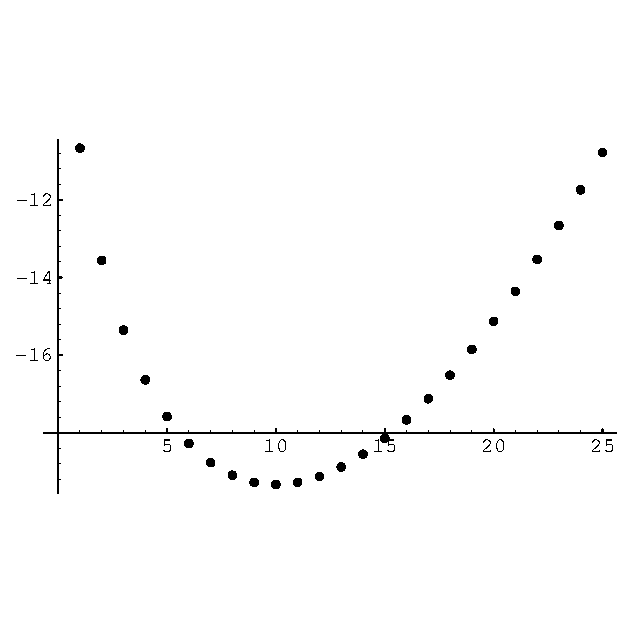
\includegraphics[width=0.6\textwidth]{ode/asymptotic/log_nt}
    \end{center}
    \caption{The logarithm of the terms in the expansion.}
    \label{log_nth_term}
  \end{figure}




\end{Example}




%%=============================================================================
\section{Asymptotic Series}

A function $f(x)$ has an asymptotic series expansion about $x=x_0$, 
$\sum_{n=0}^\infty a_n(x)$, if
\[ f(x) - \sum_{n=0}^N a_n(x) \ll a_N(x) \quad \mathrm{as}\ x \to x_0 \quad
\mathrm{for all}\ N.\]
An asymptotic series may be convergent or divergent.  Most of the 
asymptotic series you encounter will be divergent.  If the series is
convergent, then we have that
\[ f(x) - \sum_{n=0}^N a_n(x) \to 0 \quad \mathrm{as}\ N \to \infty
\quad \mathrm{for fixed}\ x.\]




Let $\epsilon_n(x)$ be some set of gauge functions.  The example that we 
are most familiar with is $\epsilon_n(x) = x^n$.  If we say that
\[ \sum_{n=0}^\infty a_n \epsilon_n(x) \sim 
\sum_{n=0}^\infty b_n \epsilon_n(x),\]
then this means that $a_n = b_n$.























%%=============================================================================
\section{Asymptotic Expansions of Differential Equations}










\subsection{The Parabolic Cylinder Equation.}

\paragraph{Controlling Factor.}
Let us examine the behavior of the bounded solution of the parabolic 
cylinder equation as $x \to + \infty$.  
\[ y'' + \left(\nu + \frac{1}{2} - \frac{1}{4} x^2\right)y = 0\]
This equation has an irregular singular point at infinity.  
With the substitution $y = \e^s$,
the equation becomes
\[s'' + (s')^2 + \nu + \frac{1}{2} - \frac{1}{4} x^2 = 0.\]
We know that 
\[ \nu + \frac{1}{2} \ll \frac{1}{4} x^2\quad \mathrm{as}\ x \to +\infty\]
so we drop this term from the equation. Let us make the assumption that
\[ s'' \ll (s')^2\quad \mathrm{as}\ x \to +\infty.\]
Thus we are left with the equation
\begin{eqnarray*}
  (s')^2 &\sim& \frac{1}{4} x^2 \\
  s' &\sim& \pm \frac{1}{2} x \\
  s &\sim& \pm \frac{1}{4} x^2 + c \\
  s &\sim& \pm \frac{1}{4} x^2\quad \mathrm{as}\ x \to +\infty
\end{eqnarray*}
Now let's check if our assumption is consistent.  Substituting into
$s'' \ll (s')^2$ yields $1/2 \ll x^2/4\quad \mathrm{as}\ x  \to +\infty$ which 
is true.  Since the equation for $y$ is second order, we would expect that 
there are two different behaviors as $x \to +\infty$.  This is 
confirmed by the fact that we found two behaviors for $s$.  $s \sim -x^2/4$
corresponds to the solution that is bounded at $+\infty$.
Thus the controlling factor of the leading behavior is $\e^{-x^2/4}$.



\paragraph{Leading Order Behavior.}
Now we attempt to get a better approximation to $s$. We make the substitution
$s = -\frac{1}{4} x^2 + t(x)$ into the equation for $s$ where 
$t \ll x^2$ as $x \to +\infty$.
\[ -\frac{1}{2} + t'' + \frac{1}{4} x^2 - x t' + (t')^2 + \nu + \frac{1}{2}
-\frac{1}{4} x^2 = 0 \]
\[ t'' - x t' + (t')^2 + \nu = 0 \]
Since $t \ll x^2$, we assume that $t' \ll x$ and $t'' \ll 1$ as 
$x \to +\infty$.  
Note that this in only an assumption since it is not always valid to
differentiate an asymptotic relation.
Thus $(t')^2 \ll x t'$ and $t'' \ll x t'$ as
$x \to +\infty$; we drop these terms from the equation.  
\begin{eqnarray*}
  t' &\sim& \frac{\nu}{x} \\
  t &\sim& \nu \log x + c \\
  t &\sim& \nu \log x\quad \mathrm{as}\ x \to +\infty
\end{eqnarray*}
Checking our assumptions for the derivatives of $t$,
\[ t' \ll x \quad \to \quad \frac{1}{x} \ll x \qquad \qquad
t'' \ll 1 \quad \to \quad \frac{1}{x^2} \ll 1,\]
we see that they were consistent.  Now we wish to refine our approximation for
$t$ with the substitution $t(x) = \nu \log x + u(x)$.
So far we have that 
\[ y \sim \exp\left[-\frac{x^2}{4} + \nu \log x + u(x)\right] 
= x^\nu \exp\left[-\frac{x^2}{4}+ u(x) \right] 
\quad  \mathrm{as}\ x \to +\infty. \]
We can try and determine $u(x)$ by substituting the expression
$t(x) = \nu \log x + u(x)$ into the equation for $t$. 
\[ -\frac{\nu}{x^2} + u'' - (\nu + x u') + \frac{\nu^2}{x^2} + 
\frac{2\nu}{x} u' + (u')^2 + \nu = 0\]
After suitable simplification, this equation becomes
\[ u' \sim \frac{\nu^2 - \nu}{x^3}\quad \mathrm{as}\ x \to +\infty \]
Integrating this asymptotic relation, 
\[ u \sim \frac{\nu-\nu^2}{2x^2} + c \quad \mathrm{as}\ x \to +\infty. \]
Notice that $\frac{\nu-\nu^2}{2x^2} \ll c$ as $x \to +\infty$;
thus this procedure fails to give us the behavior of $u(x)$.  Further 
refinements to our approximation for $s$ go to a constant value as 
$x \to +\infty$.  Thus we have that the leading behavior is
\[y \sim c x^\nu \exp\left[-\frac{x^2}{4} \right]
\quad \mathrm{as}\ x \to +\infty\]




\paragraph{Asymptotic Expansion}
Since we have factored off the singular behavior of $y$, we might expect that
what is left over is well behaved enough to be expanded in a Taylor series
about infinity. 
Let us assume that we can expand the solution for $y$ in the form
\[ y(x) \sim x^\nu \exp\left(-\frac{x^2}{4} \right) \sigma(x) = 
x^\nu \exp\left(-\frac{x^2}{4}\right) \sum_{n=0}^\infty a_n x^{-n}
\mathrm{as}\ x \to +\infty\]
where $a_0 = 1$.
Differentiating $y = x^\nu \exp\left(-\frac{x^2}{4} \right)\sigma(x)$,
\[ y' = \left[\nu x^{\nu-1} - \frac{1}{2} x^{\nu+1}\right]\e^{-x^2/4} \sigma(x) 
+ x^\nu \e^{-x^2/4} \sigma'(x) \]
\begin{align*} 
  y'' &= \left[\nu(\nu-1)x^{\nu-2} - \frac{1}{2}\nu x^\nu 
    - \frac{1}{2}(\nu+1)x^\nu
    +\frac{1}{4}x^{\nu+2}\right]\e^{-x^2/4}\sigma(x) + 
  2\left[\nu x^{\nu-1} - \frac{1}{2} x^{\nu+1}\right]
  \e^{-x^2/4} \sigma'(x) \\
  &\qquad + x^\nu \e^{-x^2/4} \sigma''(x).
\end{align*}
Substituting this into the differential equation for $y$,
\begin{gather*}
  \left[\nu(\nu-1)x^{-2} - (\nu+\frac{1}{2}) + \frac{1}{4} x^2\right]\sigma(x) + 
  2\left[\nu x^{-1} - \frac{1}{2} x\right]\sigma'(x) + \sigma''(x) + 
  \left[\nu + \frac{1}{2} - \frac{1}{4} x^2\right]\sigma(x) = 0 \\
  \sigma''(x) + (2\nu x^{-1} - x)\sigma'(x) + \nu(\nu-1) x^{-2} \sigma = 0 \\
  x^2 \sigma''(x) + (2\nu x - x^3)\sigma'(x) + \nu(\nu-1)\sigma(x) = 0.
\end{gather*}







Differentiating the expression for $\sigma(x)$,
\begin{align*}
  \sigma(x) &= \sum_{n=0}^\infty a_n x^{-n} \\
  \sigma'(x) &= \sum_{n=1}^\infty -n a_n x^{-n-1} 
  = \sum_{n=-1}^\infty -(n+2)a_{n+2} x^{-n-3} \\
  \sigma''(x) &= \sum_{n=1}^\infty n(n+1) a_n x^{-n-2}.
\end{align*}
Substituting this into the differential equation for $\sigma(x)$,
\[      \sum_{n=1}^\infty n(n+1) a_n x^{-n} + 
2\nu \sum_{n=1}^\infty -n a_n x^{-n} - 
\sum_{n=-1}^\infty -(n+2)a_{n+2} x^{-n} + 
\nu(\nu-1) \sum_{n=0}^\infty a_n x^{-n} = 0.
\]
Equating the coefficient of $x^1$ to zero yields
\[ a_1 x = 0\quad \to \quad a_1 = 0. \]
Equating the coefficient of $x^0$,
\[2 a_2 + \nu(\nu-1)a_0 = 0 \quad \to \quad 
a_2 = -\frac{1}{2}\nu(\nu-1).\]
From the coefficient of $x^{-n}$ for $n > 0$,
\begin{align*}
  n(n+1)a_n &- 2\nu n a_n + (n+2)a_{n+2} + \nu(\nu-1)a_n = 0 \\
  (n+2)a_{n+2} &= - [n(n+1) - 2\nu n + \nu(\nu-1)]a_n \\
  (n+2)a_{n+2} &= - [n^2 + n - 2\nu n + \nu(\nu-1)]a_n \\
  (n+2)a_{n+2} &= - (n-\nu)(n-\nu+1)a_n. 
\end{align*}







Thus the recursion formula for the $a_n$'s is
\[a_{n+2} = -\frac{(n-\nu)(n-\nu+1)}{n+2}a_n,\quad a_0 = 1,\ \ \ a_1 = 0. \]
The first few terms in $\sigma(x)$ are
\[\sigma(x) \sim 1 - \frac{\nu(\nu-1)}{2^1 1!}x^{-2} + 
\frac{\nu(\nu-1)(\nu-2)(\nu-3)}{2^2 2!} x^{-4} - \cdots \quad 
\mathrm{as}\ x  \to +\infty\]
If we check the radius of convergence of this series
\begin{align*}
  \lim_{n \to \infty} \left| \frac{a_{n+2} x^{-n-2}}{a_n x^{-n}}\right|<1 \quad
  &\to \quad \lim_{n \to \infty} \left| 
    -\frac{(n-\nu)(n-\nu+1)}{n+2} x^{-2} \right| < 1 \\
  &\to \quad \frac{1}{x} = 0
\end{align*}
we see that the radius of convergence is zero.  Thus if $\nu \neq 0,1,2,\ldots$
our asymptotic expansion for $y$
\[ y \sim x^\nu \e^{-x^2/4}\left[1 - \frac{\nu(\nu-1)}{2^1 1!}x^{-2} + 
  \frac{\nu(\nu-1)(\nu-2)(\nu-3)}{2^2 2!} x^{-4} - \cdots\right] \]
diverges for all x.  However this solution is still very useful. 
If we only use a finite number of terms, we will get a very good numerical 
approximation for large $x$.


In Figure~\ref{par_cyl} the one term, two term, and three term asymptotic
approximations are shown in rough, medium, and fine dashing, respectively.
The numerical solution is plotted in a solid line.

\begin{figure}[h!]
  \begin{center}
    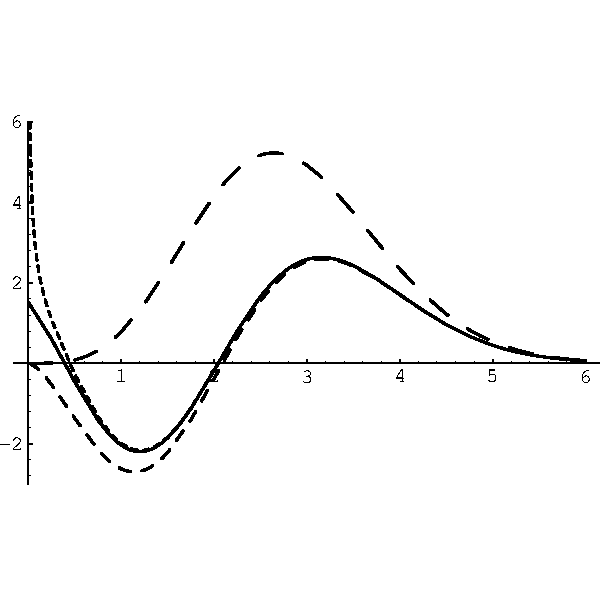
\includegraphics[width=0.6\textwidth]{ode/asymptotic/par_cyl}
  \end{center}
  \caption{Asymptotic approximations to the parabolic cylinder function.}
  \label{par_cyl}
\end{figure}












\flushbottom

%%
%% Add a graph to example 1.2.5, $\sign(x)$.
%%
%% Add a section on the inner product.  use some of the material in sug5.
%% Do vectors as an example.
%%




%%============================================================================
%%============================================================================
\chapter{Hilbert Spaces}





An expert is a man who has made all the mistakes which can be made, 
in a narrow field.

\begin{flushright}
  - Niels Bohr
\end{flushright}










%% CONTINUE
WARNING: UNDER HEAVY CONSTRUCTION.

In this chapter we will introduce Hilbert spaces.  We develop the two 
important examples: $l_2$, the space of square summable infinite vectors 
and $L_2$, the space of square integrable functions.







%% CONTINUE: this section may need some work
%%============================================================================
\section{Linear Spaces}
\index{linear space}


A \textit{linear space} is a set of elements $\{x, y, z, \ldots\}$
that is closed under addition and scalar multiplication.  By closed under 
addition we mean: if $x$ and $y$ are elements, then $z = x + y$ is an element.
The addition is commutative and associative.
\begin{gather*}
  x + y = y + x \\
  (x + y) + z = x + (y + z)
\end{gather*}
Scalar multiplication is associative and distributive.
Let $a$ and $b$ be scalars, $a,b \in \mathbb{C}$.
\begin{gather*}
  (a b) x = a (b x) \\
  (a + b) x = a x + b x \\
  a(x + y) = a x + a y
\end{gather*}

All the linear spaces that we will work with have additional properties:
The zero element $0$ is the additive identity.
\[
x + 0 = x
\]
Multiplication by the scalar $1$ is the multiplicative identity.
\[
1 x = x
\]
Each element $x$ and the additive inverse, $-x$.
\[
x + (-x) = 0
\]


Consider a set of elements $\{x_1, x_2, \ldots\}$.  Let the $c_i$ be scalars.
If 
\[
y = c_1 x_1 + c_2 x_2 + \cdots
\]
then $y$ is a \textit{linear combination} of the $x_i$.
A set of elements $\{x_1, x_2, \ldots\}$ is \textit{linearly independent} if 
the equation
\[
c_1 x_1 + c_2 x_2 + \cdots = 0
\]
has only the trivial solution $c_1 = c_2 = \cdots = 0$.  Otherwise the set
is \textit{linearly dependent}. 


Let $\{e_1, e_2, \cdots\}$ be a linearly independent set of elements.
If every element $x$ can be written as a linear combination of the $e_i$
then the set $\{ e_i \}$ is a \textit{basis} for the space.  
The $e_i$ are called \textit{base elements}.
\[
x = \sum_{i} c_i e_i
\]
The set $\{e_i\}$ is also called a \textit{coordinate system}.  The scalars
$c_i$ are the \textit{coordinates} or $\textit{components}$ of $x$.
If the set $\{e_i\}$ is a basis, then we say that the set is 
\textit{complete}.





%%\begin{Example}
%% CONTINUE: vectors
%%\end{Example}





%%\begin{Example}
%% CONTINUE: C^2 functions, 
%% C^2 functions which satisfy homogeneous or periodic boundary conditions
%% C^2 functions which satisfy inhom boundary conditions for a counter-example
%%\end{Example}












%% CONTINUE: this section may need some work
%%============================================================================
\section{Inner Products}


$\langle x | y \rangle$ is an \textit{inner product} of two elements $x$ and $y$ if it 
satisfies the properties:
\begin{enumerate}
  %%
\item
  Conjugate-commutative.
  \[
  \langle x | y \rangle = \overline{ \langle x | y \rangle }
  \]
  %%
\item
  Linearity in the second argument.
  \[
  \langle x | a y + b z \rangle = a \langle x | y \rangle + b \langle x | y \rangle
  \]
  %%
\item
  Positive definite.
  \begin{gather*}
    \langle x | x \rangle \geq 0 \\
    \langle x | x \rangle = 0\ \mathrm{if and only if}\ x = 0
  \end{gather*}
\end{enumerate}

From these properties one can derive the properties:
\begin{enumerate}
  %%
\item
  Conjugate linearity in the first argument.
  \[
  \langle a x + b y | z \rangle = \overline{a} \langle x | z \rangle + \overline{b} \langle x | z \rangle
  \]
  %%
\item
  Schwarz Inequality.
  \[
  \left| \langle x | y \rangle \right|^2 \leq \langle x | x \rangle \langle y | y \rangle
  \]
\end{enumerate}





One inner product of vectors is the \textit{Euclidean inner product}.
\[
\langle \mathbf{x} | \mathbf{y} \rangle \equiv \mathbf{x} \cdot \mathbf{y} = \sum_{i=0}^n \overline{x_i} y_i.
\]

One inner product of functions defined on $(a \ldots b)$ is
\[
\langle u | v \rangle = \int_a^b \overline{u(x)} v(x) \,\dd x.
\]
If $\sigma(x)$ is a positive-valued function, then we can define the
inner product:
\[
\langle u | \sigma| v \rangle = \int_a^b \overline{u(x)} \sigma(x) v(x) \,\dd x.
\]
This is called the inner product with respect to the weighting function 
$\sigma(x)$.  It is also denoted $\langle u | v \rangle_\sigma$.




%% CONTINUE: this section may need some work
%%============================================================================
\section{Norms}


A \textit{norm} is a real-valued function on a space which satisfies the
following properties.
\begin{enumerate}
\item
  Positive.
  \[
  \|x\| \geq 0
  \]
\item
  Definite.
  \[
  \|x\| = 0\ \mathrm{if and only if}\ x = 0
  \]
\item
  Multiplication my a scalar, $c \in \mathbb{C}$.
  \[
  \| c x \| = |c| \|x \|
  \]
\item
  Triangle inequality.
  \[
  \|x + y\| \leq \|x\| + \|y\|
  \]
\end{enumerate}




\begin{Example}
  Consider a vector space, (finite or infinite dimension), with elements
  $x = (x_1, x_2, x_3, \ldots)$.  Here are some common norms.
  \begin{itemize}
  \item
    Norm generated by the inner product.
    \[
    \|x\| = \sqrt{\langle x | x \rangle}
    \]
  \item
    The $l_p$ norm.
    \[
    \|x\|_p = \left( \sum_{k = 1}^\infty |x_k|^p \right)^{1/p}
    \]
    There are three common cases of the $l_p$ norm.
    \begin{itemize}
    \item
      Euclidian norm, or $l_2$ norm.
      \[
      \|x\|_2 = \sqrt{ \sum_{k = 1}^\infty |x_k|^2 }
      \]
    \item
      $l_1$ norm.
      \[
      \|x\|_1 = \sum_{k = 1}^\infty |x_k|
      \]
    \item
      $l_\infty$ norm.
      \[
      \|x\|_\infty = \max_k |x_k|
      \]
    \end{itemize}
  \end{itemize}
\end{Example}






\begin{Example}
  Consider a space of functions defined on the interval $(a \ldots b)$.
  Here are some common norms.
  \begin{itemize}
  \item
    Norm generated by the inner product.
    \[
    \|u\| = \sqrt{\langle u | u \rangle}
    \]
  \item
    The $L_p$ norm.
    \[
    \|u\|_p = \left( \int_a^b |u(x)|^p \,\dd x \right)^{1/p}
    \]
    There are three common cases of the $L_p$ norm.
    \begin{itemize}
    \item
      Euclidian norm, or $L_2$ norm.
      \[
      \|u\|_2 = \sqrt{ \int_a^b |u(x)|^2 \,\dd x }
      \]
    \item
      $L_1$ norm.
      \[
      \|u\|_1 = \int_a^b |u(x)| \,\dd x
      \]
    \item
      $L_\infty$ norm.
      \[
      \|u\|_\infty = \limsup_{x \in (a \ldots b)} |u(x)|
      \]
    \end{itemize}
  \end{itemize}
\end{Example}




%% CONTINUE


\paragraph{Distance.}
Using the norm, we can define the distance between elements $u$ and $v$.
\[
d(u,v) \equiv \|u - v \|
\]
Note that $d(u,v) = 0$ does not necessarily imply that $u = v$.
CONTINUE.



%% CONTINUE: Write
%%============================================================================
\section{Linear Independence.}

%%Define linear independence, span, etc.
%%Cover projections onto a subspace.
%%project sin(x) onto the space {1,x,...,x^n}
%%CONTINUE.




%% CONTINUE: Write
%%============================================================================
\section{Orthogonality}

%%Show how orthogonality is better than linear independence.
%%CONTINUE.

Orthogonality.
\[
\langle \phi_j | \phi_k \rangle = 0\ \mathrm{if}\ j \neq k
\]

Orthonormality.
\[
\langle \phi_j | \phi_k \rangle = \delta_{j k}
\]



\begin{Example}
  Infinite vectors.
  $e_j$ has all zeros except for a 1 in the $j^{\mathrm{th}}$ position. 
  \[
  e_j = (0, 0, \ldots 0, 1, 0, \ldots)
  \]
  %% CONTINUE HERE
\end{Example}



\begin{Example}
  $L_2$ functions on $(0 \ldots 2 \pi)$.
  \[
  \phi_j = \frac{1}{\sqrt{2\pi}} \e^{\imath j x}, \quad j \in \mathbb{Z}
  \]
  \[
  \phi_0 = \frac{1}{\sqrt{2\pi}}, \quad
  \phi_j^{(1)} = \frac{1}{\sqrt{\pi}} \cos(j x), \quad
  \phi_j^{(1)} = \frac{1}{\sqrt{\pi}} \sin(j x), \quad j \in \mathbb{Z}^+
  \]
  %% CONTINUE HERE
\end{Example}



%%The sine series is complete on (0...\pi), but not on (-\pi...\pi).
%% CONTINUE HERE





%% CONTINUE HERE




%%============================================================================
\section{Gramm-Schmidt Orthogonalization}
\index{Gramm-Schmidt orthogonalization}

Let $\{\psi_1(x), \ldots, \psi_n(x)\}$ be a set of linearly independent 
functions.  Using the Gramm-Schmidt orthogonalization process we can
construct a set of orthogonal functions $\{\phi_1(x), \ldots, \phi_n(x)\}$
that has the same span as the set of $\psi_n$'s with the formulas
\begin{align*}
  \phi_1 &= \psi_1 \\
  \phi_2 &= \psi_2 - \frac{\langle \phi_1 | \psi_2 \rangle}{\|\phi_1\|^2} \phi_1\\
  \phi_3 &= \psi_3 - \frac{\langle \phi_1 | \psi_3 \rangle}{\|\phi_1\|^2} \phi_1 
  - \frac{\langle \phi_2 | \psi_3 \rangle}{\|\phi_2\|^2} \phi_2\\
  \cdots & \\
  \phi_n &= \psi_n - \sum_{j=1}^{n-1} \frac{\langle \phi_j | \psi_n \rangle}
  {\|\phi_j\|^2} \phi_j.
\end{align*}

You could verify that the $\phi_m$ are orthogonal with a proof by induction.




\begin{Example}
  Suppose we would like a polynomial approximation to $\cos(\pi x)$ in the
  domain $[-1,1]$.  One way to do this is to find the Taylor expansion of 
  the function about $x=0$.  Up to terms of order $x^4$, this is
  \[ 
  \cos(\pi x) = 1 - \frac{(\pi x)^2}{2} + \frac{(\pi x)^4}{24} + O(x^6).
  \]
  In the first graph of Figure~\ref{least_cos} $\cos(\pi x)$ and this fourth 
  degree polynomial are plotted.
  We see that the approximation is very good near $x=0$, but deteriorates
  as we move away from that point.  This makes sense because the Taylor
  expansion only makes use of information about the function's behavior
  at the point $x=0$.

  As a second approach, we could find the least squares fit of a fourth
  degree polynomial to $\cos(\pi x)$.  The set of functions
  $\{1, x, x^2, x^3, x^4\}$ is independent, but not orthogonal in the interval
  $[-1,1]$.  Using Gramm-Schmidt orthogonalization,
  \begin{align*}
    \phi_0 &= 1 \\
    \phi_1 &= x - \frac{\langle 1 | x \rangle}{\langle 1 | 1 \rangle} = x \\
    \phi_2 &= x^2 - \frac{\langle 1 | x^2 \rangle}{\langle 1 | 1 \rangle}
    - \frac{\langle x | x^2 \rangle}{\langle x | x \rangle}x = x^2 - \frac{1}{3} \\
    \phi_3 &= x^3 - \frac{3}{5} x \\
    \phi_4 &= x^4 - \frac{6}{7}x^2 - \frac{3}{35}
  \end{align*}
  A widely used set of functions in mathematics is the set of 
  \textbf{Legendre polynomials} $\{P_0(x), P_1(x), \ldots\}$.
  \index{Legendre polynomials}
  They differ from the $\phi_n$'s that we generated only by constant factors.
  The first few are
  \begin{align*}
    P_0(x) &= 1 \\
    P_1(x) &= x \\
    P_2(x) &= \frac{3x^2 - 1}{2} \\
    P_3(x) &= \frac{5x^3 - 3x}{2} \\
    P_4(x) &= \frac{35x^4 - 30x^2 + 3}{8}.
  \end{align*}

  Expanding $\cos(\pi x)$ in Legendre polynomials
  \[ \cos(\pi x) \approx \sum_{n=0}^4 c_n P_n(x), \]
  and calculating the generalized Fourier coefficients with the formula
  \[ c_n = \frac{\langle P_n | \cos(\pi x) \rangle}{\langle P_n | P_n \rangle}, \]
  yields 
  \begin{align*}
    \cos(\pi x) &\approx - \frac{15}{\pi^2} P_2(x) + \frac{45(2\pi^2-21)}{\pi^4}
    P_4(x) \\
    &= \frac{105}{8\pi^4} [(315-30\pi^2)x^4 + (24\pi^2 - 270)x^2 + 
    (27 - 2\pi^2)]
  \end{align*}
  The cosine and this polynomial are plotted in the second graph in
  Figure~\ref{least_cos}.  The least squares fit method uses information
  about the function on the entire interval.  We see that the least
  squares fit does not give as good an approximation close to the
  point $x=0$ as the Taylor expansion.  However, the least squares fit gives a
  good approximation on the entire interval.  

  In order to expand a function in a Taylor series, the function must be analytic
  in some domain.  One advantage of using the method of least squares is that the
  function being approximated does not even have to be continuous.

  \begin{figure}[h!]
    \begin{center}
      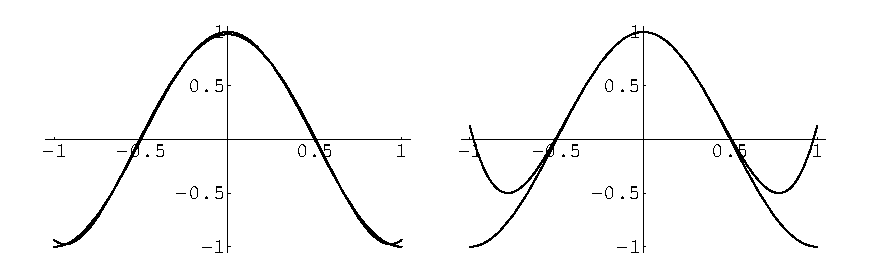
\includegraphics[width=\textwidth]{ode/hilbert/least}
    \end{center}
    \caption{Polynomial approximations of the function.}
    \label{least_cos}
  \end{figure}


\end{Example}





%% CONTINUE: Complete this.
%%============================================================================
\section{Orthonormal Function Expansion}

Let $\{\phi_j\}$ be an orthonormal set of functions
on the interval $(a,b)$.  We expand a function $f(x)$ in the $\phi_j$.
\[
f(x) = \sum_j c_j \phi_j
\]
We choose the coefficients to minimize the norm of the error.
\begin{align*}
  \left\| f - \sum_j c_j \phi_j \right\|^2 
  &= \left\langle f - \sum_j c_j \phi_j \bigg| 
    f - \sum_j c_j \phi_j \right\rangle \\
  &= \| f \|^2 
  - \left\langle f \bigg| \sum_j c_j \phi_j \right\rangle
  - \left\langle \sum_j c_j \phi_j \bigg| f \right\rangle
  + \left\langle \sum_j c_j \phi_j \bigg| 
    \sum_j c_j \phi_j \right\rangle \\
  &= \| f \|^2 + \sum_j |c_j|^2
  - \sum_j c_j \langle f | \phi_j \rangle
  - \sum_j \overline{c_j} \langle \phi_j | f \rangle 
\end{align*}
\begin{equation}
  \label{eqn_f2_sjcjpjf}
  \left\| f - \sum_j c_j \phi_j \right\|^2 
  = \| f \|^2 + \sum_j |c_j|^2
  - \sum_j c_j \overline{\langle \phi_j | f \rangle}
  - \sum_j \overline{c_j} \langle \phi_j | f \rangle
\end{equation}
To complete the square, we add the constant 
$\sum_j \langle \phi_j | f \rangle \overline{ \langle \phi_j | f \rangle }$.
We see the values of $c_j$ which minimize
\[
\| f \|^2 + \sum_j \left| c_j - \langle \phi_j | f \rangle \right|^2.
\]
Clearly the unique minimum occurs for
\[
c_j = \langle \phi_j | f \rangle.
\]
We substitute this value for $c_j$ into the right side of 
Equation~\ref{eqn_f2_sjcjpjf} and note that this quantity, the squared norm
of the error, is non-negative.
\begin{gather*}
  \| f \|^2 + \sum_j |c_j|^2 - \sum_j |c_j|^2 - \sum_j |c_j|^2 \geq 0 \\
  \| f \|^2 \geq \sum_j |c_j|^2 
\end{gather*}
This is known as \textit{Bessel's Inequality}.  If the set of $\{\phi_j\}$ is 
complete then the norm of the error is zero and we obtain 
\textit{Bessel's Equality}.
\[
\| f \|^2 = \sum_j |c_j|^2 
\]
%% CONTINUE HERE: unitary transformations, Parseval's relation.






%% CONTINUE: slice this up and fold it into the chapter.
%%============================================================================
\section{Sets Of Functions}

\paragraph{Orthogonality.}
Consider two complex valued functions of a real variable
$\phi_1(x)$ and $\phi_2(x)$ defined
on the interval $a \leq x \leq b$.  The inner product of the two functions
is defined
\index{inner product!of functions}
\[ \langle \phi_1 | \phi_2 \rangle = \int_a^b \overline{\phi_1}(x) \phi_2(x)\,\dd x.\]
The two functions are orthogonal if $\langle \phi_1 | \phi_2 \rangle = 0$.  The $L_2$
norm of a function is defined $\| \phi \| = \sqrt{\langle \phi | \phi \rangle}$.
\index{norm!of functions}

Let $\{ \phi_1, \phi_2, \phi_3, \ldots\}$ be a set of complex valued
functions.  The set of functions is orthogonal if each pair of functions
is orthogonal.  That is,
\[ \langle \phi_n | \phi_m \rangle = 0 \quad \mathrm{if}\ n \neq m.\]
If in addition the norm of each function is $1$, then the set is orthonormal.
\index{orthonormal}
That is,
\[ \langle \phi_n | \phi_m \rangle = \delta_{nm} = 
\begin{cases}
  1 \quad &\mathrm{if}\ n = m \\
  0 \quad &\mathrm{if}\ n \neq m.
\end{cases}
\]


\begin{Example}
  The set of functions
  \[ \left\{ \sqrt{\frac{2}{\pi}} \sin(x), \sqrt{\frac{2}{\pi}} \sin(2 x),
    \sqrt{\frac{2}{\pi}} \sin(3 x), \ldots \right\} \]
  is orthonormal on the interval $[0, \pi]$.
  To verify this,
  \begin{align*}
    \left\langle \sqrt{\frac{2}{\pi}} \sin(n x) \Bigg| 
      \sqrt{\frac{2}{\pi}} \sin(n x) \right\rangle
    &= \frac{2}{\pi} \int_0^\pi \sin^2(n x)\,\dd x \\
    &= 1
  \end{align*}
  If $n \neq m$ then
  \begin{align*}
    \left\langle \sqrt{\frac{2}{\pi}} \sin(n x) \Bigg| 
      \sqrt{\frac{2}{\pi}} \sin(m x) \right\rangle
    &= \frac{2}{\pi} \int_0^\pi \sin(n x) \sin(m x)\,\dd x \\
    &= \frac{1}{\pi} \int_0^\pi (\cos[(n-m)x] - \cos[(n+m)x])\,\dd x \\
    &= 0.
  \end{align*}
\end{Example}








\begin{Example}
  The set of functions
  \[ \{ \ldots, \frac{1}{\sqrt{2\pi}} \e^{-\imath x}, \frac{1}{\sqrt{2\pi}}, 
  \frac{1}{\sqrt{2\pi}} \e^{\imath x}, \frac{1}{\sqrt{2\pi}} \e^{\imath 2 x},
  \ldots \}, \]
  is orthonormal on the interval $[-\pi, \pi]$.
  To verify this,
  \begin{align*}
    \left\langle \frac{1}{\sqrt{2\pi}} \e^{\imath n x} \Bigg| \frac{1}{\sqrt{2\pi}}
      \e^{\imath n x} \right\rangle
    &= \frac{1}{2\pi} \int_{-\pi}^\pi \e^{-\imath n x} \e^{\imath n x}\,\dd x \\
    &= \frac{1}{2\pi} \int_{-\pi}^\pi \,\dd x \\
    &= 1.
  \end{align*}
  If $n \neq m$ then
  \begin{align*}
    \left\langle \frac{1}{\sqrt{2\pi}} \e^{\imath n x} \Bigg| \frac{1}{\sqrt{2\pi}}
      \e^{\imath m x} \right\rangle
    &= \frac{1}{2\pi} \int_{-\pi}^\pi \e^{-\imath n x} \e^{\imath m x}\,\dd x \\
    &= \frac{1}{2\pi} \int_{-\pi}^\pi \e^{\imath (m - n) x}\,\dd x \\
    &= 0.
  \end{align*} 
\end{Example}














\paragraph{Orthogonal with Respect to a Weighting Function.}
\index{orthogonality!weighting functions}

Let $\sigma(x)$ be a real-valued, positive function on the 
interval $[a,b]$.  We introduce the notation
\[ \langle \phi_n | \sigma | \phi_m \rangle \equiv \int_a^b \overline{\phi_n}
\sigma \phi_m\, d x.\]
If the set of functions $\{\phi_1, \phi_2, \phi_3, \ldots\}$ satisfy 
\[ \langle \phi_n | \sigma | \phi_m \rangle = 0 \quad \mathrm{if}\ n \neq m \]
then the functions are orthogonal with respect to the weighting function
$\sigma(x)$. 

If the functions satisfy
\[ \langle \phi_n | \sigma | \phi_m \rangle = \delta_{nm} \]
then the set is orthonormal with respect to $\sigma(x)$.



\begin{Example}
  We know that the set of functions
  \[ \left\{ \sqrt{\frac{2}{\pi}} \sin(x), \sqrt{\frac{2}{\pi}} \sin(2 x),
    \sqrt{\frac{2}{\pi}} \sin(3 x), \ldots \right\} \]
  is orthonormal on the interval $[0, \pi]$.
  That is,
  \[ \int_0^\pi \sqrt{\frac{2}{\pi}} \sin(n x) 
  \sqrt{\frac{2}{\pi}} \sin(m x) \,\dd x = \delta_{nm}. \]
  If we make the change of variables $x = \sqrt{t}$ in this integral, we obtain
  \[ \int_0^{\pi^2} \frac{1}{2\sqrt{t}} \sqrt{\frac{2}{\pi}} \sin(n \sqrt{t})
  \sqrt{\frac{2}{\pi}} \sin(m \sqrt{t})\, d t = \delta_{nm}.\]
  Thus the set of functions
  \[ \left\{ \sqrt{\frac{1}{\pi}} \sin(\sqrt{t}), \sqrt{\frac{1}{\pi}} \sin(2\sqrt{t}),
    \sqrt{\frac{1}{\pi}} \sin(3\sqrt{t}), \ldots \right\} \]
  is orthonormal with respect to $\sigma(t) = \frac{1}{2 \sqrt{t}}$ on the interval
  $[0, \pi^2]$.
\end{Example}







\paragraph{Orthogonal Series.}
\index{orthogonal series}
Suppose that a function $f(x)$ defined on $[a,b]$
can be written as a uniformly convergent sum of functions that are 
orthogonal with respect to $\sigma(x)$.
\[ f(x) = \sum_{n = 1}^\infty c_n \phi_n(x) \]
We can solve for the $c_n$ by taking the inner product of $\phi_m(x)$ and 
each side of the equation with respect to $\sigma(x)$. 
\begin{gather*}
  \langle \phi_m | \sigma | f \rangle = \left\langle \phi_m \Bigg| \sigma \Bigg| 
    \sum_{n = 1}^\infty c_n \phi_n \right\rangle \\
  \langle \phi_m | \sigma | f \rangle = \sum_{n = 1}^\infty c_n \langle \phi_m | \sigma | \phi_n 
  \rangle \\
  \langle \phi_m | \sigma | f \rangle = c_m \langle \phi_m | \sigma | \phi_m \rangle \\
  c_m = \frac{\langle \phi_m | \sigma | f \rangle}{\langle \phi_m  | \sigma | \phi_m \rangle}
\end{gather*}
The $c_m$ are known as \textbf{Generalized Fourier coefficients}.
\index{Fourier coefficients}
If the functions in the expansion are orthonormal, the formula simplifies
to
\[ c_m = \langle \phi_m | \sigma | f \rangle. \]














\begin{Example}
  The function $f(x) = x(\pi - x)$ has a uniformly convergent series
  expansion in the domain $[0,\pi]$ of the form
  \[ x(\pi - x) = \sum_{n = 1}^\infty c_n \sqrt{\frac{2}{\pi}} \sin(n x).\]
  The Fourier coefficients are
  \begin{align*}
    c_n     &= \left\langle \sqrt{\frac{2}{\pi}} \sin(n x) \Bigg| x(\pi-x) \right\rangle \\
    &= \sqrt{\frac{2}{\pi}} \int_0^\pi x(\pi-x) \sin(n x)\,\dd x \\
    &= \sqrt{\frac{2}{\pi}} \frac{2}{n^3} (1 - (-1)^n) \\
    &= 
    \begin{cases}
      \sqrt{\frac{2}{\pi}} \frac{4}{n^3} \quad &\mathrm{for odd}\ n \\
      0 \quad &\mathrm{for even}\ n
    \end{cases}
  \end{align*}
  Thus the expansion is
  \[ x(\pi-x) = \sum_{\substack{ {n} = 1 \\ \mathrm{odd}\ n}}^{\infty} \frac{8}{\pi n^3} \sin(n x) \quad \mathrm{for}\ x \in [0, \pi]. \]

  In the first graph of Figure~\ref{sin_par} the first term in the expansion
  is plotted in a dashed line and $x (\pi - x)$ is plotted in a solid line.
  The second graph shows the two term approximation.

  \begin{figure}[h!]
    \begin{center}
      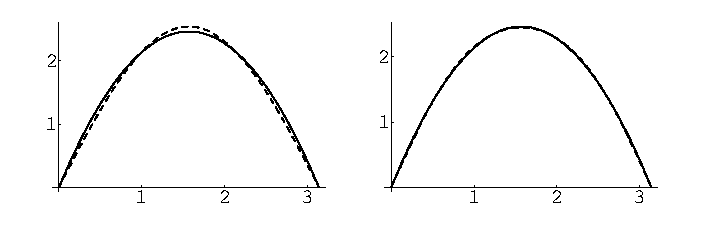
\includegraphics[width=\textwidth]{ode/hilbert/sin_par}
    \end{center}
    \caption{Series expansions of the function.}
    \label{sin_par}
  \end{figure}

\end{Example}












\begin{Example}
  The set $\{ \ldots, 1/\sqrt{2\pi} \e^{-\imath x}, 1/\sqrt{2\pi}, 
  1/\sqrt{2\pi} \e^{\imath x}, 1/\sqrt{2\pi} \e^{\imath 2 x}, \ldots\}$ is orthonormal
  on the interval $[-\pi,\pi]$.  $f(x) = \sign(x)$ has the
  expansion
  \begin{align*}
    \sign(x) 
    &\sim \sum_{n = -\infty}^\infty \left\langle \frac{1}{\sqrt{2\pi}} \e^{\imath n \xi} \Bigg| \sign(\xi) \right\rangle
    \frac{1}{\sqrt{2\pi}} \e^{\imath n x} \\
    &= \frac{1}{2\pi} \sum_{n = -\infty}^\infty \int_{-\pi}^\pi \e^{-\imath n \xi} \sign(\xi)
    \,\dd \xi \e^{\imath n x} \\
    &= \frac{1}{2\pi} \sum_{n = -\infty}^\infty \left( \int_{-\pi}^0 - \e^{-\imath n \xi}\,\dd \xi
      + \int_0^\pi \e^{-\imath n \xi}\,\dd \xi \right)
    \e^{\imath n x} \\
    &= \frac{1}{\pi} \sum_{n = -\infty}^\infty \frac{1 - (-1)^n}{\imath n} \e^{\imath n x}. \\
    \intertext{In terms of real functions, this is}
    &= \frac{1}{\pi} \sum_{n = -\infty}^\infty \frac{1 - (-1)^n}{\imath n} 
    (\cos(n x) + \imath \sin(n x)) \\
    &= \frac{2}{\pi} \sum_{n = 1}^\infty \frac{1 - (-1)^n}{\imath n} \sin(n x) 
  \end{align*}
  \[ \boxed{ \sign(x) \sim \frac{4}{\pi} \sum_{\substack{ {n} = 1 \\ \mathrm{odd}\ n}}^{\infty} 
    \frac{1}{n} \sin(n x).} \]
\end{Example}







%% CONTINUE: slice this up and fold it into the chapter.
%%============================================================================
\section{Least Squares Fit to a Function and Completeness}

Let $\{\phi_1, \phi_2, \phi_3, \ldots \}$ be a set of real, square integrable
functions that are orthonormal with respect to the weighting function
$\sigma(x)$ on the interval $[a, b]$.  That is,
\[ \langle \phi_n | \sigma | \phi_m \rangle = \delta_{nm}. \]
Let $f(x)$ be some square integrable function defined on the same interval.
We would like to approximate the function $f(x)$ with a finite
orthonormal series.
\[ 
f(x) \approx \sum_{n=1}^N \alpha_n \phi_n(x) 
\]
$f(x)$ may or may not have a uniformly convergent expansion in the orthonormal
functions.

We would like to choose the $\alpha_n$ so that we get the best possible
approximation to $f(x)$.  The most common measure of how well a series
approximates a function is the least squares measure.  The error 
is defined as the integral of the weighting function times the 
square of the deviation.
\[ 
E = \int_a^b \sigma(x) \left( f(x) - \sum_{n=1}^N \alpha_n \phi_n(x) \right)^2\,\dd x 
\]
The ``best'' fit is found by choosing the $\alpha_n$ that minimize $E$.
Let $c_n$ be the Fourier coefficients of $f(x)$.
\[ 
c_n = \langle \phi_n | \sigma | f \rangle
\]
we expand the integral for $E$.
\begin{align*}
  E(\alpha)
  &= \int_a^b \sigma(x) \left( f(x) - \sum_{n=1}^N \alpha_n \phi_n(x) \right)^2\,\dd x 
  \\
  &= \biggl\langle f - \sum_{n=1}^N \alpha_n \phi_n \biggm| \sigma \biggm|
  f - \sum_{n=1}^N \alpha_n \phi_n \biggr\rangle 
  \\
  &= \langle f | \sigma | f \rangle 
  - 2 \bigg\langle \sum_{n=1}^N \alpha_n \phi_n \bigg| \sigma \bigg| f \bigg\rangle
  + \bigg\langle \sum_{n=1}^N \alpha_n \phi_n \bigg| \sigma \bigg| 
  \sum_{n=1}^N \alpha_n \phi_n \bigg\rangle 
  \\
  &= \langle f | \sigma | f \rangle 
  -2 \sum_{n=1}^N \alpha_n \langle \phi_n | \sigma | f \rangle
  + \sum_{n=1}^N \sum_{m=1}^N \alpha_n \alpha_m \langle \phi_n | \sigma | \phi_m \rangle 
  \\
  &= \langle f | \sigma | f \rangle - 2 \sum_{n=1}^N \alpha_n c_n
  + \sum_{n=1}^N \alpha_n^2 
  \\
  &= \langle f | \sigma | f \rangle + \sum_{n=1}^N (\alpha_n - c_n)^2 - \sum_{n=1}^N c_n^2
\end{align*}
Each term involving $\alpha_n$ in non-negative and is minimized for $\alpha_n = c_n$.
The Fourier coefficients give the least squares approximation to a function.
The least squares fit to $f(x)$ is thus
\[ 
f(x) \approx \sum_{n=1}^N \langle \phi_n | \sigma | f \rangle\, \phi_n(x). \]


\begin{Result}
  If $\{\phi_1, \phi_2, \phi_3, \ldots\}$ is a set of real, square integrable
  functions that are orthogonal with respect to $\sigma(x)$
  then the least squares fit of the first $N$ 
  orthogonal functions to the square integrable function $f(x)$ is
  \[ 
  f(x) \approx \sum_{n=1}^N \frac{\langle \phi_n | \sigma | f \rangle}
  {\langle \phi_n | \sigma | \phi_n \rangle} \phi_n(x).
  \]
  If the set is orthonormal, this formula reduces to
  \[ 
  f(x) \approx \sum_{n=1}^N \langle \phi_n | \sigma | f  \rangle\, \phi_n(x).
  \]
\end{Result}



Since the error in the approximation $E$ is a nonnegative number we can
obtain on inequality on the sum of the squared coefficients.
\begin{gather*}
  E = \langle f | \sigma | f \rangle - \sum_{n=1}^N c_n^2 \\
  \boxed{ \sum_{n=1}^N c_n^2 \leq \langle f | \sigma | f \rangle }
\end{gather*}
This equation is known as \textbf{Bessel's Inequality}.
\index{Bessel's Inequality}
Since $\langle f | \sigma | f \rangle$ is just a nonnegative number, independent
of $N$, the sum $\sum_{n = 1}^\infty c_n^2$ is convergent and $c_n \to 0$ as 
$n \to \infty$

\paragraph{Convergence in the Mean.}
\index{convergence!in the mean}
If the error $E$ goes to zero as $N$ tends to infinity
\[ 
\lim_{N \to \infty} \int_a^b \sigma(x) \left( f(x) - \sum_{n=1}^N c_n \phi_n(x) \right)^2 \, d x = 0,
\]
then the sum converges in the mean to $f(x)$ relative to the weighting 
function $\sigma(x)$.  This implies that
\begin{gather*}
  \lim_{N \to \infty} \left( \langle f | \sigma | f \rangle - \sum_{n=1}^N c_n^2 \right) = 0 
  \\
  \boxed{
    \sum_{n = 1}^\infty c_n^2 = \langle f | \sigma | f \rangle.
    }
\end{gather*}
This is known as \textbf{Parseval's identity}.

\paragraph{Completeness.}
\index{completeness!of sets of functions}
Consider a set of functions $\{ \phi_1, \phi_2, \phi_3, \ldots\}$ that is
orthogonal with respect to the weighting function $\sigma(x)$.
If every function $f(x)$ that is square integrable with respect to
$\sigma(x)$ has an orthogonal series expansion
\[ f(x) \sim \sum_{n = 1}^\infty c_n \phi_n(x) \]
that converges in the mean to $f(x)$, then the set is \textbf{complete}.






%%============================================================================
\section{Closure Relation}
\index{closure relation!discrete sets of functions}

Let $\{ \phi_1, \phi_2, \ldots \}$ be an orthonormal, complete set on the
domain $[a,b]$.  For any
square integrable function $f(x)$ we can write
\[ f(x) \sim \sum_{n = 1}^\infty c_n \phi_n(x).\]
Here the $c_n$ are the generalized Fourier coefficients and the sum converges
in the mean to $f(x)$.  Substituting the expression for the Fourier
coefficients into the sum yields
\begin{align*}
  f(x) &\sim \sum_{n = 1}^\infty \langle \phi_n | f \rangle \phi_n(x) \\
  &= \sum_{n = 1}^\infty \left( \int_a^b \overline{\phi_n(\xi)} f(\xi)\,\dd \xi 
  \right) \phi_n(x). \\
  \intertext{Since the sum is not necessarily uniformly convergent, we are
    not justified in exchanging the order of summation and integration\ldots but
    what the heck, let's do it anyway.}
  &= \int_a^b \left(\sum_{n = 1}^\infty \overline{\phi_n(\xi)} f(\xi) \phi_n(x) 
  \right)\,\dd \xi \\
  &= \int_a^b \left(\sum_{n = 1}^\infty \overline{\phi_n(\xi)} \phi_n(x) \right)
  f(\xi)\,\dd \xi
\end{align*}

The sum behaves like a Dirac delta function.  
\index{Dirac delta function}
Recall that $\delta(x-\xi)$ satisfies the equation
\[ f(x) = \int_a^b \delta(x-\xi) f(\xi)\,\dd \xi \quad \mathrm{for}\ 
x \in (a,b). \]
Thus we could say that the sum is a representation of $\delta(x-\xi)$. 
Note that a series representation of the delta function could not be 
convergent, hence the necessity of throwing caution to the wind when we
interchanged the summation and integration in deriving the series.
The \textbf{closure relation} for an orthonormal, complete set states
\[ \sum_{n = 1}^\infty \phi_n(x) \overline{\phi_n(\xi)} \sim \delta(x-\xi). \]







Alternatively, you can derive the closure relation by computing the generalized 
Fourier coefficients of the delta function.
\[ \delta(x-\xi) \sim \sum_{n = 1}^\infty c_n \phi_n(x) \]
\begin{align*}
  c_n     &= \langle \phi_n | \delta(x-\xi) \rangle \\
  &= \int_a^b \overline{\phi_n(x)} \delta(x-\xi)\,\dd x \\
  &= \overline{\phi_n(\xi)}
\end{align*}
\[ \delta(x-\xi) \sim \sum_{n = 1}^\infty \phi_n(x) \overline{\phi_n(\xi)} \]





\begin{Result}
  If $\{\phi_1, \phi_2, \ldots \}$ is an orthogonal, complete set on the 
  domain $[a,b]$, then 
  \[ 
  \sum_{n = 1}^\infty \frac{\phi_n(x) \overline{\phi_n(\xi)}}{\|\phi_n\|^2} 
  \sim \delta(x-\xi).
  \]
  If the set is orthonormal, then
  \[ 
  \sum_{n = 1}^\infty \phi_n(x) \overline{\phi_n(\xi)} \sim \delta(x-\xi). 
  \]
\end{Result}






\begin{Example}
  The integral of the Dirac delta function is the Heaviside function.  On the
  interval $x \in (-\pi, \pi)$
  \[\int_{-\pi}^x \delta(t)\,\dd t = H(x) = 
  \begin{cases}
    1 \quad &\mathrm{for}\ 0 < x < \pi \\
    0 \quad &\mathrm{for}\ -\pi < x < 0.
  \end{cases}
  \]

  Consider the orthonormal, complete set $\{\ldots, \frac{1}{\sqrt{2\pi}}
  \e^{-\imath x}, \frac{1}{\sqrt{2\pi}}, \frac{1}{\sqrt{2\pi}}\e^{\imath x}, \ldots \}$ 
  on the domain $[-\pi,\pi]$.  The delta function has the series
  \[ \delta(t) \sim \sum_{n = -\infty}^\infty \frac{1}{\sqrt{2\pi}} \e^{\imath n t} 
  \frac{1}{\sqrt{2\pi}} \e^{-\imath n 0}
  = \frac{1}{2\pi} \sum_{n = -\infty}^\infty \e^{\imath n t}. \]

  We will find the series expansion of the Heaviside function
  first by expanding directly and then by integrating the expansion for
  the delta function.






  \paragraph{Finding the series expansion of $\mathbf{H(x)}$ directly.}
  The generalized Fourier coefficients of $H(x)$ are
  \begin{align*}
    c_0     &= \int_{-\pi}^\pi \frac{1}{\sqrt{2\pi}} H(x)\,\dd x \\
    &= \frac{1}{\sqrt{2\pi}} \int_0^\pi \,\dd x \\
    &= \sqrt{\frac{\pi}{2}} \\
    c_n     &= \int_{-\pi}^\pi \frac{1}{\sqrt{2\pi}} \e^{-\imath n x} H(x)\,\dd x \\
    &= \frac{1}{\sqrt{2\pi}} \int_0^\pi \e^{-\imath n x} \,\dd x \\
    &= \frac{1 - (-1)^n}{\imath n \sqrt{2\pi}}.
  \end{align*}
  Thus the Heaviside function has the expansion
  \begin{align*}
    H(x)    &\sim \sqrt{\frac{\pi}{2}} \frac{1}{\sqrt{2\pi}}
    + \sum_{\substack{ n = -\infty \\ n \neq 0 }}^\infty
    \frac{1 - (-1)^n}{\imath n \sqrt{2\pi}}
    \frac{1}{\sqrt{2\pi}} \e^{\imath n x} \\
    &= \frac{1}{2} + \frac{1}{\pi} \sum_{n = 1}^\infty \frac{1 - (-1)^n}{n}
    \sin(n x)
  \end{align*}
  \[ \boxed{H(x) \sim \frac{1}{2} + \frac{2}{\pi} \sum_{\substack{ {n} = 1 \\ \mathrm{odd}\ n}}^{\infty} 
    \frac{1}{n} \sin(n x).} \]





  \paragraph{Integrating the series for $\mathbf{\boldsymbol{\delta}(t)}$.}
  \begin{align*}
    \int_{-\pi}^x \delta(t)\,\dd t
    &\sim \frac{1}{2\pi} \int_{-\pi}^x \sum_{n = -\infty}^\infty \e^{\imath n t} \,\dd t \\
    &= \frac{1}{2\pi} \left( (x+\pi) + 
      \sum_{\substack{ n=-\infty \\ n \neq 0 }}^\infty
      \left[ \frac{1}{in}\e^{\imath n t} \right]_{-\pi}^x \right) \\
    &= \frac{1}{2\pi} \left( (x+\pi) + 
      \sum_{\substack{ n=-\infty \\ n \neq 0 }}^\infty
      \frac{1}{\imath n} \big(\e^{\imath n x} - (-1)^n\big) \right) \\
    &= \frac{x}{2\pi} + \frac{1}{2} + \frac{1}{2\pi}
    \sum_{n = 1}^\infty \frac{1}{\imath n} \big(\e^{\imath n x} - \e^{-\imath n x} 
    -(-1)^n + (-1)^n\big) \\
    &= \frac{x}{2\pi} + \frac{1}{2} + \frac{1}{\pi}
    \sum_{n = 1}^\infty \frac{1}{n} \sin(n x) 
  \end{align*}

  Expanding $\frac{x}{2\pi}$ in the orthonormal set,
  \[ \frac{x}{2\pi} \sim \sum_{n = -\infty}^\infty c_n \frac{1}{\sqrt{2\pi}} \e^{\imath n x}.\]
  \begin{align*}
    c_0     &= \int_{-\pi}^\pi \frac{1}{\sqrt{2\pi}} \frac{x}{2\pi}\,\dd x = 0 \\
    c_n     &= \int_{-\pi}^\pi \frac{1}{\sqrt{2\pi}} \e^{- \imath n x} 
    \frac{x}{2\pi}\,\dd x = \frac{\imath (-1)^n}{n \sqrt{2\pi}}
  \end{align*}
  \[
  \frac{x}{2\pi} \sim \sum_{\substack{ n=-\infty \\ n \neq 0 }}^\infty
  \frac{\imath (-1)^n}{n \sqrt{2\pi}} \frac{1}{\sqrt{2\pi}} \e^{\imath n x} 
  = -\frac{1}{\pi} \sum_{n = 1}^\infty (-1)^n \sin(n x)
  \]

  Substituting the series for $\frac{x}{2\pi}$ into the expression for
  the integral of the delta function,
  \[ \int_{-\pi}^x \delta(t)\,\dd t \sim \frac{1}{2} + \frac{1}{\pi} 
  \sum_{n = 1}^\infty \frac{1-(-1)^n}{n} \sin(n x) \]
  \[ \boxed{ \int_{-\pi}^x \delta(t)\,\dd t \sim \frac{1}{2} 
    + \frac{2}{\pi} \sum_{\substack{ {n} = 1 \\ \mathrm{odd}\ n}}^{\infty} \frac{1}{n}\sin(n x).} \]




  Thus we see that the series expansions of the Heaviside function and
  the integral of the delta function are the same.
\end{Example}






%% CONTINUE: this section may need some work
%%============================================================================
\section{Linear Operators}



%% CONTINUE











\raggedbottom
%%============================================================================
\exercises{
\pagebreak
\flushbottom
\section{Exercises}





%%-----------------------------------------------------------------------------
%%\begin{large}
%%\noindent
%%\textbf{}
%%\end{large}




%% Suppose $\{ \phi_k(x) \}_{k=0}^\infty$ is an orthogonal system on $[a,b]$.
\begin{Exercise}
  \label{exercise phik orthonormal}
  \begin{enumerate}
    %%
    %%
  \item
    Suppose $\{ \phi_k(x) \}_{k=0}^\infty$ is an orthogonal system on $[a,b]$.
    Show that any finite set of the $\phi_j(x)$ is a linearly independent
    set on $[a,b]$.  That is, if $\{ \phi_{j_1}(x), \phi_{j_2}(x), \ldots,
    \phi_{j_n}(x) \}$ is the set and all the $j_\nu$ are distinct, then
    \[
    a_1 \phi_{j_1}(x) + a_2 \phi_{j_2}(x) + \cdots + a_n \phi_{j_n}(x) = 0
    \quad \mathrm{on} \quad a \leq x \leq b
    \]
    is true iff: $a_1 = a_2 = \cdots = a_n = 0$.
    %%
    %%
  \item
    Show that the complex functions $\phi_k(x) \equiv \e^{\imath k \pi x / L}$,
    $k = 0,1,2,\ldots$ are orthogonal in the sense that 
    $\int_{-L}^L \phi_k(x) \phi_n^*(x) \,\dd x = 0$, for $n \neq k$.  Here
    $\phi_n^*(x)$ is the complex conjugate of $\phi_n(x)$.
  \end{enumerate}

  \hintsolution{phik orthonormal}
\end{Exercise}





\raggedbottom
}
%%============================================================================
\hints{
\pagebreak
\flushbottom
\section{Hints}






%%-----------------------------------------------------------------------------
%%\begin{large}
%%\noindent
%%\textbf{}
%%\end{large}






%% Suppose $\{ \phi_k(x) \}_{k=0}^\infty$ is an orthogonal system on $[a,b]$.
\begin{Hint}
  \label{hint phik orthonormal}
  %% CONTINUE
\end{Hint}




\raggedbottom
}
%%============================================================================
\solutions{
\pagebreak
\flushbottom
\section{Solutions}







%%-----------------------------------------------------------------------------
%%\begin{large}
%%\noindent
%%\textbf{}
%%\end{large}






%% Suppose $\{ \phi_k(x) \}_{k=0}^\infty$ is an orthogonal system on $[a,b]$.
\begin{Solution}
  \label{solution phik orthonormal}
  \begin{enumerate}
    %%
    %%
  \item
    \begin{gather*}
      a_1 \phi_{j_1}(x) + a_2 \phi_{j_2}(x) + \cdots + a_n \phi_{j_n}(x) = 0 \\
      \sum_{k=1}^n a_{k} \phi_{j_k}(x) = 0
    \end{gather*}
    We take the inner product with $\phi_{j_\nu}$ for any $\nu = 1,\ldots,n$.
    ($\langle \phi, \psi \rangle \equiv \int_a^b \phi(x) \psi^*(x) \,\dd x$.)
    \begin{gather*}
      \left\langle \sum_{k=1}^n a_{k} \phi_{j_k}, \phi_{j_\nu} \right\rangle = 0 \\
      \intertext{We interchange the order of summation and integration.}
      \sum_{k=1}^n a_k \left\langle\phi_{j_k}, \phi_{j_\nu} \right\rangle = 0 \\
      \intertext{$\langle \phi_{j_k} \phi_{j_\nu} \rangle = 0$ for $j \neq \nu$.}
      a_\nu \left\langle \phi_{j_\nu} \phi_{j_\nu} \right\rangle = 0 \\
      \intertext{$\langle \phi_{j_\nu} \phi_{j_\nu} \rangle \neq 0$.}
      a_\nu = 0
    \end{gather*}
    Thus we see that $a_1 = a_2 = \cdots = a_n = 0$.  
    %%
    %%
  \item
    For $k \neq n$, $\langle \phi_k, \phi_n \rangle = 0$.
    \begin{align*}
      \langle \phi_k, \phi_n \rangle
      &\equiv \int_{-L}^L \phi_k(x) \phi_n^*(x) \,\dd x \\
      &= \int_{-L}^L \e^{\imath k \pi x / L} \e^{-\imath n \pi x / L} \,\dd x \\
      &= \int_{-L}^L \e^{\imath (k-n) \pi x / L} \,\dd x \\
      &= \left[ \frac{ \e^{\imath (k-n) \pi x / L} }{ \imath (k-n) \pi / L } 
      \right]_{-L}^L \\
      &= \frac{ \e^{\imath (k-n) \pi} - \e^{-\imath (k-n) \pi} }{ \imath (k-n) \pi / L } \\
      &= \frac{ 2 L \sin((k-n)\pi) }{ (k-n) \pi } \\
      &= 0
    \end{align*}
  \end{enumerate}
\end{Solution}





\raggedbottom

}


\flushbottom

%% CONTINUE: This needs a lot of work.




%%=============================================================================
%%=============================================================================
\chapter{Self Adjoint Linear Operators}




%%=============================================================================
\section{Adjoint Operators}



The \textit{adjoint} of an operator, $L^*$, satisfies
\[
\langle v | L u \rangle - \langle L^* v | u \rangle = 0
\]
for all elements $u$ an $v$.  This is known as \textit{Green's Identity}.



\paragraph{The adjoint of a matrix.}
For vectors, one can represent linear operators $L$ with matrix multiplication.
\[
L \mathbf{x} \equiv \mathbf{A} \mathbf{x}
\]
Let $\mathbf{B} = \mathbf{A}^*$ be the adjoint of the matrix $\mathbf{A}$.  We determine
the adjoint of $\mathbf{A}$ from Green's Identity.
\begin{gather*}
  \langle \mathbf{x} | \mathbf{A} \mathbf{y} \rangle - \langle \mathbf{B} \mathbf{x} | \mathbf{y} \rangle = 0 \\
  \overline{\mathbf{x}} \cdot \mathbf{A} \mathbf{y} = \overline{\mathbf{B} \mathbf{x}} \cdot \mathbf{y} \\
  \overline{\mathbf{x}}^T \mathbf{A} \mathbf{y} = \overline{\mathbf{B} \mathbf{x}}^T \mathbf{y} \\
  \overline{\mathbf{x}}^T \mathbf{A} \mathbf{y} = \overline{\mathbf{x}}^T \overline{\mathbf{B}}^T \mathbf{y} \\
  \overline{\mathbf{y}}^T \overline{\mathbf{A}}^T \mathbf{x} = \overline{\mathbf{y}}^T \mathbf{B} \mathbf{x} 
  \mathbf{B} = \overline{\mathbf{A}}^T
\end{gather*}
Thus we see that the adjoint of a matrix is the \textit{conjugate transpose} 
of the matrix, $\mathbf{A}^* = \overline{\mathbf{A}}^T$.  The conjugate transpose is also called
the \textit{Hermitian transpose} and is denoted $\mathbf{A}^H$.










\paragraph{The adjoint of a differential operator.}
Consider a second order linear differential operator acting on $C^2$ functions
defined on $(a \ldots b)$ which satisfy certain boundary conditions.
\[
L u \equiv p_2(x) u'' + p_1(x) u' + p_0(x) u
\]




%%-----------------------------------------------------------------------------
\section{Self-Adjoint Operators}


\paragraph{Matrices.}
A matrix is self-adjoint if it is equal to its conjugate transpose
$\mathbf{A} = \mathbf{A}^H \equiv \overline{\mathbf{A}}^T$.  Such matrices are called 
\textit{Hermitian}.   For a Hermitian matrix $\mathbf{H}$, Green's identity is 
\begin{gather*}
  \langle \mathbf{y} | \mathbf{H} \mathbf{x} \rangle = \langle \mathbf{H} \mathbf{y} | \mathbf{x} \rangle \\
  \overline{\mathbf{y}} \cdot \mathbf{H} \mathbf{x} = \overline{\mathbf{H} \mathbf{y}} \cdot \mathbf{x}
\end{gather*}
The eigenvalues of a Hermitian matrix are real.
Let $\mathbf{x}$ be an eigenvector with eigenvalue $\lambda$.
\begin{gather*}
  \langle \mathbf{x} | \mathbf{H} \mathbf{x} \rangle = \langle \mathbf{H} \mathbf{x} | \mathbf{x} \rangle \\
  \langle \mathbf{x} | \lambda \mathbf{x} \rangle - \langle \lambda \mathbf{x} | \mathbf{x} \rangle = 0 \\
  (\lambda - \overline{\lambda}) \langle \mathbf{x} | \mathbf{x} \rangle = 0 \\
  \lambda = \overline{\lambda}
\end{gather*}
The eigenvectors corresponding to distinct eigenvalues are distinct.
Let $\mathbf{x}$ and $\mathbf{y}$ be eigenvectors with distinct eigenvalues $\lambda$ and 
$\mu$.
\begin{gather*}
  \langle \mathbf{y} | \mathbf{H} \mathbf{x} \rangle = \langle \mathbf{H} \mathbf{y} | \mathbf{x} \rangle \\
  \langle \mathbf{y} | \lambda \mathbf{x} \rangle - \langle \mu \mathbf{y} | \mathbf{x} \rangle = 0 \\
  (\lambda - \overline{\mu}) \langle \mathbf{y} | \lambda \mathbf{x} \rangle = 0 \\
  (\lambda - \mu) \langle \mathbf{y} | \mathbf{x} \rangle = 0 \\
  \langle \mathbf{y} | \mathbf{x} \rangle = 0 \\
\end{gather*}
Furthermore, all Hermitian matrices are similar to a diagonal matrix and 
have a complete set of orthogonal eigenvectors.




\paragraph{Trigonometric Series.}
Consider the problem 
\[
-y'' = \lambda y, \quad y(0) = y(2 \pi), \quad y'(0) = y'(2 \pi).
\]
We verify that the differential operator $L = - \frac{\dd^2}{\dd x^2}$ with periodic
boundary conditions is self-adjoint.
\begin{align*}
  \langle v | L u \rangle
  &= \langle v | -u'' \rangle \\
  &= \left[ - \overline{v} u' \right]_0^{2\pi} - \langle v' | -u' \rangle \\
  &= \langle v' | u' \rangle \\
  &= \left[ \overline{v'} u \right]_0^{2\pi} - \langle v'' | u \rangle \\
  &= \langle -v'' | u \rangle \\
  &= \langle L v | u \rangle 
\end{align*}
The eigenvalues and eigenfunctions of this problem are
\begin{gather*}
  \lambda_0 = 0, \quad \phi_0 = 1 \\
  \lambda_n = n^2, \quad \phi_n^{(1)} = \cos(n x), 
  \quad \phi_n^{(2)} = \sin(n x), \quad n \in \mathbb{Z}^+
\end{gather*}






























\raggedbottom
%%============================================================================
\exercises{
\pagebreak
\flushbottom
\section{Exercises}



%%-----------------------------------------------------------------------------
%%\begin{large}
%%\noindent
%%\textbf{Exact Equations}
%%\end{large}















\raggedbottom
}
%%============================================================================
\hints{
\pagebreak
\flushbottom
\section{Hints}




%%-----------------------------------------------------------------------------
%%\begin{large}
%%\noindent
%%\textbf{Exact Equations}
%%\end{large}












\raggedbottom
}
%%============================================================================
\solutions{
\pagebreak
\flushbottom
\section{Solutions}




%%-----------------------------------------------------------------------------
%%\begin{large}
%%\noindent
%%\textbf{Exact Equations}
%%\end{large}







\raggedbottom

}


\flushbottom

%%
%% Add problems.
%%




%%============================================================================
%%============================================================================
\chapter{Self-Adjoint Boundary Value Problems}



Seize the day and throttle it.

\begin{flushright}
  -Calvin\footnote{That's Calvin of ``Calvin and Hobbes'' of course.}
\end{flushright}







%%============================================================================
\section{Summary of Adjoint Operators}

The adjoint of the operator
\index{adjoint!of operators}
\[ 
L[y] = p_n \frac{\dd^n y}{\dd x^n} + p_{n-1} \frac{\dd^{n-1} y}{\dd x^{n-1}} + \cdots + p_0 y,
\]
is defined
\[ 
L^*[y] = (-1)^n \frac{\dd^n}{\dd x^n} (\overline{p_n} y) + (-1)^{n-1}
\frac{\dd^{n-1}}{\dd x^{n-1}}(\overline{p_{n-1}} y) + \cdots + \overline{p_0} y 
\]

If each of the $p_k$ is $k$ times continuously differentiable and $u$ and 
$v$ are $n$ times continuously differentiable on some interval, then on that
interval Lagrange's identity states
\index{Lagrange's identity}
\[ \overline{v}L[u] - u \overline{L^*[v]} = \frac{\dd}{\dd x} B[u,v] \]
where $B[u,v]$ is the bilinear form
\[ B[u,v] = \sum_{m=1}^n \ \sum_{\substack{ j+k=m-1 \\ j\geq 0, k \geq 0 }}
(-1)^j u^{(k)} (p_m \overline{v})^{(j)}.\]
If $L$ is a second order operator then
\[ \overline{v} L[u] - u \overline{L^*[v]} = u'' p_2 \overline{v} + u' p_1 \overline{v} 
+ u \big[-p_2 \overline{v}'' + (-2 p_2' + p_1)
\overline{v}' + (-p_2'' + p_1')\overline{v}\big]. \]

Integrating Lagrange's identity on its interval of validity
gives us Green's formula.
\index{Green's formula}
\[ \int_a^b \left( \overline{v} L[u] - u \overline{L^*[v]} \right)\,\dd x =
\langle v | L[u] \rangle - \langle L^*[v] | u\rangle = 
B[u,v] \big|_{x=b} - B[u,v] \big|_{x=a} \]















%%============================================================================
\section{Formally Self-Adjoint Operators}
\index{formally self-adjoint operators}


\begin{Example}
  \label{ex_sa}
  The linear operator
  \[ L[y] = x^2 y'' + 2 x y' + 3 y \]
  has the adjoint operator
  \begin{align*} 
    L^*[y] &= \frac{\dd^2}{\dd x^2} (x^2 y) - \frac{\dd}{\dd x} (2x y) + 3y \\
    &= x^2 y'' + 4 x y' + 2y - 2 x y' - 2y + 3y \\
    &= x^2 y'' + 2x y' + 3y.
  \end{align*}
\end{Example}



In Example~\ref{ex_sa}, the adjoint operator is the same as the operator. 
If $L = L^*$, the operator is said to be \textbf{formally self-adjoint}.








Most of the differential equations that we study in this book are 
second order, formally self-adjoint, with real-valued coefficient functions.
Thus we wish to find the general form of this operator.
Consider the operator
\[ L[y] = p_2 y'' + p_1 y' + p_0 y,\]
where the $p_j$'s are real-valued functions.
The adjoint operator then is
\begin{align*}
  L^*[y] &= \frac{\dd^2}{\dd x^2} (p_2 y) - \frac{\dd}{\dd x} (p_1 y) + p_0 y \\
  &= p_2 y'' + 2p_2' y' + p_2'' y - p_1 y' - p_1' y + p_0 y \\
  &= p_2 y'' + (2p_2' - p_1) y' + (p_2'' - p_1' + p_0) y.
\end{align*}

Equating $L$ and $L^*$ yields the two equations,
\begin{alignat*}{2}
  &2p_2' - p_1 = p_1, &\qquad &p_2'' - p_1' + p_0 = p_0 \\
  &p_2' = p_1, &\qquad &p_2'' = p_1'.
\end{alignat*}

Thus second order, formally self-adjoint operators with real-valued coefficient
functions have the form
\[ L[y] = p_2 y'' + p_2' y' + p_0 y,\]
which is equivalent to the form
\[ L[y] = \frac{\dd}{\dd x} (p y') + q y.\]


Any linear differential equation of the form
\[ L[y] = y'' + p_1 y' + p_0 y = f(x), \]
where each $p_j$ is $j$ times continuously differentiable and real-valued, 
can be written as a formally self adjoint equation.
We just multiply by the factor, 
\[
\e^{P(x)} = \exp(\int^x p_1(\xi)\,\dd \xi)
\]
to obtain
\begin{gather*}
  \exp\left[P(x) \right] (y'' + p_1 y' + p_0 y) =  
  \exp\left[ P(x) \right] f(x) \\
  \frac{\dd}{\dd x} \left( \exp\left[ P(x) \right] y' \right) + 
  \exp\left[ P(x) \right] p_0 y 
  = \exp\left[ P(x) \right]f(x) .
\end{gather*}




\begin{Example}
  Consider the equation
  \[ y'' + \frac{1}{x} y' + y = 0. \]
  Multiplying by the factor
  \[ \exp \left(\int^x \frac{1}{\xi}\,\dd \xi \right) = \e^{\log x} = x \]
  will make the equation formally self-adjoint.
  \begin{gather*}
    x y'' + y' + x y = 0 \\
    \frac{\dd}{\dd x} (x y') + x y = 0
  \end{gather*}
\end{Example}



\begin{Result}
  If $L = L^*$ then the linear operator $L$ is formally self-adjoint.  Second
  order formally self-adjoint operators have the form
  \[ L[y] = \frac{\dd}{\dd x}(p y') + q y.\]
  Any differential equation of the form
  \[ L[y] = y'' + p_1 y' + p_0 y = f(x), \]
  where each $p_j$ is $j$ times continuously differentiable and real-valued, 
  can be written as a formally self adjoint equation by multiplying the 
  equation by the factor $\exp(\int^x p_1(\xi)\,\dd \xi)$.
\end{Result}






%%============================================================================
\section{Self-Adjoint Problems}

Consider the $n^{t h}$ order formally self-adjoint equation $L[y] = 0$,
on the domain $a \leq x \leq b$ subject to the boundary conditions,
$B_j[y] = 0$ for $j = 1, \ldots, n$.
where the boundary conditions can be written
\[ B_j[y] = \sum_{k=1}^n \alpha_{j k} y^{(k-1)}(a) + \beta_{j k} y^{(k-1)}(b) = 0 .\]

If the boundary conditions are such that Green's formula reduces to
\[ \langle v | L[u] \rangle - \langle L[v]| u \rangle = 0\]
then the problem is \textbf{self-adjoint}



\begin{Example}
  Consider the formally self-adjoint equation $-y'' = 0$, subject to the boundary
  conditions $y(0) = y(\pi) = 0$.
  Green's formula is
  \begin{align*}
    \langle v | -u'' \rangle - \langle -v'' | u \rangle
    &= [u' (-\overline{v}) - u (- \overline{v})']_0^\pi \\
    &= [u\overline{v}' - u' \overline{v}]_0^\pi \\
    &= 0.
  \end{align*}
  Thus this problem is self-adjoint.
\end{Example}




















%%============================================================================
\section{Self-Adjoint Eigenvalue Problems}

Associated with the self-adjoint problem
\[ 
L[y] = 0, \quad \mathrm{subject to} \quad B_j[y] = 0,
\]
is the eigenvalue problem
\[ 
L[y] = \lambda y, \quad \mathrm{subject to} \quad B_j[y] = 0.
\]
This is called a self-adjoint eigenvalue problem. 
The values of $\lambda$ for which there exist nontrivial solutions to
this problem are called eigenvalues.  The functions that satisfy the equation
when $\lambda$ is an eigenvalue are called eigenfunctions.






\begin{Example}
  Consider the self-adjoint eigenvalue problem
  \[ 
  -y'' = \lambda y, \quad \mathrm{subject to} \quad y(0) = y(\pi) = 0.
  \]
  First consider the case $\lambda = 0$.  The general solution is
  \[ 
  y = c_1 + c_2 x.
  \]
  Only the trivial solution satisfies the boundary conditions. 
  $\lambda = 0$ is not an eigenvalue.
  Now consider $\lambda \neq 0$.  The general solution is
  \[ 
  y = c_1 \cos \left(\sqrt{\lambda} x \right) 
  + c_2 \sin \left(\sqrt{\lambda} x\right).
  \]
  The solution that satisfies the left boundary condition is
  \[
  y = c \sin \left( \sqrt{\lambda} x \right).
  \]
  For non-trivial solutions, we must have
  \[
  \sin \left( \sqrt{ \lambda } \pi \right) = 0,
  \]
  \[
  \lambda = n^2, \quad n \in \mathbb{N}.
  \]
  Thus the eigenvalues $\lambda_n$ and eigenfunctions $\phi_n$ are
  \[ 
  \boxed{
    \lambda_n = n^2, \qquad \phi_n = \sin(n x), \qquad 
    \mathrm{for}\ n = 1, 2, 3, \ldots 
    }
  \]
\end{Example}







Self-adjoint eigenvalue problems have a number a interesting properties.  We
will devote the rest of this section to developing some of these 
properties.


\paragraph{Real Eigenvalues.}  The eigenvalues of a self-adjoint problem
are real.  Let $\lambda$ be an eigenvalue with the eigenfunction $\phi$.
Green's formula states
\begin{gather*}
  \langle \phi | L[\phi] \rangle - \langle L[\phi] | \phi \rangle = 0 \\
  \langle \phi | \lambda \phi \rangle - \langle \lambda \phi | \phi \rangle = 0 \\
  (\lambda - \overline{\lambda}) \langle \phi | \phi \rangle = 0
\end{gather*}
Since $\phi \not\equiv 0$, $\langle \phi | \phi \rangle > 0$.  Thus 
$\lambda = \overline{\lambda}$ and $\lambda$ is real.







\paragraph{Orthogonal Eigenfunctions.}
The eigenfunctions corresponding to distinct eigenvalues are orthogonal. 
Let $\lambda_n$ and $\lambda_m$ be distinct eigenvalues with the
eigenfunctions $\phi_n$ and $\phi_m$.  Using Green's formula,
\begin{gather*}
  \langle \phi_n | L[\phi_m] \rangle - \langle L[\phi_n] | \phi_m \rangle = 0 \\
  \langle \phi_n | \lambda_m \phi_m \rangle - \langle \lambda_n \phi_n | \phi_m \rangle=0\\
  (\lambda_m - \overline{\lambda_n})\langle \phi_n | \phi_m \rangle = 0. \\
  \intertext{Since the eigenvalues are real,}
  (\lambda_m - \lambda_n) \langle \phi_n | \phi_m \rangle = 0 .
\end{gather*}
Since the two eigenvalues are distinct, $\langle \phi_n | \phi_m \rangle = 0$
and thus $\phi_n$ and $\phi_m$ are orthogonal.







\paragraph{*Enumerable Set of Eigenvalues.}
The eigenvalues of a self-adjoint eigenvalue problem form an enumerable
set with no finite cluster point.  Consider the problem
\[ L[y] = \lambda y\ \mathrm{on}\ a \leq x \leq b, 
\qquad \mathrm{subject to}\ B_j[y] = 0. \]
Let $\{ \psi_1, \psi_2, \ldots, \psi_n \}$ be a fundamental set of solutions
at $x = x_0$ for some $a \leq x_0 \leq b$.  That is,
\[ \psi_j^{(k-1)}(x_0) = \delta_{j k}.\]
The key to showing that the eigenvalues are enumerable, is that the
$\psi_j$ are entire functions of $\lambda$. That is, they are 
analytic functions of $\lambda$ for all finite $\lambda$.  We will 
not prove this.

The boundary conditions are
\[ B_j[y] = \sum_{k=1}^n \left[ \alpha_{j k} y^{(k-1)}(a) 
  + \beta_{j k}y^{(k-1)}(b)\right] = 0.\]
The eigenvalue problem has a solution for a given value of $\lambda$ if
$y = \sum_{k=1}^n c_k \psi_k$ satisfies the boundary conditions.  That is,
\[ B_j \left[ \sum_{k=1}^n c_k \psi_k \right] 
= \sum_{k=1}^n c_k B_j[\psi_k] = 0
\quad \mathrm{for}\ j = 1, \ldots, n.\]

Define an $n \times n$ matrix $M$ such that $M_{j k} = B_k[\psi_j]$. 
Then if $\vec{c} = (c_1, c_2, \ldots, c_n)$, the boundary conditions can 
be written in terms of the matrix equation $M \vec{c} = 0$.  This equation
has a solution if and only if the determinant of the matrix is zero.
Since the $\psi_j$ are entire functions of $\lambda$,
$\Delta[M]$ is an entire function of $\lambda$.  The eigenvalues are real,
so $\Delta[M]$ has only real roots.  Since $\Delta[M]$ is an entire
function, (that is not identically zero), with only real roots, the roots
of $\Delta[M]$ can only cluster at infinity.  Thus the eigenvalues of
a self-adjoint problem are enumerable and can only cluster at infinity.

An example of a function whose roots have a finite cluster point is
$\sin(1/x)$.  This function, (graphed in Figure~\ref{fin_clust}), is
clearly not analytic at the cluster point $x = 0$.



\begin{figure}[h!]
  \begin{center}
    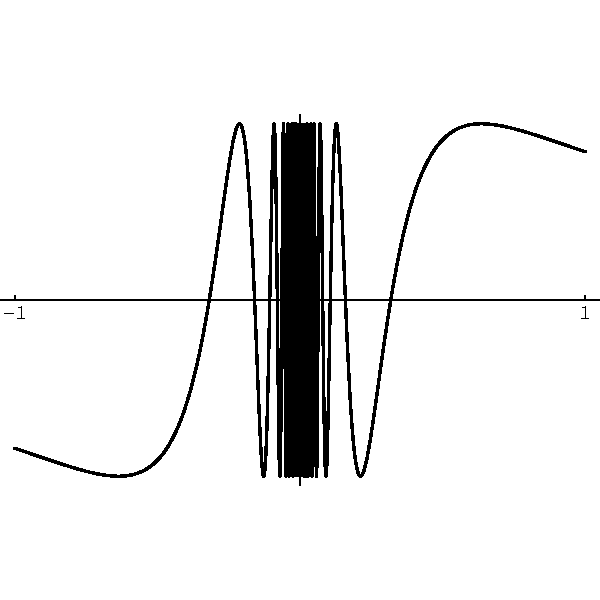
\includegraphics[width=0.6\textwidth]{ode/self_adjoint_bvp/finclust}
  \end{center}
  \caption{Function with a finite cluster point.}
  \label{fin_clust}
\end{figure}









\paragraph{Infinite Number of Eigenvalues.}
Though we will not show it, self-adjoint problems have an infinite number
of eigenvalues. Thus the eigenfunctions form an infinite orthogonal set.







\paragraph{Eigenvalues of Second Order Problems.}
Consider the second order, self-adjoint eigenvalue problem
\[ L[y] = (p y')' + q y = \lambda y, \quad \mathrm{on}\ a \leq x \leq b,
\quad \mathrm{subject to}\ B_j[y] = 0.\]
Let $\lambda_n$ be an eigenvalue with the eigenfunction $\phi_n$.
\begin{gather*}
  \langle \phi_n | L[\phi_n] \rangle = \langle \phi_n | \lambda_n \phi_n \rangle \\
  \langle \phi_n | (p \phi_n')' + q \phi_n \rangle = \lambda_n 
  \langle \phi_n | \phi_n \rangle \\
  \int_a^b \overline{\phi_n} (p \phi_n')'\,\dd x + \langle \phi_n | q | \phi_n\rangle
  = \lambda_n \langle \phi_n | \phi_n \rangle \\
  \big[\overline{\phi_n} p \phi_n'\big]_a^b - \int_a^b \overline{\phi_n}' p \phi_n'\,\dd x
  + \langle \phi_n | q | \phi_n\rangle = \lambda_n \langle \phi_n | \phi_n \rangle \\
  \boxed{ \lambda_n = \frac{[p \overline{\phi_n} \phi_n']_a^b 
      - \langle \phi_n' | p | \phi_n' \rangle + \langle \phi_n | q | \phi_n \rangle}
    { \langle \phi_n | \phi_n \rangle } }
\end{gather*}

Thus we can express each eigenvalue in terms of its eigenfunction.  You
might think that this formula is just a shade less than worthless.  When
solving an eigenvalue problem you have to find the eigenvalues before
you determine the eigenfunctions.  Thus this formula could not be used
to compute the eigenvalues.  However, we can often use the formula to
obtain information about the eigenvalues before we solve a problem.




\begin{Example}
  Consider the self-adjoint eigenvalue problem
  \[ -y'' = \lambda y, \qquad y(0) = y(\pi) = 0.\]
  The eigenvalues are given by the formula
  \begin{align*}
    \lambda_n &= \frac{\big[(-1) \overline{\phi} \phi'\big]_a^b 
      - \langle \phi_n' | (-1) | \phi_n'\rangle
      + \langle \phi_n | 0 | \phi_n \rangle }
    {\langle \phi_n | \phi_n \rangle} \\
    &= \frac{0 + \langle \phi_n' | \phi_n' \rangle + 0}{\langle \phi_n | \phi_n \rangle}.
  \end{align*}
  We see that $\lambda_n \geq 0$.  If $\lambda_n = 0$ then $\langle \phi_n' | \phi_n' \rangle
  = 0$,which implies that $\phi_n = \mathrm{const}$.  The only constant that
  satisfies the boundary conditions is $\phi_n = 0$ which is not an 
  eigenfunction since it is the trivial solution.  Thus the eigenvalues are 
  positive.
\end{Example}













%%============================================================================
\section{Inhomogeneous Equations}



Let the problem,
\[ 
L[y] = 0, \quad B_k[y] = 0,
\]
be self-adjoint.  If the inhomogeneous problem,
\[ 
L[y] = f, \quad B_k[y] = 0,
\]
has a solution, then we we can write this solution in terms of the 
eigenfunction of the associated eigenvalue problem,
\[ 
L[y] = \lambda y, \quad B_k[y] = 0.
\]


We denote the eigenvalues as $\lambda_n$ and the eigenfunctions as $\phi_n$ for 
$n \in \mathbb{Z}^+$.  For the moment we assume that $\lambda = 0$ is not an 
eigenvalue and that the eigenfunctions are real-valued.  We expand the 
function $f(x)$ in a series of the eigenfunctions.
\[
f(x) = \sum f_n \phi_n(x), \quad
f_n = \frac{ \langle \phi_n | f \rangle }{ \| \phi_n \| }
\]
We expand the inhomogeneous solution in a series of eigenfunctions and 
substitute it into the differential equation.
\begin{gather*}
  L[y] = f
  \\
  L \left[ \sum y_n \phi_n(x) \right] = \sum f_n \phi_n(x)
  \\
  \sum \lambda_n y_n \phi_n(x) = \sum f_n \phi_n(x)
  \\
  y_n = \frac{f_n}{\lambda_n}
\end{gather*}
The inhomogeneous solution is
\begin{equation}
  \label{y=sumfnflfnfnfn}
  y(x) = \sum \frac{ \langle \phi_n | f \rangle }{ \lambda_n \| \phi_n \| } \phi_n(x).
\end{equation}

As a special case we consider the Green function problem,
\[ 
L[G] = \delta(x - \xi), \quad B_k[G] = 0,
\]
We expand the Dirac delta function in an eigenfunction series.
\[
\delta(x - \xi) 
= \sum \frac{ \langle \phi_n | \delta \rangle }{ \| \phi_n \| } \phi_n(x)
= \sum \frac{ \phi_n(\xi) \phi_n(x) }{ \| \phi_n \| }
\]
The Green function is
\[
G(x|\xi) = \sum \frac{ \phi_n(\xi) \phi_n(x) }{ \lambda_n \| \phi_n \| }.
\]
We corroborate Equation~\ref{y=sumfnflfnfnfn} by solving the inhomogeneous 
equation in terms of the Green function.
\begin{gather*}
  y = \int_a^b G(x|\xi) f(\xi) \,\dd \xi
  \\
  y = \int_a^b \sum \frac{ \phi_n(\xi) \phi_n(x) }{ \lambda_n \| \phi_n \| } f(\xi) \,\dd \xi
  \\
  y = \sum \frac{ \int_a^b \phi_n(\xi) f(\xi) \,\dd \xi }{ \lambda_n \| \phi_n \| } \phi_n(x) 
  \\
  y = \sum \frac{ \langle \phi_n | f \rangle }{ \lambda_n \| \phi_n \| } \phi_n(x)
\end{gather*}











\begin{Example}
  Consider the Green function problem
  \[
  G'' + G = \delta(x - \xi), \quad G(0|\xi) = G(1|\xi) = 0.
  \]
  First we examine the associated eigenvalue problem.
  \begin{gather*}
    \phi'' + \phi = \lambda \phi, \quad \phi(0) = \phi(1) = 0
    \\
    \phi'' + (1 - \lambda)\phi = 0, \quad \phi(0) = \phi(1) = 0
    \\
    \lambda_n = 1 - (n \pi)^2, \quad \phi_n = \sin(n \pi x), \quad n \in \mathbb{Z}^+
  \end{gather*}
  We write the Green function as a series of the eigenfunctions.
  \[
  G(x|\xi) = 2 \sum_{n = 1}^\infty \frac{ \sin(n \pi \xi) \sin(n \pi x) }{ 1 - (n \pi)^2 }
  \]
\end{Example}










%% CONTINUE HERE
%% Do the \lambda = 0 case.





\raggedbottom
%%============================================================================
\exercises{
\pagebreak
\flushbottom
\section{Exercises}






%%-----------------------------------------------------------------------------
%%\begin{large}
%%\noindent
%%\textbf{}
%%\end{large}






%% L y = y^{(n)} + p_1(z) y^{(n-1)} + p_2(z) y^{(n-2)} + \cdots + p_n(z) y.
\begin{Exercise}
  \label{exercise adjoint operator n}
  Show that the operator adjoint to
  \[
  L y = y^{(n)} + p_1(z) y^{(n-1)} + p_2(z) y^{(n-2)} + \cdots + p_n(z) y
  \]
  is given by
  \[
  M y = (-1)^n u^{(n)} + (-1)^{n-1} (\overline{p_1(z)} u)^{(n-1)} 
  + (-1)^{n-2} (\overline{p_2(z)} u)^{(n-2)} + \cdots + \overline{p_n(z)} u.
  \]

  \hintsolution{adjoint operator n}
\end{Exercise}








\raggedbottom
}
%%============================================================================
\hints{
\pagebreak
\flushbottom
\section{Hints}




%%-----------------------------------------------------------------------------
%%\begin{large}
%%\noindent
%%\textbf{}
%%\end{large}




%% L y = y^{(n)} + p_1(z) y^{(n-1)} + p_2(z) y^{(n-2)} + \cdots + p_n(z) y.
\begin{Hint}
  \label{hint adjoint operator n}
  %% CONTINUE
\end{Hint}








\raggedbottom
}
%%============================================================================
\solutions{
\pagebreak
\flushbottom
\section{Solutions}






%%-----------------------------------------------------------------------------
%%\begin{large}
%%\noindent
%%\textbf{}
%%\end{large}







%% L y = y^{(n)} + p_1(z) y^{(n-1)} + p_2(z) y^{(n-2)} + \cdots + p_n(z) y.
\begin{Solution}
  \label{solution adjoint operator n}
  Consider $u(x), v(x) \in C^n$. ($C^n$ is the set of $n$ times continuously
  differentiable functions). First we prove the preliminary result
  \begin{equation}
    \label{eqn_uvn_unv}
    u v^{(n)} - (-1)^n u^{(n)} v = 
    \frac{\dd}{\dd x} \sum_{k=0}^{n-1} (-1)^k u^{(k)} v^{(n-k-1)}
  \end{equation}
  by simplifying the right side.
  \begin{align*}
    \frac{\dd}{\dd x} \sum_{k=0}^{n-1} (-1)^k u^{(k)} v^{(n-k-1)}
    &= \sum_{k=0}^{n-1} (-1)^k \left( u^{(k)} v^{(n-k)} 
      + u^{(k+1)} v^{(n-k-1)} \right) \\
    &= \sum_{k=0}^{n-1} (-1)^k u^{(k)} v^{(n-k)} 
    - \sum_{k=0}^{n-1} (-1)^{k+1} u^{(k+1)} v^{(n-k-1)} \\
    &= \sum_{k=0}^{n-1} (-1)^k u^{(k)} v^{(n-k)} 
    - \sum_{k=1}^{n} (-1)^{k} u^{(k)} v^{(n-k)} \\
    &= (-1)^0 u^{(0)} v^{n-0} - (-1)^n u^{(n)} v^{(n-n)} \\
    &= u v^{(n)} - (-1)^n u^{(n)} v
  \end{align*}

  We define $p_0(x) = 1$ so that we can write the operators in a nice form.
  \[
  L y = \sum_{m=0}^n p_m(z) y^{(n-m)}, \quad
  M u = \sum_{m=0}^n (-1)^m (\overline{p_m(z)} u)^{(n-m)}
  \]
  Now we show that $M$ is the adjoint to $L$.
  \begin{align*}
    \overline{u} L y - y \overline{M u}
    &= \overline{u} \sum_{m=0}^n p_m(z) y^{(n-m)}
    - y \sum_{m=0}^n (-1)^m (p_m(z) \overline{u})^{(n-m)} \\
    &= \sum_{m=0}^n \left( \overline{u} p_m(z) y^{(n-m)} 
      - (p_m(z) \overline{u})^{(n-m)} y 
    \right) \\
    \intertext{We use Equation~\ref{eqn_uvn_unv}.}
    &= \sum_{m=0}^n \frac{\dd}{\dd z} \sum_{k=0}^{n-m-1} 
    (-1)^k (\overline{u} p_m(z))^{(k)} y^{(n-m-k-1)}
  \end{align*}
  \[
  \boxed{
    \overline{u} L y - y \overline{M u} = \frac{\dd}{\dd z} \sum_{m=0}^n \sum_{k=0}^{n-m-1} 
    (-1)^k (\overline{u} p_m(z))^{(k)} y^{(n-m-k-1)}
    }
  \]
\end{Solution}








\raggedbottom
}


\flushbottom


%% CONTINUE: Fix the d t's
%%
%% Change the scale in Figure 1.1 to units of \pi.
%%
%% Plot the approximation to the function in figure 4.
%%




%%===========================================================================
%%==========================================================================
\chapter{Fourier Series}
\index{Fourier series}

%%CONTINUE: the beginning
%%\ldots to achieve spiritual creaminess and avoid the chunky degradation.

%%\begin{flushright}
%%-Jim Carrey, Ace Ventura 2.
%%\end{flushright}




\begin{tabbing}
  Every time I close my eyes \\
  The noise inside me amplifies \\
  I can't escape \\
  I relive every moment of the day \\
  Every misstep I have made \\
  Finds a way it can invade \\
  My every thought \\
  And this is why I find myself awake
\end{tabbing}

\begin{flushright}
  -\textit{Failure}\\
  -Tom Shear (Assemblage 23)
\end{flushright}






%%===========================================================================
\section{An Eigenvalue Problem.}
\index{eigenvalue problems}
\index{eigenvalues}
\index{eigenfunctions}



\paragraph{A self adjoint eigenvalue problem.}
Consider the eigenvalue problem
\[ 
y'' + \lambda y = 0, \qquad y(-\pi) = y(\pi), \qquad y'(-\pi) = y'(\pi).
\]
We rewrite the equation so the eigenvalue is on the right side.
\[
L[y] \equiv - y'' = \lambda y
\]
We demonstrate that this eigenvalue problem is self adjoint.
\begin{align*}
  \langle v | L[u] \rangle - \langle L[v] | u \rangle 
  &= \langle v | -u'' \rangle - \langle - v'' | u \rangle 
  \\
  &= [ - \bar{v} u' ]_{-\pi}^\pi + \langle v' | u' \rangle - [ - \bar{v}' u ]{-\pi}^\pi - \langle v' | u' \rangle 
  \\
  &= - \overline{v(\pi)} u'(\pi) + \overline{v(-\pi)} u'(-\pi) 
  + \overline{v'(\pi)} u(\pi) - \overline{v'(-\pi)} u(-\pi) 
  \\
  &= - \overline{v(\pi)} u'(\pi) + \overline{v(\pi)} u'(\pi) 
  + \overline{v'(\pi)} u(\pi) - \overline{v'(\pi)} u(\pi) 
  \\
  &= 0
\end{align*}
Since Green's Identity reduces to $\langle v | L[u] \rangle - \langle L[v] | u \rangle = 0$, the 
problem is self adjoint.  This means that the eigenvalues are real 
and that eigenfunctions corresponding to distinct eigenvalues are orthogonal.
We compute the Rayleigh quotient for an eigenvalue $\lambda$ with eigenfunction $\phi$.
\begin{align*}
  \lambda &= \frac{ - [ \bar{\phi} \phi' ]_{-\pi}^\pi + \langle \phi' | \phi' \rangle }{ \langle \phi | \phi \rangle }
  \\
  &= \frac{ - \overline{\phi(\pi)} \phi'(\pi) + \overline{\phi(-\pi)} \phi'(-\pi) 
    + \langle \phi' | \phi' \rangle }{ \langle \phi | \phi \rangle }
  \\
  &= \frac{ - \overline{\phi(\pi)} \phi'(\pi) + \overline{\phi(\pi)} \phi'(\pi) 
    + \langle \phi' | \phi' \rangle }{ \langle \phi | \phi \rangle }
  \\
  &= \frac{ \langle \phi' | \phi' \rangle }{ \langle \phi | \phi \rangle }
\end{align*}
We see that the eigenvalues are non-negative.


\paragraph{Computing the eigenvalues and eigenfunctions.}
Now we find the eigenvalues and eigenfunctions.
First we consider the case $\lambda = 0$.  The general solution of the 
differential equation is
\[ 
y = c_1 + c_2 x.
\]
The solution that satisfies the boundary conditions is $y = \mathrm{const}$.

Now consider $\lambda > 0$.
The general solution of the differential equation is
\[ 
y = c_1 \cos \left( \sqrt{\lambda} x \right) + c_2 \sin \left( \sqrt{\lambda} x \right).
\]
We apply the first boundary condition.
\begin{gather*}
  y(-\pi) = y(\pi) 
  \\
  c_1 \cos \left(-\sqrt{\lambda}\pi \right) + c_2 \sin \left(-\sqrt{\lambda}\pi \right) 
  = c_1 \cos \left(\sqrt{\lambda}\pi \right) + c_2 \sin \left(\sqrt{\lambda}\pi \right) 
  \\
  c_1 \cos \left(\sqrt{\lambda}\pi \right) - c_2 \sin \left(\sqrt{\lambda}\pi \right) 
  = c_1 \cos \left(\sqrt{\lambda}\pi \right) + c_2 \sin \left(\sqrt{\lambda}\pi \right) 
  \\
  c_2 \sin \left(\sqrt{\lambda}\pi \right) = 0
\end{gather*}
Then we apply the second boundary condition.
\begin{gather*}
  y'(-\pi) = y'(\pi) 
  \\
  - c_1 \sqrt{\lambda} \sin \left(-\sqrt{\lambda}\pi \right) 
  + c_2 \sqrt{\lambda} \cos \left(-\sqrt{\lambda}\pi \right) 
  = - c_1 \sqrt{\lambda} \sin \left(\sqrt{\lambda}\pi \right) 
  + c_2 \sqrt{\lambda} \cos \left(\sqrt{\lambda}\pi \right) 
  \\
  c_1 \sin \left(\sqrt{\lambda}\pi \right) 
  + c_2 \cos \left(\sqrt{\lambda}\pi \right) 
  = - c_1 \sin \left(\sqrt{\lambda}\pi \right) 
  + c_2 \cos \left(\sqrt{\lambda}\pi \right) 
  \\
  c_1 \sin \left( \sqrt{\lambda}\pi \right) = 0
\end{gather*}
To satisify the two boundary conditions either $c_1 = c_2 = 0$ or 
$\sin \left( \sqrt{\lambda}\pi \right) = 0$.  The former yields the trivial solution.
The latter gives us the eigenvalues $\lambda_n = n^2$, $n \in \mathbb{Z}^+$.
The corresponding solution is 
\[
y_n = c_1 \cos(n x) + c_2 \sin(n x).
\]
There are two eigenfunctions for each of the positive eigenvalues.

We choose the eigenvalues and eigenfunctions.
\begin{alignat*}{2}
  \lambda_0 &= 0, &\qquad \phi_0 &= \frac{1}{2} 
  \\
  \lambda_n &= n^2, &\qquad \phi_{2n-1} &= \cos(n x), \quad 
  \phi_{2n} = \sin(n x), \quad \mathrm{for}\ n = 1, 2, 3, \ldots
\end{alignat*}


\paragraph{Orthogonality of Eigenfunctions.}
We know that the eigenfunctions of distinct eigenvalues are orthogonal.
In addition, the two eigenfunctions of each positive eigenvalue are 
orthogonal.
\[
\int_{-\pi}^\pi \cos(n x) \sin(n x) \,\dd x
= \left[ \frac{1}{2 n} \sin^2(n x) \right]_{-\pi}^\pi 
= 0
\]
Thus the eigenfunctions 
$\{ \frac{1}{2}, \cos(x), \sin(x), \cos(2 x), \sin(2 x) \}$ are an orthogonal
set.








%%============================================================================
\section{Fourier Series.}





A series of the eigenfunctions
\[
\phi_0 = \frac{1}{2}, \quad \phi_n^{(1)} = \cos(n x), 
\quad \phi_n^{(2)} = \sin(n x), \quad \mathrm{for}\ n \geq 1
\]
is
\[ 
\frac{1}{2} a_0 + \sum_{n=1}^\infty 
\big(a_n \cos(n x) + b_n \sin(n x)\big).
\]
This is known as a \textit{Fourier series}.
(We choose $\phi_0 = \frac{1}{2}$ so all of the eigenfunctions have the same norm.)
A fairly general class of functions can be expanded in Fourier series.  
Let $f(x)$ be a function defined on $-\pi < x < \pi$.
Assume that $f(x)$ can be expanded in a Fourier series
\begin{equation} \label{four_ser}
  f(x) \sim \frac{1}{2} a_0 + \sum_{n=1}^\infty 
  \big(a_n \cos(n x) + b_n \sin(n x)\big).
\end{equation}
Here the ``$\sim$'' means ``has the Fourier series''.  We have not said
if the series converges yet.  For now let's assume that the series 
converges uniformly so we can replace the $\sim$ with an $=$.  

We integrate Equation~\ref{four_ser} from $-\pi$ to $\pi$ to determine $a_0$.
\begin{gather*}
  \int_{-\pi}^\pi f(x)\,\dd x = \frac{1}{2}a_0 \int_{-\pi}^\pi\,\dd x
  + \int_{-\pi}^\pi \sum_{n=1}^\infty a_n \cos(n x) 
  + b_n \sin(n x)\,\dd x\\
  \int_{-\pi}^\pi f(x)\,\dd x = \pi a_0 + \sum_{n=1}^\infty \left(
    a_n \int_{-\pi}^\pi \cos(n x)\,\dd x 
    + b_n \int_{-\pi}^\pi \sin(n x)\,\dd x \right) \\
  \int_{-\pi}^\pi f(x)\,\dd x = \pi a_0 \\
  a_0 = \frac{1}{\pi} \int_{-\pi}^\pi f(x)\,\dd x 
\end{gather*} 

Multiplying by $\cos(m x)$ and integrating will enable us to solve for $a_m$.
\begin{align*}
  \int_{-\pi}^\pi f(x) \cos(m x)\,\dd x &= 
  \frac{1}{2}a_0 \int_{-\pi}^\pi \cos(m x)\,\dd x \\
  &\qquad 
  + \sum_{n=1}^\infty \left(a_n \int_{-\pi}^\pi \cos(n x) \cos(m x)\,\dd x
    + b_n \int_{-\pi}^\pi \sin(n x) \cos(m x)\,\dd x \right) 
\end{align*}
All but one of the terms on the right side vanishes due to the 
orthogonality of the eigenfunctions.
\begin{gather*}
  \int_{-\pi}^\pi f(x) \cos(m x)\,\dd x = 
  a_m \int_{-\pi}^\pi \cos(m x) \cos(m x)\,\dd x \\
  \int_{-\pi}^\pi f(x) \cos(m x)\,\dd x = a_m \int_{-\pi}^\pi \left( \frac{1}{2}
    + \cos(2m x) \right)\,\dd x \\
  \int_{-\pi}^\pi f(x) \cos(m x)\,\dd x = \pi a_m \\
  a_m = \frac{1}{\pi} \int_{-\pi}^\pi f(x) \cos(m x)\,\dd x.
\end{gather*}
Note that this formula is valid for $m = 0, 1, 2, \ldots$.

Similarly, we can multiply by $\sin(m x)$ and integrate to solve for $b_m$.
The result is
\[ 
b_m = \frac{1}{\pi} \int_{-\pi}^\pi f(x) \sin(m x)\,\dd x. 
\]
$a_n$ and $b_n$ are called \textit{Fourier coefficients}.
\index{Fourier coefficients}



Although we will not show it, Fourier series converge for a 
fairly general class of functions.
Let $f(x^-)$ denote the left limit of $f(x)$ and $f(x^+)$ denote the right
limit.




\begin{Example}
  For the function defined
  \[ f(x) = 
  \begin{cases}
    0 \quad &\mathrm{for}\ x < 0, \\
    x + 1 \quad &\mathrm{for}\ x \geq 0,
  \end{cases}
  \]
  the left and right limits at $x = 0$ are
  \[ f(0^-) = 0, \qquad f(0^+) = 1.\]
\end{Example}








\begin{Result}
  Let $f(x)$ be a $2\pi$-periodic function for which $\int_{-\pi}^\pi
  |f(x)|\,\dd x$ exists.  Define the Fourier coefficients
  \[ 
  a_n = \frac{1}{\pi} \int_{-\pi}^\pi f(x) \cos(n x)\,\dd x, \qquad
  b_n = \frac{1}{\pi} \int_{-\pi}^\pi f(x) \sin(n x)\,\dd x. 
  \] 
  If $x$ is an interior point of an interval on which $f(x)$ has limited
  total fluctuation, then the Fourier series of $f(x)$
  \[ 
  \frac{a_0}{2} + \sum_{n=1}^\infty \big(a_n \cos(n x) + b_n \sin(n x) \big),
  \]
  converges to $\frac{1}{2} (f(x^-) + f(x^+))$.  If $f$ is continuous at
  $x$, then the series converges to $f(x)$.
\end{Result}






\paragraph{Periodic Extension of a Function.}
\index{periodic extension}
Let $g(x)$ be a function that is arbitrarily defined on $-\pi \leq x < \pi$.
The Fourier series of $g(x)$ will represent the periodic extension of $g(x)$.
The periodic extension, $f(x)$, is defined by the two conditions:
\begin{gather*}
  f(x) = g(x) \quad \mathrm{for}\ -\pi \leq x < \pi, \\
  f(x + 2\pi) = f(x).
\end{gather*}

The periodic extension of $g(x) = x^2$ is shown in Figure~\ref{per_ext_xs}.

\begin{figure}[h!]
  \begin{center}
    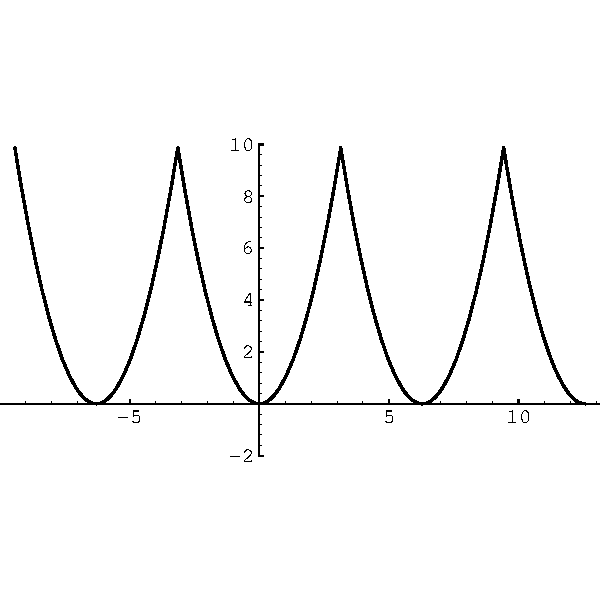
\includegraphics[width=0.6\textwidth]{ode/fourier_series/per_ext}
  \end{center}
  \caption{The periodic extension.}
  \label{per_ext_xs}
\end{figure}


\paragraph{Limited Fluctuation.}
A function that has limited total fluctuation can be written $f(x) = \psi_+(x) - \psi_-(x)$,
where $\psi_+$ and $\psi_-$ are bounded, nondecreasing functions.
An example of a function that does not have limited total fluctuation
is $\sin(1/x)$, whose fluctuation is unlimited at the point $x=0$.

\paragraph{Functions with Jump Discontinuities.}
\index{discontinuous functions}
Let $f(x)$ be a discontinuous function that has a convergent Fourier 
series.  Note that the series does not necessarily converge to $f(x)$.
Instead it converges to $\hat{f}(x) = \frac{1}{2}(f(x^-)+f(x^+))$.


\begin{Example}
  Consider the function defined by
  \[ f(x) = 
  \begin{cases}
    -x \quad &\mathrm{for}\ -\pi \leq x < 0 \\
    \pi - 2x \quad &\mathrm{for}\ 0 \leq x < \pi.
  \end{cases}
  \]
  The Fourier series converges to the function defined by
  \[ \hat{f}(x) = 
  \begin{cases}
    0 \quad &\mathrm{for}\ x = -\pi \\
    -x \quad &\mathrm{for}\ -\pi < x < 0 \\
    \pi / 2 \quad &\mathrm{for}\ x = 0 \\
    \pi - 2x \quad &\mathrm{for}\ 0 < x < \pi. 
  \end{cases}
  \]
  The function $\hat{f}(x)$ is plotted in Figure~\ref{disc_fcn}.

  \begin{figure}[h!]
    \begin{center}
      \includegraphics[width=0.6\textwidth]{ode/fourier_series/disc_fcn}
    \end{center}
    \caption{The function to which the Fourier series converges.}
    \label{disc_fcn}
  \end{figure}

\end{Example}











%%==========================================================================
\section{Least Squares Fit}
\index{least squares fit!Fourier series}



\paragraph{Approximating a function with a Fourier series.}
Suppose we want to approximate a $2\pi$-periodic function $f(x)$ with
a finite Fourier series.
\[ 
f(x) \approx \frac{a_0}{2} + \sum_{n=1}^{N} (a_n \cos(n x) + b_n \sin(n x))
\]
Here the coefficients are computed with the familiar formulas.
Is this the best approximation to the function?  That is, is it possible
to choose coefficients $\alpha_n$ and $\beta_n$ such that
\[ 
f(x) \approx \frac{\alpha_0}{2} + \sum_{n=1}^N (\alpha_n \cos(n x) + \beta_n \sin(n x)) 
\]
would give a better approximation?



\paragraph{Least squared error fit.}
The most common criterion for finding the best fit to a function is the
least squares fit.  The best approximation to a function is defined
as the one that minimizes the integral of the square of the deviation.
Thus if $f(x)$ is to be approximated on the interval $a \leq x \leq b$
by a series
\begin{equation}
  \label{eqn f = sum cn phin}
  f(x) \approx \sum_{n=1}^{N} c_n \phi_n(x),
\end{equation}
the best approximation is found by choosing values of $c_n$ that
minimize the error $E$.
\[ 
E \equiv \int_a^b \left| f(x) - \sum_{n=1}^{N} c_n \phi_n(x) \right|^2\,\dd x
\]


\paragraph{Generalized Fourier coefficients.}
We consider the case that the $\phi_n$ are orthogonal.  
For simplicity, we also assume that the $\phi_n$ are real-valued.
Then most of the terms
will vanish when we interchange the order of integration and summation.
\begin{gather*}
  E = \int_a^b \left( f^2 - 2 f \sum_{n=1}^{N} c_n \phi_n 
    + \sum_{n=1}^{N} c_n \phi_n \sum_{m=1}^{N} c_m \phi_m \right)\,\dd x
  \\
  E = \int_a^b f^2 \,\dd x - 2 \sum_{n=1}^{N} c_n \int_a^b f \phi_n \,\dd x
  + \sum_{n=1}^{N} \sum_{m=1}^{N} c_n c_m \int_a^b \phi_n \phi_m \,\dd x
  \\
  E = \int_a^b f^2 \,\dd x - 2 \sum_{n=1}^{N} c_n \int_a^b f \phi_n \,\dd x
  + \sum_{n=1}^{N} c_n^2 \int_a^b \phi_n^2 \,\dd x
  \\
  E = \int_a^b f^2 \,\dd x 
  + \sum_{n=1}^{N} \left( c_n^2 \int_a^b \phi_n^2 \,\dd x - 2 c_n \int_a^b f \phi_n \,\dd x \right)
  \\
  \intertext{We complete the square for each term.}
  E = \int_a^b f^2 \,\dd x 
  + \sum_{n=1}^{N} \left( \int_a^b \phi_n^2 \,\dd x \left( c_n 
      - \frac{ \int_a^b f \phi_n \,\dd x}{\int_a^b \phi_n^2 \,\dd x } \right)^2
    - \left( \frac{ \int_a^b f \phi_n \,\dd x}{\int_a^b \phi_n^2 \,\dd x } \right)^2 \right)
\end{gather*}
Each term involving $c_n$ is non-negative, and is minimized for
\begin{equation}
  \label{eqn cn = frac int f phi int phi2}
  c_n = \frac{ \int_a^b f \phi_n \,\dd x}{\int_a^b \phi_n^2 \,\dd x }.
\end{equation}
We call these the \textit{generalized Fourier coefficients}.

For such a choice of the $c_n$, the error is
\[
E = \int_a^b f^2 \,\dd x - \sum_{n=1}^{N} c_n^2 \int_a^b \phi_n^2 \,\dd x.
\]
Since the error is non-negative, we have
\[
\int_a^b f^2 \,\dd x \geq \sum_{n=1}^{N} c_n^2 \int_a^b \phi_n^2 \,\dd x.
\]
This is known as \textit{Bessel's Inequality}.
\index{Bessel's inequality}
If the series in Equation~\ref{eqn f = sum cn phin} converges in the mean
to $f(x)$, $\lim{N \to \infty} E = 0$, then we have equality as $N \to \infty$.
\[
\int_a^b f^2 \,\dd x = \sum_{n=1}^\infty c_n^2 \int_a^b \phi_n^2 \,\dd x.
\]
This is \textit{Parseval's equality}.
\index{Parseval's equality}




\paragraph{Fourier coefficients.}
Previously we showed that if the series,
\[ 
f(x) = \frac{a_0}{2} + \sum_{n=1}^\infty (a_n \cos(n x) + b_n \sin(n x),
\]
converges uniformly then the coefficients in the series are the Fourier 
coefficients,
\[ 
a_n = \frac{1}{\pi} \int_{-\pi}^\pi f(x) \cos(n x)\,\dd x, \qquad
b_n = \frac{1}{\pi} \int_{-\pi}^\pi f(x) \sin(n x)\,\dd x. 
\]
Now we show that by choosing the coefficients to minimize the squared error,
we obtain the same result.
We apply Equation~\ref{eqn cn = frac int f phi int phi2} to the Fourier
eigenfunctions.
\begin{gather*}
  a_0 = \frac{ \int_{-\pi}^\pi f \frac{1}{2} \,\dd x }{ \int_{-\pi}^\pi \frac{1}{4} \,\dd x }
  = \frac{1}{\pi} \int_{-\pi}^\pi f(x)\,\dd x
  \\
  a_n = \frac{ \int_{-\pi}^\pi f \cos(n x) \,\dd x }{ \int_{-\pi}^\pi \cos^2(n x) \,\dd x }
  = \frac{1}{\pi} \int_{-\pi}^\pi f(x) \cos(n x)\,\dd x
  \\
  b_n = \frac{ \int_{-\pi}^\pi f \sin(n x) \,\dd x }{ \int_{-\pi}^\pi \sin^2(n x) \,\dd x }
  = \frac{1}{\pi} \int_{-\pi}^\pi f(x) \sin(n x)\,\dd x
\end{gather*}













%%==========================================================================
\section{Fourier Series for Functions Defined on Arbitrary Ranges}






If $f(x)$ is defined on $c-d \leq x < c+d$ and $f(x + 2d) = f(x)$, then
$f(x)$ has a Fourier series of the form
\[ f(x) \sim \frac{a_0}{2} + \sum_{n=1}^\infty 
a_n \cos\left( \frac{n \pi (x+c)}{d} \right)
+ b_n \sin \left( \frac{n \pi (x+c)}{d} \right) . \]
Since
\[ \int_{c-d}^{c+d} \cos^2 \left( \frac{n \pi (x+c)}{d} \right)\,\dd x = 
\int_{c-d}^{c+d} \sin^2 \left( \frac{n \pi (x+c)}{d} \right)\,\dd x = d,\] 
the Fourier coefficients are given by the formulas
\begin{align*}
  a_n &= \frac{1}{d} \int_{c-d}^{c+d} f(x) \cos \left(
    \frac{n \pi (x+c)}{d} \right)\,\dd x \\
  b_n &= \frac{1}{d} \int_{c-d}^{c+d} f(x) \sin \left(
    \frac{n \pi (x+c)}{d} \right)\,\dd x. 
\end{align*}





\begin{Example}
  Consider the function defined by
  \[ f(x) =       \begin{cases}
    x+1 \quad &\mathrm{for}\ -1 \leq x < 0 \\
    x \quad &\mathrm{for}\ 0 \leq x < 1 \\
    3-2x \quad &\mathrm{for}\ 1 \leq x < 2.
  \end{cases}
  \]
  This function is graphed in Figure~\ref{uud12}.



  The Fourier series converges to $\hat{f}(x) = (f(x^-) + f(x^+))/2$, 
  \[ \hat{f}(x) = 
  \begin{cases}
    -\frac{1}{2} \quad &\mathrm{for}\ x = -1 \\
    x+1 \quad &\mathrm{for}\ -1 < x < 0 \\
    \frac{1}{2} \quad &\mathrm{for}\ x = 0 \\
    x \quad &\mathrm{for}\ 0 < x < 1 \\
    3-2x \quad &\mathrm{for}\ 1 \leq x < 2.
  \end{cases}
  \]
  $\hat{f}(x)$ is also graphed in Figure~\ref{uud12}.


  \begin{figure}[h!]
    \begin{center}
      \includegraphics[width=0.49\textwidth]{ode/fourier_series/uud1}
      \includegraphics[width=0.49\textwidth]{ode/fourier_series/uud2}
    \end{center}
    \caption{A function defined on an interval and 
      the function to which the Fourier series converges.}
    \label{uud12}
  \end{figure}


  The Fourier coefficients are
  \begin{align*}
    a_n &= \frac{1}{3/2} \int_{-1}^2 f(x) \cos \left( \frac{2 n \pi (x+1/2)}{3}
    \right)\,\dd x \\
    &= \frac{2}{3} \int_{-1/2}^{5/2} f(x-1/2) \cos \left(
      \frac{2 n \pi x}{3} \right)\,\dd x \\
    &= \frac{2}{3} \int_{-1/2}^{1/2} (x + 1/2) \cos \left(
      \frac{2 n \pi x}{3} \right)\,\dd x 
    + \frac{2}{3} \int_{1/2}^{3/2} (x - 1/2) \cos \left(
      \frac{2 n \pi x}{3} \right)\,\dd x \\
    &\qquad \qquad+ \frac{2}{3} \int_{3/2}^{5/2} (4 - 2x) \cos \left(
      \frac{2 n \pi x}{3} \right)\,\dd x \\
    &= -\frac{1}{(n\pi)^2}\sin\left( \frac{2n\pi}{3} \right)
    \left[ 2 (-1)^n n \pi + 
      9 \sin\left(\frac{n\pi}{3}\right) \right] 
  \end{align*}
  \begin{align*}
    b_n     &= \frac{1}{3/2} \int_{-1}^2 f(x) \sin \left( \frac{2 n \pi (x+1/2)}{3}
    \right)\,\dd x \\
    &= \frac{2}{3} \int_{-1/2}^{5/2} f(x-1/2) \sin \left(
      \frac{2 n \pi x}{3} \right)\,\dd x \\
    &= \frac{2}{3} \int_{-1/2}^{1/2} (x + 1/2) \sin \left(
      \frac{2 n \pi x}{3} \right)\,\dd x 
    + \frac{2}{3} \int_{1/2}^{3/2} (x - 1/2) \sin \left(
      \frac{2 n \pi x}{3} \right)\,\dd x \\
    &\qquad \qquad + \frac{2}{3} \int_{3/2}^{5/2} (4 - 2x) \sin \left(
      \frac{2 n \pi x}{3} \right)\,\dd x \\
    &= -\frac{2}{(n\pi)^2} \sin^2\left( \frac{n\pi}{3} \right)
    \left[ 2 (-1)^n n \pi + 4 n \pi \cos\left(\frac{n\pi}{3}
      \right) - 3 \sin\left(\frac{n\pi}{3}\right) \right]
  \end{align*}


\end{Example}




%%==========================================================================
\section{Fourier Cosine Series}
\index{Fourier cosine series}

If $f(x)$ is an even function, ($f(-x) = f(x)$), then there will not be 
any sine terms in the Fourier series for $f(x)$.  The Fourier sine 
coefficient is 
\[ b_n = \frac{1}{\pi} \int_{-\pi}^\pi f(x) \sin(n x)\,\dd x.\]
Since $f(x)$ is an even function and $\sin(n x)$ is odd, $f(x) \sin(n x)$ 
is odd.  $b_n$ is the integral of an odd function from $-\pi$ to $\pi$
and is thus zero.  We can rewrite the cosine coefficients,
\begin{align*}
  a_n     &= \frac{1}{\pi} \int_{-\pi}^\pi f(x) \cos(n x)\,\dd x \\
  &= \frac{2}{\pi} \int_0^\pi f(x) \cos(n x)\,\dd x.
\end{align*}




\begin{Example}
  Consider the function defined on $[0, \pi)$ by
  \[ f(x) = 
  \begin{cases}
    x \quad &\mathrm{for}\ 0 \leq x < \pi/2 \\
    \pi - x \quad &\mathrm{for}\ \pi/2 \leq x < \pi.
  \end{cases}
  \]
  The Fourier cosine coefficients for this function are
  \begin{align*}
    a_n     &= \frac{2}{\pi} \int_0^{\pi/2} x \cos(n x)\,\dd x
    + \frac{2}{\pi} \int_{\pi/2}^\pi (\pi - x)\cos(n x)\,\dd x \\
    &=      \begin{cases}
      \frac{\pi}{4} \quad &\mathrm{for}\ n = 0, \\
      \frac{8}{\pi n^2} \cos\left(\frac{n\pi}{2}\right)
      \sin^2\left(\frac{n\pi}{4}\right)
      \quad &\mathrm{for}\ n \geq 1.
    \end{cases}
  \end{align*}
  In Figure~\ref{cos_hill_5} the even periodic extension of $f(x)$ is
  plotted in a dashed line and the sum of the first five nonzero
  terms in the Fourier cosine series are plotted in a solid line.

  \begin{figure}[h!]
    \begin{center}
      \includegraphics[width=0.6\textwidth]{ode/fourier_series/cos_h5}
    \end{center}
    \caption{Fourier Cosine series.}
    \label{cos_hill_5}
  \end{figure}
  
\end{Example}














%%==========================================================================
\section{Fourier Sine Series}
\index{Fourier Sine series}

If $f(x)$ is an odd function, ($f(-x) = - f(x)$), then there will not be any
cosine terms in the Fourier series.  Since $f(x) \cos(n x)$ is an 
odd function, the cosine coefficients will be zero.
Since $f(x) \sin(n x)$ is an even function,we can rewrite the sine coefficients
\[ b_n = \frac{2}{\pi} \int_0^\pi f(x) \sin(n x)\,\dd x.\]




\begin{Example}
  Consider the function defined on $[0, \pi)$ by
  \[ f(x) = 
  \begin{cases}
    x \quad &\mathrm{for}\ 0 \leq x < \pi/2 \\
    \pi - x \quad &\mathrm{for}\ \pi/2 \leq x < \pi.
  \end{cases}
  \]
  The Fourier sine coefficients for this function are
  \begin{align*}
    b_n     &= \frac{2}{\pi} \int_0^{\pi/2} x \sin(n x)\,\dd x
    + \frac{2}{\pi} \int_{\pi/2}^\pi (\pi - x)\sin(n x)\,\dd x \\
    &= \frac{16}{\pi n^2} \cos\left( \frac{n \pi}{4} \right)
    \sin^3\left(\frac{n \pi}{4}\right)             
  \end{align*}
  In Figure~\ref{sin_hill_5} the odd periodic extension of $f(x)$ is
  plotted in a dashed line and the sum of the first five nonzero
  terms in the Fourier sine series are plotted in a solid line.

  \begin{figure}[h!]
    \begin{center}
      \includegraphics[width=0.6\textwidth]{ode/fourier_series/sin_h5}
    \end{center}
    \caption{Fourier Sine series.}
    \label{sin_hill_5}
  \end{figure}

\end{Example}









%%==========================================================================
\section{Complex Fourier Series and Parseval's Theorem}

By writing $\sin(n x)$ and $\cos(n x)$ in terms of $\e^{\imath n x}$ and
$\e^{-\imath n x}$ we can obtain the complex form for a Fourier series.
\begin{align*}
  \frac{a_0}{2} + \sum_{n=1}^\infty \big(a_n \cos(n x) + b_n \sin(n x)\big)
  &= \frac{a_0}{2} + \sum_{n=1}^\infty \left(a_n \frac{1}{2}(\e^{\imath n x}
    + \e^{-\imath n x}) + b_n \frac{1}{\imath 2}(\e^{\imath n x} - \e^{-\imath n x})
  \right)\\
  &= \frac{a_0}{2} + \sum_{n=1}^\infty \left(
    \frac{1}{2}(a_n - \imath b_n) \e^{\imath n x}
    + \frac{1}{2}(a_n + \imath b_n) \e^{-\imath n x} \right) \\
  &= \sum_{n=-\infty}^\infty c_n \e^{\imath n x}
\end{align*}
where
\[ c_n = 
\begin{cases}
  \frac{1}{2}(a_n - \imath b_n) \quad &\mathrm{for}\ n \geq 1 \\
  \frac{a_0}{2} \quad &\mathrm{for}\ n = 0 \\
  \frac{1}{2}(a_{-n} + \imath b_{-n}) \quad &\mathrm{for}\ n \leq -1.
\end{cases}
\]


The functions $\{ \ldots, \e^{-\imath x}, 1, \e^{\imath x}, \e^{\imath 2 x}, \ldots \}$,
satisfy the relation
\begin{align*}
  \int_{-\pi}^\pi \e^{\imath n x} \e^{-\imath m x}\,\dd x 
  &= \int_{-\pi}^\pi \e^{\imath (n-m) x}\,\dd x \\
  &= 
  \begin{cases}
    2 \pi \quad &\mathrm{for}\ n = m \\
    0 \quad &\mathrm{for}\ n \neq m.
  \end{cases}
\end{align*}

Starting with the complex form of the Fourier series of a function $f(x)$,
\[ f(x) \sim \sum_{-\infty}^\infty c_n \e^{\imath n x},\]
we multiply by $\e^{-\imath m x}$ and integrate from $-\pi$ to $\pi$ to obtain
\begin{gather*}
  \int_{-\pi}^\pi f(x) \e^{-\imath m x}\,\dd x = \int_{-\pi}^\pi 
  \sum_{-\infty}^\infty c_n \e^{\imath n x} \e^{-\imath m x}\,\dd x \\
  c_m = \frac{1}{2\pi} \int_{-\pi}^\pi f(x) \e^{-\imath m x}\,\dd x
\end{gather*}

If $f(x)$ is real-valued then
\[ c_{-m} = \frac{1}{2\pi} \int_{-\pi}^\pi f(x) \e^{\imath m x}\,\dd x
= \frac{1}{2\pi} \int_{-\pi}^\pi f(x) \overline{(\e^{-\imath m x})}\,\dd x
= \overline{c_m} \]
where $\bar{z}$ denotes the complex conjugate of $z$.

Assume that $f(x)$ has a uniformly convergent Fourier series.
\begin{align*}
  \int_{-\pi}^\pi f^2(x)\,\dd x
  &= \int_{-\pi}^\pi \left( \sum_{m = -\infty}^\infty c_m \e^{\imath m x}\right)
  \left( \sum_{n = -\infty}^\infty c_n \e^{\imath n x} \right)\,\dd x \\
  &= 2\pi \sum_{n = -\infty}^\infty c_n c_{-n} \\
  &= 2\pi \left( \sum_{n = -\infty}^{-1} \left[ \frac{1}{4}
      (a_{-n} + \imath b_{-n})(a_{-n} - \imath b_{-n}) \right]
    + \frac{a_0}{2} \frac{a_0}{2}
    + \sum_{n=1}^\infty \left[ \frac{1}{4} (a_n - \imath b_n)
      (a_n + \imath b_n) \right] \right) \\
  &= 2 \pi \left( \frac{a_0^2}{4} + \frac{1}{2} 
    \sum_{n=1}^\infty (a_n^2 + b_n^2) \right)
\end{align*}
This yields a result known as Parseval's theorem which holds even when
the Fourier series of
$f(x)$ is not uniformly convergent.



\begin{Result}
  \textbf{Parseval's Theorem. }
  If $f(x)$ has the Fourier series
  \[ f(x) \sim \frac{a_0}{2} + \sum_{n = 1}^\infty (a_n \cos(n x) + b_n \sin(n x)),\]
  then
  \[ \int_{-\pi}^\pi f^2(x)\,\dd x = \frac{\pi}{2} a_0^2
  + \pi \sum_{n = 1}^\infty (a_n^2 + b_n^2).\]
\end{Result}








%%==========================================================================
\section{Behavior of Fourier Coefficients}
\index{Fourier coefficients!behavior of}

Before we jump hip-deep into the grunge involved in determining the
behavior of the Fourier coefficients, let's take a step back and get
some perspective on what we should be looking for.  

One of the important questions is whether the Fourier series converges 
uniformly.  From Result~\ref{unif_cont} we know that a uniformly convergent
series represents a continuous function.  Thus we know that the Fourier
series of a discontinuous function cannot be uniformly convergent.
From Section~\ref{sec_unif_conv} we know that a series is uniformly
convergent if it can be bounded by a series of positive terms.  If the 
Fourier coefficients, $a_n$ and $b_n$, are $O(1/n^\alpha)$ where $\alpha>1$
then the series can be bounded by $(\mathrm{const}) \sum_{n=1}^\infty 1/n^\alpha$
and will thus be uniformly convergent. 









Let $f(x)$ be a function that meets the conditions for having a Fourier 
series and in addition is bounded.  Let $(-\pi, p_1), (p_1, p_2), (p_2, p_3),
\ldots, (p_m, \pi)$ be a partition into a finite number of intervals of the
domain, $(-\pi, \pi)$ such that on each interval $f(x)$ and all its 
derivatives are continuous.  Let $f(p^-)$ denote the left limit of $f(p)$ and 
$f(p^+)$ denote the right limit.
\[
f(p^-) = \lim_{\epsilon \to 0^+} f(p - \epsilon), \qquad
f(p^+) = \lim_{\epsilon \to 0^+} f(p + \epsilon)
\]


\begin{Example}
  The function shown in Figure~\ref{partition} would be partitioned
  into the intervals 
  \[
  (-2, -1), (-1, 0), (0, 1), (1, 2).
  \]

  \begin{figure}[h!]
    \begin{center}
      \includegraphics[width=0.6\textwidth]{ode/fourier_series/partit}
    \end{center}
    \caption{A function that can be partitioned.}
    \label{partition}
  \end{figure}

\end{Example}





Suppose $f(x)$ has the Fourier series
\[ f(x) \sim \frac{a_0}{2} + \sum_{n=1}^\infty a_n \cos(n x) + b_n \sin(n x).\]
We can use the integral formula to find the $a_n$'s.
\begin{align*}
  a_n     &= \frac{1}{\pi} \int_{-\pi}^\pi f(x) \cos(n x)\,\dd x \\
  &= \frac{1}{\pi} \left( \int_{-\pi}^{p_1} f(x) \cos(n x)\,\dd x
    + \int_{p_1}^{p_2} f(x) \cos(n x)\,\dd x + \cdots
    + \int_{p_m}^{\pi} f(x) \cos(n x)\,\dd x \right) \\
  \intertext{Using integration by parts,}
  &= \frac{1}{n\pi} \left(\Big[f(x) \sin(n x)\Big]_{-\pi}^{p_1}
    + \Big[f(x) \sin(n x)\Big]_{p_1}^{p_2} + \cdots
    + \Big[f(x) \sin(n x)\Big]_{p_m}^{\pi} \right) \\
  & \qquad \qquad - \frac{1}{n\pi} \left( \int_{-\pi}^{p_1} f'(x)\sin(n x)\,\dd x
    + \int_{p_1}^{p_2} f'(x)\sin(n x)\,\dd x
    +\int_{p_m}^{\pi} f'(x)\sin(n x)\,\dd x \right) \\
  &= \frac{1}{n\pi} \Big\{ \big[f(p_1^-)-f(p_1^+)\big]\sin(n p_1)
  + \cdots + \big[f(p_m^-)-f(p_m^+)\big]\sin(n p_m) \Big\} \\
  &\qquad \qquad - \frac{1}{n} \frac{1}{\pi} 
  \int_{-\pi}^\pi f'(x)\sin(n x)\,\dd x \\
  &= \frac{1}{n} A_n - \frac{1}{n} b_n'
\end{align*}
where 
\[ A_n = \frac{1}{\pi} \sum_{j=1}^m \sin(n p_j) 
\big[f(p_j^-) - f(p_j^+)\big] \]
and the $b_n'$ are the sine coefficients of $f'(x)$.

Since $f(x)$ is bounded, $A_n = O(1)$.  Since $f'(x)$ is bounded,
\[ b_n' = \frac{1}{\pi} \int_{-\pi}^\pi f'(x) \sin(n x)\,\dd x = O(1).\]
Thus $a_n = O(1/n)$ as $n \to \infty$.
(Actually, from the Riemann-Lebesgue Lemma, $b_n' = \mathcal{O}(1/n)$.)

Now we repeat this analysis for the sine coefficients.
\begin{align*}
  b_n     &= \frac{1}{\pi} \int_{-\pi}^\pi f(x) \sin(n x)\,\dd x \\
  &= \frac{1}{\pi} \left( \int_{-\pi}^{p_1} f(x) \sin(n x)\,\dd x
    + \int_{p_1}^{p_2} f(x) \sin(n x)\,\dd x + \cdots
    + \int_{p_m}^{\pi} f(x) \sin(n x)\,\dd x \right) \\
  &= \frac{-1}{n\pi} \Big\{\big[f(x) \cos(n x)\big]_{-\pi}^{p_1}
  + \big[f(x) \cos(n x)\big]_{p_1}^{p_2} + \cdots
  + \big[f(x) \cos(n x)\big]_{p_m}^{\pi} \Big\} \\
  & \qquad \qquad + \frac{1}{n\pi} \left( \int_{-\pi}^{p_1} f'(x)\cos(n x)\,\dd x
    + \int_{p_1}^{p_2} f'(x)\cos(n x)\,\dd x
    +\int_{p_m}^{\pi} f'(x)\cos(n x)\,\dd x \right) \\
  &= -\frac{1}{n} B_n + \frac{1}{n} a_n'
\end{align*}
where
\[ B_n = \frac{(-1)^n}{\pi} \big[f(-\pi) - f(\pi)\big] 
- \frac{1}{\pi} \sum_{j=1}^m \cos(n p_j)
\big[f(p_j^-) - f(p_j^+)\big] \]
and the $a_n'$ are the cosine coefficients of $f'(x)$.

Since $f(x)$ and $f'(x)$ are bounded, $B_n, a_n' = O(1)$ and thus
$b_n = O(1/n)$ as $n \to \infty$.

With integration by parts on the Fourier coefficients of $f'(x)$ we could
find that
\[ a_n' = \frac{1}{n} A_n' - \frac{1}{n} b_n'' \]
where $A_n' = \frac{1}{\pi} \sum_{j=1}^m \sin(n p_j)[f'(p_j^-)-f'(p_j^+)]$ and
the $b_n''$ are the sine coefficients of $f''(x)$, and
\[ b_n' = -\frac{1}{n} B_n' + \frac{1}{n} a_n'' \]
where $B_n' = \frac{(-1)^n}{\pi} [f'(-\pi) - f'(\pi)] - \frac{1}{\pi} 
\sum_{j=1}^m \cos(n p_j)
[f'(p_j^-)-f'(p_j^+)]$ and the $a_n''$ are the cosine coefficients of $f''(x)$.

Now we can rewrite $a_n$ and $b_n$ as
\begin{align*}
  a_n &= \frac{1}{n} A_n + \frac{1}{n^2} B_n' - \frac{1}{n^2} a_n'' \\
  b_n &= -\frac{1}{n} B_n + \frac{1}{n^2} A_n' - \frac{1}{n^2} b_n''.
\end{align*}

Continuing this process we could define $A_n^{(j)}$ and $B_n^{(j)}$ so that
\begin{align*}
  a_n &= \frac{1}{n} A_n + \frac{1}{n^2} B_n' - \frac{1}{n^3} A_n''
  - \frac{1}{n^4} B_n''' + \cdots \\
  b_n &= -\frac{1}{n} B_n + \frac{1}{n^2} A_n' + \frac{1}{n^3} B_n''
  - \frac{1}{n^4} A_n''' - \cdots. 
\end{align*} 




For any bounded function, the Fourier coefficients satisfy
$a_n, b_n = O(1/n)$ as $n \to \infty$.  If $A_n$ and $B_n$ are zero then the
Fourier coefficients will be $O(1/n^2)$.  A sufficient condition for this
is that the periodic extension of $f(x)$ is continuous. We see
that if the periodic extension of $f'(x)$ is continuous then $A_n'$ and 
$B_n'$ will be zero and the Fourier coefficients will be $O(1/n^3)$.


\begin{Result}
  Let $f(x)$ be a bounded function for which there is a partition of the 
  range $(-\pi, \pi)$ into a finite number of intervals such that $f(x)$ 
  and all its derivatives are continuous on each of the intervals.
  If $f(x)$ is not continuous then the Fourier coefficients are $O(1/n)$.
  If $f(x), f'(x), \ldots, f^{(k-2)}(x)$ are continuous then the Fourier
  coefficients are $O(1/n^k)$.
\end{Result}


If the periodic extension of $f(x)$ is continuous, then the Fourier 
coefficients will be $O(1/n^2)$.  The series 
$\sum_{n=1}^\infty |a_n \cos(n x) b_n \sin(n x)|$ can be bounded by
$M \sum_{n=1}^\infty 1/n^2$ where $M = { \displaystyle \max_{n} }
(|a_n| + |b_n|)$.  Thus 
the Fourier series converges to $f(x)$ uniformly.


\begin{Result}
  If the periodic extension of $f(x)$ is continuous then the Fourier
  series of $f(x)$ will converge uniformly for all $x$.
\end{Result}
\index{uniform convergence!of Fourier series}
\index{Fourier series!uniform convergence}



If the periodic extension of $f(x)$ is not continuous, we have the 
following result.

\begin{Result}
  If $f(x)$ is continuous in the interval $c < x < d$, then the Fourier
  series is uniformly convergent in the interval $c + \delta \leq x \leq
  d - \delta$ for any $\delta > 0$.
\end{Result}








\begin{Example}\textbf{Different Rates of Convergence.}

  \paragraph{A Discontinuous Function.}
  Consider the function defined by
  \[ f_1(x) = 
  \begin{cases}
    -1 \quad &\mathrm{for}\ -1 < x < 0 \\
    1, \quad &\mathrm{for}\ 0 < x < 1.
  \end{cases}
  \]
  This function has jump discontinuities, so we know that the Fourier
  coefficients are $O(1/n)$. 

  Since this function is odd, there will only be sine terms in its Fourier
  expansion.  Furthermore, since the function is symmetric about
  $x = 1/2$, there will be only odd sine terms.
  Computing these terms,
  \begin{align*}
    b_n     &= 2 \int_0^1 \sin(n \pi x)\,\dd x \\
    &= 2\left[ \frac{-1}{n\pi} \cos(n \pi x) \right]_0^1 \\
    &= 2 \left( - \frac{(-1)^n}{n \pi} - \frac{-1}{n \pi} \right) \\
    &=      \begin{cases}
      \frac{4}{n\pi} \quad &\mathrm{for odd}\ n \\
      0 \quad &\mathrm{for even}\ n.
    \end{cases}
  \end{align*}

  The function and the sum of the first three terms in the expansion
  are plotted, in dashed and solid lines respectively,
  in Figure~\ref{cont01}.  Although the three term sum
  follows the general shape of the function, it is clearly not a good
  approximation.


  \begin{figure}[h!]
    \begin{center}
      \includegraphics[width=0.49\textwidth]{ode/fourier_series/cont0}
      \includegraphics[width=0.49\textwidth]{ode/fourier_series/cont1}
    \end{center}
    \caption{Three term approximation for a function with 
      jump discontinuities and a continuous function.} 
    \label{cont01}
  \end{figure}


  \begin{figure}[h!]
    \begin{center}
      \includegraphics[width=0.49\textwidth]{ode/fourier_series/cont2}
      \includegraphics[width=0.49\textwidth]{ode/fourier_series/cont0124}
    \end{center}
    \caption{Three term approximation for a function with continuous
      first derivative and comparison of the rates of convergence.}
    \label{cont0124}
  \end{figure}


  \paragraph{A Continuous Function.}
  Consider the function defined by
  \[ f_2(x) = 
  \begin{cases}
    -x-1 \quad &\mathrm{for}\ -1 < x < -1/2 \\
    x \quad &\mathrm{for}\ -1/2 < x < 1/2 \\
    -x + 1 \quad &\mathrm{for}\ 1/2 < x < 1.
  \end{cases}
  \]
  Since this function is continuous, the Fourier coefficients will be $O(1/n^2)$.
  Also we see that there will only be odd sine terms in the expansion.
  \begin{align*}
    b_n     &= \int_{-1}^{-1/2} (-x-1)\sin(n\pi x)\,\dd x + 
    \int_{-1/2}^{1/2} x \sin(n\pi x)\,\dd x + 
    \int_{1/2}^1 (-x+1) \sin(n\pi x)\,\dd x \\
    &= 2\int_0^{1/2} x \sin(n \pi x)\,\dd x + 2 \int_{1/2}^1 (1-x)
    \sin(n \pi x)\,\dd x \\
    &= \frac{4}{(n\pi)^2} \sin(n\pi/2) \\
    &=      \begin{cases}
      \frac{4}{(n\pi)^2} (-1)^{(n-1)/2} \quad &\mathrm{for odd}\ n \\
      0 \quad &\mathrm{for even}\ n.
    \end{cases}
  \end{align*}

  The function and the sum of the first three terms in the expansion are plotted,
  in dashed and solid lines respectively, in Figure~\ref{cont01}.  
  We see that the convergence is much better than
  for the function with jump discontinuities.



  \paragraph{A Function with a Continuous First Derivative.}
  Consider the function defined by
  \[ f_3(x) = 
  \begin{cases}
    x(1+x) \quad &\mathrm{for}\ -1 < x < 0 \\
    x(1-x) \quad &\mathrm{for}\ 0 < x < 1.
  \end{cases}
  \]
  Since the periodic extension of this function is continuous and has a 
  continuous first derivative, the Fourier coefficients will be $O(1/n^3)$.
  We see that the Fourier expansion will contain only odd sine terms.
  \begin{align*}
    b_n     &= \int_{-1}^0 x(1+x) \sin(n \pi x)\,\dd x
    + \int_0^1 x(1-x) \sin(n \pi x)\,\dd x \\
    &= 2 \int_0^1 x(1-x) \sin(n \pi x)\,\dd x \\
    &= \frac{4(1 - (-1)^n)}{(n\pi)^3} \\
    &=      \begin{cases}
      \frac{4}{(n\pi)^3} \quad &\mathrm{for odd}\ n \\
      0 \quad &\mathrm{for even}\ n.
    \end{cases}
  \end{align*}


  The function and the sum of the first three terms in the expansion are plotted
  in Figure~\ref{cont0124}.  We see that the first three terms give a very good
  approximation to the function. The plots of the function, (in a dashed line),
  and the three term approximation, (in a solid line), are almost 
  indistinguishable.

  In Figure~\ref{cont0124} the convergence of the of the first three terms to
  $f_1(x)$, $f_2(x)$, and $f_3(x)$ are compared.  In the last graph we see a 
  closeup of $f_3(x)$ and its Fourier expansion to show the error.





\end{Example}


















%%==========================================================================
\section{Gibb's Phenomenon}
\index{Gibb's phenomenon}
The Fourier expansion of
\[ f(x) = 
\begin{cases}
  1 \quad &\mathrm{for}\ 0 \leq x < 1 \\
  -1 \quad &\mathrm{for}\ -1 \leq x < 0
\end{cases}
\]
is
\[ f(x) \sim \frac{4}{\pi} \sum_{n = 1}^\infty \frac{1}{n} \sin(n \pi x).\]
For any fixed $x$, the series converges to $\frac{1}{2}(f(x^-)+f(x^+))$.
For any $\delta > 0$, the convergence is uniform in the intervals
$-1+\delta \leq x \leq -\delta$ and $\delta \leq x \leq 1 - \delta$.
How will the nonuniform convergence at integer values of $x$
affect the Fourier series?
Finite Fourier series are plotted in Figure~\ref{gibbs} for $5$, $10$, $50$
and $100$ terms. (The plot for $100$ terms is closeup of the behavior 
near $x=0$.)  Note that at each discontinuous point there is a series of
overshoots and undershoots that are pushed closer to the discontinuity
by increasing the number of terms, but do not seem to decrease in height.
In fact, as the number of terms goes to infinity, the height of the
overshoots and undershoots does not vanish.  This is known as
Gibb's phenomenon.  


\begin{figure}[h!]
  \begin{center}
    \includegraphics[width=0.6\textwidth]{ode/fourier_series/gibbs}
  \end{center}
  \caption{The finite Fourier series.}
  \label{gibbs}
\end{figure}






%%=============================================================================
\section{Integrating and Differentiating Fourier Series}

\paragraph{Integrating Fourier Series.}
Since integration is a smoothing operation, any convergent Fourier 
series can be integrated term by term to yield another convergent
Fourier series.


\begin{Example}
  Consider the step function
  \[ f(x) = 
  \begin{cases}
    \pi \quad &\mathrm{for}\ 0 \leq x < \pi \\
    -\pi \quad &\mathrm{for}\ -\pi \leq x < 0.
  \end{cases}
  \]
  Since this is an odd function, there are no cosine terms in the Fourier
  series.
  \begin{align*}
    b_n     &= \frac{2}{\pi} \int_0^\pi \pi \sin(n x)\,\dd x \\
    &= 2 \left[ -\frac{1}{n} \cos(n x) \right]_0^\pi \\
    &= \frac{2}{n} (1 - (-1)^n) \\
    &=      \begin{cases}
      \frac{4}{n} \quad &\mathrm{for odd}\ n \\
      0 \quad &\mathrm{for even}\ n.
    \end{cases}
  \end{align*}
  \[ f(x) \sim \sum_{\substack{ {n} = 1 \\ \mathrm{odd}\ n}}^{\infty} \frac{4}{n} \sin{n x} \]

  Integrating this relation,
  \begin{align*}
    \int_{-\pi}^x f(t)\,d t
    &\sim \int_{-\pi}^x \sum_{\substack{ {n} = 1 \\ \mathrm{odd}\ n}}^{\infty} \frac{4}{n} \sin(n t)\,d t \\
    F(x)    &\sim \sum_{\substack{ {n} = 1 \\ \mathrm{odd}\ n}}^{\infty} \frac{4}{n} \int_{-\pi}^x \sin(n t)\,d t \\
    &= \sum_{\substack{ {n} = 1 \\ \mathrm{odd}\ n}}^{\infty} \frac{4}{n} \left[ -\frac{1}{n} \cos(n t) 
    \right]_{-\pi}^x \\
    &= \sum_{\substack{ {n} = 1 \\ \mathrm{odd}\ n}}^{\infty}\frac{4}{n^2}(-\cos(n x) + (-1)^n) \\
    &= 4\sum_{\substack{ {n} = 1 \\ \mathrm{odd}\ n}}^{\infty} \frac{-1}{n^2} - 4 \sum_{\substack{ {n} = 1 \\ \mathrm{odd}\ n}}^{\infty} \frac{\cos(n x)}
    {n^2}
  \end{align*}
  Since this series converges uniformly,
  \[ 4\sum_{\substack{ {n} = 1 \\ \mathrm{odd}\ n}}^{\infty} \frac{-1}{n^2} - 4 \sum_{\substack{ {n} = 1 \\ \mathrm{odd}\ n}}^{\infty} \frac{\cos(n x)}{n^2}
  = F(x)
  =       \begin{cases}
    -x - \pi \quad &\mathrm{for}\ -\pi \leq x < 0 \\
    x - \pi \quad &\mathrm{for}\ 0 \leq x < \pi.
  \end{cases}
  \]
  The value of the constant term is 
  \[ 4\sum_{\substack{ {n} = 1 \\ \mathrm{odd}\ n}}^{\infty} \frac{-1}{n^2} = \frac{2}{\pi} \int_0^\pi F(x)\,\dd x
  = -\frac{1}{\pi}.\]
  Thus
  \[-\frac{1}{\pi} - 4 \sum_{\substack{ {n} = 1 \\ \mathrm{odd}\ n}}^{\infty} \frac{\cos(n x)}{n^2}
  =       \begin{cases}
    -x - \pi \quad &\mathrm{for}\ -\pi \leq x < 0 \\
    x - \pi \quad &\mathrm{for}\ 0 \leq x < \pi.
  \end{cases}
  \]

\end{Example}



\paragraph{Differentiating Fourier Series.}
Recall that in general, a series can only be differentiated if it is 
uniformly convergent.  The necessary and sufficient condition that a Fourier
series be uniformly convergent is that the periodic extension of 
the function is continuous.


\begin{Result}
  The Fourier series of a function $f(x)$ can be differentiated only if
  the periodic extension of $f(x)$ is continuous.
\end{Result}



\begin{Example}
  Consider the function defined by
  \[ f(x) =
  \begin{cases}
    \pi \quad &\mathrm{for}\ 0 \leq x < \pi \\
    -\pi \quad &\mathrm{for}\ -\pi \leq x < 0.
  \end{cases}
  \]
  $f(x)$ has the Fourier series
  \[ f(x) \sim \sum_{\substack{ {n} = 1 \\ \mathrm{odd}\ n}}^{\infty} \frac{4}{n} \sin{n x}. \]
  The function has a derivative except at the points $x = n\pi$.
  Differentiating the Fourier series yields
  \[ f'(x) \sim 4 \sum_{\substack{ {n} = 1 \\ \mathrm{odd}\ n}}^{\infty} \cos(n x).\]
  For $x \neq n\pi$, this implies
  \[ 0 = 4 \sum_{\substack{ {n} = 1 \\ \mathrm{odd}\ n}}^{\infty} \cos(n x),\]
  which is false.  The series does not converge.  This is as we expected
  since the Fourier series for $f(x)$ is not uniformly convergent.
\end{Example}







\raggedbottom
%%=============================================================================
\exercises{
\pagebreak
\flushbottom
\section{Exercises}








\begin{Exercise}
  \begin{enumerate}
  \item 
    Consider a $2 \pi$ periodic function $f(x)$ expressed as
    a Fourier series with partial sums
    \[ 
    S_N(x) = \frac{a_0}{2} + \sum_{n=1}^N a_n \cos(n x) + b_n \sin(n t). 
    \]
    Assuming that the Fourier series converges in the mean, i.e.
    \[ 
    \lim_{N \to \infty} \int_{-\pi}^\pi \left( f(x) - S_N(x) \right)^2\,\dd x = 0, 
    \]
    show 
    \[ 
    \frac{a_0^2}{2} + \sum_{n=1}^{\infty} a_n^2 +b_n^2 = \frac{1}{\pi} \int_{-\pi}^{\pi} f(x)^2 \,\dd x.
    \]
    This is called Parseval's equation. 
  \item 
    Find the Fourier series for $f(x) = x$ on $-\pi \leq x < \pi$ (and repeating
    periodically). Use this to show
    \[ 
    \sum_{n=1}^\infty \frac{1}{n^2} = \frac{\pi^2}{6}.
    \]
  \item  
    Similarly, by choosing appropriate functions $f(x)$, use 
    Parseval's equation to determine
    \[ 
    \sum_{n=1}^\infty \frac{1}{n^4} \quad \mathrm{and} \quad \sum_{n=1}^{\infty} \frac{1}{n^6}.
    \]
  \end{enumerate}
\end{Exercise}






\begin{Exercise}
  Consider the Fourier series of  $f(x) = x$ on $-\pi \leq x < \pi$ as found
  above. Investigate the convergence at the points of discontinuity.
  \begin{enumerate}
  \item 
    Let $S_N$ be the sum of the first $N$ terms in the Fourier series. Show that
    \[ 
    \frac{\dd S_N}{\dd x} = 1 - (-1)^N 
    \frac{ \cos \left( \left( N + \frac{1}{2} \right) x \right) }
    { \cos \left( \frac{x}{2} \right) }.
    \]
  \item 
    Now use this to show that 
    \[ 
    x - S_N 
    = \int_0^x \frac{ \sin \left( \left( N + \frac{1}{2} \right)(\xi - \pi) \right) }
    { \sin \left( \frac{\xi - \pi}{2} \right) }\,\dd \xi.
    \]
  \item 
    Finally investigate the maxima of this difference around $x = \pi$ and 
    provide an estimate (good to two decimal places) of the overshoot 
    in the limit $N \to \infty$.
  \end{enumerate}
\end{Exercise}








\begin{Exercise}
  Consider the boundary value problem on the interval $0 < x < 1$
  \[
  y'' + 2 y = 1 \quad y(0) = y(1) = 0.
  \]
  \begin{enumerate}
  \item 
    Choose an appropriate periodic extension and find a Fourier series solution.
  \item 
    Solve directly and find the Fourier series of the solution (using the
    same extension). Compare the result to the previous step and verify the 
    series agree.
  \end{enumerate}
\end{Exercise}






\begin{Exercise}
  Consider the boundary value problem on $0 < x < \pi$
  \[ 
  y'' + 2 y = \sin{x} \quad y'(0) = y'(\pi) = 0.
  \]
  \begin{enumerate} 
  \item 
    Find a Fourier series solution. 
  \item 
    Suppose the ODE is slightly modified: $y'' + 4 y = \sin{x}$
    with the same boundary conditions. 
    Attempt to find a Fourier series solution and discuss in as much detail as
    possible what goes wrong. 
  \end{enumerate}
\end{Exercise}








%%111111111111111111111111111111111111111111111111111111111111111111111111111111
\begin{Exercise}
  Find the Fourier cosine and sine series for $f(x) = x^2$ on $0 \leq x < \pi$.
  Are the series differentiable?
\end{Exercise}



%%222222222222222222222222222222222222222222222222222222222222222222222222222222
\begin{Exercise}
  Find the Fourier series of $\cos^n(x)$.
\end{Exercise}




%% \frac{\pi^2}{3} + 4 \sum_{n=1}^\infty \frac{(-1)^n}{n^2} \cos nx = x^2
\begin{Exercise}
  For what values of $x$ does the Fourier series
  \[
  \frac{\pi^2}{3} + 4 \sum_{n=1}^\infty \frac{(-1)^n}{n^2} \cos nx = x^2
  \]
  converge?  What is the value of the above Fourier series for all $x$? 
  From this relation show that
  \begin{gather*}
    \sum_{n = 1}^\infty \frac{1}{n^2} = \frac{\pi^2}{6} \\
    \sum_{n = 1}^\infty \frac{(-1)^{n+1}}{n^2} = \frac{\pi^2}{12}
  \end{gather*}
\end{Exercise}







%% f(x) = \cos x - 1  + \frac{2x}{\pi} ,\qquad 0 \leq x \leq \pi.
\begin{Exercise}
  \begin{enumerate}
  \item 
    Compute the Fourier sine series for the function
    \[
    f(x) = \cos x - 1  + \frac{2x}{\pi} ,\qquad 0 \leq x \leq \pi.
    \]
  \item 
    How fast do the Fourier coefficients $a_n$ where
    \[
    f(x) = \sum_{n = 1}^\infty a_n \sin n x
    \]
    decrease with increasing $n$? Explain this rate of decrease.
  \end{enumerate}
\end{Exercise}







%% Determine the cosine and sine series of f(x) = x \sin x,\qquad (0 < x < \pi)
\begin{Exercise}
  Determine the cosine and sine series of 
  \[
  f(x) = x \sin x,\qquad (0 < x < \pi).
  \]
  Estimate before doing the calculation the rate of decrease of Fourier
  coefficients, $a_n, b_n$, for large $n$.
\end{Exercise}







%% Determine the Fourier cosine series of the function f(x) = \cos \nu x
\begin{Exercise}
  Determine the Fourier cosine series of the function 
  \[
  f(x) = \cos(\nu x), \qquad 0 \leq x \leq \pi,
  \]
  where $\nu$ is an arbitrary real number. From this series deduce 
  the following identities for non-integer $\nu$.
  \begin{align*}
    \frac{\pi}{\sin(\pi \nu)} &= \frac{1}{\nu} 
    + \sum_{n = 1}^\infty (-1)^n \left( \frac{1}{\nu - n} + \frac{1}{\nu + n} \right) 
    \\
    \pi \cot(\pi \nu) &= \frac{1}{\nu}  
    + \sum_{n = 1}^\infty \left( \frac{1}{\nu - n} + \frac{1}{\nu + n} \right)
  \end{align*}
  Integrate the last formula from
  $\nu = 0$ to $\nu = \theta, (0 < \theta < 1),$ to show that
  \[
  \frac{\sin(\pi \theta)}{\pi \theta} = \prod_{n=1}^\infty \left( 1 - \frac{\theta^2}{n^2} \right).
  \]
\end{Exercise}







%% \log \cos \left( \frac{x}{2}\right) = -\log 2 - \sum_{n = 1}^\infty ...
\begin{Exercise}
  \begin{enumerate}
    %%
  \item
    Show that 
    \[
    \ln \left( \cos \left( \frac{x}{2}\right) \right) = - \ln 2 
    - \sum_{n = 1}^\infty \frac{(-1)^n}{n} \cos(n x), \qquad -\pi < x < \pi.
    \]
    Use properties of Fourier series to conclude that
    \[
    \ln \left| \cos \frac{x}{2} \right| = - \ln 2 
    - \sum_{n = 1}^\infty \frac{ (-1)^n }{ n } \cos(n x), 
    \quad x \neq (2 k + 1) \pi,\ k \in \mathbb{Z}.
    \]
    \textit{Hint: use the identity}
    \[
    \Log(1 - z) = - \sum_{n = 1}^\infty \frac{z^n}{n} \quad 
    \mathrm{for}\ |z| \leq 1, ~ z \neq 1.
    \]
    %%
  \item
    From this series deduce that 
    \[
    \int_0^\pi \ln \left( \cos \frac{x}{2} \right) \,\dd x = - \pi \ln 2.
    \]
    %%
  \item
    Show that
    \[
    \frac{1}{2} \ln \left| \frac{ \sin((x+\xi)/2) }{ \sin((x-\xi)/2) } \right|
    = \sum_{n = 1}^\infty \frac{ \sin(n x) \sin(n \xi) }{ n }, \quad
    x \neq \pm \xi + 2 k \pi.
    \]
  \end{enumerate}
\end{Exercise}









%% Eigenfunction expansion solution of ODE with homogeneous boundary conditions
\begin{Exercise}
  Solve the problem 
  \[
  y'' + \alpha y = f(x), \quad y(a) = y(b) = 0,
  \]
  with an eigenfunction expansion.  Assume that $\alpha \neq n \pi / (b-a)$,
  $n \in \mathbb{N}$.
\end{Exercise}



%% Eigenfunction expansion solution of ODE with inhomogeneous BC's
\begin{Exercise}
  Solve the problem 
  \[
  y'' + \alpha y = f(x), \quad y(a) = A, \quad y(b) = B,
  \]
  with an eigenfunction expansion.  Assume that $\alpha \neq n \pi / (b-a)$,
  $n \in \mathbb{N}$.
\end{Exercise}








%% A + \imath B \equiv \frac{1}{1-z^2} = 1 + z^2 + z^4 + \cdots \\
\begin{Exercise}
  Find the trigonometric series and the simple closed form expressions for
  $A(r,x)$ and $B(r,x)$ where $z = r \e^{\imath x}$ and 
  $|r| < 1$.
  \begin{align*}
    &\mathrm{a}) \qquad
    A + \imath B \equiv \frac{1}{1-z^2} = 1 + z^2 + z^4 + \cdots \\
    &\mathrm{b}) \qquad
    A + \imath B \equiv \log(1 + z) = z - \frac{1}{2} z^2 + \frac{1}{3} z^3 - \cdots
  \end{align*}
  Find $A_n$ and $B_n$, and the trigonometric sum for them where:
  \[
  \mathrm{c}) \qquad
  A_n + \imath B_n = 1 + z + z^2 + \cdots + z^n.
  \]
\end{Exercise}





%% \{ 1, \sin x, \cos x, \sin 2x, \cos 2x, \ldots \}
\begin{Exercise}
  \begin{enumerate}
    %%
    %%
  \item
    Is the trigonometric system
    \[
    \{ 1, \sin x, \cos x, \sin 2x, \cos 2x, \ldots \}
    \]
    orthogonal on the interval $[0,\pi]$?  Is the system orthogonal on any 
    interval of length $\pi$?  Why, in each case?
    %%
    %%
  \item
    Show that each of the systems
    \[
    \{ 1, \cos x, \cos 2x, \ldots \}, \quad \mathrm{and} \quad
    \{ \sin x, \sin 2x, \ldots \}
    \]
    are orthogonal on $[0,\pi]$.  Make them orthonormal too.
  \end{enumerate}
\end{Exercise}




%% Find $N$ such that $|f(x) - S_N(x)| < 10^{-1}$ on $|x| < \pi$.
\begin{Exercise}
  Let $S_N(x)$ be the $N^{\mathrm{th}}$ partial sum of the Fourier series for
  $f(x) \equiv |x|$ on $-\pi < x < \pi$.  Find $N$ such that 
  $|f(x) - S_N(x)| < 10^{-1}$ on $|x| < \pi$.
\end{Exercise}





%% The set $\{ \sin(n x) \}_{n=1}^\infty$ is orthogonal and complete on $[0,\pi]$.
\begin{Exercise}
  The set $\{ \sin(n x) \}_{n=1}^\infty$ is orthogonal and complete on $[0,\pi]$.
  \begin{enumerate}
    %%
    %%
  \item
    Find the Fourier sine series for $f(x) \equiv 1$ on $0 \leq x \leq \pi$.
    %%
    %%
  \item
    Find a convergent series for $g(x) = x$ on $0 \leq x \leq \pi$ by
    integrating the series for part (a).
    %%
    %%
  \item
    Apply Parseval's relation to the series in (a) to find:
    \[
    \sum_{n = 1}^\infty \frac{1}{(2n-1)^2}
    \]
    Check this result by evaluating the series in (b) at $x = \pi$.
  \end{enumerate}
\end{Exercise}





%% Show that the Fourier cosine series expansion on $[0,\pi]$ of:
\begin{Exercise}
  \begin{enumerate}
    %%
    %%
  \item
    Show that the Fourier cosine series expansion on $[0,\pi]$ of:
    \[
    f(x) \equiv
    \begin{cases}
      1,      &0 \leq x < \frac{\pi}{2}, \\
      \frac{1}{2}, &x = \frac{\pi}{2}, \\
      0,      &\frac{\pi}{2} < x \leq \pi,
    \end{cases}
    \]
    is
    \[
    S(x) = \frac{1}{2} + \frac{2}{\pi} \sum_{n = 0}^\infty \frac{ (-1)^n }{ 2n+1 }
    \cos((2n+1)x).
    \]
    %%
    %%
  \item
    Show that the $N^{\mathrm{th}}$ partial sum of the series in (a) is
    \[
    S_N(x) = \frac{1}{2} - \frac{1}{\pi} \int_0^{x - \pi/2}
    \frac{ \sin((2(N+1)t) }{ \sin t } \,d t.
    \]
    ( Hint:  Consider the difference of $\sum_{n=1}^{2N+1} (\e^{\imath y})^n$
    and $\sum_{n=1}^{N} (\e^{\imath 2 y})^n$, where $y = x - \pi/2$.)
    %%
    %%
  \item
    Show that $d S_N(x) / d x = 0$ at $x = x_n = \frac{ n \pi }{ 2(N+1) }$
    for $n = 0, 1, \ldots, N, N+2, \ldots, 2N+2$.
    %%
    %%
  \item
    Show that at $x = x_N$, the maximum of $S_N(x)$ nearest to $\pi/2$ in
    $(0,\pi/2)$ is
    \[
    S_N(x_N) = \frac{1}{2} + \frac{1}{\pi} \int_0^{\frac{ \pi N }{ 2(N+1) }}
    \frac{ \sin(2(N+1) t) }{ \sin t } \,d t.
    \]
    Clearly $x_N \uparrow \pi / 2$ as $N \to \infty$.
    %%
    %%
  \item
    Show that also in this limit,
    \[
    S_N(x_N) \to \frac{1}{2} + \frac{1}{\pi} \int_0^\pi
    \frac{ \sin t }{ t } \,d t \approx 1.0895.
    \]
    How does this compare with $f(\pi / 2 - 0)$?  This overshoot is the 
    Gibbs phenomenon that occurs at each discontinuity.  It is a manifestation
    of the non-uniform convergence of the Fourier series for $f(x)$ on
    $[0,\pi]$.
  \end{enumerate}
\end{Exercise}






%% Prove the Isoperimetric Inequality: $L^2 \geq 4 \pi A$ where $L$ is the length
\begin{Exercise}
  Prove the Isoperimetric Inequality: $L^2 \geq 4 \pi A$ where $L$ is the length
  of the perimeter and $A$ the area of any piecewise smooth plane figure.
  Show that equality is attained only for the circle.  (Hints:  The closed curve
  is represented parametrically as
  \[
  x = x(s), \quad y = y(s), \quad 0 \leq s \leq L
  \]
  where $s$ is the arclength.  In terms of $t = 2 \pi s / L$ we have
  \[
  \left( \frac{\dd x}{\dd t} \right)^2 + \left( \frac{\dd y}{\dd t} \right)^2 
  = \left( \frac{L}{2 \pi} \right)^2.
  \]
  Integrate this relation over $[0,2\pi]$.  The area is given by
  \[
  A = \int_0^{2\pi} x \frac{\dd y}{\dd t} \,d t.
  \]
  Express $x(t)$ and $y(t)$ as Fourier series and use the completeness and
  orthogonality relations to show that $L^2 - 4 \pi A \geq 0$.)
\end{Exercise}






%% g(x) = x (1-x),\ \mathrm{on}\ 0 \leq x \leq 1.
\begin{Exercise}
  \begin{enumerate}
    %%
    %%
  \item
    Find the Fourier sine series expansion and the Fourier cosine series 
    expansion of
    \[
    g(x) = x (1-x),\ \mathrm{on}\ 0 \leq x \leq 1.
    \]
    Which is better and why over the indicated interval?
    %%
    %%
  \item
    Use these expansions to show that:
    \[
    \mathrm{i)}\ 
    \sum_{k = 1}^\infty \frac{1}{k^2} = \frac{\pi^2}{6}, \quad
    \mathrm{ii)}\ 
    \sum_{k = 1}^\infty \frac{(-1)^k}{k^2} = -\frac{\pi^2}{12}, \quad
    \mathrm{iii)}\ 
    \sum_{k = 1}^\infty \frac{(-1)^k}{(2k-1)^2} = - \frac{\pi^3}{32}.
    \]
    Note: Some useful integration by parts formulas are:
    \begin{gather*}
      \int x \sin(n x) = \frac{1}{n^2} \sin(n x) - \frac{x}{n} \cos(n x); \quad
      \int x \cos(n x) = \frac{1}{n^2} \cos(n x) + \frac{x}{n} \sin(n x) \\
      \int x^2 \sin(n x) = \frac{2 x}{n^2} \sin(n x) 
      - \frac{n^2 x^2 - 2}{n^3} \cos(n x) \\
      \int x^2 \cos(n x) = \frac{2 x}{n^2} \cos(n x) 
      + \frac{n^2 x^2 - 2}{n^3} \sin(n x)
    \end{gather*}
  \end{enumerate}
\end{Exercise}








\raggedbottom
}
%%=============================================================================
\hints{
\pagebreak
\flushbottom
\section{Hints}






\begin{Hint}
  %% CONTINUE
\end{Hint}




\begin{Hint}
  %% CONTINUE
\end{Hint}




\begin{Hint}
  %% CONTINUE
\end{Hint}




\begin{Hint}
  %% CONTINUE
\end{Hint}




%%111111111111111111111111111111111111111111111111111111111111111111111111111111
\begin{Hint}
  %% CONTINUE
\end{Hint}



%%222222222222222222222222222222222222222222222222222222222222222222222222222222
\begin{Hint}
  Expand
  \[
  \cos^n(x) = \left[ \frac{1}{2} (\e^{\imath x} + \e^{-\imath x}) \right]^n
  \]
  Using Newton's binomial formula.
\end{Hint}




%% \frac{\pi^2}{3} + 4 \sum_{n=1}^\infty \frac{(-1)^n}{n^2} \cos nx = x^2
\begin{Hint}
  %% CONTINUE
\end{Hint}




%% f(x) = \cos x - 1  + \frac{2x}{\pi} ,\qquad 0 \leq x \leq \pi.
\begin{Hint}
  %% CONTINUE
\end{Hint}





%% Determine the cosine and sine series of f(x) = x \sin x,\qquad (0 < x < \pi)
\begin{Hint}
  %% CONTINUE
\end{Hint}






%% Determine the Fourier cosine series of the function f(x) = \cos \nu x
\begin{Hint}
  %% CONTINUE
\end{Hint}





%% \log \cos \left( \frac{x}{2}\right) = -\log 2 - \sum_{n = 1}^\infty ...
\begin{Hint}
  %% CONTINUE
\end{Hint}







%% Eigenfunction expansion solution of ODE with homogeneous boundary conditions
\begin{Hint}
  %% CONTINUE
\end{Hint}




%% Eigenfunction expansion solution of ODE with inhomogeneous BC's
\begin{Hint}
  %% CONTINUE
\end{Hint}





%% A + \imath B \equiv \frac{1}{1-z^2} = 1 + z^2 + z^4 + \cdots \\
\begin{Hint}
  %% CONTINUE
\end{Hint}





%% \{ 1, \sin x, \cos x, \sin 2x, \cos 2x, \ldots \}
\begin{Hint}
  %% CONTINUE
\end{Hint}





%% Find $N$ such that $|f(x) - S_N(x)| < 10^{-1}$ on $|x| < \pi$.
\begin{Hint}
  %% CONTINUE
\end{Hint}





%% The set $\{ \sin(n x) \}_{n=1}^\infty$ is orthogonal and complete on $[0,\pi]$.
\begin{Hint}
  %% CONTINUE
\end{Hint}




%% Show that the Fourier cosine series expansion on $[0,\pi]$ of:
\begin{Hint}
  %% CONTINUE
\end{Hint}





%% Prove the Isoperimetric Inequality: $L^2 \geq 4 \pi A$ where $L$ is the length
\begin{Hint}
  %% CONTINUE
\end{Hint}





%% g(x) = x (1-x),\ \mathrm{on}\ 0 \leq x \leq 1.
\begin{Hint}
  %% CONTINUE
\end{Hint}







\raggedbottom
}
%%=============================================================================
\solutions{
\pagebreak
\flushbottom
\section{Solutions}








\begin{Solution}
  \begin{enumerate}
  \item 
    We start by assuming that the Fourier series converges in the mean.
    \begin{gather*}
      \int_{-\pi}^\pi \left( f(x) - \frac{a_0}{2} 
        - \sum_{n=1}^\infty (a_n \cos(n x) + b_n \sin(n x)) \right)^2 = 0
    \end{gather*}
    We interchange the order of integration and summation.
    \begin{multline*}
      \int_{-\pi}^\pi (f(x))^2 \,\dd x  - a_0 \int_{-\pi}^\pi f(x)\,\dd x
      - 2 \sum_{n=1}^\infty \left( a_n \int_{-\pi}^\pi f(x) \cos(n x)\,\dd x 
        + b_n \int_{-\pi}^\pi f(x) \sin(n x) \right) 
      \\
      + \frac{\pi a_0^2}{2}
      + a_0 \sum_{n=1}^\infty \int_{-\pi}^\pi (a_n \cos(n x) + b_n \sin(n x))\,\dd x
      \\
      + \sum_{n=1}^\infty \sum_{m=1}^\infty \int_{-\pi}^\pi (a_n \cos(n x) + b_n \sin(n x))
      (a_m \cos(m x) + b_m \sin(m x))\,\dd x = 0
    \end{multline*}
    Most of the terms vanish because the eigenfunctions are orthogonal.
    \begin{multline*}
      \int_{-\pi}^\pi (f(x))^2 \,\dd x  - a_0 \int_{-\pi}^\pi f(x)\,\dd x
      - 2 \sum_{n=1}^\infty \left( a_n \int_{-\pi}^\pi f(x) \cos(n x)\,\dd x 
        + b_n \int_{-\pi}^\pi f(x) \sin(n x) \right) 
      \\
      + \frac{\pi a_0^2}{2}
      + \sum_{n=1}^\infty \int_{-\pi}^\pi (a_n^2 \cos^2(n x) + b_n^2 \sin^2(n x))\,\dd x = 0
    \end{multline*}
    We use the definition of the Fourier coefficients to evaluate the integrals 
    in the last sum.
    \begin{gather*}
      \int_{-\pi}^\pi (f(x))^2 \,\dd x  - \pi a_0^2
      - 2 \pi \sum_{n=1}^\infty \left( a_n^2 + b_n^2 \right) 
      + \frac{\pi a_0^2}{2}
      + \pi \sum_{n=1}^\infty \left( a_n^2 + b_n^2 \right) = 0
      \\
      \boxed{
        \frac{a_0^2}{2} + \sum_{n=1}^{\infty} \left( a_n^2 +b_n^2 \right) 
        = \frac{1}{\pi} \int_{-\pi}^{\pi} f(x)^2 \,\dd x
        }
    \end{gather*}
  \item 
    We determine the Fourier coefficients for $f(x) = x$.  Since $f(x)$ is 
    odd, all of the $a_n$ are zero.
    \begin{align*}
      b_0 &= \frac{1}{\pi} \int_{-\pi}^\pi x \sin(n x) \,\dd x
      \\
      &= \frac{1}{\pi} \left[ - \frac{1}{n} x \cos(n x) \right]_{-\pi}^\pi 
      + \int_{-\pi}^\pi \frac{1}{n} \cos(n x) \,\dd x
      \\
      &= \frac{2 (-1)^{n+1}}{n}
    \end{align*}
    The Fourier series is
    \[
    x = \sum_{n = 1}^\infty \frac{2 (-1)^{n+1}}{n} \sin(n x) \quad \mathrm{for}\ x \in (-\pi \ldots \pi).
    \]
    We apply Parseval's theorem for this series to find the value of
    $\sum_{n=1}^\infty \frac{1}{n^2}$.
    \begin{gather*}
      \sum_{n = 1}^\infty \frac{4}{n^2} = \frac{1}{\pi} \int_{-\pi}^\pi x^2 \,\dd x
      \\
      \sum_{n = 1}^\infty \frac{4}{n^2} = \frac{2 \pi^2}{3}
      \\
      \boxed{
        \sum_{n=1}^\infty \frac{1}{n^2} = \frac{\pi^2}{6}
        }
    \end{gather*}
  \item  
    Consider $f(x) = x^2$.
    Since the function is even, there are no sine terms in the Fourier series.
    The coefficients in the cosine series are
    \begin{align*}
      a_0 &= \frac{2}{\pi} \int_0^\pi x^2\,\dd x 
      \\
      &= \frac{2 \pi^2}{3} 
      \\
      a_n &= \frac{2}{\pi} \int_0^\pi x^2 \cos(n x)\,\dd x 
      \\
      &= \frac{4(-1)^n}{n^2}.
    \end{align*}
    Thus the Fourier series is
    \[ 
    x^2 = \frac{\pi^2}{3} + 4 \sum_{n=1}^\infty \frac{(-1)^n}{n^2} \cos(n x)
    \quad \mathrm{for}\ x \in (-\pi \ldots \pi).
    \]
    We apply Parseval's theorem for this series to find the value of
    $\sum_{n=1}^\infty \frac{1}{n^4}$.
    \begin{gather*}
      \frac{2 \pi^4}{9} + 16 \sum_{n = 1}^\infty \frac{1}{n^4} = \frac{1}{\pi} \int_{-\pi}^\pi x^4 \,\dd x
      \\
      \frac{2 \pi^4}{9} + 16 \sum_{n = 1}^\infty \frac{1}{n^4} = \frac{2 \pi^4}{5}
      \\
      \boxed{
        \sum_{n=1}^\infty \frac{1}{n^4} = \frac{\pi^4}{90}
        }
    \end{gather*}
    Now we integrate the series for $f(x) = x^2$.
    \begin{gather*}
      \int_0^x \left( \xi^2 - \frac{\pi^2}{3} \right)\,\dd \xi 
      = 4 \sum_{n=1}^\infty \frac{(-1)^n}{n^2} \int_0^x \cos(n \xi)\,\dd \xi
      \\
      \frac{x^3}{3} - \frac{\pi^2}{3} x = 4 \sum_{n=1}^\infty \frac{(-1)^n}{n^3} \sin(n x)
    \end{gather*}
    We apply Parseval's theorem for this series to find the value of
    $\sum_{n=1}^\infty \frac{1}{n^6}$.
    \begin{gather*}
      16 \sum_{n = 1}^\infty \frac{1}{n^6} 
      = \frac{1}{\pi} \int_{-\pi}^\pi \left( \frac{x^3}{3} - \frac{\pi^2}{3} x \right)^2 \,\dd x
      \\
      16 \sum_{n = 1}^\infty \frac{1}{n^6} = \frac{16 \pi^6}{945}
      \\
      \boxed{
        \sum_{n=1}^\infty \frac{1}{n^6} = \frac{\pi^6}{945}
        }
    \end{gather*}
  \end{enumerate}
\end{Solution}









\begin{Solution}
  \begin{enumerate}
  \item 
    We differentiate the partial sum of the Fourier series and evaluate the sum.
    \begin{gather*}
      S_N = \sum_{n = 1}^N \frac{2 (-1)^{n+1}}{n} \sin(n x)
      \\
      S_N' = 2 \sum_{n = 1}^N (-1)^{n+1} \cos(n x)
      \\
      S_N' = 2 \Re \left( \sum_{n = 1}^N (-1)^{n+1} \e^{\imath n x} \right)
      \\
      S_N' = 2 \Re \left( \frac{ 1 - (-1)^{N+2} \e^{\imath (N + 1) x} }{ 1 + \e^{\imath x} } \right)
      \\
      S_N' = \Re \left( \frac{ 1 + \e^{-\imath x} - (-1)^N \e^{\imath (N + 1) x} 
          - (-1)^N \e^{\imath N x} }{ 1 + \cos(x) } \right)
      \\
      S_N' = 1 - (-1)^N \frac{ \cos((N + 1) x) + \cos(N x) }
      { 1 + \cos(x) }
      \\
      S_N' = 1 - (-1)^N \frac{ \cos \left( \left( N + \frac{1}{2} \right) x \right)
        \cos \left( \frac{x}{2} \right) }
      { \cos^2 \left( \frac{x}{2} \right) }
      \\
      \boxed{
        \frac{\dd S_N}{\dd x} = 1 - (-1)^N 
        \frac{ \cos \left( \left( N + \frac{1}{2} \right) x \right) }
        { \cos \left( \frac{x}{2} \right) }
        }
    \end{gather*}
  \item 
    We integrate $S_N'$.
    \begin{gather*}
      S_N(x) - S_N(0) = x 
      - \int_0^x \frac{ (-1)^N \cos \left( \left( N + \frac{1}{2} \right) \xi \right) }
      { \cos \left( \frac{\xi}{2} \right) } \,\dd \xi
      \\
      \boxed{
        x - S_N 
        = \int_0^x \frac{ \sin \left( \left( N + \frac{1}{2} \right)(\xi - \pi) \right) }
        { \sin \left( \frac{\xi - \pi}{2} \right) }\,\dd \xi
        }
    \end{gather*}
  \item 
    We find the extrema of the overshoot $E = x - S_N$ with the first 
    derivative test.
    \[
    E' = \frac{ \sin \left( \left( N + \frac{1}{2} \right)(x - \pi) \right) }
    { \sin \left( \frac{x - \pi}{2} \right) } = 0
    \]
    We look for extrema in the range $(-\pi \ldots \pi)$.
    \begin{gather*}
      \left( N + \frac{1}{2} \right)(x - \pi) = - n \pi
      \\
      x = \pi \left( 1 - \frac{n}{N + 1/2} \right), \quad n \in [1 \ldots 2 N]
    \end{gather*}
    The closest of these extrema to $x = \pi$ is
    \[
    x = \pi \left( 1 - \frac{1}{N + 1/2} \right)
    \]
    Let $E_0$ be the overshoot at this point.
    We approximate $E_0$ for large $N$.
    \begin{gather*}
      E_0 = \int_0^{\pi(1-1/(N+1/2))} 
      \frac{ \sin \left( \left( N + \frac{1}{2} \right)(\xi - \pi) \right) }
      { \sin \left( \frac{\xi - \pi}{2} \right) }\,\dd \xi
      \\
      \intertext{We shift the limits of integration.}
      E_0 = \int_{\pi/(N+1/2)}^\pi
      \frac{ \sin \left( \left( N + \frac{1}{2} \right)\xi \right) }
      { \sin \left( \frac{\xi}{2} \right) }\,\dd \xi
      \\
      \intertext{We add and subtract an integral over $[0 \ldots \pi/(N+1/2)]$.}
      E_0 = \int_0^\pi \frac{ \sin \left( \left( N + \frac{1}{2} \right)\xi \right) }
      { \sin \left( \frac{\xi}{2} \right) }\,\dd \xi
      - \int_0^{\pi/(N+1/2)}
      \frac{ \sin \left( \left( N + \frac{1}{2} \right)\xi \right) }
      { \sin \left( \frac{\xi}{2} \right) }\,\dd \xi
    \end{gather*}
    We can evaluate the first integral with contour integration on the unit
    circle $C$.
    \begin{align*}
      \int_0^\pi \frac{ \sin \left( \left( N + \frac{1}{2} \right)\xi \right) }
      { \sin \left( \frac{\xi}{2} \right) }\,\dd \xi
      &= \int_0^\pi \frac{ \sin \left( \left( 2 N + 1 \right) \xi \right) }
      { \sin \left( \xi \right) }\,\dd \xi
      \\
      &= \frac{1}{2} \int_{-\pi}^\pi \frac{ \sin \left( \left( 2 N + 1 \right) \xi \right) }
      { \sin \left( \xi \right) }\,\dd \xi
      \\
      &= \frac{1}{2} \pv \int_C \frac{ \Im \left( z^{2 N + 1} \right) }{(z - 1/z)/(\imath 2)}
      \frac{\dd z}{\imath z}
      \\
      &= \Im \left( \pv \int_C \frac{ z^{2 N + 1} }{(z^2 - 1)} \,\dd z \right)
      \\
      &= \Im \left( \imath \pi \Res \left( \frac{ z^{2 N + 1} }{(z + 1)(z - 1)}, 1 \right)
        + \imath \pi \Res \left( \frac{ z^{2 N + 1} }{(z + 1)(z - 1)}, - 1 \right) \right)
      \\
      &= \pi \Re \left( \frac{ 1^{2 N + 1} }{ 2 }
        + \frac{ (-1)^{2 N + 1} }{ -2 } \right)
      \\
      &= \pi 
    \end{align*}
    We approximate the second integral.
    \begin{align*}
      \int_0^{\pi/(N+1/2)}
      \frac{ \sin \left( \left( N + \frac{1}{2} \right)\xi \right) }
      { \sin \left( \frac{\xi}{2} \right) }\,\dd \xi
      &= \frac{2}{2 N + 1}
      \int_0^\pi \frac{ \sin(x) }{ \sin \left( \frac{x}{2 N + 1} \right) }\,\dd x
      \\
      &\approx 2 \int_0^\pi \frac{ \sin(x) }{ x }\,\dd x
      \\
      &= 2 \int_0^\pi \frac{ 1 }{ x } \sum_{n = 0}^\infty \frac{(-1)^n x^{2 n + 1}}{ (2 n + 1)! } \,\dd x
      \\
      &= 2 \sum_{n = 0}^\infty \int_0^\pi \frac{(-1)^n x^{2 n}}{ (2 n + 1)! } \,\dd x
      \\
      &= 2 \sum_{n = 0}^\infty \frac{(-1)^n \pi^{2 n + 1}}{ (2 n + 1) (2 n + 1)! } \,\dd x
      \\
      &\approx 3.70387
    \end{align*}
    In the limit as $N \to \infty$, the overshoot is 
    \[
    | \pi - 3.70387| \approx 0.56.
    \]
  \end{enumerate}
\end{Solution}












\begin{Solution}
  \begin{enumerate}
  \item 
    The eigenfunctions of the self-adjoint problem
    \[
    -y'' = \lambda y, \quad y(0) = y(1) = 0,
    \]
    are 
    \[
    \phi_n = \sin(n \pi x), \quad n \in \mathbb{Z}^+
    \]
    We find the series expansion of the inhomogeneity $f(x) = 1$.
    \begin{gather*}
      1 = \sum_{n = 1}^\infty f_n \sin(n \pi x)
      \\
      f_n = 2 \int_0^1 \sin(n \pi x) \,\dd x 
      \\
      f_n = 2 \left[ - \frac{ \cos(n \pi x) }{ n \pi } \right]_0^1
      \\
      f_n = \frac{2}{n \pi} (1 - (-1)^n)
      \\
      f_n = \begin{cases}
        \frac{4}{n \pi} &\mathrm{for odd}\ n \\
        0 &\mathrm{for even}\ n
      \end{cases}
    \end{gather*}
    We expand the solution in a series of the eigenfunctions.
    \[
    y = \sum_{n = 1}^\infty a_n \sin(n \pi x)
    \]
    We substitute the series into the differential equation.
    \begin{gather*}
      y'' + 2 y = 1
      \\
      - \sum_{n = 1}^\infty a_n \pi^2 n^2 \sin(n \pi x) + 2 \sum_{n = 1}^\infty a_n \sin(n \pi x)
      = \sum_{\substack{n = 1 \\ \mathrm{odd}\ n}}^\infty \frac{4}{n \pi} \sin(n \pi x)
      \\
      a_n = \begin{cases}
        \frac{4}{n \pi (2 - \pi^2 n^2)} &\mathrm{for odd}\ n \\
        0 &\mathrm{for even}\ n
      \end{cases}
      \\
      \boxed{
        y = \sum_{\substack{n = 1 \\ \mathrm{odd}\ n}}^\infty \frac{4}{n \pi (2 - \pi^2 n^2)} \sin(n \pi x)
        }
    \end{gather*}
  \item 
    Now we solve the boundary value problem directly.  
    \[
    y'' + 2 y = 1 \quad y(0) = y(1) = 0
    \]
    The general solution of the differential equation is
    \[
    y = c_1 \cos \left( \sqrt{2} x \right) + c_2 \sin \left( \sqrt{2} x \right)
    + \frac{1}{2}.
    \]
    We apply the boundary conditions to find the solution.
    \begin{gather*}
      c_1 + \frac{1}{2} = 0, \quad  
      c_1 \cos \left( \sqrt{2} \right) 
      + c_2 \sin \left( \sqrt{2} \right) + \frac{1}{2} = 0
      \\
      c_1 = - \frac{1}{2}, \quad
      c_2 = \frac{ \cos \left( \sqrt{2} \right) - 1 }
      { 2 \sin \left( \sqrt{2} \right) }
      \\
      \boxed{
        y = \frac{1}{2} \left( 1 - \cos \left( \sqrt{2} x \right) 
          +  \frac{ \cos \left( \sqrt{2} \right) - 1 }
          { \sin \left( \sqrt{2} \right) } \sin \left( \sqrt{2} x \right) \right)
        }
    \end{gather*}
    We find the Fourier sine series of the solution.
    \begin{gather*}
      y = \sum_{n = 1}^\infty a_n \sin(n \pi x)
      \\
      a_n = 2 \int_0^1 y(x) \sin(n \pi x) \,\dd x 
      \\
      a_n = \int_0^1  \left( 1 - \cos \left( \sqrt{2} x \right) 
        +  \frac{ \cos \left( \sqrt{2} \right) - 1 }
        { \sin \left( \sqrt{2} \right) } \sin \left( \sqrt{2} x \right) \right)
      \sin(n \pi x) \,\dd x 
      \\
      a_n = \frac{2 (1 - (-1)^2}{n \pi (2 - \pi^2 n^2)}
      \\
      a_n = \begin{cases}
        \frac{4}{n \pi (2 - \pi^2 n^2)} &\mathrm{for odd}\ n \\
        0 &\mathrm{for even}\ n
      \end{cases}
    \end{gather*}
    We obtain the same series as in the first part.
  \end{enumerate}
\end{Solution}







\begin{Solution}
  \begin{enumerate} 
  \item 
    The eigenfunctions of the self-adjoint problem
    \[
    -y'' = \lambda y, \quad y'(0) = y'(\pi) = 0,
    \]
    are 
    \[
    \phi_0 = \frac{1}{2}, \quad \phi_n = \cos(n x), \quad n \in \mathbb{Z}^+
    \]
    We find the series expansion of the inhomogeneity $f(x) = \sin(x)$.
    \begin{gather*}
      f(x) = \frac{f_0}{2} + \sum_{n = 1}^\infty f_n \cos(n x)
      \\
      f_0 = \frac{2}{\pi} \int_0^\pi \sin(x) \,\dd x 
      \\
      f_0 = \frac{4}{\pi}
      \\
      f_n = \frac{2}{\pi} \int_0^\pi \sin(x) \cos(n x)\,\dd x 
      \\
      f_n = \frac{ 2 (1 + (-1)^n) }{ \pi (1 - n^2) }
      \\
      f_n = \begin{cases}
        \frac{ 4 }{ \pi (1 - n^2) } &\mathrm{for even}\ n \\
        0 &\mathrm{for odd}\ n
      \end{cases}
    \end{gather*}
    We expand the solution in a series of the eigenfunctions.
    \[
    y = \frac{a_0}{2} + \sum_{n = 1}^\infty a_n \cos(n x)
    \]
    We substitute the series into the differential equation.
    \begin{gather*}
      y'' + 2 y = \sin(x)
      \\
      - \sum_{n = 1}^\infty a_n n^2 \cos(n x) + a_0 + 2 \sum_{n = 1}^\infty a_n \cos(n x)
      = \frac{2}{\pi} 
      + \sum_{\substack{n = 2 \\ \mathrm{even}\ n}}^\infty \frac{ 4 }{ \pi (1 - n^2) } \cos(n x)
      \\
      \boxed{
        y = \frac{1}{\pi}
        + \sum_{\substack{n = 2 \\ \mathrm{even}\ n}}^\infty \frac{ 4 }{ \pi (1 - n^2)(2 - n^2) } \cos(n x)
        }
    \end{gather*}
  \item 
    We expand the solution in a series of the eigenfunctions.
    \[
    y = \frac{a_0}{2} + \sum_{n = 1}^\infty a_n \cos(n x)
    \]
    We substitute the series into the differential equation.
    \begin{gather*}
      y'' + 4 y = \sin(x)
      \\
      - \sum_{n = 1}^\infty a_n n^2 \cos(n x) + 2 a_0 + 4 \sum_{n = 1}^\infty a_n \cos(n x)
      = \frac{2}{\pi} 
      + \sum_{\substack{n = 2 \\ \mathrm{even}\ n}}^\infty \frac{ 4 }{ \pi (1 - n^2) } \cos(n x)
    \end{gather*}
    It is not possible to solve for the $a_2$ coefficient.  That equation is
    \[
    (0) a_2 = - \frac{4}{3 \pi}.
    \]
    This problem is to be expected, as this boundary value problem does not 
    have a solution.
    The solution of the differential equation is
    \[
    y  = c_1 \cos(2 x) + c_2 \sin(2 x) + \frac{1}{3} \sin(x)
    \]
    The boundary conditions give us an inconsistent set of constraints.
    \begin{gather*}
      y'(0) = 0, \quad y'(\pi) = 0
      \\
      c_2 + \frac{1}{3} = 0, \quad c_2 - \frac{1}{3} = 0
    \end{gather*}
    Thus the problem has no solution.
  \end{enumerate}
\end{Solution}









%%111111111111111111111111111111111111111111111111111111111111111111111111111111
\begin{Solution}

  \textbf{Cosine Series.}
  The coefficients in the cosine series are
  \begin{align*}
    a_0     &= \frac{2}{\pi} \int_0^\pi x^2\,\dd x \\
    &= \frac{2 \pi^2}{3} \\
    a_n     &= \frac{2}{\pi} \int_0^\pi x^2 \cos(n x)\,\dd x \\
    &= \frac{4(-1)^n}{n^2}.
  \end{align*}
  Thus the Fourier cosine series is
  \[ f(x) = \frac{\pi^2}{3} + \sum_{n = 1}^\infty \frac{4(-1)^n}{n^2} \cos(n x).\]
  In Figure~\ref{cos_sin_xs} the even periodic extension of $f(x)$ is plotted
  in a dashed line and the sum of the first five terms in the Fourier
  series is plotted in a solid line.
  Since the even periodic extension is continuous, the cosine series is
  differentiable.

  \begin{figure}[h!]
    \begin{center}
      \includegraphics[width=0.49\textwidth]{ode/fourier_series/cos_xs}
      \includegraphics[width=0.49\textwidth]{ode/fourier_series/sin_xs}
    \end{center}
    \caption{The Fourier cosine and sine series.}
    \label{cos_sin_xs}
  \end{figure}


  \textbf{Sine Series.}
  The coefficients in the sine series are
  \begin{align*}
    b_n     &= \frac{2}{\pi} \int_0^\pi x^2 \sin(n x)\,\dd x \\
    &= -\frac{2(-1)^n \pi}{n} - \frac{4(1 - (-1)^n)}{\pi n^3} \\
    &=      \begin{cases}
      -\frac{2(-1)^n \pi}{n} \quad &\mathrm{for even}\ n \\
      -\frac{2(-1)^n \pi}{n} - \frac{8}{\pi n^3} \quad 
      &\mathrm{for odd}\ n.
    \end{cases}
  \end{align*}
  Thus the Fourier sine series is
  \[ f(x) \sim - \sum_{n = 1}^\infty \left(\frac{2(-1)^n \pi}{n} 
    + \frac{4(1 - (-1)^n)}{\pi n^3} \right) \sin(n x).\]
  In Figure~\ref{cos_sin_xs} the odd periodic extension of $f(x)$ and the sum
  of the first five terms in the sine series are plotted.
  Since the odd periodic extension of $f(x)$ is not continuous, the series
  is not differentiable.
\end{Solution}











%%222222222222222222222222222222222222222222222222222222222222222222222222222222
\begin{Solution}
  We could find the expansion by integrating to find the Fourier
  coefficients, but it is easier to expand $\cos^n(x)$ directly.
  \begin{align*}
    \cos^n(x)
    &= \left[ \frac{1}{2} (\e^{\imath x} + \e^{-\imath x}) \right]^n \\
    &= \frac{1}{2^n} \left[ \binom{n}{0} \e^{\imath n x} +
      \binom{n}{1} \e^{\imath (n-2)x} + \cdots +
      \binom{n}{n-1} \e^{-\imath (n-2)x} + \binom{n}{n} \e^{-\imath n x} \right]
  \end{align*}
  If $n$ is odd,
  \begin{align*}
    \cos^n(x)
    &= \frac{1}{2^n} \Bigg[ \binom{n}{0} (\e^{\imath n x} + \e^{-\imath n x})
    + \binom{n}{1} (\e^{\imath (n-2)x} + \e^{-\imath (n-2)x}) + \cdots \\
    &\qquad\qquad + \binom{n}{(n-1)/2}(\e^{\imath x} + \e^{-\imath x}) \Bigg] \\
    &= \frac{1}{2^n} \left[ \binom{n}{0} 2 \cos(n x)
      + \binom{n}{1} 2 \cos((n-2)x) + \cdots +
      \binom{n}{(n-1)/2}2\cos(x) \right] \\
    &= \frac{1}{2^{n-1}} \sum_{m=0}^{(n-1)/2} \binom{n}{m}
    \cos((n-2m)x) \\
    &= \frac{1}{2^{n-1}} \sum_{\substack{k = 1 \\ \mathrm{odd}\ k}}^n
    \binom{ n }{ (n-k)/2 } \cos(k x).
  \end{align*}
  If $n$ is even,
  \begin{align*}
    \cos^n(x)
    &= \frac{1}{2^n} \Bigg[ \binom{n}{0}(\e^{\imath n x}+\e^{-\imath n x})
    + \binom{n}{1} (\e^{\imath (n-2)x}+\e^{-\imath (n-2)x}) + \cdots \\
    &\qquad\qquad + \binom{n}{n/2-1} (\e^{\imath 2 x}+\e^{-i2x}) 
    + \binom{n}{n/2}\Bigg] \\
    &= \frac{1}{2^n} \left[ \binom{n}{0}2\cos(n x)
      + \binom{n}{1} 2\cos((n-2)x) + \cdots +
      \binom{n}{n/2-1} 2\cos(2x) + \binom{n}{n/2}\right] \\
    &= \frac{1}{2^n} \binom{n}{n/2} + \frac{1}{2^{n-1}} \sum_{m=0}^{(n-2)/2}
    \binom{n}{m} \cos((n-2m)x) \\
    &= \frac{1}{2^n} \binom{n}{n/2} 
    + \frac{1}{2^{n-1}} \sum_{\substack{k = 2 \\ \mathrm{even}\ k}}^n
    \binom{ n }{ (n-k)/2 } \cos(k x).
  \end{align*}
  We may denote,
  \[
  \boxed{
    \cos^n(x) = \frac{a_0}{2} \sum_{k = 1}^n a_k \cos(k x),
    }
  \]
  where
  \[
  \boxed{
    a_k = \frac{ 1 + (-1)^{n-k} }{2} \frac{1}{2^{n-1}} \binom{ n }{ (n-k)/2 }.
    }
  \]
\end{Solution}




%% \frac{\pi^2}{3} + 4 \sum_{n=1}^\infty \frac{(-1)^n}{n^2} \cos nx = x^2
\begin{Solution}
  We expand $f(x)$ in a cosine series. The coefficients in the cosine series are
  \begin{align*}
    a_0     &= \frac{2}{\pi} \int_0^\pi x^2\,\dd x \\
    &= \frac{2 \pi^2}{3} \\
    a_n     &= \frac{2}{\pi} \int_0^\pi x^2 \cos(n x)\,\dd x \\
    &= \frac{4(-1)^n}{n^2}.
  \end{align*}
  Thus the Fourier cosine series is
  \[ 
  f(x) = \frac{\pi^2}{3} + 4 \sum_{n = 1}^\infty \frac{(-1)^n}{n^2} \cos(n x).
  \]
  The Fourier series converges to the even periodic extension of 
  \[
  f(x) = x^2 \quad \mathrm{for}\ 0 < x < \pi,
  \]
  which is 
  \[
  \boxed{
    \hat{f}(x) = \left( x - 2 \pi \left( \left\lfloor \frac{x + \pi}{2\pi} 
        \right\rfloor \right) \right)^2.
    }
  \]
  ($\lfloor \cdot \rfloor$ denotes the floor or greatest integer function.)
  This periodic extension is a continuous function.  Since $x^2$ is an 
  even function, we have
  \[
  \boxed{
    \frac{\pi^2}{3} + 4 \sum_{n=1}^\infty \frac{(-1)^n}{n^2} \cos nx = x^2
    \quad \mathrm{for}\ -\pi \leq x \leq \pi.
    }
  \]

  We substitute $x = \pi$ into the Fourier series.
  \begin{gather*}
    \frac{\pi^2}{3} + 4 \sum_{n=1}^\infty \frac{(-1)^n}{n^2} \cos(n\pi) = \pi^2 \\
    \boxed{
      \sum_{n = 1}^\infty \frac{1}{n^2} = \frac{\pi^2}{6}
      }
  \end{gather*}

  We substitute $x = 0$ into the Fourier series.
  \begin{gather*}
    \frac{\pi^2}{3} + 4 \sum_{n=1}^\infty \frac{(-1)^n}{n^2} = 0 \\
    \boxed{
      \sum_{n = 1}^\infty \frac{(-1)^{n+1}}{n^2} = \frac{\pi^2}{12}
      }
  \end{gather*}
\end{Solution}




%% f(x) = \cos x - 1  + \frac{2x}{\pi} ,\qquad 0 \leq x \leq \pi.
\begin{Solution}
  \begin{enumerate}
    %%
    %%
  \item 
    We compute the Fourier sine coefficients.
    \begin{align*}
      a_n 
      &= \frac{2}{\pi} \int_0^\pi f(x) \sin(n x) \,\dd x \\
      &= \frac{2}{\pi} \int_0^\pi 
      \left( \cos x - 1 + \frac{2 x}{\pi} \right) \sin(n x) \,\dd x \\
      &= \frac{2 (1 + (-1)^n)}{\pi (n^3 - n)}
    \end{align*}
    \[
    \boxed{
      a_n = 
      \begin{cases}
        \frac{4}{\pi (n^3 - n)} &\mathrm{for even}\ n \\
        0 &\mathrm{for odd}\ n
      \end{cases}
      }
    \]
    %%
    %%
  \item 
    From our work in the previous part, we see that the Fourier coefficients
    decay as $1/n^3$. The Fourier sine series converges to the odd periodic 
    extension of the function, $\hat{f}(x)$.  We can determine the rate 
    of decay of the Fourier
    coefficients from the smoothness of $\hat{f}(x)$.
    For $-\pi < x < \pi$, the odd periodic extension of $f(x)$ is defined
    \[
    \hat{f}(x) = \begin{cases}
      f(x) = \cos(x) - 1 + \frac{2 x}{\pi} &0 \leq x < \pi, \\
      -f(-x) = - \cos(x) + 1 + \frac{2 x}{\pi} &-\pi \leq x < 0.
    \end{cases}
    \]
    Since 
    \[
    \hat{f}(0^+) = \hat{f}(0^-) = 0 
    \quad \mathrm{and} \quad
    \hat{f}(\pi) = \hat{f}(-\pi) = 0
    \]
    $\hat{f}(x)$ is continuous, $C^0$.  Since
    \[
    \hat{f}'(0^+) = \hat{f}'(0^-) = \frac{2}{\pi} 
    \quad \mathrm{and} \quad
    \hat{f}'(\pi) = \hat{f}'(- \pi) = \frac{2}{\pi}
    \]
    $\hat{f}(x)$ is continuously differentiable, $C^1$.  However, since
    \[
    \hat{f}''(0^+) = -1, 
    \quad \mathrm{and} \quad
    \hat{f}''(0^-) = 1
    \]
    $\hat{f}(x)$ is not $C^2$.
    Since $\hat{f}(x)$ is $C^1$ we know that the Fourier coefficients decay
    as $1 / n^3$.
  \end{enumerate}
\end{Solution}





%% Determine the cosine and sine series of f(x) = x \sin x,\qquad (0 < x < \pi)
\begin{Solution}
  \textbf{Cosine Series.}
  The even periodic extension of $f(x)$ is a $C^0$, continuous, function
  (See Figure~\ref{xsinx_cos_ser}.
  Thus the coefficients in the cosine series will decay as $1/n^2$.
  The Fourier cosine coefficients are
  \begin{align*}
    a_0     &= \frac{2}{\pi} \int_0^\pi x \sin x \,\dd x \\
    &= 2
  \end{align*}
  \begin{align*}
    a_1     &= \frac{2}{\pi} \int_0^\pi x \sin x \cos x \,\dd x \\
    &= - \frac{1}{2}
  \end{align*}
  \begin{align*}
    a_n     &= \frac{2}{\pi} \int_0^\pi x \sin x \cos(n x) \,\dd x \\
    &= \frac{2 (-1)^{n+1}}{n^2-1}, \quad \mathrm{for}\ n \geq 2
  \end{align*}
  The Fourier cosine series is
  \[
  \boxed{
    \hat{f}(x) = 1 - \frac{1}{2} \cos x 
    -2 \sum_{n=2}^\infty \frac{2 (-1)^n}{n^2-1} \cos(n x).
    }
  \]
  \begin{figure}[h!]
    \begin{center}
      \includegraphics[width=0.4\textwidth]{ode/fourier_series/xsinx_cos_ser}
    \end{center}
    \caption{The even periodic extension.}
    \label{xsinx_cos_ser}
  \end{figure}




  \textbf{Sine Series.}
  The odd periodic extension of $f(x)$ is a $C^1$, continuously differentiable,
  function (See Figure~\ref{xsinx_sin_ser}.
  Thus the coefficients in the cosine series will decay as $1/n^3$.
  The Fourier sine coefficients are
  \begin{align*}
    a_1     &= \frac{1}{\pi} \int_0^\pi x \sin x \sin x \,\dd x \\
    &= \frac{\pi}{2}
  \end{align*}
  \begin{align*}
    a_n     &= \frac{2}{\pi} \int_0^\pi x \sin x \sin(n x) \,\dd x \\
    &= - \frac{4 (1 + (-1)^n) n}{\pi(n^2-1)^2}, \quad \mathrm{for}\ n \geq 2
  \end{align*}
  The Fourier sine series is
  \[
  \boxed{
    \hat{f}(x) = \frac{\pi}{2} \sin x 
    - \frac{4}{\pi} \sum_{n=2}^\infty \frac{(1 + (-1)^n)n}{(n^2-1)^2} 
    \cos(n x).
    }
  \]
  \begin{figure}[h!]
    \begin{center}
      \includegraphics[width=0.4\textwidth]{ode/fourier_series/xsinx_sin_ser}
    \end{center}
    \caption{The odd periodic extension.}
    \label{xsinx_sin_ser}
  \end{figure}
\end{Solution}






%% Determine the Fourier cosine series of the function f(x) = \cos \nu x
\begin{Solution}
  If $\nu = n$ is an integer, then the Fourier cosine series is the single term 
  $\cos(|n| x)$.  We assume that $\nu \neq n$.

  We note that the even periodic extension of 
  $\cos(\nu x)$ is $C^0$ so that the series converges to $\cos(\nu x)$ for
  $-\pi \leq x \leq \pi$ and the coefficients decay as $1/n^2$.
  We compute the Fourier cosine coefficients.
  \begin{align*}
    a_0 &= \frac{2}{\pi} \int_0^\pi \cos(\nu x) \,\dd x 
    \\
    &= \frac{2 \sin(\pi \nu)}{\pi \nu} 
  \end{align*}
  \begin{align*}
    a_n &= \frac{2}{\pi} \int_0^\pi \cos(\nu x) \cos(n x)\,\dd x 
    \\
    &= (-1)^n \left( \frac{1}{\nu - n} + \frac{1}{\nu + n} \right) 
    \sin(\pi \nu)
  \end{align*}
  The Fourier cosine series is
  \[
  \boxed{
    \cos(\nu x) = \frac{\sin(\pi \nu)}{\pi \nu} 
    + \sum_{n = 1}^\infty (-1)^n \left( \frac{1}{\nu - n} + \frac{1}{\nu + n} \right) 
    \sin(\pi \nu) \cos(n x).
    }
  \]

  We substitute $x = 0$ into the Fourier cosine series.
  \begin{gather*}
    1 = \frac{\sin(\pi \nu)}{\pi \nu} 
    + \sum_{n = 1}^\infty (-1)^n \left( \frac{1}{\nu - n} + \frac{1}{\nu + n} \right) \sin(\pi \nu)
    \\
    \boxed{
      \frac{\pi}{\sin \pi \nu} = \frac{1}{\nu} 
      + \sum_{n = 1}^\infty (-1)^n \left( \frac{1}{\nu - n} + \frac{1}{\nu + n} \right)
      }
  \end{gather*}

  Next we substitute $x = \pi$ into the Fourier cosine series.
  \begin{gather*}
    \cos(\nu \pi) = \frac{\sin(\pi \nu)}{\pi \nu} 
    + \sum_{n = 1}^\infty (-1)^n \left( \frac{1}{\nu - n} + \frac{1}{\nu + n} \right) 
    \sin(\pi \nu) (-1)^n 
    \\
    \boxed{
      \pi \cot \pi \nu = \frac{1}{\nu}  
      + \sum_{n = 1}^\infty \left( \frac{1}{\nu - n } + \frac{1}{\nu + n} \right)
      }
  \end{gather*}

  Note that neither $\cot(\pi \nu)$ nor $1 / \nu$ is integrable at $\nu = 0$.
  We write the last formula so each side is integrable.
  \[
  \pi \cot \pi \nu - \frac{1}{\nu} 
  = \sum_{n = 1}^\infty \left( \frac{1}{\nu - n } + \frac{1}{\nu + n} \right)
  \]
  We integrate from $\nu = 0$ to $\nu = \theta < 1$.
  \begin{gather*}
    \left[ \ln \left( \frac{\sin(\pi \nu)}{\nu} \right) \right]_0^\theta
    = \sum_{n = 1}^\infty \left( \left[ \ln(n - \nu) \right]_0^\theta
      + \left[ \ln(n + \nu) \right]_0^\theta \right) 
    \\
    \ln \left( \frac{\sin(\pi \theta)}{\theta} \right) - \ln \pi
    = \sum_{n = 1}^\infty \left( \ln \left( \frac{n - \theta}{n} \right)
      + \ln \left( \frac{n + \theta}{n} \right) \right) 
    \\
    \ln \left( \frac{\sin(\pi \theta)}{\pi \theta} \right)
    = \sum_{n = 1}^\infty \ln \left( 1 - \frac{\theta^2}{n^2} \right) 
    \\
    \ln \left( \frac{\sin(\pi \theta)}{\pi \theta} \right)
    = \ln \left( \prod_{n=1}^\infty \left( 1 - \frac{\theta^2}{n^2} \right) \right) 
    \\
    \boxed{
      \frac{\sin(\pi \theta)}{\pi \theta} = \prod_{n=1}^\infty \left( 1 - \frac{\theta^2}{n^2} \right)
      }
  \end{gather*}
\end{Solution}





%% \log \cos \left( \frac{x}{2}\right) = -\log 2 - \sum_{n = 1}^\infty ...
\begin{Solution}
  \begin{enumerate}
    %%
    %%
  \item
    We will consider the principal branch of the logarithm, 
    $-\pi < \Im(\Log z) \leq \pi$.  For $-\pi < x < \pi$, $\cos(x/2)$ is 
    positive so that $\ln(\cos(x/2))$ is well-defined.  At $x = \pm \pi$,
    $\ln(\cos(x/2))$ is singular.  However, the function is integrable so
    it has a Fourier series which converges except at $x = (2 k + 1) \pi$, 
    $k \in \mathbb{Z}$.
    \begin{align*}
      \ln \left( \cos \frac{x}{2} \right)
      &= \ln \left( \frac{ \e^{\imath x / 2} + \e^{-\imath x / 2} }{ 2 } \right) 
      \\
      &= - \ln 2 + \ln \left( \e^{-\imath x / 2} \left( 1 + \e^{\imath x} \right)
      \right) 
      \\
      &= - \ln 2 - \imath \frac{x}{2} + \Log \left( 1 + \e^{\imath x} \right) 
      \\
      \intertext{Since $|\e^{\imath x}| \leq 1$ and $\e^{\imath x} \neq -1$ for 
        $\Im(x) \geq 0$, $x \neq (2 k + 1) \pi$, 
        we can expand the last term in a Taylor series in that domain.}
      &= - \ln 2 - \imath \frac{x}{2} - \sum_{n = 1}^\infty \frac{ (-1)^n }{ n } 
      \left( \e^{\imath x} \right)^n 
      \\
      &= - \ln 2 - \sum_{n = 1}^\infty \frac{ (-1)^n }{ n } \cos(n x)
      - \imath \left( \frac{x}{2} + \sum_{n = 1}^\infty \frac{ (-1)^n }{ n } \sin(n x) \right) 
    \end{align*}
    For $-\pi < x < \pi$, $\ln(\cos(x/2))$ is real-valued.
    We equate the real parts of the equation on this domain to obtain the 
    desired Fourier series.
    \[
    \boxed{
      \ln \left( \cos \left( \frac{x}{2} \right) \right) = - \ln 2 
      - \sum_{n = 1}^\infty \frac{ (-1)^n }{ n } \cos(n x), \quad -\pi < x < \pi.
      }
    \]
    The domain of convergence for this series is $\Im(x) = 0$, $x \neq (2 k + 1) \pi$.
    The Fourier series converges to the periodic extension of the function.
    \[
    \boxed{
      \ln \left| \cos \frac{x}{2} \right| = - \ln 2 
      - \sum_{n = 1}^\infty \frac{ (-1)^n }{ n } \cos(n x), 
      \quad x \neq (2 k + 1) \pi,\ k \in \mathbb{Z}
      }
    \]
    %%
    %%
  \item
    Now we integrate the function from $0$ to $\pi$.
    \begin{align*}
      \int_0^\pi \ln \left( \cos \frac{x}{2} \right) \,\dd x
      &= \int_0^\pi \left( - \ln 2 
        - \sum_{n = 1}^\infty \frac{ (-1)^n }{ n } \cos(n x) \right) \,\dd x 
      \\
      &= - \pi \ln 2 
      - \sum_{n = 1}^\infty \frac{ (-1)^n }{ n } \int_0^\pi \cos(n x)\,\dd x 
      \\
      &= - \pi \ln 2 - \sum_{n = 1}^\infty \frac{ (-1)^n }{ n } 
      \left[ \frac{\sin(n x)}{n} \right]_0^\pi 
    \end{align*}
    \[
    \boxed{
      \int_0^\pi \ln \left( \cos \left( \frac{x}{2} \right) \right) \,\dd x 
      = - \pi \ln 2
      }
    \]
    %%
    %%
  \item
    We expand the logorithm.
    \[
    \frac{1}{2} \ln \left| \frac{ \sin((x+\xi)/2) }{ \sin((x-\xi)/2) } \right|
    = \frac{1}{2} \ln \left| \sin((x+\xi)/2) \right| 
    - \frac{1}{2} \ln \left| \sin((x-\xi)/2) \right| 
    \]
    Consider the function $\ln |\sin(y/2)|$.  Since 
    $\sin(x) = \cos(x - \pi / 2)$, we can use the result of part (a) to obtain,
    \begin{align*}
      \ln \left| \sin \left( \frac{y}{2} \right) \right|
      &= \ln \left| \cos \left( \frac{y - \pi}{2} \right) \right| 
      \\
      &= - \ln 2 - \sum_{n = 1}^\infty \frac{ (-1)^n }{ n } \cos( n (y - \pi) ) 
      \\
      &= - \ln 2 - \sum_{n = 1}^\infty \frac{ 1 }{ n } \cos( n y ), \quad
      \mathrm{for}\ y \neq 2 \pi k,\ k \in \mathbb{Z}.
    \end{align*}
    We return to the original function:
    \[
    \frac{1}{2} \ln \left| \frac{ \sin((x+\xi)/2) }{ \sin((x-\xi)/2) } \right|
    = \frac{1}{2} \left( 
      - \ln 2 - \sum_{n = 1}^\infty \frac{ 1 }{ n } \cos( n (x + \xi) )
      + \ln 2 + \sum_{n = 1}^\infty \frac{ 1 }{ n } \cos( n (x - \xi) ) \right), 
    \]
    for $x \pm \xi \neq 2 \pi k$, $k \in \mathbb{Z}$.
    \[
    \boxed{
      \frac{1}{2} \ln \left| \frac{ \sin((x+\xi)/2) }{ \sin((x-\xi)/2) } \right|
      = \sum_{n = 1}^\infty \frac{ \sin(n x) \sin(n \xi) }{ n }, \quad
      x \neq \pm \xi + 2 k \pi
      }
    \]
  \end{enumerate}
\end{Solution}







%% Eigenfunction expansion solution of ODE with homogeneous boundary conditions
\begin{Solution}
  The eigenfunction problem associated with this problem is
  \[
  \phi'' + \lambda^2 \phi = 0, \quad \phi(a) = \phi(b) = 0,
  \]
  which has the solutions,
  \[
  \lambda_n = \frac{n \pi}{b-a}, \quad
  \phi_n = \sin \left( \frac{ n \pi (x-a) }{ b-a } \right), \quad
  n \in \mathbb{N}.
  \]
  We expand the solution and the inhomogeneity in the eigenfunctions.
  \[
  y(x) = \sum_{n = 1}^\infty y_n \sin \left( \frac{ n \pi (x-a) }{ b-a } \right)
  \]
  \[
  f(x) = \sum_{n = 1}^\infty f_n \sin \left( \frac{ n \pi (x-a) }{ b-a } \right), \quad
  f_n = \frac{2}{b-a} \int_a^b f(x) \sin \left( \frac{ n \pi (x-a) }{ b-a }
  \right) \,\dd x
  \]
  Since the solution $y(x)$ satisfies the same homogeneous boundary conditions
  as the eigenfunctions, we can differentiate the series.  We substitute
  the series expansions into the differential equation.
  \begin{gather*}
    y'' + \alpha y = f(x) \\
    \sum_{n = 1}^\infty y_n \left( -\lambda_n^2 + \alpha \right)
    \sin \left( \lambda_n x \right)
    = \sum_{n = 1}^\infty f_n \sin \left( \lambda_n x \right) \\
    y_n = \frac{ f_n }{ \alpha - \lambda_n^2 }
  \end{gather*}
  Thus the solution of the problem has the series representation,
  \[
  \boxed{
    y(x) = \sum_{n = 1}^\infty \left( \alpha - \lambda_n^2 \right)
    \sin \left( \frac{ n \pi (x-a) }{ b-a } \right).
    }
  \]
\end{Solution}



%% Eigenfunction expansion solution of ODE with inhomogeneous BC's
\begin{Solution}
  The eigenfunction problem associated with this problem is
  \[
  \phi'' + \lambda^2 \phi = 0, \quad \phi(a) = \phi(b) = 0,
  \]
  which has the solutions,
  \[
  \lambda_n = \frac{n \pi}{b-a}, \quad
  \phi_n = \sin \left( \frac{ n \pi (x-a) }{ b-a } \right), \quad
  n \in \mathbb{N}.
  \]
  We expand the solution and the inhomogeneity in the eigenfunctions.
  \[
  y(x) = \sum_{n = 1}^\infty y_n \sin \left( \frac{ n \pi (x-a) }{ b-a } \right)
  \]
  \[
  f(x) = \sum_{n = 1}^\infty f_n \sin \left( \frac{ n \pi (x-a) }{ b-a } \right), \quad
  f_n = \frac{2}{b-a} \int_a^b f(x) \sin \left( \frac{ n \pi (x-a) }{ b-a }
  \right) \,\dd x
  \]
  Since the solution $y(x)$ does not satisfy the same homogeneous boundary 
  conditions as the eigenfunctions, we can differentiate the series.  
  We multiply the differential equation by an eigenfunction and integrate
  from $a$ to $b$.  We use integration by parts to move derivatives 
  from $y$ to the eigenfunction.
  \begin{gather*}
    y'' + \alpha y = f(x) \\
    \int_a^b y''(x) \sin( \lambda_m x)\,\dd x 
    + \alpha \int_a^b y(x) \sin( \lambda_m x)\,\dd x 
    = \int_a^b f(x) \sin( \lambda_m x)\,\dd x \\
    \left[ y' \sin( \lambda_m x) \right]_a^b
    - \int_a^b y' \lambda_m \cos( \lambda_m x)\,\dd x 
    + \alpha \frac{b-a}{2} y_m
    = \frac{b-a}{2} f_m \\
    - \left[ y \lambda_m \cos( \lambda_m x ) \right]_a^b
    - \int_a^b y \lambda_m^2 \sin( \lambda_m x)\,\dd x 
    + \alpha \frac{b-a}{2} y_m
    = \frac{b-a}{2} f_m \\
    - B \lambda_m (-1)^m + A \lambda_m (-1)^{m+1}
    - \lambda_m^2 y_m
    + \alpha \frac{b-a}{2} y_m
    = \frac{b-a}{2} f_m \\
    y_m = \frac{ f_m + (-1)^m \lambda_m (A+B) }{\alpha - \lambda_m^2} 
  \end{gather*}
  Thus the solution of the problem has the series representation,
  \[
  \boxed{
    y(x) = \sum_{n = 1}^\infty 
    \frac{ f_m + (-1)^m \lambda_m (A+B) }{\alpha - \lambda_m^2} 
    \sin \left( \frac{ n \pi (x-a) }{ b-a } \right).
    }
  \]
\end{Solution}










%% A + \imath B \equiv \frac{1}{1-z^2} = 1 + z^2 + z^4 + \cdots \\
\begin{Solution}
  \begin{enumerate}
    %%
    %%
  \item
    \begin{align*}
      A + \imath B
      &= \frac{1}{1-z^2} \\
      &= \sum_{n = 0}^\infty z^{2n} \\
      &= \sum_{n = 0}^\infty r^{2n} \e^{\imath 2 n x} \\
      &= \sum_{n = 0}^\infty r^{2n} \cos(2 n x) + \imath \sum_{n = 1}^\infty r^{2n} \sin(2 n x)
    \end{align*}
    \[
    \boxed{
      A = \sum_{n = 0}^\infty r^{2n} \cos(2 n x), \qquad
      B = \sum_{n = 1}^\infty r^{2n} \sin(2 n x)
      }
    \]
    \begin{align*}
      A + \imath B
      &= \frac{1}{1-z^2} \\
      &= \frac{1}{ 1 - r^2 \e^{\imath 2 x} } \\
      &= \frac{1}{ 1 - r^2 \cos(2 x) - \imath r^2 \sin(2 x) } \\
      &= \frac{1 - r^2 \cos(2 x) + \imath r^2 \sin(2 x) }
      { ( 1 - r^2 \cos(2 x) )^2 + ( r^2 \sin (2 x) )^2 }
    \end{align*}
    \[
    \boxed{
      A = \frac{1 - r^2 \cos(2 x) }{ 1 - 2 r^2 \cos(2 x) + r^4 }, \qquad
      B = \frac{ r^2 \sin(2 x) }{ 1 - 2 r^2 \cos(2 x) + r^4 }
      }
    \]
    %%
    %%
  \item
    We consider the principal branch of the logarithm.
    \begin{align*}
      A + \imath B
      &= \log(1 + z) \\
      &= \sum_{n = 1}^\infty \frac{ (-1)^{n+1} }{ n } z^n \\
      &= \sum_{n = 1}^\infty \frac{ (-1)^{n+1} }{ n } r^n \e^{\imath n x} \\
      &= \sum_{n = 1}^\infty \frac{ (-1)^{n+1} }{ n } r^n 
      \big( \cos(n x) + \imath \sin(n x) \big)
    \end{align*}
    \[
    \boxed{
      A = \sum_{n = 1}^\infty \frac{ (-1)^{n+1} }{ n } r^n \cos(n x), \qquad
      B = \sum_{n = 1}^\infty \frac{ (-1)^{n+1} }{ n } r^n \sin(n x)
      }
    \]
    \begin{align*}
      A + \imath B
      &= \log(1 + z) \\
      &= \log \left(1 + r \e^{\imath x} \right) \\
      &= \log \left(1 + r \cos x + \imath r \sin x \right) \\
      &= \log \left| 1 + r \cos x + \imath r \sin x \right| 
      + \imath \arg \left( 1 + r \cos x + \imath r \sin x \right) \\
      &= \log \sqrt{ ( 1 + r \cos x )^2 + ( r \sin x )^2 } 
      + \imath \arctan \left( 1 + r \cos x, r \sin x \right) 
    \end{align*}
    \[
    \boxed{
      A = \frac{1}{2} \log \left( 1 + 2 r \cos x + r^2 \right), \qquad
      B = \arctan \left( 1 + r \cos x, r \sin x \right) 
      }
    \]
    %%
    %%
  \item
    \begin{align*}
      A_n + \imath B_n
      &= \sum_{k=1}^n z^k \\
      &= \frac{1 - z^{n+1}}{1-z} \\
      &= \frac{ 1 - r^{n+1} \e^{\imath (n+1) x} }{ 1 - r \e^{\imath x} } \\
      &= \frac{ 1 - r \e^{- \imath x} - r^{n+1} \e^{\imath (n+1) x} 
        + r^{n+2} \e^{\imath n x} }{ 1 - 2 r \cos x + r^2 }
    \end{align*}
    \[
    \boxed{
      A_n = \frac{ 1 - r \cos x - r^{n+1} \cos((n+1)x) + r^{n+2} \cos(n x) }
      { 1 - 2 r \cos x + r^2 }
      }
    \]
    \[
    \boxed{
      B_n = \frac{ r \sin x - r^{n+1} \sin((n+1)x) + r^{n+2} \sin(n x) }
      { 1 - 2 r \cos x + r^2 }
      }
    \]
    \begin{align*}
      A_n + \imath B_n
      &= \sum_{k=1}^n z^k \\
      &= \sum_{k=1}^n r^k \e^{\imath k x}
    \end{align*}
    \[
    \boxed{
      A_n = \sum_{k=1}^n r^k \cos(k x), \qquad
      B_n = \sum_{k=1}^n r^k \sin(k x)
      }
    \]
  \end{enumerate}
\end{Solution}





%% \{ 1, \sin x, \cos x, \sin 2x, \cos 2x, \ldots \}
\begin{Solution}
  \begin{enumerate}
    %%
    %%
  \item
    \[
    \int_0^\pi 1 \cdot \sin x \,\dd x = \left[ - \cos x \right]_0^\pi = 2
    \]
    Thus the system is not orthogonal on the interval $[0,\pi]$.  Consider the
    interval $[a,a+\pi]$.
    \begin{align*}
      &\int_a^{a+\pi} 1 \cdot \sin x \,\dd x 
      = \left[ - \cos x \right]_a^{a+\pi} = 2 \cos a \\
      &\int_a^{a+\pi} 1 \cdot \cos x \,\dd x 
      = \left[ \sin x \right]_a^{a+\pi} = - 2 \sin a 
    \end{align*}
    Since there is no value of $a$ for which both $\cos a$ and $\sin a$ vanish,
    the system is not orthogonal for any interval of length $\pi$.
    %%
    %%
  \item
    First note that 
    \[
    \int_0^\pi \cos n x \,\dd x = 0\ \mathrm{for}\ n \in \mathbb{N}.
    \]
    If $n \neq m$, $n \geq 1$ and $m \geq 0$ then
    \[
    \int_0^\pi \cos n x \cos m x \,\dd x
    = \frac{1}{2} \int_0^\pi \big( \cos((n-m)x) 
    + \cos((n+m)x) \big) \,\dd x 
    = 0
    \]
    Thus the set $\{1, \cos x, \cos 2x, \ldots \}$ is orthogonal on $[0,\pi]$.
    Since
    \begin{gather*}
      \int_0^\pi \,\dd x = \pi \\
      \int_0^\pi \cos^2(n x) \,\dd x = \frac{\pi}{2},
    \end{gather*}
    the set 
    \[
    \boxed{
      \left\{ \sqrt{ \frac{1}{\pi} }, \sqrt{ \frac{2}{\pi} } \cos x,
        \sqrt{ \frac{2}{\pi} } \cos 2x, \ldots \right\}
      }
    \]
    is orthonormal on $[0,\pi]$.

    If $n \neq m$, $n \geq 1$ and $m \geq 1$ then
    \[
    \int_0^\pi \sin n x \sin m x \,\dd x
    = \frac{1}{2} \int_0^\pi \big( \cos((n-m)x) 
    - \cos((n+m)x) \big) \,\dd x 
    = 0
    \]
    Thus the set $\{\sin x, \sin 2x, \ldots \}$ is orthogonal on $[0,\pi]$.
    Since
    \[
    \int_0^\pi \sin^2(n x) \,\dd x = \frac{\pi}{2},
    \]
    the set 
    \[
    \boxed{
      \left\{ \sqrt{ \frac{2}{\pi} } \sin x,
        \sqrt{ \frac{2}{\pi} } \sin 2x, \ldots \right\}
      }
    \]
    is orthonormal on $[0,\pi]$.
  \end{enumerate}
\end{Solution}






%% Find $N$ such that $|f(x) - S_N(x)| < 10^{-1}$ on $|x| < \pi$.
\begin{Solution}
  Since the periodic extension of $|x|$ in $[-\pi,\pi]$ is an even function
  its Fourier series is a cosine series.  Because of the anti-symmetry
  about $x = \pi/2$ we see that except for the constant term, there will
  only be odd cosine terms.  Since the periodic extension is a continuous
  function, but has a discontinuous first derivative, the Fourier coefficients
  will decay as $1/n^2$.
  \[
  |x| = \sum_{n = 0}^\infty a_n \cos(n x), 
  \quad \mathrm{for}\ x \in [-\pi,\pi]
  \]
  \[
  a_0 = \frac{1}{\pi} \int_0^\pi x \,\dd x 
  = \frac{1}{\pi} \left[ \frac{x^2}{2} \right]_0^\pi
  = \frac{\pi}{2}
  \]
  \begin{align*}
    a_n     &= \frac{2}{\pi} \int_0^\pi x \cos(n x) \,\dd x \\
    &= \frac{2}{\pi} \left[ x \frac{\sin(n x)}{n} \right]_0^\pi
    - \frac{2}{\pi} \int_0^\pi \frac{\sin(n x)}{n} \,\dd x \\
    &= - \frac{2}{\pi} \left[ \frac{\cos(n x)}{n^2} \right]_0^\pi \\
    &= - \frac{2}{\pi n^2} (\cos(n \pi) - 1) \\
    &= \frac{2 (1 - (-1)^n)}{\pi n^2}
  \end{align*}
  \[
  |x| = \frac{\pi}{2} 
  + \frac{4}{\pi} \sum_{\substack{n = 1 \\ \mathrm{odd}\ n}}^\infty 
  \frac{1}{n^2} \cos(n x)
  \quad \mathrm{for}\ x \in [-\pi,\pi]
  \]
  Define $R_N(x) = f(x) - S_N(x)$.  We seek an upper bound on $|R_N(x)|$.
  \begin{align*}
    \left| R_N(x) \right|
    &= \left| \frac{4}{\pi} 
      \sum_{\substack{n = N+1 \\ \mathrm{odd}\ n}}^\infty
      \frac{1}{n^2} \cos(n x) \right| \\
    &\leq \frac{4}{\pi} \sum_{\substack{n = N+1 \\ \mathrm{odd}\ n}}^\infty
    \frac{1}{n^2} \\
    &= \frac{4}{\pi} \sum_{\substack{n = 1 \\ \mathrm{odd}\ n}}^\infty
    \frac{1}{n^2} 
    - \frac{4}{\pi} \sum_{\substack{n = 1 \\ \mathrm{odd}\ n}}^N
    \frac{1}{n^2} 
  \end{align*}
  Since 
  \[
  \sum_{\substack{n = 1 \\ \mathrm{odd}\ n}}^\infty \frac{1}{n^2} 
  = \frac{\pi^2}{8}
  \]
  We can bound the error with,
  \[
  |R_N(x)| \leq \frac{\pi}{2} 
  - \frac{4}{\pi} \sum_{\substack{n = 1 \\ \mathrm{odd}\ n}}^N 
  \frac{1}{n^2}.
  \]
  $N = 7$ is the smallest number for which our error bound is less than $10^{-1}$.
  $N \geq 7$ is sufficient to make the error less that $0.1$.
  \[
  |R_7(x)| \leq \frac{\pi}{2} - \frac{4}{\pi} \left( 1 + \frac{1}{9}
    + \frac{1}{25} + \frac{1}{49} \right) \approx 0.079
  \]
  $N \geq 7$ is also necessary because.
  \[
  |R_N(0)| = \frac{4}{\pi} \sum_{\substack{n = N+1 \\ \mathrm{odd}\ n}}^\infty 
  \frac{1}{n^2}.
  \]
\end{Solution}





%% The set $\{ \sin(n x) \}_{n=1}^\infty$ is orthogonal and complete on $[0,\pi]$.
\begin{Solution}
  \begin{enumerate}
    %%
    %%
  \item
    \[
    1 \sim \sum_{n = 1}^\infty a_n \sin(n x), \quad 0 \leq x \leq \pi 
    \]
    Since the odd periodic extension of the function is discontinuous, the 
    Fourier coefficients will decay as $1/n$.  Because of the symmetry about
    $x = \pi / 2$, there will be only odd sine terms.
    \begin{align*}
      a_n     &= \frac{2}{\pi} \int_0^\pi 1 \cdot \sin(n x) \,\dd x \\
      &= \frac{2}{n \pi} ( - \cos(n \pi) + \cos(0) ) \\
      &= \frac{2}{n \pi} (1 - (-1)^n)
    \end{align*}
    \[
    \boxed{
      1 \sim \frac{4}{\pi} \sum_{\substack{n = 1 \\ \mathrm{odd}\ n}}^\infty
      \frac{ \sin(n x) }{n}
      }
    \]
    %%
    %%
  \item
    It is always OK to integrate a Fourier series term by term.  We integrate 
    the series in part (a).  
    \begin{gather*}
      \int_a^x 1 \,\dd x \sim \frac{4}{\pi} 
      \sum_{\substack{n = 1 \\ \mathrm{odd}\ n}}^\infty
      \int_a^x \frac{ \sin(n \xi) }{n} \,\dd x \\
      x - a \sim \frac{4}{\pi} 
      \sum_{\substack{n = 1 \\ \mathrm{odd}\ n}}^\infty
      \frac{\cos(n a) - \cos(n x) }{ n^2 } \\
      \intertext{Since the series converges uniformly, we can replace the $\sim$
        with $=$.}
      x - a = \frac{4}{\pi} 
      \sum_{\substack{n = 1 \\ \mathrm{odd}\ n}}^\infty
      \frac{ \cos(n a) }{ n^2 } 
      - \frac{4}{\pi} 
      \sum_{\substack{n = 1 \\ \mathrm{odd}\ n}}^\infty
      \frac{\cos(n x) }{ n^2 } \\
    \end{gather*}
    Now we have a Fourier cosine series.  The first sum on the right is the
    constant term.  If we choose $a = \pi / 2$ this sum vanishes since
    $\cos(n \pi / 2) = 0$ for odd integer $n$.
    \[
    \boxed{
      x = \frac{ \pi }{ 2 } - \frac{4}{\pi} 
      \sum_{\substack{n = 1 \\ \mathrm{odd}\ n}}^\infty
      \frac{\cos(n x) }{ n^2 } 
      }
    \]
    %%
    %%
  \item
    If $f(x)$ has the Fourier series
    \[ 
    f(x) \sim \frac{a_0}{2} + \sum_{n = 1}^\infty (a_n \cos(n x) + b_n \sin(n x)),
    \]
    then Parseval's theorem states that
    \[ 
    \int_{-\pi}^\pi f^2(x)\,\dd x = \frac{\pi}{2} a_0^2
    + \pi \sum_{n = 1}^\infty (a_n^2 + b_n^2).
    \]
    We apply this to the Fourier sine series from part (a).
    \begin{gather*}
      \int_{-\pi}^\pi f^2(x) \,\dd x = \pi 
      \sum_{\substack{n = 1 \\ \mathrm{odd}\ n}}^\infty
      \left( \frac{ 4 }{ \pi n } \right)^2 \\
      \int_{-\pi}^0 (-1)^2 \,\dd x + \int_0^\pi (1)^2 \,\dd x = \frac{ 16 }{ \pi }
      \sum_{n = 1}^\infty \frac{1}{(2n-1)^2} \\
      \boxed{
        \sum_{n = 1}^\infty \frac{1}{(2n-1)^2} = \frac{ \pi^2 }{ 8 }
        }
    \end{gather*}
    We substitute $x = \pi$ in the series from part (b) to corroborate the result.
    \begin{gather*}
      x = \frac{ \pi }{ 2 } - \frac{4}{\pi} 
      \sum_{n = 1}^\infty \frac{\cos((2n-1) x) }{ (2n-1)^2 } \\
      \pi = \frac{ \pi }{ 2 } - \frac{4}{\pi} 
      \sum_{n = 1}^\infty \frac{\cos((2n-1) \pi) }{ (2n-1)^2 } \\
      \sum_{n = 1}^\infty \frac{1}{(2n-1)^2} = \frac{ \pi^2 }{ 8 }
    \end{gather*}
  \end{enumerate}
\end{Solution}







%% Show that the Fourier cosine series expansion on $[0,\pi]$ of:
\begin{Solution}
  \begin{enumerate}
    %%
    %%
  \item
    \[
    f(x) \sim a_0 + \sum_{n = 1}^\infty a_n \cos(n x)
    \]
    Since the periodic extension of the function is discontinuous, the Fourier
    coefficients will decay like $1/n$.  Because of the anti-symmetry about
    $x = \pi / 2$, there will be only odd cosine terms.
    \[
    a_0 = \frac{1}{\pi} \int_0^\pi f(x) \,\dd x = \frac{1}{2}
    \]
    \begin{align*}
      a_n     &= \frac{2}{\pi} \int_0^\pi f(x) \cos(n x) \,\dd x \\
      &= \frac{2}{\pi} \int_0^{\pi/2} \cos(n x) \,\dd x \\
      &= \frac{2}{\pi n} \sin(n \pi / 2) \\
      &= \begin{cases}
        \frac{2}{\pi n} (-1)^{(n-1)/2}, &\mathrm{for odd}\ n \\
        0 &\mathrm{for even}\ n
      \end{cases}
    \end{align*}
    The Fourier cosine series of $f(x)$ is
    \[
    \boxed{
      f(x) \sim \frac{1}{2} + \frac{2}{\pi} \sum_{n = 0}^\infty \frac{ (-1)^n }{ 2n+1 }
      \cos((2n+1)x).
      }
    \]
    %%
    %%
  \item
    The $N^{\mathrm{th}}$ partial sum is
    \[
    S_N(x) = \frac{1}{2} + \frac{2}{\pi} \sum_{n=0}^N \frac{ (-1)^n }{ 2n+1 }
    \cos((2n+1)x).
    \]
    We wish to evaluate the sum from part (a).  First we make the change of
    variables $y = x - \pi / 2$ to get rid of the $(-1)^n$ factor.
    \begin{align*}
      \sum_{n = 0}^\infty \frac{ (-1)^n }{ 2n+1 } &\cos((2n+1)x) \\
      &= \sum_{n=0}^N \frac{ (-1)^n }{ 2n+1 } \cos((2n+1)(y+\pi/2)) \\
      &= \sum_{n=0}^N \frac{ (-1)^n }{ 2n+1 } (-1)^{n+1} \sin((2n+1)y) \\
      &= - \sum_{n=0}^N \frac{ 1 }{ 2n+1 } \sin((2n+1)y) \\
      \intertext{We write the summand as an integral and interchange the order 
        of summation and integration to get rid of the $1/(2n+1)$ factor.}
      &= - \sum_{n=0}^N \int_0^y \cos((2n+1)t) \,d t \\
      &= - \int_0^y \sum_{n=0}^N \cos((2n+1)t) \,d t \\
      &= - \int_0^y \left( \sum_{n=1}^{2N+1} \cos(n t) 
        - \sum_{n=1}^N \cos(2 n t) \right) \,d t \\
      &= - \int_0^y \Re\left( \sum_{n=1}^{2N+1} \e^{\imath n t}
        - \sum_{n=1}^N \e^{\imath 2 n t}  \right) \,d t \\
      \intertext{We can evaluate the sums as they are geometry series.}
      &= - \int_0^y \Re\left( 
        \frac{ \e^{\imath t} - \e^{\imath (2N+2) t} }{ 1 - \e^{\imath t} } 
        - \frac{ \e^{\imath 2 t} - \e^{\imath 2 (N+1) t} }{ 1 - \e^{\imath 2 t} } 
      \right) \,d t \\
      &= - \int_0^y \Re\left( 
        \frac{ ( \e^{\imath t} - \e^{\imath 2 (N+1) t} )( 1 - \e^{\imath 2 t} ) 
          - ( \e^{\imath 2 t} - \e^{\imath 2 (N+1) t} )( 1 - \e^{\imath t} ) }
        { ( 1 - \e^{\imath t} )( 1 - \e^{\imath 2 t} ) } 
      \right) \,d t \\
      &= - \int_0^y \Re\left( 
        \frac{ \e^{\imath t} - \e^{\imath 2 t} 
          + \e^{\imath (2N+4) t} - \e^{\imath (2N+3) t} }
        { ( 1 - \e^{\imath t} )( 1 - \e^{\imath 2 t} ) } 
      \right) \,d t \\
      &= - \int_0^y \Re\left( 
        \frac{ \e^{\imath t} - \e^{\imath (2N+3) t} }{ 1 - \e^{\imath 2 t} } 
      \right) \,d t \\
      &= - \int_0^y \Re\left( 
        \frac{ \e^{\imath (2N+2) t} - 1 }{ \e^{\imath t} - \e^{-\imath t} } 
      \right) \,d t \\
      &= - \int_0^y \Re\left( 
        \frac{ -\imath \e^{\imath 2 (N+1) t} + \imath }{ 2 \sin t } 
      \right) \,d t \\
      &= - \frac{1}{2} \int_0^y \frac{ \sin(2 (N+1) t) }{ \sin t } \,d t \\
      &= - \frac{1}{2} \int_0^{x-\pi/2} \frac{ \sin(2 (N+1) t) }{ \sin t } 
      \,d t 
    \end{align*}
    Now we have a tidy representation of the partial sum.
    \[
    \boxed{
      S_N(x) = \frac{1}{2} - \frac{1}{\pi} 
      \int_0^{x-\pi/2} \frac{ \sin(2 (N+1) t) }{ \sin t } \,d t 
      }
    \]
    %%
    %%
  \item
    We solve $\frac{\dd S_N(x)}{\dd x} = 0$ to find the relative extrema of 
    $S_N(x)$.
    \begin{gather*}
      S_N'(x) = 0 \\
      - \frac{1}{\pi} \frac{ \sin(2 (N+1) (x - \pi/2)) }{ \sin (x-\pi/2) } = 0 \\
      \frac{ (-1)^{N+1} \sin(2 (N+1) x ) }{ - \cos(x) } = 0 \\
      \frac{ \sin(2 (N+1) x ) }{ \cos(x) } = 0 \\
      \boxed{
        x = x_n = \frac{ n \pi }{ 2(N+1) }, \quad
        n = 0, 1, \ldots, N, N+2, \ldots, 2N+2
        }
    \end{gather*}
    Note that $x_{N+1} = \pi / 2$ is not a solution as the denominator vanishes 
    there.  The function has a removable singularity at $x = \pi/2$ with 
    limiting value $(-1)^N$.
    %%
    %%
  \item
    \[
    S_N(x_N) = \frac{1}{2} - \frac{1}{\pi} 
    \int_0^{\frac{\pi N}{2(N+1)} -\pi/2} 
    \frac{ \sin(2 (N+1) t) }{ \sin t } \,d t 
    \]
    We note that the integrand is even.
    \[
    \int_0^{\frac{\pi N}{2(N+1)} -\pi/2} 
    = \int_0^{- \frac{\pi}{2(N+1)} } 
    = - \int_0^{ \frac{\pi}{2(N+1)} } 
    \]
    \[
    \boxed{
      S_N(x_N) = \frac{1}{2} + \frac{1}{\pi} 
      \int_0^{\frac{\pi}{2(N+1)} } 
      \frac{ \sin(2 (N+1) t) }{ \sin t } \,d t 
      }
    \]
    %%
    %%
  \item
    We make the change of variables $2(N+1) t \to t$.
    \[
    S_N(x_N) = \frac{1}{2} + \frac{1}{\pi} 
    \int_0^\pi
    \frac{ \sin(t) }{ 2(N+1) \sin(t/(2(N+1))) } \,d t 
    \]
    Note that 
    \[
    \lim_{\epsilon \to 0} \frac{ \sin( \epsilon t ) }{ \epsilon } 
    = \lim_{\epsilon \to 0} \frac{ t \cos( \epsilon t ) }{ 1 } 
    = t
    \]
    \[
    \boxed{
      S_N(x_N) \to \frac{1}{2} + \frac{1}{\pi} 
      \int_0^\pi \frac{ \sin(t) }{ t } \,d t \approx 1.0895
      \quad \mathrm{as}\ N \to \infty
      }
    \]
    This is not equal to the limiting value of $f(x)$, $f(\pi/2 - 0) = 1$.
  \end{enumerate}
\end{Solution}





%% Prove the Isoperimetric Inequality: $L^2 \geq 4 \pi A$ where $L$ is the length
\begin{Solution}
  With the parametrization in $t$, $x(t)$ and $y(t)$ are continuous functions
  on the range $[0,2\pi]$.  Since the curve is closed, we have 
  $x(0) = x(2 \pi)$ and $y(0) = y(2\pi)$.  This means that the periodic 
  extensions of $x(t)$ and $y(t)$ are continuous functions.  Thus we can
  differentiate their Fourier series.  First we define formal Fourier
  series for $x(t)$ and $y(t)$.
  \begin{align*}
    x(t)    &= \frac{a_0}{2} + \sum_{n = 1}^\infty \big( a_n \cos(n t) 
    + b_n \sin(n t) \big) \\
    y(t)    &= \frac{c_0}{2} + \sum_{n = 1}^\infty \big( c_n \cos(n t) 
    + d_n \sin(n t) \big) \\
    x'(t)   &= \sum_{n = 1}^\infty \big( n b_n \cos(n t) 
    - n a_n \sin(n t) \big) \\
    y'(t)   &= \sum_{n = 1}^\infty \big( n d_n \cos(n t) 
    - n c_n \sin(n t) \big) 
  \end{align*}
  In this problem we will be dealing with integrals on $[0,2\pi]$ of products 
  of Fourier series.  We derive a general formula for later use.
  \begin{align*}
    \int_0^{2 \pi} x y \,d t
    &= \int_0^{2 \pi}  
    \left( \frac{a_0}{2} + \sum_{n = 1}^\infty \big( a_n \cos(n t) 
      + b_n \sin(n t) \big) \right)
    \left( \frac{c_0}{2} + \sum_{n = 1}^\infty \big( c_n \cos(n t) 
      + d_n \sin(n t) \big) \right)
    \,d t \\
    &= \int_0^{2 \pi}  
    \left( \frac{a_0 c_0}{4} + \sum_{n = 1}^\infty \big(
      a_n c_n \cos^2(n t) + b_n d_n \sin^2(n t) \big) \right)\,d t \\
    &= \pi \left( \frac{1}{2} a_0 c_0
      + \sum_{n = 1}^\infty ( a_n c_n + b_n d_n ) \right)
  \end{align*}

  In the arclength parametrization we have
  \[
  \left( \frac{\dd x}{\dd s} \right)^2 + \left( \frac{\dd y}{\dd s} \right)^2 = 1.
  \]
  In terms of $t = 2 \pi s / L$ this is
  \[
  \left( \frac{\dd x}{\dd t} \right)^2 + \left( \frac{\dd y}{\dd t} \right)^2 
  = \left( \frac{L}{2 \pi} \right)^2.
  \]
  We integrate this identity on $[0,2\pi]$.
  \begin{align*}
    \frac{ L^2 }{ 2 \pi }
    &= \int_0^{2 \pi} \left( \left( \frac{\dd x}{\dd t} \right)^2
      + \left( \frac{\dd y}{\dd t} \right)^2 \right) \,d t \\
    &= \pi \left( \sum_{n = 1}^\infty \big( (n b_n)^2 + (-n a_n)^2 \big)
      + \sum_{n = 1}^\infty \big( (n d_n)^2 + (-n c_n)^2 \big) \right) \\
    &= \pi \sum_{n = 1}^\infty n^2 ( a_n^2 + b_n^2 + c_n^2 + d_n^2 )
  \end{align*}
  \[
  L^2 = 2 \pi^2 \sum_{n = 1}^\infty n^2 ( a_n^2 + b_n^2 + c_n^2 + d_n^2 )
  \]

  We assume that the curve is parametrized so that the area is positive.
  (Reversing the orientation changes the sign of the area as defined above.)
  The area is 
  \begin{align*}
    A       &= \int_0^{2\pi} x \frac{\dd y}{\dd t} \,d t \\
    &= \int_0^{2 \pi} \left( 
      \frac{a_0}{2} + \sum_{n = 1}^\infty \big( a_n \cos(n t) 
      + b_n \sin(n t) \big) \right)
    \left( \sum_{n = 1}^\infty \big( n d_n \cos(n t) 
      - n c_n \sin(n t) \big)  \right) \,d t \\
    &= \pi \sum_{n = 1}^\infty n ( a_n d_n - b_n c_n ) 
  \end{align*}
  Now we find an upper bound on the area.  We will use the inequality
  $|a b| \leq \frac{1}{2} | a^2 + b^2 |$, which follows from expanding
  $(a-b)^2 \geq 0$.
  \begin{align*}
    A       &\leq \frac{\pi}{2} \sum_{n = 1}^\infty n 
    \left( a_n^2 + b_n^2 + c_n^2 + d_n^2 \right) \\
    &\leq \frac{\pi}{2} \sum_{n = 1}^\infty n^2 
    \left( a_n^2 + b_n^2 + c_n^2 + d_n^2 \right) \\
    \intertext{We can express this in terms of the perimeter.}
    &= \frac{L^2}{4 \pi}
  \end{align*}
  \[
  \boxed{
    L^2 \geq 4 \pi A
    }
  \]



  Now we determine the curves for which $L^2 = 4 \pi A$.  To do this we find 
  conditions for which $A$ is equal to the upper bound we obtained for it 
  above.  
  First note that
  \[
  \sum_{n = 1}^\infty n \left( a_n^2 + b_n^2 + c_n^2 + d_n^2 \right) 
  = \sum_{n = 1}^\infty n^2 \left( a_n^2 + b_n^2 + c_n^2 + d_n^2 \right) 
  \]
  implies that all the coefficients except $a_0$, $c_0$, $a_1$, $b_1$, 
  $c_1$ and $d_1$ are zero.
  The constraint,
  \[
  \pi \sum_{n = 1}^\infty n ( a_n d_n - b_n c_n ) 
  = \frac{\pi}{2} \sum_{n = 1}^\infty n \left( a_n^2 + b_n^2 + c_n^2 + d_n^2 \right)
  \]
  then becomes
  \[
  a_1 d_1 - b_1 c_1 = a_1^2 + b_1^2 + c_1^2 + d_1^2.
  \]
  This implies that $d_1 = a_1$ and $c_1 = - b_1$.  $a_0$ and $c_0$ are 
  arbitrary.  Thus curves for which $L^2 = 4 \pi A$ have the parametrization
  \[
  x(t) = \frac{a_0}{2} + a_1 \cos t + b_1 \sin t, \qquad
  y(t) = \frac{c_0}{2} - b_1 \cos t + a_1 \sin t.
  \]
  Note that 
  \[
  \left( x(t) - \frac{a_0}{2} \right)^2 + \left( y(t) - \frac{c_0}{2} \right)^2
  = a_1^2 + b_1^2.
  \]
  The curve is a circle of radius $\sqrt{a_1^2 + b_1^2}$ and center
  $( a_0 / 2, c_0 / 2 )$.
\end{Solution}







%% g(x) = x (1-x),\ \mathrm{on}\ 0 \leq x \leq 1.
\begin{Solution}
  \begin{enumerate}
    %%
    %%
  \item
    The Fourier sine series has the form
    \[
    x (1-x) = \sum_{n = 1}^\infty a_n \sin(n \pi x).
    \]
    The norm of the eigenfunctions is
    \[
    \int_0^1 \sin^2 (n \pi x) \,\dd x = \frac{1}{2}.
    \]
    The coefficients in the expansion are
    \begin{align*}
      a_n     &= 2 \int_0^1 x(1-x) \sin(n \pi x)\,\dd x \\
      &= \frac{2}{\pi^3 n^3} (2 - 2 \cos(n \pi) - n \pi \sin(n \pi) ) \\
      &= \frac{4}{\pi^3 n^3} (1 - (-1)^n).
    \end{align*}
    Thus the Fourier sine series is
    \[
    \boxed{
      x(1-x) = \frac{8}{\pi^3} \sum_{\substack{n = 1 \\ \mathrm{odd}\ n}}^\infty
      \frac{\sin(n \pi x)}{n^3} 
      = \frac{8}{\pi^3} \sum_{n = 1}^\infty \frac{\sin((2n-1) \pi x)}{(2n-1)^3}.
      }
    \]

    The Fourier cosine series has the form
    \[
    x (1-x) = \sum_{n = 0}^\infty a_n \cos(n \pi x).
    \]
    The norm of the eigenfunctions is
    \[
    \int_0^1 1^2 \,\dd x = 1, \quad
    \int_0^1 \cos^2 (n \pi x) \,\dd x = \frac{1}{2}.
    \]
    The coefficients in the expansion are
    \[
    a_0 = \int_0^1 x(1-x) \,\dd x = \frac{1}{6},
    \]
    \begin{align*}
      a_n     &= 2 \int_0^1 x(1-x) \cos(n \pi x)\,\dd x \\
      &= - \frac{2}{\pi^2 n^2} + \frac{4 \sin(n \pi) - n \pi \cos(n \pi)}
      { \pi^3 n^3 } \\
      &= - \frac{2}{\pi^2 n^2} (1 + (-1)^n)
    \end{align*}
    Thus the Fourier cosine series is
    \[
    \boxed{
      x(1-x) = \frac{1}{6} 
      - \frac{4}{\pi^2} \sum_{\substack{n = 1 \\ \mathrm{even}\ n}}^\infty
      \frac{\cos(n \pi x)}{n^2} 
      = \frac{1}{6} - \frac{1}{\pi^2} \sum_{n = 1}^\infty \frac{\cos(2n \pi x)}{n^2}.
      }
    \]

    The Fourier sine series converges to the odd periodic extension of the
    function.  Since this function is $C^1$, continuously differentiable, we
    know that the Fourier coefficients must decay as $1/n^3$.
    The Fourier cosine series converges to the even periodic extension of the
    function.  Since this function is only $C^0$, continuous, 
    the Fourier coefficients must decay as $1/n^2$.  The odd and even periodic
    extensions are shown in Figure~\ref{oddeven}.  The sine series is 
    better because of the faster convergence of the series.

    \begin{figure}
      \begin{center}
        \includegraphics[width=0.6\textwidth]{ode/fourier_series/oddeven}
      \end{center}
      \caption{The odd and even periodic extension.}
      \label{oddeven}
    \end{figure}
    %%
    %%
  \item
    \begin{enumerate}
      %%
    \item
      We substitute $x = 0$ into the cosine series.
      \begin{gather*}
        0 = \frac{1}{6} - \frac{1}{\pi^2} \sum_{n = 1}^\infty \frac{1}{n^2} \\
        \boxed{
          \sum_{n = 1}^\infty \frac{1}{n^2} = \frac{\pi^2}{6}
          }
      \end{gather*}
      %%
    \item
      We substitute $x = 1/2$ into the cosine series.
      \begin{gather*}
        \frac{1}{4} 
        = \frac{1}{6} - \frac{1}{\pi^2} \sum_{n = 1}^\infty \frac{\cos(n \pi)}{n^2} \\
        \boxed{
          \sum_{n = 1}^\infty \frac{(-1)^n}{n^2} = - \frac{\pi^2}{12}
          }
      \end{gather*}
      %%
    \item
      We substitute $x = 1/2$ into the sine series.
      \begin{gather*}
        \frac{1}{4} = \frac{8}{\pi^3} \sum_{n = 1}^\infty \frac{\sin((2n-1) \pi/2 )}{(2n-1)^3} \\
        \boxed{
          \sum_{n = 1}^\infty \frac{(-1)^n}{(2n-1)^3} = - \frac{\pi^3}{32}
          }
      \end{gather*}
    \end{enumerate}
  \end{enumerate}
\end{Solution}







\raggedbottom
}


\flushbottom










%%============================================================================
%%============================================================================
\chapter{Regular Sturm-Liouville Problems}
\index{regular Sturm-Liouville problems}



\begin{tabbing}
  I learned there are troubles \\
  Of more than one kind. \\
  Some come from ahead \\
  And some come from behind. \\
  \\
  But I've bought a big bat. \\
  I'm all ready, you see. \\
  Now my troubles are going \\
  To have troubles with \textit{me}!
\end{tabbing}

\begin{flushright}
  -\textit{I Had Trouble in Getting to Solla Sollew}\\
  -Theodor S. Geisel, (Dr. Suess)
\end{flushright}










%%============================================================================
\section{Derivation of the Sturm-Liouville Form}



Consider the eigenvalue problem on the finite interval $[a \ldots b]$,
\[ 
p_2(x) y'' + p_1(x) y' + p_0(x) y = \mu y,
\]
subject to the homogeneous unmixed boundary conditions
\[ 
\alpha_1 y(a) + \alpha_2 y'(a) = 0, \qquad
\beta_1 y(b) + \beta_2 y'(b) = 0. 
\]
Here the coefficient functions $p_j$ are real and continuous 
and $p_2 > 0$ on the interval $[a \ldots b]$.  
(Note that if $p_2$ were negative we could multiply the equation by
$(-1)$ and replace $\mu$ by $-\mu$.)
The parameters $\alpha_j$ and $\beta_j$ are real.

We would like to write this problem in a form that can be used to obtain
qualitative information about the problem.  First we will write the
operator in self-adjoint form.  We divide by $p_2$ since it is non-vanishing.
\[
y'' + \frac{p_1}{p_2} y' + \frac{p_0}{p_2} y = \frac{\mu}{p_2} y.
\]
We multiply by an integrating factor.
\[
\]
\begin{gather*}
  I = \exp \left( \int \frac{p_1}{p_2}\,\dd x \right) \equiv \e^{P(x)}
  \\
  \e^{P(x)} \left( y'' + \frac{p_1}{p_2} y' + \frac{p_0}{p_2} y
  \right) = \e^{P(x)} \frac{\mu}{p_2} y 
  \\
  \left( \e^{P(x)} y' \right)' + \e^{P(x)} \frac{p_0}{p_2} y  = \e^{P(x)} \frac{\mu}{p_2} y
\end{gather*}

For notational convenience, we define new coefficient functions and parameters.
\[ 
p = \e^{P(x)}, \quad 
q = \e^{P(x)} \frac{p_0}{p_2}, \quad
\sigma = \e^{P(x)} \frac{1}{p_2}, \quad
\lambda = -\mu.
\]
Since the $p_j$ are continuous and $p_2$ is positive, $p$, $q$, and $\sigma$
are continuous.  $p$ and $\sigma$ are positive functions.
The problem now has the form,
\[ 
(p y')' + q y + \lambda \sigma y = 0,
\]
subject to the same boundary conditions,
\[ 
\alpha_1 y(a) + \alpha_2 y'(a) = 0, \qquad
\beta_1 y(b) + \beta_2 y'(b) = 0. 
\]
This is known as a \textit{Regular Sturm-Liouville} problem.  
We will devote 
much of this chapter to studying the properties of this problem.  We will
encounter many results that are analogous to the properties of 
self-adjoint eigenvalue problems.






\begin{Example}
  \[ 
  \frac{\dd}{\dd x}\left( \ln x \frac{\dd y}{\dd x}\right) + \lambda x y = 0,
  \qquad y(1) = y(2) = 0
  \]
  is not a regular Sturm-Liouville problem since $\ln x$ vanishes at $x = 1$.
\end{Example}





\begin{Result}
  Any eigenvalue problem of the form
  \begin{gather*}
    p_2 y'' + p_1 y' + p_0 y = \mu y, \quad \mathrm{for}\ a \leq x \leq b,
    \\
    \alpha_1 y(a) + \alpha_2 y'(a) = 0, \quad \beta_1 y(b) + \beta_2 y'(b) = 0,
  \end{gather*}
  where the $p_j$ are real and continuous and $p_2 > 0$ on $[a,b]$, and 
  the $\alpha_j$ and $\beta_j$ are real can be written in the form of a regular 
  Sturm-Liouville problem,
  \begin{gather*}
    (p y')' + q y + \lambda \sigma y = 0, \quad \mathrm{on}\ a \leq x \leq b, 
    \\
    \alpha_1 y(a) + \alpha_2 y'(a) = 0, \quad \beta_1 y(b) + \beta_2 y'(b) = 0.
  \end{gather*}
\end{Result}









%%============================================================================
\section{Properties of Regular Sturm-Liouville Problems}

\paragraph{Self-Adjoint.}
Consider the Regular Sturm-Liouville equation.
\[ 
L[y] \equiv (p y')' + q y = - \lambda \sigma y.
\]
We see that the operator is formally self-adjoint.  Now we determine if the 
problem is self-adjoint.
\begin{align*}
  \langle v | L[u] \rangle - \langle L[v] | u \rangle 
  &= \langle v | (p u')' + q u \rangle - \langle (p v')' + q v | u \rangle 
  \\
  &= [ \overline{v} p u']_a^b - \langle \overline{v}' | p u' \rangle + \langle \overline{v} | q u \rangle
  - [p \overline{v}' u]_a^b + \langle p \overline{v}' | u' \rangle - \langle q \overline{v} | u \rangle 
  \\
  &= [ \overline{v} p u']_a^b - [p \overline{v}' u]_a^b 
  \\
  &= p(b) \big( \overline{v}(b) u'(b) - \overline{v}'(b) u(b) \big)
  + p(a) \big( \overline{v}(a) u'(a) - \overline{v}'(a) u(a) \big) 
  \\
  &= p(b) \left( \overline{v}(b) \left(-\frac{\beta_1}{\beta_2}\right) u(b) 
    - \left(-\frac{\beta_1}{\beta_2}\right)\overline{v}(b) u(b) \right)
  \\
  &\qquad + p(a) \left( \overline{v}(a) 
    \left(-\frac{\alpha_1}{\alpha_2}\right) u(a) 
    - \left(-\frac{\alpha_1}{\alpha_2}\right)
    \overline{v}(a) u(a) \right) 
  \\
  &= 0    
\end{align*}
Above we used the fact that the $\alpha_i$ and $\beta_i$ are real.
\[
\overline{ \left( \frac{\alpha_1}{\alpha_2} \right) } 
=  \left( \frac{\alpha_1}{\alpha_2} \right) , \qquad
\overline{ \left( \frac{\beta_1}{\beta_2} \right) }
= \left( \frac{\beta_1}{\beta_2} \right)
\]
Thus $L[y]$ subject to the boundary conditions is self-adjoint.







\paragraph{Real Eigenvalues.}
Let $\lambda$ be an eigenvalue with the eigenfunction $\phi$.  We start
with Green's formula.
\begin{gather*}
  \langle \phi | L[\phi] \rangle - \langle L[\phi] | \phi \rangle = 0 
  \\
  \langle \phi | - \lambda \sigma \phi \rangle - \langle - \lambda \sigma \phi | \phi \rangle = 0 
  \\
  - \lambda \langle \phi | \sigma | \phi \rangle + \overline{\lambda} \langle \phi | \sigma | \phi \rangle = 0 
  \\
  (\overline{\lambda} - \lambda) \langle \phi | \sigma | \phi \rangle = 0
\end{gather*}
Since $\langle \phi | \sigma | \phi \rangle > 0$, $\overline{\lambda} - \lambda = 0$.
Thus the eigenvalues are real.









\paragraph{Infinite Number of Eigenvalues.}
There are an infinite of eigenvalues which have no finite cluster point.
This result is analogous to the result that we derived for self-adjoint 
eigenvalue problems.  When we cover the Rayleigh quotient, we will find
that there is a least eigenvalue.  Since the eigenvalues are distinct and
have no finite cluster point, $\lambda_n \to \infty$ as $n \to \infty$.
Thus the eigenvalues form an ordered sequence,
\[ 
\lambda_1 < \lambda_2 < \lambda_3 < \cdots. 
\]










\paragraph{Orthogonal Eigenfunctions.}
Let $\lambda$ and $\mu$ be two distinct eigenvalues with the eigenfunctions
$\phi$ and $\psi$.  Green's formula states
\begin{gather*}
  \langle \psi | L[\phi] \rangle - \langle L[\psi] | \phi \rangle = 0. 
  \\
  \langle \psi | - \lambda \sigma \phi \rangle - \langle - \mu \sigma \psi | \phi \rangle = 0
  \\
  -\lambda \langle \psi | \sigma | \phi \rangle + \overline{\mu} \langle \psi | \sigma | \phi \rangle = 0 
  \\
  (\mu - \lambda) \langle \psi | \sigma | \phi \rangle = 0 
\end{gather*}
Since the eigenvalues are distinct, $\langle \psi | \sigma | \phi \rangle = 0$.
Thus eigenfunctions corresponding to distinct eigenvalues are orthogonal
with respect to $\sigma$.











\paragraph{Unique Eigenfunctions.}
Let $\lambda$ be an eigenvalue.  Suppose $\phi$ and $\psi$ are two independent
eigenfunctions corresponding to $\lambda$.  
\[
L[\phi] + \lambda \sigma \phi = 0,
\quad
L[\psi] + \lambda \sigma \psi = 0
\]
We take the difference of $\psi$ times the first equation and $\phi$ times 
the second equation.
\begin{gather*}
  \psi L[\phi] - \phi L[\psi] = 0 
  \\
  \psi (p \phi')' - \phi (p \psi')' = 0 
  \\
  (p (\psi \phi' - \psi' \phi))' = 0 
  \\
  p (\psi \phi' - \psi' \phi) = \mathrm{const}
\end{gather*}
In order to satisfy the boundary conditions, the constant must be zero.
\[ 
p (\psi \phi' - \psi' \phi) = 0 
\]
Since $p > 0$ the second factor vanishes.
\begin{gather*}
  \psi \phi' - \psi' \phi = 0 
  \\
  \frac{\phi'}{\psi} - \frac{\psi' \phi}{\psi^2} = 0 
  \\
  \frac{\dd}{\dd x} \left( \frac{\phi}{\psi} \right) = 0 
  \\
  \frac{\phi}{\psi} = \mathrm{const}
\end{gather*}
$\phi$ and $\psi$ are not independent.  Thus each eigenvalue has a 
unique, (to within a multiplicative constant), eigenfunction.






\paragraph{Real Eigenfunctions.}
If $\lambda$ is an eigenvalue with eigenfunction $\phi$, then
\[ 
(p \phi')' + q \phi + \lambda \sigma \phi = 0.
\]
We take the complex conjugate of this equation.
\[ 
\left(p \overline{\phi}' \right)' + q \overline{\phi} + \lambda \sigma \overline{\phi} = 0.
\]
Thus $\overline{\phi}$ is also an eigenfunction corresponding to $\lambda$.  Are 
$\phi$ and $\overline{\phi}$ independent functions, or do they just differ
by a multiplicative constant?  (For example, $\e^{\imath x}$ and $\e^{-\imath x}$ are
independent functions, but $\imath x$ and $- \imath x$ are dependent.)
From our argument on unique eigenfunctions, we see that
\[ 
\phi = (\mathrm{const}) \overline{\phi}. 
\]
Since $\phi$ and $\overline{\phi}$ only differ by a multiplicative constant, 
the eigenfunctions can be chosen so that they are real-valued functions.







\paragraph{Rayleigh's Quotient.}
\index{Rayleigh's quotient}
Let $\lambda$ be an eigenvalue with the eigenfunction $\phi$.
\begin{gather*}
  \langle \phi | L[\phi] \rangle = \langle \phi | - \lambda \sigma \phi \rangle 
  \\
  \langle \phi | (p \phi')' + q \phi \rangle = - \lambda \langle \phi | \sigma | \phi \rangle 
  \\
  \left[\overline{\phi} p \phi' \right]_a^b - \langle \phi' | p | \phi' \rangle + \langle \phi | q | \phi \rangle
  = - \lambda \langle \phi | \sigma | \phi \rangle 
  \\
  \boxed{ 
    \lambda = \frac{ -\big[p \overline{\phi} \phi' \big]_a^b + \langle \phi' | p | \phi' \rangle 
      - \langle \phi | q | \phi \rangle}
    { \langle \phi | \sigma | \phi \rangle }
    }
\end{gather*}
This is known as \textit{Rayleigh's quotient}.  It is useful for obtaining
qualitative information about the eigenvalues.











\paragraph{Minimum Property of Rayleigh's Quotient.}
\index{Rayleigh's quotient!minimum property}
Note that since $p$, $q$, $\sigma$ and $\phi$ are bounded functions,
the Rayleigh quotient is bounded below.  Thus there is a least eigenvalue.
If we restrict $u$ to be a real continuous function that satisfies the 
boundary conditions, then
\[ 
\lambda_1 = \min_u \frac{-[p u u']_a^b + \langle u' | p | u' \rangle - \langle u | q | u \rangle}{\langle u | \sigma | u \rangle},
\]
where $\lambda_1$ is the least eigenvalue.
This form allows us to get upper and lower bounds on $\lambda_1$.  

To derive this formula, we first write it in terms of the operator $L$.
\[ 
\lambda_1 = \min_u \frac{-\langle u | L[u] \rangle}{\langle u | \sigma | u \rangle}
\]
Since $u$ is continuous and satisfies the boundary conditions, we can 
expand $u$ in a series of the eigenfunctions.
\begin{align*}
  -\frac{\langle u | L[u] \rangle}{\langle u | \sigma | u \rangle}
  &= - \frac{\left\langle \sum_{n = 1}^\infty c_n \phi_n \big| L \left[ 
        \sum_{m = 1}^\infty c_m \phi_m \right] \right\rangle}
  {\left\langle \sum_{n = 1}^\infty c_n \phi_n \big| \sigma \big|
      \sum_{m = 1}^\infty c_m \phi_m \right\rangle} 
  \\
  &= - \frac{\left\langle \sum_{n = 1}^\infty c_n \phi_n \big|  
      -\sum_{m = 1}^\infty c_m \lambda_m \sigma \phi_m \right\rangle}
  {\left\langle \sum_{n = 1}^\infty c_n \phi_n \big| \sigma \big|
      \sum_{m = 1}^\infty c_m \phi_m \right\rangle} 
  \\
  \intertext{We assume that we can interchange summation and integration.}
  &= \frac{ \sum_{n = 1}^\infty \sum_{m = 1}^\infty \overline{c_n} c_m \lambda_n \langle \phi_m | \sigma | \phi_n \rangle}
  {\sum_{n = 1}^\infty \sum_{m = 1}^\infty \overline{c_n} c_m \langle \phi_m | \sigma | \phi_n \rangle} 
  \\
  &= \frac{\sum_{n = 1}^\infty |c_n|^2 \lambda_n \langle \phi_n | \sigma | \phi_n \rangle}
  {\sum_{n = 1}^\infty |c_n|^2 \langle \phi_n | \sigma | \phi_n \rangle} 
  \\
  &\leq \lambda_1 \frac{\sum_{n = 1}^\infty |c_n|^2 \langle \phi_n | \sigma | \phi_n \rangle}
  {\sum_{n = 1}^\infty |c_n|^2 \langle \phi_n | \sigma | \phi_n \rangle} 
  \\
  &= \lambda_1
\end{align*}
We see that the minimum value of Rayleigh's quotient is $\lambda_1$.  The minimum
is attained when $c_n = 0$ for all $n \geq 2$, that is, when $u = c_1 \phi_1$.








\paragraph{Completeness.}
The set of the eigenfunctions of a regular Sturm-Liouville problem is 
complete.  That is, any piecewise continuous function defined on $[a,b]$
can be expanded in a series of the eigenfunctions,
\[ 
f(x) \sim \sum_{n=1}^\infty c_n \phi_n(x),
\]
where the $c_n$ are the generalized Fourier coefficients,
\[ 
c_n = \frac{\langle \phi_n | \sigma | f \rangle}{\langle \phi_n |\sigma | \phi_n \rangle}.
\]
Here the sum is convergent in the mean.  For any fixed $x$, the sum
converges to $\frac{1}{2} (f(x^-) + f(x^+))$.
If $f(x)$ is continuous and satisfies the boundary conditions,
then the convergence is uniform.






\begin{Result}
  \label{sl_prop}
  \index{regular Sturm-Liouville problems!properties of}
  Properties of regular Sturm-Liouville problems.
  \begin{itemize}
  \item   
    The eigenvalues $\lambda$ are real.
  \item   
    There are an infinite number of eigenvalues
    \[ \lambda_1 < \lambda_2 < \lambda_3 < \cdots.\]
    There is a least eigenvalue $\lambda_1$ but there is no greatest eigenvalue,
    ($\lambda_n \to \infty$ as $n \to \infty$).
  \item   
    For each eigenvalue, there is one unique, (to within a multiplicative
    constant), eigenfunction $\phi_n$.  The eigenfunctions can be chosen to be
    real-valued.  (Assume the $\phi_n$ following are real-valued.)
    The eigenfunction $\phi_n$ has exactly $n-1$ zeros in the open interval
    $a < x < b$. 
  \item   
    The eigenfunctions are orthogonal with respect to the weighting
    function $\sigma(x)$.
    \[ 
    \int_a^b \phi_n(x) \phi_m(x) \sigma(x)\,\dd x = 0 \quad \mathrm{if}\ n \neq m.
    \]
  \item   
    The eigenfunctions are complete.  Any piecewise continuous function
    $f(x)$ defined on $a \leq x \leq b$ can be expanded in a series of 
    eigenfunctions
    \[ 
    f(x) \sim \sum_{n = 1}^\infty c_n \phi_n(x),
    \]
    where
    \[ 
    c_n = \frac{\int_a^b f(x) \phi_n(x) \sigma(x)\,\dd x}{\int_a^b \phi_n^2(x) \sigma(x)\,\dd x}.
    \]
    The sum converges to $\frac{1}{2}(f(x^-) + f(x^+))$.
  \item   
    The eigenvalues can be related to the eigenfunctions with a formula
    known as the Rayleigh quotient.
    \[ 
    \lambda_n = \frac{ - p \phi_n \frac{\dd \phi_n}{\dd x} \Big|_a^b
      + { \displaystyle \int_a^b }
      \left( p \left(\frac{\dd \phi_n}{\dd x}\right)^2 - q \phi_n^2
      \right)\,\dd x}
    {\int_a^b \phi_n^2 \sigma\,\dd x}
    \]
  \end{itemize}
\end{Result}




\begin{Example}
  \index{Fourier sine series}
  A simple example of a Sturm-Liouville problem is
  \[ 
  \frac{\dd}{\dd x}\left(\frac{\dd y}{\dd x}\right) + \lambda y = 0, \qquad
  y(0) = y(\pi) = 0.
  \]

  \paragraph{Bounding The Least Eigenvalue.}
  The Rayleigh quotient for the first eigenvalue is
  \[ 
  \lambda_1 = \frac{\int_0^\pi (\phi_1')^2 \,\dd x}{\int_0^\pi \phi_1^2 \,\dd x}. 
  \]
  Immediately we see that the eigenvalues are non-negative.  If 
  $\int_0^\pi (\phi_1')^2\,\dd x = 0$ then $\phi = (\mathrm{const})$.  
  The only constant that 
  satisfies the boundary conditions is $\phi = 0$.  
  Since the trivial solution is not an
  eigenfunction, $\lambda = 0$ is not an eigenvalue.  
  Thus all the eigenvalues are positive.

  Now we get an upper bound for the first eigenvalue.
  \[ 
  \lambda_1 = \min_u \frac{\int_0^\pi (u')^2 \,\dd x}{\int_0^\pi u^2\,\dd x} 
  \]
  where $u$ is continuous and satisfies the boundary conditions.  We choose
  $u = x (x - \pi)$ as a trial function.
  \begin{align*}
    \lambda_1
    &\leq \frac{\int_0^\pi (u')^2 \,\dd x}{\int_0^\pi u^2\,\dd x} 
    \\
    &= \frac{\int_0^\pi (2x-\pi)^2 \,\dd x}{\int_0^\pi (x^2-\pi x)^2 \,\dd x} 
    \\
    &= \frac{\pi^3 /3}{\pi^5 / 30} 
    \\
    &= \frac{10}{\pi^2} 
    \\
    &\approx 1.013
  \end{align*}

  \paragraph{Finding the Eigenvalues and Eigenfunctions.}
  We consider the cases of negative, zero, and positive eigenvalues to 
  check our results above.
  \begin{description}
  \item{$\mathbf{\boldsymbol{\lambda} \boldsymbol{<} 0}$.}
    The general solution is
    \[ 
    y = c \e^{\sqrt{-\lambda} x} + d \e^{- \sqrt{-\lambda} x}.
    \]
    The only solution that satisfies the boundary conditions is the trivial
    solution, $y = 0$.  Thus there are no negative eigenvalues.
  \item{$\mathbf{\boldsymbol{\lambda} \boldsymbol{=} 0}$.}
    The general solution is
    \[ 
    y = c + d x.
    \]
    Again only the trivial solution satisfies the boundary conditions, so
    $\lambda = 0$ is not an eigenvalue.
  \item{$\mathbf{\boldsymbol{\lambda} \boldsymbol{>} 0}$.}
    The general solution is
    \[ 
    y = c \cos(\sqrt{\lambda x}) + d \sin(\sqrt{\lambda} x).
    \]
    We apply the boundary conditions.
    \begin{alignat*}{2}
      y(0) &= 0 \qquad &\to \qquad &c = 0 \\
      y(\pi) &= 0 \qquad &\to \qquad &d \sin(\sqrt{\lambda} \pi) = 0 
    \end{alignat*}
    The nontrivial solutions are
    \[ 
    \sqrt{\lambda} = n = 1, 2, 3, \ldots \qquad y = d \sin(n \pi).
    \]
  \end{description}
  Thus the eigenvalues and eigenfunctions are
  \[ 
  \lambda_n = n^2, \qquad \phi_n = \sin(n x), \qquad \mathrm{for}\ n = 1,2,3,\ldots 
  \]
  We can verify that this example satisfies all the properties listed
  in Result~\ref{sl_prop}. 
  Note that there are an infinite number of eigenvalues.  There is a least
  eigenvalue $\lambda_1 = 1$ but there is no greatest eigenvalue. For
  each eigenvalue, there is one eigenfunction. The $n^{t h}$ eigenfunction
  $\sin(n x)$ has $n - 1$ zeroes in the interval $0 < x < \pi$.

  Since a series of the eigenfunctions is the familiar Fourier sine series,
  we know that the eigenfunctions are orthogonal and complete.  We check
  Rayleigh's quotient.
  \begin{align*}
    \lambda_n   
    &= \frac{ - p \phi_n \frac{\dd \phi_n}{\dd x} \Big|_0^\pi
      + { \displaystyle \int_0^\pi }
      \left( p \left(\frac{\dd \phi_n}{\dd x}\right)^2-q\phi_n^2
      \right)\,\dd x}
    {\int_0^\pi \phi_n^2 \sigma\,\dd x} 
    \\
    &= \frac{ - \sin(n x) \frac{\dd (\sin(n x))}{\dd x} \Big|_0^\pi
      + { \displaystyle \int_0^\pi }
      \left( \left(\frac{\dd (\sin(n x))}{\dd x}\right)^2 \right)\,\dd x}
    {\int_0^\pi \sin^2(n x) d x} 
    \\
    &= \frac{\int_0^\pi n^2 \cos^2(n x)\,\dd x}{\pi/2} 
    \\
    &= n^2
  \end{align*}
\end{Example}













\begin{Example}
  Consider the eigenvalue problem
  \[ 
  x^2 y'' + x y' + y = \mu y, \qquad y(1) = y(2) = 0.
  \]
  Since $x^2 > 0$ on $[1 \ldots 2]$, we can write this problem in terms of a
  regular Sturm-Liouville eigenvalue problem.  We divide by $x^2$.
  \[ 
  y'' + \frac{1}{x} y' + \frac{1}{x^2} (1 - \mu) y = 0
  \]
  We multiply by the integrating factor 
  $\exp(\int \frac{1}{x}\,\dd x) = \exp(\ln x) = x$
  and make the substitution, $\lambda = 1 - \mu$ to obtain the 
  Sturm-Liouville form.
  \begin{gather*}
    x y'' + y' + \lambda \frac{1}{x} y = 0 
    \\
    (x y')' + \lambda \frac{1}{x} y = 0
  \end{gather*}
  We see that the eigenfunctions will be orthogonal with respect to the 
  weighting function $\sigma = 1/x$.

  The Rayleigh quotient is 
  \begin{align*}
    \lambda 
    &= \frac{-\left[p \overline{\phi} \phi'\right]_a^b +\langle \phi' | x | \phi'\rangle}
    {\langle \phi | \frac{1}{x} | \phi \rangle } 
    \\
    &= \frac{\langle \phi' | x | \phi'\rangle} {\langle \phi | \frac{1}{x} | \phi \rangle }.
  \end{align*}
  If $\phi' = 0$, then only the trivial solution, $\phi = 0$, satisfies the 
  boundary conditions.  Thus the eigenvalues $\lambda$ are positive.

  Returning to the original problem, we see that the eigenvalues, $\mu$, 
  satisfy $\mu < 1$.  Since this is an Euler equation, we can find solutions
  with the substitution $y = x^\alpha$.
  \begin{gather*}
    \alpha(\alpha-1) + \alpha + 1 - \mu = 0 
    \\
    \alpha^2 + 1 - \mu = 0 \\
    \intertext{Note that $\mu < 1$.}
    \alpha = \pm \imath \sqrt{1 - \mu}
  \end{gather*}
  The general solution is
  \[ 
  y = c_1 x^{\imath \sqrt{1-\mu}} + c_2 x^{-\imath \sqrt{1-\mu}}.
  \]
  We know that the eigenfunctions can be written as real functions.  We 
  rewrite the solution.
  \[ 
  y = c_1 \e^{\imath \sqrt{1-\mu} \ln x} + c_2 \e^{-\imath \sqrt{1-\mu} \ln x}
  \]
  An equivalent form is
  \[ 
  y = c_1 \cos(\sqrt{1-\mu} \ln x) + c_2 \sin(\sqrt{1-\mu} \ln x).
  \]
  We apply the boundary conditions.
  \begin{alignat*}{2}
    y(1) &= 0 \qquad &\to \qquad &c_1 = 0 
    \\
    y(2) &= 0 \qquad &\to \qquad &\sin(\sqrt{1-\mu} \ln 2) = 0 
    \\
    &\qquad &\to    \qquad  &\sqrt{1-\mu} \ln 2 = n \pi, \quad
    \mathrm{for}\ n = 1, 2, \ldots
  \end{alignat*}
  Thus the eigenvalues and eigenfunctions are
  \[ 
  \boxed{ 
    \mu_n = 1 - \left(\frac{n \pi}{\ln 2}\right)^2, \qquad
    \phi_n = \sin\left(n \pi \frac{\ln x}{\ln 2}\right)
    \quad \mathrm{for}\ n = 1, 2, \ldots 
    } 
  \]
\end{Example}





%%=============================================================================
\section{Solving Differential Equations With Eigenfunction Expansions}
%% CONTINUE: look this section over.



%% CONTINUE: move paragragh to the linear algebra chapter.
\paragraph{Linear Algebra.}
Consider the eigenvalue problem,
\[
\mathbf{A} \mathbf{x} = \lambda \mathbf{x}.
\]
If the matrix $\mathbf{A}$ has a complete, orthonormal set of eigenvectors
$\{ \boldsymbol{\xi}_k \}$ with eigenvalues $\{ \lambda_k \}$ then we can
represent any vector as a linear combination of the eigenvectors.
\begin{gather*}
  \mathbf{y} = \sum_{k=1}^n a_k \boldsymbol{\xi}_k, \qquad
  a_k = \boldsymbol{\xi}_k \cdot \mathbf{y} \\
  \mathbf{y} = \sum_{k=1}^n \left(\boldsymbol{\xi}_k \cdot \mathbf{y} \right) \boldsymbol{\xi}_k
\end{gather*}
This property allows us to solve the inhomogeneous equation
\begin{equation}
  \label{Ax+mx=b}
  \mathbf{A} \mathbf{x} - \mu \mathbf{x} = \mathbf{b}.
\end{equation}
Before we try to solve this equation, we should consider the
existence/uniqueness of the solution.  If $\mu$ is not an eigenvalue,
then the range of $L \equiv \mathbf{A} - \mu$ is $\mathbb{R}^n$.  The
problem has a unique solution.  If $\mu$ is an eigenvalue, then the
null space of $L$ is the span of the eigenvectors of $\mu$.
That is, if $\mu = \lambda_i$, then
$\nullspace(L) = \thespan(\boldsymbol{\xi}_{i_1}, \boldsymbol{\xi}_{i_2}, \ldots,
\boldsymbol{\xi}_{i_m})$.  ($\{ \boldsymbol{\xi}_{i_1}, \boldsymbol{\xi}_{i_2}, \ldots,
\boldsymbol{\xi}_{i_m} \}$ are the eigenvalues of $\lambda_i$.)
If $\mathbf{b}$ is orthogonal to $\nullspace(L)$ then Equation~\ref{Ax+mx=b}
has a solution, but it is not unique.  If $\mathbf{y}$ is a solution then we
can add any linear combination of $\{ \boldsymbol{\xi}_{i_j} \}$
to obtain another solution. Thus the solutions have the form
\[
\mathbf{x} = \mathbf{y} + \sum_{j = 1}^m c_j \boldsymbol{\xi}_{i_j}.
\]
If $\mathbf{b}$ is not orthogonal to $\nullspace(L)$ then Equation~\ref{Ax+mx=b}
has no solution.

Now we solve Equation~\ref{Ax+mx=b}.  We assume that $\mu$ is not an
eigenvalue.  We expand the solution $\mathbf{x}$ and the inhomogeneity in the 
orthonormal eigenvectors.
\[
\mathbf{x} = \sum_{k=1}^n a_k \boldsymbol{\xi}_k, \qquad
\mathbf{b} = \sum_{k=1}^n b_k \boldsymbol{\xi}_k
\]
We substitute the expansions into Equation~\ref{Ax+mx=b}.
\begin{gather*}
  \mathbf{A} \sum_{k=1}^n a_k \boldsymbol{\xi}_k - \mu \sum_{k=1}^n a_k \boldsymbol{\xi}_k 
  = \sum_{k=1}^n b_k \boldsymbol{\xi}_k \\
  \sum_{k=1}^n a_k \lambda_k \boldsymbol{\xi}_k - \mu \sum_{k=1}^n a_k \boldsymbol{\xi}_k 
  = \sum_{k=1}^n b_k \boldsymbol{\xi}_k \\
  a_k = \frac{ b_k }{ \lambda_k - \mu }
\end{gather*}
The solution is
\[
\mathbf{x} = \sum_{k=1}^n \frac{ b_k }{ \lambda_k - \mu } \boldsymbol{\xi}_k.
\]
%% CONTINUE: generalize the solution.






\paragraph{Inhomogeneous Boundary Value Problems.}
Consider the self-adjoint eigenvalue problem,
\begin{gather*}
  L y = \lambda y, \quad a < x < b, \\
  B_1[y] = B_2[y] = 0.
\end{gather*}
If the problem has a complete, orthonormal set of eigenfunctions
$\{ \phi_k \}$ with eigenvalues $\{ \lambda_k \}$ then we can
represent any square-integrable function as a linear combination 
of the eigenfunctions.
\begin{gather*}
  f = \sum_k f_k \phi_k, \qquad
  f_k = \langle \phi_k | f \rangle = \int_a^b \overline{\phi_k(x)} f(x) \,\dd x \\
  f = \sum_k \langle \phi_k | f \rangle \phi_k
\end{gather*}
This property allows us to solve the inhomogeneous differential
equation
\begin{gather}
  \label{Ly-my=f}
  L y - \mu y = f, \quad a < x < b, \\
  \nonumber
  B_1[y] = B_2[y] = 0.
\end{gather}
Before we try to solve this equation, we should consider the
existence/uniqueness of the solution.  If $\mu$ is not an eigenvalue,
then the range of $L - \mu$ is the space of square-integrable functions.  The
problem has a unique solution.  If $\mu$ is an eigenvalue, then the
null space of $L$ is the span of the eigenfunctions of $\mu$.
That is, if $\mu = \lambda_i$, then
$\nullspace(L) = \thespan(\phi_{i_1}, \phi_{i_2}, \ldots,
\phi_{i_m})$.  ($\{ \phi_{i_1}, \phi_{i_2}, \ldots,
\phi_{i_m} \}$ are the eigenvalues of $\lambda_i$.)
If $f$ is orthogonal to $\nullspace(L-\mu)$ then Equation~\ref{Ly-my=f}
has a solution, but it is not unique.  If $u$ is a solution then we
can add any linear combination of $\{ \phi_{i_j} \}$
to obtain another solution. Thus the solutions have the form
\[
y = u + \sum_{j = 1}^m c_j \phi_{i_j}.
\]
If $f$ is not orthogonal to $\nullspace(L-\mu)$ then Equation~\ref{Ly-my=f}
has no solution.

Now we solve Equation~\ref{Ly-my=f}.  We assume that $\mu$ is not an
eigenvalue.  We expand the solution $y$ and the inhomogeneity in the 
orthonormal eigenfunctions.
\[
y = \sum_k y_k \phi_k, \qquad
f = \sum_k f_k \phi_k
\]
It would be handy if we could substitute the expansions 
into Equation~\ref{Ly-my=f}.  However, the expansion of a function is
not necessarily differentiable.  Thus we demonstrate that since $y$ is
$C^2(a \ldots b)$ and satisfies the boundary conditions $B_1[y] =
B_2[y] = 0$, we are justified in substituting it into the differential
equation.  In particular, we will show that
\[
L[y] = L \left[ \sum_k y_k \phi_k \right]
= \sum_k y_k L \left[ \phi_k \right]
= \sum_k y_k \lambda_k \phi_k.
\]
To do this we will use Green's identity.  If $u$ and $v$ are 
$C^2(a \ldots b)$ and satisfy the boundary conditions $B_1[y] =
B_2[y] = 0$ then
\[
\langle u | L[v] \rangle = \langle L[u] | v \rangle.
\]
First we assume that we can differentiate $y$ term-by-term.
\[
L[y] = \sum_k y_k \lambda_k \phi_k
\]
Now we directly expand $L[y]$ and show that we get the same result.
\[
L[y] = \sum_k c_k \phi_k
\]
\begin{align*}
  c_k     &= \langle \phi_k | L[y] \rangle \\
  &= \langle L[ \phi_k ] | y \rangle \\
  &= \langle \lambda_k \phi_k | y \rangle \\
  &= \lambda_k \langle \phi_k | y \rangle \\
  &= \lambda_k y_k
\end{align*}
\[
L[y] = \sum_k y_k \lambda \phi_k
\]
The series representation of $y$ may \textit{not} be differentiable, 
but we \textit{are} justified in applying $L$ term-by-term.
%% CONTINUE: demonstrate this with an example.

Now we substitute the expansions into Equation~\ref{Ly-my=f}.
\begin{gather*}
  L \left[ \sum_k y_k \phi_k \right] - \mu \sum_k y_k \phi_k 
  = \sum_k f_k \phi_k \\
  \sum_k \lambda_k y_k \phi_k - \mu \sum_k y_k \phi_k 
  = \sum_k f_k \phi_k \\
  y_k = \frac{ f_k }{ \lambda_k - \mu }
\end{gather*}
The solution is
\[
y = \sum_k \frac{ f_k }{ \lambda_k - \mu } \phi_k
\]









Consider a second order, inhomogeneous problem.
\[
L[y] = f(x), \quad B_1[y] = b_1, \quad B_2[y] = b_2
\]
We will expand the solution in an orthogonal basis.
\[
y = \sum_n a_n \phi_n
\]
We would like to substitute the series into the differential equation,
but in general we are not allowed to differentiate such series.  To
get around this, we use integration by parts to move derivatives from
the solution $y$, to the $\phi_n$.










\begin{Example}
  Consider the problem,
  \[
  y'' + \alpha y = f(x), \quad y(0) = a, \quad y(\pi) = b,
  \]
  where $\alpha \neq n^2$, $n \in \mathbb{Z}^+$.
  We expand the solution in a cosine series.
  \[
  y(x) = \frac{y_0}{\sqrt{\pi}} + \sum_{n = 1}^\infty y_n \sqrt{\frac{2}{\pi}} \cos(n x)
  \]
  We also expand the inhomogeneous term.
  \[
  f(x) = \frac{f_0}{\sqrt{\pi}} + \sum_{n = 1}^\infty f_n \sqrt{\frac{2}{\pi}} \cos(n x)
  \]
  We multiply the differential equation by the orthonormal functions
  and integrate over the interval.  
  We neglect the special case $\phi_0 = 1/\sqrt{\pi}$ for now.
  \begin{gather*}
    \int_0^\pi \sqrt{\frac{2}{\pi}} \cos(n x) y'' \,\dd x 
    + \alpha \int_0^\pi \sqrt{\frac{2}{\pi}} \cos(n x) y \,\dd x 
    = \int_0^\pi \sqrt{\frac{2}{\pi}} f(x) \,\dd x \\
    \left[ \sqrt{\frac{2}{\pi}} \cos(n x) y'(x) \right]_0^\pi
    + \int_0^\pi \sqrt{\frac{2}{\pi}} n \sin(n x) y'(x) \,\dd x 
    + \alpha y_n = f_n \\
    \sqrt{\frac{2}{\pi}} \left( (-1)^n y'(\pi) - y'(0) \right)
    + \left[ \sqrt{\frac{2}{\pi}} n \sin(n x) y(x) \right]_0^\pi
    - \int_0^\pi \sqrt{\frac{2}{\pi}} n^2 \cos(n x) y(x) \,\dd x 
    + \alpha y_n = f_n \\
    \sqrt{\frac{2}{\pi}} \left( (-1)^n y'(\pi) - y'(0) \right)
    - n^2 y_n + \alpha y_n = f_n \\
  \end{gather*}
  Unfortunately we don't know the values of $y'(0)$ and $y'(\pi)$.

  CONTINUE HERE
\end{Example}




















\raggedbottom
%%============================================================================
\exercises{
\pagebreak
\flushbottom
\section{Exercises}




%% y'' + 2 \alpha y' + \lambda y = 0, \quad y(a) = y(b) = 0.
\begin{Exercise}
  \label{exercise y''+2ay'+ly=0}
  Find the eigenvalues and eigenfunctions of 
  \[
  y'' + 2 \alpha y' + \lambda y = 0, \quad y(a) = y(b) = 0,
  \]
  where $a < b$.

  Write the problem in Sturm Liouville form.  Verify that the eigenvalues
  and eigenfunctions satisfy the properties of regular Sturm-Liouville 
  problems.  Find the coefficients in the expansion of an arbitrary function 
  $f(x)$ in a series of the eigenfunctions.

  \hintsolution{y''+2ay'+ly=0}
\end{Exercise}








%% y'' + \frac{ \lambda }{ (z+1)^2 } = 0
\begin{Exercise}
  \label{exercise y''+lz12y=0}
  Find the eigenvalues and eigenfunctions of the boundary value problem
  \[
  y'' + \frac{ \lambda }{ (x+1)^2 } y = 0
  \]
  on the interval $1 \leq x \leq 2$ with boundary conditions $y(1) = y(2) = 0$.
  Discuss how the results satisfy the properties of Sturm-Liouville problems.

  \hintsolution{y''+lz12y=0}
\end{Exercise}





%% y'' + \frac{2 \alpha + 1}{x} y' + \frac{\lambda}{x^2} y = 0, 
\begin{Exercise}
  \label{exercise y''+2a1xy'+lx2y=0}
  Find the eigenvalues and eigenfunctions of 
  \[
  y'' + \frac{2 \alpha + 1}{x} y' + \frac{\lambda}{x^2} y = 0, 
  \quad y(a) = y(b) = 0,
  \]
  where $0 < a < b$.
  Write the problem in Sturm Liouville form.  Verify that the eigenvalues
  and eigenfunctions satisfy the properties of regular Sturm-Liouville 
  problems.  Find the coefficients in the expansion of an arbitrary function 
  $f(x)$ in a series of the eigenfunctions.

  \hintsolution{y''+2a1xy'+lx2y=0}
\end{Exercise}









%%111111111111111111111111111111111111111111111111111111111111111111111111111111
\begin{Exercise}
  \label{exercise y''-y'+ly=0}
  Find the eigenvalues and eigenfunctions of
  \[ 
  y'' - y' + \lambda y = 0, \qquad y(0) = y(1) = 0. 
  \]
  Find the coefficients in the expansion of an arbitrary, $f(x)$, in a series
  of the eigenfunctions.

  \hintsolution{y''-y'+ly=0}
\end{Exercise}






%% Find the eigenvalues and eigenfunctions for,
\begin{Exercise}
  \label{exercise y''+ly=0 y+y'=0}
  Consider 
  \begin{equation}
    \label{eqn y+y=f y0=0 y1+y1=0}
    y'' + y = f(x), \quad y(0) = 0, \quad y(1) + y'(1) = 0.
  \end{equation}
  The associated eigenvalue problem is
  \[
  y'' + y = \mu y  \quad y(0) = 0 \quad y(1) + y'(1) = 0.
  \]
  Find the eigenfunctions for this problem and the equation which the
  eigenvalues must satisfy. 

  To do this, consider the eigenvalues and eigenfunctions for,
  \[
  y'' + \lambda y = 0, \quad y(0) = 0, \quad y(1) + y'(1) = 0.
  \]
  Show that the transcendental equation for $\lambda$ has infinitely many 
  roots $\lambda_1 < \lambda_2 < \lambda_3 < \cdots$.  Find the limit of
  $\lambda_n$ as $n \to \infty$.  How is this limit approached?

  Give the general solution of Equation~\ref{eqn y+y=f y0=0 y1+y1=0}
  in terms of the eigenfunctions.

  \hintsolution{y''+ly=0 y+y'=0}
\end{Exercise}







%% y'' +  y = f(x)  \quad y(0) = 0 \quad y(1) + y'(1) = 0.
\begin{Exercise}
  \label{exercise y''+y=f y+y'=0}
  Consider
  \[ 
  y'' +  y = f(x)  \quad y(0) = 0 \quad y(1) + y'(1) = 0.
  \] 
  Find the eigenfunctions for this problem and the equation which the
  eigenvalues satisfy. Give the general solution in terms of these
  eigenfunctions.

  \hintsolution{y''+y=f y+y'=0}
\end{Exercise}





%% Mixed boundary condition.
\begin{Exercise}
  \label{exercise y''+ly=0 y'-y=0}
  Show that the eigenvalue problem,
  \[
  y'' + \lambda y = 0, \quad y(0) = 0, \quad y'(0) - y(1) = 0,
  \]
  (note the mixed boundary condition), has only one real eigenvalue.  
  Find it and the corresponding eigenfunction.  
  Show that this problem is not self-adjoint.  Thus the proof,
  valid for unmixed, homogeneous boundary conditions, that all eigenvalues 
  are real fails in this case.

  \hintsolution{y''+ly=0 y'-y=0}
\end{Exercise}









%% Rayleigh quotient for Bessel equation.
\begin{Exercise}
  \label{exercise y''+1xy'+ly=0}
  Determine the Rayleigh quotient, $R[\phi]$ for,
  \[
  y'' + \frac{1}{x} y' + \lambda y = 0, \quad
  |y(0)| < \infty, \quad y(1) = 0.
  \]
  Use the trial function $\phi = 1-x$ in $R[\phi]$ to deduce that the smallest
  zero of $J_0(x)$, the Bessel function of the first kind and order zero,
  is less than $\sqrt{6}$.

  \hintsolution{y''+1xy'+ly=0}
\end{Exercise}










%% y'' + \lambda q(z) y = 0, \qquad y(0) = y(\pi) = 0
\begin{Exercise}
  \label{exercise y''+lqy=0}
  Discuss the eigenvalues of the equation
  \[
  y'' + \lambda q(z) y = 0, \qquad y(0) = y(\pi) = 0
  \]
  where 
  \[
  q(z) = \begin{cases}
    a>0, & 0 \leq z \leq l \\
    b>0, & l < z \leq \pi.
  \end{cases}
  \]
  This is an example that indicates that the results we obtained in class for
  eigenfunctions and eigenvalues with $q(z)$ continuous and bounded also 
  hold if $q(z)$ is simply integrable; that is
  \[
  \int_0^\pi |q(z)| \,\dd z
  \]
  is finite.

  \hintsolution{y''+lqy=0}
\end{Exercise}






%% Find conditions on the smooth real functions $p(x)$, $q(x)$, $r(x)$ and 
\begin{Exercise}
  \label{exercise pv''''-qv''+rv=lsv}
  \begin{enumerate}
    %%
    %%
  \item
    Find conditions on the smooth real functions $p(x)$, $q(x)$, $r(x)$ and 
    $s(x)$ so that the eigenvalues, $\lambda$, of:
    \begin{gather*}
      L v \equiv (p(x) v''(x))'' - (q(x) v'(x))' + r(x) v(x) = \lambda s(x) v(x),
      \quad a < x < b \\
      v(a) = v''(a) = 0 \\
      v''(b) = 0, \quad p(b) v'''(b) - q(b) v'(b) = 0
    \end{gather*}
    are positive.  Prove the assertion.
    %%
    %%
  \item
    Show that for any smooth $p(x)$, $q(x)$, $r(x)$ and $s(x)$ the eigenfunctions
    belonging to distinct eigenvalues are orthogonal relative to the weight 
    $s(x)$.  That is:
    \[
    \int_a^b v_m(x) v_k(x) s(x) \,\dd x = 0\ \mathrm{if}\ \lambda_k \neq \lambda_m.
    \]
    %%
    %%
  \item
    Find the eigenvalues and eigenfunctions for:
    \[
    \frac{d^4 \phi}{d x^4} = \lambda \phi, \quad
    \Big\{
    \begin{matrix}
      \phi(0) = \phi''(0) = 0, \\
      \phi(1) = \phi''(1) = 0.
    \end{matrix}
    \]
  \end{enumerate}

  \hintsolution{pv''''-qv''+rv=lsv}
\end{Exercise}










\raggedbottom
}
%%============================================================================
\hints{
\pagebreak
\flushbottom
\section{Hints}





%% y'' + 2 a y' + \lambda y = 0, \quad y(\alpha) = y(\beta) = 0.
\begin{Hint}
  \label{hint y''+2ay'+ly=0}
  %% CONTINUE: reference appropriate results.
\end{Hint}





%% y'' + \frac{ \lambda }{ (z+1)^2 } = 0
\begin{Hint}
  \label{hint y''+lz12y=0}
  %% CONTINUE
\end{Hint}







%% y'' + \frac{2 \alpha + 1}{x} y' + \frac{\lambda}{x^2} y = 0, 
\begin{Hint}
  \label{hint y''+2a1xy'+lx2y=0}
  %% CONTINUE: reference appropriate results.
\end{Hint}





%%111111111111111111111111111111111111111111111111111111111111111111111111111111
\begin{Hint}
  \label{hint y''-y'+ly=0}
  Write the problem in Sturm-Liouville form to show that the eigenfunctions
  are orthogonal with respect to the weighting function
  $\sigma = \e^{-x}$.
\end{Hint}




%% Find the eigenvalues and eigenfunctions for,
\begin{Hint}
  \label{hint y''+ly=0 y+y'=0}
  Note that the solution is a regular Sturm-Liouville problem and thus the 
  eigenvalues are real.  Use the Rayleigh quotient to show that there are only 
  positive eigenvalues.  Informally show that there are an infinite number 
  of eigenvalues with a graph.
\end{Hint}






%% y'' +  y = f(x)  \quad y(0) = 0 \quad y(1) + y'(1) = 0.
\begin{Hint}
  \label{hint y''+y=f y+y'=0}
  %% CONTINUE
\end{Hint}





%% Mixed boundary condition.
\begin{Hint}
  \label{hint y''+ly=0 y'-y=0}
  Find the solution for $\lambda = 0$, $\lambda < 0$ and $\lambda > 0$.
  A problem is self-adjoint if it satisfies Green's identity.
\end{Hint}






%% Rayleigh quotient for Bessel equation.
\begin{Hint}
  \label{hint y''+1xy'+ly=0}
  Write the equation in self-adjoint form.  
  The Bessel equation of the first kind and order zero satisfies the problem,
  \[
  y'' + \frac{1}{x} y' + y = 0, \quad
  |y(0)| < \infty, \quad y(r) = 0,
  \]
  where $r$ is a positive root of $J_0(x)$.  Make the change of variables
  $\xi = x/r$, $u(\xi) = y(x)$.
\end{Hint}







%% y'' + \lambda q(z) y = 0, \qquad y(0) = y(\pi) = 0
\begin{Hint}
  \label{hint y''+lqy=0}
  %% CONTINUE
\end{Hint}






%% Find conditions on the smooth real functions $p(x)$, $q(x)$, $r(x)$ and 
\begin{Hint}
  \label{hint pv''''-qv''+rv=lsv}
  %% CONTINUE
\end{Hint}






\raggedbottom
}
%%============================================================================
\solutions{
\pagebreak
\flushbottom
\section{Solutions}








%% y'' + 2 \alpha y' + \lambda y = 0, \quad y(a) = y(b) = 0.
\begin{Solution}
  \label{solution y''+2ay'+ly=0}
  Recall that constant coefficient equations are shift invariant.
  If $u(x)$ is a solution, then so is $u(x - c)$.

  We substitute $y = \e^{\gamma x}$ into the constant coefficient equation.
  \begin{gather*}
    y'' + 2 \alpha y' + \lambda y = 0 \\
    \gamma^2 + 2 \alpha \gamma + \lambda = 0 \\
    \gamma = -\alpha \pm \sqrt{\alpha^2 - \lambda}
  \end{gather*}

  First we consider the case $\lambda = \alpha^2$.  A set of solutions of the 
  differential equation is
  \[
  \left\{ \e^{-\alpha x}, x \e^{-\alpha x} \right\}
  \]
  The homogeneous solution that satisfies the left boundary condition 
  $y(a) = 0$ is
  \[
  y = c (x - a) \e^{-\alpha x}.
  \]
  Since only the trivial solution with $c = 0$ satisfies the right boundary 
  condition, $\lambda = \alpha^2$ is not an eigenvalue.

  Next we consider the case $\lambda \neq \alpha^2$.  
  We write 
  \[
  \gamma = -\alpha \pm \imath \sqrt{\lambda - \alpha^2}.
  \]
  Note that $\Re(\sqrt{\lambda - \alpha^2}) \geq 0$.
  A set of solutions of the differential equation is
  \[
  \left\{ \e^{(-\alpha \pm \imath \sqrt{\lambda - \alpha^2}) x}  \right\}
  \]
  By taking the sum and difference of these solutions we obtain a new set
  of linearly independent solutions.
  \[
  \left\{
    \e^{-\alpha x} \cos \left( \sqrt{\lambda - \alpha^2} x \right),
    \e^{-\alpha x} \sin \left( \sqrt{\lambda - \alpha^2} x \right)
  \right\}
  \]
  The solution which satisfies the left boundary condition is
  \[
  y = c \e^{-\alpha x} \sin \left( \sqrt{\lambda - \alpha^2} (x-a) \right).
  \]
  For nontrivial solutions, the right boundary condition $y(b) = 0$ 
  imposes the constraint
  \begin{gather*}
    \e^{-\alpha b} \sin \left( \sqrt{\lambda - \alpha^2} (b-a) \right) = 0 \\
    \sqrt{\lambda - \alpha^2} (b-a) = n \pi, \quad n \in \mathbb{Z} 
  \end{gather*}
  We have the eigenvalues
  \[
  \boxed{
    \lambda_n = \alpha^2 + \left( \frac{n \pi}{b-a} \right)^2, 
    \quad n \in \mathbb{Z}
    }
  \]
  with the eigenfunctions
  \[
  \boxed{
    \phi_n = \e^{-\alpha x} \sin \left( n \pi \frac{x - a}{b - a} \right).
    }
  \]

  To write the problem in Sturm-Liouville form, we multiply by the integrating
  factor
  \[
  \e^{\int 2 \alpha \,\dd x} = \e^{2 \alpha x}.
  \]
  \[
  \boxed{
    \left( \e^{2 \alpha x} y' \right)' + \lambda \e^{2 \alpha x} y  = 0, 
    \quad y(a) = y(b) = 0
    }
  \]

  Now we verify that the Sturm-Liouville properties are satisfied.
  \begin{itemize}
    %%
    %%
  \item   
    The eigenvalues 
    \[
    \lambda_n = \alpha^2 + \left( \frac{n \pi}{b - a} \right)^2, 
    \quad n \in \mathbb{Z}
    \]
    are real.
    %%
    %%
  \item   
    There are an infinite number of eigenvalues
    \begin{gather*} 
      \lambda_1 < \lambda_2 < \lambda_3 < \cdots, \\
      \alpha^2 + \left( \frac{\pi}{b - a} \right)^2 <
      \alpha^2 + \left( \frac{2 \pi}{b - a} \right)^2 <
      \alpha^2 + \left( \frac{3 \pi}{b - a} \right)^2 < \cdots.
    \end{gather*}
    There is a least eigenvalue 
    \[
    \lambda_1 = \alpha^2 + \left( \frac{\pi}{b - a} \right)^2, 
    \]
    but there is no greatest eigenvalue,
    ($\lambda_n \to \infty$ as $n \to \infty$).
    %%
    %%
  \item   
    For each eigenvalue, we found one unique, (to within a multiplicative
    constant), eigenfunction $\phi_n$.  We were able to choose the eigenfunctions 
    to be real-valued.   The eigenfunction 
    \[
    \phi_n = \e^{-\alpha x} \sin \left( n \pi \frac{x - a}{b - a} \right).
    \]
    has exactly $n-1$ zeros in the open interval $a < x < b$. 
    %%
    %%
  \item   The eigenfunctions are orthogonal with respect to the weighting
    function $\sigma(x) = \e^{2 a x}$.
    \begin{align*} 
      \int_a^b \phi_n(x) \phi_m(x) \sigma(x)\,\dd x 
      &= \int_a^b 
      \e^{-\alpha x} \sin \left( n \pi \frac{x - a}{b - a} \right)
      \e^{-\alpha x} \sin \left( m \pi \frac{x - a}{b - a} \right)
      \e^{2 a x} \,\dd x \\
      &= \int_a^b 
      \sin \left( n \pi \frac{x - a}{b - a} \right)
      \sin \left( m \pi \frac{x - a}{b - a} \right)
      \,\dd x \\
      &= \frac{b-a}{\pi} \int_0^\pi \sin(n x) \sin(m x) \,\dd x \\
      &= \frac{b-a}{2\pi} \int_0^\pi 
      \left( \cos((n-m) x) - \cos((n+m) x) \right) \,\dd x \\
      &= 0 \quad \mathrm{if}\ n \neq m
    \end{align*}
    %%
    %%
  \item   
    The eigenfunctions are complete.  Any piecewise continuous function
    $f(x)$ defined on $a \leq x \leq b$ can be expanded in a series of 
    eigenfunctions
    \[ 
    f(x) \sim \sum_{n = 1}^\infty c_n \phi_n(x),
    \]
    where
    \[ 
    c_n = \frac{\int_a^b f(x) \phi_n(x) \sigma(x)\,\dd x}
    {\int_a^b \phi_n^2(x) \sigma(x)\,\dd x}.
    \]
    The sum converges to $\frac{1}{2}(f(x^-) + f(x^+))$.
    (We do not prove this property.)
    %%
    %%
  \item   
    The eigenvalues can be related to the eigenfunctions with 
    the Rayleigh quotient.
    \begin{align*} 
      \lambda_n 
      &= \frac{ \left[ - p \phi_n \frac{\dd \phi_n}{\dd x} \right]_a^b + \int_a^b
        \left( p \left(\frac{\dd \phi_n}{\dd x}\right)^2-q\phi_n^2
        \right)\,\dd x}
      {\int_a^b \phi_n^2 \sigma\,\dd x} \\
      &= \frac{ \int_a^b \left( \e^{2 \alpha x} 
          \left( \e^{-\alpha x} \left( 
              \frac{n \pi}{b-a} \cos \left( n \pi \frac{x-a}{b-a} \right)
              -\alpha \sin \left( n \pi \frac{x-a}{b-a} \right) \right)
          \right)^2
        \right)\,\dd x}
      {\int_a^b \left( \e^{-\alpha x} 
          \sin\left( n \pi \frac{x-a}{b-a} \right) \right)^2 
        \e^{2 \alpha x} \,\dd x} \\
      &= \frac{ \int_a^b \left( 
          \left( \frac{n \pi}{b-a} \right)^2 
          \cos^2 \left( n \pi \frac{x-a}{b-a} \right)
          -2 \alpha \frac{n \pi}{b-a} 
          \cos\left( n \pi \frac{x-a}{b-a} \right)
          \sin \left( n \pi \frac{x-a}{b-a} \right)
          + \alpha^2 \sin^2 \left( n \pi \frac{x-a}{b-a} \right)
        \right)\,\dd x}
      {\int_a^b 
        \sin^2 \left( n \pi \frac{x-a}{b-a} \right)
        \,\dd x} \\
      &= \frac{ \int_0^\pi \left( 
          \left( \frac{n \pi}{b-a} \right)^2 \cos^2(x)
          -2 \alpha \frac{n \pi}{b-a} \cos(x) \sin(x)
          + \alpha^2 \sin^2(x)
        \right)\,\dd x}
      {\int_0^\pi \sin^2(x) \,\dd x} \\
      &= \alpha^2 + \left( \frac{n \pi}{b-a} \right)^2
    \end{align*}
  \end{itemize}

  Now we expand a function $f(x)$ in a series of the eigenfunctions.
  \[ 
  f(x) \sim \sum_{n = 1}^\infty c_n
  \e^{-\alpha x} \sin \left( n \pi \frac{x - a}{b - a} \right),
  \]
  where
  \begin{align*} 
    c_n     &= \frac{\int_a^b f(x) \phi_n(x) \sigma(x)\,\dd x}
    {\int_a^b \phi_n^2(x) \sigma(x)\,\dd x} \\
    &= \frac{2 n}{b-a} \int_a^b f(x) 
    \e^{\alpha x} \sin \left( n \pi \frac{x - a}{b - a} \right)
    \,\dd x
  \end{align*}
  %%
  %%
\end{Solution}






%% y'' + \frac{ \lambda }{ (z+1)^2 } = 0
\begin{Solution}
  \label{solution y''+lz12y=0}
  This is an Euler equation.  We substitute $y = (x + 1)^\alpha$ into the 
  equation.
  \begin{gather*}
    y'' + \frac{ \lambda }{ (x+1)^2 } y = 0 \\
    \alpha(\alpha-1) + \lambda = 0 \\
    \alpha = \frac{1 \pm \sqrt{1 - 4 \lambda}}{2}
  \end{gather*}



  First consider the case $\lambda = 1/4$.  A set of solutions is
  \[
  \left\{ \sqrt{x+1}, \sqrt{x+1} \ln(x+1) \right\}.
  \]
  Another set of solutions is
  \[
  \left\{ \sqrt{x+1}, \sqrt{x+1} \ln \left( \frac{x+1}{2} \right) \right\}.
  \]
  The solution which satisfies the boundary condition $y(1) = 0$ is
  \[
  y = c \sqrt{x+1} \ln \left( \frac{x+1}{2} \right).
  \]
  Since only the trivial solution satisfies the $y(2) = 0$, $\lambda = 1/4$
  is not an eigenvalue.




  Now consider the case $\lambda \neq 1/4$.  A set of solutions is
  \[
  \left\{
    (x+1)^{(1 + \sqrt{1 - 4 \lambda})/2},
    (x+1)^{(1 - \sqrt{1 - 4 \lambda})/2}
  \right\}.
  \]
  We can write this in terms of the exponential and the logarithm.
  \[
  \left\{
    \sqrt{x+1} \exp \left( \imath \frac{ \sqrt{4 \lambda - 1} }{ 2 } \ln(x+1) \right),
    \sqrt{x+1} \exp \left( -\imath \frac{ \sqrt{4 \lambda - 1} }{ 2 } \ln(x+1) \right)
  \right\}.
  \]
  Note that 
  \[
  \left\{
    \sqrt{x+1} \exp \left( \imath \frac{ \sqrt{4 \lambda - 1} }{ 2 } 
      \ln \left( \frac{x+1}{2} \right) \right),
    \sqrt{x+1} \exp \left( -\imath \frac{ \sqrt{4 \lambda - 1} }{ 2 } 
      \ln \left( \frac{x+1}{2} \right) \right)
  \right\}.
  \]
  is also a set of solutions. The new factor of 2 in the logarithm just 
  multiplies the solutions by a constant.  
  We write the solution in terms of the cosine and sine.
  \[
  \left\{
    \sqrt{x+1} \cos \left( \frac{ \sqrt{4 \lambda - 1} }{ 2 } 
      \ln \left( \frac{x+1}{2} \right) \right),
    \sqrt{x+1} \sin \left( \frac{ \sqrt{4 \lambda - 1} }{ 2 } 
      \ln \left( \frac{x+1}{2} \right) \right)
  \right\}.
  \]
  The solution of the differential equation which satisfies 
  the boundary condition $y(1) = 0$ is
  \[
  y = c \sqrt{x+1} \sin \left( \frac{ \sqrt{1 - 4 \lambda} }{ 2 } 
    \ln \left( \frac{x+1}{2} \right) \right).
  \]
  Now we use the second boundary condition to find the eigenvalues.
  \begin{gather*}
    y(2) = 0 \\
    \sin \left( \frac{ \sqrt{4 \lambda - 1} }{ 2 } 
      \ln \left( \frac{3}{2} \right) \right) = 0 \\
    \frac{ \sqrt{4 \lambda - 1} }{ 2 } 
    \ln \left( \frac{3}{2} \right) = n \pi, \quad n \in \mathbb{Z} \\
    \lambda = \frac{1}{4} \left( 1 
      + \left( \frac{2 n \pi}{\ln(3/2)} \right)^2 \right),
    \quad n \in \mathbb{Z}
  \end{gather*}
  $n = 0$ gives us a trivial solution, so we discard it.  Discarding
  duplicate solutions, The eigenvalues and eigenfunctions are
  \[
  \boxed{
    \lambda_n = \frac{1}{4}
    + \left( \frac{n \pi}{\ln(3/2)} \right)^2,
    \qquad
    y_n = \sqrt{x+1} \sin \left( n \pi \frac{ \ln((x+1)/2) }{ \ln(3/2) } \right),
    \quad n \in \mathbb{Z}^+.
    }
  \]




  Now we verify that the eigenvalues and eigenfunctions satisfy the properties
  of regular Sturm-Liouville problems.
  \begin{itemize}
    %%
    %%
  \item
    The eigenvalues are real.
    %%
    %%
  \item
    There are an infinite number of eigenvalues
    \begin{gather*}
      \lambda_1 < \lambda_2 < \lambda_3 < \cdots \\
      \frac{1}{4} + \left( \frac{\pi}{\ln(3/2)} \right)^2 <
      \frac{1}{4} + \left( \frac{2 \pi}{\ln(3/2)} \right)^2 <
      \frac{1}{4} + \left( \frac{3 \pi}{\ln(3/2)} \right)^2 < \cdots
    \end{gather*}
    There is a least least eigenvalue
    \[
    \lambda_1 = \frac{1}{4} + \left( \frac{\pi}{\ln(3/2)} \right)^2,
    \]
    but there is no greatest eigenvalue.
    %%
    %%
  \item
    The eigenfunctions are orthogonal with respect to the weighting function
    $\sigma(x) = 1/(x+1)^2$.  Let $n \neq m$.
    \begin{align*}
      \int_1^2 y_n(x) y_m(x) &\sigma(x)\,\dd x \\
      &= \int_1^2 \sqrt{x+1} \sin 
      \left( n \pi \frac{\ln((x+1)/2)}{\ln(3/2)} \right) 
      \sqrt{x+1} \sin 
      \left( m \pi \frac{\ln((x+1)/2)}{\ln(3/2)} \right) 
      \frac{1}{(x+1)^2} \,\dd x \\
      &= \int_0^\pi \sin(n x) \sin(m x) \frac{\ln(3/2)}{\pi} \,\dd x \\
      &= \frac{\ln(3/2)}{2 \pi} \int_0^\pi ( \cos((n-m) x) 
      - \cos((n+m) x) ) \,\dd x \\
      &= 0
    \end{align*}
    %%
    %%
  \item
    The eigenfunctions are complete. 
    A function $f(x)$ defined on $(1 \ldots 2)$ has the series representation
    \[
    f(x) \sim \sum_{n = 1}^\infty c_n y_n(x)
    = \sum_{n = 1}^\infty c_n \sqrt{x+1} 
    \sin \left( n \pi \frac{ \ln((x+1)/2) }{ \ln(3/2) } \right),
    \]
    where
    \[
    c_n = \frac{\langle y_n | 1/(x+1)^2 | f \rangle}{\langle y_n | 1/(x+1)^2 | y_n \rangle}
    = \frac{2}{\ln(3/2)} \int_1^2 \sin 
    \left( n \pi \frac{\ln((x+1)/2)}{\ln(3/2)} \right) 
    \frac{1}{(x+1)^{3/2}} f(x) \,\dd x
    \]
  \end{itemize}
\end{Solution}







%% y'' + \frac{2 \alpha + 1}{x} y' + \frac{\lambda}{x^2} y = 0, 
\begin{Solution}
  \label{solution y''+2a1xy'+lx2y=0}
  Recall that Euler equations are scale invariant.
  If $u(x)$ is a solution, then so is $u(c x)$ for any nonzero constant $c$.

  We substitute $y = x^\gamma$ into the Euler equation.
  \begin{gather*}
    y'' + \frac{2 \alpha + 1}{x} y' + \frac{\lambda}{x^2} y = 0 \\
    \gamma (\gamma-1) + (2 \alpha + 1) \gamma + \lambda = 0 \\
    \gamma^2 + 2 \alpha \gamma + \lambda = 0 \\
    \gamma = -\alpha \pm \sqrt{\alpha^2 - \lambda}
  \end{gather*}

  First we consider the case $\lambda = \alpha^2$.  A set of solutions of the 
  differential equation is
  \[
  \left\{ x^{-\alpha}, x^{-\alpha} \ln x \right\}
  \]
  The homogeneous solution that satisfies the left boundary condition 
  $y(a) = 0$ is
  \[
  y = c x^{-\alpha} (\ln x - \ln a) 
  = c x^{-\alpha} \ln \left( \frac{x}{a} \right).
  \]
  Since only the trivial solution with $c = 0$ satisfies the right boundary 
  condition, $\lambda = \alpha^2$ is not an eigenvalue.

  Next we consider the case $\lambda \neq \alpha^2$.  
  We write 
  \[
  \gamma = -\alpha \pm \imath \sqrt{\lambda - \alpha^2}.
  \]
  Note that $\Re(\sqrt{\lambda - \alpha^2}) \geq 0$.
  A set of solutions of the differential equation is
  \begin{gather*}
    \left\{ x^{-\alpha \pm \imath \sqrt{\lambda - \alpha^2}}  \right\} \\
    \left\{ x^{-\alpha} \e^{ \pm \imath \sqrt{\lambda - \alpha^2} \ln x}  \right\}.
  \end{gather*}
  By taking the sum and difference of these solutions we obtain a new set
  of linearly independent solutions.
  \[
  \left\{
    x^{-\alpha} \cos \left( \sqrt{\lambda - \alpha^2} \ln x \right),
    x^{-\alpha} \sin \left( \sqrt{\lambda - \alpha^2} \ln x \right),
  \right\}
  \]
  The solution which satisfies the left boundary condition is
  \[
  y = c x^{-\alpha} \sin \left( \sqrt{\lambda - \alpha^2} 
    \ln \left( \frac{x}{a} \right) \right).
  \]
  For nontrivial solutions, the right boundary condition $y(b) = 0$ 
  imposes the constraint
  \begin{gather*}
    b^{-\alpha} \sin \left( \sqrt{\lambda - \alpha^2} 
      \ln \left( \frac{b}{a} \right) \right) \\
    \sqrt{\lambda - \alpha^2} \ln \left( \frac{b}{a} \right) 
    = n \pi, \quad n \in \mathbb{Z} 
  \end{gather*}
  We have the eigenvalues
  \[
  \boxed{
    \lambda_n = \alpha^2 + \left( \frac{n \pi}{\ln(b/a)} \right)^2, 
    \quad n \in \mathbb{Z}
    }
  \]
  with the eigenfunctions
  \[
  \boxed{
    \phi_n = x^{-\alpha} \sin \left( n \pi \frac{\ln(x/a)}{\ln(b/a)} \right).
    }
  \]

  To write the problem in Sturm-Liouville form, we multiply by the integrating
  factor
  \[
  \e^{\int (2 \alpha + 1) / x \,\dd x} = \e^{ (2 \alpha + 1) \ln x }
  = x^{2 \alpha + 1}.
  \]
  \[
  \boxed{
    \left( x^{2 \alpha + 1} y' \right)' + \lambda x^{2 \alpha - 1} y  = 0, 
    \quad y(a) = y(b) = 0
    }
  \]

  Now we verify that the Sturm-Liouville properties are satisfied.
  \begin{itemize}
    %%
    %%
  \item   
    The eigenvalues 
    \[
    \lambda_n = \alpha^2 + \left( \frac{n \pi}{\ln(b/a)} \right)^2, 
    \quad n \in \mathbb{Z}
    \]
    are real.
    %%
    %%
  \item   
    There are an infinite number of eigenvalues
    \begin{gather*} 
      \lambda_1 < \lambda_2 < \lambda_3 < \cdots, \\
      \alpha^2 + \left( \frac{\pi}{\ln(b/a)} \right)^2 < 
      \alpha^2 + \left( \frac{2 \pi}{\ln(b/a)} \right)^2 < 
      \alpha^2 + \left( \frac{3 \pi}{\ln(b/a)} \right)^2 < \cdots
    \end{gather*}
    There is a least eigenvalue 
    \[
    \lambda_1 = \alpha^2 + \left( \frac{\pi}{\ln(b/a)} \right)^2,
    \]
    but there is no greatest eigenvalue,
    ($\lambda_n \to \infty$ as $n \to \infty$).
    %%
    %%
  \item   
    For each eigenvalue, we found one unique, (to within a multiplicative
    constant), eigenfunction $\phi_n$.  We were able to choose the eigenfunctions 
    to be real-valued.   The eigenfunction 
    \[
    \phi_n = x^{-\alpha} \sin \left( n \pi \frac{\ln(x/a)}{\ln(b/a)} \right).
    \]
    has exactly $n-1$ zeros in the open interval $a < x < b$. 
    %%
    %%
  \item   The eigenfunctions are orthogonal with respect to the weighting
    function $\sigma(x) = x^{2 \alpha - 1}$.
    \begin{align*} 
      \int_a^b \phi_n(x) \phi_m(x) \sigma(x)\,\dd x 
      &= \int_a^b 
      x^{-\alpha} \sin \left( n \pi \frac{\ln(x/a)}{\ln(b/a)} \right)
      x^{-\alpha} \sin \left( m \pi \frac{\ln(x/a)}{\ln(b/a)} \right)
      x^{2 \alpha - 1} \,\dd x \\
      &= \int_a^b 
      \sin \left( n \pi \frac{\ln(x/a)}{\ln(b/a)} \right)
      \sin \left( m \pi \frac{\ln(x/a)}{\ln(b/a)} \right)
      \frac{1}{x} \,\dd x \\
      &= \frac{\ln(b/a)}{\pi} \int_0^\pi \sin(n x) \sin(m x) \,\dd x \\
      &= \frac{\ln(b/a)}{2\pi} \int_0^\pi 
      \left( \cos((n-m) x) - \cos((n+m) x) \right) \,\dd x \\
      &= 0 \quad \mathrm{if}\ n \neq m
    \end{align*}
    %%
    %%
  \item   
    The eigenfunctions are complete.  Any piecewise continuous function
    $f(x)$ defined on $a \leq x \leq b$ can be expanded in a series of 
    eigenfunctions
    \[ 
    f(x) \sim \sum_{n = 1}^\infty c_n \phi_n(x),
    \]
    where
    \[ 
    c_n = \frac{\int_a^b f(x) \phi_n(x) \sigma(x)\,\dd x}
    {\int_a^b \phi_n^2(x) \sigma(x)\,\dd x}.
    \]
    The sum converges to $\frac{1}{2}(f(x^-) + f(x^+))$.
    (We do not prove this property.)
    %%
    %%
  \item   
    The eigenvalues can be related to the eigenfunctions with 
    the Rayleigh quotient.
    \begin{align*} 
      \lambda_n 
      &= \frac{ \left[ - p \phi_n \frac{\dd \phi_n}{\dd x} \right]_a^b + \int_a^b
        \left( p \left(\frac{\dd \phi_n}{\dd x}\right)^2-q\phi_n^2
        \right)\,\dd x}
      {\int_a^b \phi_n^2 \sigma\,\dd x} \\
      &= \frac{ \int_a^b \left( x^{2 \alpha + 1}
          \left( 
            x^{-\alpha-1} \left( \frac{n \pi}{\ln(b/a)}
              \cos \left( n \pi \frac{ \ln(x/a) }{ \ln(b/a) } \right)
              - \alpha 
              \sin \left( n \pi \frac{ \ln(x/a) }{ \ln(b/a) }\right)\right)
          \right)^2
        \right)\,\dd x}
      {\int_a^b \left( 
          x^{-\alpha}
          \sin \left( n \pi \frac{ \ln(x/a) }{ \ln(b/a) } \right)
        \right)^2 
        x^{2 \alpha - 1} \,\dd x} \\
      &= \frac{ \int_a^b \left(
          \left( \frac{n \pi}{\ln(b/a)} \right)^2
          \cos^2 \left( \cdot \right)
          - 2 \alpha \frac{n \pi}{\ln(b/a)} 
          \cos \left( \cdot \right)
          \sin \left( \cdot \right)
          + \alpha^2 
          \sin^2 \left( \cdot\right)
        \right) x^{-1} \,\dd x}
      {\int_a^b
        \sin^2 \left( n \pi \frac{ \ln(x/a) }{ \ln(b/a) } \right)
        x^{-1} \,\dd x} \\
      &= \frac{ \int_0^\pi \left( 
          \left( \frac{n \pi}{\ln(b/a)} \right)^2 \cos^2(x)
          -2 \alpha \frac{n \pi}{\ln(b/a)} \cos(x) \sin(x)
          + \alpha^2 \sin^2(x)
        \right)\,\dd x}
      {\int_0^\pi \sin^2(x) \,\dd x} \\
      &= \alpha^2 + \left( \frac{n \pi}{\ln(b/a)} \right)^2
    \end{align*}
  \end{itemize}

  Now we expand a function $f(x)$ in a series of the eigenfunctions.
  \[ 
  f(x) \sim \sum_{n = 1}^\infty c_n 
  x^{-\alpha} \sin \left( n \pi \frac{\ln(x/a)}{\ln(b/a)} \right),
  \]
  where
  \begin{align*} 
    c_n     &= \frac{\int_a^b f(x) \phi_n(x) \sigma(x)\,\dd x}
    {\int_a^b \phi_n^2(x) \sigma(x)\,\dd x} \\
    &= \frac{2 n}{\ln(b/a)} \int_a^b f(x) 
    x^{\alpha - 1} \sin \left( n \pi \frac{\ln(x/a)}{\ln(b/a)} \right)
    \,\dd x
  \end{align*}
  %%
  %%
\end{Solution}









%%111111111111111111111111111111111111111111111111111111111111111111111111111111
\begin{Solution}
  \label{solution y''-y'+ly=0}
  \[ y'' - y' + \lambda y = 0, \qquad y(0) = y(1) = 0. \]
  The factor that will put this equation in Sturm-Liouville form is
  \[ F(x) = \exp\left(\int^x -1\,\dd x \right) = \e^{-x}. \]
  The differential equation becomes
  \[ \frac{\dd}{\dd x} \left(\e^{-x} y' \right) + \lambda \e^{-x} y = 0. \]
  Thus we see that the eigenfunctions will be orthogonal with respect to
  the weighting function $\sigma = \e^{-x}$.

  Substituting $y = \e^{\alpha x}$ into the differential equation yields
  \begin{gather*}
    \alpha^2 - \alpha + \lambda = 0 \\
    \alpha = \frac{1 \pm \sqrt{1 - 4 \lambda}}{2} \\
    \alpha = \frac{1}{2} \pm \sqrt{1/4 - \lambda}.
  \end{gather*}

  If $\lambda < 1/4$ then the solutions to the differential equation are
  exponential and only the trivial solution satisfies the boundary conditions.

  If $\lambda = 1/4$ then the solution is $y = c_1 \e^{x/2} + c_2x\e^{x/2}$
  and again only the trivial solution satisfies the boundary conditions.

  Now consider the case that $\lambda > 1/4$.
  \[ \alpha = \frac{1}{2} \pm \imath \sqrt{\lambda - 1/4} \]
  The solutions are
  \[ \e^{x/2} \cos(\sqrt{\lambda-1/4} \ x), \qquad
  \e^{x/2} \sin(\sqrt{\lambda-1/4} \ x). \]
  The left boundary condition gives us
  \[ y = c \e^{x/2} \sin(\sqrt{\lambda-1/4} \ x). \]
  The right boundary condition demands that
  \[ \sqrt{\lambda-1/4} = n \pi, \qquad n=1,2,\ldots \]
  Thus we see that the eigenvalues and eigenfunctions are
  \[ \lambda_n = \frac{1}{4} + (n\pi)^2, \qquad
  y_n = \e^{x/2} \sin(n\pi x). \]

  If $f(x)$ is a piecewise continuous function then we can expand it in a
  series of the eigenfunctions.
  \[ f(x) = \sum_{n = 1}^\infty a_n \e^{x/2} \sin(n \pi x) \]
  The coefficients are
  \begin{align*}
    a_n &= \frac{\int_0^1 f(x) \e^{-x} \e^{x/2} \sin(n\pi x)\,\dd x}
    {\int_0^1 \e^{-x} (\e^{x/2} \sin(n \pi x))^2\,\dd x} \\
    &= \frac{\int_0^1 f(x) \e^{-x/2} \sin(n\pi x)\,\dd x}
    {\int_0^1 \sin^2(n\pi x)\,\dd x} \\
    &= 2 \int_0^1 f(x) \e^{-x/2} \sin(n\pi x)\,\dd x.
  \end{align*}
\end{Solution}











%% Find the eigenvalues and eigenfunctions for,
\begin{Solution}
  \label{solution y''+ly=0 y+y'=0}
  Consider the eigenvalue problem
  \[ 
  y'' +  \lambda y = 0  \quad y(0) = 0 \quad y(1) + y'(1) = 0.
  \] 
  Since this is a Sturm-Liouville problem, there are only real eigenvalues.
  By the Rayleigh quotient, the eigenvalues are 
  \[ 
  \lambda = \frac{ - \phi \frac{\dd \phi}{\dd x} \Big|_0^1
    + \int_0^1 \left( \left(\frac{\dd \phi}{\dd x}\right)^2 \right)\,\dd x}
  {\int_0^1 \phi^2 \,\dd x},
  \]
  \[ 
  \lambda = \frac{ \phi^2(1) 
    + \int_0^1 \left( \left(\frac{\dd \phi}{\dd x}\right)^2 \right)\,\dd x}
  {\int_0^1 \phi^2 \,\dd x}.
  \]
  This demonstrates that there are only positive eigenvalues.  The general
  solution of the differential equation for positive, real $\lambda$ is
  \[
  y = c_1 \cos \left( \sqrt{\lambda} x \right)
  + c_2 \sin \left( \sqrt{\lambda} x \right).
  \]
  The solution that satisfies the left boundary condition is
  \[
  y = c \sin \left( \sqrt{\lambda} x \right).
  \]
  For nontrivial solutions we must have
  \[
  \sin \left( \sqrt{\lambda} \right) 
  + \sqrt{\lambda} \cos \left( \sqrt{\lambda} \right) = 0
  \]
  \[
  \sqrt{\lambda} = - \tan \left( \sqrt{\lambda} \right).
  \]
  The positive solutions of this equation are eigenvalues with corresponding
  eigenfunctions $\sin \left( \sqrt{\lambda} x \right)$.  In 
  Figure~\ref{x_tanx} we plot the functions $x$ and $-\tan(x)$ and draw 
  vertical lines at $x = (n-1/2) \pi$, $n \in \mathbb{N}$.

  \begin{figure}[h!]
    \begin{center}
      \includegraphics[width=0.4\textwidth]{ode/sturm/x_tanx}
    \end{center}
    \caption{The eigenvalues.}
    \label{x_tanx}
  \end{figure}

  From this we see that there are an infinite number of eigenvalues,
  $\lambda_1 < \lambda_2 < \lambda_3 < \cdots$.  In the limit as $n \to \infty$,
  $\lambda_n \to (n-1/2)\pi$.  The limit is approached from above.

  Now consider the eigenvalue problem
  \[
  y'' + y = \mu y  \quad y(0) = 0 \quad y(1) + y'(1) = 0.
  \]
  From above we see that the eigenvalues satisfy
  \[
  \sqrt{1 - \mu} = - \tan \left( \sqrt{1 - \mu} \right)
  \]
  and that there are an infinite number of eigenvalues.  For large $n$, 
  $\mu_n \approx 1 - (n - 1/2) \pi$.
  The eigenfunctions are 
  \[
  \phi_n = \sin \left( \sqrt{1 - \mu_n} x \right).
  \]

  To solve the inhomogeneous problem, we expand the solution and the 
  inhomogeneity in a series of the eigenfunctions.
  \begin{gather*}
    f = \sum_{n=1}^\infty f_n \phi_n, \quad 
    f_n = \frac{ \int_0^1 f(x) \phi_n(x) \,\dd x }{ \int_0^1 \phi_n^2(x) \,\dd x }
    \\
    y = \sum_{n=1}^\infty y_n \phi_n
  \end{gather*}
  We substitite the expansions into the differential equation to determine
  the coefficients.
  \begin{gather*}
    y'' + y = f
    \\
    \sum_{n=1}^\infty \mu_n y_n \phi_n = \sum_{n=1}^\infty f_n \phi_n
    \\
    \boxed{
      y = \sum_{n=1}^\infty \frac{f_n}{\mu_n} \sin \left( \sqrt{1 - \mu_n} x \right)
      }
  \end{gather*}
\end{Solution}












%% y'' +  y = f(x)  \quad y(0) = 0 \quad y(1) + y'(1) = 0.
\begin{Solution}
  \label{solution y''+y=f y+y'=0}
  Consider the eigenvalue problem
  \[
  y'' + y = \mu y  \quad y(0) = 0 \quad y(1) + y'(1) = 0.
  \]
  From Exercise~\ref{solution y''+ly=0 y+y'=0} we see that the eigenvalues 
  satisfy
  \[
  \sqrt{1 - \mu} = - \tan \left( \sqrt{1 - \mu} \right)
  \]
  and that there are an infinite number of eigenvalues.  For large $n$, 
  $\mu_n \approx 1 - (n - 1/2) \pi$.
  The eigenfunctions are 
  \[
  \phi_n = \sin \left( \sqrt{1 - \mu_n} x \right).
  \]

  To solve the inhomogeneous problem, we expand the solution and the 
  inhomogeneity in a series of the eigenfunctions.
  \begin{gather*}
    f = \sum_{n=1}^\infty f_n \phi_n, \quad 
    f_n = \frac{ \int_0^1 f(x) \phi_n(x) \,\dd x }{ \int_0^1 \phi_n^2(x) \,\dd x }
    \\
    y = \sum_{n=1}^\infty y_n \phi_n
  \end{gather*}
  We substitite the expansions into the differential equation to determine
  the coefficients.
  \begin{gather*}
    y'' + y = f
    \\
    \sum_{n=1}^\infty \mu_n y_n \phi_n = \sum_{n=1}^\infty f_n \phi_n
    \\
    \boxed{
      y = \sum_{n=1}^\infty \frac{f_n}{\mu_n} \sin \left( \sqrt{1 - \mu_n} x \right)
      }
  \end{gather*}
\end{Solution}













%% Mixed boundary condition.
\begin{Solution}
  \label{solution y''+ly=0 y'-y=0}
  First consider $\lambda = 0$.  The general solution is
  \[
  y = c_1 + c_2 x.
  \]
  $y = c x$ satisfies the boundary conditions.  Thus $\lambda = 0$ is an 
  eigenvalue.

  Now consider negative real $\lambda$.  The general solution is
  \[
  y = c_1 \cosh \left( \sqrt{-\lambda} x \right)
  + c_2 \sinh \left( \sqrt{-\lambda} x \right).
  \]
  The solution that satisfies the left boundary condition is
  \[
  y = c \sinh \left( \sqrt{-\lambda} x \right).
  \]
  For nontrivial solutions of the boundary value problem, there must be
  negative real solutions of 
  \[
  \sqrt{-\lambda} - \sinh \left( \sqrt{-\lambda} \right) = 0.
  \]
  Since $x = \sinh x$ has no nonzero real solutions, this equation has no 
  solutions for negative real $\lambda$.  There are no negative
  real eigenvalues.

  Finally consider positive real $\lambda$.  The general solution is
  \[
  y = c_1 \cos \left( \sqrt{\lambda} x \right)
  + c_2 \sin \left( \sqrt{\lambda} x \right).
  \]
  The solution that satisfies the left boundary condition is
  \[
  y = c \sin \left( \sqrt{\lambda} x \right).
  \]
  For nontrivial solutions of the boundary value problem, there must be
  positive real solutions of 
  \[
  \sqrt{\lambda} - \sin \left( \sqrt{\lambda} \right) = 0.
  \]
  Since $x = \sin x$ has no nonzero real solutions, this equation has no 
  solutions for positive real $\lambda$.  There are no positive
  real eigenvalues.

  There is only one real eigenvalue, $\lambda = 0$, with corresponding 
  eigenfunction $\phi = x$.

  The difficulty with the boundary conditions, $y(0) = 0$, $y'(0) - y(1) = 0$
  is that the problem is not self-adjoint.  
  We demonstrate this by showing that the problem does
  not satisfy Green's identity.  Let $u$ and $v$ be two functions that 
  satisfy the boundary conditions, but not necessarily the differential 
  equation.
  \begin{align*}
    \langle u, L[v] \rangle - \langle L[u], v \rangle
    &= \langle u, v'' \rangle - \langle u'', v \rangle \\
    &= \left[ u v' \right]_0^1 - \langle u', v' \rangle - \langle u', v' \rangle 
    - \left[ u' v \right]_0^1 + \langle u', v' \rangle - \langle u', v' \rangle \\
    &= u(1) v'(1) - u'(1) v(1)
  \end{align*}
  Green's identity is not satisfied,
  \[
  \langle u, L[v] \rangle - \langle L[u], v \rangle \neq 0;
  \]
  The problem is not self-adjoint.
\end{Solution}











%% Rayleigh quotient for Bessel equation.
\begin{Solution}
  \label{solution y''+1xy'+ly=0}
  First we write the equation in formally self-adjoint form,
  \[
  L[y] \equiv 
  (x y')' = - \lambda x y, \quad 
  |y(0)| < \infty, \quad y(1) = 0.
  \]
  Let $\lambda$ be an eigenvalue with corresponding eigenfunction $\phi$.
  We derive the Rayleigh quotient for $\lambda$.
  \begin{gather*}
    \langle \phi, L[\phi] \rangle = \langle \phi, - \lambda x \phi \rangle \\
    \langle \phi, (x \phi')' \rangle = -\lambda \langle \phi, x \phi \rangle \\
    \left[ \phi x \phi' \right]_0^1 - \langle \phi', x \phi' \rangle 
    = -\lambda \langle \phi, x \phi \rangle \\
    \intertext{We apply the boundary conditions and solve for $\lambda$.}
    \boxed{
      \lambda = \frac{ \langle \phi', x \phi' \rangle }{ \langle \phi, x \phi \rangle }
      }
  \end{gather*}
  The Bessel equation of the first kind and order zero satisfies the problem,
  \[
  y'' + \frac{1}{x} y' + y = 0, \quad
  |y(0)| < \infty, \quad y(r) = 0,
  \]
  where $r$ is a positive root of $J_0(x)$.  We make the change of variables
  $\xi = x/r$, $u(\xi) = y(x)$ to obtain the problem
  \[
  \frac{1}{r^2} u'' + \frac{1}{r \xi} \frac{1}{r} u' + u = 0, \quad
  |u(0)| < \infty, \quad u(1) = 0,
  \]
  \[
  u'' + \frac{1}{\xi} u' + r^2 u = 0, \quad
  |u(0)| < \infty, \quad u(1) = 0.
  \]
  Now $r^2$ is the eigenvalue of the problem for $u(\xi)$.  From the Rayleigh
  quotient, the minimum eigenvalue obeys the inequality
  \[
  r^2 \leq \frac{ \langle \phi', x \phi' \rangle }{ \langle \phi, x \phi \rangle },
  \]
  where $\phi$ is any test function that satisfies the boundary 
  conditions.  Taking $\phi = 1-x$ we obtain,
  \[
  r^2 \leq \frac{ \int_0^1 (-1) x (-1) \,\dd x }{ \int_0^1 (1-x)x(1-x)\,\dd x } = 6,
  \]
  \[
  \boxed{
    r \leq \sqrt{6}
    }
  \]
  Thus the smallest zero of $J_0(x)$ is less than or equal to 
  $\sqrt{6} \approx 2.4494$.  (The smallest zero of $J_0(x)$ is approximately
  $2.40483$.)
\end{Solution}












%% y'' + \lambda q(z) y = 0, \qquad y(0) = y(\pi) = 0
\begin{Solution}
  \label{solution y''+lqy=0}
  We assume that $0 < l < \pi$.

  Recall that the solution of a second order differential equation with
  piecewise continuous coefficient functions is piecewise $C^2$.  
  This means that the solution is $C^2$ except for a finite number of points
  where it is $C^1$.

  First consider the case $\lambda = 0$.  A set of linearly independent
  solutions of the differential equation is $\{1,z\}$.  The solution which
  satisfies $y(0) = 0$ is $y_1 = c_1 z$. The solution which
  satisfies $y(\pi) = 0$ is $y_2 = c_2 (\pi-z)$. There is a solution for
  the problem if there are there are values of $c_1$ and $c_2$ such 
  that $y_1$ and $y_2$ have the same position and slope at $z = l$.
  \begin{gather*}
    y_1(l) = y_2(l), \quad y_1'(l) = y_2'(l) \\
    c_1 l = c_2 (\pi - l), \quad c_1 = -c_2 
  \end{gather*}
  Since there is only the trivial solution, $c_1 = c_2 = 0$, $\lambda = 0$ is
  not an eigenvalue.




  Now consider $\lambda \neq 0$.  For $0 \leq z \leq l$ a set of linearly
  independent solutions is
  \[
  \left\{ \cos( \sqrt{a \lambda} z ), \sin( \sqrt{a \lambda} z ) \right\}.
  \]
  The solution which satisfies $y(0) = 0$ is
  \[
  y_1 = c_1 \sin( \sqrt{a \lambda} z ).
  \]
  For $l < z \leq \pi$ a set of linearly
  independent solutions is
  \[
  \left\{ \cos( \sqrt{b \lambda} z ), \sin( \sqrt{b \lambda} z ) \right\}.
  \]
  The solution which satisfies $y(\pi) = 0$ is
  \[
  y_2 = c_2 \sin( \sqrt{b \lambda} (\pi - z) ).
  \]
  $\lambda \neq 0$ is an eigenvalue if there are nontrivial solutions of
  \begin{gather*}
    y_1(l) = y_2(l), \quad y_1'(l) = y_2'(l) \\
    c_1 \sin( \sqrt{a \lambda} l ) = c_2 \sin( \sqrt{b \lambda} (\pi - l) ), \quad
    c_1 \sqrt{a \lambda} \cos( \sqrt{a \lambda} l ) 
    = - c_2 \sqrt{b \lambda} \cos( \sqrt{b \lambda} (\pi - l) )
  \end{gather*}
  We divide the second equation by $\sqrt(\lambda)$ since $\lambda \neq 0$
  and write this as a linear algebra problem.
  \[
  \begin{pmatrix}
    \sin( \sqrt{a \lambda} l ) & - \sin( \sqrt{b \lambda} (\pi - l) ) \\
    \sqrt{a} \cos( \sqrt{a \lambda} l ) & 
    \sqrt{b} \sin( \sqrt{b \lambda} (\pi - l) )
  \end{pmatrix}
  \begin{pmatrix}
    c_1 \\
    c_2
  \end{pmatrix}
  =
  \begin{pmatrix}
    0 \\
    0
  \end{pmatrix}
  \]
  This system of equations has nontrivial solutions if and only if the 
  determinant of the matrix is zero.
  \[
  \sqrt{b} \sin( \sqrt{a \lambda} l ) \sin( \sqrt{b \lambda} (\pi - l) )
  + \sqrt{a} \cos( \sqrt{a \lambda} l )\sin( \sqrt{b \lambda} (\pi - l) ) = 0
  \]
  We can use trigonometric identities to write this equation as
  \[
  \boxed{
    (\sqrt{b} - \sqrt{a}) \sin \left( \sqrt{\lambda} 
      ( l \sqrt{a} - (\pi - l) \sqrt{b} ) \right)
    + (\sqrt{b} + \sqrt{a}) \sin \left( \sqrt{\lambda} 
      ( l \sqrt{a} + (\pi - l) \sqrt{b} ) \right) = 0
    }
  \]
  Clearly this equation has an infinite number of solutions for real, positive
  $\lambda$.  However, it is not clear that this equation does not have 
  non-real solutions. In order to prove that, we will show that the 
  problem is self-adjoint.  Before going on to that we note that
  the eigenfunctions have the form
  \[
  \boxed{
    \phi_n(z) = \begin{cases}
      \sin \left(\sqrt{a \lambda_n} z \right) & 0 \leq z \leq l \\
      \sin \left(\sqrt{b \lambda_n} (\pi-z) \right) & l < z \leq \pi.
    \end{cases}
    }
  \]

  Now we prove that the problem is self-adjoint.  We consider the class of 
  functions which are $C^2$ in $(0 \ldots \pi)$ except at the interior point
  $x = l$ where they are $C^1$ and which satisfy the boundary conditions
  $y(0)= y(\pi) = 0$.  Note that the differential operator is not 
  defined at the point $x = l$.  Thus Green's identity, 
  \[
  \langle u | q | L v \rangle = \langle L u | q | v \rangle
  \]
  is not well-defined. To remedy this we must define a new inner product.
  We choose
  \[
  \langle u | v \rangle \equiv \int_0^l \overline{u} v \,\dd x 
  + \int_l^\pi \overline{u} v \,\dd x.
  \]
  This new inner product does not require differentiability at the point $x = l$.

  The problem is self-adjoint if Green's indentity is satisfied.
  Let $u$ and $v$ be elements of our class of functions.
  In addition to the boundary conditions, we will use the fact that 
  $u$ and $v$ satisfy $y(l^-) = y(l^+)$ and $y'(l^-) = y'(l^+)$.
  \begin{align*}
    \langle v | L u \rangle 
    &= \int_0^l \overline{v} u'' \,\dd x + \int_l^\pi \overline{v} u'' \,\dd x \\
    &= \left[ \overline{v} u' \right]_0^l - \int_0^l \overline{v}' u' \,\dd x 
    + \left[ \overline{v} u' \right]_l^\pi - \int_l^\pi \overline{v}' u' \,\dd x \\
    &= \overline{v}(l) u'(l) - \int_0^l \overline{v}' u' \,\dd x 
    - \overline{v}(l) u'(l) - \int_l^\pi \overline{v}' u' \,\dd x \\
    &= - \int_0^l \overline{v}' u' \,\dd x 
    - \int_l^\pi \overline{v}' u' \,\dd x \\
    &= - \left[ \overline{v}' u \right]_0^l + \int_0^l \overline{v}'' u \,\dd x 
    - \left[ \overline{v}' u \right]_l^\pi + \int_l^\pi \overline{v}'' u \,\dd x \\
    &= - \overline{v}'(l) u(l) + \int_0^l \overline{v}'' u \,\dd x 
    + \overline{v}'(l) u(l) + \int_l^\pi \overline{v}'' u \,\dd x \\
    &= \int_0^l \overline{v}'' u \,\dd x + \int_l^\pi \overline{v}'' u \,\dd x \\
    &= \langle L v | L u \rangle 
  \end{align*}
  The problem is self-adjoint.  Hence the eigenvalues are real.
  There are an infinite number of positive, real eigenvalues $\lambda_n$.
\end{Solution}







%% Find conditions on the smooth real functions $p(x)$, $q(x)$, $r(x)$ and 
\begin{Solution}
  \label{solution pv''''-qv''+rv=lsv}
  \begin{enumerate}
    %%
    %%
  \item
    Let $v$ be an eigenfunction with the eigenvalue $\lambda$.
    We start with the differential equation and then take the inner product 
    with $v$.
    \begin{gather*}
      (p v'')'' - (q v')' + r v = \lambda s v \\
      \langle v, (p v'')'' - (q v')' + r v \rangle = \langle v, \lambda s v \rangle \\
      \intertext{We use integration by parts and utilize the homogeneous 
        boundary conditions.}
      \left[ v (p v'')' \right]_a^b - \langle v', (p v'')' \rangle
      - \left[ v q v' \right]_a^b + \langle v', q v' \rangle
      + \langle v, r v \rangle = \lambda \langle v, s v \rangle \\
      - \left[ v' p v'' \right]_a^b + \langle v'', p v'' \rangle + \langle v', q v' \rangle
      + \langle v, r v \rangle = \lambda \langle v, s v \rangle \\
      \lambda = \frac{ \langle v'', p v'' \rangle + \langle v', q v' \rangle + \langle v, r v \rangle }
      { \langle v, s v \rangle }
    \end{gather*}
    We see that if $p,q,r,s \geq 0$ then the eigenvalues will be positive.
    (Of course we assume that $p$ and $s$ are not identically zero.)
    %%
    %%
  \item
    First we prove that this problem is self-adjoint.  Let $u$ and $v$ be functions
    that satisfy the boundary conditions, but do not necessarily satsify 
    the differential equation.
    \begin{align*}
      \langle v, L[u] \rangle - \langle L[v], u \rangle
      &= \langle v, (p u'')'' - (q u')' + r u \rangle
      - \langle (p v'')'' - (q v')' + r v, u \rangle \\
      \intertext{Following our work in part (a) we use integration by parts to 
        move the derivatives.}
      &= \left( \langle v'', p u'' \rangle + \langle v', q u' \rangle 
        + \langle v, r u \rangle \right)
      - \left( \langle p v'', u'' \rangle + \langle q v', u' \rangle 
        + \langle r v, u \rangle \right) \\
      &= 0
    \end{align*}
    This problem satisfies Green's identity,
    \[
    \langle v, L[u] \rangle - \langle L[v], u \rangle = 0,
    \]
    and is thus self-adjoint.

    Let $v_k$ and $v_m$ be eigenfunctions corresponding to the distinct 
    eigenvalues $\lambda_k$ and $\lambda_m$.  We start with Green's identity.
    \begin{align*}
      \langle v_k, L[v_m] \rangle - \langle L[v_k], v_m \rangle = 0 \\
      \langle v_k, \lambda_m s v_m \rangle - \langle \lambda_k s v_k, v_m \rangle = 0 \\
      (\lambda_m - \lambda_k) \langle v_k, s v_m \rangle = 0 \\
      \langle v_k, s v_m \rangle = 0 
    \end{align*}
    The eigenfunctions are orthogonal with respect to the weighting function $s$.
    %%
    %%
  \item
    From part (a) we know that there are only positive eigenvalues.
    The general solution of the differential equation is
    \[
    \phi = c_1 \cos( \lambda^{1/4} x ) + c_2 \cosh( \lambda^{1/4} x )
    + c_3 \sin( \lambda^{1/4} x ) + c_4 \sinh( \lambda^{1/4} x ).
    \]
    Applying the condition $\phi(0) = 0$ we obtain
    \[
    \phi = c_1 ( \cos( \lambda^{1/4} x ) - \cosh( \lambda^{1/4} x ) )
    + c_2 \sin( \lambda^{1/4} x ) + c_3 \sinh( \lambda^{1/4} x ).
    \]
    The condition $\phi''(0) = 0$ reduces this to
    \[
    \phi = c_1 \sin( \lambda^{1/4} x ) + c_2 \sinh( \lambda^{1/4} x ).
    \]
    We substitute the solution into the two right boundary conditions.
    \begin{align*}
      c_1 \sin( \lambda^{1/4} ) + c_2 \sinh( \lambda^{1/4} ) &= 0 \\
      - c_1 \lambda^{1/2} \sin( \lambda^{1/4} ) 
      + c_2 \lambda^{1/2} \sinh( \lambda^{1/4} ) &= 0 
    \end{align*}
    We see that $\sin( \lambda^{1/4} ) = 0$.  The eigenvalues and eigenfunctions
    are
    \[
    \lambda_n = (n \pi)^4, \quad \phi_n = \sin( n \pi x ), \quad n \in \mathbb{N}.
    \]
  \end{enumerate}
\end{Solution}



\raggedbottom
}


\flushbottom

%%
%% Add examples of principle value in the complex plane where you take half the
%% value of the residue.
%%




%%============================================================================
%%============================================================================
\chapter{Integrals and Convergence}



Never try to teach a pig to sing.  It wastes your time and annoys the pig.

\begin{flushright}
  -?
\end{flushright}





%%============================================================================
\section{Uniform Convergence of Integrals}
\index{convergence!of integrals}
\index{uniform convergence!of integrals}

Consider the improper integral
\[ \int_c^\infty f(x,t)\,\dd t.\]
The integral is convergent to $S(x)$ if, given any $\epsilon > 0$, there exists
$T(x, \epsilon)$ such that
\[ \left| \int_c^\tau f(x,t)\,\dd t - S(x) \right| < \epsilon \quad 
\mathrm{for all}\ \tau > T(x, \epsilon).\]
The sum is uniformly convergent if $T$ is independent of $x$.

Similar to the Weierstrass M-test for infinite sums we have a uniform
convergence test for integrals. 
If there exists a continuous function $M(t)$ such
that $|f(x,t)| \leq M(t) $ and $\int_c^\infty M(t)\,\dd t$ is convergent,
then $\int_c^\infty f(x,t)\,\dd t$ is uniformly convergent.

If $\int_c^\infty f(x,t)\,\dd t$ is uniformly convergent, we have the following properties:
\begin{itemize}
\item
  If $f(x,t)$ is continuous for $x \in [a,b]$ and $t \in [c,\infty)$ then for
  $a < x_0 < b$,
  \[ \lim_{x \to x_0} \int_c^\infty f(x,t)\,\dd t = 
  \int_c^\infty \left(\lim_{x \to x_0} f(x,t) \right)\,\dd t.\]
\item
  If $a \leq x_1 < x_2 \leq b$ then we can interchange the order of integration.
  \[ \int_{x_1}^{x_2} \left( \int_c^\infty f(x,t)\,\dd t \right)\,\dd x = 
  \int_c^\infty \left(\int_{x_1}^{x_2} f(x,t)\,\dd x\right)\,\dd t\]
\item
  If $\frac{\partial f}{\partial x}$ is continuous, then
  \[ \frac{\dd}{\dd x} \int_c^\infty f(x,t)\,\dd t = \int_c^\infty \frac{\partial}{\partial x}
  f(x,t)\,\dd t.\]
\end{itemize}










%%============================================================================
\section{The Riemann-Lebesgue Lemma}
\index{Riemann-Lebesgue lemma}

\begin{Result}
  If $\int_a^b |f(x)|\,\dd x$ exists, then
  \[ \int_a^b f(x) \sin(\lambda x)\,\dd x \to 0\ \mathrm{as}\ \lambda \to \infty.\]
\end{Result}


Before we try to justify the Riemann-Lebesgue lemma, we will need 
a preliminary result.  Let $\lambda$ be a positive constant.
\begin{align*}
  \left| \int_a^b \sin(\lambda x)\,\dd x \right|
  &= \left| \left[- \frac{1}{\lambda} \cos(\lambda x) \right]_a^b 
  \right| \\
  &\leq \frac{2}{\lambda}.
\end{align*}



We will prove the Riemann-Lebesgue lemma for the case when $f(x)$ has
limited total fluctuation on the interval $(a,b)$.  We can express $f(x)$
as the difference of two functions
\[ f(x) = \psi_+(x) - \psi_-(x),\]
where $\psi_+$ and $\psi_-$ are positive, increasing, bounded functions.

From the mean value theorem for positive, increasing functions, there
exists an $x_0$, $a \leq x_0 \leq b$, such that
\begin{align*}
  \left| \int_a^b \psi_+(x) \sin(\lambda x)\,\dd x \right|
  &= \left| \psi_+(b) \int_{x_0}^b \sin(\lambda x)\,\dd x \right| \\
  &\leq |\psi_+(b)| \frac{2}{\lambda}.
\end{align*}
Similarly,
\[ \left| \int_a^b \psi_-(x) \sin(\lambda x)\,\dd x \right|
\leq |\psi_-(b)| \frac{2}{\lambda}.\]
Thus 
\begin{align*}
  \left| \int_a^b f(x) \sin(\lambda x)\,\dd x \right|
  &\leq \frac{2}{\lambda} (|\psi_+(b)| + |\psi_-(b)|) \\
  &\to 0 \quad \mathrm{as}\ \lambda \to \infty.
\end{align*}










%%============================================================================
\section{Cauchy Principal Value}

\subsection{Integrals on an Infinite Domain}
The improper integral $\int_{-\infty}^\infty f(x)\,\dd x$ is defined
\[ \int_{-\infty}^\infty f(x)\,\dd x = \lim_{a \to -\infty} \int_{a}^0 f(x)\,\dd x
+ \lim_{b \to \infty} \int_0^b f(x)\,\dd x,\]
when these limits exist.  The Cauchy principal value of the integral is
defined
\[ \PV \int_{-\infty}^\infty f(x)\,\dd x = \lim_{a \to \infty} \int_{-a}^a f(x)\,\dd x.\]
The principal value may exist when the integral diverges.


\begin{Example}
  $\int_{-\infty}^\infty x\,\dd x$ diverges, but
  \[ \PV \int_{-\infty}^\infty x\,\dd x = \lim_{a \to \infty} \int_{-a}^a x\,\dd x
  = \lim_{a \to \infty} (0) = 0. \]
\end{Example}


If the improper integral converges, then the Cauchy principal value exists
and is equal to the value of the integral.  The principal value of the
integral of an odd function is zero.  If the principal value of the integral
of an even function exists, then the integral converges.


\subsection{Singular Functions}
Let $f(x)$ have a singularity at $x = 0$. Let $a$ and $b$ satisfy
$a < 0 < b$.  The integral of $f(x)$ is defined
\[ \int_a^b f(x)\,\dd x = \lim_{\epsilon_1 \to 0^-} \int_a^{\epsilon_1} f(x)\,\dd x
+ \lim_{\epsilon_2 \to 0^+} \int_{\epsilon_2}^b f(x)\,\dd x,\]
when the limits exist.  The Cauchy principal value of the integral is defined
\[\PV \int_a^b f(x)\,\dd x = \lim_{\epsilon \to 0^+} \left( \int_a^{-\epsilon}
  f(x)\,\dd x + \int_\epsilon^b f(x)\,\dd x \right),\]
when the limit exists.


\begin{Example}
  The integral
  \[ \int_{-1}^2 \frac{1}{x}\,\dd x \]
  diverges, but the principal value exists.
  \begin{align*}
    \PV \int_{-1}^2 \frac{1}{x}\,\dd x
    &= \lim_{\epsilon \to 0^+} \left( \int_{-1}^{-\epsilon} \frac{1}{x}\,\dd x
      + \int_\epsilon^2 \frac{1}{x}\,\dd x \right) \\
    &= \lim_{\epsilon \to 0^+} \left( -\int_\epsilon^1 \frac{1}{x}\,\dd x
      + \int_\epsilon^2 \frac{1}{x}\,\dd x \right) \\
    &= \int_1^2 \frac{1}{x}\,\dd x  \\
    &= \log 2
  \end{align*}
\end{Example}




















\flushbottom



%%
%% Add a section on the difference differential equation.
%%








%%=============================================================================
%%=============================================================================
\chapter{The Laplace Transform}



%%=============================================================================
\section{The Laplace Transform}
\index{Laplace transforms}


The Laplace transform of the function $f(t)$ is defined
\[
\mathcal{L}[f(t)] = \int_0^\infty \e^{-s t} f(t)\,\dd t,
\]
for all values of $s$ for which the integral exists.
The Laplace transform of $f(t)$ is a function of $s$ which we will
denote $\hat{f}(s)$.
\footnote{Denoting the Laplace transform of $f(t)$ 
  as $F(s)$ is also common.}


A function $f(t)$ is of exponential order $\alpha$ if there exist constants
$t_0$ and $M$ such that 
\[ 
|f(t)| < M \e^{\alpha t}, \quad \mathrm{for all}\ t > t_0.
\]

If $\int_0^{t_0} f(t)\,\dd t$ exists 
and $f(t)$ is of exponential order $\alpha$ then the Laplace transform $\hat{f}(s)$
exists for $\Re(s) > \alpha$.

Here are a few examples of these concepts.
\begin{itemize}
\item $\sin t$ is of exponential order $0$.
\item $t \e^{2 t}$ is of exponential order $\alpha$ for any $\alpha > 2$.
\item $\e^{t^2}$ is not of exponential order $\alpha$ for any $\alpha$.
\item $t^n$ is of exponential order $\alpha$ for any $\alpha > 0$.
\item $t^{-2}$ does not have a Laplace transform as the integral diverges.
\end{itemize}




\begin{Example}
  Consider the Laplace transform of $f(t) = 1$.
  Since $f(t) = 1$ is of exponential order $\alpha$ for any $\alpha > 0$,
  the Laplace transform integral converges for $\Re(s) > 0$.
  \begin{align*}
    \hat{f}(s)    
    &= \int_0^\infty \e^{-s t}\,\dd t \\
    &= \left[-\frac{1}{s} \e^{-s t}\right]_0^\infty \\
    &= \frac{1}{s}
  \end{align*}
\end{Example}








\begin{Example}
  The function $f(t) = t \e^t$ is of exponential order $\alpha$ for any
  $\alpha > 1$.  We compute the Laplace transform of this function.
  \begin{align*}
    \hat{f}(s)    
    &= \int_0^\infty \e^{-s t} t \e^{t}\,\dd t \\
    &= \int_0^\infty t \e^{(1-s)t}\,\dd t \\
    &= \left[\frac{1}{1-s} t \e^{(1-s)t}\right]_0^\infty - 
    \int_0^\infty \frac{1}{1-s}\e^{(1-s)t}\,\dd t \\
    &= -\left[\frac{1}{(1-s)^2}\e^{(1-s)t}\right]_0^\infty \\
    &= \frac{1}{(1-s)^2} \quad \mathrm{for}\ \Re(s) > 1.
  \end{align*}
\end{Example}








\begin{Example}
  Consider the Laplace transform of the Heaviside function,
  \[
  H(t-c) = \begin{cases}
    0\quad &\mathrm{for}\ t < c \\
    1\quad &\mathrm{for}\ t > c,
  \end{cases}
  \]
  where $c>0$.
  \begin{align*}
    \mathcal{L}[H(t-c)]
    &= \int_0^\infty \e^{-s t} H(t-c)\,\dd t \\
    &= \int_c^\infty \e^{-s t}\,\dd t \\
    &= \left[\frac{\e^{-s t}}{-s}\right]_c^\infty \\
    &= \frac{\e^{-c s}}{s} \quad \mathrm{for}\ \Re(s) > 0
  \end{align*}
\end{Example}







\begin{Example}
  Next consider $H(t-c)f(t-c)$.
  \begin{align*}
    \mathcal{L}[H(t-c)f(t-c)]
    &= \int_0^\infty \e^{-s t} H(t-c)f(t-c)\,\dd t \\
    &= \int_c^\infty \e^{-s t} f(t-c)\,\dd t \\
    &= \int_0^\infty \e^{-s (t+c)} f(t)\,\dd t \\
    &= \e^{-c s} \hat{f}(s)
  \end{align*}
\end{Example}






%%=============================================================================
\section{The Inverse Laplace Transform}
\index{Laplace transform!inverse}


The \textit{inverse Laplace transform} in denoted
\[
f(t) = \mathcal{L}^{-1}[\hat{f}(s)].
\]
We compute the inverse Laplace transform with
the \textit{Mellin inversion formula}.
\index{Mellin inversion formula}
\[ 
f(t) = \frac{1}{\imath 2 \pi} \int_{\alpha - \imath \infty}^{\alpha + \imath \infty} \e^{s t} \hat{f}(s)\,\dd s
\]
Here $\alpha$ is a real constant that is to the right of the 
singularities of $\hat{f}(s)$.

To see why the Mellin inversion formula is correct, we take the Laplace 
transform of it.  Assume that $f(t)$ is of exponential order $\alpha$.
Then $\alpha$ will be to the right of the singularities of $\hat{f}(s)$.
\begin{align*}
  \mathcal{L}[\mathcal{L}^{-1}[\hat{f}(s)]] 
  &= \mathcal{L}\left[\frac{1}{\imath 2 \pi} \int_{\alpha - \imath \infty}^{\alpha + \imath \infty} 
    \e^{z t} \hat{f}(z)\,\dd z \right] \\
  &= \int_0^\infty \e^{-s t} \frac{1}{\imath 2 \pi} \int_{\alpha - \imath \infty}^{\alpha + \imath \infty} 
  \e^{z t} \hat{f}(z)\,\dd z\,\dd t \\
  \intertext{We interchange the order of integration.}
  &= \frac{1}{\imath 2 \pi} \int_{\alpha - \imath \infty}^{\alpha + \imath \infty} \hat{f}(z) \int_0^\infty \e^{(z-s)t}\,\dd t\,\dd z \\
  \intertext{Since $\Re(z) = \alpha$, the integral in $t$ exists for $\Re(s) > \alpha$.}
  &= \frac{1}{\imath 2 \pi} \int_{\alpha - \imath \infty}^{\alpha + \imath \infty} \frac{\hat{f}(z)}{s-z}\,\dd z 
\end{align*}
We would like to evaluate this integral by closing the path of integration 
with a semi-circle of radius $R$ in the right half plane and applying the
residue theorem.  However, in order for the integral along the semi-circle 
to vanish as $R \to \infty$, $\hat{f}(z)$ must vanish as $|z| \to \infty$.  
If $\hat{f}(z)$ vanishes we can use the maximum modulus bound to show that 
the integral along the semi-circle vanishes.  
This we assume that $\hat{f}(z)$ vanishes at infinity.


Consider the integral,
\[
\frac{1}{\imath 2 \pi} \oint_C \frac{\hat{f}(z)}{s-z}\,\dd z,
\]
where $C$ is the contour that starts at $\alpha - \imath R$, goes straight up
to $\alpha + \imath R$, and then follows a semi-circle back down to 
$\alpha - \imath R$.  This contour is shown in Figure~\ref{contour}.

\begin{figure}[h!]
  \begin{center}
    \includegraphics[width=0.25\textwidth]{ode/laplace/proof}
  \end{center}
  \caption{The Laplace transform pair contour.}
  \label{contour}
\end{figure}






If $s$ is inside the contour then
\[
\frac{1}{\imath 2 \pi} \oint_C \frac{\hat{f}(z)}{s-z}\,\dd z = \hat{f}(s).
\]
Note that the contour is traversed in the negative direction.  Since
$\hat{f}(z)$ decays as $|z| \to \infty$, the semicircular contribution to the
integral will vanish as $R \to \infty$.  Thus
\[
\frac{1}{\imath 2 \pi} \int_{\alpha - \imath \infty}^{\alpha + \imath \infty} \frac{\hat{f}(z)}{s-z}\,\dd z = \hat{f}(s).
\]
Therefore, we have shown than 
\[
\mathcal{L}[\mathcal{L}^{-1}[\hat{f}(s)]] = \hat{f}(s).
\]

$f(t)$ and $\hat{f}(s)$ are known as Laplace transform pairs.
\index{Laplace transform pairs}





%%-----------------------------------------------------------------------------
\subsection{$\hat{f}(s)$ with Poles}


%% CONTINUE
%% Also do for t < 0.
\begin{Example}
  Consider the inverse Laplace transform of $1/s^2$.  
  $s=1$ is to the right of the singularity of $1/s^2$.
  \[
  \mathcal{L}^{-1}\left[ \frac{1}{s^2} \right]
  = \frac{1}{\imath 2 \pi} \int_{1 - \imath \infty}^{1 + \imath \infty} \e^{s t} \frac{1}{s^2} \,\dd s 
  \]
  Let $B_R$ be the contour starting at $1 - \imath R$ and following a straight line
  to $1 + \imath R$;
  let $C_R$ be the contour starting at $1 + \imath R$ and following a semicircular
  path down to $1 - \imath R$.
  Let $C$ be the combination of $B_R$ and $C_R$.
  This contour is shown in Figure~\ref{bromwich1}. 


  \begin{figure}[h!]
    \begin{center}
        \includegraphics[width=0.3\textwidth]{ode/laplace/ooss}
      \caption{The path of integration for the inverse Laplace transform.}
      \label{bromwich1}
    \end{center}
  \end{figure}


  Consider the line integral on $C$ for $R > 1$.
  \begin{align*}
    \frac{1}{\imath 2 \pi}\oint_C \e^{s t} \frac{1}{s^2}\,\dd s
    &= \Res\left( \e^{s t} \frac{1}{s^2}, 0 \right) \\
    &= \frac{\dd}{\dd s} \e^{s t}\Big|_{s=0} \\
    &= t
  \end{align*}
  If $t \geq 0$, the integral along $C_R$ vanishes as $R \to \infty$.
  We parameterize $s$.
  \begin{gather*}
    s = 1 + R \e^{\imath \theta}, \qquad \frac{\pi}{2} \leq \theta \leq \frac{3\pi}{2} \\
    \big| \e^{s t} \big| = \left| \e^{t(1 + R \e^{\imath \theta})} \right|
    = \e^t \e^{t R \cos \theta} \leq \e^t
  \end{gather*}
  \begin{align*}
    \left|\int_{C_R} \e^{s t} \frac{1}{s^2}\,\dd s \right|
    &\leq \int_{C_R} \left| \e^{s t} \frac{1}{s^2}\right| \,\dd s \\
    &\leq \pi R \e^t \frac{1}{(R-1)^2} \\
    &\to 0\ \mathrm{as}\ R \to \infty
  \end{align*}

  Thus the inverse Laplace transform of $1/s^2$ is
  \[ 
  \boxed{
    \mathcal{L}^{-1}\left[\frac{1}{s^2}\right] = t, 
    \quad \mathrm{for}\ t \geq 0.
    }
  \]
\end{Example}







Let $\hat{f}(s)$ be analytic except for isolated poles at $s_1, s_2, \ldots,s_N$ and
let $\alpha$ be to the right of these poles.  Also, let $\hat{f}(s) \to 0$ as 
$|s| \to \infty$.  Define $B_R$ to be the straight line from $\alpha - \imath R$
to $\alpha + \imath R$ and $C_R$ to be the semicircular path from
$\alpha + \imath R$ to $\alpha - \imath R$.  If $R$ is large enough to 
enclose all the poles, then
\begin{gather*} 
  \frac{1}{\imath 2 \pi} \oint_{B_R+C_R} \e^{s t} \hat{f}(s)\,\dd s 
  = \sum_{n=1}^N \Res(\e^{s t} \hat{f}(s), s_n) 
  \\
  \frac{1}{\imath 2 \pi} \int_{B_R} \e^{s t} \hat{f}(s)\,\dd s 
  = \sum_{n=1}^N \Res(\e^{s t} \hat{f}(s), s_n)
  - \frac{1}{\imath 2 \pi} \int_{C_R} \e^{s t} \hat{f}(s)\,\dd s.
\end{gather*}

Now let's examine the integral along $C_R$.  Let the maximum of $|\hat{f}(s)|$
on $C_R$ be $M_R$.  We can parameterize the contour with
$s = \alpha + R\e^{\imath \theta}$, $\pi/2 < \theta < 3\pi/2$.
\begin{align*}
  \left| \int_{C_R} \e^{s t} \hat{f}(s)\,\dd s \right|
  &= \left| \int_{\pi/2}^{3\pi/2} \e^{t(\alpha + R\e^{i\theta})}
    \hat{f}(\alpha + R\e^{\imath \theta}) R \imath \e^{\imath \theta}\,\dd \theta \right| \\
  &\leq \int_{\pi/2}^{3\pi/2} \e^{\alpha t} \e^{t R \cos \theta} R M_R \,\dd \theta \\
  &= R M_R \e^{\alpha t} \int_0^\pi \e^{-t R \sin \theta}\,\dd \theta \\
  \intertext{If $t \geq 0$ we can use Jordan's Lemma to obtain,}
  &< R M_R \e^{\alpha t} \frac{\pi}{t R}. \\
  &= M_R \e^{\alpha t} \frac{\pi}{t} \\
  \intertext{We use that $M_R \to 0$ as $R \to \infty$.}
  &\to 0 \quad \mathrm{as}\ R \to \infty
\end{align*}
Thus we have an expression for the inverse Laplace transform of $\hat{f}(s)$.
\begin{gather*}
  \frac{1}{\imath 2 \pi} \int_{\alpha - \imath \infty}^{\alpha + \imath \infty} \e^{s t} \hat{f}(s)\,\dd s = 
  \sum_{n=1}^N \Res(\e^{s t} \hat{f}(s), s_n) \\
  \mathcal{L}^{-1}[\hat{f}(s)] = \sum_{n=1}^N \Res(\e^{s t} \hat{f}(s), s_n)
\end{gather*}










\begin{Result}
  \label{Res_lt_poles}
  If $\hat{f}(s)$ is analytic except for poles at $s_1, s_2, \ldots, s_N$ and 
  $\hat{f}(s) \to 0$ as $|s| \to \infty$ then the inverse Laplace transform of 
  $\hat{f}(s)$ is
  \[ 
  f(t) = \mathcal{L}^{-1}[\hat{f}(s)] = \sum_{n=1}^N \Res(\e^{s t} \hat{f}(s), s_n), 
  \quad \mathrm{for}\ t > 0.
  \]
\end{Result}













\begin{Example}
  Consider the inverse Laplace transform of $\frac{1}{s^3 - s^2}$.

  First we factor the denominator.
  \[ 
  \frac{1}{s^3 - s^2} = \frac{1}{s^2} \frac{1}{s-1}. 
  \]
  Taking the inverse Laplace transform,
  \begin{align*}
    \mathcal{L}^{-1} \left[ \frac{1}{s^3-s^3} \right]
    &= \Res \left( \e^{s t} \frac{1}{s^2} \frac{1}{s-1}, 0 \right) + 
    \Res \left( \e^{s t} \frac{1}{s^2} \frac{1}{s-1}, 1 \right) \\
    &= \frac{\dd}{\dd s} \frac{\e^{s t}}{s-1}\bigg|_{s=0} + \e^t \\
    &= \frac{-1}{(-1)^2} + \frac{t}{-1} + \e^t 
  \end{align*}
  Thus we have that
  \[ 
  \boxed{
    \mathcal{L}^{-1}\left[\frac{1}{s^3-s^2} \right] = \e^t-t-1,
    \quad \mathrm{for}\ t > 0.
    }
  \]
\end{Example}







\begin{Example}
  Consider the inverse Laplace transform of
  \[ 
  \frac{s^2 + s - 1}{s^3 - 2s^2 + s - 2}.
  \]
  We factor the denominator.
  \[
  \frac{s^2 + s - 1}{(s - 2)(s - \imath)(s + \imath)}.
  \]
  Then we take the inverse Laplace transform.
  \begin{align*}
    \mathcal{L}^{-1}\left[\frac{s^2+s-1}{s^3-2s^2+s-2}\right]
    &= \Res\left( \e^{s t} \frac{s^2+s-1}{(s - 2)(s - \imath)(s + \imath)}, 2 \right)
    + \Res \left( \e^{s t} \frac{s^2+s-1}{(s - 2)(s - \imath)(s + \imath)}, \imath \right) \\
    &\qquad \qquad
    + \Res \left( \e^{s t} \frac{s^2+s-1}{(s - 2)(s - \imath)(s + \imath)}, -\imath \right) \\
    &= \e^{2t} + \e^{\imath t} \frac{1}{\imath 2} + \e^{-\imath t} \frac{-1}{\imath 2}
  \end{align*}
  Thus we have
  \[
  \boxed{
    \mathcal{L}^{-1}\left[\frac{s^2+s-1}{s^3-2s^2+s-2}\right]
    = \sin t + \e^{2t}, \quad \mathrm{for}\ t > 0.
    } 
  \]
\end{Example}









%%-----------------------------------------------------------------------------
\subsection{$\hat{f}(s)$ with Branch Points}






\begin{Example}
  Consider the inverse Laplace transform of $\frac{1}{\sqrt{s}}$.
  $\sqrt{s}$ denotes the principal branch of $s^{1/2}$.
  There is a branch cut from $s=0$ to $s = -\infty$ and 
  \[ 
  \frac{1}{\sqrt{s}} = \frac{\e^{-\imath \theta / 2}}{\sqrt{r}}, 
  \quad \mathrm{for}\ -\pi < \theta < \pi.
  \]

  Let $\alpha$ be any positive number.  The inverse Laplace transform of 
  $\frac{1}{\sqrt{s}}$ is
  \[ 
  f(t) = \frac{1}{\imath 2 \pi} \int_{\alpha - \imath \infty}^{\alpha + \imath \infty} \e^{s t} \frac{1}{\sqrt{s}}\,\dd s.
  \]
  We will evaluate the integral by deforming it to wrap around the branch
  cut. 
  Consider the integral on the contour shown in Figure~\ref{one_over_sqrt_s}.
  $C_R^+$ and $C_R^-$ are circular arcs of radius $R$.  $B$ is the vertical
  line at $\Re(s) = \alpha$ joining the two arcs.   $C_\epsilon$ is 
  a semi-circle in the right half plane joining $\imath \epsilon$ and 
  $-\imath \epsilon$.  $L^+$ and $L^-$ are lines joining the circular arcs at 
  $\Im(s) = \pm \epsilon$.

  \begin{figure}[h!]
    \begin{center}
      \includegraphics[width=0.4\textwidth]{ode/laplace/sqrts}
    \end{center}
    \caption{Path of integration.}
    \label{one_over_sqrt_s}
  \end{figure}


  Since there are no residues inside the contour, we have
  \[
  \frac{1}{\imath 2 \pi} \left( \int_B + \int_{C_R^+} + \int_{L^+} 
    + \int_{C_\epsilon} + \int_{L^-} + \int_{C_R^-} \right)
  \e^{s t} \frac{1}{\sqrt{s}}\,\dd s = 0.
  \]
  We will evaluate the inverse Laplace transform for $t>0$.


  First we will show that the integral along
  $C_R^+$ vanishes as $R \to \infty$.
  \[
  \int_{C_R^+} \cdots \,\dd s = \int_{\pi/2-\delta}^{\pi/2} \cdots \,\dd \theta + \int_{\pi/2}^\pi \cdots \,\dd \theta.
  \]
  The first integral vanishes by the maximum modulus bound.  Note 
  that the length of the path of integration is less than $2 \alpha$.
  \begin{align*}
    \left| \int_{\pi/2-\delta}^{\pi/2} \cdots \,\dd \theta \right|
    &\leq \left( \max_{s \in C_R^+} 
      \left| \e^{s t} \frac{1}{\sqrt{s}} \right| \right) (2 \alpha) \\
    &= \e^{\alpha t} \frac{1}{\sqrt{R}} (2 \alpha) \\
    &\to 0\ \mathrm{as}\ R \to \infty
  \end{align*}
  The second integral vanishes by Jordan's Lemma.
  A parameterization of $C_R^+$ is $s = R \e^{\imath \theta}$.
  \begin{align*}
    \left| \int_{\pi/2}^{\pi} \e^{R \e^{\imath \theta} t} \frac{1}{\sqrt{R \e^{\imath \theta}}} \,\dd \theta \right|
    &\leq \int_{\pi/2}^{\pi} \left| \e^{R \e^{\imath \theta} t} \frac{1}{\sqrt{R \e^{\imath \theta}}} \right| \,\dd \theta \\
    &\leq \frac{1}{\sqrt{R}} \int_{\pi/2}^{\pi} \e^{R \cos(\theta) t} \,\dd \theta \\
    &\leq \frac{1}{\sqrt{R}} \int_0^{\pi/2} \e^{- R t \sin(\phi)} \,\dd \phi \\
    &< \frac{1}{\sqrt{R}} \frac{\pi}{2 R t} \\
    &\to 0\ \mathrm{as}\ R \to \infty
  \end{align*}
  We could show that the integral along $C_R^-$ vanishes by the same method.
  Now we have
  \[
  \frac{1}{\imath 2 \pi} \left( \int_B + \int_{L^+} + \int_{C_\epsilon} + \int_{L^-} \right)
  \e^{s t} \frac{1}{\sqrt{s}}\,\dd s = 0.
  \]



  We can show that the integral along $C_\epsilon$ vanishes as 
  $\epsilon \to 0$ with the maximum modulus bound.  
  \begin{align*} 
    \left| \int_{C_\epsilon} \e^{s t} \frac{1}{\sqrt{s}} \,\dd s \right|
    &\leq \left(\max_{s \in C_\epsilon} \left| \e^{s t} \frac{1}{\sqrt{s}} 
      \right| \right) (\pi \epsilon) \\
    &< \e^{\epsilon t} \frac{1}{\sqrt{\epsilon}} \pi \epsilon \\
    &\to 0 \quad \mathrm{as}\ \epsilon \to 0
  \end{align*}



  Now we can express the inverse Laplace transform in terms of the integrals
  along $L^+$ and $L^-$.
  \[
  f(t) \equiv \frac{1}{\imath 2 \pi} \int_{\alpha - \imath \infty}^{\alpha + \imath \infty} \e^{s t} \frac{1}{\sqrt{s}}\,\dd s 
  = - \frac{1}{\imath 2 \pi}\int_{L^+} \e^{s t} \frac{1}{\sqrt{s}}\,\dd s 
  - \frac{1}{\imath 2 \pi}\int_{L^-} \e^{s t} \frac{1}{\sqrt{s}}\,\dd s
  \]
  On $L^+$, $s = r \e^{\imath \pi}$, $\dd s = \e^{\imath \pi} \dd r = - \dd r$; 
  on $L^-$, $s = r \e^{-\imath \pi}$, $\dd s = \e^{-\imath \pi} \dd r = - \dd r$.
  We can combine the integrals along the top and bottom of the branch cut.
  \begin{align*}
    f(t)
    &= - \frac{1}{\imath 2 \pi}\int_{\infty}^0 \e^{-r t} \frac{-\imath}{\sqrt{r}} (-1)\,\dd r
    - \frac{1}{\imath 2 \pi} \int_{0}^{\infty} \e^{-r t} \frac{\imath}{\sqrt{r}} (-1)\,\dd r \\
    &= \frac{1}{\imath 2 \pi} \int_0^{\infty} \e^{-r t} \frac{\imath 2}{\sqrt{r}}\,\dd r \\
    \intertext{We make the change of variables $x = r t$.}
    &= \frac{1}{\pi \sqrt{t}} \int_0^\infty \e^{-x} \frac{1}{\sqrt{x}}\,\dd x \\
    \intertext{We recognize this integral as $\Gamma(1/2)$.}
    &= \frac{1}{\pi \sqrt{t}} \Gamma(1/2) \\
    &= \frac{1}{\sqrt{\pi t}}
  \end{align*}

  Thus the inverse Laplace transform of $\frac{1}{\sqrt{s}}$ is
  \[ 
  \boxed{ 
    f(t) = \frac{1}{\sqrt{\pi t}}, \quad \mathrm{for}\ t > 0.
    } 
  \]
\end{Example}







%%------------------------------------------------------------------------------
\subsection{Asymptotic Behavior of $\hat{f}(s)$}



Consider the behavior of
\[
\hat{f}(s) = \int_0^\infty \e^{-s t} f(t) \,\dd t
\]
as $s \to + \infty$.  Assume that $f(t)$ is analytic in a neighborhood
of $t = 0$. Only the behavior of the integrand near $t = 0$ will
make a significant contribution to the value of the integral.  As you
move away from $t = 0$, the $\e^{-s t}$ term dominates.  Thus we could
approximate the value of $\hat{f}(s)$ by replacing $f(t)$ with the first few
terms in its Taylor series expansion about the origin.
\[
\hat{f}(s) \sim \int_0^\infty \e^{-s t} \left[ f(0) + t f'(0) + \frac{t^2}{2} f''(0)
  + \cdots \right] \,\dd t \quad \mathrm{as}\ s \to +\infty
\]
Using
\[
\mathcal{L}\left[ t^n \right] = \frac{n!}{s^{n+1}}
\]
we obtain
\[
\boxed{
  \hat{f}(s) \sim \frac{f(0)}{s} + \frac{f'(0)}{s^2} + \frac{f''(0)}{s^3} +
  \cdots \quad \mathrm{as}\ s \to +\infty.
  }
\]




\begin{Example}
  The Taylor series expansion of $\sin t$ about the origin is
  \[
  \sin t = t - \frac{t^3}{6} + \mathcal{O}(t^5).
  \]
  Thus the Laplace transform of $\sin t$ has the behavior
  \[
  \mathcal{L}[\sin t] \sim \frac{1}{s^2} - \frac{1}{s^4} + \mathcal{O}(s^{-6})
  \quad \mathrm{as}\ s \to + \infty.
  \]
  We corroborate this by expanding $\mathcal{L}[\sin t]$.
  \begin{align*}
    \mathcal{L}[\sin t]
    &= \frac{1}{s^2 + 1} \\
    &= \frac{s^{-2}}{1 + s^{-2}} \\
    &= s^{-2} \sum_{n = 0}^\infty (-1)^n s^{-2n} \\
    &= \frac{1}{s^2} - \frac{1}{s^4} + \mathcal{O}(s^{-6})
  \end{align*}
\end{Example}










%%=============================================================================
\section{Properties of the Laplace Transform}




In this section we will list several useful properties of the Laplace 
transform.  If a result is not derived, it is shown in the Problems section.
Unless otherwise stated, assume that $f(t)$ and $g(t)$ are piecewise
continuous and of exponential order $\alpha$.
\begin{itemize}
\item 
  $\mathcal{L}[a f(t) + b g(t)] = a \mathcal{L}[f(t)] + b \mathcal{L}[g(t)]$
\item 
  $\mathcal{L}[\e^{c t} f(t)] = \hat{f}(s-c)\ \mathrm{for}\ s > c + \alpha$
\item 
  $\mathcal{L}[t^n f(t)] = (-1)^n \frac{d^n}{d s^n}[\hat{f}(s)] 
  \quad \mathrm{for}\ n = 1, 2, \ldots$
\item 
  If $\int_0^\beta \frac{f(t)}{t}\,\dd t$ exists for positive $\beta$ then
  \[ 
  \mathcal{L}\left[ \frac{f(t)}{t} \right] = \int_s^\infty \hat{f}(\sigma)\,\dd \sigma.
  \]
\item 
  $\mathcal{L}\left[ \int_0^t f(\tau)\,\dd \tau \right] = \frac{\hat{f}(s)}{s}$
\item 
  \index{Laplace transforms!of derivatives}
  $\mathcal{L}\left[ \frac{\dd}{\dd t}f(t)\right] = s \hat{f}(s) - f(0)$

  $\mathcal{L}\left[ \frac{\dd^2}{\dd t^2} f(t)\right] = s^2 \hat{f}(s) - s f(0) - f'(0)$

  To derive these formulas,
  \begin{align*}
    \mathcal{L}\left[ \frac{\dd}{\dd t}f(t)\right]
    &= \int_0^\infty \e^{-s t} f'(t)\,\dd t \\
    &= \big[\e^{-s t} f(t) \big]_0^\infty - \int_0^\infty -s \e^{-s t}f(t)\,\dd t \\
    &= -f(0) + s \hat{f}(s)
  \end{align*}
  \begin{align*}
    \mathcal{L}\left[ \frac{\dd^2}{\dd t^2} f(t)\right] 
    &= s \mathcal{L}[f'(t)] - f'(0) \\
    &= s^2 \hat{f}(s) - s f(0) - f'(0)
  \end{align*}

\item Let $f(t)$ and $g(t)$ be continuous.  The convolution of $f(t)$ and 
  \index{convolutions}
  $g(t)$ is defined
  \[
  h(t) = (f*g) = \int_0^t f(\tau)g(t-\tau)\,\dd \tau = \int_0^t f(t-\tau)g(\tau)\,\dd \tau 
  \]
  The \textbf{convolution theorem} states
  \index{convolution theorem!for Laplace transforms}
  \index{Laplace transforms!convolution theorem}
  \[ 
  \hat{h}(s) = \hat{f}(s) \hat{g}(s).
  \]

  To show this,
  \begin{align*}
    \hat{h}(s)    
    &= \int_0^\infty \e^{-s t} \int_0^t f(\tau)g(t-\tau)\,\dd \tau \,\dd t \\
    &= \int_0^\infty \int_\tau^\infty \e^{-s t} f(\tau)g(t-\tau)\,\dd t\,\dd \tau\\
    &= \int_0^\infty \e^{-s \tau}f(\tau) \int_\tau^\infty \e^{-s(t-\tau)} g(t-\tau)\,\dd t\,\dd \tau \\
    &= \int_0^\infty \e^{-s \tau}f(\tau) \,\dd \tau \int_0^\infty \e^{-s \eta}g(\eta)\,\dd \eta \\
    &= \hat{f}(s) \hat{g}(s)
  \end{align*}


\item If $f(t)$ is periodic with period $T$ then
  \[ 
  \mathcal{L}[f(t)] = \frac{\int_0^T \e^{-s t} f(t)\,\dd t}{1-\e^{-s T}}.
  \]
\end{itemize}















\begin{Example}
  Consider the inverse Laplace transform of $\frac{1}{s^3 - s^2}$.
  First we factor the denominator.
  \[ 
  \frac{1}{s^3 - s^2} = \frac{1}{s^2} \frac{1}{s-1} 
  \]
  We know the inverse Laplace transforms of each term.
  \[
  \mathcal{L}^{-1}\left[\frac{1}{s^2}\right] = t, \qquad
  \mathcal{L}^{-1}\left[\frac{1}{s-1}\right] = \e^t
  \]
  We apply the convolution theorem.
  \begin{align*}
    \mathcal{L}^{-1}\left[\frac{1}{s^2} \frac{1}{s-1}\right]
    &= \int_0^t \tau \e^{t-\tau}\,\dd \tau \\
    &= \e^t \left[-\tau \e^{-\tau}\right]_0^t - \e^t \int_0^t -\e^{-\tau}\,\dd \tau\\
    &= -t -1 + \e^t
  \end{align*}
  \[ 
  \boxed{
    \mathcal{L}^{-1}\left[\frac{1}{s^2} \frac{1}{s-1}\right] = \e^t-t-1.
    }
  \]
\end{Example}







\begin{Example}
  We can find the inverse Laplace transform of
  \[ 
  \frac{s^2 + s - 1}{s^3 - 2s^2 + s - 2}
  \]
  with the aid of a table of Laplace transform pairs.
  We factor the denominator.
  \[
  \frac{s^2 + s - 1}{(s - 2)(s - \imath)(s + \imath)}
  \]
  We expand the function in partial fractions and then invert each term.
  \begin{gather*}
    \frac{s^2 + s - 1}{(s - 2)(s - \imath)(s + \imath)} 
    = \frac{1}{s-2} - \frac{\imath / 2}{s - \imath} + \frac{\imath / 2}{s + \imath} 
    \\
    \frac{s^2 + s - 1}{(s - 2)(s - \imath)(s + \imath)} 
    = \frac{1}{s-2} + \frac{1}{s^2 + 1}
    \\
    \boxed{
      \mathcal{L}^{-1}\left[ \frac{1}{s-2} + \frac{1}{s^2+1} \right]
      = \e^{2t} + \sin t
      } 
  \end{gather*}
\end{Example}















%%=============================================================================
\section{Constant Coefficient Differential Equations}









\begin{Example}
  Consider the differential equation
  \[ 
  y' + y = \cos t, \quad \mathrm{for}\ t > 0, \quad y(0) = 1.
  \]
  We take the Laplace transform of this equation.
  \begin{gather*}
    s \hat{y}(s) - y(0) + \hat{y}(s) = \frac{s}{s^2 + 1} \\
    \hat{y}(s) = \frac{s}{(s+1)(s^2+1)} + \frac{1}{s+1} \\
    \hat{y}(s) = \frac{1/2}{s+1} + \frac{1}{2}\frac{s+1}{s^2+1}
  \end{gather*}
  Now we invert $\hat{y}(s)$.
  \[ 
  \boxed{
    y(t) = \frac{1}{2} \e^{-t} + \frac{1}{2} \cos t + \frac{1}{2} \sin t,
    \quad \mathrm{for}\ t > 0
    } 
  \]
  Notice that the initial condition was included when we took the 
  Laplace transform.
\end{Example}







One can see from this example that taking the Laplace transform of a 
constant coefficient differential equation reduces the differential equation
for $y(t)$ to an algebraic equation for $\hat{y}(s)$.






\begin{Example}
  Consider the differential equation
  \[ 
  y'' + y = \cos(2t), \qquad \mathrm{for}\ t>0, \qquad y(0)=1,\ y'(0)=0.
  \]
  We take the Laplace transform of this equation.
  \begin{gather*}
    s^2 \hat{y}(s) - s y(0) - y'(0) + \hat{y}(s) = \frac{s}{s^2+4} \\
    \hat{y}(s) = \frac{s}{(s^2+1)(s^2+4)} + \frac{s}{s^2+1}
  \end{gather*}
  From the table of Laplace transform pairs we know
  \[
  \mathcal{L}^{-1}\left[\frac{s}{s^2+1}\right] = \cos t, \qquad
  \mathcal{L}^{-1}\left[\frac{1}{s^2+4}\right] = \frac{1}{2} \sin(2t).
  \]
  We use the convolution theorem to find the inverse Laplace transform 
  of $\hat{y}(s)$.
  \begin{align*}
    y(t)    
    &= \int_0^t \frac{1}{2}\sin(2\tau) \cos(t-\tau)\,\dd \tau + \cos t \\
    &= \frac{1}{4}\int_0^t \sin(t+\tau) + \sin(3\tau-t)\,\dd \tau + \cos t \\
    &= \frac{1}{4}\left[-\cos(t+\tau) - \frac{1}{3}\cos(3\tau-t)\right]_0^t + \cos t \\
    &= \frac{1}{4}\left(-\cos(2t)+ \cos t -\frac{1}{3}\cos(2t) +
      \frac{1}{3}\cos(t) \right) + \cos t \\
    &= -\frac{1}{3}\cos(2t) + \frac{4}{3} \cos(t) 
  \end{align*}

  Alternatively, we can find the inverse Laplace transform of $\hat{y}(s)$ by
  first finding its partial fraction expansion.
  \begin{align*}
    \hat{y}(s)    
    &= \frac{s/3}{s^2+1} - \frac{s/3}{s^2+4} + \frac{s}{s^2+1} \\
    &= - \frac{s/3}{s^2+4} + \frac{4 s/3}{s^2+1}
  \end{align*}
  \[
  y(t) = - \frac{1}{3} \cos(2 t) + \frac{4}{3} \cos(t)
  \]
\end{Example}









\begin{Example}
  Consider the initial value problem
  \[
  y'' + 5 y' + 2 y = 0, \qquad y(0) = 1, \quad y'(0) = 2.
  \]
  Without taking a Laplace transform, we know that since
  \[
  y(t) = 1 + 2 t + \mathcal{O}(t^2)
  \]
  the Laplace transform has the behavior
  \[
  \hat{y}(s) \sim \frac{1}{s} + \frac{2}{s^2} + \mathcal{O}(s^{-3}),
  \quad \mathrm{as}\ s \to + \infty.
  \]
\end{Example}








%%============================================================================
\section{Systems of Constant Coefficient Differential Equations}




The Laplace transform can be used to transform a system of 
constant coefficient differential equations into a system of 
algebraic equations.  This should not be surprising, as a system of
differential equations can be written as a single differential equation,
and vice versa.





\begin{Example}
  Consider the set of differential equations
  \begin{align*}
    y_1' &= y_2 \\
    y_2' &= y_3 \\
    y_3' &= -y_3 - y_2 - y_1 + t^3 
  \end{align*}
  with the initial conditions
  \[ 
  y_1(0) = y_2(0) = y_3(0) = 0.
  \]

  We take the Laplace transform of this system.
  \begin{align*}
    s \hat{y}_1 - y_1(0) &= \hat{y}_2 \\
    s \hat{y}_2 - y_2(0) &= \hat{y}_3 \\
    s \hat{y}_3 - y_3(0) &= -\hat{y}_3 - \hat{y}_2 - \hat{y}_1 + \frac{6}{s^4}
  \end{align*}
  The first two equations can be written as
  \begin{align*}
    \hat{y}_1 &= \frac{\hat{y}_3}{s^2} \\
    \hat{y}_2 &= \frac{\hat{y}_3}{s}.
  \end{align*}
  We substitute this into the third equation.
  \begin{gather*}
    s \hat{y}_3 = -\hat{y}_3 - \frac{\hat{y}_3}{s} - \frac{\hat{y}_3}{s^2} 
    + \frac{6}{s^4} \\
    (s^3 + s^2 + s + 1)\hat{y}_3 = \frac{6}{s^2} \\
    \hat{y}_3 = \frac{6}{s^2(s^3 + s^2 + s + 1)}.
  \end{gather*}
  We solve for $\hat{y}_1$.
  \begin{gather*}
    \hat{y}_1 = \frac{6}{s^4(s^3 + s^2 + s + 1)} \\
    \hat{y}_1 = \frac{1}{s^4} - \frac{1}{s^3} + \frac{1}{2(s+1)} + \frac{1-s}{2(s^2+1)}
  \end{gather*}
  We then take the inverse Laplace transform of $\hat{y}_1$.
  \[ 
  y_1 = \frac{t^3}{6} - \frac{t^2}{2} + \frac{1}{2} \e^{-t} 
  + \frac{1}{2} \sin t - \frac{1}{2} \cos t.
  \]
  We can find $y_2$ and $y_3$ by differentiating the expression for $y_1$.
  \begin{align*}
    y_2 &= \frac{t^2}{2} - t - \frac{1}{2} \e^{-t}
    + \frac{1}{2} \cos t + \frac{1}{2} \sin t \\
    y_3 &= t - 1 + \frac{1}{2} \e^{-t} - \frac{1}{2} \sin t + \frac{1}{2}\cos t
  \end{align*}
\end{Example}































\raggedbottom
%%=============================================================================
\exercises{
\pagebreak
\flushbottom
\section{Exercises}





%% &(\mathrm{a})\quad f(t) = \cos \omega t \\
\begin{Exercise}
  \label{exercise f(t) = cos omega t}
  Find the Laplace transform of the following functions:
  \begin{enumerate}
  \item $\displaystyle f(t) = \e^{a t}$
  \item $\displaystyle f(t) = \sin(a t)$
  \item $\displaystyle f(t) = \cos(a t)$
  \item $\displaystyle f(t) = \sinh(a t)$
  \item $\displaystyle f(t) = \cosh(a t)$
  \item $\displaystyle f(t) = \frac{ \sin(a t) }{ t }$
  \item $\displaystyle f(t) = \int_0^t \frac{ \sin(a u) }{ u } \,\dd u$
  \item $\displaystyle f(t) = \begin{cases}
      1, &0 \leq t < \pi \\
      0, &\pi \leq t < 2 \pi
    \end{cases}$ \\
    and $f(t+2\pi) = f(t)$ for $t > 0$.  That is, $f(t)$ is periodic for $t > 0$.
  \end{enumerate}

  \hintsolution{f(t) = cos omega t}
\end{Exercise}







%%111111111111111111111111111111111111111111111111111111111111111111111
\begin{Exercise} 
  \label{exercise L(a f + b g) = a L(f) + b L(g)}
  Show that $\mathcal{L}[a f(t) + b g(t)] = a\mathcal{L}[f(t)] 
  + b\mathcal{L}[g(t)]$.

  \hintsolution{L(a f + b g) = a L(f) + b L(g)}
\end{Exercise}


%%222222222222222222222222222222222222222222222222222222222222222222222
\begin{Exercise} %% Shifting property
  \label{exercise L(e c t f) = F(s-c)}
  Show that if $f(t)$ is of exponential order $\alpha$,
  \[ 
  \mathcal{L}[\e^{c t} f(t)] = \hat{f}(s-c)\ \mathrm{for}\ s > c + \alpha.
  \]

  \hintsolution{L(e c t f) = F(s-c)}
\end{Exercise}


%%33333333333333333333333333333333333333333333333333333333333333333333
\begin{Exercise} 
  \label{exercise L(t n f) = }
  Show that
  \[ 
  \mathcal{L}[t^n f(t)] = (-1)^n \frac{d^n}{d s^n}[\hat{f}(s)] 
  \quad \mathrm{for}\ n = 1, 2, \ldots 
  \]

  \hintsolution{L(t n f) = }
\end{Exercise}



%%4444444444444444444444444444444444444444444444444444444444444444444
\begin{Exercise}
  \label{exercise L(f(t)/t)}
  Show that if $\int_0^\beta \frac{f(t)}{t}\,\dd t$ exists for positive $\beta$ then
  \[ 
  \mathcal{L}\left[ \frac{f(t)}{t} \right] 
  = \int_s^\infty \hat{f}(\sigma)\,\dd \sigma.
  \]

  \hintsolution{L(f(t)/t)}
\end{Exercise}






%%555555555555555555555555555555555555555555555555555555555555555555555
\begin{Exercise}
  \label{exercise L(int f(t))}
  Show that
  \[ 
  \mathcal{L}\left[ \int_0^t f(\tau)\,\dd \tau\right] = \frac{\hat{f}(s)}{s}. 
  \]

  \hintsolution{L(int f(t))}
\end{Exercise}








%%666666666666666666666666666666666666666666666666666666666666666666666
\begin{Exercise}
  \label{exercise L(f) f periodic}
  Show that if $f(t)$ is periodic with period $T$ then
  \[ 
  \mathcal{L}[f(t)] = \frac{\int_0^T \e^{-s t} f(t)\,\dd t}{1-\e^{-s T}}.
  \]

  \hintsolution{L(f) f periodic}
\end{Exercise}




%% The function $f(t)$ $t \geq 0$, is periodic with period $2 T$; i.e.
\begin{Exercise}
  \label{exercise L(f) f odd periodic}
  The function $f(t)$ $t \geq 0$, is periodic with period $2 T$; i.e.
  $f(t + 2 T) \equiv f(t)$, and is also odd with period $T$; i.e.
  $f(t + T) = -f(t)$.  Further,
  \[
  \int_0^T f(t) \e^{-s t} \,\dd t = \hat{g}(s).
  \]
  Show that the Laplace transform of $f(t)$ is 
  $\hat{f}(s) = \hat{g}(s) / (1 + \e^{-s T})$.
  Find $f(t)$ such that $\hat{f}(s) = s^{-1} \tanh(s T / 2)$.

  \hintsolution{L(f) f odd periodic}
\end{Exercise}






%%777777777777777777777777777777777777777777777777777777777777777777777777777777
\begin{Exercise}
  \label{exercise L(t nu)}
  Find the Laplace transform of $t^\nu$, $\nu > -1$ by two methods.  
  \begin{enumerate}
  \item 
    Assume that $s$ is complex-valued.  Make the change of variables 
    $z = s t$ and use integration in the complex plane.  
  \item 
    Show that the Laplace transform of $t^\nu$ is an analytic function for
    $\Re(s)>0$.
    Assume that $s$ is real-valued.  Make the change of variables
    $x = s t$ and evaluate the integral.  Then use analytic continuation to 
    extend the result to complex-valued $s$.
  \end{enumerate}

  \hintsolution{L(t nu)}
\end{Exercise}





%% Show that the Laplace transform of $f(t) = \Log t$ is
\begin{Exercise}[mathematica/ode/laplace/laplace.nb]
  \label{exercise L(ln t)}
  Show that the Laplace transform of $f(t) = \ln t$ is
  \[
  \hat{f}(s) = - \frac{\Log s}{s} - \frac{\gamma}{s}, \quad \mathrm{where} \quad
  \gamma = - \int_0^\infty \e^{-t} \ln t \,\dd t.
  \]
  [ $\gamma = 0.5772\ldots$ is known as Euler's constant.]
  
  \hintsolution{L(ln t)}
\end{Exercise}






%%88888888888888888888888888888888888888888888888888888888888888888888888888888
\begin{Exercise}
  \label{exercise L(t nu ln t)}
  Find the Laplace transform of $t^\nu \ln t$.  Write the answer in terms 
  of the digamma function, $\psi(\nu) = \Gamma'(\nu)/\Gamma(\nu)$.
  What is the answer for $\nu = 0$?

  \hintsolution{L(t nu ln t)}
\end{Exercise}







%%888888888888888888888888888888888888888888888888888888888888888888888888888888
\begin{Exercise}
  \label{exercise L(1/(s3-2s2+s-2))}
  Find the inverse Laplace transform of
  \[ 
  \hat{f}(s) = \frac{1}{s^3 - 2s^2 + s - 2} 
  \]
  with the following methods.
  \begin{enumerate}
  \item Expand $\hat{f}(s)$ using partial fractions and then use the table of 
    Laplace transforms.
  \item  Factor the denominator into $(s-2)(s^2+1)$ and then use the 
    convolution theorem.
  \item Use Result \ref{Res_lt_poles}.
  \end{enumerate}

  \hintsolution{L(1/(s3-2s2+s-2))}
\end{Exercise}






%%999999999999999999999999999999999999999999999999999999999999999999999999999999
\begin{Exercise}
  \label{exercise y''+ey'+y=sin t}
  Solve the differential equation
  \[ 
  y'' + \epsilon y' + y = \sin t, \qquad y(0) = y'(0) = 0, \qquad 0 < \epsilon \ll 1 
  \]
  using the Laplace transform.
  This equation represents a weakly damped, driven, linear oscillator.

  \hintsolution{y''+ey'+y=sin t}
\end{Exercise}





%% y'' - t y' + y = 0, \quad y(0) = 0,\ y'(0) = 1,
\begin{Exercise}
  \label{exercise y''-ty'+y=0}
  Solve the problem,
  \[
  y'' - t y' + y = 0, \quad y(0) = 0,\ y'(0) = 1,
  \]
  with the Laplace transform.

  \hintsolution{y''-ty'+y=0}
\end{Exercise}







%%1010101010101010101010101010101010101010101010101010101010101010101010101010
\begin{Exercise}
  \label{exercise relation Laplace Fourier}
  Prove the following relation between the inverse Laplace transform and
  the inverse Fourier transform,
  \[
  \mathcal{L}^{-1} [\hat{f}(s)] = \frac{1}{2\pi} \e^{c t} \mathcal{F}^{-1}
  [\hat{f}(c + \imath \omega)],
  \]
  where $c$ is to the right of the singularities of $\hat{f}(s)$.

  \hintsolution{relation Laplace Fourier}
\end{Exercise}





%% \hat{f}(s) = \left( \frac{\pi}{s} \right)^{1/2} \e^{-2 (a s)^{1/2} }
\begin{Exercise}[mathematica/ode/laplace/laplace.nb]
  \label{exercise F(s)=(pi/s)1/2 e -2(as)1/2}
  Show by evaluating the Laplace inversion integral that if
  \[
  \hat{f}(s) = \left( \frac{\pi}{s} \right)^{1/2} \e^{-2 (a s)^{1/2} }, \quad
  s^{1/2} = \sqrt{s}\ \mathrm{for}\ s > 0,
  \]
  then $f(t) = \e^{-a / t} / \sqrt{t}$.  Hint:  cut the $s$-plane along the 
  negative real axis and deform the contour onto the cut.  Remember that 
  $\int_0^\infty \e^{-a x^2} \cos (b x) \,\dd x = \sqrt{ \pi / 4 a } \e^{-b^2 / 4 a}$.

  \hintsolution{F(s)=(pi/s)1/2 e -2(as)1/2}
\end{Exercise}






%% \frac{d^4 y}{d t^4} - y = t
\begin{Exercise}[mathematica/ode/laplace/laplace.nb]
  \label{exercise y''''-y=t}
  Use Laplace transforms to solve the initial value problem
  \[
  \frac{\dd^4 y}{\dd t^4} - y = t, \qquad
  y(0) = y'(0) = y''(0) = y'''(0) = 0.
  \]

  \hintsolution{y''''-y=t}
\end{Exercise}








%% \frac{\dd y}{\dd t} = \sin t + \int_0^t y(\tau) \cos(t - \tau) \,\dd \tau
\begin{Exercise}[mathematica/ode/laplace/laplace.nb]
  \label{exercise y'=sin t int y cos}
  Solve, by Laplace transforms,
  \[
  \frac{\dd y}{\dd t} = \sin t + \int_0^t y(\tau) \cos(t - \tau) \,\dd \tau, \quad y(0) = 0.
  \]

  \hintsolution{y'=sin t int y cos}
\end{Exercise}







%% \frac{\dd u}{\dd t} + u(t) - u(t-1) = 0, \quad t \geq 0
\begin{Exercise}[mathematica/ode/laplace/laplace.nb]
  \label{exercise u'+u-u(t-1)=0}
  Suppose $u(t)$ satisfies the difference-differential equation
  \[
  \frac{\dd u}{\dd t} + u(t) - u(t-1) = 0, \quad t \geq 0,
  \]
  and the `initial condition' $u(t) = u_0(t)$, $-1 \leq t \leq 0$, where
  $u_0(t)$ is given.  Show that the Laplace transform $\hat{u}(s)$ of $u(t)$
  satisfies
  \[
  \hat{u}(s) = \frac{ u_0(0) }{ 1 + s - \e^{-s} }
  + \frac{ \e^{-s} }{ 1 + s - \e^{-s} } \int_{-1}^0 \e^{-s t} u_0(t) \,\dd t.
  \]
  Find $u(t)$, $t \geq 0$, when $u_0(t) = 1$.  Check the result.

  \hintsolution{u'+u-u(t-1)=0}
\end{Exercise}





%% \frac{\dd^2 y}{\dd t^2} - y = f(t); \qquad y(0) = 1, \quad \frac{\dd y}{\dd t}(0) = 0.
\begin{Exercise}
  \label{exercise f(t)=1,0<t<pi}
  Let the function $f(t)$ be defined by
  \[
  f(t) = 
  \begin{cases}
    1 &0 \leq t < \pi \\
    0 &\pi \leq t < 2 \pi,
  \end{cases}
  \]
  and for all positive values of $t$ so that $f(t+2\pi) = f(t)$.  That is,
  $f(t)$ is periodic with period $2 \pi$.  Find the solution of the intial
  value problem
  \[
  \frac{\dd^2 y}{\dd t^2} - y = f(t); \qquad y(0) = 1, \quad y'(0) = 0.
  \]
  Examine the continuity of the solution at $t = n \pi$, where $n$ is a 
  positive integer, and verify that the solution is continuous and has a 
  continuous derivative at these points.

  \hintsolution{f(t)=1,0<t<pi}
\end{Exercise}









\begin{Exercise}
  \label{exercise y' + int y = e-t}
  Use Laplace transforms to solve
  \[
  \frac{\dd y}{\dd t} + \int_0^t y(\tau) \,\dd \tau = \e^{-t},\quad y(0) = 1.
  \]

  \hintsolution{y' + int y = e-t}
\end{Exercise}





\begin{Exercise}
  \label{exercise circuit i1 i2 q}
  An electric circuit gives rise to the system
  \begin{gather*}
    L \frac{\dd i_1}{\dd t} + R i_1 + q / C = E_0\\
    L \frac{\dd i_2}{\dd t} + R i_2 - q / C = 0\\
    \frac{\dd q}{\dd t} = i_1 - i_2
  \end{gather*}
  with initial conditions
  \[
  i_1(0)=i_2(0)=\frac{E_0}{2R},\quad q(0) = 0.
  \]
  Solve the system by Laplace transform methods and show that
  \[
  i_1= \frac{E_0}{2R}+\frac{E_0}{2 \omega L} \e^{-\alpha t} \sin(\omega t)
  \]
  where
  \[
  \alpha = \frac{R}{2L}\quad \mathrm{and} \quad \omega^2 = \frac{2}{LC} - \alpha^2.
  \]

  \hintsolution{circuit i1 i2 q}
\end{Exercise}






\begin{Exercise}
  \label{exercise y4y4y=4e-t}
  Solve the initial value problem,
  \[
  y''+ 4 y' + 4 y = 4 \e^{-t}, \quad y(0) = 2,~ y'(0) = -3.
  \]

  \hintsolution{y4y4y=4e-t}
\end{Exercise}

















\raggedbottom
}
%%=============================================================================
\hints{
\pagebreak
\flushbottom
\section{Hints}






%% &(\mathrm{a})\quad f(t) = \cos \omega t \\
\begin{Hint}
  \label{hint f(t) = cos omega t}
  Use the differentiation and integration properties of the
  Laplace transform where appropriate.
\end{Hint}






%%11111111111111111111111111111111111111111111111111111111111111111111111111
\begin{Hint}
  \label{hint L(a f + b g) = a L(f) + b L(g)}
  %% CONTINUE
\end{Hint}




%%222222222222222222222222222222222222222222222222222222222222222222222222222222
\begin{Hint}
  \label{hint L(e c t f) = F(s-c)}
  %% CONTINUE
\end{Hint}




%%333333333333333333333333333333333333333333333333333333333333333333333333333333
\begin{Hint}
  \label{hint L(t n f) = }
  If the integral is uniformly convergent and $\frac{\partial g}{\partial s}$ is 
  continuous then
  \[
  \frac{\dd}{\dd s} \int_a^b g(s,t) \,\dd t = \int_a^b \frac{\partial}{\partial s} g(s,t)\,\dd t
  \]
\end{Hint}


%%444444444444444444444444444444444444444444444444444444444444444444444444444444
\begin{Hint}
  \label{hint L(f(t)/t)}
  \[
  \int_s^\infty \e^{-t x}\,\dd t = \frac{1}{x} \e^{-s x}
  \]
\end{Hint}



%%555555555555555555555555555555555555555555555555555555555555555555555555555555
\begin{Hint}
  \label{hint L(int f(t))}
  Use integration by parts.
\end{Hint}


%%666666666666666666666666666666666666666666666666666666666666666666666666666666
\begin{Hint}
  \label{hint L(f) f periodic}
  \[
  \int_0^\infty \e^{-s t} f(t) \,\dd t = \int_{n=0}^\infty 
  \sum_{n T}^{(n+1)T} \e^{-s t} f(t) \,\dd t
  \]
  The sum can be put in the form of a geometric series.
  \[
  \sum_{n = 0}^\infty \alpha^n = \frac{1}{1-\alpha}, \quad \mathrm{for}\ |\alpha| < 1
  \]
\end{Hint}




%% The function $f(t)$ $t \geq 0$, is periodic with period $2 T$; i.e.
\begin{Hint}
  \label{hint L(f) f odd periodic}
  %% CONTINUE
\end{Hint}






%%777777777777777777777777777777777777777777777777777777777777777777777777777777
\begin{Hint}
  \label{hint L(t nu)}
  Write the answer in terms of the Gamma function.
\end{Hint}




%% Show that the Laplace transform of $f(t) = \Log t$ is
\begin{Hint}
  \label{hint L(ln t)}
  %% CONTINUE
\end{Hint}





%%888888888888888888888888888888888888888888888888888888888888888888888888888888
\begin{Hint}
  \label{hint L(t nu ln t)}
  %% CONTINUE
\end{Hint}






%%888888888888888888888888888888888888888888888888888888888888888888888888888888
\begin{Hint}
  \label{hint L(1/(s3-2s2+s-2))}
  %% CONTINUE
\end{Hint}





%%999999999999999999999999999999999999999999999999999999999999999999999999999999
\begin{Hint}
  \label{hint y''+ey'+y=sin t}
  %% CONTINUE
\end{Hint}





%% y'' - t y' + y = 0, \quad y(0) = 0,\ y'(0) = 1,
\begin{Hint}
  \label{hint y''-ty'+y=0}
  %% CONTINUE
\end{Hint}





%%1010101010101010101010101010101010101010101010101010101010101010101010101010
\begin{Hint}
  \label{hint relation Laplace Fourier}
  %% CONTINUE
\end{Hint}








%% \hat{f}(s) = \left( \frac{\pi}{s} \right)^{1/2} \e^{-2 (a s)^{1/2} }
\begin{Hint}
  \label{hint F(s)=(pi/s)1/2 e -2(as)1/2}
  %% CONTINUE
\end{Hint}








%% \frac{d^4 y}{d t^4} - y = t
\begin{Hint}
  \label{hint y''''-y=t}
  %% CONTINUE
\end{Hint}







%% \frac{\dd y}{\dd t} = \sin t + \int_0^t y(\tau) \cos(t - \tau) \,\dd \tau
\begin{Hint}
  \label{hint y'=sin t int y cos}
  %% CONTINUE
\end{Hint}







%% \frac{\dd u}{\dd t} + u(t) - u(t-1) = 0, \quad t \geq 0
\begin{Hint}
  \label{hint u'+u-u(t-1)=0}
  %% CONTINUE
\end{Hint}





%% \frac{\dd^2 y}{\dd t^2} - y = f(t); \qquad y(0) = 1, \quad \frac{\dd y}{\dd t}(0) = 0.
\begin{Hint}
  \label{hint f(t)=1,0<t<pi}
  %% CONTINUE
\end{Hint}






\begin{Hint}
  \label{hint y' + int y = e-t}
  %% CONTINUE
\end{Hint}





\begin{Hint}
  \label{hint circuit i1 i2 q}
  %% CONTINUE
\end{Hint}







\begin{Hint}
  \label{hint y4y4y=4e-t}
  %% CONTINUE
\end{Hint}









\raggedbottom
}
%%=============================================================================
\solutions{
\pagebreak
\flushbottom
\section{Solutions}





%% &(\mathrm{a})\quad f(t) = \cos \omega t \\
\begin{Solution}
  \label{solution f(t) = cos omega t}
  \begin{enumerate}
    %%
    %%
  \item
    \begin{align*}
      \mathcal{L} \left[ \e^{a t} \right]
      &= \int_0^\infty \e^{-s t} \e^{a t} \,\dd t 
      \\
      &= \int_0^\infty \e^{-(s-a) t} \,\dd t 
      \\
      &= \left[ - \frac{\e^{-(s-a) t}}{s-a} \right]_0^\infty
      \quad \mathrm{for}\ \Re(s) > \Re(a)
    \end{align*}
    \[
    \boxed{
      \mathcal{L} \left[ \e^{a t} \right] = \frac{1}{s-a}
      \quad \mathrm{for}\ \Re(s) > \Re(a)
      }
    \]
    %%
    %%
  \item
    \begin{align*}
      \mathcal{L} [ \sin(a t) ]
      &= \int_0^\infty \e^{-s t} \sin(a t) \,\dd t 
      \\
      &= \frac{1}{\imath 2} \int_0^\infty \left( \e^{(-s + \imath a) t} -  \e^{(-s - \imath a) t} \right) \,\dd t 
      \\
      &= \frac{1}{\imath 2} \left[ \frac{ - \e^{(-s + \imath a) t} }{s - \imath a}
        + \frac{ \e^{(-s - \imath a) t} }{ s + \imath a } \right]_0^\infty,
      \quad \mathrm{for}\ \Re(s) > 0
      \\
      &= \frac{1}{\imath 2} \left( \frac{1}{ s - \imath a } - \frac{1}{ s + \imath a } \right) 
    \end{align*}
    \[
    \boxed{
      \mathcal{L} [ \sin(a t) ] = \frac{ a }{ s^2 + a^2 }
      \quad \mathrm{for}\ \Re(s) > 0
      }
    \]
    %%
    %%
  \item
    \begin{align*}
      \mathcal{L} [ \cos(a t) ]
      &= \mathcal{L} \left[ \frac{\dd}{\dd t} \frac{\sin(a t)}{a} \right] 
      \\
      &= s \mathcal{L} \left[ \frac{\sin(a t)}{a} \right] - \sin(0)
    \end{align*}
    \[
    \boxed{
      \mathcal{L} [ \cos(a t) ] = \frac{ s }{ s^2 + a^2 }
      \quad \mathrm{for}\ \Re(s) > 0
      }
    \]
    %%
    %%
  \item
    \begin{align*}
      \mathcal{L} [ \sinh(a t) ]
      &= \int_0^\infty \e^{-s t} \sinh(a t) \,\dd t 
      \\
      &= \frac{1}{2} \int_0^\infty \left( \e^{(-s + a) t} - \e^{(-s - a) t} \right) \,\dd t 
      \\
      &= \frac{1}{2} \left[ \frac{ - \e^{(-s + a) t} }{s - a}
        + \frac{ \e^{(-s - a) t} }{ s + a } \right]_0^\infty
      \quad \mathrm{for}\ \Re(s) > |\Re(a)| 
      \\
      &= \frac{1}{2} \left( \frac{1}{ s - a } 
        - \frac{1}{ s + a } \right) 
    \end{align*}
    \[
    \boxed{
      \mathcal{L} [ \sinh(a t) ] = \frac{ a }{ s^2 - a^2 }
      \quad \mathrm{for}\ \Re(s) > |\Re(a)|
      }
    \]
    %%
    %%
  \item
    \begin{align*}
      \mathcal{L} [ \cosh(a t) ]
      &= \mathcal{L} \left[ \frac{\dd}{\dd t} \frac{\sinh(a t)}{a} \right] 
      \\
      &= s \mathcal{L} \left[ \frac{\sinh(a t)}{a} \right] - \sinh(0)
    \end{align*}
    \[
    \boxed{
      \mathcal{L} [ \cosh(a t) ] = \frac{ s }{ s^2 - a^2 }
      \quad \mathrm{for}\ \Re(s) > |\Re(a)|
      }
    \]
    %%
    %%
  \item
    First note that
    \[
    \mathcal{L} \left[ \frac{\sin(a t)}{t} \right](s)
    = \int_s^\infty \mathcal{L} [ \sin(a t) ](\sigma) \,\dd \sigma.
    \]
    Now we use the Laplace transform of $\sin(a t)$ to compute the Laplace 
    transform of $\sin(a t)/t$.
    \begin{align*}
      \mathcal{L} \left[ \frac{\sin(a t)}{t} \right]
      &= \int_s^\infty \frac{a}{ \sigma^2 + a^2 } \,\dd \sigma \\
      &= \int_s^\infty \frac{1}{ (\sigma/a)^2 + 1 } \,
      \frac{ d \sigma }{ a } \\
      &= \left[ \arctan\left( \frac{\sigma}{a} \right) \right]_s^\infty \\
      &= \frac{\pi}{2} - \arctan \left( \frac{s}{a} \right)
    \end{align*}
    \[
    \boxed{
      \mathcal{L} \left[ \frac{\sin(a t)}{t} \right] 
      = \arctan \left( \frac{ a }{ s } \right)
      }
    \]
    %%
    %%
  \item
    \[
    \mathcal{L} \left[ \int_0^t \frac{ \sin(a \tau) }{ \tau } \,\dd \tau \right]
    = \frac{1}{s} \mathcal{L} \left[ \frac{ \sin(a t) }{ t } \right]
    \]
    \[
    \boxed{
      \mathcal{L} \left[ \int_0^t \frac{ \sin(a \tau) }{ \tau } \,\dd \tau \right]
      = \frac{1}{s} \arctan \left( \frac{ a }{ s } \right)
      }
    \]
    %%
    %%
  \item
    \begin{align*}
      \mathcal{L}[ f(t) ]
      &= \frac{ \int_0^{2\pi} \e^{-s t} f(t) \,\dd t }{ 1 - \e^{-2 \pi s} } \\
      &= \frac{ \int_0^\pi \e^{-s t} \,\dd t }{ 1 - \e^{-2 \pi s} } \\
      &= \frac{ 1 - \e^{- \pi s}}{ s ( 1 - \e^{-2 \pi s} ) } 
    \end{align*}
    \[
    \boxed{
      \mathcal{L}[ f(t) ] = \frac{ 1 }{ s ( 1 + \e^{- \pi s} ) }
      }
    \]
  \end{enumerate}
\end{Solution}







%%1111111111111111111111111111111111111111111111111111111111111111111
\begin{Solution} %% Linearity of Laplace transform.
  \label{solution L(a f + b g) = a L(f) + b L(g)}
  \begin{align*}
    \mathcal{L}[a f(t) + b g(t)] 
    &= \int_0^\infty \e^{-s t} \big(a f(t) + b g(t)\big)\,\dd t \\
    &= a \int_0^\infty \e^{-s t} f(t)\,\dd t 
    + b \int_0^\infty \e^{-s t} g(t)\,\dd t \\
    &= a \mathcal{L}[f(t)] + b \mathcal{L}[g(t)]
  \end{align*}
\end{Solution}








%%2222222222222222222222222222222222222222222222222222222222222222222222
\begin{Solution} %% Shifting property
  \label{solution L(e c t f) = F(s-c)}
  If $f(t)$ is of exponential order $\alpha$, then $\e^{c t} f(t)$ is of 
  exponential order $c + \alpha$.
  \begin{align*}
    \mathcal{L}[\e^{c t} f(t)]
    &= \int_0^\infty \e^{-s t} \e^{c t} f(t)\,\dd t \\
    &= \int_0^\infty \e^{-(s-c) t} f(t)\,\dd t \\
    &= \hat{f}(s-c)\ \mathrm{for}\ s > c + \alpha
  \end{align*}
\end{Solution}




%%333333333333333333333333333333333333333333333333333333333333333333333
\begin{Solution}
  \label{solution L(t n f) = }
  First consider the Laplace transform of $t^0 f(t)$.
  \[
  \mathcal{L}[t^0 f(t)] = \hat{f}(s)
  \]
  Now consider the Laplace transform of $t^n f(t)$ for $n \geq 1$.
  \begin{align*}
    \mathcal{L}[t^n f(t)]
    &= \int_0^\infty \e^{-s t} t^n f(t)\,\dd t \\
    &= -\frac{\dd}{\dd s} \int_0^\infty \e^{-s t} t^{n-1} f(t)\,\dd t \\
    &= -\frac{\dd}{\dd s} \mathcal{L}[t^{n-1} f(t)]
  \end{align*}
  Thus we have a difference equation for the Laplace transform of $t^n f(t)$ 
  with the solution
  \[
  \mathcal{L}[t^n f(t)] = (-1)^n \frac{d^n}{d s^n} \mathcal{L}[t^0 f(t)]\ 
  \mathrm{for}\ n \in \mathbb{Z}^{0+},
  \]
  \[
  \boxed{
    \mathcal{L}[t^n f(t)] = (-1)^n \frac{d^n}{d s^n} \hat{f}(s)\ 
    \mathrm{for}\ n \in \mathbb{Z}^{0+}.
    }
  \]
\end{Solution}





%%44444444444444444444444444444444444444444444444444444444444444444444
\begin{Solution}
  \label{solution L(f(t)/t)}
  If $\int_0^\beta \frac{f(t)}{t}\,\dd t$ exists for positive $\beta$ and 
  $f(t)$ is of exponential order $\alpha$ then the Laplace transform
  of $f(t)/t$ is defined for $s > \alpha$.
  \begin{align*}
    \mathcal{L}\left[\frac{f(t)}{t}\right]
    &= \int_0^\infty \e^{-s t} \frac{1}{t} f(t)\,\dd t \\
    &= \int_0^\infty \int_s^\infty \e^{-\sigma t}\,\dd \sigma  \, f(t)\,\dd t \\
    &= \int_s^\infty \int_0^\infty e^{-\sigma t}f(t)\,\dd t\,\dd \sigma \\
    &= \int_s^\infty \hat{f}(\sigma)\,\dd \sigma
  \end{align*}
\end{Solution}




%%5555555555555555555555555555555555555555555555555555555555555555555
\begin{Solution}
  \label{solution L(int f(t))}
  \begin{align*}
    \mathcal{L}\left[ \int_0^t f(\tau)\,\dd \tau \right]
    &= \int_0^\infty \e^{-s t} \int_0^t f(\tau)\,\dd \tau\,\dd x 
    \\
    &= \left[ -\frac{\e^{-s t}}{s} \int_0^t f(\tau)\,\dd \tau \right]_0^\infty
    - \int_0^\infty -\frac{\e^{-s t}}{s} 
    \frac{\dd}{\dd t} \left[ \int_0^t f(\tau)\,\dd \tau \right]\,\dd t 
    \\
    &= \frac{1}{s} \int_0^\infty \e^{-s t} f(t)\,\dd t 
    \\
    &= \frac{1}{s} \hat{f}(s) 
  \end{align*}
\end{Solution}










%%6666666666666666666666666666666666666666666666666666666666666666666
\begin{Solution}
  \label{solution L(f) f periodic}
  $f(t)$ is periodic with period $T$.
  \begin{align*}
    \mathcal{L}[f(t)]
    &= \int_0^\infty \e^{-s t} f(t)\,\dd t \\
    &= \int_0^T \e^{-s t} f(t)\,\dd t + \int_T^{2T} \e^{-s t} f(t)\,\dd t + \cdots \\
    &= \sum_{n=0}^\infty \int_{n T}^{(n+1)T} \e^{-s t} f(t)\,\dd t \\
    &= \sum_{n=0}^\infty \int_0^T \e^{-s (t+n T)} f(t+n T)\,\dd t \\
    &= \sum_{n=0}^\infty \e^{-s n T} \int_0^T \e^{-s t} f(t)\,\dd t \\
    &= \int_0^T \e^{-s t} f(t)\,\dd t \sum_{n=0}^\infty \e^{-s n T} \\
    &= \frac{\int_0^T \e^{-s t} f(t)\,\dd t}{1-\e^{-s T}}
  \end{align*}
\end{Solution}







%% The function $f(t)$ $t \geq 0$, is periodic with period $2 T$; i.e.
\begin{Solution}
  \label{solution L(f) f odd periodic}
  \begin{align*}
    \hat{f}(s)    
    &= \int_0^\infty \e^{-s t} f(t) \,\dd t \\
    &= \sum_0^n  \int_{n T}^{(n+1) T} \e^{-s t} f(t) \,\dd t \\
    &= \sum_0^n \int_0^T \e^{-s (t + n T)} f(t + n T) \,\dd t \\
    &= \sum_0^n \e^{-s n T} \int_0^T \e^{-s t} (-1)^n f(t) \,\dd t \\
    &= \int_0^T \e^{-s t} f(t) \,\dd t \sum_0^n (-1)^n \left( \e^{-s T} \right)^n 
  \end{align*}
  \[
  \boxed{
    \hat{f}(s) = \frac{ \hat{g}(s) }{ 1 + \e^{-s T} }, \quad \mathrm{for}\ \Re(s) > 0
    }
  \]

  Consider $\hat{f}(s) = s^{-1} \tanh(s T/2)$.
  \begin{align*}
    s^{-1} \tanh(s T / 2)
    &= s^{-1} \frac{ \e^{s T / 2} - \e^{-s T / 2} }{ \e^{s T / 2} + \e^{-s T / 2} } \\
    &= s^{-1} \frac{ 1 - \e^{-s T} }{ 1 + \e^{-s T} } \\
  \end{align*}
  We have
  \[
  \hat{g}(s) \equiv \int_0^T f(t) \e^{-s t} \,\dd t = \frac{ 1 - \e^{-s t} }{s}.
  \]
  By inspection we see that this is satisfied for $f(t) = 1$ for 
  $0 < t < T$.  We conclude:
  \[
  \boxed{
    f(t) = 
    \begin{cases}
      1 &\mathrm{for}\ t \in [2 n T \ldots (2n+1) T), \\
      -1 &\mathrm{for}\ t \in [(2 n+1) T \ldots (2n+2) T),
    \end{cases}
    }
  \]
  where $n \in \mathbb{Z}$.
\end{Solution}







%%777777777777777777777777777777777777777777777777777777777777777777777777777
\begin{Solution}
  \label{solution L(t nu)}
  The Laplace transform of $t^\nu$, $\nu > -1$ is
  \[ 
  \hat{f}(s) = \int_0^\infty \e^{-s t} t^\nu \,\dd t. 
  \]
  Assume $s$ is complex-valued. The integral converges for
  $\Re(s) > 0$ and $\nu > -1$.

  \paragraph{Method 1.}
  We make the change of variables $z = s t$.
  \begin{align*}
    \hat{f}(s)    
    &= \int_C \e^{-z} \left(\frac{z}{s}\right)^\nu \frac{1}{s} \,\dd z \\
    &= s^{-(\nu+1)} \int_C \e^{-z} z^{\nu}\,\dd z
  \end{align*}
  $C$ is the path from $0$ to $\infty$ along $\arg(z) = \arg(s)$.
  (Shown in Figure~\ref{Cpath}).

  \begin{figure}[h!]
    \begin{center}
      \includegraphics[width=0.25\textwidth]{ode/laplace/cpath}
    \end{center}
    \caption{The path of integration.}
    \label{Cpath}
  \end{figure}



  Since the integrand is analytic in the domain $\epsilon < r < R$, $0 < \theta < \arg(s)$,
  the integral along the boundary of this domain vanishes.
  \[ 
  \left( \int_\epsilon^R + \int_R^{R \e^{\imath \arg(s)}} + \int_{R \e^{\imath \arg(s)}}^{\epsilon \e^{\imath \arg(s)}} 
    + \int_{\epsilon \e^{\imath \arg(s)}}^\epsilon \right) \e^{-z} z^\nu \, \dd z = 0 
  \]
  We show that the integral along $C_R$, the circular arc of radius $R$, 
  vanishes as $R \to \infty$ with the maximum modulus integral bound.
  \begin{align*}
    \left| \int_{C_R} \e^{-z} z^\nu \,\dd z \right|
    &\leq R | \arg(s) | \max_{z \in C_R} \left| \e^{-z} z^\nu \right| \\
    &= R |\arg(s)| \e^{-R \cos(\arg(s))} R^\nu \\
    &\to 0 \quad \mathrm{as}\ R \to \infty.
  \end{align*}
  The integral along $C_\epsilon$, the circular arc of radius $\epsilon$, 
  vanishes as $\epsilon \to 0$.  We demonstrate this with the maximum modulus 
  integral bound.
  \begin{align*}
    \left| \int_{C_\epsilon} \e^{-z} z^\nu \,\dd z \right|
    &\leq \epsilon | \arg(s) | \max_{z \in C_\epsilon} \left| \e^{-z} z^\nu \right| \\
    &= \epsilon |\arg(s)| \e^{-\epsilon \cos(\arg(s))} \epsilon^\nu \\
    &\to 0 \quad \mathrm{as}\ \epsilon \to 0.
  \end{align*}


  Taking the limit as $\epsilon \to 0$ and $R \to \infty$, we see that the integral along $C$
  is equal to the integral along the real axis.
  \[ 
  \int_C \e^{-z} z^\nu \,\dd z = \int_0^\infty \e^{-z} z^\nu \, dz
  \]
  We can evaluate the Laplace transform of $t^\nu$ in terms of this integral.
  \begin{gather*}
    \mathcal{L} \left[ t^\nu \right] = s^{-(\nu+1)} \int_0^\infty \e^{-t} t^{\nu} \,\dd t \\
    \boxed{
      \mathcal{L} \left[ t^\nu \right] = \frac{\Gamma(\nu + 1)}{s^{\nu+1}}
      } 
  \end{gather*}
  In the case that $\nu$ is a non-negative integer $\nu = n > -1$ we can write 
  this in terms of the factorial.
  \[
  \mathcal{L} \left[ t^n \right] = \frac{n!}{s^{n+1}}
  \]



  \paragraph{Method 2.}
  First note that the integral
  \[
  \hat{f}(s) = \int_0^\infty \e^{-s t} t^\nu \,\dd t
  \]
  exists for $\Re(s) > 0$.  It converges uniformly for $\Re(s) \geq c > 0$.
  On this domain of uniform convergence we can interchange differentiation
  and integration.
  \begin{align*}
    \frac{\dd \hat{f}}{\dd s} 
    &= \frac{\dd}{\dd s} \int_0^\infty \e^{-s t} t^\nu \,\dd t \\
    &= \int_0^\infty \frac{\partial}{\partial s} \left( \e^{-s t} t^{\nu} \right) \,\dd t \\
    &= \int_0^\infty -t \e^{-s t} t^{\nu} \,\dd t \\
    &= - \int_0^\infty \e^{-s t} t^{\nu+1} \,\dd t 
  \end{align*}
  Since $\hat{f}'(s)$ is defined for $\Re(s) > 0$, $\hat{f}(s)$ is analytic for 
  $\Re(s)>0$.

  Let $\sigma$ be real and positive.  We make the change of variables $x = \sigma t$.
  \begin{align*}
    \hat{f}(\sigma)    
    &= \int_0^\infty \e^{-x} \left( \frac{x}{\sigma} \right)^\nu \frac{1}{\sigma} \,\dd x \\
    &= \sigma^{-(\nu+1)} \int_0^\infty \e^{-x} x^{\nu} \,\dd x \\
    &= \frac{\Gamma(\nu+1)}{\sigma^{\nu + 1}}
  \end{align*}
  Note that the function
  \[
  \hat{f}(s) = \frac{\Gamma(\nu+1)}{s^{\nu + 1}}
  \]
  is the analytic continuation of $\hat{f}(\sigma)$.
  Thus we can define the Laplace transform for all
  complex $s$ in the right half plane.
  \[ 
  \boxed{ 
    \hat{f}(s) = \frac{\Gamma(\nu+1)}{s^{\nu + 1}}
    } 
  \]
\end{Solution}









%% Show that the Laplace transform of $f(t) = \Log t$ is
\begin{Solution}
  \label{solution L(ln t)}
  Note that $\hat{f}(s)$ is an analytic function for $\Re(s) > 0$.  
  Consider real-valued $s > 0$.  By definition, $\hat{f}(s)$ is 
  \[
  \hat{f}(s) = \int_0^\infty \e^{-s t} \ln t \,\dd t.
  \]
  We make the change of variables $x = s t$.
  \begin{align*}
    \hat{f}(s)
    &= \int_0^\infty \e^{-x} \ln \left( \frac{x}{s} \right) \, \frac{\dd x}{s} \\
    &= \frac{1}{s} \int_0^\infty \e^{-x} \left( \ln x - \ln s \right) \,\dd x \\
    &= - \frac{\ln |s|}{s} \int_0^\infty \e^{-x} \,\dd x 
    + \frac{1}{s} \int_0^\infty \e^{-x} \ln x \,\dd x \\
    &= - \frac{\ln s}{s} - \frac{\gamma}{s}, \quad \mathrm{for real}\ s > 0
  \end{align*}
  The analytic continuation of $\hat{f}(s)$ into the right half-plane is
  \[ 
  \boxed{
    \hat{f}(s) = - \frac{\Log s}{s} - \frac{\gamma}{s}.
    }
  \]
\end{Solution}







%%88888888888888888888888888888888888888888888888888888888888888888888888888888
%% CONTINUE: Check
\begin{Solution}
  \label{solution L(t nu ln t)}
  Define
  \[
  \hat{f}(s) = \mathcal{L}[t^\nu \ln t] = \int_0^\infty \e^{-s t} t^\nu \ln t \,\dd t.
  \]
  This integral defines $\hat{f}(s)$ for $\Re(s) > 0$.  Note that the integral
  converges uniformly for $\Re(s) \geq c > 0$.  On this domain we can
  interchange differentiation and integration.
  \[
  \hat{f}'(s) = \int_0^\infty \frac{\partial}{\partial s} \left( \e^{-s t} t^\nu \ln t \right) \,\dd t
  = - \int_0^\infty t \e^{-s t} t^\nu \Log t \,\dd t
  \]
  Since $\hat{f}'(s)$ also exists for $\Re(s) > 0$, 
  $\hat{f}(s)$ is analytic in that domain.

  Let $\sigma$ be real and positive.  
  We make the change of variables $x = \sigma t$.
  \begin{align*}
    \hat{f}(\sigma) 
    &= \mathcal{L} \left[ t^\nu \ln t \right] \\
    &= \int_0^\infty \e^{-\sigma t} t^\nu \ln t \,\dd t \\
    &= \int_0^\infty \e^{-x} \left( \frac{x}{\sigma} \right)^\nu 
    \ln \frac{x}{\sigma} \frac{1}{\sigma}\,\dd x \\
    &= \frac{1}{\sigma^{\nu+1}} \int_0^\infty \e^{-x} x^\nu ( \ln x - \ln \sigma ) \,\dd x \\
    &= \frac{1}{\sigma^{\nu+1}} \left( \int_0^\infty \e^{-x} x^\nu \ln x \,\dd x
      - \ln \sigma \int_0^\infty \e^{-x} x^\nu \,\dd x \right) \\
    &= \frac{1}{\sigma^{\nu+1}} \left( \int_0^\infty \frac{\partial}{\partial \nu} \left( 
        \e^{-x} x^\nu \right) \,\dd x - \ln \sigma \Gamma(\nu+1) \right) \\
    &= \frac{1}{\sigma^{\nu+1}} \left( \frac{\dd}{\dd \nu} \int_0^\infty 
      \e^{-x} x^\nu \,\dd x - \ln \sigma \Gamma(\nu+1) \right) \\
    &= \frac{1}{\sigma^{\nu+1}} \left( \frac{\dd}{\dd \nu} \Gamma(\nu+1)
      - \ln \sigma \Gamma(\nu+1) \right) \\
    &= \frac{1}{\sigma^{\nu+1}} \Gamma(\nu+1) \left( \frac{\Gamma'(\nu+1)}
      {\Gamma(\nu+1)} - \ln \sigma \right) \\
    &= \frac{1}{\sigma^{\nu+1}} \Gamma(\nu+1) \left( \psi(\nu+1) - \ln \sigma \right) 
  \end{align*}
  Note that the function
  \[
  \hat{f}(s) = \frac{1}{s^{\nu+1}} \Gamma(\nu+1) \left( \psi(\nu+1) - \ln s \right) 
  \]
  is an analytic continuation of $\hat{f}(\sigma)$.  Thus we can define the Laplace
  transform for all $s$ in the right half plane.
  \[
  \boxed{
    \mathcal{L}[t^\nu \ln t] = \frac{1}{s^{\nu+1}} \Gamma(\nu+1) 
    \left( \psi(\nu+1) - \ln s \right) \quad \mathrm{for}\ \Re(s) > 0.
    }
  \]
  For the case $\nu = 0$, we have
  \begin{gather*}
    \mathcal{L}[\ln t] = \frac{1}{s^1} \Gamma(1) \left( \psi(1) - \ln s \right) \\
    \boxed{
      \mathcal{L}[\ln t] = \frac{-\gamma - \ln s}{s},
      }
  \end{gather*}
  where $\gamma$ is Euler's constant
  \[
  \gamma = \int_0^\infty \e^{-x} \ln x \,\dd x = 0.5772156629\ldots
  \]
\end{Solution}







%%888888888888888888888888888888888888888888888888888888888888888888888888888888
\begin{Solution}
  \label{solution L(1/(s3-2s2+s-2))}
  \textbf{Method 1.}
  We factor the denominator.
  \[ 
  \hat{f}(s) = \frac{1}{(s-2)(s^2+1)} = \frac{1}{(s-2)(s-\imath)(s+\imath)}
  \]
  We expand the function in partial fractions and simplify the result.
  \begin{gather*}
    \frac{1}{(s-2)(s-\imath)(s+\imath)} 
    = \frac{1/5}{s-2} 
    - \frac{(1 - \imath 2)/10}{s - \imath}
    - \frac{(1 + \imath 2)/10}{s + \imath} \\
    \hat{f}(s) = \frac{1}{5} \frac{1}{s-2} - \frac{1}{5} \frac{s+2}{s^2+1} 
  \end{gather*}
  We use a table of Laplace transforms to do the inversion.
  \begin{gather*}
    \mathcal{L} [\e^{2t}] = \frac{1}{s-2}, \quad
    \mathcal{L}[\cos t] =  \frac{s}{s^2+1}, \quad
    \mathcal{L}[\sin t] =  \frac{1}{s^2+1} \\
    \boxed{ 
      f(t) = \frac{1}{5} \left( \e^{2t} - \cos t - 2 \sin t \right)
      }
  \end{gather*}

  \textbf{Method 2.}
  We factor the denominator.
  \[ 
  \hat{f}(s) = \frac{1}{s-2} \frac{1}{s^2+1} 
  \]
  From a table of Laplace transforms we note
  \[ 
  \mathcal{L} [\e^{2t} ] = \frac{1}{s-2}, \qquad
  \mathcal{L}[\sin t] = \frac{1}{s^2+1}. 
  \]
  We apply the convolution theorem.
  \begin{gather*}
    f(t) = \int_0^t \sin \tau \ \e^{2(t-\tau)} \,\dd \tau \\
    \boxed{ 
      f(t) = \frac{1}{5} \left( \e^{2t} - \cos t - 2 \sin t \right)
      }
  \end{gather*}

  \paragraph{Method 3.}
  We factor the denominator.
  \[ 
  \hat{f}(s) = \frac{1}{(s-2)(s-\imath)(s+\imath)}
  \]
  $\hat{f}(s)$ is analytic except for poles and vanishes at infinity.
  \begin{align*}
    f(t)    
    &= \sum_{s_n = 2,\imath,-\imath} \Res\left(\frac{\e^{s t}}{(s-2)(s-\imath)(s+\imath)}, 
      s_n \right) \\
    &= \frac{\e^{2t}}{(2-\imath)(2+\imath)} + \frac{\e^{\imath t}}{(\imath-2)(\imath 2)}
    + \frac{\e^{-\imath t}}{(-\imath-2)(-\imath 2)} \\
    &= \frac{\e^{2t}}{5} + \frac{(-1+\imath 2)\e^{\imath t}}{10}
    + \frac{(-1-\imath 2)\e^{-\imath t}}{10} \\
    &= \frac{\e^{2t}}{5} + - \frac{\e^{\imath t} + \e^{-\imath t}}{10}
    + \imath \frac{\e^{\imath t} - \e^{-\imath t}}{5}
  \end{align*}
  \[ 
  \boxed{ 
    f(t) = \frac{1}{5} \left( \e^{2t} - \cos t - 2 \sin t \right)
    } 
  \]
\end{Solution}














%%999999999999999999999999999999999999999999999999999999999999999999999999999999
\begin{Solution}
  \label{solution y''+ey'+y=sin t}
  \[ 
  y'' + \epsilon y' + y = \sin t, \qquad y(0) = y'(0) = 0, \qquad 0 < \epsilon \ll 1
  \]
  We take the Laplace transform of this equation.
  \begin{gather*}
    (s^2 \hat{y}(s) - s y(0) - y'(0)) + \epsilon (s \hat{y}(s) - y(0)) + \hat{y}(s)
    = \mathcal{L}[ \sin(t) ] \\
    (s^2 + \epsilon s + 1)\hat{y}(s) = \mathcal{L}[ \sin(t) ] \\
    \hat{y}(s) = \frac{1}{s^2 + \epsilon s + 1} \mathcal{L}[ \sin(t) ] \\
    \hat{y}(s) = \frac{1}{ (s+ \frac{\epsilon}{2})^2 + 1 - \frac{\epsilon^2}{4} } 
    \mathcal{L}[ \sin(t) ]
  \end{gather*}
  We use a table of Laplace transforms to find the inverse Laplace transform
  of the first term.
  \[
  \mathcal{L}^{-1} \left[ \frac{1}{(s+ \frac{\epsilon}{2})^2 + 1 - \frac{\epsilon^2}{4}} \right]
  = \frac{1}{\sqrt{1 - \frac{\epsilon^2}{4}}} \e^{-\epsilon t / 2}
  \sin \left( \sqrt{1 - \frac{\epsilon^2}{4}} t \right)
  \]
  We define
  \[
  \alpha = \sqrt{1 - \frac{\epsilon^2}{4}}
  \]
  to get rid of some clutter.  Now we apply the convolution theorem to invert
  \footnote{Evaluate the convolution integral by inspection.}
  $\hat{y}{s}$.
  \begin{gather*}
    y(t) = \int_0^t \frac{1}{\alpha} \e^{-\epsilon \tau / 2} \sin \left( \alpha \tau \right) \sin (t - \tau) \,\dd \tau \\
    \boxed{
      y(t) =  \e^{-\epsilon t/2} \left( \frac{1}{\epsilon} \cos \left( \alpha t
        \right) + \frac{1}{2 \alpha} \sin \left( \alpha t
        \right) \right) - \frac{1}{\epsilon} \cos t
      }
  \end{gather*}
  The solution is plotted in Figure~\ref{damped_driven} for $\epsilon = 0.05$.

  \begin{figure}[h!]
    \begin{center}
      \includegraphics[width=0.6\textwidth]{ode/laplace/dampdriv}
    \end{center}
    \caption{The weakly damped, driven oscillator.}
    \label{damped_driven}
  \end{figure}

\end{Solution}















%% y'' - t y' + y = 0, \quad y(0) = 0,\ y'(0) = 1,
\begin{Solution}
  \label{solution y''-ty'+y=0}
  We consider the solutions of
  \[
  y'' - t y' + y = 0, \quad y(0) = 0,\ y'(0) = 1
  \]
  which are of exponential order $\alpha$ for any $\alpha > 0$.
  We take the Laplace transform of the differential equation.
  \begin{gather*}
    s^2 \hat{y} - 1 + \frac{\dd}{\dd s} \left( s \hat{y} \right) + \hat{y} = 0 \\
    \hat{y}' + \left( s + \frac{2}{s} \right) \hat{y} = \frac{1}{s} \\
    \hat{y}(s) = \frac{1}{s^2} + c \frac{\e^{-s^2/2}}{s^2}
  \end{gather*}
  We use that
  \[
  \hat{y}(s) \sim \frac{y(0)}{s} + \frac{y'(0)}{s^2} + \cdots
  \]
  to conclude that $c = 0$.
  \begin{gather*}
    \hat{y}(s) = \frac{1}{s^2} \\
    \boxed{
      y(t) = t
      }
  \end{gather*}
\end{Solution}










%%1010101010101010101010101010101010101010101010101010101010101010101010101010
\begin{Solution}
  \label{solution relation Laplace Fourier}
  \[
  \mathcal{L}^{-1}[\hat{f}(s)] = \frac{1}{\imath 2 \pi} \int_{c - \imath \infty}^{c + \imath \infty}
  \e^{s t} \hat{f}(s) \,\dd s
  \]
  First we make the change of variable $s = c + \sigma$.
  \[
  \mathcal{L}^{-1}[\hat{f}(s)] = \frac{1}{\imath 2 \pi} \e^{c t}\int_{- \imath \infty}^{\imath \infty}
  \e^{\sigma t} \hat{f}(c + \sigma) \,\dd \sigma
  \]
  Then we make the change of variable $\sigma = \imath \omega$.
  \begin{gather*}
    \mathcal{L}^{-1}[\hat{f}(s)] = \frac{1}{2\pi} \e^{c t}\int_{- \infty}^{\infty}
    \e^{\imath \omega t} \hat{f}(c + \imath \omega) \,\dd \omega \\
    \mathcal{L}^{-1}[\hat{f}(s)] = \frac{1}{2\pi} \e^{c t} \mathcal{F}^{-1}
    [\hat{f}(c + \imath \omega)]
  \end{gather*}
\end{Solution}









%% \hat{f}(s) = \left( \frac{\pi}{s} \right)^{1/2} \e^{-2 (a s)^{1/2} }
\begin{Solution}
  \label{solution F(s)=(pi/s)1/2 e -2(as)1/2}
  We assume that $\Re(a) \geq 0$.
  We are considering the principal branch of the square root: 
  $s^{1/2} = \sqrt{s}$.  There is a branch cut on the negative real 
  axis.  $\hat{f}(s)$ is singular at $s = 0$ and along the negative real axis.
  Let $\alpha$ be any positive number.  The inverse Laplace transform of
  $\left( \frac{\pi}{s} \right)^{1/2} \e^{-2 (a s)^{1/2}}$ is
  \[
  f(t) = \frac{1}{\imath 2 \pi} \int_{\alpha - \imath \infty}^{\alpha + \imath \infty}
  \e^{s t} \left( \frac{\pi}{s} \right)^{1/2} \e^{-2 (a s)^{1/2}} \,\dd s.
  \]

  We will evaluate the integral by deforming it to wrap around the branch
  cut.
  Consider the integral on the contour shown in Figure~\ref{pi_over_sqrt_s}.
  $C_R^+$ and $C_R^-$ are circular arcs of radius $R$.  $B$ is the vertical
  line at $\Re(s) = \alpha$ joining the two arcs.   $C_\epsilon$ is
  a semi-circle in the right half plane joining $\imath \epsilon$ and
  $-\imath \epsilon$.  $L^+$ and $L^-$ are lines joining the circular arcs at
  $\Im(s) = \pm \epsilon$.

  \begin{figure}[h!]
    \begin{center}
      \includegraphics[width=0.4\textwidth]{ode/laplace/sqrts}
    \end{center}
    \caption{The path of integration.}
    \label{pi_over_sqrt_s}
  \end{figure}

  Since there are no residues inside the contour, we have
  \[
  \frac{1}{\imath 2 \pi} \left( \int_B + \int_{C_R^+} + \int_{L^+}
    + \int_{C_\epsilon} + \int_{L^-} + \int_{C_R^-} \right)
  \e^{s t} \left( \frac{\pi}{s} \right)^{1/2} \e^{-2 (a s)^{1/2}} \,\dd s = 0.
  \]
  We will evaluate the inverse Laplace transform for $t>0$.


  First we will show that the integral along
  $C_R^+$ vanishes as $R \to \infty$.  We parametrize the path of integration
  with $s = R \e^{\imath \theta}$ and write the integral along $C_R^+$ as the sum
  of two integrals.
  \[
  \int_{C_R^+} \cdots \,\dd s = \int_{\pi/2-\delta}^{\pi/2} \cdots \,\dd \theta + \int_{\pi/2}^\pi \cdots \,\dd \theta
  \]
  The first integral vanishes by the maximum modulus bound.  
  Note that the length of the path of integration is less than $2 \alpha$.
  \begin{align*}
    \left| \int_{\pi/2-\delta}^{\pi/2} \cdots \,\dd \theta \right|
    &\leq \left( \max_{\theta \in [\pi/2-\delta \ldots \pi/2]}
      \left| \e^{s t} \left( \frac{\pi}{s} \right)^{1/2} \e^{-2 (a s)^{1/2}}
      \right| \right) (2 \alpha) \\
    &= \e^{\alpha t} \frac{\sqrt{\pi}}{\sqrt{R}} (2 \alpha) \\
    &\to 0\ \mathrm{as}\ R \to \infty
  \end{align*}
  The second integral vanishes by Jordan's Lemma.
  \begin{align*}
    \left| \int_{\pi/2}^\pi \e^{R \e^{\imath \theta} t} 
      \frac{\sqrt{\pi}}{\sqrt{R \e^{\imath \theta}}}
      \e^{-2 \sqrt{a R \e^{\imath \theta} } } \,\dd \theta \right| 
    &\leq \int_{\pi/2}^\pi \left| \e^{R \e^{\imath \theta} t} 
      \frac{\sqrt{\pi}}{\sqrt{R \e^{\imath \theta}}}
      \e^{-2 \sqrt{a} \sqrt{R} \e^{\imath \theta/2} } \right| \,\dd \theta\\
    &\leq \frac{\sqrt{\pi}}{\sqrt{R}} \int_{\pi/2}^\pi \e^{R \cos(\theta) t} \,\dd \theta \\
    &\leq \frac{\sqrt{\pi}}{\sqrt{R}} \int_0^{\pi/2} \e^{- R t \sin(\phi)} \,\dd \phi \\
    &< \frac{\sqrt{\pi}}{\sqrt{R}} \frac{\pi}{2 R t} \\
    &\to 0\ \mathrm{as}\ R \to \infty
  \end{align*}
  We could show that the integral along $C_R^-$ vanishes by the same method.

  Now we have
  \[
  \frac{1}{\imath 2 \pi} \left( \int_B + \int_{L^+} + \int_{C_\epsilon} + \int_{L^-} \right)
  \e^{s t} \left( \frac{\pi}{s} \right)^{1/2} \e^{-2 (a s)^{1/2} } \,\dd s = 0.
  \]
  We show that the integral along $C_\epsilon$ vanishes as
  $\epsilon \to 0$ with the maximum modulus bound.  
  \begin{align*}
    \left| \int_{C_\epsilon} \e^{s t} \left( \frac{\pi}{s} \right)^{1/2} \e^{-2 (a s)^{1/2}}
      \,\dd s \right|
    &\leq \left(\max_{s \in C_\epsilon} \left| 
        \e^{s t} \left( \frac{\pi}{s} \right)^{1/2} \e^{-2 (a s)^{1/2}}
      \right| \right) (\pi \epsilon) \\
    &\leq \e^{\epsilon t} \frac{\sqrt{\pi}}{\sqrt{\epsilon}} \pi \epsilon\\
    &\to 0 \quad \mathrm{as}\ \epsilon \to 0.
  \end{align*}



  Now we can express the inverse Laplace transform in terms of the integrals
  along $L^+$ and $L^-$
  \begin{align*}
    f(t) &\equiv \frac{1}{\imath 2 \pi} \int_{\alpha - \imath \infty}^{\alpha + \imath \infty}
    \e^{s t} \left( \frac{\pi}{s} \right)^{1/2} \e^{-2 (a s)^{1/2}} \,\dd s\\
    &= - \frac{1}{\imath 2 \pi}\int_{L^+} 
    \e^{s t} \left( \frac{\pi}{s} \right)^{1/2} \e^{-2 (a s)^{1/2}} \,\dd s
    - \frac{1}{\imath 2 \pi}\int_{L^-} 
    \e^{s t} \left( \frac{\pi}{s} \right)^{1/2} \e^{-2 (a s)^{1/2}} \,\dd s.
  \end{align*}
  On $L^+$, $s = r \e^{\imath \pi}$, $\dd s = \e^{\imath \pi} \dd r = - \dd r$;
  on $L^-$, $s = r \e^{-\imath \pi}$, $\dd s = \e^{-\imath \pi} \dd r = - \dd r$.
  We can combine the integrals along the top and bottom of the branch cut.
  \begin{align*}
    f(t)
    &= - \frac{1}{\imath 2 \pi}\int_{\infty}^0
    \e^{-r t} \frac{\sqrt{\pi}}{\imath \sqrt{r}} \e^{- \imath 2 \sqrt{a} \sqrt{r}} (-\,\dd r)
    - \frac{1}{\imath 2 \pi}\int_{0}^{\infty} \e^{-r t} \frac{\sqrt{\pi}}{-\imath \sqrt{r}} 
    \e^{\imath 2 \sqrt{a} \sqrt{r}} (-\,\dd r) \\
    &= \frac{1}{2 \sqrt{\pi}} \int_0^\infty \e^{-r t} \frac{1}{\sqrt{r}} 
    \left( \e^{- \imath 2 \sqrt{a} \sqrt{r}} + \e^{\imath 2 \sqrt{a} \sqrt{r}} \right) \,\dd r \\
    &= \frac{1}{2 \sqrt{\pi}} \int_0^\infty \frac{1}{\sqrt{r}} \e^{-r t}
    2 \cos \left( 2 \sqrt{a} \sqrt{r} \right) \,\dd r \\
    \intertext{We make the change of variables $x = \sqrt{r}$.}
    &= \frac{1}{\sqrt{\pi}} \int_0^\infty \frac{1}{x} \e^{-t x^2}
    \cos \left( 2 \sqrt{a} x \right) 2 x\,\dd x \\
    &= \frac{2}{\sqrt{\pi}} \int_0^\infty \e^{-t x^2}
    \cos \left( 2 \sqrt{a} x \right) \,\dd x \\
    &= \frac{2}{\sqrt{\pi}} \sqrt{ \frac{ \pi }{ 4 t } }
    \e^{- 4 a / (4 t)} \\
    &= \frac{ \e^{-a / t} }{ \sqrt{t} }
  \end{align*}

  Thus the inverse Laplace transform is 
  \[
  \boxed{
    f(t) = \frac{ \e^{-a / t} }{ \sqrt{t} }
    }
  \]
\end{Solution}







%% \frac{d^4 y}{d t^4} - y = t
\begin{Solution}
  \label{solution y''''-y=t}
  We consider the problem
  \[
  \frac{\dd^4 y}{\dd t^4} - y = t, \qquad
  y(0) = y'(0) = y''(0) = y'''(0) = 0.
  \]
  We take the Laplace transform of the differential equation.
  \begin{gather*}
    s^4 \hat{y}(s) - s^3 y(0) - s^2 y'(0) - s y''(0) - y'''(0) - \hat{y}(s)
    = \frac{1}{s^2} \\
    s^4 \hat{y}(s) - \hat{y}(s) = \frac{1}{s^2} \\
    \hat{y}(s) = \frac{1}{s^2 (s^4 - 1)}
  \end{gather*}
  There are several ways in which we could carry out the inverse Laplace
  transform to find $y(t)$.  We could expand the right side in
  partial fractions and then use a table of Laplace transforms.
  Since the function is analytic except for isolated singularities and
  vanishes as $s \to \infty$ we could use the result,
  \[
  \mathcal{L}^{-1} [\hat{f}(s)]
  = \sum_{n = 1}^N \Res \left( \e^{s t} \hat{f}(s), s_n \right),
  \]
  where $\{s_k\}_{k=1}^n$ are the singularities of $\hat{f}(s)$.
  Since we can write the function as a product of simpler terms we could also
  apply the convolution theorem.

  We will first do the inverse Laplace transform by expanding the function 
  in partial fractions to obtain simpler rational functions.
  \begin{align*}
    \frac{1}{ s^2 (s^4 - 1) }
    &= \frac{1}{ s^2 (s - 1) (s + 1) (s - \imath) (s + \imath) } \\
    &= \frac{a}{s^2} + \frac{b}{s}
    + \frac{c}{ s - 1 } + \frac{d}{ s + 1 }
    + \frac{e}{ s - \imath } + \frac{f}{ s + \imath }
  \end{align*}
  \begin{align*}
    a &= \left[ \frac{1}{s^4 - 1} \right]_{s = 0} = -1 \\
    b &= \left[ \frac{\dd}{\dd s} \frac{1}{s^4 - 1} \right]_{s = 0} = 0 \\
    c &= \left[ \frac{1}{ s^2 (s + 1) (s - \imath) (s + \imath) }
    \right]_{s = 1} = \frac{1}{4} \\
    d &= \left[ \frac{1}{ s^2 (s - 1) (s - \imath) (s + \imath) }
    \right]_{s = -1} = - \frac{1}{4} \\
    e &= \left[ \frac{1}{ s^2 (s - 1) (s + 1) (s + \imath) }
    \right]_{s = \imath} = -\imath \frac{1}{4} \\
    f &= \left[ \frac{1}{ s^2 (s - 1) (s + 1) (s - \imath) }
    \right]_{s = -\imath} = \imath \frac{1}{4}
  \end{align*}
  Now we have simple functions that we can look up in a table.
  \begin{gather*}
    \hat{y}(s) = - \frac{1}{s^2} + \frac{1/4}{s-1} - \frac{1/4}{s+1}
    + \frac{1/2}{s^2 + 1} \\
    y(t) = \left( - t + \frac{1}{4} \e^t - \frac{1}{4} \e^{-t} + \frac{1}{2} \sin t
    \right) H(t) \\
    \boxed{
      y(t) = \left( - t + \frac{1}{2} \left( \sinh t + \sin t \right)
      \right) H(t)
      }
  \end{gather*}



  We can also do the inversion with the convolution theorem.
  \[
  \frac{1}{s^2 (s^4 - 1)} = \frac{1}{s^2} \frac{1}{s^2 + 1} \frac{1}{s^2-1}
  \]
  From a table of Laplace transforms we know,
  \begin{align*}
    \mathcal{L}^{-1} \left[ \frac{1}{s^2} \right] &= t, \\
    \mathcal{L}^{-1} \left[ \frac{1}{s^2 + 1} \right] &= \sin t, \\
    \mathcal{L}^{-1} \left[ \frac{1}{s^2 - 1} \right] &= \sinh t.
  \end{align*}
  Now we use the convolution theorem to find the solution for $t > 0$.
  \begin{align*}
    \mathcal{L}^{-1} \left[ \frac{1}{s^4 - 1} \right]
    &= \int_0^t \sinh(\tau) \sin(t-\tau) \,\dd \tau \\
    &= \frac{1}{2} \left( \sinh t - \sin t \right)
  \end{align*}
  \begin{align*}
    \mathcal{L}^{-1} \left[ \frac{1}{s^2 (s^4 - 1)} \right]
    &= \int_0^t \frac{1}{2} \left( \sinh \tau - \sin \tau \right)(t - \tau) \,\dd \tau \\
    &= - t + \frac{1}{2} \left( \sinh t + \sin t \right)
  \end{align*}
\end{Solution}







%% \frac{\dd y}{\dd t} = \sin t + \int_0^t y(\tau) \cos(t - \tau) \,\dd \tau
\begin{Solution}
  \label{solution y'=sin t int y cos}
  \begin{gather*}
    \frac{\dd y}{\dd t} = \sin t + \int_0^t y(\tau) \cos(t - \tau) \,\dd \tau \\
    s \hat{y}(s) - y(0) = \frac{1}{s^2 + 1} + \hat{y}(s) \frac{s}{s^2+1} \\
    (s^3 + s) \hat{y}(s) - s \hat{y}(s) = 1 \\
    \hat{y}(s) = \frac{1}{s^3} \\
    \boxed{
      y(t) = \frac{t^2}{2}
      }
  \end{gather*}
\end{Solution}







%% \frac{\dd u}{\dd t} + u(t) - u(t-1) = 0, \quad t \geq 0
\begin{Solution}
  \label{solution u'+u-u(t-1)=0}
  The Laplace transform of $u(t-1)$ is
  \begin{align*}
    \mathcal{L}[u(t-1)]
    &= \int_0^\infty \e^{-s t} u(t-1) \,\dd t \\
    &= \int_{-1}^\infty \e^{-s (t + 1)} u(t) \,\dd t \\
    &= \e^{-s} \int_{-1}^0 \e^{-s t} u(t) \,\dd t + \e^{-s} \int_0^\infty \e^{-s t} u(t) \,\dd t \\
    &= \e^{-s} \int_{-1}^0 \e^{-s t} u_0(t) \,\dd t + \e^{-s} \hat{u}(s).
  \end{align*}

  We take the Laplace transform of the difference-differential equation.
  \begin{gather*}
    s \hat{u}(s) - u(0) + \hat{u}(s) - \e^{-s} \int_{-1}^0 \e^{-s t} u_0(t) \,\dd t
    + \e^{-s} \hat{u}(s) = 0 \\
    (1 + s - \e^{-s} ) \hat{u}(s) = u_0(0) + \e^{-s} \int_{-1}^0 \e^{-s t} u_0(t) \,\dd t \\
    \boxed{
      \hat{u}(s) = \frac{ u_0(0) }{ 1 + s - \e^{-s} } 
      + \frac{ \e^{-s} }{ 1 + s - \e^{-s} } \int_{-1}^0 \e^{-s t} u_0(t) \,\dd t
      }
  \end{gather*}

  Consider the case  $u_0(t) = 1$.
  \begin{gather*}
    \hat{u}(s) = \frac{ 1 }{ 1 + s - \e^{-s} } 
    + \frac{ \e^{-s} }{ 1 + s - \e^{-s} } \int_{-1}^0 \e^{-s t} \,\dd t \\
    \hat{u}(s) = \frac{ 1 }{ 1 + s - \e^{-s} } + \frac{ \e^{-s} }{ 1 + s - \e^{-s} } 
    \left( - \frac{1}{s} + \frac{1}{s} \e^s \right) \\
    \hat{u}(s) = \frac{ 1/s + 1 - \e^{-s} / s }{ 1 + s - \e^{-s} } \\
    \hat{u}(s) = \frac{1}{s} \\
    \boxed{
      u(t) = 1
      }
  \end{gather*}
  Clearly this solution satisfies the difference-differential equation.
\end{Solution}







%% \frac{\dd^2 y}{\dd t^2} - y = f(t); \qquad y(0) = 1, \quad \frac{\dd y}{\dd t}(0) = 0.
\begin{Solution}
  \label{solution f(t)=1,0<t<pi}
  We consider the problem,
  \[
  \frac{\dd^2 y}{\dd t^2} - y = f(t), \quad y(0) = 1, \quad y'(0) = 0,
  \]
  where $f(t)$ is periodic with period $2 \pi$ and is defined by,
  \[
  f(t) = 
  \begin{cases}
    1 & 0 \leq t < \pi, \\
    0 & \pi \leq t < 2\pi.
  \end{cases}
  \]

  We take the Laplace transform of the differential equation.
  \begin{gather*}
    s^2 \hat{y}(s) - s y(0) - y'(0) - \hat{y}(s) = \hat{f}(s) \\
    s^2 \hat{y}(s) - s - \hat{y}(s) = \hat{f}(s) \\
    \hat{y}(s) = \frac{s}{s^2 - 1} + \frac{ \hat{f}(s) }{s^2 - 1}
  \end{gather*}
  By inspection, (of a table of Laplace transforms), we see that
  \begin{gather*}
    \mathcal{L}^{-1} \left[ \frac{s}{s^2 - 1} \right] = \cosh(t) H(t), \\
    \mathcal{L}^{-1} \left[ \frac{1}{s^2 - 1} \right] = \sinh(t) H(t).
  \end{gather*}
  Now we use the convolution theorem.
  \begin{align*}
    \mathcal{L}^{-1} \left[ \frac{ \hat{f}(s) }{ s^2  - 1 } \right]
    &= \int_0^t f(\tau) \sinh(t - \tau) \,\dd \tau \\
  \end{align*}
  The solution for positive $t$ is
  \[
  \boxed{
    y(t) = \cosh(t) + \int_0^t f(\tau) \sinh(t - \tau) \,\dd \tau. 
    }
  \]
  Clearly the solution is continuous because the integral of a bounded function
  is continuous.  The first derivative of the solution is
  \begin{gather*}
    y'(t) = \sinh t + f(t) \sinh(0) + \int_0^t f(\tau) \cosh(t - \tau) \,\dd \tau \\
    y'(t) = \sinh t + \int_0^t f(\tau) \cosh(t - \tau) \,\dd \tau 
  \end{gather*}
  We see that the first derivative is also continuous.
\end{Solution}











\begin{Solution}
  \label{solution y' + int y = e-t}
  We consider the problem
  \[
  \frac{\dd y}{\dd t} + \int_0^t y(\tau) \,\dd \tau = \e^{-t},\quad y(0) = 1.
  \]
  We take the Laplace transform of the equation and solve for $\hat{y}$.
  \begin{gather*}
    s \hat{y} - y(0) + \frac{\hat{y}}{s} = \frac{1}{s + 1} \\
    \hat{y} = \frac{ s (s + 2) }{ (s + 1)(s^2 + 1) }
  \end{gather*}
  We expand the right side in partial fractions.
  \[
  \hat{y} = - \frac{1}{2(s + 1)} + \frac{1 + 3 s}{2 (s^2 + 1)}
  \]
  We use a table of Laplace transforms to do the inversion.
  \[
  \boxed{
    y = - \frac{1}{2} \e^{-t} + \frac{1}{2} ( \sin(t) + 3 \cos(t) )
    }
  \]
\end{Solution}






%% CONTINUE CHECK
\begin{Solution}
  \label{solution circuit i1 i2 q}
  We consider the problem
  \begin{gather*}
    L \frac{\dd i_1}{\dd t} + R i_1 + q / C = E_0\\
    L \frac{\dd i_2}{\dd t} + R i_2 - q / C = 0\\
    \frac{\dd q}{\dd t} = i_1 - i_2 \\
    i_1(0)=i_2(0)=\frac{E_0}{2R},\quad q(0) = 0.
  \end{gather*}
  We take the Laplace transform of the system of differential equations.
  \begin{gather*}
    L \left( s \hat{i}_1 - \frac{E_0}{2 R} \right) + R \hat{i}_1 
    + \frac{ \hat{q} }{C} = \frac{E_0}{s} \\
    L \left( s \hat{i}_2 - \frac{E_0}{2 R} \right) + R \hat{i}_2 
    - \frac{ \hat{q} }{C} = 0 \\
    s \hat{q} = \hat{i}_1 - \hat{i}_2
  \end{gather*}
  We solve for $\hat{i}_1$, $\hat{i}_2$ and $\hat{q}$.
  \begin{gather*}
    \hat{i}_1 = \frac{E_0}{2} \left( \frac{1}{R s} 
      + \frac{1/L}{ s^2 + R s / L + 2 / (C L) } \right) \\
    \hat{i}_2 = \frac{E_0}{2} \left( \frac{1}{R s} 
      - \frac{1/L}{ s^2 + R s / L + 2 / (C L) } \right) \\
    \hat{q} = \frac{C E_0}{2} \left( \frac{1}{s}
      - \frac{ s + R/L }{ s^2 + R s / L + 2 / (C L) } \right)
  \end{gather*}
  We factor the polynomials in the denominators.
  \begin{gather*}
    \hat{i}_1 = \frac{E_0}{2} \left( \frac{1}{R s} 
      + \frac{1/L}{ (s + \alpha - \imath \omega)(s + \alpha + \imath \omega) } \right) \\
    \hat{i}_2 = \frac{E_0}{2} \left( \frac{1}{R s} 
      - \frac{1/L}{ (s + \alpha - \imath \omega)(s + \alpha + \imath \omega) } \right) \\
    \hat{q} = \frac{C E_0}{2} \left( \frac{1}{s}
      - \frac{ s + 2 \alpha }{ (s + \alpha - \imath \omega)(s + \alpha + \imath \omega) } \right)
  \end{gather*}
  Here we have defined
  \[
  \alpha = \frac{R}{2L} \quad \mathrm{and} \quad \omega^2 = \frac{2}{LC} - \alpha^2.
  \]
  We expand the functions in partial fractions.
  \begin{gather*}
    \hat{i}_1 = \frac{E_0}{2} \left( \frac{1}{R s} 
      + \frac{\imath}{2 \omega L} \left( 
        \frac{1}{s + \alpha + \imath \omega} - \frac{1}{s + \alpha - \imath \omega} \right) \right) \\
    \hat{i}_2 = \frac{E_0}{2} \left( \frac{1}{R s} 
      - \frac{\imath}{2 \omega L} \left( 
        \frac{1}{s + \alpha + \imath \omega} - \frac{1}{s + \alpha - \imath \omega} \right) \right) \\
    \hat{q} = \frac{C E_0}{2} \left( \frac{1}{s}
      + \frac{\imath}{2 \omega} \left( 
        \frac{ \alpha + \imath \omega }{ s + \alpha - \imath \omega }
        - \frac{ \alpha - \imath \omega }{ s + \alpha + \imath \omega } \right) \right)
  \end{gather*}
  Now we can do the inversion with a table of Laplace transforms.
  \begin{gather*}
    i_1 = \frac{E_0}{2} \left( \frac{1}{R} 
      + \frac{\imath}{2 \omega L} \left( \e^{(-\alpha - \imath \omega) t} - \e^{(-\alpha + \imath \omega) t} \right) \right) \\
    i_2 = \frac{E_0}{2} \left( \frac{1}{R} 
      - \frac{\imath}{2 \omega L} \left( \e^{(-\alpha - \imath \omega) t} - \e^{(-\alpha + \imath \omega) t} \right) \right) \\
    q = \frac{C E_0}{2} \left( 1
      + \frac{\imath}{2 \omega} \left( 
        (\alpha + \imath \omega) \e^{(-\alpha + \imath \omega) t}
        - (\alpha - \imath \omega) \e^{(-\alpha - \imath \omega) t} \right) \right)
  \end{gather*}
  We simplify the expressions to obtain the solutions.
  \begin{gather*}
    i_1 = \frac{E_0}{2} \left( \frac{1}{R} 
      + \frac{1}{\omega L} \e^{-\alpha t} \sin(\omega t) \right) \\
    i_2 = \frac{E_0}{2} \left( \frac{1}{R} 
      - \frac{1}{\omega L} \e^{-\alpha t} \sin(\omega t) \right) \\
    q = \frac{C E_0}{2} \left( 1
      - \e^{-\alpha t} \left( \cos(\omega t) + \frac{\alpha}{\omega} \sin(\omega t) \right) \right)
  \end{gather*}
\end{Solution}







\begin{Solution}
  \label{solution y4y4y=4e-t}
    We consider the problem
  \[
  y''+ 4 y' + 4 y = 4 \e^{-t}, \quad y(0) = 2,~y'(0) = -3
  \]
  We take the Laplace transform of the differential equation
  and solve for $\hat{y}(s)$.
  \begin{gather*}
    s^2 \hat{y} - s y(0) - y'(0) + 4 s \hat{y} - 4 y(0) + 4 \hat{y} 
    = \frac{4}{s + 1}
    \\
    s^2 \hat{y} - 2 s + 3 + 4 s \hat{y} - 8 + 4 \hat{y} = \frac{4}{s + 1}
    \\
    \hat{y} = \frac{4}{(s + 1)(s + 2)^2} + \frac{2 s + 5}{(s + 2)^2}
    \\
    \hat{y} = \frac{4}{s + 1} - \frac{2}{s + 2} - \frac{3}{(s + 2)^2}
  \end{gather*}
  We take the inverse Laplace transform to determine the solution.
  \[
  \boxed{
    y = 4 \e^{-t} - ( 2 + 3 t) \e^{-2 t}
    }
  \]
\end{Solution}








\raggedbottom
}


\flushbottom

%%
%% Add a section of the connection to the Laplace transform.
%%
%% In the section on solving DE's with the FT, graph the solution in 
%% the second example.
%%



%%============================================================================
%%============================================================================
\chapter{The Fourier Transform}






%%============================================================================
\section{Derivation from a Fourier Series}
\index{Fourier series!and Fourier transform}

Consider the eigenvalue problem
\[ 
y'' + \lambda y = 0, \qquad y(-L) = y(L), \quad y'(-L) = y'(L).
\]
The eigenvalues and eigenfunctions are
\begin{gather*}
  \lambda_n = \left(\frac{n \pi}{L}\right)^2 \quad \mathrm{for}\ n \in \mathbb{Z}^{0+} \\
  \phi_n = \frac{\pi}{L} \e^{\imath n \pi x / L}, \quad \mathrm{for}\ n \in \mathbb{Z}
\end{gather*}
The eigenfunctions form an orthogonal set.  A piecewise continuous
function defined on $[-L \ldots L]$ can be expanded in a series of the
eigenfunctions.
\[ 
f(x) \sim \sum_{n = - \infty}^\infty c_n \frac{\pi}{L} \e^{\imath n \pi x / L}
\]
The Fourier coefficients are
\begin{align*}
  c_n     &= \frac{\Big\langle \frac{\pi}{L} \e^{\imath n \pi x / L} \Big| f(x) \Big\rangle}
  {\Big\langle \frac{\pi}{L} \e^{\imath n \pi x / L} \Big| \frac{\pi}{L}
    \e^{\imath n \pi x / L} \Big\rangle} \\
  &= \frac{1}{2\pi} \int_{-L}^L \e^{-\imath n \pi x / L} f(x)\,\dd x.
\end{align*}

We substitute the expression for $c_n$ into the series for $f(x)$.
\[ 
f(x) \sim \sum_{n = - \infty}^\infty \left[\frac{1}{2L} \int_{-L}^L \e^{-\imath n \pi \xi / L} 
  f(\xi)\, \dd \xi \right] \e^{\imath n \pi x / L}.
\]
We let $\omega_n = n \pi / L$ and $\Delta \omega = \pi / L$.
\[ 
f(x) \sim \sum_{\omega_n = -\infty}^\infty \left[ \frac{1}{2\pi}
  \int_{-L}^L \e^{-\imath \omega_n \xi} f(\xi) \,\dd \xi \right] \e^{\imath \omega_n x} \Delta \omega.
\]
In the limit as $L \to \infty$, (and thus $\Delta \omega \to 0$), the sum becomes an 
integral.
\[ 
f(x) \sim \int_{-\infty}^\infty \left[ \frac{1}{2\pi} \int_{-\infty}^\infty
  \e^{-\imath \omega \xi} f(\xi)\,\dd \xi \right] \e^{\imath \omega x}\,\dd \omega.
\]

Thus the expansion of $f(x)$ for finite $L$
\begin{align*}
  f(x) &\sim \sum_{n = - \infty}^\infty c_n \frac{\pi}{L} \e^{\imath n \pi x / L} \\
  c_n &= \frac{1}{2\pi} \int_{-L}^L \e^{-\imath n \pi x / L} f(x)\,\dd x
\end{align*}
in the limit as $L \to \infty$ becomes
\begin{align*}
  f(x) &\sim \int_{-\infty}^\infty \hat{f}(\omega) \e^{\imath \omega x}\,\dd \omega \\
  \hat{f}(\omega) &= \frac{1}{2\pi} \int_{-\infty}^\infty f(x) \e^{-\imath \omega x} \,\dd x.
\end{align*}

Of course this derivation is only heuristic.  In the next section we will
explore these formulas more carefully.








%%==========================================================================

\section{The Fourier Transform}



Let $f(x)$ be piecewise continuous and let $\int_{-\infty}^\infty |f(x)|\,\dd x$
exist.  We define the function $I(x,L)$.
\begin{align*}
  I(x,L)  
  &= \frac{1}{2\pi} \int_{-L}^L \left( \int_{-\infty}^\infty f(\xi) \e^{\imath \omega \xi}\,\dd \xi \right) 
  \e^{-\imath \omega x}\,\dd \omega. 
  \\
  \intertext{Since the integral in parentheses is uniformly convergent,
    we can interchange the order of integration.}
  &= \frac{1}{2\pi} \int_{-\infty}^\infty \left( \int_{-L}^L f(\xi) \e^{\imath \omega (\xi-x)}\,\dd \omega \right)\,\dd \xi 
  \\
  &= \frac{1}{2\pi} \int_{-\infty}^\infty \left[ f(\xi) 
    \frac{\e^{\imath \omega (\xi - x)}}{\imath (\xi - x)} \right]_{-L}^L \,\dd \xi 
  \\
  &= \frac{1}{2\pi} \int_{-\infty}^\infty f(\xi) \frac{1}{\imath (\xi - x)}
  \left(\e^{\imath L (\xi-x)} - \e^{-\imath L (\xi - x)} \right)\,\dd \xi 
  \\
  &= \frac{1}{\pi} \int_{-\infty}^\infty f(\xi) \frac{\sin(L(\xi - x))}{\xi-x} \,\dd \xi 
  \\
  &= \frac{1}{\pi} \int_{-\infty}^\infty f(\xi+x) \frac{\sin(L\xi)}{\xi} \,\dd \xi.
\end{align*}
In Example~\ref{ex_int_sin} we will show that 
\[ 
\int_0^\infty \frac{\sin(L \xi)}{\xi}\,\dd \xi = \frac{\pi}{2}.
\]

\paragraph{Continuous Functions.}
Suppose that $f(x)$ is continuous.
\begin{gather*}
  f(x) = \frac{1}{\pi} \int_{-\infty}^\infty f(x) \frac{\sin(L \xi)}{\xi} \,\dd \xi 
  \\
  I(x, L) - f(x) = \frac{1}{\pi} \int_{-\infty}^\infty \frac{f(x+\xi)-f(x)}{\xi} \sin(L \xi)\,\dd \xi.
\end{gather*}
If $f(x)$ has a left and right derivative at $x$ then 
$\frac{f(x+\xi)-f(x)}{\xi}$ is bounded and 
$\int_{-\infty}^\infty \left| \frac{f(x+\xi)-f(x)}{\xi} \right|\,\dd \xi < \infty$.  
We use the Riemann-Lebesgue lemma to show that the integral vanishes as 
$L \to \infty$.
\[ 
\frac{1}{\pi} \int_{-\infty}^\infty \frac{f(x+\xi)-f(x)}{\xi} 
\sin(L \xi)\,\dd \xi \to 0\ \mathrm{as}\ L \to \infty.
\]
Now we have an identity for $f(x)$. 
\[ 
f(x) = \frac{1}{2\pi} \int_{-\infty}^\infty \left( \int_{-\infty}^\infty 
  f(\xi) \e^{\imath \omega \xi}\,\dd \xi \right) \e^{-\imath \omega x}\,\dd \omega.
\]


\paragraph{Piecewise Continuous Functions.}
Now consider the case that $f(x)$ is only piecewise continuous.
\begin{align*}
  \frac{f(x^+)}{2} &= \frac{1}{\pi} \int_0^\infty f(x^+) \frac{\sin(L \xi)}{\xi} \,\dd \xi 
  \\
  \frac{f(x^-)}{2} &= \frac{1}{\pi} \int_{-\infty}^0 f(x^-)\frac{\sin(L \xi)}{\xi}  \,\dd \xi 
\end{align*}
\begin{align*}
  I(x,L) - \frac{f(x^+) + f(x^-)}{2} 
  &= \int_{-\infty}^0 \left( \frac{f(x+\xi)-f(x^-)}{\xi} \right) \sin(L \xi)\,\dd \xi 
  \\
  &\qquad \qquad - \int_0^\infty \left( \frac{f(x+\xi)-f(x^+)}{\xi} \right) \sin(L \xi)\,\dd \xi
\end{align*}
If $f(x)$ has a left and right derivative at $x$, then 
\begin{align*}
  &\frac{f(x+\xi)-f(x^-)}{\xi}\ \mathrm{is bounded for}\ \xi \leq 0,\ \mathrm{and}\  
  \\
  &\frac{f(x+\xi)-f(x^+)}{\xi}\ \mathrm{is bounded for}\ \xi \geq 0.
\end{align*}
Again using the Riemann-Lebesgue lemma we see that
\[ 
\frac{f(x^+) + f(x^-)}{2} = \frac{1}{2\pi} \int_{-\infty}^\infty \left( \int_{-\infty}^\infty
  f(\xi) \e^{\imath \omega \xi}\,\dd \xi \right) \e^{-\imath \omega x}\,\dd \omega.
\]




\begin{Result}
  Let $f(x)$ be piecewise continuous with $\int_{-\infty}^\infty |f(x)|\,\dd x < \infty$. 
  The Fourier transform of $f(x)$ is defined
  \[ 
  \hat{f}(\omega) = \mathcal{F}[f(x)] = \frac{1}{2\pi} \int_{-\infty}^\infty f(x) \e^{-\imath \omega x}\,\dd x.
  \]
  We see that the integral is uniformly convergent.
  The inverse Fourier transform is defined
  \[ 
  \frac{f(x^+) + f(x^-)}{2} = \mathcal{F}^{-1}[\hat{f}(\omega)]
  = \int_{-\infty}^\infty \hat{f}(\omega) \e^{\imath \omega x} \,\dd \omega.
  \]
  If $f(x)$ is continuous then this reduces to
  \[ 
  f(x) = \mathcal{F}^{-1}[\hat{f}(\omega)] = \int_{-\infty}^\infty \hat{f}(\omega) \e^{\imath \omega x}\,\dd \omega.
  \]
\end{Result}








%%---------------------------------------------------------------------------
\subsection{A Word of Caution}
\index{Fourier transform!alternate definitions}



Other texts may define the Fourier transform differently.  The important
relation is
\[ 
f(x) = \int_{-\infty}^\infty \left( \frac{1}{2\pi} \int_{-\infty}^\infty f(\xi) \e^{ \mp \imath \omega \xi}\,
  d \xi \right) \e^{\pm \imath \omega x}\,\dd \omega.
\]
Multiplying the right side of this equation by $1 = \frac{1}{\alpha} \alpha$
yields
\[ 
f(x) = \frac{1}{\alpha} \int_{-\infty}^\infty \left( \frac{\alpha}{2\pi} \int_{-\infty}^\infty f(\xi)
  \e^{\mp \imath \omega \xi}\,\dd \xi \right) \e^{\pm \imath \omega x}\,\dd \omega.
\]
Setting $\alpha = \sqrt{2\pi}$ and choosing sign in the exponentials gives 
us the Fourier transform pair
\begin{align*}
  \hat{f}(\omega) &= \frac{1}{\sqrt{2\pi}} \int_{-\infty}^\infty f(x) \e^{-\imath \omega x}\,\dd x 
  \\
  f(x) &= \frac{1}{\sqrt{2\pi}} \int_{-\infty}^\infty \hat{f}(\omega) \e^{\imath \omega x}\,\dd \omega.     
\end{align*}
Other equally valid pairs are
\begin{align*}
  \hat{f}(\omega) &= \int_{-\infty}^\infty f(x) \e^{-\imath \omega x}\,\dd x 
  \\
  f(x) &= \frac{1}{2\pi} \int_{-\infty}^\infty \hat{f}(\omega) \e^{\imath \omega x}\,\dd \omega,
\end{align*}
and
\begin{align*}
  \hat{f}(\omega) &= \int_{-\infty}^\infty f(x) \e^{\imath \omega x}\,\dd x 
  \\
  f(x) &= \frac{1}{2\pi} \int_{-\infty}^\infty \hat{f}(\omega) \e^{-\imath \omega x}\,\dd \omega.   
\end{align*}
Be aware of the different definitions 
when reading other texts or consulting tables of Fourier
transforms.




















%%===========================================================================
\section{Evaluating Fourier Integrals}




%%---------------------------------------------------------------------------
\subsection{Integrals that Converge}

If the Fourier integral
\[ 
\mathcal{F}[f(x)] = \frac{1}{2\pi} \int_{-\infty}^\infty f(x) \e^{-\imath \omega x}\,\dd x,
\]
converges for real $\omega$, then finding the transform of a function
is just a matter of direct integration.  We will consider several examples
of such garden variety functions in this subsection.  Later on we will
consider the more interesting cases when the integral does not converge for
real $\omega$.






\begin{Example}
  Consider the Fourier transform of $\e^{-a |x|}$, where $a > 0$.
  Since the integral of $\e^{-a |x|}$ is absolutely convergent, we know
  that the Fourier transform integral converges for real $\omega$.  We write out
  the integral.
  \begin{align*}
    \mathcal{F}\left[ \e^{-a |x|} \right] 
    &= \frac{1}{2\pi} \int_{-\infty}^\infty \e^{-a |x|} \e^{-\imath \omega x}\,\dd x 
    \\
    &= \frac{1}{2\pi} \int_{-\infty}^0 \e^{a x - \imath \omega x}\,\dd x 
    + \frac{1}{2\pi} \int_0^\infty \e^{-a x - \imath \omega x}\,\dd x 
    \\
    &= \frac{1}{2\pi} \int_{-\infty}^0 \e^{( a - \imath \Re(\omega) + \Im(\omega) ) x} \,\dd x + 
    \frac{1}{2\pi} \int_0^\infty \e^{( -a - \imath \Re(\omega) + \Im(\omega) ) x}\,\dd x
  \end{align*}
  The integral converges for $|\Im(\omega)| < a$.  This 
  domain is shown in Figure~\ref{fig_dom_conv}.



  \begin{figure}[h!]
    \begin{center}
      \includegraphics[width=0.25\textwidth]{ode/fourier_transform/fig_dom_conv}
    \end{center}
    \caption{The domain of convergence.}
    \label{fig_dom_conv}
  \end{figure}




  Now We do the integration.
  \begin{align*} 
    \mathcal{F}\left[ \e^{-a |x|} \right]
    &= \frac{1}{2\pi} \int_{-\infty}^0 \e^{( a - \imath \omega ) x}\,\dd x + 
    \frac{1}{2\pi} \int_0^\infty \e^{-(a + \imath \omega) x}\,\dd x 
    \\
    &= \frac{1}{2\pi} \left[ \frac{\e^{(a - \imath \omega)x}}{a - \imath \omega} \right]_{-\infty}^0 + 
    \frac{1}{2\pi} \left[ -\frac{\e^{-(a + \imath \omega) x}}{a + \imath \omega} \right]_0^\infty 
    \\
    &= \frac{1}{2\pi} \left( \frac{1}{a - \imath \omega} + \frac{1}{a + \imath \omega} \right) 
    \\
    &= \frac{1}{\pi} \frac{a}{\pi (\omega^2 + a^2)}, \quad \mathrm{for}\ |\Im(\omega)| < a
  \end{align*}
  We can extend the domain of the Fourier transform with analytic continuation.
  \[ 
  \mathcal{F}\left[\e^{-a |x|}\right] = 
  \frac{a}{\pi (\omega^2 + a^2)}, \quad \mathrm{for}\ \omega \neq \pm \imath a
  \]
\end{Example}













\begin{Example}
  Consider the Fourier transform of $f(x) = \frac{1}{x - \imath \alpha}$, 
  $\alpha > 0$.
  \[ 
  \mathcal{F}\left[\frac{1}{x - \imath \alpha} \right] 
  = \frac{1}{2\pi} \int_{-\infty}^\infty \frac{1}{x - \imath \alpha} \e^{-\imath \omega x}\,\dd x 
  \]
  The integral converges for $\Im(\omega) = 0$.  We will evaluate the integral
  for positive and negative real values of $\omega$.

  For $\omega > 0$, we will close the path of integration in the lower 
  half-plane.  Let $C_R$ be the contour from $x = R$ to $x = -R$ following a 
  semicircular path in the lower half-plane.  The integral along $C_R$ vanishes
  as $R \to \infty$ by Jordan's Lemma.
  \[ 
  \int_{C_R} \frac{1}{x - \imath \alpha} \e^{-\imath \omega x}\,\dd x \to 0 \quad 
  \mathrm{as}\ R \to \infty.
  \]
  Since the integrand is analytic in the lower half-plane the integral 
  vanishes.
  \[ 
  \mathcal{F}\left[\frac{1}{x - \imath \alpha} \right] = 0
  \]

  For $\omega < 0$, we will close the path of integration in the upper
  half-plane.  Let $C_R$ denote the semicircular contour from $x=R$ to $x=-R$
  in the upper half-plane.  The integral along $C_R$ vanishes as $R$ goes to
  infinity by Jordan's Lemma.  We evaluate the Fourier transform integral 
  with the Residue Theorem.
  \begin{align*}
    \mathcal{F}\left[\frac{1}{x - \imath \alpha} \right]
    &= \frac{1}{2\pi} 2\pi i\, \Res \left( \frac{\e^{-\imath \omega x}}{x-i\alpha}, i\alpha \right) 
    \\
    &= \imath \e^{\alpha \omega}
  \end{align*}

  We combine the results for positive and negative values of $\omega$.
  \[ 
  \mathcal{F}\left[\frac{1}{x - \imath \alpha} \right] = 
  \begin{cases}
    0 \quad &\mathrm{for}\ \omega > 0, \\
    \imath \e^{\alpha \omega} \quad &\mathrm{for}\ \omega < 0
  \end{cases}
  \]
\end{Example}




























%%---------------------------------------------------------------------------
\subsection{Cauchy Principal Value and Integrals that are Not Absolutely 
  Convergent.}
\index{principal value}
\index{Cauchy principal value}


That the integral of $f(x)$ is absolutely convergent is a sufficient but
not a necessary
condition that the Fourier transform of $f(x)$ exists.  The integral
$\int_{-\infty}^\infty f(x) \e^{-\imath \omega x}\,\dd x$ may converge even if $\int_{-\infty}^\infty |f(x)|\,\dd x$
does not.  Furthermore, if the Fourier transform integral diverges, 
its principal value may exist.  We will say that the Fourier transform 
of $f(x)$ exists if the principal value of the integral exists.
\[ 
\mathcal{F}[f(x)] = \pv \int_{-\infty}^\infty f(x) \e^{-\imath \omega x}\,\dd x
\]







\begin{Example}
  \label{ex_int_sin}
  Consider the Fourier transform of $f(x) = 1/x$.
  \[ 
  \hat{f}(\omega) = \frac{1}{2\pi} \pv \int_{-\infty}^\infty \frac{1}{x} \e^{-\imath \omega x}\,\dd x
  \]
  If $\omega > 0$, we can close the contour in the lower half-plane.
  The integral along the semi-circle vanishes due to Jordan's Lemma.
  \[ 
  \lim_{R \to \infty} \int_{C_R} \frac{1}{x} \e^{-\imath \omega x}\,\dd x = 0
  \]
  We can evaluate the Fourier transform with the Residue Theorem.
  \begin{gather*}
    \hat{f}(\omega) = \frac{1}{2\pi} \left(\frac{-1}{2}\right) (2 \pi i) \Res
    \left( \frac{1}{x} \e^{-\imath \omega x}, 0 \right) 
    \\
    \hat{f}(\omega) = -\frac{\imath}{2}, \quad \mathrm{for}\ \omega > 0.
  \end{gather*}

  The factor of $-1/2$ in the above derivation arises because the path of
  integration is in the negative, (clockwise), direction and the path
  of integration crosses through the first order pole at $x = 0$.
  The path of integration is shown in Figure~\ref{fig_one_half}.


  \begin{figure}[h!]
    \begin{center}
      \includegraphics[width=0.3\textwidth]{ode/fourier_transform/fig_one_half}
    \end{center}
    \caption{The path of integration.}
    \label{fig_one_half}
  \end{figure}



  If $\omega < 0$, we can close the contour in the upper half plane to 
  obtain
  \[
  \hat{f}(\omega) = \frac{\imath}{2}, \quad \mathrm{for}\ \omega < 0.
  \]
  For $\omega = 0$ the integral vanishes because
  $\frac{1}{x}$ is an odd function.
  \[
  \hat{f}(0) = \frac{1}{2\pi} = \pv \int_{-\infty}^\infty \frac{1}{x} \,\dd x = 0
  \]
  We collect the results in one formula.
  \[
  \boxed{
    \hat{f}(\omega) = - \frac{\imath}{2} \sign(\omega)
    }
  \]







  We write the integrand for $\omega > 0$ as the sum of an odd and 
  and even function.
  \begin{gather*}
    \frac{1}{2\pi} \pv \int_{-\infty}^\infty \frac{1}{x} \e^{-\imath \omega x}\,\dd x = - \frac{\imath}{2} 
    \\
    \pv \int_{-\infty}^\infty \frac{1}{x} \cos(\omega x)\,\dd x +
    \pv \int_{-\infty}^\infty \frac{- \imath}{x} \sin(\omega x)\,\dd x = -\imath \pi
    \\
    \intertext{The principal value of the integral of any odd function is zero.}
    \pv \int_{-\infty}^\infty \frac{1}{x} \sin(\omega x)\,\dd x = \pi 
    \\
    \intertext{If the principal value of the integral of an even function exists,
      then the integral converges.}
    \int_{-\infty}^\infty \frac{1}{x} \sin(\omega x)\,\dd x = \pi 
    \\
    \boxed{ 
      \int_0^\infty \frac{1}{x} \sin(\omega x)\,\dd x = \frac{\pi}{2}
      }
  \end{gather*}
  Thus we have evaluated an integral that we used in deriving the Fourier
  transform.
\end{Example}














%%---------------------------------------------------------------------------
\subsection{Analytic Continuation}
\index{Analytic continuation!Fourier integrals}









Consider the Fourier transform of $f(x) = 1$.  The Fourier integral is
not convergent, and its principal value does not exist.  Thus we will
have to be a little creative in order to define the Fourier transform.
Define the two functions
\[ 
f_+(x) = \begin{cases} 
  1 &\mathrm{for}\ x > 0 
  \\ 
  1/2 &\mathrm{for}\ x = 0 
  \\ 
  0 &\mathrm{for}\ x < 0 
\end{cases}, \qquad
f_-(x) = \begin{cases} 
  0 &\mathrm{for}\ x > 0 
  \\ 
  1/2 &\mathrm{for}\ x = 0 
  \\ 
  1 &\mathrm{for}\ x < 0 
\end{cases}. 
\]
Note that $1 = f_-(x) + f_+(x)$.

The Fourier transform of $f_+(x)$ converges for $\Im(\omega) < 0$.
\begin{align*}
  \mathcal{F}[f_+(x)]
  &= \frac{1}{2\pi} \int_0^\infty \e^{-\imath \omega x}\,\dd x 
  \\
  &= \frac{1}{2\pi} \int_0^\infty \e^{(-\imath \Re(\omega) + \Im(\omega))x} \,\dd x. 
  \\
  &= \frac{1}{2\pi} \left[ \frac{\e^{-\imath \omega x}}{-\imath \omega} \right]_0^\infty 
  \\
  &= -\frac{\imath}{2 \pi \omega} \quad \mathrm{for}\ \Im(\omega) < 0
\end{align*}
Using analytic continuation, we can define the Fourier transform of $f_+(x)$
for all $\omega$ except the point $\omega = 0$.
\[ 
\mathcal{F}[f_+(x)] = -\frac{\imath}{2\pi\omega}
\]


We follow the same procedure for $f_-(x)$.
The integral converges for $\Im(\omega) > 0$.
\begin{align*}
  \mathcal{F}[f_-(x)]
  &= \frac{1}{2\pi} \int_{-\infty}^0 \e^{-\imath \omega x}\,\dd x 
  \\
  &= \frac{1}{2\pi} \int_{-\infty}^0 \e^{(-\imath \Re(\omega) + \Im(\omega))x} \,\dd x
  \\
  &= \frac{1}{2\pi} \left[ \frac{\e^{-\imath \omega x}}{-\imath \omega} \right]_{-\infty}^0 
  \\
  &= \frac{\imath}{2 \pi \omega}.
\end{align*}
Using analytic continuation we can define the transform for all nonzero 
$\omega$.
\[ 
\mathcal{F}[f_-(x)] = \frac{\imath}{2 \pi \omega}
\]

Now we are prepared to define the Fourier transform of $f(x) = 1$.
\begin{align*}
  \mathcal{F}[1]
  &= \mathcal{F}[f_-(x)] + \mathcal{F}[f_+(x)] 
  \\
  &= -\frac{\imath}{2\pi\omega} + \frac{\imath}{2 \pi \omega} 
  \\
  &= 0 , \quad \mathrm{for}\ \omega \neq 0
\end{align*}
When $\omega = 0$ the integral diverges.  When we consider the 
closure relation for the Fourier transform we will see that
\[ 
\boxed{ 
  \mathcal{F}[1] = \delta(\omega). 
  } 
\]








%%===========================================================================
\section{Properties of the Fourier Transform}


In this section we will explore various properties of the Fourier Transform.
I would like to avoid stating assumptions on various functions at the beginning
of each subsection.  Unless otherwise indicated, 
assume that the integrals converge.




%%---------------------------------------------------------------------------
\subsection{Closure Relation.}
\index{Fourier transform!closure relation}
\index{closure relation!and Fourier transform}




Recall the closure relation for an orthonormal set of functions
$\{\phi_1, \phi_2, \ldots \}$,
\[ 
\sum_{n = 1}^\infty \phi_n(x) \overline{\phi_n(\xi)} \sim \delta(x-\xi).
\]
There is a similar closure relation for Fourier integrals.  We compute 
the Fourier transform of $\delta(x-\xi)$.
\begin{align*}
  \mathcal{F}[\delta(x-\xi)] 
  &= \frac{1}{2\pi} \int_{-\infty}^\infty \delta(x-\xi) \e^{-\imath \omega x}\,\dd x 
  \\
  &= \frac{1}{2\pi} \e^{-\imath \omega \xi}
\end{align*}
Next we take the inverse Fourier transform.
\begin{gather*}
  \delta(x-\xi) \sim \int_{-\infty}^\infty \frac{1}{2 \pi} \e^{-\imath \omega \xi} \e^{\imath \omega x}\,\dd \omega
  \\
  \boxed{ 
    \delta(x-\xi) \sim \frac{1}{2 \pi} \int_{-\infty}^\infty \e^{\imath \omega (x-\xi)}\,\dd \omega. 
    }
\end{gather*}
Note that the integral is divergent, but it would be impossible to
represent $\delta(x-\xi)$ with a convergent integral.








%%---------------------------------------------------------------------------
\subsection{Fourier Transform of a Derivative.}
\index{Fourier transform!of a derivative}



Consider the Fourier transform of $y'(x)$.
\begin{align*}
  \mathcal{F}[y'(x)]
  &= \frac{1}{2\pi} \int_{-\infty}^\infty y'(x) \e^{-\imath \omega x}\,\dd x 
  \\
  &= \left[\frac{1}{2\pi} y(x) \e^{-\imath \omega x} \right]_{-\infty}^\infty
  - \frac{1}{2\pi} \int_{-\infty}^\infty (-\imath \omega) y(x) \e^{-\imath \omega x}\,\dd x 
  \\
  &= \imath \omega \frac{1}{2\pi} \int_{-\infty}^\infty y(x) \e^{-\imath \omega x}\,\dd x 
  \\
  &= \imath \omega \mathcal{F}[y(x)]
\end{align*}
Next consider $y''(x)$.
\begin{align*}
  \mathcal{F}[y''(x)]
  &= \mathcal{F}\left[ \frac{\dd}{\dd x}(y'(x)) \right] 
  \\
  &= \imath \omega \mathcal{F}[y'(x)] 
  \\
  &= (\imath \omega)^2 \mathcal{F}[y(x)] 
  \\
  &= - \omega^2 \mathcal{F}[y(x)]
\end{align*}
In general,
\[ 
\boxed{ 
  \mathcal{F}\left[y^{(n)}(x)\right] = (\imath \omega)^n \mathcal{F}[y(x)]. 
  } 
\]







\begin{Example}
  The Dirac delta function can be expressed as the derivative of the 
  Heaviside function.
  \[ 
  H(x-c) = 
  \begin{cases}
    0 \quad &\mathrm{for}\ x < c, \\
    1 \quad &\mathrm{for}\ x > c
  \end{cases}
  \]
  Thus we can express the Fourier transform of $H(x-c)$ in terms of the Fourier
  transform of the delta function.
  \begin{gather*}
    \mathcal{F}[\delta(x-c)] = \imath \omega \mathcal{F}[H(x-c)] 
    \\
    \frac{1}{2\pi} \int_{-\infty}^\infty \delta(x-c) \e^{-\imath \omega x}\,\dd x = \imath \omega \mathcal{F}[H(x-c)] 
    \\
    \frac{1}{2\pi} \e^{-\imath c \omega} = \imath \omega \mathcal{F}[H(x-c)]
  \end{gather*}
  \[ 
  \boxed{ 
    \mathcal{F}[H(x-c)] = \frac{1}{2\pi \imath \omega} \e^{-\imath c \omega}
    } 
  \]
\end{Example}



















%%---------------------------------------------------------------------------
\subsection{Fourier Convolution Theorem.}
\index{convolution theorem!and Fourier transform}
\index{Fourier transform!convolution theorem}
\index{Fourier convolution theorem}



Consider the Fourier transform of a product of two functions.
\begin{align*}
  \mathcal{F}[f(x)g(x)]
  &= \frac{1}{2\pi} \int_{-\infty}^\infty f(x) g(x) \e^{-\imath \omega x}\,\dd x 
  \\
  &= \frac{1}{2\pi} \int_{-\infty}^\infty \left( \int_{-\infty}^\infty \hat{f}(\eta) \e^{\imath \eta x}\,\dd \eta
  \right) g(x) \e^{-\imath \omega x}\,\dd x 
  \\
  &= \frac{1}{2\pi} \int_{-\infty}^\infty \left( \int_{-\infty}^\infty \hat{f}(\eta) g(x) 
    \e^{\imath (\eta - \omega)x} \,\dd x \right) \,\dd \eta 
  \\
  &= \int_{-\infty}^\infty \hat{f}(\eta) \left( \frac{1}{2\pi} \int_{-\infty}^\infty g(x) \e^{-\imath 
      (\omega - \eta) x}\,\dd x \right)\,\dd \eta 
  \\
  &= \int_{-\infty}^\infty \hat{f}(\eta) G(\omega - \eta)\,\dd \eta
\end{align*}
The convolution of two functions is defined
\[ 
f * g(x) = \int_{-\infty}^\infty f(\xi) g(x-\xi)\,\dd \xi.
\]
Thus
\[ 
\boxed{ 
  \mathcal{F}[f(x)g(x)] = \hat{f} * \hat{g}(\omega) 
  = \int_{-\infty}^\infty \hat{f}(\eta) \hat{g}(\omega - \eta)\,\dd \eta.
  } 
\]






Now consider the inverse Fourier Transform of a product of two functions.
\begin{align*}
  \mathcal{F}^{-1}[\hat{f}(\omega)\hat{g}(\omega)]
  &= \int_{-\infty}^\infty \hat{f}(\omega)\hat{g}(\omega) \e^{\imath \omega x}\,\dd \omega 
  \\
  &= \int_{-\infty}^\infty \left(\frac{1}{2\pi} \int_{-\infty}^\infty f(\xi) \e^{-\imath \omega \xi}\,\dd \xi
  \right) \hat{g}(\omega) \e^{\imath \omega x}\,\dd \omega 
  \\
  &= \frac{1}{2\pi} \int_{-\infty}^\infty \left( \int_{-\infty}^\infty f(\xi) \hat{g}(\omega) 
    \e^{\imath \omega(x-\xi)} \,\dd \omega \right) \,\dd \xi 
  \\
  &= \frac{1}{2\pi} \int_{-\infty}^\infty f(\xi) \left( 
    \int_{-\infty}^\infty \hat{g}(\omega) \e^{\imath \omega (x-\xi)}\,\dd \omega \right) \,\dd \xi 
  \\
  &= \frac{1}{2\pi} \int_{-\infty}^\infty f(\xi) g(x-\xi)\,\dd \xi 
\end{align*}
Thus
\begin{gather*} 
  \boxed{ 
    \mathcal{F}^{-1}[\hat{f}(\omega)\hat{g}(\omega)] 
    = \frac{1}{2\pi} f * g (x)
    = \frac{1}{2\pi} \int_{-\infty}^\infty f(\xi) g(x-\xi)\,\dd \xi,
    } 
  \\
  \boxed{ 
    \mathcal{F}[f * g (x)] = 2 \pi \hat{f}(\omega)\hat{g}(\omega).
    } 
\end{gather*}

These relations are known as the Fourier convolution theorem.





\begin{Example}
  Using the convolution theorem and the table of Fourier transform pairs in the
  appendix, we can find the Fourier transform of
  \[ 
  f(x) = \frac{1}{x^4 + 5 x^2 + 4}. 
  \]
  We factor the fraction.
  \[ 
  f(x) = \frac{1}{(x^2+1)(x^2+4)}
  \]
  From the table, we know that
  \[ 
  \mathcal{F} \left[ \frac{2c}{x^2+c^2} \right] = \e^{-c |\omega|} \quad \mathrm{for}\ c > 0. 
  \]
  We apply the convolution theorem.
  \begin{align*}
    \mathcal{F}[f(x)]
    &= \mathcal{F} \left[ \frac{1}{8} \frac{2}{x^2+1} \frac{4}{x^2+4} \right] 
    \\
    &= \frac{1}{8} \left( \int_{-\infty}^\infty \e^{-|\eta|} \e^{-2|\omega - \eta|}\,\dd \eta \right) 
    \\
    &= \frac{1}{8} \left( \int_{-\infty}^0 \e^\eta \e^{-2|\omega - \eta|}\,\dd \eta
      + \int_0^\infty \e^{-\eta} \e^{-2|\omega - \eta|}\,\dd \eta \right)
  \end{align*}
  First consider the case $\omega > 0$.
  \begin{align*}
    \mathcal{F}[f(x)]
    &= \frac{1}{8} \left( \int_{-\infty}^0 \e^{-2\omega + 3\eta}\,\dd \eta
      + \int_0^\omega \e^{-2\omega + \eta}\,\dd \eta
      + \int_\omega^\infty \e^{2\omega - 3 \eta}\,\dd \eta \right) 
    \\
    &= \frac{1}{8} \left( \frac{1}{3} \e^{-2\omega} + \e^{-\omega}
      - \e^{-2\omega} + \frac{1}{3} \e^{-\omega} \right) 
    \\
    &= \frac{1}{6} \e^{-\omega} - \frac{1}{12} \e^{-2\omega}
  \end{align*}
  Now consider the case $\omega < 0$.
  \begin{align*}
    \mathcal{F}[f(x)]
    &= \frac{1}{8} \left( \int_{-\infty}^\omega \e^{-2\omega+3\eta}\,\dd \eta
      + \int_\omega^0 \e^{2\omega - \eta}\,\dd \eta
      + \int_0^\infty \e^{2\omega-3\eta}\,\dd \eta \right) 
    \\
    &= \frac{1}{8} \left( \frac{1}{3} \e^\omega - \e^{2\omega}
      + \e^\omega + \frac{1}{3} \e^{2\omega} \right) \\
    &= \frac{1}{6} \e^\omega - \frac{1}{12} \e^{2\omega} 
  \end{align*}
  We collect the result for positive and negative $\omega$.
  \[ 
  \boxed{ 
    \mathcal{F}[f(x)] = \frac{1}{6} \e^{-|\omega|} - \frac{1}{12} \e^{-2|\omega|} 
    } 
  \]

  A better way to find the Fourier transform of 
  \[
  f(x) = \frac{1}{x^4 + 5 x^2 + 4}
  \]
  is to first expand the function in partial fractions.
  \[
  f(x) = \frac{1/3}{x^2 + 1} - \frac{1/3}{x^2 + 4}
  \]
  \begin{align*}
    \mathcal{F}[f(x)]
    &= \frac{1}{6} \mathcal{F} \left[ \frac{2}{x^2 + 1} \right]
    - \frac{1}{12} \mathcal{F} \left[ \frac{4}{x^2+4} \right] 
    \\
    &= \frac{1}{6} \e^{-|\omega|} - \frac{1}{12} \e^{-2|\omega|}
  \end{align*}
\end{Example}






















%%---------------------------------------------------------------------------
\subsection{Parseval's Theorem.}
\index{Parseval's theorem!for Fourier transform}
\index{Fourier transform!Parseval's theorem}




Recall Parseval's theorem for Fourier series.  If $f(x)$ is a complex
valued function with the Fourier series $\sum_{n = - \infty}^\infty c_n \e^{\imath n x}$ then
\[ 
2 \pi \sum_{n = - \infty}^\infty |c_n|^2 = \int_{-\pi}^\pi |f(x)|^2\,\dd x. 
\]
Analogous to this result is Parseval's theorem for Fourier transforms.

Let $f(x)$ be a complex valued function that is both absolutely integrable
and square integrable.
\[ 
\int_{-\infty}^\infty |f(x)|\,\dd x < \infty \quad \mathrm{and} \quad
\int_{-\infty}^\infty |f(x)|^2 \,\dd x < \infty
\]

The Fourier transform of $\overline{f(-x)}$ is $\overline{\hat{f}(\omega)}$.
\begin{align*}
  \mathcal{F}\left[\overline{f(-x)}\right]
  &= \frac{1}{2\pi} \int_{-\infty}^\infty \overline{f(-x)} \e^{-\imath \omega x} \,\dd x 
  \\
  &= - \frac{1}{2\pi} \int_\infty^{-\infty} \overline{f(x)} \e^{\imath \omega x} \,\dd x 
  \\
  &= \frac{1}{2\pi} \int_{-\infty}^\infty \overline{f(x) \e^{-\imath \omega x}} \,\dd x 
  \\
  &= \overline{\hat{f}(\omega)}
\end{align*}

We apply the convolution theorem.
\begin{gather*}
  \mathcal{F}^{-1} [2\pi \hat{f}(\omega) \overline{\hat{f}(\omega)}] = 
  \int_{-\infty}^\infty f(\xi) \overline{f(-(x-\xi))}\,\dd \xi 
  \\
  \int_{-\infty}^\infty 2 \pi \hat{f}(\omega) \overline{\hat{f}(\omega)} \e^{\imath \omega x}\,\dd \omega
  = \int_{-\infty}^\infty f(\xi) \overline{f(\xi-x)}\,\dd \xi
  \\
  \intertext{We set $x=0$.}
  2 \pi \int_{-\infty}^\infty \hat{f}(\omega) \overline{\hat{f}(\omega)} \,\dd \omega
  = \int_{-\infty}^\infty f(\xi) \overline{f(\xi)}\,\dd \xi 
  \\
  \boxed{ 
    2 \pi \int_{-\infty}^\infty |\hat{f}(\omega)|^2\,\dd \omega = \int_{-\infty}^\infty |f(x)|^2\,\dd x
    }
\end{gather*}
This is known as \textbf{Parseval's theorem}.







%%---------------------------------------------------------------------------
\subsection{Shift Property.}
\index{Fourier transform!shift property}




The Fourier transform of $f(x+c)$ is
\begin{align*}
  \mathcal{F}[f(x+c)]
  &= \frac{1}{2\pi} \int_{-\infty}^\infty f(x+c) \e^{-\imath \omega x}\,\dd x 
  \\
  &= \frac{1}{2\pi} \int_{-\infty}^\infty f(x) \e^{-\imath \omega (x-c)}\,\dd x 
\end{align*}
\[ 
\boxed{ 
  \mathcal{F}[f(x+c)] = \e^{\imath \omega c} \hat{f}(\omega)
  } 
\]

The inverse Fourier transform of $\hat{f}(\omega+c)$ is
\begin{align*}
  \mathcal{F}^{-1}[\hat{f}(\omega+c)]
  &= \int_{-\infty}^\infty \hat{f}(\omega+c) \e^{\imath \omega x}\,\dd \omega 
  \\
  &= \int_{-\infty}^\infty \hat{f}(\omega) \e^{\imath (\omega - c) x}\,\dd \omega 
\end{align*}
\[ 
\boxed{ 
  \mathcal{F}^{-1}[\hat{f}(\omega+c)] = \e^{-\imath c x} f(x)
  } 
\]







%%---------------------------------------------------------------------------
\subsection{Fourier Transform of x f(x).}



The Fourier transform of $x f(x)$ is
\begin{align*}
  \mathcal{F}[x f(x)]
  &= \frac{1}{2\pi} \int_{-\infty}^\infty x f(x) \e^{-\imath \omega x}\,\dd x 
  \\
  &= \frac{1}{2\pi} \int_{-\infty}^\infty \imath f(x) \frac{\partial}{\partial \omega}(\e^{-\imath \omega x}) \,\dd x 
  \\
  &= \imath \frac{\partial}{\partial \omega} \left( \frac{1}{2\pi} \int_{-\infty}^\infty f(x) \e^{-\imath \omega x}\,\dd x \right) 
\end{align*}
\[ 
\boxed{ 
  \mathcal{F}[x f(x)] = \imath \frac{\partial \hat{f}}{\partial \omega}.
  } 
\]

Similarly, you can show that
\[ 
\boxed{
  \mathcal{F}[x^n f(x)] = (i)^n \frac{\partial^n \hat{f}}{\partial \omega^n}.
  } 
\]














%%===========================================================================
\section{Solving Differential Equations with the Fourier Transform}


The Fourier transform is useful in solving some differential equations on
the domain $(-\infty \ldots \infty)$ with homogeneous boundary conditions at infinity.  
We take the Fourier transform of the differential equation 
$L[y] = f$ and solve for $\hat{y}$.  We take the inverse transform to 
determine the solution $y$.  Note that this process is only applicable if
the Fourier transform of $y$ exists.  Hence the requirement for homogeneous
boundary conditions at infinity.  

We will use the table of Fourier transforms in the appendix 
in solving the examples in this section.











\begin{Example}
  Consider the problem
  \[ 
  y'' - y = \e^{-\alpha |x|}, \qquad y(\pm \infty) = 0, \qquad \alpha > 0, \alpha \neq 1.
  \]
  We take the Fourier transform of this equation.
  \[
  -\omega^2 \hat{y}(\omega) - \hat{y}(\omega) = \frac{\alpha / \pi}{\omega^2 + \alpha^2}
  \]
  We take the inverse Fourier transform to determine the solution.
  \begin{align*}
    \hat{y}(\omega)
    &= \frac{-\alpha/ \pi}{(\omega^2+\alpha^2)(\omega^2+1)} 
    \\
    &= \frac{-\alpha}{\pi} \frac{1}{\alpha^2-1} \left(
      \frac{1}{\omega^2 + 1} - \frac{1}{\omega^2 + \alpha^2} \right) 
    \\
    &= \frac{1}{\alpha^2 - 1} \left( \frac{\alpha / \pi}{\omega^2 + \alpha^2}
      - \alpha \frac{1/\pi}{\omega^2 + 1} \right)
  \end{align*}
  \[ 
  \boxed{ 
    y(x) = \frac{\e^{-\alpha |x|} - \alpha \e^{-|x|}}{\alpha^2-1}
    }
  \]
\end{Example}













\begin{Example}
  Consider the Green function problem
  \[ 
  G'' - G = \delta(x-\xi), \qquad y(\pm \infty) = 0.
  \]
  We take the Fourier transform of this equation.
  \begin{gather*}
    -\omega^2 \hat{G} - \hat{G} = \mathcal{F}[ \delta(x - \xi) ]
    \\
    \hat{G} = - \frac{1}{\omega^2 + 1} \mathcal{F}[ \delta(x - \xi) ]
    \\
    \intertext{We use the Table of Fourier transforms.}
    \hat{G} = - \pi \mathcal{F}\left[ \e^{-|x|} \right] \mathcal{F}[ \delta(x - \xi) ]
    \\
    \intertext{We use the convolution theorem to do the inversion.}
    G = - \pi \frac{1}{2 \pi} \int_{-\infty}^\infty \e^{-|x - \eta|} \delta(\eta - \xi) \,\dd \eta
    \\
    G(x|\xi) = - \frac{1}{2} \e^{|x - \xi|}
  \end{gather*}
  The inhomogeneous differential equation
  \[ 
  y'' - y = f(x), \qquad y(\pm \infty) = 0,
  \]
  has the solution
  \[ 
  \boxed{ 
    y = - \frac{1}{2} \int_{-\infty}^\infty f(\xi) \e^{-|x-\xi|}\,\dd \xi. 
    } 
  \]
\end{Example}







When solving the differential equation $L[y] = f$ with the Fourier transform, 
it is quite common to use the convolution theorem.  With this approach we 
have no need to compute the Fourier transform of the right side.  We merely
\textit{denote} it as $\mathcal{F}[f]$ until we use $f$ in the convolution
integral.














%%===========================================================================
\section{The Fourier Cosine and Sine Transform}






%%---------------------------------------------------------------------------
\subsection{The Fourier Cosine Transform}
\index{Fourier cosine transform}





Suppose $f(x)$ is an even function.  
In this case the Fourier transform of $f(x)$ coincides with the 
\textit{Fourier cosine transform} of $f(x)$.
\begin{align*}
  \mathcal{F}[f(x)]
  &= \frac{1}{2\pi} \int_{-\infty}^\infty f(x) \e^{-\imath \omega x}\,\dd x 
  \\
  &= \frac{1}{2\pi} \int_{-\infty}^\infty f(x) (\cos(\omega x) - \imath \sin(\omega x)) \,\dd x 
  \\
  &= \frac{1}{2\pi} \int_{-\infty}^\infty f(x) \cos(\omega x)\,\dd x 
  \\
  &= \frac{1}{\pi} \int_0^\infty f(x) \cos(\omega x)\,\dd x
\end{align*}
The Fourier cosine transform is defined:
\[ 
\mathcal{F}_c[f(x)] = \hat{f}_c(\omega) = \frac{1}{\pi} \int_0^\infty f(x) \cos(\omega x)\,\dd x.
\]

Note that $\hat{f}_c(\omega)$ is an even function.  The inverse Fourier cosine 
transform is
\begin{align*}
  \mathcal{F}_c^{-1}[\hat{f}_c(\omega)]
  &= \int_{-\infty}^\infty \hat{f}_c(\omega) \e^{\imath \omega x}\,\dd \omega 
  \\
  &= \int_{-\infty}^\infty \hat{f}_c(\omega) (\cos(\omega x) + \imath \sin(\omega x))\,\dd \omega 
  \\
  &= \int_{-\infty}^\infty \hat{f}_c(\omega) \cos(\omega x)\,\dd \omega 
  \\
  &= 2 \int_0^\infty \hat{f}_c(\omega) \cos(\omega x)\,\dd \omega.
\end{align*}

Thus we have the Fourier cosine transform pair
\[ 
f(x) = \mathcal{F}_c^{-1}[\hat{f}_c(\omega)] = 2 \int_0^\infty \hat{f}_c(\omega) \cos(\omega x)\,\dd \omega, 
\qquad
\hat{f}_c(\omega) = \mathcal{F}_c[f(x)]=\frac{1}{\pi} \int_0^\infty f(x) \cos(\omega x)\,\dd x.
\]











%%---------------------------------------------------------------------------
\subsection{The Fourier Sine Transform}
\index{Fourier sine transform}


Suppose $f(x)$ is an odd function.
In this case the Fourier transform of $f(x)$ coincides with the 
\textit{Fourier sine transform} of $f(x)$.
\begin{align*}
  \mathcal{F}[f(x)] 
  &= \frac{1}{2\pi} \int_{-\infty}^\infty f(x) \e^{-\imath \omega x}\,\dd x 
  \\
  &= \frac{1}{2\pi} \int_{-\infty}^\infty f(x) (\cos(\omega x) - \imath \sin(\omega x)) \,\dd x 
  \\
  &= - \frac{\imath}{\pi} \int_0^\infty f(x) \sin(\omega x)\,\dd x
\end{align*}
Note that $\hat{f}(\omega) = \mathcal{F}[f(x)]$ is an odd function of $\omega$.  
The inverse Fourier transform of $\hat{f}(\omega)$ is
\begin{align*}
  \mathcal{F}^{-1}[\hat{f}(\omega)]
  &= \int_{-\infty}^\infty \hat{f}(\omega) \e^{\imath \omega x}\,\dd \omega 
  \\
  &= 2 \imath \int_0^\infty \hat{f}(\omega) \sin(\omega x)\,\dd \omega.
\end{align*}

Thus we have that 
\begin{align*}
  f(x)    
  &= 2 \imath \int_0^\infty \left( - \frac{\imath}{\pi} \int_0^\infty f(x) \sin(\omega x)
    \,\dd x \right) \sin(\omega x)\,\dd \omega 
  \\
  &= 2 \int_0^\infty \left( \frac{1}{\pi} \int_0^\infty f(x) \sin(\omega x)\,\dd x
  \right) \sin(\omega x) \,\dd \omega.
\end{align*}
This gives us the Fourier sine transform pair
\[ 
f(x) = \mathcal{F}_s^{-1}[\hat{f}_s(\omega)] = 2 \int_0^\infty \hat{f}_s(\omega) \sin(\omega x)\,\dd \omega, 
\qquad 
\hat{f}_s(\omega) = \mathcal{F}_s[f(x)] = \frac{1}{\pi} \int_0^\infty f(x)\sin(\omega x)\,\dd x.
\]







\begin{Result}
  The Fourier cosine transform pair is defined:
  \begin{align*}
    f(x) &= \mathcal{F}_c^{-1}[\hat{f}_c(\omega)] = 2 \int_0^\infty \hat{f}_c(\omega) \cos(\omega x)\,\dd \omega 
    \\
    \hat{f}_c(\omega) &= \mathcal{F}_c[f(x)] = \frac{1}{\pi} \int_0^\infty f(x) \cos(\omega x)\,\dd x
  \end{align*}
  The Fourier sine transform pair is defined:
  \begin{align*}
    f(x) &= \mathcal{F}_s^{-1}[\hat{f}_s(\omega)] = 2 \int_0^\infty \hat{f}_s(\omega) \sin(\omega x)\,\dd \omega 
    \\
    \hat{f}_s(\omega) &= \mathcal{F}_s[f(x)] = \frac{1}{\pi} \int_0^\infty f(x)\sin(\omega x)\,\dd x
  \end{align*}
\end{Result}










%%===========================================================================
\section{Properties of the Fourier Cosine and Sine Transform}






%%--------------------------------------------------------------------------
\subsection{Transforms of Derivatives}
\index{Fourier sine transform!of derivatives}
\index{Fourier cosine transform!of derivatives}





\paragraph{Cosine Transform.}
Using integration by parts we can find the Fourier cosine transform of 
derivatives.  Let $y$ be a function for which the Fourier cosine transform
of $y$ and its first and second derivatives exists.  Further assume that
$y$ and $y'$ vanish at infinity.
We calculate the transforms of the first and second derivatives.
\begin{align*}
  \mathcal{F}_c[y'] &= \frac{1}{\pi} \int_0^\infty y' \cos(\omega x)\,\dd x 
  \\
  &= \frac{1}{\pi} \big[y \cos(\omega x)\big]_0^\infty 
  + \frac{\omega}{\pi} \int_0^\infty y \sin(\omega x)\,\dd x 
  \\
  &= \omega \hat{y}_c(\omega) - \frac{1}{\pi} y(0) 
  \\
  \mathcal{F}_c[y''] &= \frac{1}{\pi} \int_0^\infty y'' \cos(\omega x)\,\dd x 
  \\
  &= \frac{1}{\pi} \big[y' \cos(\omega x)\big]_0^\infty 
  + \frac{\omega}{\pi} \int_0^\infty y' \sin(\omega x)\,\dd x 
  \\
  &= - \frac{1}{\pi} y'(0) + \frac{\omega}{\pi}\big[y \sin(\omega x)
  \big]_0^\infty - \frac{\omega^2}{\pi} \int_0^\infty y \cos(\omega x) \,\dd x 
  \\
  &= - \omega^2 \hat{f}_c(\omega) - \frac{1}{\pi} y'(0)
\end{align*}


\paragraph{Sine Transform.}
You can show, (see Exercise~\ref{exercise ode ft fst y' y''}), that the Fourier
sine transform of the first and second derivatives are
\begin{align*}
  \mathcal{F}_s[y'] &= - \omega \hat{f}_c(\omega) 
  \\
  \mathcal{F}_s[y''] &= - \omega^2 \hat{y}_c(\omega) + \frac{\omega}{\pi} y(0).
\end{align*}












%%--------------------------------------------------------------------------
\subsection{Convolution Theorems}



\paragraph{Cosine Transform of a Product.}
Consider the Fourier cosine transform of a product of functions.
Let $f(x)$ and $g(x)$ be two functions defined for $x \geq 0$.
Let $\mathcal{F}_c[f(x)] = \hat{f}_c(\omega)$, and $\mathcal{F}_c[g(x)] = 
\hat{g}_c(\omega)$.
\begin{align*}
  \mathcal{F}_c[f(x)g(x)]
  &= \frac{1}{\pi} \int_0^\infty f(x) g(x) \cos(\omega x)\,\dd x 
  \\
  &= \frac{1}{\pi} \int_0^\infty \left( 2 \int_0^\infty \hat{f}_c(\eta) \cos(\eta x)\,\dd \eta \right) 
  g(x) \cos(\omega x)\,\dd x 
  \\
  &= \frac{2}{\pi} \int_0^\infty \int_0^\infty \hat{f}_c(\eta) g(x) \cos(\eta x) 
  \cos(\omega x)\,\dd x\,\dd \eta 
  \\
  \intertext{We use the identity $\cos a \cos b = \frac{1}{2}(\cos(a-b) 
    + \cos(a+b))$.}
  &= \frac{1}{\pi} \int_0^\infty \int_0^\infty \hat{f}_c(\eta) g(x) \big( \cos((\omega-\eta)x)
  + \cos((\omega + \eta) x) \big)\,\dd x \,\dd \eta 
  \\
  &= \int_0^\infty \hat{f}_c(\eta) \left[ \frac{1}{\pi} \int_0^\infty g(x) 
    \cos((\omega-\eta)x)\,\dd x + \frac{1}{\pi} \int_0^\infty g(x) 
    \cos((\omega+\eta)x)\,\dd x \right]\,\dd \eta 
  \\
  &= \int_0^\infty \hat{f}_c(\eta) \big(\hat{g}_c(\omega-\eta) 
  + \hat{g}_c(\omega+\eta) \big)\,\dd \eta 
  \\
  \intertext{$\hat{g}_c(\omega)$ is an even function.  If we have only defined
    $\hat{g}_c(\omega)$ for positive argument, then $\hat{g}_c(\omega) = 
    \hat{g}_c(|\omega|)$.}
  &= \int_0^\infty \hat{f}_c(\eta) \big(\hat{g}_c(|\omega-\eta|) + \hat{g}_c(\omega+\eta) \big)\,\dd \eta 
\end{align*}




\paragraph{Inverse Cosine Transform of a Product.}
Now consider the inverse Fourier cosine transform of a product of functions.
Let $\mathcal{F}_c[f(x)] = \hat{f}_c(\omega)$, and 
$\mathcal{F}_c[g(x)] = \hat{g}_c(\omega)$.
\begin{align*}
  \mathcal{F}_c^{-1}[\hat{f}_c(\omega) \hat{g}_c(\omega)]
  &= 2 \int_0^\infty \hat{f}_c(\omega) \hat{g}_c(\omega) \cos(\omega x)\,\dd \omega 
  \\
  &= 2 \int_0^\infty \left( \frac{1}{\pi} \int_0^\infty f(\xi) \cos(\omega \xi)\,\dd \xi
  \right) \hat{g}_c(\omega) \cos(\omega x)\,\dd \omega 
  \\
  &= \frac{2}{\pi} \int_0^\infty \int_0^\infty f(\xi) \hat{g}_c(\omega) \cos(\omega \xi) \cos(\omega x)\,\dd \omega \,\dd \xi 
  \\
  &= \frac{1}{\pi} \int_0^\infty \int_0^\infty f(\xi) \hat{g}_c(\omega) \big(\cos(\omega(x-\xi)) + \cos(\omega(x+\xi))
  \big)\,\dd \omega\,\dd \xi 
  \\
  &= \frac{1}{2\pi}\int_0^\infty f(\xi) \left( 2 \int_0^\infty \hat{g}_c(\omega) 
    \cos(\omega(x-\xi))\,\dd \omega + 2 \int_0^\infty \hat{g}_c(\omega)
    \cos(\omega(x+\xi))\,\dd \omega \right) \,\dd \xi 
  \\
  &= \frac{1}{2\pi}\int_0^\infty f(\xi) \big(g(|x-\xi|) + g(x+\xi)\big)\,\dd \xi
\end{align*}


\paragraph{Sine Transform of a Product.}
You can show, (see Exercise~\ref{exercise ode ft sine convolution}),
that the Fourier sine transform of a product of functions is
\[ 
\mathcal{F}_s[f(x)g(x)] = \int_0^\infty \hat{f}_s(\eta) \big(\hat{g}_c(|\omega-\eta|)
- \hat{g}_c(\omega+\eta) \big) \,\dd \eta.  
\]

\paragraph{Inverse Sine Transform of a Product.}
You can also show, (see 
Exercise~\ref{exercise ode ft inverse sine convolution}),
that the inverse Fourier sine transform of a product of functions is
\[ 
\mathcal{F}_s^{-1}[\hat{f}_s(\omega) \hat{g}_c(\omega)] 
= \frac{1}{2\pi} \int_0^\infty f(\xi) \big(g(|x-\xi|) - g(x+\xi) \big) \,\dd \xi.
\]


\begin{Result}
  The Fourier cosine and sine transform convolution theorems are
  \begin{gather*}
    \mathcal{F}_c[f(x) g(x)] = \int_0^\infty \hat{f}_c(\eta) \big[\hat{g}_c(|\omega-\eta|) 
    + \hat{g}_c(\omega+\eta)\big]\,\dd \eta 
    \\
    \mathcal{F}_c^{-1}[\hat{f}_c(\omega) \hat{g}_c(\omega)] 
    = \frac{1}{2\pi}\int_0^\infty f(\xi) \big( g(|x-\xi|) + g(x+\xi) \big) \,\dd \xi 
    \\
    \mathcal{F}_s[f(x)g(x)] = \int_0^\infty \hat{f}_s(\eta) \big( \hat{g}_c(|\omega-\eta|)
    - \hat{g}_c(\omega+\eta)\big) \,\dd \eta 
    \\
    \mathcal{F}_s^{-1}[\hat{f}_s(\omega) \hat{g}_c(\omega)] 
    = \frac{1}{2\pi} \int_0^\infty f(\xi) \big( g(|x-\xi|) - g(x+\xi)\big) \,\dd \xi
  \end{gather*}
\end{Result}







%%--------------------------------------------------------------------------
\subsection{Cosine and Sine Transform in Terms of the Fourier Transform}

%% CONTINUE: motivate by showing the cosine and sine suck.

We can express the Fourier cosine and sine transform in terms of the 
Fourier transform.  First consider the Fourier cosine transform.  Let $f(x)$
be an even function.
\begin{align*}
  \mathcal{F}_c[f(x)] &= \frac{1}{\pi} \int_0^\infty f(x) \cos(\omega x) \,\dd x 
  \\
  \intertext{We extend the domain integration because the integrand is even.}
  &= \frac{1}{2 \pi} \int_{-\infty}^\infty f(x) \cos(\omega x) \,\dd x 
  \\
  \intertext{Note that $\int_{-\infty}^\infty f(x) \sin(\omega x)\,\dd x = 0$ because the 
    integrand is odd.}
  &= \frac{1}{2 \pi} \int_{-\infty}^\infty f(x) \e^{-\imath \omega x} \,\dd x 
  \\
  &= \mathcal{F}[f(x)]
\end{align*}
\[
\mathcal{F}_c[f(x)] = \mathcal{F}[f(x)], \quad \mathrm{for even}\ f(x).
\]
For general $f(x)$, use the even extension, $f(|x|)$ to write the result.
\[
\mathcal{F}_c[f(x)] = \mathcal{F}[f(|x|)]
\]
There is an analogous result for the inverse Fourier cosine transform.
\[
\mathcal{F}_c^{-1} \left[ \hat{f}(\omega) \right] 
= \mathcal{F}^{-1} \left[ \hat{f}(|\omega|) \right]
\]

For the sine series, we have
\[
\mathcal{F}_s[f(x)] = \imath \mathcal{F} \left[ \sign(x) f(|x|) \right] \quad
\mathcal{F}_s^{-1} \left[ \hat{f}(\omega) \right] 
= - \imath \mathcal{F}^{-1} \left[ \sign(\omega) \hat{f}(|\omega|) \right]
\]


\begin{Result}
  The results:
  \[
  \mathcal{F}_c[f(x)] = \mathcal{F}[f(|x|)] \quad
  \mathcal{F}_c^{-1} \left[ \hat{f}(\omega) \right] 
  = \mathcal{F}^{-1} \left[ \hat{f}(|\omega|) \right]
  \]
  \[
  \mathcal{F}_s[f(x)] = \imath \mathcal{F}[\sign(x) f(|x|)] \quad
  \mathcal{F}_s^{-1} \left[ \hat{f}(\omega) \right] 
  = - \imath \mathcal{F}^{-1} \left[ \sign(\omega) \hat{f}(|\omega|) \right]
  \]
  allow us to evaluate Fourier cosine and sine transforms in terms of
  the Fourier transform.  This enables us to use contour integration methods
  to do the integrals. 
\end{Result}










%%===========================================================================
\section{Solving Differential Equations with the Fourier Cosine and Sine
  Transforms}






\begin{Example}
  Consider the problem
  \[ 
  y'' - y = 0, \quad y(0) = 1, \quad y(\infty) = 0. 
  \]
  Since the initial condition is $y(0) = 1$ and the sine transform of
  $y''$ is $-\omega^2 \hat{y}_c(\omega) + \frac{\omega}{\pi} y(0)$ we
  take the Fourier sine transform of both sides of the differential equation.
  \begin{gather*}
    -\omega^2 \hat{y}_c(\omega) + \frac{\omega}{\pi} y(0) - \hat{y}_c(\omega) = 0 
    \\
    -(\omega^2 + 1) \hat{y}_c(\omega) = -\frac{\omega}{\pi} 
    \\
    \hat{y}_c(\omega) = \frac{\omega}{\pi(\omega^2+1)}
    \\
    \intertext{We use the table of Fourier Sine transforms.}
    \boxed{
      y = \e^{-x}
      }
  \end{gather*}
\end{Example}







\begin{Example}
  Consider the problem
  \[ 
  y'' - y = \e^{-2 x}, \quad y'(0) = 0, \quad y(\infty) = 0. 
  \]
  Since the initial condition is $y'(0) = 0$,
  we take the Fourier cosine transform of the differential equation. From the
  table of cosine transforms, $\mathcal{F}_c[\e^{-2x}] = 2/(\pi (\omega^2+4))$.
  \[ 
  -\omega^2 \hat{y}_c(\omega) - \frac{1}{\pi} y'(0) - \hat{y}_c(\omega) 
  = \frac{2}{\pi (\omega^2 + 4)} 
  \] 
  \begin{align*}
    \hat{y}_c(\omega) &= - \frac{2}{\pi (\omega^2+4)(\omega^2+1)} 
    \\
    &= \frac{-2}{\pi} \left( \frac{1/3}{\omega^2 + 1} - \frac{1/3}{\omega^2 + 4} \right) 
    \\
    &= \frac{1}{3} \frac{2/\pi}{\omega^2 + 4} - \frac{2}{3} \frac{1/\pi}{\omega^2 + 1}
  \end{align*}
  \[ 
  \boxed{ 
    y = \frac{1}{3} \e^{-2x} - \frac{2}{3} \e^{-x}
    } 
  \]
\end{Example}



















\raggedbottom
%%===========================================================================
\exercises{
\pagebreak
\flushbottom
\section{Exercises}




%% Fourier transform of H(x+c) - H(x-c).
\begin{Exercise}
  \label{exercise ode ft H(x+c) - H(x-c)}
  Show that
  \[
  H(x + c) - H(x - c) = \frac{ \sin(c \omega) }{\pi \omega}.
  \]

  \hintsolution{ode ft H(x+c) - H(x-c)}
\end{Exercise}



%%111111111111111111111111111111111111111111111111111111111111111111111111111
\begin{Exercise}
  \label{exercise ode ft 1/(x2+c2)}
  Using contour integration, find the Fourier transform of 
  \[ 
  f(x) = \frac{1}{x^2+c^2},
  \]
  where $\Re(c) \neq 0$

  \hintsolution{ode ft 1/(x2+c2)}
\end{Exercise}








%%222222222222222222222222222222222222222222222222222222222222222222222222222
\begin{Exercise}
  \label{exercise ode ft fst y' y''}
  Find the Fourier sine transforms of $y'(x)$ and $y''(x)$.

  \hintsolution{ode ft fst y' y''}
\end{Exercise}




%%333333333333333333333333333333333333333333333333333333333333333333333333333
\begin{Exercise}
  \label{exercise ode ft f(x-a) f(a x)}
  Prove the following identities.
  \begin{enumerate}
  \item
    $ \displaystyle \mathcal{F}[f(x - a)] = \e^{-\imath \omega a} \hat{f}(\omega)$
  \item
    $ \displaystyle \mathcal{F}[f(a x)] 
    = \frac{1}{|a|} \hat{f}\left( \frac{\omega}{a} \right)$
  \end{enumerate}

  \hintsolution{ode ft f(x-a) f(a x)}
\end{Exercise}






%%444444444444444444444444444444444444444444444444444444444444444444444444444
\begin{Exercise}
  \label{exercise ode ft sine convolution}
  Show that
  \[ \mathcal{F}_s[f(x)g(x)] =
  \int_0^\infty \hat{f}_s(\eta) \big( \hat{g}_c(|\omega-\eta|) 
  - \hat{g}_c(\omega+\eta) \big) \,\dd \eta. \]

  \hintsolution{ode ft sine convolution}
\end{Exercise}



%%555555555555555555555555555555555555555555555555555555555555555555555555555
\begin{Exercise}
  \label{exercise ode ft inverse sine convolution}
  Show that
  \[ \mathcal{F}_s^{-1}[\hat{f}_s(\omega) \hat{g}_c(\omega)] 
  = \frac{1}{2\pi} \int_0^\infty f(\xi)
  \big( g(|x-\xi|) - g(x+\xi) \big) \,\dd \xi. \]

  \hintsolution{ode ft inverse sine convolution}
\end{Exercise}




%%666666666666666666666666666666666666666666666666666666666666666666666666666
\begin{Exercise}
  \label{exercise ode ft fc xf(x) fs xf(x)}
  Let $\hat{f}_c(\omega) = \mathcal{F}_c[f(x)]$, $\hat{f}_c(\omega) = \mathcal{F}_s[f(x)]$, 
  and assume the cosine and sine transforms of $x f(x)$ exist.
  Express $\mathcal{F}_c[x f(x)]$ and $\mathcal{F}_s[x f(x)]$ in terms of
  $\hat{f}_c(\omega)$ and $\hat{f}_c(\omega)$. 

  \hintsolution{ode ft fc xf(x) fs xf(x)}
\end{Exercise}



%%777777777777777777777777777777777777777777777777777777777777777777777777777
\begin{Exercise}
  \label{exercise ode ft y-y=e-2x}
  Solve the problem
  \[ y'' - y = \e^{-2 x}, \qquad y(0) = 1, \qquad y(\infty) = 0,\]
  using the Fourier sine transform.

  \hintsolution{ode ft y-y=e-2x}
\end{Exercise}




%% \mathcal{F}_s[f(x)] = \imath \mathcal{F}[\sign(x) f(|x|)] \quad
\begin{Exercise}
  \label{exercise ode ft fst ft}
  \label{exer_fsf_ifsf}
  Prove the following relations between the Fourier sine transform and 
  the Fourier transform.
  \begin{gather*}
    \mathcal{F}_s[f(x)] = \imath \mathcal{F}[\sign(x) f(|x|)] \\
    \mathcal{F}_s^{-1} \left[ \hat{f}(\omega) \right] 
    = - \imath \mathcal{F}^{-1} \left[ \sign(\omega) \hat{f}(|\omega|) \right]
  \end{gather*}

  \hintsolution{ode ft fst ft}
\end{Exercise}





%%888888888888888888888888888888888888888888888888888888888888888888888888888
\begin{Exercise}
  \label{exercise ode ft xf(x) f(cx)}
  Let $\hat{f}_c(\omega) = \mathcal{F}_c[f(x)]$ and 
  $\hat{f}_c(\omega) = \mathcal{F}_s[f(x)]$.
  Show that
  \begin{enumerate}
  \item $\mathcal{F}_c[x f(x)] = \frac{\partial}{\partial \omega} \hat{f}_c(\omega)$
  \item $\mathcal{F}_s[x f(x)] = - \frac{\partial}{\partial \omega} \hat{f}_c(\omega)$
  \item $\mathcal{F}_c[f(c x)] = \frac{1}{c} \hat{f}_c\left(\frac{\omega}{c}\right)$
    for $c > 0$
  \item $\mathcal{F}_s[f(c x)] = \frac{1}{c} \hat{f}_c\left(\frac{\omega}{c}\right)$
    for $c > 0$.
  \end{enumerate}

  \hintsolution{ode ft xf(x) f(cx)}
\end{Exercise}




%% Solve the integral equation,
\begin{Exercise}
  \label{exercise ode ft int eqn u eaxxi2}
  Solve the integral equation,
  \[
  \int_{-\infty}^\infty u(\xi) \e^{-a (x-\xi)^2} \,\dd \xi = \e^{-b x^2},
  \]
  where $a,b > 0$, $a \neq b$, with the Fourier transform.

  \hintsolution{ode ft int eqn u eaxxi2}
\end{Exercise}



%% Fourier sine transform \frac{1}{x} \e^{- c x} 
\begin{Exercise}
  \label{exercise ode ft fst e-cx/x}
  Evaluate
  \[
  \frac{1}{\pi} \int_0^\infty \frac{1}{x} \e^{- c x} \sin(\omega x) \,\dd x,
  \]
  where $\omega$ is a positive, real number and $\Re(c) > 0$.

  \hintsolution{ode ft fst e-cx/x}
\end{Exercise}








%% \sdfrac{y}{x} - a^2 y = \exp (-a |x|)
\begin{Exercise}
  \label{exercise ode ft y-a2y=e-ax}
  Use the Fourier transform to solve the equation
  \[
  y'' - a^2 y = \e^{-a |x|}
  \]
  on the domain $-\infty < x < \infty$ with boundary conditions 
  $y(\pm \infty) = 0$.

  \hintsolution{ode ft y-a2y=e-ax}
\end{Exercise}







%% y'' - a^2 y = 0\ \mathrm{on}\ x \geq 0\ \mathrm{with}\ y'(0) = b,\ y(\infty) = 0
\begin{Exercise}
  \label{exercise ode ft fct y-a2y=0}
  \begin{enumerate}
  \item
    Use the cosine transform to solve
    \[
    y'' - a^2 y = 0\ \mathrm{on}\ x \geq 0\ \mathrm{with}\ y'(0) = b,\ y(\infty) = 0.
    \]
  \item
    Use the cosine transform to show that the Green function for the above
    with $b = 0$ is
    \[
    G(x,\xi) = - \frac{1}{2 a} \e^{- a |x - \xi|}
    - \frac{1}{2 a} \e^{- a (x - \xi)}.
    \]
  \end{enumerate}

  \hintsolution{ode ft fct y-a2y=0}
\end{Exercise}






%% y'' - a^2 y = 0\ \mathrm{on}\ x \geq 0\ \mathrm{with}\ y(0) = b,\ y(\infty) = 0
\begin{Exercise}
  \label{exercise ode ft fst y-a2y=0}
  \begin{enumerate}
  \item  
    Use the sine transform to solve
    \[
    y'' - a^2 y = 0\ \mathrm{on}\ x \geq 0\ \mathrm{with}\ y(0) = b,\ y(\infty) = 0.
    \]
  \item  
    Try using the Laplace transform on this problem. Why isn't it as 
    convenient as the Fourier transform?
  \item
    Use the sine transform to show that the Green function for the above
    with $b = 0$ is
    \[
    g(x; \xi) = \frac{1}{2 a} \left( 
      \e^{- a (x - \xi)} - \e^{- a |x + \xi|} \right)
    \]
  \end{enumerate}

  \hintsolution{ode ft fst y-a2y=0}
\end{Exercise}






%% y'' + 2\mu y' + (\beta^2 + \mu^2) y = \delta(x-\xi), \qquad \mu>0, \beta >0,
\begin{Exercise}
  \label{exercise ode ft green y+2my+b2m2y=d}
  \begin{enumerate}
  \item Find the Green function which solves the equation
    \[
    y'' + 2\mu y' + (\beta^2 + \mu^2) y = \delta(x-\xi), \qquad \mu>0, \beta >0,
    \]
    in the range $-\infty < x < \infty$ with boundary conditions
    $y(-\infty) = y(\infty) = 0$.
  \item Use this Green's function to show that the solution of
    \[
    y'' + 2\mu y' + (\beta^2 + \mu^2) y = g(x), \quad \mu>0, \beta >0,\qquad
    y(-\infty) = y(\infty) = 0,
    \]
    with $g(\pm\infty) = 0$ in the limit as $\mu \to 0$ is
    \[
    y = \frac{1}{\beta} \int_{-\infty}^x g(\xi) \sin[\beta(x -\xi)] d\xi.
    \]
    You may assume that the interchange of limits is permitted.
  \end{enumerate}

  \hintsolution{ode ft green y+2my+b2m2y=d}
\end{Exercise}






%% \int_{-\infty}^{\infty} \frac{u(\xi)}{\left[(x-\xi)^2 + a^2\right]} \,\dd \xi
\begin{Exercise}
  \label{exercise ode ft int eqn u/xxi2+a2}
  Using Fourier transforms, find the solution
  $u(x)$ to the integral equation
  \[
  \int_{-\infty}^{\infty} \frac{u(\xi)}{\left[(x-\xi)^2 + a^2\right]} \,\dd \xi
  = \frac{1}{x^2 + b^2} \qquad 0<a<b.
  \]

  \hintsolution{ode ft int eqn u/xxi2+a2}
\end{Exercise}






%% From the Fourier theorem show that the inverse cosine transform is given by
\begin{Exercise}
  \label{exercise ode ft ifct f''}
  The Fourer cosine transform is defined by
  \[
  \hat{f}_c(\omega) = \frac{1}{\pi} \int_0^\infty f(x) \cos(\omega x) \,\dd x.
  \]
  \begin{enumerate}
  \item 
    From the Fourier theorem show that the inverse cosine transform 
    is given by
    \[
    f(x) = 2 \int_0^\infty \hat{f}_c(\omega) \cos(\omega x) \,\dd \omega.
    \]
  \item  
    Show that the cosine transform of $f''(x)$ is
    \[
    -\omega^2 \hat{f}_c(\omega) - \frac{f'(0)}{\pi}.
    \]
  \item  
    Use the cosine transform to solve the following boundary value problem.
    \[
    y'' - a^2 y = 0 \quad \mathrm{on}\ x > 0 
    \quad \mathrm{with}\ y'(0) = b,\ y(\infty) = 0
    \]
  \end{enumerate}

  \hintsolution{ode ft ifct f''}
\end{Exercise}



%% The Fourier sine transform is defined by
\begin{Exercise}
  \label{exercise ode ft ifst f''}
  The Fourier sine transform is defined by
  \[
  \hat{f}_s(\omega) = \frac{1}{\pi} \int_0^\infty f(x) \sin(\omega x) \,\dd x.
  \]
  \begin{enumerate}
  \item 
    Show that  the inverse sine transform is given by
    \[
    f(x) = 2 \int_0^\infty \hat{f}_s(\omega) \sin(\omega x) \,\dd \omega.
    \]
  \item  
    Show that the sine transform of $f''(x)$ is
    \[
    \frac{\omega}{\pi} f(0) - \omega^2 \hat{f}_s(\omega).
    \]
  \item  
    Use this property to solve the equation 
    \[
    y'' - a^2 y = 0 \quad \mathrm{on}\ x > 0 
    \quad \mathrm{with}\ y(0) = b,\ y(\infty) = 0.
    \]
  \item  
    Try using the Laplace transform on this problem. Why isn't it as 
    convenient as the Fourier transform?
  \end{enumerate}

  \hintsolution{ode ft ifst f''}
\end{Exercise}





%% \mathcal{F}[f(x)] = \frac{1}{2} \left( 
\begin{Exercise}
  \label{exercise ode ft ft fct fst}
  Show that
  \[
  \mathcal{F}[f(x)] = \frac{1}{2} \left( 
    \mathcal{F}_c [f(x) + f(-x)] -\imath \mathcal{F}_s [f(x) - f(-x)] \right)
  \]
  where $\mathcal{F}$, $\mathcal{F}_c$ and $\mathcal{F}_s$ are respectively
  the Fourier transform, Fourier cosine transform and Fourier sine transform.

  \hintsolution{ode ft ft fct fst}
\end{Exercise}





%% \int_{-\infty}^\infty \frac{u(\xi)}{ (x-\xi)^2 + a^2 } \,\dd \xi
\begin{Exercise}
  \label{exercise ode ft int eqn int=1/(x2+b2)}
  Find $u(x)$ as the solution to the integral equation:
  \[
  \int_{-\infty}^\infty \frac{u(\xi)}{ (x-\xi)^2 + a^2 } \,\dd \xi
  = \frac{1}{x^2 + b^2}, \quad 0 < a < b.
  \]
  Use Fourier transforms and the inverse transform.  Justify the choice of any
  contours used in the complex plane.

  \hintsolution{ode ft int eqn int=1/(x2+b2)}
\end{Exercise}






\raggedbottom
}
%%===========================================================================
\hints{
\pagebreak
\flushbottom
\section{Hints}






%% Fourier transform of H(x+c) - H(x-c).
\begin{Hint}
  \label{hint ode ft H(x+c) - H(x-c)}
  \[
  H(x+c) - H(x-c) = 
  \begin{cases}
    1 &\mathrm{for}\ |x| < c,\\
    0 &\mathrm{for}\ |x| > c
  \end{cases}
  \]
\end{Hint}








%%111111111111111111111111111111111111111111111111111111111111111111111111111
\begin{Hint}
  \label{hint ode ft 1/(x2+c2)}
  Consider the two cases $\Re(\omega) < 0$ and $\Re(\omega) > 0$, closing the
  path of integration with a semi-circle in the lower or upper half plane.
\end{Hint}




%%222222222222222222222222222222222222222222222222222222222222222222222222222
\begin{Hint}
  \label{hint ode ft fst y' y''}
  %% CONTINUE
\end{Hint}





%%333333333333333333333333333333333333333333333333333333333333333333333333333
\begin{Hint}
  \label{hint ode ft f(x-a) f(a x)}
  %% CONTINUE
\end{Hint}





%%444444444444444444444444444444444444444444444444444444444444444444444444444
\begin{Hint}
  \label{hint ode ft sine convolution}
  %% CONTINUE
\end{Hint}




%%555555555555555555555555555555555555555555555555555555555555555555555555555
\begin{Hint}
  \label{hint ode ft inverse sine convolution}
  %% CONTINUE
\end{Hint}




%%666666666666666666666666666666666666666666666666666666666666666666666666666
\begin{Hint}
  \label{hint ode ft fc xf(x) fs xf(x)}
  %% CONTINUE
\end{Hint}




%%777777777777777777777777777777777777777777777777777777777777777777777777777
\begin{Hint}
  \label{hint ode ft y-y=e-2x}
  %% CONTINUE
\end{Hint}



%% \mathcal{F}_s[f(x)] = \imath \mathcal{F}[\sign(x) f(|x|)] \quad
\begin{Hint}
  \label{hint ode ft fst ft}
  %% CONTINUE
\end{Hint}





%%888888888888888888888888888888888888888888888888888888888888888888888888888
\begin{Hint}
  \label{hint ode ft xf(x) f(cx)}
  %% CONTINUE
\end{Hint}


%% Solve the integral equation,
\begin{Hint}
  \label{hint ode ft int eqn u eaxxi2}
  The left side is the convolution of $u(x)$ and $\e^{-a x^2}$.
\end{Hint}



%% Fourier sine transform \frac{1}{x} \e^{- c x} 
\begin{Hint}
  \label{hint ode ft fst e-cx/x}
  %% CONTINUE
\end{Hint}





%% \sdfrac{y}{x} - a^2 y = \exp (-a |x|)
\begin{Hint}
  \label{hint ode ft y-a2y=e-ax}
  %% CONTINUE
\end{Hint}










%% y'' - a^2 y = 0\ \mathrm{on}\ x \geq 0\ \mathrm{with}\ y'(0) = b,\ y(\infty) = 0
\begin{Hint}
  \label{hint ode ft fct y-a2y=0}
  %% CONTINUE
\end{Hint}





%% y'' - a^2 y = 0\ \mathrm{on}\ x \geq 0\ \mathrm{with}\ y(0) = b,\ y(\infty) = 0
\begin{Hint}
  \label{hint ode ft fst y-a2y=0}
  %% CONTINUE
\end{Hint}








%% y'' + 2\mu y' + (\beta^2 + \mu^2) y = \delta(x-\xi), \qquad \mu>0, \beta >0,
\begin{Hint}
  \label{hint ode ft green y+2my+b2m2y=d}
  %% CONTINUE
\end{Hint}






%% \int_{-\infty}^{\infty} \frac{u(\xi)}{\left[(x-\xi)^2 + a^2\right]} \,\dd \xi
\begin{Hint}
  \label{hint ode ft int eqn u/xxi2+a2}
  %% CONTINUE
\end{Hint}






%% From the Fourier theorem show that the inverse cosine transform is given by
\begin{Hint}
  \label{hint ode ft ifct f''}
  %% CONTINUE
\end{Hint}







%% The Fourier sine transform is defined by
\begin{Hint}
  \label{hint ode ft ifst f''}
  %% CONTINUE
\end{Hint}





%% \mathcal{F}[f(x)] = \frac{1}{2} \left( 
\begin{Hint}
  \label{hint ode ft ft fct fst}
  %% CONTINUE
\end{Hint}





%% \int_{-\infty}^\infty \frac{u(\xi)}{ (x-\xi)^2 + a^2 } \,\dd \xi
\begin{Hint}
  \label{hint ode ft int eqn int=1/(x2+b2)}
  %% CONTINUE
\end{Hint}






\raggedbottom
}
%%===========================================================================
\solutions{
\pagebreak
\flushbottom
\section{Solutions}






%% Fourier transform of H(x+c) - H(x-c).
\begin{Solution}
  \label{solution ode ft H(x+c) - H(x-c)}
  \begin{align*}
    \mathcal{F}[H(x+c) - H(x-c)]
    &= \frac{1}{2\pi} \int_{-\infty}^\infty (H(x+c) - H(x-c)) \e^{-\imath \omega x} \,\dd x 
    \\
    &= \frac{1}{2\pi} \int_{-c}^{c} \e^{-\imath \omega x} \,\dd x 
    \\
    &= \frac{1}{2\pi} \left[ \frac{ \e^{-\imath \omega x} }{-\imath \omega} \right]_{-c}^{c} 
    \\
    &= \frac{1}{2\pi} \left( \frac{ \e^{-\imath \omega c} }{-\imath \omega} - 
      \frac{ \e^{\imath \omega c} }{-\imath \omega} \right)
  \end{align*}
  \[
  \boxed{
    \mathcal{F}[H(x+c) - H(x-c)] = \frac{ \sin( c \omega ) }{ \pi \omega }
    }
  \]
\end{Solution}






%%111111111111111111111111111111111111111111111111111111111111111111111111111
\begin{Solution}
  \label{solution ode ft 1/(x2+c2)}
  \begin{align*}
    \mathcal{F}\left[ \frac{1}{x^2+c^2} \right]
    &= \frac{1}{2\pi} \int_{-\infty}^\infty \frac{1}{x^2+c^2} \e^{-\imath \omega x}\,\dd x 
    \\
    &= \frac{1}{2\pi} \int_{-\infty}^\infty \frac{\e^{-\imath \omega x}}{(x-\imath c)(x+\imath c)}\,\dd x 
  \end{align*}
  If $\Re(\omega) < 0$ then we close the path of integration with a 
  semi-circle in the upper half plane.
  \[
  \mathcal{F}\left[ \frac{1}{x^2+c^2} \right]
  = \frac{1}{2\pi} 2 \pi i\, \Res \left( 
    \frac{\e^{-\imath \omega x}}{(x-\imath c)(x+\imath c)}, x = \imath c \right) 
  = \frac{1}{2 c} \e^{c \omega}
  \]
  If $\omega > 0$ then we close the path of integration in the lower half plane.
  \[
  \mathcal{F}\left[ \frac{1}{x^2+c^2} \right]
  = -\frac{1}{2\pi} 2 \pi i\, \Res \left( 
    \frac{\e^{-\imath \omega x}}{(x-\imath c)(x+\imath c)}, -\imath c \right) 
  = \frac{1}{2 c} \e^{- c \omega}
  \]
  Thus we have that
  \[ 
  \boxed{ 
    \mathcal{F}\left[ \frac{1}{x^2+c^2} \right] = \frac{1}{2 c} \e^{-c |\omega|}, 
    \quad \mathrm{for}\ \Re(c) \neq 0. 
    } 
  \]
\end{Solution}









%%22222222222222222222222222222222222222222222222222222222222222222222222222222
\begin{Solution}
  \label{solution ode ft fst y' y''}
  \begin{align*}
    \mathcal{F}_s[y']
    &= \frac{1}{\pi} \int_0^\infty y' \sin(\omega x)\,\dd x \\
    &= \frac{1}{\pi}\Big[y \sin(\omega x)\Big]_0^\infty 
    - \frac{\omega}{\pi} \int_0^\infty y \cos(\omega x)\,\dd x \\
    &= - \omega \hat{y}_c(\omega) \\
    \mathcal{F}_s[y'']
    &= \frac{1}{\pi} \int_0^\infty y'' \sin(\omega x)\,\dd x \\
    &= \frac{1}{\pi} \Big[y' \sin(\omega x)\Big]_0^\infty 
    - \frac{\omega}{\pi} \int_0^\infty y' \cos(\omega x)\,\dd x \\
    &= - \frac{\omega}{\pi}\Big[y \cos(\omega x)\Big]_0^\infty 
    - \frac{\omega^2} {\pi} \int_0^\infty y \sin(\omega x)\,\dd x \\
    &= -\omega^2 \hat{y}_s(\omega) + \frac{\omega}{\pi} y(0).
  \end{align*}
\end{Solution}





%%333333333333333333333333333333333333333333333333333333333333333333333333333
\begin{Solution}
  \label{solution ode ft f(x-a) f(a x)}
  \begin{enumerate}
  \item
    \begin{align*}
      \mathcal{F}[f(x - a)] 
      &= \frac{1}{2 \pi} \int_{-\infty}^\infty f(x - a) \e^{-\imath \omega x}\,\dd x
      \\
      &= \frac{1}{2 \pi} \int_{-\infty}^\infty f(x) \e^{-\imath \omega (x + a)}\,\dd x
      \\
      &= \e^{-\imath \omega a} \frac{1}{2 \pi} \int_{-\infty}^\infty f(x) \e^{-\imath \omega x}\,\dd x
    \end{align*}
    \[
    \boxed{
      \mathcal{F}[f(x - a)] = \e^{-\imath \omega a} \hat{f}(\omega)
      }
    \]
  \item
    If $a > 0$, then
    \begin{align*}
      \mathcal{F}[f(a x)] &= \frac{1}{2 \pi} \int_{-\infty}^\infty f(a x) \e^{-\imath \omega x}\,\dd x
      \\ 
      &= \frac{1}{2\pi} \int_{-\infty}^\infty f(\xi) \e^{-\imath \omega \xi / a} \frac{1}{a} \,\dd \xi
      \\ 
      &= \frac{1}{a} \hat{f} \left( \frac{\omega}{a} \right).
    \end{align*}
    If $a < 0$, then
    \begin{align*}
      \mathcal{F}[f(a x)] &= \frac{1}{2 \pi} \int_{-\infty}^\infty f(a x) \e^{-\imath \omega x}\,\dd x
      \\ 
      &= \frac{1}{2 \pi} \int_\infty^{-\infty} \e^{-\imath \omega \xi / a} \frac{1}{a}\,\dd \xi 
      \\
      &= - \frac{1}{a} \hat{f} \left( \frac{\omega}{a} \right).
    \end{align*}
    Thus
    \[ 
    \boxed{
      \mathcal{F}[f(a x)] = \frac{1}{|a|} \hat{f} \left( \frac{\omega}{a} \right).
      }
    \]
  \end{enumerate}
\end{Solution}






%%444444444444444444444444444444444444444444444444444444444444444444444444444
\begin{Solution}
  \label{solution ode ft sine convolution}
  \begin{align*}
    \mathcal{F}_s[f(x)g(x)]
    &= \frac{1}{\pi} \int_0^\infty f(x) g(x) \sin(\omega x)\,\dd x \\
    &= \frac{1}{\pi} \int_0^\infty \left( 2 \int_0^\infty \hat{f}_s(\eta)\sin(\eta x)\,\dd \eta
    \right) g(x) \sin(\omega x)\,\dd x \\
    &= \frac{2}{\pi} \int_0^\infty \int_0^\infty \hat{f}_s(\eta) g(x) \sin(\eta x)
    \sin(\omega x)\,\dd x\,\dd \eta \\
    \intertext{Use the identity, $\sin a \sin b = \frac{1}{2}[\cos(a-b) - 
      \cos(a+b)]$.}
    &= \frac{1}{\pi} \int_0^\infty \int_0^\infty \hat{f}_s(\eta) g(x) \Big[\cos((\omega-\eta)x)
    - \cos((\omega+\eta)x)\Big]\,\dd x\,\dd \eta \\
    &= \int_0^\infty \hat{f}_s(\eta) \left[ \frac{1}{\pi} \int_0^\infty g(x) 
      \cos((\omega-\eta)x)\,\dd x - \frac{1}{\pi} \int_0^\infty g(x)
      \cos((\omega+\eta)x)\,\dd x \right]\,\dd \eta 
  \end{align*}
  \[ \boxed{ \mathcal{F}_s[f(x)g(x)] = \int_0^\infty \hat{f}_s(\eta) \big[ 
    G_c(|\omega-\eta|) - G_c(\omega+\eta) \big]\,\dd \eta } \]
\end{Solution}





%%555555555555555555555555555555555555555555555555555555555555555555555555555
\begin{Solution}
  \label{solution ode ft inverse sine convolution}
  \begin{align*}
    \mathcal{F}_s^{-1}[\hat{f}_s(\omega) G_c(\omega)] 
    &= 2 \int_0^\infty \hat{f}_s(\omega) G_c(\omega) \sin(\omega x)\,\dd \omega \\
    &= 2 \int_0^\infty \left( \frac{1}{\pi} \int_0^\infty f(\xi) \sin(\omega \xi)\,\dd \xi
    \right) G_c(\omega) \sin(\omega x)\,\dd \omega \\
    &= \frac{2}{\pi} \int_0^\infty \int_0^\infty f(\xi) G_c(\omega) \sin(\omega \xi)
    \sin(\omega x)\,\dd \omega\,\dd \xi \\
    &= \frac{1}{\pi} \int_0^\infty \int_0^\infty f(\xi) G_c(\omega) 
    \Big[\cos(\omega(x-\xi))
    - \cos(\omega(x+\xi))\Big]\,\dd \omega\,\dd \xi \\
    &= \frac{1}{2\pi} \int_0^\infty f(\xi) \left[ 2\int_0^\infty G_c(\omega)
      \cos(\omega(x-\xi))\,\dd \omega - 2\int_0^\infty G_c(\omega)
      \cos(\omega(x+\xi))\,\dd \omega) \right]\,\dd \xi \\
    &= \frac{1}{2\pi} \int_0^\infty f(\xi) [g(x-\xi) - g(x+\xi)]\,\dd \xi
  \end{align*}
  \[ \boxed{ \mathcal{F}_s^{-1}[\hat{f}_s(\omega) G_c(\omega)] 
    = \frac{1}{2\pi} \int_0^\infty f(\xi) \big[g(|x-\xi|) - g(x+\xi)
    \big]\,\dd \xi } \]
\end{Solution}








%%666666666666666666666666666666666666666666666666666666666666666666666666666
\begin{Solution}
  \label{solution ode ft fc xf(x) fs xf(x)}
  \begin{align*}
    \mathcal{F}_c[x f(x)]
    &= \frac{1}{\pi} \int_0^\infty x f(x) \cos(\omega x)\,\dd x \\
    &= \frac{1}{\pi} \int_0^\infty f(x) \frac{\partial}{\partial \omega} (\sin(\omega x))
    \,\dd x \\
    &= \frac{\partial}{\partial \omega} \frac{1}{\pi} \int_0^\infty f(x) \sin(\omega x)\,\dd x \\
    &= \frac{\partial}{\partial \omega} \hat{f}_s(\omega)
  \end{align*}
  \begin{align*}
    \mathcal{F}_s[x f(x)] 
    &= \frac{1}{\pi} \int_0^\infty x f(x) \sin(\omega x)\,\dd x \\
    &= \frac{1}{\pi} \int_0^\infty f(x) \frac{\partial}{\partial \omega} (- \cos(\omega x))
    \,\dd x \\
    &= - \frac{\partial}{\partial \omega} \frac{1}{\pi} \int_0^\infty f(x) \cos(\omega x)
    \,\dd x \\
    &= - \frac{\partial}{\partial \omega} \hat{f}_c(\omega)
  \end{align*}
\end{Solution}









%%777777777777777777777777777777777777777777777777777777777777777777777777777
\begin{Solution}
  \label{solution ode ft y-y=e-2x}
  \[ y'' - y = \e^{-2 x}, \qquad y(0) = 1, \qquad y(\infty) = 0 \]
  We take the Fourier sine transform of the differential equation.
  \[ -\omega^2 \hat{y}_s(\omega) + \frac{\omega}{\pi}y(0) - \hat{y}_s(\omega) = 
  \frac{2\omega / \pi}{\omega^2 + 4} \]
  \begin{align*}
    \hat{y}_s(\omega)
    &= - \frac{\omega / \pi}{(\omega^2 + 4)(\omega^2 + 1)}
    + \frac{\omega / \pi}{(\omega^2 + 1)} \\
    &= \frac{\omega / (3\pi)}{\omega^2 + 4} 
    - \frac{\omega / (3\pi)}{\omega^2 + 1}
    + \frac{\omega / \pi}{\omega^2 + 1} \\
    &= \frac{2}{3} \frac{\omega / \pi}{\omega^2 + 1}
    + \frac{1}{3} \frac{\omega / \pi}{\omega^2 + 4}
  \end{align*}
  \[ \boxed{ y = \frac{2}{3} \e^{-x} + \frac{1}{3} \e^{-2 x} } \]
\end{Solution}





%% \mathcal{F}_s[f(x)] = \imath \mathcal{F}[\sign(x) f(|x|)] \quad
\begin{Solution}
  \label{solution ode ft fst ft}
  Consider the Fourier sine transform.  Let $f(x)$ be an odd function.
  \begin{align*}
    \mathcal{F}_s[f(x)]
    &= \frac{1}{\pi} \int_0^\infty f(x) \sin(\omega x) \,\dd x \\
    \intertext{Extend the integration because the integrand is even.}
    &= \frac{1}{2 \pi} \int_{-\infty}^\infty f(x) \sin(\omega x) \,\dd x \\
    \intertext{Note that $\int_{-\infty}^\infty f(x) \cos(\omega x)\,\dd x = 0$ as the integrand
      is odd.}
    &= \frac{1}{2 \pi} \int_{-\infty}^\infty f(x) \imath \e^{-\imath \omega x} \,\dd x \\
    &= \imath \mathcal{F}[f(x)]
  \end{align*}
  \[
  \mathcal{F}_s[f(x)] = \imath \mathcal{F}[f(x)], \quad \mathrm{for odd}\ f(x).
  \]
  For general $f(x)$, use the odd extension, $\sign(x) f(|x|)$ to write 
  the result.
  \[
  \mathcal{F}_s[f(x)] = \imath \mathcal{F}[\sign(x) f(|x|)]
  \]

  Now consider the inverse Fourier sine transform.  Let $\hat{f}(\omega)$ 
  be an odd function.
  \begin{align*}
    \mathcal{F}_s^{-1} \left[ \hat{f}(\omega) \right]
    &= 2 \int_0^\infty \hat{f}(\omega) \sin(\omega x) \,\dd \omega \\
    \intertext{Extend the integration because the integrand is even.}
    &= \int_{-\infty}^\infty \hat{f}(\omega) \sin(\omega x) \,\dd \omega \\
    \intertext{Note that $\int_{-\infty}^\infty \hat{f}(\omega) \cos(\omega x)\,\dd \omega = 0$ 
      as the integrand is odd.}
    &= \int_{-\infty}^\infty \hat{f}(\omega) (-i) \e^{\imath \omega x} \,\dd \omega \\
    &= -\imath \mathcal{F}^{-1} \left[ \hat{f}(\omega) \right]
  \end{align*}
  \[
  \mathcal{F}_s^{-1} \left[ \hat{f}(\omega) \right] 
  = - \imath \mathcal{F}^{-1} \left[ \hat{f}(\omega) \right], \quad 
  \mathrm{for odd}\ \hat{f}(\omega).
  \]
  For general $\hat{f}(\omega)$, use the odd extension, 
  $\sign(\omega) \hat{f}(|\omega|)$ to write the result.
  \[
  \mathcal{F}_s^{-1} \left[ \hat{f}(\omega) \right] 
  = - \imath \mathcal{F}^{-1} \left[ \sign(\omega) \hat{f}(|\omega|) \right]
  \]
\end{Solution}








%%888888888888888888888888888888888888888888888888888888888888888888888888888
\begin{Solution}
  \label{solution ode ft xf(x) f(cx)}
  \begin{align*}
    \mathcal{F}_c[x f(x)] &= \frac{1}{\pi} \int_0^\infty x f(x) \cos(\omega x)\,\dd x \\
    &= \frac{1}{\pi} \int_0^\infty f(x) \frac{\partial}{\partial \omega} \sin(\omega x)\,\dd x\\
    &= \frac{\partial}{\partial \omega} \frac{1}{\pi} \int_0^\infty f(x) \sin(\omega x)\,\dd x\\
    &= \frac{\partial}{\partial \omega} \hat{f}_s(\omega)
  \end{align*}
  \begin{align*}
    \mathcal{F}_s[x f(x)] &= \frac{1}{\pi} \int_0^\infty x f(x) \sin(\omega x)\,\dd x \\
    &= \frac{1}{\pi} \int_0^\infty f(x) \frac{\partial}{\partial \omega}(-\cos(\omega x))\,\dd x\\
    &= -\frac{\partial}{\partial \omega} \frac{1}{\pi} \int_0^\infty f(x) \cos(\omega x)\,\dd x\\
    &= -\frac{\partial}{\partial \omega} \hat{f}_c(\omega)
  \end{align*}
  \begin{align*}
    \mathcal{F}_c[f(c x)] &= \frac{1}{\pi} \int_0^\infty f(c x) \cos(\omega x)\,\dd x \\
    &= \frac{1}{\pi} \int_0^\infty f(\xi) \cos\left(\frac{\omega}{c} \xi\right)\,
    \frac{d\xi}{c} \\
    &= \frac{1}{c} \hat{f}_c\left(\frac{\omega}{c}\right)
  \end{align*}
  \begin{align*}
    \mathcal{F}_s[f(c x)] &= \frac{1}{\pi} \int_0^\infty f(c x) \sin(\omega x)\,\dd x \\
    &= \frac{1}{\pi} \int_0^\infty f(\xi) \sin\left(\frac{\omega}{c} \xi\right)\,
    \frac{d\xi}{c} \\
    &= \frac{1}{c} \hat{f}_s\left(\frac{\omega}{c}\right)
  \end{align*}
\end{Solution}





%% Solve the integral equation,
\begin{Solution}
  \label{solution ode ft int eqn u eaxxi2}
  \[
  \int_{-\infty}^\infty u(\xi) \e^{-a (x-\xi)^2 } \,\dd \xi = \e^{-b x^2 }
  \]
  We take the Fourier transform and solve for $U(\omega)$.
  \begin{gather*}
    2 \pi U(\omega) \mathcal{F}\left[ \e^{-a x^2} \right]
    = \mathcal{F}\left[ \e^{-b x^2} \right] \\
    2 \pi U(\omega) \frac{1}{ \sqrt{ 4 \pi a } } \e^{- \omega^2/(4a) }
    = \frac{1}{ \sqrt{ 4 \pi b } } \e^{- \omega^2/(4b) } \\
    U(\omega) = \frac{1}{2\pi} \sqrt{ \frac{a}{b} } \e^{- \omega^2 (a-b)/(4 a b)}
  \end{gather*}
  Now we take the inverse Fourier transform.
  \[
  U(\omega) = \frac{1}{2\pi} \sqrt{ \frac{a}{b} } 
  \frac{ \sqrt{ 4 \pi a b / (a-b) } }{ \sqrt{ 4 \pi a b / (a-b) } }
  \e^{- \omega^2 (a-b)/(4 a b)}
  \]
  \[
  \boxed{
    u(x) = \frac{ a }{ \sqrt{ \pi (a-b) } } \e^{- a b x^2 / (a-b) }
    }
  \]
\end{Solution}



%% Fourier sine transform \frac{1}{x} \e^{- c x} 
\begin{Solution}
  \label{solution ode ft fst e-cx/x}
  \begin{align*}
    I       &= \frac{1}{\pi} \int_0^\infty \frac{1}{x} \e^{- c x} \sin(\omega x) \,\dd x \\
    &= \frac{1}{\pi} \int_0^\infty \left( \int_c^\infty \e^{- z x} \,\dd z \right)
    \sin(\omega x) \,\dd x \\
    &= \frac{1}{\pi} \int_c^\infty \int_0^\infty \e^{- z x} 
    \sin(\omega x) \,\dd x \,\dd z \\
    &= \frac{1}{\pi} \int_c^\infty \frac{\omega}{z^2 + \omega^2} \,\dd z \\
    &= \frac{1}{\pi} \left[ \arctan \left( \frac{z}{\omega} \right)
    \right]_c^\infty \\
    &= \frac{1}{\pi} \left( \frac{\pi}{2} 
      - \arctan \left( \frac{c}{\omega} \right) \right) \\
    &= \frac{1}{\pi} \arctan \left( \frac{\omega}{c} \right) 
  \end{align*}
\end{Solution}








%% \sdfrac{y}{x} - a^2 y = \exp (-a |x|)
\begin{Solution}
  \label{solution ode ft y-a2y=e-ax}
  We consider the differential equation
  \[
  y'' - a^2 y = \e^{-a |x|}
  \]
  on the domain $-\infty < x < \infty$ with boundary conditions 
  $y(\pm \infty) = 0$.  We take the Fourier transform of the differential
  equation and solve for $\hat{y}(\omega)$.
  \begin{gather*}
    -\omega^2 \hat{y} - a^2 \hat{y} = \frac{a}{\pi ( \omega^2 + a^2 )} 
    \\
    \hat{y}(\omega) = - \frac{a}{\pi(\omega^2 + a^2)^2}
  \end{gather*}
  We take the inverse Fourier transform to find the solution of the 
  differential equation.  
  \[
  y(x) = \int_{-\infty}^\infty - \frac{a}{\pi(\omega^2 + a^2)^2} \e^{\imath x \omega} \,\dd \omega
  \]
  Note that since $\hat{y}(\omega)$ is a real-valued, even function, $y(x)$
  is a real-valued, even function.  Thus we only need to evaluate the
  integral for positive $x$.  If we replace $x$ by $|x|$ in this expression
  we will have the solution that is valid for all $x$. 

  For $x \geq 0$, we evaluate the integral by closing the path of integration 
  in the upper half plane and using the Residue Theorem and Jordan's Lemma.
  \begin{align*}
    y(x) 
    &= - \frac{a}{\pi} \int_{-\infty}^\infty \frac{1}{(\omega - \imath a)^2 (\omega + \imath a)^2} \e^{\imath x \omega} \,\dd \omega 
    \\
    &= - \imath 2 \pi \frac{a}{\pi} \Res \left( \frac{1}{(\omega - \imath a)^2 
        (\omega + \imath a)^2} \e^{\imath x \omega}, \omega = \imath a \right) 
    \\
    &= - \imath 2 a \lim_{\omega \to \imath a} \frac{\dd}{\dd \omega} 
    \left( \frac{ \e^{\imath x \omega} }{(\omega + \imath a)^2} \right) 
    \\
    &= - \imath 2 a \lim_{\omega \to \imath a} \left( \frac{ \imath x \e^{\imath x \omega} }{(\omega + \imath a)^2}
      - \frac{ 2 \e^{\imath x \omega} }{(\omega + \imath a)^3} \right) 
    \\
    &= - \imath 2 a \left( \frac{ \imath x \e^{-a x} }{-4 a^2}
      - \frac{ 2 \e^{-a x} }{-\imath 8 a^3} \right) 
    \\
    &= - \frac{ (1 + a x) \e^{-a x} }{2 a^2}
  \end{align*}
  The solution of the differential equation is
  \[
  \boxed{
    y(x) = - \frac{1}{2 a^2} (1 + a |x|) \e^{-a |x|}.
    }
  \]
\end{Solution}








%% y'' - a^2 y = 0\ \mathrm{on}\ x \geq 0\ \mathrm{with}\ y'(0) = b,\ y(\infty) = 0
\begin{Solution}
  \label{solution ode ft fct y-a2y=0}
  \begin{enumerate}
    %%
    %%
  \item
    We take the Fourier cosine transform of the differential equation.
    \begin{gather*}
      - \omega^2 \hat{y}(\omega) - \frac{b}{\pi} - a^2 \hat{y}(\omega)= 0 
      \\
      \hat{y}(\omega) = - \frac{b}{\pi (\omega^2 + a^2)}
    \end{gather*}
    Now we take the inverse Fourier cosine transform.  We use the fact that
    $\hat{y}(\omega)$ is an even function.
    \begin{align*}
      y(x)    
      &= \mathcal{F}_c^{-1} \left[ -\frac{b}{\pi (\omega^2 + a^2)} \right] 
      \\
      &= \mathcal{F}^{-1} \left[ -\frac{b}{\pi (\omega^2 + a^2)} \right] 
      \\
      &= - \frac{b}{\pi} \imath 2 \pi \Res \left( \frac{1}{\omega^2 + a^2}
        \e^{\imath \omega x}, \omega = \imath a \right) 
      \\
      &= - \imath 2 b \lim_{\omega \to \imath a} \left( \frac{\e^{\imath \omega x}}{\omega + \imath a} \right), 
      \quad \mathrm{for}\ x \geq 0
    \end{align*}
    \[
    \boxed{
      y(x) = - \frac{b}{a} \e^{-a x}
      }
    \]
    %%
    %%
  \item
    The Green function problem is
    \[
    G'' - a^2 G = \delta(x - \xi)\ \mathrm{on}\ x,\xi > 0, 
    \quad G'(0; \xi) = 0, \quad G(\infty; \xi) = 0.
    \]
    We take the Fourier cosine transform and solve for $\hat{G}(\omega; \xi)$.
    \begin{gather*}
      - \omega^2 \hat{G} - a^2 \hat{G} = \mathcal{F}_c[\delta(x - \xi)] 
      \\
      \hat{G}(\omega; \xi) = - \frac{ 1 }{\omega^2 + a^2} \mathcal{F}_c[\delta(x - \xi)] 
      \\
      \intertext{We express the right side as a product of Fourier 
        cosine transforms.}
      \hat{G}(\omega; \xi) = - \frac{\pi}{a} \mathcal{F}_c[\e^{- a x}] \mathcal{F}_c[\delta(x - \xi)] 
      \\
      \intertext{Now we can apply the Fourier cosine convolution theorem.}
      \mathcal{F}_c^{-1} \left[ \mathcal{F}_c[f(x)] \mathcal{F}_c[g(x)] \right]
      = \frac{1}{2 \pi} \int_0^\infty f(t) \big( g(|x - t|) + g(x + t) \big)\,\dd t
      \\
      G(x; \xi) = - \frac{\pi}{a} \frac{1}{2\pi} \int_0^\infty \delta(t - \xi)
      \big( \e^{- a |x - t|} + \e^{- a (x + t)} \big) \,\dd t 
      \\
      \boxed{
        G(x; \xi) = - \frac{1}{2 a} \left( \e^{-a |x - \xi|} + \e^{- a (x + \xi)} \right)
        }
    \end{gather*}
  \end{enumerate}
\end{Solution}







%% y'' - a^2 y = 0\ \mathrm{on}\ x \geq 0\ \mathrm{with}\ y(0) = b,\ y(\infty) = 0
\begin{Solution}
  \label{solution ode ft fst y-a2y=0}
  \begin{enumerate}
    %%
    %%
    %%
  \item
    We take the Fourier sine transform of the differential equation.
    \begin{gather*}
      - \omega^2 \hat{y}(\omega) + \frac{b \omega}{\pi} - a^2 \hat{y}(\omega)= 0 
      \\
      \hat{y}(\omega) = \frac{b \omega}{\pi (\omega^2 + a^2)}
    \end{gather*}
    Now we take the inverse Fourier sine transform.  We use the fact that
    $\hat{y}(\omega)$ is an odd function.
    \begin{align*}
      y(x)    
      &= \mathcal{F}_s^{-1} \left[ \frac{b \omega}{\pi (\omega^2 + a^2)} \right] 
      \\
      &= - \imath \mathcal{F}^{-1} \left[ \frac{b \omega}{\pi (\omega^2 + a^2)} \right] 
      \\
      &= - \imath \frac{b}{\pi} \imath 2 \pi \Res \left( \frac{\omega}{\omega^2 + a^2}
        \e^{\imath \omega x}, \omega = \imath a \right) 
      \\
      &= 2 b \lim_{\omega \to \imath a} \left( \frac{\omega \e^{\imath \omega x}}{\omega + \imath a} \right) 
      \\
      &= b \e^{-a x} \quad \mathrm{for}\ x \geq 0
    \end{align*}
    \[
    \boxed{
      y(x) = b \e^{-a x}
      }
    \]
    %%
    %%
    %%
  \item
    Now we solve the differential equation with the Laplace transform.
    \begin{gather*}
      y'' - a^2 y = 0 
      \\
      s^2 \hat{y}(s) - s y(0) - y'(0) - a^2 \hat{y}(s) = 0 
      \\
      \intertext{We don't know the value of $y'(0)$, so we treat it 
        as an unknown constant.}
      \hat{y}(s) = \frac{b s + y'(0)}{s^2 - a^2} 
      \\
      y(x) = b \cosh(a x) + \frac{y'(0)}{a} \sinh(a x) 
    \end{gather*}
    In order to satisfy the boundary condition at infinity we must choose
    $y'(0) = -a b$.
    \[
    \boxed{
      y(x) = b \e^{-a x}
      }
    \]
    We see that solving the differential equation with the Laplace transform
    is not as convenient, because the boundary condition at infinity
    is not automatically satisfied.  We had to find a value of $y'(0)$ so
    that $y(\infty) = 0$.
    %%
    %%
    %%
  \item
    The Green function problem is
    \[
    G'' - a^2 G = \delta(x - \xi)\ \mathrm{on}\ x,\xi > 0, 
    \quad G(0; \xi) = 0, \quad G(\infty; \xi) = 0.
    \]
    We take the Fourier sine transform and solve for $\hat{G}(\omega; \xi)$.
    \begin{gather*}
      - \omega^2 \hat{G} - a^2 \hat{G} = \mathcal{F}_s[\delta(x - \xi)] 
      \\
      \hat{G}(\omega; \xi) = - \frac{ 1 }{\omega^2 + a^2} \mathcal{F}_s[\delta(x - \xi)] 
      \\
      \intertext{We write the right side as a product of Fourier 
        cosine transforms and sine transforms.}
      \hat{G}(\omega; \xi) = - \frac{\pi}{a} \mathcal{F}_c[\e^{- a x}] \mathcal{F}_s[\delta(x - \xi)] 
      \\
      \intertext{Now we can apply the Fourier sine convolution theorem.}
      \mathcal{F}_s^{-1} \left[ \mathcal{F}_s[f(x)] \mathcal{F}_c[g(x)] \right]
      = \frac{1}{2 \pi} \int_0^\infty f(t) \big( g(|x - t|) - g(x + t) \big)\,\dd t
      \\
      G(x; \xi) = - \frac{\pi}{a} \frac{1}{2\pi} \int_0^\infty \delta(t - \xi)
      \big( \e^{- a |x - t|} - \e^{- a (x + t)} \big) \,\dd t 
      \\
      \boxed{
        G(x; \xi) = \frac{1}{2 a} \left( \e^{- a (x - \xi)} - \e^{- a |x + \xi|} \right)
        }
    \end{gather*}
  \end{enumerate}
\end{Solution}











%% y'' + 2\mu y' + (\beta^2 + \mu^2) y = \delta(x-\xi), \qquad \mu>0, \beta >0,
\begin{Solution}
  \label{solution ode ft green y+2my+b2m2y=d}
  \begin{enumerate}
  \item
    We take the Fourier transform of the differential equation, solve for 
    $\hat{G}$ and then invert.
    \begin{gather*}
      G'' + 2 \mu G' + \left( \beta^2 + \mu^2 \right) G = \delta(x - \xi) 
      \\
      - \omega^2 \hat{G} + \imath 2 \mu \omega \hat{G} + \left( \beta^2 + \mu^2 \right) \hat{G}
      = \frac{ \e^{-\imath \omega \xi} }{ 2 \pi } 
      \\
      \hat{G} = - \frac{ \e^{-\imath \omega \xi} }{ 2 \pi \left( \omega^2 - \imath 2 \mu \omega - \beta^2 - \mu^2 \right) }
      \\
      G = \int_{-\infty}^\infty - \frac{ \e^{-\imath \omega \xi} \e^{\imath \omega x} }
      { 2 \pi ( \omega^2 - \imath 2 \mu \omega - \beta^2 - \mu^2 ) }\,\dd \omega 
      \\
      G = - \frac{1}{2 \pi} \int_{-\infty}^\infty \frac{ \e^{\imath \omega (x-\xi)} }
      { (\omega + \beta - \imath \mu)(\omega - \beta - \imath \mu) }\,\dd \omega
    \end{gather*}
    For $x > \xi$ we close the path of integration in the upper half
    plane and use the Residue theorem.  There are two simple poles in
    the upper half plane.  For $x < \xi$ we close the path of
    integration in the lower half plane.  Since the integrand is
    analytic there, the integral is zero. $G(x;\xi) = 0$ for $x < \xi$.
    For $x > \xi$ we have
    \begin{multline*}
      G(x;\xi) = - \frac{1}{2 \pi} \imath 2 \pi \Bigg( 
      \Res \left( \frac{ \e^{\imath \omega (x-\xi)} }{ (\omega + \beta - \imath \mu)(\omega - \beta - \imath \mu) },
        \omega = - \beta + \imath \mu \right) 
      \\
      + \Res \left( \frac{ \e^{\imath \omega (x-\xi)} }{ (\omega + \beta - \imath \mu)(\omega - \beta - \imath \mu) },
        \omega = - \beta - \imath \mu \right) \Bigg)
    \end{multline*}
    \begin{gather*}
      G(x;\xi) = - \imath \left( 
        \frac{ \e^{\imath (- \beta + \imath \mu)(x-\xi)} }{ - 2 \beta }
        + \frac{ \e^{\imath (\beta + \imath \mu)(x-\xi)} }{ 2 \beta }
      \right) 
      \\
      G(x;\xi) = \frac{1}{\beta} \e^{- \mu(x - \xi)} \sin(\beta (x - \xi)).
    \end{gather*}
    Thus the Green function is 
    \[
    \boxed{
      G(x;\xi) = \frac{1}{\beta} \e^{- \mu(x - \xi)} \sin(\beta (x - \xi)) H(x - \xi).
      }
    \]
  \item
    We use the Green function to find the solution of the 
    inhomogeneous equation.
    \begin{gather*}
      y'' + 2 \mu y' + \left( \beta^2 + \mu^2 \right) y = g(x), \quad y(-\infty) = y(\infty) = 0
      \\
      y(x) = \int_{-\infty}^\infty g(\xi) G(x;\xi) \,\dd \xi 
      \\
      y(x) = \int_{-\infty}^\infty g(\xi) \frac{1}{\beta} \e^{- \mu(x - \xi)} \sin(\beta (x - \xi)) H(x - \xi)\,\dd \xi 
      \\
      y(x) = \frac{1}{\beta} \int_{-\infty}^x g(\xi) \e^{- \mu(x - \xi)} \sin(\beta (x - \xi)) \,\dd \xi
    \end{gather*}
    We take the limit $\mu \to 0$.
    \[
    \boxed{
      y = \frac{1}{\beta} \int_{-\infty}^x g(\xi) \sin(\beta (x - \xi))\,\dd \xi
      }
    \]
  \end{enumerate}
\end{Solution}










%% \int_{-\infty}^{\infty} \frac{u(\xi)}{\left[(x-\xi)^2 + a^2\right]} \,\dd \xi
\begin{Solution}
  \label{solution ode ft int eqn u/xxi2+a2}
  First we consider the Fourier transform of $f(x) = 1/(x^2 + c^2)$ where 
  $\Re(c) > 0$.
  \begin{align*}
    \hat{f}(\omega)
    &= \mathcal{F}\left[ \frac{1}{x^2+c^2} \right] \\
    &= \frac{1}{2\pi} \int_{-\infty}^\infty \frac{1}{x^2+c^2} \e^{-\imath \omega x}\,\dd x \\
    &= \frac{1}{2\pi} \int_{-\infty}^\infty \frac{\e^{-\imath \omega x}}{(x-\imath c)(x+\imath c)}\,\dd x
  \end{align*}
  If $\omega < 0$ then we close the path of integration with a semi-circle in the
  upper half plane.
  \begin{align*}
    \hat{f}(\omega)
    &= \frac{1}{2\pi} 2 \pi i\, \Res \left( 
      \frac{\e^{-\imath \omega x}}{(x-\imath c)(x+\imath c)}, x = \imath c \right) \\
    &= \frac{\e^{c \omega}}{2 c}, \quad \mathrm{for}\ \omega < 0
  \end{align*}
  Note that $f(x) = 1/(x^2 + c^2)$ is an even function of $x$ so that 
  $\hat{f}(\omega)$ is an even function of $\omega$.  If 
  $\hat{f}(\omega) = g(\omega)$ for $\omega < 0$ then 
  $f(\omega) = g(-|\omega|)$ for all $\omega$.  Thus
  \[
  \boxed{
    \mathcal{F}\left[ \frac{1}{x^2+c^2} \right] = \frac{1}{2 c} \e^{- c |\omega|}.
    }
  \]

  Now we consider the integral equation
  \[
  \int_{-\infty}^{\infty} \frac{u(\xi)}{\left[(x-\xi)^2 + a^2\right]} \,\dd \xi
  = \frac{1}{x^2 + b^2} \qquad 0<a<b.
  \]
  We take the Fourier transform, utilizing the convolution theorem.
  \begin{gather*}
    2 \pi \hat{u}(\omega) \frac{ \e^{- a |\omega|} }{2 a} 
    = \frac{ \e^{- b |\omega|} }{2 b} \\
    \hat{u}(\omega) = \frac{a \e^{- (b-a) |\omega|}}{2 \pi b} \\
    u(x) = \frac{a}{2 \pi b} 2 (b - a) \frac{1}{x^2 + (b-a)^2} \\
    \boxed{
      u(x) = \frac{ a (b-a) }{\pi b (x^2 + (b-a)^2)}
      }
  \end{gather*}
\end{Solution}







%% From the Fourier theorem show that the inverse cosine transform is given by
\begin{Solution}
  \label{solution ode ft ifct f''}
  \begin{enumerate}
    %%
    %%
    %%
  \item
    Note that $\hat{f}_c(\omega)$ is an even function.  We compute the inverse 
    Fourier cosine transform.
    \begin{align*}
      f(x)    
      &= \mathcal{F}_c^{-1} \left[ \hat{f}_c(\omega) \right] 
      \\
      &= \int_{-\infty}^\infty \hat{f}_c(\omega) \e^{\imath \omega x}\,\dd \omega 
      \\
      &= \int_{-\infty}^\infty \hat{f}_c(\omega) (\cos(\omega x) + \imath \sin(\omega x))\,\dd \omega 
      \\
      &= \int_{-\infty}^\infty \hat{f}_c(\omega) \cos(\omega x)\,\dd \omega 
      \\
      &= 2 \int_0^\infty \hat{f}_c(\omega) \cos(\omega x)\,\dd \omega
    \end{align*}
    %%
    %%
    %%
  \item
    \begin{align*}
      \mathcal{F}_c \left[ y'' \right]
      &= \frac{1}{\pi} \int_0^\infty y'' \cos(\omega x)\,\dd x 
      \\
      &= \frac{1}{\pi} \left[ y' \cos(\omega x) \right]_0^\infty 
      + \frac{\omega}{\pi} \int_0^\infty y' \sin(\omega x)\,\dd x 
      \\
      &= - \frac{1}{\pi} y'(0) + \frac{\omega}{\pi} \left[ y \sin(\omega x) \right]_0^\infty 
      - \frac{\omega^2}{\pi} \int_0^\infty y \cos(\omega x)\,\dd x 
    \end{align*}
    \[
    \boxed{
      \mathcal{F}_c[y''] = - \omega^2 \hat{y}_c(\omega) - \frac{y'(0)}{\pi}
      }
    \]
    %%
    %%
    %%
  \item
    We take the Fourier cosine transform of the differential equation.
    \begin{gather*}
      - \omega^2 \hat{y}(\omega) - \frac{b}{\pi} - a^2 \hat{y}(\omega)= 0 
      \\
      \hat{y}(\omega) = - \frac{b}{\pi (\omega^2 + a^2)}
    \end{gather*}
    Now we take the inverse Fourier cosine transform.  We use the fact that
    $\hat{y}(\omega)$ is an even function.
    \begin{align*}
      y(x)
      &= \mathcal{F}_c^{-1} \left[ -\frac{b}{\pi (\omega^2 + a^2)} \right] 
      \\
      &= \mathcal{F}^{-1} \left[ -\frac{b}{\pi (\omega^2 + a^2)} \right] 
      \\
      &= - \frac{b}{\pi} \imath 2 \pi \Res \left( \frac{1}{\omega^2 + a^2}
        \e^{\imath \omega x}, \omega = \imath a \right) 
      \\
      &= - \imath 2 b \lim_{\omega \to \imath a} \left( \frac{\e^{\imath \omega x}}{\omega + \imath a} \right), 
      \quad \mathrm{for}\ x \geq 0
    \end{align*}
    \[
    \boxed{
      y(x) = - \frac{b}{a} \e^{-a x}
      }
    \]
  \end{enumerate}
\end{Solution}









%% The Fourier sine transform is defined by
\begin{Solution}
  \label{solution ode ft ifst f''}
  \begin{enumerate}
    %%
    %%
    %%
  \item
    Suppose $f(x)$ is an odd function.  The Fourier transform of $f(x)$ is
    \begin{align*}
      \mathcal{F}[f(x)] 
      &= \frac{1}{2\pi} \int_{-\infty}^\infty f(x) \e^{-\imath \omega x}\,\dd x 
      \\
      &= \frac{1}{2\pi} \int_{-\infty}^\infty f(x) (\cos(\omega x) - \imath \sin(\omega x))\,\dd x 
      \\
      &= - \frac{\imath}{\pi} \int_0^\infty f(x) \sin(\omega x)\,\dd x.
    \end{align*}
    Note that $\hat{f}(\omega) = \mathcal{F}[f(x)]$ is an odd function of $\omega$.  
    The inverse Fourier transform of $\hat{f}(\omega)$ is
    \begin{align*}
      \mathcal{F}^{-1}[\hat{f}(\omega)]
      &= \int_{-\infty}^\infty \hat{f}(\omega) \e^{\imath \omega x}\,\dd \omega 
      \\
      &= 2 \imath \int_0^\infty \hat{f}(\omega) \sin(\omega x)\,\dd \omega.
    \end{align*}
    Thus we have that 
    \begin{align*}
      f(x)    
      &= 2 \imath \int_0^\infty \left( - \frac{\imath}{\pi} \int_0^\infty f(x) \sin(\omega x)
        \,\dd x \right) \sin(\omega x)\,\dd \omega 
      \\
      &= 2 \int_0^\infty \left( \frac{1}{\pi} \int_0^\infty f(x) \sin(\omega x)\,\dd x
      \right) \sin(\omega x) \,\dd \omega.
    \end{align*}
    This gives us the Fourier sine transform pair
    \[ 
    \boxed{
      f(x) = 2 \int_0^\infty \hat{f}_s(\omega) \sin(\omega x)\,\dd \omega, \qquad 
      \hat{f}_s(\omega) = \frac{1}{\pi} \int_0^\infty f(x)\sin(\omega x)\,\dd x.
      }
    \]
    %%
    %%
    %%
  \item
    \begin{align*}
      \mathcal{F}_s[y'']
      &= \frac{1}{\pi} \int_0^\infty y'' \sin(\omega x)\,\dd x 
      \\
      &= \frac{1}{\pi} \Big[y' \sin(\omega x)\Big]_0^\infty 
      - \frac{\omega}{\pi} \int_0^\infty y' \cos(\omega x)\,\dd x 
      \\
      &= - \frac{\omega}{\pi}\Big[y \cos(\omega x)\Big]_0^\infty 
      - \frac{\omega^2} {\pi} \int_0^\infty y \sin(\omega x)\,\dd x 
    \end{align*}
    \[
    \boxed{
      \mathcal{F}_s[y''] = -\omega^2 \hat{y}_s(\omega) + \frac{\omega}{\pi} y(0)
      }
    \]
    %%
    %%
    %%
  \item
    We take the Fourier sine transform of the differential equation.
    \begin{gather*}
      - \omega^2 \hat{y}(\omega) + \frac{b \omega}{\pi} - a^2 \hat{y}(\omega)= 0 
      \\
      \hat{y}(\omega) = \frac{b \omega}{\pi (\omega^2 + a^2)}
    \end{gather*}
    Now we take the inverse Fourier sine transform.  We use the fact that
    $\hat{y}(\omega)$ is an odd function.
    \begin{align*}
      y(x)    
      &= \mathcal{F}_s^{-1} \left[ \frac{b \omega}{\pi (\omega^2 + a^2)} \right] 
      \\
      &= - \imath \mathcal{F}^{-1} \left[ \frac{b \omega}{\pi (\omega^2 + a^2)} \right] 
      \\
      &= - \imath \frac{b}{\pi} \imath 2 \pi \Res \left( \frac{\omega}{\omega^2 + a^2} 
        \e^{\imath \omega x}, \omega = \imath a \right) 
      \\
      &= 2 b \lim_{\omega \to \imath a} \left( \frac{\omega \e^{\imath \omega x}}{\omega + \imath a} \right) 
      \\
      &= b \e^{-a x} \quad \mathrm{for}\ x \geq 0
    \end{align*}
    \[
    \boxed{
      y(x) = b \e^{-a x}
      }
    \]
    %%
    %%
    %%
  \item
    Now we solve the differential equation with the Laplace transform.
    \begin{gather*}
      y'' - a^2 y = 0 
      \\
      s^2 \hat{y}(s) - s y(0) - y'(0) - a^2 \hat{y}(s) = 0 
      \\
      \intertext{We don't know the value of $y'(0)$, so we treat it as 
        an unknown constant.}
      \hat{y}(s) = \frac{b s + y'(0)}{s^2 - a^2} 
      \\
      y(x) = b \cosh(a x) + \frac{y'(0)}{a} \sinh(a x) 
    \end{gather*}
    In order to satisfy the boundary condition at infinity we must choose
    $y'(0) = -a b$.
    \[
    \boxed{
      y(x) = b \e^{-a x}
      }
    \]
    We see that solving the differential equation with the Laplace transform
    is not as convenient, because the boundary condition at infinity
    is not automatically satisfied.  We had to find a value of $y'(0)$ so
    that $y(\infty) = 0$.
  \end{enumerate}
\end{Solution}







%% \mathcal{F}[f(x)] = \frac{1}{2} \left( 
\begin{Solution}
  \label{solution ode ft ft fct fst}
  The Fourier, Fourier cosine and Fourier sine transforms are defined:
  \begin{align*}
    \mathcal{F}[f(x)] &= \frac{1}{2\pi} \int_{-\infty}^\infty f(x) \e^{-\imath \omega x} \,\dd x, \\
    \mathcal{F}[f(x)]_c &= \frac{1}{\pi} \int_0^\infty f(x) \cos(\omega x) \,\dd x, \\
    \mathcal{F}[f(x)]_s &= \frac{1}{\pi} \int_0^\infty f(x) \sin(\omega x) \,\dd x. 
  \end{align*}
  We start with the right side of the identity and apply the usual tricks of
  integral calculus to reduce the expression to the left side.
  \[
  \frac{1}{2} \left( \mathcal{F}_c [f(x) + f(-x)] 
    -\imath \mathcal{F}_s [f(x) - f(-x)] \right) 
  \]
  \begin{small}
    \begin{gather*}
      \frac{1}{2\pi} \left( 
        \int_0^\infty f(x) \cos( \omega x )\,\dd x
        + \int_0^\infty f(-x) \cos( \omega x )\,\dd x
        - \imath \int_0^\infty f(x) \sin( \omega x )\,\dd x
        + \imath \int_0^\infty f(-x) \sin( \omega x )\,\dd x \right) \\
      \frac{1}{2 \pi} \left( 
        \int_0^\infty f(x) \cos( \omega x )\,\dd x
        - \int_0^{-\infty} f(x) \cos( - \omega x )\,\dd x
        - \imath \int_0^\infty f(x) \sin( \omega x )\,\dd x
        - \imath \int_0^{-\infty} f(x) \sin( - \omega x )\,\dd x \right) \\
      \frac{1}{2 \pi} \left( 
        \int_0^\infty f(x) \cos( \omega x )\,\dd x
        + \int_{-\infty}^0 f(x) \cos( \omega x )\,\dd x
        - \imath \int_0^\infty f(x) \sin( \omega x )\,\dd x
        - \imath \int_{-\infty}^0 f(x) \sin( \omega x )\,\dd x \right) 
    \end{gather*}
  \end{small}
  \begin{gather*}
    \frac{1}{2 \pi} \left( 
      \int_{-\infty}^\infty f(x) \cos( \omega x )\,\dd x
      - \imath \int_{-\infty}^\infty f(x) \sin( \omega x )\,\dd x \right) \\
    \frac{1}{2 \pi} \int_{-\infty}^\infty f(x) \e^{-\imath \omega x} \,\dd x \\
    \mathcal{F}[f(x)]
  \end{gather*}
\end{Solution}






%% \int_{-\infty}^\infty \frac{u(\xi)}{ (x-\xi)^2 + a^2 } \,\dd \xi
\begin{Solution}
  \label{solution ode ft int eqn int=1/(x2+b2)}
  We take the Fourier transform of the integral equation, noting that
  the left side is the convolution of $u(x)$ and $\frac{1}{x^2 + a^2}$.
  \[
  2 \pi \hat{u}(\omega) \mathcal{F} \left[ \frac{1}{x^2 + a^2} \right]
  = \mathcal{F} \left[ \frac{1}{x^2 + b^2} \right]
  \]

  We find the Fourier transform of $f(x) = \frac{1}{x^2 + c^2}$.
  Note that since $f(x)$ is an even, real-valued function, $\hat{f}(\omega)$
  is an even, real-valued function.
  \begin{align*}
    \mathcal{F} \left[ \frac{1}{x^2 + c^2} \right]
    &= \frac{1}{2\pi} \int_{-\infty}^\infty \frac{1}{x^2 + c^2} \e^{-\imath \omega x} \,\dd x \\
    \intertext{For $x > 0$ we close the path of integration in the upper half 
      plane and apply Jordan's Lemma to evaluate the integral in terms 
      of the residues.}
    &= \frac{1}{2\pi} \imath 2 \pi \Res \left( \frac{\e^{-\imath \omega x}}
      {(x - \imath c)(x + \imath c)}, x = \imath c \right) \\
    &= \imath \frac{ \e^{-\imath \omega \imath c } }{ 2 \imath c } \\
    &= \frac{1}{2 c} \e^{- c \omega }
  \end{align*}
  Since $\hat{f}(\omega)$ is an even function, we have
  \[
  \mathcal{F} \left[ \frac{1}{x^2 + c^2} \right]
  = \frac{1}{2 c} \e^{- c |\omega| }.
  \]

  Our equation for $\hat{u}(\omega)$ becomes,
  \begin{gather*}
    2 \pi \hat{u}(\omega) \frac{1}{2 a} \e^{-a |\omega| }
    = \frac{1}{2 b} \e^{-b |\omega|} \\
    \hat{u}(\omega) = \frac{ a }{ 2 \pi b } \e^{- (b-a) |\omega| }.
  \end{gather*}
  We take the inverse Fourier transform using the transform pair we derived
  above.
  \begin{gather*}
    u(x) = \frac{ a }{ 2 \pi b } \frac{ 2 (b-a) }{ x^2 + (b-a)^2 } \\
    \boxed{
      u(x) = \frac{ a (b-a) }{ \pi b ( x^2 + (b-a)^2 ) } 
      }
  \end{gather*}
\end{Solution}







\raggedbottom
}


\flushbottom

%%
%% Expand and add a section on $\psi(z)$ and the polygamma function.
%%
%% Show that \Gamma(1-z) \Gamma(z) = \pi \csc (\pi z)
%%



%%============================================================================
%%============================================================================
\chapter{The Gamma Function}
\index{Gamma function}





%%===========================================================================
\section{Euler's Formula}
\index{Gamma function!Euler's formula}

For non-negative, integral $n$ the factorial function is
\[ n! = n(n-1) \cdots (1), \quad \mathrm{with} \quad 0! = 1. \]
We would like to extend the factorial function so it is defined for all
complex numbers.

Consider the function $\Gamma(z)$ defined by Euler's formula
\[ \Gamma(z) = \int_0^\infty\e^{-t} t^{z-1}\,\dd t.\]
(Here we take the principal value of $t^{z-1}$.)  The integral converges for
$\Re(z) > 0$.  If $\Re(z) \leq 0$ then the integrand will be at least as 
singular as $1/t$ at $t = 0$ and thus the integral will diverge.

\paragraph{Difference Equation.}
\index{Gamma function!difference equation}
Using integration by parts,
\begin{align*}
  \Gamma(z+1)
  &= \int_0^\infty\e^{-t} t^z\,\dd t \\
  &= \Big[- \e^{-t} t^z \Big]_0^\infty- \int_0^\infty- \e^{-t} z t^{z-1}\,\dd t. \\
  \intertext{Since $\Re(z) > 0$ the first term vanishes.}
  &= z \int_0^\infty\e^{-t} t^{z-1}\,\dd t \\
  &= z \Gamma(z)
\end{align*}
Thus $\Gamma(z)$ satisfies the difference equation
\[ \boxed{ \Gamma(z+1) = z \Gamma(z).} \]

For general $z$ it is not possible to express the integral in terms of 
elementary functions.  However, we can evaluate the integral for some $z$.
The value $z = 1$ looks particularly simple to do.
\[ \Gamma(1) = \int_0^\infty\e^{-t}\,\dd t = \Big[-\e^{-t}\Big]_0^\infty= 1. \]
Using the difference equation we can find the value of $\Gamma(n)$ for any 
positive, integral $n$.
\begin{align*}
  \Gamma(1) &= 1 \\
  \Gamma(2) &= 1 \\
  \Gamma(3) &= (2)(1) = 2 \\
  \Gamma(4) &= (3)(2)(1) = 6 \\
  \cdots    &= \cdots \\
  \Gamma(n+1) &= n!.
\end{align*}


Thus the Gamma function, $\Gamma(z)$, extends the factorial function to all
complex $z$ in the right half-plane.  For non-negative, integral $n$ we have
\[ \boxed{ \Gamma(n+1) = n!. } \]


\paragraph{Analyticity.}
The derivative of $\Gamma(z)$ is
\[ \Gamma'(z) = \int_0^\infty\e^{-t} t^{z-1} \log t\,\dd t.\]
Since this integral converges for $\Re(z) > 0$, $\Gamma(z)$ is analytic
in that domain.














%%============================================================================
\section{Hankel's Formula}
\index{Gamma function!Hankel's formula}

We would like to find the analytic continuation of the Gamma function into
the left half-plane.  We accomplish this with Hankel's formula
\[ \Gamma(z) = \frac{1}{\imath 2 \sin(\pi z)} \int_C \e^t t^{z-1}\,\dd t. \]
Here $C$ is the contour starting at $-\infty$ below the real axis, enclosing
the origin and returning to $-\infty$ above the real axis.  A graph of this
contour is shown in Figure~\ref{fig_hank_cont}.  Again we use the 
principle value of $t^{z-1}$ so there is a branch cut on the negative real axis.  

\begin{figure}[h!]
  \begin{center}
    %%\setlength{\unitlength}{2in}

    %%\begin{picture}(2, 1)(-1.5, -0.5)
    %%\put(0,0){\vector(1,0){0.5}}
    %%\put(0,0){\vector(-1,0){1.5}}
    %%\put(0,0){\vector(0,1){0.5}}
    %%\put(0,0){\vector(0,-1){0.5}}
    %%\thicklines
    %%\drawline(0,0)(-1.5,0)

    %%\qbezier(0.1, 0)(0.1, 0.11)(0, 0.1)
    %%\qbezier(0, 0.1)(-0.1, 0.09)(-1.5, 0.01)
    %%\qbezier(0.1, 0)(0.1, -0.11)(0, -0.1)
    %%\qbezier(0, -0.1)(-0.1, -0.09)(-1.5, -0.01)

    %%\put(0.4, 0.05){\makebox(0,0){$\Re(\xi)$}}
    %%\put(0.1, 0.45){\makebox(0,0){$\Im(\xi)$}}
    %%\end{picture}

    \includegraphics[width=0.3\textwidth]{ode/gamma/fig_hank_cont}
  \end{center}

  \caption{The Hankel contour.}
  \label{fig_hank_cont}
\end{figure}

The integral in Hankel's formula converges for all complex $z$.  For 
non-positive, integral $z$ the integral does not vanish.  Thus because of 
the sine term the Gamma function has simple poles at $z = 0, -1, -2, \ldots$.
For positive, integral $z$, the integrand is entire and thus the integral 
vanishes.  Using L'Hospital's rule you can show that the points, $z = 
1, 2, 3, \ldots$ are removable singularities and the Gamma function is
analytic at these points.  Since the only zeroes of $\sin(\pi z)$ occur for
integral $z$, $\Gamma(z)$ is analytic in the entire plane except for the
points, $z = 0, -1, -2, \ldots$.






\paragraph{Difference Equation.}
Using integration by parts we can derive the difference equation from
Hankel's formula.
\begin{align*}
  \Gamma(z+1)
  &= \frac{1}{\imath 2 \sin(\pi (z+1))} \int_C \e^t t^z \,\dd t \\
  &= \frac{1}{- \imath 2 \sin(\pi z)} \left( \Big[\e^t t^z\Big]_{-\infty - \imath 0}
    ^{-\infty + \imath 0} - \int_C \e^t z t^{z-1} \,\dd t \right) \\
  &= \frac{1}{\imath 2 \sin(\pi z)} z \int_C \e^t t^{z-1} \,\dd t \\
  &= z \Gamma(z).
\end{align*}

Evaluating $\Gamma(1)$,
\begin{align*}
  \Gamma(1)
  &= \lim_{z \to 1} \frac{\int_C \e^t t^{z-1}\,\dd t}{\imath 2 \sin(\pi z)}. \\
  \intertext{Both the numerator and denominator vanish.  Using L'Hospital's 
    rule,}
  &= \lim_{z \to 1} \frac{\int_C \e^t t^{z-1} \log t \,\dd t}
  {\imath 2 \pi \cos(\pi z)} \\
  &= \frac{\int_C \e^t \log t \,\dd t}{\imath 2 \pi} \\
  \intertext{Let $C_r$ be the circle of radius $r$ starting at $-\pi$ radians 
    and going to $\pi$ radians.}
  &= \frac{1}{\imath 2 \pi} \left( \int_{-\infty}^{-r}\e^t[\log(-t)-\pi i]\,\dd t
    + \int_{C_r} \e^t \log t \,\dd t
    + \int_{-r}^{-\infty} \e^t [\log (-t) + \pi i]\,\dd t \right) \\
  &= \frac{1}{\imath 2 \pi} \left( \int_{-r}^{-\infty}\e^t[-\log(-t)+\pi i]\,\dd t
    + \int_{-r}^{-\infty} \e^t [\log(-t) + \pi i] \,\dd t
    + \int_{C_r} \e^t \log t \,\dd t \right) \\
  &= \frac{1}{\imath 2 \pi} \left( \int_{-r}^{-\infty} \e^t \imath 2 \pi \,\dd t
    + \int_{C_r} \e^t \log t \,\dd t \right) \\
  \intertext{The integral on $C_r$ vanishes as $r \to 0$.}
  &= \frac{1}{\imath 2 \pi} \imath 2 \pi \int_0^{-\infty} \e^t \,\dd t \\
  &= 1.
\end{align*}
Thus we obtain the same value as with Euler's formula.  It can be shown that
Hankel's formula
is the analytic continuation of the Gamma function into the left half-plane.















%%===========================================================================
\section{Gauss' Formula}
\index{Gamma function!Gauss' formula}

Gauss defined the Gamma function as an infinite product.  This form is useful
in deriving some of its properties.  We can obtain the product form from
Euler's formula.  First recall that
\[ \e^{-t} = \lim_{n \to \infty} \left(1 - \frac{t}{n} \right)^n. \]
Substituting this into Euler's formula,
\begin{align*}
  \Gamma(z) 
  &= \int_0^\infty\e^{-t} t^{z-1}\,\dd t \\
  &= \lim_{n \to \infty} \int_0^n \left(1 - \frac{t}{n}\right)^n
  t^{z-1} \,\dd t. \\
  \intertext{With the substitution $\tau = t/n$,}
  &= \lim_{n \to \infty} \int_0^1 (1-\tau)^n n^{z-1} \tau^{z-1} n
  \,\dd \tau \\
  &= \lim_{n \to \infty} n^z \int_0^1 (1-\tau)^n \tau^{z-1}\,\dd \tau.
\end{align*}

Let $n$ be an integer.  Using integration by parts we can evaluate the integral.
\begin{align*}
  \int_0^1 (1-\tau)^n \tau^{z-1} \,\dd \tau
  &= \left[ \frac{(1-\tau)^n \tau^z}{z} \right]_0^1
  - \int_0^1 -n (1-\tau)^{n-1} \frac{\tau^z}{z} \,\dd \tau \\
  &= \frac{n}{z} \int_0^1 (1-\tau)^{n-1} \tau^z \,\dd \tau \\
  &= \frac{n(n-1)}{z(z+1)} \int_0^1 (1-\tau)^{n-2} \tau^{z+1} \,\dd \tau \\
  &= \frac{n(n-1)\cdots(1)}{z(z+1)\cdots(z+n-1)}
  \int_0^1 \tau^{z + n - 1} \,\dd \tau \\
  &= \frac{n(n-1)\cdots(1)}{z(z+1)\cdots(z+n-1)}
  \left[ \frac{\tau^{z+n}}{z+n} \right]_0^1 \\
  &= \frac{n!}{z(z+1)\cdots(z+n)}
\end{align*}

Thus we have that
\begin{align*}
  \Gamma(z)
  &= \lim_{n \to \infty} n^z \frac{n!}{z(z+1)\cdots(z+n)} \\
  &= \frac{1}{z} \lim_{n \to \infty} \frac{(1)(2)\cdots(n)}
  {(z+1)(z+2)\cdots(z+n)} n^z \\
  &= \frac{1}{z} \lim_{n \to \infty} \frac{1}{(1+z)(1+z/2)\cdots(1+z/n)}
  n^z \\
  &= \frac{1}{z} \lim_{n \to \infty} \frac{1}{(1+z)(1+z/2)\cdots(1+z/n)}
  \frac{2^z 3^z \cdots n^z}{1^z 2^z \cdots (n-1)^z} \\
  \intertext{Since $\lim_{n \to \infty} \frac{(n+1)^z}{n^z} = 1$ we can 
    multiply by that factor.}
  &= \frac{1}{z} \lim_{n \to \infty} \frac{1}{(1+z)(1+z/2)\cdots(1+z/n)}
  \frac{2^z 3^z \cdots (n+1)^z}{1^z 2^z \cdots n^z} \\
  &= \frac{1}{z} \prod_{n=1}^\infty \left[ \frac{1}{1+z/n}
    \frac{(n+1)^z}{n^z} \right] 
\end{align*}

Thus we have Gauss' formula for the Gamma function
\[ \boxed{ \Gamma(z) = \frac{1}{z} \prod_{n=1}^\infty \left[ \left(
      1 + \frac{1}{n} \right)^z \left(1 + \frac{z}{n} \right)^{-1} 
  \right]. } \]

We derived this formula from Euler's formula which is valid only in 
the left half-plane.  However, the product formula is valid for all $z$ 
except $z = 0, -1, -2, \ldots$.













%%=============================================================================
\section{Weierstrass' Formula}
\index{Gamma function!Weierstrass' formula}

\paragraph{The Euler-Mascheroni Constant.}
\index{Euler-Mascheroni constant}
Before deriving Weierstrass' product formula for the Gamma function we will
need to define the Euler-Mascheroni constant
\[ \gamma = \lim_{n \to \infty} \left[ \left(1 + \frac{1}{2} + \frac{1}{3} +
    \cdots + \frac{1}{n} \right) - \log n \right] = 0.5772\cdots. \]

In deriving the Euler product formula, we had the equation
\begin{align*}
  \Gamma(z)
  &= \lim_{n \to \infty}\left[ n^z \frac{n!}{z(z+1)\cdots(z+n)}\right]. \\
  &= \lim_{n \to \infty} \left[z^{-1} \left(1 + \frac{z}{1}\right)^{-1} 
    \left(1 + \frac{z}{2}\right)^{-1} \cdots 
    \left(1 + \frac{z}{n}\right)^{-1} n^z \right] \\
  \frac{1}{\Gamma(z)}
  &= \lim_{n \to \infty} \left[ z \left(1 + \frac{z}{1}\right)
    \left(1 + \frac{z}{2}\right)
    \cdots \left(1 + \frac{z}{n}\right) \e^{-z \log n} \right]  \\
  &= \lim_{n \to \infty} \left[ z \left(1 + \frac{z}{1}\right) \e^{-z} 
    \left(1 + \frac{z}{2}\right) \e^{-z/2} \cdots 
    \left(1 + \frac{z}{n}\right) \e^{-z/n} 
    \exp\left(\left[1 + \frac{1}{2} + \cdots + 
        \frac{1}{n} - \log n \right] z \right) \right] 
\end{align*}
Weierstrass' formula for the Gamma function is then
\[ \boxed{ \frac{1}{\Gamma(z)} = z \e^{\gamma z} \prod_{n=1}^\infty 
  \left[ \left(1+\frac{z}{n}\right) \e^{-z/n} \right]. } \]

Since the product is uniformly convergent, $1/\Gamma(z)$ is an entire function.
Since $1/\Gamma(z)$ has no singularities, we see that $\Gamma(z)$ has no 
zeros.  







\begin{Result}
  Euler's formula for the Gamma function is valid for $\Re(z) > 0$.
  \[ \Gamma(z) = \int_0^\infty \e^{-t} t^{z-1}\,\dd t \]
  Hankel's formula defines the $\Gamma(z)$ for the entire complex plane except
  for the points $z = 0, -1, -2, \ldots$.
  \[ \Gamma(z) = \frac{1}{\imath 2 \sin(\pi z)} \int_C \e^t t^{z-1}\,\dd t \]
  Gauss' and Weierstrass' product formulas are, respectively
  \[ \Gamma(z) = \frac{1}{z} \prod_{n=1}^\infty \left[ \left(1 + \frac{1}{n}
    \right)^z \left(1 + \frac{z}{n} \right)^{-1} \right]
  \qquad \mathrm{and} \]
  \[ \frac{1}{\Gamma(z)} = z \e^{\gamma z} \prod_{n=1}^\infty \left[ \left(
      1 + \frac{z}{n} \right) \e^{-z/n} \right]. \]
\end{Result}




%%=============================================================================
\section{Stirling's Approximation}
\index{Stirling's approximation}

In this section we will try to get an approximation to the Gamma function
for large positive argument.  Euler's formula is
\[ \Gamma(x) = \int_0^\infty \e^{-t} t^{x-1}\,\dd t. \]
We could first try to approximate the integral by only looking at the 
domain where the integrand is large.  In Figure~\ref{int_gamma10} the integrand
in the formula for $\Gamma(10)$, $\e^{-t} t^9$,  is plotted.  

\begin{figure}[h!]
  \begin{center}
    \includegraphics[width=0.4\textwidth]{ode/gamma/intgam10}
  \end{center}
  \caption{Plot of the integrand.}
  \label{int_gamma10}
\end{figure}





We see that 
the "important" part of the integrand is the hump centered around $x = 9$.
If we find where the integrand of $\Gamma(x)$ has its maximum
\begin{gather*}
  \frac{\dd}{\dd x} \left( \e^{-t} t^{x-1} \right) = 0 \\
  - \e^{-t} t^{x-1} + (x-1) \e^{-t} t^{x-2} = 0 \\
  (x-1) - t = 0 \\
  t = x-1,
\end{gather*}
we see that the maximum varies with $x$.  This could complicate our 
analysis.  To take care of this problem we introduce the change of
variables $t = x s$.  
\begin{align*}
  \Gamma(x) &= \int_0^\infty \e^{-x s} (x s)^{x-1} x\,\dd s \\
  &= x^x \int_0^\infty \e^{-x s} s^x s^{-1} \,\dd s \\
  &= x^x \int_0^\infty \e^{-x (s - \log s)} s^{-1} \,\dd s
\end{align*}
The integrands, ($\e^{-x (s-\log s)} s^{-1}$), for $\Gamma(5)$ and $\Gamma(20)$ are plotted in Figure~\ref{int_gamma520}.



\begin{figure}[h!]
  \begin{center}
    \includegraphics[width=0.4\textwidth]{ode/gamma/intgam5}
    \includegraphics[width=0.4\textwidth]{ode/gamma/intgam20}
  \end{center}
  \caption{Plot of the integrands.}
  \label{int_gamma520}
\end{figure}





We see that the important part of the integrand is the hump that seems to be 
centered about $s = 1$.  Also note that the the hump becomes narrower with
increasing $x$.  This makes sense as the $\e^{-x (s - \log s)}$ term is the most
rapidly varying term.  
Instead of integrating from zero to infinity, we could get a good approximation
to the integral by just integrating over some small neighborhood centered
at $s = 1$.
Since $s - \log s$ has a minimum at $s = 1$, 
$\e^{-x (s - \log s)}$ has a maximum there.  Because the important part of the 
integrand is the small area around $s = 1$, it makes sense to approximate
$s - \log s$ with its Taylor series about that point.
\[ s - \log s = 1 + \frac{1}{2} (s - 1)^2 + O\big[(s-1)^3\big] \]
Since the hump becomes increasingly narrow with increasing $x$, we will 
approximate the $1/s$ term in the integrand with its value at $s = 1$.
Substituting these approximations into the integral, we obtain
\begin{align*}
  \Gamma(x) &\sim x^x \int_{1-\epsilon}^{1+\epsilon}
  \e^{-x (1 + (s-1)^2 / 2)}\,\dd s \\
  &= x^x \e^{-x} \int_{1-\epsilon}^{1+\epsilon}
  \e^{-x (s-1)^2/2}\,\dd s 
\end{align*}
As $x \to \infty$ both of the integrals
\[ \int_{-\infty}^{1-\epsilon} \e^{-x (s-1)^2/2}\,\dd s \qquad \mathrm{and} \qquad
\int_{1+\epsilon}^{\infty} \e^{-x (s-1)^2/2}\,\dd s \]
are exponentially small.  Thus instead of integrating from $1-\epsilon$ to
$1 + \epsilon$ we can integrate from $-\infty$ to $\infty$.
\begin{align*}
  \Gamma(x) &\sim x^x \e^{-x} \int_{-\infty}^\infty \e^{-x (s-1)^2/2}\,\dd s \\
  &= x^x \e^{-x} \int_{-\infty}^\infty \e^{-x s^2 / 2}\,\dd s \\
  &= x^x \e^{-x} \sqrt{\frac{2\pi}{x}}
\end{align*}
\[ \boxed{ \Gamma(x) \sim \sqrt{2 \pi} x^{x-1/2} \e^{-x} \quad
  \mathrm{as}\ x \to \infty. } \]

This is known as Stirling's approximation to the Gamma function.
In the table below, we see that the approximation is pretty good even for
relatively small argument.  



\[
\begin{matrix}
  n  & \Gamma(n)            & \sqrt{2 \pi} x^{x-1/2} \e^{-x} & 
  \mathrm{relative error} \\
  \hline
  5  & 24                       & 23.6038               & 0.0165 \\
  15 & 8.71783 \cdot 10^{10}       & 8.66954 \cdot 10^{10}    & 0.0055 \\
  25 & 6.20448 \cdot 10^{23}       & 6.18384 \cdot 10^{23}    & 0.0033 \\
  35 & 2.95233 \cdot 10^{38}       & 2.94531 \cdot 10^{38}    & 0.0024 \\
  45 & 2.65827 \cdot 10^{54}       & 2.65335 \cdot 10^{54}    & 0.0019
\end{matrix}
\]

In deriving Stirling's approximation to the Gamma function we did a lot of 
hand waving.  However, all of the steps can be justified and better
approximations can be obtained by using Laplace's method for finding the
asymptotic behavior of integrals.














\raggedbottom
%%============================================================================
\exercises{
\pagebreak
\flushbottom
\section{Exercises}








%%111111111111111111111111111111111111111111111111111111111111111111111111111
\begin{Exercise}
  Given that
  \[ \int_{-\infty}^\infty \e^{-x^2}\,\dd x = \sqrt{\pi}, \]
  deduce the value of $\Gamma(1/2)$.  Now find the value of $\Gamma(n+1/2)$.
\end{Exercise}




%%22222222222222222222222222222222222222222222222222222222222222222222222222222
\begin{Exercise}
  Evaluate $\int_0^\infty \e^{-x^3} \,\dd x$ in terms of the gamma function.
\end{Exercise}




%%33333333333333333333333333333333333333333333333333333333333333333333333333333
\begin{Exercise}
  Show that 
  \[
  \int_0^\infty \e^{-x} \sin( \log x ) \,\dd x = \frac{\Gamma(\imath) + \Gamma(-\imath)}{2}.
  \]
\end{Exercise}






\raggedbottom
}
%%============================================================================
\hints{
\pagebreak
\flushbottom
\section{Hints}







%%111111111111111111111111111111111111111111111111111111111111111111111111111
\begin{Hint}
  Use the change of variables, $\xi = x^2$ in the integral.  To find the
  value of $\Gamma(n+1/2)$ use the difference relation.
\end{Hint}



%%22222222222222222222222222222222222222222222222222222222222222222222222222222
\begin{Hint}
  Make the change of variable $\xi = x^3$.
\end{Hint}




%%33333333333333333333333333333333333333333333333333333333333333333333333333333
\begin{Hint}
%% CONTINUE
\end{Hint}








\raggedbottom
}
%%============================================================================
\solutions{
\pagebreak
\flushbottom
\section{Solutions}






%%111111111111111111111111111111111111111111111111111111111111111111111111111
\begin{Solution}
  \begin{gather*}
    \int_{-\infty}^\infty \e^{-x^2}\,\dd x = \sqrt{\pi} \\
    \int_0^\infty \e^{-x^2}\,\dd x = \frac{\sqrt{\pi}}{2} \\
    \intertext{Make the change of variables $\xi = x^2$.}
    \int_0^\infty \e^{-\xi} \frac{1}{2} \xi^{-1/2}\,\dd \xi = \frac{\sqrt{\pi}}{2} \\
    \boxed{ \Gamma(1/2) = \sqrt{\pi} }
  \end{gather*}
  Recall the difference relation for the Gamma function $\Gamma(z+1) = 
  z \Gamma(z)$.
  \begin{align*}
    \Gamma(n+1/2) &= (n-1/2) \Gamma(n-1/2) \\
    &= \frac{2n-1}{2} \Gamma(n-1/2) \\
    &= \frac{(2n-3)(2n-1)}{2^2} \Gamma(n-3/2) \\
    &= \frac{(1)(3)(5) \cdots (2n-1)}{2^n} \Gamma(1/2)
  \end{align*}
  \[ \boxed{ \Gamma(n+1/2) = \frac{(1)(3)(5) \cdots (2n-1)}{2^n} \sqrt{\pi} } \]
\end{Solution}







%%22222222222222222222222222222222222222222222222222222222222222222222222222222
\begin{Solution}
  We make the change of variable $\xi = x^3$, $x = \xi^{1/3}$, 
  $dx = \frac{1}{3} \xi^{-2/3} \,\dd \xi$.
  \begin{align*}
    \int_0^\infty \e^{-x^3} \,\dd x
    &= \int_0^\infty \e^{-\xi} \frac{1}{3} \xi^{-2/3} \,\dd \xi \\
    &= \frac{1}{3} \Gamma\left( \frac{1}{3} \right)
  \end{align*}
\end{Solution}





%%33333333333333333333333333333333333333333333333333333333333333333333333333333
\begin{Solution}
  \begin{align*}
    \int_0^\infty \e^{-x} \sin(\log x) \,\dd x
    &= \int_0^\infty \e^{-x} \frac{1}{\imath 2} \left( \e^{\imath \log x} - \e^{-\imath \log x}
    \right) \,\dd x \\
    &= \frac{1}{\imath 2} \int_0^\infty \e^{-x} \left( x^\imath - x^{-\imath} \right) \,\dd x \\
    &= \frac{1}{\imath 2} \left( \Gamma(1 + \imath) - \Gamma(1 - \imath) \right) \\
    &= \frac{1}{\imath 2} \left( \imath \Gamma(\imath) - (- \imath) \Gamma(- \imath) \right) \\
    &= \frac{\Gamma(\imath) + \Gamma(- \imath) }{2}
  \end{align*}
\end{Solution}







\raggedbottom
}


\flushbottom











%%============================================================================
%%============================================================================
\chapter{Bessel Functions}
\index{Bessel functions}
\index{Bessel's equation}



Ideas are angels.  Implementations are a bitch.








%%===========================================================================
\section{Bessel's Equation}



A commonly encountered differential equation in applied mathematics is 
\textit{Bessel's equation}
\[ 
y'' + \frac{1}{z} y' + \left( 1 - \frac{\nu^2}{z^2} \right)y = 0.
\]
For our purposes, we will consider $\nu \in \mathbb{R}^{0+}$.
This equation arises when solving certain partial differential equations
with the method of separation of variables
in cylindrical coordinates.  For this reason, the solutions of this
equation are sometimes called \textit{cylindrical functions}.

This equation cannot be solved directly.  However, we can
find series representations of the solutions.  There is a regular singular
point at $z = 0$, so the Frobenius method is applicable there.
The point at infinity is an irregular singularity, so we will look
for asymptotic series about that point.  
Additionally, we will use Laplace's method to find definite integral
representations of the solutions.

Note that Bessel's equation depends only on $\nu^2$ and not $\nu$ alone.
Thus if we find a solution, (which of course depends on this parameter),
$y_\nu(z)$ we know that $y_{-\nu}(z)$ is also a solution.  For this 
reason, we will consider $\nu \in \mathbb{R}^{0+}$.
Whether or not $y_\nu(z)$ and $y_{-\nu}(z)$ are linearly independent,
(distinct solutions), remains to be seen.


\begin{Example}
  Consider the differential equation
  \[
  y'' + \frac{1}{z} y' + \frac{\nu^2}{z^2} y = 0
  \]
  One solution is $y_\nu(z) = z^\nu$.  Since the equation depends only 
  on $\nu^2$, another solution is $y_{-\nu}(z) = z^{-\nu}$.  For 
  $\nu \neq 0$, these two solutions are linearly independent.

  Now consider the differential equation
  \[
  y'' + \nu^2 y = 0
  \]
  One solution is $y_\nu(z) = \cos(\nu z)$.  Therefore,
  another solution is $y_{-\nu}(z) = \cos(-\nu z) = \cos(\nu z)$.
  However, these two solutions are not linearly independent.
\end{Example}





%%===========================================================================
\section{Frobeneius Series Solution about z = 0}

We note that $z=0$ is a regular singular point, (the only
singular point of Bessel's equation in the finite complex plane.)  
We will use the Frobenius method at that point to analyze the solutions.
We assume that $\nu \geq 0$.

The indicial equation is 
\begin{gather*}
  \alpha(\alpha-1) + \alpha - \nu^2 = 0 \\
  \alpha = \pm \nu.
\end{gather*}
If $\pm \nu$ do not differ by an integer, (that is if $\nu$ is not a 
half-integer), then there will be two series solutions of the Frobenius 
form.
\[
y_1(z) = z^\nu \sum_{k = 0}^\infty a_k z^k, 
\quad
y_2(z) = z^{-\nu} \sum_{k = 0}^\infty b_k z^k 
\]
If $\nu$ is a half-integer, the second solution may or may not be in the
Frobenius form.  In any case, then will always be at least one solution 
in the Frobenius form.  We will determine that series solution.
$y(z)$ and it derivatives are
\[
y = \sum_{k = 0}^\infty a_k z^{k+\nu}, \quad
y' = \sum_{k = 0}^\infty (k + \nu) a_k z^{k+\nu-1}, \quad
y'' = \sum_{k = 0}^\infty (k + \nu)(k + \nu - 1) a_k z^{k+\nu-2}.
\]

We substitute the Frobenius series into the differential equation.
\begin{gather*}
  z^2 y'' + z y' + \left( z^2 - \nu^2 \right) y = 0 \\
  \sum_{k = 0}^\infty (k + \nu)(k + \nu - 1) a_k z^{k+\nu}
  + \sum_{k = 0}^\infty (k + \nu) a_k z^{k+\nu} + \sum_{k = 0}^\infty a_k z^{k+\nu+2}
  - \sum_{k = 0}^\infty \nu^2 a_k z^{k+\nu} = 0 \\
  \sum_{k = 0}^\infty \left( k^2 + 2 k \nu \right) a_k z^{k}
  + \sum_{k=2}^\infty a_{k-2} z^k = 0
\end{gather*}
We equate powers of $z$ to obtain equations that determine the coefficients.
The coefficient of $z^0$ is the equation $0 \cdot a_0 = 0$.
This corroborates that $a_0$ is arbitrary, (but non-zero).
The coefficient of $z^1$ is the equation
\begin{gather*}
  (1 + 2 \nu) a_1 = 0 \\
  a_1 = 0
\end{gather*}
The coefficient of $z^k$ for $k \geq 2$ gives us
\begin{gather*}
  \left( k^2 + 2 k \nu \right) a_k + a_{k-2} = 0. \\
  a_k = - \frac{a_{k-2}}{ k^2 + 2 k \nu } = - \frac{a_{k-2}}{ k (k + 2 \nu) }
\end{gather*}
From the recurrence relation we see that all the odd coefficients are zero,
$a_{2k+1} = 0$.  The even coefficients are
\[
a_{2 k} = - \frac{ a_{2k-2} }{ 4 k (k + \nu) }
= \frac{ (-1)^k a_0 }{ 2^{2k} k! \Gamma(k + \nu + 1) }
\]
Thus we have the series solution
\[
y(z) = a_0 \sum_{k = 0}^\infty \frac{ (-1)^k }{ 2^{2k} k! \Gamma(k + \nu + 1) }
z^{2k}.
\]
$a_0$ is arbitrary.  We choose $a_0 = 2^{-\nu}$.
We call this solution the \textit{Bessel function of the first kind
  and order $\nu$} and denote it with $J_\nu(z)$.
\[
J_\nu(z) = \sum_{k = 0}^\infty \frac{ (-1)^k }{ k! \Gamma(k + \nu + 1) }
\left( \frac{z}{2} \right)^{2 k + \nu}
\]

%% CONTINUE HERE

Recall that the Gamma function is non-zero and finite for all real arguments
except non-positive integers.  $\Gamma(x)$ has singularities at 
$x = 0, -1, -2, \ldots$.  Therefore, $J_{-\nu}(z)$ is well-defined
when $\nu$ is not a positive integer.  Since $J_{-\nu}(z) \sim z^{-\nu}$
at $z = 0$, $J_{-\nu}(z)$ is clear linearly independent to $J_\nu(z)$
for non-integer $\nu$.  In particular we note that there are two solutions
of the Frobenius form when $\nu$ is a half odd integer.
\[
J_{-\nu}(z) = \sum_{k = 0}^\infty \frac{ (-1)^k }{ k! \Gamma(k - \nu + 1) }
\left( \frac{z}{2} \right)^{2 k - \nu}, 
\quad \mathrm{for}\ \nu \not \in \mathbb{Z}^+
\]

Of course for $\nu = 0$, $J_\nu(z)$ and $J_{-\nu}(z)$ are identical.
Consider the case that $\nu = n$ is a positive integer.  Since 
$\Gamma(x) \to +\infty$ as $x \to 0, -1, -2, \ldots$ we see the the 
coefficients in the series for $J_{-nu}(z)$ vanish for 
$k = 0, \ldots, n-1$.
\begin{gather*}
  J_{-n}(z) = \sum_{k = n}^\infty \frac{ (-1)^k }{ k! \Gamma(k - n + 1) }
  \left( \frac{z}{2} \right)^{2 k - n} \\
  J_{-n}(z) = \sum_{k = 0}^\infty \frac{ (-1)^{k+n} }{ (k+n)! \Gamma(k + 1) }
  \left( \frac{z}{2} \right)^{2 k + n} \\
  J_{-n}(z) = (-1)^n \sum_{k = 0}^\infty \frac{ (-1)^k }{ k! (k+n)! }
  \left( \frac{z}{2} \right)^{2 k + n} \\
  J_{-n}(z) = (-1)^n J_n(z)
\end{gather*}
Thus we see that $J_{-n}(z)$ and $J_n(z)$ are not linearly independent 
for integer $n$.






%%===========================================================================
\subsection{Behavior at Infinity}



With the change of variables $z = 1/\zeta$, $w(z) = u(\zeta)$ Bessel's equation
becomes
\begin{gather*}
  \zeta^4 u'' + 2 \zeta^3 u' + \zeta \left( - \zeta^2 \right) u'+ \left( 1 - \nu^2 \zeta^2 \right) u = 0 
  \\
  u'' + \frac{1}{\zeta} u' + \left(\frac{1}{\zeta^4} - \frac{\nu^2}{\zeta^2}\right)u = 0.
\end{gather*}
The point $\zeta = 0$ and hence the point $z = \infty$ is an irregular singular
point.  We will find the leading order asymptotic behavior of the solutions
as $z \to +\infty$.


\paragraph{Controlling Factor.}
We starti with Bessel's equation for real argument.
\[ 
y'' + \frac{1}{x} y' + \left(1 - \frac{\nu^2}{x^2} \right) y = 0
\]
We make the substitution $y = \e^{s(x)}$.
\[
s'' + (s')^2 + \frac{1}{x} s' + 1 - \frac{\nu^2}{x^2} = 0
\] 
We know that $\frac{\nu^2}{x^2} \ll 1$ as $x \to \infty$;  we will assume
that $s'' \ll (s')^2$ as $x \to \infty$.
\[ 
(s')^2 + \frac{1}{x} s' + 1 \sim 0 \quad \mathrm{as}\ x \to \infty
\]
To simplify the equation further, we will try the possible two-term balances.
\begin{enumerate}
\item
  $(s')^2 + \frac{1}{x} s' \sim 0 \quad \to \quad s' \sim -\frac{1}{x} \qquad$
  This balance is not consistent as it violates the assumption that
  $1$ is smaller than the other terms.
\item
  $(s')^2 + 1 \sim 0 \quad        \to \quad      s' \sim \pm \imath \qquad$
  This balance is consistent.
\item
  $\frac{1}{x} s' + 1 \sim 0 \quad \to \quad s' \sim -x \qquad$
  This balance is inconsistent as $(s')^2$ isn't smaller than the other terms.
\end{enumerate}

Thus the only dominant balance is $s' \sim \pm \imath$.  
This balance is consistent with our initial assumption that $s'' \ll (s')^2$.
Thus $s \sim \pm \imath x$ and the controlling factor is $\e^{\pm \imath x}$.




\paragraph{Leading Order Behavior.}
In order to find the leading order behavior, we substitute $s = \pm \imath x 
+ t(x)$ where $t(x) \ll x$ as $x \to \infty$ into the differential equation
for $s$.  We first consider the case $s = \imath x + t(x)$.
We assume that $t' \ll 1$ and $t'' \ll 1/x$.
\begin{gather*}
  t'' + (\imath + t')^2 + \frac{1}{x}(\imath + t') + 1 - \frac{\nu^2}{x^2} = 0 
  \\
  t'' + \imath 2 t' + (t')^2 + \frac{\imath}{x} + \frac{1}{x} t' - \frac{\nu^2}{x^2} = 0
  \\
  \intertext{We use our assumptions about the behavior of $t'$ and $t''$.}
  \imath 2 t' + \frac{\imath}{x} \sim 0 
  \\
  t' \sim -\frac{1}{2 x} \\
  t \sim - \frac{1}{2} \ln x \quad \mathrm{as}\ x \to \infty.
\end{gather*}
This asymptotic behavior is consistent with our assumptions.

Substituting $s = - \imath x + t(x)$ will also yield $t \sim -\frac{1}{2} \ln x$.
Thus the leading order behavior of the solutions is
\[ 
y \sim c \e^{\pm \imath x - \frac{1}{2} \ln x + u(x)} 
= c x^{-1/2} \e^{\pm \imath x + u(x)} \quad \mathrm{as}\ x \to \infty,
\]
where $u(x) \ll \ln x$ as $x \to \infty$.

By substituting $t = -\frac{1}{2} \ln x + u(x)$ into the differential equation
for $t$, you could show that $u(x) \to $ const as $x \to \infty$.  Thus the
full leading order behavior of the solutions is
\[ 
y \sim c x^{-1/2} \e^{\pm \imath x + u(x)} \quad \mathrm{as}\ x \to \infty
\]
where $u(x) \to 0$ as $x \to \infty$.
Writing this in terms of sines and cosines yields
\[ 
y_1 \sim x^{-1/2} \cos(x + u_1(x)), \qquad
y_2 \sim x^{-1/2} \sin(x + u_2(x)), \quad \mathrm{as}\ x \to \infty,
\]
where $u_1,u_2 \to 0$ as $x \to \infty$.




\begin{Result}
  Bessel's equation for real argument is
  \[ 
  y'' + \frac{1}{x} y' + \left( 1 - \frac{\nu^2}{x^2} \right) y = 0.
  \]
  If $\nu$ is not an integer then the solutions behave as linear combinations
  of
  \[ 
  y_1 = x^\nu, \quad \mathrm{and} \quad y_2 = x^{-\nu}
  \]
  at $x = 0$.
  If $\nu$ is an integer, then the solutions behave as linear combinations of
  \[ 
  y_1 = x^\nu, \quad \mathrm{and} \quad y_2 = x^{-\nu} + c x^\nu \log x
  \]
  at $x = 0$.
  The solutions are asymptotic to a linear combination of
  \[ 
  y_1 = x^{-1/2}\sin(x + u_1(x)), \quad \mathrm{and} \quad
  y_2 = x^{-1/2}\cos(x + u_2(x))
  \]
  as $x \to +\infty$, where $u_1,u_2 \to 0$ as $x \to \infty$.
\end{Result}











%%===========================================================================
\section{Bessel Functions of the First Kind}
\index{Bessel functions!of the first kind}
\index{generating function!for Bessel functions}

Consider the function $\exp(\frac{1}{2} z (t - 1/t))$.  We can expand this
function in a Laurent series in powers of $t$,
\[ 
\e^{\frac{1}{2} z (t - 1/t)} = \sum_{n = -\infty}^\infty J_n(z) t^n,
\]
where the coefficient functions $J_n(z)$ are 
\[ 
J_n(z) = \frac{1}{\imath 2 \pi} \oint \tau^{-n-1} \e^{\frac{1}{2} z (\tau-1/\tau)}\,\dd \tau.
\]
Here the path of integration is any positive closed path around the origin.
$\exp(\frac{1}{2} z (t - 1/t))$ is the \textbf{generating function}
for Bessel function of the first kind.
\index{Bessel functions!generating function}





%%---------------------------------------------------------------------------
\subsection{The Bessel Function Satisfies Bessel's Equation}
We would like to expand $J_n(z)$ in powers of $z$.  The first step in doing 
this is to make the substitution $\tau = 2 t / z$.
\begin{align*}
  J_n(z)  
  &= \frac{1}{\imath 2 \pi} \oint \left( \frac{2 t}{z} \right)^{-n-1}
  \exp \left( \frac{1}{2} z \left( \frac{2 t}{z} - \frac{z}{2 t}
    \right) \right) \frac{2}{z}\,\dd t 
  \\
  &= \frac{1}{\imath 2 \pi} \left(\frac{z}{2}\right)^n \oint t^{-n-1} \e^{t-z^2/4t}\,\dd t
\end{align*}
We differentiate the expression for $J_n(z)$.
\begin{align*}
  J_n'(z) 
  &= \frac{1}{\imath 2 \pi} \frac{n z^{n-1}}{2^n} \oint t^{-n-1} \e^{t-z^2/4t}\,\dd t
  + \frac{1}{\imath 2 \pi} \left(\frac{z}{2}\right)^n \oint t^{-n-1}
  \left(\frac{- 2 z}{4 t} \right) \e^{t - z^2 / 4 t}\,\dd t 
  \\
  &= \frac{1}{\imath 2 \pi} \left(\frac{z}{2}\right)^n \oint \left( \frac{n}{z}
    - \frac{z}{2 t} \right) t^{-n-1} \e^{t - z^2 / 4t}\,\dd t 
\end{align*}
\begin{align*}
  J_n''(z)
  &= \frac{1}{\imath 2 \pi} \left(\frac{z}{2}\right)^n \oint \left[
    \frac{n}{z} \left(\frac{n}{z} - \frac{z}{2 t} \right)
    + \left(-\frac{n}{z^2} - \frac{1}{2 t} \right)
    - \frac{z}{2 t} \left(\frac{n}{z} - \frac{z}{2 t} \right) \right]
  t^{-n-1} \e^{t - z^2 / 4 t}\,\dd t 
  \\
  &= \frac{1}{\imath 2 \pi} \left(\frac{z}{2}\right)^n \oint \left[
    \frac{n^2}{z^2} - \frac{n z}{2 z t} - \frac{n}{z^2} 
    - \frac{1}{2 t} - \frac{n z}{2 z t} + \frac{z^2}{4 t^2} \right]
  t^{-n-1} \e^{t - z^2 / 4 t}\,\dd t 
  \\
  &= \frac{1}{\imath 2 \pi} \left(\frac{z}{2}\right)^n \oint \left[
    \frac{n (n - 1)}{z^2} - \frac{2 n + 1}{2 t} + \frac{z^2}{4 t^2} \right]
  t^{-n-1} \e^{t - z^2 / 4 t}\,\dd t
\end{align*}

We substitute $J_n(z)$ into Bessel's equation.
\begin{align*}
  J_n'' &+ \frac{1}{z} J_n' + \left(1 - \frac{n^2}{z^2}\right) J_n 
  \\
  &= \frac{1}{\imath 2 \pi} \left(\frac{z}{2}\right)^n \oint \left[
    \left(\frac{n (n - 1)}{z^2} - \frac{2 n + 1}{2 t} 
      + \frac{z^2}{4 t^2}\right)
    + \left(\frac{n}{z^2} - \frac{1}{2 t} \right)
    + \left( 1 - \frac{n^2}{z^2} \right) \right]
  t^{-n-1} \e^{t - z^2 / 4 t}\,\dd t 
  \\
  &= \frac{1}{\imath 2 \pi} \left(\frac{z}{2}\right)^n \oint \left[
    1 - \frac{n + 1}{t} + \frac{z^2}{4 t^2} \right]
  t^{-n-1} \e^{t - z^2 / 4 t}\,\dd t 
  \\
  &= \frac{1}{\imath 2 \pi} \left(\frac{z}{2}\right)^n \oint \frac{\dd}{\dd t}
  \left( t^{-n-1} \e^{t - z^2 / 4 t} \right)\,\dd t 
  \\
  \intertext{ Since $t^{-n-1} \e^{t-z^2/4t}$ is analytic in $0 < |t| < \infty$
    when $n$ is an integer, the integral vanishes.}
  &= 0.
\end{align*}
Thus for integer $n$, $J_n(z)$ satisfies Bessel's equation.



$J_n(z)$ is called the Bessel function of the first kind.  The subscript is
the order.  Thus $J_1(z)$ is a Bessel function of order $1$.
$J_0(x)$ and $J_1(x)$ are plotted in the first graph in 
Figure~\ref{besselj125}.  $J_5(x)$
is plotted in the second graph in Figure~\ref{besselj125}.  
Note that for non-negative, integer
$n$, $J_n(z)$ behaves as $z^n$ at $z = 0$.

\begin{figure}[h!]
  \begin{center}
    \includegraphics[width=0.49\textwidth]{ode/bessel/bessj12}
    \includegraphics[width=0.49\textwidth]{ode/bessel/besselj5}
  \end{center}
  \caption{Bessel functions of the first kind.}
  \label{besselj125}
\end{figure}









%%--------------------------------------------------------------------------
\subsection{Series Expansion of the Bessel Function}



We expand $\exp(-z^2/4t)$ in the integral expression for $J_n$.
\begin{align*}
  J_n(z)  
  &= \frac{1}{\imath 2 \pi} \left(\frac{z}{2}\right)^n \oint t^{-n-1} \e^{t-z^2/4t}\,\dd t 
  \\
  &= \frac{1}{\imath 2 \pi} \left(\frac{z}{2}\right)^n \oint t^{-n-1}
  \e^t \left( \sum_{m = 0}^\infty \left(\frac{-z^2}{4 t}\right)^m
    \frac{1}{m!} \right)\,\dd t
\end{align*}
For the path of integration, we are free to choose any contour that encloses
the origin.  Consider the circular path on $|t| = 1$.  Since the integral
is uniformly convergent, we can interchange the order of integration and 
summation.
\[ 
J_n(z) = \frac{1}{\imath 2 \pi} \left(\frac{z}{2}\right)^n \sum_{m = 0}^\infty 
\frac{(-1)^m z^{2m}}{2^{2m} m!} \oint t^{-n-m-1} \e^t\,\dd t 
\]

Let $n$ be a non-negative integer.
\begin{align*}
  \frac{1}{\imath 2 \pi} \oint t^{-n-m-1} \e^t\,\dd t
  &= \lim_{z \to 0} \left( \frac{1}{(n + m)!} \frac{\dd^{n+m}}{\dd z^{n+m}}
    (\e^z) \right) 
  \\
  &= \frac{1}{(n+m)!}
\end{align*}
We have the series expansion
\[ 
\boxed{ 
  J_n(z) = \sum_{m = 0}^\infty \frac{(-1)^m}{m! (n+m)!} \left( 
    \frac{z}{2}\right)^{n+2m} \quad \mathrm{for}\ n \geq 0. 
  } 
\]

Now consider $J_{-n}(z)$, ($n$ positive).
\[ 
J_{-n}(z) = \frac{1}{\imath 2 \pi} \left( \frac{z}{2} \right)^{-n} \sum_{m = 1}^\infty
\frac{ (-1)^m z^{2m}}{2^{2m} m!} \oint t^{n-m-1} \e^t\,\dd t 
\]
For $m \geq n$, the integrand has a pole of order $m - n + 1$ at the origin.
\[ 
\frac{1}{\imath 2 \pi} \oint t^{n-m-1}\e^t\,\dd t = 
\begin{cases}
  \frac{1}{(m - n)!} \quad &\mathrm{for}\ m \geq n \\
  0 \quad &\mathrm{for}\ m < n
\end{cases} \]
The expression for $J_{-n}$ is then
\begin{align*}
  J_{-n}(z)
  &= \sum_{m=n}^\infty \frac{(-1)^m}{m! (m - n)!} \left( \frac{z}{2} \right)^{-n+2m} 
  \\
  &= \sum_{m = 0}^\infty \frac{(-1)^{m + n}}{(m + n)! m!} \left( \frac{z}{2} \right)^{n + 2 m} 
  \\
  &= (-1)^n J_n(z).
\end{align*}
Thus we have that 
\[ 
\boxed{
  J_{-n}(z) = (-1)^n J_n(z) \quad \mathrm{for integer}\ n.
  } 
\]








%%--------------------------------------------------------------------------
\subsection{Bessel Functions of Non-Integer Order}

The generalization of the factorial function is the Gamma function.
For integer values of $n$, $n! = \Gamma(n+1)$.  The Gamma function is defined
for all complex-valued arguments.  Thus one would guess that if the 
Bessel function of the first kind were defined for non-integer order, it
would have the definition,
\[ 
J_\nu(z) = \sum_{m = 0}^\infty \frac{(-1)^m}{m! \Gamma(\nu+m+1)} \left( \frac{z}{2} \right)^{\nu+2m}.
\]

\paragraph{The Integrand for Non-Integer $\mathbf{\boldsymbol{\nu}}$.}
Recall the definition of the Bessel function
\[ 
J_\nu(z) = \frac{1}{\imath 2 \pi} \left( \frac{z}{2} \right)^\nu \oint t^{-\nu-1}
\e^{t - z^2/4t}\,\dd t.
\]
When $\nu$ is an integer, the integrand is single valued.  Thus if you start
at any point and follow any path around the origin, the integrand will
return to its original value.  This property was the key to $J_n$ satisfying
Bessel's equation.  If $\nu$ is not an integer, then this property does not
hold for arbitrary paths around the origin.


\paragraph{A New Contour.}
First, since the integrand is multiple-valued, we need to define what 
branch of the function we are talking about.  We will take the principal
value of the integrand and introduce a branch cut on the negative real
axis.  Let $C$ be a contour that starts at $z = -\infty$ below the branch
cut, circles the origin, and returns to the point $z = -\infty$ above the 
branch cut.  This contour is shown in Figure~\ref{fig_cont_int}.

\begin{figure}[h!]
  \begin{center}
    \includegraphics[width=0.25\textwidth]{ode/gamma/fig_hank_cont}
  \end{center}

  \caption{The contour of integration.}
  \label{fig_cont_int}
\end{figure}



Thus we define
\[ 
\boxed{
  J_\nu(z) = \frac{1}{\imath 2 \pi} \left( \frac{z}{2} \right)^\nu \oint_C 
  t^{-\nu-1} \e^{t - z^2/4t}\,\dd t.
  } 
\]

\paragraph{Bessel's Equation.}
Substituting $J_\nu(z)$ into Bessel's equation yields
\[ 
J_\nu'' + \frac{1}{z} J_\nu' + \left(1 - \frac{\nu^2}{z^2} \right) J_\nu = 
\frac{1}{\imath 2 \pi} \left(\frac{z}{2}\right)^\nu \oint_C \frac{\dd}{\dd t}
\left(t^{-\nu-1}\e^{t-z^2/4t} \right) \,\dd t.
\]
Since $t^{-\nu-1}\e^{t-z^2/4t}$ is analytic in $0 < |z| < \infty$ and 
$|\arg(z)| < \pi$, and it vanishes at $z = - \infty$, the integral is zero.  
Thus the Bessel function of the first kind satisfies Bessel's 
equation for all complex orders.



\paragraph{Series Expansion.}
Because of the $\e^t$ factor in the integrand, the integral defining $J_\nu$
converges uniformly.  Expanding $\e^{-z^2/4t}$ in a Taylor series yields
\[ 
J_\nu(z) = \frac{1}{\imath 2 \pi} \left(\frac{z}{2}\right)^\nu \sum_{m = 0}^\infty
\frac{(-1)^m z^{2m}}{2^{2m} m!} \oint_C t^{-\nu-m-1} \e^t\,\dd t 
\]
Since
\[ 
\frac{1}{\Gamma(\alpha)} = \frac{1}{\imath 2 \pi} \oint_C t^{-\alpha-1} \e^t\,\dd t,
\]
we have the series expansion of the Bessel function
\[ 
\boxed{
J_\nu(z) = \sum_{m = 0}^\infty \frac{(-1)^m}{m! \Gamma(\nu+m+1)} 
  \left( \frac{z}{2} \right)^{\nu+2m}.
  }
\]




\paragraph{Linear Independence.}
We use Abel's formula to compute the Wronskian of Bessel's equation.
\[ 
W(z) = \exp\left(-\int^z \frac{1}{\zeta}\,\dd \zeta \right)
= \e^{-\log z} = \frac{1}{z}
\]
Thus to within a function of $\nu$, the Wronskian of any two solutions is $1/z$.
For any given 
$\nu$, there are two linearly independent solutions.
Note that Bessel's equation is unchanged under the transformation $\nu \to 
-\nu$. Thus both $J_\nu$ and $J_{-\nu}$ satisfy Bessel's equation.  
Now we must determine if they are linearly independent.  We have already
shown that for integer values of $\nu$ they are not independent.
($J_{-n} = (-1)^n J_n$.)  Assume that $\nu$ is not an integer.
We compute the Wronskian of $J_\nu$ and $J_{-\nu}$.
\begin{align*}
  W[J_\nu, J_{-\nu}]
  &= \begin{vmatrix}
    J_\nu   &       J_{-\nu}        \\
    J_\nu'  &       J_{-\nu}'
  \end{vmatrix} 
  \\
  &= J_\nu J_{-\nu}' - J_{-\nu} J_\nu' 
  \\
  \intertext{We substitute in the expansion for $J_\nu$}
  &= \left( \sum_{m = 0}^\infty \frac{(-1)^m}{m! \Gamma(\nu+m+1)} 
    \left(\frac{z}{2}\right)^{\nu+2m} \right)
  \left( \sum_{n = 0}^\infty \frac{(-1)^n (-\nu+2n)}{n! \Gamma(-\nu+n+1)2}
    \left(\frac{z}{2}\right)^{-\nu+2n-1}\right) 
  \\
  &\qquad - 
  \left( \sum_{m = 0}^\infty \frac{(-1)^m}{m! \Gamma(-\nu+m+1)} 
    \left(\frac{z}{2}\right)^{-\nu+2m} \right)
  \left( \sum_{n = 0}^\infty \frac{(-1)^n (\nu+2n)}{n! \Gamma(\nu+n+1)2}
    \left(\frac{z}{2}\right)^{\nu+2n-1}\right)
  \\ 
  \intertext{Since the Wronskian is a function of $\nu$ times $1/z$ the 
    coefficients of all of the powers of $z$ except $1/z$ must vanish.}
  &= \frac{-\nu}{z \Gamma(\nu+1) \Gamma(-\nu+1)}
  - \frac{\nu}{z \Gamma(-\nu+1) \Gamma(\nu+1)} 
  \\
  &= - \frac{2}{z \Gamma(\nu) \Gamma(1-\nu)} 
  \\
  \intertext{Using an identity for the Gamma function simplifies this 
    expression.}
  &= -\frac{2}{\pi z} \sin(\pi \nu)
\end{align*}
Since the Wronskian is nonzero for non-integer $\nu$, $J_\nu$ and $J_{-\nu}$
are independent functions when $\nu$ is not an integer.  In this case, the 
general solution of Bessel's equation is $a J_\nu + b J_{-\nu}$.  








%%-----------------------------------------------------------------------------
\subsection{Recursion Formulas}

In showing that $J_\nu$ satisfies Bessel's equation for arbitrary complex 
$\nu$, we obtained 
\begin{gather*}
  \oint_C \frac{\dd}{\dd t} \left( t^{-\nu} \e^{t - z^2/4t} \right)\,\dd t = 0. 
  \\
  \intertext{Expanding the integral,}
  \oint_C \left( t^{-\nu} + \frac{z^2}{4} t^{-\nu-2} -\nu t^{-\nu-1} \right)
  \e^{t-z^2/4t}\,\dd t = 0. 
  \\
  \frac{1}{\imath 2 \pi} \left( \frac{z}{2} \right)^\nu 
  \oint_C \left( t^{-\nu} + \frac{z^2}{4} t^{-\nu-2} -\nu t^{-\nu-1} 
  \right) \e^{t-z^2/4t}\,\dd t = 0. 
  \\
  \intertext{Since $J_\nu(z) = \frac{1}{\imath 2 \pi} (z/2)^\nu \oint_C t^{-\nu-1} 
    \e^{t-z^2/4t}\,\dd t$,}
  \left[\left(\frac{2}{z}\right)^{-1} J_{\nu-1} + \left(\frac{2}{z}
    \right) \frac{z^2}{4} J_{\nu+1} - \nu J_\nu \right] = 0. 
  \\
  \boxed{
    J_{\nu-1} + J_{\nu+1} = \frac{2 \nu}{z} J_\nu 
    }
\end{gather*}

Differentiating the integral expression for $J_\nu$, 
\begin{gather*}
  J_\nu'(z) = \frac{1}{\imath 2 \pi} \frac{\nu z^{\nu-1}}{2^\nu} \oint_C t^{-\nu-1}\e^{t-z^2/4t}\,\dd t 
  + \frac{1}{\imath 2 \pi} \left(\frac{z}{2}\right)^\nu \oint_C 
  t^{-\nu-1} \left(-\frac{z}{2 t}\right) \e^{t-z^2/4t}\,\dd t 
  \\
  J_\nu'(z)= \frac{\nu}{z} \frac{1}{\imath 2 \pi} \left(\frac{z}{2}\right)^\nu 
  \oint_C t^{-\nu-1}\e^{t-z^2/4t} \,\dd t - 
  \frac{1}{\imath 2 \pi} \left(\frac{z}{2}\right)^{\nu+1} 
  \oint_C t^{-\nu-2}\e^{t-z^2/4t} \,\dd t 
  \\
  \boxed{ 
    J_\nu' = \frac{\nu}{z} J_\nu - J_{\nu+1} 
    }
\end{gather*}


From the two relations we have derived you can show that
\[
\boxed{
  J_\nu' = \frac{1}{2} (J_{\nu-1} + J_{\nu+1})
  } 
\qquad \mathrm{and} \qquad 
\boxed{
  J_\nu' = J_{\nu-1} - \frac{\nu}{z} J_\nu.
  }
\]





\begin{Result}
  The Bessel function of the first kind, $J_\nu(z)$,  is defined,
  \[ 
  J_\nu(z) = \frac{1}{\imath 2 \pi} \left(\frac{z}{2} \right)^\nu \oint_C t^{-\nu-1}
  \e^{t - z^2/4t}\,\dd t. 
  \]
  The Bessel function has the expansion,
  \[ 
  J_\nu(z) = \sum_{m = 0}^\infty \frac{(-1)^m}{m! \Gamma(\nu+m+1)} \left( \frac{z}{2} \right)^{\nu+2m}. 
  \]
  The asymptotic behavior for large argument is
  \[
  J_\nu(z) \sim \sqrt{ \frac{2}{\pi z} } \left(
    \cos \left( z - \frac{\nu \pi}{2} - \frac{\pi}{4} \right) 
    + \e^{|\Im(z)|} \mathcal{O}\left( |z|^{-1} \right) \right)
  \quad \mathrm{as}\ |z| \to \infty, ~ |\arg(z)| < \pi.
  \]
  The Wronskian of $J_\nu(z)$ and $J_{-\nu}(z)$ is
  \[ 
  W(z) = -\frac{2}{\pi z} \sin(\pi \nu). 
  \]
  Thus $J_\nu(z)$ and $J_{-\nu}(z)$ are independent when $\nu$ is not 
  an integer.
  The Bessel functions satisfy the recursion relations,
  \begin{alignat*}{2}
    &J_{\nu-1} + J_{\nu+1} = \frac{2\nu}{z} J_\nu &\qquad
    &J_\nu' = \frac{\nu}{z} J_\nu - J_{\nu+1} \\
    &J_\nu' = \frac{1}{2} (J_{\nu-1} - J_{\nu+1}) &\qquad
    &J_\nu' = J_{\nu-1} - \frac{\nu}{z} J_\nu.
  \end{alignat*}
\end{Result}


















%%---------------------------------------------------------------------------
\subsection{Bessel Functions of Half-Integer Order}

Consider $J_{1/2}(z)$.  Start with the series expansion
\begin{align*}
  J_{1/2}(z)
  &= \sum_{m = 0}^\infty \frac{(-1)^m}{m! \Gamma(1/2 + m + 1)} \left( \frac{z}{2}
  \right)^{1/2 + 2m}. 
  \\
  \intertext{Use the identity $\Gamma(n+1/2) = \frac{(1)(3)\cdots(2n-1)}{2^n}
    \sqrt{\pi}$.}
  &= \sum_{m = 0}^\infty \frac{(-1)^m 2^{m+1}}{m! (1)(3)\cdots(2m+1) \sqrt{\pi}}
  \left(\frac{z}{2}\right)^{1/2+2m} 
  \\
  &= \sum_{m = 0}^\infty \frac{(-1)^m 2^{m+1}}{(2)(4)\cdots(2m) \cdot (1)(3)\cdots
    (2m+1) \sqrt{\pi}} \left(\frac{1}{2} \right)^{1/2 + m}
  z^{1/2 + 2m} 
  \\
  &= \left( \frac{2}{\pi z} \right)^{1/2} \sum_{m = 0}^\infty \frac{(-1)^m}
  {(2m+1)!} z^{2m+1} 
  \\
  \intertext{We recognize the sum as the Taylor series expansion of $\sin z$.}
  &= \left( \frac{2}{\pi z} \right)^{1/2} \sin z
\end{align*}

Using the recurrence relations,
\[ 
J_{\nu+1} = \frac{\nu}{z} J_\nu - J_\nu' \quad \mathrm{and} \quad
J_{\nu-1} = \frac{\nu}{z} J_\nu + J_\nu', 
\]
we can find $J_{n+1/2}$ for any integer $n$.




\begin{Example}
  To find $J_{3/2}(z)$,
  \begin{align*}
    J_{3/2}(z)
    &= \frac{1/2}{z} J_{1/2}(z) - J_{1/2}'(z) 
    \\
    &= \frac{1/2}{z} \left( \frac{2}{\pi} \right)^{1/2} z^{-1/2} \sin z
    - \left(-\frac{1}{2}\right) \left(\frac{2}{\pi}\right)^{1/2}
    z^{-3/2} \sin z - \left(\frac{2}{\pi}\right)^{1/2} z^{-1/2}
    \cos z 
    \\
    &= 2^{-1/2} \pi^{-1/2} z^{-3/2} \sin z
    + 2^{-1/2} \pi^{-1/2} z^{-3/2} \sin z
    - 2^{-1/2} \pi^{-1/2} \cos z 
    \\
    &= \left(\frac{2}{\pi}\right)^{1/2} z^{-3/2} \sin z
    - \left(\frac{2}{\pi}\right)^{1/2} z^{-1/2} \cos z 
    \\
    &= \left(\frac{2}{\pi}\right)^{1/2} \left( z^{-3/2} \sin z
      - z^{-1/2} \cos z \right).
  \end{align*}
  You can show that 
  \[ 
  J_{-1/2}(z) = \left( \frac{2}{\pi z} \right)^{1/2} \cos z. 
  \]
\end{Example}


Note that at a first glance it appears that $J_{3/2} \sim z^{-1/2}$ as 
$z \to 0$.  However, if you expand the sine and cosine you will see that the
$z^{-1/2}$ and $z^{1/2}$ terms vanish and thus $J_{3/2}(z) \sim z^{3/2}$
as $z \to 0$ as we showed previously.



Recall that we showed the asymptotic behavior as $x \to +\infty$
of Bessel functions to be linear combinations of
\[ 
x^{-1/2} \sin(x + U_1(x)) \quad \mathrm{and} \quad 
x^{-1/2} \cos(x + U_2(x)) 
\]
where $U_1, U_2 \to 0$ as $x \to +\infty$.






%%===========================================================================
\section{Neumann Expansions}


Consider expanding an analytic function in a series of Bessel functions of
the form
\[ 
f(z) = \sum_{n = 0}^\infty a_n J_n(z). 
\]
If $f(z)$ is analytic in the disk $|z| \leq r$ then we can write
\[ 
f(z) = \frac{1}{\imath 2 \pi} \oint \frac{f(\zeta)}{\zeta - z}\,\dd \zeta ,
\]
where the path of integration is $|\zeta| = r$ and $|z| < r$.  
If we were able to expand the function $\frac{1}{\zeta-z}$ in a series of 
Bessel functions, then we could interchange the order of summation and 
integration to get a Bessel series expansion of $f(z)$.  



\paragraph{The Expansion of $\mathbf{1 \boldsymbol{/} \boldsymbol{(} 
\boldsymbol{\zeta} - z \boldsymbol{)} }$.}
Assume that $\frac{1}{\zeta-z}$ has the uniformly convergent expansion
\[ 
\frac{1}{\zeta-z} = c_0(\zeta) J_0(z) + 2 \sum_{n = 1}^\infty c_n(\zeta) J_n(z), 
\]
where each $c_n(\zeta)$ is analytic.
Note that
\[ 
\left( \frac{\partial}{\partial \zeta} + \frac{\partial}{\partial z} \right) \frac{1}{\zeta-z}
= \frac{-1}{(\zeta-z)^2} + \frac{1}{(\zeta-z)^2} = 0. 
\]
Thus we have
\begin{align*}
  \left( \frac{\partial}{\partial \zeta} + \frac{\partial}{\partial z} \right) \left[ c_0(\zeta) J_0(z)
    + 2 \sum_{n = 1}^\infty c_n(\zeta) J_n(z) \right] &= 0 
  \\
  \left[ c_0' J_0 + 2 \sum_{n = 1}^\infty c_n' J_n \right] + \left[ c_0 J_0' + 
    2 \sum_{n = 1}^\infty c_n J_n' \right] &= 0. 
  \\
  \intertext{Using the identity $2J_n' = J_{n-1} - J_{n+1}$,}
  \left[ c_0' J_0 + 2 \sum_{n = 1}^\infty c_n' J_n \right] + \left[ c_0 (-J_1) + 
    \sum_{n = 1}^\infty c_n (J_{n-1} - J_{n+1}) \right] &= 0. 
  \\
  \intertext{Collecting coefficients of $J_n$, }
  (c_0' + c_1) J_0 + \sum_{n = 1}^\infty (2c_n' + c_{n+1} - c_{n-1})J_n &= 0.
\end{align*}
Equating the coefficients of $J_n$, we see that the $c_n$ are given by the 
relations,
\[ 
c_1 = -c_0', \quad \mathrm{and} \quad 
c_{n+1} = c_{n-1} - 2 c_n'. 
\]


We can evaluate $c_0(\zeta)$.  Setting $z = 0$, 
\begin{align*}
  \frac{1}{\zeta} &= c_0(\zeta) J_0(0) + 2 \sum_{n = 1}^\infty c_n(\zeta) J_n(0) 
  \\
  \frac{1}{\zeta} &= c_0(\zeta).
\end{align*}

Using the recurrence relations we can calculate the $c_n$'s.  The first few
are:
\begin{align*}
  c_1 &= - \frac{-1}{\zeta^2} = \frac{1}{\zeta^2} 
  \\
  c_2 &= \frac{1}{\zeta} - 2 \frac{-2}{\zeta^3} = \frac{1}{\zeta} 
  + \frac{4}{\zeta^3} 
  \\
  c_3 &= \frac{1}{\zeta^2} - 2 \left( \frac{-1}{\zeta^2} - \frac{12}{\zeta^4}
  \right) = \frac{3}{\zeta^2} + \frac{24}{\zeta^4}.
\end{align*}
We see that $c_n$ is a polynomial of degree $n+1$ in $1/\zeta$. One can show
that
\[ c_n(\zeta) = \begin{cases}
  \frac{2^{n-1} n!}{\zeta^{n+1}} \left( 1 + \frac{\zeta^2}{2(2n-2)}
    + \frac{\zeta^4}{2\cdot 4 \cdot (2n-2)(2n-4)} + \cdots + 
    \frac{\zeta^n}{2\cdot 4 \cdots n \cdot (2n-2)\cdots (2n-n)}
  \right)
  \quad &\mathrm{for even}\ n 
  \\
  \frac{2^{n-1} n!}{\zeta^{n+1}} \left( 1 + \frac{\zeta^2}{2(2n-2)}
    + \frac{\zeta^4}{2\cdot 4 \cdot (2n-2)(2n-4)} + \cdots + 
    \frac{\zeta^{n-1}}
    {2\cdot 4 \cdots (n-1) \cdot (2n-2)\cdots (2n-(n-1))}\right)
  \quad &\mathrm{for odd}\ n 
\end{cases}
\]



\paragraph{Uniform Convergence of the Series.}
We assumed before that the series expansion of $\frac{1}{\zeta-z}$ is
uniformly convergent.  The behavior of $c_n$ and $J_n$ are
\[ 
c_n(\zeta) = \frac{2^{n-1} n!}{\zeta^{n+1}} + O(\zeta^{-n}), \qquad
J_n(z) = \frac{z^n}{2^n n!} + O(z^{n+1}). 
\]
This gives us
\[ 
c_n(\zeta)J_n(z) = \frac{1}{2\zeta} \left(\frac{z}{\zeta}\right)^n
+ \mathcal{O}\left( \frac{1}{\zeta} \left( \frac{z}{\zeta}\right)^{n+1}\right).
\]
If $\left| \frac{z}{\zeta}\right| = \rho < 1$ we can bound the series
with the geometric series $\sum \rho^n$.  Thus the series is uniformly 
convergent.


\paragraph{Neumann Expansion of an Analytic Function.}
Let $f(z)$ be a function that is analytic in the disk $|z| \leq r$.  
Consider $|z| < r$ and the path of integration along $|\zeta| = r$.  
Cauchy's integral formula tells us that
\begin{align*}
  f(z)    
  &= \frac{1}{\imath 2 \pi} \oint \frac{f(\zeta)}{\zeta-z}\,\dd \zeta. 
  \\
  \intertext{Substituting the expansion for $\frac{1}{\zeta-z}$,}
  &= \frac{1}{\imath 2 \pi} \oint f(\zeta) \left( c_o(\zeta) J_0(z) + 
    2 \sum_{n = 1}^\infty c_n(\zeta) J_n(z) \right)\,\dd \zeta 
  \\
  &= J_0(z) \frac{1}{\imath 2 \pi} \oint \frac{f(\zeta)}{\zeta}\,\dd \zeta + 
  \sum_{n = 1}^\infty \frac{J_n(z)}{\imath \pi} \oint c_n(\zeta) f(\zeta)\,\dd \zeta 
  \\
  &= J_0(z) f(0) + \sum_{n = 1}^\infty \frac{J_n(z)}{\imath \pi} \oint c_n(\zeta) f(\zeta)\,\dd \zeta.
\end{align*}





\begin{Result}
  let $f(z)$ be analytic in the disk, $|z| \leq r$.  Consider $|z| < r$ and the
  path of integration along $|\zeta| = r$.  $f(z)$ has the Bessel function
  series expansion
  \[ 
  f(z) = J_0(z) f(0) + \sum_{n = 1}^\infty \frac{J_n(z)}{\imath \pi} \oint c_n(\zeta) f(\zeta)\,\dd \zeta, 
  \]
  where the $c_n$ satisfy
  \[ 
  \frac{1}{\zeta - z} = c_0(\zeta) J_0(z) + 2 \sum_{n = 1}^\infty c_n(\zeta) J_n(z). 
  \]
\end{Result}











%%============================================================================
\section{Bessel Functions of the Second Kind}
\index{Bessel functions!second kind}
\index{Weber's function}


When $\nu$ is an integer, $J_\nu$ and $J_{-\nu}$ are not linearly 
independent.  In order to find an second linearly independent solution,
we define the Bessel function of the second kind, (also called 
\textbf{Weber's function}),
\[ 
Y_\nu
= \begin{cases}
  \frac{J_\nu(z) \cos(\nu \pi) 
    - J_{-\nu}(z)}{\sin(\nu \pi)} 
  \quad &\mathrm{when}\ \nu\ \mathrm{is not an integer} \\
  \lim_{\mu \to \nu} \frac{J_\mu(z) \cos(\mu \pi) 
    - J_{-\mu}(z)}{\sin(\mu \pi)} 
  \quad &\mathrm{when}\ \nu\ \mathrm{is an integer}.
\end{cases}
\]
$J_\nu$ and $Y_\nu$ are linearly independent for all $\nu$.

In Figure~\ref{bessely} $Y_0$ and $Y_1$ are plotted in solid and dashed lines,
respectively.


\begin{figure}[h!]
  \begin{center}
    \includegraphics[width=0.5\textwidth]{ode/bessel/bessely}
  \end{center}
  \caption{Bessel functions of the second kind.}
  \label{bessely}
\end{figure}



\begin{Result}
  The Bessel function of the second kind, $Y_\nu(z)$,  is defined,
  \[ Y_\nu
  = \begin{cases}
    \frac{J_\nu(z) \cos(\nu \pi) 
      - J_{-\nu}(z)}{\sin(\nu \pi)} 
    \quad &\mathrm{when}\ \nu\ \mathrm{is not an integer} \\
    \lim_{\mu \to \nu} \frac{J_\mu(z) \cos(\mu \pi) 
      - J_{-\mu}(z)}{\sin(\mu \pi)} 
    \quad &\mathrm{when}\ \nu\ \mathrm{is an integer}.
  \end{cases}
  \]
  The Wronskian of $J_\nu(z)$ and $Y_\nu(z)$ is
  \[ W[J_\nu, Y_\nu] = \frac{2}{\pi z}. \]
  Thus $J_\nu(z)$ and $Y_\nu(z)$ are independent for all $\nu$.
  The Bessel functions of the second kind satisfy the recursion relations,
  \begin{alignat*}{2}
    &Y_{\nu-1} + Y_{\nu+1} = \frac{2\nu}{z} Y_\nu &\qquad
    &Y_\nu' = \frac{\nu}{z} Y_\nu - Y_{\nu+1} 
    \\
    &Y_\nu' = \frac{1}{2} (Y_{\nu-1} - Y_{\nu+1}) &\qquad
    &Y_\nu' = Y_{\nu-1} - \frac{\nu}{z} Y_\nu.
  \end{alignat*}
\end{Result}



















%%=============================================================================
\section{Hankel Functions}


Another set of solutions to Bessel's equation is the Hankel functions,
\begin{align*}
  H_\nu^{(1)}(z) &= J_\nu(z) + \imath Y_\nu(z), 
  \\
  H_\nu^{(2)}(z) &= J_\nu(z) - \imath Y_\nu(z) 
\end{align*}



\begin{Result}
  The Hankel functions are defined
  \begin{align*}
    H_\nu^{(1)}(z) &= J_\nu(z) + \imath Y_\nu(z), 
    \\
    H_\nu^{(2)}(z) &= J_\nu(z) - \imath Y_\nu(z) 
  \end{align*}
  The Wronskian of $H_\nu^{(1)}(z)$ and $H_\nu^{(2)}(z)$ is
  \[ 
  W[H_\nu^{(1)}, H_\nu^{(2)}] = - \frac{\imath 4}{\pi z}. 
  \]
  The Hankel functions are independent for all $\nu$.
  The Hankel functions satisfy the same recurrence relations as the other
  Bessel functions.
\end{Result}









%%============================================================================
\section{The Modified Bessel Equation}





The modified Bessel equation is
\[ 
w'' + \frac{1}{z} w' - \left(1 + \frac{\nu^2}{z^2} \right) w = 0. 
\]
This equation is identical to the Bessel equation except for a sign change
in the last term.  If we make the change of variables $\xi = \imath z$, 
$u(\xi) = w(z)$ we obtain the equation
\begin{gather*}
  -u'' - \frac{1}{\xi} u' - \left(1 - \frac{\nu^2}{\xi^2} \right) u = 0 
  \\
  u'' + \frac{1}{\xi} u' + \left(1 - \frac{\nu^2}{\xi^2} \right) u = 0.
\end{gather*}
This is the Bessel equation.  Thus $J_\nu(\imath z)$ is a solution to the modified
Bessel equation.  This motivates us to define the modified Bessel function
of the first kind
\[ 
I_\nu(z) = \imath^{-\nu} J_\nu(\imath z). 
\]
Since $J_\nu$ and $J_{-\nu}$ are linearly independent solutions when $\nu$ is not
an integer, $I_\nu$ and $I_{-\nu}$ are linearly independent solutions 
to the modified Bessel equation when $\nu$ is not an integer.

The Taylor series expansion of $I_\nu(z)$ about $z = 0$ is
\begin{align*}
  I_\nu(z)
  &= \imath^{-\nu} J_\nu(\imath z) 
  \\
  &= \imath^{-\nu} \sum_{m = 0}^\infty \frac{(-1)^m}{m! \Gamma(\nu+m+1)} \left( \frac{\imath z}{2} \right)^{\nu+2m} 
  \\
  &= \imath^{-\nu} \sum_{m = 0}^\infty \frac{(-1)^m \imath^\nu \imath^{2m}}{m! \Gamma(\nu+m+1)} 
  \left( \frac{z}{2} \right)^{\nu+2m} 
  \\
  &= \sum_{m = 0}^\infty \frac{1}{m! \Gamma(\nu + m + 1)} \left( \frac{z}{2} \right)^{\nu + 2 m} 
\end{align*}



\paragraph{Modified Bessel Functions of the Second Kind.}
In order to have a second linearly independent solution when $\nu$ is an 
integer, we define the modified Bessel function of the second kind
\[ 
K_\nu(z) = 
\begin{cases}
  \frac{\pi}{2} \frac{I_{-\nu} - I_\nu}{\sin(\nu \pi)} 
  \quad &\mathrm{when}\ \nu\ \mathrm{is not an integer},
  \\
  \lim_{\mu \to \nu} \frac{\pi}{2} \frac{I_{-\mu} - I_\mu}{\sin(\mu \pi)} 
  \quad &\mathrm{when}\ \nu\ \mathrm{is an integer}.
\end{cases}
\]
$I_\nu$ and $K_\nu$ are linearly independent for all $\nu$.
In Figure~\ref{besselik} $I_0$ and $K_0$ are plotted in solid and dashed lines,
respectively.  


\begin{figure}[h!]
  \begin{center}
    \includegraphics[width=0.5\textwidth]{ode/bessel/besselik}
  \end{center}
  \caption{Modified Bessel functions.}
  \label{besselik}
\end{figure}








\begin{Result}
  The modified Bessel functions of the first and second kind, $I_\nu(z)$ and 
  $K_\nu(z)$, are defined,
  \[ 
  I_\nu(z) = \imath^{-\nu} J_\nu(\imath z). 
  \]
  \[ K_\nu(z) = 
  \begin{cases}
    \frac{\pi}{2} \frac{I_{-\nu} - I_\nu}{\sin(\nu \pi)} 
    \quad &\mathrm{when}\ \nu\ \mathrm{is not an integer}, 
    \\
    \lim_{\mu \to \nu} \frac{\pi}{2} \frac{I_{-\mu} - I_\mu}{\sin(\mu \pi)} 
    \quad &\mathrm{when}\ \nu\ \mathrm{is an integer}.
  \end{cases}
  \]
  The modified Bessel function of the first kind has the expansion,
  \[
  I_\nu(z) = \sum_{m = 0}^\infty \frac{1}{m! \Gamma(\nu + m + 1)} \left( \frac{z}{2} \right)^{\nu+2m} 
  \]
  The Wronskian of $I_\nu(z)$ and $I_{-\nu}(z)$ is
  \[
  W[I_\nu,I_{-\nu}] = - \frac{2}{\pi z} \sin(\pi \nu).
  \]
  $I_\nu(z)$ and $I_{-\nu}(z)$ are linearly independent when $\nu$ is not an 
  integer.
  The Wronskian of $I_\nu(z)$ and $K_\nu(z)$ is
  \[
  W[I_\nu,K_\nu] = - \frac{1}{z}.
  \]
  $I_\nu(z)$ and $K_\nu(z)$ are independent for all $\nu$.
  The modified Bessel functions satisfy the recursion relations,
  \begin{alignat*}{2}
    &A_{\nu-1} - A_{\nu+1} = \frac{2\nu}{z} A_\nu &\qquad
    &A_\nu' = A_{\nu+1} + \frac{\nu}{z} A_\nu 
    \\
    &A_\nu' = \frac{1}{2} (A_{\nu-1} + A_{\nu+1}) &\qquad
    &A_\nu' = A_{\nu-1} - \frac{\nu}{z} A_\nu.
  \end{alignat*}
  where $A$ stands for either $I$ or $K$.
\end{Result}

















\raggedbottom
%%============================================================================
\exercises{
\pagebreak
\flushbottom
\section{Exercises}






%% Frobenius solution
\begin{Exercise}
  Consider Bessel's equation
  \[
  z^2 y''(z) + z y'(z) + \left( z^2 - \nu^2 \right) y = 0
  \]
  where $\nu \geq 0$.  Find the Frobenius series solution that is asymptotic
  to $t^\nu$ as $t \to 0$.  By multiplying this solution by a constant, 
  define the solution
  \[
  J_\nu(z) = \sum_{k = 1}^\infty \frac{(-1)^k}{k! \Gamma(k + \nu + 1)} 
  \left( \frac{z}{2} \right)^{2k + \nu}.
  \]
  This is called the Bessel function of the first kind and order $\nu$.
  Clearly $J_{-\nu}(z)$ is defined and is linearly independent to $J_\nu(z)$
  if $\nu$ is not an integer.  What happens when $\nu$ is an integer?
\end{Exercise}




%% CONTINUE:
%% Check this
%% Bessel's equation for integer n
\begin{Exercise}
  Consider Bessel's equation for integer $n$,
  \[
  z^2 y'' + z y' + \left( z^2 - n^2 \right) y = 0.
  \]
  Using the kernel
  \[
  K(z,t) = \e^{ \frac{1}{2} z \left( t - \frac{1}{t} \right) },
  \]
  find two solutions of Bessel's equation.  (For $n = 0$ you will find only
  one solution.)  Are the two solutions linearly independent?  Define
  the Bessel function of the first kind and order $n$,
  \[
  J_n(z) = \frac{1}{\imath 2 \pi} \oint_C t^{-n-1} \e^{ \frac{1}{2} z (t - 1/t) } \,\dd t,
  \]
  where $C$ is a simple, closed contour about the origin.
  Verify that
  \[
  \e^{ \frac{1}{2} z (t - 1/t) } = \sum_{n = -\infty}^\infty J_n(z) t^n.
  \]
  This is the \textit{generating function} for the Bessel functions.
\end{Exercise}




%% Use generating function to show that $J_n$ satisfies Bessel's equation
\begin{Exercise}
  Use the generating function 
  \[
  \e^{ \frac{1}{2} z (t - 1/t) } = \sum_{n = -\infty}^\infty J_n(z) t^n
  \]
  to show that $J_n$ satisfies Bessel's equation
  \[
  z^2 y'' + z y' + \left( z^2 - n^2 \right) y = 0.
  \]
\end{Exercise}




%%1111111111111111111111111111111111111111111111111111111111111111111111111111
\begin{Exercise}
  Using
  \[ 
  J_{n-1} + J_{n+1} = \frac{2 n}{z} J_n \quad \mathrm{and} \quad
  J_n' = \frac{n}{z} J_n - J_{n+1},
  \]
  show that
  \[ 
  J_n' = \frac{1}{2}(J_{n-1} - J_{n+1}) \quad \mathrm{and} \quad
  J_n' = J_{n-1} - \frac{n}{z} J_n.
  \]
\end{Exercise}



%%22222222222222222222222222222222222222222222222222222222222222222222222222222
\begin{Exercise}
  Find the general solution of
  \[ 
  w'' + \frac{1}{z} w' + \left( 1 - \frac{1}{4z^2} \right) w = z. 
  \]
\end{Exercise}




%%3333333333333333333333333333333333333333333333333333333333333333333333333333
\begin{Exercise}
  Show that $J_\nu(z)$ and $Y_\nu(z)$ are linearly independent for all $\nu$.
\end{Exercise}





%%4444444444444444444444444444444444444444444444444444444444444444444444444444
\begin{Exercise}
  Compute $W[ I_\nu, I_{-\nu} ]$ and $W[ I_\nu, K_\nu ]$.
\end{Exercise}








%% \frac{2n}{z} J_n(z) = J_{n-1}(z) + J_{n+1}(z).
\begin{Exercise}
  Using the generating function,
  \[
  \exp\left[ \frac{z}{2} \left( t - \frac{1}{t}\right)\right] = 
  \sum_{n=-\infty}^{+\infty} J_n(z) t^n,
  \]
  verify the following identities:
  \begin{enumerate}
  \item
    \[
    \frac{2 n}{z} J_n(z) = J_{n-1}(z) + J_{n+1}(z).
    \]
    This relation is useful for recursively computing the values of the
    higher order Bessel functions.
  \item
    \[
    J_n'(z) = \frac{1}{2} \left ( J_{n-1} - J_{n+1} \right ).
    \]
    This relation is useful for computing the derivatives of the Bessel
    functions once you have the values of the Bessel functions of adjacent
    order.
  \item 
    \[
    \frac{\dd}{\dd z} \left ( z^{-n} J_n(z) \right) = -z^{-n} J_{n+1} (z). 
    \]
  \end{enumerate}
\end{Exercise}





%% J_{-\nu+1}(z) J_{\nu}(z) + J_{-\nu}(z)J_{\nu-1}(z) 
\begin{Exercise}
  Use the Wronskian of $J_\nu(z)$ and $J_{-\nu}(z)$,
  \[
  W \left[ J_\nu(z),J_{-\nu}(z) \right] = - \frac{2 \sin \nu \pi}{\pi z},
  \]
  to derive the identity
  \[
  J_{-\nu+1}(z) J_{\nu}(z) + J_{-\nu}(z)J_{\nu-1}(z) = \frac{2}{\pi z} \sin \nu \pi.  
  \]
\end{Exercise}





%% J_0(z) + 2J_2(z)+ 2J_4(z) + 2J_6(z) + \cdots &= 1, \\
\begin{Exercise}
  Show that, using the generating function or otherwise,
  \begin{align*}
    J_0(z) + 2 J_2(z) + 2 J_4(z) + 2 J_6(z) + \cdots &= 1 
    \\
    J_0(z) - 2 J_2(z) + 2 J_4(z) - 2 J_6(z) + \cdots &= \cos z 
    \\
    2 J_1(z) - 2 J_3(z) + 2 J_5(z) - \cdots &= \sin z 
    \\
    J_0^2(z) + 2 J_1^2(z) + 2 J_2^2(z) + 2 J_3^2(z) + \cdots &= 1
  \end{align*}
\end{Exercise}






%% w'' + z^{p-2}w = 0,
\begin{Exercise}
  It is often possible to ``solve'' certain ordinary
  differential equations by converting them into the Bessel equation by
  means of various transformations. For example, show that the solution of
  \[
  y'' + x^{p-2} y = 0,
  \]
  can be written in terms of Bessel functions.
  \[
  y(x) = c_1 x^{1/2} J_{1/p} \left( \frac{2}{p} x^{p/2} \right) +
  c_2 x^{1/2} Y_{1/p} \left( \frac{2}{p} x^{p/2} \right)
  \]
  Here $c_1$ and $c_2$ are arbitrary constants. Thus show that the Airy
  equation,
  \[
  y'' + x y = 0,
  \]
  can be solved in terms of Bessel functions.
\end{Exercise}







%% The spherical Bessel functions are defined by
\begin{Exercise}
  The spherical Bessel functions are defined by
  \begin{align*}
    j_n(z) &= \sqrt{ \frac{\pi}{2 z} } J_{n+1/2}(z),
    \\
    y_n(z) &= \sqrt{ \frac{\pi}{2 z} } Y_{n+1/2}(z),
    \\
    k_n(z) &= \sqrt{ \frac{\pi}{2 z} } K_{n+1/2}(z),
    \\
    i_n(z) &= \sqrt{ \frac{\pi}{2 z} } I_{n+1/2}(z).
  \end{align*}
  Show that
  \begin{align*}
    j_1(z)&= \frac{\sin z}{z^2} - \frac{\cos z}{z}, 
    \\
    i_0(z)&= \frac{\sinh z}{z},  
    \\
    k_0(z)&= \frac{\pi}{2 z} \exp(-z).
  \end{align*}
\end{Exercise}





%% K_n(x) \propto \frac{\e^{-x}}{\sqrt{x}} \left( 1 + \frac{4n^2-1}{8x}
\begin{Exercise}
  Show that as $x \to \infty$,
  \[
  K_n(x) \propto \frac{\e^{-x}}{\sqrt{x}} \left( 1 + \frac{4n^2-1}{8x}
    + \frac{(4 n^2 - 1)(4n^2 - 9)}{128 x^2} + \cdots \right).
  \]
\end{Exercise}







\raggedbottom
}
%%============================================================================
\hints{
\pagebreak
\flushbottom
\section{Hints}







%% Frobenius solution
%% CONTINUE
\addtocounter{Hint}{1}


%% Bessel's equation for integer n
\begin{Hint}
  %% CONTINUE
\end{Hint}




%% Use generating function to show that $J_n$ satisfies Bessel's equation
\begin{Hint}
  %% CONTINUE
\end{Hint}




%% Use generating function to show that $J_n$ satisfies Bessel's equation
\begin{Hint}
  Use the generating function 
  \[
  \e^{ \frac{1}{2} z (t - 1/t) } = \sum_{n = -\infty}^\infty J_n(z) t^n
  \]
  to show that $J_n$ satisfies Bessel's equation
  \[
  z^2 y'' + z y' + \left( z^2 - n^2 \right) y = 0.
  \]
\end{Hint}



%%1111111111111111111111111111111111111111111111111111111111111111111111111111
\addtocounter{Hint}{1}




%%2222222222222222222222222222222222222222222222222222222222222222222222222222
\begin{Hint}
  Use variation of parameters and the Wronskian that was derived in the text.
\end{Hint}


%%333333333333333333333333333333333333333333333333333333333333333333333333333333
\begin{Hint}
  Compute the Wronskian of $J_\nu(z)$ and $Y_\nu(z)$.  Use the relation
  \[
  W \left[ J_\nu, J_{-\nu} \right] = -\frac{2}{\pi z} \sin( \pi \nu)
  \]
\end{Hint}




%%444444444444444444444444444444444444444444444444444444444444444444444444444444
\begin{Hint}
  Derive $W[ I_\nu, I_{-\nu} ]$ from the value of $W[ J_\nu, J_{-\nu} ]$.
  Derive $W[ I_\nu, K_\nu ]$ from the value of $W[ I_\nu, I_{-\nu} ]$.
\end{Hint}






%% \frac{2n}{z} J_n(z) = J_{n-1}(z) + J_{n+1}(z).
\begin{Hint}
  %% CONTINUE
\end{Hint}






%% J_{-\nu+1}(z) J_{\nu}(z) + J_{-\nu}(z)J_{\nu-1}(z) 
\begin{Hint}
  %% CONTINUE
\end{Hint}





%% J_0(z) + 2J_2(z)+ 2J_4(z) + 2J_6(z) + \cdots &= 1, \\
\begin{Hint}
  %% CONTINUE
\end{Hint}





%% w'' + z^{p-2}w = 0,
\begin{Hint}
  %% CONTINUE
\end{Hint}





%% The spherical Bessel functions are defined by
\begin{Hint}
  %% CONTINUE
\end{Hint}





%% K_n(x) \propto \frac{\e^{-x}}{\sqrt{x}} \left( 1 + \frac{4n^2-1}{8x}
\begin{Hint}
  %% CONTINUE
\end{Hint}







\raggedbottom
}
%%============================================================================
\solutions{
\pagebreak
\flushbottom
\section{Solutions}









%% CONTINUE:
%% Check this
%% Bessel's equation for integer n
\begin{Solution}
  Bessel's equation is
  \[
  L[y] \equiv z^2 y'' + z y' + \left( z^2 - n^2 \right) y = 0.
  \]
  We consider a solution of the form
  \[
  y(z) = \int_C \e^{ \frac{1}{2} z (t - 1/t) } v(t) \,\dd t.
  \]
  We substitute the form of the solution into Bessel's equation.
  \begin{gather}
    \nonumber
    \int_C L \left[ \e^{ \frac{1}{2} z (t - 1/t) } \right] v(t) \,\dd t = 0 
    \\
    \label{eqn_bessel_sub_def_int}
    \int_C \left( z^2 \frac{1}{4} \left( t + \frac{1}{t} \right)^2
      + z \frac{1}{2} \left( t - \frac{1}{t} \right)^2
      + \left( z^2 - n^2 \right) \right)
    \e^{ \frac{1}{2} z (t - 1/t) } v(t) \,\dd t = 0
  \end{gather}
  By considering
  \begin{align*}
    \frac{\dd}{\dd t} t \e^{\frac{1}{2} z (t - 1/t) }
    = \left( \frac{1}{2} x \left( t + \frac{1}{t} \right) + 1 \right)
    \e^{\frac{1}{2} z (t - 1/t) } 
    \\
    \frac{\dd^2}{\dd t^2} t^2 \e^{\frac{1}{2} z (t - 1/t) }
    = \left( \frac{1}{4} x^2 \left( t + \frac{1}{t} \right)^2
      + x \left( 2 t + \frac{1}{t} \right) + 2 \right)
    \e^{\frac{1}{2} z (t - 1/t) }
  \end{align*}
  we see that
  \[
  L \left[ \e^{\frac{1}{2} z (t - 1/t) } \right]
  = \left( \frac{\dd^2}{\dd t^2} t^2 - 3 \frac{\dd}{\dd t} t 
    + \left( 1 - n^2 \right) \right)
  \e^{\frac{1}{2} z (t - 1/t) }.
  \]
  Thus Equation~\ref{eqn_bessel_sub_def_int} becomes
  \[
  \int_C \left(
    \frac{\dd^2}{\dd t^2} t^2 \e^{ \frac{1}{2} z (t - 1/t) }
    - 3 \frac{\dd}{\dd t} t \e^{ \frac{1}{2} z (t - 1/t) }
    + (1 - n^2) \e^{ \frac{1}{2} z (t - 1/t) }
  \right) v(t) \,\dd t = 0
  \]
  We apply integration by parts to move derivatives from the kernel to $v(t)$.
  \begin{multline*}
    \left[ t^2 \e^{ \frac{1}{2} z (t - 1/t) } v(t) \right]_C
    - \left[ t \e^{ \frac{1}{2} z (t - 1/t) } v'(t) \right]_C
    + \left[ -3 t \e^{ \frac{1}{2} z (t - 1/t) } v(t) \right]_C
    \\
    + \int_C \e^{ \frac{1}{2} z (t - 1/t) } \left(
      t^2 v''(t) + 3 t v(t) + \left( 1-n^2 \right) v(t)
    \right) \,\dd t = 0
  \end{multline*}
  \[
    \left[ \e^{ \frac{1}{2} z (t - 1/t) }
      \left( (t^2 - 3 t) v(t) - t v'(t) \right) \right]_C
    + \int_C \e^{ \frac{1}{2} z (t - 1/t) } \left(
      t^2 v''(t) + 3 t v(t) + (1-n^2) v(t) \right) \,\dd t = 0
  \]
  In order that the integral vanish, $v(t)$ must be a solution of the
  differential equation
  \[
  t^2 v'' + 3 t v + \left( 1 - n^2 \right) v = 0.
  \]
  This is an Euler equation with the solutions $\{ t^{n-1}, t^{-n-1} \}$
  for non-zero $n$ and $\{ t^{-1}, t^{-1} \log t \}$ for $n = 0$.

  Consider the case of non-zero $n$.  Since
  \[
  \e^{ \frac{1}{2} z (t - 1/t) } \left( \left( t^2 - 3 t \right) v(t) - t v'(t) \right)
  \]
  is single-valued and analytic for $t \neq 0$ for the functions
  $v(t) = t^{n-1}$ and $v(t) = t^{-n-1}$, the boundary
  term will vanish if $C$ is any closed contour that that does not pass
  through the origin.  Note that the integrand in our solution,
  \[
  \e^{ \frac{1}{2} z (t - 1/t) } v(t),
  \]
  is analytic and single-valued except at the origin and infinity where
  it has essential singularities.  Consider a simple closed contour that
  does not enclose the origin.  The integral along such a path would vanish
  and give us $y(z) = 0$.  This is not an interesting solution.
  Since
  \[
  \e^{ \frac{1}{2} z (t - 1/t) } v(t),
  \]
  has non-zero residues for $v(t) = t^{n-1}$ and $v(t) = t^{-n-1}$, choosing
  any simple, positive, closed contour about the origin will give us
  a non-trivial solution of Bessel's equation.  These solutions are
  \[
  y_1(t) = \int_C t^{n-1} \e^{ \frac{1}{2} z (t - 1/t) }\,\dd t,
  \quad
  y_2(t) = \int_C t^{-n-1} \e^{ \frac{1}{2} z (t - 1/t) }\,\dd t.
  \]

  Now consider the case $n = 0$.  The two solutions above concide and we
  have the solution
  \[
  y(t) = \int_C t^{-1} \e^{ \frac{1}{2} z (t - 1/t) }\,\dd t.
  \]
  Choosing $v(t) = t^{-1} \log t$ would make both the boundary terms and
  the integrand multi-valued.   We do not pursue the possibility of a
  solution of this form.

  The solution $y_1(t)$ and $y_2(t)$ are not linearly independent.  To
  demonstrate this we make the change of variables $t \to -1/t$ in the
  integral representation of $y_1(t)$.
  \begin{align*}
    y_1(t)
    &= \int_C t^{n-1} \e^{ \frac{1}{2} z (t - 1/t) }\,\dd t 
    \\
    &= \int_C (-1/t)^{n-1} \e^{ \frac{1}{2} z (-1/t + t) } \frac{-1}{t^2} \,\dd t 
    \\
    &= \int_C (-1)^{n} t^{-n-1} \e^{ \frac{1}{2} z (t - 1/t) }\,\dd t 
    \\
    &= (-1)^n y_2(t)
  \end{align*}

  Thus we see that a solution of Bessel's equation for integer $n$ is
  \[
  y(t) = \int_C t^{-n-1} \e^{ \frac{1}{2} z (t - 1/t) }\,\dd t
  \]
  where $C$ is any simple, closed contour about the origin.

  Therefore, the Bessel function of the first kind and order $n$,
  \[
  J_n(z) = \frac{1}{\imath 2 \pi} \oint_C t^{-n-1} \e^{ \frac{1}{2} z (t - 1/t) } \,\dd t
  \]
  is a solution of Bessel's equation for integer $n$.
  Note that $J_n(z)$ is the coefficient of $t^n$ in the Laurent series of
  $\e^{\frac{1}{2} z (t - 1/t)}$.  This establishes the generating function
  for the Bessel functions.
  \[
  \e^{ \frac{1}{2} z (t - 1/t) } = \sum_{n = -\infty}^\infty J_n(z) t^n
  \]
\end{Solution}








%% Use generating function to show that $J_n$ satisfies Bessel's equation
\begin{Solution}
  The generating function is
  \[
  \e^{ \frac{z}{2} (t - 1/t) } = \sum_{n = -\infty}^\infty J_n(z) t^n.
  \]
  In order to show that $J_n$ satisfies Bessel's equation we seek to show that 
  \[
  \sum_{n = -\infty}^\infty \left( z^2 J_n''(z) + z J_n(z) + (z^2 - n^2) J_n(z) \right) t^n = 0.
  \]
  To get the appropriate terms in the sum we will differentiate the generating
  function with respect to $z$ and $t$.  First we differentiate it with 
  respect to $z$.
  \begin{gather*}
    \frac{1}{2} \left( t - \frac{1}{t} \right) \e^{ \frac{z}{2} (t - 1/t) } 
    = \sum_{n = -\infty}^\infty J_n'(z) t^n 
    \\
    \frac{1}{4} \left( t - \frac{1}{t} \right)^2 \e^{ \frac{z}{2} (t - 1/t) } 
    = \sum_{n = -\infty}^\infty J_n''(z) t^n
  \end{gather*}
  Now we differentiate with respect to $t$ and multiply by $t$
  get the $n^2 J_n$ term.
  \begin{gather*}
    \frac{z}{2} \left( 1 + \frac{1}{t^2} \right) \e^{ \frac{z}{2} (t - 1/t) } 
    = \sum_{n = -\infty}^\infty n J_n(z) t^{n-1} 
    \\
    \frac{z}{2} \left( t + \frac{1}{t} \right) \e^{ \frac{z}{2} (t - 1/t) } 
    = \sum_{n = -\infty}^\infty n J_n(z) t^n 
    \\
    \frac{z}{2} \left( 1 - \frac{1}{t^2} \right) \e^{ \frac{z}{2} (t - 1/t) } 
    + \frac{z^2}{4} \left( t + \frac{1}{t} \right)^2 \e^{ \frac{z}{2} (t - 1/t) } 
    = \sum_{n = -\infty}^\infty n^2 J_n(z) t^{n-1} 
    \\
    \frac{z}{2} \left( t - \frac{1}{t} \right) \e^{ \frac{z}{2} (t - 1/t) } 
    + \frac{z^2}{4} \left( t + \frac{1}{t} \right)^2 \e^{ \frac{z}{2} (t - 1/t) } 
    = \sum_{n = -\infty}^\infty n^2 J_n(z) t^n 
  \end{gather*}
  Now we can evaluate the desired sum.
  \begin{multline*}
    \sum_{n = -\infty}^\infty \left( z^2 J_n''(z) + z J_n(z) 
      + \left( z^2 - n^2 \right) J_n(z) \right) t^n 
    \\
    = \left( 
      \frac{z^2}{4} \left( t - \frac{1}{t} \right)^2 
      + \frac{z}{2} \left( t - \frac{1}{t} \right) 
      + z^2
      - \frac{z}{2} \left( t - \frac{1}{t} \right)
      - \frac{z^2}{4} \left( t + \frac{1}{t} \right)^2
    \right)
    \e^{ \frac{z}{2} (t - 1/t) } 
  \end{multline*}
  \begin{gather*}
    \sum_{n = -\infty}^\infty \left( z^2 J_n''(z) + z J_n(z) 
      + \left( z^2 - n^2 \right) J_n(z) \right) t^n 
    = 0 
    \\
    \boxed{
      z^2 J_n''(z) + z J_n(z) + \left( z^2 - n^2 \right) J_n(z) = 0
      }
  \end{gather*}
  Thus $J_n$ satisfies Bessel's equation.
\end{Solution}








%%111111111111111111111111111111111111111111111111111111111111111111111111111
\begin{Solution}
  \begin{align*}
    J_n'    
    &= \frac{n}{z} J_n - J_{n+1} 
    \\
    &= \frac{1}{2}(J_{n-1} + J_{n+1}) - J_{n+1} 
    \\
    &= \frac{1}{2}(J_{n-1} - J_{n+1}) 
  \end{align*}
  \begin{align*}
    J_n'    
    &= \frac{n}{z} J_n - J_{n+1} 
    \\
    &= \frac{n}{z} J_n - \left(\frac{2 n}{z} J_n - J_{n-1}\right) 
    \\
    &= J_{n-1} - \frac{n}{z} J_n
  \end{align*}
\end{Solution}







%%2222222222222222222222222222222222222222222222222222222222222222222222222222
\begin{Solution}
  The linearly independent homogeneous solutions are $J_{1/2}$ and $J_{-1/2}$.
  The Wronskian is
  \[ 
  W[J_{1/2}, J_{-1/2}] = -\frac{2}{\pi z} \sin(\pi/2) = -\frac{2}{\pi z}.
  \]
  Using variation of parameters, a particular solution is
  \begin{align*}
    y_p     
    &= - J_{1/2}(z) \int^z \frac{\zeta J_{-1/2}(\zeta)}{-2/\pi \zeta}\,\dd \zeta + 
    J_{-1/2}(z) \int^z \frac{\zeta J_{1/2}(\zeta)}{-2/\pi \zeta}\,\dd \zeta  
    \\
    &= \frac{\pi}{2} J_{1/2}(z) \int^z \zeta^2 J_{-1/2}(\zeta)\,\dd \zeta -
    \frac{\pi}{2} J_{-1/2}(z) \int^z \zeta^2 J_{1/2}(\zeta)\,\dd \zeta.
  \end{align*}
  Thus the general solution is
  \[ 
  \boxed{ 
    y = c_1 J_{1/2}(z) + c_2 J_{-1/2}(z) + 
    \frac{\pi}{2} J_{1/2}(z) \int^z \zeta^2 J_{-1/2}(\zeta)\,\dd \zeta -
    \frac{\pi}{2} J_{-1/2}(z) \int^z \zeta^2 J_{1/2}(\zeta)\,\dd \zeta.
    } 
  \]
  We could substitute 
  \[ 
  J_{1/2}(z) = \left(\frac{2}{\pi z} \right)^{1/2} \sin z \quad
  \mathrm{and} \quad
  J_{-1/2} = \left(\frac{2}{\pi z} \right)^{1/2} \cos z 
  \]
  into the solution, but we cannot evaluate the integrals in terms of
  elementary functions. (You can write the solution in terms of
  Fresnel integrals.)
\end{Solution}






%%333333333333333333333333333333333333333333333333333333333333333333333333333333
\begin{Solution}
  \begin{align*}
    W \left[ J_\nu, Y_\nu \right]
    &=
    \begin{vmatrix}
      J_\nu & J_\nu \cot(\nu \pi) - J_{-\nu} \csc(\nu \pi) \\
      J_\nu' & J_\nu' \cot(\nu \pi) - J_{-\nu}' \csc(\nu \pi)
    \end{vmatrix} 
    \\
    &=
    \cot(\nu \pi) 
    \begin{vmatrix}
      J_\nu & J_\nu \\
      J_\nu' & J_\nu'
    \end{vmatrix}
    - \csc( \nu \pi)
    \begin{vmatrix}
      J_\nu & J_{-\nu} \\
      J_\nu' & J_{-\nu}'
    \end{vmatrix} 
    \\
    &= - \csc(\nu \pi) \frac{-2}{\pi z} \sin( \pi \nu ) 
    \\
    &= \frac{2}{\pi z}
  \end{align*}
  Since the Wronskian does not vanish identically, the functions are 
  independent for all values of $\nu$.
\end{Solution}










%%444444444444444444444444444444444444444444444444444444444444444444444444444444
\begin{Solution}
  \[
  I_\nu(z) = \imath^{-\nu} J_\nu(\imath z)
  \]
  \begin{align*}
    W \left[ I_\nu, I_{-\nu} \right]
    &=
    \begin{vmatrix}
      I_\nu & I_{-\nu} \\
      I_\nu' & I_{-\nu}'
    \end{vmatrix} 
    \\
    &=
    \begin{vmatrix}
      \imath^{-\nu} J_\nu(\imath z) & \imath^\nu J_{-\nu}(\imath z) \\
      \imath^{-\nu} \imath J_\nu'(\imath z) & \imath^\nu \imath J_{-\nu}'(\imath z)
    \end{vmatrix} \\
    &= \imath
    \begin{vmatrix}
      J_\nu(\imath z) & J_{-\nu}(\imath z) \\
      J_\nu'(\imath z) & J_{-\nu}'(\imath z)
    \end{vmatrix} \\
    &= \imath \frac{-2}{\imath \pi z} \sin(\pi \nu) \\
    &= - \frac{2}{\pi z} \sin(\pi \nu)
  \end{align*}
  \begin{align*}
    W \left[ I_\nu, K_\nu \right]
    &=
    \begin{vmatrix}
      I_\nu & \frac{\pi}{2} \csc(\pi \nu) (I_{-\nu} - I_\nu) \\
      I_\nu' & \frac{\pi}{2} \csc(\pi \nu) (I_{-\nu}' - I_\nu')
    \end{vmatrix} \\
    &=
    \frac{\pi}{2} \csc(\pi \nu) \left(
      \begin{vmatrix}
        I_\nu & I_{-\nu} \\
        I_\nu' & I_{-\nu}'
      \end{vmatrix}
      -
      \begin{vmatrix}
        I_\nu & I_\nu \\
        I_\nu' & I_\nu'
      \end{vmatrix}
    \right) \\
    &=
    \frac{\pi}{2} \csc(\pi \nu) \frac{-2}{\pi z} \sin(\pi \nu) \\
    &=
    -\frac{1}{z}
  \end{align*}
\end{Solution}








%% \frac{2n}{z} J_n(z) = J_{n-1}(z) + J_{n+1}(z).
\begin{Solution}
  \begin{enumerate}
    %%
    %%
  \item
    We diferentiate the generating function with respect to $t$.
    \begin{gather*}
      \e^{\frac{z}{2} (t - 1/t)} = \sum_{n = -\infty}^\infty J_n(z) t^n 
      \\
      \frac{z}{2} \left( 1 + \frac{1}{t^2} \right) \e^{\frac{z}{2} (t - 1/t)} 
      = \sum_{n = -\infty}^\infty J_n(z) n t^{n-1} 
      \\
      \left( 1 + \frac{1}{t^2} \right) \sum_{n = -\infty}^\infty J_n(z) t^n
      = \frac{2}{z} \sum_{n = -\infty}^\infty J_n(z) n t^{n-1} 
      \\
      \sum_{n = -\infty}^\infty J_n(z) t^n + \sum_{n = -\infty}^\infty J_n(z) t^{n-2}
      = \frac{2}{z} \sum_{n = -\infty}^\infty J_n(z) n t^{n-1} 
      \\
      \sum_{n = -\infty}^\infty J_{n-1}(z) t^{n-1} + \sum_{n = -\infty}^\infty J_{n+1}(z) t^{n-1}
      = \frac{2}{z} \sum_{n = -\infty}^\infty J_n(z) n t^{n-1} 
      \\
      J_{n-1}(z) + J_{n+1}(z) = \frac{2}{z} J_n(z) n 
      \\
      \boxed{
        \frac{2 n}{z} J_n(z) = J_{n-1}(z) + J_{n+1}(z)
        }
    \end{gather*}
    %%
    %%
  \item
    We diferentiate the generating function with respect to $z$.
    \begin{gather*}
      \e^{\frac{z}{2} (t - 1/t)} = \sum_{n = -\infty}^\infty J_n(z) t^n 
      \\
      \frac{1}{2} \left( t - \frac{1}{t} \right) \e^{\frac{z}{2} (t - 1/t)} 
      = \sum_{n = -\infty}^\infty J_n'(z) t^n 
      \\
      \frac{1}{2} \left( t - \frac{1}{t} \right) \sum_{n = -\infty}^\infty J_n(z) t^n
      = \sum_{n = -\infty}^\infty J_n'(z) t^n 
      \\
      \frac{1}{2} \left( \sum_{n = -\infty}^\infty J_n(z) t^{n+1} 
        - \sum_{n = -\infty}^\infty J_n(z) t^{n-1} \right) = \sum_{n = -\infty}^\infty J_n'(z) t^n 
      \\
      \frac{1}{2} \left( \sum_{n = -\infty}^\infty J_{n-1}(z) t^n 
        - \sum_{n = -\infty}^\infty J_{n+1}(z) t^n \right) = \sum_{n = -\infty}^\infty J_n'(z) t^n 
      \\
      \frac{1}{2} \left( J_{n-1}(z) - J_{n+1}(z) \right) = J_n'(z) 
      \\
      \boxed{
        J_n'(z) = \frac{1}{2} \left ( J_{n-1} - J_{n+1} \right )
        }
    \end{gather*}
    %%
    %%
  \item
    \begin{align*}
      \frac{\dd}{\dd z} \left( z^{-n} J_n(z) \right)
      &= - n z^{-n-1} J_n(z) + z^{-n} J_n'(z) 
      \\
      &= - \frac{1}{2} z^{-n} \frac{2 n}{z} J_n(z) 
      + z^{-n} \frac{1}{2} \left( J_{n-1}(z) - J_{n+1}(z) \right) 
      \\
      &= - \frac{1}{2} z^{-n} \left( J_{n+1}(z) + J_{n-1}(z) \right)
      + \frac{1}{2} z^{-n} \left( J_{n-1}(z) - J_{n+1}(z) \right)
    \end{align*}
    \[
    \boxed{
      \frac{\dd}{\dd z}\left ( z^{-n} J_n(z) \right) = -z^{-n} J_{n+1} (z)
      }
    \]
  \end{enumerate}
\end{Solution}




%% J_{-\nu+1}(z) J_{\nu}(z) + J_{-\nu}(z)J_{\nu-1}(z) 
\begin{Solution}
  For this part we will use the identities
  \[
  J_\nu'(z) = \frac{\nu}{z} J_\nu(z) - J_{\nu+1}(z), 
  \quad
  J_\nu'(z) = J_{\nu-1}(z) - \frac{\nu}{z} J_\nu(z).
  \]
  \begin{gather*}
    \begin{vmatrix}
      J_\nu(z) & J_{-\nu}(z) \\
      J_\nu'(z) & J_{-\nu}'(z)
    \end{vmatrix}
    = - \frac{2 \sin(\nu \pi)}{\pi z} 
    \\
    \begin{vmatrix}
      J_\nu(z) & J_{-\nu}(z) \\
      J_{\nu-1}(z) - \frac{\nu}{z} J_\nu & - \frac{\nu}{z} J_{-\nu}(z) -J_{-\nu+1}(z)
    \end{vmatrix}
    = - \frac{2 \sin(\nu \pi)}{\pi z} 
    \\
    \begin{vmatrix}
      J_\nu(z) & J_{-\nu}(z) \\
      J_{\nu-1}(z) & - J_{-\nu+1}(z)
    \end{vmatrix}
    - \frac{\nu}{z}
    \begin{vmatrix}
      J_\nu(z) & J_{-\nu}(z) \\
      J_\nu(z) & J_{-\nu}(z)
    \end{vmatrix}
    = - \frac{2 \sin(\nu \pi)}{\pi z} 
    \\
    - J_{\nu+1}(z) J_\nu(z) - J_{\nu}(z) J_{\nu-1}(z)
    = - \frac{2 \sin(\nu \pi)}{\pi z} 
    \\
    \boxed{
      J_{-\nu+1}(z) J_{\nu}(z) + J_{-\nu}(z)J_{\nu-1}(z) = \frac{2}{\pi z} \sin \nu \pi
      }
  \end{gather*}
\end{Solution}









%% J_0(z) + 2J_2(z)+ 2J_4(z) + 2J_6(z) + \cdots &= 1, \\
\begin{Solution}
  The generating function for the Bessel functions is
  \begin{equation} 
    \label{gen_fcn_bessel}
    \e^{\frac{1}{2} z (t - 1/t)} = \sum_{n = -\infty}^\infty J_n(z) t^n.
  \end{equation}

  \begin{enumerate}
    %%
    %%
  \item
    We substitute $t = 1$ into the generating function.
    \begin{gather*}
      \sum_{n = -\infty}^\infty J_n(z) = 1 
      \\
      J_0(z) + \sum_{n = 1}^\infty J_n(z) + \sum_{n = 1}^\infty J_{-n}(z) = 1
    \end{gather*}
    We use the identity $J_{-n} = (-1)^n J_n$.
    \begin{gather*}
      J_0(z) + \sum_{n = 1}^\infty \left( 1 + (-1)^n \right) J_n(z) = 1 
      \\
      J_0(z) + 2 \sum_{\substack{n = 2 \\ \mathrm{even}\ n}}^\infty J_n(z) = 1
    \end{gather*}
    \[
    \boxed{
      J_0(z) + 2 \sum_{n = 1}^\infty J_{2n}(z) = 1
      }
    \]
    %%
    %%
  \item
    We substitute $t = \imath$ into the generating function.
    \begin{gather*}
      \sum_{n = -\infty}^\infty J_n(z) \imath^n = \e^{\imath z} 
      \\
      J_0(z) + \sum_{n = 1}^\infty J_n(z) \imath^n + \sum_{n = 1}^\infty J_{-n}(z) \imath^{-n} = \e^{\imath z} 
      \\
      J_0(z) + \sum_{n = 1}^\infty J_n(z) \imath^n + \sum_{n = 1}^\infty (-1)^n J_n(z) (-\imath)^n = \e^{\imath z} 
    \end{gather*}
    \begin{equation}
      \label{eqn_sumj=eiz}
      J_0(z) + 2 \sum_{n = 1}^\infty J_n(z) \imath^n = \e^{\imath z} 
    \end{equation}
    Next we substitute $t = - \imath$ into the generating function.
    \begin{equation}
      \label{eqn_sumj=e-iz}
      J_0(z) + 2 \sum_{n = 1}^\infty (-1)^n J_n(z) \imath^n = \e^{- \imath z} 
    \end{equation}
    Dividing the sum of Equation~\ref{eqn_sumj=eiz} and 
    Equation~\ref{eqn_sumj=e-iz} by $2$ 
    gives us the desired identity.
    \begin{gather*}
      J_0(z) + \sum_{n = 1}^\infty \left( 1 + (-1)^n \right) J_n(z) \imath^n = \cos z 
      \\
      J_0(z) + 2 \sum_{\substack{n = 2 \\ \mathrm{even}\ n}}^\infty J_n(z) \imath^n = \cos z 
      \\
      J_0(z) + 2 \sum_{\substack{n = 2 \\ \mathrm{even}\ n}}^\infty (-1)^{n/2} J_n(z) = \cos z 
      \\
      \boxed{
        J_0(z) + 2 \sum_{n = 1}^\infty (-1)^n J_{2n}(z) = \cos z 
        }
    \end{gather*}
    %%
    %%
  \item
    Dividing the difference of Equation~\ref{eqn_sumj=eiz} and 
    Equation~\ref{eqn_sumj=e-iz} 
    by $\imath 2$ gives us the other identity.
    \begin{gather*}
      - \imath \sum_{n = 1}^\infty \left( 1 - (-1)^n \right) J_n(z) \imath^n = \sin z 
      \\
      2 \sum_{\substack{n = 1 \\ \mathrm{odd}\ n}}^\infty J_n(z) \imath^{n-1} = \sin z 
      \\
      2 \sum_{\substack{n = 1 \\ \mathrm{odd}\ n}}^\infty (-1)^{(n-1)/2} J_n(z) = \sin z 
      \\
      \boxed{
        2 \sum_{n = 0}^\infty (-1)^n J_{2n+1}(z) = \sin z 
        }
    \end{gather*}
    %%
    %%
    %%
  \item
    We substitute $-t$ for $t$ in the generating function.
    \begin{equation} 
      \label{gen_fcn_bessel_mt}
      \e^{-\frac{1}{2} z (t - 1/t)} = \sum_{n = -\infty}^\infty J_n(z) (-t)^n.
    \end{equation}
    We take the product of Equation~\ref{gen_fcn_bessel} and 
    Equation~\ref{gen_fcn_bessel_mt}
    to obtain the final identity.
    \[
    \left( \sum_{n = -\infty}^\infty J_n(z) t^n \right) \left( \sum_{m = -\infty}^\infty J_m(z) (-t)^m \right)
    = \e^{\frac{1}{2} z (t - 1/t)} \e^{-\frac{1}{2} z (t - 1/t)} = 1
    \]
    Note that the coefficients of all powers of $t$ except $t^0$ in the product 
    of sums must vanish.
    \begin{gather*}
      \sum_{n = -\infty}^\infty J_n(z) t^n J_{-n}(z) (-t)^{-n} = 1 
      \\
      \sum_{n = -\infty}^\infty J_n^2(z) = 1 
      \\
      \boxed{
        J_0^2(z) + 2 \sum_{n = 1}^\infty J_n^2(z) = 1
        }
    \end{gather*}
  \end{enumerate}
\end{Solution}








%% w'' + z^{p-2}w = 0,
\begin{Solution}
  First we make the change of variables $y(x) = x^{1/2} v(x)$.
  We compute the derivatives of $y(x)$.
  \begin{gather*}
    y' = x^{1/2} v' + \frac{1}{2} x^{-1/2} v, 
    \\
    y'' = x^{1/2} v'' + x^{-1/2} v' - \frac{1}{4} x^{-3/2} v.
  \end{gather*}
  We substitute these into the differential equation for $y$.
  \begin{gather*}
    y'' + x^{p-2} y = 0 
    \\
    x^{1/2} v'' + x^{-1/2} v' - \frac{1}{4} x^{-3/2} v + x^{p-3/2} v = 0 
    \\
    x^2 v'' + x v' + \left( x^p - \frac{1}{4} \right) v = 0 
  \end{gather*}
  Then we make the change of variables $v(x) = u(\xi)$, 
  $\xi = \frac{2}{p} x^{p/2}$.  We write the derivatives in terms of $\xi$.
  \begin{gather*}
    x \frac{\dd}{\dd x} = x \frac{\dd \xi}{\dd x} \frac{\dd}{\dd \xi}
    = x x^{p/2-1} \frac{\dd}{\dd \xi}
    = \frac{p}{2} \xi \frac{\dd}{\dd \xi} 
    \\
    x^2 \frac{\dd^2}{\dd x^2} + x \frac{\dd}{\dd x} 
    = x \frac{\dd}{\dd x} x \frac{\dd}{\dd x}
    = \frac{p}{2} \xi \frac{\dd}{\dd \xi} \frac{p}{2} \xi \frac{\dd}{\dd \xi}
    = \frac{p^2}{4} \xi^2 \frac{\dd^2}{\dd \xi^2} + \frac{p^2}{4} \xi \frac{\dd}{\dd \xi}
  \end{gather*}
  We write the differential equation for $u(\xi)$.
  \begin{gather*}
    \frac{p^2}{4} \xi^2 u'' + \frac{p^2}{4} \xi u'
    + \left( \frac{p^2}{4} \xi^2 - \frac{1}{4} \right) u = 0
    \\
    u'' + \frac{1}{\xi} u' + \left( 1 - \frac{1}{p^2 \xi^2} \right) u = 0 
  \end{gather*}
  This is the Bessel equation of order $1/p$.  We can write the general 
  solution for $u$ in terms of Bessel functions of the first kind if 
  $p \neq \pm 1$.  Otherwise, we use a Bessel function of the second kind.
  \begin{gather*}
    u(\xi) = c_1 J_{1/p}(\xi) + c_2 J_{-1/p}(\xi)\ \mathrm{for}\ p \neq 0,\pm 1
    \\
    u(\xi) = c_1 J_{1/p}(\xi) + c_2 Y_{1/p}(\xi)\ \mathrm{for}\ p \neq 0
  \end{gather*}
  We write the solution in terms of $y(x)$.
  \begin{gather*}
    \boxed{
      y(x) = c_1 \sqrt{x} J_{1/p}\left( \frac{2}{p} x^{p/2} \right) 
      + c_2 \sqrt{x} J_{-1/p}\left( \frac{2}{p} x^{p/2} \right)\ \mathrm{for}\ p \neq 0,\pm 1
      }
    \\
    \boxed{
      y(x) = c_1 \sqrt{x} J_{1/p}\left( \frac{2}{p} x^{p/2} \right) 
      + c_2 \sqrt{x} Y_{1/p}\left( \frac{2}{p} x^{p/2} \right)\ \mathrm{for}\ p \neq 0
      }
  \end{gather*}
  The Airy equation $y'' + x y = 0$ is the case $p = 3$.  
  The general solution of the Airy equation is
  \[
  \boxed{
    y(x) = c_1 \sqrt{x} J_{1/3}\left( \frac{2}{3} x^{3/2} \right) 
    + c_2 \sqrt{x} J_{-1/3}\left( \frac{2}{3} x^{3/2} \right).
    }
  \]
\end{Solution}








%% The spherical Bessel functions are defined by
\begin{Solution}
  Consider $J_{1/2}(z)$.  We start with the series expansion.
  \begin{align*}
    J_{1/2}(z)
    &= \sum_{m = 0}^\infty \frac{(-1)^m}{m! \Gamma(1/2 + m + 1)} \left( \frac{z}{2}
    \right)^{1/2 + 2m}. 
    \\
    \intertext{Use the identity $\Gamma(n+1/2) = \frac{(1)(3)\cdots(2n-1)}{2^n}
      \sqrt{\pi}$.}
    &= \sum_{m = 0}^\infty \frac{(-1)^m 2^{m+1}}{m! (1)(3)\cdots(2m+1) \sqrt{\pi}}
    \left(\frac{z}{2}\right)^{1/2+2m} 
    \\
    &= \sum_{m = 0}^\infty \frac{(-1)^m 2^{m+1}}{(2)(4)\cdots(2m) \cdot (1)(3)\cdots
      (2m+1) \sqrt{\pi}} \left(\frac{1}{2} \right)^{1/2 + m} z^{1/2 + 2m} 
    \\
    &= \left( \frac{2}{\pi z} \right)^{1/2} \sum_{m = 0}^\infty \frac{(-1)^m}{(2m+1)!} z^{2m+1} 
    \\
    \intertext{We recognize the sum as the Taylor series expansion of 
      $\sin z$.}
    &= \left( \frac{2}{\pi z} \right)^{1/2} \sin z
  \end{align*}

  Using the recurrence relations,
  \[ 
  J_{\nu+1} = \frac{\nu}{z} J_\nu - J_\nu' \quad \mathrm{and} \quad
  J_{\nu-1} = \frac{\nu}{z} J_\nu + J_\nu', 
  \]
  we can find $J_{n+1/2}$ for any integer $n$.

  We need $J_{3/2}(z)$ to determine $j_1(z)$. To find $J_{3/2}(z)$,
  \begin{align*}
    J_{3/2}(z)
    &= \frac{1/2}{z} J_{1/2}(z) - J_{1/2}'(z) 
    \\
    &= \frac{1/2}{z} \left( \frac{2}{\pi} \right)^{1/2} z^{-1/2} \sin z
    - \left(-\frac{1}{2}\right) \left(\frac{2}{\pi}\right)^{1/2}
    z^{-3/2} \sin z - \left(\frac{2}{\pi}\right)^{1/2} z^{-1/2} \cos z 
    \\
    &= 2^{-1/2} \pi^{-1/2} z^{-3/2} \sin z
    + 2^{-1/2} \pi^{-1/2} z^{-3/2} \sin z
    - 2^{-1/2} \pi^{-1/2} \cos z 
    \\
    &= \left(\frac{2}{\pi}\right)^{1/2} z^{-3/2} \sin z
    - \left(\frac{2}{\pi}\right)^{1/2} z^{-1/2} \cos z 
    \\
    &= \left(\frac{2}{\pi}\right)^{1/2} \left( z^{-3/2} \sin z
      - z^{-1/2} \cos z \right).
  \end{align*}
  The spherical Bessel function $j_1(z)$ is
  \[
  \boxed{
    j_1(z) = \frac{\sin z}{z^2} - \frac{\cos z}{z}.
    }
  \]



  The modified Bessel function of the first kind is
  \[
  I_\nu(z) = \imath^{-\nu} J_\nu(\imath z).
  \]
  We can determine $I_{1/2}(z)$ from $J_{1/2}(z)$.
  \begin{align*}
    I_{1/2}(z)
    &= \imath^{-1/2} \sqrt{ \frac{2}{\imath \pi z} } \sin(\imath z) 
    \\
    &= - \imath \sqrt{ \frac{2}{\pi z} } \imath \sinh(z) 
    \\
    &= \sqrt{ \frac{2}{\pi z} } \sinh(z) 
  \end{align*}
  The spherical Bessel function $i_0(z)$ is
  \[
  \boxed{
    i_0(z) = \frac{\sinh z}{z}.
    }
  \]


  The modified Bessel function of the second kind is
  \[
  K_\nu(z) = \lim_{\mu \to \nu} 
  \frac{\pi}{2} \frac{ I_{-\mu} - I_\mu }{ \sin(\mu \pi ) }
  \]
  Thus $K_{1/2}(z)$ can be determined in terms of $I_{-1/2}(z)$ and 
  $I_{1/2}(z)$.
  \[
  K_{1/2}(z) = \frac{\pi}{2} \left( I_{-1/2} - I_{1/2} \right)
  \]
  We determine $I_{-1/2}$ with the recursion relation
  \[
  I_{\nu-1}(z) = I_\nu'(z) + \frac{\nu}{z} I_\nu(z).
  \]
  \begin{align*}
    I_{-1/2}(z)
    &= I_{1/2}'(z) + \frac{1}{2 z} I_{1/2}(z) 
    \\
    &= \sqrt{ \frac{2}{\pi} } z^{-1/2} \cosh(z)
    - \frac{1}{2} \sqrt{ \frac{2}{\pi} } z^{-3/2} \sinh(z)
    + \frac{1}{2 z} \sqrt{ \frac{2}{\pi} } z^{-1/2} \sinh(z) 
    \\
    &= \sqrt{ \frac{2}{\pi z} } \cosh(z)
  \end{align*}
  Now we can determine $K_{1/2}(z)$.
  \begin{align*}
    K_{1/2}(z) 
    &= \frac{\pi}{2} \left( \sqrt{ \frac{2}{\pi z} } \cosh(z) 
      - \sqrt{ \frac{2}{\pi z} } \sinh(z) \right) 
    \\
    &= \sqrt{ \frac{\pi}{2 z} } \e^{-z}
  \end{align*}
  The spherical Bessel function $k_0(z)$ is
  \[
  \boxed{
    k_0(z) = \frac{\pi}{2 z} \e^{-z}.
    }
  \]
\end{Solution}






%% K_n(x) \propto \frac{\e^{-x}}{\sqrt{x}} \left( 1 + \frac{4n^2-1}{8x}
\begin{Solution}
  \textbf{The Point at Infinity.}
  With the change of variables $z = 1/\zeta$, $w(z) = u(\zeta)$ the modified Bessel 
  equation becomes
  \begin{gather*}
    w'' + \frac{1}{z} w' - \left( 1 + \frac{n^2}{z^2} \right) w = 0 
    \\
    \zeta^4 u'' + 2 \zeta^3 u' + \zeta \left( - \zeta^2 \right) u'- \left( 1 + n^2 \zeta^2 \right) u = 0 
    \\
    u'' + \frac{1}{\zeta} u' - \left(\frac{1}{\zeta^4} - \frac{n^2}{\zeta^2}\right) u = 0.
  \end{gather*}
  The point $\zeta = 0$ and hence the point $z = \infty$ is an irregular singular
  point.  We will find the leading order asymptotic behavior of the solutions
  as $z \to +\infty$.

  \textbf{Controlling Factor.}
  Starting with the modified Bessel equation for real argument
  \[ 
  y'' + \frac{1}{x} y' - \left(1 + \frac{n^2}{x^2} \right) y = 0,
  \]
  we make the substitution $y = \e^{s(x)}$ to obtain
  \[
  s'' + (s')^2 + \frac{1}{x} s' - 1 - \frac{n^2}{x^2} = 0.
  \]
  We know that $\frac{n^2}{x^2} \ll 1$ as $x \to \infty$;  we will assume
  that $s'' \ll (s')^2$ as $x \to \infty$.  This gives us
  \[ (s')^2 + \frac{1}{x} s' - 1 \sim 0 \qquad \mathrm{as}\ x \to \infty.\]
  To simplify the equation further, we will try the possible two-term balances.
  \begin{enumerate}
  \item
    $(s')^2 + \frac{1}{x} s' \sim 0 \quad \to \quad s' \sim -\frac{1}{x} \qquad$
    This balance is not consistent as it violates the assumption that
    $1$ is smaller than the other terms.
  \item
    $(s')^2 - 1 \sim 0 \quad        \to \quad      s' \sim \pm 1 \qquad$
    This balance is consistent.
  \item
    $\frac{1}{x} s' - 1 \sim 0 \quad \to \quad s' \sim x \qquad$
    This balance is inconsistent as $(s')^2$ isn't smaller than the other terms.
  \end{enumerate}

  Thus the only dominant balance is $s' \sim \pm 1$.
  This balance is consistent with our initial assumption that $s'' \ll (s')^2$.
  Thus $s \sim \pm x$ and the controlling factor is $\e^{\pm x}$.
  We are interested in the decaying solution, so we will work with the 
  controlling factor $\e^{-x}$.



  \textbf{Leading Order Behavior.}
  In order to find the leading order behavior, we substitute $s = - x
  + t(x)$ where $t(x) \ll x$ as $x \to \infty$ into the differential equation
  for $s$.  We assume that $t' \ll 1$ and $t'' \ll 1/x$.
  \begin{gather*}
    t'' + (-1 + t')^2 + \frac{1}{x}(-1 + t') - 1 - \frac{n^2}{x^2} = 0 
    \\
    t'' - 2 t' + (t')^2 - \frac{1}{x} + \frac{1}{x} t' - \frac{n^2}{x^2} = 0 
    \\
    \intertext{Using our assumptions about the behavior of $t'$ and $t''$,}
    - 2 t' - \frac{1}{x} \sim 0 
    \\
    t' \sim -\frac{1}{2x} 
    \\
    t \sim - \frac{1}{2} \ln x \quad \mathrm{as}\ x \to \infty.
  \end{gather*}
  This asymptotic behavior is consistent with our assumptions.

  Thus the leading order behavior of the decaying solution is
  \[ 
  y \sim c \e^{- x - \frac{1}{2} \ln x + u(x)} = c x^{-1/2}
  \e^{- x + u(x)} \quad \mathrm{as}\ x \to \infty,
  \]
  where $u(x) \ll \ln x$ as $x \to \infty$.

  By substituting $t = -\frac{1}{2} \ln x + u(x)$ into the differential 
  equation
  for $t$, you could show that $u(x) \to $ const as $x \to \infty$.  Thus the
  full leading order behavior of the decaying solution is
  \[ 
  y \sim c x^{-1/2} \e^{- x} \quad \mathrm{as}\ x \to \infty
  \]
  where $u(x) \to 0$ as $x \to \infty$.  It turns out that the asymptotic 
  behavior of the modified Bessel function of the second kind is
  \[
  \boxed{
    K_n(x) \sim \sqrt{ \frac{\pi}{2 x} } \e^{- x}
    \quad \mathrm{as}\ x \to \infty
    }
  \]


  \textbf{Asymptotic Series.}
  Now we find the full asymptotic series for $K_n(x)$ as $x \to \infty$.  
  We substitute
  \[
  K_n(x) \sim \sqrt{ \frac{\pi}{2 x} } \e^{- x} w(x)
  K_n(x) \propto \frac{\e^{-x}}{\sqrt{x}} 
  \]
  into the modified Bessel equation, where $w(x)$ is a Taylor series about
  $x = \infty$, i.e.,
  \[
  K_n(x) \sim \sqrt{ \frac{\pi}{2 x} } \e^{- x} \sum_{k = 0}^\infty a_k x^{-k}, \quad a_0 = 1.
  \]
  First we differentiate the expression for $K_n(x)$.
  \begin{align*}
    K_n'(x) &\sim \sqrt{ \frac{\pi}{2 x} } \e^{- x} 
    \left( w' - \left( 1 + \frac{1}{2x} \right) w \right) 
    \\
    K_n''(x) &\sim \sqrt{ \frac{\pi}{2 x} } \e^{- x} 
    \left( w'' - \left( 2 + \frac{1}{x} \right) w'
      + \left( 1 + \frac{1}{x} + \frac{3}{4 x^2} \right) w  \right) 
  \end{align*}
  We substitute these expressions into the modified Bessel equation.
  \begin{gather*}
    x^2 y'' + x y' - \left( x^2 + n^2 \right) y = 0 
    \\
    x^2 w'' - \left( 2 x^2 + x \right) w'
    + \left( x^2 + x + \frac{3}{4} \right) w
    + x w' - \left( x + \frac{1}{2} \right) w 
    - \left( x^2 + n^2 \right) w = 0 
    \\
    x^2 w'' - 2 x^2 w' + \left( \frac{1}{4} - n^2 \right) w = 0 
  \end{gather*}
  We compute the derivatives of the Taylor series.
  \begin{align*}
    w' &= \sum_{k = 1}^\infty (-k) a_k x^{-k-1}
    \\
    &= \sum_{k = 0}^\infty (-k-1) a_{k+1} x^{-k-2}
    \\
    w'' &= \sum_{k=1}^\infty (-k)(-k-1) a_k x^{-k-2}
    \\
    &= \sum_{k = 0}^\infty (-k)(-k-1) a_k x^{-k-2}
  \end{align*}
  We substitute these expression into the differential equation.
  \begin{gather*}
    x^2 \sum_{k = 0}^\infty k(k+1) a_k x^{-k-2} + 2 x^2 \sum_{k = 0}^\infty (k+1) a_{k+1} x^{-k-2} 
    + \left( \frac{1}{4} - n^2 \right) \sum_{k = 0}^\infty a_k x^{-k} = 0 
    \\
    \sum_{k = 0}^\infty k(k+1) a_k x^{-k} + 2 \sum_{k = 0}^\infty (k+1) a_{k+1} x^{-k} 
    + \left( \frac{1}{4} - n^2 \right) \sum_{k = 0}^\infty a_k x^{-k} = 0 
  \end{gather*}
  We equate coefficients of $x$ to obtain a recurrence relation for the 
  coefficients.
  \begin{gather*}
    k(k+1) a_k + 2 (k+1) a_{k+1} + \left( \frac{1}{4} - n^2 \right) a_k = 0 
    \\
    a_{k+1} = \frac{ n^2 - 1/4 - k(k+1) }{ 2 (k+1) } a_k 
    \\
    a_{k+1} = \frac{ n^2 - (k+1/2)^2 }{ 2 (k+1) } a_k 
    \\
    a_{k+1} = \frac{ 4 n^2 - (2 k+1)^2 }{ 8 (k+1) } a_k  
  \end{gather*}
  We set $a_0 = 1$.  We use the recurrence relation to determine the 
  rest of the coefficients.
  \[
  a_k = \frac{ \prod_{j=1}^k \left( 4n^2 - (2 j - 1)^2 \right) }{ 8^k k! }
  \]
  Now we have the asymptotic expansion of the modified Bessel function 
  of the second kind.
  \[
  \boxed{
    K_n(x) \sim \sqrt{ \frac{\pi}{2 x} } \e^{- x} 
    \sum_{k = 0}^\infty \frac{ \prod_{j=1}^k \left( 4n^2 - (2 j - 1)^2 \right) }{ 8^k k! } x^{-k},
    \quad \mathrm{as}\ x \to \infty
    }
  \]


  \textbf{Convergence.}
  We determine the domain of convergence of the series with the ratio test.
  The Taylor series about infinity will converge outside of some circle.
  \begin{gather*}
    \lim_{k \to \infty} \left| \frac{a_{k+1}(x)}{ a_k(x) } \right| < 1 
    \\
    \lim_{k \to \infty} \left| \frac{a_{k+1} x^{-k-1} }{ a_k x^{-k} } \right| < 1
    \\
    \lim_{k \to \infty} \left| 
      \frac{ 4 n^2 - (2 k+1)^2 }{ 8 (k+1) } \right| |x|^{-1} < 1
    \\
    \infty < |x|
  \end{gather*}
  The series does not converge for any $x$ in the finite complex plane.  
  However, if we take only a finite number of terms in the series, it gives
  a good approximation of $K_n(x)$ for large, positive $x$.  At $x = 10$, 
  the one, two and three term approximations give relative errors of 
  $0.01$, $0.0006$ and $0.00006$, respectively.
\end{Solution}




\raggedbottom
}


